\documentclass[11pt, oneside]{book}

% --- Core Math & Symbols ---
\usepackage{amsmath}       % For 'align' and 'subequations' [cite: 1, 7, 30, 34, 42, 45, 47, 49, 50, 54, 75, 77, 87]
\usepackage{amssymb}       % For math symbols
\usepackage{amsfonts}      % For math fonts
\usepackage{amsthm}        % For 'proof' and custom theorem environments
\usepackage{mathrsfs}      % For \mathscr{H} (Hilbert space) 
\usepackage{dsfont}
\usepackage{bm}
\usepackage{tikz}
\usepackage{float}
\usepackage{cancel}
\usepackage{physics}
\usepackage{tensor}
\usepackage{upgreek}
\usepackage{simplewick}
\usepackage{simpler-wick}
% --- Formatting & Layout ---
\usepackage[utf8]{inputenc}
\usepackage[T1]{fontenc}
\usepackage{geometry}
\geometry{a4paper, margin=1in}
\usepackage[colorlinks=true, linkcolor=blue]{hyperref}
\usepackage[breakable]{tcolorbox} % For the proof/remark boxes [cite: 5, 15, 19, 26, 29, 32, 37, 39, 43, 50, 57, 68, 80, 83]
\usepackage{etoolbox}

\newcounter{tcbctr}
\newcounter{saveequation}

\makeatletter
\newcommand{\savedtheequation}{}
\newcommand{\savedtheHequation}{}

\BeforeBeginEnvironment{tcolorbox}{%
	\setcounter{saveequation}{\value{equation}}%
	\let\savedtheequation\theequation
	\let\savedtheHequation\theHequation
}

\AtBeginEnvironment{tcolorbox}{%
	\refstepcounter{tcbctr}%
	\setcounter{equation}{0}%
	\renewcommand{\theequation}{\arabic{equation}}%
	\renewcommand{\theHequation}{tcb.\thetcbctr.\arabic{equation}}%
}

\AfterEndEnvironment{tcolorbox}{%
	\setcounter{equation}{\value{saveequation}}%
	\let\theequation\savedtheequation
	\let\theHequation\savedtheHequation
}
\makeatother

% --- Custom Environment Definitions ---
% Defines the 'remark' environment used in your source 
\newtheorem*{remark}{Remark}

% --- Polchinski Custom Macros ---
\newcommand{\dif}{\mathrm{d}} % For \dif\tau, \dif\sigma [cite: 2, 3, 5, 7, 10, 11, 20, 24, 31, 35, 39, 45, 46, 51, 57, 58, 63, 68, 77]
\newcommand{\mi}{i}  % For \mi as imaginary unit [cite: 33, 47, 48, 50, 51, 52, 58, 67, 68, 69, 71, 74, 80]
\newcommand{\me}{\mathrm{e}}  % For \me as exponential [cite: 26, 51, 62]
\newcommand{\del}{\partial}
\newcommand{\delbar}{\bar{\partial}}
\newcommand{\zbar}{\bar{z}}
\newcommand{\bno}{\circ\mkern-1mu}
% Delimiters for the Zamolodchikov/State-Operator inner product
\newcommand{\lAngle}{\langle\!\langle}
\newcommand{\rAngle}{\rangle\!\rangle}
\newcommand{\questeq}{\stackrel{?}{=}}
\newcommand{\eqs}[1]{\overset{(#1)}{=}}
\newcommand{\normal}[1]{\text{:} #1 \text{:}}
% OR a version that matches the "very small white circle" name more closely
\usepackage{wasysym}
\newcommand{\vysmwhtcircle}{\circ} % or \vcircle from other packages
% Custom normal ordering colons used in the operator method section
\newcommand{\typecolon}{\mathrel{:}}
% --- Counter & Numbering Setup ---
\numberwithin{equation}{section} % Matches your \numberwithin command 

% --- Title & Contact Information ---
\title{String Theory based on Polchinski}
\author{Personal Study Notes \\ \small \href{mailto:chandra.pp@alumni.iitg.ac.in}{chandra.pp@alumni.iitg.ac.in}}
\date{\today}
\allowdisplaybreaks
% Let text share pages with large figures instead of leaving blank space
\renewcommand{\topfraction}{0.95}
\renewcommand{\bottomfraction}{0.95}
\renewcommand{\textfraction}{0.05}
\renewcommand{\floatpagefraction}{0.9}
\setcounter{topnumber}{4}
\setcounter{bottomnumber}{4}
\setcounter{totalnumber}{8}
\begin{document}
	
	% --- Front Matter ---
	\frontmatter
	
	\maketitle
	
	\chapter*{Preface}
	\addcontentsline{toc}{chapter}{Preface}
	
	These notes are personal study materials based primarily on Joseph Polchinski’s \textit{String Theory}. While they derive insights from multiple sources, Polchinski’s text served as the primary roadmap and foundational framework for this project.
	
	The central goal of these notes is to make the subject of string theory more accessible, both for my own mastery and for any other students navigating this demanding field. To achieve this, I have made every effort to \textbf{derive all calculations explicitly}. By filling in the "missing steps" and technical nuances often omitted in standard texts, I hope to ensure the material is easily parsable and the underlying mathematical narrative is transparent.
	
	I welcome feedback, corrections, or discussions regarding the content of these notes. Please feel free to reach out to me via email.
	
	\vfill
	\begin{flushleft}
		\textbf{Contact:} \\
		\href{mailto:chandra.pp@alumni.iitg.ac.in}{chandra.pp@alumni.iitg.ac.in}
	\end{flushleft}
	
	\vspace{1cm}
	\noindent \textit{Disclaimer: These are pedagogical study notes. While I have strived for accuracy, any errors in the calculations, typos, or physical interpretations remain entirely my own. I am actively revising and correcting the notes; the latest version can always be found on the project page at \href{https://lunar-photon.github.io}{lunar-photon.github.io}.}
	
	\tableofcontents
	
	% --- Main Content ---
	\mainmatter
	
	\setcounter{section}{0}% Set chapter counter
%\numberwithin{equation}{chapter}% Equation counter follows chapter
\numberwithin{equation}{section}% Equation counter follows section

\setcounter{chapter}{0}

\chapter{\texorpdfstring{A first look at strings}{1 A first look at strings}} \label{cha:1} 

\section{\texorpdfstring{Why strings?}{Why strings?}}
String theory is an ambitious attempt to provide a unified "Theory of Everything," incorporating all fundamental forces of nature—gravity, electromagnetism, and the nuclear forces—into a single quantum mechanical framework. The primary motivation for this shift from standard physics lies in the inherent limitations of Quantum Field Theory (QFT) when applied to gravity.

In QFT, elementary particles are treated as zero-dimensional points. This assumption leads to severe ultraviolet (UV) divergences because interactions occur at a single point in spacetime, resulting in mathematical singularities. While theories like the Standard Model can be "renormalized" to manage these infinities, point-particle gravity is famously non-renormalizable. At the Planck scale ($10^{-33}$ cm), the point-particle description of gravitational interactions simply breaks down.


String theory solves this problem by replacing point-like particles with one-dimensional loops and strands of string. This extension "smears out" interactions in spacetime. From a worldsheet perspective, what appears as a sharp, singular vertex in point-particle diagrams becomes a smooth, continuous topology in string theory. This smoothing effectively removes the UV divergences that plague point-particle gravity.

Furthermore, string theory is a uniquely constrained theory. It does not just allow for gravity; it necessitates it. The spectrum of string excitations naturally includes a massless spin-2 particle, which is identified as the graviton. Thus, general relativity emerges as a necessary low-energy consequence of the theory rather than an added assumption. 

While the theory requires higher dimensions (e.g., $D=26$ for the bosonic string) to maintain Lorentz invariance, it remains our most promising route toward a complete and consistent unification of the physical laws.

\section{\texorpdfstring{Action principles}{Action principles}} \label{sec:1.2}
The string moves in $D$-dimensional flat spacetime with metric $\eta_{\mu\nu}=\operatorname{diag}(-,+,+,\cdots,+)$. 

First, let us review the classical mechanics of a zero-dimensional object. 
For a relativistic point particle, we can describe it using $D-1$ positions as functions of time $\textbf{X}(X^0)$. However, this hides the covariance of the theory. 
Therefore, it is better to introduce a parameter $\tau$ along the particle's worldline and describe the motion in spacetime with $D$ functions $X^\mu(\tau)$. The parameterization is arbitrary: different parameterizations of the same path are physically equivalent. That is, for any monotonic function $\tau^\prime(\tau)$, the two paths are identical: 
\begin{equation}
	X^{\prime\mu}(\tau^\prime(\tau))=X^\mu(\tau)
\end{equation}
The simplest Poincaré-invariant action (which does not depend on the parameterization) is proportional to the proper time along the worldline: 
\begin{equation}
	S_{\mathrm{pp}}=-m \int \dif\tau\:(-\dot{X}^\mu \dot{X}_\mu)^{1/2}
\end{equation}
where $\dot{X}^\mu=\frac{\partial X^\mu}{\partial \tau}$. 
The variation of the action (after integration by parts) is: 
\begin{equation}
	\delta S_{\mathrm{pp}}=+m \int \dif\tau\: \tfrac{1}{2}(-\dot{X}^\nu \dot{X}_\nu)^{-1/2}\, 2\dot{X}_\mu \delta\dot{X}^\mu=m \int \dif\tau\: u_\mu \delta \dot{X}^\mu \nonumber\:,
\end{equation}
so 
\begin{equation}
	\delta S_{\mathrm{pp}}=-m \int \dif\tau\: \dot{u}_\mu \delta X^\mu
\end{equation}
where 
\begin{equation}
	u^\mu=\dot{X}^\mu (-\dot{X}^\nu \dot{X}_\nu)^{-1/2}
\end{equation}
is the normalized $D$-velocity. 
Thus, the equation of motion $\dot{u}^\mu=0$ describes free motion. The normalization constant $m$ is the particle mass. 

By introducing an auxiliary field on the worldline, a worldline-independent metric $\gamma_{\tau\tau}(\tau)$, this action can be transformed into another form. It is convenient to use the einbein $\eta(\tau)=(-\gamma_{\tau\tau}(\tau))^{1/2}$. This is defined to be positive-definite. We use the General Relativity term "tetrad" in any dimension (even though its root means "4"). Then: 
\begin{equation}
	S^\prime _{\mathrm{pp}}=\frac{1}{2}\int \dif\tau\: \Bigl(\eta^{-1}\dot{X}^\mu \dot{X}_\mu-\eta m^2\Bigr) \label{action-reparameter}
\end{equation}
This action has the same symmetries as $S_{\mathrm{pp}}$, namely Poincaré invariance and reparameterization invariance. 
\begin{tcolorbox}[breakable]
	\begin{proof}
		The standard action for a free relativistic massive point particle is proportional to the invariant proper time along its worldline. The Lagrangian is given by:
		\begin{align*}
			L &= -m\sqrt{-\dot{x}^2} = -m\sqrt{-\dot{x}^\mu \dot{x}_\mu}
		\end{align*}
		where $\dot{x}^\mu = \frac{dx^\mu}{d\tau}$ is the four-velocity with respect to an arbitrary worldline parameter $\tau$, and we adopt the mostly-plus metric signature $(-, +, +, +)$.
		
		To transition to the Hamiltonian formalism, we must perform a Legendre transformation. We first compute the canonical momenta conjugate to the coordinates $x^\mu$:
		\begin{align*}
			p_\mu &= \frac{\partial L}{\partial \dot{x}^\mu} = \frac{m\dot{x}_\mu}{\sqrt{-\dot{x}^2}} \implies p^2 = p^\mu p_\mu = \frac{m^2 \dot{x}_\mu \dot{x}^\mu}{-\dot{x}^2} = -m^2
		\end{align*}
		
		In a standard, non-constrained system, the next step is to invert this relation to express the velocities $\dot{x}^\mu$ as functions of the coordinates and momenta. However, this Legendre transformation is \textbf{non-invertible}. Mathematically, this non-invertibility manifests because the Hessian matrix of the Lagrangian with respect to the velocities is singular:
		\begin{align*}
			\det \left( \frac{\partial^2 L}{\partial \dot{x}^\mu \partial \dot{x}^\nu} \right) &= 0
		\end{align*}
		
		Instead of an invertible relationship, squaring the canonical momentum yields an algebraic identity relating the momenta themselves, giving the momentum constraint $p^\mu p_\mu + m^2 = 0$. In Dirac's theory of constrained Hamiltonian systems, this is known as a \textbf{primary constraint}. 
		
		Next, we calculate the canonical Hamiltonian, $H_c$:
		\begin{align*}
			\dot{x}^\mu p_\mu &= \dot{x}^\mu \left( \frac{m\dot{x}_\mu}{\sqrt{-\dot{x}^2}} \right) = -m\sqrt{-\dot{x}^2} = L \implies H_c = 0
		\end{align*}
		The canonical Hamiltonian vanishes identically ($H_c = 0$), which is a universal feature of fully reparametrization-invariant theories. 
		
		Because the Legendre transformation is non-invertible and the canonical Hamiltonian vanishes, we must incorporate the primary constraint into our Lagrangian formalism via a Lagrange multiplier, $\eta$, to restore dynamics:
		\begin{align*}
			L &= \dot{x}^\mu p_\mu - \frac{\eta}{2}(p^2 + m^2) - H_c \quad (\text{where } H_c=0)
		\end{align*}
		
		From the equation of motion (EoM) for $p_\mu$:
		\begin{align*}
			\left( \frac{\partial L}{\partial p_\mu} \right) - \frac{d}{d\tau}\left( \frac{\partial L}{\partial \dot{p}_\mu} \right) = 0 &\implies \dot{x}^\mu - \eta p^\mu = 0 \\
			&\implies p^\mu = \frac{1}{\eta}\dot{x}^\mu
		\end{align*}
		
		We can now cleanly eliminate $p^\mu$ from the action to get the second-order form:
		\begin{align*}
			L &= \dot{x}^\mu\left(\frac{\dot{x}_\mu}{\eta}\right) - \frac{\eta}{2}\left( \left(\frac{\dot{x}}{\eta}\right)^2 + m^2 \right) \\
			&= \frac{\dot{x}^2}{\eta} - \frac{\dot{x}^2}{2\eta} - \frac{\eta}{2}m^2 \\
			&= \frac{1}{2}\left(\frac{\dot{x}^2}{\eta} - \eta m^2\right)
		\end{align*}
		This final expression is the Polyakov action (or einbein action) for the point particle. By introducing the Lagrange multiplier $\eta(\tau)$ to manage the non-invertible Legendre transformation, we have arrived at an equivalent formulation that avoids the troublesome square root and seamlessly accommodates massless particles $(m=0)$.
	\end{proof}
\end{tcolorbox}
For the latter, the transformation of $\eta(\tau)$ is: 
\begin{equation}
	\eta^\prime(\tau^\prime)\dif\tau^\prime=\eta(\tau)\dif\tau\:
\end{equation}
\begin{tcolorbox}[breakable]
	\begin{proof}
		\begin{align*}
			S^\prime _{\mathrm{pp}}&=\frac{1}{2}\int \dif\tau\: \Bigl(\eta^{-1}\dot{X}^\mu \dot{X}_\mu-\eta m^2\Bigr) \nonumber \\
			&=\frac{1}{2}\int \dif\tau^\prime \:\Bigl(\frac{\dif\tau}{\dif\tau^\prime} \eta^{-1}\frac{\partial X^\mu}{\partial \tau} \frac{\partial X_\mu}{\partial \tau}-\frac{\dif\tau}{\dif\tau^\prime} \eta m^2\Bigr) \nonumber \\
			&=\frac{1}{2}\int \dif\tau^\prime\: \biggl(\frac{\dif\tau}{\dif\tau^\prime} \eta^{-1}\Bigl(\frac{\dif\tau^\prime}{\dif\tau}\Bigr)^2\frac{\partial X^\mu}{\partial \tau^\prime} \frac{\partial X_\mu}{\partial \tau^\prime}- \eta^\prime m^2\biggr) \nonumber \\
			&=\frac{1}{2}\int \dif\tau^\prime\: \Bigl(\eta^{\prime -1}\frac{\partial X^\mu}{\partial \tau^\prime} \frac{\partial X_\mu}{\partial \tau^\prime}- \eta^\prime m^2\Bigr) \nonumber
		\end{align*}
	\end{proof}
\end{tcolorbox} 

Varying with respect to the einbein $\eta(\tau)$ yields the equation of motion: 
\begin{align}
	&\delta S_{\mathrm{pp}}^\prime =\frac{1}{2}\int \dif\tau\:\Bigl(-\frac{1}{\eta^{-2}}\dot{X}^\mu\dot{X}_\mu-m^2\Bigr)\delta\eta \nonumber \\
	&\Longrightarrow \eta^2=-\dot{X}^\mu\dot{X}_\mu/m^2 \label{1.2.7}
\end{align}
Using this to eliminate $\eta$ from (\ref{action-reparameter}), $S_{\mathrm{pp}}^\prime$ becomes $S_{\mathrm{pp}}$. 
$S_{\mathrm{pp}}^\prime$ can handle massless particles, whereas $S_{\mathrm{pp}}$ cannot. 
Although $S_{\mathrm{pp}}^\prime$ and $S_{\mathrm{pp}}$ are classically equivalent, $S_{\mathrm{pp}}$ is difficult to path-integrate due to its complicated form. Conversely, $S_{\mathrm{pp}}^\prime$ is a quadratic in derivatives, making the path integral quite easy to compute. One can infer that any attempt to define a quantum theory for $S_{\mathrm{pp}}$ will lead to results equivalent to the path integral of $S_{\mathrm{pp}}^\prime$. We take the latter as the starting point for the quantum theory. 

A one-dimensional object sweeps out a two-dimensional worldsheet, described by two parameters, denoted $X^\mu(\tau, \sigma)$. We still insist that the action depends only on the embedding in spacetime, not on the parameterization. The simplest action is the Nambu-Goto action, which is proportional to the area of the worldsheet. 
Introduce the induced metric $h_{ab}$, where $a,b$ range over $(\tau, \sigma)$: 
\begin{equation}
	h_{ab}\equiv\pdv{X^{\mu}}{x^a}\pdv{X^{\nu}}{x^b}\eta_{\mu\nu}=\partial_a X^\mu\partial_b X_\mu
\end{equation}
Then the Nambu-Goto action is: 
\begin{subequations} \label{1.2.9} % 
	\begin{align}
		S_{\mathrm{NG}}&=\int_M \dif\tau \dif\sigma\: \mathscr{L}_{NG} \\
		\mathscr{L}_{\mathrm{NG}}&=-\frac{1}{2\pi\alpha^\prime}(-\det h_{ab})^{1/2}
	\end{align} 
\end{subequations}
where $M$ represents the worldsheet, and $\alpha^\prime$ has dimensions of $L^2$, representing the Regge slope. The relationship between the string tension $T$ and the Regge slope is: 
\begin{equation}
	T=\frac{1}{2\pi\alpha^\prime}
\end{equation}
Now consider the symmetries of this action. 
Transformations of $X^\mu(\tau, \sigma)$ that satisfy $S_{\mathrm{NG}}(X^\prime)=S_{\mathrm{NG}}(X)$ include: 
\begin{enumerate}
	\item Isometry group of flat spacetime ($D$-dimensional Poincaré group): 
	\begin{equation}
		X^{\prime \mu}(\tau,\sigma)=\Lambda^{\mu}{}_{\nu} \,X^\nu(\tau,\sigma)+a^\mu.
	\end{equation} 
	\item Two-dimensional coordinate invariance (called diffeomorphism invariance, abbreviated as diff): 
	\begin{equation}
		X^{\prime \mu}(\tau^\prime,\sigma^\prime)=X^{\mu}(\tau,\sigma).
		\label{diffeomorphism}
	\end{equation} 
\end{enumerate}
\begin{tcolorbox}[breakable]
	\begin{remark}
		The worldsheet coordinates do not have any inherent physical meaning, just like the worldline parameter in Special Relativity.
	\end{remark}
\end{tcolorbox}
The NG action is analogous to $S_{\mathrm{pp}}$. Similarly, we introduce a worldsheet-independent metric $\gamma_{ab}(\tau, \sigma)$. Henceforth, the "metric" refers to $\gamma_{ab}$ (unless the induced metric is specified). 
Let $\gamma_{ab}$ have Lorentz signature $(-,+)$. The action is: 
\begin{equation}
	S_{\mathrm{P}}[X,\gamma]=-\frac{1}{4\pi\alpha^\prime}\int_M \dif\tau\dif\sigma\: (-\gamma)^{1/2}\gamma^{ab}\partial_a X^\mu\partial_b X_\mu 
	\label{1.2.13}
\end{equation}
where $\gamma=\det\gamma^{ab}$. This is the Brink-Di Vecchia-Howe-Deser-Zumino action, or the Polyakov action. It was proposed to generalize local worldsheet supersymmetry. 
Polyakov emphasized its advantages, especially for path-integral quantization. 

Equivalence with $S_{\mathrm{NG}}$: Variation with respect to the metric: 
\begin{align}
	\delta_\gamma S_{\mathrm{P}}[X,\gamma] &= -\frac{1}{4\pi\alpha^\prime}\int_M \dif\tau\dif\sigma\: \Bigl[\delta\gamma^{ab}(-\gamma)^{1/2}h_{ab}-\tfrac{1}{2}(-\gamma)^{-1/2}(-\gamma \gamma_{ab}\delta\gamma^{ab})h_{cd}\gamma^{cd}\Bigr] \nonumber \\
	&= -\frac{1}{4\pi\alpha^\prime}\int_M \dif\tau\dif\sigma\: (-\gamma)^{1/2}\delta\gamma^{ab}\Bigl(h_{ab}-\tfrac{1}{2}\gamma_{ab}\gamma^{cd}h_{cd}\Bigr)
\end{align}
where we used: 
\begin{equation}
	\delta\gamma=\gamma \gamma^{ab}\delta\gamma_{ab}=-\gamma \gamma_{ab}\delta\gamma^{ab}
\end{equation}
$\delta_\gamma S_{\mathrm{P}}[X,\gamma]=0$ implies: 
\begin{equation}
	h_{ab}=\tfrac{1}{2}\gamma_{ab}\gamma^{cd}h_{cd}
\end{equation}
Dividing both sides by $(-h)^{1/2}$: 
\begin{equation}
	h_{ab}(-h)^{-1/2}=\frac{\frac{1}{2}\gamma_{ab}\gamma^{cd}h_{cd}}{\sqrt{-\gamma}\frac{1}{2}\gamma^{cd}h_{cd}}=\gamma_{ab}(-\gamma)^{-1/2} \label{metric-identity}
\end{equation}
Thus $\gamma_{ab}$ is proportional to $h_{ab}$. 
Using $h_{ab}\gamma^{ab}(-\gamma)^{1/2}=(-h)^{1/2}\gamma_{ab}\gamma^{ab}$ derived from (\ref{metric-identity}), we eliminate $\gamma_{ab}$ from $S_{\mathrm{P}}$: 
\begin{equation}
	S_{\mathrm{P}}[X,\gamma] \rightarrow -\frac{1}{4\pi\alpha^\prime}\int_M \dif\tau\dif\sigma\: (-\gamma)^{1/2}h_{ab}\gamma^{ab}
	=-\frac{1}{2\pi\alpha^\prime}\int_M \dif\tau\dif\sigma\: (-h)^{1/2}=S_{\mathrm{NG}}[X]
\end{equation}
Since the following equivalence has been established on-shell. The physical observable in two formalism are identical even if off-shell physics is not. $S_{\mathrm{P}}$ has the following symmetries: 
\begin{enumerate}
	\item $D$-dimensional Poincaré invariance: 
	\begin{align}
		X^{\prime \mu}(\tau,\sigma)&={\Lambda^\mu}_\nu X^\nu(\tau,\sigma)+a^\mu \nonumber \\
		\gamma^\prime_{ab}(\tau,\sigma)&=\gamma_{ab}(\tau,\sigma)\:.
	\end{align} 
	\item Diff invariance: 
	\begin{align}
		X^{\prime \mu}(\tau^\prime,\sigma^\prime)&= X^{\mu}(\tau,\sigma)\nonumber \\
		\frac{\partial \sigma^{\prime c}}{\partial \sigma^a}\frac{\partial \sigma^{\prime d}}{\partial \sigma^b}\gamma^\prime_{cd}(\tau^\prime,\sigma^\prime)&=\gamma_{ab}(\tau,\sigma) \:.
	\end{align} 
	\begin{tcolorbox}[breakable]
		\begin{remark}
		Diffeomorphism invariance is associated with first-class constraints, reflecting gauge redundancy in the theory. Upon gauge fixing, this redundancy is handled via the Faddeev–Popov procedure, which introduces ghost fields. These unphysical degrees of freedom are removed from the physical spectrum by imposing appropriate conditions. Alternatively, one may adopt a covariant formalism such as BRST quantization, which we review in Chapter \ref{cha:4}.
		\end{remark}
	\end{tcolorbox}
	\item Two-dimensional Weyl invariance: 
	\begin{align}
		X^{\prime \mu}(\tau,\sigma)&=X^{\mu}(\tau,\sigma)  \nonumber \\
		\gamma^\prime_{ab}(\tau,\sigma)&=\mathrm{exp}[2\omega(\tau,\sigma)]\gamma_{ab}(\tau,\sigma)
	\end{align}
\end{enumerate}
\begin{tcolorbox}[breakable]
	\begin{proof}
		This is additional redundancy in our description that becomes helpful for removing UV divergence in the context of closed strings. The Weyl invariance of the Polyakov action can be shown as:
		\begin{align}
			S^\prime_{\mathrm{P}} &= -\frac{1}{4\pi\alpha^\prime}\int_M \dif\tau\dif\sigma\: (-\gamma^\prime)^{1/2}\gamma^{\prime ab}\partial_a X^{\prime \mu}\partial_b X^\prime _\mu \nonumber \\
			&= -\frac{1}{4\pi\alpha^\prime}\int_M \dif\tau\dif\sigma\: \mathrm{e}^{2\omega}(-\gamma)^{1/2}\mathrm{e}^{-2\omega}\gamma^{ab}h_{ab} \nonumber \\
			&= S_{\mathrm{P}} \nonumber
		\end{align}
	\end{proof}
\end{tcolorbox} 
\noindent
Weyl invariance, the local scaling of the worldsheet metric, has no counterpart in the NG formulation. Its appearance can be understood through the equation of motion (\ref{metric-identity}) relating the Polyakov and NG actions. Eq. (\ref{metric-identity}) does not uniquely determine $\gamma_{ab}$, but only a local scaling. Thus, Weyl-equivalent metrics correspond to the same embedding in spacetime. This is an additional redundancy in the Polyakov formulation. 
The variation of the action with respect to the metric gives the energy-momentum tensor: 
\begin{equation}
	T^{ab}(\tau,\sigma)=-4\pi(-\gamma)^{-1/2}\frac{\delta}{\delta\gamma_{ab}}S_{\mathrm{P}}=-\frac{1}{\alpha^\prime}\bigl(\partial^a X^\mu \partial^b X_\mu-\tfrac{1}{2}\gamma_{ab}\partial_c X^\mu \partial^c X_\mu\bigr)
\end{equation}
\begin{tcolorbox}[breakable]
	\begin{proof}
		Using $\gamma_{ab}\delta \gamma^{ab}=-\gamma^{ab}\delta\gamma_{ab}$, we have:
		\begin{align*}
			\delta \gamma^{ab}h_{ab}-\tfrac{1}{2}\delta \gamma^{ab}\gamma_{ab}\gamma^{cd}h_{cd} \nonumber
			&=-\gamma^{ac}\delta\gamma_{ab}\gamma^{bd}h_{cd}+\tfrac{1}{2}\gamma^{ab}\delta\gamma_{ab}\gamma^{cd}h_{cd} \nonumber\\
			&=-\delta\gamma_{ab}h^{ab}+\tfrac{1}{2}\gamma^{ab}\gamma^{cd}h_{cd}\delta\gamma_{ab} \nonumber \\
			&\Longrightarrow 
			\frac{\delta}{\delta\gamma_{ab}}S_{\mathrm{P}}=-\frac{1}{4\pi\alpha^\prime}(-\gamma)^{1/2}(-h^{ab}+\tfrac{1}{2}\gamma^{ab}\gamma^{cd}h_{cd})
		\end{align*}
	\end{proof}
\end{tcolorbox} 

The energy-momentum tensor is conserved ($\nabla_a T^{ab}=0$), which is a consequence of diff invariance. 
Weyl invariance implies: 
\begin{equation}
	\gamma_{ab}\frac{\delta}{\delta\gamma_{ab}}S_{\mathrm{P}}=0 \Rightarrow {T_a} ^a=0
\end{equation}
\begin{tcolorbox}[breakable]
	\begin{proof}
		$\delta S \sim \int \delta\gamma_{ab} T^{ab}$, and for a Weyl transformation $\delta\gamma_{ab}=2\omega \gamma_{ab}$, so $T^{ab}\gamma_{ab}=0$.
	\end{proof}
\end{tcolorbox} 

The $S_{\mathrm{NG}}$ and $S_{\mathrm{P}}$ actions define 2D field theories on the string worldsheet. In string theory, we see that amplitudes for spacetime processes are given by matrix elements of the 2D quantum field theory on the worldsheet. 
Although the physical world is 4D spacetime, most mechanisms used in string perturbation theory are 2D. Eq. (\ref{diffeomorphism}) defines $X^\mu(\tau, \sigma)$ as scalar fields, with $\mu$ acting as an internal index. From a 2D perspective, the Polyakov action describes massless Klein-Gordon scalars $X^\mu$ covariantly coupled to $\gamma_{ab}$. Thus, Poincaré invariance is an internal symmetry. 

Variation with respect to $\gamma_{ab}$ gives the equation of motion: 
\begin{equation}\label{vanish:Tab}
	T_{ab}=0
\end{equation}
Using integration by parts, the variation with respect to $X^\mu$ gives: 
\begin{gather}
	0=(-\gamma)^{1/2}\gamma^{ab}(2\partial_a X^\mu\delta\partial_b X_\mu)
	=-2\partial_b[(-\gamma)^{1/2}\gamma^{ab}\partial_a X^\mu]\delta X_\mu \nonumber \\
	\Longrightarrow\partial_a[(-\gamma)^{1/2}\gamma^{ab}\partial_b X^\mu]=(-\gamma)^{1/2}\nabla^2 X^\mu=0
\end{gather}
\begin{tcolorbox}[breakable]
	\begin{proof}
		\begin{align}
			0&=(-\gamma)^{1/2}\partial_a \gamma^{ab}\partial_b X^\mu +\gamma^{ab}\partial_b X^\mu \partial_a(-\gamma)^{1/2} \nonumber \\
			&=(-\gamma)^{1/2}[\partial_a (\gamma^{ab}\partial_b X^\mu )+(-\gamma)^{-1/2}\partial_a(-\gamma)^{1/2}\gamma^{ab}\partial_b X^\mu ] \nonumber \\
			&=(-\gamma)^{1/2}[\nabla_a (\gamma^{ab}\partial_b X^\mu )]=(-\gamma)^{1/2}\nabla_a \gamma^{ab}\nabla_b X^\mu =(-\gamma)^{1/2}\nabla^2 X^\mu \nonumber
		\end{align} 
		where we used $\nabla_a=\partial_a+(\frac{1}{\sqrt{-\gamma}}\partial_a\sqrt{-\gamma})$.
		Note that $X^\mu$ is a scalar, so $\partial_b\rightarrow \nabla_b$.
	\end{proof} 
\end{tcolorbox} 

For a worldsheet with boundaries, there are also surface terms in the variation of the action. 
Specifically, let the coordinate region be: 
\begin{equation}
	-\infty<\tau<\infty, \quad 0 \leq \sigma \leq \ell
\end{equation}
Taking $\tau, \sigma$ as time and space variables, then: 
\begin{align}
	\delta S_{\mathrm{P}}&=\frac{1}{2 \pi \alpha^{\prime}} \int_{-\infty}^{\infty} \dif\tau \int_{0}^{\ell} \dif\sigma\:(-\gamma)^{1 / 2} \delta X^{\mu} \nabla^{2} X_{\mu} \nonumber  \\
	&\qquad -\frac{1}{2 \pi \alpha^{\prime}} \int_{-\infty}^{\infty} \dif \tau\: (-\gamma)^{1 / 2} \delta X^{\mu}
	\partial^{\sigma} X_{\mu}\Big\rvert_{\sigma=0}^{\sigma=\ell}
\end{align}
The boundary term vanishes if: 
\begin{enumerate}
	\item \begin{equation}
		\partial^{\sigma} X^{\mu}(\tau, 0)=\partial^{\sigma} X^{\mu}(\tau, \ell)=0 \label{Neumann-bound}
	\end{equation}
	This is the Neumann boundary condition. 
	A more covariant form is: 
	\begin{equation}
		n^{a} \partial_{a} X_{\mu}=0 \quad \text { on } \partial M
	\end{equation}
	where $n^a$ is normal to the boundary $\partial M$. Ends of open strings move freely in spacetime with the constraint that at the endpoints, each allowed mode sits at an extremum (peak or trough) for that mode.
	\begin{tcolorbox}
		\begin{remark}
			This boundary condition is invariant under Poincare transformation. It can be shown as:
			\begin{align*}
				\partial_{a}X_{\mu}'=\partial_{a} (\Lambda^{\mu}_{\nu}X_{\mu}+b_{\nu})= \Lambda^{\mu}_{\nu}\underbrace{\partial_{a}X_{\mu}}_{=0}=0
			\end{align*}
		\end{remark}
	\end{tcolorbox} 
	\item   
	\begin{subequations}
		\begin{align}
			X^{\mu}(\tau, \ell)&=X^{\mu}(\tau, 0), \quad \partial^{\sigma} X^{\mu}(\tau, \ell)=\partial^{\sigma} X^{\mu}(\tau, 0)\\
			\gamma_{a b}(\tau, \ell)&=\gamma_{a b}(\tau, 0)
		\end{align}
	\end{subequations}
	This field is periodic, has no boundary, and forms a closed string. 
	\item  The last possible boundary condition fixes the endpoints:
	\begin{subequations}
		\begin{align}
			X^{\mu}(\tau, \ell) &= X^{\mu}_{\ell}, \qquad
			X^{\mu}(\tau, 0) = X^{\mu}_{0}.
		\end{align}
	\end{subequations}
	Such boundary conditions generically break spacetime Poincar\'e invariance, since they single out preferred locations in spacetime. A more consistent formulation is obtained by allowing the string endpoints to lie on dynamical hypersurfaces, known as D-branes. In this case, one introduces boundary interactions—most notably the coupling to a gauge field—which modify the boundary variation of the action. The combined system of open strings and D-branes then leads to consistent mixed (Neumann and Dirichlet) boundary conditions, rather than purely fixed endpoints. We will explore these ideas in detail in Chapter~\ref{cha:8}.
\end{enumerate} 
\begin{figure*}
	\centering
	
	\begin{minipage}[t]{0.48\linewidth}
		\centering
		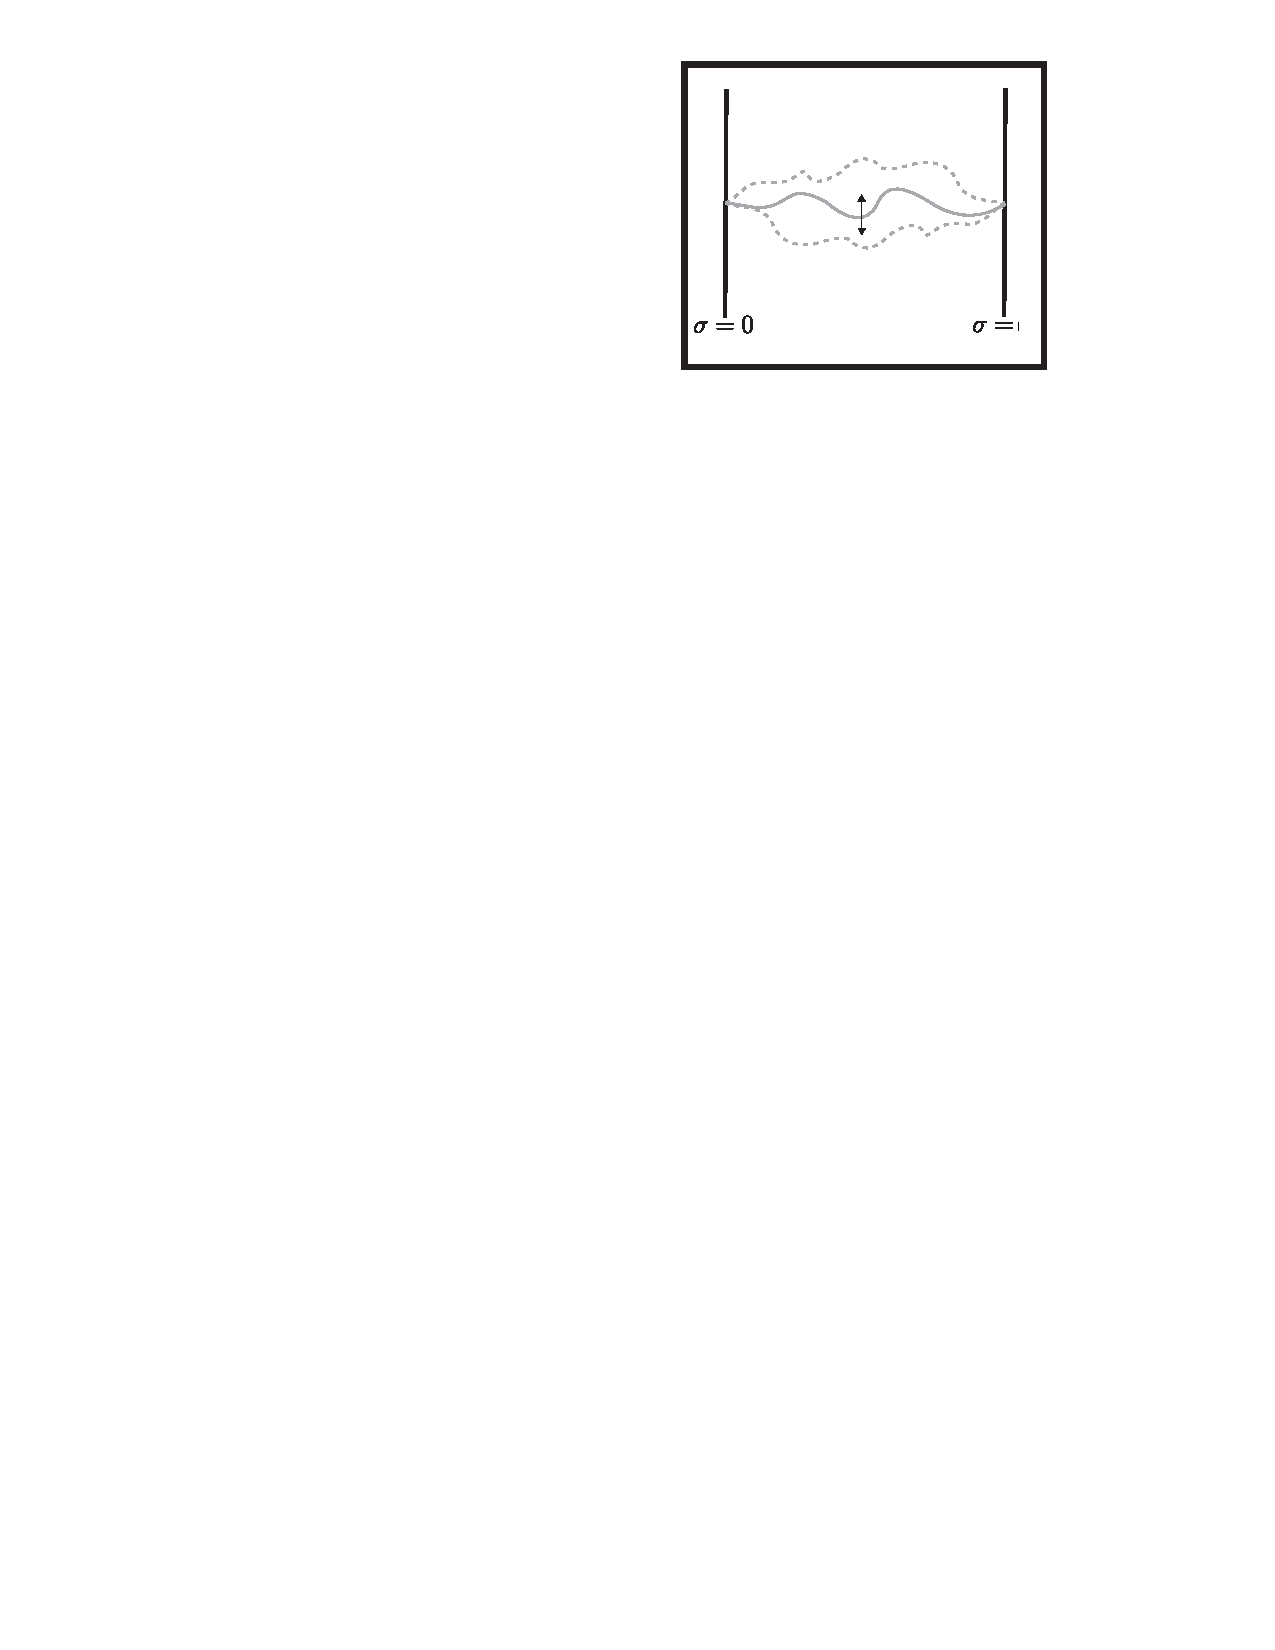
\includegraphics[width=\linewidth]{figure/string-BD}
		\caption{Dirichlet BC’s: The string can oscillate, but its endpoints are fixed at the boundary. The $y$ axis is spacetime direction $X^i$ whereas $x$ axis is worldsheet direction $\sigma$.}
		\label{fig:dirichlet}
	\end{minipage}
	\hfill
	\begin{minipage}[t]{0.48\linewidth}
		\centering
		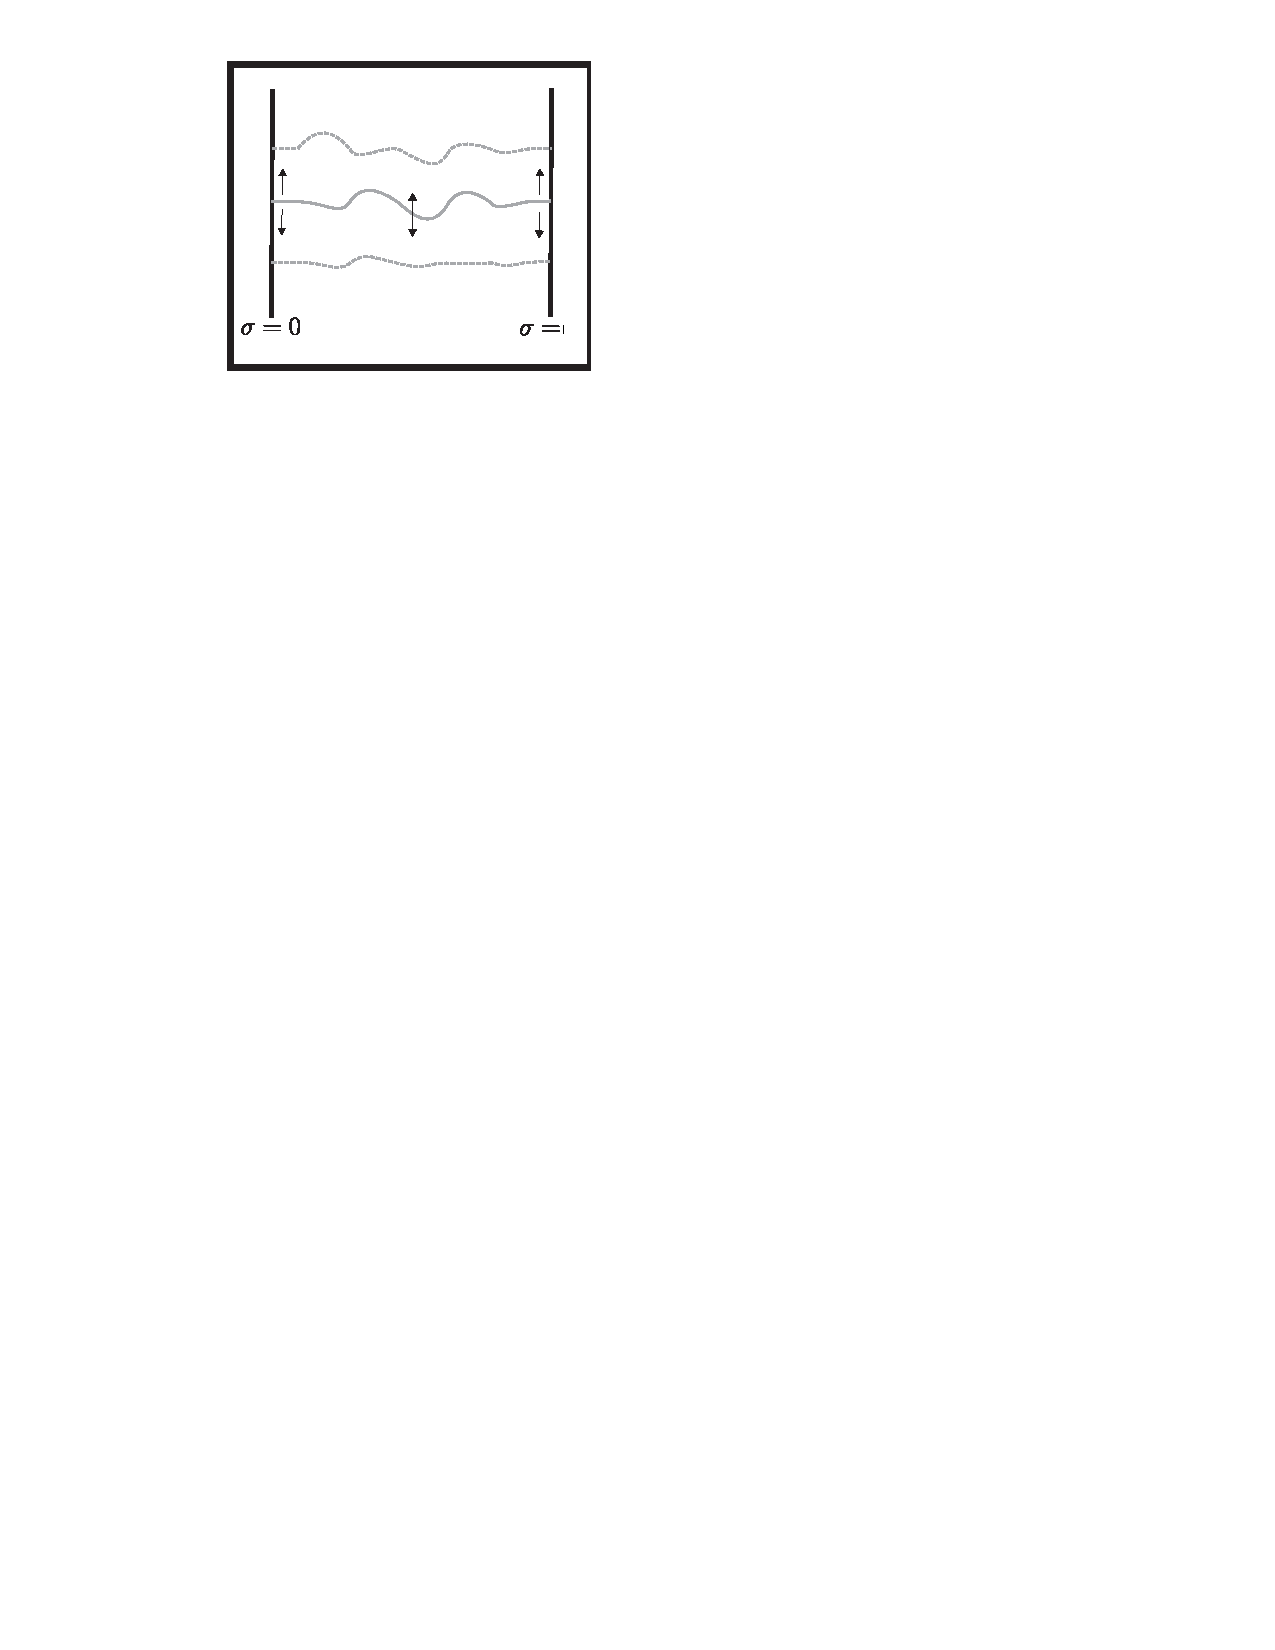
\includegraphics[width=\linewidth]{figure/string-BD1}
		\caption{Neumann BC’s: The string can oscillate and its endpoints can move along the boundaries, as long as their derivatives vanish at the boundaries. }
		\label{fig:neumann}
	\end{minipage}
\end{figure*}
The first two conditions are the only possibilities consistent with $D$-dimensional Poincaré invariance and the equations of motion. The NG and Polyakov actions are perhaps the simplest actions with the given symmetries. But simplicity is not the correct criterion; symmetry is key. 

Now we generalize the Polyakov action, requiring that the symmetries are preserved and that the action is a polynomial in derivatives. 
Global Weyl invariance, i.e., $\omega(\tau, \sigma)=C$ (where $C$ is a constant), requires that $\gamma^{ab}$ appears one more time than $\gamma_{ab}$ to cancel the variation of $(-\gamma)^{1/2}$. Additional upper indices can only contract with derivatives, so each term must have two derivatives. 
Coordinate invariance and Poincaré invariance allow: 
\begin{equation}
	\chi=\frac{1}{4 \pi} \int_{M} \dif \tau \dif \:\sigma(-\gamma)^{1 / 2} R \label{Poincar\'{e}-x}
\end{equation}
where $R$ is the Ricci scalar. 
Under a local Weyl scaling: 
\begin{equation}
	\left(-\gamma^{\prime}\right)^{1 / 2} R^{\prime}=(-\gamma)^{1 / 2}\left(R-2 \nabla^{2} \omega\right)\label{Ricci-Weyl}
\end{equation}
\begin{tcolorbox}[breakable]
	\begin{proof}
		\begin{align*}
			R^\prime &= e^{-2\omega} R - 2 e^{-3\omega} g^{\rho\sigma} \nabla_{\rho} \partial_{\sigma} e^{\omega} + 2 e^{-4\omega} g^{\rho\sigma} (\partial_{\rho} e^{\omega})(\partial_{\sigma} e^{\omega}) \\
			\intertext{Using the chain rule for the scalar $e^{\omega}$, we have $\partial_{\sigma} e^{\omega} = e^{\omega} \partial_{\sigma} \omega$ and $\nabla_{\rho} \partial_{\sigma} e^{\omega} = e^{\omega} (\partial_{\rho} \omega \partial_{\sigma} \omega + \nabla_{\rho} \partial_{\sigma} \omega)$. Substituting these:}
			R^\prime &= e^{-2\omega} R - 2 e^{-3\omega} \left[ e^{\omega} \left( g^{\rho\sigma} \partial_{\rho} \omega \partial_{\sigma} \omega + \square \omega \right) \right] + 2 e^{-4\omega} \left( e^{2\omega} g^{\rho\sigma} \partial_{\rho} \omega \partial_{\sigma} \omega \right) \\
			&= e^{-2\omega} R - 2 e^{-2\omega} (\partial \omega)^2 - 2 e^{-2\omega} \square \omega + 2 e^{-2\omega} (\partial \omega)^2 \\
			&= e^{-2\omega} (R - 2 \square \omega)
		\end{align*}
	\end{proof}
\end{tcolorbox} 
\noindent In (\ref{Ricci-Weyl}), the variation is a total derivative because for any $v^a$, we have $(-\gamma)^{1/2}\nabla_a v^a=\partial_a[(-\gamma)^{1/2}v^a]$. Thus (\ref{Poincar\'{e}-x}) is invariant for a worldsheet without boundaries. With boundaries, there is an extra surface term. 

We can include $\chi$ in the action: 
\begin{equation}
	\begin{aligned}
		S_{\mathrm{P}}^{\prime} &=S_{\mathrm{P}}-\lambda \chi \\
		&=-\int_{M} \dif \tau \dif \sigma\:(-\gamma)^{1 / 2}\left(\frac{1}{4 \pi \alpha^{\prime}} \gamma^{a b} \partial_{a} X^{\mu} \partial_{b} X_{\mu}+\frac{\lambda}{4 \pi} R\right)
	\end{aligned}
\end{equation}
This is the most general (diff $\times$ Weyl)-invariant and Poincaré-invariant action. 
$S_{\mathrm{P}}^\prime$ looks like the Hilbert action $\int (-\gamma)^{1/2}R$ for the (gravitational) metric minimally coupled to $D$ massless scalar fields. However, in 2D, the Hilbert action depends only on the topology of the worldsheet; its variation is $R_{ab}-\frac{1}{2}\gamma_{ab}R$. In 2D, the symmetries of the curvature tensor imply $R_{ab}=\frac{1}{2}\gamma_{ab}R$. The Hilbert action is invariant under continuous transformations of the metric, but has global effects. 
\begin{tcolorbox}
	\begin{remark}
		In 2D, we have $R_{abcd}= \frac{R}{2}\left(\gamma_{ac}\gamma_{bd} - \gamma_{ad}\gamma_{bc}\right)$ and as a result:
		\begin{align}
			R_{ab} &= \gamma^{cd} R_{acbd}= \frac{R}{2}\,\gamma^{cd}\left(\gamma_{ac}\gamma_{bd} - \gamma_{ad}\gamma_{bc}\right)= \frac{R}{2}\left(\delta^d_a \gamma_{bd} - \delta^c_a \gamma_{bc}\right) \nonumber\\[6pt]
			&= \frac{R}{2}\,\gamma_{ab}.
		\end{align} 
	\end{remark}
\end{tcolorbox}

\section{\texorpdfstring{The open string spectrum}{The open string spectrum}}  \label{sec:1.3}
Introduce light-cone coordinates in spacetime: 
\begin{equation}
	x^{\pm}=2^{-1 / 2}\left(x^{0} \pm x^{1}\right), \quad x^{i},\quad  i=2, \ldots, D-1
\end{equation}
Spacetime coordinates are written as $X^\mu$, and fields on the worldsheet are written as $X^\mu(\tau, \sigma)$. 
In these coordinates, the metric is: 
\begin{subequations} \label{1.3.2} %
	\begin{align}
		&a^{\mu} b_{\mu}=-a^{+} b^{-}-a^{-} b^{+}+a^{i} b^{i} \\
		&a_{-}=-a^{+}, \quad a_{+}=-a^{-}, \quad a_{i}=a^{i}
	\end{align} 
\end{subequations}
Let the worldsheet parameter $\tau$ be the spacetime coordinate $X^+$. Then $X^+$ plays the role of time, and $p^-$ is the energy. The longitudinal components $X^-, p^+$ act like spatial coordinates and momentum, as do the transverse $X^i, p^i$. 
Starting from the point particle, using $S_{\mathrm{pp}}^\prime$: 
Fix the worldline parameterization via: 
\begin{equation}
	X^+(\tau)=\tau
\end{equation}
The action becomes: 
\begin{equation}
	S_{\mathrm{pp}}^{\prime}=\frac{1}{2} \int \dif\tau\left(-2 \eta^{-1} \dot{X}^{-}+\eta^{-1} \dot{X}^{i} \dot{X}^{i}-\eta m^{2}\right)
\end{equation}
\begin{tcolorbox}
	\begin{remark}
		Here we used $\dot{X}^{\mu} \dot{X}_{\mu}=-\dot{X}^{+} \dot{X}^{-}-\dot{X}^{+} \dot{X}^{-}+\dot{X}^{i} \dot{X}^{i}=-2 \dot{X}^{-}+\dot{X}^{i} \dot{X}^{i}$. 
	\end{remark}
\end{tcolorbox}
\noindent The canonical momentum $p_{\mu}=\partial L / \partial \dot{X}^{\mu}$ is: 
\begin{equation}
	p_{-}=-\eta^{-1}, \quad p_{i}=\eta^{-1} \dot{X}^{i}
\end{equation}
Using the metric $p^i=p_i$ and $p^+=-p_-$, the Hamiltonian is: 
\begin{equation}
	\begin{aligned}
		H &=p_{-} \dot{X}^{-}+p_{i} \dot{X}^{i}-L \\
		&=-\eta^{-1}\dot{X}^s +\eta p_i p^i +\eta^{-1}\dot{X}^s -\tfrac{1}{2}\eta p_i p_i +\tfrac{1}{2}\eta m^2 \\
		&=\frac{p^{i} p^{i}+m^{2}}{2 \eta^{-1}}=\frac{p^{i} p^{i}+m^{2}}{2 p^{+}}\label{string-H}
	\end{aligned}
\end{equation}
There is no $p_+ X^+$ term because $X^+$ is not a dynamical variable. 
Furthermore, $\dot{\eta}$ does not appear in the action, so $p_\eta=0$. Since $\eta=-1/p_{-}$, we should not treat $\eta$ as an independent canonical coordinate. 

For quantization, impose canonical commutators on the dynamical fields: 
\begin{equation}
	\left[p_{i}, X^{j}\right]=-\mi \delta_{i}^{j}, \quad\left[p_{-}, X^{-}\right]=-\mi
\end{equation}
The momentum eigenstates $|k_-, k^i\rangle$ form a complete set. The remaining momentum components are determined by other quantities. The gauge choice associates $\tau$ with $X^+$, so $H=-p_+ =p^-$. The negative sign between $H$ and $p_+$ is because the former is active and the latter is passive. Thus, (\ref{string-H}) becomes the relativistic mass-shell condition. We have obtained the spectrum of a relativistic scalar. 

Turning to the open string. The coordinate region is $-\infty<\tau<+\infty$ and $0\leq \sigma\leq l$. Choose the following gauge fixing condition to remove Polyakov redundancies. Let: 
\begin{subequations} 
	\begin{align} 
		X^+&=\tau \label{1.3.8a} \\
		\partial_{\sigma} \gamma_{\sigma \sigma}&=0 \label{1.3.8b} \\
		\operatorname{det} \gamma_{a b}&=-1 \label{1.3.8c}
	\end{align}   \label{1.3.8}
\end{subequations}
How to obtain this gauge? 
First, choose $\tau$ according to (\ref{1.3.8a}). Note that $f=\gamma_{\sigma \sigma}\left(-\operatorname{det} \gamma_{a b}\right)^{-1 / 2}$ transforms as: 
\begin{equation}
	f^{\prime} \dif \sigma^{\prime}=f \dif \sigma\label{1.3.9}
\end{equation}
\begin{tcolorbox}[breakable]
	\begin{proof}
		Under a coordinate transformation $x^a \to x'^a$, the metric transforms as
		\begin{equation}
			\gamma_{ab}
			= \frac{\partial x'^c}{\partial x^a}
			\frac{\partial x'^d}{\partial x^b}
			\gamma'_{cd} \, .
		\end{equation}
		with $x^a=(\sigma,\tau)$. In matrix form this may be written as
		\begin{equation}
			\gamma = J^{\mathrm T} \, \gamma' \, J \, ,
		\end{equation}
		where $J^c{}_a = \partial x'^c / \partial x^a$ is the Jacobian matrix. Taking determinants, and using $\det(J^{\mathrm T}) = \det(J)$, we obtain
		\begin{equation}
			\det \gamma 
			= \det(J^{\mathrm T}) \, \det(\gamma') \, \det(J)
			= (\det J)^2 \det \gamma' \, .
		\end{equation}
		
		For the specific transformation $\tau' = \tau$, $\sigma' = \sigma'(\sigma,\tau)$, the Jacobian takes the triangular form
		\begin{equation}
			J =
			\begin{pmatrix}
				\displaystyle \frac{\partial \sigma'}{\partial \sigma} & \displaystyle \frac{\partial \sigma'}{\partial \tau} \\
				0 & 1
			\end{pmatrix} \, ,
		\end{equation}
		so that
		\begin{equation}
			\det J = \frac{\partial \sigma'}{\partial \sigma} \, .
		\end{equation}
		Hence,
		\begin{equation}
			\det \gamma
			= \left(\frac{\partial \sigma'}{\partial \sigma}\right)^2 \det \gamma' \, .
		\end{equation}
		One can prove \eqref{1.3.9} together with the following
		\begin{align}
			\gamma_{\sigma'\sigma'}&=\pdv{\sigma}{\sigma'}\pdv{\sigma}{\sigma'}\gamma_{\sigma\sigma}\\
			\dif \sigma'&=\pdv{\sigma'}{\sigma}\dif \sigma
		\end{align}
	\end{proof}
\end{tcolorbox}
Define the invariant length $\dif l=f\dif \sigma$. Define the $\sigma$ coordinate of a point proportional to the invariant length from $\sigma=0$ to that point. The proportionality constant is determined by keeping the right endpoint at $\sigma=l$. In this coordinate system, $f=\dif l/\dif \sigma$ is independent of $\sigma$, though it may depend on $\tau$. 
Finally, perform a Weyl transformation to satisfy (\ref{1.3.8c}). Since $f$ is Weyl-invariant, $\partial_\sigma f$ remains zero. Combined with (\ref{1.3.8c}), this implies $\partial_{\sigma} \gamma_{\sigma \sigma}=0$, so (\ref{1.3.8b}) is also satisfied. 

For $\gamma_{\tau\tau}(\tau, \sigma)$, we can solve the gauge condition (\ref{1.3.8c}). Since $\gamma_{\sigma\sigma}$ is independent of $\sigma$, the only independent degrees of freedom in the metric are now $\gamma_{\sigma\sigma}(\tau)$ and $\gamma_{\sigma\tau}(\tau, \sigma)$. 
The inverse metric is: 
\begin{equation}
	\begin{bmatrix}
		\gamma^{\tau \tau} & \gamma^{\tau \sigma} \\
		\gamma^{\sigma \tau} & \gamma^{\sigma \sigma}
	\end{bmatrix}=
	\begin{bmatrix}
		-\gamma_{\sigma \sigma}(\tau) & \gamma_{\tau \sigma}(\tau, \sigma) \\
		\gamma_{\tau \sigma}(\tau, \sigma) & \gamma_{\sigma \sigma}^{-1}(\tau)\left(1-\gamma_{\tau \sigma}^{2}(\tau, \sigma)\right)
	\end{bmatrix}
\end{equation}
\begin{tcolorbox}[breakable]
	\begin{proof}
		\[
		\begin{bmatrix}
			\gamma_{\tau \tau} & \gamma_{\tau \sigma} \\
			\gamma_{\tau \sigma} & \gamma_{\sigma\sigma}
		\end{bmatrix}
		\begin{bmatrix}
			\gamma^{\tau\tau} & \gamma^{\tau \sigma} \\
			\gamma^{\tau \sigma} & \gamma^{\sigma \sigma}
		\end{bmatrix}
		=\begin{bmatrix}
			-\gamma_{\tau \tau} \gamma_{\sigma \sigma}+\gamma_{\tau \sigma}^{2} &  \gamma_{\tau\tau} \gamma_{\tau \sigma}+\gamma_{\tau \sigma} \gamma_{\sigma \sigma}^{-1}\left(1-\gamma_{\tau \sigma}^{2}\right) \\
			-\gamma_{\sigma \sigma} \gamma_{\tau \sigma}+\gamma_{\sigma \sigma} \gamma_{\tau \sigma} & \gamma_{\tau \sigma}^{2}+1-\gamma_{\tau \sigma}^{2}  
		\end{bmatrix}
		\]
		Then use (\ref{1.3.8c}) given by $\gamma_{\tau\tau} \gamma_{\sigma \sigma}-\gamma_{\tau \sigma}^{2}=-1$. 
	\end{proof} 
\end{tcolorbox}
\noindent Thus, the Polyakov Lagrangian becomes: 
\begin{equation}
	\begin{aligned}
		L&=-\frac{1}{4 \pi \alpha^{\prime}} \int_{0}^{\ell} \dif\sigma\: \Bigl[\gamma_{\sigma \sigma}\left(2 \partial_{\tau} x^{-}-\partial_{\tau} X^{i} \partial_{\tau} X^{i}\right) \\
		&\qquad \quad-2 \gamma_{\sigma \tau}(\partial_{\sigma} Y^{-}-\partial_{\tau} X^{i} \partial_{\sigma} X^{i})
		+\gamma_{\sigma \sigma}^{-1}(1-\gamma_{\tau \sigma}^{2}) \partial_{\sigma} X^{i} \partial_{\sigma} X^{i}\Bigr]
	\end{aligned}
\end{equation}
\begin{tcolorbox}[breakable]
	\begin{proof}
		Expand the Polyakov action (\ref{1.2.13}) by components:
		\begin{align*}
			L=-\frac{1}{4 \pi \alpha^{\prime}} \int_{0}^{\ell} \dif\sigma \:\Bigl[-\gamma_{\sigma \sigma}\underbrace{(\partial_\tau X^{\mu} \partial_\tau X_{\mu})}_{(1)} 
			+2 \gamma_{\tau \sigma}\underbrace{(\partial_{\tau} X^{\mu} \partial_{\sigma} X_{\mu})}_{(2)} 
			+\gamma_{\sigma \sigma}^{-1}(1-\gamma_{\tau \sigma}^{2}) \underbrace{(\partial_{\sigma} X^{\mu} \partial_{\sigma} X_{\mu})}_{(3)}\Bigr] 
		\end{align*}
		where
		\begin{align*}
			(1) &=-\dot{X}^{+} \dot{X}^{-}-\dot{X}^{+} \dot{X}^{-}+\dot{X}^{i} \dot{X}^{i} =-2 \partial_{\tau} X^{-}+\partial_{\tau} X^{i} \partial_{\tau} X^{i} \\
			(2) &=-\partial_{\tau} X^{\dagger} \partial_{\sigma} X^{-}-\partial_{\tau} X^{-} \partial_{\sigma} X^{+}+\partial_{\tau} X^{i} \partial_{\sigma} X^{i} \\
			&=-\partial_{\sigma} X^{-}-\partial_{\tau} X^{-} \partial_{\sigma} \tau+\partial_{\tau} X^{i} \partial_{\tau} X^{i} =-\left(\partial_{\sigma} Y^{-}-\partial_{\tau} X^{i} \partial_{\sigma} X^{i}\right) \\
			(3) &=-\partial_{\sigma} X^{-} \partial_{\sigma} X^{+}-\partial_{\sigma} X^{+} \partial_{\sigma} X^{-}+\partial_{\sigma} X^{i} \partial_{\sigma}X^{i} 
			=\partial_{\sigma} X^{i} \partial_{\sigma} X^{i}
		\end{align*}
		Q.E.D. 
	\end{proof}
\end{tcolorbox}
\noindent Here we split $X^-(\tau, \sigma)$ into two parts: $x^-(\tau)$ and $Y^-(\tau, \sigma)$. $x^-(\tau)$ is the average value of $X^-$ at time $\tau$. 
\begin{subequations}
	\begin{align}
		x^{-}(\tau)&=\frac{1}{\ell} \int_{0}^{\ell} \dif \sigma X^{-}(\tau, \sigma) \\
		Y^{-}(\tau, \sigma)&=X^{-}(\tau, \sigma)-x^{-}(\tau)
	\end{align}
\end{subequations}
$Y^-$ does not appear in terms containing time derivatives and is thus non-dynamical. It acts like a Lagrange multiplier, constraining $\partial_\sigma \gamma_{\tau\sigma}$ to be zero. 
Under gauge (\ref{1.3.8}), the open string boundary condition (\ref{Neumann-bound}) becomes: 
\begin{equation}
	\gamma_{\tau \sigma} \partial_{\tau} X^{\mu}-\gamma_{\tau \tau} \partial_{\sigma} X^{\mu}=0 \quad \text { at } \sigma=0, \ell
\end{equation}
\begin{proof}
	$
	\partial^{\sigma} X^{\mu} =\gamma^{\sigma a} \partial_{a} X^{\mu}=\gamma^{\sigma \tau} \partial_{\tau} X^{\mu}+\gamma^{\sigma \sigma} \partial_{\sigma} X^{\mu} =\gamma_{\tau \sigma} \partial_{\tau} X^{\mu}+\gamma_{\sigma \sigma}^{-1}\left(1-\gamma_{\tau \sigma}^{2}\right) \partial_{\sigma} X^{\mu} =\gamma_{\tau \sigma} \partial_{\tau} X^{\mu}-\gamma_{\tau \tau} \partial_{\sigma} X^{\mu}
	$
	Q.E.D. 
\end{proof}
\noindent For $\mu=+$: 
\begin{equation}
	\gamma_{\tau \sigma}=0 \quad \text { at } \sigma=0, \ell
\end{equation}
Since $\partial_\sigma \gamma_{\tau\sigma}=0$, $\gamma_{\tau\sigma}$ vanishes everywhere. 
For $\mu=i$, the boundary condition is: 
\begin{equation}
	\partial_{\sigma} X^{i}=0 \quad \text { at } \sigma=0, \ell   \label{bound-mu-i}
\end{equation}
Imposing gauge conditions and including the Lagrange multiplier $Y^-$, the Lagrangian is: 
\begin{equation}
	L=-\frac{\ell}{2 \pi \alpha^{\prime}} \gamma_{\sigma \sigma} \partial_{\tau} x^{-}+\frac{1}{4 \pi \alpha^{\prime}} \int_{0}^{\ell} \dif\sigma\,\Bigl(\gamma_{\sigma \sigma} \partial_{\tau} X^{i} \partial_{\tau} X^{i}-\gamma_{\sigma \sigma}^{-1} \partial_{\sigma} X^{i} \partial_{\sigma} X^{i}\Bigr)
\end{equation}
The conjugate momentum to $x^-$ is: 
\begin{equation}
	p_{-}=-p^{+}=\frac{\partial L}{\partial\left(\partial_{\tau} x^{-}\right)}=-\frac{\ell}{2 \pi \alpha^{\prime}} \gamma_{\sigma \sigma}\label{1.3.17}
\end{equation}
As with the einbein $\eta$ in the particle case, $\gamma_{\sigma\sigma}$ is momentum rather than a coordinate. 
The conjugate momentum density to $X^i(\tau, \sigma)$ is: 
\begin{equation}
	\Pi^{i}=\frac{\delta L}{\delta\left(\partial_{\tau} X^{i}\right)}=\frac{1}{2 \pi \alpha'} \gamma_{\sigma \sigma} \partial_{\tau} X^{i}=\frac{p^{+}}{\ell} \partial_{\tau} X^{i} \label{1.3.18}
\end{equation}
Thus, the Hamiltonian is: 
\begin{align}
	H &=p_{-} \partial_{\tau} x^{-}-L+\int_{0}^{\ell} \dif \sigma\: \Pi_{i} \partial_{\tau} X^{i} \nonumber \\
	&= p_{-} \partial_{\tau}  x^{-}-p_{-} \partial_{\tau} x^{-} -\frac{1}{4 \pi \alpha^{\prime}} \int_{0}^{\ell} \dif \sigma\:\biggl(\gamma_{\sigma \sigma} \partial_{\tau} X^{i} \partial_{\tau} X^{i}-\frac{\partial_{\sigma} X^{i} \partial_{\sigma} X^{i}}{\gamma_{\sigma \sigma}}\biggr) 
	+\int_{0}^{\ell} \dif \sigma\: \frac{\ell\,\Pi_{i}^{2} }{ p^{+}} \nonumber \\
	&=\frac{\ell}{4 \pi \alpha^{\prime} p^{+}} \int_{0}^{\ell} \dif \sigma\, 4 \pi \alpha^{\prime}\Pi_{i}^{2} -\frac{\gamma_{\sigma\sigma}^{-1}}{4 \pi \alpha^{\prime}} \int_{0}^{\ell} \dif \sigma\,\Bigl(\left(2 \pi \alpha^{\prime} \Pi^{i}\right)^{2}-\partial_\sigma X^{i} \partial _\sigma X^{i} \Bigr)\nonumber \\
	&=\frac{\ell}{4 \pi \alpha^{\prime} p^{+}} \int_{0}^{\ell} d \sigma\left(2 \pi \alpha^{\prime} \Pi^{i} \Pi^{i}+\frac{1}{2 \pi \alpha^{\prime}} \partial_{\sigma} X^{i} \partial_{\sigma} X^{i}\right) \label{1.3.19}
\end{align}
This is precisely the Hamiltonian for $D-2$ free fields $X^i$, where $p^+$ is a conserved quantity. 
The equations of motion are: 
\begin{subequations}
	\begin{align}
		\partial_{\tau} x^{-}&=\frac{\partial H}{\partial p_-}=-\frac{\partial H}{\partial p^{+}}=-\frac{H p^{+} \partial(p^+)^{-1}}{\partial p^{+}}=\frac{H}{p^+} \:,\quad
		\partial_{\tau} p^{+}=\frac{\partial H}{\partial x^{-}}=0 \\
		\partial_{\tau} X^{i}&=\frac{\delta H}{\delta \Pi^{i}}=\frac{\ell}{2 p^{+}} 2 \Pi^{i}=2 \pi\alpha^{\prime}c\Pi^{i} \:,\quad
		\partial_\tau \Pi^{i}=-\frac{\delta H}{\delta X^{i}}=\frac{c}{2 \pi \alpha^{\prime}} \partial_{\sigma}^{2} X^{i} \:,
	\end{align}
\end{subequations}
where $c=\ell/(2 \pi \alpha^{\prime} p^{+})$. 
This leads to the wave equation: 
\begin{equation}
	\partial_{\tau}^{2} X^{i}=c^{2} \partial_{\sigma}^{2} X^{i}
\end{equation}
Choose $\ell$ such that $c=1$. Thus $p^+$ is conserved, and the total string length $\ell$ remains constant. 

$X^\pm$ also satisfy the wave equation. $X^-$ requires some calculation. Under (\ref{bound-mu-i}), the general solution to the wave equation is: 
\begin{equation}
	X^{i}(\tau, \sigma)=x^{i}+\frac{p^{i}}{p^{+}} \tau+\mi\left(2 \alpha^{\prime}\right)^{1 / 2} \sum_{n=-\infty \atop n \neq 0}^{\infty} \frac{1}{n} \alpha_{n}^{i} \exp \left(-\frac{\pi \mi n c \tau}{\ell}\right) \cos \frac{\pi n \sigma}{\ell} \label{1.3.22}
\end{equation}
where we write the expansion coefficient $A_n=\sqrt{2\alpha'}\frac{\alpha_n^i}{n}$ to make \eqref{1.3.25b} cleaner and the purpose of $\sqrt{2\alpha'}$ factor is to make the constants $\alpha_n^i$ dimensionless. The reality of $X^i$ requires $\alpha_{-n}^{i}=\left(\alpha_{n}^{i}\right)^{\dagger}$. 
Define center-of-mass variables: 
\begin{subequations}
	\begin{align}
		x^{i}(\tau)&=\frac{1}{\ell} \int_{0}^{\ell} \dif \sigma\: X^{i}(\tau, \sigma) \\
		p^{i}(\tau)&=\int_{0}^{\ell} \dif \sigma\: \Pi^{i}(\tau, \sigma)=\frac{p^{+}}{\ell} \int_{0}^{\ell} \dif \sigma \:\partial_{\tau} X^{i}(\tau, \sigma)
	\end{align}
\end{subequations}
These represent the average mass and total momentum. These are Heisenberg operators. 
In (\ref{1.3.22}), they are Schrödinger operators $x^{i} \equiv x^{i}(0)$ and $p^{i} \equiv p^{i}(0)$. 
For quantization, impose commutation relations: 
\begin{subequations}
	\begin{align}
		\left[x^{-}, p^{+}\right]&=\mi \eta^{-+}=-\mi  \label{1.3.24a}\\
		\left[X^{i}(\sigma), \Pi^{j}\left(\sigma^{\prime}\right)\right]&=\mi \delta^{i j} \delta\left(\sigma-\sigma^{\prime}\right)
		\label{1.3.24b}
	\end{align}
\end{subequations}
Written in terms of Fourier components: 
\begin{subequations}
	\begin{align}
		\left[x^{i}, p^{j}\right]&=\mi \delta^{i j}   \label{1.3.25a}\\
		\left[\alpha_{m}^{i}, \alpha_{n}^{j}\right]&=m \delta^{i j} \delta_{m,-n}   \label{1.3.25b}
	\end{align} \label{1.3.25}
\end{subequations}
\noindent For each $m$ and $i$, the modes satisfy the harmonic oscillator algebra: 
\begin{equation}
	\alpha_{m}^{i} \sim m^{1 / 2} a, \quad \alpha_{-m}^{i} \sim m^{1 / 2} a^{\dagger}, \quad m>0
\end{equation}
where $[a, a^\dagger]=1$. 
\begin{tcolorbox}[breakable]
	\begin{proof}
		Equations (\ref{1.3.24b}), (\ref{1.3.25a}), and (\ref{1.3.25b}) form a logical loop; knowing any two allows derivation of the third. 
		Assume the latter two are known to prove the first. Introduce the notation:
		\[\sideset{}{'}\sum={\sum_{n=-\infty\atop n \neq 0}^{+\infty} }\]
		From (\ref{1.3.18}) and (\ref{1.3.22}), we have:
		\begin{align}
			\Pi^{i}(\tau, \sigma)
			=&\frac{p^{i}}{\ell}+\frac{p^+}{\ell}\mi \left(2 \alpha^{\prime}\right)^{1 / 2} \sideset{}{'}\sum \frac{1}{n} \alpha_{n}^{i}\left(-\frac{\pi \mi n c}{\ell}\right) \exp \left(-\frac{\pi \mi n c \tau}{\ell}\right) \cos \frac{n \pi \sigma}{\ell} \nonumber \\
			=&\frac{p^ i}{\ell}+\frac{1}{\left(2 \alpha^{\prime}\right)^{1 / 2} \ell} \sideset{}{'}\sum \alpha_{n}^{i} \exp \left(-\frac{\pi \mi n c\tau}{\ell}\right) \cos \frac{n \pi \sigma}{\ell} \tag{1.a} \label{1.a}
		\end{align}
		where we used:
		\[
		\mi\left(2 \alpha^{\prime }\right)^{1 / 2} \frac{-\mi \pi c}{\ell}=\pi\left(2 \alpha^{\prime}\right)^{1 / 2} \frac{1}{2 \alpha^{\prime} \pi p^{+}}=\frac{1}{(2 \alpha^\prime)^{1 / 2} p^{+}}
		\]
		Then:
		\[
		[X^{i} , \Pi^{i}]=\frac{1}{\ell}\left[x^{i} , p^{i}\right]+\frac{\mi}{\ell } \sideset{}{'}\sum_{n,m} \frac{1}{n} \exp \left(-\frac{\pi \mi n c \tau}{\ell}\right) \cos \frac{n \pi \sigma}{\ell}
		\left[\alpha_{n}^{i}, \alpha_{m}^{i}\right] \exp \left(-\frac{\pi \mi m c \tau}{\ell}\right) \cos \frac{m \pi \sigma^\prime}{\ell}
		\]
		Let $\left[\alpha_{m}^{i}, \alpha_{n}^{i}\right]=m \delta_{m,-n}$. Given the completeness relation:
		\[
		2\pi\delta(\sigma^{\prime}-\sigma)=\sum_{n=-\infty}^{+\infty} \me^{ \mi n\left(\sigma^{\prime}-\sigma\right)}
		=1+\sideset{}{'}\sum \me^{  \mi n \left(\sigma^{\prime}-\sigma\right)}
		\]
		The latter term becomes:
		\begin{align*}
			&\quad -\frac{\mi}{\ell} {\sum}^\prime \frac{1}{n} \exp \left(-\frac{\pi \mi n c \tau}{\ell}\right) \cos \frac{n \pi \sigma}{\ell}(-n)  \exp \left(+\frac{\pi \mi n c \tau}{\ell}\right) \cos \frac{-n \pi \sigma^\prime}{\ell}\\
			&=\frac{\mi}{\ell} {\sum}^\prime \cos\frac{n \pi \sigma}{\ell} \cos \frac{n \pi \sigma^{\prime}}{\ell} \\
			&=\frac{\mi}{ 4\ell}  {\sum}^\prime \Bigl[\me^{\mi n \pi(\sigma+\sigma^{\prime})/\ell}+\me^{-\mi n \pi(\sigma+\sigma^{\prime})/\ell}+ \me^{\mi n \pi(\sigma-\sigma^{\prime})/\ell}+\me^{-\mi n \pi(\sigma-\sigma^{\prime})/\ell}\Bigr]\\
			&=\frac{\mi}{2\ell} \Bigl( 2\pi\delta\bigl(\pi(\sigma+\sigma^{\prime})/\ell\bigr)-1+2\pi\delta\bigl(\pi(\sigma-\sigma^{\prime})/\ell\bigr)-1 \Bigr) \\
			&=-\frac{\mi}{\ell}+\frac{\mi \pi}{ \ell} \delta\bigl(\pi(\sigma-\sigma^{\prime})/\ell\bigr) 
			=-\frac{\mi}{\ell}+\mi \delta(\sigma-\sigma^{\prime})
		\end{align*}
		Note $\delta(\sigma-\sigma^\prime)=\delta(\sigma^\prime-\sigma)$, giving a factor of 2; and $\sigma, \sigma^\prime>0$ makes $\delta\bigl(\pi(\sigma+\sigma^{\prime})/\ell\bigr)=0$. 
		Since $[x^{i}, p^{i}]=\mi$, we have:
		$$\left[X^{i} , \Pi^{i}\right]=\mi \delta(\sigma-\sigma^{\prime})$$ 
		Q.E.D.
	\end{proof}
\end{tcolorbox}
The state $|0;k \rangle$ (where $k=(k^+, k^i)$) is annihilated by lowering operators and is an eigenstate of the center-of-mass momentum: 
\begin{subequations}
	\begin{align}
		p^{+}|0 ; k\rangle&=k^{+}|0 ; k\rangle, \quad p^{i}|0 ; k\rangle=k^{i}|0 ; k\rangle \\
		\alpha_{m}^{i}|0 ; k\rangle&=0, \quad m>0
	\end{align}
\end{subequations}
General states are obtained by acting with raising operators on $|0;k \rangle$: 
\begin{equation}
	|N ;  k\rangle=\left[\prod_{i=2}^{D-1} \prod_{n=1}^{\infty} \frac{\left(\alpha_{-n}^{i}\right)^{N_{i n}}}{\left(n^{N_{i n}} N_{i n} !\right)^{1 / 2}}\right]|0 ; k\rangle\label{general-state}
\end{equation}
Independent states can be labeled by center-of-mass momenta $k^+, k^i$ and occupation numbers $N_{in}$. Center-of-mass momentum represents the point particle degrees of freedom, while oscillators represent infinite internal degrees of freedom. From a spacetime view, each choice of occupation numbers corresponds to a different particle state or spin. States (\ref{general-state}) form the single open string Hilbert space $\mathscr{H}$. 
In particular, state $|0;0 \rangle$ is the ground state of a single string with zero momentum, not the vacuum state without strings. We call the latter $|\text{vacuum} \rangle$. Operators acting on it cannot create or annihilate strings, but only act on the state space of individual strings. The $n$-string Hilbert space $\mathscr{H}_n$ is formed by the product of $n$ spaces of (\ref{general-state}); wave functions must be symmetric, as all these states have integer spin (to be proven). 
In the free limit, the total Hilbert space of string theory is: 
\begin{equation}
	\mathscr{H}=\lvert \text{vacuum}\rangle \oplus \mathscr{H}_{1} \oplus \mathscr{H}_{2} \oplus \ldots
\end{equation}
Substituting (\ref{1.3.22}) into (\ref{1.3.19}) yields: 
\begin{equation}
	H=\frac{p^{i} p^{i}}{2 p^{+}}+\frac{1}{2 p^{+} \alpha^{\prime}}\left(\sum_{n=1}^{\infty} \alpha_{-n}^{i} \alpha_{n}^{i}+A\right)
\end{equation}
\begin{tcolorbox}[breakable]
	\begin{proof}
		First, split the string Hamiltonian (\ref{1.3.19}) into two parts:
		\begin{align*}
			H_{\Pi}=\frac{\ell}{2 p^+} \int_{0}^{\ell} \dif \sigma \: \Pi^{i} \Pi^{i}\:, \quad 
			H_{X}=\frac{\ell}{2p^{+}(2 \pi \alpha^\prime)^{2} } \int_{0}^{\ell} \dif \sigma \:\partial_{\sigma} X^{i} \partial_{\sigma} X^{i} \:. 
		\end{align*}  
		Using (\ref{1.a}), we have:
		\begin{align*}
			H_\Pi&=\frac{\ell}{2 p^+} \int_{0}^{\ell} \dif \sigma \:
			\Biggl( \frac{p^{i} p^{i}}{\ell^{2}}
			+\frac{1}{2 \alpha^\prime \ell^2} \sideset{}{'}\sum_{n,m} \alpha_{n}^{i} \alpha_{m}^{i}\exp\Bigl(-\frac{\pi \mi c \tau}{\ell}(n+m)\Bigr)  \cos \frac{n \pi \sigma}{\ell} \cos \frac{m\pi \sigma}{\ell}  \\
			&\qquad \qquad\qquad  +\frac{2p^{i}}{\left(2 \alpha^{\prime}\right)^{1 / 2 } \ell^{2}} \sideset{}{'}\sum \alpha_{n}^{i} \exp \left(-\frac{\pi \mi n c \tau}{\ell}\right) \cos \frac{n \pi \sigma}{\ell} \Biggr) \\
			&=\frac{p^{i}p^{i}}{2p^{+}}+\frac{1}{4p^{+}\alpha'}\sideset{}{'}\sum_{n,m} \alpha_{n}^{i} \alpha_{m}^{i}\exp\Bigl(-\frac{\pi \mi c \tau}{\ell}(n+m)\Bigr)\bigl(\delta_{n,m}+\delta_{n,-m}\bigr)/2
		\end{align*}
		Using (\ref{1.3.22}), we have:
		\begin{align*}
			\partial_\sigma X^{i} =-\frac{\mi\left(2 \alpha^{\prime}\right)^{1 / 2} \pi}{\ell} \sideset{}{'}\sum \alpha_{n}^{i} \exp \Bigl(-\frac{\pi \mi n c \tau}{\ell}\Bigr) \sin \frac{n \pi \sigma}{\ell} \:,
		\end{align*}
		Then:
		\begin{align*}
			H_X &=\frac{\ell}{2p^{+}(2 \pi \alpha^\prime)^{2} } \frac{-2 \alpha^\prime \pi^2}{\ell^2} \int_{0}^{\ell} \dif \sigma \sideset{}{'}\sum _{n,m} \alpha_{n}^{i}\alpha_{m}^{i} 
			\exp \Bigl(-\frac{\pi \mi c \tau}{\ell}(n+m)\Bigr) \sin \frac{n \pi \sigma}{l}\sin \frac{m \pi \sigma}{\ell} \\
			&=-\frac{1}{4p^{+}\alpha^\prime  }  \sideset{}{'}\sum _{n,m} \alpha_{n}^{i}\alpha_{m}^{i} 
			\exp \Bigl(-\frac{\pi \mi c \tau}{\ell}(n+m)\Bigr) \bigl(\delta_{n,m}-\delta_{n,-m}\bigr)/2
		\end{align*}
		So:
		\begin{align*}
			H&=H_{\Pi}+H_{X}=\frac{p^{i}p^{i}}{2p^{+}} +\frac{1}{4p^{+}\alpha'}\sideset{}{'}\sum_{n,m} \alpha_{n}^{i} \alpha_{m}^{i}\exp\Bigl(-\frac{\pi \mi c \tau}{\ell}(n+m)\Bigr)\delta_{n,-m} \\
			&=\frac{p^{i}p^{i}}{2p^{+}} +\frac{1}{4p^{+}\alpha'}\sideset{}{'}\sum_{m} \alpha_{-m}^{i} \alpha_{m}^{i}
		\end{align*}
		And:
		\begin{align*}
			\sum_{n} \alpha_{-n}^{i} \alpha_{n}^{i}&=\sum_{n=-\infty}^{-1} \alpha_{-n}^{i} \alpha_{n}^{i}+\sum_{n=1}^{\infty} \alpha_{-n}^{i} \alpha_{n}^{i}=\sum_{n=\infty}^{1} \alpha_{n}^{i} \alpha_{-n}^{i}+\sum_{n=1}^{\infty} \alpha_{-n}^{i} \alpha_{n}^{i}=\sum_{n=1}^{\infty} (\alpha_{n}^{i} \alpha_{-n}^{i}+\alpha_{-n}^{i} \alpha_{n}^{i})\\
			&=2 \sum_{n=1}^{\infty} \alpha_{-n}^{i} \alpha_{n}^{i}+\sum_{n=1}^{\infty} n\delta^{ii}=2 \sum_{n=1}^{\infty} \alpha_{-n}^{i} \alpha_{n}^{i}+(D-2)\sum_{n=1}^{\infty} n
		\end{align*}
		Since $i=2,3...,D-1$, thus $A=(D-2)\sum_{n=1}^{\infty}n/2=(D-2)\zeta(-1)/2$. 
		Q.E.D.
	\end{proof}
\end{tcolorbox}
\noindent In this $H$, the operator ordering is ambiguous. We have placed lowering operators on the right and raising operators on the left. The constant $A$ in Hamiltonian arises from the commutators. In the detailed treatment of light-cone quantization, the constant is determined as follows: the choice of light-cone gauge obstructs the theory's Lorentz invariance. By seeking the generator of Lorentz transformations $M^{\mu\nu}$ and verifying its algebra with $p^\mu$ and other operators, only one case is consistent: $A=-1$. The corresponding spacetime dimension is $D=26$. 

In light-cone quantization, we do not wish to dwell too much on this. We will obtain the values of $A$ and $D$ using conformal gauge methods. It will show us why incorrect values of $A$ and $D$ in the light-cone method lose Lorentz invariance. 
First, we consider the operator ordering constant in the Hamiltonian to originate from the sum of zero-point energies of each oscillator mode. 
For a bosonic field like $X^\mu$, this is $\omega/2$. The expressions $\frac{1}{2} \omega\left(a a^{\dagger}+a^{\dagger} a\right)$ and $\omega\left(a^{\dagger} a+\frac{1}{2}\right)$ are equivalent. In $H$: 
\begin{equation}
	A=\frac{D-2}{2} \sum_{n=1}^{\infty} n \:, \label{1.3.31}
\end{equation}
where $D-2$ comes from the sum over transverse directions. This zero-point energy diverges. Using renormalization techniques: 
\begin{equation}
	\sum_{n=1}^{\infty} n \rightarrow-\frac{1}{12} \:.  \label{1.3.32}
\end{equation}
To obtain this, insert a smooth cutoff factor: 
\begin{equation}
	\exp (-\epsilon \gamma_{\sigma \sigma}^{-1 / 2}|k_{\sigma}|)=	\exp \left(-\frac{n\pi\epsilon}{\sqrt{\gamma_{\sigma\sigma}}\ell}\right) \label{1.3.33}
\end{equation}
where $k_\sigma=n\pi/\ell$. The factor $\gamma_{\sigma\sigma}^{-1/2}$ ensures invariance under $\sigma$ reparameterization $(dl=\int_{0}^{\ell} \sqrt{\gamma_{\sigma\sigma}}d\sigma=\sqrt{\gamma_{\sigma\sigma}}\int_0^{\ell}d\sigma)$. 
\begin{equation}
	\begin{aligned}
		A & \rightarrow \frac{D-2}{2} \sum_{n=1}^{\infty} n \exp \left[-\epsilon n\left(\pi / 2 p^{+} \alpha^{\prime} \ell\right)^{1 / 2}\right]\\
		&=\frac{D-2}{2}\left(\frac{2 \ell p^{+} \alpha^{\prime}}{\epsilon^{2} \pi}-\frac{1}{12}+O(\epsilon)\right)
	\end{aligned}
\end{equation}
The first term of the cutoff is proportional to the string length $\ell$ and can be canceled by counterterms in the action proportional to $\int \dif^2\sigma(-\gamma)^{1/2}$. 
In fact, Weyl invariance $\gamma_{\sigma\sigma}\to e^{2\omega}\gamma_{\sigma\sigma}$ requires it to be canceled, leaving only the cutoff-independent second term: 
\begin{equation}
	A=\frac{2-D}{24}
\end{equation}
\begin{tcolorbox}
	\begin{proof}
		From \eqref{1.3.17} we have $\gamma_{\sigma\sigma}=\frac{2\pi\alpha'p^{+}}{\ell}$ thus \eqref{1.3.31} becomes:
		\begin{equation}
			\begin{aligned}
				A & \rightarrow \frac{D-2}{2} \sum_{n=1}^{\infty} n \exp \left[-\epsilon n\left(\pi / 2 p^{+} \alpha^{\prime} \ell\right)^{1 / 2}\right]\\
				&=-\frac{D-2}{2} \dv{[\epsilon\left(\pi / 2 p^{+} \alpha^{\prime} \ell\right)^{1 / 2}]}\sum_{n=1}^{\infty} \exp \left[-\epsilon n\left(\pi / 2 p^{+} \alpha^{\prime} \ell\right)^{1 / 2}\right]
			\end{aligned}
		\end{equation}
		This is geometric series and the summation is known to be:
		\begin{equation}
			\begin{aligned}
				&=\frac{D-2}{2} \dv{\epsilon\left(\pi / 2 p^{+} \alpha^{\prime} \ell\right)^{1 / 2}}\left[\frac{1}{1-\exp \left[\epsilon\left(\pi / 2 p^{+} \alpha^{\prime} \ell\right)^{1 / 2}\right]}\right]\\
				&=\frac{D-2}{2}\left(\frac{2 \ell p^{+} \alpha^{\prime}}{\epsilon^{2} \pi}-\frac{1}{12}+O(\epsilon)\right)=\frac{D-2}{2}\left(\frac{\gamma_{\sigma\sigma}\ell^2}{\pi^2\epsilon^2}-\frac{1}{12}+O(\epsilon)\right)\\
				&=\frac{D-2}{2}\left(\frac{(\sqrt{\gamma_{\sigma\sigma}}dl)^2}{\pi^2\epsilon^2}-\frac{1}{12}+O(\epsilon)\right)
			\end{aligned}
		\end{equation}
	\end{proof}
\end{tcolorbox}
The finite residue is an example of Casimir energy, which arises because the string length is finite. For a point particle $p^-=H$, so: 
\begin{equation}
	m^{2}=2 p^{+} H-p^{i} p^{i}=\frac{1}{\alpha^{\prime}}\left(N+\frac{2-D}{24}\right)
\end{equation}
where $N$ is the level: 
\begin{equation}
	N=\sum_{i=2}^{D-1} \sum_{n=1}^{\infty} n N_{i n}
\end{equation}
The mass of each state is determined by its excitation level. Consider some light string states. The lightest is: 
\begin{equation}
	|0 ; k\rangle, \quad m^{2}=\frac{2-D}{24 \alpha^{\prime}}
\end{equation}
If $D>2$, $m^2$ is negative, and this state is a tachyon. 
In field theory, the scalar potential is $\frac{1}{2}m^2\phi^2$, so a negative mass squared implies that the "no-string" vacuum is actually unstable, similar to symmetric states in spontaneous symmetry breaking. Whether the bosonic string has any stable vacuum is a complex question, and the answer remains unclear. For superstrings, there are "tachyon-free" theories. We will continue to use the bosonic string as a model for developing string techniques, ignoring this instability. 

The lowest excited state of the string is the excitation of the $n=1$ mode once: 
\begin{equation}
	\alpha_{-1}^{i}|0 ; k\rangle, \quad m^{2}=\frac{26-D}{24 \alpha^{\prime}}
\end{equation}
Lorentz invariance imposes requirements on $D$. For massless and massive particles, the spin analysis is different. For massive particles, in the rest frame $p^\mu=(m, 0, \cdots, 0)$. 
Then the internal states form a representation of the spatial rotation group $SO(D-1)$. For massless particles, there is no rest frame; we choose a frame $p^\mu=(E, E, 0, \cdots, 0)$. Then $SO(D-2)$ acts on the transverse dimensions leaving $p^\mu$ invariant, and internal states form a group representation. For $D=4$, a massive particle is labeled by spin $j$, an $SO(3)$ representation, so there are $2j-1$ states. A massless particle is labeled by helicity $\lambda$, an eigenstate under a single generator of $SO(2)$. Lorentz invariance requires only this one state, but $\mathsf{CPT}$ symmetry imposes $\lambda$ and $-\lambda$. 
In $D$ dimensions, a massive particle has $D-1$ spin states, while a massless particle has $D-2$ states. In the first level, we only find $D-2$ states $\alpha_{-1}^{i}|0 ;  k\rangle$, so it must be massless. 
\begin{equation}
	A=-1,\quad D=26
\end{equation}
This is a striking and important result. Only when the spacetime dimension $D=26$ is the spectrum Lorentz-invariant. The classical theory is Lorentz-invariant for any $D$, but there is an anomaly: except for $D=26$, quantization does not preserve Lorentz invariance. 

Light-cone quantization picks out two directions, leaving $SO(D-2)$ acting on the transverse dimensions. For the transverse directions, the spin generator is: 
\begin{equation}
	S^{i j}=-\mi \sum_{n=1}^{\infty} \frac{1}{n}(\alpha_{-n}^{i} \alpha_{n}^{j}-\alpha_{-n}^{j} \alpha_{n}^{i})
\end{equation}
It is antisymmetric in $i, j$, and together with Lorentz invariance, forbids zero-point energy constants for massless states. 
\begin{tcolorbox}[breakable]
	\begin{proof}
		$S^{ij}$ is defined as $S^{ij}= \int_{0}^{\ell}\dif\sigma\: X^{i}\Pi^{j}-X^{j}\Pi^{i}$. Note that at this point $p_{i}=0$, so:
		\begin{equation*}
			X^{i} \Pi^{j}-X^{j}\Pi^{i}=\frac{\mi}{\ell} \sideset{}{'}\sum_{n, m} \frac{1}{n} \alpha_{n}^{i} \alpha_{m}^{j} \exp \Bigl(-\frac{\pi \mi c \tau}{\ell}(n+m)\Bigr) \cos \frac{n \pi \sigma}{\ell} \cos \frac{m \pi \sigma}{\ell} -(i\leftrightarrow j). 
		\end{equation*}
		From this, it follows:
		\begin{align*}
			S^{ij}&=\mi\sideset{}{'}\sum_{n, m} \frac{1}{n} \alpha_{n}^{i} \alpha_{m}^{j} \exp \Bigl(-\frac{\pi \mi c \tau}{\ell}(n+m)\Bigr)\bigl(\delta_{n,m}+\delta_{n,-m}\bigr)/2-(i\leftrightarrow j) \\
			&=\frac{\mi}{2}\sideset{}{'}\sum_{n} \frac{1}{n} \alpha_{n}^{i} \alpha_{-n}^{j}-\frac{1}{n} \alpha_{n}^{j} \alpha_{-n}^{i}\\
			&=\frac{\mi}{2}\left(\sum_{n=-\infty}^{-1} \frac{1}{n} \alpha_{n}^{i} \alpha_{-n}^{j}-\frac{1}{n} \alpha_{n}^{j} \alpha_{-n}^{i}\right)+\frac{\mi}{2}\left(\sum_{n=1}^{\infty} \frac{1}{n} \alpha_{n}^{i} \alpha_{-n}^{j}-\frac{1}{n} \alpha_{n}^{j} \alpha_{-n}^{i}\right)\\
			&=\frac{\mi}{2}\sum_{n=1}^{\infty} -\frac{1}{n}\mathcolor{red}{\alpha_{-n}^{i} \alpha_{n}^{j}}+\frac{1}{n}\mathcolor{blue}{ \alpha_{-n}^{j} \alpha_{n}^{i}}+ \frac{1}{n} \mathcolor{blue}{\alpha_{n}^{i} \alpha_{-n}^{j}}-\frac{1}{n} \mathcolor{red}{\alpha_{n}^{j} \alpha_{-n}^{i}}
		\end{align*}
		Since $S^{ii}=0$ and $[\alpha^i_m,\alpha^j_n]=0$ for $i\ne j$, we have:
		\begin{align*}
			S^{ij}&=-\mi\sum_{n=1}^{\infty} \frac{1}{n} (\alpha_{-n}^{i} \alpha_{n}^{j}- \alpha_{-n}^{j} \alpha_{n}^{i})
		\end{align*}
		Q.E.D. 
	\end{proof}
\end{tcolorbox}

For a massless particle, by choosing the momentum direction to be the "1" direction selected by quantization, the entire $SO(D-2)$ spin symmetry is made manifest. 
For massive particles, only an $SO(D-2)$ subgroup is obvious within the $SO(D-1)$ symmetry of light-cone quantization. But this is still useful. 
Under the action of $SO(D-2)$ on the transverse directions, the vector representation of $SO(D-1)$ breaks into an invariant and a $(D-2)$-vector: 
\begin{equation}
	\mathbf{v}=\left(v^{1}, 0, \ldots, 0\right)+\left(0, v^{2}, \ldots, v^{D-1}\right)
\end{equation}
Thus, if a massive particle is in the vector representation of $SO(D-1)$, when we examine its transformation properties under $SO(D-2)$, we will see a scalar and a vector. Higher excited states of the string are massive, forming full representations of $SO(D-1)$. 
At level $N$, the maximum eigenvalue of the spin component $S^{23}$ is $N$, obtained by acting $N$ times with $\alpha_{-1}^{2}+\mi \alpha_{-1}^{3}$. 
Therefore: 
\begin{equation}
	S^{23} \leq 1+\alpha^{\prime} m^{2}
\end{equation}
\begin{tcolorbox}[breakable]
	We start by checking the Eigenvalue of $S^{23}$ for the state $(\alpha^2_{-m} + i\alpha^3_{-m}) |0;k\rangle$ for a given $m$:
	\begin{align}
		S^{23} (\alpha^2_{-m} + i\alpha^3_{-m}) |0;k\rangle 
		&= -i \sum_{n=1}^{\infty} \frac{1}{n} (\alpha^2_{-n} \alpha^3_n - \alpha^3_{-n} \alpha^2_n)(\alpha^2_{-m} + i\alpha^3_{-m}) |0;k\rangle \nonumber \\[6pt]
		&= -\frac{i}{m} (\alpha^2_{-m} \alpha^3_m - \alpha^3_{-m} \alpha^2_m)(\alpha^2_{-m} + i\alpha^3_{-m}) |0;k\rangle \nonumber \\[6pt]
		&= -\frac{i}{m} (\alpha^2_{-m} \alpha^3_m i\alpha^3_{-m} - \alpha^3_{-m} \alpha^2_m \alpha^2_{-m}) |0;k\rangle \nonumber \\[6pt]
		&= (\alpha^2_{-m} + i\alpha^3_{-m}) |0;k\rangle
		\tag{1.53}
	\end{align}
	
	where we have used $[\alpha^i_m,\alpha^j_n] = m\delta^{ij}\delta_{m+n,0}$ and $\alpha_{m}^i|0\rangle=0$. 	So this state has spin one. Consider now
	\begin{align}
		S^{23} (\alpha^2_{-m} + i\alpha^3_{-m})^2 |0;k\rangle 
		&= -i \sum_{n=1}^{\infty} \frac{1}{n} (\alpha^2_{-n}\alpha^3_n - \alpha^3_{-n}\alpha^2_n)(\alpha^2_{-m} + i\alpha^3_{-m})^2 |0;k\rangle \nonumber \\[6pt]
		&= -\frac{i}{m} (\alpha^2_{-m}\alpha^3_m - \alpha^3_{-m}\alpha^2_m)(\alpha^2_{-m} + i\alpha^3_{-m})^2 |0;k\rangle \nonumber \\[6pt]
		&= -\frac{i}{m} (\alpha^2_{-m}\alpha^3_m - \alpha^3_{-m}\alpha^2_m)
		(\alpha^2_{-m}\alpha^2_{-m}+ i\alpha^2_{-m}\alpha^3_{-m} + i\alpha^3_{-m}\alpha^2_{-m} \nonumber\\
		&\qquad - \alpha^3_{-m}\alpha^3_{-m}) |0;k\rangle \nonumber \\[6pt]
		&= 2(\alpha^2_{-m}\alpha^2_{-m} + i\alpha^2_{-m}\alpha^3_{-m} + i\alpha^3_{-m}\alpha^2_{-m} - \alpha^3_{-m}\alpha^3_{-m}) |0;k\rangle \nonumber \\[6pt]
		&= 2(\alpha^2_{-m} + i\alpha^3_{-m})^2 |0;k\rangle
		\tag{1.54}
	\end{align}
	
	Similarly we find
	\begin{align}
		S^{23} (\alpha^2_{-m} + i\alpha^3_{-m})^N |0;k\rangle 
		= N (\alpha^2_{-m} + i\alpha^3_{-m})^N |0;k\rangle
		\tag{1.55}
	\end{align}
	
	Any other state at level $N$ will contain at least one less factor of 
	$\alpha^2_{-m} + i\alpha^3_{-m}$ and as $S^{23}$ only has non-zero Eigenvalue 
	on that specific combination, it will give a spin lower than $N$. 
	Using the mass-shell condition (1.3.36) on $D=26$, i.e. $\alpha' m^2 = N - 1$ 
	we thus find
	\begin{align}
		S^{23} \le N = \alpha' m^2 + 1
		\tag{1.56}
	\end{align}
	QED.
\end{tcolorbox}
The slope in the inequality is called the Regge slope. Meson resonances follow this form of linear relationship, i.e., $\alpha^{\prime} \sim(1 \mathrm{GeV})^{-2}$. For this reason, string theory was originally a theory of strong interactions in the 1970s. Now, as a theory of quantum gravity, $\alpha^\prime$ is on the order of $M_P^{-2}$, and the mass of massive particles is on the order of $M_P$. 
It is so large that at current experimental levels, these particles only appear as virtual states. Therefore, we are particularly interested in the massless string spectrum. 
Most known particles have mass, but it is so small compared to $M_P$ that it is zero to first approximation, becoming non-zero due to small symmetry breaking. 

\section{\texorpdfstring{Closed and unoriented strings}{Closed and unoriented strings}} \label{sec:1.4}
Light-cone quantization of the closed string is very similar to the open string. Again, impose gauge conditions (\ref{1.3.8a})-(\ref{1.3.8c}). For the open string, these completely determine the gauge. 
For the closed string, some additional coordinate freedom remains: 
\begin{equation}
	\sigma^{\prime}=\sigma+s(\tau) \bmod \ell
\end{equation}
Since $\sigma=0$ can be chosen as any point on the string, most of this residual freedom can be fixed by an extra gauge condition: 
\begin{equation}
	\gamma_{\tau \sigma}(\tau, 0)=0
\end{equation}
i.e., the line $\sigma=0$ is perpendicular to the lines $\tau=C$ (where $C$ is a constant). Except for a global translation, this completely determines the line $\sigma=0$. Thus, (1.3.8) and (1.4.2), except for a $\tau$-independent translation of $\sigma$, fix all gauge freedom. 
\begin{equation}
	\sigma^{\prime}=\sigma+s \bmod \ell   \label{sigma-translation}
\end{equation}
The analysis now parallels the open string: Lagrangian, canonical momentum, Hamiltonian, equations of motion, etc. General periodic solutions to the equations of motion: 
\begin{equation}
	\begin{aligned}
		X^{i}(\tau, \sigma) &=x^{i}+\frac{p^{i}}{p^{+}} \tau+\mi\left(\frac{\alpha^{\prime}}{2}\right)^{1 / 2} \\
		& \times \sum_{n=-\infty \atop n \neq 0}^{\infty}\left\{\frac{\alpha_{n}^{i}}{n} \exp \left[-\frac{2 \pi \mi n(\sigma+c \tau)}{\ell}\right]+\frac{\tilde{\alpha}_{n}^{i}}{n} \exp \left[\frac{2 \pi \mi n(\sigma-c \tau)}{\ell}\right]\right\} \label{general-periodic-solution}
	\end{aligned}
\end{equation}
In the closed string, there are two sets of independent oscillatory solutions $\alpha_{n}^{i}, \tilde{\alpha}_{n}^{i}$, corresponding to waves moving left and right along the string. 
In the open string, boundary conditions at the ends mix these. The independent degrees of freedom are again transverse oscillations and center-of-mass variables for both transverse and longitudinal directions: 
\begin{equation}
	\alpha_{n}^{i}, \tilde{\alpha}_{n}^{i}, x^{i}, p^{i}, x^{-}, p^{+}
\end{equation}
with canonical commutators: 
\begin{subequations}
	\begin{align}
		\left[x^{-}, p^{+}\right]&=-\mi \\
		\left[x^{i}, p^{j}\right]&=\mi \delta^{i j} \\
		\left[\alpha_{m}^{i}, \alpha_{n}^{j}\right]&=m \delta^{i j} \delta_{m,-n} \\
		\left[\tilde{\alpha}_{m}^{i}, \tilde{\alpha}_{n}^{j}\right]&=m \delta^{i j} \delta_{m,-n} 
	\end{align}
\end{subequations}
Starting from the state $|0,0;k \rangle$, which has center-of-mass momentum $k^\mu$ and is annihilated by $\alpha_{n}^{i}, \tilde{\alpha}_{n}^{i}$ for $m>0$. 
General states are: 
\begin{equation}
	|N, \tilde{N} ; k\rangle=\left[
	\prod_{i=2}^{D-1} \prod_{n=1}^{\infty} \frac{(\alpha_{-n}^{i})^{N_{i n}}(\tilde{\alpha}_{-n}^{i})^{\tilde{N}_{i n}}}{(n^{N_{i n}} N_{i n}! n^{\tilde{N}_{i n}} \tilde{N}_{i n}!)^{1 / 2}}
	\right] |0,0 ;  k\rangle
\end{equation}
The mass formula is: 
\begin{equation}
	\begin{aligned}
		m^{2} &=2 p^{+} H-p^{i} p^{i} \\
		&=\frac{2}{\alpha^{\prime}}\left[\sum_{n=1}^{\infty}\left(\alpha_{-n}^{i} \alpha_{n}^{i}+\tilde{\alpha}_{-n}^{i} \tilde{\alpha}_{n}^{i}\right)+A+\tilde{A}\right] \\
		&=\frac{2}{\alpha^{\prime}}(N+\tilde{N}+A+\tilde{A})
	\end{aligned}
\end{equation}
We split levels and zero-point energies into two parts: left-moving and right-moving. Summing zero-point energies gives: 
\begin{equation}
	A=\tilde{A}=\frac{2-D}{24}
\end{equation}
Due to the residual gauge freedom, i.e., the $\sigma$ translation in (\ref{sigma-translation}), there is an additional constraint. 
The operator generating $\sigma$ translations is: 
\begin{equation}
	\begin{aligned}
		P &=-\int_{0}^{\ell} \dif \sigma \:\Pi^{i} \partial_{\sigma} X^{i} \\
		&=-\frac{2 \pi}{\ell}\left[\sum_{n=1}^{\infty}\left(\alpha_{-n}^{i} \alpha_{n}^{i}-\tilde{\alpha}_{-n}^{i} \tilde{\alpha}_{n}^{i}\right)+A-\tilde{A}\right] \\
		&=-\frac{2 \pi}{\ell}(N-\tilde{N})
	\end{aligned}
\end{equation}
States must satisfy: 
\begin{equation}
	N=\tilde{N}
\end{equation}
The lightest closed string state: 
\begin{equation}
	|0,0 ; k\rangle, \quad m^{2}=\frac{2-D}{6 \alpha^{\prime}}
\end{equation}
is also a tachyon. 
The first excited state: 
\begin{equation}
	\alpha_{-1}^{i} \tilde{\alpha}_{-1}^{j}|0,0 ; k\rangle, \quad m^{2}=\frac{26-D}{6 \alpha^{\prime}} \label{1-excited-state}
\end{equation}
As with the open string, these states do not add up to a full representation of $SO(D-1)$, so the level must be massless: 
\begin{equation}
	A=\tilde{A}=-1, \quad D=26
\end{equation}
State (\ref{1-excited-state}) transforms as a 2nd-rank tensor under $SO(D-2)$. This is a reducible representation. It can be decomposed into a symmetric traceless tensor, an antisymmetric tensor, and a scalar. 
That is, any tensor $e^{ij}$ can be split into: 
\begin{equation}
	e^{i j}=\frac{1}{2}\left(e^{i j}+e^{j i}-\frac{2}{D-2} \delta^{i j} e^{k k}\right)+\frac{1}{2}\left(e^{i j}-e^{j i}\right)+\frac{1}{D-2} \delta^{i j} e^{k k} \label{1.4.15}
\end{equation}
These three separate terms do not mix under rotation. 
\begin{tcolorbox}
	\begin{remark}
		\begin{align*}
			&(\ref{1.4.15})= \\
			&\frac{1}{2}\left(\alpha_{-1}^{i} \tilde{\alpha}_{-1}^{j}+\tilde{\alpha}_{-1}^{j} \tilde{\alpha}_{-1}^{i}-\frac{2}{D-2} \delta^{i j} \alpha_{-1}^{k} \tilde{\alpha}_{-1}^{k}\right)
			+\frac{1}{2}\left(\alpha_{-1}^{i} \tilde{\alpha}_{-1}^{j}-\alpha_{-1}^{j} \tilde{\alpha}_{-1}^{i}\right)
			+\frac{1}{D-2} \delta^{i j} \alpha_{-1}^{k} \tilde{\alpha}_{-1}^{k} 
		\end{align*}
	\end{remark}
\end{tcolorbox}

At any energy level, $N_{in}$ and $\tilde{N}_{in}$ are independent except for the $N=\tilde{N}$ constraint. 
Therefore, the closed string spectrum at $m^{2}=4(N-1)/\alpha^{\prime}$ is the product of two pairs of open string levels $m^{2}=(N-1) / \alpha^{\prime}$. 

Light cone quantization was gauge fixed version, even thought $\Pi^0\ne0$, but $T^{ab}=0$ which implies $\Pi^0$ and $\Pi^i$ are not independent. Since $X^0$ comes with wrong sign, we need to eliminate $\Pi^0$. 2D diff invariance removes two classes of normal modes from the spectrum. If we attempted to build a covariant theory without this invariance, we would have to generalize the transverse commutators (\ref{1.3.25}) to: 
\begin{equation}
	\left[\alpha_{m}^{\mu}, \alpha_{n}^{\nu}\right]=m \eta^{\mu \nu} \delta_{m,-n} \label{1.4.16}
\end{equation}
Lorentz invariance forces the timelike oscillators to have a wrong-sign commutator. 
\begin{remark}
	$\left[\alpha_{m}^{\mu}, \alpha_{n}^{\nu}\right]=m \eta^{\mu \nu} \delta_{m,-n}$, so $\left[\alpha_{m}^{0}, \alpha_{-m}^{0}\right]=-m$, and
	$\alpha_{-m}^{0}={\alpha_{m}^{0}}^\dagger$. Because $\langle 0|\alpha_{m}^{0} \alpha_{-m}^{0}|  0\rangle=-m\langle 0\vert 0\rangle<0$, $\alpha_{m}^{0}\vert 0\rangle$ is a negative-norm state.
\end{remark}
\noindent States with an odd number of timelike excitations will have a negative norm. This is inconsistent with quantum mechanics. 
In fact, the theory of (\ref{1.4.16}) predates the string theory we describe, which was discovered by requiring that negative-norm states cannot be produced in physical processes. The commutator (\ref{1.4.16}) arises from covariant quantization of string theory, where coordinate invariance appears as a constraint to eliminate negative-norm states. 

The appearance of massless vectors in open string theory, and massless symmetric and antisymmetric tensors in closed string theory, is significant. General principles require a massless vector to couple to a conserved current, thus the theory has gauge invariance. 
In all fundamental string theories, this is our first example of a massless gauge particle. Actually, this particular gauge boson, called the photon, is not very interesting because the gauge group is only $U(1)$, and all particles in the theory are neutral. In Chapter 6, we will discuss a simple generalization of open string theory, adding Chan–Paton degrees of freedom at the string endpoints. This leads to $U(n)$, $SO(n)$, and $Sp(n)$ gauge groups. Similarly, massless symmetric tensor particles must couple to a conserved symmetric tensor source. The only such source is the energy-momentum tensor (with other possibilities in special cases; coupling consistent with it requires the theory to have spacetime coordinate invariance). Therefore, the massless symmetric tensor is the graviton, and general relativity is included as a small part of closed string theory. The massless antisymmetric tensor is called a 2-form gauge boson. In section 3.7, we will see that there is a local spacetime symmetry associated with it. 
In 4D, massless string states excited by 2nd and 3rd direction oscillators are identified by their helicity $\lambda=S^{23}$. The photon has $\lambda=1$, the graviton $\lambda=2$. Closed string scalars and antisymmetric tensors give $\lambda=0$ states, called the dilaton and axion, respectively. 

We conclude this section with unoriented string theory. Everything discussed previously was oriented string theory. we have not considered the coordinate transformation: 
\begin{equation}
	\sigma^{\prime}=\ell-\sigma, \quad \tau^{\prime}=\tau \label{unoriented-transformation}
\end{equation}
This changes the orientation (chirality) of the worldsheet. This symmetry is generated by the worldsheet parity operator $\Omega$. Performing (\ref{unoriented-transformation}) twice gives the identity, so $\Omega^2=1$, and eigenvalues of $\Omega$ are $\pm 1$. 
From the mode expansions (\ref{1.3.22}) and (\ref{general-periodic-solution}), we see that in the open string: 
\begin{equation}
	\Omega \alpha_{n}^{i} \Omega^{-1}=(-1)^{n} \alpha_{n}^{i}
\end{equation}
In the closed string: 
\begin{subequations}
	\begin{align}
		\Omega \alpha_{n}^{i} \Omega^{-1}&=\tilde{\alpha}_{n}^{i}\\
		\Omega \tilde{\alpha}_{n}^{i} \Omega^{-1}&=\alpha_{n}^{i}
	\end{align}
\end{subequations}
By fixing $\Omega=+1$ for the ground states $|0;k\rangle, |0,0;k\rangle$, we define the phase of $\Omega$. Later, we will see this choice is made so that $\Omega$ is conserved under interactions. Thus: 
\begin{subequations}
	\begin{align}
		\Omega|N ; k\rangle&=(-1)^{N}|N ;  k\rangle \\
		\Omega|N, \tilde{N} ; k\rangle&=|\tilde{N}, N ; k\rangle.
	\end{align}
\end{subequations}
There is a consistent interacting string theory, the unoriented string theory, in which only states with $\Omega=+1$ are retained. Focusing on massless states, the open string photon has $\Omega=-1$ and is thus forbidden in the unoriented theory. Acting on massless tensor states in the closed string, the parity operator $\Omega$ changes $e^{ij}$ into $e^{ji}$. Thus gravitons and dilatons appear in unoriented theory, but the antisymmetric tensor does not. 
Note that both open and closed string tachyons survive in unoriented theory, so we have to work harder to remove them. 

Two other constraints arise when studying interactions: 
First, it is possible to have consistent theories with only closed strings, or both closed and open strings, but not with only open strings. Closed strings can always be produced in open string scattering. 
Second, oriented or unoriented open strings can only couple with the same type of closed strings. We list possible combinations and their massless spectra. Let $G_{\mu\nu}, B_{\mu\nu}, \Phi, A_\mu$ denote the graviton, antisymmetric tensor, dilaton, and photon. 
Then: 
\begin{enumerate}
	\item Oriented bosonic closed string: $G_{\mu\nu}, B_{\mu\nu}, \Phi$.
	\item Unoriented bosonic closed string: $G_{\mu\nu}, \Phi$.
	\item Oriented bosonic closed and open strings: $G_{\mu\nu}, B_{\mu\nu}, \Phi, A_\mu$.
	\item Unoriented bosonic closed and open strings: $G_{\mu\nu}, \Phi$.
\end{enumerate}
All of these have gravitons, dilatons, and tachyons. Massless oriented open strings will be $U(n)$ gauge bosons, while massless unoriented open strings will be $SO(n)$ or $Sp(n)$ gauge bosons. 
	% \setcounter{section}{0}% Change the chapter counter value
% %\numberwithin{equation}{chapter}% Equation counter follows chapter
% \numberwithin{equation}{section}% Equation counter follows section
% \numberwithin{figure}{chapter}% Figure counter follows chapter
% \setcounter{chapter}{1}

\chapter{\texorpdfstring{Conformal field theory}{2 Conformal field theory}} \label{cha:2}

\section{\texorpdfstring{Massless scalars in two dimensions}{2.1 Massless scalars in two dimensions}} \label{sec:2.1}
We start from $D$ free scalar fields $X^{\mu}(\sigma^{1}, \sigma^{2})$ in two dimensions. In anticipation of application to string theory, we call this two-dimensional space the worldsheet.    
The action is    
\begin{equation}
	S=\frac{1}{4 \pi \alpha^{\prime}} \int \dif^{2} \: \sigma
	\Bigl(\partial_{1} X^{\mu} \partial_{1} X_{\mu}+\partial_{2} X^{\mu} \partial_{2} X_{\mu}\Bigr) \:. \label{2.1.1}
\end{equation}
This is the Polyakov action (\ref{1.2.13}) where the worldsheet metric $\gamma_{a b}$ is taken to be the flat Euclidean metric $\delta_{a b}$, with signature $(+,+)$.    
Most string theory calculations will be performed on the Euclidean worldsheet.    
At least for flat metrics, the relationship between Euclidean amplitudes and Minkowski amplitudes is given by standard analytic continuation.    
We will use the Minkowski flat metric for the index $\mu$.    

Canonical quantization of the action (\ref{2.1.1}) is straightforward: finding the spectrum, vacuum expectation values, and so on. What we did in Chapter 1 was to complete these in the light-cone gauge.    
Here we will take a different route, first studying various local properties, such as equations of motion, operator products, Ward identities, and conformal invariance, and only then the spectrum.    
We will use the more effective path integral formalism. We will primarily use path integral representations to derive operator equations; these equations can also be obtained in the Hilbert space formalism.    
Adopting complex coordinates    
\begin{equation}
	z=\sigma^{1}+ \mi \sigma^{2} \:, \qquad \bar{z}=\sigma^{1}- \mi \sigma^{2} \label{2.1.2}
\end{equation}
is very convenient. We will use a bar to represent the conjugate of $z$ and other complex variables, and for longer expressions, an asterisk. Also define    
\begin{equation}
	\partial_{z}=\frac{1}{2}(\partial_{1}- \mi \partial_{2}) \:, \qquad \partial_{\bar{z}}=\frac{1}{2}(\partial_{1}+ \mi \partial_{2}) \:.
	\label{2.1.3}
\end{equation}
These variables satisfy    
\begin{equation}
	\partial_{z} z=1 \:, \quad \partial_{z} \bar{z}=0 \:, \quad \partial_{\bar{z}} z=0 \:, \quad \partial_{\bar{z}} \bar{z}=1
	\:. \label{2.1.4}
\end{equation}
When there is no ambiguity, $\partial_{z}$ is abbreviated as $\partial$ and $\partial_{\bar{z}}$ as $\bar{\partial}$.    
For a general vector $v^{a}$, define in the same way    
\begin{equation}
	v^{z}=v^{1}+ \mi v^{2} \:, \quad v^{\bar{z}}=v^{1}- \mi v^{2} \:, \quad v_{z}=\frac{1}{2}(v^{1}-\mi v^{2}) \:, \quad v_{\bar{z}}=\frac{1}{2}(v^{1}+ \mi v^{2}) \:.
	\label{2.1.5}
\end{equation}
For complex indices, raising and lowering indices is accomplished via    
\begin{equation}
	g_{z \bar{z}}=g_{\bar{z} z}=\frac{1}{2} \:, \quad g_{z z}=g_{\bar{z} \bar{z}}=0 \:, \quad g^{z \bar{z}}=g_{\bar{z} z}=2 \:, \quad g^{z z}=g^{\bar{z} \bar{z}}=0
\end{equation}
In matrix form:
\begin{equation}\label{matrix-metric}
	g_{ab} = 
	\bordermatrix{
		& \textcolor{gray}{z} & \textcolor{gray}{\bar{z}} \cr
		\textcolor{gray}{z} & 0 & 1/2 \cr
		\textcolor{gray}{\bar{z}} & 1/2 & 0 \cr
	}
\end{equation}
Also note    
\begin{equation}
	\dif^{2} z=2 \dif \sigma^{1} \dif \sigma^{2}
\end{equation}
The factor 2 comes from the Jacobian, $\dif^{2} z\, \lvert \operatorname{det} g\rvert^{1/2}= \dif \sigma^{1} \dif \sigma^{2}$.    
We define    
\begin{equation}
	\int \dif^{2} z \: \delta^{2}(z, \bar{z})=1 \:,
\end{equation}
so that $\delta^{2}(z, \bar{z})=\tfrac{1}{2} \delta(\sigma^{1}) \delta(\sigma^{2})$.    
The divergence formula in complex coordinates is    
\begin{equation}
	\int_{R} \dif^{2}z\: (\partial_{z} v^{z}+\partial_{\bar{z}} v^{\bar{z}} )= \mi \oint_{\partial R}\: (v^{z} \dif \bar{z}-v^{\bar{z}} \dif z ) \:, \label{2.1.9}
\end{equation}
where the integration contour runs counterclockwise around the boundary of the region $R$.    
In this sign convention, the action is    
\begin{equation}
	S=\frac{1}{2 \pi \alpha^{\prime}} \int 2\dif^{2} \sigma\frac{\partial_1 X^{\mu}\partial_1 X_{\mu}+\partial_2X^{\mu}\partial_2X_{\mu}}{4}=\frac{1}{2 \pi \alpha^{\prime}} \int \dif^{2} z\: \partial X^{\mu} \bar{\partial} X_{\mu} \:, \label{2.1.10}
\end{equation}
The classical equations of motion are    
\begin{equation}\
	\frac{\delta S}{\delta X_{\mu}(z, \bar{z})}=0\implies\partial \bar{\partial} X^{\mu}(z, \bar{z})=0 \:. \label{2.1.11}
\end{equation}
Here $f(z)$ refers to those functions that are analytic (equivalently, holomorphic) in $z$.    
Writing the equations of motion as    
\begin{equation}
	\partial(\bar{\partial} X^{\mu})=\bar{\partial}(\partial X^{\mu})=0 \:, \label{2.1.12}
\end{equation}
it follows that $\partial X^{\mu}$ is holomorphic and $\bar{\partial} X^{\mu}$ is anti-holomorphic (holomorphic in $\bar{z}$), thus we have $\partial X^{\mu}(z)$ and $\bar{\partial} X^{\mu}(\bar{z})$.    

Under the Minkowski continuation $\sigma^{2}=\mi \sigma^{0}$, the holomorphic field becomes a function of $\sigma^{0}-\sigma^{1}$, while the anti-holomorphic field becomes a function of $\sigma^{0}+\sigma^{1}$.    
Thus there is the following correspondence:    
\begin{subequations}
	\begin{align}
		{\text{holomorphic}}&=\text {left-moving}  \:,\\
		{\text{anti-holomorphic}}&=\text {right-moving} \:.
	\end{align}
\end{subequations}


Vacuum expectation values are defined by path integrals,    
\begin{equation}
	\langle\mathscr{F}[X]\rangle=\int[\dif X]\: \exp (-S) \mathscr{F}[X] \:,
\end{equation}
where $\mathscr{F}[X]$ is any functional of $X$, for example a product of local operators. In order for the path integral over $X^{0}$ to be a convergent Gaussian integral, it is defined through analytic continuation $X^{0} \to -\mi X^{D}$. We do not normalize $\langle\mathscr{F}[X]\rangle$ by dividing by $\langle 1\rangle$.    
The path integral of a total derivative is zero. Then,    
\begin{align}
	0 &=\int[\dif X]\: \frac{\delta}{\delta X_{\mu}(z, \bar{z})} \exp (-S) \nonumber \\
	&=-\int[\dif X]\: \exp (-S) \frac{\delta S}{\delta X_{\mu}(z, \bar{z})} \nonumber  \\
	&=-\left\langle\frac{\delta S}{\delta X_{\mu}(z, \bar{z})}\right\rangle  \tag{can be simplified using \eqref{2.1.11}} \\
	&=\frac{1}{\pi \alpha^{\prime}}\Bigl\langle\partial \bar{\partial} X^{\mu}(z, \bar{z})\Bigr\rangle \:.
	\label{2.1.15}
\end{align}
If we have additional arbitrary insertions "$\cdots$" in the path integral, the calculation is the same as long as those additional operators are not inserted at $z$. Therefore    
\begin{equation}
	\Bigl\langle\partial \bar{\partial} X^{\mu}(z, \bar{z}) \cdots\Bigr\rangle=0 \:. \label{2.1.16}
\end{equation}
We can view the additional insertions as preparing arbitrary initial and final states (we can do the same thing for situations with boundary conditions).    
The path integral formula (\ref{2.1.16}) thus corresponds to the operator equation    
\begin{equation}
	\partial \bar{\partial} \hat{X}^{\mu}(z, \bar{z})=0 \label{2.1.17}
\end{equation}
which holds for all matrix elements of the operator $\hat{X}^{\mu}(z, \bar{z})$ in the Hilbert space formalism. Therefore we call the relationship established in the sense of (\ref{2.1.16}) an operator equation. The equation (\ref{2.1.17}) is the Ehrenfest theorem translating the classical equations of motion into operator equations.    

The notation "$\cdots$" in the path integral (\ref{2.1.16}) implies that the insertions are away from $z$.    
Now consider the case where the insertion is exactly at $z$:    
\begin{align}
	0 &=\int[\dif X] \: \frac{\delta}{\delta X_{\mu}(z, \bar{z})}\Bigl[\exp (-S) X^{v}(z^{\prime}, \bar{z}^{\prime})\Bigr] \nonumber \\
	&=\int[\dif X]\: \exp (-S)\left[\eta^{\mu v} \delta^{2}(z-z^{\prime}, \bar{z}-\bar{z}^{\prime})+\frac{1}{\pi \alpha^{\prime}} \partial_{z} \partial_{\bar{z}} X^{\mu}(z, \bar{z}) X^{v}(z^{\prime}, \bar{z}^{\prime})\right] \nonumber \\
	&=\eta^{\mu v}\left\langle\delta^{2}(z-z^{\prime}, \bar{z}-\bar{z}^{\prime})\right\rangle+\frac{1}{\pi \alpha^{\prime}} \partial_{z} \partial_{\bar{z}}\left\langle X^{\mu}(z, \bar{z}) X^{v}(z^{\prime}, \bar{z}^{\prime})\right\rangle \label{2.1.18}
\end{align}
That is, the equation of motion holds outside of the coincidence point.
\begin{tcolorbox}[breakable]
	\begin{remark}These are all special case of the Schwinger Dyson Equation. To derive it, we start with the path integral expectation value:
			\begin{equation}
				\langle \mathscr{F}[X] \rangle 
				= \int \mathcal{D}X \, \mathscr{F}[X] \, e^{-S[X]}.
			\end{equation}
			
			Now consider the functional total derivative:
			\begin{equation}
				0 = \int \mathcal{D}X \, 
				\frac{\delta}{\delta X^\mu(\sigma)} 
				\Big( \mathscr{F}[X] \, e^{-S[X]} \Big).
			\end{equation}
			
			Expanding using the product rule:
			\begin{equation}
				0 = \int \mathcal{D}X \left[
				\frac{\delta \mathscr{F}}{\delta X^\mu(\sigma)} 
				- \mathscr{F} \frac{\delta S}{\delta X^\mu(\sigma)}
				\right] e^{-S[X]}.
			\end{equation}
			
			Dividing by the partition function, we obtain:
			\begin{equation}
				\left\langle \frac{\delta \mathscr{F}}{\delta X^\mu(\sigma)} \right\rangle
				=
				\left\langle \frac{\delta S}{\delta X^\mu(\sigma)} \, \mathscr{F} \right\rangle.\label{impiden}
			\end{equation}
			Therefore in general case this is proportional to $\delta(\sigma-\sigma')$.
	\end{remark}
\end{tcolorbox}
Inserting "$\cdots$" in the path integral once more:    
\begin{equation}
	\frac{1}{\pi \alpha^{\prime}} \partial_{z} \partial_{\bar{z}}\left\langle X^{\mu}(z, \bar{z}) X^{v}(z^{\prime}, \bar{z}^{\prime}) \cdots\right\rangle=-\eta^{\mu \nu}\left\langle\delta^{2}(z-z^{\prime}, \bar{z}-\bar{z}^{\prime}) \cdots\right\rangle
\end{equation}
thus    
\begin{equation}
	\frac{1}{\pi \alpha^{\prime}} \partial_{z} \partial_{\bar{z}} X^{\mu}(z, \bar{z}) X^{v}(z^{\prime}, \bar{z}^{\prime})=-\eta^{\mu v} \delta^{2}(z-z^{\prime}, \bar{z}-\bar{z}^{\prime}) \label{2.1.20}
\end{equation}
holds as an operator equation.    
In the Hilbert space formalism, the products in the path integral appear as time-ordered products, and the $\delta$-function comes from derivatives acting on the time-ordered product. This connection is further developed in the appendix.    

In free field theory, it is useful to introduce normal-ordered operators. The normal-ordering of an operator is denoted as $:\mathrel{\mathscr{A}}:$, defined as follows:    
\begin{subequations} \label{2.1.21}
	\begin{align}
		: \mathrel{X^{\mu}(z, \bar{z})}:&=X^{\mu}(z, \bar{z}) :, \label{2.1.21a}\\
		: \mathrel{X^{\mu}(z_{1}, \bar{z}_{1}) X^{v}(z_{2}, \bar{z}_{2})}:&=X^{\mu}\left(z_{1}, \bar{z}_{1}\right) X^{v}(z_{2}, \bar{z}_{2})+\frac{\alpha^{\prime}}{2} \eta^{\mu v} \ln \lvert z_{12}\rvert^{2} \:, \label{2.1.21b}
	\end{align}
\end{subequations}
where    
\begin{equation}
	z_{i j}=z_{i}-z_{j}
\end{equation}
\begin{tcolorbox}[breakable]
	The mode function for closed string \eqref{2.7.4} with $w=\sigma^1+i\sigma^2$ (refer \eqref{2.6.3}) can be given as:
	\begin{equation}\label{mode-expansion-boson} 
		X^{\mu}(w,\overline{w}) = x^{\mu}-i\frac{\alpha'}{2} p^{\mu} (w+\overline{w})+i\sqrt{\frac{\alpha'}{2}}\sum_{n\neq 0} \frac{1}{n} \bigg( \alpha^{\mu}_n e^{-2\pi n w /L} + \overline{\alpha}^{\mu}_n e^{-2\pi n\overline{w})/L}
		\bigg)\, ,
	\end{equation}
	with now $w\sim w+iL$. Using a conformal transformation, we map all the operators from the cylinder  to the complex plane:
	$$z=e^{2\pi w /L}\, , \qquad   \overline{z}=e^{2\pi \overline{w}/L}$$
	we finally obtain the expansion by simply replacing $w$ by $z$.
	\begin{equation}   X^{\mu}(z, \overline{z})  =x^{\mu}-i\frac{\alpha'}{2} p^{\mu} \ln(z\overline{z})  +i\sqrt{\frac{\alpha'}{2}}\sum_{n\neq 0} \frac{1}{n}   (\alpha^{\mu}_n z^{-n}+\overline{\alpha}^{\mu}_n \overline{z}^{-n}  )\, . \end{equation}
	The propagator could be calculated by assuming $|z|>|z'|$ and considering the product
	
	\begin{multline*}
		X^{\mu}(z,\bar z)\,X^{\mu}(z',\bar z')
		\;=\;
		\Big[x^{\mu}-i\frac{\alpha'}{2} p^{\mu} \ln|z|^2  + i\sqrt{\frac{\alpha'}{2}}\sum_{m\neq0}\frac{1}{m}(\alpha^{\mu}_m z^{-m}+\overline \alpha^{\mu}_m\bar z^{-m})\Big]\\
		\qquad\qquad\times
		\Big[x^{\mu}-i\frac{\alpha'}{2} p^{\mu} \ln|z'|^2  +  i\sqrt{\frac{\alpha'}{2}}\sum_{n\neq0}\frac{1}{n}(\alpha^{\mu}_n z'^{-n}+\overline \alpha^{\mu}_n\bar z'^{-n})\Big].
	\end{multline*}
	We will move annihilation operators ($a_k,\overline a_k$ with $k>0$) and $\pi_0$ to the right to reach normal ordering; non-vanishing c-number contributions come from $[x^{\mu},p^{\nu}]=i\eta^{\mu\nu}$ and $[\alpha^{\mu}_m,\alpha^{\nu}_n]=m\eta^{\mu\nu}\delta_{m+n,0}$, $[\overline \alpha^{\mu}_m,\overline \alpha^{\mu}_n]=m\eta^{\mu \nu}\delta_{m+n,0}$. Let's first focus on these terms
	\begin{align*}
		\Big(x^{\mu}-&i\frac{\alpha'}{2} p^{\mu} \ln|z|^2 \Big)\Big(x^{\nu}-i\frac{\alpha'}{2} p^{\nu} \ln|z'|^2\Big)\\
		&= x^\mu x^\nu
		-i\frac{\alpha'}{2}x^\mu p^\nu \ln|z'|^2
		-i\frac{\alpha'}{2}p^\mu x^\nu \ln|z|^2
		-\Big(\frac{\alpha'}{2}\Big)^2 p^\mu p^\nu \ln|z|^2\ln|z'|^2\\
		&= x^\mu x^\nu
		-i\frac{\alpha'}{2}x^\mu p^\nu \ln|z'|^2
		-i\frac{\alpha'}{2}\big(x^\nu p^\mu - i\eta^{\mu\nu}\big)\ln|z|^2
		-\Big(\frac{\alpha'}{2}\Big)^2 p^\mu p^\nu \ln|z|^2\ln|z'|^2\\
		&= x^\mu x^\nu
		-i\frac{\alpha'}{2}x^\mu p^\nu \ln|z'|^2
		-i\frac{\alpha'}{2}x^\nu p^\mu \ln|z|^2
		-\Big(\frac{\alpha'}{2}\Big)^2 p^\mu p^\nu \ln|z|^2\ln|z'|^2
		-\frac{\alpha'}{2}\eta^{\mu\nu}\ln|z|^2\\
		&=\underbrace{x^\mu x^\nu
			-i\frac{\alpha'}{2}x^\mu p^\nu \ln|z'|^2
			-i\frac{\alpha'}{2}x^\nu p^\mu \ln|z|^2
			-\Big(\frac{\alpha'}{2}\Big)^2 p^\mu p^\nu \ln|z|^2\ln|z'|^2}_{\text{normal ordered}}
		-\frac{\alpha'}{2}\eta^{\mu\nu}\ln|z|^2\\
		&=\,:\!\Big(x^{\mu}-i\frac{\alpha'}{2} p^{\mu} \ln|z|^2 \Big)\Big(x^{\nu}-i\frac{\alpha'}{2} p^{\nu} \ln|z'|^2 \Big)\!:
		\;-\;\frac{\alpha'}{2}\eta^{\mu\nu}\ln|z|^2.
	\end{align*}
	The zero-mode reordering produces the c-number $-\frac{\alpha'}{2}\eta^{\mu\nu}\ln|z|^2$. Next, we'll consider holomorphic oscillator pieces
	$$
	i\sqrt{\frac{\alpha'}{2}}\sum_{m\neq0}\frac{1}{m}\alpha^{\mu}_m z^{-m}
	\quad\text{and}\quad
	i\sqrt{\frac{\alpha'}{2}}\sum_{n\neq0}\frac{1}{n}\alpha^{\mu}_n z'^{-n}.
	$$
	We can split the sum in two parts,
	$$
	\sum_{m\neq0}\frac{1}{m}\alpha^{\mu}_m z^{-m}
	=\sum_{m=-\infty}^{-1}\frac{1}{m}\alpha^{\mu}_m z^{-m}+\sum_{m=1}^{\infty}\frac{1}{m}\alpha^{\mu}_m z^{-m}.
	$$
	The only non-normal-ordered combination producing a c-number is the product of the $m>0$ part from the first bracket with the $n<0$ part from the second bracket. That term is
	
	$$
	\Big(i\sqrt{\frac{\alpha'}{2}}\Big)^2
	\Big(\sum_{m=1}^{\infty}\frac{1}{m}\alpha^{\mu}_m z^{-m}\Big)
	\Big(\sum_{n=-\infty}^{-1}\frac{1}{n}\alpha^{\nu}_n z'^{-n}\Big)
	= -\frac{\alpha'}{2}\sum_{m=1}^\infty\sum_{n=-\infty}^{-1}\frac{1}{mn}\,\alpha^{\mu}_m \alpha^{\nu}_n\,z^{-m}z'^{-n}.
	$$
	Using $\alpha^{\mu}_m \alpha^{\nu}_n = :\!\alpha^{\mu}_n \alpha^{\nu}_m\!:+[\alpha^{\mu}_m,\alpha^{\nu}_n]=:\!\alpha^{\mu}_n \alpha^{\nu}_m\!:+m\eta^{\mu \nu}\delta_{m+n,0}$. The only contributing commutator in the sum over $n$ occurs when $n=-m$. Isolating that, we have:
	
	$$
	-\frac{\alpha'}{2}\sum_{m=1}^\infty\frac{1}{m(-m)}\;m\;z^{-m}z'^{m}
	= -\frac{\alpha'}{2}\sum_{m=1}^\infty\frac{-1}{m}\Big(\frac{z'}{z}\Big)^m
	= \frac{\alpha'}{2}\sum_{m=1}^\infty\frac{1}{m}\Big(\frac{z'}{z}\Big)^m.
	$$
	Thus the holomorphic oscillators give the c-number
	
	$$
	\boxed{\;\frac{\alpha'}{2}\sum_{m=1}^\infty\frac{1}{m}\Big(\frac{z'}{z}\Big)^m\;}.
	$$
	By identical steps for $\overline a_m$ modes we obtain
	
	$$
	\boxed{\;\frac{\alpha'}{2}\sum_{m=1}^\infty\frac{1}{m}\Big(\frac{\bar z'}{\bar z}\Big)^m\; }.
	$$
	Collecting the zero-mode, holomorphic and anti-holomorphic c-number contributions:
	
	$$
	-\frac{\alpha'}{2}\ln|z|^2
	\;+\;\frac{\alpha'}{2}\sum_{m=1}^\infty\frac{1}{m}\Big(\frac{z'}{z}\Big)^m
	\;+\;\frac{\alpha'}{2}\sum_{m=1}^\infty\frac{1}{m}\Big(\frac{\bar z'}{\bar z}\Big)^m.
	$$
	We can use $-\ln(1-x)=\sum_{m=1}^\infty x^m/m$ to simplify the series expansion (valid for $|z'|<|z|$):
	
	$$
	\sum_{m=1}^\infty\frac{1}{m}\Big(\frac{z'}{z}\Big)^m = -\ln\Big(1-\frac{z'}{z}\Big),
	\qquad
	\sum_{m=1}^\infty\frac{1}{m}\Big(\frac{\bar z'}{\bar z}\Big)^m = -\ln\Big(1-\frac{\bar z'}{\bar z}\Big).
	$$
	So the total c-number becomes
	$$
	-\frac{\alpha'}{2}\ln|z|^2 \;-\;\frac{\alpha'}{2}\ln\Big|1-\frac{z'}{z}\Big|^2
	= -\frac{\alpha'}{2}\ln\Big| z\Big(1-\frac{z'}{z}\Big)\Big|^2
	= -\frac{\alpha'}{2}\ln|z-z'|^2.
	$$
	Therefore
	
	$$\boxed{X^{\mu}(z,\bar z)X^{\nu}(z',\bar z')
		= :X^{\mu}(z,\bar z)X^{\nu}(z',\bar z'):
		- \frac{\alpha'}{2}\eta^{\mu \nu}\,\ln|z-z'|^2}$$
		
\end{tcolorbox}
Readers may be familiar with the normal ordering defined by raising and lowering operators.    
These two definitions will be connected later.    
The key point of this definition is the property:    
\begin{equation}
	\partial_{1} \bar{\partial}_{1}\!\!:\mathrel{X^{\mu}(z_{1}, \bar{z}_{1}) X^{v}(z_{2}, \bar{z}_{2})}:=0 \label{2.1.23}
\end{equation}
The above comes from the operator equation (\ref{2.1.20}) and the following differential equation:    
\begin{equation}
	\partial \bar{\partial} \ln |z|^{2}=2 \pi \delta^{2}(z, \bar{z})\label{2.1.24}
\end{equation}
Since $\ln |z|^{2}=\ln z+\ln \bar{z}$, the above equation is obvious for $z \neq 0$.    
The normalization of the $\delta$-function can be easily verified by integrating both sides using (\ref{2.1.9}).    
\begin{tcolorbox}[breakable]
	\begin{proof}
		Using \eqref{2.1.9}, we can write
		\begin{align}
			\frac{1}{2\pi} \int_M d^2z \, f(z) \, \partial_{\bar z} \frac{1}{z}
			&= \frac{1}{2\pi} \int_M d^2z \, \partial_{\bar z} \left( \frac{f(z)}{z} \right) \notag \\
			&= \frac{1}{2\pi i} \int_{\partial M} dz \, \frac{f(z)}{z} \notag \\
			&= f(0)
		\end{align}
		Alternatively,
		\begin{align*}
			\pdv{z}\left(\frac{1}{\bar z}\right)=\partial_z\lim\limits_{\epsilon\to0}\frac{z}{|z|^2+\epsilon^2}=\lim_{\epsilon\to0}\frac{\epsilon^2}{(|z|^2+\epsilon^2)^2}=2\pi\delta^2(z)
		\end{align*}
		The extra factor of $2$ is here because of the way we defined our integration measure. It's a choice of normalization that we're adopting.
	\end{proof}
\end{tcolorbox}
\section{\texorpdfstring{The operator product expansion}{2.2 The operator product expansion}}

\begin{figure}[!htbp]
	\begin{center}
		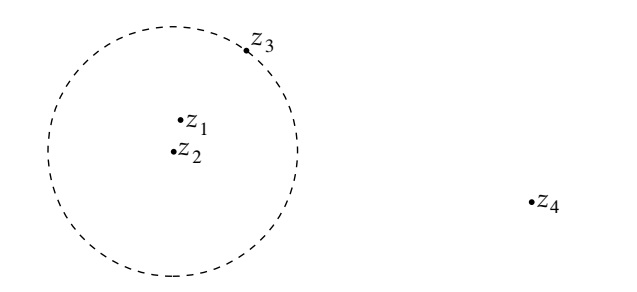
\includegraphics[width=0.6\textwidth]{figure/Fig2.1.jpg}
		\caption{The figure above shows the product of four local operators. The OPE represents the asymptotic behavior as $z_1 \to z_2$ as a series. In this process, a pair of operators at $z_1 , z_2$ is replaced by a single operator at $z_2$.
			The radius of convergence is the distance to other nearest operators, represented by the dashed lines in the figure.    }\label{Fig2.1}
	\end{center}
\end{figure}

The basic objects of study in string perturbation theory are path integral expectation values of products of local operators:    
\begin{equation}
	\left\langle\mathscr{A}_{i_{1}}(z_{1}, \bar{z}_{1}) \mathscr{A}_{i_{2}}(z_{2}, \bar{z}_{2}) \cdots \mathscr{A}_{i_{n}}(z_{n}, \bar{z}_{n})\right\rangle
\end{equation}
where $\mathscr{A}_{i}$ is some basis of the set of local operators. It is very important to understand the behavior of this expectation value in the limit where two of the operators approach each other. A systematic description of this limit is given by the operator product expansion (OPE).    
As shown in Figure \ref{Fig2.1}.    
The OPE states that the product of two local operators close to each other can be approximated to any precision by a sum of local operators:    
\begin{equation}
	\mathscr{A}_{i}(\sigma_{1}) \mathscr{A}_{j}(\sigma_{2})=\sum_{k} c^{k}{}_{i j}(\sigma_{1}-\sigma_{2}) \mathscr{A}_{k}(\sigma_{2}) \:.
	\label{2.2.2}
\end{equation}
This is an operator statement, meaning it holds in a general expectation value:    
\begin{equation}
	\left\langle\mathscr{A}_{i}(\sigma_{1}) \mathscr{A}_{j}(\sigma_{2}) \cdots\right\rangle
	=\sum_{k} c^{k}{}_{i j}(\sigma_{1}-\sigma_{2})\left\langle\mathscr{A}_{k}\left(\sigma_{2}\right) \cdots\right\rangle \label{2.2.3}
\end{equation}
where the distance between $\sigma_{1}, \sigma_{2}$ is smaller than the distance to all other operators. The coefficient function $c^{k}{ }_{i j}(\sigma_{1}-\sigma_{2})$ determines the dependence on the separation, and also depends on $i,j,k$, but is independent of other operators in the expectation value; the dependence on the latter only appears in the expectation value on the right side of (\ref{2.2.3}). These terms are typically arranged in decreasing order of magnitude in the limit $\sigma_{1} \rightarrow \sigma_{2}$.    
Except that the coefficient functions are not simple power series and can be singular as $\sigma_{1} \rightarrow \sigma_{2}$, this is analogous to an ordinary Taylor series.    

We will now use the special properties of free field theory to give a derivation of the OPE for $X^\mu$ theory. In Section 2.9, we will give a derivation for any conformal invariant field theory.    

We have seen that normal products satisfy the equations of motion (\ref{2.1.23}). This indicates that the operator product is a harmonic function of $(z_{1}, \bar{z}_{1})$. A simple result from complex analysis is that a harmonic function is locally the sum of a holomorphic function and an anti-holomorphic function. In particular, it means it is not singular as $z_{1} \rightarrow z_{2}$, and can be freely expanded in a Taylor series in $z_{12}$ and $\bar{z}_{12}$.    
Therefore,    
\begin{align}
	&X^{\mu}(z_{1}, \bar{z}_{1}) X^{v}(z_{2}, \bar{z}_{2})=-\frac{\alpha^{\prime}}{2} \eta^{\mu \nu} \ln \lvert z_{12}\rvert^{2}+ 
	:\mathrel{ X^{v} X^{\mu}(z_{2}, \bar{z}_{2})}:  \nonumber \\
	&\qquad +\sum_{k=1}^{\infty} \frac{1}{k!}\Bigl[(z_{12})^{k}\!
	:\mathrel{X^{v} \partial^{k} X^{\mu}(z_{2}, \bar{z}_{2})}:+
	(\bar{z}_{12})^{k}\!:\mathrel{ X^{v} \bar{\partial}^{k} X^{\mu}(z_{2}, \bar{z}_{2})}:\Bigr] \label{2.2.4}
\end{align}
\begin{tcolorbox}[breakable]
	\begin{remark}
		Here (\ref{2.1.21a}) and    
		\begin{align*}
			&:\mathrel{X^{\mu}(z_{1},\bar{z}_{1}) X^{\nu}(z_{2}, \bar{z}_{2})}:\\
			=&: \mathrel{ X^{\nu} X^{\mu}(z_{2},\bar{z}_{2})}:+\sum_{k=1}^{\infty} \frac{1}{k !}\Bigl[(z_{12})^{k}\!:\mathrel{X^{\nu} \partial^{k} X^{\mu}(z_{2}, \bar{z}_{2})}:+(\bar{z}_{12})^{k}\!:\mathrel{X^{\nu} \bar{\partial}^{k} X^{\mu}(z_{2}, \bar{z}_{2})}:\Bigr]
		\end{align*}
		are used. Because of the equations of motion, the terms with mixed derivatives $\partial \bar{\partial}$ are zero.    
	\end{remark}
\end{tcolorbox}


Equation (\ref{2.2.4}) has the form of an OPE. Like the equation of motion (\ref{2.1.23}) that derived it, this is a statement about operators. For any vacuum expectation value of the product of $X^{\mu}(z_{1},\bar{z}_{1}) X^{v}(z_{2},\bar{z}_{2})$ with fields at other points, its behavior as $z_{1}\to z_{2}$ is an infinite series, where each term is a known function of $z_{12}$ and (or) $\bar{z}_{12}$ multiplied by the expectation value of the local operator that replaces this pair of fields.    

The OPE is usually used as an asymptotic expansion, where the first few terms give the dominant behavior when the separation is very small. Most of our applications will be of this type, and we usually write the OPE as clearly singular terms plus unspecified non-singular remainder terms. Instead of using $=$, we will use "$\sim$" to mean "equal in the sense of differing only by non-singular terms." In fact, the OPE converges in conformal invariant field theories. In certain applications, this is very important to us: it makes it possible to reconstruct the entire theory from the coefficient functions.    
As an example, the radius of convergence of the free field OPE (\ref{2.2.4}) in any given expectation value is equal to the distance from it to the nearest of the other insertions in the path integral, as shown in Figure \ref{Fig2.1}, and the convergence can be proven by standard complex analysis theory.    

Various operators on the right side of the OPE (\ref{2.2.4}) include the product of fields at the same point. In quantum field theory, such products are usually divergent, and thus need to be appropriately truncated and renormalized, but the normal-ordering here makes it well-defined.    
In free field theory, normal-ordering is a convenient way to define composite operators. In interacting field theory, normal-ordering is of little use because composite operators have additional divergences caused by interaction vertices connected to them.    
However, the field theories we are interested in are mostly free field theories, or theories related to free field theories, so more details on normal-ordering are given here.    
Normal-ordering of any number of fields can be defined recursively as    
\begin{align}
	&: \mathrel{ X^{\mu_{1}}(z_{1}, \bar{z}_{1}) \cdots X^{\mu_{n}}(z_{n}, \bar{z}_{n})}: \nonumber \\
	&\qquad\quad =X^{\mu_{1}}(z_{1}, \bar{z}_{1}) \cdots X^{\mu_{n}}(z_{n}, \bar{z}_{n})+\sum \text{subtractions}, \label{2.2.5}
\end{align}
where the subtractions refer to picking one or more pairs of fields from the product of fields and replacing them with $\frac{1}{2} \alpha^{\prime} \eta^{\mu_{i} \mu_{j}} \ln \lvert z_{i j}\rvert^{2}$.    
For example,    
\begin{align}
	&:\mathrel{X^{\mu_{1}}(z_{1}, \bar{z}_{1}) X^{\mu_{2}}(z_{2}, \bar{z}_{2}) X^{\mu_{3}}(z_{3}, \bar{z}_{3})}: = 
	X^{\mu_{1}}(z_{1}, \bar{z}_{1}) X^{\mu_{2}}(z_{2}, \bar{z}_{2}) X^{\mu_{3}}(z_{3}, \bar{z}_{3}) \nonumber \\
	&\qquad+\left(\frac{\alpha^{\prime}}{2} \eta^{\mu_{1} \mu_{2}} \ln \lvert z_{12}\rvert^{2} X^{\mu_{3}}(z_{3}, \bar{z}_{3})+2 \text{ permutations}\right).
	\label{2.2.6}
\end{align}

This definition can be compactly summarized as    
\begin{equation}
	: \mathrel{\mathscr{F}}:=\exp \left(\frac{\alpha^{\prime}}{4} \int \dif^{2} z_{1} \dif^{2} z_{2} \ln \lvert z_{12}\rvert^{2}\: 
	\frac{\delta}{\delta X^{\mu}(z_{1}, \bar{z}_{1})} \frac{\delta}{\delta X_{\mu}(z_{2}, \bar{z}_{2})}\right) \mathscr{F} \:, \label{2.2.7}
\end{equation}
where $\mathscr{F}$ is any functional of $X$.    
This is equivalent to equation (\ref{2.2.5}): the double functional derivative in the exponent contracts each pair of fields, and summing the exponent of multiple pairings cancels out the fractions in the derivative action. An application of this formal expression is to apply the inverse of the exponent on both sides, which gives    
\begin{align}
	\mathscr{F} &=\exp \left(-\frac{\alpha^{\prime}}{4} \int \dif^{2} z_{1} \dif^{2} z_{2} \ln \lvert z_{12}\rvert^{2}\: 
	\frac{\delta}{\delta X^{\mu}(z_{1}, \bar{z}_{1})} \frac{\delta}{\delta X_{\mu}(z_{2}, \bar{z}_{2})}\right):\mathrel{\mathscr{F}}: \nonumber \\
	&=: \mathrel{\mathscr{F}}:+\sum \text {contractions}\:, \label{2.2.8}
\end{align}
where the contractions are the inverse of subtractions: picking one or more pairs of fields from $:\mathrel{\mathscr{F}}:$ and replacing them with $-\frac{1}{2} \alpha^{\prime} \eta^{\mu_{i} \mu_{j}} \ln \lvert z_{i j}\rvert^{2}$.    
For any functionals $\mathscr{F}$ and $\mathscr{G}$ of $X$, their OPE is generated by    
\begin{equation}
	: \mathrel{\mathscr{F}}: :\mathrel{\mathscr{G}}:=: \mathrel{\mathscr{F} \mathscr{G}}:+\sum \text{cross contractions}
\end{equation}
The cross contractions now refer to contracting a field in $\mathscr{F}$ and a field in $\mathscr{G}$ and summing over them. This can also be written as    
\begin{equation}
	: \mathrel{\mathscr{F}}: :\mathrel{\mathscr{G}}:= \exp \left(-\frac{\alpha^{\prime}}{2} 
	\int \dif^{2} z_{1} \dif^{2} z_{2}\: \ln \lvert z_{12}\rvert^{2} \frac{\delta}{\delta X_{F}^{\mu}(z_{1}, \bar{z}_{1})} 
	\frac{\delta}{\delta X_{G \mu}(z_{2}, \bar{z}_{2})}\right): \mathrel{\mathscr{F} \mathscr{G}}: \label{2.2.10}
\end{equation}
where the functional derivatives only act on fields in $\mathscr{F}$ or $\mathscr{G}$ respectively.    
As an example,    
\begin{align}
	&: \mathrel{\partial X^{\mu}(z) \partial X_{\mu}(z)}: : \mathrel{\partial^{\prime} X^{v}(z^{\prime}) \partial^{\prime} X_{v}(z^{\prime})}: \nonumber \\
	&\qquad \qquad \qquad =: \mathrel{\partial X^{\mu}(z) \partial X_{\mu}(z) \partial^{\prime} X^{v}(z^{\prime}) \partial^{\prime} X_{v}(z^{\prime})}: \nonumber\\
	&\qquad \qquad \qquad \qquad \qquad {-}4 \cdot \frac{\alpha^{\prime}}{2}
	(\partial \partial^{\prime} \ln \lvert z-z^{\prime}\rvert^{2}): \mathrel{\partial X^{\mu}(z) \partial^{\prime} X_{\mu}(z^{\prime})}: \nonumber\\
	&\qquad \qquad \qquad \qquad \qquad {+}2 \cdot \eta^{\mu}{ }_{\mu}\left(-\frac{\alpha^{\prime}}{2} \partial \partial^{\prime}
	\ln \lvert z-z^{\prime}\rvert^{2}\right)^{2} \nonumber\\
	&\qquad \qquad \qquad \sim \frac{D \alpha^{\prime 2}}{2(z-z^{\prime})^{4}}-\frac{2 \alpha^{\prime}}{(z-z^{\prime})^{2}}
	: \mathrel{\partial^{\prime} X^{\mu}(z^{\prime}) \partial^{\prime} X_{\mu}(z^{\prime})}: \nonumber\\
	&\qquad \qquad \qquad \qquad \qquad {-}\frac{2 \alpha^{\prime}}{z-z^{\prime}}: \mathrel{\partial^{\prime 2} X^{\mu}\left(z^{\prime}\right) \partial^{\prime} X_{\mu}\left(z^{\prime}\right)}:\:.
	\label{2.2.11}
\end{align}
The second term after the equal sign comes from the four ways to contract a single pair of fields, while the third term comes from the two ways to contract two pairs of fields. In the last line, we write the OPE in standard form by performing a Taylor expansion inside the normal ordering: each operator in each term is at $z'$, and arranged in order of singularity.    

\begin{tcolorbox}[breakable]
	\begin{remark}
		The second term after the equal sign comes from    
		\begin{align*}
			\wick{ : \partial \c1 {X}^{\mu}(z) \partial X_{\mu}(z) : : \partial^{\prime} \c1 {X}^{\nu} (z^{\prime}) \partial^{\prime} X_{\nu}(z^{\prime}) : }
			&=\partial \partial^{\prime}\left(-\frac{\alpha^{\prime}}{2} \eta^{\mu \nu}\ln \lvert z-z^{\prime}\rvert^{2}\right) 
			: \mathrel{\partial X_{\mu}(z) \partial X_{\nu}(z)}: \\
			&=-\frac{\alpha^{\prime}}{2} \Bigl(\partial \partial^{\prime} \ln \lvert z-z^{\prime}\rvert^{2}\Bigr)  
			: \mathrel{\partial X_{\mu}(z) \partial^{\prime} X^{\mu}(z)}:
		\end{align*}
		while the third term comes from
		\begin{align*}
		\wick{ : \partial \c1 {X}^{\mu}(z) \partial \c2 {X}_{\mu}(z) : : \partial^{\prime} \c1 {X}^{\nu}(z^{\prime}) \partial^{\prime} \c2 {X}_{\nu}(z^{\prime}) : } 
			&=\partial \partial^{\prime}\left(-\frac{\alpha^{\prime}}{2} \eta ^{\mu \nu} \ln \lvert z-z^{\prime}\rvert^{2}\right) 
			\partial \partial^{\prime}\left(-\frac{\alpha^{\prime}}{2} \eta_{\mu \nu}\ln \lvert z-z^{\prime}\rvert^{2}\right) \\
			&=\eta^{\mu \nu} \eta_{\mu \nu}\left(-\frac{\alpha^{\prime}}{2} \partial \partial^{\prime}\ln \lvert z- z^{\prime}\rvert ^{2}\right)^{2}
		\end{align*}
		Because $\eta^{\mu \nu} \eta_{\nu\rho}=\delta^{\mu}{}_{\rho}$, so $\eta^{\mu \nu} \eta_{\mu \nu}=\delta^{\mu}{ }_{\mu}=D$, and then using    
		$
		\partial \partial^{\prime} \ln \lvert z-z^{\prime }\vert 
		^{2}= (z-z^{\prime})^{-2}
		$
		and    
		\[
		:\mathrel{\partial X^\mu(z)\partial^\prime X_{\mu}(z^\prime)}:\sim :\mathrel{\partial^\prime X^\mu(z^\prime)\partial^\prime X_\mu(z^\prime)}: 
		+ \:(z-z^\prime):\mathrel{\partial^{\prime 2} X^\mu(z^\prime)\partial^\prime X_\mu(z)}:
		\]
		(\ref{2.2.11}) is obtained.    
	\end{remark}
\end{tcolorbox}


Another important example is    
\begin{equation}
	\mathscr{F}=\me^{\mi k_{1} \cdot X(z, \bar{z})}, \qquad \mathscr{G}=\me^{\mi k_{2} \cdot X(0,0)}
\end{equation}
The variations $\delta / \delta X_{F}^{\mu}$ and $\delta / \delta X_{G}^{\mu}$ yield the factors $\mi k_{1 \mu}$ and $\mi k_{2 \mu}$ respectively, so the general result (\ref{2.2.10}) becomes    
\begin{align}
	:\mathrel{\me^{\mi k_{1} \cdot X(z, \bar{z})}}: : \mathrel{\me^{\mi k_{2} \cdot X(0,0)}}: 
	&=\exp \left(\frac{\alpha^{\prime}}{2} k_{1} \cdot k_{2} \ln |z|^{2}\right) :\mathrel{\me^{\mi k_{1} \cdot X(z, \bar{z})} \me^{\mi k_{2} \cdot X(0,0)}} : \nonumber \\
	&=|z|^{\alpha^{\prime} k_{1} \cdot k_{2}}: \mathrel{ \me^{\mi k_{1} \cdot X(z, \bar{z})} \me^{\mi k_{2} \cdot X(0,0)}}: \:.
	\label{2.2.13}
\end{align}
To derive the OPE, Taylor expansion in the normal ordering gives    
\begin{equation}
	:\mathrel{\me^{\mi k_{1} \cdot X(z, \bar{z})}}: : \mathrel{\me^{\mi k_{2} \cdot X(0,0)}}: 
	=|z|^{\alpha^{\prime} k_{1} \cdot k_{2}}: \mathrel{\me^{\mi(k_{1}+k_{2}) \cdot X(0,0)}[1+O(z, \bar{z})]}: \:.\label{2.2.14}
\end{equation}
\begin{tcolorbox}[breakable]
	\begin{remark}
		The general result (\ref{2.2.10}) here is    
		\begin{align*}
			&:\mathrel{ \me^{i k_{1} \cdot X(z,\bar{z})}}::\mathrel{\me^{\mi k_{2} \cdot X(0,0)}}:\\
			&\quad =\left(1-\frac{\alpha^{\prime}}{2} \int \dif^{2} z_{1} \dif^{2} z_{2}\: \ln \lvert z_{12}\rvert^{2} \frac{\delta}{\delta X_{F}^{\mu}(z_{1},\bar{z}_{1})} \frac{\delta}{\delta X_{G \mu}(z_{2}, \bar{z}_{2})} +\cdots \right):\mathrel{ \me^{\mi k_{1} \cdot X(z, \bar{z})} \me^{\mi k_{2} \cdot X(0,0)}}:\\
			&\quad =:\mathrel{\me^{\mi k_{1} \cdot X(z, \bar{z})} \me^{\mi k_{2} \cdot X(0,0)}}: \\ 
			&\quad \quad \times \left(1 -\frac{\alpha^{\prime}}{2} \int \dif^{2} z_{1} \dif^{2} z_{2}\: \ln \lvert z_{12}\rvert ^{2}
			\times \mi k_{1 \mu} \delta^{2}(z-z_{1}, \bar{z}-\bar{z}_{1}) \mi k_{2}^{\mu} \delta^{2}(0-z_{2}, 0,-\bar{z}_{2})+ \cdots \right)\\
			&\quad =:\mathrel{\me^{\mi k_{1} \cdot X(z, \bar{z})} \me^{\mi k_{2} \cdot X(0,0)}}: 
			\left(1+\frac{\alpha^{\prime}}{2} k_{1} \cdot k_{2} \ln |z|^{2}+\cdots\right)=
			|z|^{\alpha^{\prime} k_{1} \cdot k_{2}}: \mathrel{ \me^{\mi k_{1} \cdot X(z, \bar{z})} \me^{\mi k_{2} \cdot X(0,0)}}: \:.
		\end{align*}
	\end{remark}
\end{tcolorbox}

Note that OPEs such as (\ref{2.2.2}), (\ref{2.2.4}) are non-symmetric with respect to $\sigma_{1}$ and $\sigma_{2}$. These OPEs can be reshaped into a symmetric form by expanding around $(\sigma_{1}+\sigma_{2})/ 2$.    
The coefficient functions in the symmetric form satisfy, under the exchange of two operators:    
\begin{equation}
	c^{k}{}_{ij}(\sigma_{1}-\sigma_{2})_{\mathrm{sym}}= \pm c^{k}{}_{j i}(\sigma_{2}-\sigma_{1})_{\mathrm{sym}} \:,
\end{equation}
where the sign is negative when $\mathscr{A}_{i}$ and $\mathscr{A}_{j}$ are both anti-commuting.    


\section{\texorpdfstring{Ward identities and Noether theorem}{2.3 Ward identities and Noether theorem}}

Worldsheet symmetry plays an important role in string theory.    
In this section, we first derive some general results for symmetry in field theory.    

Consider a field theory in $d$-dimensional spacetime with action $S_\phi$, where $\phi_\alpha(\sigma)$ labels a general field. Suppose it has the symmetry    
\begin{equation} \label{2.3.1}
	\phi_{\alpha}^{\prime}(\sigma)=\phi_{\alpha}(\sigma)+\delta \phi_{\alpha}(\sigma) \:,
\end{equation}
where $\delta \phi_\alpha$ is proportional to an infinitesimal parameter $\epsilon$. The product of the path integral measure and the weight $\exp(-S)$ is invariant:    
\begin{equation} \label{2.3.2}
	[\dif \phi^{\prime}]\: \exp(-S[\phi^{\prime}])=[\dif  \phi] \exp (-S[\phi]) \:.
\end{equation}

In field theory, a continuous symmetry implies the existence of a conserved current (Noether's theorem) and Ward identities (which constrain operator products of the current). To derive these results, consider the field variation    
\begin{equation}\label{2.3.3}
	\phi_{\alpha}^{\prime}(\sigma)=\phi_{\alpha}(\sigma)+\rho(\sigma) \delta \phi_{\alpha}(\sigma)
\end{equation}
This is not a symmetry, but $[\dif \phi]\exp(-S)$ is invariant when $\rho$ is a constant, so its variation must be proportional to $\partial _a \rho$:    
\begin{align}
	&[\dif \phi^{\prime}]\: \exp (-S[\phi^{\prime}]) \nonumber \\
	&\qquad=[\dif \phi] \: \exp (-S[\phi])\left[1+\frac{\mi \epsilon}{2 \pi} \int \dif^{d} \sigma\: 
	g^{1 / 2} j^{a}(\sigma) \partial_{a} \rho(\sigma)+O\left(\epsilon^{2}\right)\right] \label{2.3.4}
\end{align}
The unknown coefficient $j^a(\sigma)$ comes from the variation of the measure and the action.    
Take $\rho$ to be non-zero only in a small region. Outside this region, consider a path integral containing a general insertion "$\cdots$".    
This insertion is invariant under (\ref{2.3.3}):    
\begin{align}
	0 &=\int[\dif \phi^{\prime}]\: \exp (-S[\phi^{\prime}]) \cdots \: - \: \int[\dif \phi] \exp (-S[\phi]) \cdots \nonumber \\
	&=\frac{\mi \epsilon}{2 \pi} \int \dif^{d} \sigma\: 
	g^{1 / 2} j^{a}(\sigma) \partial_{a} \rho(\sigma)+O(\epsilon^2)=\frac{\epsilon}{2 \pi \mi} \int \dif^{d} \sigma \: g^{1 / 2} \rho(\sigma)\left\langle\nabla_{a} j^{a}(\sigma) \cdots\right\rangle
	\label{2.3.5}
\end{align}
thus we have    
\begin{equation}
	\nabla_{a} j^{a}=0 \:.
	\label{2.3.6}
\end{equation}
\begin{tcolorbox}[breakable]
	\begin{proof}
		We use the fact that \( \partial_a (g^{1/2} v^a(c)) = g^{1/2} \nabla_a v^a(c) \) as shown here
		
		\[
		\begin{aligned}
			\text{LHS} = \partial_a (\sqrt{g} v^a) &= (\partial_a \sqrt{g}) v^a + \sqrt{g} \partial_a v^a \\
			&= \frac{1}{2\sqrt{g}} g g^{bc} \partial_a g_{bc} v^a + \sqrt{g} \partial_a v^a \\
			&= \sqrt{g} \left( \frac{1}{2} g^{bc} \partial_a g_{bc} v^a + \partial_a v^a \right)
		\end{aligned}
		\]
		
		For the RHS we find
		
		\[
		\begin{aligned}
			\text{RHS} = \sqrt{g} \nabla_a v^a &= \sqrt{g} \left( \partial_a v^a + \Gamma^a_{ab} v^b \right) \\
			&= \sqrt{g} \left[ \partial_a v^a + \frac{1}{2} (g^{ac} \partial_a g_{cb} + g^{ac} \partial_b g_{ca} - g^{ac} \partial_c g_{ab}) v^b \right] \\
			&= \sqrt{g} \left( \partial_a v^a + \frac{1}{2} g^{ac} \partial_b g_{ca} v^b \right)
		\end{aligned}
		\]
		
		The second and last term of the connection cancel after interchanging the dummy indices \( a \) and \( c \). This is now equal to the LHS.
		
		To derive \eqref{2.3.5} we start from \eqref{2.3.4}, which implies
		
		\[
		\begin{aligned}
			0 &= \frac{\mi \epsilon}{2 \pi}\int d^d \sigma \, g^{1/2} j^a(\sigma) \partial_a \rho(\sigma) \\
			&= -\frac{\mi \epsilon}{2 \pi}\int d^d \sigma \, \partial_a (g^{1/2} j^a(\sigma)) \rho(\sigma) \\
			&= \frac{\epsilon}{2 \pi i}\int d^d \sigma \, g^{1/2} \nabla_a j^a(\sigma) \rho(\sigma)
		\end{aligned}
		\] 
	\end{proof}    
\end{tcolorbox}

To derive Ward identities, let $\rho(\sigma)$ be 1 in region $R$ and 0 outside $R$. Additionally, introduce a general local operator $\mathscr{A}(\sigma_{0})$ at a point $\sigma_{0}$ within the path integral region $R$.    
Inserting arbitrary operators "$\cdots$" outside $R$ gives    
\begin{equation} \label{2.3.7}
	\delta \mathscr{A}(\sigma_{0})+\frac{\epsilon}{2 \pi \mi} \int_{R} \dif^{d} \sigma \: g^{1 / 2} \nabla_{a} j^{a}(\sigma) \mathscr{A}(\sigma_{0})=0 \:.
\end{equation}

\begin{tcolorbox}[breakable]
	\begin{proof}
		Similar to (\ref{2.3.5}), using $\partial_a\rho\big\lvert_{|z|=R}\ne0$ we now have    
		\[
		0=\int [\dif \phi]\:\me^{-S[\phi]}\biggl(\delta\mathscr{A}(\sigma_{0})+\frac{\mi\epsilon}{2\pi}\int \dif^{d}\sigma \: 
		j^{a}(\sigma)\partial_{a}\rho(\sigma)\mathscr{A}(\sigma_{0}) \biggr) \cdots     \:,
		\]
		then using integration by parts, (\ref{2.3.7}) can be obtained.    
	\end{proof}
\end{tcolorbox}
\noindent Equivalently,    
\begin{equation}
	\nabla_{a} j^{a}(\sigma) \mathscr{A}(\sigma_{0})=g^{-1 / 2} \delta^{d}(\sigma-\sigma_{0}) \frac{2 \pi}{\mi \epsilon} \delta \mathscr{A}(\sigma_{0})+\sigma \:\text{total derivative} \:.
	\label{2.3.8}
\end{equation}
Divergence theorem gives    
\begin{equation}
	\int_{\partial R} \dif A\: n_{a} j^{a} \mathscr{A}(\sigma_{0})=\frac{2 \pi}{\mi \epsilon} \delta \mathscr{A}(\sigma_{0}) \:,\label{2.3.9}
\end{equation}
where $\dif A$ is the area element, and $n_{a}$ is the outward normal vector.    
In 2-dimensional flat space, this is    
\begin{equation} \label{2.3.10}
	\oint_{\partial R}(j\dif z-\tilde{\jmath} \dif \bar{z}) \mathscr{A}(z_{0}, \bar{z}_{0})
	=\frac{2 \pi}{\epsilon} \delta \mathscr{A}(z_{0}, \bar{z}_{0})
\end{equation}
Here we have dropped the indices $j \equiv j_{z}$, $\tilde{\jmath} \equiv j_{\bar{z}}$. We use $\tilde{\jmath}$ instead of $\bar{\jmath}$ because $\tilde{\jmath}$ is not the conjugate of $j$.    
The Minkowski density $j_0$ is generally Hermitian, $(j_{z})^{\dagger}=\frac{1}{2}(j_{1}-\mi j_{2})^{\dagger}=j_{z}$.    
\begin{tcolorbox}[breakable]
	\begin{proof}
		The proof of (\ref{2.3.9}) used    
		\[
		\int_{R} \dif^{d} \sigma \: g^{1 / 2} \nabla_{a} j^{a} =\int_{R} \dif ^d \sigma \: \partial_{a}\bigl(g^{1 / 2} j^{a}\bigr) 
		=\int_{\partial R} \dif A\: n_{\alpha} j^{a} \:,
		\]
		Using the two-dimensional Stokes' theorem     $
		\int_{R} \dif^{2}z\: \bigl(\partial_{z} v^{z}+\partial_{\bar{z} } v^{\bar{z}}\bigr)=\mi \oint_{\partial R}(v^{z} \dif \bar{z}-v^{\bar{z}} \dif \bar{z})
		$ (\ref{2.3.10}) is obtained.    
	\end{proof}
\end{tcolorbox}

Importantly, the Noether theorem and Ward identities are local properties, and do not depend on distant boundary conditions, nor on whether they are invariant under the symmetry. In particular, because $\rho(\sigma)$ is only non-zero in $R$, only symmetry transformations in $R$ need to be defined.    

In conformal invariant theories, usually $j_z$ is holomorphic and $j_{\bar{z}}$ is anti-holomorphic. In this case, the currents $(j_z,0)$ and $(0,j_{\bar{z}})$ are separately conserved.    
Thus the integral yields the residue in the OPE:    
\begin{equation}\label{2.3.11}
	\operatorname{Res}_{z \to z_{0}} j(z) \mathscr{A}(z_{0}, \bar{z}_{0})+\overline{\operatorname{Res}}_{\bar{z} \to \bar{z}_{0}} \, \tilde{\jmath}(\bar{z}) \mathscr{A}(z_{0}, \bar{z}_{0})=\frac{1}{\mi \epsilon} \delta \mathscr{A}(z_{0}, \bar{z}_{0})
\end{equation}
Here $\operatorname{Res},\overline{\operatorname{Res}}$ refer to taking the coefficients of $(z-z_{0})^{-1}$ and $(\bar{z}-\bar{z}_{0})^{-1}$ respectively.    

An example: Returning to the massless free scalar field, and consider \emph{spacetime} translations $\delta X^{\mu}=\epsilon a^{\mu}$.    
Under $\delta X^{\mu}(\sigma)=\epsilon \rho(\sigma) a^{\mu}$,    
\begin{align}
	\delta S=\frac{1}{4 \pi \alpha^{\prime}} \int \dif^{2}\sigma\: 2(\delta \partial^{a} X^{\mu}) \partial_{a} X_{\mu} 
	=\frac{\epsilon a_{\mu}}{2 \pi \alpha^{\prime}} \int \dif^{2} \sigma \:\partial^{a} X^{\mu} \partial_{a} \rho \:.
\end{align}
This is equivalent to taking the Noether current in (\ref{2.3.5}) as $j_{a}(\sigma)=a_{\mu} j_{a}^{\mu}$, where    
\begin{equation}
	j_{a}^{\mu}=\frac{\mi}{\alpha^{\prime}} \partial_{a} X^{\mu} \:. \label{2.3.13}
\end{equation}
The OPE of the current and the exponential operator gives    
\begin{subequations} \label{2.3.14}
	\begin{align}
		j^{\mu}(z): \mathrel{\me^{\mi k \cdot X(0,0)}}: &\sim \frac{k^{\mu}}{2 z}: \mathrel{\me^{\mi k \cdot X(0,0)}}:  \:,\label{2.3.14a} \\
		\tilde{\jmath}^{\mu}(\bar{z}):\mathrel{ \me^{\mi k \cdot X(0,0)}}: &\sim \frac{k^{\mu}}{2 \bar{z}}: 
		\mathrel{\me^{\mi k \cdot X(0,0)}}:\:.
		\label{2.3.14b}
	\end{align}
\end{subequations}
\begin{tcolorbox}[breakable]
	\begin{proof}
		Explanation for (\ref{2.3.14a}): from (\ref{2.3.13}) it can be obtained that $j^{\mu}=j_{z}^{\mu}=\frac{\mi}{\alpha^{\prime}} \partial_{z} X^{\mu}$, so    
	\begin{align}
		 \frac{i}{\alpha'} \partial X^\mu(z)
		: \sum_{n=0}^{\infty} \frac{i^n}{n!} (k \cdot X(0))^n : &= \frac{i}{\alpha'} 
		: \sum_{n=0}^{\infty} \frac{i^n}{n!} 
		\, \partial X^\mu(z) (k \cdot X(0))^n : \notag\\[6pt]
		&\sim \frac{i}{\alpha'} 
		: \sum_{n=1}^{\infty} \frac{i^n}{n!} 
		\sum_{i=1}^{n}
		\wick{ \c{\partial X^\mu(z)} (k \cdot \c{X(0)}) }_{i}
		\prod_{j\ne i}(k \cdot X(0))_j : \notag\\[6pt]
		&= \frac{i}{\alpha'} 
		: \sum_{n=1}^{\infty} \frac{i^n}{n!} 
		\, n \, \wick{ \c{\partial X^\mu(z)} (k \cdot \c{X(0)}) }
		(k \cdot X(0))^{n-1} : \notag\\[6pt]
		&= \frac{i}{\alpha'} \left(-\frac{\alpha'}{2}\eta^{\mu\nu}\partial\ln(z\bar{z})\right)k_{\nu} 
		: \sum_{n=1}^{\infty} \frac{i^n}{(n-1)!} 
		(k \cdot X(0))^{n-1} : \notag\\[6pt]
		&= \frac{i}{\alpha'} 
		\left(-\frac{\alpha'}{2} \frac{k^\mu}{z} \right)
		: \sum_{n=1}^{\infty} \frac{i^n}{(n-1)!} (k \cdot X(0))^{n-1} : \notag\\[6pt]
		&= \frac{k^\mu}{2z} : e^{ik \cdot X(0)} :.\label{ope: derivX-exp}
	\end{align}
	Alternatively, we can use
	\begin{equation}
		:F::G:
		=
		\exp\!\left(
		-\frac{\alpha'}{2}
		\int d^2 z_1 d^2 z_2 \,
		\log |z_{12}|^2\,
		\frac{\delta}{\delta X_F^\mu(z_1,\bar z_1)}
		\frac{\delta}{\delta X_{G\mu}(z_2,\bar z_2)}
		\right)
		:FG: .
	\end{equation}
	
	This gives
	\begin{align}
		:\frac{i}{\alpha'}\partial X^\mu(z)::e^{ik\cdot X(w,\bar w)}:
		&=
		\exp\!\left(
		-\frac{\alpha'}{2}
		\int d^2 z_1 d^2 z_2\,
		\log |z_{12}|^2\,
		\frac{\delta}{\delta X_F^\mu(z_1,\bar z_1)}
		\frac{\delta}{\delta X_{G\mu}(z_2,\bar z_2)}
		\right)\notag\\
		&\qquad\times:\frac{i}{\alpha'}\partial X^\mu(z)e^{ik\cdot X(w,\bar w)}:
		\\[1ex]
		&=
		:\frac{i}{\alpha'}\partial X^\mu(z)e^{ik\cdot X(w,\bar w)}:
		\nonumber\\
		&\quad
		-\frac{i}{2}
		:
		\int d^2 z_1 d^2 z_2\,
		\log |z_{12}|^2
		\frac{\delta(\partial X^\mu(z))}{\delta X_F^\mu(z_1,\bar z_1)}
		\frac{\delta(e^{ik\cdot X(w,\bar w)})}{\delta X_{G\mu}(z_2,\bar z_2)}
		:
		\nonumber\\[1ex]
		&=
		:\frac{i}{\alpha'}\partial X^\mu(z)e^{ik\cdot X(w,\bar w)}:
		\nonumber\\
		&\quad
		+\frac{i}{2}
		:
		\int d^2 z_1 d^2 z_2\,
		\log |z_{12}|^2\,
		\partial\!\left(
		\delta^\mu_{\ \alpha}\delta^2(z_1,z)
		\right)
		ik^\alpha \delta^2(z_2,w)
		e^{ik\cdot X(w,\bar w)}
		:
		\nonumber\\[1ex]
		&=
		:\frac{i}{\alpha'}\partial X^\mu(z)e^{ik\cdot X(w,\bar w)}:
		\nonumber\\
		&\quad
		+\frac{k^\mu}{2}
		:
		\partial\!\left(
		\int d^2 z_1 d^2 z_2\,
		\log |z_{12}|^2
		\delta^2(z_1,z)\delta^2(z_2,w)
		e^{ik\cdot X(w,\bar w)}
		\right)
		:
		\nonumber\\[1ex]
		&=
		:\frac{i}{\alpha'}\partial X^\mu(z)e^{ik\cdot X(w,\bar w)}:
		+
		\frac{k^\mu}{2}
		:
		\partial\!\left(
		\log |z-w|^2
		e^{ik\cdot X(w,\bar w)}
		\right)
		:
		\nonumber\\[1ex]
		&=
		:\frac{i}{\alpha'}\partial X^\mu(z)e^{ik\cdot X(w,\bar w)}:
		+
		\frac{k^\mu}{2(z-w)}
		:
		e^{ik\cdot X(w,\bar w)}
		: .
	\end{align}
	where we used the fact that $z_1\ne z_2$ to drop higher order terms. Therefore
	\begin{equation}
		:j^\mu(z)::e^{ik\cdot X(w,\bar w)}:
		\sim
		\frac{k^\mu}{2(z-w)}
		:e^{ik\cdot X(w,\bar w)}: .
	\end{equation}
	QED.
	\end{proof}
\end{tcolorbox}

Another example: worldsheet translations $\delta \sigma^{a}=\epsilon v^{a}$, then $\delta X^{\mu}=-\epsilon v^{a} \partial_{a} X^{\mu}$, the Noether current is    
\begin{subequations}
	\begin{align}
		j_{a}  &=\mi v^{b} T_{a b} \:, \label{2.3.15a} \\
		T_{a b}&=-\frac{1}{\alpha^{\prime}}:\mathrel{\biggl(\partial_{a} X^{\mu} \partial_{b} X_{\mu}-\frac{1}{2} \delta_{a b} \partial_{c} X^{\mu} \partial^{c} X_{\mu}\biggr)}: \:.
		\label{2.3.15b}
	\end{align}
\end{subequations}

 \begin{tcolorbox}[breakable]
\begin{proof}
	Consider a local worldsheet translation $\delta \sigma^{a} = \epsilon^{a}(\sigma)$. The corresponding variation of the scalar field is:
	$$ \delta X^{\mu} = -\epsilon^{a}(\sigma) \partial_{a} X^{\mu} $$
	The variation of the Polyakov action (in conformal gauge) is given by:
	\begin{align*}
		\delta S &= \frac{1}{4\pi \alpha'} \int d^{2} \sigma \, 2\partial_{b} (\delta X^{\mu}) \partial^{b} X_{\mu} \\
		&= -\frac{1}{2\pi \alpha'} \int d^{2} \sigma \, \partial_{b} (\epsilon^{a} \partial_{a} X^{\mu}) \partial^{b} X_{\mu} \\
		&= -\frac{1}{2\pi \alpha'} \int d^{2} \sigma \left[ (\partial_{b} \epsilon^{a}) \partial_{a} X^{\mu} \partial^{b} X_{\mu} + \epsilon^{a} (\partial_{b} \partial_{a} X^{\mu} \partial^{b} X_{\mu}) \right]
	\end{align*}
	Using the identity $\partial_{a} (\partial_{c} X^{\mu} \partial^{c} X_{\mu}) = 2 \partial_{b} \partial_{a} X^{\mu} \partial^{b} X_{\mu}$, we rewrite the second term:
	$$ \delta S = -\frac{1}{2\pi \alpha'} \int d^{2} \sigma \left[ (\partial_{b} \epsilon^{a}) \partial_{a} X^{\mu} \partial^{b} X_{\mu} + \frac{1}{2} \epsilon^{a} \partial_{a} (\partial_{c} X^{\mu} \partial^{c} X_{\mu}) \right] $$
	Performing integration by parts on the second term (and assuming $\epsilon^a$ vanishes at infinity):
	$$ \int d^{2} \sigma \, \epsilon^{a} \partial_{a} (\partial_{c} X^{\mu} \partial^{c} X_{\mu}) = - \int d^{2} \sigma (\partial_{a} \epsilon^{a}) (\partial_{c} X^{\mu} \partial^{c} X_{\mu}) $$
	Substituting $\partial_{a} \epsilon^{a} = \delta^{b}_{a} \partial_{b} \epsilon^{a}$ allows us to factor out the derivative of the parameter:
	\begin{align*}
		\delta S &= -\frac{1}{2\pi \alpha'} \int d^{2} \sigma \left[ (\partial_{b} \epsilon^{a}) \partial_{a} X^{\mu} \partial^{b} X_{\mu} - \frac{1}{2} (\partial_{b} \epsilon^{a}) \delta^{b}_{a} (\partial_{c} X^{\mu} \partial^{c} X_{\mu}) \right] \\
		&= \frac{1}{2\pi} \int d^{2} \sigma (\partial_{b} \epsilon^{a}) \left[ -\frac{1}{\alpha'} \left( \partial_{a} X^{\mu} \partial^{b} X_{\mu} - \frac{1}{2} \delta^{b}_{a} \partial_{c} X^{\mu} \partial^{c} X_{\mu} \right) \right]
	\end{align*}
	By the definition of the Noether current $\delta S = \frac{1}{2\pi} \int d^2\sigma (\partial^b \epsilon^a) j_{ab}$, we identify:
	$$ T_{ab} = -\frac{1}{\alpha'} \left( \partial_{a} X^{\mu} \partial_{b} X_{\mu} - \frac{1}{2} \delta_{ab} \partial_{c} X^{\mu} \partial^{c} X_{\mu} \right) $$
	The current for a translation $v^a$ is then $j_a = iv^b T_{ab}$.
\end{proof}
 \end{tcolorbox}


\section{\texorpdfstring{Conformal invariance}{2.4 Conformal invariance}}

The energy-momentum tensor (\ref{2.3.15b}) is traceless: $T_a{}^a=0$.    
In complex coordinates using \eqref{matrix-metric}, we have: 
\begin{equation}
	g^{ab}T_{ab}=\underbrace{g^{zz}}_{=0}T_{zz}+2g^{z\bar{z}}T_{z\bar{z}}+\underbrace{g^{\bar{z}\bar{z}}}_{=0}T_{\bar{z}\bar{z}}\implies T_{z \bar{z}}=0\:. \label{2.4.1}
\end{equation}
The conservation law $\partial^a T_{ab}=0$ implies that in any theory with $T_a{}^a=0$    
\begin{equation}
	\bar{\partial} T_{z z}=\partial T_{\bar{z} \bar{z}}=0 \:. \label{2.4.2}
\end{equation}
Therefore    
\begin{equation}
	T(z) \equiv T_{z z}(z)\:, \qquad \tilde{T}(\bar{z}) \equiv T_{\bar{z} \bar{z}}(\bar{z}) \label{2.4.3}
\end{equation}
are holomorphic and anti-holomorphic respectively.    
For massless free scalars    
\begin{equation}\label{2.4.4}
	T(z)=-\frac{1}{\alpha^{\prime}}: \mathrel{\partial X^{\mu} \partial X_{\mu}}: \:, \qquad 
	\tilde{T}(\bar{z})=-\frac{1}{\alpha^{\prime}}:\mathrel{ \bar{\partial} X^{\mu} \bar{\partial} X_{\mu}}: \:,
\end{equation}
according to the equations of motion, they are indeed holomorphic and anti-holomorphic.    


The tracelessness of $T_{ab}$ implies a much larger symmetry.    
The currents    
\begin{equation}
	j(z)=\mi v(z) T(z) \:, \qquad \tilde{\jmath}(\bar{z})=\mi v(z)^{*} \tilde{T}(\bar{z}) \label{2.4.5}
\end{equation}
are conserved for holomorphic $v(z)$.    
\begin{tcolorbox}[breakable]
	\begin{proof}
		\text{Denote } $j_{z}=i v^{z} T_{z z}$, $j_{\bar{z}}=i v^{\bar{z}} T_{\bar{z} \bar{z}}$.    
		\text{So } $
		\nabla_{a} j^{a}= \bar{\partial} j_{z}+\partial j_{\bar{z}}=0$.    
	\end{proof}    
\end{tcolorbox}
For free scalar theory, the OPE is obtained    
\begin{equation} \label{2.4.6}
	T(z) X^{\mu}(0) \sim \frac{1}{z} \partial X^{\mu}(0), \quad \tilde{T}(\bar{z}) X^{\mu}(0) \sim \frac{1}{\bar{z}} \bar{\partial} X^{\mu}(0)
\end{equation}
% \begin{proof}
	% $$
	% T(z)=-\frac{1}{\alpha^{\prime}}: \partial X^{\mu} \partial X_{\mu}:
	% $$
	% $$
	% -\frac{1}{\alpha^{\prime}}: \partial X^{\mu} \partial X_{\mu}: X^{\nu}(0)=-\frac{1}{\alpha^{\prime}}: \partial X^{\mu} \partial X_{\mu}(z) X^{\nu}(0):\sim \frac{1}{z} \partial X_{\mu} (0)
	% $$
	% \end{proof}
then the Ward identity gives the transformation    
\begin{equation}\label{2.4.7}
	\delta X^{\mu}=-\epsilon v(z) \partial X^{\mu}-\epsilon v(z)^{*} \bar{\partial} X^{\mu}
\end{equation}
This is the infinitesimal coordinate transformation $z^{\prime}=z+\epsilon v(z)$.    
The finite transformation is    
\begin{equation} \label{2.4.8}
	X^{\prime \mu}\left(z^{\prime}, \bar{z}^{\prime}\right)=X^{\mu}(z, \bar{z}), \quad \text{where }z^{\prime}=f(z) \:.
\end{equation}
(\ref{2.4.8}) is called a \emph{conformal transformation}.    
\begin{tcolorbox}[breakable]
	Proof for (\ref{2.4.7}): from (\ref{2.3.11})    
	$$
	\frac{1}{\mi \epsilon} \delta X^{\mu}=\operatorname{Res}_{z \rightarrow z_{0}} \mi v^{z} T(z) X^{\mu}(z_{0},\bar{z}_{0})+
	\overline{\operatorname{Res}}_{\bar{z} \rightarrow \bar{z}_{0}} \mi v^{\bar{z}} \bar{T}(\bar{z}) X^{\mu}(z_{0},\bar{z}_{0})
	$$
	Using (\ref{2.4.6}), (\ref{2.4.7}) is obtained.    
\end{tcolorbox}


Conformal invariance should not be confused with diff invariance. We are in flat space, with no independent metric field used for variation.    
So the transformation $z\to z^\prime$ really changes the distance between points. We don't just happen to have this invariance; it is a non-trivial statement about the dynamics. For the scalar action (\ref{2.1.10}), the conformal transformations of $\partial$ and $\bar{\partial}$ exactly cancel out the conformal transformation of $\dif^2 z$. The mass term $m^{2} X^{\mu} X_{\mu}$ is not conformal invariant.    
Ultimately, there must be a close connection with the diff$\times$ Weyl symmetry of the Polyakov string.    

Consider the special case    
\begin{equation}\label{2.4.9}
	z^{\prime}=\zeta z \:,
\end{equation}
$\zeta$ is any complex number.    
The phase of $\zeta$ is the rotation of the system, while its magnitude is the rescaling of the size of the system. This scale invariance is often viewed as an approximate symmetry in particle physics, and statistical systems near critical points are also described by scale-invariant field theories.    

For generalized conformal transformations, examine its effect on $\dif s^{2}=g_{ab}\dif\sigma^{a} \dif \sigma^{b}=\dif z \dif \bar{z}$    
\begin{equation}
	\dif s^{\prime 2}=\dif z^{\prime} \dif \bar{z}^{\prime}=\frac{\partial z^{\prime}}{\partial z} \frac{\partial \bar{z}^{\prime}}{\partial \bar{z}} \dif z \dif \bar{z} \:.
\end{equation}
As shown in Figure \ref{fig2.2}, we see that the conformal transformation turns an infinitesimal square into an infinitesimal square but adjusts its size. An anti-holomorphic function $z^{\prime}=f(z)^{*}$ has the same property but changes the orientation.    
Most systems invariant under (\ref{2.4.9}) are usually invariant under the much larger conformal invariance. A theory with this invariance is called a \emph{conformal field theory} (CFT).    
\begin{figure}[!htbp]
	\begin{center}
		\includegraphics[width=0.8\textwidth]{figure/fig2.2.jpg}
		\caption{(a) Two-dimensional region. (b) The effect of the special conformal transformation (\ref{2.4.9}). (c) The effect of a more general conformal transformation.    } \label{fig2.2}
	\end{center}
\end{figure}

\subsection*{Conformal Invariance and the OPE}

Conformal invariance imposes a strong constraint on the form of the OPE, especially the OPE of the energy-momentum tensor. Examine the OPE of $T$ and a general operator $\mathscr{A}$.    
Because $T(z)$ and $\tilde{T}(\bar{z})$ are (anti-)holomorphic except at coincidence points, the corresponding coefficient functions must also have this property. The OPE of $T$ and $\mathscr{A}$ is thus a Laurent expansion, where the terms are integer powers of $z$, though the power may be negative. Furthermore, all singular terms are determined by the conformal transformation of $\mathscr{A}$. To see this, we write a general expansion for the singularity    
\begin{equation}\label{2.4.11}
	T(z) \mathscr{A}(0,0) \sim \sum_{n=0}^{\infty} \frac{1}{z^{n+1}} \mathscr{A}^{(n)}(0,0)
\end{equation}
similar for $\tilde{T}$; the operator coefficient $\mathscr{A}^{(n)}$ is left to be determined later.    
Under an infinitesimal conformal transformation $z^{\prime}=z+\epsilon v(z)$, when the $z^{-n-1}$ term in the $T \mathscr{A}$ OPE is multiplied by the $z^n$ term in $v(z)$, a simple pole appears in $v(z) T(z) \mathscr{A}(0,0)$.    
Therefore the (\ref{2.3.11}) form of the Ward identity implies    
\begin{equation}\label{2.4.12}
	\delta \mathscr{A}(z, \bar{z})=-\epsilon \sum_{n=0}^{\infty} \frac{1}{n !}\Bigl[\partial^{n} v(z) \mathscr{A}^{(n)}(z, \bar{z})+\bar{\partial}^{n} v(z)^{*} \tilde{\mathscr{A}}^{(n)}(z, \bar{z})\Bigr]
\end{equation}
\begin{tcolorbox}[breakable]
	\begin{proof}
		Under the coordinate transformation $z^a \to z^a + \epsilon v^a(z)$, where $a$ labels $(z,\bar z)$.
		We determine $\delta \mathscr{A}$ using the residues theorem from \eqref{2.3.11}, expanding $v(z)$ and $\bar v(\bar z)$ in Taylor series:
		\begin{align}
			\delta \mathscr{A}(z_0,\bar z_0)
			&= i\epsilon \frac{1}{2\pi i} \oint_C j(z)\mathscr{A}
			+ i\epsilon \frac{1}{2\pi i} \oint_C \bar j(\bar z)\mathscr{A} \notag\\
			&= i\epsilon \frac{1}{2\pi i} \oint_C i v(z) T(z)\mathscr{A}
			+ i\epsilon \frac{1}{2\pi i} \oint_C i \bar v(\bar z)\bar T(\bar z)\mathscr{A} \notag\\
			&= -\frac{\epsilon}{2\pi i} \oint_C 
			\sum_{k=0}^{\infty} \frac{(z-z_0)^k}{k!}\,\partial^k v(z_0)
			\sum_{n=0}^{\infty} \frac{\mathscr{A}^{(n)}(z_0,\bar z_0)}{(z-z_0)^{n+1}} \notag\\
			&\quad -\frac{\epsilon}{2\pi i} \oint_C 
			\sum_{k=0}^{\infty} \frac{(\bar z-\bar z_0)^k}{k!}\,\bar\partial^k \bar v(\bar z_0)
			\sum_{n=0}^{\infty} \frac{\bar{\mathscr{A}}^{(n)}(z_0,\bar z_0)}{(\bar z-\bar z_0)^{n+1}} \notag\\
			&= -\epsilon \sum_{n=0}^{\infty} \frac{1}{n!}\,\partial^n v(z_0)\,\mathscr{A}^{(n)}(z_0,\bar z_0)
			-\epsilon \sum_{n=0}^{\infty} \frac{1}{n!}\,\bar\partial^n \bar v(\bar z_0)\,\bar{\mathscr{A}}^{(n)}(z_0,\bar z_0).
		\end{align}
		QED.
	\end{proof}
\end{tcolorbox}
Thus the operator $\mathscr{A}^{(n)}$ is determined by the conformal transformation of $\mathscr{A}$.    
It is convenient to take operators that are eigenstates under the rigid transformation (\ref{2.4.9}) as a basis    
\begin{equation}\label{2.4.13}
	\mathscr{A}^{\prime}(z^{\prime}, \bar{z}^{\prime})=\zeta^{-h} \bar{\zeta}^{-\tilde{h}} \mathscr{A}(z, \bar{z}) \:.
\end{equation}
$(h, \tilde{h})$ are called weights. $h+ \tilde{h}$ is the dimension of $\mathscr{A}$, which determines its behavior under rescaling, and $h- \tilde{h}$ is the spin, which determines its behavior under rotation.    
The derivative $\partial_z$ raises $h$ by one, $\partial_{\bar{z}}$ raises $\tilde{h}$ by one. The Ward identity for the transformation (\ref{2.4.13}) and the Ward identity for translation $\delta \mathscr{A}=-\epsilon v^{a} \partial_{a} \mathscr{A}= -\epsilon v(z)\,\partial \mathscr{A} - \epsilon\bar v(\bar z)\,\bar\partial \mathscr{A}$ determine the part of the OPE    
\begin{equation}\label{2.4.14}
	T(z) \mathscr{A}(0,0)=\cdots+\frac{h}{z^{2}} \mathscr{A}(0,0)+\frac{1}{z} \partial \mathscr{A}(0,0)+\cdots
\end{equation}
Similarly for $\tilde{T}$.    
\begin{tcolorbox}[breakable]
	\begin{proof}
		We wish to determine the coefficients $\mathscr{A}^{(n)}(w)$ in the OPE
		\begin{equation}
			T(z)\mathscr{A}(w) \sim \sum_{n=0}^{\infty} \frac{\mathscr{A}^{(n)}(w)}{(z-w)^{n+1}} .
		\end{equation}
		
		for an operator that satisfies $\mathscr{A}'(z')=\zeta^{-h}\mathscr{A}(z)$ under a conformal transformation $z'=\zeta z$.
		Let us first go to an infinitesimal rescaling $\zeta=1+\epsilon$. Then $z'=(1+\epsilon)z=z+\epsilon v(z)$ for $v(z)=z$. From \eqref{2.4.12}, we have then that the only non-vanishing terms are
		\begin{align}
			\delta \mathscr{A}(z) &= -\epsilon \sum_{n=0}^{\infty} \frac{1}{n!}\partial^n v(z)\, \mathscr{A}^{(n)}(z) \\
			&= -\epsilon \left( \frac{1}{0!}\partial^0 v(z)\,\mathscr{A}^{(0)}(z) + \frac{1}{1!}\partial v(z)\,\mathscr{A}^{(1)}(z) \right) \\
			&= -\epsilon \left( z\mathscr{A}^{(0)}(z) + \mathscr{A}^{(1)}(z) \right) .
		\end{align}
		
		But we also have the transformation law
		\begin{equation}
			\mathscr{A}'(z') = \zeta^{-h} \mathscr{A}(z) = (1+\epsilon)^{-h} \mathscr{A}(z) = (1-h\epsilon)\mathscr{A}(z) .
		\end{equation}
		
		But we also have, to first order in $\epsilon$,
		\begin{equation}
			\mathscr{A}'(z') = \mathscr{A}'(z+\epsilon z) = \mathscr{A}'(z) + \epsilon z \partial \mathscr{A}'(z) = \mathscr{A}'(z) + \epsilon z \partial \mathscr{A}(z) .
		\end{equation}
		
		Therefore
		\begin{equation}
			(1-h\epsilon)\mathscr{A}(z) = \mathscr{A}'(z) + \epsilon z \partial \mathscr{A}(z) .
		\end{equation}
		
		and thus
		\begin{equation}
			\delta \mathscr{A}(z) = \mathscr{A}'(z) - \mathscr{A}(z) = -\epsilon z \partial \mathscr{A}(z) - h\epsilon \mathscr{A}(z) .
		\end{equation}
		
		Comparing both results for $\delta \mathscr{A}(z)$ we see that
		\begin{equation}
			\mathscr{A}^{(0)}(z) = \partial \mathscr{A}(z)
			\qquad \text{and} \qquad
			\mathscr{A}^{(1)}(z) = h\mathscr{A}(z) .
		\end{equation}
		
		which shows \eqref{2.4.14}.
		
		Similarly, under a translation $z'=z+\epsilon=z+\epsilon v(z)$ for $v(z)=1$, the only non-vanishing term in \eqref{2.4.12} is
		\begin{equation}
			\delta \mathscr{A}(z) = -\epsilon \partial^0 v(z)\, \mathscr{A}^{(0)}(z) = -\epsilon \mathscr{A}^{(0)}(z) .
		\end{equation}
		
		Comparing this with $\delta \mathscr{A}(z)=-\epsilon v(z)\partial \mathscr{A}(z)=-\epsilon \partial \mathscr{A}(z)$ we recover
		\begin{equation}
			\mathscr{A}^{(0)}(z) = \partial \mathscr{A}(z) .
		\end{equation}
	\end{proof}
\end{tcolorbox}

Particularly important are tensor operators or primary fields $\mathcal{O}$.    
The general conformal transformation acting on them gives    
\begin{equation}
	\mathcal{O}^{\prime}(z^{\prime}, \bar{z}^{\prime})= (\partial_{z} z^{\prime})^{-h}(\partial_{\bar{z}} \bar{z}^{\prime})^{-\tilde{h}} \mathcal{O}(z, \bar{z}) \:.
\end{equation}
The OPE (\ref{2.4.11}) reduces to    
\begin{equation}\label{2.4.16}
	T(z) \mathcal{O}(0,0)=\frac{h}{z^{2}} \mathcal{O}(0,0)+\frac{1}{z} \partial \mathcal{O}(0,0)+\cdots \:,
\end{equation}
The more singular terms in the general OPE (\ref{2.4.14}) are gone.    
\begin{tcolorbox}[breakable]
\begin{remark}
	A local operator $\mathscr A$ is primary if its OPE with the stress tensor truncates at second order:
	\begin{equation}
		T(z)\,\mathscr A(w) \sim 
		\frac{h\,\mathscr A(w)}{(z-w)^2}
		+ \frac{\partial \mathscr A(w)}{z-w}
		+ \text{regular},
	\end{equation}
	and similarly for $\bar T(\bar z)$. In particular, no higher-order singularities are allowed. 
	However, from \eqref{2.4.22} we see that the $T(z)T(w)$ OPE contains a $(z-w)^{-4}$ term, arising from the central extension. This violates the primary condition, and hence $T$ is not a primary operator (but rather quasi-primary).
\end{remark}
\end{tcolorbox}
Take free $X^\mu$ CFT as an example once again. Some weights of typical operators are    
\begin{equation}
	\left.\begin{array}{llll}
		X^{\mu} & (0,0) \:, & \partial X^{\mu} & (1,0) \:, \\
		\bar{\partial} X^{\mu} & (0,1) \:, & \partial^{2} X^{\mu} & (2,0)  \:,\\
		: \mathrel{\me^{\mi k \cdot X}}: & \left(\frac{\alpha^{\prime} k^{2}}{4}, \frac{\alpha^{\prime} k^{2}}{4}\right) \:.
	\end{array}\right\} \label{2.4.17}
\end{equation}
\begin{tcolorbox}[breakable]
	\begin{remark}
		We can read off conformal weight $h=\bar{h}=0$ of $X^{\mu}$ from \eqref{2.4.6}, yet its two-point function in \eqref{2.1.21b} does not take the standard form
		\begin{align*}
			\ev{\phi_1(z_1,\bar z_1)\phi_2(z_2,\bar{z}_2)}=\frac{C_{12}}{(z_1-z_2)^{h}(\bar{z}_1-\bar{z}_2)^{\bar{h}}}.
		\end{align*}
		Therefore, $X^{\mu}$ is not a primary field. Nevertheless, although $X^{\mu}$ itself is not primary, the operator $:e^{ik\cdot X(z,\bar z)}:$ is. Indeed, its two-point function from \eqref{2.2.13} takes the expected form:
		\begin{align}
			\big\langle :e^{ik\cdot X(z,\bar z)}:\, :e^{ip\cdot X(w,\bar w)}:\big\rangle&=|z-w|^{\alpha' k\cdot p}\big\langle :e^{ik\cdot X(z,\bar z)}e^{ip\cdot X(w,\bar w)}:\big\rangle\nonumber\\
			&= |z-w|^{\alpha' k\cdot p} \, \delta^{(D)}(\vec k+\vec p)\nonumber \\
			%\big\langle :e^{ik\cdot X(z,\bar z)}:\, :e^{-ik\cdot X(w,\bar w)}:\big\rangle
			&= \frac{1}{|z-w|^{\alpha' k^2}}
		\end{align}
		where in the second line we have set $\vec p=-\vec k$ and utilized,
		\begin{align*}
			\bra{0;0}e^{i(k_1+k_2)\cdot x}e^{\alpha'(k_1\ln|z|^2+k_2\ln|w|^2)\cdot p}\ket{0;0}&=\bra{0;0}e^{i(k_1+k_2)\cdot x}\ket{0;0}=\braket{0;0}{0;k_1+k_2}\nonumber\\
			&=\delta(\vec{k}_1+\vec{k}_2).
		\end{align*}
	\end{remark}
\end{tcolorbox}
Except for $\partial^{2} X^{\mu}$, all quantities transform as tensors. More generally, general products of exponentials and derivatives    
\begin{equation}
	:\mathrel{\Bigl({\textstyle \prod_{i}} \partial^{m_{i}} X^{\mu_{i}}\Bigr)\Bigl({\textstyle \prod_{j}} \bar{\partial}^{n_{j}} X^{v_{j}}\Bigr) \me^{\mi k \cdot X} }:
\end{equation}
have weights    
\begin{equation}
	\biggl(\frac{\alpha^{\prime} k^{2}}{4}+ {\textstyle\sum_{i}} m_{i}, \frac{\alpha^{\prime} k^{2}}{4}+\textstyle{\sum_{j}} n_{j}\biggr) \:.
	\label{2.4.19}
\end{equation}

For any pair of operators, applying rigid transformations, rescaling, and rotation on both sides of the OPE completely determines the dependence of the coefficient function on $z$    
\begin{equation}\label{2.4.20}
	\mathscr{A}_{i}(z_{1}, \bar{z}_{1}) \mathscr{A}_{j}(z_{2}, \bar{z}_{2})=\sum_{k} z_{12}^{h_{k}-h_{i}-h_{j}} 
	\bar{z}_{12}^{\tilde{h}_{k}-\tilde{h}_{i}-\tilde{h}_{j} }c^{k}{}_{i j} \mathscr{A}_{k}(z_{2}, \bar{z}_{2}) \:,
\end{equation}
where $c^k{}_{ij}$ are now constants. In all interesting cases, the weights appearing on the right side of the OPE (\ref{2.4.20}) have a lower bound, so the singularity in the operator product is constrained.    
More general conformal transformations impose further constraints on the OPE: they completely determine the OPE of all fields with the OPE of primary fields.    

Note that in general, the conformal transformation properties of normal products are not determined by the naive transformation of the product.    
For example, the transformation rule (\ref{2.4.7}) for $X^\mu$ would naively imply    
\begin{equation}
	\delta \me^{\mi k \cdot X}=-\epsilon v(z) \partial \me^{\mi k \cdot X}-\epsilon v(z)^{*} \bar{\partial} \me^{\mi k \cdot X} \quad \text { (naive) }
\end{equation}
making it a (0,0) tensor.    
Since defining the operator product at a point requires renormalization, this modification is a quantum effect. In particular, it enters here because the subtraction of $\ln \lvert z_{12}\rvert^{2}$ in $\mathrel{:\::}$ has a clear dependence on the coordinate system.    

\subsection*{Conformal Properties of the Energy-Momentum Tensor}
The OPE of the energy-momentum tensor with itself is obtained from (\ref{2.2.11})    
\begin{equation}\label{2.4.22}
	\begin{aligned}
		T(z) T(0) &=\frac{\eta^{\mu}{}_{\mu}}{2 z^{4}}-\frac{2}{\alpha^{\prime} z^{2}}: \mathrel{\partial X^{\mu}(z) \partial X_{\mu}(0)}:+ 
		: \mathrel{T(z) T(0)}: \\
		& \sim \frac{D}{2 z^{4}}+\frac{2}{z^{2}} T(0)+\frac{1}{z} \partial T(0)
	\end{aligned}
\end{equation}
A similar result exists for $\tilde{T}$.    
The OPE of $T(z) \tilde{T}(\bar{z}^{\prime})$ must be non-singular; it cannot have a singularity at $(z-z^{\prime})$ because it is anti-holomorphic in $z^{\prime}$ over a non-zero interval. Similarly, it cannot have a singularity at $(\bar{z}-\bar{z}^{\prime})$. The same result holds for any OPE of a holomorphic operator and an anti-holomorphic operator.    

Thus $T$ is \emph{not} a tensor. And the OPE (\ref{2.4.22}) implies the transformation rule    
\begin{equation}
	\epsilon^{-1} \delta T(z)=-\frac{D}{12} \partial_{z}^{3} v(z)-2 \partial_{z} v(z) T(z)-v(z) \partial_{z} T(z) \:.
	\label{2.4.23}
\end{equation}
In a general CFT, the transformation of $T(z)$ is    
\begin{equation}\label{2.4.24}
	\epsilon^{-1} \delta T(z)=-\frac{c}{12} \partial_{z}^{3} v(z)-2 \partial_{z} v(z) T(z)-v(z) \partial_{z} T(z) \:,
\end{equation}
where $c$ is a constant called the central charge. The central charge of a free scalar field is 1. For $D$ free scalar fields it is $D$. The transformation (\ref{2.4.24}) is the most general form, which is linear in $v$. This is consistent with the symmetry of the $TT$ OPE, where the three $z$ subscripts are required by rigid transformation, rescaling and rotation invariance.    
Scaling, rotation and translation symmetries determine the coefficients of the 2nd and 3rd terms. Furthermore, by examining the commutator of two such transformations, it can be proven that $\partial_{a} c=0$. This is a general result in quantum field theory. Operators that are independent of position must be $c$-numbers. The corresponding $TT$ OPE is    
\begin{equation}\label{2.4.25}
	T(z) T(0) \sim \frac{c}{2 z^{4}}+\frac{2}{z^{2}} T(0)+\frac{1}{z} \partial T(0)
\end{equation}
The finite form of the transformation rule (\ref{2.4.24}) is    
\begin{equation}\label{2.4.26}
	(\partial_{z} z^{\prime})^{2} T^{\prime}(z^{\prime})=T(z)-\frac{c}{12}\{z^{\prime}, z\} \:,
\end{equation}
where $\{f,z\}$ represents the Schwarzian derivative    
\begin{equation}
	\{f, z\}=\frac{2 \partial_{z}^{3} f \partial_{z} f-3 \partial_{z}^{2} f \partial_{z}^{2} f}{2 \partial_{z} f \partial_{z} f}
\end{equation}
There is a corresponding form for $\tilde{T}$.    
In general CFT there may be a different central charge $\tilde{c}$.    
The non-tensor behavior of the energy-momentum tensor has several important physical consequences. It should be emphasized that "non-tensor" refers to conformal transformations. Under coordinate transformations, the energy-momentum tensor will have the usual tensor properties.    

\section{\texorpdfstring{Free CFTs}{2.5 Free CFTs}} \label{sec:2.5}
In this section, we will discuss three types of free field CFTs—linear dilaton theory, $bc$ theory, and $\beta\gamma$ theory. $bc$ theory will be used in the next chapter to gauge-fix the Polyakov string. These three theories have wide applications.    

\subsection*{Linear Dilaton CFT}

This type of CFT is based on the same action (\ref{2.1.10}).    
But the energy-momentum tensor is    
\begin{subequations} \label{2.5.1}
	\begin{align}
		T(z)&=-\frac{1}{\alpha^{\prime}}: \mathrel{\partial X^{\mu} \partial X_{\mu}}:+ V_{\mu} \partial^{2} X^{\mu} \label{2.5.1a} \\
		\tilde{T}(\bar{z})&=-\frac{1}{\alpha^{\prime}}: \mathrel{\bar{\partial} X^{\mu} \bar{\partial} X_{\mu}}:+V_{\mu} \bar{\partial}^{2} X^{\mu}
		\label{2.5.1b}
	\end{align}
\end{subequations}
where $v_\mu$ is some fixed $D$-vector. Calculating the $TT$ OPE, one finds it is exactly the standard form (\ref{2.4.25}).    
But the central charge is    
\begin{equation}
	c=\tilde{c}=D+6 \alpha^{\prime} V_{\mu} V_{\mu}
\end{equation}
The $TX^\mu $ OPE and Ward identity (\ref{2.4.12}) imply the conformal transformation    
\begin{equation}
	\delta X^{\mu}=-\epsilon v \partial X^{\mu}-\epsilon v^{*} \bar{\partial} X^{\mu}-\frac{\epsilon}{2} \alpha^{\prime} V^{\mu}\left[\partial v+(\partial v)^{*}\right]
\end{equation}
This is a different conformal symmetry for the same action.    
$X^\mu$ no longer transforms as a tensor; its variation now has a non-homogeneous part. Incidentally, free massless scalar fields in two dimensions have a large class of symmetries—much more than we happened to mention.    

The energy-momentum tensor plays a special role in string theory. In particular, it tells us how to couple with a curved metric—different values of $V^\mu$ can be viewed as different CFTs. The vector $V^\mu$ picks out a direction in spacetime, so this CFT is not Lorentz invariant, and we have little interest in it. In Section \ref{sec:3.7} we will see a physical interpretation of the linear dilaton CFT, and we will encounter it in some technical applications later. A different variation of the free scalar CFT is to take some $X^\mu$ to be periodic; we will address this in Chapter \ref{cha:8}.    
%\centerline{\Large bc CFT}

\subsection*{$bc$ CFT}
The second type of CFT has anti-commuting fields $b$ and $c$, and action    
\begin{equation}\label{2.5.4}
	S=\frac{1}{2 \pi} \int \dif^{2} z\:  b \bar{\partial} c \:.
\end{equation}
For any given constant $\lambda$, such that    
\begin{equation}
	h_{b}=\lambda, \quad h_{c}=1-\lambda
\end{equation}
If $b$ and $c$ transform as tensors with weights $(h_{b}, 0)$ and $(h_{c}, 0)$, (\ref{2.5.4}) is conformal invariant, and thus we have another class of CFTs (which we will see in Chapter 10 are secretly the same as the linear dilaton).    
The operator equations of motion can be obtained by the same method as (\ref{2.1.15}), (\ref{2.1.18})    
\begin{subequations} \label{2.5.6}
	\begin{align}
		\bar{\partial} c(z) &=\bar{\partial} b(z)=0  \label{2.5.6a} \\
		\bar{\partial} b(z) c(0) &=2 \pi \delta^{2}(z, \bar{z})  \label{2.5.6b} 
	\end{align}
\end{subequations}
The $bb$ OPE and $cc$ OPE satisfy the sourceless equations of motion.    
The normal product of $bc$ is    
\begin{equation}\label{2.5.7}
	: \mathrel{b(z_{1}) c(z_{2})}:=b(z_{1}) c(z_{2})-\frac{1}{z_{12}}
\end{equation}
Since    
\begin{equation}
	\bar{\partial} \frac{1}{z}=\partial \frac{1}{\bar{z}}=2 \pi \delta^{2}(z, \bar{z})
\end{equation}
(\ref{2.5.7}) satisfies the naive equations of motion. (\ref{2.5.7}) can be obtained by integrating over a region containing the origin and using integration by parts. The normal ordering of ordinary products of fields is combinatorially the same as $X^\mu$ CFT, being the sum over contractions or subtractions.    
We must be careful: since $b$ and $c$ are anti-commuting, exchanging fields will flip the sign.    
The operator products are    
\begin{equation}
	b(z_{1}) c(z_{2}) \sim \frac{1}{z_{12}}, \qquad c(z_{1}) b(z_{2}) \sim \frac{1}{z_{12}}
\end{equation}
Two sign flips were performed in the second OPE, one coming from anti-commutation and one from $z_{1} \leftrightarrow z_{2}$. Other operator products are non-singular:    
\begin{equation}
	b(z_{1}) b(z_{2})=O(z_{12}) \:, \qquad c(z_{1}) c(z_{2})=O(z_{12}) \:.
\end{equation}
These are not only holomorphic, but also have a zero because of the antisymmetry.    

Noether's theorem gives the energy-momentum tensor    
\begin{subequations}\label{2.5.11}
	\begin{align}
		T(z)&=:\mathrel{(\partial b) c}:-\lambda \partial(:\mathrel{b c}:)  \:,  \label{2.5.11a}\\
		\tilde{T}(\bar{z})&=0  \:. \label{2.5.11b}
	\end{align}
\end{subequations}
(\ref{2.5.11}) can be proven by giving the OPEs of $T$ with $b$ and $T$ with $c$, which has the standard tensor form (\ref{2.4.16}) given by weights. The $TT$ OPE is the standard form (\ref{2.4.25}).    
where    
\begin{equation}
	c=-3(2 \lambda-1)^{2}+1\:, \qquad \tilde{c}=0 \:. \label{2.5.12}
\end{equation}
This is a purely holomorphic CFT, and also an example of $c \neq \tilde{c}$. Of course there is a corresponding anti-holomorphic theory    
\begin{equation}
	S=\frac{1}{2 \pi} \int \dif^{2} z \: \tilde{b} \partial \tilde{c} \:,
\end{equation}
which is the same as above under $z \leftrightarrow \bar{z}$.    
The $bc$ theory has a ghost number symmetry $\delta b=-\mi \epsilon b, \delta c=\mi \epsilon c$. Corresponding Noether current    
\begin{equation}\label{2.5.14}
	j=-:\mathrel{b c}:
\end{equation}
The components are holomorphic and anti-holomorphic respectively, the latter being 0. When both holomorphic $bc$ fields and anti-holomorphic $bc$ fields are present, ghost numbers are separately conserved.    
The following current is not a tensor:    
\begin{equation}
	T(z) j(0) \sim \frac{1-2 \lambda}{z^{3}}+\frac{1}{z^{2}} j(0)+\frac{1}{z} \partial j(0) \:. \label{2.5.15}
\end{equation}
This implies the transformation rule    
\begin{equation} \label{2.5.16}
	\epsilon^{-1} \delta j=-v \partial j-j \partial v+\frac{2 \lambda-1}{2} \partial^{2} v \:,
\end{equation}
whose finite form is    
\begin{equation}\label{2.5.17}
	(\partial_{z} z^{\prime}) j_{z^{\prime}}(z^{\prime})=j_{z}(z)+\frac{2 \lambda-1}{2} \frac{\partial_{z}^{2} z^{\prime}}{\partial_{z} z^{\prime}}
\end{equation}
The case where $b$ and $c$ have equal weights is $h_{b}=h_{c}=\frac{1}{2}$, then central charge $c=1$.    
Here we usually use the notation $b\to \psi,c \to \bar{\psi}$. For this case,    
$bc$ CFT can be split into two in a conformal invariant way    
\begin{subequations} \label{2.5.18}
	\begin{align}
		\psi&=2^{-1 / 2}(\psi_{1}+ \mi \psi_{2}), \quad \bar{\psi}=2^{-1 / 2}(\psi_{1}- \mi \psi_{2})  \label{2.5.18a}\\
		S&=\frac{1}{4 \pi} \int \dif^{2} z\:\Bigl(\psi_{1} \bar{\partial} \psi_{1}+\psi_{2} \bar{\partial} \psi_{2}\Bigr) \label{2.5.18b}\\
		T&=-\frac{1}{2} \psi_{1} \partial \psi_{1}-\frac{1}{2} \psi_{2} \partial \psi_{2} \:.
		\label{2.5.18c}
	\end{align}
\end{subequations}
Each $\psi$ theory has central charge 1/2.    

The $bc$ theory with $\lambda=2$, with weights $(h_{b}, h_{c})=(2,-1)$, will arise from gauge-fixing the Polyakov string as Faddeev-Popov ghosts in the next chapter. In more general string theories in Volume II, the $\psi$ theory will appear more widely. 


\subsection*{$\beta\gamma$ CFT}
The third type of CFT is much like the $bc$ theory but the fields commute, $\beta$ is a $(h_{\beta}, 0)$ tensor, $\gamma$ is a $(h_{\gamma}, 0)$ tensor, where    
\begin{equation}
	h_{\beta}=\lambda, \qquad h_{\gamma}=1-\lambda \:.
	\label{2.5.19}
\end{equation}
The action is    
\begin{equation}
	S=\frac{1}{2 \pi} \int \dif^{2} z \: \beta \bar{\partial} \gamma \:. \label{2.5.20}
\end{equation}
Via the equations of motion    
\begin{equation}
	\bar{\partial} \gamma(z)=\bar{\partial} \beta(z)=0
\end{equation}
one can see that these fields are also holomorphic. The equations of motion and operator products are derived in the standard way.    
Because the statistics are changed, some signs in the operator products are different    
\begin{equation}
	\beta(z_{1}) \gamma(z_{2}) \sim-\frac{1}{z_{12}}, \qquad \gamma(z_{1}) \beta(z_{2}) \sim \frac{1}{z_{12}} \:. \label{2.5.22}
\end{equation}
The energy-momentum tensor is    
\begin{subequations} \label{2.5.23}
	\begin{align}
		T&=:\mathrel{(\partial \beta) \gamma}:-\lambda \partial(:\mathrel{\beta \gamma}:) \:, \label{2.5.23a} \\
		\tilde{T}&=0 \:.
		\label{2.5.23b}
	\end{align} 
\end{subequations}
The central charge differs only by a sign    
\begin{equation}
	c=3(2 \lambda-1)^{2}-1, \qquad \tilde{c}=0 \:.
\end{equation}
The $\beta\gamma$ theory with $\lambda=\frac{3}{2}$, weights $(h_{\beta}, h_{\gamma})=\bigl(\tfrac{3}{2},-\tfrac{1}{2}\bigr)$, will appear as Faddeev-Popov ghosts from gauge-fixing the superstring in Chapter 10.    

\section{\texorpdfstring{The Virasoro algebra}{2.6 The Virasoro algebra}}

So far, in this chapter, we have studied the local properties of two-dimensional field theories. We now examine the spectrum of this theory. Spatial coordinates may be periodic, as for closed strings; or have boundaries, as for open strings.    
For the periodic case, let    
\begin{equation}
	\sigma^{1} \sim \sigma^{1}+2 \pi \:. \label{2.6.1}
\end{equation}
Let the Euclidean time coordinate be    
\begin{equation}
	-\infty<\sigma^{2}<\infty \label{2.6.2}
\end{equation}
so that these two dimensions form an infinite cylinder. Complex coordinates are again useful, and there are two natural choices, one of which is    
\begin{equation}
	w=\sigma^{1}+ \mi \sigma^{2} \:,  \label{2.6.3}
\end{equation}
such that $w \sim w+2 \pi$.    
The other is    
\begin{equation}
	z=\exp (-\mi w)=\exp (-\mi \sigma^{1}+\sigma^{2})\label{2.6.4}
\end{equation}
In these coordinates:
\begin{equation*}
	ds^2_{\rm cyl.}=\frac{ds^2_{\rm plane}}{|z|^2}
\end{equation*}
which is not well defined at origin. Therefore one does a weyl transformation and removes that factor which completes the conformal transformation.
\\
\begin{figure}[!htbp]
	\begin{center}
		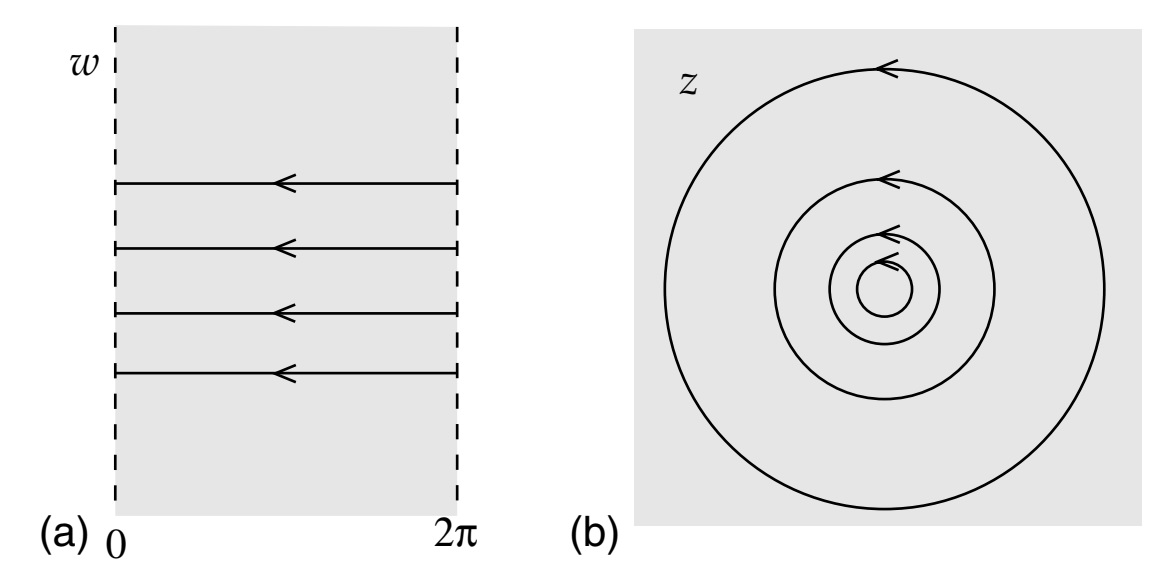
\includegraphics[width=0.8\textwidth]{figure/Fig2.3.jpg}
		\caption{Closed String Coordinates    }
	\end{center}
\end{figure}

In $w$ coordinates, time corresponds to moving $\sigma^{2}=\operatorname{Im} w$. In $z$ coordinates, time moves radially, and the origin is the distant past. These coordinates are related through a conformal transformation.    
For the canonical interpretation of the theory, $w$ coordinates are natural, but $z$ coordinates are also quite useful, and most expressions are written in this frame of reference.    

For holomorphic or anti-holomorphic operators, we can perform a Laurent expansion    
\begin{equation}
	T_{z z}(z)=\sum_{m=-\infty}^{\infty} \frac{L_{m}}{z^{m+2}}, \quad \tilde{T}_{\bar{z} \bar{z}}(\bar{z})=\sum_{m=-\infty}^{\infty} \frac{\tilde{L}_{m}}{\bar{z}^{m+2}} \label{2.6.5}
\end{equation}
The coefficients are called Virasoro generators.    
Given by contour integrals    
\begin{equation}\label{2.6.6}
	L_{m}=\oint_{C} \frac{\dif z}{2 \pi \mi z} \: z^{m+2} T_{z z}(z)
\end{equation}
where $C$ is any contour around the origin counterclockwise.    
At $\sigma^2=0$, the Laurent expansion is an ordinary Fourier transform    
\begin{subequations} \label{2.6.7}
	\begin{align}
		T_{w w}(w)&=-\sum_{m=-\infty}^{\infty} \exp (\mi m \sigma^{1}-m \sigma^{2}) T_{m}   \label{2.6.7a}\\
		T_{\bar{w} \bar{w}}(\bar{w})&=-\sum_{m=-\infty}^{\infty} \exp (-\mi m \sigma^{1}-m \sigma^{2}) \tilde{T}_{m} \label{2.6.7b}
	\end{align}
\end{subequations}
where    
\begin{equation}\label{2.6.8}
	T_{m}=L_{m}-\delta_{m, 0} \frac{c}{24} \:, \qquad \tilde{T}_{m}=\tilde{L}_{m}-\delta_{m, 0} \frac{\tilde{c}}{24} \:.
\end{equation}
The additional offset in $T_0$ comes from the non-tensor transformation (\ref{2.4.26})    
\begin{equation}
	T_{w w}=(\partial_{w} z)^{2} T_{z z}+\frac{c}{24} \:.
\end{equation}
In the $w=\sigma^{1}+\mi \sigma^{2}$ frame, the time-translation Hamiltonian is    
\begin{equation}\label{2.6.10}
	H= \int_{0}^{2 \pi} \frac{\dif \sigma^{1}}{2 \pi} \: T_{22}=L_{0}+\tilde{L}_{0}-\frac{c+\tilde{c}}{24} \:.
\end{equation}
Note the +2 in the Laurent expansion, which is canceled by the conformal transformation of $T$ in the Fourier transform. Similarly, the Laurent expansion of a holomorphic field with weight $h$ will contain $h$ in the exponent.    
Cut open the path integral on a circle where time $Im{w}=\ln |z|$ is constant. The Virasoro generators become operators in the usual sense. Because of holomorphicity, the integral (\ref{2.6.6}) is independent of $C$, so in particular, it is invariant under time translation. That is, they are conserved charges, charges associated with conformal invariance.    

\begin{figure}[!htbp]
	\begin{center}
		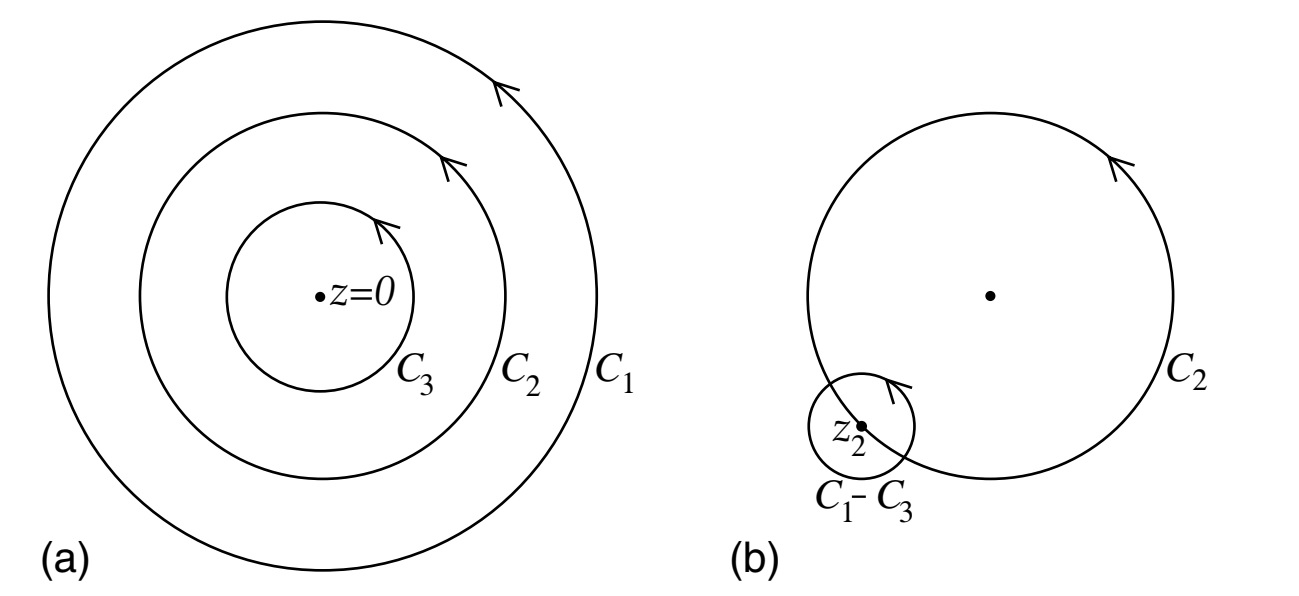
\includegraphics[width=0.6\textwidth]{figure/Fig2.4.jpg}
		\caption{Contours    }\label{Fig2.4}
	\end{center}
\end{figure}
An important fact: the OPE of currents determines the algebra of the corresponding charges.    
Examine general charges $Q_{i}, i=1,2$, given as contour integrals of holomorphic currents    
\begin{equation}
	Q_{i}\{C\}=\oint_{C} \frac{\dif z}{2 \pi \mi} j_{i}\label{2.6.11}
\end{equation}
Examine the combination    
\begin{equation}\label{2.6.12}
	Q_{1}\{C_{1}\} Q_{2}\{C_{2}\}- Q_{2}\{C_{2}\}Q_{1}\{C_{3}\}
\end{equation}
The contour is shown in Figure \ref{Fig2.4}a.    
\begin{figure}[!htbp]
	\begin{center}
		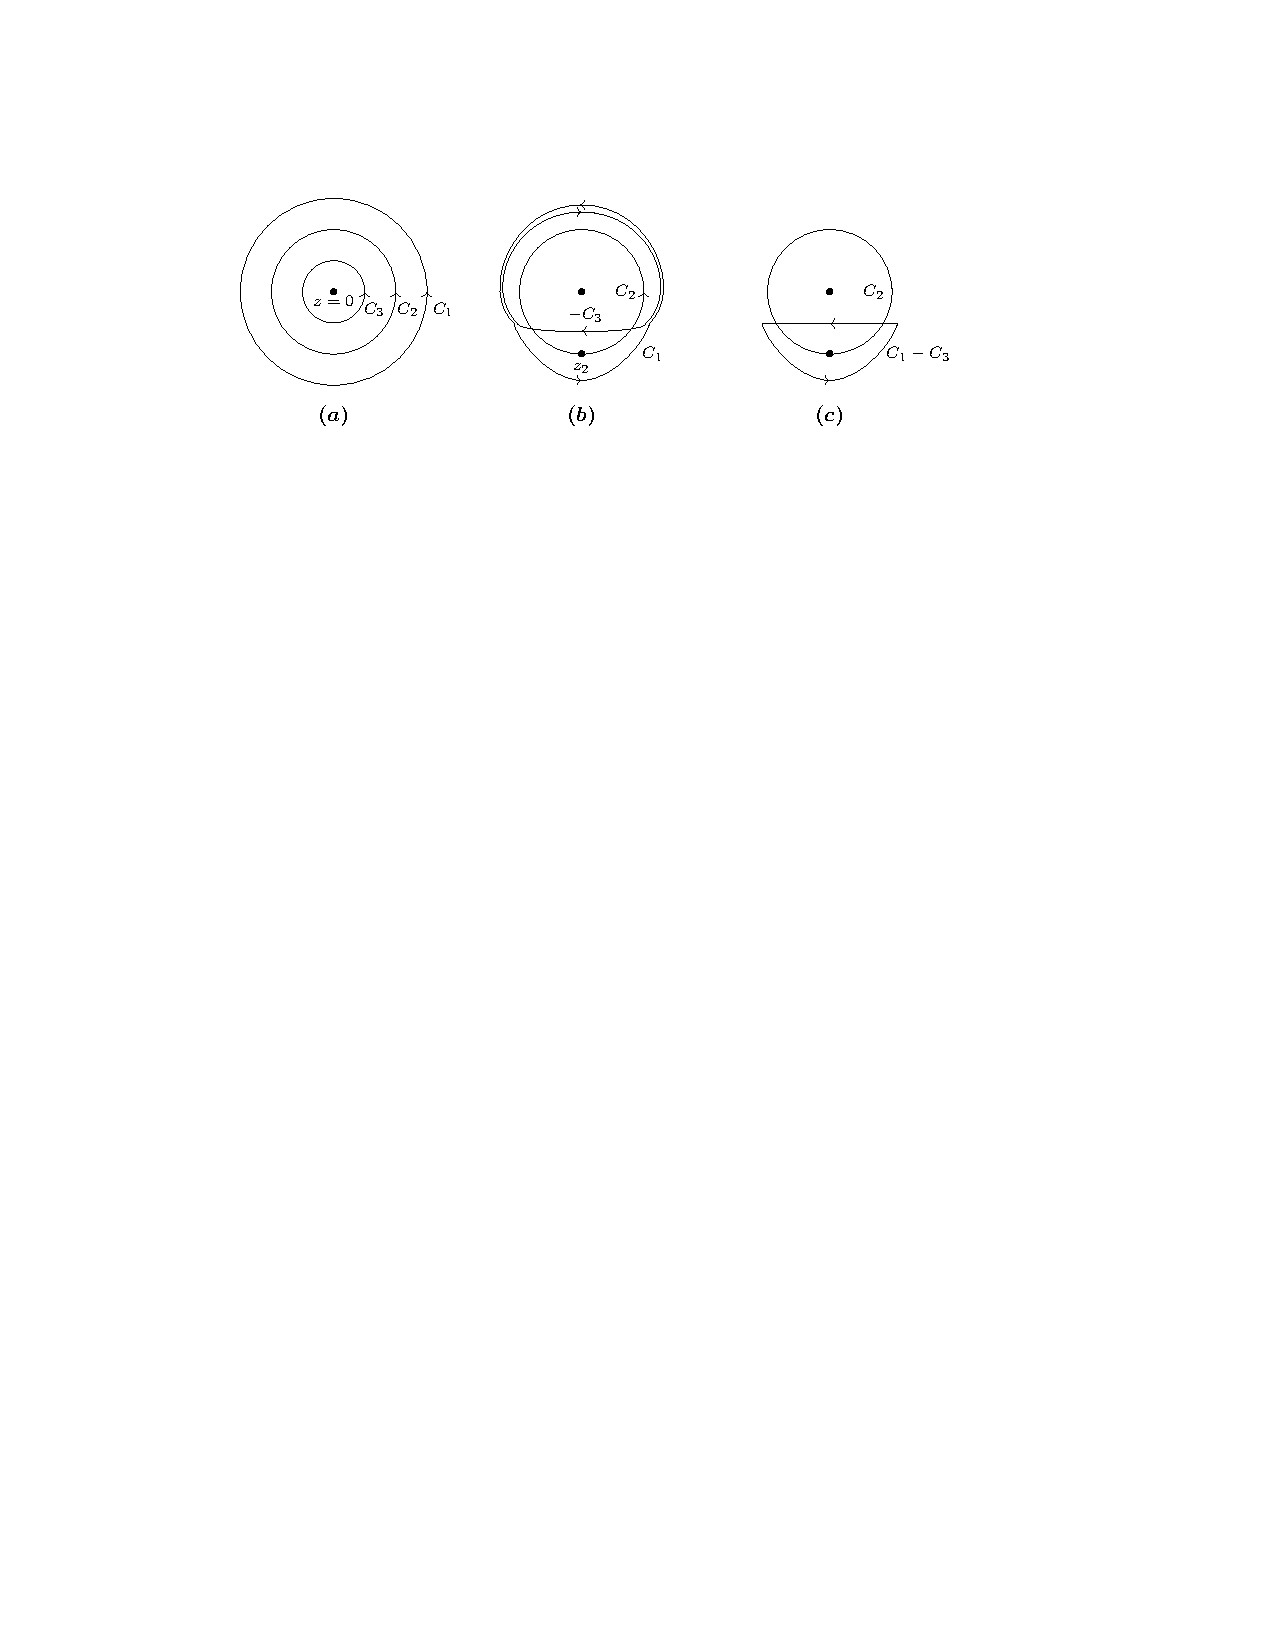
\includegraphics[width=0.8\textwidth]{figure/deforming contour}
		\caption{Deforming Contours. By deforming $C_3$ and $C_1$ is follows that $C_1 - C_3$ is equivalent to a contour around $z_2$.}
		\label{Fig2.4a}
	\end{center}
\end{figure}

The \textbf{order} of factors \textbf{is irrelevant} because they are just integration variables in a path integral (unless the two charges are anti-commuting. In that case there would be an extra sign and all commutators would become anti-commutators).    
When we split the path integral for an operator interpretation, the operator order is determined by time order, here $t_{1}>t_{2}>t_{3}$.    
The path integral for the combination (\ref{2.6.12}) corresponds to the matrix element    
\begin{equation}
	\hat{Q}_{1} \hat{Q}_{2}-\hat{Q}_{2} \hat{Q}_{1} \equiv [\hat{Q}_{1}, \hat{Q}_{2}]
\end{equation}
Now, for a given point $z_2$ on the contour $C_2$, we can deform the difference in contours $C_1, C_3$, as shown in Figure \ref{Fig2.4}b, so the commutator is given by the residue of the OPE    
\begin{equation}
	[Q_{1}, Q_{2}]\{C_{2}\}=\oint_{C_{2}} \frac{\dif z_{2}}{2 \pi \mi} \: \operatorname{Res}_{z_{1} \to z_{2}} j_{1}(z_{1}) j_{2}(z_{2}) \label{2.6.14}
\end{equation}
\begin{tcolorbox}[breakable]
	\begin{proof}
		We start from \eqref{2.6.12} but change the indices of the charges to letters to avoid confusion. It is the radial ordering of the contours that determines the \textbf{ordering} of the corresponding operators, therefore \( Q_a(C_1)Q_b(C_2) - Q_a(C_3)Q_b(C_2) \) object as operators on the Hilbert space is same as \( \hat{Q}_a\hat{Q}_b - \hat{Q}_b\hat{Q}_a = [\hat{Q}_a, \hat{Q}_b] \) as \( C_1 \) is the most outward contour, i.e. the largest time, and \( C_3 \) is the most inward contour, i.e. the smallest time. Now we also have
		\begin{equation}
			Q_a(C_1)Q_b(C_2) - Q_b(C_2)Q_a(C_3) = Q_b(C_2)[Q_a(C_1) - Q_a(C_3)]
			= Q_b(C_2)Q_a(C_1 - C_3)
		\end{equation}
		
		by the contour deformation of fig. \ref{Fig2.4a}. But, on the one hand the transformation of an operator is given by the commutation relation with the corresponding charge, \( \delta Q = [Q, A] \) and on the other hand we have from \eqref{2.3.11} that \( \delta A(z) = \frac{1}{2\pi i} \oint dw \, j(w)A(z) \) with \( j(z) \) the conserved current. Using a transformation under \( Q_a \) on an operator \( Q_b \) for a point on \( C_2 \) and the definition of the charges \eqref{2.6.11} we get
		\begin{align*}
			\delta Q_b\{C_2\} &= [Q_a, Q_b]\{C_2\} = Q_b(C_2)Q_a(C_1 - C_3)\\
			&=\oint_{C_2} \frac{dz_2}{2\pi i} \oint_{C_1-C_3} \frac{dz_1}{2\pi i} \, j_a(z_1)j_b(z_2)
		\end{align*}
		
		But the latter part just picks up the residue of the OPE \( j_a(z_1)j_b(z_2) \) when \( z_1 \to z_2 \). Thus
		
		\begin{equation}
			\delta Q_b\{C_2\} = \oint_{C_2} \frac{dz_2}{2\pi i} \, \operatorname{Res}_{z_1 \to z_2} j_a(z_1)j_b(z_2)
		\end{equation}
		
		and so we find
		
		\begin{equation}
			[\hat{Q}_a, \hat{Q}_b] = \oint_{C_2} \frac{dz_2}{2\pi i} \, \operatorname{Res}_{z_1 \to z_2} j_a(z_1)j_b(z_2)
		\end{equation}
		
		Which is the relation that allows us to pass from OPEs to the commutation relations of conserved charges.
	\end{proof}
\end{tcolorbox}
\begin{tcolorbox}[breakable]
	\begin{remark}
		The essential content of current--current OPEs is that charge commutators are determined by residues. If
		\begin{equation}
			J^a(z)\,J^b(w) \sim \frac{f^{ab}{}_c\, J^c(w)}{z-w} + \cdots,
		\end{equation}
		then defining
		\begin{equation}
			Q^a = \frac{1}{2\pi i}\oint dz\, J^a(z),
		\end{equation}
		we obtain
		\begin{equation}
			[Q^a, Q^b] = f^{ab}{}_c\, Q^c.
		\end{equation}
		Thus, the Lie algebra of charges is encoded in the simple pole of the current OPE.
	\end{remark}
\end{tcolorbox}
Contour discussion allows us to pass back and forth between OPEs and commutation relations.    
Let us emphasize that for conserved currents, knowing the singularity in the OPE is equivalent to knowing the corresponding charge commutator algebra. Replacing the conserved charge $Q_{2}\left\{C_{2}\right\}$ with an arbitrary operator, the same discussion applies:    
\begin{equation}
	[Q, \mathscr{A}(z_{2}, \bar{z}_{2})]=\operatorname{Res}_{z_{1} \to z_{2}} j(z_{1}) \mathscr{A}(z_{2}, \bar{z}_{2})
	=\frac{1}{\mi \epsilon} \delta \mathscr{A}(z_{2}, \bar{z}_{2}) \label{2.6.15}
\end{equation}
This is exactly the familiar statement: charge $Q$ generates the corresponding transformation. 
\begin{tcolorbox}[breakable]
\begin{remark}
	The symmetry action of $Q$ is encoded in the simple pole of the current--operator OPE:
	\begin{equation}
		j(z)\,\mathscr A(w,\bar w)
		\sim \frac{X(w,\bar w)}{z-w} + \cdots
		\;\Longrightarrow\;
		[Q,\mathscr A(w,\bar w)] = X(w,\bar w),
	\end{equation}
	with $\delta \mathscr A = i\epsilon\, X$. Placing the operator at the origin and using the state--operator correspondence
	\begin{equation}
		\mathscr A(0)\;\leftrightarrow\;|\mathscr A\rangle,
	\end{equation}
	this becomes
	\begin{equation}
		Q\,|\mathscr A\rangle = |X\rangle.
	\end{equation}
	Thus, the residue of the OPE determines both the transformation of operators and the action of the charge on states.
\end{remark}
\end{tcolorbox}   
Similarly, for contour integrals of anti-holomorphic currents    
\begin{equation}
	\tilde{Q}\{C\}=-\oint_{C} \frac{\dif \bar{z}}{2 \pi \mi} \: \tilde{\jmath} \:, \label{2.6.16}
\end{equation}
Ward identity and contour discussion imply    
\begin{equation}
	[\tilde{Q}, \mathscr{A}(z_{2}, \bar{z}_{2})]=\operatorname{Res}_{\bar{z}_{1} \to \bar{z}_{2}} \tilde{\jmath}(\bar{z}_{1}) 
	\mathscr{A}(z_{2}, \bar{z}_{2})=\frac{1}{\mi \epsilon} \delta \mathscr{A}(z_{2}, \bar{z}_{2}) \label{2.6.17}
\end{equation}
Applied to the Virasoro algebra (\ref{2.6.6}),    
\begin{align}
	&\operatorname{Res}_{z_{1} \to z_{2}} z_{1}^{m+1} T(z_{1}) z_{2}^{n+1} T(z_{2})  \nonumber \\
	&\quad =\operatorname{Res}_{z_{1} \rightarrow z_{2}} z_{1}^{m+1} z_{2}^{n+1}\Biggl(\frac{c}{2 z_{12}^{4}}+\frac{2}{z_{12}^{2}} T(z_{2})
	+\frac{1}{z_{12}} \partial T(z_{2})\Biggr) \nonumber \\
	&\quad =\frac{c}{12}(\partial^{3} z_{2}^{m+1}) z_{2}^{n+1}+2(\partial z_{2}^{m+1}) z_{2}^{n+1} T(z_{2})
	+z_{2}^{m+n+2} \partial T(z_{2}) \nonumber \\
	&\quad =\frac{c}{12}(m^{3}-m) z_{2}^{m+n-1}+(m-n) z_{2}^{m+n+1} T(z_{2})+\text {total derivative}  \label{2.6.18}
\end{align}
where $j_{m}(z)=z^{m+1} T(z)$.    
Then the $z_2$ contour integral on the right gives the Virasoro algebra:    
\begin{equation}\label{2.6.19}
	\left[L_{m}, L_{n}\right]=(m-n) L_{m+n}+\frac{c}{12}\left(m^{3}-m\right) \delta_{m,-n}
\end{equation}
$\tilde{L}_{m}$ satisfies the same algebra with central charge $\tilde{c}$.    
Thus any CFT has infinitely many conserved charges, i.e., Virasoro generators. They act in Hilbert space and satisfy algebra (\ref{2.6.19}). Focus on a few simple properties first. Generally, dealing with eigenstates of $L_{0}$ and $\tilde{L}_{0}$, generator $L_{0}$ satisfies    
\begin{equation}
	\left[L_{0}, L_{n}\right]=-n L_{n}
\end{equation}
If $|\psi\rangle$ is an eigenstate of $L_{0}$ with eigenvalue $h$, then    
\begin{equation}
	L_{0} L_{n}|\psi\rangle=L_{n}\left(L_{0}-n\right)|\psi\rangle=(h-n) L_{n}|\psi\rangle
\end{equation}
So $L_n|\psi\rangle$ is an eigenstate with eigenvalue $h-n$. Generators with $n<0$ raise the eigenvalue of $L_{0}$, while $n>0$ lowers it.    
Three generators $L_{0}$ , $L_{\pm 1}$ form a closed algebra without central charge:    
\begin{equation}
	\left[L_{0}, L_{1}\right]=-L_{1}, \quad\left[L_{0}, L_{-1}\right]=L_{-1}, \quad\left[L_{1}, L_{-1}\right]=2 L_{0}
\end{equation}
This is the algebra $SL(2,\mathbb{R})$, which differs from $SU(2)$ by a sign. For a holomorphic tensor field $\mathcal{O}$ with weight $(h,0)$, the Laurent coefficients are    
\begin{equation}
	\mathcal{O}(z)=\sum_{m=-\infty}^{\infty} \frac{_m}{z^{m+h}} \label{2.6.23}
\end{equation}
From OPE (\ref{2.4.16}) the commutator is obtained    
\begin{equation}
	[L_{m}, \mathcal{O}_{n}]=[(h-1) m-n] \mathcal{O}_{m+n} \:.
	\label{2.6.24}
\end{equation}
Again, $n>0$ mode lowers $L_0$, $n<0$ mode raises $L_0$.    

\begin{tcolorbox}[breakable]
	\begin{proof}
		Proof of (\ref{2.6.24}): in (\ref{2.6.17}) let $j_{m}(z)=z^{m+1} T(z)$ and $j_{n}(z)=z^{n+h-1} \mathcal{O}(z)$, then    
		\begin{align*}
			&\quad \operatorname{Res}_{z_1 \rightarrow z_2}  z_1^{m+1} T(z_{1}) z_2^{n+h-1} \mathcal{O}(z_{2})\\
			&=\operatorname{Res}_{z_1 \rightarrow z_2} z_1^{m+1} z_2^{n+h-1}\left(\frac{h}{z_{12}^2} O(z_2)+\frac{1}{z_{12}} \partial \mathcal{O}(z_2)\right)\\
			&=h(\partial z_2^{m+1})z_2^{n+h-1}\mathcal{O}(z_2)+z_2^{m+n+h}\partial\mathcal{O}(z_2)\\
			&=h(m+1)z_2^{m+n+h-1}\mathcal{O}(z_2)-(m+n+h)z_2^{m+n+h-1}\mathcal{O}(z_2)+ \text{total derivative}
		\end{align*}
		Using (\ref{2.6.23}), the first term becomes    
		$$h(m+1)z_2^{m+n+h-1}\mathcal{O}(z_2) \sim h(m+1) \sum \mathcal{O}_q z_2^{m+n-q-1} \sim h(m+1)\mathcal{O}_{m+n}$$
		The second term becomes    
		\begin{align*}
			-(m+n+h) z_{2}^{m+n+h-1} \sum \frac{\mathcal{O}_{q}}{z_{2}^{q+h}} \sim-(m+n+h) \mathcal{O}_{m+n}
		\end{align*}
		Adding the two yields (\ref{2.6.24}).    
	\end{proof}
\end{tcolorbox}

For open strings, let    
\begin{equation}
	0 \leq \operatorname{Re} w \leq \pi \quad \Leftrightarrow \quad \operatorname{Im} z \geq 0
\end{equation}
where $z=-\exp (-\mi w)$. 
The coordinate region is shown in Figure \ref{Fig2.5}.    
\begin{figure}[!htbp]
	\begin{center}
		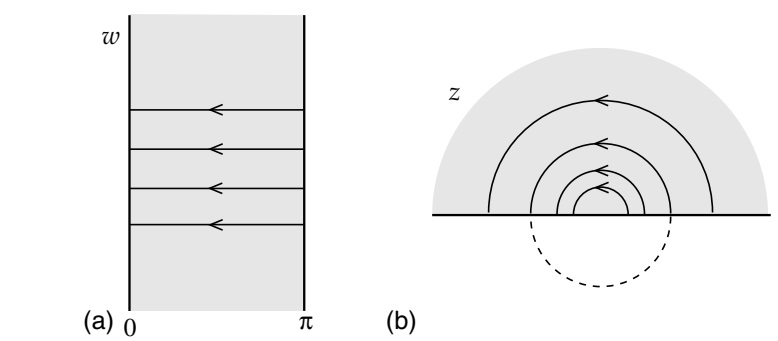
\includegraphics[width=0.8\textwidth]{figure/Fig2.5.jpg}
		\caption{Contours    }\label{Fig2.5}
	\end{center}
\end{figure}


\noindent At the boundary, energy-momentum satisfies    
\begin{equation}\label{2.6.26}
	T_{a b} n^{a} t^{b}=0 \:,
\end{equation}
where $n^{a}$ and $t^{b}$ are the normal vector and tangential vector respectively. To see this, examine a coordinate system where the boundary is a straight line. The appearance of the boundary breaks the normal translation invariance, but not the tangential one, making the current $T_{a b} t^{b}$ still conserved. Then the boundary condition (\ref{2.6.26}) is a statement that the current out of the boundary is zero.    
In the current case, this becomes    
\begin{equation}
	T_{w w}=T_{\bar{w} \bar{w}}, \: \operatorname{Re} w=0 \:, \pi \qquad \Leftrightarrow \quad T_{z z}=T_{\bar{z} \bar{z}}\:, \operatorname{Im} z=0 \:.
\end{equation}
It is convenient to use the "doubling trick".    
Define $T_{zz}$ in the lower half $z$-plane as the value of $T_{\bar{z} \bar{z}}$ at the image point $z^{\prime}=\bar{z}$ in the upper half plane:    
\begin{equation}
	T_{z z}(z) \equiv T_{\bar{z} \bar{z}}\left(\bar{z}^{\prime}\right), \quad \operatorname{Im} z<0 \:.
\end{equation}
Equations of motion and boundary conditions are summarized as: $T_{z z}$ is holomorphic throughout the complex plane.    
Because the boundary condition couples $T$ and $\tilde{T}$, there is only one set of Virasoro algebra:    
\begin{align}
	L_{m} &=\frac{1}{2 \pi \mi} \int_{C}\Bigl(\dif z \:z^{m+1} T_{z z}-\dif \bar{z} \: \bar{z}^{m+1} T_{\bar{z} \bar{z}}\Bigr) \nonumber  
	&=\frac{1}{2 \pi \mi} \oint \dif z\: z^{m+1} T_{z z}(z)
\end{align}
In the first line, the contour is a semicircle centered at the origin; in the second line, we use the "doubling trick" to write $L_m$ as a closed contour.    
Once again, these $L_{m}$ satisfy the Virasoro algebra    
\begin{equation}
	\left[L_{m}, L_{n}\right]=(m-n) L_{m+n}+\frac{c}{12}\left(m^{3}-m\right) \delta_{m,-n} \:.
\end{equation}

\section{\texorpdfstring{Mode expansions}{2.7 Mode expansions}} \label{sec:2.7}

\subsection*{Free Scalar}
In free field theory, the field decomposes into harmonic oscillators, and the spectrum and energy-momentum tensor can be given in mode form. We start with closed strings.    
In the theory of $X^\mu$, $\partial X$ and $\bar{\partial} X$ are anti-holomorphic. So there is a similar Laurent expansion:    
\begin{equation}\label{2.7.1}
	\partial X^{\mu}(z)=-\mi\biggl(\frac{\alpha^{\prime}}{2}\biggr)^{1 / 2} \sum_{m=-\infty}^{\infty} \frac{\alpha_{m}^{\mu}}{z^{m+1}}\:, \qquad 
	\bar{\partial} X^{\mu}(\bar{z})=-\mi\biggl(\frac{\alpha^{\prime}}{2}\biggr)^{1 / 2} \sum_{m=-\infty}^{\infty} \frac{\tilde{\alpha}_{m}^{\mu}}{\bar{z}^{m+1}} \:.
\end{equation}
Equivalently,    
\begin{subequations}\label{2.7.2}
	\begin{align}
		\alpha_{m}^{\mu}&=\biggl(\frac{2}{\alpha^{\prime}}\biggr)^{1 / 2} \oint \frac{\dif z}{2 \pi}\: z^{m} \partial X^{\mu}(z) \:, \label{2.7.2a} \\
		\tilde{\alpha}_{m}^{\mu}&=-\biggl(\frac{2}{\alpha^{\prime}}\biggr)^{1 / 2} \oint \frac{\dif \bar{z}}{2 \pi} \: \bar{z}^{m} \bar{\partial} X^{\mu}(\bar{z}) \:.
		\label{2.7.2b}
	\end{align}
\end{subequations}
The single-valuedness of $X^\mu$ implies $\alpha_{0}^{\mu}=\tilde{\alpha}_{0}^{\mu}$, furthermore, the Noether current of spacetime translation is $\mi \partial_{a} X^{\mu} / \alpha^{\prime}$, so spacetime momentum    
\begin{equation}\label{2.7.3}
	p^{\mu}=\frac{1}{2 \pi \mi} \oint_{C} (\dif z \: j^{\mu}-\dif \bar{z}\: \tilde{\jmath}^{\mu})
	=\biggl(\frac{2}{\alpha^{\prime}}\biggr)^{1 / 2} \alpha_{0}^{\mu}=\biggl(\frac{2}{\alpha^{\prime}}\biggr)^{1 / 2} \tilde{\alpha}_{0}^{\mu}
\end{equation}
Integrating expression (\ref{2.7.1}) gives    
\begin{equation}\label{2.7.4}
	X^{\mu}(z, \bar{z})=x^{\mu}- \mi \frac{\alpha^{\prime}}{2} p^{\mu} \ln |z|^{2}+\mi\left(\frac{\alpha^{\prime}}{2}\right)^{1 / 2} \sum_{m=-\infty \atop m \neq 0}^{\infty} \frac{1}{m}\left(\frac{\alpha_{m}^{\mu}}{z^{m}}+\frac{\tilde{\alpha}_{m}^{\mu}}{\bar{z}^{m}}\right) \:.
\end{equation}
Since $|z|>0$, the logarithm in mode decomposition does not have any branch cut. Whether starting from standard canonical commutators, or from contour discussions or the $XX$ OPE, one can give    
\begin{subequations} \label{2.7.5}
	\begin{align}
		[\alpha_{m}^{\mu}, \alpha_{n}^{\nu}] &= [\tilde{\alpha}_{m}^{\mu}, \tilde{\alpha}_{n}^{\nu}]=m \delta_{m,-n} \eta^{\mu \nu} \:, \label{2.7.5a} \\
		[x^{\mu}, p^{\nu}] &= \mi \eta^{\mu \nu} \:, \label{2.7.5b}  
	\end{align}
\end{subequations}
Other commutators are zero.    
The spectrum starts from the state $\lvert 0 ; k\rangle$ with momentum $k^\mu$, which is annihilated by all $n>0$ lowering modes $\alpha_n^\mu$, while other states in the spectrum are given by the action of raising modes $(n<0)$ in all possible ways on $\lvert 0 ; k\rangle$.    

We now wish to expand Virasoro generators in mode operator form.    
Substituting the Laurent expansion of $X^\mu$ into the energy-momentum tensor (\ref{2.4.4}) and collecting terms of a given order in $z$, gives    
\begin{equation}\label{2.7.6}
	L_{m} \sim \frac{1}{2} \sum_{n=-\infty}^{\infty} \alpha_{m-n}^{\mu} \alpha_{\mu n} \:.
\end{equation}
"$\sim$" means neglecting the order of operators. When $m\neq 0$, the expansion (\ref{2.7.6}) is well-defined and correct—the mode operator in each term commutes so the sequence is not important.    
For $m=0$, place the lowering operators on the right and introduce a normal-ordering constant:    
\begin{equation}
	L_{0}=\frac{\alpha^{\prime} p^{2}}{4}+\sum_{n=1}^{\infty}\left(\alpha_{-n}^{\mu} \alpha_{\mu n}\right)+a^{X} \:. \label{2.7.7}
\end{equation}
We encountered the same problem in Section 1.3, where we dealt with it in a heuristic way. Now there is a finite and explicit definition on the left, defined by Laurent coefficients in the $\mathrel{:\::}$ ordered energy-momentum tensor, so the normal-ordering constant is finite and calculable. There are several ways to determine it, the simplest is using the Virasoro algebra,    
\begin{equation}\label{2.7.8}
	2 L_{0}|0 ;
	0\rangle=(L_{1} L_{-1}-L_{-1} L_{1})|0 ; 0\rangle=0  \:,
\end{equation}
thus    
\begin{equation}
	a^{X}=0 \:. \label{2.7.9}
\end{equation}
Here we have used the known forms of $L_1, L_{-1}$: each term either contains a lowering operator or $p^\mu$, thus annihilating $|0 ; 0\rangle$.    
From the OPE, we determined the central charge of the Virasoro algebra. It can also be directly derived from the mode operator expression of the Virasoro algebra.    

Introduce a new notation. Symbol $ \mathrel{: \: :}$ represents creation-annihilation normal ordering: place all lowering operators on the right of all creation operators. Note there is a negative sign when exchanging anti-commuting operators.    
For this reason, we include $p^\mu$ among the lowering operators and $x^\mu$ among the raising operators.    
In this notation, we can write    
\begin{equation}\label{2.7.10}
	L_{m}=\frac{1}{2} \sum_{n=-\infty}^{\infty}\mathrel{ : \alpha_{m-n}^{\mu} \alpha_{\mu n} : }
\end{equation}


We have now introduced two forms of normal ordering, namely conformal normal ordering $\mathrel{:\::}$ and creation-annihilation normal ordering $\mathrel{: \: :}$. The advantage of the former is that the operators it produces have simpler OPEs and conformal transformation properties; the latter may be more familiar to readers, and it is more convenient for dealing with matrix elements of operators. We now present the relationship between the two. Start by comparing time-ordered products and creation-annihilation normal products.    
For the product $X^{\mu}(z, \bar{z}) X^{\nu}(z^{\prime}, \bar{z}^{\prime})$ with $\lvert z \rvert >\lvert z^{\prime}\rvert$, substitute in the mode expansion and move the lowering operator in $X^{\mu}(z, \bar{z})$ to the right:    
\begin{align}
	X^{\mu}(z, \bar{z}) X^{\nu}(z^{\prime}, \bar{z}^{\prime}) &= \mathrel{ : X^{\mu}(z, \bar{z}) X^{\nu}(z^{\prime}, \bar{z}^{\prime}) : }  +\frac{\alpha^{\prime}}{2} \eta^{\mu \nu}\left[-\ln |z|^{2}+\sum_{m=1}^{\infty} \frac{1}{m}\left(\frac{z^{\prime m}}{z^{m}}+\frac{\bar{z}^{\prime m}}{\bar{z}^{m}}\right)\right] \nonumber \\
	&=\mathrel{ : X^{\mu}(z, \bar{z}) X^{\nu}(z^{\prime}, \bar{z}^{\prime}) : }-\frac{\alpha^{\prime}}{2} \eta^{\mu \nu}\ln \lvert z-z^\prime\rvert^{2} \label{2.7.11}
\end{align}
Since $|z|>\lvert z^{\prime}\rvert$, the left side is time-ordered and the sum converges.    
Define the relationship between the time-ordered product and the conformal normal product given by (\ref{2.1.21}) (definition (\ref{2.1.21}) uses path integral language, so the products on the right are time-ordered under the operator system). This is the same as (\ref{2.7.11}), making    
\begin{equation}\label{2.7.12}
	\mathrel{ : X^{\mu}(z, \bar{z}) X^{\nu}(z^{\prime}, \bar{z}^{\prime}) : } = \mathrel{: X^{\mu}(z, \bar{z}) X^{\nu}(z^{\prime}, \bar{z}^{\prime})}:
\end{equation}
This relationship does not hold in a general CFT, and in fact, some combination of $p^\mu$ and lowering operators gives a simpler result. This also does not hold for the $w$ form of conformal normal sequence of operators.    
From (\ref{2.7.12}) the mode expansion (\ref{2.7.10}) can be written immediately, and the second derivation of $a^{X}=0$ is given.    

The creation-annihilation normal product of more than two $X^\mu$ has the same combinatorial factors as the $\mathrel{:\::}$ ordering. That is, they are both obtained from time-ordered products by summing over all contractions—Wick's theorem in field theory.    
To convert the normal ordering of an operator from one form to another, use the difference of two-point functions for contractions and sum over them. That is, if we have two orderings,    
\begin{equation}
	[X^{\mu}(z, \bar{z}) X^{v}(z^{\prime}, \bar{z}^{\prime})]_{1} = [X^{\mu}(z, \bar{z}) X^{v}(z^{\prime}, \bar{z}^{\prime})]_{2} 
	+\eta^{\mu v} \Delta (z, \bar{z}, z^{\prime}, \bar{z}^{\prime}) \:, \label{2.7.13}
\end{equation}
then for a general operator $\mathscr{F}$    
\begin{equation}
	[\mathscr{F}]_{1}=\exp \left(\frac{1}{2} \int \dif^{2} z\, \dif^{2} z^{\prime}\: \Delta(z, \bar{z}, z^{\prime}, \bar{z}^{\prime}) \frac{\delta}{\delta X^{\mu}(z, \bar{z})} \frac{\delta}{\delta X_{\mu}(z^{\prime}, \bar{z}^{\prime})}\right)[\mathscr{F}]_{2} \:.
	\label{2.7.14}
\end{equation}

For a linear dilaton CFT, the Laurent expansion and commutator are invariant, while the Virasoro generator contains an extra term    
\begin{equation}
	L_{m}=\frac{1}{2} \sum_{n=-\infty}^{\infty} \mathrel{ : \alpha_{m-n}^{\mu} \alpha_{\mu n} : } + \:\mi\left(\frac{\alpha^{\prime}}{2}\right)^{1 / 2}(m+1) V^{\mu} \alpha_{\mu m} \:.
\end{equation}

\subsection*{ $bc$ CFT}

Fields $b$ and $c$ have Laurent expansion    
\begin{equation} \label{2.7.16}
	b(z)=\sum_{m=-\infty}^{\infty} \frac{b_{m}}{z^{m+\lambda}}\:, \qquad c(z)=\sum_{m=-\infty}^{\infty} \frac{c_{m}}{z^{m+1-\lambda}} \:.
\end{equation}
Precisely, if $\lambda$ is an integer, they are just Laurent expansions. The half-integer case is also interesting, and we will deal with it carefully in Chapter 10. The OPE gives the anti-commutator    
\begin{equation}
	\left\{b_{m}, c_{n}\right\}=\delta_{m,-n} \:.
	\label{2.7.17}
\end{equation}
These operators anti-commute with other grassmann numbers as well. First examine states annihilated by all $n>0$ operators. The oscillator algebra of $b_0$ and $c_0$ generates two such ground states $\lvert\downarrow\rangle$ and $\lvert\uparrow\rangle$. They have properties    
\begin{subequations} \label{2.7.18}
	\begin{align}
		b_{0}\lvert\downarrow\rangle &=0\:, \quad b_{0} \lvert \uparrow\rangle=\lvert\downarrow\rangle \:, \label{2.7.18a} \\
		c_{0}\lvert\downarrow\rangle &=\lvert\uparrow\rangle \:, \quad c_{0}\lvert\uparrow\rangle=0 \:, \label{2.7.18b} \\
		b_{n}\lvert\downarrow\rangle &=b_{n}\lvert\uparrow\rangle=c_{n}\lvert \downarrow\rangle=c_{n}\lvert\uparrow\rangle=0 \:, \quad n>0  \:.
		\label{2.7.18c}
	\end{align}
\end{subequations}
Ordinary states are obtained by acting on these states with $n<0$ modes, but due to anti-commutation, they can act at most once. For some later reasons, it will be convenient to group $b_0$ with lowering operators and $c_0$ with raising operators, so we pick $\lvert \downarrow\rangle$ as the ghost vacuum $|0\rangle$. In string theory we will have a holomorphic $bc$ theory and an anti-holomorphic $\tilde{b} \tilde{c}$ theory. Each has $\lambda=2$.     
And the closed string spectrum contains the product of two pairs of theories.    
The Virasoro generators are    
\begin{equation}
	L_{m}=\sum_{n=-\infty}^{\infty}(m \lambda-n) \mathrel{ : b_{n} c_{m-n} : }+ \:\delta_{m, 0} a^{\mathrm{g}} \:.
	\label{2.7.19}
\end{equation}
The ordering constant can be determined like (\ref{2.7.8}), which gives    
\begin{align}
	2 L_{0}\lvert \downarrow\rangle &= (L_{1} L_{-1}-L_{-1} L_{1}) \lvert \downarrow\rangle \nonumber \\
	&= (\lambda b_{0} c_{1})[(1-\lambda) b_{-1} c_{0}]\lvert \downarrow\rangle=\lambda(1-\lambda)\lvert \downarrow\rangle \:.
	\label{2.7.20}
\end{align}
Thus $a^{\mathrm{g}}=\frac{1}{2} \lambda(1-\lambda)$ and    
\begin{equation}
	L_{m}=\sum_{n=-\infty}^{\infty}(m \lambda-n) \mathrel{ : b_{n} c_{m-n} : } + \: \frac{\lambda(1-\lambda)}{2} \delta_{m, 0} \:.
	\label{2.7.21}
\end{equation}
The constant can also be obtained by solving for the relationship between $\mathrel{:\::}$ and $\mathrel{: \: :}$.    
For the ghost number current (\ref{2.5.14}), $j={-}:\mathrel{bc}:$, the charge is    
\begin{align}
	N^{\mathrm{g}} &=-\frac{1}{2 \pi \mi} \int_{0}^{2 \pi} \dif w \: j_{w} \nonumber \\
	&=\sum_{n=1}^{\infty}(c_{-n} b_{n}-b_{-n} c_{n})+c_{0} b_{0}-\frac{1}{2} \:.
	\label{2.7.22}
\end{align}
It satisfies    
\begin{equation}
	[N^{\mathrm{g}}, b_{m}]=-b_{m}\:, \qquad  [N^{\mathrm{g}}, c_{m}]=c_{m} \:, \label{2.7.23}
\end{equation}
thus $c$ minus $b$ number is excitation. The ground states have ghost number $\pm \frac{1}{2}$:    
\begin{equation}
	N^{\mathrm{g}}\lvert \downarrow\rangle = -\frac{1}{2}\lvert \downarrow\rangle \:, \qquad 
	N^{\mathrm{g}}\lvert \uparrow\rangle = \frac{1}{2}\lvert \uparrow\rangle \:.
	\label{2.7.24}
\end{equation}
This depends on the value of the ordering constant, but can be guessed: the average ghost number of the ground state should be zero and the ghost number changes sign under $b \leftrightarrow c$.    

\subsection*{ Open String}
For open strings, Neumann boundary condition becomes $\partial_z X^{\mu}=\partial_{\bar{z}} X^{\mu}$ on the real axis.    
There is only one set of modes, the boundary condition requires $\alpha_{m}^{\mu}=\tilde{\alpha}_{m}^{\mu}$ in the expansion (\ref{2.7.1}).    
The spacetime momentum integral (\ref{2.7.3}) only integrates a semicircle, so the current normalization is    
\begin{equation}
	\alpha_{0}^{\mu}= (2 \alpha^{\prime})^{1 / 2} p^{\mu} \:. \label{2.7.25}
\end{equation}
Then the expansion for $X^\mu$ is    
\begin{equation}
	X^{\mu}(z, \bar{z})=x^{\mu}- \mi \alpha^{\prime} p^{\mu} \ln |z|^{2} + \mi\left(\frac{\alpha^{\prime}}{2}\right)^{1 / 2} 
	\sum_{m=-\infty \atop m \neq 0}^{\infty} \frac{\alpha_{m}^{\mu}}{m} (z^{-m}+\bar{z}^{-m}) \:.
	\label{2.7.26}
\end{equation}
Also    
\begin{equation}
	L_{0}=\alpha^{\prime} p^{2}+\sum_{n=1}^{\infty} \alpha_{-n}^{\mu}\cdot \alpha_{\mu n} \:. \label{2.7.27}
\end{equation}
Commutators as usual    
\begin{equation}
	[\alpha_{m}^{\mu}, \alpha_{n}^{\nu}]=m \delta_{m,-n} \eta^{\mu \nu} \: , \qquad [x^{\mu}, p^{\nu}]= \mi \eta^{\mu \nu} \:.
	\label{2.7.28}
\end{equation}

For $bc$ theory, the boundary conditions related to strings are    
\begin{equation}
	c(z)=\tilde{c}(\bar{z})\: , \quad b(z)=\tilde{b}(\bar{z}) \:, \quad \operatorname{Im} z=0 \:,  \label{2.7.29}
\end{equation}
which is the $z$ coordinate form where the boundary is on the real axis.    
Then we can use the doubling trick to write the holomorphic and anti-holomorphic fields in the upper half plane in the form of holomorphic fields in the entire plane    
\begin{equation}
	c(z) \equiv \tilde{c}(\bar{z}^{\prime})\:, \quad b(z) \equiv \tilde{b}(\bar{z}^{\prime})\:, \quad \operatorname{Im}(z) \leq 0\,,\: z^{\prime}=\bar{ z} \:.  \label{2.7.30}
\end{equation}
So for open strings, each $b$ and $c$ has a set of Laurent expansions.    
\section{\texorpdfstring{Vertex operators}{2.8 Vertex operators}}

In quantum field theory, on one hand, there is the state space of the theory; on the other hand, there is the set of local operators. In conformal field theory, there is a simple and useful isomorphism between them when quantizing the CFT on a circle.
Examine the semi-infinite cylinder in $w$-coordinates,    
\begin{equation}
	0 \leq \operatorname{Re} w \leq 2 \pi \:, \quad w \sim w+2 \pi \:, \quad \operatorname{Im} w \leq 0 \:, \label{2.8.1}
\end{equation}
under $z=\exp (-\mi w)$, this semi-infinite cylinder is mapped to a unit disk.    
As shown in Figure \ref{Fig2.6}.  Under this transformation, the entire $\sigma_2=-\infty$ hypersurface is mapped to the single point $z=0$. This naturally raises the question of whether any information has been lost. At first glance, it appears that the entire Hilbert space of the CFT is localized at a point in this coordinate system. If so, what structure encodes the seemingly lost information?

In a general QFT, this mapping is in fact singular: the metric $ds^2_{\rm cyl}$ becomes ill-defined at the origin, so one cannot meaningfully compress an entire hypersurface to a point. However, in a CFT, dilatation symmetry saves the situation. Since the states we consider form a basis of eigenstates of the dilatation operator, one can shrink any sphere to a point without losing information.

There is also a conceptual shift in locality. Operators defined on the $\sigma_2=-\infty$ hypersurface are intrinsically non-local objects from the radial point of view, whereas operators inserted at $z=0$ are genuine local operators. The information of the Hilbert space is therefore not lost, but reorganized and encoded in the space of local operator insertions at the origin, via the state--operator correspondence.
\begin{figure}[!htbp]
	\begin{center}
		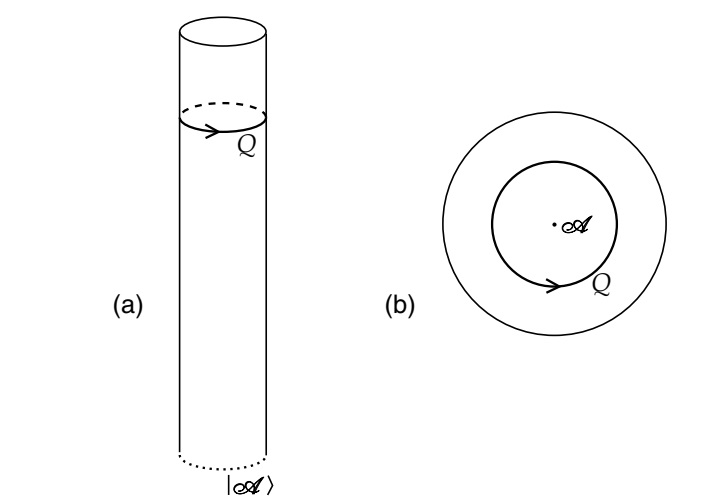
\includegraphics[width=0.8\textwidth]{figure/Fig2.6.jpg}
		\caption{(a) Semi-infinite cylinder in $w$-coordinates, with initial state $\lvert\mathscr{A}\rangle$ and charge $Q$. 
			(b) Conformal equivalent unit disk, with local operator $\mathscr{A}$ and contour integral of $Q$.    }\label{Fig2.6}
	\end{center}
\end{figure}

For free field theory, it is easy to get the detailed form of this isomorphism. Suppose there is a conserved charge $Q$ acting on state $\lvert\mathscr{A}\rangle$ as in Figure \ref{Fig2.6}(a). By using the OPE to calculate the contour integral in Figure \ref{Fig2.6}(b), the corresponding local operator can be found. Corresponding to the identity operator, we equate the state $|1\rangle$.    
When there is no operator at the origin, $\partial X^{\mu}$ and $\bar{\partial} X^{\mu}$ are holomorphic and anti-holomorphic inside the contour of $Q$ in Figure \ref{Fig2.6}(b). Define the contour integral (\ref{2.7.2}) of $\alpha_{m}^{\mu}$ and $\tilde{\alpha}_{m}^{\mu}$ for $m \geq 0$ to have no pole, thus yielding zero.    
$\lvert 1\rangle$ is annihilated by these modes, indicating it is the ground state,    
\begin{equation}
	\lvert 1\rangle=\lvert 0 ; 0\rangle \:, \label{2.8.2}
\end{equation}
now examine, for example, the state $\alpha_{-m}^{\mu}|1\rangle$ for positive $m$.    
Transitioning to Figure \ref{Fig2.6}(b), $Q=\alpha_{-m}^{\mu}$, the field is holomorphic within the contour, thus for $m\geq 1$ we get    
\begin{equation}\label{2.8.3}
	\alpha_{-m}^{\mu}=\left(\frac{2}{\alpha^{\prime}}\right)^{1 / 2} \oint \frac{\dif z}{2 \pi} \: z^{-m} \partial X^{\mu}(z) \rightarrow\left(\frac{2}{\alpha^{\prime}}\right)^{1 / 2} \frac{\mi}{(m-1) !} \partial^{m} X^{\mu}(0)
\end{equation}
so    
\begin{equation}
	\alpha_{-m}^{\mu}\lvert 1\rangle \cong\left(\frac{2}{\alpha^{\prime}}\right)^{1 / 2} \frac{\mi}{(m-1) !} \partial^{m} X^{\mu}(0)\:, \quad m \geq 1 \:.
	\label{2.8.4}
\end{equation}
Similarly    
\begin{equation}
	\tilde{\alpha}_{-m}^{\mu}|1\rangle \cong\left(\frac{2}{\alpha^{\prime}}\right)^{1 / 2} \frac{\mi}{(m-1) !} \bar{\partial}^{m} X^{\mu}(0)\:, \quad m \geq 1 \:. \label{2.8.5}
\end{equation}
When $\alpha_{-m}^{\mu}$ or $\tilde{\alpha}_{-m}^{\mu}$ act on general state $|\mathscr{A}\rangle$, this correspondence still holds.    
If $:\mathrel{ \mathscr{A}(0,0)}:$ is any normal-ordered operator, there may be singularities in the operator product of $\partial X^{\mu}(z)$ and $:\mathrel{ \mathscr{A}(0,0)}:$, 
but it is not hard to verify for $m>0$    
\begin{equation}
	\alpha_{-m}^{\mu} :\mathrel{\mathscr{A}(0,0)}:=:\mathrel{ \alpha_{-m}^{\mu} \mathscr{A}(0,0)}:  \:.
	\label{2.8.6}
\end{equation}
This is because the contour integral for this contraction will not have a simple singularity, then the same operation (\ref{2.8.3}) can be performed within the normal ordering, thus states with several $\alpha$ oscillator excitations appear as normal products $\mathrel{:\::}$ of corresponding operators    
\begin{subequations}\label{2.8.7}
	\begin{align}
		\alpha_{-m} &\rightarrow \mi\left(\frac{2}{\alpha^{\prime}}\right)^{1 / 2} \frac{1}{(m-1) !} \partial^{m} X^{\mu}(0)\:, \quad m \geq 1 \:,  \\
		\tilde{\alpha}_{-m}^{\mu} &\rightarrow \mi\left(\frac{2}{\alpha^{\prime}}\right)^{1 / 2} \frac{1}{(m-1) !} \bar{\partial}^{m} X^{\mu}(0)\:, \quad m \geq 1 \:,
	\end{align}
\end{subequations}
similarly    
\begin{equation}\label{2.8.8}
	x_{0}^{\mu} \rightarrow X^{\mu}(0,0) \:.
\end{equation}
Any operator can be obtained by acting with operators on the left of (\ref{2.8.7}) and (\ref{2.8.8}) on $|1\rangle$. 
The operator corresponding to that state is given by the normal product $\mathrel{:\::}$ of the corresponding local operator on the right. For example,    
\begin{equation}
	\lvert 0 ; k\rangle \cong \: : \mathrel{\me^{\mi k \cdot X(0,0)}}: \:.
	\label{2.8.9}
\end{equation}
This is easy to understand: under the translation $X^{\mu} \rightarrow X^{\mu}+a^{\mu}$, the state and the corresponding operator have the same translation, both being multiplied by $\me ^{\mi k\cdot a}$.     
\begin{tcolorbox}[breakable]
	One can show that
	\begin{equation*}
		\alpha_{m} \ket{0;k } = 0 \qquad \forall m > 0.
	\end{equation*}
	and
	\begin{align*}
		\hat{P}\ket{0;k}=k\ket{0;k}
	\end{align*}
	\noindent \textit{Proof.} By direct calculation:
	\begin{align*}
		\alpha_{m} \ket{0;k} &= \mi \sqrt{\frac{2}{\alpha^{\prime}}} \oint \frac{\dif z}{2 \pi \mi} z^{m} \partial X(z) \typecolon \sum_{n=0}^{\infty} \frac{(\mi k)^{n}}{n!} X^{n}(0) \typecolon \\
		&= \mi \sqrt{\frac{2}{\alpha^{\prime}}} \oint \frac{\dif z}{2 \pi \mi} z^{m} \left( - \frac{\mi k \alpha^{\prime}}{2} \frac{\typecolon \me^{\mi k X} \typecolon}{z} + \dots \right) \tag{using \eqref{ope: derivX-exp}}\\
		&= \sqrt{\frac{\alpha^{\prime}}{2}} k \operatorname{Res} \left[ z^{m} \frac{\typecolon \me^{\mi k X} \typecolon}{z} \right] \\
		&= 0 \qquad \forall m > 0.
	\end{align*}
	To show latter we utilize $[\hat{P},e^{ik\hat{X}}]=ke^{ik\hat{X}}$:
	\begin{align*}
		\hat{P}\ket{0;k} &=\hat{P}e^{ik\hat{X}}\ket{0;0}=e^{ik\hat{X}}\hat{P}\ket{0;0}+ke^{ik\hat{X}}\ket{0;0}\\
		&=k\ket{0;k}
	\end{align*}
\end{tcolorbox}
The same method applies to $bc$ theory. For clarity, we specify the case $\lambda=2$. This is of interest to bosonic string theory.    
From Laurent expansion and contour discussion gives    
\begin{equation}\label{2.8.10}
	b_{m}|1\rangle=0, \quad m \geq-1, \qquad c_{m}|1\rangle=0, \quad m \geq 2 \:.
\end{equation}
Note the shifts in the Laurent expansion exponents, which come from the conformal weights of $b$ and $c$. The identity operator is no longer mapped onto the ground state.    
Instead, relationship (\ref{2.8.11}) is determined    
\begin{equation}
	\lvert 1\rangle=b_{-1}\lvert \downarrow\rangle \:. \label{2.8.11}
\end{equation}
The translation of raising operators is straightforward,    
\begin{subequations} \label{2.8.12}
	\begin{align}
		b_{-m} &\rightarrow \frac{1}{(m-2) !} \partial^{m-2} b(0)\:, \quad m \geq 2 \:, \label{2.8.12a}  \\
		c_{-m} &\rightarrow \frac{1}{(m+1) !} \partial^{m+1} c(0)\:, \quad m \geq-1 \:.
		\label{2.8.12b}
	\end{align}
\end{subequations}
Note that the state $b_{-1}\lvert \downarrow\rangle$ with ghost number $-\frac{3}{2}$ is mapped onto the identity operator with ghost number 0, while the state $\lvert \downarrow\rangle$ with ghost number $-\frac{1}{2}$ is mapped onto the operator $c$ with ghost number 1. This difference comes from the non-tensor property (\ref{2.5.17}) of the ghost number current,    
\begin{equation}
	\partial_{z} w) j_{w}(w)=j_{z}(z)+q_{0} \frac{\partial_{z}^{2} w}{\partial_{z} w}=j_{z}(z)-\frac{q_{0}}{z} \:, \label{2.8.13}
\end{equation}
where $q_{0}=\lambda-\frac{1}{2}=\frac{3}{2}$.    
The expression for the cylindrical reference frame (\ref{2.7.22}) typically defines the ghost number of states, and the contour discussion in Figure \ref{Fig2.6} relates the ghost number of vertex operators with the polar coordinate system charge    
\begin{equation}
	Q^{\mathrm{g}} \equiv \frac{1}{2 \pi i} \oint \dif z\: j_{z}=N^{\mathrm{g}}+q_{0} \:.\label{2.8.14}
\end{equation}
This also applies to other charges: for tensor currents, the charge of the state and the corresponding operator are equal.    

Most of the above discussion can be extended to $\beta\gamma$ theory, but there are some difficulties under superstring.    

All concepts in this section can be extended to open strings.    
Half-infinite band    
\begin{equation}
	0 \leq \operatorname{Re} w \leq \pi, \quad \operatorname{Im} w \leq 0 \:, \label{2.8.15}
\end{equation}
is mapped to a semi-disk under $z=-\exp (-\mi w)$, i.e., the overlap region of the upper half plane and the unit circle.    
Initial state is again mapped to the origin, which is on the boundary, so there is an isomorphism    
\begin{equation}
	\text {local operator on the boundary } \leftrightarrow \text {state on the boundary} \:. \label{2.8.16}
\end{equation}
Details same as above. Doubling trick is useful in contour discussion.    

\subsection*{Path Integral Derivation}
Examine a disk in the $z$-plane, with local operator $\mathscr{A}$ at the origin, the field to be path integrated is $\phi$, this field takes fixed boundary value $\phi_{\mathrm{b}}$ on the unit circle.    
Path integrating over the internal field $\phi_i$ while keeping $\phi_{\mathrm{b}}$ constant gives the functional $\Psi_{\mathscr{A}}[\phi_{\mathrm{b}}]$,    
\begin{equation}
	\Psi_{\mathscr{A}}[\phi_{\mathrm{b}}]= \int[\dif  \phi_{\mathrm{i}}]_{\phi_{\mathrm{b}}} 
	\exp (-S[\phi_{\mathrm{i}}]) \mathscr{A}(0) \:. \label{2.8.17}
\end{equation}
The functional of fields is the Schrödinger representation of states, so this is the mapping from operators to states. The Schrödinger representation assigns a complex amplitude to each field configuration, with many uses.    

Alternatively, starting from some state $\Psi[\phi_{\mathrm{b}}]$. Examine path integration in the annular region $1 \geq |z|
\geq r$, 
where the field $\phi_{\mathrm{b}}$ on the outer circle is kept fixed, and path integrated over $\phi_{\mathrm{b}}^\prime$ along the inner circle as follows:    
\begin{equation}\label{2.8.18}
	\int [d \phi_{\mathrm{i}}]_{\phi_{\mathrm{b}}, \phi_{\mathrm{b}}^{\prime}} [\dif \phi_{\mathrm{b}}^{\prime}]\:
	\exp (-S[\phi_{\mathrm{i}}])\, r^{-L_{0}-\tilde{L}_{0}} \Psi[\phi_{\mathrm{b}}^{\prime}]
\end{equation}
that is, this integration is performed under weight $r^{-L_{0}-\tilde{L}_{0}} \Psi[\phi_{\mathrm{b}}^{\prime}]$.    
Now, 
path integration over the disk exactly corresponds to the propagation from $|z|=r$ to $|z|=1$, which is equivalent to acting with the operator $r^{+L_{0}+\tilde{L}_{0}}$. This cancels out the operator acting on $\Psi$, so (\ref{2.8.18}) is once again $\Psi[\phi_{\mathrm{b}}]$. 
\begin{tcolorbox}[breakable]			
			Let the outer radius be \(1\) and the inner radius be \(r<1\).  
			The Euclidean time \(\tau\) is related to the radial coordinate by \(|z|=e^{\tau}\);
			thus \(\tau_{\text{in}}=\ln r\) and \(\tau_{\text{out}}=0\).
			The Hamiltonian (dilatation generator) is \(H = L_0+\bar L_0\) (ignoring the central term).
			
		\begin{proof}
			Let the inner radius be $r$ and the outer radius $1$.  
			In radial quantization, time evolution from $r$ to $1$ is generated by $H = L_0+\bar L_0$:
			\[
			e^{-H(\tau_{\text{out}}-\tau_{\text{in}})} = e^{-H(0-\ln r)} = r^{H}.
			\]
			The path integral on the annulus with fixed boundary fields $\phi_b'$ (inner) and $\phi_b$ (outer) computes the matrix element
			\[
			\int [D\phi_i]_{\phi_b'\to\phi_b} e^{-S[\phi_i]} = \langle \phi_b | r^{H} | \phi_b' \rangle.
			\]
			Now take a state $|\psi_{\text{in}}\rangle$ on the inner circle, with wavefunctional $\psi_{\text{in}}(\phi_b') = \langle \phi_b' | \psi_{\text{in}} \rangle$.  
			Evolving it to the outer circle gives $|\psi_{\text{out}}\rangle = r^{H}|\psi_{\text{in}}\rangle$, whose wavefunctional is
			\[
			\psi_{\text{out}}(\phi_b) = \langle \phi_b | r^{H} | \psi_{\text{in}} \rangle
			= \int [D\phi_b'] \; \langle \phi_b | r^{H} | \phi_b' \rangle \; \langle \phi_b' | \psi_{\text{in}} \rangle.
			\]
			Substituting the path integral representation,
			\[
			\psi_{\text{out}}(\phi_b) = \int [D\phi_b'] [D\phi_i]_{\phi_b'\to\phi_b} e^{-S[\phi_i]} \; \psi_{\text{in}}(\phi_b').
			\]
			Identifying $\psi_{\text{out}}(\phi_b) = \Psi[\phi_b]$ and $\psi_{\text{in}}(\phi_b') =r^{-L_0-\bar L_0} \Psi[\phi_b']$ yields the desired equation.
		\end{proof}
\end{tcolorbox}
Now take the limit $r\to 0$. The annulus becomes a disk, and the limit of path integration over the inner circle can be considered as defining some local operator at the origin. According to this construction, path integration over the disk and this operator reproduce $\Psi[\phi_{\mathrm{b}}]$ on the boundary.    

We use a free scalar field $X$ as an example.    
Expanded on the unit circle    
\begin{equation}
	X_{\mathrm{b}}(\theta)=\sum_{n=-\infty}^{\infty} X_{n} \me^{\mi n \theta} \:, \quad X_{n}^{*}=X_{-n} \:. \label{2.8.19}
\end{equation}
The boundary state $\Psi[X_b]$ can be thought of as a function of all $X_n$.    
First identify the state corresponding to the identity operator, which is given by path integration without inserting any operators    
\begin{equation}
	\Psi_{1}[X_{\mathrm{b}}] = \int [\dif X_{\mathrm{i}}]_{X_{\mathrm{b}}} \exp \left(-\frac{1}{2 \pi \alpha^{\prime}} 
	\int \dif^{2} z\: \partial X \bar{\partial} X\right) \:. \label{2.8.20}
\end{equation}
Calculate it using the usual Gaussian method.    
Decompose $X_i$ into classical part and fluctuation    
\begin{subequations} \label{2.8.21}
	\begin{align}
		X_{\mathrm{i}}&=X_{\mathrm{cl}}+X_{\mathrm{i}}^{\prime} \:,\label{2.8.21a} \\
		X_{\mathrm{cl}}(z, \bar{z})&=X_{0}+\sum_{n=1}^{\infty}\left(z^{n} X_{n}+\bar{z}^{n} X_{-n}\right)  \:. \label{2.8.21b}
	\end{align}
\end{subequations}
Under this definition, $X_{\text{cl}}$ satisfies the equations of motion, $X_{\text{i}}^\prime$ is zero on the boundary.    
Then the path integral becomes    
\begin{equation}
	\Psi_{1}[X_{\mathrm{b}}]=\exp (-S_{\mathrm{cl}}) \int [\dif X_{\mathrm{i}}^{\prime}]_{X_{\mathrm{b}}=0} 
	\exp \left(-\frac{1}{2 \pi \alpha^{\prime}} \int \dif^{2} z\: \partial X^{\prime} \bar{\partial} X^{\prime}\right) \:,
	\label{2.8.22}
\end{equation}
where    
\begin{align}
	S_{\mathrm{cl}} &=\frac{1}{2 \pi \alpha^{\prime}} \sum_{m, n=1}^{\infty} m n X_{m} X_{-n} 
	\int_{|z|<1} \dif^{2} z\: z^{m-1} \bar{z}^{n-1}  \nonumber \\
	&=\frac{1}{\alpha^{\prime}} \sum_{m=1}^{\infty} m X_{m} X_{-m} \:.
	\label{2.8.23}
\end{align}
The integral over $X_i^\prime$ is a constant independent of boundary conditions, so    
\begin{equation}\label{2.8.24}
	\Psi_{1}[X_{\mathrm{b}}] \propto \exp \left(-\frac{1}{\alpha^{\prime}} \sum_{m=1}^{\infty} m X_{m} X_{-m}\right) \:.
\end{equation}
This is Gaussian type, actually the ground state.    
To see this, write raising and lowering operators in Schrödinger basis,    
\begin{subequations} \label{2.8.25}
	\begin{align}
		\alpha_{n}=-\frac{\mi n}{(2 \alpha^{\prime})^{1 / 2}} X_{-n}-\mi\left(\frac{\alpha^{\prime}}{2}\right)^{1 / 2} \frac{\partial}{\partial X_{n}} \:, \label{2.8.25a} \\
		\tilde{\alpha}_{n}=-\frac{\mi n}{(2 \alpha^{\prime})^{1 / 2}} X_{n}-\mi\left(\frac{\alpha^{\prime}}{2}\right)^{1 / 2} \frac{\partial}{\partial X_{-n}} \:, \label{2.8.25b} 
	\end{align}
\end{subequations} 
which comes from the Laurent expansion at $|z|=1$ and the mode algebra. Applying them on (\ref{2.8.24}), we find    
\begin{equation}
	\alpha_{n} \Psi_{1} [X_{\mathrm{b}}]=\tilde{\alpha}_{n} \Psi_{1}[X_{\mathrm{b}}]=0\:, \quad n \geq 0 \:, \label{2.8.26}
\end{equation}
so this is indeed the ground state. Therefore    
\begin{equation}
	|1\rangle \propto|0 ; 0\rangle \:. \label{2.8.27}
\end{equation}
We do not track the total normalization factor of the path integral, but define $|1\rangle =|0 ; 0\rangle$.    

Another simple calculation is the state corresponding to $\partial^{k} X$; this is just adding a factor $\partial^{k} X_{\mathrm{cl}}(0)=k ! X_{k}$ to existing result, so    
\begin{equation}
	\lvert \partial^{k} X \rangle=k ! X_{k} \Psi_{1}=-\mi\left(\frac{\alpha^{\prime}}{2}\right)^{1 / 2}(k-1) !
	\alpha_{-k}|0 ; 0\rangle \:, \label{2.8.28}
\end{equation}
similar for $\bar{\partial}^{k} X$. This can be generalized to all products of derivatives and exponentials of $X$. Conformal normal ordering only cancels out effect of $X_\mathrm{i}^\prime$ path integral.    

\section{\texorpdfstring{More on states and operators}{2.9 More on states and operators}} \label{sec:2.9}

\subsection*{OPE}
In this section we make some other applications of the state-operator correspondence. The first is a general extension of the OPE, as shown in Figure \ref{Fig2.7}.    
\begin{figure}[!htbp]
	\begin{center}
		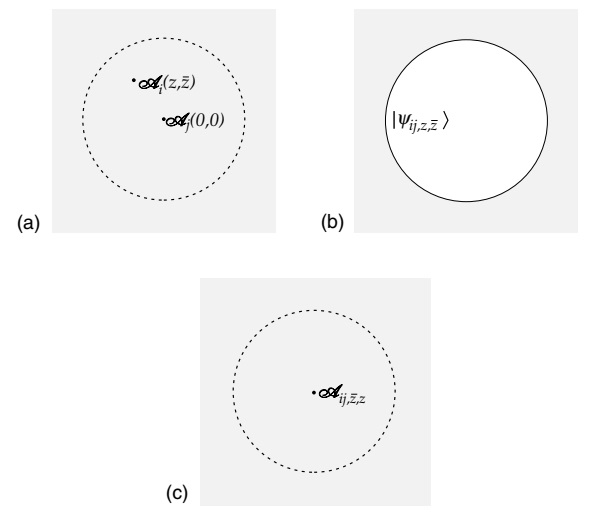
\includegraphics[width=0.8\textwidth]{figure/Fig2.7.jpg}
		\caption{(a) Worldsheet with two local operators. (b) Integrating over fields inside the disk gives boundary state $\lvert\psi_{i j, z, \bar{z}}\rangle$. (c) Cutout inside a disk with corresponding local operators. Expanding to operators with definite weights gives OPE.    }\label{Fig2.7}
	\end{center}
\end{figure}
Examine product    
\begin{equation}
	\mathscr{A}_{i}(z, \bar{z}) \mathscr{A}_{j}(0,0) \:, \label{2.9.1}
\end{equation}
where $|z|<1$. We can split the path integral into integration over field $\phi_{\mathrm{i}}$ inside unit circle, field $\phi_{\mathrm{b}}$ on unit circle, field $\phi_{\mathrm{e}}$ outside unit circle.    
As discussed at the end of last section, integration over $\phi_{\mathrm{i}}$ yields some functional of $\phi_{\mathrm{b}}$, denoted as $\Psi_{i j, z, \bar{z}}[\phi_{\mathrm{b}}]$. Via state--operator correspondence, this is equivalent to gluing disk together with appropriate operator $\mathscr{A}$. To turn it into standard form expanded with complete set of $L_{0}, \tilde{L}_{0}$ eigenstates    
\begin{equation}
	\mathscr{A}_{i j, z, \bar{z}}=\sum_{k} z^{h_{k}-h_{i}-h_{j}}\bar{z}^{\tilde{h}_{k}-\tilde{h}_{i}-\tilde{h}_{j} }c^{k}{}_{i j} \mathscr{A}_{k} \:, \label{2.9.2}
\end{equation}
where $z$ dependence and $\bar{z}$ dependence are determined by conformal weights like (\ref{2.4.20}).   
\begin{tcolorbox}[breakable]
\begin{proof} 
We consider the product of two operators acting on the vacuum. In radial quantization, $\mathcal{A}_j(0,0)$ creates a state at the origin, and $\mathcal{A}_i(z,\bar{z})$ acts as an operator on the Hilbert space at radius $|z|$.
\begin{equation}
	|\Psi_{ij}(z,\bar{z})\rangle = \mathcal{A}_i(z,\bar{z}) \mathcal{A}_j(0,0) |0\rangle = \mathcal{A}_i(z,\bar{z}) |\mathcal{A}_j\rangle
\end{equation}
Since $\{|\mathcal{A}_k\rangle = \mathcal{A}_k(0,0)|0\rangle\}$ forms a complete basis for the Hilbert space, we expand the state $|\Psi\rangle$:
\begin{equation}
	|\Psi_{ij}(z,\bar{z})\rangle = \sum_k C_{ij}^k(z,\bar{z}) |\mathcal{A}_k\rangle
\end{equation}
To find the $z$-dependence, we apply the dilatation generator $L_0$. For a primary operator $\mathcal{A}_i$ with weight $h_i$, the commutator is:
\begin{equation}
	[L_0, \mathcal{A}_i(z,\bar{z})] = (z \partial_z + h_i) \mathcal{A}_i(z,\bar{z})
\end{equation}
Applying $L_0$ to the state $|\Psi_{ij}\rangle$ and using $L_0 |\mathcal{A}_j\rangle = h_j |\mathcal{A}_j\rangle$:
\begin{align}
	L_0 |\Psi_{ij}(z,\bar{z})\rangle &= L_0 \mathcal{A}_i(z,\bar{z}) |\mathcal{A}_j\rangle \notag\\
	&= [L_0, \mathcal{A}_i(z,\bar{z})] |\mathcal{A}_j\rangle + \mathcal{A}_i(z,\bar{z}) L_0 |\mathcal{A}_j\rangle\notag \\
	&= (z \partial_z + h_i + h_j) |\Psi(z,\bar{z})\rangle
\end{align}

Applying $L_0$ to the basis expansion side:
\begin{equation}
	L_0 \sum_k C_{ij}^k(z,\bar{z}) |\mathcal{A}_k\rangle = \sum_k h_k C_{ij}^k(z,\bar{z}) |\mathcal{A}_k\rangle
\end{equation}
Equating both sides, the coefficients $C_{ij}^k$ must satisfy:
\begin{equation}
	(z \partial_z + h_i + h_j) C_{ij}^k(z,\bar{z}) = h_k C_{ij}^k(z,\bar{z})
\end{equation}
Rearranging gives the scaling equation:
\begin{equation}
	z \partial_z C_{ij}^k = (h_k - h_i - h_j) C_{ij}^k
\end{equation}
The solution is:
\begin{equation}
	C_{ij}^k(z,\bar{z}) = c_{ij}^k z^{h_k - h_i - h_j} \bar{z}^{\bar{h}_k - \bar{h}_i - \bar{h}_j}
\end{equation}

Stripping the vacuum state, we recover the OPE in its standard form:
\begin{equation}
	\mathcal{A}_i(z,\bar{z}) \mathcal{A}_j(0,0) = \sum_k c_{ij}^k z^{h_k - h_i - h_j} \bar{z}^{\bar{h}_k - \bar{h}_i - \bar{h}_j} \mathcal{A}_k(0,0)
\end{equation}
	QED.
\end{proof}
\end{tcolorbox} 
Convergence of OPE is exactly convergence of a complete set in quantum mechanics. As long as there is no other operator in $\lvert z^{\prime}\rvert \leq \lvert z\rvert$, this construction is possible. Allowing us to cut out circle of radius $|z|+\epsilon$.    
For three operators    
\begin{equation}
	\mathscr{A}_{i}(0,0) \mathscr{A}_{j}(1,1) \mathscr{A}_{k}(z, \bar{z}) \:, \label{2.9.3}
\end{equation}
convergence region $|z|<1$ of $z\to 0$ OPE overlaps with convergence region $|1-z|<1$ of $z\to 1$ OPE. Then coefficient of $\mathscr{A}_l$ in triple product can be written as summation including $c^{l}{}_{i k} c^{m}{}_{l j}$ or summation including $c^{l}{}_{j k} c^{m}{}_{li}$. Associativity requires these sums to be equal.    
Graphic representation see Figure \ref{Fig2.8}.    
\begin{figure}[!htbp]
	\begin{center}
		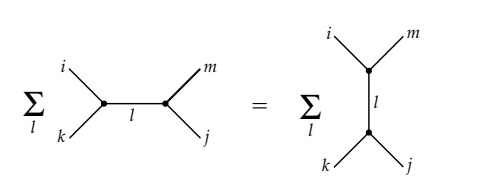
\includegraphics[width=0.8\textwidth]{figure/Fig2.8.jpg}
		\caption{Graphical representation of OPE associativity    }\label{Fig2.8}
	\end{center}
\end{figure}

\subsection*{Virasoro Algebra and Highest Weight States}

Now apply discussion in Figure \ref{Fig2.6} to Virasoro generators:    
\begin{align}
	L_{m}\lvert \mathscr{A}\rangle & \cong \oint \frac{\dif z}{2 \pi \mi}\: z^{m+1} T(z) \mathscr{A}(0,0)  \nonumber \\
	& \cong L_{m} \cdot \mathscr{A}(0,0) \:.
	\label{2.9.4}
\end{align}
Here we entered new notation and concept. Given state-operator isomorphism, each operator acting on Hilbert space has an image acting on local operator space. In other words, formed corresponding contour around operator and calculated corresponding local operator using OPE. Corresponding to $L_m$ mapping states to states is $L_m\cdot$ mapping local operators to local operators. Generally there will be local operators at different positions $z_i$, and each position will have a different version of Virasoro algebra. These different versions are obtained by Laurent expansion centered at operator position. A standard basis for generators will also exist in some geometries.    
For example for cylinder then expansion centered at $z=0$. "$\cdot$" acts as a reminder: what we discuss is Laurent expansion coefficient around specific operator.    

In this notation, $T\mathscr{A}$ OPE is    
\begin{equation}\label{2.9.5}
	T(z) \mathscr{A}(0,0)=\sum_{m=-\infty}^{\infty} z^{-m-2} L_{m} \cdot \mathscr{A}(0,0) \:.
\end{equation}
To relate to earlier notation (\ref{2.4.11}), for $n \geq 0$, $\mathscr{A}^{(n)}=L_{n-1} \cdot \mathscr{A}$, conformal transformation of $\mathscr{A}$ is    
\begin{equation}
	\delta \mathscr{A}(z, \bar{z})=-\epsilon \sum_{n=0}^{\infty} \frac{1}{n !}\Bigl[\partial^{n} v(z) L_{n-1}+\left(\partial^{n} v(z)\right)^{*} \tilde{L}_{n-1}\Bigr] \cdot \mathscr{A}(z, \bar{z}) \:.
	\label{2.9.6}
\end{equation}
Using general form of $T\mathscr{A}$ OPE (\ref{2.4.14}), we have very useful results    
\begin{subequations}\label{2.9.7}
	\begin{align}
		L_{-1} \cdot \mathscr{A}&=\partial \mathscr{A}, \quad \tilde{L}_{-1} \cdot \mathscr{A}=\bar{\partial} \mathscr{A} \:, \label{2.9.7a} \\
		L_{0} \cdot \mathscr{A}&=h \mathscr{A}, \quad \tilde{L}_{0} \cdot \mathscr{A}=\tilde{h} \mathscr{A} \:.\label{2.9.7b}
	\end{align}
\end{subequations}
OPE (\ref{2.9.5}) implies state corresponding to primary field $\mathcal{O}$ with weight $(h, \tilde{h})$ satisfies    
\begin{subequations} \label{2.9.8}
	\begin{align}
		L_{0}|\mathcal{O}\rangle&=h|\mathcal{O}\rangle \:, \quad \tilde{L}_{0}|\mathcal{O}\rangle=\tilde{h}|\mathcal{O}\rangle \:, \label{2.9.8a} \\
		L_{m}|\mathcal{O}\rangle&=\tilde{L}_{m}|\mathcal{O}\rangle=0\:, \quad m>0 \:.
		\label{2.9.8b}
	\end{align}
\end{subequations}
Such state is called highest weight state: by repeatedly acting with lowering operators on arbitrary state, we eventually obtain state annihilated by further lowering operators, called highest weight state.    

An interesting special case is identity operator, operator product $T1$ is non-singular, so in arbitrary CFT get    
\begin{equation}
	L_{m}|1\rangle=\tilde{L}_{m}|1\rangle=0, \quad m \geq-1 \:.
	\label{2.9.9}
\end{equation}
As marked in 2.4, operators $L_{0}$ and $L_{\pm 1}$ form closed algebra, so do $\tilde{L}_{0}$ and $\tilde{L}_{\pm 1}$. Entire algebra is    
\begin{equation}
	SL(2,\mathds{R})\times SL(2,\mathds{R})= S L(2, \mathds{C}) \:. \label{2.9.10}
\end{equation}
Therefore $|1\rangle$ is also called $SL(2, \mathds{C})$-invariant state.    
It is the only such state, because (\ref{2.9.7}) implies any operator $\mathscr{A}$ corresponding to $SL(2, \mathds{C})$-invariant state is independent of position, so must be $c$-number, as explained after (\ref{2.4.24}).    

\subsection*{Unitary CFT}

Highest weight states play important role in string theory and representation theory of Virasoro algebra. Now we derive several important results generally valid in unitary CFT.    
Unitary CFT has positive definite inner product, making    
\begin{equation}
	L_{m}^{\dagger}=L_{-m} \: , \quad \tilde{L}_{m}^{\dagger}=\tilde{L}_{-m} \:. \label{2.9.11}
\end{equation}
Recall: inner product via $\langle\alpha \vert A \beta\rangle=\langle A^{\dagger} \alpha \vert \beta\rangle$ defined adjoint.    
For example $X^\mu$ CFT for \emph{spacelike} $\mu$ is unitary. If we take inner product of ground states as    
\begin{equation}
	\langle 0 ; k \vert 0 ;
	k^{\prime} \rangle=2 \pi \delta(k-k^{\prime})  \label{2.9.12}
\end{equation} 
and define    
\begin{equation}
	\alpha_{m}^{\dagger}=\alpha_{-m} \:, \quad \tilde{\alpha}_{m}^{\dagger}=\tilde{\alpha}_{-m} \:. \label{2.9.13}
\end{equation}
This implicitly defines inner product of all higher states. This CFT for $X^\mu=0$ is not unitary, because there is negative sign in commutation relation there.    

First constraint in unitary CFT is any state must have $h, \tilde{h} \geq 0$.    
If this holds for highest weight states, then it holds for all states. For highest weight states, Virasoro algebra gives    
\begin{equation}\label{2.9.14}
	2 h_{\mathcal{O}}\langle\mathcal{O} \vert \mathcal{O}\rangle=2\langle\mathcal{O}\vert L_{0}\vert \mathcal{O}\rangle=\langle\mathcal{O}|[L_{1}, L_{-1}]|\mathcal{O}\rangle=\| L_{-1}|\mathcal{O}\rangle \|^{2} \geq 0 \:,
\end{equation}
so $h_{\mathcal{O}} \geq 0 $.    
If $h_{\mathcal{O}}=\tilde{h}_{\mathcal{O}}=0$, then    
\begin{equation}
	L_{-1} \cdot \mathcal{O}=\tilde{L}_{-1} \cdot \mathcal{O}=0 \:, \label{2.9.15}
\end{equation}
thus $\mathcal{O}$ is independent of position. As previously marked, $\mathcal{O}$ must be $c$-number, i.e., in unitary CFT identity operator is unique $(0,0)$ operator. Surprisingly, $X^\mu$ is unique exception: corresponding state $x^{\mu}|0 ;
0\rangle$ is non-normalizable due to infinite range of $X^\mu$, and equation (\ref{2.9.14}) no longer holds.    
For CFT corresponding to compact dimension, general theorem is most useful, such exceptions cannot occur.    

In same way, in unitary CFT, if and only if $\tilde{h}=0$, operator is holomorphic, and if and only if $h=0$, operator is anti-holomorphic;    
this is an important result, repeated as follows:    
\begin{equation}
	\partial \mathscr{A}=0 \Leftrightarrow h=0 \:, \quad \bar{\partial} \mathscr{A}=0 \Leftrightarrow \tilde{h}=0 \:. \label{2.9.16}
\end{equation}
Finally, using previous discussion and commutator $\left[L_{n}, L_{-n}\right]$ it can be proven that in unitary CFT $c, \tilde{c} \geq 0$.    
Actually, unique unitary CFT with $c=0$ is trivial: $L_n=0$.    

\subsection*{Zero-point energy}
State-operator mapping gives another simple derivation of different normal-ordering constants. In any CFT, we know $L_{0}|1\rangle=0$, and this determines another normalization of $L_0$.    
In $X$ CFT, $|1\rangle=0$ is ground state, so $a^X=0$.    
In $bc$ theory, $|1\rangle=0$ is excited state $b_{-1}\lvert \downarrow\rangle$, so to be consistent with earlier $\lambda=2$ result (\ref{2.7.1}), weight of $\lvert \downarrow\rangle$ is $-1$.    

This also provides physical interpretation of central charge. In unitary CFT, ground state is $|1\rangle$ with $L_{0}=\tilde{L}_{0}=0$.    
Conformal transformation (\ref{2.6.10}) between radial generator and time translation generator implies for ground state    
\begin{equation}
	E=-\frac{c+\tilde{c}}{24} \:.
	\label{2.9.17}
\end{equation}
This is Casimir energy, arising from finite scale of system, and dependent on central charge. Based on dimensional analysis, this energy is inversely proportional to size $\ell$ of system, here $2\pi$, so general result is    
\begin{equation}
	E=-\frac{\pi(c+\tilde{c})}{12 \ell} \:. \label{2.9.18}
\end{equation}
We now have three ways to calculate normal-ordering constants:    
\begin{enumerate}
	\item Like in (\ref{2.7.8}), starting from Virasoro algebra;
	\item Like in (\ref{2.7.11}), relating two forms of normal ordering;
	\item Starting from previous state-operator mapping.    
\end{enumerate}
However method of adding up zero-point energy is intuitive, so we give another description:    
\begin{enumerate}
	\item For each boson mode, zero-point energy is $\frac{1}{2} \omega$; for each fermion mode, zero-point energy is $-\frac{1}{2} \omega$. Add up energy.
	\item Encountering divergent sum of form $\sum_{n=1}^{\infty}(n-\theta)$, where $\theta$ comes from non-trivial periodicity conditions, define it as    
	\begin{equation}
		\sum_{n=1}^{\infty}(n-\theta)=\frac{1}{24}-\frac{1}{8}(2 \theta-1)^{2} \:. \label{2.9.19}
	\end{equation}
	This value can be obtained, as in \eqref{1.3.32}, by regularizing and discarding the quadratically divergent part. 
	\item The normal ordering constant for the generator $T_0$ in the $w$ frame was provided earlier, where $T_0$ is defined by (\ref{2.6.8}). 
	For $L_0$, we must add the non-tensor correction $\frac{1}{24} c$. 
\end{enumerate}
For the free bosonic field, the modes are integer-valued; thus, after step 2, for $\theta=0$, we obtain half of the sum, which is $-\frac{1}{24}$.  This is exactly canceled by the correction in step 3, giving $a^X=0$.  For the ghost fields, we similarly obtain $\frac{2}{24}-\frac{26}{24}=-1$.
	% \setcounter{section}{0}% Change the chapter counter value
% %\numberwithin{equation}{chapter}% Equation counter follows chapter
% \numberwithin{equation}{section}% Equation counter follows section
% %\numberwithin{figure}{section}% Figure counter follows section
% \setcounter{chapter}{2}

\chapter{\texorpdfstring{The Polyakov path integral}{3 The Polyakov path integral}} \label{cha:3}

We now undertake a systematic study of string theory using the Polyakov path integral and conformal field theory. After introducing the path integral picture, we discuss gauge fixing, the Weyl anomaly, and vertex operators. Subsequently, we will generalize string theory to curved spacetime.

\section{\texorpdfstring{Sums over world-sheets}{3.1 Sums over world-sheets}} \label{sec:3.1}
The Feynman path integral is one way to represent quantum theory, and it is a very natural method for describing string interactions. In path integral quantization, amplitudes are obtained by summing over all possible histories between initial and final states. Each history is assigned a weight    
\begin{equation}
	\exp (\mi S_{\mathrm{cl}} / \hbar) \:, \label{3.1.1}
\end{equation}
where $S_{\mathrm{cl}}$ is the classical action for the given history. Thus, summing over all worldsheets connecting given initial and final curves defines the amplitude in string theory. Figure \ref{Fig3.1}a refers to open strings, and Figure \ref{Fig3.1}b to closed strings. A similar sum for a relativistic point particle yields the free propagator.    
\vspace{-0.5cm}
\begin{figure}[!htbp]
	\begin{center}
		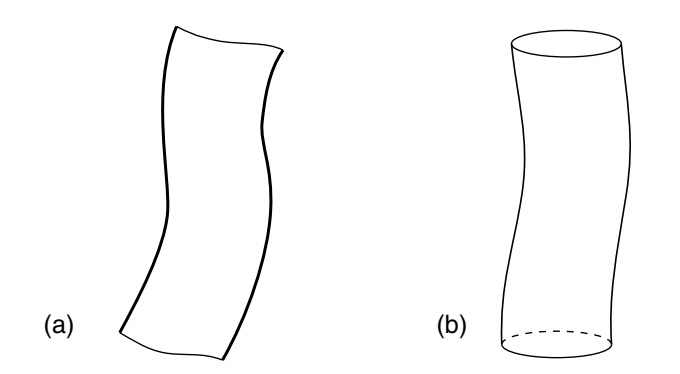
\includegraphics[width=0.8\textwidth]{figure/Fig3.1.jpg}
		\caption{(a) Open string worldsheet with the topology of a long strip. The bold curves are the worldlines of the string endpoints. (b) Closed string worldsheet with the topology of a cylinder.    }\label{Fig3.1}
	\end{center}
\end{figure}

One can imagine several ways for strings to interact. One is a contact interaction, the energy when two strings intersect; another is through long-range forces via some quantum field. However, interactions added manually to string theory cannot be consistent with symmetry; we will see the reasons for this later.    
Conversely, the only allowed interaction is already implicit in the sum over worldsheets. For example, consider the worldsheets shown in Figure \ref{Fig3.2}. Figure \ref{Fig3.2}a looks like a quantum correction to the open string amplitude in Figure \ref{Fig3.1}a. This correction includes an intermediate state with two open strings. Figure \ref{Fig3.2}b has three external closed strings, representing a string decaying into two. From this, we see that this is a correct way to introduce interactions in strings. We will see that these interactions produce consistent theories containing gravity that are finite and unitary.    
\begin{figure}[!htbp]
	\begin{center}
		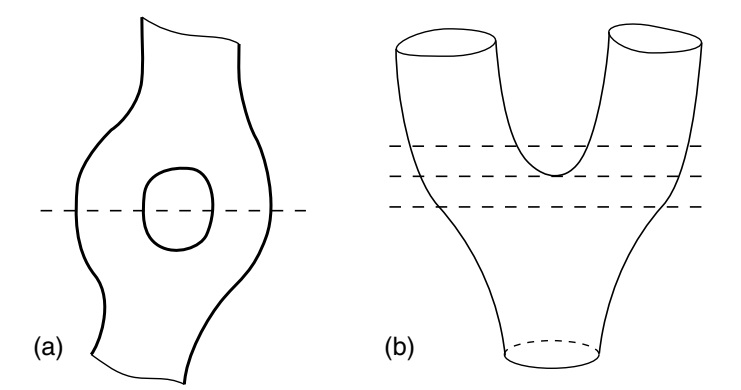
\includegraphics[width=0.75\textwidth]{figure/Fig3.2.jpg}\\
		\caption{(a) Quantum correction to the open string propagator. (b) A closed string decaying into two. Dashed lines represent time slices.    }\label{Fig3.2}
	\end{center}
\end{figure}

It is interesting to examine the process of Figure \ref{Fig3.2}b at several consecutive moments, as shown in Figure \ref{Fig3.3}.    
\begin{figure}[!htbp]
	\begin{center}
		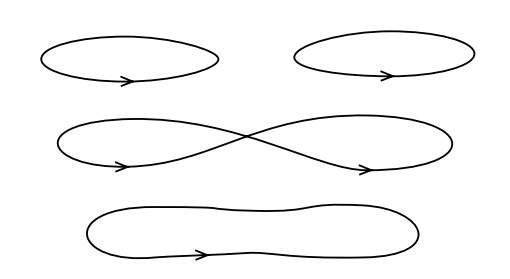
\includegraphics[width=0.65\textwidth]{figure/Fig3.3.jpg}\\
		\caption{Several consecutive slices of Figure \ref{Fig3.2}b. Arrows indicate the orientation of the string.    }\label{Fig3.3}
	\end{center}
\end{figure}
In closed string theory, all particles are obtained as different vibrational states of the string. All interactions (gauge, gravitational, Yukawa) originate from the single process in Figure \ref{Fig3.3}. For theories with open strings, there are several additional possible processes, as shown in Figure \ref{fig:3.4}. At a given moment, the processes in Figures \ref{Fig3.3} and \ref{fig:3.4} occur at definite spacetime points, but this is an illusion. A different slicing places the apparent interaction at different points; there are no distinguishable points in spacetime. Interactions originate only from the global topology of the worldsheet, while the local properties of the worldsheet are the same as in the free case.    
As discussed in the introduction, this "smeared out" interaction cuts off short-distance divergences in gravity.    
\vspace{0.5cm}
\begin{figure}[!htbp]
	\begin{center}
		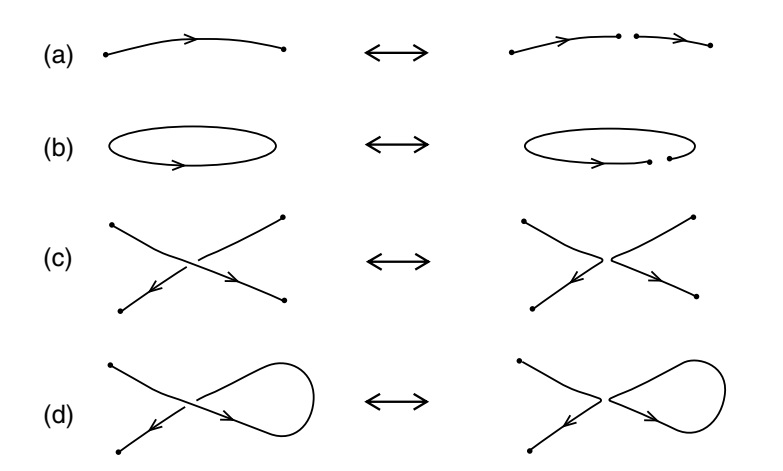
\includegraphics[width=0.7\textwidth]{figure/Fig3.4.jpg}\\
		\caption{Processes involving open strings: (a) open string $\leftrightarrow$ open string $+$ open string; (b) closed string $\leftrightarrow$ open string;     (c) open string $+$ open string $\leftrightarrow$ open string $+$ open string; (d) open string $\leftrightarrow$ open string $+$ closed string.    }\label{fig:3.4}
	\end{center}
\end{figure}

In fact, there are several different string theories, depending on the topologies introduced in the sum over worldsheets. Note that the worldsheets we have drawn have two types of boundaries: source boundaries corresponding to the initial and final string configurations, and endpoint boundaries corresponding to the worldlines of the open string ends. For now, ignore the source boundaries; we will discuss source details later in this chapter.    
Therefore, in subsequent discussions, "boundary" refers to the endpoint boundary. Thus, there are 4 ways to define the sum over worldsheets, corresponding to the 4 free string theories listed at the end of Section 1.4:    
\begin{enumerate}
	\item Closed oriented: all oriented worldsheets without boundaries; 
	\item Closed unoriented: all worldsheets without boundaries; 
	\item Closed plus open oriented: all oriented worldsheets with any number of boundaries; 
	\item Closed plus open unoriented: all worldsheets with any number of boundaries; 
\end{enumerate} 


\begin{figure}[!htbp]
	\begin{center}
		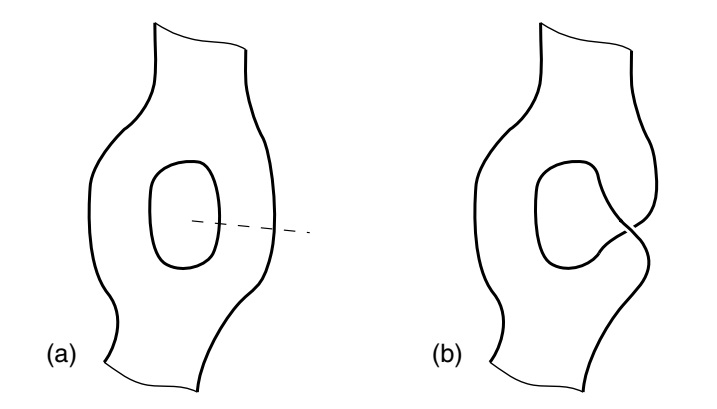
\includegraphics[width=0.65\textwidth]{figure/Fig3.5.jpg}\\
		\caption{Oriented (a) and unoriented (b) contributions to the 2-open-string amplitude.    }\label{Fig3.5}
	\end{center}
\end{figure}

There are two things to elaborate on here.    
One is the connection between the inclusion of unoriented worldsheets and the $\Omega=+1$ projection described in Section 1.4. Figure \ref{Fig3.5} shows two worldsheets counted in the open unoriented theory. The worldsheet in Figure \ref{Fig3.5}b is equivalent to cutting Figure \ref{Fig3.5}a along the dashed line. We parameterize it with $0 \leq \sigma \leq \pi$ and require the fields at the cut to satisfy    
\begin{equation}
	X_{\text {upper }}^{\mu}(\sigma)=X_{\text {lower }}^{\mu}(\pi-\sigma) \:. \label{3.1.2}
\end{equation}
This in turn is equivalent to acting with the operator $\Omega$ on the open string states. Summing these two surfaces with appropriate weights is equivalent to inserting the operator $\frac{1}{2}(1+\Omega)$, which projects onto $\Omega=+1$ states.    
In the sum over all oriented and unoriented surfaces, inserting projection operators on all intermediate states reduces the spectrum to the $\Omega=+1$ part.    

\begin{figure}[!htbp]
	\begin{center}
		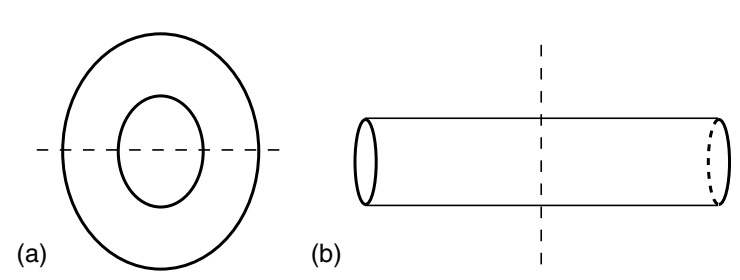
\includegraphics[width=0.8\textwidth]{figure/Fig3.6.jpg}\\
		\caption{(a) Annulus: the intermediate state consists of two open strings. (b) Cylinder with the same topology: the intermediate state is a single closed string.    }\label{Fig3.6}
	\end{center}
\end{figure}

Second, the list above does not include a theory with only open strings. Let's explain in detail why this is the case.    
Consider a worldsheet with the topology of an annulus, as shown in Figure \ref{Fig3.6}a. For convenience, we have only drawn the vacuum amplitude, but the same discussion applies to scattering amplitudes by connecting appropriate sources.    
As can be seen from the dashed lines, this is a process with two open strings in the intermediate state. Thus, worldsheets of this topology must appear in any theory with open strings. In Figure \ref{Fig3.6}b, we draw the same topology as a cylinder and cut it at an intermediate state of a single closed string.    
Therefore, even if we start only with open strings, the sum over worldsheets will inevitably introduce such processes—the scattering of open strings produces closed strings. As we study the divergence of amplitudes, we will see in detail how this works.    

The necessity of closed strings in open string theory can be seen from another perspective. Consider the interactions in Figure \ref{fig:3.4}a and b, but time-reversed: two open strings merge into one, and an open string becomes closed. Joining them at the interaction point is the same; merging two ends allows the first interaction but not the second. This would require attaching some non-local constraints to the dynamics of the string, which would prove to be inconsistent.    
The same discussion applies to Figures \ref{fig:3.4}c and d, where the interaction is the local reconnection of a pair of strings; thus, if any open string interaction is allowed, the same process producing a closed string from open strings is also allowed.    

\section{\texorpdfstring{The Polyakov path integral}{3.2 The Polyakov path integral}} \label{sec:3.2}

We now begin to study the sum over worldsheets, expressed as a functional integral in the Polyakov formalism.    
There is a difference here from Chapter \ref{cha:1}: the Minkowski metric $\gamma_{ab}$ is replaced by the Euclidean metric $g_{a b}(\sigma^{1}, \sigma^{2})$ with signature $(+,+)$. The integral is taken over all Euclidean metrics and the embedding $X^{\mu}(\sigma^{1}, \sigma^{2})$ of the worldsheet in Minkowski spacetime:    
\begin{equation}\label{3.2.1}
	\int[\dif X \dif g] \exp (-S) \:.
\end{equation}
The Euclidean action is    
\begin{equation}
	S=S_{X}+\lambda \chi \:, \label{3.2.2}
\end{equation}
where    
\begin{subequations}\label{3.2.3}
	\begin{align}
		S_{X}&=\frac{1}{4 \pi \alpha^{\prime}} \int_{M} \dif^{2} \sigma \: g^{1 / 2} g^{a b} \partial_{a} X^{\mu} \partial_{b} X_{\mu} \:, \label{3.2.3a} \\
		\chi&=\frac{1}{4 \pi} \int_{M} \dif^{2} \sigma \: g^{1 / 2} R+\frac{1}{2 \pi} \int_{\partial M} \dif s\: k \:.
		\label{3.2.3b}
	\end{align}
\end{subequations}
Here $\dif s$ is the proper time along the boundary, and $k$ is the geodesic curvature of the boundary $k=\pm t^{a} n_{b} \nabla_{a} t^{b}$. \\    
\begin{remark}
	$t^a$ is a unit vector tangent to the boundary, and $n^a$ is a unit vector pointing outward and perpendicular to $t^a$; the $+$ sign corresponds to a timelike boundary, and $-$ to a spacelike boundary. Here the boundary is always spacelike.    
\end{remark}
\begin{tcolorbox}[breakable]
	\begin{proof}
		We wish to show that the Euler term
		
		\begin{equation}
			\chi = \frac{1}{4\pi} \int_M d^2\sigma \sqrt{g}R + \frac{1}{2\pi} \int_{\partial M} ds \, k
		\end{equation}
		
		with \( k \) the geodesic curvature given by
		
		\begin{equation}
			k = \pm t^a n_b \nabla_a t^b
		\end{equation}
		
		is invariant under a Weyl rescaling. From (1.2.32) we know that under a Weyl rescaling \( g'_{ab} = e^{2\omega(\sigma)} g_{ab} \) the Riemann curvature transforms, in Euclidean spacetime, as
		
		\begin{equation}
			\sqrt{g'} R' = \sqrt{g}(R - 2\nabla^2 \omega) = \sqrt{g}(R - 2\nabla^a \partial_a \omega)
		\end{equation}
		
		We have used the fact that \( \omega \) is a scalar so the \( \nabla_a \omega = \partial_a \omega \). We also know how a connection transforms under a Weyl rescaling
		
		\begin{equation}
			\begin{aligned}
				\Gamma'\,^{a}_{bc} &= \Gamma_{bc}^a + g^{ad} (g_{cd} \partial_b \omega + g_{bd} \partial_c \omega - g_{bc} \partial_d \omega) \\
				&= \Gamma_{bc}^a + \delta^a_c \partial_b \omega + \delta^a_b \partial_c \omega - \gamma^{ad} \gamma_{bc} \partial_d \omega
			\end{aligned}
		\end{equation}
		
		The tangent and normal vectors \( t^a \) and \( n^a \) are normalised, \( g_{ab}t^at^b = \mp1 \) (with the minus sign for timelike boundaries and the plus sign for spacelike boundaries). Therefore
		
		\begin{equation}
			\mp1 = g'_{ab}t'^at'^b = e^{2\omega} t'^a t'^b
		\end{equation}
		
		and similarly for \( n^a \). This can be satisfied if
		
		\begin{equation}
			t'^a = e^{-\omega} t^a \quad \text{and} \quad n'^a = e^{-\omega} n^a
		\end{equation}
		
		From this we find that
		
		\begin{equation}
			n'_a = g'_{ab}n^b = e^{2\omega} \gamma_{ab} e^{-\omega} n^b = e^{\omega} n_a
		\end{equation}
		
		The term with the geodesic curvature then becomes
		
		\begin{equation}
			\begin{aligned}
				k' &= \pm t'^a n'_b \nabla_a t'^b = \pm t'^a n'_b (\partial_a t'^b + \Gamma^b_{ac} t'^c) \\
				&= \pm e^{-\omega} t^a e^{\omega} n_b \left[ \partial_a (e^{-\omega} t^b) + (\Gamma^b_{ac} + \delta^b_c \partial_a \omega + \delta^b_a \partial_c \omega - \gamma^{bd} \gamma_{ac} \partial_d \omega) e^{-\omega} t^c \right] \\
				&= \pm t^n n_b e^{-\omega} \left( -\partial_a \omega t^b + \partial_a t^b + \Gamma^b_{ac} t^c + \partial_a \omega t^b + \delta^b_a \partial_c \omega t^c - \gamma^{bd} \gamma_{ac} \partial_d \omega t^c \right) \\
				&= e^{-\omega} (k \mp t^a n_b \gamma^{bd} \gamma_{ac}  t^c\partial_d \omega) = e^{-\omega} (k \mp t^a t_a n_b \partial^b \omega)
			\end{aligned}
		\end{equation}
		
		where we have used that the tangent and normal vectors are orthonormal \( t^a n_a = 0 \). Now, if \( t^a t_a = -1 \) then we are to chose the upper sign, which is minus and so the second term in the brackets gets a plus sign. If \( t^a t_a = +1 \) we need to take the lower sign and we once again find a plus sign for the second term. Thus
		
		\begin{equation}
			k' = e^{-\omega} (k + n^a \partial_a \omega)
		\end{equation}
		
		It remains to work out the transformation of \( ds \). We have
		
		\begin{equation}
			ds'^2 = g'_{ab} dx^a dx^b = e^{2\omega} dx^a dx^b = e^{2\omega} ds^2
		\end{equation}
		
		and thus
		
		\begin{equation}
			ds' = e^{\omega} ds
		\end{equation}
		
		Bringing everything together we have
		
		\begin{equation}
			\begin{aligned}
				\chi' &= \frac{1}{4\pi} \int_M d^2 \sigma \sqrt{g'} R' + \frac{1}{2\pi} \int_{\partial M} ds' k' \\
				&= \frac{1}{4\pi} \int_M d^2 \sigma \sqrt{g} (R - 2\nabla^2 \omega) + \frac{1}{2\pi} \int_{\partial M} e^{\omega} dse^{-\omega} (k + n^a \partial_a \omega) \\
				&= \frac{1}{4\pi} \int_M d^2 \sigma \sqrt{g} R + \frac{1}{2\pi} \int_{\partial M} ds k + \frac{1}{2\pi} \left[ -\int_M d^2 \sigma \sqrt{g} \nabla^a \partial_a \omega + \int_{\partial M} ds n^a \partial_a \omega \right] \\
				&= \chi
			\end{aligned}
		\end{equation}
		
		where the term between brackets vanishes due to Stokes' theorem
		
		\begin{equation}
			\int_M d^2 \sigma \sqrt{g} \nabla^a v_a = \int_{\partial M} ds n^a v_a
		\end{equation}
	\end{proof}
\end{tcolorbox}
The advantage of the Euclidean path integral is that the integral over the metric is better defined. The topologically non-trivial worldsheets we describe can have non-singular Euclidean metrics, whereas Minkowski metrics cannot. We will take the Euclidean theory \eqref{3.2.1} as the starting point. We will show how to give it a precise definition and that it defines a consistent spacetime theory.    
However, we will give a brief formal discussion that it is equivalent to our starting point Minkowski theory.    

We start with the point particle example, where the path integral    
\begin{equation}
	\int[\dif X] \exp \left[iS_{\rm NG}\right]=\int[\dif \eta \, \dif X] \exp \left[\frac{\mi}{2} \int \dif \tau\: \Bigl(\eta^{-1} \dot{X}^{\mu} \dot{X}_{\mu}-\eta m^{2}\Bigr)\right] \label{3.2.4}
\end{equation}
is oscillatory.  

\begin{tcolorbox}[breakable]
	Both Nambu-Goto and Polyakov action have gauge redundancy, therefore to show that the partition function are equivalent we define the Euclidean action for a free relativistic particle of mass $m$ propagating in a $D$-dimensional flat spacetime using the auxiliary einbein formalism:
	\begin{equation}
		S[X, e] = \int_{0}^{1} d\tau \left( \frac{\dot{X}^2}{2e(\tau)} + \frac{1}{2} e(\tau) m^2 \right)
	\end{equation}
	where:
	\begin{itemize}
		\item $\tau \in [0, 1]$ is the arbitrary parameter along the worldline.
		\item $X^\mu(\tau)$ are the target-space coordinates.
		\item $\dot{X}^2 = \delta_{\mu\nu} \frac{dX^\mu}{d\tau} \frac{dX^\nu}{d\tau}$ is the squared worldline velocity.
		\item $e(\tau)$ is the einbein (the 1D independent metric component, intrinsically local).
	\end{itemize}
	The path integral requires integrating over all field configurations. 
	\[
	Z = \int \mathcal{D}x \, \mathcal{D}e \; \exp\left( -S \right).
	\]
	The measure for $\mathcal{D}e$ is found by requiring that the diffeomorphism-invariant measure be defined by the following normalization condition:\footnote{This part mirrors section 3.1.2 of Roberto Perccaci's Asymptotic Safety textbook.}
	\begin{equation}
		1 = \int \mathcal{D}(\delta e) \mu_e \exp\left( -\|\delta e\|^2 \right)
	\end{equation}
	We consider the fluctuation $\delta e$ rather than the field $e$ itself because, although the global field manifold is non-linear, the tangent space at any given configuration is locally flat. This flatness is what allows us to validly apply Gaussian integration techniques to determine the functional measure. Consider the reparameterization invariant norm for fluctuations $\delta e$:
	\begin{equation}
		\|\delta e\|^2 = \int d\tau G(e) (\delta e)^2
	\end{equation}
	
	Under a transformation $\tau \to \tau'$, let $J = \frac{d\tau'}{d\tau}$. The variables transform as:
	\begin{equation}
		d\tau' = J d\tau, \quad e = J^{-1} e, \quad \delta e = J^{-1} \delta e
	\end{equation}
	
	Requirement for invariance of the norm:
	\begin{equation}
		\int (J d\tau') G(J^{-1} e) (J^{-1} \delta e)^2 = \int d\tau' G(e) (\delta e)^2
	\end{equation}
	
	For the $J$ factors to cancel out, the following scaling relation must hold:
	\begin{equation}
		J \cdot G(J^{-1} e) \cdot J^{-2} = G(e) \implies J^{-1} G(J^{-1} e) = G(e)
	\end{equation}
	
	Setting $G(e) = e^{-n}$, we solve for $n$:
	\begin{equation}
		J^{-1} (J^{-1} e)^{-n} = e^{-n} \implies J^{-1+n} = 1 \implies n = 1
	\end{equation}
	Thus, we define the invariant norm for fluctuations $\delta e$ on the worldline as:
	\begin{equation}
		\|\delta e\|^2 = \int d\tau \frac{(\delta e)^2}{e}
	\end{equation}
	
	Discretizing the worldline into $N$ intervals of width $\epsilon$:
	\begin{equation}
		\|\delta e\|^2 \approx \sum_{i=1}^N \epsilon \frac{(\delta e_i)^2}{e_i}
	\end{equation}
	
	Substituting the discretized norm and the measure $\mathcal{D}(\delta e) = \prod_{i=1}^N d(\delta e_i)$ into the normalization equation:
	\begin{equation}
		1 = \mu_e \prod_{i=1}^N \int_{-\infty}^{\infty} d(\delta e_i) \exp\left( - \frac{\epsilon}{e_i} (\delta e_i)^2 \right)
	\end{equation}
	
	Performing the Gaussian integration for each slice $i$:
	\begin{equation}
		\int_{-\infty}^{\infty} d(\delta e_i) \exp\left( - \frac{\epsilon}{e_i} (\delta e_i)^2 \right) = \sqrt{\frac{\pi e_i}{\epsilon}}
	\end{equation}
	
	Solving for the local measure $\mu_e$ (and absorbing constant factors into normalization):
	\begin{equation}
		\mu_e \propto \prod_{i=1}^N e_i^{-1/2}
	\end{equation}
	
	Thus, the discrete functional measure is:
	\begin{equation}
		\mathcal{D}e_N = \prod_{i=1}^N e_i^{-1/2} de_i
	\end{equation}	
	In the discretized limit, the einbein field $e(\tau)$ acts as a diagonal operator on the field space. We represent this as an $N \times N$ matrix $\mathbf{M}$:
	
	\begin{equation}
		\mathbf{M} = 
		\begin{bmatrix}
			e_1 & 0 & 0 & \dots & 0 \\
			0 & e_2 & 0 & \dots & 0 \\
			0 & 0 & e_3 & \dots & 0 \\
			\vdots & \vdots & \vdots & \ddots & \vdots \\
			0 & 0 & 0 & \dots & e_N
		\end{bmatrix}
	\end{equation}
	
	The functional determinant corresponds to the product of the diagonal entries:
	\begin{equation}
		\text{Det}(e) = \det(\mathbf{M}) = \prod_{i=1}^N e_i
	\end{equation}
	
	Consequently, the measure factor $\text{Det}^{-1/2}(e)$ is represented by:
	\begin{equation}
		\text{Det}^{-1/2}(e) = \left( \prod_{i=1}^N e_i \right)^{-1/2} = \prod_{i=1}^N e_i^{-1/2}
	\end{equation}
	The total partition function evaluating the auxiliary field is:
	\begin{equation}
		Z_e[X] = \int \mathcal{D}e \exp\left( -S[X, e] \right)
	\end{equation}
	To perform the exact functional integration, we must regularize the continuous integral by discretizing the worldline $\tau$ into $N$ intervals, each of uniform width $\epsilon = d\tau = 1/N$. The fields are evaluated at discrete slices $i$: $\int\dif\tau\to\sum_{i=1}^{N}\epsilon$, $e(\tau) \to e_i$ and $\dot{X}(\tau) \to \dot{X}_i$. The continuum action $S$ and measure $\mathcal{D}e$ become discrete limits:
	\begin{align}
		S_N &= \sum_{i=1}^N \epsilon \left( \frac{\dot{X}_i^2}{2e_i} + \frac{1}{2} e_i m^2 \right) \\
		\mathcal{D}e_N &= \prod_{i=1}^N e_i^{-1/2} de_i
	\end{align}
	Upon Substituting the discrete forms back into the partition function, the exponential factorizes into a product of independent, D integrals evaluated at each slice:
	\begin{equation}
		Z_{e, N}[X] = \prod_{i=1}^N \left[ \int_{0}^{\infty} \frac{de_i}{\sqrt{e_i}} \exp\left( - \frac{\epsilon \dot{X}_i^2}{2e_i} - \frac{\epsilon m^2 e_i}{2} \right) \right]
	\end{equation}

	We evaluate the integral enclosed in the square brackets using the exact mathematical identity for the modified Bessel function of the second kind:
	\begin{equation}
		\int_{0}^{\infty} x^{-1/2} \exp\left(-\frac{A}{x} - Bx\right) dx = \sqrt{\frac{\pi}{B}} \exp\left(-2\sqrt{AB}\right)
	\end{equation}
	For a single local slice $i$, we define the constants $A = \frac{\epsilon \dot{X}_i^2}{2}$ and $B = \frac{\epsilon m^2}{2}$.\\
	We evaluate the exponent for the slice:
	\begin{equation}
		-2\sqrt{AB} = -2 \sqrt{ \left(\frac{\epsilon \dot{X}_i^2}{2}\right) \left(\frac{\epsilon m^2}{2}\right) } = -2 \sqrt{ \frac{\epsilon^2 m^2 \dot{X}_i^2}{4} } = -m \epsilon \sqrt{\dot{X}_i^2}
	\end{equation}
	We evaluate the prefactor for the slice:
	\begin{equation}
		\sqrt{\frac{\pi}{B}} = \sqrt{\frac{2\pi}{\epsilon m^2}}
	\end{equation}
	Substitute the evaluated local terms back into the global discrete product:
	\begin{equation}
		Z_{e, N}[X] = \prod_{i=1}^N \left[ \sqrt{\frac{2\pi}{\epsilon m^2}} \exp\left( -m \epsilon \sqrt{\dot{X}_i^2} \right) \right]
	\end{equation}
	Separate the prefactors from the exponential sum:
	\begin{equation}
		Z_{e, N}[X] = \left( \prod_{i=1}^N \sqrt{\frac{2\pi}{\epsilon m^2}} \right) \exp\left( -m \sum_{i=1}^N \epsilon \sqrt{\dot{X}_i^2} \right)
	\end{equation}
	The infinite product of prefactors evaluates to an overall, field-independent normalization constant $\mathcal{N}_N$. Taking the continuum limit as $N \to \infty$ and $\epsilon \to d\tau$, the discrete sum over slices perfectly restores the continuous Riemann integral over the worldline:
	\begin{equation}
		\lim_{N \to \infty} Z_{e, N}[X] = \mathcal{N} \exp\left( -m \int_{0}^{1} d\tau \sqrt{\dot{X}^2} \right)
	\end{equation}
	By strictly preserving the locality of the functional measure and performing the integration slice-by-slice, the auxiliary path integral analytically collapses into the NG action $S_{\text{NG}} = m \int d\tau \sqrt{\dot{X}^2}$. 
\end{tcolorbox}
  
The path integral over $\eta, X^\mu$ is a product of ordinary integrals, so we can deform the contour just like an ordinary integral. If we take    
\begin{equation}
	\eta(\tau) \rightarrow e^{-i \theta} \eta(\tau)\:, \quad X^{0}(\tau) \rightarrow e^{-i \theta} X^{0}(\tau) \:, \label{3.2.5}
\end{equation}
for an infinitesimal $\theta$, all terms in the exponent are required to have a negative real part for convergence.    
Now we can rotate the contour in the field space $\eta=-\mi e, X^{0}=-\mi X^{D}$, and the integral becomes    
\begin{equation}
	\int[\dif e \, \dif X] \exp \Biggl[-\frac{1}{2} \int \dif \tau \: \Biggl(e^{-1} \sum_{\mu=1}^{D} \dot{X}^{\mu} \dot{X}_{\mu}+e m^{2}\Biggr)\Biggr] \:.
	\label{3.2.6}
\end{equation}
This is the Euclidean point particle analog of the path integral \eqref{3.2.1}. We have merely performed a contour rotation, so the Euclidean path integral gives the same amplitude as the Minkowski one.    

If we write the metric in the tetrad form $\gamma_{a b}=-e_{a}^{0} e_{b}^{0}+e_{a}^{1} e_{b}^{1}$ and perform the same rotation on $e_a^0$, the same treatment applies to the Polyakov action. This provides a formal proof of the equivalence of the Minkowski and Euclidean path integrals. Explicit calculations show they yield the same amplitude in the light-cone and conformal gauges. In \eqref{3.2.3a}, we left the rotation of $X^0$ to emphasize the Minkowski character of spacetime. Written in terms of $X^0$, the equations of motion and OPE are covariant with metric $\eta^{\mu\nu}$.    

We note that in two dimensions, $\chi$ is locally a total derivative, thus it depends on the topology of the worldsheet—it is the Euler characteristic of the worldsheet.    
Hence, the $\me^{-\lambda \chi}$ factor in the path integral only affects the relative weights of different topologies in the sum over worldsheets. If we add an extra strip to the worldsheet, as we did from Figure \ref{Fig3.1}a to Figure \ref{Fig3.2}a, the Euler characteristic decreases by 1, and the path integral is assigned an extra weight $\me^\lambda$. Since adding a strip corresponds to emitting and reabsorbing a virtual open string, the amplitude for emitting an open string from any process is proportional to $\me^{\lambda/2}$. Adding a handle to any worldsheet reduces the Euler characteristic by 2, thus increasing the factor by $\me^{2\lambda}$. Since this corresponds to emitting and reabsorbing a closed string, the amplitude for emitting a closed string is proportional to $\me^\lambda$.    
The Euler term in the action thus controls the coupling constants in string theory, where    
\begin{equation}\label{3.2.7}
	g_{\mathrm{o}}^{2} \sim g_{\mathrm{c}} \sim \me^{\lambda} \:.
\end{equation}
Incidentally, $\lambda$ can be viewed as a free parameter in the theory, which contradicts the statement in the introduction that string theory has no such parameters. This is a key point, and we will address it in Section \ref{sec:3.7}.    

On the other hand, the counting of couplings extends in a simple way to worldsheets with string sources. Sources for closed strings are closed loops, and sources for open strings are line segments with boundaries. For convenience, we will require the open string source boundaries to be at right angles with the endpoint boundaries in the worldsheet metric. We must be careful because the boundary curvature diverges at corners: the Euler characteristic is    
\begin{equation}
	\chi=\tilde{\chi}+\frac{1}{4} n_{\mathrm{c}} \:, \label{3.2.8}
\end{equation}
where $\tilde{\chi}$ only includes integrals over smooth boundary parts. $n_\mathrm{c}$ is the number of corners.    
The correct weight for the path integral is    
\begin{equation}\label{3.2.9}
	\exp (-\lambda \tilde{\chi})=\exp (-\lambda \chi+\lambda n_{\mathrm{c}} / 4) \:. 
\end{equation}
This stems from unitarity: if we cut the worldsheet, the $\lambda$ dependence must be invariant. This is indeed the case for weight \eqref{3.2.9}, because the area integral in $\tilde{\chi}$ cancels at the edges. Adding a closed string source is equivalent to cutting a hole in the worldsheet and reducing $\chi$ by 1.    
Adding an open string source leaves $\chi$ unchanged but increases $n_c$ by 2. Thus, we obtain the same amplitudes for emitting closed or open strings as in \eqref{3.2.7}.    

\section{\texorpdfstring{Gauge fixing}{3.3 Gauge fixing}} \label{sec:3.3}

The path integral \eqref{3.2.1} is not entirely correct, as it contains a massive overcounting. This is because configurations $(X, g)$ and $(X^{\prime}, g^{\prime})$ related by diff $\times$ Weyl symmetry represent the same physical configuration.    
In fact, we need to divide by the volume of the local symmetry group,    
\begin{equation}\label{3.3.1}
	\int \frac{[\dif X\, \dif g]}{V_{\text {diff } \times \text { Weyl }}} \exp (-S) \equiv Z \:.
\end{equation}
We will achieve this through gauge fixing, integrating over a slice that passes through each gauge equivalence class once, and obtaining the correct measure on the slice using the Faddeev-Popov method.    

In Chapter \ref{cha:1}, we applied the light-cone gauge. While useful for some purposes, this hides certain symmetries of the theory, so we now make a different choice. Note that the metric is symmetric with three independent components, and there are three gauge functions: two coordinates and the local scaling of the metric.    
Thus, there are exactly enough gauge degrees of freedom to eliminate the integral over the metric, fixing it to a specific functional form, which we call the fiducial metric    
\begin{equation}
	g_{a b}(\sigma) \rightarrow \hat{g}_{a b}(\sigma) \:. \label{3.3.2}
\end{equation}
A simple choice is the flat metric or \emph{unit gauge} metric    
\begin{equation}\label{3.3.3}
	\hat{g}_{a b}(\sigma)=\delta_{a b} \:. 
\end{equation}
Sometimes it is desirable to consider the effects of the diff group separately. We can turn any metric into a Weyl transformation of the unit form.    
This is the \emph{conformal gauge}    
\begin{equation}
	\hat{g}_{a b}(\sigma)=\exp [2 \omega(\sigma)] \delta_{a b} \:. \label{3.3.4}
\end{equation}
\begin{tcolorbox}[breakable]
	\begin{proof}
		We begin with the general 2D metric:
		\begin{equation}
			ds^2 = E\, dx^2 + 2F\, dx\, dy + G\, dy^2
		\end{equation}
		The null characteristic equation is given by setting $ds^2 = 0$. Dividing by $dy^2$ and letting $r = \frac{dx}{dy}$, we get:
		\begin{equation}
			E r^2 + 2F r + G = 0
		\end{equation}
		By Vieta's formulas, the roots $r_1$ and $r_2$ of this quadratic equation satisfy:
		\begin{align}
			r_1 + r_2 &= -\frac{2F}{E} \\
			r_1 r_2 &= \frac{G}{E}
		\end{align}
		
		We can force-factor $E$ out of the original metric and substitute Vieta's relations:
		\begin{align}
			ds^2 &= E \left[ dx^2 + \frac{2F}{E}\, dx\, dy + \frac{G}{E}\, dy^2 \right] \notag\\
			&= E \left[ dx^2 - (r_1 + r_2)\, dx\, dy + (r_1 r_2)\, dy^2 \right]
		\end{align}
		Factoring the quadratic inside the bracket yields the product of the characteristic 1-forms:
		\begin{equation}
			ds^2 = E (dx - r_1 dy)(dx - r_2 dy)
		\end{equation}
		Since $dx-r_{1,2}dy$ need not be an exact differential and to ensure our new coordinates $u(x,y)$ and $v(x,y)$ exist, we must use integrating factors $\mu_1$ and $\mu_2$ to form exact differentials:
		\begin{align}
			du &= \mu_1 (dx - r_1 dy) \implies dx - r_1 dy = \frac{du}{\mu_1} \\
			dv &= \mu_2 (dx - r_2 dy) \implies dx - r_2 dy = \frac{dv}{\mu_2}
		\end{align}
		
		Substituting these isolated 1-forms directly into our factored metric:
		\begin{equation}
			ds^2 = E \left( \frac{du}{\mu_1} \right) \left( \frac{dv}{\mu_2} \right) = \left( \frac{E}{\mu_1 \mu_2} \right) du\, dv
		\end{equation}
		We define the new off-diagonal metric component $2g_{uv} \equiv \frac{E}{\mu_1 \mu_2}$, leaving us with the purely off-diagonal null metric:
		\begin{equation}
			ds^2 = 2g_{uv}\, du\, dv
		\end{equation}
		
		Finally, we perform a standard coordinate rotation to define a "time" coordinate $T$ and "space" coordinate $X$:
		\begin{align}
			u &= T + X \implies du = dT + dX \\
			v &= T - X \implies dv = dT - dX
		\end{align}
		
		Substituting these into the null metric:
		\begin{align}
			ds^2 &= 2g_{uv} (dT + dX)(dT - dX) \notag\\
			&= 2g_{uv} (dT^2 - dX^2)
		\end{align}
		To match the Lorentzian signature $(-, +)$, we factor out $-1$ and define the conformal factor $e^{2\omega} \equiv -2g_{uv}$:
		\begin{equation}
			ds^2 = -2g_{uv} (-dT^2 + dX^2) = e^{2\omega} (-dT^2 + dX^2)
		\end{equation}
		Thus, the metric is locally brought into the standard conformally flat form:
		\begin{equation}
			ds^2 = e^{2\omega} \eta_{ab} dx^a dx^b
		\end{equation}
		QED.
	\end{proof}
\end{tcolorbox}
Thus, any metric can be turned into a flat form, at least locally. First, perform a Weyl transformation to make the Ricci scalar zero.    
The Weyl transformation of the Ricci scalar is    
\begin{equation}\label{3.3.5}
	g^{\prime 1 / 2} R^{\prime}=g^{1 / 2}\left(R-2 \nabla^{2} \omega\right) \:.
\end{equation}
Setting $R^{\prime}=0$ requires solving $2 \nabla^{2} \omega=R$. This is always possible, similar to discussions in electrostatics.    
In two dimensions, a zero Ricci scalar implies a zero Riemann tensor, because the symmetries of the Riemann tensor imply    
\begin{equation}
	R_{a b c d}=\frac{1}{2}(g_{a c} g_{b d}-g_{a d} g_{b c}) R  \:. \label{3.3.6}
\end{equation}
So the metric is flat and the coordinates are equivalent to the unit metric \eqref{3.2.3}.    
Introducing complex coordinates $z=\sigma^{1}+\mi \sigma^{2}$ here, as in Chapter \ref{cha:2}, the flat metric is $\dif s^{2}=\dif z \dif \bar{z}$. Consider a coordinate transformation such that $z^\prime$ is a holomorphic function of $z$    
\begin{equation}\label{3.3.7}
	z^{\prime} \equiv \sigma^{\prime 1}+i \sigma^{\prime 2}=f(z) \:, 
\end{equation}
combined with a Weyl transformation.    
The new metric is    
\begin{equation}
	\dif s^{\prime 2}=\exp (2 \omega)\lvert\partial_{z} f\rvert^{-2} \dif z^{\prime} \dif \bar{z}^{\prime} \:. \label{3.3.8}
\end{equation}
Then for    
\begin{equation}\label{3.3.9}
	\omega=\ln \lvert\partial_{z} f\rvert \:,
\end{equation}
this metric is invariant.
\begin{tcolorbox}[breakable]
	\begin{remark}
		This is the manifestation of residual gauge redundancy after gauge fixing.
	\end{remark}
\end{tcolorbox}
Most of this additional freedom will be eliminated when we examine the entire worldsheet.    
There are two issues here. First, in the discussion of Noether's theorem and Ward identities, we emphasized under \eqref{2.3.10} that these results depend on symmetries locally defined on the worldsheet. Transformations \eqref{3.3.7} and \eqref{3.3.9} will thus give conserved currents and Ward identities. This is the conformal invariance studied in Chapter \ref{cha:2}. We see that this originates from the subgroup of diff $\times$ Weyl transformations that preserve the unit metric.    

The second issue is what happens to our counting of metrics and gauge degrees of freedom when we do examine the entire worldsheet. we will deal with these in Chapter \ref{cha:5}.    

\subsection*{Faddeev-Popov determinant}

After fixing the metric, the functional integral is taken over the slice parameterized by $X^\mu$. To obtain the correct measure, we use the Faddeev-Popov procedure. This method is the same as that used to obtain the gauge-fixing measure in Yang-Mills theory. Figure \ref{Fig:3.7} illustrates this method.    
\begin{figure}[!htbp]
	\begin{center}
		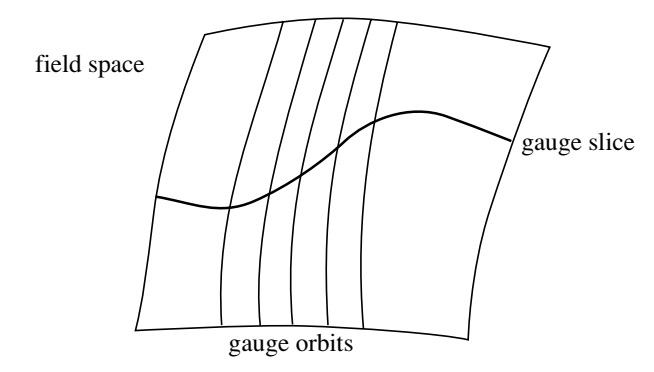
\includegraphics[width=0.8\textwidth]{figure/Fig3.7.jpg}\\
		\caption{Graphical representation of the Faddeev–Popov procedure. A gauge orbit is a family of gauge-equivalent configurations. Integrating over the entire field space and dividing by the orbit volume is equivalent to integrating on a slice that intersects all orbits exactly once.    }\label{Fig:3.7}
	\end{center}
\end{figure}


Let $\zeta$ be the combination of coordinate transformations and Weyl transformations    
\begin{equation}
	\zeta: g \rightarrow g^{\zeta}, \quad g_{a b}^{\zeta}(\sigma^{\prime}) = 
	\exp [2 \omega(\sigma)] \frac{\partial \sigma^{c}}{\partial \sigma^{\prime a}} \frac{\partial \sigma^{d}}{\partial \sigma^{\prime b}} g_{c d}(\sigma) \:.
	\label{3.3.10}
\end{equation}
According to standard procedure, define the Faddeev-Popov measure $\Delta_{\mathrm{FP}}$    
\begin{equation}\label{3.3.11}
	1=\Delta_{\mathrm{FP}}(g) \int[\dif \zeta] \: \delta(g-\hat{g}^{\zeta}) \:, 
\end{equation}
where $\hat{g}_{a b}$ is the fiducial metric. In \eqref{3.3.11}, $[\dif \zeta]$ is the gauge-invariant measure on the diff $\times$ Weyl group. The $\delta$-function is actually a $\delta$-functional, requiring $g_{a b}(\sigma)=\hat{g}_{a b}^{\zeta}(\sigma)$ at every point.    
Substituting \eqref{3.3.11} into the functional integral \eqref{3.3.1}    
\begin{equation}
	Z[\hat{g}]=\int \frac{[\dif \zeta \,\dif X \,\dif g]}{V_{\text {diff } \times \text { Weyl }}}  \Delta_{\mathrm{FP}}(g) \delta(g-\hat{g}^{\zeta}) \exp (-S[X, g]) \:.
	\label{3.3.12}
\end{equation}
Integrating over $g_{ab}$ and renaming the integration variable $X \to X^{\zeta}$ gives    
\begin{equation}
	Z[\hat{g}]=\int \frac{[\dif \zeta\, \dif X^{\zeta}]}{V_{\text {diff } \times \text { Weyl }}} \Delta_{\mathrm{FP}}(\hat{g}^{\zeta}) \exp (-S[X^{\zeta}, \hat{g}^{\zeta}]) \:.
	\label{3.3.13}
\end{equation}
Now, utilizing the gauge invariance of $\Delta_{\mathrm{FP}}$\footnote{Gauge invariance of $\Delta_{\mathrm{FP}}$: 
	\begin{align*}
		\Delta_{\mathrm{FP}}(g^{\zeta})^{-1} &=\int[\dif \zeta^{\prime}] \: \delta(g^{\zeta}-\hat{g}^{\zeta^{\prime}})
		=\int[\dif \zeta^{\prime}]\: \delta(g-\hat{g}^{\zeta^{-1} \cdot \zeta^{\prime}}) \\
		&=\int[\dif \zeta^{\prime \prime}] \: \delta(g-\hat{g}^{\zeta^{\prime \prime}})=\Delta_{\mathrm{FP}}(g)^{-1} \:,
	\end{align*}
	where $\zeta^{\prime \prime}=\zeta^{-1} \cdot \zeta^{\prime} $.}, the invariance of the functional integral measure $[\dif X]$, and the gauge invariance of the action, we get:    
\begin{equation}
	Z[\hat{g}]=\int \frac{[\dif \zeta\, \dif X]}{V_{\text {diff } \times \text { Weyl }}} \Delta_{\mathrm{FP}}(\hat{g}) \exp (-S[X, \hat{g}]) \:.
	\label{3.3.14}
\end{equation}
Finally, since nothing in the integrand depends on $\zeta$, the integral over $\zeta$ merely yields the volume of the gauge group and cancels with the denominator, leaving    
\begin{equation}
	Z[\hat{g}]=\int[\dif X] \: \Delta_{\mathrm{FP}}(\hat{g}) \exp (-S[X, \hat{g}]) \:. \label{3.3.15}
\end{equation}
Thus, $\Delta_{\mathrm{FP}}(\hat{g})$ is the correct measure on the slice.    

To calculate the expression for the Faddeev-Popov measure \eqref{3.3.11}, we assume that the choice of gauge perfectly fixes the gauge symmetry, so that for exactly one value of $\zeta$, $\delta(g-\hat{g} ^\zeta)$ is non-zero; for $\delta(g-\hat{g}^ \zeta)$, this is an equality.    
As mentioned earlier, there is a small global mismatch, which we will address later when time is involved—it does not affect the local properties of the worldsheet. For $\zeta$ near identity, we can expand    
\begin{align}
	\delta g_{a b} &=(1-\mathcal{L}_{\sigma})(1+2\delta\omega)g_{ab}-g_{ab}=2 \delta \omega \,g_{a b}-\nabla_{a} \delta \sigma_{b}-\nabla_{b} \delta \sigma_{a} \nonumber \\
	&=\underbrace{(2 \delta \omega-\nabla_{c} \delta \sigma^{c}) g_{a b}}_{\rm trace \,part}-2(P_{1} \delta \sigma)_{a b} \:.
	\label{3.3.16}
\end{align}
where $P_1$ is the differential operator that takes a vector into a traceless symmetric 2-tensor   
\begin{equation}
	(P_{1} \delta \sigma)_{a b}=\frac{1}{2}(\nabla_{a} \delta \sigma_{b}+\nabla_{b} \delta \sigma_{a}-g_{a b} \nabla_{c} \delta \sigma^{c}) \:.
	\label{3.3.17}
\end{equation}
This is the part of a diffeomorphism that actually changes the shape of the metric, after removing pure scaling. We need this operator because we want to split:
\begin{equation}
	\delta g = \underbrace{\text{Weyl}}_{\text{trace}}+\underbrace{\text{diffeo}}_{\text{pure gauge}} +\underbrace{\text{physical (moduli)}}_{\text{not gauge}}.
\end{equation}
Because of Weyl symmetry of the worldsheet, the first two manifest as pure gauge in String Theory.
\begin{tcolorbox}[breakable]
	\begin{proof}
		We need to work out
		
		\[
		\delta g_{ab}(\sigma) = g'_{ab}(\sigma) - g_{ab}(\sigma) 
		\]
		
		for an infinitesimal version of (3.3.10), i.e. with \( e^{2\omega} = 1 + 2\omega \) and \(\sigma'_a = \sigma_a + \delta\sigma_a\) First, we see that
		
		\[
		\frac{\partial \sigma^a}{\partial \sigma'^b} = \delta^a_b - \partial_b \delta^a 
		\]
		
		Thus, to first order,
		
		\[
		\begin{aligned}
			\delta g_{ab}(\sigma) &= g'_{ab}(\sigma) - g_{ab}(\sigma) = g'_{ab}(\sigma' - \delta\sigma) - g_{ab}(\sigma) =(1-\mathcal{L}_{\sigma})g'_{ab}(\sigma')-g_{ab}(\sigma)\\
			&= g'_{ab}(\sigma') - \delta\sigma^c \partial_c g'_{ab}(\sigma') - g_{ab}(\sigma) \\
			&= (1 + 2\omega)(\delta^c_a - \partial_a \delta^c) (\delta^d_b - \partial_b \delta^d)g_{cd}(\sigma) - \delta^c \partial_c g_{ab}(\sigma') - g_{ab}(\sigma) \\
			&= \delta^c_a \delta^d_b g_{cd} - \delta^d_b \partial_a \delta^c g_{cd} - \delta^c_a \partial_b \delta^d g_{cd} + 2\omega \delta^c_a \delta^d_b g_{cd} - \delta^c \partial_c g_{ab} - g_{ab} \\
			&= 2\omega g_{ab} - \partial_a \delta^c g_{bc} - \partial_b \delta^d g_{ad} - \delta^c \partial_c g_{ab} 
		\end{aligned}
		\]
		
		We now use \(\delta \sigma^a = g^{ab} \delta \sigma_b\):
		
		\[
		\begin{aligned}
			\delta g_{ab}(\sigma) &= 2\omega g_{ab} - \partial_a (g^{cd} \delta \sigma_d) g_{bc} - \partial_b (g^{cd} \delta \sigma_c) g_{ad} - \delta^c \partial_c g_{ab} \\
			&= 2\omega g_{ab} - \partial_a g^{cd} \delta \sigma_d g_{bc} - \partial_a \delta \sigma_d g^{cd} g_{bc} - \partial_b g^{cd} \delta \sigma_c g_{ad} - g^{cd} \partial_b \delta \sigma_c g_{ad} - \delta^c \partial_c g_{ab} \\
			&= 2\omega g_{ab} + \delta \sigma_d g^{cd} \partial_a g_{bc} - \partial_a \delta \sigma_d g^d_b + \delta \sigma_c g^{cd} \partial_b g_{ad} - \partial_b \delta \sigma_c \delta^c_a - \delta^c \partial_c g_{ab} \\
			&= 2\omega g_{ab} - \partial_a \delta \sigma_b - \partial_b \delta \sigma_a + \delta \sigma_d g^{cd} \partial_a g_{bc} + \delta \sigma_c g^{cd} \partial_b g_{ad} - g^{cd} \delta \sigma_d \partial_c g_{ab} \\
			&= 2\omega g_{ab} - \partial_a \delta \sigma_b - \partial_b \delta \sigma_a + \delta \sigma_d g^{cd} (\partial_a g_{bc} + \partial_b g_{ac} - \partial_c g_{ab}) 
		\end{aligned}
		\]
		
		Let us now work out \( \nabla_a \delta \sigma_b + \nabla_b \delta \sigma_a \) keeping in mind that because the indices are downstairs, the connection gets a minus sign
		
		\[
		\begin{aligned}
			\nabla_a \delta \sigma_b + \nabla_b \delta \sigma_a &= \partial_a \delta \sigma_b - \Gamma^c_{ab} \delta \sigma_c + \partial_b \delta \sigma_a - \Gamma^c_{ba} \delta \sigma_c \\
			&= \partial_a \delta \sigma_b + \partial_b \delta \sigma_a - (\Gamma^c_{ab} + \Gamma^c_{ba}) \delta \sigma_c \\
			&= \partial_a \delta \sigma_b + \partial_b \delta \sigma_a - 2 \Gamma^d_{ab} \delta \sigma_d \\
			&= \partial_a \delta \sigma_b + \partial_b \delta \sigma_a - \delta \sigma_d g^{cd} (\partial_a g_{bc} + \partial_b g_{ac} - \partial_c g_{ab})
		\end{aligned}
		\]
		
		and we see that indeed
		
		\[
		\delta g_{ab}(\sigma) = 2 \omega g_{ab} - \nabla_a \delta \sigma_b - \nabla_b \delta \sigma_a
		\]
		
		If we now just fill in the definition of \( P_1 \) in \eqref{3.3.16} we get
		
		\[
		\begin{aligned}
			\delta g_{ab} &= 2 \delta \omega g_{ab} - \nabla_c \delta \sigma^c g_{ab} - (\nabla_a \delta \sigma_b + \nabla_b \delta \sigma_a - g_{ab} \nabla_c \delta \sigma^c) \\
			&= 2 \delta \omega g_{ab} - \nabla_a \delta \sigma_b - \nabla_b \delta \sigma_a
		\end{aligned}
		\]
		
		Which shows that the first and second line of \eqref{3.3.16} are equal.	Next, we show that \( P_1 \) takes vectors into traceless symmetric tensors. First, it is obvious from the definition \eqref{3.3.17} that
		
		\[
		(P_1 \delta \sigma)_{ab} = (P_1 \delta \sigma)_{ba}
		\]
		
		Next, also the tracelessness is obvious
		
		\[
		\begin{aligned}
			g^{ab}(P_1 \delta \sigma)_{ab} &= g^{ab} \frac{1}{2} (\nabla_a \delta \sigma_b + \nabla_b \delta \sigma_a - g_{ab} \nabla_c \delta \sigma^c) \\
			&= \frac{1}{2} (2 \nabla_a \delta \sigma^a - \delta^a_a \nabla_c \delta \sigma^c) = 0
		\end{aligned}
		\]
		
		But notice that the tracelessness is only valid in two dimensions.
	\end{proof}
\end{tcolorbox}
Near identity, the inverse determinant \eqref{3.3.11} becomes    
\begin{align}
	\Delta_{\mathrm{FP}}(\hat{g})^{-1}	&\quad =\int[\dif \delta \omega \, \dif \delta \sigma]\: \delta\bigl[g-g^{\zeta}\bigr]=\int[\dif \delta \omega \, \dif \delta \sigma]\: \delta\big[-\delta g\big] \nonumber \\	
	&\quad =\int[\dif \delta \omega \, \dif \delta \sigma]\: \delta\Bigl[-(2 \delta \omega-\hat{\nabla} \cdot \delta \sigma) \hat{g}+2 \hat{P}_{1} \delta \sigma\Bigr] \nonumber \\
	&\quad =\int[\dif \delta \omega \, \dif \beta\, \dif \delta \sigma] \: \exp \biggl\{2 \pi \mi \int \dif^{2} \sigma \: \hat{g}^{1 / 2} \beta^{a b}
	\Bigl[-(2 \delta \omega-\hat{\nabla} \cdot \delta \sigma) \hat{g}+2 \hat{P}_{1} \delta \sigma\Bigr]_{a b}\biggr\} \nonumber \\
	&\quad =\int[\dif \beta^{\prime}\, \dif \delta \sigma]\: \exp \biggl\{4 \pi \mi \int \dif^{2} \sigma \: \hat{g}^{1 / 2} \beta^{\prime a b}
	(\hat{P}_{1} \delta \sigma)_{a b}\biggr\} \:.
	\label{3.3.18}
\end{align}
The hat on the differential operator indicates that it contains the fiducial metric $\hat{g}$. In the second equality, we used the integral representation of the functional $\delta$-function, introducing the symmetric tensor field $\beta^{a b} $. 
In the fourth equality, we integrated out $\delta \omega$, which produced a $\delta$-functional forcing $\beta^{a b}$ to be traceless; 
\begin{equation}
	\int [d\delta\omega]\,
	\exp\left(
	-4\pi i \int d^2\sigma \sqrt{\hat g}\, \beta^{ab} \hat g_{ab}\, \delta\omega
	\right)
	= \frac{1}{2\pi} \delta\!\left(4\pi \beta^{ab} \hat g_{ab}\right)
	\tag{3.34}
\end{equation}
then the functional integral $[\dif \beta^{\prime}]$ is over \emph{traceless} symmetric tensors.    
We now have an expression for $\Delta_{\mathrm{FP}}(\hat{g})^{-1}$ as a functional integral over the vector field $\delta \sigma^{a}$ and the traceless symmetric tensor $\beta^{\prime a b}$.    

By replacing the bosonic fields with corresponding Grassmann \emph{ghost} fields    
\begin{subequations} \label{3.3.19}
	\begin{align}
		\delta \sigma^{a} &\rightarrow c^{a} \:, \label{3.3.19a}\\
		\beta_{a b}^{\prime} & \rightarrow b_{a b} \:, \label{3.3.19b}
	\end{align}
\end{subequations}
we can transform the path integral, where $b^{a b}$ is traceless like $\beta^{\prime a b}$.    
Hence,    
\begin{equation}
	\Delta_{\mathrm{FP}}(\hat{g})=\int[\dif b\, \dif c] \: \exp (-S_{\mathrm{g}}) \:, \label{3.3.20}
\end{equation}
where, under a convenient normalization of the fields, the ghost action is    
\begin{equation}\label{3.3.21}
	S_{\mathrm{g}}=\frac{1}{2 \pi} \int \dif^{2} \sigma \: \hat{g}^{1 / 2} b_{a b} \hat{\nabla}^{a} c^{b}=\frac{1}{2 \pi} \int \dif^{2} \sigma \hat{g}^{1 / 2} b_{a b}(\hat{P}_{1}, c)^{a b} \:.
\end{equation}
Locally on the worldsheet, the Polyakov path integral is    
\begin{equation}\label{3.3.22}
	Z[\hat{g}]=\int[\dif X\, \dif b\, \dif c]\: \exp (-S_{X}-S_{\mathrm{g}}) \:. 
\end{equation}
Since this action is quadratic in the fields, we can express the path integral in the form of determinants. This calculation will be described in more detail in Chapter \ref{cha:5};    
the result is    
\begin{equation}
	Z[\hat{g}]=(\operatorname{det} \hat{\nabla}^{2})^{-D / 2} \operatorname{det} \hat{P}_{1} \:, \label{3.3.23}
\end{equation}
where the first determinant comes from the $X$ integration and the second from the ghost integration.    

In the conformal gauge, $\hat{g}_{a b}(\sigma)=\exp [2 \omega(\sigma)] \delta_{a b}$, the ghost action \eqref{3.3.21} is    
\begin{align}
	S_{\mathrm{g}} &=\frac{1}{2 \pi} \int \dif^{2} z\:\Bigl(b_{z z} \nabla_{\bar{z}} c^{z}+b_{\bar{z} \bar{z}} \nabla_{z} c^{\bar{z}}\Bigr)  \nonumber \\
	&=\frac{1}{2 \pi} \int \dif^{2} z\:\Bigl(b_{z z} \partial_{\bar{z}} c^{z}+b_{\bar{z} \bar{z}} \partial_{z} c^{\bar{z}}\Bigr) \:.
	\label{3.3.24}
\end{align}
Note that $\omega(\sigma)$ does not appear in the final form. This is because if a tensor has only $z$ indices, its covariant $\bar{z}$ derivative simplifies to a simple derivative, and vice-versa, which the reader can verify by solving for the connection tensor. 
Since the action \eqref{3.3.24} is Weyl invariant, $b_{a b}$ and $c^{a}$ are neutral under local Weyl transformations (while $b^{a b}$ and $c_{a}$ are not; they contain extra metric factors).    
Because a conformal transformation is a combination of a coordinate transformation \eqref{3.3.7} and a Weyl transformation \eqref{3.3.9}, we can immediately read off the conformal transformations of $b_{a b}$ and $c^{a}$ from the tensor indices: these are the $bc$ CFT with $(h_{b}, h_{c})=(2,-1)$ and the $\tilde{b} \tilde{c}$ CFT with $(\tilde{h}_{b}, \tilde{h}_{c})=(2,-1)$.    

The method we used to derive the gauge-fixed path integral is sometimes called a "heuristic" derivation. The Polyakov functional integral \eqref{3.3.1} is not reasonably defined due to massive gauge overcounting.    
On the other hand, the gauge-fixed functional \eqref{3.3.22} is quite well defined and can be calculated clearly. For practical reasons, we should perhaps regard the gauge-fixed form as the starting point, while the gauge-invariant one gives a direct interpretation. In the gauge-fixed form, the substance of gauge symmetry is expressed as BRST invariance, which we will address in the next chapter.    

For open strings, we must also consider parts containing boundary segments. It is convenient to view the functional integral as an integral of fields over a fixed region, so diff invariance is restricted to coordinate transformations that map boundaries to themselves. Thus, the variation $\delta \sigma^{a}$ has a zero normal component    
\begin{equation}
	n_{a} \delta \sigma^{a}=0 \:. \label{3.3.25}
\end{equation}
This boundary condition is inherited by the corresponding ghost field    
\begin{equation}
	n_{a} c^{a}=0 \:, \label{3.3.26}
\end{equation}
so $c^{a}$ is proportional to the tangent vector $t^{a}$. Then the equations of motion provide a boundary condition for $b_{a b}$. They have surface terms    
\begin{equation}
	\int_{\partial M} \dif s\: n^{a} b_{a b} \delta c^{b}=0 \:. \label{3.3.27}
\end{equation}
Combining with the boundary condition on $c^a$,    
this implies    
\begin{equation}
	n_{a} t_{b} b^{a b}=0 \:. \label{3.3.28}
\end{equation}
These are the boundary conditions used in Section \ref{sec:2.7}.    

\section{\texorpdfstring{The Weyl anomaly}{3.4 The Weyl anomaly}} \label{sec:3.4}

A key feature of string theory is that it is self-consistent only in specific spacetime backgrounds. For bosonic string theory in flat spacetime, the condition is $D=26$. It was first discovered from a pathology in scattering amplitudes. In light-cone analysis, it originated from the loss of Lorentz symmetry. The underlying cause of this constraint is an \emph{anomaly} in local worldsheet symmetry.    
In our current formalism, the anomaly is in the Weyl symmetry: $T^{a}{}_{a}$ is zero in the classical sense, but not in the quantum theory.    

A global Weyl transformation, $\omega(\sigma)=$ constant, is equivalent to a general scaling of length. Several field theories in four dimensions are invariant under such a scaling. These include the $\phi^4$ massless scalar field theory and non-Abelian gauge field theories. Scale invariance is apparent because the Lagrangian contains only dimensionless parameters—the coupling constant in each case is dimensionless. However, due to divergences in quantum theory, there is a non-zero renormalization group $\beta$ function in each theory, implying that the effective coupling constant is actually a function of the length scale.    
Correspondingly, the trace of the energy-momentum tensor is zero in the classical theory, but after quantum effects are considered, the trace is non-zero and proportional to the $\beta$ function.    

In the previous section, we ignored the possibility of anomalies. We need to verify whether the gauge-fixed path integral $Z[g]$ is truly independent of the choice of fiducial metric,    
\begin{equation}
	Z[g^{\zeta}]=Z[g]\:? \label{3.4.1}
\end{equation}
In Section \ref{sec:4.2}, we will generalize this to more general gauge transformations. For convenience, hereafter $g$ without a hat denotes the fiducial metric.    
We are also interested in path integrals with extra insertions    
\begin{equation}
	\langle\mathcal{O}\rangle_{g} \equiv \int[\dif X\, \dif b \, \dif c] \:e^{-S[X, b, c, g]} \mathcal{O} \:. \label{3.4.2}
\end{equation}
Then, we require    
\begin{equation}
	\langle\mathcal{O}\rangle_{g ^\zeta}=\langle\mathcal{O}\rangle_{g} \:. \label{3.4.3}
\end{equation}
Currently, we are not interested in the details of the insertions—that will be the subject of the next two sections—we restrict our attention to gauge transformations where $\zeta$ is zero near the field positions in "$\mathcal{O}$". That is, we want to know if Weyl invariance holds as an operator equation.    

It is easy to guarantee diff invariance and Poincaré invariance in quantum theory. For example, the gauge-fixed path integral can be defined using Pauli-Villars regularization, dividing the path integral by a massive regulator field. A massive regulator field can be coupled to the metric in a diff-invariant and Poincaré-invariant way. However, for a regulator field $Y^\mu$, the diff-invariant and Poincaré-invariant term $\mu^{2}\int \dif^{2} \sigma\: g^{1/2} Y^{\mu} Y_{\mu}$ is not Weyl-invariant. Any Weyl transformation can be obtained by repeated infinitesimal transformations, so studying infinitesimal transformations is sufficient.    
The energy-momentum tensor $T^{\mu\nu}$ is the infinitesimal variation of the path integral with respect to the metric,    
\begin{equation}\label{3.4.4}
	\delta\langle\mathcal{O}\rangle_{g}=-\frac{1}{4 \pi} \int \dif^{2} \sigma \: g(\sigma)^{1 / 2} \delta g_{a b}(\sigma)\Bigl\langle T^{a b}(\sigma) \mathcal{O}\Bigr\rangle_{g}
\end{equation}
Classically, $T^{\mu\nu}$ originates entirely from the variation of the action, and this is consistent with the Noether definition    
\begin{equation}
	T^{a b}(\sigma) \stackrel{\text { classical }}{=} \frac{4 \pi}{g(\sigma)^{1 / 2}} \frac{\delta}{\delta g_{a b}(\sigma)} S \:. \label{3.4.5}
\end{equation}
In the flat worldsheet limit, it also reduces to the earlier definition. If we take $\delta g_{a b}$ to have the form of a coordinate transformation, the diff invariance of the path integral implies that $T^{ab}$ is conserved.    

In the following analysis, we will first ignore possible boundary terms. For a Weyl transformation, the definition of $T^{ab}$ in \eqref{3.4.4} implies    
\begin{equation}\label{3.4.6}
	\delta_{\mathrm{W}}\langle\cdots\rangle_{g}=-\frac{1}{2 \pi} \int \dif^{2} \sigma\: g(\sigma)^{1 / 2} \delta \omega(\sigma)\langle T^{a}{}_{a}(\sigma) \cdots\rangle_{g} \:,
\end{equation}
\begin{tcolorbox}
	\begin{proof}
		Use $\delta g_{ab}=2\omega g_{ab}$ in \eqref{3.4.4}.
	\end{proof}
\end{tcolorbox}
so for general insertions "$\dots$", Weyl invariance can be stated as an operator statement: the energy-momentum tensor is traceless    
\begin{equation}
	{T^a}_{a} \stackrel{?}{=} 0 \:. \label{3.4.7}
\end{equation}
The classical action is Weyl invariant, but in the quantum theory, since we haven't found a completely gauge-invariant regulator, this trace might be non-zero. This trace must be diff invariant and Weyl invariant because we protected these symmetries; it is zero on a flat worldsheet because we know from the previous chapter that the theory is conformally flat. This leaves only one possibility:    
\begin{equation}\label{3.4.8}
	T^{a}{}_{a}=a_{1} R \:,
\end{equation}
where $a_1$ is some constant and $R$ is the worldsheet Ricci scalar. Terms with two or more derivatives are forbidden for dimensional reasons. When using worldsheet length as the unit, $g_{ab}$ and $X^\mu$ are dimensionless, so the constant $a_1$ in \eqref{3.4.8} is also dimensionless.    
Terms with multiple derivatives would have a coefficient with a positive power of the cutoff length scale used to define the path integral, and thus vanish in the limit as the cutoff is taken to zero.    

\subsection*{Calculation of the Weyl anomaly}

The possible obstacle to constructing a gauge-invariant theory has reduced to a single constant $a_1$. In fact, this number is proportional to a quantity we have calculated—the \emph{central charge} $c$ of the CFT on a flat worldsheet. Both $a_1$ and $c$ are related to the two-point function of the energy-momentum tensor, though through different components. To get the precise relationship between them, we will need to use diff invariance.    

In complex coordinates,    
\begin{equation}
	T_{z \bar{z}}=\frac{a_{1}}{2} g_{z \bar{z}} R \:. \label{3.4.9}
\end{equation}
Taking the covariant derivative,    
\begin{equation}
	\nabla^{\bar{z}} T_{\bar{z} z}=\frac{a_{1}}{2} \nabla^{\bar{z}}(g_{z \bar{z}} R)=\frac{a_{1}}{2} \nabla_{z} R=\frac{a_{1}}{2} \partial_{z} R \:, \label{3.4.10}
 \end{equation}
where we used the property that the metric is covariant constant. Then, through the conservation of $T_{ab}$,    
\begin{equation}\label{3.4.11}
	\nabla^{z} T_{z z}=-\nabla^{\bar{z}} T_{\bar{z} z}=-\frac{a_{1}}{2} \partial_{z} R \:.
\end{equation}
To fix $a_1$, we compare the Weyl transformations on both sides.    
The Weyl transformation of the right side, \eqref{3.3.5}, is    
\begin{equation}\label{3.4.12}
	a_{1} \partial_{z} \nabla^{2} \delta \omega \approx 4 a_{1} \partial_{z}^{2} \partial_{\bar{z}} \delta \omega \:,
\end{equation}
where we expand near a flat worldsheet. To get the Weyl transformation on $T_{zz}$, we first use the conformal transformation \eqref{2.4.24},    
\begin{equation}
	\epsilon^{-1} \delta T_{z z}(z)=-\frac{c}{12} \partial_{z}^{3} v^{z}(z)-2 \partial_{z} v^{z}(z) T_{z z}(z)-v^{z}(z) \partial_{z} T_{z z}(z) \:. \label{3.4.13}
\end{equation}
From the discussion in Section \ref{sec:3.3}, this conformal transformation consists of a coordinate transformation $\delta z=\epsilon v$ and a Weyl transformation $2 \delta \omega=\epsilon \partial v+\epsilon(\partial v)^{*}$.    
The last two terms in the variation are coordinate transformations of tensors, so to leading order in flat space, the Weyl transformation is    
\begin{equation}
	\delta_{\mathrm{W}} T_{z z}=-\frac{c}{6} \partial_{z}^{2} \delta \omega \:. \label{3.4.14}
\end{equation}
Acting with $\partial^{z}=2 \partial_{\bar{z}}$ and comparing with the transformation \eqref{3.4.12} gives:    
\begin{equation}
	c=-12 a_{1}, \qquad {T^a}_{a}=-\frac{c}{12} R \:. \label{3.4.15}
\end{equation}
\begin{tcolorbox}[breakable]
	\begin{proof}
		The Weyl anomaly is due to the fact that it is not possible to find a regularization scheme that preserves Weyl invariance. This means that the path integral is not invariant under Weyl transformation. Starting from
		\begin{equation}
			\sqrt{g'} R' = \sqrt{g}(R - 2\nabla^2\omega)
		\end{equation}
		
		For an infinitesimal Weyl transformation \( g'_{ab}(\sigma') = e^{2\delta\omega} g_{ab}(\sigma) = (1 + 2\delta\omega)g_{ab}(\sigma) \) we have for the RHS of \eqref{3.4.11}
		
		\begin{equation}
			\delta_W \nabla^{\bar{z}} T_{\bar{z} z} = -\frac{a_1}{2}\partial_z \delta_W R
		\end{equation}
		
		now
		
		\begin{equation}
			\begin{aligned}
				\delta_W R &= R'(\sigma) - R(\sigma) = \sqrt{\frac{g}{g'}}(R - 2\nabla^2\omega) - R \\
				&= e^{-2\omega}(R - 2\nabla^2\omega) - R = (1 - 2\delta\omega)(R - 2\nabla^2\delta\omega) - R \\
				&= -2\delta\omega R - 2\nabla^2\delta\omega
			\end{aligned}
		\end{equation}
		
		Therefore
		
		\begin{equation}
			\delta_W \nabla^{\bar{z}} T_{\bar{z} z} = -\frac{a_1}{2}\partial_z(-2\delta\omega R - 2\nabla^2\delta\omega)
		\end{equation}
		
		We now expand this near a flat worldsheet, where we have \( R = 0 \) and \( \nabla^2 = 2g^{z\bar{z}}\nabla_z\nabla_{\bar{z}} = 4\partial_z\partial_{\bar{z}} \). This gives
		
		\begin{equation}
			\delta_W \nabla^{\bar{z}} T_{\bar{z} z} = -\frac{a_1}{2}\partial_z(-2 \times 4\partial_z\partial_{\bar{z}}\delta\omega) = 4a_1\partial_z^2\partial_{\bar{z}}\delta\omega
		\end{equation}
		
		Combining \eqref{3.4.12} and \eqref{3.4.14} we find
		
		\begin{equation}
			4a_1 \partial_z^2 \partial_{\bar{z}} \delta \omega = \nabla^z \left( -\frac{c}{6} \partial_z^2 \delta \omega \right) = -\frac{c}{6} g^{z\bar{z}} \partial_z \partial_{\bar{z}} \delta \omega = -\frac{c}{3} \partial_{\bar{z}} \partial_z^2 \delta \omega
		\end{equation}
		
		and so
		
		\begin{equation}
			a_1 = -\frac{c}{12}
		\end{equation}
	\end{proof}
\end{tcolorbox}
We re-derive this once more with a slightly longer procedure, in which we will obtain a useful intermediate result.    
In the conformal gauge,    
\begin{subequations}\label{3.4.16}
	\begin{align}
		R&=-2 \exp (-2 \omega) \partial_{a} \partial_{a} \omega \:,\label{3.4.16a}\\
		\nabla^{2}&=\exp (-2 \omega) \partial_{a} \partial_{a} \:. \label{3.4.16b}
	\end{align}
\end{subequations}
By contracting two lower indices, i.e., $\delta^{a b} \partial_{a} \partial_{b}$.    
The Weyl variation of $Z[g]$, \eqref{3.4.6}, becomes    
\begin{equation}
	\delta_{\mathrm{W}} Z[\exp (2 \omega) \delta]=\frac{a_{1}}{\pi} Z[\exp (2 \omega) \delta] \int \dif^{2} \sigma\: \delta \omega \partial_{a} \partial_{a} \omega \:, \label{3.4.17}
\end{equation}
where $\exp (2 \omega) \delta$ represents the conformal gauge.    
Integration immediately yields    
\begin{equation}\label{3.4.18}
	Z[\exp (2 \omega) \delta]=Z[\delta] \exp \left(-\frac{a_{1}}{2 \pi} \int \dif^{2} \sigma \: \partial_{a} \omega \partial_{a} \omega\right) \:.
\end{equation}
Since every metric is diffeomorphic to a conformal metric, \eqref{3.4.18} actually determines the entire dependence of $Z[g]$ on the metric. We need to find a diff-invariant expression that can reduce to \eqref{3.4.18} in the conformal gauge.    
Utilizing \eqref{3.4.16}, we can prove the expected expression:    
\begin{equation}\label{3.4.19}
	Z[g]=Z[\delta] \exp \left[\frac{a_{1}}{8 \pi} \int \dif^{2} \sigma \int \dif^{2} \sigma^{\prime} \: g^{1 / 2} R(\sigma) G(\sigma, \sigma^{\prime}) g^{1 / 2} R(\sigma^{\prime})\right] \:,
\end{equation}
where the scalar Green's function is defined by    
\begin{equation}
	g(\sigma)^{1 / 2} \nabla^{2} G(\sigma, \sigma^{\prime})=\delta^{2}(\sigma-\sigma^{\prime}) \label{3.4.20}
\end{equation}
This is an interesting result: the path integral is completely determined by the anomaly equation.    
\begin{tcolorbox}[breakable]
	\begin{proof}
		Let us check that \eqref{3.4.19} reduces to \eqref{3.4.18} in the conformal gauge
		
		\begin{equation}
			Z[g] \bigg|_{g=e^{2\omega} \delta_+} = Z[\delta_+] \exp \left\{ \frac{a_1}{8\pi} \int d^2\sigma \int d^2\sigma' e^{2\omega(\sigma)} \left[ -2e^{-2\omega(\sigma)}\partial_a \partial_a \omega(\sigma) \right] \right\}
		\end{equation}
		
		\begin{equation}
			\times G(\sigma, \sigma') e^{2\omega(\sigma')} \left[ -2e^{-2\omega(\sigma')} \partial'_a \partial'_a \omega(\sigma') \right]
		\end{equation}
		
		\begin{equation}
			= Z[\delta_+] \exp \left[ \frac{a_1}{2\pi} \int d^2\sigma \int d^2\sigma' \partial_a \partial_a \omega(\sigma) G(\sigma, \sigma') \partial'_a \partial'_a \omega(\sigma') \right]
		\end{equation}
		
		\begin{equation}
			= Z[\delta_+] \exp \left[ \frac{a_1}{2\pi} \int d^2\sigma \int d^2\sigma' \omega(\sigma) \partial_a \partial_a G(\sigma, \sigma') \partial'_a \partial'_a \omega(\sigma') \right]
		\end{equation}
		
		where we have used partial integration in the last line. We now use \eqref{3.4.16b} and \eqref{3.4.20} to rewrite
		
		\begin{equation}
			\partial_a \partial_a G(\sigma, \sigma') = e^{2\omega} \nabla^2 G(\sigma, \sigma') = e^{2\omega} g^{-1/2} \delta^2(\sigma - \sigma')
		\end{equation}
		
		\begin{equation}
			= e^{2\omega} e^{-2\omega} \delta^2(\sigma - \sigma') = \delta^2(\sigma - \sigma')
		\end{equation}
		
		Thus
		
		\begin{equation}
			Z[g] \bigg|_{g=e^{2\omega} \delta_+} = Z[\delta_+] \exp \left[ \frac{a_1}{2\pi} \int d^2\sigma \, \int d^2\sigma' \, \omega(\sigma) \delta^2(\sigma - \sigma') \partial_a \partial_a' \omega(\sigma') \right]
		\end{equation}
		
		\begin{equation}
			= Z[\delta_+] \exp \left[ \frac{a_1}{2\pi} \int d^2\sigma \, \omega(\sigma) \partial_a \partial_a \omega(\sigma) \right]
		\end{equation}
		
		\begin{equation}
			= Z[\delta_+] \exp \left[ -\frac{a_1}{2\pi} \int d^2\sigma \, \partial_a \omega(\sigma) \partial_a \omega(\sigma) \right]
		\end{equation}
		
		where we have, once more, used partial integration in the last line. Note also that \eqref{3.4.19} is manifestly diffeomorphism invariant. Indeed \( R \) and \( G \) are scalar functions and the measure in the integrals is the diffeomorphism invariant measure \( d^2\sigma \sqrt{g} \).
	\end{proof}
\end{tcolorbox}

Now expand $Z[g]$ around a flat background, $g_{a b}=\delta_{a b}+h_{a b}$, and retain terms up to second order in $h_{\bar{z} \bar{z}} $.    
To first order in $h_{\bar{z} \bar{z}}$, the Ricci scalar is $4 \partial_{z}^{2} h_{\bar{z} \bar{z}}$, so    
\begin{align}
	\ln \frac{Z[\delta+h]}{Z[\delta]} & \approx \frac{a_{1}}{8 \pi^{2}} \int \dif^{2} z \int \dif^{2} z^{\prime} \:
	(\partial_{z}^{2} \ln \lvert z-z^{\prime}\rvert^{2}) h_{\bar{z} \bar{z}}(z, \bar{z}) \partial_{z^{\prime}}^{2} h_{\bar{z} \bar{z}}(z^{\prime}, \bar{z}^{\prime}) \nonumber \\
	&=-\frac{3 a_{1}}{4 \pi^{2}} \int \dif^{2} z \int \dif^{2} z^{\prime} \: \frac{h_{\bar{z} \bar{z}}(z, \bar{z}) h_{\bar{z} \bar{z}}(z^{\prime}, \bar{z}^{\prime})}{(z-z^{\prime})^{4}} \:. \label{3.4.21}
\end{align}
We can calculate it using second-order perturbation theory in the metric, which is given by \eqref{3.4.4}:    
\begin{equation}
	\ln \frac{Z[\delta+h]}{Z[\delta]} \approx \frac{1}{8 \pi^{2}} \int \dif^{2} z \int \dif^{2} z^{\prime} \: h_{\bar{z} \bar{z}}(z, \bar{z}) h_{\bar{z} \bar{z}}(z^{\prime}, \bar{z}^{\prime})\bigl\langle T_{z z}(z) T_{z z}(z^{\prime})\bigr\rangle_{\delta} \:. \label{3.4.22}
\end{equation}
Now use the standard $TT$ OPE \eqref{2.4.25}. Except for the first term containing a non-zero spin operator, all terms are zero due to rotational invariance, leaving $\bigl\langle T_{z z}(z) T_{z z}(z^{\prime})\bigr\rangle_{1}=\frac{1}{2} c(z-z^{\prime})^{-4}$. Comparing with the result \eqref{3.4.21} from the Weyl anomaly gives \eqref{3.4.15} once again.    
\begin{tcolorbox}[breakable]
	\begin{proof}
		We first compute the Ricci scalar in the linear limit. If \( g_{ab} = \delta_{ab} + h_{ab} \) then in complex coordinates we need a linear deformation from \( g_{zz} = g_{\bar{z}\bar{z}} = 0 \) and \( g_{z\bar{z}} = 1/2 \). Thus
		
		\begin{equation}
			g_{ab} = 
			\begin{pmatrix}
				h_{zz} & \frac{1}{2} + h_{z\bar{z}} \\
				\frac{1}{2} + h_{z\bar{z}} & h_{\bar{z}\bar{z}}
			\end{pmatrix}
		\end{equation}
		
		The inverse metric is
		
		\begin{equation}
			g^{ab} = 
			\begin{pmatrix}
				-4h_{z\bar{z}} & 2(1 - 2h_{z\bar{z}}) \\
				2(1 - 2h_{z\bar{z}}) & -4h_{zz}
			\end{pmatrix}
		\end{equation}
		
		This is easily checked by multiplying the two matrices with one another and showing that they are equal to the identity matrix plus terms of second order in \( h \). To calculate the determinant \( \sqrt{g} \) we first revert to the ordinary worldsheet coordinates. We have
		
		\begin{equation}
			\begin{aligned}
				ds^2 &= g_{zz} dz \, dz + g_{\bar{z}\bar{z}} d\bar{z} \, d\bar{z} + 2g_{z\bar{z}} dz \, d\bar{z} \\
				&= h_{zz}(d\sigma^1 + id\sigma^2)^2 + h_{\bar{z}\bar{z}}(d\sigma^1 - id\sigma^2)^2 + (1 + 2h_{z\bar{z}}(d\sigma^1 + id\sigma^2))(d\sigma^1 - id\sigma^2) \\
				&= (1 + h_{zz} + h_{\bar{z}\bar{z}} + 2h_{z\bar{z}})d\sigma^1 d\sigma^1 + (1 - h_{zz} - h_{\bar{z}\bar{z}} + 2h_{z\bar{z}})d\sigma^2 d\sigma^2 \\
				&\quad + 2i(h_{zz} - h_{\bar{z}\bar{z}})d\sigma^1 d\sigma^2
			\end{aligned}
		\end{equation}
		
		and therefore
		
		\begin{align}
			g_{11} &= 1 + h_{zz} + h_{\bar{z}\bar{z}} + 2h_{z\bar{z}} \\
			g_{22} &= 1 - h_{zz} - h_{\bar{z}\bar{z}} + 2h_{z\bar{z}} \\
			g_{12} &= i(h_{zz} - h_{\bar{z}\bar{z}})
		\end{align}
		
		The determinant is therefore
		
		\begin{equation}
			\begin{aligned}
				g &= (1 + h_{zz} + h_{\bar{z}\bar{z}} + 2h_{z\bar{z}})(1 - h_{zz} - h_{\bar{z}\bar{z}} + 2h_{z\bar{z}}) + (h_{zz} - h_{\bar{z}\bar{z}})^2 \\
				&= 1 + 4h_{zz} + o(h^2)
			\end{aligned}
		\end{equation}
		
		and
		
		\begin{equation}
			\sqrt{g} = 1 + 2h_{zz} + o(h^2)
		\end{equation}
		The calculation of \( R \) is rather messy, so it was evaluated using mathematica, focussing on the linear terms, the result is quite simple
		
		\begin{equation}
			R = 4\partial_{\bar z}^2 h_{zz} + 4\partial_z^2 h_{\bar{z}\bar{z}} - 8\partial_z \partial_{\bar{z}} h_{z\bar{z}} + o(h^2)
		\end{equation}
		We now focus on the terms with \( h_{\bar z\bar{z}} \) only. This means that to first order we can take \(\sqrt{g} = 1\) and \( R = 4\partial_z^2 h_{\bar z\bar z} \). Moreover the solution of \eqref{3.4.20} is something we already know; it is given by \eqref{2.1.24}, i.e. \( \partial\bar{\partial} \ln |z|^2 = 2\pi\delta^2(z,\bar{z}) \). Using \( \nabla^2 = 2\partial\bar{\partial} + o(h) \) we get
		
		\begin{equation}
			G(\sigma, \sigma') = \frac{1}{4\pi} \ln |z - z'|^2
		\end{equation}
		
		We can now use all this in \eqref{3.4.19}:
		
		\begin{equation}
			\begin{aligned}
				Z[g] &= Z[\delta] \exp \frac{a_1}{8\pi} \int \frac{1}{2} d^2 z \int \frac{1}{2} d^2 z' \times 1 \times 4\partial_z^2 h_{\bar z\bar{z}}(z,\bar{z}) \times \frac{1}{4\pi} \ln |z - z'|^2 \times 1 \times 4\partial_z^2 h_{\bar{z}\bar{z}}(z',\bar{z}') \\
				&= Z[\delta] \exp \frac{a_1}{8\pi^2} \int d^2 z \int d^2 z' \partial_z^2 h_{\bar z\bar{z}}(z,\bar{z}) \ln |z - z'|^2 \partial_z^2 h_{\bar{z}\bar{z}}(z',\bar{z}')
			\end{aligned}
		\end{equation}
		
		Using partial integration and \( g = \delta + h \) this gives
		
		\begin{equation}
			\ln \frac{Z[\delta + h]}{Z[\delta]} = \frac{a_1}{8\pi^2} \int d^2 z \int d^2 z' h_{\bar z\bar{z}}(z,\bar{z}) \partial_z^2 \partial_z^2 (\ln |z - z'|^2) h_{\bar{z}\bar{z}}(z',\bar{z}')
		\end{equation}
		
		Now \( \partial_z^2 \partial_z^2 \ln |z - z'|^2 = -6/(z - z')^4 \) so that we find \eqref{3.4.21}.
		
		\begin{equation}
			\ln \frac{Z[\delta + h]}{Z[\delta]} = -\frac{3a_1}{4\pi^2} \int d^2 z \int d^2 z' \frac{h_{\bar z\bar{z}}(z,\bar{z}) h_{\bar{z}\bar{z}}(z',\bar{z}')}{(z-z')^4}
		\end{equation}
	\end{proof}
\end{tcolorbox}
\subsection*{Discussion}
For a worldsheet theory consisting of $X^\mu$ with central charge $D$ and ghosts with central charge $-26$, the total central charge is    
\begin{equation}
	c=c^{X}+c^{g}=D-26 \:, \label{3.4.23}
\end{equation}
where the ghost central charge is given by \eqref{2.5.12} with $\lambda=2$. This theory is Weyl invariant only for $D=26$, the same condition for Lorentz invariance found in Chapter 1.    
When the Weyl anomaly is non-zero, different gauge choices are not equivalent, and just as in gauge theories with anomalies, any one choice leads to an inconsistency, such as loss of covariance or unitarity. For example, in the light-cone gauge, choosing a different spacetime background would require a specific gauge range, thus transforming the potential Weyl anomaly into a Lorentz anomaly.    

There is another thing to try: ignore the Weyl anomaly and only treat diff invariance as gauge symmetry. Then the metric will have a real degree of freedom $\omega(\sigma)$ that must be integrated out instead of being gauge-fixed. Since the quantum effects in \eqref{3.4.18} act on $\omega$ like an action for an $X^\mu$; when $D<26$, this sign is spacelike. However, the physics is a bit strange, because the diff transformations of $\omega$ and the subsequent energy-momentum tensor are different from those of $X^\mu$.    
In fact, this theory is a linear dilaton CFT. Thus, there is no $D+1$ dimensional Lorentz invariance, and this theory is useless for our current purposes, namely understanding physics as part of our universe. It is an interesting model, and we will return to it briefly in Section 9.9.    

Above, we found that a flat worldsheet CFT can couple to a curved metric in a Weyl-invariant way if and only if the total central charge $c$ is zero. However, there is a contradiction, since the same discussion applies to the anti-holomorphic central charge $\tilde{c}$, and we have seen from the example of $bc$ CFT that $c$ does not need to equal $\tilde{c}$. The key point is that in \eqref{3.4.11} and \eqref{3.4.19}, we implicitly assumed worldsheet diff invariance.    
If $c\neq \tilde{c}$, then no diff-invariant expression exists that is consistent with both $O(h_{z z}^{2})$ and $O(h_{\bar{z} \bar{z}}^{2})$ calculations, so the CFT \emph{cannot} couple to a curved metric in a diff-invariant way; there is a \emph{diff} anomaly or \emph{gravitational} anomaly.    
The contradiction indicates that $c= \tilde{c}$ is necessary for a CFT to be free of gravitational anomalies, and it can be proven to be sufficient.    

\subsection*{Introducing boundaries}

First, return to equation \eqref{3.4.8} and consider a more general possibility    
\begin{equation}\label{3.4.24}
	T^{a}{}_{a}=a_{1} R+a_{2} \:. 
\end{equation}
This is allowed by diff invariance but is non-zero in the flat limit.    
Earlier we set $a_2=0$ through the choice of $T_{ab}$ in \eqref{2.3.15b}. Equivalently, having more than one conserved $T_{ab}$ on a flat worldsheet means there is freedom in how to couple to a curved metric.    
Specifically, we can add the action    
\begin{equation}
	S_{\mathrm{ct}}=b \int \dif^{2} \sigma \: g^{1 / 2} \:, \label{3.4.25}
\end{equation}
which is a two-dimensional cosmological constant and is not Weyl invariant.    
It adds $2 \pi b g_{a b}$ to $T_{ab}$, so the trace \eqref{3.4.24} becomes    
\begin{equation}
	T^{a}{}_{a}=a_{1} R+\left(a_{2}+4 \pi b\right)
\end{equation}
By setting $b=-a_{2} / 4 \pi$, we can make the second term zero; this is exactly what we did in \eqref{2.3.15b}. The values of $a_2$ and $b$ depend on definitions.    
No local counterterm can eliminate $a_1$.    
For example, $\int \dif^{2} \sigma\: g^{1 / 2} R$ is Weyl invariant. So if $a_1$ is non-zero, there truly exists an anomaly in Weyl symmetry.    
We now examine the effects of boundaries.    
Including boundary terms, the most general possible variation is    
\begin{align}
	\delta_{\mathrm{W}} \ln Z[g] &=-\frac{1}{2 \pi} \int_{M} \dif^{2} \sigma\: g^{1 / 2} (a_{1} R+a_{2}) \delta \omega  \nonumber \\
	&\qquad \qquad -\frac{1}{2 \pi} \int_{\partial M} \dif s\: (a_{3}+a_{4} k+a_{5} n^{a} \partial_{a}) \delta \omega \:, \label{3.4.27}
\end{align}
where $k=-t^{a} n_{b} \nabla_{a} t^{b}$ is the geodesic curvature of the boundary.    
Possible counterterms are    
\begin{equation}
	S_{\mathrm{ct}}=\int_{M} \dif^{2} \sigma \: g^{1 / 2} b_{1}+\int_{\partial M} \dif s\: (b_{2}+b_{3} k) \:. \label{3.4.28}
\end{equation}
The $b_3$ term is added to the geodesic curvature term in the Euler characteristic.    
The Weyl variation of $S_{\mathrm{ct}}$, including the $\dif s$ dependence and the dependence of the unit vectors $t$ and $n$ on the metric, is    
\begin{equation}
	\delta_{\mathrm{W}} S_{\mathrm{ct}}=2 \int_{M} \dif^{2} \sigma \: g^{1 / 2} b_{1} \delta \omega + 
	\int_{\partial M} \dif s\: (b_{2}+b_{3} n^{a} \partial_{a}) \delta \omega \:.
	\label{3.4.29} \end{equation}
We can choose $b_{1}, b_{2}$ and $b_{3}$ such that $a_{2}, a_{3}$ and $a_{5}$ are zero, leaving $a_{1}$ and $a_{4}$ as potential anomalies. In our treatment, there is another tool, the Wess–Zumino consistency condition.    
Taking the second-order functional variation    
\begin{align}
	&\delta_{\mathrm{W}_{1}}(\delta_{\mathrm{W}_{2}} \ln \langle\cdots\rangle_{g}) \nonumber \\
	&\qquad=\frac{a_{1}}{\pi} \int_{M} \dif^{2} \sigma\: g^{1 / 2}\, \delta \omega_{2} \nabla^{2} \delta \omega_{1}-\frac{a_{4}}{2 \pi} \int_{\partial M} \dif s\: \delta \omega_{2} \, n^{a} \partial_{a} \delta \omega_{1} \nonumber \\
	&\qquad=-\frac{a_{1}}{\pi} \int_{M} \dif^{2} \sigma\: g^{1 / 2} \,\partial_{a} \delta \omega_{2} \partial^{a} \delta \omega_{1}+\frac{2 a_{1}-a_{4}}{2 \pi} \int_{\partial M} \dif s\: n^{a} \delta \omega_{2}\, \partial_{a} \delta \omega_{1} \:.
	\label{3.4.30} \end{align}
This is a second-order functional derivative, so by definition, it is symmetric with respect to $\delta \omega_{1}$ and $\delta \omega_{2}$. The second term is not, so $a_4=2a_1$. From this, it follows that in open string boundary conditions, no new Weyl anomaly is generated. In quantum theory, Weyl invariance holds if and only if $a_{1}=-c / 12$ is zero. This is determined by the physics \emph{internal} to the worldsheet.    

The Wess–Zumino consistency condition is a powerful constraint on the form of anomalies. A second application allows us to prove that the central charge is a constant.    
This follows from Lorentz invariance and dimensional analysis, but in a more general CFT, we could have    
\begin{equation}
	T^{a}{}_{a}(\sigma)=-\frac{\mathscr{C}(\sigma)}{12} R(\sigma) \:, \label{3.4.31}
\end{equation}
where $\mathscr{C}(\sigma)$ is some local operator. Specifically, this trace would still be zero on a flat worldsheet. Repeating the calculation \eqref{3.4.30}, replacing $a_{1}$ with $-\mathscr{C}(\sigma) / 12$, we can see through integration by parts that there is an extra term proportional to $\partial_{a} \mathscr{C}(\sigma)$.    
The consistency condition thus implies that the expectation value containing $\mathscr{C}(\sigma)$ is independent of position, indicating that $\mathscr{C}(\sigma)$ itself is just a numerical constant $c$.    

\section{\texorpdfstring{Scattering amplitudes}{3.5 Scattering amplitudes}} \label{sec:3.5}

The idea of summing over all worldsheets bounded by initial and final curves seems very natural. However, defining it in a way compatible with local worldsheet symmetry is difficult, and the corresponding amplitudes are quite complex. There is a special case where the amplitudes simplify—namely taking the limit as the string sources tend to infinity. This corresponds to the scattering amplitude with specified incoming and outgoing string states, the $S$-matrix elements. For much of this book, we will restrict ourselves to $S$-matrix elements and similar "on-shell" problems. This is not entirely satisfactory, because we want to discuss systems in finite time, not just asymptotic processes.    
For now, since the $S$-matrix is easy to understand, we focus on it. Although the correct way to think about off-shell string theory is unclear, we will briefly address this question in the next section and in Chapter \ref{cha:9}.    

\begin{figure}[!htbp]
	\begin{center}
		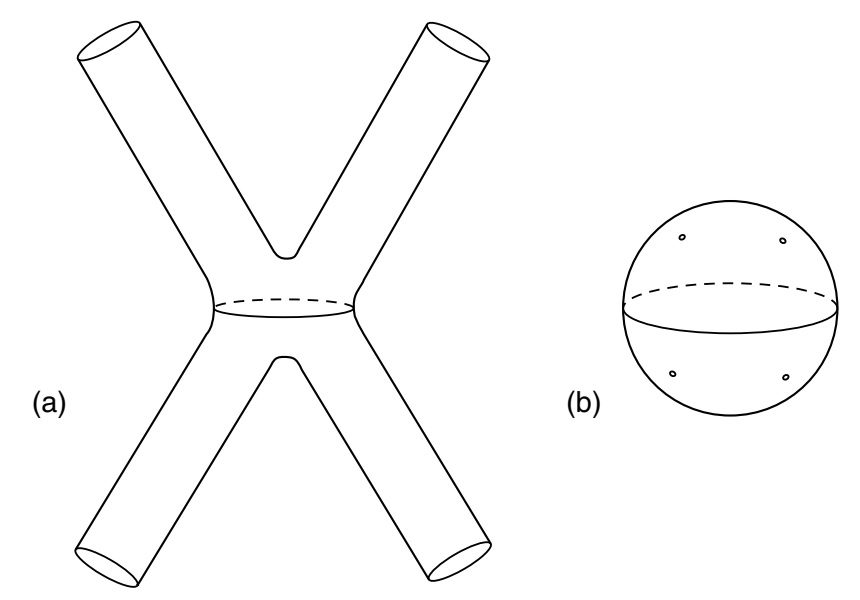
\includegraphics[width=0.8\textwidth]{figure/Fig3.8.jpg}\\
		\caption{(a) Scattering of closed strings, where the string sources tend toward $X^{0}=\pm \infty$. (b) Conformally equivalent image of 4-closed-string scattering: a sphere with very small holes.    }\label{Fig3.8}
	\end{center}
\end{figure}

So, we now examine the process shown in Figure \ref{Fig3.8}, where the sources are pulled to infinity. We will discuss how these sources should be represented in the path integral.    
Away from the scattering process, the strings propagate freely. Each outgoing and incoming string is a long cylinder, which can be described by a complex coordinate $w$,    
\begin{equation}
	-2 \pi t \leq \operatorname{Im} w \leq 0, \qquad w \cong w+2 \pi \:.
	\label{3.5.1} \end{equation}
The lower end of the cylinder, $\operatorname{Im} w=-2 \pi t$, is the end of the source, the upper end is inserted into the rest of the worldsheet, and the circumference is the periodic $\operatorname{Re} w$ direction. The limit corresponding to the scattering process is $t \rightarrow \infty$. It might seem that we are confusing long distances in spacetime with long cylinders in worldsheet coordinates, but this is quite correct: as we will see later, propagation over long spacetime distances originates precisely from such worldsheets where the cylinders become long in the above sense.    
We know from Chapter \ref{cha:2} that the cylinder has an equivalent description:    
\begin{equation}
	z=\exp (-\mi w), \quad \exp (-2 \pi t) \leq|z| \leq 1 \:. \label{3.5.2}
\end{equation}
In this picture, the long cylinder is mapped to a unit disc, where the external string state is the circle at the center.    
In the limit as $t \rightarrow \infty$, the small circle contracts to a point, and the worldsheet reduces to a sphere with a point inserted for each external state.    

\begin{figure}[!htbp]
	\begin{center}
		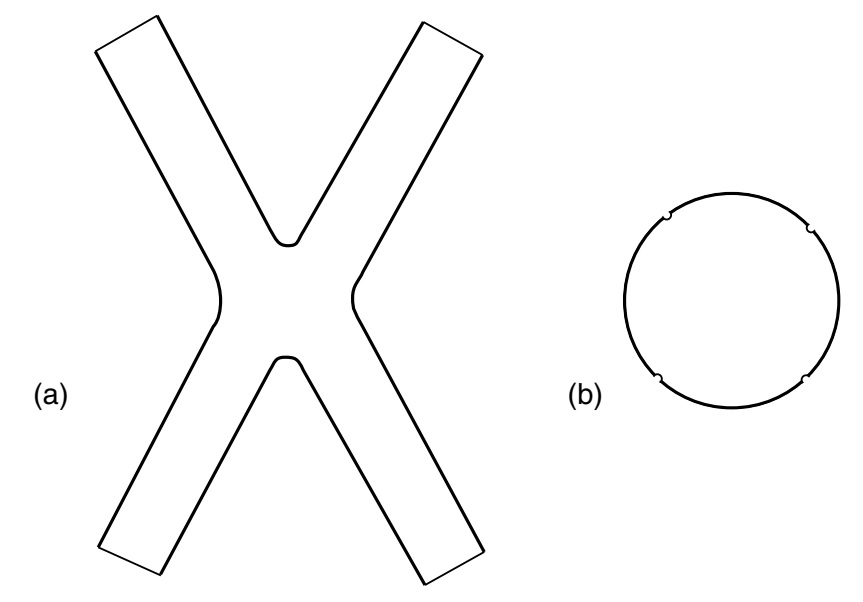
\includegraphics[width=0.8\textwidth]{figure/Fig3.9.jpg}\\
		\caption{(a) Scattering of four open strings, where the string sources tend toward $X^{0}=\pm \infty$. (b) Conformally equivalent image: a disc with indentations.    }\label{Fig3.9}
	\end{center}
\end{figure}

The same concept holds for external open string states.    
The long strip in Figure \ref{Fig3.9}a can be described as    
\begin{equation}
	-2 \pi t \leq \operatorname{Im} w \leq 0, \quad 0 \leq \operatorname{Re} w \leq \pi \:.
	\label{3.5.3} \end{equation}
where $\operatorname{Im} w=-2 \pi t$ is the source, and $\operatorname{Re} w=0, \pi$ are the endpoint boundaries. Under $z=-\exp (-\mi w)$, this maps to the intersection of the unit disc and the upper half-plane.    
A small semicircle is cut at the origin    
\begin{equation}
	\exp (-2 \pi t) \leq|z| \leq 1, \quad \operatorname{Im} z \geq 0 \:. \label{3.5.4}
\end{equation}
The scattering process now looks like Figure \ref{Fig3.9}b. In the limit $t \rightarrow \infty$, the source contracts to a point on the (endpoint) boundary.    

This is the state-operator correspondence we have already seen. Each source becomes a local perturbation on the worldsheet.    
For a given incoming or outgoing string, which has $D$-momentum $k^{\mu}$ and internal state $j$, there exists a corresponding local \emph{vertex operator} $\mathscr{V}_{j}(k)$ determined by the limiting process. Incoming and outgoing states are distinguished by the sign of $k^{0}$; for incoming states $k^{\mu}=(E, \mathbf{k})$ and outgoing states $k^{\mu}=-(E, \mathbf{k})$, Figures \ref{Fig3.8} and \ref{Fig3.9} only describe the lowest order amplitudes, but this construction is quite general: we can restrict our attention to compact worldsheets with no tubes tending to infinity, but with a point-like insertion in the interior for each external closed string.    
For each external open string, there is a point-like insertion on the boundary. Thus, a connected $n$-point $S$-matrix element is    
\begin{align}
	&S_{j_{1} \ldots j_{n}}(k_{1}, \ldots, k_{n})  \nonumber \\
	&\quad=\sum_{
		\text { compact } \atop \text { topologies}} \frac{[\dif X \, \dif g]}{V_{\text {diff } \times \text { Weyl }}} \exp (-S_{X}-\lambda \chi) 
	\prod_{i=1}^{n} \int \dif^{2} \sigma_{i} \: g(\sigma_{i})^{1 / 2} \mathscr{V}_{j_{i}}(k_{i}, \sigma_{i}) \:.
	\label{3.5.5} \end{align}
To make the vertex operator insertion diff-invariant, we integrate them over the worldsheet. In the rest of this volume, we will see that our guess is correct and defines a reasonable string $S$-matrix.    

Depending on which of the 4 theories we are examining, the sum over topologies may include unoriented worldsheets and/or worldsheets with boundaries. In general, the sum over topologies is not restricted to connected worldsheets; the overall process may include two or more independent particle scatterings. It is convenient to restrict the sum to connected worldsheets, focusing on the connected $S$-matrix.    

To obtain the connected $S$-matrix, we must sum over all compact, connected topologies of the worldsheet. In two dimensions, the classification of topologies is well-known. Any compact, connected, oriented surface without boundary is topologically equivalent to a sphere with $g$ handles, where $g$ is called the genus of the surface. In Figure \ref{Fig3.10}, we show the $g=0,1,2$ cases.    
\begin{figure}[!htbp]
	\begin{center}
		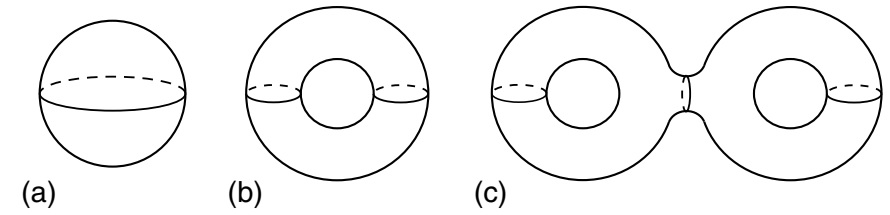
\includegraphics[width=0.8\textwidth]{figure/Fig3.10.jpg}\\
		\caption{Compact connected oriented closed surfaces with genus (a) 0, (b) 1, (c) 2 respectively.    }\label{Fig3.10}
	\end{center}
\end{figure}

Boundaries can be added by cutting holes in the closed surface. Any compact, connected, oriented two-dimensional surface is topologically equivalent to a sphere with $g$ handles and $b$ holes, for example $(g,b)=(0,1)$ is a disc, $(0,2)$ is an annulus, and $(0,3)$ is a pair of pants.    

To describe unoriented surfaces, it is useful to introduce cross-caps: cutting a hole in the surface and gluing opposite points together.    
In detail, taking complex coordinates, cut out a disc slightly smaller than unit radius, and glue together opposite points defined by $z^{\prime}=-1 / \bar{z}$. Since the gluing is anti-holomorphic, the resulting surface is unoriented. In addition, unlike the case of a boundary, a cross-cap does not introduce a boundary or other local features. Since the boundary produced by cutting is only the boundary of the coordinate patch, any compact connected closed surface, whether oriented or unoriented, can always be obtained by adding $g$ handles and $c$ cross-caps to a sphere; any compact connected surface can be obtained by adding $g$ handles, $b$ boundaries, and $c$ cross-caps.    
In fact, these descriptions are somewhat redundant: for both cases with and without boundaries, they can be obtained precisely by restricting the sum to only one of $g$ or $c$ being non-zero. For example, $(g, b, c) = (0, 0, 1)$ is a projective plane, $(g, b, c) = (0, 1, 1)$ is a Mobius strip, $(g, b, c) = (0, 0, 2)$ is a Klein bottle, and a torus with one cross-cap can be obtained via $(g, b, c) = (0, 0, 3)$ or $(g, b, c) = (1, 0, 1)$, with every two cross-caps being exchangeable for one handle.    
The Euler characteristic is    
\begin{equation}
	\chi=2-2 g-b-c \:. \label{3.5.6}
\end{equation}

The number of different topologies is much smaller than the number of different Feynman diagrams in a given order of field theory. For example, in closed oriented theory, in each order of perturbation theory, there exists exactly one topology. In field theory, the number of diagrams grows geometrically. A single string diagram includes all field theory diagrams. In different limits, handles are much longer than their circumference, we can approximate handles as lines, and string diagrams approximate corresponding Feynman diagrams in this limit.    

\section{\texorpdfstring{Vertex operators}{3.6 Vertex operators}} \label{sec:3.6}

Using the state-operator correspondence, the vertex operator for the closed string tachyon is    
\begin{align}
	V_{0} &=2 g_{\mathrm{c}} \int \dif^{2} \sigma \: g^{1 / 2} \,\me^{\mi k \cdot X}  \nonumber \\
	& \rightarrow g_{\mathrm{c}} \int \dif^{2} z\: : \mathrel{\me^{\mi k \cdot X}}: \:.
	\label{3.6.1} \end{align}
We introduced a factor $g_{\mathrm{c}}$ in the mapping. This is the closed string coupling constant, originating from adding an extra string to the process: we use the normalization of the vertex operator as the definition of the coupling. In the second line, we transition to a flat worldsheet. The vertex operator must be diff and Weyl invariant, so, in particular, it must be conformally invariant on a flat worldsheet. To cancel the transformation of $\dif^2 z$, the operator must be a tensor of weight $(1,1)$.\footnote{This will have important implications for \eqref{4.1.5}.}
Through a direct OPE calculation, $\me^{\mi k \cdot X}$ is a tensor of weight $h=\tilde{h}=\alpha^{\prime} k^{2} / 4$, so the condition is    
\begin{equation}
	m^{2}=-k^{2}=-\frac{4}{\alpha^{\prime}} \:, \label{3.6.2}
\end{equation}
which is exactly the mass discovered in light-cone quantization.    
Similarly, closed string tensor states at the first excited level have the flat-worldsheet vertex operator    
\begin{equation}
	\frac{2 g_{\mathrm{c}}}{\alpha^{\prime}} \int \dif^{2} z\: : \mathrel{\partial X^{\mu} \bar{\partial} X^{\nu} \me^{\mi k \cdot X}}: \:. \label{3.6.3}
\end{equation}
The normalization relative to the tachyon vertex operator originates from the state-operator correspondence, and as we will see in Chapter \ref{cha:6}, the same relative normalization is obtained from the normalization of the $S$-matrix.    
The weights are    
\begin{equation}
	h=\tilde{h}=1+\frac{\alpha^{\prime} k^{2}}{4} \:, \label{3.6.4}
\end{equation}
so they are massless, again consistent with light-cone quantization. For it to be a tensor, there are further conditions, which we will handle below.    
\subsubsection*{\Large Vertex operators in the Polyakov formalism}

Within the state-operator mapping, we have a systematic method to write down flat-worldsheet vertex operators for any state. Since the worldsheet can always be made flat, in principle, this is all we need. However, it is now useful to study vertex operators on curved worldsheets in the Polyakov framework. The method we use will be somewhat cumbersome and not as systematic as the state-operator mapping, but some results are useful.

Any operator included in the Polyakov path integral \eqref{3.5.5} must reflect the local diff $\times$ Weyl symmetry of the theory. We have not yet specified how the operator in the first line of (\ref{3.6.1}) is defined on the worldsheet. As in our previous discussion of the Weyl anomaly, it is convenient to use a method that automatically preserves diff invariance and then manually check the Weyl transformation. For most purposes, dimensional regularization is used in the literature. However, we do not have a great need for it here, so we will not introduce it; instead, we will generalize the normal ordering introduced earlier in \eqref{2.2.7}.

Define a renormalized operator:
\begin{equation}\label{3.6.5}
	[\mathscr{F}]_{\mathrm{r}}=\exp \left(\frac{1}{2} \int d^{2} \sigma d^{2} \sigma^{\prime} \Delta\left(\sigma, \sigma^{\prime}\right) \frac{\delta}{\delta X^{\mu}(\sigma)} \frac{\delta}{\delta X_{\mu}\left(\sigma^{\prime}\right)}\right) \mathscr{F}
\end{equation}
where
\begin{equation}
	\Delta\left(\sigma, \sigma^{\prime}\right)=\frac{\alpha^{\prime}}{2} \ln d^{2}\left(\sigma, \sigma^{\prime}\right)
\end{equation}
and $d\left(\sigma, \sigma^{\prime}\right)$ is the geodesic distance between $\sigma$ and $\sigma^{\prime}$.

Similar to normal ordering, (\ref{3.6.5}) tells us to sum over all ways of contracting pairs in $\mathscr{F}$ using $\Delta\left(\sigma, \sigma^{\prime}\right)$. On a flat worldsheet, $d^{2}\left(\sigma, \sigma^{\prime}\right)=\left|z-z^{\prime}\right|^{2}$ and this reduces to the conformal normal ordering we have studied carefully. On a curved worldsheet, it cancels the singular integrals from self-contractions of the fields in $\mathscr{F}$. Diff invariance is manifest, but the contractions depend on the metric. Introduce the Weyl variation:
\begin{equation}\label{3.6.7}
	\delta_{\mathrm{W}}[\mathscr{F}]_{\mathrm{r}}=\left[\delta_{\mathrm{W}} \mathscr{F}\right]_{\mathrm{r}}+\frac{1}{2} \int d^{2} \sigma d^{2} \sigma^{\prime} \delta_{\mathrm{W}} \Delta\left(\sigma, \sigma^{\prime}\right) \frac{\delta}{\delta X^{\mu}(\sigma)} \frac{\delta}{\delta X_{\mu}\left(\sigma^{\prime}\right)}[\mathscr{F}]_{\mathrm{r}}
\end{equation}
The first term represents the explicit Weyl variation in the operator. For the vertex operator of a state with momentum $k_\mu$, under translation, it must transform in the same way as the state, and thus takes the form of $e^{ik\cdot X}$ multiplied by derivatives of $X^\mu$. Operators with different numbers of derivatives do not mix under Weyl transformations.
\begin{tcolorbox}[breakable]
	\begin{proof}
		\begin{align}
			\delta_{\mathrm{W}}[\mathcal{F}]_{\mathrm{r}} & =\delta_{\mathrm{W}} e^{\frac{1}{2} \int d^2 \sigma d^2 \sigma^{\prime} \Delta\left(\sigma, \sigma^{\prime}\right) \frac{\delta}{\delta X^\mu(\sigma)} \frac{\delta}{\delta X_\mu\left(\sigma^{\prime}\right)}} \mathcal{F} \nonumber\\
			& =\delta_{\mathrm{W}}\left[\frac{1}{2} \int d^2 \sigma d^2 \sigma^{\prime} \Delta\left(\sigma, \sigma^{\prime}\right) \frac{\delta}{\delta X^\mu(\sigma)} \frac{\delta}{\delta X_\mu\left(\sigma^{\prime}\right)}\right] e^{\frac{1}{2} \int d^2 \sigma d^2 \sigma^{\prime} \Delta\left(\sigma, \sigma^{\prime}\right) \frac{\delta}{\delta X^\mu(\sigma)} \frac{\delta}{\delta X_\mu\left(\sigma^{\prime}\right)}} \mathcal{F} \nonumber\\
			& \quad + e^{\frac{1}{2} \int d^2 \sigma d^2 \sigma^{\prime} \Delta\left(\sigma, \sigma^{\prime}\right) \frac{\delta}{\delta X^\mu(\sigma)} \frac{\delta}{\delta X_\mu\left(\sigma^{\prime}\right)}} \delta_{\mathrm{W}} \mathcal{F} \nonumber\\
			& =\frac{1}{2} \int d^2 \sigma d^2 \sigma^{\prime}\left(\delta_{\mathrm{W}} \Delta\left(\sigma, \sigma^{\prime}\right)\right) \frac{\delta}{\delta X^\mu(\sigma)} \frac{\delta}{\delta X_\mu\left(\sigma^{\prime}\right)}[\mathcal{F}]_{\mathrm{r}}+\left[\delta_{\mathrm{W}} \mathcal{F}\right]_{\mathrm{r}}
		\end{align}
	\end{proof}
\end{tcolorbox}
We begin by examining the zero-derivative case, operator (\ref{3.6.1}). The Weyl variation originates from the explicit $g^{1/2}$ factor and the renormalization given in (\ref{3.6.7}):
\begin{equation}\label{3.6.8}
	\delta_{\mathrm{W}} V_{0}=2 g_{\mathrm{c}} \int d^{2} \sigma g^{1 / 2}\left(2 \delta \omega(\sigma)-\frac{k^{2}}{2} \delta_{\mathrm{W}} \Delta(\sigma, \sigma)\right)\left[e^{i k \cdot X(\sigma)}\right]_{\mathrm{r}}
\end{equation}

\begin{tcolorbox}[breakable]
	\begin{proof}
		with \(\delta_W g_{ab} = 2\delta \omega g_{ab}\) we find, using \eqref{3.6.7}
			\begin{align}
				\delta_W V_0 &= 2g_c \int d^2 \sigma \delta_W \sqrt{g} \left[ e^{ik \cdot X(\sigma)} \right]_r\nonumber \\
				&= 2g_c \int d^2 \sigma \left\{ \frac{1}{2} g^{-1/2} g^{ab} 2\delta \omega g_{ab} \left[ e^{ik \cdot X(\sigma)} \right]_r + \sqrt{g} \left[ \delta_W e^{ik \cdot X(\sigma)} \right]_r \right. \nonumber\\
				&\qquad \left. + \frac{1}{2} \sqrt{g} \int d^2 \sigma' d^2 \sigma'' \delta_W \Delta(\sigma', \sigma'') \frac{\delta}{\delta X^\mu(\sigma')} \frac{\delta}{\delta X_\mu(\sigma'')} \left[ e^{ik \cdot X(\sigma)} \right]_r \right\} \nonumber\\
				&= 2g_c \int d^2 \sigma \left\{ \sqrt{g} 2\delta \omega \left[ e^{ik \cdot X(\sigma)} \right]_r \right. \nonumber\\
				&\qquad \left. + \frac{1}{2} \sqrt{g} \int d^2 \sigma' d^2 \sigma'' \delta_W \Delta(\sigma', \sigma'') (-k^2) \delta^2 (\sigma - \sigma') \delta^2 (\sigma - \sigma'') \left[ e^{ik \cdot X(\sigma)} \right]_r \right\} \nonumber\\
				&= 2g_c \int d^2 \sigma \left\{ \sqrt{g} 2\delta \omega \left[ e^{ik \cdot X(\sigma)} \right]_r - \frac{k^2}{2} \sqrt{g} \delta_W \Delta(\sigma, \sigma) \left[ e^{ik \cdot X(\sigma)} \right]_r \right\} \nonumber\\
				&= 2g_c \int d^2 \sigma \sqrt{g} \left( 2\delta \omega - \frac{k^2}{2} \delta_W \Delta(\sigma, \sigma) \right) \left[ e^{ik \cdot X(\sigma)} \right]_r
			\end{align}
	\end{proof}
\end{tcolorbox}
At short distances,
\begin{equation}
	d^{2}\left(\sigma, \sigma^{\prime}\right) \approx\left(\sigma-\sigma^{\prime}\right)^{2} \exp (2 \omega(\sigma))
\end{equation}
consequently,
\begin{equation}
	\Delta\left(\sigma, \sigma^{\prime}\right) \approx \alpha^{\prime} \omega(\sigma)+\frac{\alpha^{\prime}}{2} \ln \left(\sigma-\sigma^{\prime}\right)^{2}
\end{equation}
In the limit $\sigma^{\prime} \rightarrow \sigma$, the Weyl variation is non-singular:
\begin{equation}\label{3.6.11}
	\delta_{\mathrm{W}} \Delta(\sigma, \sigma)=\alpha^{\prime} \delta \omega(\sigma)
\end{equation}
The condition for the Weyl variation (\ref{3.6.8}) to be zero is $k^{2}=4 / \alpha^{\prime}$, exactly the result derived previously.
\begin{tcolorbox}[breakable]
	\begin{proof}
		Assuming the geodesic distance $d$ can be given as line integral over the geodesic $\gamma$ as:
		\begin{equation}
			d(\sigma, \sigma') = \int_{\gamma} d\lambda\sqrt{e^{2w(\lambda)}\delta_{ab}\dv{x^a}{\lambda}\dv{x^b}{\lambda}}= \int_{\lambda(\sigma)}^{\lambda(\sigma')} d\lambda e^{w(\lambda)}\abs{\dv{z}{\lambda}}=\int_\sigma^{\sigma'} dz\,e^{w(z)}
		\end{equation}
		Upon taylor series expanding $w(z)$ upto second order:
		\begin{align}
			d(\sigma, \sigma') &= e^{w(\sigma)} \int_\sigma^{\sigma'} dz ~ e^{(z-\sigma).\partial w(\sigma) + \frac{1}{2}(z-\sigma)^a(z-\sigma)^b [\partial_a \partial_b w(\sigma)+(\partial_a w)(\partial_b w)]+\ldots}\notag\\
			& = e^{w(\sigma)} \int_\sigma^{\sigma'} dz ~ ( 1 + (z-\sigma).\partial w(\sigma) + \frac{1}{2}(z-\sigma)^a(z-\sigma)^b[\partial_a \partial_b w(\sigma)%+(\partial_a w)(\partial_b w)]
			+\ldots) \notag\\
			&=e^{w(\sigma)} |\sigma' - \sigma|\left(1 + \frac{1}{2}(\sigma'-\sigma).\partial w(\sigma) +  \frac{1}{6}(\sigma'-\sigma)^a(\sigma'-\sigma)^b[\partial_a \partial_b w(\sigma)%+(\partial_a w)(\partial_b w)]
			+\ldots\right)\notag\\
			&= e^{w(\sigma)} |\sigma' - \sigma| e^{\frac{1}{2}(\sigma'-\sigma).\partial w(\sigma) +  \frac{1}{6}(\sigma'-\sigma)^a(\sigma'-\sigma)^b[\partial_a \partial_b w(\sigma)+(\partial_a w)(\partial_b w)]+\ldots} 
		\end{align}		
		So, now, we get, with $\Delta (\sigma, \sigma') = \frac{\alpha'}{2} \ln d^2(\sigma, \sigma')$:
		
		$$\Delta (\sigma, \sigma') =\alpha'(w(\sigma) + \frac{1}{2}(\sigma'-\sigma).\partial w(\sigma) +  \frac{1}{6}(\sigma'-\sigma)^a(\sigma'-\sigma)^b[\partial_a \partial_b w(\sigma)+(\partial_a w)(\partial_b w)]+\ldots$$
		Notice that $\Delta (\sigma, \sigma')$ is not symmetric in $\sigma, \sigma'$, so we need to symmetrise it. Thus we can write $\Delta$ as :
		\begin{multline}
			\Delta (\sigma, \sigma') =\alpha'\bigg( \frac{1}{2} [w(\sigma) + w(\sigma') ] + \frac{1}{4}(\sigma'-\sigma).[\partial w(\sigma) - \partial^{'} w(\sigma')] \\+  \frac{1}{12}(\sigma'-\sigma)^a(\sigma'-\sigma)^b[\partial_a \partial_bw(\sigma)+\partial^{'}_a \partial_b^{'}w(\sigma')]\bigg)
		\end{multline}
		Hence we find in the limit $\sigma'\to\sigma$:
		\begin{equation}
		\delta_{\mathrm{W}} \Delta(\sigma, \sigma)\approx\alpha^{\prime} \delta \omega(\sigma)
		\end{equation}
	\end{proof}
\end{tcolorbox}
\subsubsection*{\Large Off-shell amplitudes}

Consider a naive attempt to define off-shell amplitudes by taking $k^\mu$ not on the mass shell. This is inconsistent with local worldsheet symmetry. In position space, this corresponds to a local probe of the string worldsheet, given by an insertion:
\begin{equation}\label{3.6.12}
	\delta^{D}\left(X(\sigma)-x_{0}\right)=\int \frac{d^{D} k}{(2 \pi)^{D}} \exp \left[i k \cdot\left(X(\sigma)-x_{0}\right)\right]
\end{equation}
Since this contains all momenta, it is inconsistent. From several perspectives, this is not surprising. First, the previous discussion—that our point sources (vertex operators) for string states require a limiting process—remarkably restricts us to on-shell problems. Second, string theory contains gravity, and simple off-shell amplitudes do not exist in general relativity because we cannot specify the position of the probe without non-physical coordinates; coordinate-invariant off-shell quantities are much more complex. Third, in string theory, we have not introduced additional fields to measure local observables (similar to the electroweak processes used to probe strong interactions): we must use the string itself or other objects inherent in the theory (D-branes and solitons).

At least in perturbation theory, off-shell amplitudes can be defined. If we fix the gauge (for which light-cone gauge is simplest) and use string sources, then the S-matrix can be derived using a reduction formula \eqref{3.5.5} similar to quantum field theory. Finite-time transition amplitudes can be defined before taking the infinite-time limit. Incidentally, readers attempting to link the current discussion to field theory should note that the path integral expression \eqref{3.5.5} is not like a Green's function but rather has S-matrix element properties. The analogous object in field theory is a Green's function where external propagators are truncated and external momenta are restricted to the mass shell.

The discussion of local probes (\ref{3.6.12}) also points to the problem of contact interactions between strings. The simplest form of such an interaction would be:
\begin{equation}
	\int_{M} d^{2} \sigma g(\sigma)^{1 / 2} \int_{M} d^{2} \sigma^{\prime} g\left(\sigma^{\prime}\right)^{1 / 2} \delta^{D}\left(X(\sigma)-X\left(\sigma^{\prime}\right)\right)
\end{equation}
This is non-zero as long as the worldsheet intersects itself. However, the $\delta$-function contains all momenta, as in (\ref{3.6.12}). Thus, it is not Weyl invariant. The structure of string theory is quite fixed: strings can only couple to other strings in the manner described at the beginning of this chapter.

\subsubsection*{\Large Massless closed string vertex operators}

While somewhat messy, it is interesting to further pursue the Polyakov treatment of vertex operators. There is no way to construct a worldsheet scalar with exactly one derivative. Therefore, the next case is two derivatives; the possible diff-invariant cases are:
\begin{equation}\label{3.6.14}
\begin{aligned}
		V_{1}=\frac{g_{\mathrm{c}}}{\alpha^{\prime}} \int d^{2} \sigma g^{1 / 2}\Big\{\left(g^{a b} s_{\mu \nu}+i \epsilon^{a b} a_{\mu \nu}\right)&\left[\partial_{a} X^{\mu} \partial_{b} X^{v} e^{i k \cdot X}\right]_{\mathrm{r}}+\alpha^{\prime} \phi R\left[e^{i k \cdot X}\right]_{\mathrm{r}}\Big\}
\end{aligned}
\end{equation}
where $s_{\mu \nu}, a_{\mu \nu}$, and $\phi$ are a symmetric matrix, an antisymmetric matrix, and a constant, respectively.

The antisymmetric tensor $\epsilon^{ab}$ is normalized such that $g^{1/2}\epsilon^{12}=1$, or $g^{1/2}\epsilon^{z\bar{z}}=-i$. The $i$ accompanying the antisymmetric tensor in the vertex operator can be understood as arising from Euclidean continuation, because this term must have an odd number (one) of time derivatives. This result is widely applied in Euclidean actions and vertex operators. To extend the Weyl invariance analysis, we need to solve the higher-order geodesic distance Weyl correlation (\ref{3.6.11}).

\begin{subequations}\label{3.6.15}
	\begin{equation}
		\left.\partial_{a} \delta_{\mathrm{W}} \Delta\left(\sigma, \sigma^{\prime}\right)\right|_{\sigma^{\prime}=\sigma}=\frac{1}{2} \alpha^{\prime} \partial_{a} \delta \omega(\sigma)
	\end{equation}
	\begin{equation}
		\left.\partial_{a} \partial_{b}^{\prime} \delta_{\mathrm{W}} \Delta\left(\sigma, \sigma^{\prime}\right)\right|_{\sigma^{\prime}=\sigma}=\frac{1+\gamma}{2} \alpha^{\prime} \nabla_{a} \partial_{b} \delta \omega(\sigma)
	\end{equation}
	\begin{equation}
		\left.\nabla_{a} \partial_{b} \delta_{\mathrm{W}} \Delta\left(\sigma, \sigma^{\prime}\right)\right|_{\sigma^{\prime}=\sigma}=-\frac{\gamma}{2} \alpha^{\prime} \nabla_{a} \partial_{b} \delta \omega(\sigma)
	\end{equation}
\end{subequations}
where $\gamma = -2/3$. We leave it as a parameter for later reference; the third equation can be obtained from the gradient of the second or first. For the variation of curvature, we use \eqref{3.3.5}. 
\begin{tcolorbox}[breakable]
	\begin{proof}
		We found $\Delta(\sigma,\sigma')$ earlier as:
		\begin{multline}
			\Delta (\sigma, \sigma') =\alpha'\bigg( \frac{1}{2} [w(\sigma) + w(\sigma') ] + \frac{1}{4}(\sigma'-\sigma).[\partial w(\sigma) - \partial^{'} w(\sigma')] \\+  \frac{1}{12}(\sigma'-\sigma)^a(\sigma'-\sigma)^b[\partial_a \partial_bw(\sigma)+\partial^{'}_a \partial_b^{'}w(\sigma')]\bigg)
		\end{multline}
		Taking the derivative of $\delta_W\Delta$ wrt $\sigma'_b$:
		\begin{multline}
			\partial^{'}_b \delta_W \Delta (\sigma, \sigma') =\alpha'\bigg( \frac{1}{2}\partial^{'}_b \delta w(\sigma') +  \frac{1}{4}[\partial_b w(\sigma) - \partial^{'}_b w(\sigma')]  - \frac{1}{4}(\sigma' - \sigma)^a \partial'_a \partial_b'w(\sigma')\\
			+ \frac{1}{6}(\sigma' - \sigma)^a[\partial_a \partial_bw(\sigma)+\partial^{'}_a \partial_b^{'}w(\sigma')]\bigg) + \mathcal{O}(\sigma - \sigma')^2
		\end{multline}
		The derivative wrt $\partial_b$ is same as above, therefore dropping the prime and taking $\sigma' \rightarrow \sigma$:
		\begin{equation}
				\left.\partial_{a} \delta_{\mathrm{W}} \Delta\left(\sigma, \sigma^{\prime}\right)\right|_{\sigma^{\prime}=\sigma}=\frac{1}{2} \alpha^{\prime} \partial_{a} \delta \omega(\sigma)
		\end{equation}
		Similarly, taking derivative with respect to $\sigma_a$:
		
		\begin{multline}
			\partial_a \partial^{'}_b \delta_W \Delta (\sigma, \sigma') =\alpha'\bigg( \frac{1}{4}[\partial_a \partial_b \delta w(\sigma)+ \partial^{'}_a \partial^{'}_b \delta w(\sigma')] -  \frac{1}{6}[\partial_a \partial_b \delta w(\sigma)+ \partial^{'}_a \partial^{'}_b \delta w(\sigma')]\bigg)\\
			+ \order{\sigma - \sigma'}
		\end{multline}
		Thus, finally, when $\sigma' \rightarrow \sigma$, we have: 
		
		\begin{align}
			\partial_a \partial^{'}_b \delta_W \Delta (\sigma, \sigma')=  \frac{\alpha'}{6}\partial_a \partial_b\delta w(\sigma)
		\end{align}
		For the last expression,
		\begin{align}
			\partial_b \partial_a \delta_w \Delta(\sigma,\sigma') 
			&= \alpha' \partial_b \Bigg[
			\frac{1}{2} \partial_a \delta w(\sigma)
			- \frac{1}{4} \big( \partial_a \delta w(\sigma) - \partial'_a \delta w(\sigma') \big)
			+ \frac{1}{4} (\sigma' - \sigma)^c \partial_a \partial_c \delta w(\sigma) \nonumber \\
			&\qquad\quad
			- \frac{1}{6} (\sigma' - \sigma)^c \big( \partial_a \partial_c \delta w(\sigma)
			+ \partial'_a \partial'_c \delta w(\sigma') \big)
			+ \mathcal{O}\big((\sigma' - \sigma)^2\big)
			\Bigg] \nonumber \\
			&= \alpha' \Bigg[
			\frac{1}{2} \partial_a \partial_b \delta w(\sigma)
			- \frac{1}{4} \partial_a \partial_b \delta w(\sigma)
			- \frac{1}{4} \partial_a \partial_b \delta w(\sigma) \nonumber \\
			&\qquad\quad
			+ \frac{1}{6} \big( \partial_a \partial_b \delta w(\sigma)
			+ \partial'_a \partial'_b \delta w(\sigma') \big)
			+ \mathcal{O}(\sigma' - \sigma)
			\Bigg] \nonumber \\
			&= \frac{1}{3} \alpha' \partial_a \partial_b \delta w(\sigma)
			+ \mathcal{O}(\sigma' - \sigma)
		\end{align}
		Taking $\sigma' \to \sigma$, we find
		\begin{align}
			\partial_a \partial_b \delta_w \Delta(\sigma,\sigma')\Big|_{\sigma' \to \sigma}
			= \frac{1}{3} \alpha' \nabla_a \partial_b \delta w(\sigma)
			\tag{3.165}
		\end{align}
	\end{proof}
\end{tcolorbox}


For renormalization variation, we use (\ref{3.6.7}) and (\ref{3.6.15}).

\begin{equation}\label{3.6.16}
	\begin{array}{c}
		\delta_{\mathrm{W}} V_{1}=\frac{g_{\mathrm{c}}}{2} \int d^{2} \sigma g^{1 / 2} \delta \omega\Big\{\left(g^{a b} S_{\mu v}+i \epsilon^{a b} A_{\mu v}\right)\left[\partial_{a} X^{\mu} \partial_{b} X^{v} e^{i k \cdot X}\right]_{\mathrm{r}}+\alpha^{\prime} F R\left[e^{i k \cdot X}\right]_{\mathrm{r}}\Big\}
	\end{array}
\end{equation}
where
\begin{subequations}
	\begin{equation}
		S_{\mu v}=-k^{2} s_{\mu v}+k_{v} k^{\omega} S_{\mu \omega}+k_{\mu} k^{\omega} s_{v \omega}-(1+\gamma) k_{\mu} k_{v} s_{\omega}^{\omega}+4 k_{\mu} k_{v} \phi
	\end{equation}
	\begin{equation}
		A_{\mu v}=-k^{2} a_{\mu \nu}+k_{v} k^{\omega} a_{\mu \omega}-k_{\mu} k^{\omega} a_{v \omega}
	\end{equation}
	\begin{equation}
		F=(\gamma-1) k^{2} \phi+\frac{1}{2} \gamma k^{\mu} k^{v} s_{\mu v}-\frac{1}{4} \gamma(1+\gamma) k^{2} s_{v}^{v}
	\end{equation}\label{3.6.17}
\end{subequations}
\begin{tcolorbox}[breakable]
		Some preliminaries first. Under an infinitesimal Weyl transformation
		\begin{align}
			\delta_{\mathrm{W}} g_{a b} &= 2 \delta \omega g_{a b} \\
			\delta_{\mathrm{W}} g^{a b} &= -2 \delta \omega g^{a b}
		\end{align}
		we also have
		\begin{align}
			\delta_{\mathrm{W}} \sqrt{g} &= \frac{1}{2} g^{-1/2} \delta_{\mathrm{W}} g = \frac{1}{2} g^{-1/2} g g^{a b} \delta_{\mathrm{W}} g_{a b} = \frac{1}{2} g^{-1/2} g g^{a b} 2 \delta \omega g_{a b} = \sqrt{g} 2 \delta \omega
		\end{align}
		and
		\begin{align}
			\delta_{\mathrm{W}}\left(\sqrt{g} g^{a b}\right) &= \delta_{\mathrm{W}}(\sqrt{g}) g^{a b} + \sqrt{g} \delta_{\mathrm{W}} g^{a b} = \sqrt{g} 2 \delta \omega g^{a b} - 2 \sqrt{g} \delta \omega g^{a b} = 0
		\end{align}
		This implies that the antisymmetric tensor $\epsilon^{a b}$ also transforms non-trivially under a Weyl transformation. Indeed, from $\sqrt{g} \epsilon^{12}=1$ we have
		\begin{align}
			\left(\delta_{\mathrm{W}} \sqrt{g}\right) \epsilon^{12} + \sqrt{g}\left(\delta_{\mathrm{W}} \epsilon^{12}\right) = 0 \Rightarrow \delta_{\mathrm{W}} \epsilon^{12} = -2 \delta \omega \epsilon^{12}
		\end{align}
		and thus more generally
		\begin{align}
			\delta_{\mathrm{W}} \epsilon^{a b} = -2 \delta \omega \epsilon^{a b}
		\end{align}
		But we will only need the relation
		\begin{align}
			\delta_{\mathrm{W}}\left(\sqrt{g} \epsilon^{a b}\right) = 0
		\end{align}
		From (1.2.32) we also know that $\sqrt{g'} R' = \sqrt{g}(R - 2 \nabla^2 \delta \omega)$ so that
		\begin{align}
			\delta_{\mathrm{W}}(\sqrt{g} R) = -2 \sqrt{g} \nabla^2 \delta \omega
		\end{align}
		
		After all these preliminaries, let us now work out Weyl transformation of \eqref{3.6.14}, using the above and also \eqref{3.6.7}
		
		\begin{align}
			\delta_{\mathrm{W}} V_1 &= \frac{g_c}{\alpha'} \int d^2 \sigma\left\{\left(\delta_{\mathrm{W}}\left(\sqrt{g} g^{a b}\right) s_{\mu \nu}+i \delta_{\mathrm{W}}\left(\sqrt{g} \epsilon^{a b}\right) a_{\mu \nu}\right)\left[\partial_a X^\mu \partial_b X^\nu e^{i k \cdot X(\sigma)}\right]_{\mathrm{r}}\right. \nonumber \\
			&\quad + \alpha' \phi \delta_{\mathrm{W}}(\sqrt{g} R)\left[e^{i k \cdot X(\sigma)}\right]_{\mathrm{r}}  + \sqrt{g}\left(g^{a b} s_{\mu \nu}+i \epsilon^{a b} a_{\mu \nu}\right) \frac{1}{2} \int d^2 \sigma^{\prime} d^2 \sigma^{\prime \prime} \delta_{\mathrm{W}} \Delta\left(\sigma^{\prime}, \sigma^{\prime \prime}\right) \nonumber\\
			&\qquad\times \frac{\delta}{\delta X^\lambda\left(\sigma^{\prime}\right)}\frac{\delta}{\delta X_\lambda\left(\sigma^{\prime \prime}\right)}\left[\partial_a X^\mu \partial_b X^\nu e^{i k \cdot X(\sigma)}\right]_{\mathrm{r}} \nonumber \\
			&\left.\quad + \sqrt{g} \alpha' \phi R \frac{1}{2} \int d^2 \sigma^{\prime} d^2 \sigma^{\prime \prime} \delta_{\mathrm{W}} \Delta\left(\sigma^{\prime}, \sigma^{\prime \prime}\right) \frac{\delta}{\delta X^\lambda\left(\sigma^{\prime}\right)} \frac{\delta}{\delta X_\lambda\left(\sigma^{\prime \prime}\right)}\left[e^{i k \cdot X(\sigma)}\right]_{\mathrm{r}}\right\}
		\end{align}
		Recall that $\delta_{\mathrm{W}} e^{i k \cdot X(\sigma)} = \delta_{\mathrm{W}} \partial_a X^\mu \partial_b X^\nu e^{i k \cdot X(\sigma)} = 0$, as there is no metric dependence in these operators. We have just seen that the first line vanishes and so can write
		
		\begin{align}
			\delta_{\mathrm{W}} V_1 &= \frac{g_c}{\alpha'} \int d^2 \sigma\left\{-2 \alpha' \phi \sqrt{g}\left(\nabla^2 \delta \omega\right)\left[e^{i k \cdot X(\sigma)}\right]_{\mathrm{r}}\right. + \frac{1}{2} \sqrt{g}\left(g^{a b} s_{\mu \nu}+i \epsilon^{a b} a_{\mu \nu}\right)\nonumber \\
			&\quad \times  \int d^2 \sigma^{\prime} d^2 \sigma^{\prime \prime} \delta_{\mathrm{W}} \Delta\left(\sigma^{\prime}, \sigma^{\prime \prime}\right)\frac{\delta}{\delta X^\lambda\left(\sigma^{\prime}\right)} \frac{\delta}{\delta X_\lambda\left(\sigma^{\prime \prime}\right)}\left[\partial_a X^\mu \partial_b X^\nu e^{i k \cdot X(\sigma)}\right]_{\mathrm{r}} \nonumber \\
			&\left.\quad + \frac{1}{2} \sqrt{g} \alpha' \phi R \int d^2 \sigma^{\prime} d^2 \sigma^{\prime \prime} \delta_{\mathrm{W}} \Delta\left(\sigma^{\prime}, \sigma^{\prime \prime}\right) \frac{\delta}{\delta X^\lambda\left(\sigma^{\prime}\right)} \frac{\delta}{\delta X_\lambda\left(\sigma^{\prime \prime}\right)}\left[e^{i k \cdot X(\sigma)}\right]_{\mathrm{r}}\right\}\label{3.175}
		\end{align}
		Let us for convenience work out the different lines separately. We start with the first line
		\begin{align}
			\mathcal{J}_1 &= -2 g_c \phi \int d^2 \sigma \sqrt{g}\left(\nabla^2 \delta \omega\right)\left[e^{i k \cdot X(\sigma)}\right]_{\mathrm{r}} = -2 g_c \phi \int d^2 \sigma \sqrt{g}\left(\nabla_a \partial^a \delta \omega\right)\left[e^{i k \cdot X(\sigma)}\right]_{\mathrm{r}} \nonumber \\
			&= -2 g_c \phi \int d^2 \sigma \sqrt{g}\left\{\nabla_a\left(\partial^a \delta \omega\left[e^{i k \cdot X(\sigma)}\right]_{\mathrm{r}}\right) - \partial^a \delta \omega \nabla_a\left[e^{i k \cdot X(\sigma)}\right]_{\mathrm{r}}\right\} \nonumber \\
			&= -2 g_c \phi \int d^2 \sigma \partial_a\left(\sqrt{g} \partial^a \delta \omega\left[e^{i k \cdot X(\sigma)}\right]_{\mathrm{r}}\right) + 2 g_c \phi \int d^2 \sigma \sqrt{g} \partial^a \delta \omega \nabla_a\left[e^{i k \cdot X(\sigma)}\right]_{\mathrm{r}} \nonumber \\
			&= + 2 g_c \phi \int d^2 \sigma \sqrt{g} \partial^a \delta \omega \nabla_a\left[e^{i k \cdot X(\sigma)}\right]_{\mathrm{r}}
		\end{align}
		where we have used $\partial_a(\sqrt{g} v^a) = \sqrt{g} \nabla_a v^a$ and $\nabla_a \sqrt{g} = 0$. We can now replace the covariant derivative by a partial derivative as it acts on a scalar and partial integrate the other derivative
		\begin{align}
			\mathcal{J}_1 &= -2 g_c \phi \int d^2 \sigma \delta \omega \partial^a\left(\sqrt{g} \partial_a\left[e^{i k \cdot X(\sigma)}\right]_{\mathrm{r}}\right) \nonumber \\
			&= -2 g_c \phi \int d^2 \sigma \delta \omega \sqrt{g} \nabla^a \partial_a\left[e^{i k \cdot X(\sigma)}\right]_{\mathrm{r}}
		\end{align}
		We now have
		\begin{align}
			\nabla^a \partial_a e^{i k \cdot X} &= \nabla^a\left(i k^\mu \partial_a X_\mu\right) e^{i k \cdot X} \nonumber \\
			&= i k^\mu\left(\nabla^a \partial_a X_\mu\right) e^{i k \cdot X} + \left(i k^\mu \partial_a X_\mu\right)\left(i k^\nu \nabla^a X_\nu\right) e^{i k \cdot X} \nonumber \\
			&= i k^\mu \nabla^2 X_\mu e^{i k \cdot X} - k^\mu k^\nu \partial_a X_\mu \partial^a X_\nu e^{i k \cdot X}
		\end{align}
		We have freely replaced $\partial_a$ by $\nabla_a$ and vice-versa when they are acting on worldsheet scalars. Therefore, using \eqref{3.6.18},
		\begin{align}
			\left[\nabla^a \partial_a e^{i k \cdot X}\right]_{\mathrm{r}} &= i k^\mu\left[\nabla^2 X_\mu e^{i k \cdot X}\right]_{\mathrm{r}} - k^\mu k^\nu\left[\partial_a X_\mu \partial^a X_\nu e^{i k \cdot X}\right]_{\mathrm{r}} \nonumber \\
			&= i k^\mu \times\left(-i \frac{\alpha'}{6} k_\mu R\left[e^{i k \cdot X(\sigma)}\right]_{\mathrm{r}}\right) - k^\mu k^\nu\left[\partial_a X_\mu \partial^a X_\nu e^{i k \cdot X}\right]_{\mathrm{r}} \nonumber \\
			&= \frac{\alpha'}{6} k^2 R\left[e^{i k \cdot X(\sigma)}\right]_{\mathrm{r}} - k^\mu k^\nu g^{a b}\left[\partial_a X_\mu \partial_b X_\nu e^{i k \cdot X}\right]_{\mathrm{r}}
		\end{align}
		and thus
		\begin{align}
			\mathcal{J}_1 &= -\frac{g_c \alpha'}{3} k^2 \phi \int d^2 \sigma \sqrt{g} \delta \omega R\left[e^{i k \cdot X(\sigma)}\right]_{\mathrm{r}} + 2 g_c k^\mu k^\nu \phi \int d^2 \sigma \sqrt{g} \delta \omega g^{a b}\left[\partial_a X_\mu \partial_b X_\nu e^{i k \cdot X}\right]_{\mathrm{r}} \nonumber \\
			&= \frac{g_c}{2} \int d^2 \sigma \sqrt{g} \delta \omega\left\{-\frac{2 \alpha'}{3} k^2 \phi R\left[e^{i k \cdot X(\sigma)}\right]_{\mathrm{r}} + g^{a b}\left(4 k^\mu k^\nu \phi\right)\left[\partial_a X_\mu \partial_b X_\nu e^{i k \cdot X}\right]_{\mathrm{r}}\right\}\label{3.179}
		\end{align}
		Before we tackle the second, more difficult, line of \eqref{3.175}, let us do the easier third line
		\begin{align}
			\mathcal{J}_3 &= \frac{g_c}{2} \phi \int d^2 \sigma d^2 \sigma^{\prime} d^2 \sigma^{\prime \prime} \sqrt{g} R \delta_{\mathrm{W}} \Delta\left(\sigma^{\prime}, \sigma^{\prime \prime}\right) \frac{\delta}{\delta X^\lambda\left(\sigma^{\prime}\right)} \frac{\delta}{\delta X_\lambda\left(\sigma^{\prime \prime}\right)}\left[e^{i k \cdot X(\sigma)}\right]_{\mathrm{r}} \nonumber \\
			&= \frac{g_c}{2} \phi \int d^2 \sigma d^2 \sigma^{\prime} d^2 \sigma^{\prime \prime} \sqrt{g} R \delta_{\mathrm{W}} \Delta\left(\sigma^{\prime}, \sigma^{\prime \prime}\right)\left(-k^2\right) \delta^2\left(\sigma-\sigma^{\prime}\right) \delta^2\left(\sigma-\sigma^{\prime \prime}\right)\left[e^{i k \cdot X(\sigma)}\right]_{\mathrm{r}} \nonumber \\
			&= -\frac{g_c}{2} \phi k^2 \int d^2 \sigma \sqrt{g} R \delta_{\mathrm{W}} \Delta(\sigma, \sigma)\left[e^{i k \cdot X(\sigma)}\right]_{\mathrm{r}} = -\frac{g_c}{2} \phi k^2 \int d^2 \sigma \sqrt{g} R \alpha^{\prime} \delta \omega\left[e^{i k \cdot X(\sigma)}\right]_{\mathrm{r}} \nonumber \\
			&= \frac{g_c}{2} \int d^2 \sigma \sqrt{g} \delta \omega\left(-\alpha^{\prime} k^2 \phi R\right)\left[e^{i k \cdot X(\sigma)}\right]_{\mathrm{r}}
		\end{align}
		Finally, the second line of \eqref{3.175}, is
		\begin{align}
			\mathcal{J}_2 = \frac{g_c}{2 \alpha'} \int d^2 \sigma \sqrt{g}\left(g^{a b} s_{\mu \nu}+i \epsilon^{a b} a_{\mu \nu}\right) \tilde{\mathcal{J}}_2
		\end{align}
		with
		\begin{align}
			\tilde{\mathcal{J}}_2 = \int d^2 \sigma^{\prime} d^2 \sigma^{\prime \prime} \delta_{\mathrm{W}} \Delta\left(\sigma^{\prime}, \sigma^{\prime \prime}\right) \frac{\delta}{\delta X^\lambda\left(\sigma^{\prime}\right)} \frac{\delta}{\delta X_\lambda\left(\sigma^{\prime \prime}\right)}\left[\partial_a X^\mu \partial_b X^\nu e^{i k \cdot X(\sigma)}\right]_{\mathrm{r}}
		\end{align}
		Let us first consider the contribution where the functional derivatives both act on the exponential. This gives
		\begin{align}
			\tilde{\mathcal{J}}_{2 a} &= \int d^2 \sigma^{\prime} d^2 \sigma^{\prime \prime} \delta_{\mathrm{W}} \Delta\left(\sigma^{\prime}, \sigma^{\prime \prime}\right)\left(i k^\lambda \delta^2\left(\sigma^{\prime}-\sigma\right)\right)\left(i k_\lambda \delta^2\left(\sigma^{\prime \prime}-\sigma\right)\right)\left[\partial_a X^\mu \partial_b X^\nu e^{i k \cdot X(\sigma)}\right]_{\mathrm{r}} \nonumber \\
			&= -k^2 \delta_{\mathrm{W}} \Delta(\sigma, \sigma)\left[\partial_a X^\mu \partial_b X^\nu e^{i k \cdot X(\sigma)}\right]_{\mathrm{r}} \nonumber \\
			&= -\alpha' k^2 \delta \omega(\sigma)\left[\partial_a X^\mu \partial_b X^\nu e^{i k \cdot X(\sigma)}\right]_{\mathrm{r}}
		\end{align}
		where we have used \eqref{3.6.11}. Thus we have a contribution
		\begin{align}
			\mathcal{J}_{2 a} &= -\frac{g_c}{2} k^2 \int d^2 \sigma \sqrt{g} \delta \omega\left(g^{a b} s_{\mu \nu}+i \epsilon^{a b} a_{\mu \nu}\right)\left[\partial_a X^\mu \partial_b X^\nu e^{i k \cdot X(\sigma)}\right]_{\mathrm{r}} \nonumber \\
			&= \frac{g_c}{2} \int d^2 \sigma \sqrt{g} \delta \omega\left(g^{a b}\left(-k^2 s_{\mu \nu}\right)+i \epsilon^{a b}\left(-k^2 a_{\mu \nu}\right)\right)\left[\partial_a X^\mu \partial_b X^\nu e^{i k \cdot X(\sigma)}\right]_{\mathrm{r}}
		\end{align}
		Next, take the case where only one of the functional derivatives acts on the exponential. There are four possible combinations
		\begin{align}
			\tilde{\mathcal{J}}_{2 b} &= \int d^2 \sigma^{\prime} d^2 \sigma^{\prime \prime} \delta_{\mathrm{W}} \Delta\left(\sigma^{\prime}, \sigma^{\prime \prime}\right)\left\{\delta_\lambda^\mu \partial_a \delta^2\left(\sigma^{\prime}-\sigma\right) i k^\lambda \delta^2\left(\sigma^{\prime \prime}-\sigma\right)\left[\partial_b X^\nu e^{i k \cdot X(\sigma)}\right]_{\mathrm{r}}\right. \nonumber \\
			&\quad + \delta_\lambda^\nu \partial_b \delta^2\left(\sigma^{\prime}-\sigma\right) i k^\lambda \delta^2\left(\sigma^{\prime \prime}-\sigma\right)\left[\partial_a X^\mu e^{i k \cdot X(\sigma)}\right]_{\mathrm{r}} \nonumber \\
			&\quad + \eta^{\mu \lambda} \partial_a \delta^2\left(\sigma^{\prime \prime}-\sigma\right) i k_\lambda \delta^2\left(\sigma^{\prime}-\sigma\right)\left[\partial_b X^\nu e^{i k \cdot X(\sigma)}\right]_{\mathrm{r}} \nonumber \\
			&\left.\quad + \eta^{\nu \lambda} \partial_b \delta^2\left(\sigma^{\prime \prime}-\sigma\right) i k_\lambda \delta^2\left(\sigma^{\prime}-\sigma\right)\left[\partial_a X^\mu e^{i k \cdot X(\sigma)}\right]_{\mathrm{r}}\right\}
		\end{align}
		We can already perform one of the integrations:
		\begin{align}
			\tilde{\mathcal{J}}_{2 b} &= i \int d^2 \sigma^{\prime} \delta_{\mathrm{W}} \Delta\left(\sigma^{\prime}, \sigma\right)\left\{k^\mu \partial_a \delta^2\left(\sigma^{\prime}-\sigma\right)\left[\partial_b X^\nu e^{i k \cdot X(\sigma)}\right]_{\mathrm{r}}\right. \nonumber \\
			&\quad + \left.k^\nu \partial_b \delta^2\left(\sigma^{\prime}-\sigma\right)\left[\partial_a X^\mu e^{i k \cdot X(\sigma)}\right]_{\mathrm{r}}\right\} \nonumber \\
			&\quad + i \int d^2 \sigma^{\prime \prime} \delta_{\mathrm{W}} \Delta\left(\sigma, \sigma^{\prime \prime}\right)\left\{k^\mu \partial_a \delta^2\left(\sigma^{\prime \prime}-\sigma\right)\left[\partial_b X^\nu e^{i k \cdot X(\sigma)}\right]_{\mathrm{r}}\right. \nonumber \\
			&\quad + \left.k^\nu \partial_b \delta^2\left(\sigma^{\prime \prime}-\sigma\right)\left[\partial_a X^\mu e^{i k \cdot X(\sigma)}\right]_{\mathrm{r}}\right\}
		\end{align}
		Change the integration variable from $\sigma^{\prime \prime}$ to $\sigma^{\prime}$ and use the symmetry $\Delta\left(\sigma, \sigma^{\prime}\right)=\Delta\left(\sigma^{\prime}, \sigma\right)$
		\begin{align}
			\mathcal{J}_{2 b} &= \frac{g_c}{2 \alpha'} \int d^2 \sigma d^2 \sigma^{\prime} \sqrt{g}\left(g^{a b} s_{\mu \nu}+i \epsilon^{a b} a_{\mu \nu}\right) \times 2 i \delta_{\mathrm{W}} \Delta\left(\sigma^{\prime}, \sigma\right) \nonumber \\
			&\quad \times\left[k^\mu \partial_a \delta^2\left(\sigma^{\prime}-\sigma\right)\left[\partial_b X^\nu e^{i k \cdot X(\sigma)}\right]_{\mathrm{r}} + k^\nu \partial_b \delta^2\left(\sigma^{\prime}-\sigma\right)\left[\partial_a X^\mu e^{i k \cdot X(\sigma)}\right]_{\mathrm{r}}\right] \nonumber \\
			&= \frac{i g_c}{\alpha'} \int d^2 \sigma d^2 \sigma^{\prime} \sqrt{g}\left(g^{a b} s_{\mu \nu}+i \epsilon^{a b} a_{\mu \nu}\right) \delta_{\mathrm{W}} \Delta\left(\sigma^{\prime}, \sigma\right) \nonumber \\
			&\quad \times\left[k^\mu \partial_a \delta^2\left(\sigma^{\prime}-\sigma\right)\left[\partial_b X^\nu e^{i k \cdot X(\sigma)}\right]_{\mathrm{r}} + k^\nu \partial_b \delta^2\left(\sigma^{\prime}-\sigma\right)\left[\partial_a X^\mu e^{i k \cdot X(\sigma)}\right]_{\mathrm{r}}\right]
		\end{align}
		We can now perform another partial integration to free up the last delta function. However, it is convenient to first use the chain rule for derivatives of delta functions in order to change the $\partial_a$ into a $\partial'_a$:
		\begin{align}
			\partial_a \delta^2\left(\sigma^{\prime}-\sigma\right) = -\partial'_a \delta^2\left(\sigma^{\prime}-\sigma\right)
		\end{align}
		We perform the chain rule on the derivative of the delta function and partially integrate. The $\partial'_a$ and $\partial'_b$ now only act on $\delta_{\mathrm{W}} \Delta\left(\sigma^{\prime}, \sigma\right)$. Two minus signs give a plus and so
		\begin{align}
			\mathcal{J}_{2 b} &= \frac{i g_c}{\alpha'} \int d^2 \sigma d^2 \sigma^{\prime} \sqrt{g}\left(g^{a b} s_{\mu \nu}+i \epsilon^{a b} a_{\mu \nu}\right) \nonumber \\
			&\quad \times\left\{\partial'_a \delta_{\mathrm{W}} \Delta\left(\sigma^{\prime}, \sigma\right) k^\mu \delta^2\left(\sigma^{\prime}-\sigma\right)\left[\partial_b X^\nu e^{i k \cdot X(\sigma)}\right]_{\mathrm{r}}\right. \nonumber \\
			&\quad + \left.\partial'_b \delta_{\mathrm{W}} \Delta\left(\sigma^{\prime}, \sigma\right) k^\nu \delta^2\left(\sigma^{\prime}-\sigma\right)\left[\partial_a X^\mu e^{i k \cdot X(\sigma)}\right]_{\mathrm{r}}\right\} \nonumber \\
			&= \frac{i g_c}{\alpha'} \int d^2 \sigma \sqrt{g}\left(g^{a b} s_{\mu \nu}+i \epsilon^{a b} a_{\mu \nu}\right) \nonumber \\
			&\quad \times\left\{\left.\partial'_a \delta_{\mathrm{W}} \Delta\left(\sigma^{\prime}, \sigma\right)\right|_{\sigma'=\sigma} k^\mu\left[\partial_b X^\nu e^{i k \cdot X(\sigma)}\right]_{\mathrm{r}}\right. \nonumber \\
			&\quad + \left.\left.\partial'_b \delta_{\mathrm{W}} \Delta\left(\sigma^{\prime}, \sigma\right)\right|_{\sigma'=\sigma} k^\nu\left[\partial_a X^\mu e^{i k \cdot X(\sigma)}\right]_{\mathrm{r}}\right\}
		\end{align}
		Use \eqref{3.6.15}a, which is, by symmetry, equally valid if we replace $\partial_a$ by $\partial'_a$
		\begin{align}
			\mathcal{J}_{2 b} &= \frac{i g_c}{\alpha'} \int d^2 \sigma \sqrt{g}\left(g^{a b} s_{\mu \nu}+i \epsilon^{a b} a_{\mu \nu}\right) \nonumber \\
			&\quad \times\left\{\frac{1}{2} \alpha' \partial_a \delta \omega k^\mu\left[\partial_b X^\nu e^{i k \cdot X(\sigma)}\right]_{\mathrm{r}} + \frac{1}{2} \alpha' \partial_b \delta \omega k^\nu\left[\partial_a X^\mu e^{i k \cdot X(\sigma)}\right]_{\mathrm{r}}\right\} \nonumber \\
			&= \frac{i g_c}{2} \int d^2 \sigma \sqrt{g}\left(g^{a b} s_{\mu \nu}+i \epsilon^{a b} a_{\mu \nu}\right) \nonumber \\
			&\quad \times\left\{\partial_a \delta \omega k^\mu\left[\partial_b X^\nu e^{i k \cdot X(\sigma)}\right]_{\mathrm{r}} + \partial_b \delta \omega k^\nu\left[\partial_a X^\mu e^{i k \cdot X(\sigma)}\right]_{\mathrm{r}}\right\}
		\end{align}
		Yet another partial integration gives
		\begin{align}
			\mathcal{J}_{2 b} &= -\frac{i g_c}{2} \int d^2 \sigma \delta \omega\left\{\partial_a\left[\sqrt{g}\left(g^{a b} s_{\mu \nu}+i \epsilon^{a b} a_{\mu \nu}\right) k^\mu\left[\partial_b X^\nu e^{i k \cdot X(\sigma)}\right]_{\mathrm{r}}\right]\right. \nonumber \\
			&\quad + \left.\partial_b\left[\sqrt{g}\left(g^{a b} s_{\mu \nu}+i \epsilon^{a b} a_{\mu \nu}\right) k^\nu\left[\partial_a X^\mu e^{i k \cdot X(\sigma)}\right]_{\mathrm{r}}\right]\right\}
		\end{align}
		We use $\partial_a\left(\sqrt{g} v^a\right)=\sqrt{g} \nabla_a v^a$ and the fact that the covariant derivative of $g^{a b}, \sqrt{g}$ and $\epsilon^{a b}$ is zero:
		\begin{align}
			\mathcal{J}_{2 b} &= -\frac{i g_c}{2} \int d^2 \sigma \delta \omega \sqrt{g}\left\{\nabla_a\left[\left(g^{a b} s_{\mu \nu}+i \epsilon^{a b} a_{\mu \nu}\right) k^\mu\left[\partial_b X^\nu e^{i k \cdot X(\sigma)}\right]_{\mathrm{r}}\right]\right. \nonumber \\
			&\quad + \left.\nabla_b\left[\left(g^{a b} s_{\mu \nu}+i \epsilon^{a b} a_{\mu \nu}\right) k^\nu\left[\partial_a X^\mu e^{i k \cdot X(\sigma)}\right]_{\mathrm{r}}\right]\right\} \nonumber \\
			&= -\frac{i g_c}{2} \int d^2 \sigma \delta \omega \sqrt{g}\left\{\left(g^{a b} s_{\mu \nu}+i \epsilon^{a b} a_{\mu \nu}\right) k^\mu \nabla_a\left[\partial_b X^\nu e^{i k \cdot X(\sigma)}\right]_{\mathrm{r}}\right. \nonumber \\
			&\quad + \left.\left(g^{a b} s_{\mu \nu}+i \epsilon^{a b} a_{\mu \nu}\right) k^\nu \nabla_b\left[\partial_a X^\mu e^{i k \cdot X(\sigma)}\right]_{\mathrm{r}}\right\}
		\end{align}
		Let us now focus on
		\begin{align}
			\mathcal{I}_a &= \left(g^{a b} s_{\mu \nu}+i \epsilon^{a b} a_{\mu \nu}\right) k^\mu \nabla_a\left[\partial_b X^\nu e^{i k \cdot X(\sigma)}\right]_{\mathrm{r}} \nonumber \\
			&= \left(g^{a b} s_{\mu \nu}+i \epsilon^{a b} a_{\mu \nu}\right) k^\mu\left\{\left[\nabla_a \partial_b X^\nu e^{i k \cdot X(\sigma)}\right]_{\mathrm{r}} + \left[\partial_b X^\nu i k_\lambda \nabla_a X^\lambda e^{i k \cdot X(\sigma)}\right]_{\mathrm{r}}\right\}
		\end{align}
		We replace $\partial_b$ by $\nabla_b$ in the first term and $\nabla_a$ by $\partial_a$ in the second term. This is allowed as they both act on worldsheet scalars.
		\begin{align}
			\mathcal{I}_a &= \left(g^{a b} s_{\mu \nu}+i \epsilon^{a b} a_{\mu \nu}\right) k^\mu\left\{\left[\nabla_a \nabla_b X^\nu e^{i k \cdot X(\sigma)}\right]_{\mathrm{r}} + \left[\partial_b X^\nu i k_\lambda \partial_a X^\lambda e^{i k \cdot X(\sigma)}\right]_{\mathrm{r}}\right\}
		\end{align}
		Because $\nabla_a \nabla_b = \nabla_b \nabla_a$ when acting on scalars, the $\epsilon^{a b}$ part vanishes with the first term. Thus, also changing dummy variables for the second term,
		\begin{align}
			\mathcal{I}_a &= s_{\mu \nu} k^\mu\left[\nabla^2 X^\nu e^{i k \cdot X(\sigma)}\right]_{\mathrm{r}} + \left(g^{a b} s_{\mu \lambda}+i \epsilon^{a b} a_{\mu \lambda}\right) i k^\mu k^\lambda\left[\partial_b X^\nu \partial_a X^\mu e^{i k \cdot X(\sigma)}\right]_{\mathrm{r}} \nonumber \\
			&= -\frac{i \alpha'}{6} R s_{\mu \nu} k^\mu k^\nu\left[e^{i k \cdot X(\sigma)}\right]_{\mathrm{r}} + \left(g^{a b} s_{\mu \lambda}+i \epsilon^{a b} a_{\mu \lambda}\right) i k^\mu k^\lambda\left[\partial_b X^\nu \partial_a X^\mu e^{i k \cdot X(\sigma)}\right]_{\mathrm{r}}
		\end{align}
		Similarly
		\begin{align}
			\mathcal{I}_a &= -\frac{i \alpha'}{6} R s_{\mu \nu} k^\mu k^\nu\left[e^{i k \cdot X(\sigma)}\right]_{\mathrm{r}} + \left(g^{a b} s_{\lambda \nu}+i \epsilon^{a b} a_{\lambda \nu}\right) i k^\nu k^\lambda\left[\partial_a X^\mu \partial_b X^\nu e^{i k \cdot X(\sigma)}\right]_{\mathrm{r}}
		\end{align}
		as $\Gamma_{a b}^c = \Gamma_{b a}^c$. and therefore
		\begin{align}
			\mathcal{J}_{2 b} &= \frac{g_c}{2} \int d^2 \sigma \delta \omega \sqrt{g}\left\{\alpha' R\left(-\frac{1}{3} s_{\mu \nu} k^\mu k^\nu\right)\left[e^{i k \cdot X(\sigma)}\right]_{\mathrm{r}}\right. \nonumber \\
			&\quad + \left.\left(g^{a b}+i \epsilon^{a b}\right)\left(s_{\mu \lambda} k_\nu k^\lambda + s_{\lambda \nu} k_\mu k^\lambda\right)\left[\partial_b X^\nu \partial_a X^\mu e^{i k \cdot X(\sigma)}\right]_{\mathrm{r}}\right\}
		\end{align}
		Let us now consider the case where both functional derivatives act on the $\partial_a X^\mu \partial_b X^\nu$. This gives
		\begin{align}
			\mathcal{J}_{2 c} &= \frac{g_c}{2 \alpha'} \int d^2 \sigma d^2 \sigma^{\prime} d^2 \sigma^{\prime \prime} \sqrt{g}\left(g^{a b} s_{\mu \nu}+i \epsilon^{a b} a_{\mu \nu}\right) \delta_{\mathrm{W}} \Delta\left(\sigma^{\prime}, \sigma^{\prime \prime}\right) \nonumber \\
			&\quad \times\left[\delta_\lambda^\mu \partial_a \delta^2\left(\sigma^{\prime}-\sigma\right) \eta^{\lambda \nu} \partial_b \delta^2\left(\sigma^{\prime \prime}-\sigma\right) + \delta_\lambda^\nu \partial_b \delta^2\left(\sigma^{\prime}-\sigma\right) \eta^{\lambda \mu} \partial_a \delta^2\left(\sigma^{\prime \prime}-\sigma\right)\right]\left[e^{i k \cdot X(\sigma)}\right]_{\mathrm{r}}
		\end{align}
		We interchange integration variables $\sigma'$ and $\sigma''$ in the second term between brackets and use $\Delta\left(\sigma', \sigma''\right)=\Delta\left(\sigma'', \sigma'\right)$
		\begin{align}
			\mathcal{J}_{2 c} &= \frac{g_c}{\alpha'} \int d^2 \sigma d^2 \sigma^{\prime} d^2 \sigma^{\prime \prime} \sqrt{g}\left(g^{a b} s_{\mu \nu}+i \epsilon^{a b} a_{\mu \nu}\right) \delta_{\mathrm{W}} \Delta\left(\sigma^{\prime}, \sigma^{\prime \prime}\right) \nonumber \\
			&\quad \times \eta^{\mu \nu} \partial_a \delta^2\left(\sigma^{\prime}-\sigma\right) \partial_b \delta^2\left(\sigma^{\prime \prime}-\sigma\right)\left[e^{i k \cdot X(\sigma)}\right]_{\mathrm{r}}
		\end{align}
		We use $a_{\mu \nu} \eta^{\mu \nu}=0$ and the chain rule for derivatives of the delta function, then perform our first partial integration
		\begin{align}
			\mathcal{J}_{2 c} &= \frac{g_c}{\alpha'} \int d^2 \sigma d^2 \sigma^{\prime} d^2 \sigma^{\prime \prime} \sqrt{g} g^{a b} s_\mu^\mu \delta_{\mathrm{W}} \Delta\left(\sigma^{\prime}, \sigma^{\prime \prime}\right) \partial'_a \delta^2\left(\sigma^{\prime}-\sigma\right) \partial''_b \delta^2\left(\sigma^{\prime \prime}-\sigma\right)\left[e^{i k \cdot X(\sigma)}\right]_{\mathrm{r}} \nonumber \\
			&= -\frac{g_c}{\alpha'} \int d^2 \sigma d^2 \sigma^{\prime} d^2 \sigma^{\prime \prime} \sqrt{g} g^{a b} s_\mu^\mu \partial'_a \delta_{\mathrm{W}} \Delta\left(\sigma^{\prime}, \sigma^{\prime \prime}\right) \delta^2\left(\sigma^{\prime}-\sigma\right) \partial''_b \delta^2\left(\sigma^{\prime \prime}-\sigma\right)\left[e^{i k \cdot X(\sigma)}\right]_{\mathrm{r}} \nonumber \\
			&= -\frac{g_c}{\alpha'} \int d^2 \sigma d^2 \sigma^{\prime \prime} \sqrt{g} g^{a b} s_\mu^\mu \partial'_a \delta_{\mathrm{W}} \Delta\left(\sigma, \sigma^{\prime \prime}\right) \partial''_b \delta^2\left(\sigma^{\prime \prime}-\sigma\right)\left[e^{i k \cdot X(\sigma)}\right]_{\mathrm{r}}
		\end{align}
		We follow with the second partial integration
		\begin{align}
			\mathcal{J}_{2 c} &= \frac{g_c}{\alpha'} \int d^2 \sigma d^2 \sigma^{\prime} \sqrt{g} g^{a b} s_\mu^\mu \partial'_a \partial'_b \delta_{\mathrm{W}} \Delta\left(\sigma^{\prime}, \sigma\right) \delta^2\left(\sigma^{\prime}-\sigma\right)\left[e^{i k \cdot X(\sigma)}\right]_{\mathrm{r}} \nonumber \\
			&= \frac{g_c}{\alpha'} \int d^2 \sigma \sqrt{g} g^{a b} s_\mu^\mu\left.\partial'_a \partial'_b \delta_{\mathrm{W}} \Delta\left(\sigma^{\prime}, \sigma\right)\right|_{\sigma'=\sigma}\left[e^{i k \cdot X(\sigma)}\right]_{\mathrm{r}}
		\end{align}
		We now use \eqref{3.6.15}b and then partially integrate two more times
		\begin{align}
			\mathcal{J}_{2 c} &= \frac{g_c}{\alpha'} \int d^2 \sigma \sqrt{g} g^{a b} s_\mu^\mu \frac{1}{6} \alpha^{\prime} \nabla_a \partial_b \delta \omega\left[e^{i k \cdot X(\sigma)}\right]_{\mathrm{r}} = -\frac{g_c}{6} \int d^2 \sigma \partial_b \delta \omega \nabla_a\left\{\sqrt{g} g^{a b} s_\mu^\mu\left[e^{i k \cdot X(\sigma)}\right]_{\mathrm{r}}\right\} \nonumber \\
			&= -\frac{g_c}{6} \int d^2 \sigma \partial_b \delta \omega \sqrt{g} g^{a b} s_\mu^\mu \nabla_a\left[e^{i k \cdot X(\sigma)}\right]_{\mathrm{r}} = +\frac{g_c}{6} \int d^2 \sigma \delta \omega \partial_b\left\{\sqrt{g} g^{a b} s_\mu^\mu \nabla_a\left[e^{i k \cdot X(\sigma)}\right]_{\mathrm{r}}\right\} \nonumber \\
			&= +\frac{g_c}{6} \int d^2 \sigma \delta \omega \sqrt{g} g^{a b} s_\mu^\mu \nabla_b\left\{\nabla_a\left[e^{i k \cdot X(\sigma)}\right]_{\mathrm{r}}\right\} \nonumber \\
			&= +\frac{g_c}{6} \int d^2 \sigma \delta \omega \sqrt{g} g^{a b} s_\mu^\mu \nabla_b \nabla_a\left[e^{i k \cdot X(\sigma)}\right]_{\mathrm{r}}
		\end{align}
		use \eqref{3.179} and the fact that $g^{a b} \nabla_b \nabla_a\left[e^{i k \cdot X(\sigma)}\right]_{\mathrm{r}}=\nabla^a \partial_a\left[e^{i k \cdot X}\right]_{\mathrm{r}}$, remember scalars!
		\begin{align}
			\mathcal{J}_{2 c} &= \frac{g_c}{6} \int d^2 \sigma \delta \omega \sqrt{g} s_\lambda^\lambda\left\{\frac{\alpha^{\prime}}{6} k^2 R\left[e^{i k \cdot X(\sigma)}\right]_{\mathrm{r}} - k_\mu k_\nu g^{a b}\left[\partial_a X^\mu \partial_b X^\nu e^{i k \cdot X}\right]_{\mathrm{r}}\right\} \nonumber \\
			&= \frac{g_c}{2} \int d^2 \sigma \sqrt{g} \delta \omega\left\{\alpha' R\left(\frac{1}{18} k^2 s_\lambda^\lambda\right)\left[e^{i k \cdot X(\sigma)}\right]_{\mathrm{r}} + g^{a b}\left(-\frac{1}{3} k_\mu k_\nu s_\lambda^\lambda\right)\left[\partial_a X^\mu \partial_b X^\nu e^{i k \cdot X}\right]_{\mathrm{r}}\right\}
		\end{align}
		We can now bring all the contributions together. They are of the form
		\begin{align}
			\delta_{\mathrm{W}} V_1 = \frac{g_c}{2} \int d^2 \sigma \sqrt{g} \delta \omega\left\{\left(g^{a b} \mathfrak{s}_{\mu \nu}+i \epsilon^{a b} \mathfrak{a}_{\mu \nu}\right)\left[\partial_a X^\mu \partial_a X^\mu e^{i k \cdot X(\sigma)}\right]_{\mathrm{r}} + \alpha' R \mathfrak{f}\left[e^{i k \cdot X(\sigma)}\right]_{\mathrm{r}}\right\}
		\end{align}
		The contributions form the different parts to $\mathfrak{s}, \mathfrak{a}$ and $\mathfrak{f}$ are summarised in the table below.
		
		\begin{align}
			\begingroup
			\renewcommand{\arraystretch}{1.5}
			\begin{array}{c|c|c|c}
				\hline
				& \mathfrak{s}_{\mu \nu} & \mathfrak{a}_{\mu \nu} & \mathfrak{f} \\ \hline
				\mathcal{J}_1 & 4 k_\mu k_\nu \phi & - & -\frac{2}{3} k^2 \phi \\ \hline
				\mathcal{J}_{2 a} & -k^2 s_{\mu \nu} & -k^2 a_{\mu \nu} & - \\ \hline
				\mathcal{J}_{2 b} & k^\lambda k_\mu s_{\lambda \nu} + k^\lambda k_\mu s_{\mu \lambda} & k^\lambda k_\mu a_{\lambda \nu} + k^\lambda k_\mu a_{\mu \lambda} & -\frac{1}{3} k^\mu k^\nu s_{\mu \nu} \\ \hline
				\mathcal{J}_{2 c} & -\frac{1}{3} s_\lambda^\lambda k_\mu k_\nu & - & \frac{1}{18} k^2 s_\lambda^\lambda \\ \hline
				\mathcal{J}_3 & - & - & -k^2 \phi \\ \hline
			\end{array}
			\endgroup
		\end{align}
		
		Thus
		\begin{align}
			\mathfrak{s}_{\mu \nu} &= -k^2 s_{\mu \nu} + k^\lambda k_\mu s_{\lambda \nu} + k^\lambda k_\mu s_{\mu \lambda} - \frac{1}{3} s_\lambda^\lambda k_\mu k_\nu + 4 k_\mu k_\nu \phi \\
			\mathfrak{a}_{\mu \nu} &= -k^2 a_{\mu \nu} + k^\lambda k_\mu a_{\mu \lambda} - k^\lambda k_\mu a_{\nu \lambda} \\
			\mathfrak{f} &= -\frac{5}{3} k^2 \phi - \frac{1}{3} k^\mu k^\nu s_{\mu \nu} + \frac{1}{18} k^2 s_\lambda^\lambda
		\end{align}
		with $\gamma = -2/3$, above reduces to \eqref{3.6.17} i.e.
		\begin{align}
			S_{\mu \nu} &= -k^2 s_{\mu \nu} + k^\lambda k_\mu s_{\lambda \nu} + k^\lambda k_\mu s_{\mu \lambda} - \frac{1}{3} s_\lambda^\lambda k_\mu k_\nu + 4 k_\mu k_\nu \phi \\
			A_{\mu \nu} &= -k^2 a_{\mu \nu} + k^\lambda k_\mu a_{\mu \lambda} - k^\lambda k_\mu a_{\nu \lambda} \\
			F &= -\frac{5}{3} k^2 \phi - \frac{1}{3} k^\mu k^\nu s_{\mu \nu} + \frac{1}{18} k^2 s_\lambda^\lambda
		\end{align}
		
\end{tcolorbox}
In deriving the Weyl variation (\ref{3.6.16}), we performed integration by parts and used the relation:
\begin{equation}\label{3.6.18}
	\left[\nabla^{2} X^{\mu} e^{i k \cdot X}\right]_{\mathrm{r}}=i \frac{\alpha^{\prime} \gamma}{4} k^{\mu} R\left[e^{i k \cdot X}\right]_{\mathrm{r}}
\end{equation}
The left side would naively be zero by the equations of motion, but here it is multiplied by another operator at the same point.
\begin{tcolorbox}[breakable]
	\begin{proof}
			In the Polyakov path integral, renormalized composite operators are defined using a covariant point‑splitting prescription. For a functional $\mathcal{F}[X]$ the geodesic normal ordering (GNO) is given by
			\begin{equation}
				[\mathcal{F}]_r = \exp\!\left( \frac12 \iint d^2\sigma_1 d^2\sigma_2 \,\Delta(\sigma_1,\sigma_2) \frac{\delta}{\delta X^\nu(\sigma_1)} \frac{\delta}{\delta X_\nu(\sigma_2)} \right) \mathcal{F},
			\end{equation}
			where the kernel is the geodesic distance on the worldsheet,
			\begin{equation}
				\Delta(\sigma_1,\sigma_2) = \frac{\alpha'}{2}\ln d^2(\sigma_1,\sigma_2).
			\end{equation}
			We wish to evaluate this prescription for the operator $\mathcal{F}(\sigma)=\nabla^2 X^\mu(\sigma)\,e^{ik\cdot X(\sigma)}$, where $\nabla^2$ is the covariant Laplacian. Because $\nabla^2 X^\mu$ is linear in the field $X$, any term in the expansion of the exponential that contains two or more functional derivatives acting on $\nabla^2 X^\mu$ vanishes identically. Consequently, only two classes of contributions survive: those where no derivative touches $\nabla^2 X^\mu$, and those where exactly one derivative touches it while the remaining derivatives act on the exponential factor.\\
			
			Let us write $A(\sigma)=\nabla^2 X^\mu(\sigma)$ and $B(\sigma)=e^{ik\cdot X(\sigma)}$. The terms with no derivatives on $A$ simply give $A$ multiplied by the fully renormalized $B$, namely
			\begin{equation}
				A(\sigma)\,[B(\sigma)]_r = \nabla^2 X^\mu(\sigma)\,[e^{ik\cdot X(\sigma)}]_r.
			\end{equation}
			For the terms where exactly one functional derivative hits $A$, we may isolate the cross‑contraction from the first‑order term in the exponential; all higher‑order terms that contain one derivative on $A$ will, by the same linearity, simply renormalize the remaining $B$ factors. Explicitly, the first‑order term in the expansion of the exponential acting on the product $A B$ is
			\begin{align}
				\frac12 \iint d^2\sigma_1 d^2\sigma_2 \,\Delta(\sigma_1,\sigma_2) \frac{\delta}{\delta X^\nu(\sigma_1)} \frac{\delta}{\delta X_\nu(\sigma_2)} \bigl( A(\sigma) B(\sigma) \bigr).
			\end{align}
			Since $\delta^2 A/\delta X\delta X =0$, the only non‑zero part comes from the cross derivatives:
			\begin{align}
				\frac12 \iint \Delta(\sigma_1,\sigma_2) \left( 2 \frac{\delta A(\sigma)}{\delta X^\nu(\sigma_1)} \frac{\delta B(\sigma)}{\delta X_\nu(\sigma_2)} \right)
				= \iint \Delta(\sigma_1,\sigma_2) \frac{\delta A(\sigma)}{\delta X^\nu(\sigma_1)} \frac{\delta B(\sigma)}{\delta X_\nu(\sigma_2)}.
			\end{align}
			Using
			\begin{align}
				\frac{\delta A(\sigma)}{\delta X^\nu(\sigma_1)} = \nabla^2_\sigma\bigl( \delta^\mu_\nu \delta^2(\sigma-\sigma_1) \bigr),\qquad
				\frac{\delta B(\sigma)}{\delta X_\nu(\sigma_2)} = i k^\nu \delta^2(\sigma-\sigma_2) B(\sigma),
			\end{align}
			the integral reduces to
			\begin{align}
				i k^\mu \int d^2\sigma_1 \,\Delta(\sigma_1,\sigma) \,\nabla^2_\sigma \delta^2(\sigma-\sigma_1) \; B(\sigma).
			\end{align}
			Integrating by parts the Laplacian onto $\Delta(\sigma_1,\sigma)$ yields
			\begin{align}
				i k^\mu \Bigl( \nabla^2_\sigma \Delta(\sigma,\sigma') \big|_{\sigma'=\sigma} \Bigr) B(\sigma).
			\end{align}
			When the remaining $B$ factors from higher orders are resummed, $B$ is replaced by its renormalized version $[B]_r$. 
			\begin{align}
				\sum_{n=1}^{\infty} \frac{1}{n!} \mathbf{D}^n (A B) \Big|_{\text{one on }A} 
				&= \sum_{n=1}^{\infty} \frac{n}{n!} \Bigl( \iint \Delta(\sigma_1,\sigma_2) \frac{\delta A}{\delta X^\nu(\sigma_1)} \frac{\delta}{\delta X_\nu(\sigma_2)} \Bigr) \mathbf{D}^{n-1} B \nonumber\\
				&= \sum_{n=1}^{\infty} \frac{1}{(n-1)!} \iint \Delta(\sigma_1,\sigma_2) \frac{\delta A}{\delta X^\nu(\sigma_1)} \mathbf{D}^{n-1} \Bigl(\frac{\delta}{\delta X_\nu(\sigma_2)}  B \Bigr) \nonumber\\
				&= \Bigl( \iint \Delta(\sigma_1,\sigma_2) \frac{\delta A}{\delta X^\nu(\sigma_1)} i k^\nu \delta^2(\sigma-\sigma_2) \Bigr) \sum_{m=0}^{\infty} \frac{1}{m!} \mathbf{D}^m B \nonumber\\
				&= \Bigl( \iint \Delta(\sigma_1,\sigma_2) \frac{\delta A}{\delta X^\nu(\sigma_1)} i k^\nu \delta^2(\sigma-\sigma_2)\Bigr) [B]_r.
			\end{align}
			Thus the contribution from exactly one derivative on $A$ is
			\begin{equation}
				i k^\mu \Bigl( \nabla^2_\sigma \Delta(\sigma,\sigma') \big|_{\sigma'=\sigma}^{\text{ren}} \Bigr) [e^{ik\cdot X(\sigma)}]_r,
			\end{equation}
			where the superscript ``ren'' indicates that the singular $\delta$‑function part of the Laplacian (which reproduces the self‑contraction) has been subtracted by the exponential. Adding the two classes of terms we obtain the exact off‑shell operator identity
			\begin{equation}
				\boxed{ [\nabla^2 X^\mu e^{ik\cdot X}]_r = \nabla^2 X^\mu \,[e^{ik\cdot X}]_r \;+\; i k^\mu \Bigl( \nabla^2_\sigma \Delta(\sigma,\sigma') \big\lvert_{\sigma'=\sigma}^{\text{ren}} \Bigr) [e^{ik\cdot X}]_r } \label{dagger}
			\end{equation}
			To evaluate $\nabla^2\Delta$, we start with the short-distance expansion of $\Delta(\sigma, \sigma')$ in conformal gauge $g_{ab} = e^{2\omega} \delta_{ab}$:
			\begin{align*}
				\Delta(\sigma, \sigma') = \alpha' \bigg[ &\frac{1}{2}(\omega(\sigma) + \omega(\sigma')) + \frac{1}{4} y^a (\partial_a \omega(\sigma) - \partial'_a \omega(\sigma')) \\
				&+ \frac{1}{12} y^a y^b (\partial_a \partial_b \omega(\sigma) + \partial'_a \partial'_b \omega(\sigma')) + \dots \bigg]
			\end{align*}
			where $y^a = \sigma'^a - \sigma^a$. We evaluate the partial Laplacian $\partial^2_\sigma = \delta^{ab} \partial_a \partial_b$ in the limit $\sigma' \to \sigma$ ($y \to 0$).
			\begin{itemize}
				\item \textbf{Term 1:}
				\[ \partial^2_\sigma \left[ \frac{\alpha'}{2} \omega(\sigma) \right] = \frac{\alpha'}{2} \nabla^2 \omega \]
				
				\item \textbf{Term 2:}
				\[ \partial^2_\sigma \left[ \frac{1}{4} y^a (\partial_a \omega(\sigma) - \partial'_a \omega(\sigma')) \right] \to \frac{\alpha'}{4} \left( -2 \nabla^2 \omega \right) +\order{y^a}= -\frac{\alpha'}{2} \nabla^2 \omega \]
				
				\item \textbf{Term 3:}
				\[ \partial^2_\sigma \left[ \frac{\alpha'}{12} y^a y^b (2 \partial_a \partial_b \omega) \right] \to \frac{\alpha'}{12} (4 \nabla^2 \omega) = \frac{\alpha'}{3} \nabla^2 \omega \]
			\end{itemize}
			Adding all terms, we get:
			\begin{equation}
				\partial^2_\sigma \Delta(\sigma, \sigma') \Big|_{\sigma' \to \sigma} = \left( \frac{1}{2} - \frac{1}{2} + \frac{1}{3} \right) \alpha' \nabla^2 \omega = \frac{\alpha'}{3} \nabla^2 \omega
			\end{equation}
			
			In conformal gauge, the covariant Laplacian $\nabla^2_{\text{cov}}$ is related to the partial Laplacian by $\nabla^2_{\text{cov}} = e^{-2\omega} \partial^2$. Thus:
			\begin{equation}
				\nabla^2_\sigma \Delta \Big|_{\text{ren}} = e^{-2\omega} \left( \frac{\alpha'}{3} \nabla^2 \omega \right) = \frac{\alpha'}{3} (e^{-2\omega} \nabla^2 \omega)=-\frac{\alpha'}{6} R(\sigma)\label{13}
			\end{equation}
			where we used the Ricci scalar in conformal gauge $R = -2 e^{-2\omega} \nabla^2 \omega$. Substituting this result into \eqref{dagger} we find:
			\begin{align}
				[\nabla^2 X^\mu e^{ik\cdot X}]_r &= \nabla^2 X^\mu \,[e^{ik\cdot X}]_r \;-\; i\frac{\alpha'}{6} k^\mu R(\sigma)\,[e^{ik\cdot X}]_r\\
				&=\left(\nabla^2 X^\mu \;-\; i\frac{\alpha'}{6} k^\mu R(\sigma)\right)\,[e^{ik\cdot X}]_r.
				\label{ddagger}
			\end{align}
			This can be simplified further using Schwinger Dyson Equation which says:
			\begin{equation}
				\ev{\frac{\delta S}{\delta X}[e^{ikX}]_r}=\ev{\frac{\delta}{\delta X}[e^{ikX}]_r}
			\end{equation}
			Since this is contact term and singular in the coincident point limit. We drop it as part of our renormalization scheme.	Let us consider the transformation of \eqref{3.6.18} under an infinitesimal Weyl transformation $\delta g_{ab} = 2\delta\omega g_{ab}$. To avoid cluttering the confusion between different $\delta$, we will simply use $\delta g_{ab} = 2\omega g_{ab}$. In two dimensions, the transformation laws for the constituent fields and operators are:
			\begin{itemize}
				\item \textbf{Ricci Scalar:} 
				\begin{equation}
					\delta_W R = -2\omega R - 2\nabla^2 \omega\label{16}
				\end{equation}
				\item \textbf{Laplacian:} 
				\begin{equation}
					\delta_W \nabla^2 = -2\omega \nabla^2\label{17}
				\end{equation}
				due to $\nabla^2 = g^{ab}\nabla_a \nabla_b$.
				\item \textbf{Vertex Operator:} $\delta_\omega V = -\Delta \omega V$, where $V = [e^{ik\cdot X}]_{\text{r}}$ and $\Delta = \frac{\alpha' k^2}{2}$.
			\end{itemize}
			
			Let $\mathcal{O}_R^{(1)} = \nabla^2XV$ and $\mathcal{O}_R^{(2)} = -\frac{i \alpha'}{6} k^\mu R V$. Its variation is:
			\begin{align}
				\delta_W \mathcal{O}_R^{(1)} &= (\delta_W \nabla^2 X^\mu)V + \nabla^2 X^\mu\delta_W V\notag\\
				&= -2\omega\nabla^2 X^\mu V - \Delta\omega\nabla^2 X^\mu V\notag\\
				& = -(2+\Delta)\omega\nabla^2 X^\mu V\\
				\delta_W \mathcal{O}_R^{(2)} &= -\frac{i \alpha'}{6} k^\mu \left[ (\delta_W R) V + R (\delta_W V) \right] \notag\\
				&= -\frac{i \alpha'}{6} k^\mu \left[ (-2\omega R - 2\nabla^2 \omega) V + R (-\Delta \omega V) \right] \notag\\
				&= \left[\frac{i \alpha'}{3}  (\nabla^2 \omega) + \frac{i \alpha'}{6} (2 + \Delta) \omega R\right] k^\mu V \label{A}
			\end{align}
			Let $\mathcal{O}_L = [\nabla^2 X^\mu e^{ik\cdot X}]_{\text{r}}$, the Weyl variation of a renormalized composite operator using the variation formula:
	\begin{equation}
		\delta_{\mathrm{W}} (\nabla^2 X^\mu e^{ik\cdot X}) = -2\omega (\nabla^2 X^\mu e^{ik\cdot X})
	\end{equation}
	The contracted second functional derivative of $\mathcal{O}_L(\sigma)$ is:
	\begin{align}
		\frac{\delta^2 \mathcal{O}_L(\sigma)}{\delta X^\nu(\sigma'') \delta X_\nu(\sigma')} &= \Big[ ik^\mu \delta^2(\sigma-\sigma'') \nabla^2_\sigma \delta^2(\sigma-\sigma') \nonumber \\
		&\quad + ik^\mu \delta^2(\sigma-\sigma') \nabla^2_\sigma \delta^2(\sigma-\sigma'') \nonumber \\
		&\quad - k^2 \nabla^2 X^\mu \delta^2(\sigma-\sigma') \delta^2(\sigma-\sigma'') \Big] e^{ik\cdot X}
	\end{align}
	
	Substituting into the second term of the variation formula:
	\begin{multline}
	\frac{1}{2} \int d^{2} \sigma' d^{2} \sigma'' \delta_{\mathrm{W}} \Delta\left(\sigma', \sigma''\right) \frac{\delta^2 \mathcal{O}_L(\sigma)}{\delta X^\nu(\sigma'') \delta X_\nu(\sigma')} \\
	= ik^\mu e^{ik\cdot X} \left[ \nabla^2_{\sigma'} \delta_{\mathrm{W}} \Delta(\sigma', \sigma) \right]_{\sigma' \to \sigma} - \frac{1}{2} k^2 \nabla^2 X^\mu e^{ik\cdot X} \delta_{\mathrm{W}} \Delta(\sigma, \sigma)
	\end{multline}
	
	Using equation \eqref{13}, \eqref{16} and \eqref{17}:
	\begin{align}
		\delta_{\mathrm{W}} (\nabla^2 \Delta \big|_{\text{ren}}) &= \frac{\alpha'}{3} \nabla^2 \omega + \frac{\alpha'}{3} R \omega \notag\\
		\nabla^2 \delta_{\mathrm{W}} \Delta &= \delta_{\mathrm{W}}(\nabla^2 \Delta) - (\delta_W\nabla^2)\Delta = \delta_{\mathrm{W}} (\nabla^2 \Delta \big|_{\text{ren}}) + 2\omega\nabla^2\Delta \big|_{\text{ren}}\notag
	\end{align}
	We find:
	\begin{equation}
		\left[ \nabla^2_{\sigma'} \delta_{\mathrm{W}} \Delta(\sigma', \sigma) \right]_{\sigma' \to \sigma} = \frac{\alpha'}{3} \nabla^2\omega(\sigma)
	\end{equation}
	
	Combining all terms and using the definition of the regularized operator:
	\begin{equation}
		\delta_{\mathrm{W}}[\nabla^2 X^\mu e^{ik\cdot X}]_{\mathrm{r}} = -\left(2 + \frac{\alpha' k^2}{2}\right) \omega(\sigma) [\nabla^2 X^\mu e^{ik\cdot X}]_{\mathrm{r}} + i \frac{\alpha'}{3} k^\mu \nabla^2 \omega(\sigma) [e^{ik\cdot X}]_{\mathrm{r}}
	\end{equation}
	
			Substituting the \eqref{3.6.18} into the first term of this variation:
			\begin{align}
				\delta_W \mathcal{O}_L &= -(2 + \Delta) \omega \left( -\frac{i \alpha'}{6} k^\mu R V \right) + \frac{i \alpha'}{3} k^\mu (\nabla^2 \omega) V \\
				&= \frac{i \alpha'}{6} (2 + \Delta) \omega R k^\mu V + \frac{i \alpha'}{3} k^\mu (\nabla^2 \omega) V \label{B}
			\end{align}
			
			Comparing \eqref{A} and \eqref{B}, we find:
			\begin{equation*}
				\delta_W \mathcal{O}_L = \delta_W \mathcal{O}_R^{(2)} = \frac{i \alpha'}{3} k^\mu (\nabla^2 \omega) V + \frac{i \alpha'}{6} (2 + \Delta) \omega R k^\mu V
			\end{equation*}
			The variations match exactly in agreement with our decision to drop $\nabla^2X$ term.
			
	\end{proof}
\end{tcolorbox}
The general principle in this case is that the operator need not be zero, but is not independent—it can be expanded in terms of other local operators in the theory. Generally, the coefficients depend on the renormalization scheme; (\ref{3.6.18}) can be obtained by taking the Weyl variation of both sides. Since $S_{\mu\nu}, A_{\mu\nu}$, and $F$ multiply independent operators, the condition for Weyl invariance is 
\begin{equation}
	S_{\mu\nu} = A_{\mu\nu} = F = 0.
\end{equation}
To get an accurate count of independent operators, we must note that not all $V_1$ of form (\ref{3.6.14}) are independent.

Instead, under:
\begin{subequations}\label{3.6.20}
	\begin{equation}
		s_{\mu v} \rightarrow s_{\mu v}+\xi_{\mu} k_{v}+k_{\mu} \xi_{v}
	\end{equation}
	\begin{equation}
		a_{\mu v} \rightarrow a_{\mu \nu}+\zeta_{\mu} k_{v}-k_{\mu} \zeta_{v}
	\end{equation}
	\begin{equation}
		\phi \rightarrow \phi+\frac{\gamma}{2} k \cdot \xi
	\end{equation}
\end{subequations}
the change in $V_1$ integrates to zero using (\ref{3.6.18}).

Now choose $n^\mu$ such that $n \cdot k = 1$ and $n^2 = 0$. By the constraints:
\begin{equation}\label{3.6.21}
	n^{\mu} s_{\mu v}=n^{\mu} a_{\mu v}=0
\end{equation}
we obtain a complete set of independent operators. This gives $2D$ equations for the $2D$ parameters $\xi_\mu, \zeta_\mu$. It can be proven that one equation and one parameter are trivial, but the remaining system (\ref{3.6.21}) is non-degenerate, defining independent vertex operators.

Using (\ref{3.6.21}) and solving $S_{\mu\nu}n^\mu n^\nu = 0$, then $S_{\mu\nu}n^\mu = A_{\mu\nu}n^\mu = 0$, and finally $S_{\mu\nu} = A_{\mu\nu} = F = 0$, we find:
\begin{subequations}
	\begin{equation}\label{3.6.22a}
		k^{2}=0
	\end{equation}
	\begin{equation}\label{3.6.22b}
		k^{v} s_{\mu v}=k^{\mu} a_{\mu v}=0
	\end{equation}
	\begin{equation}\label{3.6.22c}
		\phi=\frac{1+\gamma}{4} s_{\mu}^{\mu}
	\end{equation}
\end{subequations}
Once again, we find the mass-shell condition (\ref{3.6.22a}), this time for the first excited state of the closed string. There is also the condition (\ref{3.6.22b}) that polarization is transverse to momentum, required for massless tensor fields. In the frame:
\begin{equation}
	k^{\mu}=(1,1,0,0, \ldots, 0), \quad n^{\mu}=\frac{1}{2}(-1,1,0,0, \ldots, 0)
\end{equation}
(\ref{3.6.21}) and (\ref{3.6.22b}) imply that the 0 and 1 components are zero. (\ref{3.6.22c}) fixes $\phi$, leaving exactly $(D-2)^2$ operators, matching the light-cone result.

The condition $n^\mu s_{\mu\nu} = n^\mu a_{\mu\nu} = 0$ is needed to remove gauge-equivalent null polarizations. However, the introduction of $n^\mu$ explicitly breaks Lorentz invariance. The theory depends on the choice of $n^\mu$ only by a gauge transformation. For the theory to be Lorentz invariant and have a positive Hilbert space norm, (\ref{3.6.20}) is critical. These relations characterize local spacetime symmetries. Specifically, $\xi_\mu$ represents infinitesimal spacetime coordinate transformations, and $\zeta_\mu$ represents the gauge symmetry of the antisymmetric tensor field. We see that local spacetime symmetry is necessary for interacting theories. As discussed in Section \ref{sec:1.4}, they must appear due to the presence of massless spin-1 and spin-2 fields.

We should mention a technical point. Different renormalization schemes give different names to operators. The most common scheme is dimensional regularization (DR); the relation between DR operators and those above is:
\begin{subequations}
	\begin{equation}
		\left[e^{i k \cdot X}\right]_{\mathrm{DR}}=\left[e^{i k \cdot X}\right]_{\mathrm{r}}
	\end{equation}
	\begin{equation}
		\left[\partial_{a} X^{\mu} e^{i k \cdot X}\right]_{\mathrm{DR}}=\left[\partial_{a} X^{\mu} e^{i k \cdot X}\right]_{\mathrm{r}}
	\end{equation}
	\begin{equation}
		\left[\partial_{a} X^{\mu} \partial_{b} X^{v} e^{i k \cdot X}\right]_{\mathrm{DR}}=\left[\partial_{a} X^{\mu} \partial_{b} X^{v} e^{i k \cdot X}\right]_{\mathrm{r}}-\frac{\alpha^{\prime}}{12} g_{a b} \eta^{\mu v} R\left[e^{i k \cdot X}\right]_{\mathrm{r}}
	\end{equation}
	\begin{equation}
		\left[\nabla_{a} \partial_{b} X^{\mu} e^{i k \cdot X}\right]_{\mathrm{DR}}=\left[\nabla_{a} \partial_{b} X^{\mu} e^{i k \cdot X}\right]_{\mathrm{r}}+i \frac{\alpha^{\prime}}{12} g_{a b} k^{\mu} R\left[e^{i k \cdot X}\right]_{\mathrm{r}}
	\end{equation}
\end{subequations}
Comparing with (\ref{3.6.18}), we see that in DR, $\gamma=0$, so the equations of motion hold within the renormalized operator. This is a convenience; many equations simplify. Specifically, in the spacetime gauge transformation (\ref{3.6.20}), $\phi$ is invariant.

\subsubsection*{\Large Open string vertex operators}

Extension to open strings is direct. The tachyon vertex operator is:
\begin{equation}
	g_{\mathrm{o}} \int_{\partial M} d s\left[e^{i k \cdot X}\right]_{\mathrm{r}}\label{3.6.25}
\end{equation}
which is Weyl invariant for $k^{2}=1 / \alpha^{\prime}$. The photon vertex operator is:
\begin{equation}
	-i \frac{g_{\mathrm{o}}}{\left(2 \alpha^{\prime}\right)^{1 / 2}} e_{\mu} \int_{\partial M} d s\left[\dot{X}^{\mu} e^{i k \cdot X}\right]_{\mathrm{r}}\label{3.6.26}
\end{equation}
where the relative normalization is obtained via state-operator mapping or unitarity.

The appearance of $i$ is the same as in the closed string case, and the sign is for convenience. If $k^2 = 0$ and $k \cdot e = 0$, this operator is Weyl invariant. There exists an equivalence $e_\mu \cong e_\mu + \lambda k_\mu$, which is the spacetime gauge transformation, leaving $D-2$ transverse polarizations.

\section{\texorpdfstring{Strings in curved spacetime}{3.7 Strings in curved spacetime}}\label{sec:3.7}

We now examine a major new topic: strings moving in curved spacetime. Recall the point particle case, which has a natural extension to curved spacetime by replacing the flat metric $\eta_{\mu\nu}$ with a general metric $G_{\mu\nu}$:
\begin{equation}
	S_{\mathrm{pp}}=\frac{1}{2} \int d \tau\left(\eta^{-1} G_{\mu \nu}(X) \dot{X}^{\mu} \dot{X}^{v}-\eta m^{2}\right)
\end{equation}
After eliminating $\eta$, this becomes the invariant proper time along the worldline. Its variation gives the geodesic equation, representing particle motion in a gravitational field.

Making the same substitution in the Polyakov action gives:
\begin{equation}\label{3.7.2}
	S_{\sigma}=\frac{1}{4 \pi \alpha^{\prime}} \int_{M} d^{2} \sigma g^{1 / 2} g^{a b} G_{\mu \nu}(X) \partial_{a} X^{\mu} \partial_{b} X^{v}
\end{equation}
This is a natural guess, but readers might object: we have learned that the graviton itself is a state of the string. Roughly speaking, a curved spacetime is a coherent background of gravitons. Thus, simply putting a curved metric in (\ref{3.7.2}) seems insufficient. This action is called \textit{non-linear sigma model.} From the two-dimensional perspective, this non trivial spacetime metric $G_{\mu\nu}(X)$ plays the role of \textit{field-dependent} coupling, where the fields in question are $D$ scalar fields $X^{\mu}$.

To see why this is reasonable, consider a nearly flat spacetime 
\begin{equation}
	G_{\mu\nu}(X) = \eta_{\mu\nu} + \chi_{\mu\nu}(X)
\end{equation}
At first order in $\chi$, the action corresponds to the insertion of the graviton vertex operator (\ref{3.6.14}) with:
\begin{equation}
	\chi_{\mu v}(X)=-4 \pi g_{\mathrm{c}} e^{i k \cdot X} S_{\mu v}
\end{equation}
So indeed, inserting a curved spacetime matches what we know. (\ref{3.7.2}) can be viewed as describing a coherent state of gravitons by exponentiating the vertex operator.

But the massless states of the bosonic strings, while they also include other bosonic states, whose quantum theory is less understood, include the states of the massless closed bosonic string, the graviton \( g_{\mu\nu} \), antisymmetric tensor \( B_{\mu\nu} \), and dilaton \( \phi \). These states now form the vacuum of the supersymmetric string, above which we have modes of increasing mass, governed by the mass scale \( 1/\sqrt{\alpha'} \). Each string mode corresponds to a spacetime field of a given mass. In the low energy limit, which can be thought of as the \( \alpha' \to 0 \) limit, these modes do not contribute, and we are left with a theory for the massless states, which acquire classical backgrounds with quantum corrections, i.e. VEVs. The way this happens is that these possible external states of the string theory can be created by ``vertex operators'' present in Feynman diagrams. But being massless, they can condense and form classical backgrounds for \( g_{\mu\nu}, B_{\mu\nu}, \phi \).

This provides a natural generalization: incorporate backgrounds for other massless string states. From the vertex operator form (\ref{3.6.14}), we have:
\begin{equation}\label{3.7.6}
	S_{\sigma}=\frac{1}{4 \pi \alpha^{\prime}} \int_{M} d^{2} \sigma g^{1 / 2}\left[\left(g^{a b} G_{\mu \nu}(X)+i \epsilon^{a b} B_{\mu \nu}(X)\right) \partial_{a} X^{\mu} \partial_{b} X^{v}+\alpha^{\prime} R \Phi(X)\right]
\end{equation}

The field $B_{\mu\nu}(X)$ is the antisymmetric tensor, and the dilaton $\Phi(X)$ involves both $\Phi$ and the trace of $G_{\mu\nu}$, as implied by (\ref{3.6.22c}). As a check, consider spacetime gauge invariance. Under a change of variables $X^{\prime\mu}(X)$ representing a field redefinition, (\ref{3.7.6}) is invariant if $G, B$ transform as tensors and $\Phi$ as a scalar. This is a coordinate transformation. The action is also invariant under:
\begin{equation}
	\delta B_{\mu \nu}(X)=\partial_{\mu} \zeta_{v}(X)-\partial_{v} \zeta_{\mu}(X)\label{3.7.7}
\end{equation}
which adds a total derivative. This is the generalization of the electromagnetic gauge transformation to a two-form potential.
\begin{tcolorbox}[breakable]
	\begin{proof}
		The gauge transformation can be rewritten as:
		$$
		\epsilon^{ab}\left(\partial_\mu \xi_\nu-\partial_\nu \xi_\mu\right) \partial_a X^\mu \partial_b X^\nu=2 \epsilon^{ab} \partial_\mu \xi_\nu \partial_a X^\mu \partial_b X^\nu 
		$$
		Using partial integration
		$$
		\begin{aligned}
			\int d^2 \sigma \sqrt{g} \epsilon^{ab} \partial_\mu \xi_\nu \partial_a X^\mu \partial_b X^\nu & =\int d^2 \sigma\left\{\partial_a\left[\sqrt{g} \epsilon^{ab} \partial_\mu \xi_\nu X^\mu \partial_b X^\nu\right]-\partial_a\left[\sqrt{g} \epsilon^{ab} \partial_\mu \xi_\nu \partial_b X^\nu\right] X^\mu\right\} \\
			& =\int d^2 \sigma\left\{\partial_a\left[\sqrt{g} \epsilon^{ab} \partial_\mu \xi_\nu X^\mu \partial_b X^\nu\right]-\sqrt{g} \epsilon^{ab} \partial_\mu \xi_\nu \partial_a \partial_b X^\nu X^\mu\right\} \\
			& =\int d^2 \sigma \partial_a\left[\sqrt{g} \epsilon^{ab} \partial_\mu \xi_\nu X^\mu \partial_b X^\nu\right] 
		\end{aligned}
		$$
		We have used the fact that by definition $\sqrt{g} \epsilon^{12}=1$ so that $\partial_a\left(\sqrt{g} \epsilon^{ab}\right)=0$ and that $\epsilon^{ab} \partial_a \partial_b X^\nu=0$ by symmetry. We thus see that under such a transformation $S_\sigma$ is indeed a total derivative.
	\end{proof}
\end{tcolorbox}
The three-index field strength:
\begin{equation}
	H_{\omega \mu v}=\partial_{\omega} B_{\mu v}+\partial_{\mu} B_{v \omega}+\partial_{v} B_{\omega \mu}\label{3.7.8}
\end{equation}
is invariant. There is a similar generalization to $n$-th order antisymmetric tensor potentials, which play an important role in superstrings.
\begin{tcolorbox}
	$$\begin{aligned}
		\delta H_{\omega \mu \nu} & =\partial_\omega\left(\partial_\mu \xi_\nu-\partial_\nu \xi_\mu\right)+\partial_\mu\left(\partial_\nu \xi_\omega-\partial_\omega \xi_\nu\right)+\partial_\nu\left(\partial_\omega \xi_\mu-\partial_\mu \xi_\omega\right) \\
		& =\partial_\omega \partial_\mu \xi_\nu-\partial_\omega \partial_\nu \xi_\mu+\partial_\mu \partial_\nu \xi_\omega-\partial_\mu \partial_\omega \xi_\nu+\partial_\nu \partial_\omega \xi_\mu-\partial_\nu \partial_\mu \xi_\omega \\
		& =0
	\end{aligned}$$
\end{tcolorbox}
This theory thus depends only on gauge-invariant quantities constructed from the metric and other fields. We can consider $X^\mu$ as coordinates on a manifold called the target space; thus $X^\mu$ defines an embedding:
\begin{equation}
	\text { worldsheet } \rightarrow \text { target }
\end{equation}
In string theory, target space is spacetime. Field theories like (\ref{3.7.2}), where the kinetic term is field-dependent, are called non-linear $\sigma$-models.

For example, pion fields can be approximated as coordinates on the group manifold $SU(2)$. The non-linear $\sigma$-model is no longer quadratic in $X^\mu$, so the path integral is now an interacting 2D quantum field theory. Expanding near a classical solution $X^\mu = x_0^\mu + Y^\mu$:
\begin{equation}
	\begin{aligned}
		G_{\mu \nu}(X) \partial_{a} X^{\mu} \partial_{b} X^{v} &=\left[G_{\mu \nu}\left(x_{0}\right)+G_{\mu v, \omega}\left(x_{0}\right) Y^{\omega}+\frac{1}{2} G_{\mu v, \omega \rho}\left(x_{0}\right) Y^{\omega} Y^{\rho}+\ldots\right] \partial_{a} Y^{\mu} \partial_{b} Y^{v}
	\end{aligned}
\end{equation}
The first term is the kinetic term for $Y^\mu$; the next is a cubic interaction, and so on.

The coupling constants $G_{\mu\nu,\omega}$ involve derivatives at $x_0$. In a target space with characteristic curvature radius $R_c$, derivatives are of order $R_c^{-1}$. Thus, the effective dimensionless coupling is $\alpha'^{1/2} R_c^{-1}$. If $R_c$ is much larger than the string length, the coupling is weak, and 2D perturbation theory is useful. Since the wavelength is large, we can ignore the internal structure and use low-energy effective field theory. String theory enters when determining the effective action.

By restricting to massless backgrounds, we implicitly assume $\alpha'^{1/2} R_c^{-1} \ll 1$: when wavelengths are large, massive states are not created. The non-linear $\sigma$-model is renormalizable. However, it is more useful to define the metric function itself as the coupling, rather than its expansion coefficients.

\subsubsection*{\Large Weyl invariance}

We have emphasized that Weyl invariance is crucial for string consistency. Only if the 2D QFT is Weyl invariant will (\ref{3.7.6}) define a consistent string theory. This action is the most general one classically invariant under rigid Weyl transformations where $\delta \omega$ is constant.

This is easy to see: under a rigid Weyl transformation, a contraction with $n$ derivatives is proportional to $2-n$. Local Weyl transformations are also necessary. In that domain, $G$ and $B$ are invariant, but the $\Phi$ term is not and contains quantum contributions.

In the limit where $B$ and $\Phi$ are small and $G$ is near $\eta$, we can find the Weyl transformation by writing $S_\sigma = S_P - V_1 + \dots$, where $V_1$ is the vertex operator (\ref{3.6.14}).
\begin{align}
	S_\sigma &= S_p - V_1 = \frac{1}{4\pi\alpha'} \int d^2\sigma \sqrt{g} g^{ab} \eta_{\mu\nu} \partial_a X^\mu \partial_b X^\nu\nonumber\\
	&\qquad- \frac{g_c}{\alpha'} \int d^2\sigma \sqrt{g} \left[ (g^{ab} s_{\mu\nu} + i\epsilon^{ab} a_{\mu\nu}) \partial_a X^\mu \partial_b X^\nu e^{ik\cdot X} + \alpha' \phi R e^{ik\cdot X} \right]\nonumber\\
	&= \frac{1}{4\pi\alpha'} \int d^2\sigma \sqrt{g} \left\{ g^{ab} \left( \eta_{\mu\nu} - 4\pi g_c s_{\mu\nu} e^{ik\cdot X} \right) + i\epsilon^{ab} \left( -4\pi g_c a_{\mu\nu} e^{ik\cdot X} \right) \right\}\nonumber\\
	&\qquad\times \partial_a X^\mu \partial_b X^\nu + \alpha' R \left( -4\pi g_c \phi e^{ik\cdot X} \right)
\end{align}
Comparing this with the nonlinear sigma model, we indeed find to linear order,

\begin{subequations}
	\patchcmd{\theparentequation}{0.0}{}{}{}
	\begin{align}
		G_{\mu \nu}(X) &= \eta_{\mu \nu} - 4 \pi g_c s_{\mu \nu} e^{i k \cdot X} \\
		B_{\mu \nu}(X) &= -4 \pi g_c a_{\mu \nu} e^{i k \cdot X} \\
		\Phi(X) &= -4 \pi g_c \phi e^{i k \cdot X}
	\end{align}\label{3.7.11}
\end{subequations}
To first order, the Weyl transformation is given in (\ref{3.6.16}). For convenience, taking $\gamma=0$, and relating the transformation to the trace of the energy-momentum tensor as in (\ref{3.4.6}):
\begin{equation}
	T^{a}\,_{a}=-\frac{1}{2 \alpha^{\prime}} \beta_{\mu v}^{G} g^{a b} \partial_{a} X^{\mu} \partial_{b} X^{v}-\frac{i}{2 \alpha^{\prime}} \beta_{\mu v}^{B} \epsilon^{a b} \partial_{a} X^{\mu} \partial_{b} X^{v}-\frac{1}{2} \beta^{\Phi} R\label{3.7.12}
\end{equation}
\begin{tcolorbox}[breakable]
	\begin{proof}		
		Given the worldsheet action for the bosonic string:
		\begin{equation}
			S_{\sigma}=\frac{1}{4 \pi \alpha^{\prime}} \int d^{2} \sigma \sqrt{g}\left[\left(g^{a b} G_{\mu \nu}+i \epsilon^{a b} B_{\mu \nu}\right) \partial_{a} X^{\mu} \partial_{b} X^{\nu}+\alpha^{\prime} R \Phi\right]
		\end{equation}
		
		We identify the background fields $\lambda_i^R(X)=\{G_{\mu\nu}(X), B_{\mu\nu}(X), \Phi(X)\}$ as the renormalized coupling constants that transform non-trivially under Weyl scaling. While the worldsheet metric $g_{ab}$ has a well-defined transformation rule, the exact running of the couplings $\lambda_i^R$ is determined by the requirement of quantum Weyl invariance. To relate these, we consider a general theory defined by operators $\mathcal{O}_I$ and bare couplings $\lambda_I^B$ in $d = 2 - \epsilon$ dimensions.


		The stress-energy tensor $T_{ab}$ is defined as:
		\begin{equation}
			T_{ab} = \frac{4\pi}{\sqrt{g}} \frac{\delta S}{\delta g^{ab}}
		\end{equation}
		Under an infinitesimal Weyl transformation $\delta g_{ab}(\sigma) = 2\omega(\sigma) g_{ab}(\sigma)$, the variations of the metric and its determinant in $d$ dimensions are:
		\begin{equation}
			\delta g^{ab} = -2\omega g^{ab}, \quad \delta \sqrt{g} = \frac{d}{2}(2\omega)\sqrt{g} = d \omega \sqrt{g}
		\end{equation}
		Furthermore, the Ricci scalar density $\sqrt{g}R$ transforms as:
		\begin{equation}
			\delta (\sqrt{g} R) = \sqrt{g} \left[ (d-2)\omega R - 2(d-1) \nabla^2 \omega \right]
		\end{equation}
		
		The variation of the bare action $S_B = \int d^d\sigma \sqrt{g} L_B$ is then:
		\begin{align}
			\delta_\omega S_B &= \int d^d\sigma \sqrt{g} \bigg[ -\frac{(d-2)\omega}{4\pi\alpha'} (g^{ab} G^B_{\mu\nu} + i \epsilon^{ab} B^B_{\mu\nu}) \partial_a X^\mu \partial_b X^\nu + \frac{1}{4\pi} \bigg( (d-2)\omega R \Phi^B \notag\\
			&\qquad- 2(d-1) \nabla^2 \omega \Phi^B \bigg) \bigg] \notag \\
			&= \int d^d\sigma \sqrt{g} \left[ \frac{\epsilon\omega}{4\pi\alpha'} (g^{ab} G^B_{\mu\nu} + i \epsilon^{ab} B^B_{\mu\nu}) \partial_a X^\mu \partial_b X^\nu - \frac{\epsilon \omega}{4\pi} R \Phi^B - \frac{2(1-\epsilon)}{4\pi} \nabla^2 \omega \Phi^B \right]
		\end{align}
		where we substituted $d = 2 - \epsilon$. To isolate $T^a{}_a$ from the definition $\delta_\omega S = -\frac{1}{2\pi} \int \sqrt{g} \omega T^a{}_a$, we perform integration by parts on the $\nabla^2 \omega$ term:
		\begin{equation}
			\int d^d\sigma \sqrt{g} (\nabla^2 \omega) \Phi^B = \int d^d\sigma \sqrt{g} \, \omega (\nabla^2 \Phi^B)
		\end{equation}
		This allows us to write the bare trace expression explicitly:
		\begin{align}
			T^a_{\phantom{a}a} &= 2\pi \epsilon \sum_I \lambda_I^B \mathcal{O}_I + 2(1-\epsilon) \nabla^2 \Phi^B
		\end{align}
		We relate $\lambda_I^B$ to the renormalized couplings $\lambda_i^R(\mu)$ using the Minimal Subtraction (MS) pole expansion:
		\begin{equation}
			\lambda_I^B = \mu^\epsilon \left( \lambda_i^R + \sum_{n=1}^\infty \frac{K_i^{(n)}(\lambda^R)}{\epsilon^n} \right)
		\end{equation}
		Given the scale independence of the bare coupling ($\frac{d \lambda_I^B}{d \ln \mu} = 0$), we obtain:
		\begin{equation}
			0 = \epsilon \mu^\epsilon \left( \lambda_i^R + \sum_{n=1}^\infty \frac{K_i^{(n)}}{\epsilon^n} \right) + \mu^\epsilon \left( \frac{d \lambda_i^R}{d \ln \mu} + \sum_{n=1}^\infty \frac{1}{\epsilon^n} \frac{\partial K_i^{(n)}}{\partial \lambda_j^R} \beta_j \right)
		\end{equation}
		which implies the identity:
		\begin{equation}
			\epsilon \lambda_I^B = -\beta_j \frac{\partial \lambda_I^B}{\partial \lambda_j^R}
		\end{equation}
		Substituting this into the trace expression and taking the limit $\epsilon \to 0$:
		\begin{equation}
			T^a{}_a = -2\pi \beta_j \left( \sum_I \frac{\partial \lambda_I^B}{\partial \lambda_j^R} \mathcal{O}_I \right) + 2 \nabla^2 \Phi
		\end{equation}
		Defining the renormalized operator $[\mathcal{O}_j]_R = \frac{1}{\sqrt{g}} \frac{\delta S_B}{\delta \lambda_j^R}$, we obtain:
		\begin{equation}
			\boxed{T^a{}_a = -2\pi \sum_j \beta_j [\mathcal{O}_j]_R + 2 \nabla^2 \Phi}
		\end{equation}	
		Evaluating the functional derivatives for each background field:
		\begin{align}
			\frac{1}{\sqrt{g}} \frac{\delta S}{\delta G_{\mu\nu}} = \frac{g^{ab} \partial_a X^\mu \partial_b X^\nu}{4\pi\alpha'}, \quad 
			\frac{1}{\sqrt{g}} \frac{\delta S}{\delta B_{\mu\nu}} = \frac{i \epsilon^{ab} \partial_a X^\mu \partial_b X^\nu}{4\pi\alpha'}, \quad
			\frac{1}{\sqrt{g}} \frac{\delta S}{\delta \Phi} = \frac{R}{4\pi}
		\end{align}
		Substituting these into the trace expression:
		\begin{equation}
			T^a{}_a = -\frac{1}{2 \alpha^{\prime}} \beta_{\mu \nu}^{G} \partial_{a} X^{\mu} \partial^{a} X^{\nu}-\frac{i}{2 \alpha^{\prime}} \beta_{\mu \nu}^{B} \epsilon^{a b} \partial_{a} X^{\mu} \partial_{b} X^{\nu}-\frac{1}{2} \beta^{\Phi} R + 2 \nabla^2 \Phi
		\end{equation}
		To arrive at the final anomaly coefficients, we expand the worldsheet Laplacian $\nabla^2 \Phi(X) = \frac{1}{\sqrt{g}} \partial_a \left( \sqrt{g} g^{ab} \partial_b \Phi(X) \right)= (\nabla_\mu \nabla_\nu \Phi) \partial_a X^\mu \partial^a X^\nu + (\partial_\mu \Phi) [\nabla^2 X^\mu+\Gamma^\mu_{\rho\sigma} \partial_a X^\rho \partial^a X^\sigma]$ using chain rule and utilize the $X^\mu$ equations of motion:
		\begin{equation}
			\nabla^2 X^\mu = -\Gamma^\mu_{\rho\sigma} \partial_a X^\rho \partial^a X^\sigma + \frac{i}{2} H^\mu{}_{\rho\sigma} \epsilon^{ab} \partial_a X^\rho \partial_b X^\sigma - \alpha' R \partial^\mu \Phi
		\end{equation}
		This allows the Laplacian term to be absorbed into the shifted coefficients $\hat{\beta}$:
		\begin{equation}
			\boxed{T^a{}_a = -\frac{1}{2 \alpha^{\prime}} \hat{\beta}_{\mu \nu}^{G} \partial_{a} X^{\mu} \partial^{a} X^{\nu} - \frac{i}{2 \alpha^{\prime}} \hat{\beta}_{\mu \nu}^{B} \epsilon^{a b} \partial_{a} X^{\mu} \partial_{b} X^{\nu} - \frac{1}{2} \hat{\beta}^{\Phi} R}
		\end{equation}
		where $$\hat{\beta}_{\mu \nu}^{G} = \beta_{\mu \nu}^{G} + 2 \alpha^{\prime} \nabla_{\mu} \nabla_{\nu} \Phi$$
		
		$$\hat{\beta}_{\mu \nu}^{B} = \beta_{\mu \nu}^{B} + \alpha^{\prime} H_{\mu \nu}{ }^{\rho} \nabla_{\rho} \Phi$$
		
		$$\hat{\beta}^{\Phi} = \beta^{\Phi} + \alpha^{\prime} \nabla_\mu \Phi \nabla^\mu \Phi$$
		QED.
	\end{proof}
\end{tcolorbox}
To linear order in $\chi, B$, and $\Phi$:
\begin{subequations}\label{3.7.13}
\begin{align}
	\beta_{\mu v}^{G} &\approx-\frac{\alpha^{\prime}}{2}\left(\partial^{2} \chi_{\mu \nu}-\partial_{v} \partial^{\omega} \chi_{\mu \omega}-\partial_{\mu} \partial^{\omega} \chi_{\omega v}+\partial_{\mu} \partial_{v} \chi_{\omega}^{\omega}\right)+2 \alpha^{\prime} \partial_{\mu} \partial_{v} \Phi\\
	\beta_{\mu \nu}^{B} &\approx-\frac{\alpha^{\prime}}{2} \partial^{\omega} H_{\omega \mu \nu}\\
	\beta^{\Phi} &\approx \frac{D-26}{6}-\frac{\alpha^{\prime}}{2} \partial^{2} \Phi
\end{align}
\end{subequations}
In $\beta^\Phi$, we include the flat spacetime anomaly, including the ghost contribution.
\begin{tcolorbox}[breakable]
	\begin{proof}
	Starting from \eqref{3.4.6}
	\begin{align}
		\delta_{\mathrm{W}}\langle\cdots\rangle &= -\frac{1}{2 \pi} \int d^2 \sigma \sqrt{g} \delta \omega(\sigma)\left\langle T_a^a(\sigma) \cdots\right\rangle
	\end{align}
	We split the $S_\sigma$ again in the Polyakov and vertex part. The Weyl transformation of the Polyakov part is simply the Weyl anomaly \eqref{3.4.15}
	\begin{align}
		\left(T_p\right)_a^a &= -\frac{c}{12} R = -\frac{D-26}{12} R
	\end{align}
	The Weyl variation of the vertex part is given by \eqref{3.6.16}
	\begin{align}
		\delta_{\mathrm{W}} V_1 &= \frac{g_c}{2} \int d^2 \sigma \sqrt{g} \delta \omega(\sigma)\left\{\left(g^{a b} S_{\mu \nu}+i \epsilon^{a b} A_{\mu \nu}\right)\left[\partial_a X^\mu \partial_b X^\nu e^{i k \cdot X(\sigma)}\right]_{\mathrm{r}} + \alpha^{\prime} F R\left[e^{i k \cdot X(\sigma)}\right]_{\mathrm{r}}\right\} \nonumber \\
		&= -\frac{1}{2 \pi} \int d^2 \sigma \sqrt{g} \delta \omega(\sigma)\left(T_\sigma\right)_a^a(\sigma)
	\end{align}
	with $S_{\mu \nu}, A_{\mu \nu}$ and $F$ given by \eqref{3.6.17}. We have written it in the form of \eqref{3.4.6} in the understanding that this is valid as an operator equation. We can thus write
	\begin{align}
		\left(T_\sigma\right)_a^a &= (-2 \pi) \frac{g_c}{2}\left\{\left(g^{a b} S_{\mu \nu}+i \epsilon^{a b} A_{\mu \nu}\right)\left[\partial_a X^\mu \partial_b X^\nu e^{i k \cdot X(\sigma)}\right]_{\mathrm{r}} + \alpha^{\prime} F R\left[e^{i k \cdot X(\sigma)}\right]_{\mathrm{r}}\right\}
	\end{align}
	We thus have, combining both parts
	\begin{align}
		T_a^a &= -g_c \pi\left(g^{a b} S_{\mu \nu}+i \epsilon^{a b} A_{\mu \nu}\right) \partial_a X^\mu \partial_b X^\nu e^{i k \cdot X} - g_c \pi \alpha^{\prime} F R e^{i k \cdot X} - \frac{D-26}{12} R
	\end{align}
	We have dropped the renormalisation symbols for convenience. Let us write this in the form \eqref{3.7.12}
	\begin{align}
		T_a^a &= -\frac{1}{2 \alpha^{\prime}} \beta_{\mu \nu}^G g^{a b} \partial_a X^\mu \partial_b X^\nu - \frac{i}{2 \alpha^{\prime}} \beta_{\mu \nu}^B \epsilon^{a b} \partial_a X^\mu \partial_b X^\nu - \frac{1}{2} \beta^\Phi R
	\end{align}
	Let us break this down in parts to avoid long formula. We start with the last term
	\begin{align}
		-\frac{1}{2} \beta^\Phi R &= -g_c \pi \alpha^{\prime} F R e^{i k \cdot X} - \frac{D-26}{12} R
	\end{align}
	Using \eqref{3.6.17}c for $F$ and taking from here on $\gamma=0$ we find
	\begin{align}
		\beta^\Phi &= 2 g_c \pi \alpha^{\prime}\left(-k^2 \phi\right) e^{i k \cdot X} + \frac{D-26}{6} = 2 g_c \pi \alpha^{\prime} \phi \partial^2 e^{i k \cdot X} + \frac{D-26}{6}
	\end{align}
	
	Note that here $\partial^2$ and later $\partial_\mu$ denote derivatives w.r.t. the spacetime field $X^\mu$ and not the worldsheet coordinate $\sigma^a$. We now use the definition of the dilaton field $\Phi(X)$ in \eqref{3.7.11}c
	\begin{align}
		\beta^\Phi &= 2 g_c \pi \alpha^{\prime}\left(-\frac{1}{4 \pi g_c} \partial^2 \Phi\right) + \frac{D-26}{6} \nonumber \\
		&= \frac{D-26}{6} - \frac{\alpha^{\prime}}{2} \partial^2 \Phi
	\end{align}
	Consider now the second term
	\begin{align}
		-\frac{i}{2 \alpha^{\prime}} \beta_{\mu \nu}^B \epsilon^{a b} \partial_a X^\mu \partial_b X^\nu &= -g_c \pi i \epsilon^{a b} A_{\mu \nu} \partial_a X^\mu \partial_b X^\nu e^{i k \cdot X}
	\end{align}
	Using $A_{\mu \nu}$ from \eqref{3.6.16}b we find
	\begin{align}
		\beta_{\mu \nu}^B \epsilon^{a b} \partial_a X^\mu \partial_b X^\nu &= 2 \alpha^{\prime} g_c \pi \epsilon^{a b}\left(-k^2 a_{\mu \nu} + k_\nu k^\omega a_{\mu \omega} - k_\mu k^\omega a_{\nu \omega}\right) \partial_a X^\mu \partial_b X^\nu e^{i k \cdot X} \nonumber \\
		&= 2 \alpha^{\prime} g_c \pi \epsilon^{a b} \partial_a X^\mu \partial_b X^\nu\left(a_{\mu \nu} \partial^2 - a_{\mu \omega} \partial_\nu \partial^\omega + a_{\nu \omega} \partial_\mu \partial^\omega\right) e^{i k \cdot X}
	\end{align}
	We use the expression for $B_{\mu \nu}(X)$ in \eqref{3.7.11}b
	\begin{align}
		\beta_{\mu \nu}^B \epsilon^{a b} \partial_a X^\mu \partial_b X^\nu &= 2 \alpha^{\prime} g_c \pi \epsilon^{a b} \partial_a X^\mu \partial_b X^\nu\left(-\frac{1}{4 \pi g_c}\right)\left(\partial^2 B_{\mu \nu} - \partial_\nu \partial^\omega B_{\mu \omega} + \partial_\mu \partial^\omega B_{\nu \omega}\right) \nonumber \\
		&= -\frac{\alpha^{\prime}}{2} \epsilon^{a b} \partial_a X^\mu \partial_b X^\nu\left(\partial^2 B_{\mu \nu} - \partial_\nu \partial^\omega B_{\mu \omega} + \partial_\mu \partial^\omega B_{\nu \omega}\right)
	\end{align}
	from which we get
	\begin{align}
		\beta_{\mu \nu}^B &= -\frac{\alpha^{\prime}}{2}\left(\partial^2 B_{\mu \nu} - \partial_\nu \partial^\omega B_{\mu \omega} + \partial_\mu \partial^\omega B_{\nu \omega}\right) \nonumber \\
		&= -\frac{\alpha^{\prime}}{2} \partial^\omega H_{\omega \mu \nu}
	\end{align}
	where we have used the definition of the field strength \eqref{3.7.8}. Finally we take the first term
	\begin{align}
		-\frac{1}{2 \alpha^{\prime}} \beta_{\mu \nu}^G g^{a b} \partial_a X^\mu \partial_b X^\nu &= -g_c \pi g^{a b} S_{\mu \nu} \partial_a X^\mu \partial_b X^\nu e^{i k \cdot X}
	\end{align}
	Using the definition of $S_{\mu \nu}$ in \eqref{3.6.17}b, setting $\gamma=0$ and ignoring the $g^{a b} \partial_a X^\mu \partial_b X^\nu$ we have
	\begin{align}
		\beta_{\mu \nu}^G &= 2 \alpha^{\prime} g_c \pi\left(-k^2 s_{\mu \nu} + k_\nu k^\omega s_{\mu \omega} + k_\mu k^\omega s_{\nu \omega} - k_\mu k_\nu s_\omega^\omega + 4 k_\mu k_\nu \phi\right) e^{i k \cdot X} \nonumber \\
		&= 2 \alpha^{\prime} g_c \pi\left(s_{\mu \nu} \partial^2 - s_{\mu \omega} \partial_\nu \partial^\omega - s_{\nu \omega} \partial_\mu \partial^\omega + s_\omega^\omega \partial_\mu \partial_\nu - 4 \phi \partial_\mu \partial_\nu\right) e^{i k \cdot X} \nonumber \\
		&= -\frac{2 \alpha^{\prime} g_c \pi}{4 \pi g_c}\left(\partial^2 \chi_{\mu \nu} - \partial_\nu \partial^\omega \chi_{\mu \omega} - \partial_\mu \partial^\omega \chi_{\nu \omega} + \partial_\mu \partial_\nu \chi_\omega^\omega - 4 \partial_\mu \partial_\nu \Phi\right) \nonumber \\
		&= -\frac{\alpha^{\prime}}{2}\left(\partial^2 \chi_{\mu \nu} - \partial_\nu \partial^\omega \chi_{\mu \omega} - \partial_\mu \partial^\omega \chi_{\nu \omega} + \partial_\mu \partial_\nu \chi_\omega^\omega\right) + 2 \alpha^{\prime} \partial_\mu \partial_\nu \Phi
	\end{align}
	where we have used \eqref{3.7.11} and the fact that $G_{\mu \nu} = \eta_{\mu \nu} + \chi_{\mu \nu}$ to that order.
	
	\end{proof}
\end{tcolorbox}
The symbol $\beta$ is used because these are renormalization group beta functions. Weyl anomaly (\ref{3.7.13}) has further contributions from higher orders. For example, expanding to second order in cubic terms produces divergences as interactions approach each other.

Their OPE contains singularities like $|z|^{-2} \partial X \bar{\partial} X$ times derivatives of $G$. Diff invariance requires the integral to be truncated at $|z|\exp(\omega) > a_0$. This introduces dependence on the metric scale. $\beta^G$ thus gains contributions proportional to $O(G_{,\gamma})^2$, which combine with linear terms to form the spacetime Ricci tensor.

We quote the result keeping terms up to two derivatives:
\begin{subequations}\label{3.7.14}
	\begin{equation}
		\beta_{\mu \nu}^{G}=\alpha^{\prime} \mathbf{R}_{\mu v}+2 \alpha^{\prime} \nabla_{\mu} \nabla_{v} \Phi-\frac{\alpha^{\prime}}{4} H_{\mu \lambda \omega} H_{v}{ }^{\lambda \omega}+O\left(\alpha^{\prime 2}\right)
	\end{equation}
	\begin{equation}
		\beta_{\mu \nu}^{B}=-\frac{\alpha^{\prime}}{2} \nabla^{\omega} H_{\omega \mu v}+\alpha^{\prime} \nabla^{\omega} \Phi H_{\omega \mu \nu}+O\left(\alpha^{\prime 2}\right)
	\end{equation}
	\begin{equation}
		\beta^{\Phi}=\frac{D-26}{6}-\frac{\alpha^{\prime}}{2} \nabla^{2} \Phi+\alpha^{\prime} \nabla_{\omega} \Phi \nabla^{\omega} \Phi-\frac{\alpha^{\prime}}{24} H_{\mu \nu \lambda} H^{\mu \nu \lambda}+O\left(\alpha^{\prime 2}\right)
	\end{equation}
\end{subequations}

Several terms in (\ref{3.7.14}) are recognizable from the linear approximation, but are now covariant under spacetime coordinate changes. $\mathbf{R}_{\mu\nu}$ is the spacetime Ricci tensor. The condition for Weyl invariance is 
\begin{equation}
	\beta^G = \beta^B = \beta^\Phi = 0.\label{3.7.15}
\end{equation}

These are reasonable equations of motion. $\beta^G=0$ is like the Einstein equation with sources from the antisymmetric tensor and dilaton. $\beta^B=0$ is the generalization of Maxwell's equations for the antisymmetric tensor.

\subsubsection*{\Large Backgrounds}

Another feature of the field equations: the dilaton $\Phi$ only appears with derivatives, so it is invariant under a constant shift. Such a shift in (\ref{3.7.6}) changes the action by a term proportional to the Euler characteristic, not affecting local Weyl invariance. Specifically, the background $G=\eta, B=0, \Phi=\Phi_0$ is Weyl invariant for any constant $\Phi_0$. This matches the flat action (3.2.2) with $\lambda = \Phi_0$.

$\lambda$ determines the coupling strength. We now see this parameter is not a constant of the theory, but corresponds to different backgrounds in a single theory. The Regge slope $\alpha'$ is also not a free parameter; it defines the unit of length.

From a string perspective, changing $G, B, \Phi$ is just observing the same theory in a different background (state). This is an attractive feature: unlike the Standard Model, string theory has no free parameters—couplings are determined by the state and dynamics. Of course, this moves the difficulty to understanding why certain backgrounds are chosen.

It is surprising that Einstein's equations emerge as the condition for 2D Weyl invariance. Strings can only propagate consistently in backgrounds satisfying the field equations. This parallels our discovery that only on-shell vertex operators are meaningful.

The condition $D=26$ comes from the $R$ term. In the $\sigma$-model, this generalizes to $\beta^\Phi = 0$. We see in \eqref{3.7.14}c that $\beta^\Phi$ is proportional to $D-26$ at leading order, but has gradient corrections. If the field is not constant, we can have other values for $D$.

Exact solutions for $D \neq 26$ are known. For example:
\begin{equation}\label{3.7.18}
	G_{\mu \nu}(X)=\eta_{\mu \nu}, \quad B_{\mu \nu}(X)=0, \quad \Phi(X)=V_{\mu} X^{\mu}
\end{equation}
where $\beta=0$ if $V_{\mu} V^{\mu}=\frac{26-D}{6 \alpha^{\prime}}$. This is exact because the fields are linear, making the path integral Gaussian. Varying $g_{ab}$ reveals this is exactly the dilaton CFT with $c=D+6 \alpha^{\prime} V_{\mu} V^{\mu}=26$. Since $\Phi$ requires a large gradient, it does not describe our flat universe but may have cosmological applications.

\subsubsection*{\Large The Spacetime action}

The field equations \eqref{3.7.15} can be derived from the spacetime action:
\begin{equation}
	\begin{aligned}
		\mathbf{S}=\frac{1}{2 \kappa_{0}^{2}} \int d^{D} x(-G)^{1 / 2} e^{-2 \Phi}[& \frac{2(D-26)}{3 \alpha^{\prime}}+\mathbf{R}-\frac{1}{12} H_{\mu \nu \lambda} H^{\mu \nu \lambda} \\
		&\left.+4 \partial_{\mu} \Phi \partial^{\mu} \Phi+O\left(\alpha^{\prime}\right)\right]\label{3.7.20}
	\end{aligned}
\end{equation}
The normalization $\kappa_0$ is not determined by the field equations. It can be shown that:
\begin{equation}
	\begin{aligned}
		\delta \mathbf{S}=-\frac{1}{2 \kappa_{0}^{2} \alpha^{\prime}} & \int d^{D} x(-G)^{1 / 2} e^{-2 \Phi}\left[\delta G_{\mu v} \beta^{G \mu v}+\delta B_{\mu v} \beta^{B \mu v}\right.\\
		&\left.+\left(2 \delta \Phi-\frac{1}{2} G^{\mu v} \delta G_{\mu \nu}\right)\left(\beta_{\omega}^{G \omega}-4 \beta^{\Phi}\right)\right]
	\end{aligned}
\end{equation}
This effective action controls low-energy spacetime fields.

Field redefinitions like $\tilde{G}_{\mu \nu}(x)=\exp (2 \omega(x)) G_{\mu \nu}(x)$ are useful. This is a spacetime Weyl transformation. Let $\omega=2\left(\Phi_{0}-\Phi\right) /(D-2)$ and define $\tilde{\Phi}=\Phi-\Phi_{0}$. The action becomes:
\begin{equation}
	\begin{aligned}
		\mathbf{S}=& \frac{1}{2 \kappa^{2}} \int d^{D} X(-\tilde{G})^{1 / 2}\left[-\frac{2(D-26)}{3 \alpha^{\prime}} e^{4 \tilde{\Phi} /(D-2)}+\tilde{\mathbf{R}}\right.\\
		&\left.-\frac{1}{12} e^{-8 \tilde{\Phi} /(D-2)} H_{\mu \nu \lambda} \tilde{H}^{\mu \nu \lambda}-\frac{4}{D-2} \partial_{\mu} \tilde{\Phi} \tilde{\partial}^{\mu} \tilde{\Phi}+O\left(\alpha^{\prime}\right)\right]
	\end{aligned}\label{3.7.25}
\end{equation}
The metric $\tilde{G}_{\mu\nu}$ is the Einstein metric, and $G_{\mu\nu}$ is the string metric. $\kappa=\kappa_{0} e^{\Phi_{0}}$ is the observed gravitational coupling.

\subsubsection*{\Large Compactification and CFT}

The four string theories studied so far (oriented/unoriented, with/without boundary) share features: automatic inclusion of general relativity, but also the need for $D=26$, the existence of tachyons, and the absence of fermions. However, general relativity allows extra dimensions: some can be large and flat while others are small and curled.

The metric:
\begin{equation}\label{3.7.29}
	g_{M N}=\left[\begin{array}{cc}
		\eta_{\mu v} & 0 \\
		0 & g_{m n}\left(x^{p}\right)
	\end{array}\right]
\end{equation}
where $M,N$ are 26 coordinates, split into 4 spacetime coordinates and 22 internal coordinates. If the internal space is compact and Ricci flat ($\mathbf{R}_{mn}=0$), this satisfies the field equations.

Physics on scales much larger than the internal space matches $d$-dimensional Minkowski space. A necessary condition for string consistency is 2D diff invariance. Weyl invariance is more technical; its loss produces extra degrees of freedom.

We make an additional technical assumption: $X^0$ appears only in the form:
\begin{equation}\label{3.7.30}
	-\frac{1}{4 \pi \alpha^{\prime}} \int_{M} d^{2} \sigma g^{1 / 2} g^{a b} \partial_{a} X^{0} \partial_{b} X^{0}
\end{equation}
meaning the background is static. This assumption places the "wrong-sign" signature of $X^0$ in an explicit form.

Local invariance leads to a proposal: replace the 25 spatial fields $X^\mu$ with any unitary CFT with $c = \tilde{c} = 25$. This ensures the 2D theory, including $X^0$ and ghosts, couples to a curved metric consistently. Unitarity is needed to remove unphysical $X^0$ excitations.

For low-energy 4D physics, we keep $X^0 \dots X^3$ and replace the rest with a $c=22$ compact unitary CFT. Compactification implies a discrete spectrum. All these theories have tachyons (product of unitary $|1\rangle$ in internal CFT and 4D ground state).

How large is our generalization? We could introduce any fields with different quantum numbers. However, in 2D, many different theories are equivalent. Generally, all string theories based on different CFTs but same worldsheet symmetries and topologies are different ground states of a unified theory. Though we call them "different theories" due to different Lagrangians, they are just different vacua.

	% \setcounter{section}{0}% Change the chapter counter value
% %\numberwithin{equation}{chapter}% Equation counter follows chapter
% \numberwithin{equation}{section}% Equation counter follows section
% \numberwithin{figure}{section}% Figure counter follows section
% \setcounter{chapter}{3}

\chapter{\texorpdfstring{The string spectrum}{4 The string spectrum}} \label{cha:4}

\section{\texorpdfstring{Old covariant quantization}{Old covariant quantization}} \label{sec:4.1}

In the conformal gauge, the worldsheet fields consist of $X^{\mu}$ and the Faddeev-Popov ghost fields $b_{a b}$ and $c^{a}$. The Hilbert space is larger than the actual physical spectrum of the string: $D$ sets of $\alpha^{\mu}$ oscillators include unphysical oscillations of the coordinate system, and ghost oscillators are also present.
As is general in covariant gauges, there are negative-norm states originating from timelike oscillators (due to the commutator being proportional to the spacetime metric $\eta_{\mu \nu}$) and from the ghost fields.

The actual physical space is smaller. How do we identify this smaller space? Consider the amplitude of an initial state $\lvert i\rangle$ propagating on an infinite cylinder to a final state $\lvert f\rangle$. Suppose we initially fix the metric to the form $g_{a b}(\sigma)$ using local symmetries.
Now consider a different gauge where the metric is $g_{a b}(\sigma)+\delta g_{a b}(\sigma)$. Physical amplitudes should not depend on this choice.
Of course, for a change in the metric, we know how the path integral changes. From the definition of $T^{a b}$ in \eqref{3.4.4}:
\begin{equation}
	\delta\langle f | i\rangle=-\frac{1}{4 \pi} \int \dif^{2} \sigma\: g(\sigma)^{1 / 2} \delta g_{a b}(\sigma) \langle f |T^{a b}(\sigma)| i\rangle \:. \label{4.1.1}
\end{equation}
To make this zero for an arbitrary variation of the metric, we require for any physical states $|\psi\rangle$ and $\lvert\psi^{\prime}\rangle$:
\begin{equation}\label{4.1.2}
	\langle\psi|T^{a b}(\sigma)| \psi^{\prime}\rangle=0 \:.
\end{equation}

Consider another way to look at it. The original equations of motion obtained from the variation of $g_{a b}$ are $T^{a b}=0$. After fixing the gauge, this does not hold as an operator equation: since we do not vary $g_{a b}$ in the gauge-fixed theory, an equation is missing.
Condition \eqref{4.1.2} indicates that the missing equations of motion must hold for any matrix element between physical states. When we transform the gauge, the variation of the Faddeev–Popov determinant must be taken into account. Thus, the energy-momentum tensor in the matrix elements is the sum of the $X^\mu$ contribution and the ghost contribution:
\begin{equation}
	T_{a b}=T_{a b}^{X}+T_{a b}^{\mathrm{g}} \:. \label{4.1.3}
\end{equation}
$X^\mu$ can be replaced by a more general CFT (which we refer to as the \emph{matter} CFT). In this case:
\begin{equation}
	T_{a b}=T_{a b}^{\mathrm{m}}+T_{a b}^{\mathrm{g}} \:. \label{4.1.4}
\end{equation}

In the remainder of this section, we will impose condition \eqref{4.1.2} in a simple but somewhat ad hoc manner, known as \emph{old covariant quantization} (OCQ), which is sufficient for many purposes.
In the next section, we will adopt a more systematic approach: BRST quantization. They are effectively equivalent, as will be proven in Section \ref{sec:4.4}.

In this ad hoc method, we simply ignore the ghost fields and attempt to constrain the matter Hilbert space such that the missing equations of motion $T_{a b}^{\mathrm{m}}=0$ hold for matrix elements. In terms of Laurent coefficients, this is $L_{n}^{\mathrm{m}}=0$, and for closed strings, $\tilde{L}_{n}^{\mathrm{m}}=0$. One might first attempt to require physical states to satisfy $L_{n}^{\mathrm{m}}|\psi\rangle=0$ for all $n$, but this is too strong; acting with $L_{m}^{\mathrm{m}}$ on this equation and forming the commutator leads to inconsistencies due to the central charge in the Virasoro algebra.
However, it is sufficient that the Virasoro lowering operators and the zero operator annihilate physical states:
\begin{equation}\label{4.1.5}
	(L_{n}^{\mathrm{m}}+A \delta_{n, 0})|\psi\rangle=0 \quad \text { for } n \geq 0 \:.
\end{equation}
Then, for $n<0$, we have:
\begin{equation}
	\langle\psi |L_{n}^{\mathrm{m}} | \psi^{\prime}\rangle= \langle L_{-n}^{\mathrm{m}} \psi \vert \psi^{\prime}\rangle=0 \:. \label{4.1.6}
\end{equation}
We used:
\begin{equation}\label{4.1.7}
	L_{n}^{\mathrm{m} \dagger}=L_{-n}^{\mathrm{m}}
\end{equation}
which stems from the Hermiticity of the energy-momentum tensor. Equation \eqref{4.1.5} is consistent with the Virasoro algebra. When $n=0$, we introduce a possible ordering constant as usual. States satisfying \eqref{4.1.5} are called physical. In the terminology of \eqref{2.9.8}, physical states are highest weight states with weight $-A$. Equation \eqref{4.1.5} is analogous to the Gupta-Bleuler quantization in quantum electrodynamics.

Using the adjoint \eqref{4.1.7}, one can see that states of the form:
\begin{equation}\label{4.1.8}
	|\chi\rangle=\sum_{n=1}^{\infty} L_{-n}^{\mathrm{m}}|\chi_{n}\rangle
\end{equation}
are orthogonal to any $|\chi_{n}\rangle$. Such states are called spurious. A state that is both physical and spurious is called null. If $|\psi\rangle$ is physical and $|\chi\rangle$ is null, then $|\psi\rangle+|\chi\rangle$ is also physical, and the inner product of any physical state with it is the same as its inner product with $|\psi\rangle$. Thus, these two states are physically indistinguishable, and we have the equivalence relation:
\begin{equation}
	|\psi\rangle \cong  |\psi\rangle+|\chi\rangle \:. \label{4.1.9}
\end{equation}
The true physical states are then the set of equivalence classes:
\begin{equation}
	\mathscr{H}_{\mathrm{OCQ}}=\frac{\mathscr{H}_{\text {phys }}}{\mathscr{H}_{\text {null }}} \:. \label{4.1.10}
\end{equation}

Let us see how this works for the first two levels of the open string in flat spacetime without assuming $D=26$. The only relevant terms are:
\begin{subequations} \label{4.1.11}
	\begin{align}
		L_{0}^{\mathrm{m}}&=\alpha^{\prime} p^{2}+\alpha_{-1} \cdot \alpha_{1}+\cdots \:, \label{4.1.11a} \\
		L_{\pm 1}^{\mathrm{m}}&= (2 \alpha^{\prime})^{1 / 2} p \cdot \alpha_{\pm 1}+\cdots \:. \label{4.1.11b}
	\end{align}
\end{subequations}
\begin{tcolorbox}
	\begin{proof} For the open string, according to \eqref{2.7.25}:
		\[
		\alpha_{0}^{\mu}=(2 \alpha^{\prime})^{1 / 2} p^{\mu} \:,\quad 
		\alpha^{\prime} P^{2}=\frac{\alpha^{\prime}}{2 \alpha^{\prime}} \alpha_{0} \cdot \alpha_{0}=\frac{1}{2} \alpha_{0} \cdot \alpha_{0} \:, \quad 
		(2 \alpha^{\prime})^{1 / 2} p \cdot \alpha_{\pm 1}=\alpha_{0} \cdot \alpha_{\pm 1}
		\]
	\end{proof}
\end{tcolorbox}

At the lowest mass level, the only state is $\lvert 0 ; k \rangle $. At this level, the only non-trivial condition is $(L_{0}^{\mathrm{m}}+A)|\psi\rangle=0$, yielding $m^{2}=A / \alpha^{\prime}$. No null states exist at this level. Since the Virasoro generators in the spurious state \eqref{4.1.8} consist only of raising operators, there exists one equivalence class corresponding to a scalar particle.
\begin{tcolorbox}
	\begin{remark}
		Proof for $m^{2}=A / \alpha^{\prime} $: Since $L_{0}^{m}|\psi\rangle=\alpha^{\prime} p^{2} \lvert \psi\rangle=-\alpha^{\prime} m^{2}|\psi\rangle$, it follows that $\alpha^{\prime} m^{2}=A$.
	\end{remark}
\end{tcolorbox}

At the next level, there are $D$ states:
\begin{equation}
	|e ; k\rangle=e \cdot \alpha_{-1}|0 ; k\rangle \:. \label{4.1.12}
\end{equation}
The norm is:
\begin{align}
	\langle e ; k \vert e ; k^{\prime}\rangle &= \langle 0 ; k |e^{*} \cdot \alpha_{1}\, e \cdot \alpha_{-1}| 0 ; k^{\prime}\rangle \nonumber \\
	&=\langle 0 ; k\vert (e^{*} \cdot e+e^{*} \cdot \alpha_{-1} e \cdot \alpha_{1})| 0 ; k^{\prime}\rangle  \nonumber \\
	&=e^{\mu *} e_{\mu}(2 \pi)^{D} \delta^{D}(k-k^{\prime}) \:.  \label{4.1.13}
\end{align}
We used:
\begin{equation}
	\alpha_{n}^{\mu \dagger}=\alpha_{-n}^{\mu} \:, \label{4.1.14}
\end{equation}
stemming from the Hermiticity of $X^\mu$, and:
\begin{equation}
	\langle 0 ; k \vert 0 ; k^{\prime}\rangle=(2 \pi)^{D} \delta^{D}(k-k^{\prime}) \:, \label{4.1.15}
\end{equation}
which arises from momentum conservation. Timelike excitations result in one negative-norm state.
\begin{align}
	\alpha_{-1}^{0}\ket{0;k}=e_{\mu}\alpha^{\mu}_{-1}\ket{0;k} \tag{with $e_{\mu}=(1,0,0,\ldots,0)$}
\end{align}
The $L_{0}^{\mathrm{m}}$ condition gives:
\begin{equation}
	m^{2}=\frac{1+A}{\alpha^{\prime}} \:. \label{4.1.16}
\end{equation}
\begin{tcolorbox}
	\begin{proof}
		\begin{align*}
			L_{0}^{m}|e; k\rangle&=\alpha^{\prime} p^{2}|e ; k\rangle+\alpha_{-1} \cdot \alpha_{1} e \cdot \alpha_{-1}|0 ; k\rangle \\
			&=-\alpha^{\prime} m^{2} |e; k\rangle+\alpha_{-1}^{\mu} e^{\nu}(\eta_{\mu \nu}+\alpha_{-1\nu}\alpha_{1, \mu})|0 ; k\rangle \\
			&=-\alpha^{\prime} m^{2} |e; k\rangle+e \cdot \alpha_{-1} |0; k\rangle \\
			&=(1-\alpha^{\prime} m^{2})|e; k\rangle
		\end{align*}
		Therefore $A=\alpha^{\prime} m^{2}-1$.
	\end{proof}
\end{tcolorbox}
\noindent
The other non-trivial physical state condition is:
\begin{align}
	L_{1}^{\mathrm{m}}|e ; k\rangle &\propto p \cdot \alpha_{1} \, e \cdot \alpha_{-1}|0 ; k\rangle= k_{\mu}\alpha^{\mu}_{1}e_{\nu}\alpha^{\nu}_{-1}\ket{0 ; k}\nonumber\\
	&= k_{\mu}e_{\nu}(\alpha^{\mu}_{1}\alpha^{\nu}_{-1})\ket{0 ; k}=k_{\mu}e_{\nu}(\alpha^{\mu}_{-1}\alpha^{\nu}_{1}+\eta^{\mu \nu})\ket{0 ; k}\nonumber\\
	&=e \cdot k|0 ; k\rangle=0 \label{4.1.17}
\end{align}
thus we require $k \cdot e=0$. For timelike polarization we have $k \cdot e=k^0$ which together with $k_{\mu}k^{\mu}=0$ implies $k^0\ne0$ and therefore we have $L_{1}^{\mathrm{m}}|e ; k\rangle\ne0$. As such this state does not belong to the physical spectrum. At this level, there are spurious states that exist:
\begin{equation}
	L_{-1}^{\mathrm{m}}|0 ; k\rangle=(2 \alpha^{\prime})^{1 / 2} k \cdot \alpha_{-1}|0 ; k\rangle \:. \label{4.1.18}
\end{equation}
\begin{tcolorbox}[breakable]
	\begin{proof}
		\begin{align}
			L_{-1} |0; k\rangle
			&= \frac{1}{2} \sum_{n=-\infty}^{\infty} : \alpha_{-1-n} \cdot \alpha_n : \, |0; k\rangle = \frac{1}{2} \left( \alpha_0 \cdot \alpha_{-1} + \alpha_{-1} \cdot \alpha_0 \right) |0; k\rangle \\
			&= \alpha_{-1}^\mu \sqrt{2\alpha'}\, p_\mu \, |0; k\rangle = \sqrt{2\alpha'}\, k_\mu \alpha_{-1}^\mu \, |0; k\rangle \\
			&= \sqrt{2\alpha'}\, k \cdot \alpha_{-1} \, |0; k\rangle .
		\end{align}
		If $|\psi\rangle$ is any physical state, then we have
		\begin{equation}
			\langle \psi | L_{-1} |0; k\rangle = 0,
		\end{equation}
		since $L_1 |\psi\rangle = 0$. Therefore $L_{-1} |0; k\rangle$ is spurious. Note that \( L_{-1} |0; k\rangle \) is not necessarily physical:
		
		\begin{equation}
			L_m L_{-1} |0; k\rangle = \left( L_{-1} L_m + (m+1) L_{m-1} + \frac{c}{12} (m^3 - m) \delta_{m-1,0} \right) |0; k\rangle 
		\end{equation}
		
		For \( m \geq 2 \) this is automatically zero, because \( L_k |0; k\rangle = 0 \) for \( k \geq 0 \). For \( m = 1 \) we have
		
		\begin{equation}
			L_1 L_{-1} |0; k\rangle = \left( 2L_0 + \frac{c}{12} (1^3 - 1) \right) |0; k\rangle = 2L_0 |0; k\rangle = 2\alpha' k^2 |0; k\rangle 
		\end{equation}
		where we used
		\begin{equation}
			L_0 \left| 0; k \right\rangle = \left( \alpha' p^2 + \sum_{n=1}^\infty \alpha_{-n} \alpha_n \right) \left| 0; k \right\rangle = \alpha' k^2 \left| 0; k \right\rangle
		\end{equation}
		QED.
	\end{proof}
\end{tcolorbox}
That is, $e^{\mu} \propto k^{\mu}$ is spurious. One can classify this into three cases: 
\begin{enumerate}
	\item If $A>-1$, the mass squared is positive. Returning to the rest frame ($\mathbf{k}=0, k^{0} \neq 0$), the physical state condition ($e \cdot k=0 \Rightarrow e^{0}=0$) removes the negative-norm timelike polarization. Spurious states are not physical, so there are no null states and the spectrum consists of $D-1$ positive-norm states of a massive vector particle.
	\item If $A=-1$, the mass squared is 0. $k \cdot k=0$, so spurious states are physical and null. Thus:
	\begin{equation}
		k \cdot e=0, \quad e_{\mu} \cong e_{\mu}+\gamma k_{\mu} \:. \label{4.1.19}
	\end{equation}
	This describes $D-2$ positive-norm states of a massless vector particle.
	\item If $A<-1$, the mass squared is negative. The momentum is spacelike ($\mathbf{k} \neq 0, k^{0} = 0$), so the physical state condition removes one positive-norm spacelike polarization. Spurious states are not physical, leaving a vector tachyon with $D-2$ positive-norm states and one negative-norm state.
\end{enumerate}
Case (3) is unacceptable. Case (2) is identical to light-cone quantization. Case (1) differs from the light-cone spectrum as it has a different mass and extra states at the first level, though without obvious inconsistencies.

The result for the next level is quite interesting: it depends on the constant $A$ and the spacetime dimension $D$. Restricting $A=-1$ from the discovery at the first excited level, it coincides with the light-cone spectrum only if $D=26$. If $D<26$, the OCQ spectrum has positive-norm states but more than the light-cone quantization; for $D>26$, there are negative-norm states. When $A=-1$ and $D=26$, OCQ is identical to light-cone quantization at all levels:
\begin{equation}
	\mathscr{H}_{\mathrm{OCQ}}=\mathscr{H}_{\text {light-cone }} \:, \label{4.1.20}
\end{equation}
which will be proven in Section \ref{sec:4.4}. Only in this case are consistent interactions known.

Generalization to closed strings is straightforward. There are two sets of oscillators and two sets of Virasoro algebras, so at each level, the spectrum is the product of a pair of open string spectra. Thus, the first two levels are:
\begin{subequations} \label{4.1.21}
	\begin{align}
		&|0 ; k\rangle, \quad m^{2}=-\frac{4}{\alpha^{\prime}} \:; \label{4.1.21a}\\
		e_{\mu \nu} \alpha_{-1}^{\mu} \tilde{\alpha}_{-1}^{\nu} &|0 ; k\rangle, \quad m^{2}=0, k^{\mu} e_{\mu \nu}=k^{v} e_{\mu \nu}=0 \:, \label{4.1.21b}\\
		e_{\mu \nu} \cong &\: e_{\mu \nu}+a_{\mu} k_{\nu}+k_{\mu} b_{\nu}\:,\quad  a \cdot k=b \cdot k=0 \:.\label{4.1.21c}
	\end{align}
\end{subequations}
The relevant values are $A=-1$ and $D=26$. As in light-cone quantization, there are $(D-2)^{2}$ massless states forming a traceless symmetric tensor, an antisymmetric tensor, and a scalar.

\subsection*{Mnemonic}
For more general string theories, there is a mnemonic to obtain the zero-point constant. As derived in the next section, the $L_0^{\mathrm{m}}$ condition can be understood as:
\begin{equation}\label{4.1.22}
	(L_{0}^{\mathrm{m}}+L_{0}^{\mathrm{g}})|\psi, \downarrow\rangle=0 \:. 
\end{equation}
That is, ghost contributions are introduced, where ghosts are in the ground state $\lvert\downarrow\rangle$ which has $L_{0}^{\mathrm{g}}=-1$. The $L_{0}$ generator and the Hamiltonian differ by an offset \eqref{2.6.10} proportional to the central charge, but since the total central charge in string theory is 0, we can write this condition as:
\begin{equation}
	(H^{\mathrm{m}}+H^{\mathrm{g}})|\psi, \downarrow\rangle=0 \:. \label{4.1.23}
\end{equation}
Now, apply the mnemonic given at the end of Chapter \ref{cha:2} for zero-point energy. Specifically, ghosts always cancel $\mu=0,1$ oscillators because they have the same periodicity but opposite statistics. Thus, the rule is: $A$ is given by the zero-point energy of the transverse oscillators. This is the same rule as in light-cone coordinates, which here gives $A=24\bigl(-\frac{1}{24}\bigr)=-1$.

Incidentally, for counting physical states (not their precise form), one can always ignore the ghosts and $\mu=0,1$ oscillators and count transverse excitations as in the light-cone gauge.

Condition \eqref{4.1.22} requires the physical states to have weight 1. Since physical states require matter states to be highest weight states, the vertex operators must be weight 1 or $(1,1)$ tensors. This matches the condition $A=-1$ from another perspective: that integrated vertex operators must be conformally invariant, as found in Section \ref{sec:3.6}.

\section{\texorpdfstring{BRST quantization}{BRST quantization}} \label{sec:4.2}

We now turn to a more systematic study of the spectrum. Condition \eqref{4.1.2} is insufficient to guarantee gauge invariance. It implies invariance under an arbitrary fixed choice of $g_{ab}$, but this is not the most general gauge. In the light-cone gauge, we impose conditions on both $X^\mu$ and $g_{ab}$. To investigate the most general variations in gauge conditions, we must allow $\delta g_{ab}$ to be an \emph{operator}, that is, let it depend on the fields in the path integral.

To derive the complete invariance condition, it is useful to take a more general and abstract view. Consider a path integral with local symmetries, where the path integral fields are denoted $\phi_{i}$; in our case, these are $X^{\mu}(\sigma)$ and $g_{a b}(\sigma)$. We use a compact notation where $i$ also represents the coordinate $\sigma$. Gauge invariance is $\epsilon^{\alpha} \delta_{\alpha}$, where $\alpha$ also includes coordinates. Since we can always decompose a complex parameter into real and imaginary parts, we assume the gauge parameter $\epsilon^{\alpha}$ is real. The gauge transformations satisfy the algebra:
\begin{equation}\label{4.2.1}
	[\delta_{\alpha}, \delta_{\beta}]=f^{\gamma}{}_{\alpha \beta} \delta_{\gamma} \:. 
\end{equation}

Now fix the gauge with the condition:
\begin{equation}
	F^{A}(\phi)=0  \label{4.2.2}
\end{equation}
where $A$ again includes coordinates. Following the Faddeev-Popov procedure in Section \ref{sec:3.3}, the path integral becomes:
\begin{equation}
	\int \frac{[\dif \phi_{i}]}{V_{\text {gauge }}} \exp (-S_{1}) \rightarrow \int [\dif \phi_{i}\, \dif B_{A} \,\dif b_{A}\, \dif c^{\alpha}] \:
	\exp (-S_{1}-S_{2}-S_{3}) \:, \label{4.2.3}
\end{equation}
where $S_1$ is the original gauge-invariant action, $S_2$ is the gauge-fixing action:
\begin{equation}
	S_{2}=-\mi B_{A} F^{A}(\phi) \:, \label{4.2.4}
\end{equation}
and $S_3$ is the Faddeev-Popov action:
\begin{equation}
	S_{3}=b_{A} c^{\alpha} \delta_{\alpha} F^{A}(\phi) \:. \label{4.2.5}
\end{equation}
We introduced field $B_A$ to generate the integral representation of the gauge fixing $\delta(F^{A})$.

Two things are noteworthy regarding this action. First, it is invariant under the Becchi–Rouet–Stora–Tyutin (BRST) transformation:
\begin{subequations}\label{4.2.6}
	\begin{align}
		\delta_{\mathrm{B}} \phi_{i}&=-\mi \epsilon c^{\alpha} \delta_{\alpha} \phi_{i} \:, \label{4.2.6a} \\
		\delta_{\mathrm{B}} B_{A} &=0 \:, \label{4.2.6b} \\
		\delta_{\mathrm{B}} b_{A} &=\epsilon B_{A} \label{4.2.6c} \\
		\delta_{\mathrm{B}} c^{\alpha}&=\frac{\mi}{2} \epsilon f^{\alpha}{}_{\beta \gamma}c^{\beta} c^{\gamma} \:. \label{4.2.6d} 
	\end{align}
\end{subequations}
\begin{tcolorbox}[breakable]
	\begin{proof}
		A $S_1$ is automatically invariant. For $S_2$ we have
		\begin{align}
			\delta_B S_2 
			&= \delta_B \bigl[ -i B_A F^A(\phi) \bigr] \\
			&= -i \bigl[ (\delta_B B_A) F^A(\phi) + B_A (\delta_B F^A(\phi)) \bigr] \\
			&= -i \bigl[ 0 + B_A (-i \epsilon c^\alpha \partial_\alpha F^A(\phi)) \bigr] \\
			&= - \epsilon B_A c^\alpha \partial_\alpha F^A(\phi) \, .
		\end{align}
		
		For $S_3$ we have
		\begin{align}
			\delta_B S_3 
			&= \delta_B \bigl[ b_A c^\alpha \partial_\alpha F^A(\phi) \bigr] \\
			&= (\delta_B b_A) c^\alpha \partial_\alpha F^A(\phi)
			+ b_A (\delta_B c^\alpha) \partial_\alpha F^A(\phi)
			+ b_A c^\alpha (\delta_B \partial_\alpha F^A(\phi)) \\
			&= \epsilon B_A c^\alpha \partial_\alpha F^A(\phi)
			+ b_A \left( \frac{i}{2} \epsilon f^{\alpha}{}_{\beta\gamma} c^\beta c^\gamma \right) \partial_\alpha F^A(\phi)
			+ b_A c^\alpha \left( -i \epsilon c^\beta \partial_\beta \partial_\alpha F^A(\phi) \right) .
		\end{align}
		
		We can rewrite the second term using $[\delta_\beta, \delta_\gamma] = f^{\alpha}{}_{\beta\gamma} \delta_\alpha$:
		\begin{align}
			- \frac{i}{2} \epsilon \, b_A c^\beta c^\gamma f^{\alpha}{}_{\beta\gamma} \, \partial_\alpha F^A(\phi)
			&= - \frac{i}{2} \epsilon \, b_A c^\beta c^\gamma [\delta_\beta, \delta_\gamma] F^A(\phi) \\
			&= - i \epsilon \, b_A c^\beta c^\gamma \delta_\beta \delta_\gamma F^A(\phi) \\
			&= i \epsilon \, b_A c^\gamma c^\beta \delta_\beta \delta_\gamma F^A(\phi) ,
		\end{align}
		which exactly cancels the third term. We thus have
		\begin{align}
			\delta_B (S_1 + S_2 + S_3)
			= 0 - \epsilon B_A c^\alpha \partial_\alpha F^A(\phi)
			+ \epsilon B_A c^\alpha \partial_\alpha F^A(\phi)
			= 0 \, .
		\end{align}
	\end{proof}
\end{tcolorbox}
This transformation mixes commuting and anticommuting quantities, requiring $\epsilon$ to be anticommuting. Ghost number is conserved, with $c^{\alpha}$ having ghost number 1, $b_{A}$ and $\epsilon$ having ghost number $-1$, and other fields having 0. Since the action of $\delta_{\mathrm{B}}$ on $\phi_{i}$ is exactly a gauge transformation with parameter $\mi \epsilon c^{\alpha}$, the original action $S_{1}$ is itself invariant. The variation of $S_{2}$ cancels the variation of $b_{A}$ in $S_{3}$, while the variations of $\delta_{\alpha} F^{A}$ and $c^{\alpha}$ in $S_{3}$ cancel.
The second key property is:
\begin{equation}
	\delta_{\mathrm{B}}(b_{A} F^{A})=\mi \epsilon(S_{2}+S_{3}) \:. \label{4.2.7}
\end{equation}
\begin{tcolorbox}
	\begin{proof}
		\begin{align}
			\delta_B(b_A F^A) &= (\delta_B b_A)F^A + b_A(\delta_B F^A) = \epsilon B_A F^A + b_A(-i\epsilon c^\alpha \delta_\alpha F^A)\notag\\
			&= i\epsilon(-iB_A F_A + b_A c^\alpha \delta_\alpha F^A) = i\epsilon(S_2 + S_3)
		\end{align}
	\end{proof}
\end{tcolorbox}
Now consider a small change in the gauge-fixing condition $\delta F$. The change in the gauge-fixing and ghost actions yields:
\begin{align}
	\epsilon \delta\langle f \vert i\rangle &
	= - \epsilon\int [d\Phi] e^{-S} \delta S=-\mi\epsilon\int [d\Phi] e^{-S}(S_{2}+S_{3}) =\mi \langle f |\delta_{\mathrm{B}}(b_{A} \delta F^{A})| i \rangle \nonumber  \\
	&=-\epsilon\langle f |\{Q_{\mathrm{B}}, b_{A} \delta F^{A}\} | i \rangle \:, \label{4.2.8}
\end{align}
where we used \eqref{2.6.15} and  expressed the BRST variation as the anticommutator with the corresponding conserved charge $Q_B$. For this to be zero for any $\delta F$, physical states must satisfy:
\begin{equation}
	\langle\psi |\{Q_{\mathrm{B}}, b_{A} \delta F^{A} \}| \psi^{\prime}\rangle=0 \:. \label{4.2.9}
\end{equation}
To hold for arbitrary $\delta F$, we must have:
\begin{equation}
	Q_{\mathrm{B}}|\psi\rangle=Q_{\mathrm{B}}|\psi^{\prime}\rangle=0 \:. \label{4.2.10}
\end{equation}
This is the important condition: physical states must be BRST invariant. We assumed $Q_{\mathrm{B}}^{\dagger}=Q_{\mathrm{B}}$. There are several ways to see this must be the case. One is that if $Q_{\mathrm{B}}^{\dagger}$ were different, there would have to be other symmetries, but no such candidates exist. A better argument is that $c^{\alpha}$ and $b_{A}$ are like anticommuting versions of the gauge parameter $\epsilon^{\alpha}$ and the Lagrange multiplier $B_{A}$, and thus inherit their real properties.

On the other hand, for any constant matrix $M_{AB}$, we can add a term to the action proportional to:
\begin{equation}
	\epsilon^{-1} \delta_{\mathrm{B}}(b_{A} B_{B} M^{A B})=-B_{A} B_{B} M^{A B} \label{4.2.11}
\end{equation}
By the above discussion, the amplitudes between physical states remain unaffected. Integrating over $B_{A}$ now produces a Gaussian instead of a $\delta$-function: these are Gaussian averaged gauges, which include the covariant $\alpha$-gauges of gauge theory.

There is a more critical concept. For the BRST charge to remain conserved while moving through the space of gauge choices, it must commute with the change in the Hamiltonian:
\begin{align}
	0 &=[Q_{\mathrm{B}},\{Q_{\mathrm{B}}, b_{A} \delta F^{A}\}]  	\nonumber\\
	&=Q_{\mathrm{B}}^{2} b_{A} \delta F^{A}-Q_{\mathrm{B}} b_{A} \delta F^{A} Q_{\mathrm{B}}+Q_{\mathrm{B}} b_{A} \delta F^{A} Q_{\mathrm{B}}-b_{A} \delta F^{A} Q_{\mathrm{B}}^{2}  \nonumber \\
	&=[Q_{\mathrm{B}}^{2}, b_{A} \delta F^{A}] \:.
	\label{4.2.12}
\end{align}
For this to be zero for general gauge changes, we need:
\begin{equation}
	Q_{\mathrm{B}}^{2}=0 \:. \label{4.2.13}
\end{equation}
That is, the BRST transformation is nilpotent. Since $Q_B^2$ has ghost number 2, the possibility of it being a constant is excluded. One can verify that all fields are invariant under two BRST transformations \eqref{4.2.6}. Specifically:
\begin{equation}
	\delta_{\mathrm{B}}(\delta_{\mathrm{B}}^{\prime} c^{\alpha})=-\frac{1}{2} \epsilon \epsilon^{\prime} f^{\alpha}{}_{\beta \gamma} f^{\gamma}{}_{\delta \epsilon} c^{\beta} c^{\delta} c^{\epsilon}=0 \:. \label{4.2.14}
\end{equation}
The product of ghosts is antisymmetric in $\beta, \delta, \epsilon$, and thus the product of structure constants is zero due to the Jacobi identity.

We should mention that we made two simplifying assumptions for the gauge algebra \eqref{4.2.1}. First, the structure constants $f^{\alpha}{ }_{\beta \gamma}$ are constants, independent of the fields; second, the algebra has no additional terms proportional to the equations of motion on the right side. More generally, both assumptions are violated. In these cases, the BRST system described does not yield nilpotent transformations, and we would need the Batalin–Vilkovisky (BV) system. The BV system has various applications in string theory, but we will not require it.

The nilpotency of $Q_B$ has an important consequence. States of the form:
\begin{equation}\label{4.2.15}
	Q_{\mathrm{B}}|\chi\rangle \:,
\end{equation}
where $\chi$ is arbitrary, will be annihilated by $Q_{\mathrm{B}}$ and are thus physical. However, such a state is orthogonal to all physical states, including itself: if $Q_{\mathrm{B}}|\psi\rangle=0$, then:
\begin{equation}
	\langle\psi| (Q_{\mathrm{B}}|\chi\rangle)= (\langle\psi| Q_{\mathrm{B}})|\chi\rangle=0 \:. \label{4.2.16}
\end{equation}
Thus, all physical amplitudes containing such null states are zero. Two physical states differing only by a null state:
\begin{equation}
	\lvert \psi^{\prime} \rangle=|\psi\rangle+Q_{\mathrm{B}}|\chi\rangle \label{4.2.17}
\end{equation}
have identical inner products with all physical states. So, as in OCQ, we identify the true physical space with the set of equivalence classes, where states differing by a null state are equivalent. This is a natural construction for a nilpotent operator, called the \emph{cohomology} of $Q_{\mathrm{B}}$. Other examples of nilpotent operators include the exterior derivative in differential geometry and the boundary operator in topology. In cohomology, the term \emph{closed} refers to states annihilated by $Q_{\mathrm{B}}$, and \emph{exact} refers to states of the form \eqref{4.2.15}. Thus, our procedure is:
\begin{equation}
	\mathscr{H}_{\mathrm{BRST}}=\frac{\mathscr{H}_{\text {closed }}}{\mathscr{H}_{\text {exact }}} \:.\label{4.2.18}
\end{equation}
We will clearly see in the remainder of this chapter that this space in string theory has the expected form. Clearly, the invariance condition removes one set of unphysical $X^\mu$ and ghost oscillators, while the equivalence relation removes another set.

\subsection*{Point particle example}

Now let us examine the example of a point particle. Expanding the compact notation, the local symmetry is coordinate reparameterization $\delta \tau(\tau)$, so the index $\alpha$ becomes $\tau$. A basis for infinitesimal transformations is $\delta_{\tau_{1}} \tau(\tau)=\delta(\tau-\tau_{1})$. Their action on the fields is:
\begin{equation}
	\delta_{\tau_{1}} X^{\mu}(\tau)=-\delta(\tau-\tau_{1}) \partial_{\tau} X^{\mu}(\tau), \qquad 
	\delta_{\tau_{1}} e(\tau)=-\partial_{\tau}[\delta(\tau-\tau_{1}) e(\tau)] \:. \label{4.2.19}
\end{equation}
Applying a second transformation and forming the commutator, we have:
\begin{align}
	&[\delta_{\tau_{1}}, \delta_{\tau_{2}}] X^{\mu}(\tau) \nonumber  \\
	&\qquad\quad =-\Bigl[\delta(\tau-\tau_{1}) \partial_{\tau} \delta(\tau-\tau_{2})-\delta(\tau-\tau_{2}) \partial_{\tau} \delta(\tau-\tau_{1})\Bigr] \partial_{\tau} X^{\mu}(\tau) \nonumber  \\
	&\qquad\quad  \equiv \int \dif \tau_{3}\: f^{\tau_{3}}{}_{\tau_{1} \tau_{2}} \delta_{\tau_{3}} X^{\mu}(\tau) \:. \label{4.2.20}
\end{align}
From the commutator, we have determined the structure constants:
\begin{equation}
	f^{\tau_{3}}{}_{\tau_{1} \tau_{2}}=\delta(\tau_{3}-\tau_{1}) \partial_{\tau_{3}} \delta(\tau_{3}-\tau_{2})
	-\delta(\tau_{3}-\tau_{2}) \partial_{\tau_{3}} \delta(\tau_{3}-\tau_{1}) \:. \label{4.2.21}
\end{equation}
The BRST transformation is then:
\begin{subequations}
	\begin{align}
		\delta_{\mathrm{B}} X^{\mu}&=\mi \epsilon c \dot{X}^{\mu} \:, \label{4.2.22a} \\
		\delta_{\mathrm{B}} e&=\mi \epsilon\dot{(c e)} \:, \label{4.2.22b} \\
		\delta_{\mathrm{B}} B&=0 \:, \label{4.2.22c} \\
		\delta_{\mathrm{B}} b&=\epsilon B \:, \label{4.2.22d} \\
		\delta_{\mathrm{B}} c&=\mi \epsilon c \dot{c} \:. \label{4.2.22e} 
	\end{align}
\end{subequations}

Gauge $e(\tau)=1$ is similar to the unit gauge of the string, using a single coordinate degree of freedom to fix each component of the tetrad, so $F(\tau)=1-e(\tau)$. The gauge-fixed action is:
\begin{equation}
	S=\int \dif \tau\: \biggl(\frac{1}{2} e^{-1} \dot{X}^{\mu} \dot{X}_{\mu}+\frac{1}{2} e m^{2}+\mi B(e-1)-e \dot{b} c\biggr) \label{4.2.23}
\end{equation}
We find it convenient to integrate out $B$, thus fixing $e=1$. This leaves the fields $X^{\mu}, b$ and $c$, with the action:
\begin{equation}
	S=\int \dif \tau\:\biggl(\frac{1}{2} \dot{X}^{\mu} \dot{X}_{\mu}+\frac{1}{2} m^{2}-\dot{b} c\biggr)  \label{4.2.24}
\end{equation}
and the BRST transformation:
\begin{subequations}\label{4.2.25}
	\begin{align}
		\delta_{\mathrm{B}} X^{\mu}&=\mi \epsilon c \dot{X}^{\mu} \:, \label{4.2.25a} \\
		\delta_{\mathrm{B}} b&=\mi \epsilon\biggl(-\frac{1}{2} \dot{X}^{\mu} \dot{X}_{\mu}+\frac{1}{2} m^{2}+b\dot{c} \biggr) \:, \label{4.2.25b} \\
		\delta_{\mathrm{B}} c&=\mi \epsilon c \dot{c} \:. \label{4.2.25c}
	\end{align}
\end{subequations}
Since $B$ no longer appears, we used the equation of motion from $e$ to replace $B$ in the transformation rule for $b$. One can verify that the new transformations \eqref{4.2.25} are a symmetry of the action and are nilpotent. This is applicable when field $B^{A}$ is integrated out; although $\delta_{\mathrm{B}} \delta_{\mathrm{B}}^{\prime} b$ is no longer identically zero, it is proportional to the equations of motion. This is satisfactory: $Q_{\mathrm{B}}^{2}=0$ holds as an operator equation, which is exactly what we need. The canonical commutators are:
\begin{equation}
	[p^{\mu}, X^{v}]=-\mi \eta^{\mu v}, \qquad\{b, c\}=1 \:, \label{4.2.26}
\end{equation}
where $p^{\mu}=\mi \dot{X}^{\mu}$, with $\mi$ from the Euclidean spacetime signature. The Hamiltonian is $H=\frac{1}{2}\left(p^{2}+m^{2}\right)$, and the Noether procedure yields the BRST operator:
\begin{equation}
	Q_{\mathrm{B}}=c H \:. \label{4.2.27}
\end{equation}
The structure here is similar to what we seek for the string: the constraint (missing equation of motion) is $H=0$, and the BRST operator is $c$ times this operator.

The ghosts generate a system of two states, so a complete basis for the states is $|k, \downarrow\rangle,|k, \uparrow\rangle$, where:
\begin{subequations} \label{4.2.28}
	\begin{align}
		&p^{\mu}|k, \downarrow\rangle=k^{\mu}|k, \downarrow\rangle\:, \quad p^{\mu}|k, \uparrow\rangle=k^{\mu}|k, \uparrow\rangle \:, \label{4.2.28a}\\
		&b|k, \downarrow\rangle=0\:, \quad b|k, \uparrow\rangle=|k, \downarrow\rangle \:, \label{4.2.28b}\\
		&c|k, \downarrow\rangle=|k, \uparrow\rangle \:, \quad c|k, \uparrow\rangle=0 \:. \label{4.2.28c}
	\end{align}
\end{subequations}
The action of the BRST operator on them is:
\begin{equation}
	Q_{\mathrm{B}}|k, \downarrow\rangle=\frac{1}{2}(k^{2}+m^{2})|k, \uparrow\rangle, \quad Q_{\mathrm{B}}|k, \uparrow\rangle=0 \:. \label{4.2.29}
\end{equation}
The resulting closed states are:
\begin{subequations} \label{4.2.30}
	\begin{align}
		&|k, \downarrow\rangle \:, \quad k^{2}+m^{2}=0  \:, \label{4.2.30a} \\
		&|k, \uparrow\rangle \:, \quad \text {all } k^{\mu} \:, \label{4.2.30b}
	\end{align}
\end{subequations}
and exact states are:
\begin{equation}
	|k, \uparrow\rangle, \quad k^{2}+m^{2} \neq 0 \:. \label{4.2.31}
\end{equation}
The non-exact closed states are:
\begin{equation}
	|k, \downarrow\rangle\:,\:\: k^{2}+m^{2}=0 \: ; \quad|k, \uparrow\rangle\:,\:\: k^{2}+m^{2}=0 \:. \label{4.2.32}
\end{equation}
Thus, physical states must satisfy the mass-shell condition, but we have two copies of the expected spectrum. In fact, only states satisfying the extra condition:
\begin{equation}
	b|\psi\rangle=0  \label{4.2.33}
\end{equation}
(the state $|k, \downarrow\rangle$) appear in physical amplitudes. The origin of this extra condition is kinematical. For $k^{2}+m^{2} \neq 0$, states $|k, \uparrow\rangle$ are exact—they are proportional to all physical states, and the amplitudes are identically zero. Amplitudes can only be proportional to $\delta(k^{2}+m^{2})$. But amplitudes in field theory and string theory, while having poles and cuts, do not have $\delta$-functions (except in $D=2$ dimensions, where kinematics is special). So they must be zero.

\section{\texorpdfstring{BRST quantization of the string}{BRST quantization of the string}} \label{sec:4.3}

In string theory, the BRST transformations are:
\begin{subequations}\label{4.3.1}
	\begin{align}
		\delta_{\mathrm{B}} X^{\mu} &= \mi \epsilon(c \partial+\tilde{c} \bar{\partial}) X^{\mu} \:, \label{4.3.1a} \\
		\delta_{\mathrm{B}} b &= \mi \epsilon(T^{X}+T^{\mathrm{g}}) \:, \quad 
		\delta_{\mathrm{B}} \tilde{b}=\mi \epsilon(\tilde{T}^{X}+\tilde{T}^{\mathrm{g}}) \:, \label{4.3.1b} \\
		\delta_{\mathrm{B}} c &= \mi \epsilon c \partial c \:, \qquad \quad \:\:\:\:\delta_{\mathrm{B}} \tilde{c}=\mi \epsilon \tilde{c} \bar{\partial} \tilde{c} \:. \label{4.3.1c}
	\end{align}
\end{subequations}
One can derive these from the point particle example. To the sum of the Polyakov and ghost actions, add the gauge-fixing term:
\begin{equation}
	\frac{\mi}{4 \pi} \int \dif^{2} \sigma \: g^{1 / 2} B^{a b}(\delta_{a b}-g_{a b}) \:. \label{4.3.2}
\end{equation}
After integrating over $B_{ab}$ and replacing $B_{ab}$ in the transformations with the equations of motion for $g_{ab}$, the transformation $\delta_{\mathrm{B}} b_{a b}=\epsilon B_{a b}$ becomes \eqref{4.3.1}. The Weyl ghost is just a Lagrange multiplier making $b_{ab}$ traceless. One can verify these transformations are nilpotent up to the equations of motion. The similarity between the BRST transformations \eqref{4.3.1} and the particle case \eqref{4.2.25} is obvious. Replacing $X^{\mu}$ with a more general matter CFT, matter field transformations become conformal transformations with $v(z)=c(z)$, and in the $b$ transformation, $T^{\mathrm{m}}$ replaces $T^{X}$.

The Noether theorem gives the BRST current:
\begin{align}
	j_{\mathrm{B}} &=c T^{\mathrm{m}}+\frac{1}{2}: \mathrel{c T^{\mathrm{g}}}:+\frac{3}{2} \partial^{2} c \nonumber \\
	&=c T^{\mathrm{m}}+: \mathrel {b c \partial c}:+\frac{3}{2} \partial^{2} c \label{4.3.3}
\end{align}
and similarly $\tilde{\jmath}_B$. The last term in the current is a total derivative and does not contribute to the BRST charge; it is added manually to make the BRST current a tensor. The OPE of the current with the ghost fields and a general matter tensor field is:
\begin{subequations} \label{4.3.4}
	\begin{align}
		j_{\mathrm{B}}(z) b(0) &\sim \frac{3}{z^{3}}+\frac{1}{z^{2}} j^{\mathrm{g}}(0)+\frac{1}{z} T^{\mathrm{m}+\mathrm{g}}(0)\:, \label{4.3.4a} \\
		j_{\mathrm{B}}(z) c(0) &\sim \frac{1}{z} c \partial c(0) \:, \label{4.3.4b} \\ 
		j_{\mathrm{B}}(z) \mathcal{O}^{\mathrm{m}}(0,0) &\sim \frac{h}{z^{2}} c \mathcal{O}^{\mathrm{m}}(0,0)+\frac{1}{z}\bigl[h(\partial c) \mathcal{O}^{\mathrm{m}}(0,0)+c \partial \mathcal{O}^{\mathrm{m}}(0,0)\bigr] \:. \label{4.3.4c}
	\end{align}
\end{subequations}
The simple poles reflect the BRST transformations of these fields.

The BRST operator is:
\begin{equation}
	Q_{\mathrm{B}}=\frac{1}{2 \pi i} \oint (\dif z\: j_{\mathrm{B}}- \dif \bar{z} \: \tilde{\jmath}_{\mathrm{B}}) \:. \label{4.3.5}
\end{equation}
Via standard contour discussion, the OPE implies:
\begin{equation}
	\{Q_{\mathrm{B}}, b_{m}\}=L_{m}^{\mathrm{m}}+L_{m}^{\mathrm{g}} \:. \label{4.3.6}
\end{equation}
\begin{tcolorbox}
	\begin{proof} Using \eqref{2.6.15}
		\begin{align}
			\{Q, b(z)\} &= \operatorname{Res}_{z_1 \to z}\, j(z_1)\, b(z)
		\end{align}
		
		Extracting the mode 
		\[
		b_m = \oint \frac{dz}{2\pi i}\, z^{m+1} b(z)
		\]
		we find
		\begin{align}
			\{Q, b_m\}
			&= \oint \frac{dz}{2\pi i}\, z^{m+1}
			\operatorname{Res}_{z_1 \to z}\, j(z_1) b(z)\nonumber \\
			&= \oint \frac{dz}{2\pi i}\, z^{m+1}	\operatorname{Res}_{z_1 \to z}\left[	\frac{3}{(z_1 - z)^3}	+ \frac{j^g(z)}{(z_1 - z)^2}	+ \frac{(T^m + T^g)(z)}{z_1 -z}\right] \nonumber\\
			&= \oint \frac{dz}{2\pi i}\, z^{m+1} (T^m + T^g)(z)
			= L_m^m + L_m^g
		\end{align}
	\end{proof}
\end{tcolorbox}
In terms of ghost field modes:
\begin{align}
	Q_{\mathrm{B}}&= \sum_{n=-\infty}^{\infty} (c_{n} L_{-n}^{\mathrm{m}}+\tilde{c}_{n} \tilde{L}_{-n}^{\mathrm{m}})  \nonumber \\
	&\quad  +\sum_{m, n=-\infty}^{\infty} \frac{(m-n)}{2} \mathrel{ : (c_{m} c_{n} b_{-m-n}+\tilde{c}_{m} \tilde{c}_{n} \tilde{b}_{-m-n}) : }+\: a^{\mathrm{B}} (c_{0}+\tilde{c}_{0}) \:. \label{4.3.7}
\end{align}
The ordering constant is $a^{\mathrm{B}}=a^{\mathrm{g}}=-1$, from the anticommutator:
\begin{equation}
	\left\{Q_{\mathrm{B}}, b_{0}\right\}=L_{0}^{\mathrm{m}}+L_{0}^{\mathrm{g}} \:. \label{4.3.8}
\end{equation}
	
	When $c^{\mathrm{m}} \neq 26$, anomalies exist in the gauge symmetry, so we expect glitches in the BRST formalism. The BRST current remains conserved: all terms in the current \eqref{4.3.3} are analytic for any value of the central charge. However, it is no longer \emph{nilpotent}:
	\begin{equation}
2Q_B^2=\{Q_{\mathrm{B}}, Q_{\mathrm{B}}\}=0 \text { only if } c^{\mathrm{m}}=26 \:. \label{4.3.9}
\end{equation}
The shortest derivation of this result uses the Jacobi identity. More directly, it stems from the OPE:
\begin{equation}
j_{\mathrm{B}}(z) j_{\mathrm{B}}(0) \sim-\frac{c^{\mathrm{m}}-18}{2 z^{3}} c \partial c(0)-\frac{c^{\mathrm{m}}-18}{4 z^{2}} c \partial^{2} c(0)-\frac{c^{\mathrm{m}}-26}{12 z} c \partial^{3} c(0) \:. \label{4.3.10}
\end{equation}
This requires some calculation; watch for signs from anticommutators. The simple pole implies $\{Q_{\mathrm{B}}, Q_{\mathrm{B}}\}=0$ when $c^{\mathrm{m}}=26$. 

\begin{tcolorbox}[breakable]
	To show this, we use \eqref{2.6.14}:
	\begin{align}
		\{Q_B, Q_B\}
		&= \oint \frac{dz_2}{2\pi i}\,\text{Res}_{z_1 \to z_2} \, j_B(z_1) j_B(z_2) \nonumber\\
		&= \oint \frac{dz_2}{2\pi i}\,\text{Res}_{z_1 \to z_2}
		\Bigg[
		\frac{(c^m - 18)\,\partial c c(z_2)}{2(z_1 - z_2)^3}
		+ \frac{(c^m - 18)\,\partial^2 c c(z_2)}{4(z_1 - z_2)^2}\nonumber\\
		&\quad
		+ \frac{(c^m - 26)\,\partial^3 c c(z_2)}{12(z_1 - z_2)}
		\Bigg]  - \frac{(c^m - 26)}{12} \oint \frac{dz_2}{2\pi i}\,\partial^3 c c(z_2)
	\end{align}
	
	To work this out, first note that
	\begin{align}
		\partial^3 c(z) =\partial^3 \sum_{m}\,c_m z^{-m+1} = - \sum_m (m-1)m(m+1)c_m z^{-m-2}
	\end{align}
	and thus
	\begin{align}
		c\,\partial^3 c(z)
		= - \sum_{m,n=-\infty}^{\infty} \frac{(m^3 - m) :c_n c_m:}{z^{n+m+1}}
	\end{align}
	
	Therefore
	\begin{align}
		\{Q_B, Q_B\}
		&= -\frac{(c^m - 26)}{12}
		\oint \frac{dz_2}{2\pi i}
		\sum_{m,n=-\infty}^{\infty}
		\frac{(m^3 - m) :c_n c_m:}{z^{n+m+1}} \\
		&= -\frac{(c^m - 26)}{12}
		\sum_{m=-\infty}^{\infty}
		(m^3 - m)\, :c_{-m} c_m:
	\end{align}
\end{tcolorbox}
Note also from the OPE:
\begin{equation}
T(z) j_{\mathrm{B}}(0) \sim \frac{c^{\mathrm{m}}-26}{2 z^{4}} c(0)+\frac{1}{z^{2}} j_{\mathrm{B}}(0)+\frac{1}{z} \partial j_{\mathrm{B}}(0)
\end{equation}
which implies $j_{\mathrm{B}}$ is a tensor only when $c^{\mathrm{m}}=26$.

Let us point out some important features. The missing equations of motion are precisely the generators of conformal transformations that are zero, the part of the local symmetry group not fixed by gauge selection. This is a general result. When gauge conditions completely fix the symmetry, the missing equations of motion are proven trivial by gauge invariance. They must be zero in the sense of matrix elements \eqref{4.1.2}, or more generally, in the BRST sense. Denoting the remaining symmetry generators $G_{I}$ as \emph{constraints}; for the string, these are $L_{m}$ and $\tilde{L}_{m}$, forming the algebra:
\begin{equation}\label{4.3.12}
[G_{I}, G_{J}]=\mi g^{K}{}_{I J} G_{K} \:. 
\end{equation}
Associated with each generator is a pair of ghosts, $b_{I}$ and $c^{I}$, where:
\begin{equation}\label{4.3.13}
\{c^{I}, b_{J} \}=\delta^{I}{}_{J}\:, \quad \{c^{I}, c^{J}\}=\{b_{I}, b_{J}\}=0 \:.
\end{equation}
The general form of the BRST operator, as exemplified by the string case \eqref{4.3.7}, is:
\begin{equation}\label{4.3.14}
\begin{aligned}
	Q_{\mathrm{B}} &=c^{I} G_{I}^{\mathrm{m}}-\frac{i}{2} g^{K}{ }_{I J} c^{I} c^{J} b_{K} \\
	&=c^{I}\biggl(G_{I}^{\mathrm{m}}+\frac{1}{2} G_{I}^{\mathrm{g}}\biggr) \:,
\end{aligned}
\end{equation}
where $G_{I}^{\mathrm{m}}$ is the matter part of $G_{I}$ and:
\begin{equation}
G_{I}^{\mathrm{g}}=-\mi g^{K}{}_{I J} c^{J} b_{K} \label{4.3.15}
\end{equation}
is the ghost part. $G_{I}^{\mathrm{m}}$ and $G_{I}^{\mathrm{g}}$ satisfy the same algebra as $G_{I}$, \eqref{4.3.12}. Using commutators \eqref{4.3.12} and \eqref{4.3.13}, one finds:
\begin{equation}
Q_{\mathrm{B}}^{2}=\frac{1}{2} \{Q_{\mathrm{B}}, Q_{\mathrm{B}}\}=-\frac{1}{2} g^{K}{}_{I J} g^{M}{}_{K L} c^{I} c^{J} c^{L} b_{M}=0 \:. \label{4.3.16}
\end{equation}
The last equality stems from the Jacobi identity for $GGG$, which requires $g^{K}{}_{I J} g^{M}{}_{K L}$ to be zero when antisymmetrized in $IJL$. We ignored the central charge terms; they must be verified manually.

Again, the constraint algebra is the worldsheet symmetry algebra, required to be zero in physical matrix elements. When we generalize the bosonic string in Volume II, the simplest way is to do so directly in terms of the constraint algebra and determine the BRST charge in the form of \eqref{4.3.14}.

\subsection*{String BRST cohomology}
Let us now examine the BRST cohomology of the string at lowest order. Define the inner product by specifying:
\begin{subequations}\label{4.3.17}
\begin{align}
	(\alpha_{m}^{\mu})^{\dagger}&=\alpha_{-m}^{\mu}\:, \quad (\tilde{\alpha}_{m}^{\mu})^{\dagger}=\tilde{\alpha}_{-m}^{\mu} \:, \label{4.3.17a} \\
	(b_{m})^{\dagger}&=b_{-m}\:, \quad (\tilde{b}_{m})^{\dagger}=\tilde{b}_{-m} \:, \label{4.3.17b} \\
	(c_{m})^{\dagger}&=c_{-m}\:, \quad  (\tilde{c}_{m})^{\dagger}=\tilde{c}_{-m} \:. \label{4.3.17c} 
\end{align}
\end{subequations}
Specifically, Hermiticity of the BRST charge requires ghost fields to be Hermitian. Hermiticity of the ghost zero modes forces the inner product of ground states to be of the form:
\begin{subequations} \label{4.3.18}
\begin{align}
	\text{open string:} &\quad \langle 0 ; k |c_{0} | 0 ; k^{\prime}\rangle=(2 \pi)^{26} \delta^{26}(k-k^{\prime}) \:, \label{4.3.18a} \\
	\text{closed string:} &\quad \langle 0 ; k |\tilde{c}_{0} c_{0}| 0 ; k^{\prime}\rangle=\mi(2 \pi)^{26} \delta^{26}(k-k^{\prime}) \:. \label{4.3.18b}
\end{align}
\end{subequations}
Here $|0 ; k\rangle$ represents the matter ground state times the ghost ground state $\lvert\downarrow\rangle$ with momentum $k$. Inserting $c_{0}$ and $\tilde{c}_{0}$ is necessary for a non-zero result. For instance, $\langle 0 ; k \vert 0 ; k^{\prime}\rangle=\langle 0 ; k |(c_{0} b_{0}+b_{0} c_{0})| 0 ; k^{\prime}\rangle=0$; the last equality holds because $b_{0}$ annihilates both bras and kets. The factor $\mi$ in the ghost zero-mode inner product is due to Hermiticity. The inner product of the ground states is obtained using commutation relations and the adjoints \eqref{4.3.17}, as in earlier calculations \eqref{4.1.13}.

We will focus on the open string; the closed string discussion is entirely analogous but twice as long. We assert (to be proven) that physical states must satisfy the extra condition:
\begin{equation}
b_{0}|\psi\rangle=0  \:. \label{4.3.19}
\end{equation}
This also implies:
\begin{equation}
L_{0}|\psi\rangle= \{Q_{\mathrm{B}}, b_{0} \}|\psi\rangle=0 \:, \label{4.3.20}
\end{equation}
since both $Q_{\mathrm{B}}$ and $b_{0}$ annihilate $|\psi\rangle$. Operator $L_{0}$ is:
\begin{equation}
L_{0}=\alpha^{\prime}(p^{\mu} p_{\mu}+m^{2}) \:, \label{4.3.21}
\end{equation}
where:
\begin{equation}
\alpha^{\prime} m^{2}=\sum_{n=1}^{\infty} n\Biggl(N_{b n}+N_{c n}+\sum_{\mu=0}^{25} N_{\mu n}\Biggr)-1 \:. \label{4.3.22}
\end{equation}
Thus, the $L_{0}$ condition \eqref{4.3.20} determines the string mass. BRST invariance and condition \eqref{4.3.19} imply each string state is on-shell. Let $\hat{\mathscr{H}}$ be the space of states satisfying \eqref{4.3.19} and \eqref{4.3.20}. From the anticommutator $\{Q_{\mathrm{B}}, b_{0}\}=L_{0}$ and $[Q_{\mathrm{B}}, L_{0}]=0$, it follows that $Q_{\mathrm{B}}$ acts on $\hat{\mathscr{H}}$ within itself. The inner product \eqref{4.3.18a} is not quite well-defined in $\hat{\mathscr{H}}$: ghost zero modes give 0, and due to momentum constraints on-shell, $\delta^{26}(k-k^{\prime})$ contains a factor $\delta(0)$. So we use a degenerate inner product $\langle \,\Vert \,\rangle$ in $\hat{\mathscr{H}}$, ignoring $X^{0}$ and the ghost zero mode. This is the inner product related to probability interpretation. One can verify $Q_{\mathrm{B}}$ remains Hermitian under this degenerate inner product. Note the on-shell condition determines $k^{0}$ from spatial momentum $\mathbf{k}$ (considering the incoming case, $k^{0}>0$), and we used covariant normalization for the states.

Let us now interpret the first level of the string in $D=26$ flat spacetime. At the lowest order, $N=0$:
\begin{equation}
|0 ; \mathbf{k}\rangle \:, \qquad-k^{2}=-\frac{1}{\alpha^{\prime}} \:. \label{4.3.23}
\end{equation}
This state is invariant:
\begin{equation}
Q_{\mathrm{B}}|0 ; \mathbf{k}\rangle=0 \:, \label{4.3.24}
\end{equation}
because every term in $Q_{\mathrm{B}}$ contains a lowering operator or $L_{0}$. This also shows no exact states exist at this level, so each invariant state corresponds to a cohomology class. These are exactly the tachyon states. The on-shell condition is the same as found in Section \ref{sec:1.3} for light-cone quantization and in Section \ref{sec:3.6} for open string vertex operators. Obtained heuristically in Chapter \ref{cha:1}, it is here determined by the $Q_{\mathrm{B}}$ ordering constant, derived from the requirement of nilpotency.

At the next level, $N=1$, there are $26+2$ states:
\begin{equation}
|\psi_{1}\rangle= (e \cdot \alpha_{-1}+\beta b_{-1}+\gamma c_{-1})|0 ; \mathbf{k}\rangle\:, \qquad -k^{2}=0 \:, \label{4.3.25}
\end{equation}
depending on a 26-vector $e_{\mu}$ and two constants $\beta$ and $\gamma$. The norm is:
\begin{align}
\langle\psi_{1} \Vert \psi_{1}\rangle &= \langle 0 ; \mathbf{k} \Vert (e^{*} \cdot \alpha_{1}+\beta^{*} b_{1}+\gamma^{*} c_{1})
(e \cdot \alpha_{-1}+\beta b_{-1}+\gamma c_{-1}) \vert 0 ; \mathbf{k}^{\prime}\rangle  \nonumber \\
&=(e^{*} \cdot e+\beta^{*} \gamma+\gamma^{*} \beta) \langle 0 ; \mathbf{k} \Vert 0 ; \mathbf{k}^{\prime}\rangle \:. \label{4.3.26}
\end{align}
In an orthogonal basis, there are 26 positive-norm states and 2 negative-norm states. The BRST condition is:
\begin{align}
0=Q_{\mathrm{B}}|\psi_{1}\rangle &= (2 \alpha^{\prime})^{1 / 2} (c_{-1} k \cdot \alpha_{1}+c_{1} k \cdot \alpha_{-1})|\psi_{1}\rangle \nonumber  \\
&=(2 \alpha^{\prime})^{1 / 2}(k \cdot e c_{-1}+\beta k \cdot \alpha_{-1})|0 ; \mathbf{k}\rangle  \:. \label{4.3.27}
\end{align}
where we used $c_1b_{-1}\ket{0; \mathbf{k}}=\ket{0; \mathbf{k}}$. Terms proportional to $c_{0}$ sum to zero due to the on-shell condition and are ignored. An invariant state thus satisfies $k \cdot e=\beta=0$. This leaves 26 linearly independent states, with 24 positive-norm and 2 zero-norm. The two zero-norm invariant states are created by $c_{-1}$ and $k \cdot \alpha_{-1}$ and are orthogonal to all physical states including themselves. A general $|\chi\rangle$ is the same as \eqref{4.3.25} with constants $e_{\mu}^{\prime}, \beta^{\prime}, \gamma^{\prime}$, so a general BRST exact state at this level is:
\begin{equation}
Q_{\mathrm{B}}|\chi\rangle= (2 \alpha^{\prime})^{1 / 2} (k \cdot e^{\prime} c_{-1}+\beta^{\prime} k \cdot \alpha_{-1})|0 ; \mathbf{k}\rangle \:. \label{4.3.28}
\end{equation}
Thus, the ghost state $c_{-1}|0 ; \mathbf{k}\rangle$ is BRST exact, and the polarization is transverse with the equivalence relation $e_{\mu} \cong e_{\mu}+(2 \alpha^{\prime})^{1 / 2} \beta^{\prime} k_{\mu}$. This leaves the 24 positive-norm states expected for a massless vector particle, identical to light-cone quantization and OCQ with $A=-1$.

This pattern is general: there are two additional positive-norm and two negative-norm oscillator families compared to light-cone quantization. Physical state conditions eliminate two, leaving two combinations with zero inner product. Those null oscillators are BRST exact and removed by equivalence relations.

Side note: states $b_{-1}|0 ; \mathbf{k}\rangle$ and $c_{-1}|0 ; \mathbf{k}\rangle$ are regarded as the two Faddeev-Popov ghosts in the BRST quantization of massless vector fields in field theory. The worldsheet BRST operator acts on these states in the same way the corresponding spacetime BRST operator acts in gauge field theory. Acting on the entire string Hilbert space, the open string BRST operator is some infinite-dimensional generalization of spacetime gauge theory BRST invariance, while the closed string BRST operator is a generalization of spacetime general coordinate BRST invariance in the free limit.

Generalization to closed strings is direct. We focus on the space of states satisfying:
\begin{equation}
b_{0}|\psi\rangle=\tilde{b}_{0}|\psi\rangle=0 \:. \label{4.3.29}
\end{equation}
This also implies:
\begin{equation}
L_{0}|\psi\rangle=\tilde{L}_{0}|\psi\rangle=0 \:. \label{4.3.30}
\end{equation}
In closed strings:
\begin{equation}
L_{0}=\frac{\alpha^{\prime}}{4} (p^{2}+m^{2}) \:, \qquad \tilde{L}_{0}=\frac{\alpha^{\prime}}{4}(p^{2}+\tilde{m}^{2}) \:, \label{4.3.31}
\end{equation}
where:
\begin{subequations} \label{4.3.32}
\begin{align} 
	\frac{\alpha^{\prime}}{4} m^{2}&=\sum_{n=1}^{\infty} n\Biggl(N_{b n}+N_{c n}+\sum_{\mu=0}^{25} N_{\mu n}\Biggr)-1 \:, \label{4.3.32a}\\
	\frac{\alpha^{\prime}}{4} \tilde{m}^{2}&=\sum_{n=1}^{\infty} n\Biggl(\tilde{N}_{b n}+\tilde{N}_{c n}+\sum_{\mu=0}^{25} \tilde{N}_{\mu n}\Biggr)-1 \:. \label{4.3.32b}
\end{align}
\end{subequations}
Repeating the exercise, at $m^{2}=-4 / \alpha^{\prime}$ we find the tachyon, and at $m^{2}=0$, the graviton, dilaton, and antisymmetric tensor $24 \times 24$ states.

\section{\texorpdfstring{The no-ghost theorem}{The no-ghost theorem}} \label{sec:4.4}

In this section, we prove that the BRST cohomology of the string has a positive-definite inner product and is isomorphic to the light-cone and OCQ spectra, relating the BRST cohomology as the physical Hilbert space. We also verify that in our study of string amplitudes, the amplitudes are well-defined on the cohomology (i.e., equivalent states have identical amplitudes) and the $S$-matrix is unitary within the physical state space.

We operate within the general framework described at the end of Chapter \ref{cha:3}: the worldsheet theory consists of $d$ free fields $X^{\mu}$ (including $\mu=0$), a compact unitary CFT $K$ with central charge $26-d$, and ghosts. Virasoro generators are the sum:
\begin{equation}
L_{m}=L_{m}^{X}+L_{m}^{K}+L_{m}^{\mathrm{g}} \:. \label{4.4.1}
\end{equation}
Compact means $L_{0}^{K}$ has a discrete spectrum. For example, if $K$ corresponds to strings on a compact manifold, the term $\alpha^{\prime} p^{2}$ in $L_{0}$ is replaced by $-\alpha^{\prime} \nabla^{2}$, which has a discrete spectrum on compact space. In both open and closed strings, general states are labeled:
\begin{equation}
|N, I ; k\rangle\:, \qquad|N, \tilde{N}, I ; k\rangle \:, \label{4.4.2}
\end{equation}
where $N$ (and $\tilde{N}$) refer to $d$-dimensional and ghost oscillators, $k$ is the $d$-dimensional momentum, and $I$ labels states of the compact CFT with given boundary conditions. Impose $b_{0}$ conditions \eqref{4.3.19} or \eqref{4.3.29}, respectively implying the on-shell conditions for the open string:
\begin{subequations} \label{4.4.3}
\begin{align}
	-\sum_{\mu=0}^{d-1} k_{\mu} k^{\mu}&=m^{2}  \:, \label{4.4.3a} \\
	\alpha^{\prime} m^{2}&=\sum_{n=1}^{\infty} n\Biggl(N_{b n}+N_{c n}+\sum_{\mu=0}^{d-1} N_{\mu n}\Biggr)+L_{0}^{K}-1 \:, \label{4.4.3b}
\end{align}
\end{subequations}
and the closed string:
\begin{subequations} \label{4.4.4}
\begin{align}
	-\sum_{\mu=0}^{d-1} k_{\mu} k^{\mu}&=m^{2}=\tilde{m}^{2} \:, \label{4.4.4a}\\
	\frac{\alpha^{\prime}}{4} m^{2}&=\sum_{n=1}^{\infty} n\Biggl(N_{b n}+N_{c n}+\sum_{\mu=0}^{d-1} N_{\mu n}\Biggr)+L_{0}^{K}-1 \:, \label{4.4.4b} \\
	\frac{\alpha^{\prime}}{4} \tilde{m}^{2}&=\sum_{n=1}^{\infty} n\Biggl(\tilde{N}_{b n}+\tilde{N}_{c n}+\sum_{\mu=0}^{d-1} \tilde{N}_{\mu n}\Biggr)+\tilde{L}_{0}^{K}-1 \:. \label{4.4.4c}
\end{align}
\end{subequations}
The contributions of $d \leq \mu \leq 25$ oscillators are replaced by the eigenvalues of $L_{0}^{K}$ or $\tilde{L}_{0}^{K}$. The only information used regarding the compact CFT is its conformal invariance at the appropriate central charge (so a nilpotent BRST operator exists) and its positive-definite inner product. The basis $I$ can be taken as orthogonal, so the degenerate inner product is:
\begin{equation}
\langle 0, I ; \mathbf{k} \Vert 0, I^{\prime} ; \mathbf{k}^{\prime}\rangle= \langle 0,0, I ; \mathbf{k} \Vert 0,0, I^{\prime} ; \mathbf{k}^{\prime}\rangle=2 k^{0}(2 \pi)^{d-1} \delta^{d-1} (\mathbf{k}-\mathbf{k}^{\prime}) \delta_{I, I^{\prime}} \:. \label{4.4.5}
\end{equation}

What do we expect for the physical Hilbert space? Define the transverse Hilbert space $\mathscr{H}^{\perp}$ as the states in $\hat{\mathscr{H}}$ with no longitudinal ($X^{0}, X^{1}, b,c$) excitations. Since these oscillators are the source of indefinite inner products, $\mathscr{H}^{\perp}$ has a positive-definite inner product. Light-cone gauge fixing directly eliminates longitudinal oscillators—the light-cone Hilbert space is isomorphic to $\mathscr{H}^{\perp}$, as seen in the flat spacetime case in Chapter \ref{cha:1}. We will prove that in general, BRST cohomology is isomorphic to $\mathscr{H}^{\perp}$, meaning it has the same number of states at each mass level and a positive inner product: the no-ghost theorem.

\subsection*{Proof}
The proof has two parts. First, discover the cohomology of the simplified BRST operator $Q_{1}$, which is a quadratic form in oscillators; second, prove that the total $Q_{\mathrm{B}}$ cohomology is identical to the $Q_{1}$ cohomology. Define light-cone oscillators:
\begin{equation}
\alpha_{m}^{\pm}=2^{-1 / 2} (\alpha_{m}^{0} \pm \alpha_{m}^{1}) \:, \label{4.4.6}
\end{equation}
which satisfy:
\begin{equation}
[\alpha_{m}^{+}, \alpha_{n}^{-}]=-m \delta_{m,-n} \:, \qquad [\alpha_{m}^{+}, \alpha_{n}^{+}]=[\alpha_{m}^{-}, \alpha_{n}^{-}]=0 \:. \label{4.4.7}
\end{equation}
We will extensively use the quantum number:
\begin{equation}
N^{\mathrm{lc}}=\sum_{m=-\infty \atop m \neq 0}^{\infty} \frac{1}{m} \mathrel{ :  \alpha_{-m}^{+} \alpha_{m}^{-}  : } \:. \label{4.4.8}
\end{equation}
$N^{\mathrm{lc}}$ is the number of $-$ excitations minus the number of $+$ excitations; since the center-of-mass part is omitted, it is not a Lorentz generator. We select a coordinate system where the momentum component $k^{+}$ is non-zero. Now decompose the BRST generator using $N^{\mathrm{lc}}$:
\begin{equation}
Q_{\mathrm{B}}=Q_{1}+Q_{0}+Q_{-1} \:, \label{4.4.9}
\end{equation}
where $Q_{j}$ acting on a state changes $N^{\mathrm{lc}}$ by $j$ units:
\begin{equation}
[N^{\mathrm{lc}}, Q_{j}]=j Q_{j} \:. \label{4.4.10}
\end{equation}
Additionally, each $Q_{j}$ acting on a state increases the ghost number $N^{\mathrm{g}}$ by 1:
\begin{equation}
[N^{\mathrm{g}}, Q_{j}]=Q_{j} \:. \label{4.4.11}
\end{equation}
Expanding $Q_{\mathrm{B}}^{2}=0$ yields:
\begin{equation}
\Bigl(Q_{1}^{2}\Bigr)+ \Bigl(\{Q_{1}, Q_{0}\}\Bigr)+\Bigl(\{Q_{1}, Q_{-1}\}+Q_{0}^{2}\Bigr)+\Bigl(\{Q_{0}, Q_{-1}\}\Bigr)+\Bigl(Q_{-1}^{2}\Bigr)=0 \:. 
\label{4.4.12}
\end{equation}
Each group in parentheses has a different $N^{\mathrm{lc}}$, so each must be zero separately. Specifically, $Q_{1}$ itself is nilpotent and has a cohomology. Explicitly:
\begin{equation}
Q_{1}=-(2 \alpha^{\prime})^{1 / 2} k^{+} \sum_{m=-\infty \atop m \neq 0}^{\infty} \alpha_{-m}^{-} c_{m} \:. \label{4.4.13}
\end{equation}
For $m<0$, it annihilates a $+$ mode and creates a $c$; for $m>0$, it creates a $-$ mode and annihilates a $b$. One can find the cohomology by investigating the action of $Q_{1}$ on an occupation number basis. This is left as an exercise; here we use a standard strategy useful for the generalization of $Q_{\mathrm{B}}$. Define:
\begin{equation}
R=\frac{1}{(2 \alpha^{\prime})^{1 / 2} k^{+}} \sum_{m=-\infty \atop m \neq 0}^{\infty} \alpha_{-m}^{+} b_{m} \label{4.4.14}
\end{equation}
and:
\begin{align}
S \equiv \{Q_{1}, R \} &=\sum_{m=1}^{\infty}\bigl(m b_{-m} c_{m}+m c_{-m} b_{m}-\alpha_{-m}^{+} \alpha_{m}^{-}-\alpha_{-m}^{-} \alpha_{m}^{+}\bigr)  \nonumber \\
&=\sum_{m=1}^{\infty} m(N_{b m}+N_{c m}+N_{m}^{+}+N_{m}^{-}) \:. \label{4.4.15}
\end{align}
Note that both $Q_{1}$ and $R$ annihilate the ground state, which determines the normal-ordering constant. Note also that $Q_{1}$ commutes with $S$. We can then compute the cohomology in each eigenspace of $S$, and the total cohomology is the union of the results. If $|\psi\rangle$ is a $Q_{1}$ invariant satisfying $S|\psi\rangle=s|\psi\rangle$, then for non-zero $s$:
\begin{equation}
|\psi\rangle=\frac{1}{s}\{Q_{1}, R\}|\psi\rangle=\frac{1}{s} Q_{1} R|\psi\rangle \:, \label{4.4.16}
\end{equation}
so $|\psi\rangle$ is actually $Q_{1}$-exact. Thus, $Q_{1}$ cohomology is non-zero only for $s=0$. By the definition of $S$ \eqref{4.4.15}, states with $s=0$ have no longitudinal excitations—the $s=0$ space is exactly $\mathscr{H}^{\perp}$. Operator $Q_{1}$ annihilates all states in $\mathscr{H}^{\perp}$, so they are all $Q_{1}$-closed, and there are no $Q_{1}$ exact states in this space. Thus, the cohomology is $\mathscr{H}^{\perp}$ itself. We have thus proven the no-ghost theorem for $Q_{1}$. Next, we prove it for $Q_{\mathrm{B}}$.

The proof consists of two steps: first, prove the cohomology comes only from $s=0$ states (the kernel of $S$); second, prove $s=0$ states are $Q_{1}$-invariant. It is useful to prove the second step abstractly, utilizing the property that all $s=0$ states have the same ghost number, which in this case is $-\frac{1}{2}$. Suppose $S|\psi\rangle=0$. Since $S$ and $Q_{1}$ commute:
\begin{equation}
0=Q_{1} S|\psi\rangle=S Q_{1}|\psi\rangle \:. \label{4.4.17}
\end{equation}
The ghost number of $|\psi\rangle$ is $-\frac{1}{2}$, so the ghost number of $Q_{1}|\psi\rangle$ is $+\frac{1}{2}$. Since $S$ is invertible for this ghost number, we must have $Q_{1}|\psi\rangle=0$, which is what we aimed to prove.

Remaining is to prove the $Q_{\mathrm{B}}$ cohomology is identical to the $Q_{1}$ cohomology. The idea is to replace $S$ with the operator:
\begin{equation}
S+U \equiv\{Q_{\mathrm{B}}, R\} \:. \label{4.4.18}
\end{equation}
Now, $U=\{Q_{0}+Q_{-1}, R\}$ decreases $N^{\mathrm{lc}}$ by one or two units. In terms of $N^{\mathrm{lc}}$, $S$ is diagonal and $U$ is lower triangular. By the general properties of lower triangular matrices, the kernel of $S+U$ cannot be larger than the kernel of its diagonal part $S$. In fact, they are isomorphic: if $|\psi_{0}\rangle$ is annihilated, then:
\begin{equation}
|\psi\rangle=(1-S^{-1} U+S^{-1} U S^{-1} U-\cdots) |\psi_{0}\rangle \label{4.4.19}
\end{equation}
is annihilated by $S+U$. The factor $S^{-1}$ is reasonable as it always acts on $N^{\mathrm{lc}}<0$ states, where $S$ is invertible. For the same reason, $S+U$ is invertible except when the ghost number is $-\frac{1}{2}$. Equations \eqref{4.4.16} and \eqref{4.4.17} now apply to $Q_{\mathrm{B}}$, with $S+U$ replacing $S$. They imply the $Q_{\mathrm{B}}$ cohomology is isomorphic to the kernel of $S+U$, which in turn is isomorphic to the kernel of $S$, and thus to the $Q_{1}$ cohomology, as we set out to prove.

We must still verify the inner product is positive-definite. All terms after the first on the right side of \eqref{4.4.19} have a strictly negative $N^{\mathrm{lc}}$. By commutation relations, this inner product is non-zero only between states whose $N^{\mathrm{lc}}$ values sum to zero. Then for two states in the kernel of $S+U$ \eqref{4.4.19}:
\begin{equation}
\langle\psi \Vert \psi^{\prime}\rangle=\langle\psi_{0} \Vert \psi_{0}^{\prime}\rangle \:. \label{4.4.20}
\end{equation}
The positive-definiteness of the inner product in the $S$ kernel thus implies positive-definiteness in the $S+U$ kernel. The proof for closed strings is identical, with the addition of tilde operators for $Q_{\mathrm{B}}, N^{\mathrm{lc}}, R$, etc.

\subsection*{BRST-OCQ equivalence}
We now prove the equivalence:
\begin{equation}
\mathscr{H}_{\mathrm{OCQ}}=\mathscr{H}_{\mathrm{BRST}}=\mathscr{H}_{\text {light-cone}} \:. \label{4.4.21}
\end{equation}
For a state $\lvert\psi\rangle$ in the matter Hilbert space, adding the ghost theory gives the state:
\begin{equation}
|\psi, \downarrow\rangle \:.\label{4.4.22}
\end{equation}
The ghost vacuum $\lvert\downarrow\rangle$ remains annihilated by all ghost lowering operators, i.e., $b_{n}$ for $n\geq 0$ and $c_{n}$ for $n>0$. Acting with $Q_{\mathrm{B}}$:
\begin{equation}
Q_{\mathrm{B}}|\psi, \downarrow\rangle=\sum_{n=0}^{\infty} c_{-n}(L_{n}^{\mathrm{m}}-\delta_{n, 0})|\psi, \downarrow\rangle=0 \:. \label{4.4.23}
\end{equation}
All terms in $Q_{\mathrm{B}}$ containing ghost lowering operators are discarded, and the constant in the $n=0$ term is known from the $Q_{\mathrm{B}}$ mode expansion \eqref{4.3.7}. Thus, OCQ physical states map to BRST-closed states. The ordering constant $A=-1$ stems from the $L_{0}$ eigenvalue of the ghost vacuum.

To establish equivalence \eqref{4.4.21}, we must prove more. First, we must show a well-defined mapping of equivalence classes: if $\psi$ and $\psi^{\prime}$ are equivalent OCQ physical states, they map to the same BRST class:
\begin{equation}
|\psi, \downarrow\rangle- |\psi^{\prime}, \downarrow\rangle \label{4.4.24}
\end{equation}
must be BRST-exact. By \eqref{4.4.23}, this state is BRST-closed. Furthermore, since $|\psi\rangle^{\prime}-|\psi\rangle$ is an OCQ null state, the norm of state \eqref{4.4.24} is zero. From the BRST no-ghost theorem, the inner product of the cohomology is positive-definite, so a closed state with zero norm is BRST-exact, which is what we aimed to prove.

To conclude that we have an isomorphism, we must show the mapping is one-to-one and onto. One-to-one means that OCQ physical states $\psi$ and $\psi^{\prime}$ mapping to the same BRST class must be in the same OCQ class—if:
\begin{equation}
|\psi, \downarrow\rangle- |\psi^{\prime}, \downarrow \rangle=Q_{\mathrm{B}}|\chi\rangle \:, \label{4.4.25}
\end{equation}
then $|\psi\rangle-|\psi\rangle^{\prime}$ must be a null state. To see this, expand:
\begin{equation}
|\chi\rangle=\sum_{n=1}^{\infty} b_{-n}|\chi_{n}, \downarrow\rangle+\cdots \:;\label{4.4.26}
\end{equation}
$|\chi\rangle$ has ghost number $-\frac{3}{2}$, so the ellipsis represents at least one $c$ excitation and two $b$ excitations. Substitute this into \eqref{4.4.25} and keep only terms on both sides with the ghost ground state. This gives:
\begin{align}
|\psi, \downarrow\rangle- |\psi^{\prime}, \downarrow\rangle &=\sum_{m, n=1}^{\infty} c_{m} L_{-m}^{\mathrm{m}} b_{-n}|\chi_{n}, \downarrow\rangle \nonumber \\
&=\sum_{n=1}^{\infty} L_{-n}^{\mathrm{m}}|\chi_{n}, \downarrow\rangle \:. \label{4.4.27}
\end{align}
Terms with ghost excitations must be zero separately and have been omitted. Thus, $|\psi\rangle-|\psi^{\prime}\rangle=\sum_{n=1}^{\infty} L_{-n}^{\mathrm{m}}|\chi_{n}\rangle$ is an OCQ null state, making the mapping one-to-one.

Finally, we must show the mapping is onto: every $Q_{\mathrm{B}}$ equivalence class contains at least one state of the form \eqref{4.4.22}. In fact, the specific representation \eqref{4.4.19}, states annihilated by $S+U$, is of this form. To see this, consider the quantum number $N^{\prime}=2 N^{-}+N_{b}+N_{c}$, including the total number of $-$, $b$ and $c$ excitations. Operator $R$ has $N^{\prime}=-1$: terms with $m>0$ in $R$ decrease $N_{c}$ by one unit, terms with $m<0$ decrease $N^{-}$ by one unit and increase $N_{b}$ by one unit. Checking $Q_{0}+Q_{-1}$, one finds various terms with $N^{\prime}=1$ but nothing larger. So $U=\{R, Q_{0}+Q_{-1}\}$ cannot increase $N^{\prime}$. Examining state \eqref{4.4.19} and noting that $S$ and $|\psi_{0}\rangle$ have $N^{\prime}=0$, all terms on the right have $N^{\prime} \leq 0$. By definition, $N^{\prime}$ is non-negative, so $N^{\prime}|\psi\rangle=0$ must hold. This implies no excitations of $-$, $b$, or $c$, so the state is of form \eqref{4.4.22}. Thus, equivalence \eqref{4.4.21} is proven.

The full power of the BRST method is needed to understand the general structure of string amplitudes. However, for most practical purposes, handling states of the form $|\psi,\downarrow\rangle$ is a major simplification, so knowing every BRST class contains at least one state without ghost mode excitations is useful; we call these OCQ-type states.

OCQ physical state condition \eqref{4.1.5} requires physical states to be highest weight states with $L_{0}=1$. The corresponding vertex operators are tensor fields $\mathscr{V}^{\mathrm{m}}$ of weight 1 constructed from matter fields. Introducing ghost state $\lvert\downarrow\rangle$, the complete vertex operator is $c \mathscr{V}^{\mathrm{m}}$. For closed strings, the complete vertex operator is $\tilde{c} c \mathscr{V}^{\mathrm{m}}$, where $\mathscr{V}^{\mathrm{m}}$ is a $(1,1)$ type tensor. The matter part of the vertex operator is identical to that found in the Polyakov system in Section \ref{sec:3.6}, and the ghost part will be explained simply in the next chapter.

Equation \eqref{4.4.19} defines an OCQ physical state in each cohomology class. For the specific case of flat spacetime, this state can be established more clearly using Del Giudice-Di Vecchia-Fubini (DDF) operators. To explain these, further development of vertex operator techniques is required, so this is deferred to Chapter \ref{cha:8}.
	\setcounter{section}{0}
\numberwithin{equation}{section}
\numberwithin{figure}{section}
\setcounter{chapter}{4}

\chapter{\texorpdfstring{The String $S$-matrix}{5 The string S-matrix}} \label{cha:5}

In Chapter 3, we expressed the $S$-matrix as a path integral over two-dimensional compact surfaces with vertex operators. In this chapter, we will reduce this path integral to a gauge-fixed form.

\section{The Circle and the Torus}\label{sec:5.1}

We identify a gauge slice, as shown in figure 3.7, as a choice of one configuration from each ($\text{diff} \times \text{Weyl}$) equivalence class. Locally, we achieve this by fixing the metric. However, globally, there exists a slight mismatch between the space of metrics and the worldsheet gauge group.

Once again, the point particle serves as an excellent illustration. We wish to calculate the Euclidean path integral:
\begin{equation}
	\int[d e d X] \exp \left[-\frac{1}{2} \int d \tau\left(e^{-1} \dot{X}^{\mu} \dot{X}_{\mu}+e m^{2}\right)\right]
\end{equation}
Consider paths that form closed loops in spacetime, so the topology is a circle. The parameter $\tau$ takes values between 0 and 1, where the endpoints are equivalent. That is, $X^{\mu}(\tau)$ and $e(\tau)$ are periodic on $0 \leq \tau \leq 1$. The einbein $e(\tau)$ has one component, and there exists a local symmetry that completely determines the einbein.

The einbein transforms as $e^{\prime} d \tau^{\prime}=e d \tau$, so the gauge choice yields a differential equation for $\tau^{\prime}(\tau)$:
\begin{equation}
	\frac{\partial \tau^{\prime}}{\partial \tau}=e(\tau)
\end{equation}
Integrating this with the boundary condition $\tau^{\prime}(0)=0$ determines:
\begin{equation}
	\tau^{\prime}(\tau)=\int_{0}^{\tau} d \tau^{\prime \prime} e\left(\tau^{\prime \prime}\right)
\end{equation}
The problem is that, in general, $\tau^{\prime}(1) \neq 1$, so periodicity is not preserved. In fact,
\begin{equation}
	\tau^{\prime}(1)=\int_{0}^{1} d \tau e(\tau)=l
\end{equation}
is the invariant length of the circle. Therefore, we cannot set $e^{\prime}=1$ while keeping the coordinate range invariant. We can either keep the coordinate range fixed and let $e^{\prime}$ be a constant value $e^{\prime}=l$, or let $e^{\prime}=1$ and allow the coordinate range to vary:
\begin{subequations}
	\begin{equation}
		e^{\prime}=l, \quad 0 \leq \tau \leq 1
	\end{equation}
	or
	\begin{equation}
		e^{\prime}=1, \quad 0 \leq \tau \leq l
	\end{equation}\label{5.1.5}
\end{subequations}
In either case, after fixing the gauge invariance, we are left with a universal integral over $l$.

In other words, not all einbeins on a circle are equivalent. There exists a single-parameter family of inequivalent einbeins, parameterized by $l$. The two descriptions in (5.1.5) both have analogs in string theory. Actually, we will use a description similar to (5.1.5a) to define the path integral, where the fields are functions on a fixed coordinate range, and then transform to a description like (5.1.5b), where the metric is fixed and the moduli are encoded within the coordinate range.

There is a second difficulty related to gauge fixing. The condition $e = \text{constant}$ is preserved by rigid translations:
\begin{equation}
	\tau \rightarrow \tau+v \bmod 1
\end{equation}
That is, on a circle, we cannot say where the origin is. Consequently, fixing the metric leaves a small portion of unfixed local symmetry, resulting in a mismatch in both directions. The metric is not equivalent to another gauge, and the gauge transformation is not fixed by the choice of metric.

Moving to strings, we take the torus as an example, where the same difficulties arise. Starting from the coordinate region:
\begin{equation}
	0 \leq \sigma^{1} \leq 2 \pi, \quad 0 \leq \sigma^{2} \leq 2 \pi
\end{equation}
where $X^{\mu}\left(\sigma^{1}, \sigma^{2}\right)$ and $g_{a b}\left(\sigma_{1}, \sigma_{2}\right)$ are periodic in both directions. Equivalently, we can view this as point equivalence on the $\sigma$ plane:
\begin{equation}
	\left(\sigma^{1}, \sigma^{2}\right) \cong\left(\sigma^{1}, \sigma^{2}\right)+2 \pi(m, n)\label{5.1.8}
\end{equation}
where $m, n$ are integers.

To what extent is the field space $\text{diff} \times \text{Weyl}$ redundant? The theorem is that it is impossible to transform a general metric into a unit form through a $\text{diff} \times \text{Weyl}$ transformation that keeps the periodicity (5.1.7) invariant, but it can be transformed into:
\begin{equation}
	d s^{2}=\left|d \sigma^{1}+\tau d \sigma^{2}\right|^{2};\qquad g_{ab}=\begin{bmatrix}
		1 & \Re{\tau}\\
		\Re{\tau} & |\tau|^2
	\end{bmatrix}\label{5.1.9}
\end{equation}
where $\tau$ is a complex constant. When $\tau=i$, this is the unit metric $\delta_{a b}$.

To see this, we repeat the steps used in the local discussion of section \ref{sec:3.3}. First, we can make the metric flat through a Weyl transformation satisfying $2 \nabla^{2} \omega=R$. By expanding the eigenmodes of $\nabla^{2}$, it can be seen that under periodic boundary conditions, there is a unique solution for $\omega$ up to an additive constant. What is important here is $\int d^{2} \sigma g^{1 / 2} R$, which is $4 \pi$ times the Euler number, and for a torus, this is zero. Afterwards, a transformation to new coordinates $\tilde{\sigma}^{a}$ turns the metric into unit form. However, just as in the point particle case, there is no guarantee that this reflects the original periodicity. Instead, we may now have:
\begin{equation}
	\tilde{\sigma}^{a} \cong \tilde{\sigma}^{a}+2 \pi\left(m u^{a}+n v^{a}\right)
\end{equation}
where $u^{a}, v^{a}$ are general translations. By rotating and scaling the coordinate system, accompanied by an $\omega$ shift that keeps the metric normalized, we can always set $u=(1,0)$. This leaves two parameters, the components of $v$.

Defining $w=\tilde{\sigma}^{1}+i \tilde{\sigma}^{2}$, the metric is $d w d \bar{w}$ and the periodicity is:
\begin{equation}
	w \cong w+2 \pi(m+n \tau)\label{5.1.11}
\end{equation}
where $\tau=v^{1}+i v^{2}$. The torus is a parallelogram with periodic boundary conditions in the $w$ plane, as shown in figure (\ref{Fig5.1}).

\begin{figure}[!htbp]
	\begin{center}
		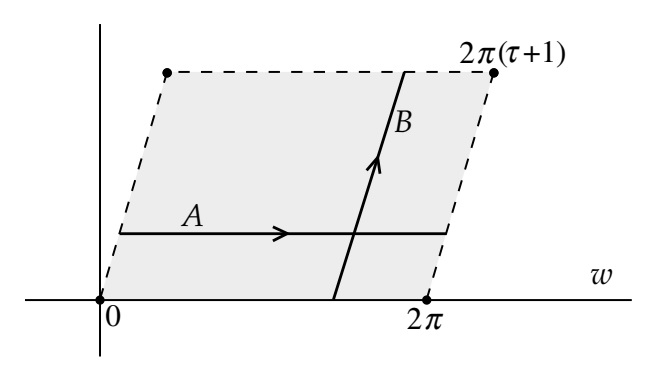
\includegraphics[width=0.5\textwidth]{figure/Fig5.1.jpg}\\
		\caption{Torus with modulus $\tau$, in gauge $d s^{2}=d w d \bar{w}$. The upper and lower edges are identified, as are the right- and left-hand edges. Closed curves $A$ and $B$ are marked for later reference.}\label{Fig5.1}
	\end{center}
\end{figure}

Alternatively, using $\sigma^{a}$, $w=\sigma^{1}+\tau \sigma^{2}$ is defined. The original periodicity is preserved, but the metric takes the more general form \eqref{5.1.9}. The integration over the metric reduces to two integrals over the real and imaginary parts of $\tau$. The metric \eqref{5.1.9} is invariant under complex conjugation and degenerates for real $\tau$, so we can focus our attention on $\operatorname{Im} \tau > 0$. Just as in the circular case \eqref{5.1.5}, we can put these parameters into the metric \eqref{5.1.9} or the periodicity \eqref{5.1.11}. The parameter $\tau$ is called the Teichmüller parameter or, more generally, the modulus.

Unlike the point particle, there is no simple invariant expression for $\tau$ analogous to the invariant length of a circle. There is some additional redundancy that has no analog in the point particle case. The value $\tau+1$ generates the same equivalence set (5.1.11) as $\tau$, replacing $(m, n) \rightarrow(m-n, n)$. The same is true for $-1 / \tau$. Defining $w^{\prime}=\tau w$ and replacing $(m, n) \rightarrow(n,-m)$, repeatedly using these two transformations:
\begin{equation}
	T: \quad \tau^{\prime}=\tau+1, \quad S: \tau^{\prime}=-1 / \tau
\end{equation}
generates:
\begin{equation}
	\tau^{\prime}=\frac{a \tau+b}{c \tau+d}\label{5.1.13}
\end{equation}
where $a, b, c, d$ are integers satisfying $a d-b c=1$.

We can also consider it as follows: the transformation
\begin{equation}
	\left[\begin{array}{l}
		\sigma^{1} \\
		\sigma^{2}
	\end{array}\right]=\left[\begin{array}{ll}
		d & b \\
		c & a
	\end{array}\right]\left[\begin{array}{l}
		\sigma^{\prime 1} \\
		\sigma^{\prime 2}
	\end{array}\right]\label{5.1.14}
\end{equation}
turns the $\sigma$ metric \eqref{5.1.9} into the same form of metric in $\sigma^{\prime}$ but with modulus $\tau^{\prime}$. This is a diffeomorphism mapping of the torus. Since $a d-b c=1$, it is a one-to-one mapping and preserves the periodicity \eqref{5.1.8}. However, it cannot be obtained from a continuous infinitesimal transformation starting from the identity---it is a so-called large coordinate transformation. Curve $A$ in coordinates $\sigma$ maps to a curve in $\sigma^{\prime}$ stretched $a$ times along the $A^{\prime}$ direction and $c$ times along the $B^{\prime}$ direction.

These large coordinate transformations form the group $SL(2, \mathbf{Z})$. The group on the $\tau$ plane is $SL(2, \mathbf{Z}) / \mathbf{Z}_{2} = PSL(2, \mathbf{Z})$, because if the signs of $a, b, c, d$ are all flipped, $\tau^{\prime}$ remains invariant. The group of transformations \eqref{5.1.14} is called the modular group. Using the modular transformation \eqref{5.1.13}, it can be proved that every $\tau$ is equivalent to a point in the region $F_{0}$, as shown in figure (\ref{Fig5.2}).

\begin{figure}[!htbp]
	\begin{center}
		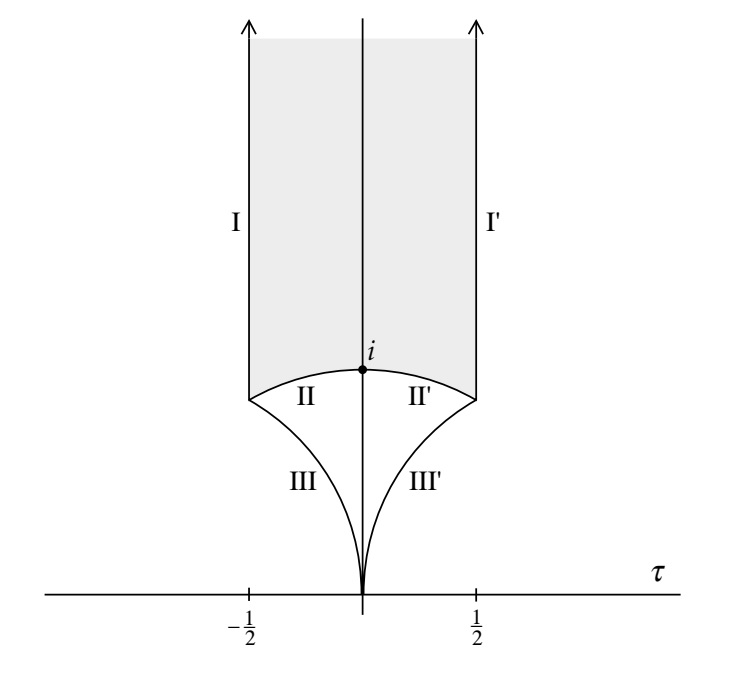
\includegraphics[width=0.5\textwidth]{figure/Fig5.2.jpg}\\
		\caption{The standard fundamental region $F_{0}$ for the moduli space of the torus, shaded. The lines I and I' are identified, as are the arcs II and II'. A different fundamental region, mapped into $F_{0}$ by the modular transformation $S$, is bounded by II, II', III, and III'.}\label{Fig5.2}
	\end{center}
\end{figure}

\begin{equation}
	-\frac{1}{2} \leq \operatorname{Re} \tau \leq \frac{1}{2}, \quad|\tau| \geq 1
\end{equation}
Except for the boundaries identified in the figure, this is called the fundamental region of the upper half-plane modulo $PSL(2, \mathbf{Z})$. Due to the equivalence, $F_{0}$ can be considered rolled up, opening only when $\operatorname{Im} \tau \rightarrow \infty$. The fundamental region $F_{0}$ is a representation of the moduli space of ($\text{diff} \times \text{Weyl}$) inequivalent metrics.

There are further difficulties, as with the point particle. Requiring the metric to take the form (5.1.9) where $\tau$ is in a given fundamental region does not fix all $\text{diff} \times \text{Weyl}$ invariance. The metric and periodicity are invariant under rigid translations:
\begin{equation}
	\sigma^{a} \rightarrow \sigma^{a}+v^{a}
\end{equation}
So this two-parameter $\text{diff} \times \text{Weyl}$ subgroup is not fixed. Additionally, the discrete transformation $\sigma^{a} \rightarrow-\sigma^{a}$ leaves the metric invariant, and in the non-oriented case, $\tau \rightarrow-\bar{\tau}$ via $\left(\sigma^{1}, \sigma^{2}\right) \rightarrow\left(-\sigma^{1}, \sigma^{2}\right)$ also leaves the metric invariant. Thus, there is again a mismatch between metric degrees of freedom and local symmetries: parameters in the metric cannot be removed by symmetry, and symmetry is not fixed by the choice of metric. Unfixed symmetries are called the Conformal Killing Group (CKG).

When there are enough vertex operators in the amplitude, we can completely fix the gauge invariance by fixing the positions of certain vertex operators. On a torus with $n$ vertex operators, the invariance (5.1.16) can be used to fix the position of one vertex operator, leaving the integral over $\tau$ and $n-1$ other positions. The $\mathbf{Z}_{2}$ from $\sigma^{a} \rightarrow-\sigma^{a}$ can be used to fix a second vertex operator in the middle of the torus. In practice, for finite redundancy counts, it is often more convenient to leave some symmetries unfixed and divide by a suitable factor. Additionally, if there are too few vertex operators and some Conformal Killing invariance remains unfixed, then we must explicitly account for the redundancy count.

\subsubsection*{\Large Note to the Reader}
In the remainder of this chapter, we will discuss moduli more generally. The primary goal is the gauge-fixed expression for the string $S$-matrix \eqref{5.3.9}. In fact, most interesting string physics can be seen in tree-level and one-loop amplitudes. For this reason, the measure can be obtained through shortcuts. For tree amplitudes, there are no metric moduli but the positions of certain vertex operators must be fixed. The measure can be reasoned out as explained below \eqref{6.4.4}. For one-loop amplitudes, the measure can be understood in a relatively intuitive way by analogy with the discussion of point particles below \eqref{7.3.9}.

\section{Moduli and Riemann Surfaces}\label{sec:5.2}

Now, we repeat the above discussion in a more general and abstract way. We integrate over all metrics on some given topology $r$. Call this metric space $\mathscr{G}_{r}$. For closed oriented surfaces, we can label $r$ by the number of handles $g$, also called the genus. After accounting for $\text{diff} \times \text{Weyl}$ redundancy, we are left with the moduli space:
\begin{equation}
	\mathscr{M}_{r}=\frac{\mathscr{G}_{r}}{(\text { diff } \times \mathrm{Weyl})_{r}}
\end{equation}
Just as in the torus case, this space is parameterized by a finite number of moduli. For the torus, $\mathscr{M}_{1}$ is the upper half-plane modulo $PSL(2, \mathbf{Z})$, or equivalently any fundamental region such as $F_{0}$. There may also exist a $\text{diff} \times \text{Weyl}$ subgroup, the CKG, that leaves the metric invariant.

When vertex operators are present in the path integral, it is useful to treat their positions on an equal footing with the moduli in the metric. When we need to make a distinction, we will refer to metric moduli. One way to handle the CKG, which is applicable if vertex operators exist in the path integral, is to further specify the gauge by fixing the positions of certain vertex operators. The Polyakov path integral includes an integration over $\mathscr{G}_{r}$ and an integration of $n$ vertex operators over the worldsheet $\mathscr{M}$. The moduli space with vertex operators on topology $r$ is:
\begin{equation}
	\mathscr{M}_{r, n}=\frac{\mathscr{G}_{r} \times M^{n}}{(\text { diff } \times \mathrm{Weyl})_{r}}
\end{equation}
As we saw for the torus, $\operatorname{diff}_{r}$ is generally not connected. Selecting the connected component $\text{diff}_{r 0}$ containing the identity, the quotient
\begin{equation}
	\frac{\operatorname{diff}_{r}}{\operatorname{diff}_{r 0}}
\end{equation}
is the modular group.

It is interesting to study the $\text{diff} \times \text{Weyl}$ redundancy of the metric at the infinitesimal level. That is, searching for metric variations that are not equivalent to a $\text{diff} \times \text{Weyl}$ transformation and are thus equivalent to a change in moduli. We also want to find certain $\text{diff} \times \text{Weyl}$ transformations that do not change the metric; these are the infinitesimal elements of the CKG, called Conformal Killing Vectors (CKVs).

An infinitesimal $\text{diff} \times \text{Weyl}$ transformation changes the metric by:
\begin{equation}
	\delta g_{a b}=-2\left(P_{1} \delta \sigma\right)_{a b}+(2 \delta \omega-\nabla \cdot \delta \sigma) g_{a b}\label{5.2.4}
\end{equation}
where $P_{1}$ is the traceless symmetric linear combination of derivatives (3.3.17). The metric variation $\delta^{\prime} g_{a b}$ corresponding to the moduli is orthogonal to all variations (5.2.4):
\begin{equation}
	\begin{aligned}
		0 &=\int d^{2} \sigma g^{1 / 2} \delta^{\prime} g_{a b}\left[-2\left(P_{1} \delta \sigma\right)^{a b}+(2 \delta \omega-\nabla \cdot \delta \sigma) g^{a b}\right] \\
		&=\int d^{2} \sigma g^{1 / 2}\left[-2\left(P_{1}^{T} \delta^{\prime} g\right)_{a} \delta \sigma^{a}+\delta^{\prime} g_{a b} g^{a b}(2 \delta \omega-\nabla \cdot \delta \sigma)\right]
	\end{aligned}\label{5.2.5}
\end{equation}
where the adjoint is $\left(P_{1}^{T} u\right)_{a}=-\nabla^{b} u_{a b}$.

\begin{tcolorbox}[breakable]
	Note:
	\begin{align*}
		(P_1\delta \sigma)^{a b}&=\frac{1}{2}\left(\nabla^{a} \delta \sigma^{b}+\nabla^{b} \delta \sigma^{a}-g^{a b} \nabla \cdot \delta \sigma\right) \\
		\delta^{\prime} g_{a b}(P_1 \delta \sigma)^{a b}&=\frac{1}{2}\left(\delta^{\prime} g_{a b} \nabla^{a} \delta \sigma^{b}+\delta^{\prime} g_{a b} \nabla^{b} \delta \sigma^{a}-\delta^{\prime} g_{a b} g^{a b} \nabla \cdot \delta \sigma\right)
	\end{align*}
\end{tcolorbox}

In order to make the overlap \eqref{5.2.5} zero for general $\delta \omega$ and $\delta \sigma$, we require
\begin{subequations}
	\begin{equation}
		g^{a b} \delta^{\prime} g_{a b} =0 
	\end{equation}	
	\begin{equation}
		\left(P_{1}^{T} \delta^{\prime} g\right)_{a} =0
	\end{equation}			\label{5.2.6}
\end{subequations}
The first condition requires $\delta^{\prime} g_{a b}$ to be traceless, and it is a traceless symmetric tensor in the kernel of $P_{1}^{T}$. For each solution to these equations, there exists a modulus.

CKVs are those $\delta \sigma$ such that $\delta g_{a b}=0$ in \eqref{5.2.4}. The trace of this equation uniquely determines $\delta \omega$, leaving the Conformal Killing Equation:
\begin{equation}
	\left(P_{1} \delta \sigma\right)_{a b}=0\label{5.2.7}
\end{equation}
Equations \eqref{5.2.6} and (\ref{5.2.7}) become simple for variations around the conformal gauge:
\begin{subequations}
	\begin{equation}
		\partial_{\bar{z}} \delta^{\prime} g_{z z} =\partial_{z} \delta^{\prime} g_{\bar{z} \bar{z}}=0 
	\end{equation}	
	\begin{equation}
		\partial_{\bar{z}} \delta z =\partial_{z} \delta \bar{z}=0
	\end{equation}			\label{5.2.8}
\end{subequations}
Thus, the variation of the moduli corresponds to holomorphic quadratic differentials, and CKVs correspond to holomorphic vector fields. On a torus, the only holomorphic bi-periodic functions are constants, so there are two real moduli and two real CKVs, consistent with the previous section's discussion.

The metric moduli correspond to the kernel of $P_{1}^{T}$ \eqref{5.2.6}, while CKVs correspond to the kernel of $P_{1}$ \eqref{5.2.7}. The Riemann-Roch theorem relates the number of metric moduli $\mu=\operatorname{dim} \operatorname{ker} P_{1}^{T}$ and the number of CKVs $\kappa=\operatorname{dim} \operatorname{ker} P_{1}$ to the Euler number $\chi$:
\begin{equation}
	\mu-\kappa=-3 \chi\label{5.2.9}
\end{equation}
We will derive it later in this chapter. For closed oriented surfaces, $-3 \chi=6 g-6$. This count is for real moduli, splitting complex moduli like $\tau$ into real and imaginary parts.

Furthermore, $\kappa$ is zero for $\chi < 0$, and $\mu$ is zero for $\chi > 0$. To prove this, we cite the following property: one can always find a metric via Weyl transformation such that the scalar curvature $R$ is constant. In this case, $R$ has the same sign as $\chi$. Now, $P_{1}^{T} P_{1}=-\frac{1}{2} \nabla^{2}-\frac{1}{4} R$, so
\begin{equation}
	\begin{aligned}
		\int d^{2} \sigma g^{1 / 2}\left(P_{1} \delta \sigma\right)_{a b}\left(P_{1} \delta \sigma\right)^{a b} &=\int d^{2} \sigma g^{1 / 2} \delta \sigma_{a}\left(P_{1}^{T} P_{1} \delta \sigma\right)^{a} \\
		&=\int d^{2} \sigma g^{1 / 2}\left(\frac{1}{2} \nabla_{a} \delta \sigma_{b} \nabla^{a} \delta \sigma^{b}-\frac{R}{4} \delta \sigma_{a} \delta \sigma^{a}\right)
	\end{aligned}\label{5.2.10}
\end{equation}
For negative $\chi$, the right side is strictly positive definite, so $P_{1} \delta \sigma$ cannot be zero. A similar argument shows that for positive $\chi$, $P_{1}^{T} \delta^{\prime} g$ cannot be zero. Combining these results, we have:
\begin{subequations}
	\begin{equation}
		\chi>0:  \kappa=3 \chi, \quad \mu=0 
	\end{equation}
	\begin{equation}
		\chi<0:  \kappa=0, \quad \mu=-3 \chi
	\end{equation}				\label{5.2.11}		
\end{subequations}

\subsubsection*{\Large Riemann Surfaces}
A common way to describe the moduli space is to choose a metric from each equivalence class, which forms a family of metrics $\hat{g}_{a b}(t ; \sigma)$ depending on moduli $t^{k}$. For the torus, \eqref{5.1.9} gives such a slice. Using the other description \eqref{5.1.11} is often more convenient, where $d w d \bar{w}$ is fixed and the moduli are encoded in the coordinate range. We can formalize this concept as follows.

Recall how a differentiable manifold is defined. A manifold is covered by a set of overlapping charts, where $\sigma_{m}^{a}$ are the coordinates in the $m$-th coordinate chart. When charts $m$ and $n$ overlap, the coordinates in the two charts are related by:
\begin{equation}
	\sigma_{m}^{a}=f_{m n}^{a}\left(\sigma_{n}\right) \label{5.2.12}		
\end{equation}
where transition functions are required to be differentiable. For a Riemannian manifold, each chart is also given a metric $g_{m, a b}\left(\sigma_{m}\right)$, and the values in the overlap region are related by the usual tensor laws.

For a complex manifold, each chart has complex coordinates $z_{m}^{a}$. Transition functions are required to be holomorphic:
\begin{equation}
	z_{m}^{a}=f_{m n}^{a}\left(z_{n}\right)\label{5.2.13}		
\end{equation}
Since holomorphicity does not depend on the coordinates $z_{m}^{a}$ used. Holomorphic functions on the manifold can now be defined. Just as two differentiable manifolds are equivalent if there exists a one-to-one differentiable mapping between them, two complex manifolds are equivalent if there exists a one-to-one holomorphic mapping between them.

In the two-dimensional case (one complex coordinate), the complex manifold is called a Riemann surface. In this case, there is a one-to-one correspondence:
\begin{equation}
	\text{Riemann surfaces} \leftrightarrow \text{Riemannian manifolds mod Weyl}
\end{equation}
We place 'mod Weyl' on the right because 'mod diff' is already implied in the definition of a Riemannian manifold. To see this isomorphism, start from the Riemannian manifold. From our discussion of conformal gauge, we know we can find $z_{m}$ in each chart such that:
\begin{equation}
	d s^{2} \propto d z_{m} d \bar{z}_{m}
\end{equation}
In adjacent charts, coordinates need not be identical, but since $d s^{2} \propto d z_{m} d \bar{z}_{m} \propto d z_{n} d \bar{z}_{n}$, the transition functions are holomorphic. This is a mapping from Riemannian manifolds to two-real-dimensional complex manifolds. For the inverse mapping, one can take metric $d z_{m} d \bar{z}_{m}$ in the $m$-th chart and smooth it in the overlap region to produce a Riemannian manifold. The two characterizations of Riemann surfaces are thus equivalent.

The description of the torus using the complex coordinate $w$ of the parallelogram (\ref{Fig5.1}) illustrates the idea of a complex manifold. Imagine taking a single coordinate chart slightly larger than the basic parallelogram of (\ref{Fig5.1}). The periodicity conditions
\begin{equation}
	w \cong w+2 \pi \cong w+2 \pi \tau
\end{equation}
are the transition functions on the overlap of the two opposite edges of the coordinate chart. These transition functions define the surface. To define the original path integral over the metric, treating the metric as fixed coordinates, such as the square (5.1.7), or at least a fixed set of coordinate charts with fixed transition functions, is the simplest starting point. To study quantum field theory on a given surface, the simplest approach is to handle unit metrics where transition function moduli are related, as in the parallelogram (5.1.11).

One can also see Riemann surfaces as follows. Define the worldsheet as a union of coordinate charts. We can use $\text{diff} \times \text{Weyl}$ degrees of freedom to reach the metric $d z d \bar{z}$ in each chart. Then the gauge choices in the chart overlap can only differ by the $\text{diff} \times \text{Weyl}$ invariance of this metric. This is exactly the conformal transformation we discussed. Thus, Riemann surfaces are the natural place for CFT to grow, because fields in CFT have clear transformation properties under conformal transformations.

\section{The Measure for Moduli}\label{sec:5.3}
We now review the gauge fixing of the Polyakov path integral. We already know that gauge redundancy does not completely eliminate the path integral over the metric, but leaves a finite-dimensional integral over the moduli space. To account for this, it is necessary to refine the discussion of section 3.3.

The path integral for the $S$-matrix is:
\begin{equation}
	\begin{aligned}
		&S_{j_{1} \ldots j_{n}}\left(k_{1}, \ldots, k_{n}\right) \\
		&\quad=\sum_{\text { topologies }} \int \frac{[d \phi d g]}{V_{\text {diff } \times \text { Weyl }}} \exp \left(-S_{\mathrm{m}}-\lambda \chi\right) \prod_{i=1}^{n} \int d^{2} \sigma_{i} g\left(\sigma_{i}\right)^{1 / 2} \mathscr{V}_{j_{i}}\left(k_{i}, \sigma_{i}\right)
	\end{aligned}\label{5.3.1}
\end{equation}
This is the previous expression \eqref{3.5.5}, but now with a universal matter field $c=\tilde{c}=26$, where matter fields are labeled by $\phi$. In gauge fixing, the integration over the metric and positions is replaced by an integration over the gauge group, moduli, and unfixed positions:
\begin{equation}
	[d g] d^{2 n} \sigma \rightarrow[d \zeta] d^{\mu} t d^{2 n-\kappa} \sigma\label{5.3.2}
\end{equation}
After factoring out the gauge volume, the Jacobian of this transformation becomes the measure on the moduli space.

This step is identical to section \ref{sec:3.3}, now accounting for moduli and CKVs. Specifically, the gauge choice now fixes $\kappa$ vertex coordinates, $\sigma_{i}^{a} \rightarrow \hat{\sigma}_{i}^{a}$. Denoting the set of fixed coordinates $(a, i)$ as $f$, define the Faddeev-Popov measure on the moduli space as:
\begin{equation}
	1=\Delta_{\mathrm{FP}}(g, \sigma) \int_{F} d^{\mu} t \int_{\mathrm{diff} \times \mathrm{Weyl}}[d \zeta] \delta\left(g-\hat{g}(t)^{\zeta}\right) \prod_{(a, i) \in f} \delta\left(\sigma_{i}^{a}-\hat{\sigma}_{i}^{\zeta a}\right)\label{5.3.3}
\end{equation}
By definition, each metric $(\text{diff} \times \text{Weyl})$ is equivalent to a $\hat{g}(t)$ for some $t$ and $\zeta$. In fact, as discussed at the end of section \ref{sec:5.1}, there might be a residual discrete symmetry group of finite order $n_{R}$, so the delta function is non-zero at $n_{R}$ points.

Substituting \eqref{5.3.3} into the path integral \eqref{5.3.1} and using the same steps as before gives:
\begin{equation}
	\begin{aligned}
		S_{j_{1} \ldots j_{n}}\left(k_{1}, \ldots, k_{n}\right)=& \sum_{\text {topologies}} \int_{F} d^{\mu} t \Delta_{\mathrm{FP}}(\hat{g}(t), \hat{\sigma}) \int[d \phi] \int \prod_{(a, i) \notin f} d \sigma_{i}^{a} \\	
		&\times \exp \left(-S_{\mathrm{m}}[\phi, \hat{g}(t)]-\lambda \chi\right) \prod_{i=1}^{n}\left[\hat{g}\left(\sigma_{i}\right)^{1 / 2} \mathscr{N}_{j_{i}}\left(k_{i} ; \sigma_{i}\right)\right]
	\end{aligned}\label{5.3.4}
\end{equation}
The integration over metrics and vertex operator coordinates now reduces to an integration over the moduli space $F$ plus unfixed coordinates with the measure given by $\Delta_{\mathrm{FP}}$. In the vertex operators, $\kappa$ positions are fixed.

Now we calculate the Faddeev-Popov measure. The delta function is non-zero at $n_R$ points related by symmetry, so we consider one such point and divide by $n_R$. Expand the definition of $\Delta_{\mathrm{FP}}$ in \eqref{5.3.3} near this point. A general metric variation equals a local symmetry variation plus a change in moduli $t^k$:
\begin{equation}
	\delta g_{a b}=\sum_{k=1}^{\mu} \delta t^{k} \partial_{t^{k}} \hat{g}_{a b}-2\left(\hat{P}_{1} \delta \sigma\right)_{a b}+(2 \delta \omega-\hat{\nabla} \cdot \delta \sigma) \hat{g}_{a b}\label{5.3.5}
\end{equation}
The Faddeev-Popov inverse determinant is:
\begin{equation}
	\begin{aligned}
		\Delta_{\mathrm{FP}}(\hat{g}, \hat{\sigma})^{-1} &=n_{R} \int d^{\mu} \delta t[d \delta \omega d \delta \sigma] \delta\left(\delta g_{a b}\right) \prod_{(a, i) \in f} \delta\left(\delta \sigma^{a}\left(\hat{\sigma}_{i}\right)\right)\\
		&=n_{R}  \int d^{\mu} \delta t d^{\kappa} x\left[d \beta^{\prime} d \delta \sigma\right]  \exp \left[2 \pi i\left(\beta^{\prime}, 2 \hat{P}_{1} \delta \sigma-\delta t^{k} \partial_{k} \hat{g}\right)+2 \pi i \sum_{(a, i) \in f} x_{a i} \delta \sigma^{a}\left(\hat{\sigma}_{i}\right)\right]
	\end{aligned}\label{5.3.6}
\end{equation}
The inner product definition in the second line refers to Exercise 3.2. We followed the same local discussion as in section \ref{sec:3.3}, writing the delta function and functional as integrals over $x$ and $\beta_{ab}$, and integrating over $\delta \omega$ to obtain the constraint that $\beta_{ab}^{\prime}$ is traceless.

As before, replace all bosonic variables with Grassmann variables to convert the integral \eqref{5.3.6}:
\begin{subequations}
	\begin{equation}
		\delta \sigma^{a}  \rightarrow c^{a} 
	\end{equation}
	\begin{equation}
		\beta_{a b}^{\prime}  \rightarrow b_{a b} 
	\end{equation}
	\begin{equation}
		x_{a i}  \rightarrow \eta_{a i} 
	\end{equation}
	\begin{equation}
		\delta t^{k}  \rightarrow \xi^{k}
	\end{equation}
\end{subequations}
Then, under the standard normalization of fields:
\begin{equation}
	\begin{aligned}
		\Delta_{\mathrm{FP}}(\hat{\mathrm{g}}, \hat{\sigma})=& \frac{1}{n_{R}} \int[d b d c] d^{\mu} \xi d^{\kappa} \eta \\
		&\quad \times \exp \left[-\frac{1}{4 \pi}\left(b, 2 \hat{P}_{1} c-\xi^{k} \partial_{k} \hat{g}\right)+\sum_{(a, i) \in f} \eta_{a i} c^{a}\left(\hat{\sigma}_{i}\right)\right] \\
		=& \frac{1}{n_{R}} \int[d b d c] \exp \left(-S_{\mathrm{g}}\right) \prod_{k=1}^{\mu} \frac{1}{4 \pi}\left(b, \partial_{k} \hat{g}\right) \prod_{(a, i) \in f} c^{a}\left(\hat{\sigma}_{i}\right)
	\end{aligned}\label{5.3.8}
\end{equation}
In the last line, we integrated out the Grassmann variables $\eta_{ai}$ and $\xi^k$. The appropriate integration measure on the moduli space is generated by the ghost path integral with this insertion.
\begin{tcolorbox}[breakable]
	\begin{proof}
		We utilise the following identity for $x$ and $y$ $c-$numbers and $\psi$ and $\chi$ grassmann numbers:
		\begin{equation}
			\int_{-\infty}^{\infty} dx \int_{-\infty}^{\infty} dy \, e^{2\pi i \lambda xy} = \frac{1}{\lambda} = \left[ \int d\psi \int d\chi \, e^{\lambda \psi \chi} \right]^{-1}
		\end{equation}
		
		We make the correspondence, including convenient normalisation
		
		\begin{align}
			\delta \sigma^a &\to -\frac{1}{4\pi} c^a \nonumber \\
			\beta'_{ab} &\to b_{ab} \nonumber \\
			x_{ai} &\to \eta_{ai} \nonumber \\
			\delta t^k &\to -\frac{1}{4\pi} \xi^k
		\end{align}
		
		This gives
		
		\begin{equation}
			\Delta_{\text{FB}} = \frac{1}{n_R} \int [db \, dc] \, d^\mu\xi \, d^k \eta \, \exp \left[ -\frac{1}{4\pi} (b, 2\hat{P}_1 c - \xi^k \partial_{t^k} \hat{g}) + \sum_{(a,i) \in f} \eta_{ai} c^a (\hat{\sigma}_i) \right]
		\end{equation}
		
		We can perform the integrations over the Grassmann variables $\xi$ and $\eta$ using $\int d\xi \, e^{\alpha \xi} = \int d\xi \, (1 + \alpha \xi) = \alpha$:
		
		\begin{align}
			\Delta_{\text{FB}} &= \frac{1}{n_R} \int [db \, dc] \exp \left[ -\frac{1}{4\pi} (b, 2\hat{P}_1 c) \right] \prod_{k=1}^\mu \frac{1}{4\pi} (b, \partial_{t^k} \hat{g}) \prod_{(a,i) \in f} c^a (\hat{\sigma}_i) \nonumber \\
			&= \frac{1}{n_R} \int [db \, dc] \exp(-S_g) \prod_{k=1}^\mu \frac{1}{4\pi} (b, \partial_{t^k} \hat{g}) \prod_{(a,i) \in f} c^a (\hat{\sigma}_i)
		\end{align}
		
		where we have used the definition of the ghost action \eqref{3.3.21}
		
		\begin{equation}
			S_g = \frac{1}{2\pi} \int d^2 \sigma \sqrt{\hat{g}} \, b_{ab} (\hat{P}_1 c)^{ab} = \frac{1}{2\pi} (b, \hat{P}_1 c)
		\end{equation}
	\end{proof}
\end{tcolorbox}
We do not attempt to keep track of the overall sign in intermediate steps; since this is a Jacobian, we can implicitly choose the overall sign to yield a positive result. The complete expression for the $S$-matrix is:
\begin{equation}
	\begin{aligned}
		&S_{j_{1} \ldots j_{n}}\left(k_{1}, \ldots, k_{n}\right)\\
		&=\sum_{\text {topologies }} \int_{F} \frac{d^{\mu} t}{n_{R}} \int[d \phi d b d c] \exp \left(-S_{\mathrm{m}}-S_{\mathrm{g}}-\lambda \chi\right) \\
		&\times \prod_{(a, i) \notin f} \int d \sigma_{i}^{a} \prod_{k=1}^{\mu} \frac{1}{4 \pi}\left(b, \partial_{k} \hat{g}\right) \prod_{(a, i) \in f} c^{a}\left(\hat{\sigma}_{i}\right) \prod_{i=1}^{n} \hat{g}\left(\sigma_{i}\right)^{1 / 2} \mathscr{V}_{j_{i}}\left(k_{i}, \sigma_{i}\right)
	\end{aligned}\label{5.3.9}
\end{equation}
This result is ready to be extended to all bosonic string theories—closed or open, oriented or non-oriented—the only difference being what topologies to include and what vertex operators to allow. Eq. \eqref{5.3.9} is a useful and beautiful result. The complexities introduced by moduli and CKVs are accounted for by inserting $b$ and $c$ into the path integral. For each fixed coordinate, $d \sigma_{i}^{a}$ is replaced by $c_{i}^{a}$, and each metric modulus gives a $b$ insertion.

\subsubsection*{\Large Representation in Determinant Form}
In \eqref{5.3.8}, we expressed the Faddeev-Popov determinant as an integral over Grassmann variables and fields. We now want to simplify it into a product of finite-dimensional functional determinants. As we continue to study the string $S$-matrix in the following chapters, this direct path integral approach is only one of the methods we will use.

Expand the ghost fields in a suitable complete basis:
\begin{equation}
	c^{a}(\sigma)=\sum_{J} c_{J} \mathrm{C}_{J}^{a}(\sigma), \quad b_{a b}(\sigma)=\sum_{K} b_{K} \mathrm{~B}_{K a b}(\sigma)
\end{equation}
The complete bases $\mathrm{C}_{J}^{a}$ and $\mathrm{B}_{K a b}$ are defined as follows. The derivative $P_{1}$ appearing in the ghost action converts a vector into a traceless symmetric tensor. Its transpose performs the opposite function. 
\begin{tcolorbox}[breakable]
	\begin{remark}
		We expand the ghost fields in a complete set of eigenfunctions of the operators $P_1$ and $P_1^\dagger$. For the $c$ ghost we write
		\begin{align}
			c^{a}(\sigma) = \sum_{j=1}^{\kappa} c_{0j} \, C_{0j}^{a}(\sigma) \;+\; \sum_{J=1}^{\infty} c_{J} \, C_{J}^{a}(\sigma),
		\end{align}
		where the $C_{0j}$ are the \textbf{zero modes} satisfying $P_1 C_{0j} = 0$ (the conformal Killing vectors), and the $C_{J}$ are the \textbf{nonzero modes} with $P_1 C_{J} = \nu_J B_J \neq 0$.
		
		Similarly, for the $b$ ghost we have
		\begin{align}
			b_{ab}(\sigma) = \sum_{k=1}^{\mu} b_{0k} \, B_{0k\,ab}(\sigma) \;+\; \sum_{K=1}^{\infty} b_{K} \, B_{K\,ab}(\sigma),
		\end{align}
		where the $B_{0k}$ are the \textbf{zero modes} satisfying $P_1^\dagger B_{0k} = 0$, and the $B_{K}$ are the nonzero modes with $P_1^\dagger B_K = \nu_K C_K$. The zero modes $c_{0j}$ and $b_{0k}$ do \textbf{not} appear in $S_g$ because $P_1 C_{0j}=0$ and $(B_{0k}, P_1 c)=0$.
	\end{remark}
\end{tcolorbox}
The ghost action can be written as:
\begin{equation}
	S_{\mathrm{g}}=\frac{1}{2 \pi}\left(b, P_{1} c\right)=\frac{1}{2 \pi}\left(P_{1}^{T} b, c\right)\label{5.3.11}
\end{equation}
\begin{tcolorbox}[breakable]
	\begin{remark}
		We need to write the ghost action in terms of the ghost Eigenfunctions. From \eqref{5.3.11} and
		\eqref{5.3.15} we have
		\begin{align}
			S_g &= \frac{1}{2\pi} (b, P_1 c) = \frac{1}{2\pi} \left( \sum_{k=1}^\mu b_{0k} B_{0k} + \sum_K b_K B_K, \sum_{j=1}^\kappa c_{0j} P_1 C_{0j} + \sum_J c_J P_1 C_J \right) \nonumber \\
			\intertext{But we know that $P_1 C_{0j} = 0$ and that similarly $P_1^T B_{0k} = 0$. There is thus only one combination that survives}
			S_g &= \frac{1}{2\pi} \sum_{J,K} b_K c_J (B_K, P_1 C_J) = \frac{1}{2\pi} \sum_{J,K} b_K c_J \left( \frac{1}{\nu_K} P_1 C_K, P_1 C_J \right) \nonumber \\
			&= \frac{1}{2\pi} \sum_{J,K} \frac{b_K c_J}{\nu_K} (C_K, P_1^T P_1 C_J) = \frac{1}{2\pi} \sum_{J,K} \frac{b_K c_J}{\nu_K} (C_K, \nu_J^2 C_J) = \frac{1}{2\pi} \sum_J \nu_J b_J c_J
		\end{align}
	\end{remark}
\end{tcolorbox}
We cannot diagonalize $P_{1}$ in a $\text{diff}$-invariant way because it converts one type of field into another, but we can diagonalize $P_{1}^{T} P_{1}$ and $P_{1} P_{1}^{T}$:
\begin{equation}
	P_{1}^{T} P_{1} \mathrm{C}_{J}^{a}=v_{J}^{\prime 2} \mathrm{C}_{J}^{a}, \quad P_{1} P_{1}^{T} \mathrm{~B}_{K a b}=v_{K}^{2} \mathrm{~B}_{K a b}
\end{equation}
The eigenfunctions can be chosen to be real and normalized in the following inner products:
\begin{subequations}
	\begin{equation}
		\left(\mathrm{C}_{J}, \mathrm{C}_{J^{\prime}}\right) =\int d^{2} \sigma g^{1 / 2} \mathrm{C}_{J}^{a} \mathrm{C}_{J^{\prime} a}=\delta_{J J^{\prime}} 
	\end{equation}
	\begin{equation}
		\left(\mathrm{B}_{K}, \mathrm{~B}_{K^{\prime}}\right) =\int d^{2} \sigma g^{1 / 2} \mathrm{~B}_{K a b} \mathrm{~B}_{K^{\prime}}^{a b}=\delta_{K K^{\prime}}
	\end{equation}
\end{subequations}
Now note that:
\begin{equation}
	\left(P_{1} P_{1}^{T}\right) P_{1} \mathrm{C}_{J}=P_{1}\left(P_{1}^{T} P_{1}\right) \mathrm{C}_{J}=v_{J}^{\prime 2} P_{1} \mathrm{C}_{J}
\end{equation}
So $P_{1} \mathrm{C}_{J}$ is an eigenfunction of $P_{1} P_{1}^{T}$. In the same way, $P_{1}^{T} \mathrm{~B}_{K}$ is an eigenfunction of $P_{1}^{T} P_{1}$. Therefore, unless $P_{1} \mathrm{C}_{J}=0$ or $P_{1}^{T} \mathrm{~B}_{K}=0$, there exists a one-to-one mapping between the eigenfunctions $(C_J\leftrightarrow B_J)$. This paring fails if the eigenfunction correspond to zero eigenvalues i.e. $P_{1}^{T} P_{1}C=0$ or $P_{1} P_{1}^{T}C=0$. They are precisely the CKVs $(\in \ker P_1)$ and holomorphic quadratic differentials $(\in \ker P^{T}_1)$, and their numbers are $\kappa$ and $\mu$, respectively.

We denote the \textbf{zero-eigenvalue eigenfunctions} of $P_{1}^{T} P_{1}$ or $P_{1} P_{1}^{T}$ as $\mathrm{C}_{0 j}$ or $\mathrm{B}_{0 k}$, and non-zero eigenvalues are labeled $J, K=1, \ldots$. For the latter, the normalization of the associated functions is:
\begin{equation}
	\mathrm{B}_{J a b}=\frac{1}{v_{J}}\left(P_{1} \mathrm{C}_{J}\right)_{a b}, \quad v_{J}=v_{J}^{\prime} \neq 0\label{5.3.15}
\end{equation}
\begin{tcolorbox}[breakable]
	\begin{proof}
		For those Eigenfunctions \( B_J \) and \( C_J \) that have equal but non zero Eigenvalue \( \nu_J = \nu'_J \), we have the normalisation
		
		\begin{align}
			(B_J, B_{J'}) &= \frac{1}{\nu_J \nu_{J'}} (P_1 C_J, P_1 C_{J'}) = \frac{1}{\nu_J \nu_{J'}} (C_J, P_1^T P_1 C_{J'}) \nonumber \\
			&= \frac{1}{\nu_J \nu_{J'}} (C_J, \nu_J^2 C_{J'}) = \frac{\nu_J}{\nu_J} (C_J, C_{J'}) = \frac{\nu_J}{\nu_J} \delta_{J,J'} = \delta_{J,J'}
		\end{align}
	\end{proof}
\end{tcolorbox}
In this basis, the ghost path integral $\Delta_{\mathrm{FP}}$ from \eqref{5.3.8} becomes:
\begin{equation}
	\int \prod_{k=1}^{\mu} d b_{0 k} \prod_{j=1}^{k} d c_{0 j} \prod_{J} d b_{J} d c_{J} \exp \left(-\frac{v_{J} b_{J} c_{J}}{2 \pi}\right) \prod_{k^{\prime}=1}^{\mu} \frac{1}{4 \pi}\left(b, \partial_{k^{\prime}} \hat{g}\right) \prod_{(a, i) \in f} c^{a}\left(\sigma_{i}\right)
\end{equation}
\begin{tcolorbox}[breakable]
	\begin{remark}
		The path integral includes the insertions
		\begin{align}
			\prod_{k=1}^{\mu} \frac{1}{4\pi} \bigl(b, \partial_k \hat{g}\bigr) \prod_{(a,i)\in f} c^{a}(\hat{\sigma}_i).
		\end{align}
		Here $f$ is the set of vertex coordinates we can fix, which is equal to the number of conformal Killing vectors, i.e. $\kappa$.
		\begin{itemize}
			\item The factor $\prod_k (b, \partial_k \hat{g})$ picks out the \textbf{zero modes of $b$} because $\partial_k \hat{g}$ is orthogonal to all nonzero $B_K$. Hence
			\begin{align}
				(b, \partial_k \hat{g}) = \sum_{k'=1}^{\mu} b_{0k'} (B_{0k'}, \partial_k \hat{g}).
			\end{align}
			\item The factor $\prod_{(a,i)} c^{a}(\hat{\sigma}_i)$ includes contributions from both zero and nonzero modes of $c$:
			\begin{align}
				c^{a}(\hat{\sigma}_i) = \sum_{j=1}^{\kappa} c_{0j} C_{0j}^{a}(\hat{\sigma}_i) + \sum_{J} c_{J} C_{J}^{a}(\hat{\sigma}_i).
			\end{align}
			\item  The nonzero modes \(c_J\) do \textbf{not} contribute to the final result.  
			Consider a single nonzero mode pair \((b_J, c_J)\) with an insertion of \(c_J\).  
			The relevant integral is
			\begin{align*}
				\int db_J \, dc_J \; e^{-\frac{\nu_J}{2\pi} b_J c_J} \; c_J C_J^a(\sigma)=0
			\end{align*}
			because the exponential expands to \(1 - \frac{\nu_J}{2\pi} b_J c_J\), and the term \(1 \cdot c_J\) gives \(\int db_J dc_J \, c_J = 0\) (odd Grassmann integral), while the term \(b_J c_J \cdot c_J\) vanishes since \(c_J^2 = 0\).  
			More generally, any insertion containing an odd number of \(c_J\) factors yields zero, and an insertion with no \(c_J\) factors gives a nonzero constant.  
			Thus, to obtain a nonvanishing result from the product \(\prod_{(a,i)} c^a(\hat{\sigma}_i)\), only the \textbf{zero modes} \(c_{0j}\) can appear; the nonzero mode terms \(c_J C_J^a(\hat{\sigma}_i)\) drop out completely after integration.
		\end{itemize}			
	\end{remark}
\end{tcolorbox}
From section A.2, we know that unless a variable appears in the integrand, the Grassmann integral is zero. $c_{0 j}$ and $b_{0 k}$ do not appear in the action, but only in the insertions. In fact, the number of each type of insertion in the integral (5.3.16), $\kappa$ and $\mu$, matches the ghost zero modes respectively. We have exactly enough insertions to give a non-zero result, and in the insertions, only the zero-mode part of the ghost fields contributes. Therefore:
\begin{equation}
	\begin{aligned}
		\Delta_{\mathrm{FP}}=\int \prod_{k=1}^{\mu} & d b_{0 k} \prod_{k^{\prime}=1}^{\mu}\left[\sum_{k^{\prime \prime}=1}^{\mu} \frac{b_{0 k^{\prime \prime}}}{4 \pi}\left(\mathrm{B}_{0 k^{\prime \prime}}, \partial_{k^{\prime}} \hat{g}\right)\right] \int \prod_{j=1}^{\kappa} d c_{0 j} \prod_{(a, i) \in f}\left[\sum_{j^{\prime}=1}^{\kappa} c_{0 j^{\prime}} \mathrm{C}_{0 j^{\prime}}^{a}\left(\sigma_{i}\right)\right] \\
		& \times \int \prod_{J} d b_{J} d c_{J} \exp \left(-\frac{v_{J} b_{J} c_{J}}{2 \pi}\right)
	\end{aligned}
\end{equation}
Summing over all ways to fill the Grassmann variables in the zero-mode integrals, in each case, the integral generates a finite determinant, and the non-zero modes produce an infinite product, a functional determinant. Combined:
\begin{equation}
	\Delta_{\mathrm{FP}}=\operatorname{det} \frac{\left(\mathrm{B}_{0 k}, \partial_{k^{\prime}} \hat{g}\right)}{4 \pi} \operatorname{det} \mathrm{C}_{0 j}^{a}\left(\sigma_{i}\right) \operatorname{det}^{\prime}\left(\frac{P_{1}^{T} P_{1}}{4 \pi^{2}}\right)^{1 / 2}
\end{equation}
Note that $\mathrm{C}_{0 j}^{a}\left(\sigma_{i}\right)$ is a square matrix, where $(a, i) \in f$ ranges over $\kappa$ values like $j$. The prime on the functional determinant indicates that the zero eigenvalues are removed.

\subsubsection*{\Large Riemann-Roch Theorem}
We now give a path integral derivation of the Riemann-Roch theorem. For the ghost current of the holomorphic $bc$ system (no $\tilde{b}, \tilde{c}$), the current conservation anomaly derived in Exercise 3.6 is:
\begin{equation}
	\nabla_{a} j^{a}=\frac{1-2 \lambda}{4} R
\end{equation}
Noether's theorem relates current conservation to invariance. For a non-conserved current, the discussion found:
\begin{equation}
	\frac{\delta([d \phi] \exp (-S))}{[d \phi] \exp (-S)}=\frac{i \epsilon}{2 \pi} \int d^{2} \sigma g^{1 / 2} \nabla_{a} j^{a} \rightarrow-i \epsilon \frac{2 \lambda-1}{2} \chi
\end{equation}
The ghost number symmetry acts as $\delta b = -i \epsilon b, \delta c = i \epsilon c$. When the path integral is non-zero, the transformations of the measure, action, and insertions must cancel each other. Thus, from the anomaly, we learn that the number of $c$ insertions minus the number of $b$ insertions is $3\chi/2$. The path integral calculation relates the number of insertions to the number of zero modes, thus giving the same difference:
\begin{equation}
	\frac{1}{2}(\kappa-\mu)=\frac{1}{2}\left(\operatorname{dim} \operatorname{ker} P_{1}-\operatorname{dim} \operatorname{ker} P_{1}^{T}\right)
\end{equation}
The factor of $1/2$ appears because we only considered the holomorphic theory; the anti-holomorphic theory gives the same contribution. Equating the result from the anomaly with the result from the zero modes gives the Riemann-Roch theorem $\kappa-\mu=3\chi$. For a general $bc$ system, the same method will find:
\begin{equation}
	\operatorname{dim} \operatorname{ker} P_{n}-\operatorname{dim} \operatorname{ker} P_{n}^{T}=(2 n+1) \chi
\end{equation}
where the $P_n$ operator is defined in Exercise 3.2.

\section{More about the measure}
Here we collect some general properties of gauge-fixed string amplitudes. They play a foundational role in the more formal investigations in Chapter \ref{cha:9}.

\subsubsection*{\Large Gauge Invariance}
The gauge-fixed amplitudes generated by the Faddeev-Popov treatment are BRST-invariant and independent of the gauge choice. However, it is useful to explicitly check whether it has all the expected properties.

First, it is independent of the choice of coordinates $t$ on the moduli space. For new coordinates $t^{\prime k}(t)$:
\begin{equation}
	\begin{aligned}
		d^{\mu} t^{\prime} &=\left|\operatorname{det} \frac{\partial t^{\prime}}{\partial t}\right| d^{\mu} t \\
		\prod_{k=1}^{\mu} \frac{1}{4 \pi}\left(b, \partial_{k}^{\prime} \hat{g}\right) &=\operatorname{det}\left(\frac{\partial t}{\partial t^{\prime}}\right) \prod_{k=1}^{\mu} \frac{1}{4 \pi}\left(b, \partial_{k} \hat{g}\right)
	\end{aligned}
\end{equation}
And these two Jacobians cancel each other out (up to a sign, which we manually fix to give a positive measure). In other words, the integral induced by the $b$ ghost transforms like a density on the moduli space.

Second, let us see that the measure is invariant under Weyl transformations of the gauge slice. Under a Weyl transformation:
\begin{equation}
	\delta \hat{g}_{a b}^{\prime}(t ; \sigma)=2 \delta \omega(t ; \sigma) \hat{g}_{a b}(t ; \sigma)
\end{equation}
The variation of the action and measure produces an insertion of the local operator $T_a^a$, which is zero for $D=26$ due to the equations of motion. Thus, we only need to worry about the effects on the individual insertions. Vertex operator insertions are zero due to contractions. The insertion of $c^a(\sigma_i)$ is zero according to the discussion below (3.3.24). For:
\begin{equation}
	\begin{aligned}
		\left(b, \partial_{k} \hat{g}^{\prime}\right) &=\int d^{2} \sigma \hat{g}^{\prime 1 / 2} b_{a b} \hat{g}^{\prime a c} \hat{g}^{b d} \partial_{k} \hat{g}_{c d}^{\prime} \\
		&=\int d^{2} \sigma \hat{g}^{1 / 2} b_{a b}\left(\hat{g}^{a c} \hat{g}^{b d} \partial_{k} \hat{g}_{c d}+2 \hat{g}^{a b} \partial_{k} \omega\right) \\
		&=\left(b, \partial_{k} \hat{g}\right)
	\end{aligned}
\end{equation}
The last equality holds due to the tracelessness of $b$.

Third, we check the invariance under infinitesimal $\text{diff}$ transformations $\delta \sigma = \xi(t; \sigma)$. Extension to general $\text{diff}$ transformations is direct. In the amplitude \eqref{5.3.9}, the only terms that are not immediately invariant are the $b$ insertions and the vertex operators with fixed coordinates. The former transforms as:
\begin{equation}
	\begin{aligned}
		\delta\left(b, \partial_{k} \hat{g}\right) &=-2\left(b, P_{1} \partial_{k} \xi\right) \\
		&=-2\left(P_{1}^{T} b, \partial_{k} \xi\right) \\
		&=0
	\end{aligned}
\end{equation}
where the equations of motion for $b$ are used. The $b$ equations of motion come from $\delta S / \delta c = 0$, so source terms will exist on the $c$ insertions; they are needed to explain the effect of coordinate transformations on the fixed vertex operators.

\subsubsection*{\Large BRST Invariance}
We now prove the full BRST invariance of \eqref{5.3.9}. From the local analysis, we know that the path integral measure and action are invariant, so we must examine the effect of BRST transformations on the insertions. In the gauge-fixed path integral (5.3.9), fixed vertex operators are accompanied by a factor of $c$ or $\tilde{c} c$. This is our description of the BRST-invariant vertex operators corresponding to OCQ states at the end of section \ref{sec:4.4}.

On the other hand, integrated vertex operators are not BRST-invariant; they have the BRST property:
\begin{equation}
	\delta_{\mathrm{B}} \mathscr{V}_{\mathrm{m}}=i \epsilon \partial_{a}\left(c^{a} \mathscr{V}_{\mathrm{m}}\right)
\end{equation}
which is zero in the integral sense. Finally, there is the variation of the $b$ insertion:
\begin{equation}
	\delta_{\mathrm{B}}\left(b, \partial_{k} \hat{g}\right)=i \epsilon\left(T, \partial_{k} \hat{g}\right)
\end{equation}
The insertion of the energy-momentum tensor only produces a derivative with respect to $t^{k}$, so the BRST variation is zero except for a term that might come from the boundary of the moduli space. We will examine the boundary of the moduli space in the next chapter. In most cases, there is no surface contribution, which is due to the so-called "canceling propagator" argument. In certain situations, this argument does not apply, and we will see how to handle this.

Importantly, the gauge-fixed result \eqref{5.3.9} can be written directly from the requirement of BRST invariance without referring to the gauge-fixed form. As we saw when calculating the path integral, there exist at least $\mu$ $b$ insertions and $\kappa$ $c$ insertions, otherwise the path integral is zero. In the amplitude \eqref{5.3.9}, there are exactly the correct number of ghost insertions to give a non-zero result. Once we introduce the necessary $b$ factors, the BRST transformation brings a convolution with the $t^{k}$ derivative of the metric in the energy-momentum tensor. This is proportional to the derivative with respect to the moduli, so just as we did before, integrating over the moduli space yields an invariant result.

The result \eqref{5.3.9} can be generalized in various ways (e.g., the Conformal Killing invariant case is kept unfixed). In Chapter \ref{cha:7}, for the torus without vertex operators, we will explicitly exemplify this point. BRST invariance implies that the amplitudes of BRST-equivalent states are the same. If we add a null part $Q_{B}|\chi\rangle$ to any state, the effect is to insert the variation $\delta_{B} \mathscr{V}_{\chi}$ into the path integral; this integral is zero. This is important because the physical Hilbert space is equivalent to the cohomology, so equivalent states should have the same amplitude.

\subsubsection*{\Large The Measure for Riemann Surfaces}
We derived the Faddeev-Popov measure in the framework where the gauge-fixed worldsheet is derived from a moduli-dependent metric. We now recast this result in the framework of Riemann surfaces, where the structure is encoded into moduli-dependent transition functions.

To express the value of the measure at a given point $t_{0}$ in the moduli space, we take a set of coordinate charts, where the $m$-th coordinate chart has complex coordinate $z_{m}$, and holomorphic transition functions, where the metric $\hat{g}\left(t_{0}\right)$ in each coordinate chart is equivalent to $d z_{m} d \bar{z}_{m}$. Now consider the change in moduli. We first describe it as a transformation in a metric with fixed transition functions, and then convert it into a transformation of transition functions with a fixed metric.

In the first description, define the Beltrami differential:
\begin{equation}
	\mu_{k a}^{b}=\frac{1}{2} \hat{g}^{b c} \partial_{k} \hat{g}_{a c}\label{5.4.7}
\end{equation}
The $b$ insertion for $\delta t^{k}$ becomes:
\begin{equation}
	\frac{1}{2 \pi}\left(b, \mu_{k}\right)=\frac{1}{2 \pi} \int d^{2} z\left(b_{z z} \mu_{k \bar{z}}^{z}+b_{\bar{z} \bar{z}} \mu_{k z}^{\bar{z}}\right)\label{5.4.8}
\end{equation}
\begin{tcolorbox}[breakable]
	\begin{proof}
		\begin{align}
			\frac{1}{2\pi}(b,\mu_k)
			&= \frac{1}{2\pi} \int d^2\sigma \sqrt{g}\, b_{ab}\,\mu_k^{ab}
			= \frac{1}{2\pi} \int d^2\sigma \sqrt{g}\, b_{ab}\, g^{ac}\,\mu_{kc}^{\ \ b}\nonumber \\
			&= \frac{1}{2\pi} \int d^2\sigma \sqrt{g}\, b_{ab}\, \hat g^{ac}\,\frac{1}{2}\hat g^{bd}\,\partial_k \hat g_{cd}
			= \frac{1}{4\pi} \int d^2\sigma \sqrt{g}\, b^{cd}\,\partial_k \hat g_{cd}\nonumber \\
			&= \frac{1}{4\pi} \int d^2\sigma \sqrt{g}\, b_{cd}\,\partial_k \hat g^{cd}
			= \frac{1}{4\pi} (b, \partial_k \hat g)
		\end{align}
		
		which is the $b$ insertion. In complex coordinates in the conformal gauge this becomes
		
		\begin{align}
			\frac{1}{2\pi}(b,\mu_k)
			&= \frac{1}{2\pi} \int d^2\sigma \sqrt{g}\, b_{ab}\,\hat g^{ac}\,\mu_{kc}^{\ \ b}\nonumber \\
			&= \frac{1}{2\pi} \int \frac{1}{2} d^2 z \left(
			b_{zz}\,\hat g^{z\bar z}\,\mu_{k\bar z}^{\ \ z}
			+ b_{\bar z\bar z}\,\hat g^{\bar z z}\,\mu_{k z}^{\ \ \bar z}
			\right) \nonumber\\
			&= \frac{1}{2\pi} \int d^2 z \left(
			b_{zz}\,\mu_{k\bar z}^{\ \ z}
			+ b_{\bar z\bar z}\,\mu_{k z}^{\ \ \bar z}
			\right)
		\end{align}
		QED.
	\end{proof}
\end{tcolorbox}
In the second description, after the transformation $\delta t^{k}$ in the moduli, there will be new coordinates in each chart:
\begin{equation}
	z_{m}^{\prime}=z_{m}+\delta t^{k} v_{k m}^{z_{m}}\left(z_{m}, \bar{z}_{m}\right)\label{5.4.9}
\end{equation}
The superscript on $v_{k m}^{a}$ is a vector index; note that $v_{k m}^{a}$ is only defined in the $m$-th coordinate chart. By the definition of Riemann surfaces, $d z_{m}^{\prime} d \bar{z}_{m}^{\prime}$ is equivalent to the metric at $t_{0}+\delta t$:
\begin{equation}
	d z_{m}^{\prime} d \bar{z}_{m}^{\prime} \propto d z_{m} d \bar{z}_{m}+\delta t^{k}\left(\mu_{k z_{m}}^{\bar{z}_{m}} d z_{m} d z_{m}+\mu_{k \bar{z}_{m}}^{z_{m}} d \bar{z}_{m} d \bar{z}_{m}\right)\label{5.4.10}
\end{equation}
\begin{tcolorbox}[breakable]
	\begin{proof}
		We keep the coordinate system fixed, but change the moduli by an infinitesimal amount $t^k\to t^k+\delta t^k$ and suppressing the subscript $m$ for clarity:
		\begin{align}
			g &\propto 2g_{z\bar z}(t)\,dz\,d\bar z + g_{zz}(t)\,dz\,dz + g_{\bar z\bar z}(t)\,d\bar z\,d\bar z \nonumber\\
			&\to 2g_{z\bar z}(t+\delta t)\,dz\,d\bar z + g_{zz}(t+\delta t)\,dz\,dz + g_{\bar z\bar z}(t+\delta t)\,d\bar z\,d\bar z \nonumber\\
			&= 2\big[g_{z\bar z}(t) + \partial_k g_{z\bar z}(t)\,\delta t^k\big] dz\,d\bar z \notag \\
			&\quad + \big[g_{zz}(t) + \partial_k g_{zz}(t)\,\delta t^k\big] dz\,dz
			+ \big[g_{\bar z\bar z}(t) + \partial_k g_{\bar z\bar z}(t)\,\delta t^k\big] d\bar z\,d\bar z\nonumber \\
			&= \big[1 + 2\partial_k g_{z\bar z}(t)\,\delta t^k\big] dz\,d\bar z 
			+ \delta t^k \big[\partial_k g_{zz}(t)\,dz\,dz + \partial_k g_{\bar z\bar z}(t)\,d\bar z\,d\bar z\big] \nonumber\\
			&= dz\,d\bar z + \delta t^k \big[\partial_k g_{zz}(t)\,dz\,dz + \partial_k g_{\bar z\bar z}(t)\,d\bar z\,d\bar z\big]\label{5.105}
		\end{align}
		
		where we have kept the lowest order in each metric component. Let us now look at the Beltrami differentials. Using the definition \eqref{5.4.7} we have
		\begin{align}
			\mu_{k\,\bar z}^{\ \ z} &= \frac{1}{2}\hat g^{z\bar z}\,\partial_k \hat g_{\bar z\bar z}
			= \partial_k \hat g_{\bar z\bar z}, \nonumber\\
			\mu_{k\,z}^{\ \ \bar z} &= \frac{1}{2}\hat g^{z\bar z}\,\partial_k \hat g_{zz}
			= \partial_k \hat g_{zz}
		\end{align}
		
		and thus
		\begin{align}
			g \propto dz\,d\bar z + \delta t^k \left[
			\mu_{k\,\bar z}^{\ \ z}\,dz\,dz
			+ \mu_{k\,z}^{\ \ \bar z}\,d\bar z\,d\bar z
			\right]
		\end{align}
		QED.
	\end{proof}
\end{tcolorbox}
Therefore, the relation between the coordinate change $v_{k m}^{a}$ and the Beltrami differential is:
\begin{equation}
	\mu_{k z_{m}}^{\bar{z}_{m}}=\partial_{z_{m}} v_{k m}^{\bar{z}_{m}}, \quad \mu_{k \bar{z}_{m}}^{z_{m}}=\partial_{\bar{z}_{m}} v_{k m}^{z_{m}}\label{5.4.11}
\end{equation}
This is the infinitesimal version of the Beltrami equation. It implies that $v_{k m}^{z_{m}}$ is not holomorphic, otherwise it would not correspond to a change in moduli. Additionally, there is a holomorphic part in $v_{k m}^{z_{m}}$ not determined by the Beltrami equation, and an anti-holomorphic part for $v_{k m}^{\bar{z}_{m}}$; these correspond to the degrees of freedom for performing holomorphic reparameterizations in each chart.
\begin{tcolorbox}
	\begin{proof}
		From \eqref{5.4.9},
		\[
		z' = z + \delta t^k v_k^z,
		\]
		we have
		\begin{align}
			dz' = dz + \delta t^k \left( \partial_z v_k^z\, dz + \partial_{\bar z} v_k^z\, d\bar z \right)
		\end{align}
		
		and thus
		\begin{align}
			dz\,d\bar z' 
			&= \left[ dz + \delta t^k \left( \partial_z v_k^z\, dz + \partial_{\bar z} v_k^z\, d\bar z \right) \right]
			\left[ d\bar z + \delta t^k \left( \partial_{\bar z} v_k^{\bar z}\, d\bar z + \partial_z v_k^{\bar z}\, dz \right) \right] \notag \\
			&= dz\,d\bar z 
			+ \delta t^k \Big( \partial_z v_k^{\bar z}\, dz\,dz 
			+ \partial_{\bar z} v_k^z\, d\bar z\,d\bar z 
			+ \partial_z v_k^z\, dz\,d\bar z 
			+ \partial_{\bar z} v_k^{\bar z}\, dz\,d\bar z \Big) \notag \\
			&= dz\,d\bar z 
			+ \delta t^k \Big( \partial_z v_k^{\bar z}\, dz\,dz 
			+ \partial_{\bar z} v_k^z\, d\bar z\,d\bar z \Big)
		\end{align}
		
		where, just as in \eqref{5.105}, we have ignored the $dz\,d\bar z$ contribution. Comparing this with \eqref{5.4.10} we find
		\begin{align}
			\mu_{k\,\bar z m}^{\ \ \ z m} &= \partial_{\bar z_m} v_{k m}^{z m},
			\qquad
			\mu_{k\,z m}^{\ \ \ \bar z m} = \partial_{z_m} v_{k m}^{\bar z m}
		\end{align}
	\end{proof}
\end{tcolorbox}
Integrating by parts, the $b$ insertion \eqref{5.4.8} becomes:
\begin{equation}
	\frac{1}{2 \pi}\left(b, \mu_{k}\right)=\frac{1}{2 \pi i} \sum_{m} \oint_{C_{m}}\left(d z_{m} v_{k m}^{z_{m}} b_{z_{m} z_{m}}-d \bar{z}_{m} v_{k m}^{\bar{z}_{m}} b_{\bar{z}_{m} \bar{z}_{m}}\right)\label{5.4.12}
\end{equation}
The contour $C_{m}$ surrounds the $m$-th coordinate chart counter-clockwise. 
\begin{tcolorbox}[breakable]
	\begin{proof}
	Using \eqref{5.4.11} in \eqref{5.4.8} we have
	\begin{align}
		\frac{1}{2\pi}(b,\mu_k)
		&= \frac{1}{2\pi} \int d^2 z \left( b_{zz}\,\partial_{\bar z} v_k^z + b_{\bar z \bar z}\,\partial_z v_k^{\bar z} \right) \notag \\
		&= \frac{1}{2\pi} \int d^2 z \left[ \partial_{\bar z}(b_{zz} v_k^z) + \partial_z (b_{\bar z \bar z} v_k^{\bar z}) \right]
	\end{align}
	where we have used $\bar\partial b = \partial \bar b = 0$. We now use the divergence theorem \eqref{2.1.9}
	\begin{align}
		\int_M d^2 z \left( \partial_z v^z + \partial_{\bar z} v^{\bar z} \right)
		= i \oint_{\partial M} \left( v^z d\bar z - v^{\bar z} dz \right)
	\end{align}
	we have
	\begin{align}
		\frac{1}{2\pi}(b,\mu_k)
		&= \frac{i}{2\pi} \sum \oint_{C_m} \left( b_{zz} v_k^z\, d\bar z - b_{\bar z \bar z} v_k^{\bar z}\, dz \right) \notag \\
		&= \frac{1}{2\pi i} \sum \oint_{C_m} \left( b_{zz} v_k^z\, dz - b_{\bar z \bar z} v_k^{\bar z}\, d\bar z \right)
	\end{align}
\end{proof}
\end{tcolorbox}
By \eqref{5.4.9}, the derivative of the coordinates with respect to the moduli at a given point is:
\begin{equation}
	\frac{d z_{m}}{d t^{k}}=v_{k m}^{z_{m}}\label{5.4.13}
\end{equation}
Thus, the transformation of the transition functions under a modular transformation is:
\begin{equation}
	\left.\frac{\partial z_{m}}{\partial t^{k}}\right|_{z_{n}}=v_{k m}^{z_{m}}-\left.\frac{\partial z_{m}}{\partial z_{n}}\right|_{t} v_{k n}^{z_{n}}=v_{k m}^{z_{m}}-v_{k n}^{z_{m}}\label{5.4.14}
\end{equation}
Then, combining the contour integrals surrounding adjacent charts, \eqref{5.4.12} gives:
\begin{equation}
	\frac{1}{2 \pi}\left(b, \mu_{k}\right)=\frac{1}{2 \pi i} \sum_{(m n)} \int_{C_{m n}}\left(\left.d z_{m} \frac{\partial z_{m}}{\partial t^{k}}\right|_{z_{n}} b_{z_{m} z_{m}}-\left.d \bar{z}_{m} \frac{\partial \bar{z}_{m}}{\partial t^{k}}\right|_{z_{n}} b_{\bar{z}_{m} \bar{z}_{m}}\right)\label{5.4.15}
\end{equation}
This is proportional to the derivative of the transition functions. The sum is taken over all overlapping charts. The contour $C_{mn}$ runs between charts $m$ and $n$, and is counter-clockwise from the perspective of $m$. The $(mn)$ terms are symmetric with respect to $m$ and $n$, though this is not obvious. Each contour is either closed or terminates at triple overlaps of charts $m, n, p$, where contours $C_{mn}, C_{np}$, and $C_{pm}$ meet at a point. The $b$ insertion is now expressed explicitly in terms of the data defining the Riemann surface, where the transition functions are taken modulo holomorphic equivalence.

As an illustration, we can use this to place the moduli of the metric and the moduli of the vertex operator positions on a more equal footing. Consider a vertex operator at $z_{v}$ in coordinate system $z$. Take a small new coordinate chart $z^{\prime}$ centered at the vertex operator, as shown in figure (\ref{Fig5.3}).

\begin{figure}[!htbp]
	\begin{center}
		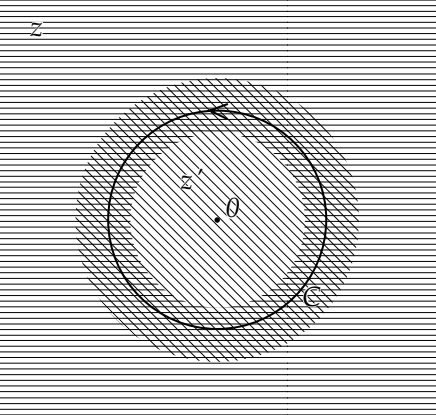
\includegraphics[width=0.5\textwidth]{figure/Fig5.3.jpg}\\
		\caption{Coordinate patches $z^{\prime}$ (diagonal hatching) and $z$ (horizontal hatching) with vertex operator at $z^{\prime}=0$. In the annular region, $z=z^{\prime}+z_{v}$.}\label{Fig5.3}
	\end{center}
\end{figure}

We keep the vertex operator at $z^{\prime}=0$ and encode its position into the transition function:
\begin{equation}
	z=z^{\prime}+z_{v}\label{5.4.16}
\end{equation}
The measure for $z_{v}, \bar{z}_{v}$ is given by \eqref{5.4.15}, where:
\begin{equation}
	\left.\frac{\partial z^{\prime}}{\partial z_{v}}\right|_{z}=-1\label{5.4.17}
\end{equation}
Therefore, the ghost insertion is:
\begin{equation}
	\int_{C} \frac{d z^{\prime}}{2 \pi i} b_{z^{\prime} z^{\prime}} \int_{C} \frac{d \bar{z}_{m}^{\prime}}{-2 \pi i} b_{\bar{z}^{\prime} \bar{z}^{\prime}}=b_{-1} \tilde{b}_{-1}\label{5.4.18}
\end{equation}
where $C$ is any contour surrounding the vertex operator as shown. Then, the complete expression for the $S$-matrix can be compactly written as:
\begin{equation}
	S(1 ; \ldots ; n)=\sum_{\text {compact topologies}} e^{-\lambda \chi} \int_{F} \frac{d^{m} t}{n_{R}}\left\langle\prod_{k=1}^{m} B_{k} \prod_{i=1}^{n} \hat{\mathscr{V}}_{i}\right\rangle\label{5.4.19}
\end{equation}
Here, $B_{k}$ is shorthand for the $b$ ghost insertion \eqref{5.4.15}, and $\hat{\mathscr{V}}$ represents $\tilde{c} c \mathscr{V}_{\mathrm{m}}$ for closed strings and $t_{a} c^{a} \mathscr{V}_{\mathrm{m}}$ for open strings. That is, we now treat all vertex operators as fixed and replace their coordinates with extra parameters in the transition functions. The number of moduli $m$ is:
\begin{equation}
	m=\mu+2 n_{\mathrm{c}}+n_{\mathrm{o}}-\kappa=-3 \chi+2 n_{\mathrm{c}}+n_{\mathrm{o}}
\end{equation}
where $n_{\mathrm{c}}$ and $n_{\mathrm{o}}$ are the numbers of closed string and open string vertex operators, respectively.

\eqref{5.4.19} shows that hatted vertex operators, i.e., those containing $\tilde{c} c$ or $t_{a} c^{a}$, are fundamental. This is exactly what the state-operator correspondence produces, and it is BRST-invariant. If the vertex operator is integrated, the ghost insertion \eqref{5.4.18} will remove $\tilde{c} c$ or $t_{a} c^{a}$. For example:
\begin{equation}
	b_{-1} \tilde{b}_{-1} \cdot \tilde{c} c \mathscr{V}_{\mathrm{m}}=\mathscr{V}_{\mathrm{m}}
\end{equation}
leaving the integrated form of the vertex operator. We wrote \eqref{5.4.19} from the Polyakov path integral, so vertex operators appear in the form of OCQ, but now we can use any BRST-invariant vertex operator.
	 \setcounter{section}{0}% Change chapter counter
 \numberwithin{equation}{section}% Equation counter belongs to section
 \numberwithin{figure}{section}% Figure counter belongs to section
 \setcounter{chapter}{5}

\chapter{\texorpdfstring{Tree-level amplitudes}{6 Tree-level amplitudes}} \label{cha:6}
We now study string interactions . In this chapter, we will investigate the lowest-order amplitudes, which originate from surfaces with positive Euler number . We first describe the relevant Riemann surfaces and calculate the required CFT expectation values . Next, we will study scattering amplitudes, first for open strings and then for closed strings . Along the way, we will introduce an important generalization in open string theory: Chan-Paton factors . At the end of this section, we will return to CFT and discuss the general properties of expectation values .

\section{Riemann surfaces} \label{sec:6.1}

There are three types of Riemann surfaces with positive Euler number: the sphere, the disk, and the projective plane .

\subsection*{The Sphere}

\begin{figure}[!htbp]
	\begin{center}
		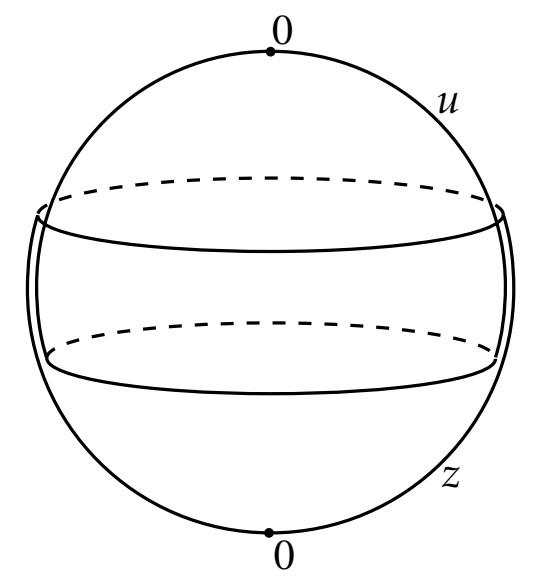
\includegraphics[width=0.5\textwidth]{figure/Fig6.1.jpg}\\
		\caption{A sphere constructed from the $z$ and $u$ coordinate charts .}\label{fig:6.1}
	\end{center}
\end{figure}

The sphere $S_2$ can be covered by two coordinate charts, as shown in figure \ref{fig:6.1} . We take disks $|z|<\rho$ and $|u|<\rho$, where $\rho>1$, and glue them via :
\begin{equation}
	u=1 / z  \label{6.1.1}
\end{equation}
\begin{tcolorbox}[breakable]
	\begin{proof}
		Consider \( x \in \mathbb{R}^n \), and define stereographic projection from the \textbf{north pole} of the unit sphere \( S^n \subset \mathbb{R}^{n+1} \) as:
		
		\[
		X^i = \frac{2x^i}{1 + |x|^2}, \quad
		X^{n+1} = \frac{|x|^2 - 1}{1 + |x|^2}
		\]
		where $x^i$ are coordinates on the plane and $X^i$ are the coordiantes on the sphere in embedding space. Now project this point on the sphere back to \( \mathbb{R}^n \) via stereographic projection from the \textbf{south pole}:
		
		\[
		x'^i = \frac{X^i}{1 + X^{n+1}}
		\]
		Substituting:
		
		\[
		x'^i = \frac{\frac{2x^i}{1 + |x|^2}}{1 + \frac{|x|^2 - 1}{1 + |x|^2}}
		= \frac{2x^i}{(1 + |x|^2) + (|x|^2 - 1)} = \frac{2x^i}{2|x|^2} = \frac{x^i}{|x|^2}
		\]
		Hence, the composition $(\mathbb{R}^n \xrightarrow{\text{north}} \mathbb{S}^n \xrightarrow{\text{south}} \mathbb{R}^n)$ gives:
		
		\[
		x^i \mapsto \frac{x^i}{|x|^2}
		\]
		which is the \textbf{inversion} in the unit sphere.
	\end{proof}
\end{tcolorbox}
In fact, we can take $\rho \to \infty$ . In this way, the coordinate $z$ is well-defined everywhere except at the "North Pole" $u=0$ . We can view the sphere as a Riemann surface by taking flat metrics on both coordinate charts and connecting them with a conformal (coordinate plus Weyl) transformation . Alternatively, we can view it as a Riemannian manifold with a globally defined metric . The general conformal gauge metric is :
\begin{equation}
	\dif s^{2}=\exp (2 \omega(z, \bar{z})) \dif z \dif \bar{z} \:. \label{6.1.2}
\end{equation}
Since $\dif z \dif \bar{z}=|z|^{4} \dif u \dif \bar{u}$, the condition for this metric to be non-singular at $u=0$ is that $\exp (2 \omega(z, \bar{z}))$ decays as $|z|^{-4}$ as $z \to \infty$ . For example :
\begin{equation}
	\dif s^{2}=\frac{4 r^{2}\, \dif z \dif \bar{z}}{(1+z \bar{z})^{2}}=\frac{4 r^{2}\, \dif u \dif \bar{u}}{(1+u \bar{u})^{2}} \label{6.1.3}
\end{equation}
describes a sphere with radius $r$ and curvature $R=2 / r^{2}$ .

According to the general discussion in section \ref{sec:5.2}, the sphere has no moduli but has 6 CKVs, making every metric ($\text{diff} \times \text{Weyl}$) equivalent to \eqref{6.1.3} . We observe this at the infinitesimal level . As in \eqref{5.2.8}, we look for holomorphic tensor fields $\delta g_{z z}(z)$ and holomorphic vector fields $\delta z(z)$ . These must be defined on the entire sphere, so we examine the transformation to the $u$ coordinate chart :
\begin{subequations}  \label{6.1.4}
	\begin{align}
		\delta u &=\frac{\partial u}{\partial z} \delta z=-z^{-2} \delta z \:, \label{6.1.4a} \\
		\delta g_{u u} &=\left(\frac{\partial u}{\partial z}\right)^{-2} \delta g_{z z}=z^{4} \delta g_{z z} \:. \label{6.1.4b} 
	\end{align}
\end{subequations}
Any holomorphic quadratic differential $\delta g_{z z}$ must be holomorphic with respect to $z$ and vanish as $z^{-4}$ at infinity; therefore, it must be identically zero . On the other hand, the CKV $\delta z$ being holomorphic at $u=0$ requires it to grow no faster than $z^{2}$ as $z \rightarrow \infty$ . Thus, the general CKV is :
\begin{subequations} \label{6.1.5}
	\begin{align}
		\delta z       &= a_{0}+a_{1} z+a_{2} z^{2}  \:, \label{6.1.5a} \\
		\delta \bar{z} &= a_{0}^{*}+a_{1}^{*} \bar{z}+a_{2}^{*} \bar{z}^{2} \:, \label{6.1.5b}
	\end{align}
\end{subequations}
which has 3 complex parameters or 6 real parameters, exactly as expected from the Riemann-Roch theorem . Exponentiating these infinitesimal transformations gives the \emph{Möbius group} :
\begin{equation}
	z^{\prime}=\frac{\alpha z+\beta}{\gamma z+\delta} \:. \label{6.1.6}
\end{equation}
Rescaling $\alpha, \beta, \gamma, \delta$ does not change the transformation, so we can fix $\alpha \delta-\beta \gamma=1$ and treat the set under global sign inversion of $\alpha, \beta, \gamma, \delta$ as equivalent, which defines the $PSL(2, \mathds{C})$ group . This is the most general coordinate transformation that is holomorphic on the entire $S_2$  . it is a one-to-one mapping including the point at infinity . Three of the six parameters correspond to ordinary rotations, forming the subgroup $SO(3)$ of $PSL(2, \mathds{C})$ .

\subsection*{The Disk}

The disk $D_2$ can be constructed from the sphere by identifying two points under reflection . For example, identify $z$ and $z^{\prime}$ such that :
\begin{equation}
	z^{\prime}=1 / \bar{z} \:. \label{6.1.7}
\end{equation}
In polar coordinates $z=r \me^{\mi \phi}$, this takes the reciprocal of the radius but preserves the angle, so the unit disk $|z| \leq 1$ is the fundamental domain after gluing . Points on the unit circle are fixed by the reflection, so it becomes a boundary . It is often more convenient to use the conformally equivalent inversion :
\begin{equation}
	z^{\prime}=\bar{z}  \label{6.1.8}
\end{equation}
Now the upper half-plane is the fundamental domain, and the real axis is the boundary .

The CKG of the disk is the subgroup of $PSL(2, \mathds{C})$ that keeps the boundary of the disk invariant . For the inversion \eqref{6.1.8}, this is the subgroup where $\alpha, \beta, \gamma, \delta$ in \eqref{6.1.6} are all real, namely $PSL(2, \mathds{R})$, the Möbius group of real parameters . One CKV is the ordinary rotational symmetry on the disk . Once again, all metrics are equivalent, and there are no moduli .

\subsection*{The Projective Plane}

The projective plane $RP_2$ can also be obtained as a $\mathds{Z}_{2}$ identification of the sphere . Glue points $z$ and $z^{\prime}$ such that :
\begin{equation}
	z^{\prime}=-1 / \bar{z} \label{6.1.9}
\end{equation}
These points are antipodal points in the round metric \eqref{6.1.3} . There are no fixed points, so there is no boundary in the resulting space, but the space is non-orientable . A fundamental domain for this gluing is the unit disk $|z| \leq 1$, but points $\me^{\mi \phi}$ and $-\me^{\mi \phi}$ are identified . Another choice is the upper $z$-plane, where there are no moduli . The CKG is the subgroup of $PSL(2, \mathds{C})$ reflecting the \eqref{6.1.9} identification; this is the ordinary rotation group $SO(3)$ . Both the disk and the projective plane can be represented as spheres with points identified under a $\mathds{Z}_{2}$ transformation or \emph{involution} . In fact, every worldsheet can be obtained from a closed oriented surface by identification under one or two $\mathds{Z}_{2}$ involutions . Thus, Green's functions can be obtained using the method of images .

\section{Expectation values of scalars} \label{sec:6.2}

The basic quantities we need are the expectation values of vertex operators . To develop several useful techniques and viewpoints, we will calculate them in three different ways: direct path integrals, using holomorphy, and the operator method later in this chapter .

The path integral method has already been used for the Faddeev-Popov determinant in section \ref{sec:5.3} and for the harmonic oscillator in the appendix . Starting from a general functional :
\begin{equation}
	Z[J]=\left\langle\exp \left(\mi \int \dif^{2} \sigma\: J(\sigma) \cdot X(\sigma)\right)\right\rangle \label{6.2.1}
\end{equation}
where $J_{\mu}(\sigma)$ is arbitrary . From now on, we work on an arbitrary compact two-dimensional surface $M$, and the spacetime dimension is $d$ . We expand $X^{\mu}(\sigma)$ on a complete basis $\mathsf{X}_{I}(\sigma)$ :
\begin{subequations} \label{6.2.2}
	\begin{align}
		X^{\mu}(\sigma) &= \sum_{I} x_{I}^{\mu} \mathsf{X}_{I}(\sigma) \:, \label{6.2.2a} \\
		\nabla^{2} \mathsf{X}_{I} &= -\omega_{I}^{2} \mathsf{X}_{I} \:,  \label{6.2.2b} \\
		\int_{M} \dif^{2} \sigma\: g^{1 / 2} \mathsf{X}_{I} \mathsf{X}_{I^{\prime}} &= \delta_{I I^{\prime}} \:. \label{6.2.2c} 
	\end{align}	
\end{subequations}
Then :
\begin{equation}
	Z[J]=\prod_{I, \mu} \int \dif x_{I}^{\mu} \exp \left(-\frac{\omega_{I}^{2} x_{I}^{\mu} x_{I \mu}}{4 \pi \alpha^{\prime}}+\mi x_{I}^{\mu} J_{I \mu}\right) \:, \label{6.2.3}
\end{equation}
where :
\begin{equation}
	J_{I}^{\mu}=\int \dif^{2} \sigma J^{\mu}(\sigma) \mathsf{X}_{I}(\sigma) \:. \label{6.2.4}
\end{equation}
Except for the constant mode :
\begin{equation}
	\mathsf{X}_{0}=\left(\int \dif^{2} \sigma \: g^{1 / 2}\right)^{-1 / 2} \:, \label{6.2.5}
\end{equation}
this integral is Gaussian . The action for the constant mode is zero, so it yields a $\delta$-function .

\begin{tcolorbox}
	\begin{remark}
		For $I=0$, \eqref{6.2.3} gives :
		\[
		\int \dif x^{\mu}_{0} \: \exp (\mi x^{\mu}_{0}J_{0\mu}) \propto \delta^{d}(J_{0}) \:.
		\]
	\end{remark}
\end{tcolorbox}
\noindent Evaluating the integral yields :
\begin{align}
	Z[J] &= \mi(2 \pi)^{d} \delta^{d}(J_{0}) \prod_{I \neq 0} \left(\frac{4 \pi^{2} \alpha^{\prime}}{\omega_{I}^{2}}\right)^{d / 2} \exp \left(-\frac{\pi \alpha^{\prime} J_{I} \cdot J_{I}}{\omega_{I}^{2}}\right) \nonumber  \\
	&= \mi(2 \pi)^{d} \delta^{d}\left(J_{0}\right)\left(\operatorname{det}^{\prime} \frac{-\nabla^{2}}{4 \pi^{2} \alpha^{\prime}}\right)^{-d / 2} \nonumber  \\
	& \qquad \quad \times \exp \left(-\frac{1}{2} \int \dif^{2} \sigma \, \dif^{2} \sigma^{\prime}\: J(\sigma) \cdot J(\sigma^{\prime}) 
	G^{\prime}(\sigma, \sigma^{\prime})\right) \:. \label{6.2.6}
\end{align}
As discussed in sections \ref{sec:2.1} and \ref{sec:3.2}, the Gaussian integral generated by the timelike mode $x_{I}^{0}$ has the wrong sign, so it is defined via contour rotation $x_{I}^{0} \to-\mi x_{I}^{d}, I \neq 0$ . The primed Green's function removes the zero-mode contribution :
\begin{equation}
	G^{\prime}(\sigma_{1}, \sigma_{2})=\sum_{I \neq 0} \frac{2 \pi \alpha^{\prime}}{\omega_{I}^{2}} \mathsf{X}_{I}(\sigma_{1}) \mathsf{X}_{I}(\sigma_{2}) \:. \label{6.2.7}
\end{equation}
It satisfies the differential equation :
\begin{align}
	-\frac{1}{2 \pi \alpha^{\prime}} \nabla^{2} G^{\prime}(\sigma_{1}, \sigma_{2}) 
	&=\sum_{I \neq 0} \mathsf{X}_{I}(\sigma_{1}) \mathsf{X}_{I}(\sigma_{2})  \nonumber \\
	&=g^{-1 / 2} \delta^{2}(\sigma_{1}-\sigma_{2})-\mathsf{X}_{0}^{2}  \:, \label{6.2.8}
\end{align}
where the completeness of $\mathsf{X}_{I}$ is used . An ordinary Green's function with a $\delta$-function source does not exist . It would correspond to the electrostatic potential of a single charge, but on a compact surface, field lines flowing out of the source have nowhere to go . The $\mathsf{X}_{0}^{2}$ term can be viewed as a background charge distribution used to neutralize the system .

\subsection*{The Sphere}
Specifically on the sphere, the solution to the differential equation \eqref{6.2.8} is :
\begin{equation}
	G^{\prime}(\sigma_{1}, \sigma_{2})=-\frac{\alpha^{\prime}}{2} \ln |z_{12}|^{2}+f(z_{1}, \bar{z}_{1})+f(z_{2}, \bar{z}_{2}) \:. \label{6.2.9}
\end{equation}
\begin{tcolorbox}
	\begin{remark}
		On the sphere $g=\me^{4 \omega}$, $\nabla^{2}=\me^{-2 \omega} \partial \bar{\partial}$, so \eqref{6.2.8} becomes :
		\[
		\partial \bar{\partial} G^{\prime}=-2 \pi \alpha^{\prime} \delta^{2}(\sigma_{1}-\sigma_{2})
		+2 \pi \alpha^{\prime} \me^{2 \omega}\,\mathsf{X}_{0}^{2} 
		\]
		where $\partial \bar{\partial} \ln |z_{12}|^{2}=2 \pi \delta^{2}(z, \bar{z})=4 \pi \delta^{2}(\sigma_{1}-\sigma_{2})$ .
	\end{remark}
\end{tcolorbox}
\noindent where :
\begin{equation}
	f(z, \bar{z})=\frac{\alpha^{\prime} \mathsf{X}_{0}^{2}}{4} 
	\int \dif^{2} z^{\prime}\: \exp [2 \omega(z^{\prime}, \bar{z}^{\prime})] \ln|z-z^{\prime}|^{2}+k \:. \label{6.2.10}
\end{equation}
The condition that $G^{\prime}$ is orthogonal to $\mathsf{X}_{0}$ determines the constant $k$, but in any case, we will see that all expectation values is independent of the function $f$. It originates from the background charge, but the $\delta$-function from the zero-mode integration forces overall neutrality, $J_{0}^{\mu}=0$, so the background field has no net contribution .

Now consider the path integral containing a product of tachyon vertex operators :
\begin{equation}
	A_{S_{2}}^{n}(k, \sigma)=\left\langle\left[\me^{\mi k_{1} \cdot X(\sigma_{1})}\right]_{\mathrm{r}}
	\left[\me^{\mi k_{2} \cdot X(\sigma_{2})}\right]_{\mathrm{r}} \cdots
	\left[\me^{\mi k_{n} \cdot X(\sigma_{n})}\right]_{\mathrm{r}}\right\rangle_{S_{2}} \:. \label{6.2.11}
\end{equation}
This corresponds to :
\begin{equation}
	J(\sigma)=\sum_{i=1}^{n} k_{i} \delta^{2}(\sigma-\sigma_{i}) \:. \label{6.2.12}
\end{equation}
Then the amplitude \eqref{6.2.6} becomes :
\begin{align}
	A_{S_{2}}^{n}(k, \sigma) &=\mi C_{S_{2}}^{X}(2 \pi)^{d} \delta^{d}({\textstyle \sum_{i}} k_{i}) \nonumber \\
	& \quad \times \exp \Biggl(-\sum_{ i<j}^{n} k_{i} \cdot k_{j} G^{\prime}(\sigma_{i}, \sigma_{j})
	-\frac{1}{2} \sum_{i=1}^{n} k_{i}^{2} G_{\mathrm{r}}^{\prime}(\sigma_{i}, \sigma_{i})\Biggr) \:. \label{6.2.13}
\end{align}
The constant here is :
\begin{equation}
	C_{S_{2}}^{X}=\mathsf{X}_{0}^{-d}\left(\operatorname{det}^{\prime} \frac{-\nabla^{2}}{4 \pi^{2} \alpha^{\prime}}\right)_{S_{2}}^{-d/2} 
	\:. \label{6.2.14}
\end{equation}
\begin{tcolorbox}
	\begin{remark}
		According to \eqref{6.2.4} and \eqref{6.2.5}, $J_{0}=\int \dif^{2} \sigma \: \mathsf{X}_{0} J(\sigma)= \mathsf{X}_{0} \sum_{i} k_{i}$, so $\delta^{d}(J_{0})=\mathsf{X}_{0}^{-d} \delta^{d}(\sum_{i} k_{i})$ .
	\end{remark}
\end{tcolorbox}
\noindent The determinant can be regularized and calculated, but we do not need to calculate it explicitly . We adopt the renormalization from section \ref{sec:3.6} such that self-contractions include :
\begin{equation}
	G_{\mathrm{r}}^{\prime}(\sigma, \sigma^{\prime})=G^{\prime}(\sigma, \sigma^{\prime})
	+\frac{\alpha^{\prime}}{2} \ln d^{2}(\sigma, \sigma^{\prime}) \:. \label{6.2.15}
\end{equation}
Note that :
\begin{equation}
	G_{\mathrm{r}}^{\prime}(\sigma, \sigma)=2 f(z, \bar{z})+\alpha^{\prime} \omega(z, \bar{z}) \label{6.2.16}
\end{equation}
is finite . Then the path integral on the sphere is :
\begin{equation}
	A_{S_{2}}^{n}(k, \sigma)=\mi C_{S_{2}}^{X}(2 \pi)^{d} \delta^{d}({\textstyle \sum_{i}} k_{i}) 
	\exp \left(-\frac{\alpha^{\prime}}{2} \sum_{i} k_{i}^{2} \omega\left(\sigma_{i}\right)\right) 
	\prod_{i<j}|z_{i j}|^{\alpha^{\prime} k_{i} \cdot k_{j}} \:. \label{6.2.17}
\end{equation}
The dependence on the conformal factor $\omega(\sigma)$ is obtained from the Weyl anomaly of the vertex operators . For on-shell operators, it will cancel the variation of $g^{1/2}$ . We will take the metric to be flat (pushing the curvature to infinity) in a large region containing all vertex operators; thus, terms in $\omega(\sigma_{i})$ are dropped .
\begin{tcolorbox}[breakable]
	Notes on \eqref{6.2.16}:
	\[
	\ln d^{2}(\sigma, \sigma^{\prime})-\ln |z_{12}|^{2}=
	\ln \left(\frac{\int \me^{2 \omega} \: \dif z \dif \bar{z}}{\int \dif z \dif  \bar{z}}\right)=2 \omega	
	\]
	Notes on \eqref{6.2.17}: Taking $n=2$ as an example, the part depending on $f$ is 
	\[
	k_{1} k_{2} (f_{1}+f_{2})+\frac{1}{2} k_{1}^{2} \cdot 2 f_{1}+\frac{1}{2} k_{2}^{2} \cdot 2 f_{2} 
	=(k_{1} f_{1}+k_{2} f_{2})(k_{1}+k_{2})
	\]
	Since the path integral contains $\delta(\sum_{i} k_{i})= k_{1}+k_{2}$, it is independent of $f$ .
\end{tcolorbox}

Higher-order vertex operators are exponentials multiplied by partial derivatives of $X^{\mu}$, so we further need :
\begin{equation}
	\Biggl\langle\prod_{i=1}^{n}\left[\me^{\mi k_{i} \cdot X(z_{i}, \bar{z}_{i})}\right]_{\mathrm{r}} 
	\prod_{j=1}^{p} \partial X^{\mu_{j}}(z_{j}^{\prime}) \prod_{k=1}^{q} \bar{\partial} X^{\nu_{k}}(\bar{z}_{k}^{\prime \prime})\Biggr\rangle \biggr._{\!\!S_{2}} \:. \label{6.2.18}
\end{equation}
This is given by summing over all contractions, where each $\partial X$ or $\bar{\partial} X$ must contract with an exponential or other $\partial X$ and $\bar{\partial} X$ . The $XX$ contraction is $-\frac{1}{2} \alpha^{\prime} \ln |z|^{2}$, and $f$ is again dropped in the final expression . This result is summarized as :
\begin{align}
	&\mi C_{S_{2}}^{X}(2 \pi)  \delta^{d}({\textstyle\sum_{i} }k_{i}) 
	\exp\Biggl(-\frac{\alpha'}{2}\sum_{i}k_{i}^{2}\omega(\sigma_{i})\Biggr)
	\prod_{i<j}^{n}|z_{i j}|^{\alpha^{\prime} k_{i} \cdot k_{j}}  \nonumber \\
	& \qquad \quad \times\Biggl\langle 
	\prod_{j=1}^{p}\Bigl[v^{\mu_{j}}(z_{j}^{\prime})+q^{\mu_{j}}(z_{j}^{\prime})\Bigr] 
	\prod_{k=1}^{q}\Bigl[\tilde{v}^{\nu_{k}}(\bar{z}_{k}^{\prime \prime})+\tilde{q}^{\nu_{k}}(\bar{z}_{k}^{\prime \prime})\Bigr]\Biggr\rangle  \label{6.2.19}
\end{align}
where :
\begin{equation}
	v^{\mu}(z)=- \mi \frac{\alpha^{\prime}}{2} \sum_{i=1}^{n} \frac{k_{i}^{\mu}}{z-z_{i}}, \qquad 
	\tilde{v}^{\mu}(\bar{z})=-\mi \frac{\alpha^{\prime}}{2} \sum_{i=1}^{n} \frac{k_{i}^{\mu}}{\bar{z}-\bar{z}_{i}} \label{6.2.20}
\end{equation}
originate from contractions with the exponentials . The expectation value of $q^{\mu}=\partial X^{\mu}-v^{\mu}$ is given by contraction with $-\eta^{\mu \nu}(z-z^{\prime})^{-2} \alpha^{\prime} / 2$ and summing, while the expectation value of $\tilde{q}^{\nu}$ is given by conjugation .
\begin{tcolorbox}[breakable]
	\begin{proof}
The operator product can be expanded as following:
\begin{align}
	\prod_{i=1}^{n}\normal{&\bigl[\me^{\mi k_i\cdot X(z_i,\bar z_i)}\bigr]_{\mathrm r}}
	\prod_{j=1}^{p}\normal{\partial X^{\mu_j}(z'_j)}
	\prod_{k=1}^{q}\normal{\bar\partial X^{\nu_k}(\bar z''_k)}
	\nonumber\\[4pt]
	&=\sum_{i=1}^{n}
	\contraction{}{\partial X^{\mu_1}(z'_1)}{\,}{e^{\mi k_i\cdot X(z_i,\bar z_i)}}
	\partial X^{\mu_1}(z'_1)e^{\mi k_i\cdot X(z_i,\bar z_i)}
	\normal{
		\prod_{\substack{l=1\\ l\neq i}}^{n}\bigl[\me^{\mi k_l\cdot X(z_l,\bar z_l)}\bigr]_{\mathrm r}
		\prod_{j=2}^{p}\partial X^{\mu_j}(z'_j)
		\prod_{k=1}^{q}\bar\partial X^{\nu_k}(\bar z''_k)}
	\nonumber\\
	&\qquad+\sum_{j=2}^{p}
	\wick{\partial \c1 X^{\mu_1}(z'_1)\partial \c1 X^{\mu_j}(z'_j)}
	\normal{
		\prod_{i=1}^{n}\bigl[\me^{\mi k_i\cdot X(z_i,\bar z_i)}\bigr]_{\mathrm r}
		\prod_{\substack{l=2\\ l\neq j}}^{p}\partial X^{\mu_l}(z'_l)
		\prod_{k=1}^{q}\bar\partial X^{\nu_k}(\bar z''_k)}
	\nonumber\\
	&\qquad+\sum_{k=1}^{q}
	\wick{\partial \c1 X^{\mu_1}(z'_1)\bar\partial \c1 X^{\nu_k}(\bar z''_k)}
	\normal{
		\prod_{i=1}^{n}\bigl[\me^{\mi k_i\cdot X(z_i,\bar z_i)}\bigr]_{\mathrm r}
		\prod_{j=2}^{p}\partial X^{\mu_j}(z'_j)
		\prod_{\substack{l=1\\ l\neq k}}^{q}\bar\partial X^{\nu_l}(\bar z''_l)}
	\nonumber\\[6pt]
	&\qquad+\sum_{i=1}^{n}
	\contraction{}{\bar\partial X^{\nu_1}(\bar z''_1)}{\,}{e^{\mi k_i\cdot X(z_i,\bar z_i)}}
	\bar\partial X^{\nu_1}(\bar z''_1)e^{\mi k_i\cdot X(z_i,\bar z_i)}
	\normal{
		\prod_{\substack{l=1\\ l\neq i}}^{n}\bigl[\me^{\mi k_l\cdot X(z_l,\bar z_l)}\bigr]_{\mathrm r}
		\prod_{j=1}^{p}\partial X^{\mu_j}(z'_j)
		\prod_{k=2}^{q}\bar\partial X^{\nu_k}(\bar z''_k)}
	\nonumber\\
	&\qquad+\sum_{k=2}^{q}
	\wick{\bar\partial \c1 X^{\nu_1}(\bar z''_1)\bar\partial \c1 X^{\nu_k}(\bar z''_k)}
	\normal{
		\prod_{i=1}^{n}\bigl[\me^{\mi k_i\cdot X(z_i,\bar z_i)}\bigr]_{\mathrm r}
		\prod_{j=1}^{p}\partial X^{\mu_j}(z'_j)
		\prod_{\substack{l=2\\ l\neq k}}^{q}\bar\partial X^{\nu_l}(\bar z''_l)}
	\nonumber\\
	&\qquad+\sum_{j=1}^{p}
	\wick{\bar\partial \c1 X^{\nu_1}(\bar z''_1)\partial \c1 X^{\mu_j}(z'_j)}
	\normal{
		\prod_{i=1}^{n}\bigl[\me^{\mi k_i\cdot X(z_i,\bar z_i)}\bigr]_{\mathrm r}
		\prod_{\substack{l=1\\ l\neq j}}^{p}\partial X^{\mu_l}(z'_l)
		\prod_{k=2}^{q}\bar\partial X^{\nu_k}(\bar z''_k)}.
\end{align}
Each holomorphic $\del X^\mu(z')$ (or anti holomorphic term $\bar\del X^\mu(z')$) upon contraction with the vertex operator generates the classical function $v^\mu$ times the vertex operator itself:
		\begin{align}
			\sum_{i=1}^n \contraction{}{X^\mu(z')}{\,}{e^{i k_i \cdot X(z_i)}}
			 \partial X^\mu(z') e^{i k_i \cdot X(z_i)}		
			&= \sum_{i=1}^n \left( i k_i^\rho \expval{\del X^\mu(z') X_\rho(z_i)} \right) \normal{\prod e^{ik \cdot X}} \nonumber \\
			&= \underbrace{\sum_{i=1}^n \left( - \frac{i \alpha'}{2} \frac{k_i^\mu}{z' - z_i} \right)}_{v^\mu(z')} \normal{\prod e^{ik \cdot X}}
		\end{align}
		Since the vertex operator are left over one can further contract it with the remaining operators in the same term. Each contraction appears as a factor of $v^{\mu}$ or $\bar v^{\mu}$. Contraction of vertex operator in those terms produce $\normal{\ldots}$ which annihilate the vacuum due to absence of commuting zero mode and hence drop out. To evaluate the contraction between $\partial X$, we need
		\begin{equation}
			\wick{ \c1 {\del X^\mu(z_1')} \c1 {\del X^\nu(z_2')} } 
			= \expval{q^\mu(z_1') q^\nu(z_2')} 
			= -\frac{\alpha'}{2} \frac{\eta^{\mu\nu}}{(z_1' - z_2')^2}
		\end{equation}
		and the last expression to evaluate the contraction between vertex operator is:
		\begin{equation}
			\wick{ \c1 {\normal{e^{i k_i \cdot X(z_i)}}} \c1 {\normal{e^{i k_j \cdot X(z_j)}}} } 
			= \exp\left( -k_i \cdot k_j \expval{X(z_i) X(z_j)} \right)
			= |z_i - z_j|^{\alpha' k_i \cdot k_j}
		\end{equation}
		To implement this efficiently, we will follow the following decomposition to isolate the contraction with $e^{ik\cdot  X}$ to write the result cleanly. 
		\begin{equation}
			\del X^\mu(z') \to v^\mu(z') + q^\mu(z')
		\end{equation}
		where $v^\mu(z')$ originates from contraction with $e^{ik\cdot  X}$ and $q^\mu(z')$ only contracts with other $q^\mu(z')$. Combining all factors, including the normalization $C_{S_2}^X$ and the regularization term $\omega(z)$, the amplitude is:
		
		\begin{align}
			A_{S_{2}} &= \mathcal{C}_{S_{2}}^{X}(2 \pi)  \delta^{d}\left(\sum k_{i}\right) 
			\exp\left(-\frac{\alpha'}{2}\sum_{i}k_{i}^{2}\omega(z_{i})\right)
			\prod_{i<j}^{n}|z_{i j}|^{\alpha^{\prime} k_{i} \cdot k_{j}} \nonumber \\
			&\quad \times \expval{ 
				\prod_{j=1}^{p} \left[ v^{\mu_{j}}(z_{j}^{\prime}) + q^{\mu_{j}}(z_{j}^{\prime}) \right] 
				\prod_{k=1}^{q} \left[ \tilde{v}^{\nu_{k}}(\bar{z}_{k}^{\prime \prime}) + \tilde{q}^{\nu_{k}}(\bar{z}_{k}^{\prime \prime}) \right] 
			}
		\end{align}
		QED.
	\end{proof}
\end{tcolorbox}
Now we re-calculate in a different way, using holomorphy . As an example, consider :
\begin{equation}
	\langle\partial X^{\mu}(z_{1}) \partial X^{\nu}(z_{2})\rangle_{S_{2}} \:. \label{6.2.21}
\end{equation}
The OPE determines it to be :
\begin{equation}
	-\frac{\alpha^{\prime} \eta^{\mu \nu}}{2 z_{12}^{2}}\langle 1\rangle_{S_{2}}+g(z_{1}, z_{2}) \:, \label{6.2.22}
\end{equation}
where $g(z_{1}, z_{2})$ is holomorphic in both variables . In the $u$ coordinate chart :
\begin{equation}
	\partial_{u} X^{\mu}=-z^{2} \partial_{z} X^{\mu} \:, \label{6.2.23}
\end{equation}
so the condition for holomorphy at $u=0$ is that the expectation value of $\partial_{z} X^{\mu}$ decays as $z^{-2}$ as $z$ goes to infinity . More generally, the behavior of a tensor with weight $(h, 0)$ at infinity is $z^{-2 h}$ . Focusing on the correlation of \eqref{6.2.22} with respect to $z_{1}$ at fixed $z_{2}$, this implies $g(z_{1}, z_{2})$ decays as $z_{1}^{-2}$ at infinity, hence the holomorphic factor is zero . Compared with the path integral result \eqref{6.2.19}, this is consistent . Although $\langle 1\rangle_{S_{2}}$ seems to diverge like $\delta(0)$, this is just the zero-mode divergence from the infinite spacetime volume . Regarding the expectation value of a product of vertex operators :
\begin{equation}
	A_{S_{2}}^{n}(k, \sigma)=\left\langle\prod_{i=1}^{n}:\mathrel{\me^{\mi k_{i} \cdot X(z_{i}, \bar{z}_{i})}}:\right\rangle \Big._{\!S_{2}}
	\label{6.2.24}
\end{equation}
calculating with this method is less direct because they are not holomorphic . In fact, they factorize into holomorphic and anti-holomorphic parts, but this is subtle and is best introduced in the language of operators, which we will do in chapter \ref{cha:8} . We use the holomorphy of the translation current . Consider the expectation value with an additional current $\partial X^{\mu}(z)$ . The OPE of the current and vertex operators determines the singularity at $z$ :
\begin{equation}
	\left\langle\partial X^{\mu}(z) \prod_{i=1}^{n}:\mathrel{\me^{\mi k_{i} \cdot X(z_{i}, \bar{z}_{i})}}:\right
	\rangle\bigg._{\!S_{2}}=-\frac{\mi \alpha^{\prime}}{2} A_{S_{2}}^{n}(k, \sigma) \sum_{i=1}^{n} \frac{k_{i}^{\mu}}{z-z_{i}} 
	+\text{terms holomorphic at } z \:. \label{6.2.25}
\end{equation}
\begin{tcolorbox}
	\begin{proof}
		Use
		\begin{equation}
		\sum_{i=1}^{n}\contraction{}{X^\mu(z')}{\,}{e^{i k_i \cdot X(z_i)}}\partial X^\mu(z') e^{i k_i \cdot X(z_i)}	= \left( - \frac{i \alpha'}{2} \frac{k_i^\mu}{z' - z_i} \right) \normal{\prod_{i=1}^{n} e^{ik \cdot X}}
		\end{equation}
	\end{proof}
\end{tcolorbox}
Now observe $z \rightarrow \infty$ . The condition that $\partial_{u} X^{\mu}$ is holomorphic at $u=0$ again requires this expectation value to vanish as $z^{-2}$ as $z \rightarrow \infty$ . Then the holomorphic terms in \eqref{6.2.25} are zero, and the term at order $z^{-1}$ is zero . We find momentum conservation :
\begin{equation}
	A_{S_{2}}^{n}(k, \sigma) \sum_{i=1}^{n} k_{i}^{\mu}=0 \:. \label{6.2.26}
\end{equation}
We state this in a slightly different way . Consider the contour integral of the spacetime translation current :
\begin{equation}
	p^{\mu}=\frac{1}{2 \pi \mi} \oint_{C}(\dif z \: j_{z}^{\mu}-\dif \bar{z}\: j_{\bar{z}}^{\mu}) \:, \label{6.2.27}
\end{equation}
where the contour $C$ encloses all exponential operators . There are two ways to calculate it . One is to shrink the contour $C$ until it becomes a small circle around each vertex operator, which picks out the $(z-z_{i})^{-1}$ term from each OPE and gives $\sum_{i=1}^{n} k_{i}^{\mu}$ . The other is to expand it until it is a small circle on the $u$ coordinate chart: due to holomorphy at $u=0$, it must be zero . This discussion of deforming contours is widely used in CFT . We have used the OPE to determine singularities and then used holomorphy to completely determine the dependence on $z$ . Now let us look at the second term of the OPE as $z \rightarrow z_{1}$ . Expanding \eqref{6.2.25} gives :
\begin{equation}
	-\frac{\mi \alpha^{\prime}}{2} A_{S_{2}}^{n}(k, \sigma)\left(\frac{k_{1}^{\mu}}{z-z_{1}}+\sum_{i=2}^{n} \frac{k_{i}^{\mu}}{z_{1}-z_{i}}+O(z-z_{1})\right) \:. \label{6.2.28}
\end{equation}
\begin{tcolorbox}[breakable]
	\begin{proof}
		Use 
		\begin{align}
			\frac{1}{z-z_i} &=\frac{1}{z_1-z_i}\frac{z_1-z_i}{z-z_i}=\frac{1}{z_1-z_i}\frac{1}{1+\frac{z-z_1}{z_1-z_i}}=\frac{1}{z_1-z_i}+O(z-z_1)
		\end{align}
		in \eqref{6.2.25}
	\end{proof}
\end{tcolorbox}
Contracting with $\mi k_{1}^{\mu}$, the $(z-z_{1})^{0}$ order term must be consistent with the OPE :
\begin{align}
	\mi k_{1} \cdot \partial X(z): \mathrel{\me^{\mi k_{1} \cdot X(z_{1}, \bar{z}_{1})}}: =\frac{\alpha^{\prime} k_{1}^{2}}{2(z-z_{1})} :\mathrel{\me^{\mi k_{1} \cdot X(z_{1}, \bar{z}_{1})}}:
	+ \: \partial_{z_{1}}{:\mathrel{\me^{\mi k_{1} \cdot X(z_{1}, \bar{z}_{1})}}:}+ O(z-z_{1}) \:. \label{6.2.29}
\end{align}
This implies :
\begin{equation}
	\partial_{z_{1}} A_{S_{2}}^{n}(k, \sigma)=\frac{\alpha^{\prime}}{2} A_{S_{2}}^{n}(k, \sigma) \sum_{i=2}^{n} \frac{k_{1} \cdot k_{i}}{z_{1 i}} \:. \label{6.2.30}
\end{equation}
Integrating and using conjugate equations as well as momentum conservation . In the sense of normalization difference, this determines the path integral :
\begin{equation}
	A_{S_{2}}^{n}(k, \sigma) \propto \delta^{d}({\textstyle \sum_{i} k_{i}}) 
	\prod_{i<j}^{n} |z_{i j}|^{\alpha^{\prime} k_{i} \cdot k_{j}} \:, \label{6.2.31}
\end{equation}
which is consistent with the first method . Note that for comparison, we must push the curvature to infinity ($\omega(\sigma_{i})=0$), which makes $[]_{\mathrm{r}}=::$ .
\begin{tcolorbox}
	\begin{remark}
		Note that \eqref{6.2.31} does satisfy \eqref{6.2.30} with
		\begin{equation}
			\partial_z [z_{1i}^{\frac{\alpha' k_1\cdot k_i}{2}}] = \frac{\alpha'k_1\cdot k_i}{2} \frac{z_{1i}}{z_1-z_i}
		\end{equation}
	\end{remark}
\end{tcolorbox}
It is worth noting that the intermediate steps of the path method depend on the specific choice of the Riemann metric . This metric is needed to preserve coordinate invariance in these steps . Two different metrics, if Weyl equivalent, still give different Laplacians and eigenfunctions . But in the end, in string theory, these correlations must be dropped . The second method uses only the fundamental properties of the Riemann surface, its holomorphy .

\subsection*{The Disk}
The extension to the disk is direct . By taking the representation of the sphere above and constraining $z$ to the upper complex plane, we obtain the representation of the disk . The Neumann boundary term is interpreted as an image charge :
\begin{equation}
	G^{\prime}(\sigma_{1}, \sigma_{2})=-\frac{\alpha^{\prime}}{2} \ln |z_{1}-z_{2}|^{2}
	-\frac{\alpha^{\prime}}{2} \ln |z_{1}-\bar{z}_{2}|^{2} \:, \label{6.2.32}
\end{equation}
differing by a term that is dropped due to momentum conservation . Then :
\begin{align}
	\left\langle\prod_{i=1}^{n}: \mathrel{\me^{\mi k_{i} \cdot X(z_{i}, \bar{z}_{i})}}:\right\rangle \bigg._{\!\!D_{2}} 
	=& \mi C_{D_{2}}^{X} (2 \pi)^{d} \delta^{d}({\textstyle\sum_{i} k_{i}}) 
	\prod_{i=1}^{n}|z_{i}-\bar{z}_{i}|^{\alpha^{\prime} k_{i}^{2} / 2}  \nonumber \\
	& \times \prod_{ i<j}^{n} |z_{i}-z_{j}|^{\alpha^{\prime} k_{i} \cdot k_{j} }
	|z_{i}-\bar{z}_{j}|^{\alpha^{\prime} k_{i} \cdot k_{j}} \:. \label{6.2.33}
\end{align}
For expectation values containing $\partial_{a} X^{\mu}$, one again sums over contractions, but now using the Green's function \eqref{6.2.32} . Note that $\partial X^{\mu}(z) \bar{\partial} X^{\nu}(\bar{z}^{\prime})$ (or $q^{\mu}(z) \tilde{q}^{\nu}(\bar{z}^{\prime})$) has a non-zero contraction .

For two points on the boundary, the two terms in the Green's function \eqref{6.2.32} are equal; even after subtracting the first term in normal ordering, the Green's function still diverges at zero interval . For this reason, boundary operators must be defined using boundary normal ordering, where the subtraction is doubled :
\begin{equation}
	\bno X^{\mu}(y_{1}) X^{\nu}(y_{2})\bno = X^{\mu}(y_{1}) X^{\nu}(y_{2})+2 \alpha^{\prime} \eta^{\mu \nu} 
	\ln |y_{1}-y_{2}| \:,  \label{6.2.34}
\end{equation}
where $y$ represents coordinates on the real axis . Combinatorics is the same as for other forms of normal ordering . The expectation values of boundary normal ordered boundary operators have the same well-behaved properties (no singularities) as internal conformal normal ordered operators .
\begin{tcolorbox}[breakable]
	\begin{remark}
A more intuitive way to see why the standard normal ordering fails on the disk boundary is to use the \textbf{method of images}. On the disk \(D_2\), the Green's function for a free boson with Neumann (or Dirichlet) boundary conditions can be written as a sum of a direct term and an image term:

\begin{equation}
	\langle X(z_1) X(z_2) \rangle \sim -\frac{\alpha'}{2} \ln |z_1 - z_2|^2 \;-\; \frac{\alpha'}{2} \ln |z_1 - \bar{z}_2|^2 + \text{finite}.\label{prop}
\end{equation}

The first term is the usual bulk propagator; the second term comes from the image charge at \(\bar{z}_2\) needed to satisfy the boundary condition (e.g., Neumann on the real axis). 

On the boundary, we have \(z = \bar{z}\). Therefore, when both points are on the boundary, \(z_1\) and \(z_2\) are real, and
\begin{equation}
	|z_1 - \bar{z}_2|^2 = |z_1 - z_2|^2.
\end{equation}

Thus the propagator \eqref{prop} restricted to the boundary becomes
\begin{equation}
	\langle X(z_1) X(z_2) \rangle \big|_{\partial} \sim -\alpha' \ln |z_1 - z_2|^2 + \text{finite}.
\end{equation}

The standard normal ordering subtracts only \(\frac{\alpha'}{2} \ln |z_1 - z_2|^2\), which is \emph{half} of the actual singularity. Consequently, the normal‑ordered product retains a residual divergence:

\begin{equation}
	\langle :X(z_1)X(z_2): \rangle \big|_{\partial} \sim -\frac{\alpha'}{2} \ln |z_1 - z_2|^2 + \text{finite}.
\end{equation}

The boundary normal ordering \(\bno \cdots \bno\) is defined to subtract the \emph{full} boundary singularity:

\begin{equation}
	\bno X(y_1) X(y_2) \bno = X(y_1) X(y_2) + 2\alpha' \ln(y_1 - y_2).
\end{equation}
which renders the correlators finite on the boundary.
\end{remark}
\end{tcolorbox}
If an expectation value contains both boundary exponentials and internal exponentials, each with appropriate normal ordering, drop the $|z_{i}-\bar{z}_{i}|^{\alpha^{\prime} k_{i}^{2} / 2}$ factor for the boundary operators and take the appropriate limit of the internal result \eqref{6.2.33} . Explicitly, for exponentials all on the boundary :
\begin{equation}
	\left\langle\prod_{i=1}^{n} \bno \me^{\mi k_{i} \cdot X(y_{i})} \bno \right\rangle\bigg._{\!\!D_{2}}
	=\mi C_{D_{2}}^{X}(2 \pi)^{d} \delta^{d}(\textstyle{\sum_{i} k_{i}} ) 
	\prod_{i<j}^{n}|y_{i}-y_{j}|^{2 \alpha^{\prime} k_{i} \cdot k_{j}} \:. \label{6.2.35}
\end{equation}
More generally :
\begin{align}
	& \left\langle\prod_{i=1}^{n} \bno \me^{\mi k_{i} \cdot X(y_{i})} \bno 
	\prod_{j=1}^{p} \partial_{y}X^{\mu_{j}}(y_{j}^{\prime})\right\rangle\bigg._{\!\!D_{2}}
	= \mi C_{D_{2}}^{X}(2 \pi)^{d} \delta^{d}({\textstyle \sum_{i} k_{i}})  \nonumber \\
	&\qquad \qquad \qquad \qquad  \times \prod_{i<j}^{n}|y_{i j}|^{2 \alpha^{\prime} k_{i} \cdot k_{j}}
	\left\langle\prod_{j=1}^{p}\Bigl[v^{\mu_{j}}(y_{j}^{\prime})+q^{\mu_{j}}(y_{j}^{\prime})\Bigr]\right\rangle\bigg._{\!\!D_{2}} \:, 
	\label{6.2.36}
\end{align}
where :
\begin{equation}
	v^{\mu}(y)=-2 \mi \alpha^{\prime} \sum_{i=1}^{n} \frac{k_{i}^{\mu}}{y-y_{i}} \label{6.2.37}
\end{equation}
and $q$ is contracted with $-2 \alpha^{\prime}(y-y^{\prime})^{-2} \eta^{\mu \nu}$ .

\subsection*{The Projective Plane}
The Green's function given by the method of images is :
\begin{equation}
	G^{\prime}(\sigma_{1}, \sigma_{2})=-\frac{\alpha^{\prime}}{2} \ln |z_{1}-z_{2}|^{2}
	-\frac{\alpha^{\prime}}{2} \ln |1+z_{1} \bar{z}_{2}|^{2} \:. \label{6.2.38}
\end{equation}
Now :
\begin{align}
	\left\langle\prod_{i=1}^{n}:\mathrel{\me^{\mi k_{i} X(z_{i}, \bar{z}_{i})}}:\right\rangle\bigg._{\!\! RP_{2}} 
	&=\mi C_{RP_{2}}^{X}(2 \pi)^{d} \delta^{d}({\textstyle\sum_{i} k_{i}}) 
	\prod_{i=1}^{n}|1+z_{i} \bar{z}_{i}|^{\alpha^{\prime} k_{i}^{2} / 2} \nonumber \\
	&\quad  \times \prod_{i<j}^{n}|z_{i}-z_{j}|^{\alpha^{\prime} k_{i} \cdot k_{j}}|1+z_{i} \bar{z}_{j}|^{\alpha^{\prime} k_{i} k_{j}} \:, \label{6.2.39}
\end{align}
and similarly for more general expectation values . Since there are no fixed points, it is impossible for point $z$ to touch its image $-\bar{z}^{-1}$, so there is no boundary .
\begin{tcolorbox}[breakable]
	\begin{proof}
		Starting from the Sphere Green's function in \eqref{6.2.9}, we  add an image term identifying $z_2\to-\frac{1}{\bar z_2}$
		\begin{equation}
			G^{\prime}(\sigma_{1}, \sigma_{2})=-\frac{\alpha^{\prime}}{2} \ln |z_{1}-z_{2}|^{2} \:
		\end{equation}
		This gives us \eqref{6.2.39}. Then using \eqref{6.2.13}, we write
		\begin{equation}
			\left\langle \prod_{i=1}^n :e^{i k_i\cdot X(z_i,\bar z_i)}: \right\rangle_{RP_2}
			=
			\exp\!\left(
			-\sum_{i<j} k_i\cdot k_j\, G'(\sigma_i,\sigma_j)
			-\frac12 \sum_i k_i^2\, G'_{\rm reg}(\sigma_i,\sigma_i)
			\right)\left\langle e^{i\sum_i k_i\cdot x_0}\right\rangle
		\end{equation}
		where $x_0$ denotes the zero mode of $X^\mu$ and $G'_{\rm reg}(\sigma_i,\sigma_i)$ is the regularized coincident Green function. The zero-mode is given as
		\begin{equation}
			\left\langle e^{i\left(\sum_i k_i\right)\cdot x_0}\right\rangle
			=(2\pi)^d \delta^d\!\left(\sum_i k_i\right).
		\end{equation}
		The $RP_2$ Green function for $i\neq j$ is given as:
		\begin{align}
			-\;k_i\cdot k_j\,G'(\sigma_i,\sigma_j)
			&=
			\frac{\alpha'}{2}\,k_i\cdot k_j\,\ln|z_i-z_j|^2
			+\frac{\alpha'}{2}\,k_i\cdot k_j\,\ln|1+z_i\bar z_j|^2 ,
		\end{align}
		so that
		\begin{equation}
			\exp\!\left[-\sum_{i<j} k_i\cdot k_j\,G'(\sigma_i,\sigma_j)\right]
			=
			\prod_{i<j}
			|z_i-z_j|^{\alpha' k_i\cdot k_j}
			|1+z_i\bar z_j|^{\alpha' k_i\cdot k_j}.
		\end{equation}
		
		For the coincident limit, normal ordering removes the singular term
		$-\frac{\alpha'}{2}\ln|z_i-z_i|^2$, but the image term survives. Hence
		\begin{equation}
			G'_{\rm reg}(\sigma_i,\sigma_i)
			=
			-\frac{\alpha'}{2}\ln|1+z_i\bar z_i|^2,
		\end{equation}
		and therefore
		\begin{align}
			\exp\!\left[-\frac12 \sum_i k_i^2\,G'_{\rm reg}(\sigma_i,\sigma_i)\right]
			&=
			\prod_i
			\exp\!\left(\frac{\alpha'}{4}k_i^2\ln|1+z_i\bar z_i|^2\right) \\
			&=
			\prod_i |1+z_i\bar z_i|^{\alpha' k_i^2/2}.
		\end{align}
		
		Combining all factors, we obtain
		\begin{align}
			\left\langle\prod_{i=1}^{n}:\!e^{i k_{i}\cdot X(z_{i}, \bar z_{i})}\!:\right\rangle_{RP_{2}}
			&=
			i\,C_{RP_{2}}^{X}(2 \pi)^{d} \delta^{d}\!\left(\sum_{i} k_{i}\right)
			\prod_{i=1}^{n}|1+z_{i} \bar{z}_{i}|^{\alpha^{\prime} k_{i}^{2} / 2} \nonumber \\
			&\quad \times
			\prod_{i<j}^{n}
			|z_{i}-z_{j}|^{\alpha^{\prime} k_{i}\cdot k_{j}}
			|1+z_{i}\bar{z}_{j}|^{\alpha^{\prime} k_{i}\cdot k_{j}} .
		\end{align}
	\end{proof}
\end{tcolorbox}
\section{$bc$ Conformal Field Theory} \label{sec:6.3}

\subsection*{The Sphere}

The path integral for ghost fields has already been established in section \ref{sec:5.3} . According to the Riemann-Roch theorem, the simplest non-zero expectation value is :
\begin{equation}
	\langle c(z_{1}) c(z_{2}) c(z_{3}) \tilde{c}(\bar{z}_{4}) \tilde{c}(\bar{z}_{5}) \tilde{c}(\bar{z}_{6})\rangle_{S_{2}} \:. \label{6.3.1}
\end{equation}
Up to normalization (i.e., a functional determinant), the result \eqref{5.3.18} is the zero-mode determinant :
\begin{equation}
	\operatorname{det} \mathsf{C}_{0 j}^{a}(\sigma_{i}) \:. \label{6.3.2}
\end{equation}
Six CKVs were found in section \ref{sec:6.1} . In the complex basis, they are :
\begin{subequations} \label{6.3.3}
	\begin{align}
		\mathsf{C}^{z} &= 1, z, z^{2}\:, \quad \mathsf{C}^{\bar{z}}=0  \:, \label{6.3.3a} \\
		\mathsf{C}^{z} &= 0\:, \quad \mathsf{C}^{\bar{z}}=1, \bar{z}, \bar{z}^{2} \:. \label{6.3.3b}
	\end{align}
\end{subequations}
In this basis, the determinant splits into two $3 \times 3$ blocks, and the expectation value becomes :
\begin{equation}
	C_{S_{2}}^{\mathrm{g}} \operatorname{det}\left|\begin{array}{ccc}
		1 & 1 & 1 \\
		z_{1} & z_{2} & z_{3} \\
		z_{1}^{2} & z_{2}^{2} & z_{3}^{2}
	\end{array}\right| \operatorname{det}\left|\begin{array}{ccc}
		1 & 1 & 1 \\
		\bar{z}_{4} & \bar{z}_{5} & \bar{z}_{6} \\
		\bar{z}_{4}^{2} & \bar{z}_{5}^{2} & \bar{z}_{6}^{2}
	\end{array}\right|=C_{S_{2}}^{\mathrm{g}} z_{12} z_{13} z_{23} \bar{z}_{45} \bar{z}_{46} \bar{z}_{56} \:. \label{6.3.4}
\end{equation}
The constant $C_{S_{2}}^{\mathrm{g}}$ contains the functional determinant and the finite-dimensional Jacobian (independent of position); the Jacobian arises because the basis \eqref{6.3.3} is not orthogonal .

For tree-level amplitudes, this is the only $bc$ path integral we need, but for completeness, we give :
\begin{align}
	\left\langle\prod_{i=1}^{p+3} c(z_{i}) \prod_{j=1}^{p} b(z_{j}^{\prime}) \cdot(\text{anti-holomorphic})\right\rangle\bigg._{\!\!S_{2}}
	&=C_{S_{2}}^{\mathrm{g}} \frac{z_{p+1, p+2} z_{p+1, p+3} z_{p+2, p+3}}{(z_{1}-z_{1}^{\prime}) \cdots(z_{p}-z_{p}^{\prime})} \cdot(\text {anti-holomorphic})  \nonumber \\
	&\qquad \qquad \pm \text {permutations} \:, \label{6.3.5}
\end{align}
which is completed by contracting $b$ and $c$ . The anti-holomorphic part has the same form . We do not care about the overall sign; for the Faddeev-Popov determinant in any case, we will take the absolute value .

To provide another derivation using holomorphy, once again, let us first examine the conservation law . The conservation law can be obtained by inserting the ghost number contour integral $\oint_{C} \dif z \: j(z) / 2 \pi \mi$ into the amplitude \eqref{6.3.5}, where $C$ encloses all vertex operators and the ghost number current is $j=-:\mathrel{bc}:$ . From the OPE of $b$ and $c$, this merely counts the number of $c$ fields minus the number of $b$ fields, giving $n_{c}-n_{b}$ times the original amplitude . Now use the conformal transformation \eqref{2.5.17} to pull the contour back to the $u$ coordinate chart :
\begin{equation}
	\oint_{C} \frac{\dif z}{2 \pi \mi}\, j_{z}=-\oint_{C} \frac{\dif u}{2 \pi \mi}\, j_{u}+3 \to 3 \:. \label{6.3.6}
\end{equation}
The offset $+3$ is because $j$ is not a tensor, and its OPE with $T$ contains a $z^{-3}$ term . In the last step, we used holomorphy in the $u$ coordinate chart . The non-zero amplitude thus has $n_{c}-n_{b}=3$ and similarly $n_{\tilde{c}}-n_{\tilde{b}}=3$, which is consistent with the Riemann-Roch theorem .

From the OPE, the ghost expectation value \eqref{6.3.1} is holomorphic with respect to each value, and it must be zero when two identical anticommuting fields come together . Therefore, it must be of the form :
\begin{equation}
	z_{12} z_{13} z_{23} \bar{z}_{45} \bar{z}_{46} \bar{z}_{56} F(z_{1}, z_{2}, z_{3}) 
	\tilde{F}(\bar{z}_{4}, \bar{z}_{5}, \bar{z}_{6}) \:, \label{6.3.7}
\end{equation}
where $F$ and $\tilde{F}$ are holomorphic and anti-holomorphic functions of position, respectively . As $z_{1} \rightarrow \infty$, it tends to $z_{1}^{2} F$ . However, $c$ is a tensor with weight $-1$, so the amplitude cannot be greater than $z_{1}^{2}$ at infinity . Thus $F(z_{i})$ must be independent of $z_{1}$, and similarly for $z_{2}$ and $z_{3}$ . The discussion for $\tilde{F}$ is similar, and we again obtain the result \eqref{6.3.4} . For the general case \eqref{6.3.5}, the same discussion gives the result :
\begin{equation}
	C_{S_{2}}^{\mathrm{g}} \prod_{i<i^{\prime}}^{p+3} z_{i i^{\prime}} \prod_{j<j^{\prime}}^{p} z_{j j^{\prime}}^{\prime} 
	\prod_{i=1}^{p+3} \prod_{j=1}^{p}(z_{i}-z_{j}^{\prime})^{-1} \cdot(\text {anti-holomorphic}) \:, \label{6.3.8}
\end{equation}
which has the correct poles, zeros, and correct behavior at infinity . Summing the permutations in \eqref{6.3.5} obviously gives this term . We considered only $\lambda=2$, which is related to the ghosts of the bosonic string, but both methods can be readily generalized to any $\lambda$ .

\subsection*{The Disk}
The simplest way to obtain the $bc$ amplitude on the disk is the doubling trick . As in \eqref{2.7.30}, we can represent the holomorphic and anti-holomorphic fields on the upper half-plane using holomorphic fields on the entire plane . Using :
\begin{equation}
	\tilde{b}(\bar{z})=b(z^{\prime}), \quad \tilde{c}(\bar{z})=c(z^{\prime}), \quad z^{\prime}=\bar{z},\:\: \operatorname{Im} z>0 \:. \label{6.3.9}
\end{equation}
The expectation value of holomorphic fields is obtained as for the sphere :
\begin{equation}
	\langle c(z_{1}) c(z_{2}) c(z_{3})\rangle_{D_{2}}=C_{D_{2}}^{\mathrm{g}} z_{12} z_{13} z_{23} \:. \label{6.3.10}
\end{equation}
For example :
\begin{align}
	\langle c(z_{1}) c(z_{2}) \tilde{c}(\bar{z}_{3})\rangle_{D_{2}} 
	&=\langle c(z_{1}) c(z_{2}) c(z_{3}^{\prime})\rangle_{D_{2}} \nonumber \\
	&=C_{D_{2}}^{\mathrm{g}} z_{12}(z_{1}-\bar{z}_{3})(z_{2}-\bar{z}_{3}) \:. \label{6.3.11}
\end{align}
More general correlation functions are obtained in the same way .

\subsection*{The Projective Plane}

The doubling trick can be used again . The inversion $z^{\prime}=-\bar{z}^{-1}$ implies :
\begin{equation}
	\tilde{b}(\bar{z})=\left(\frac{\partial z^{\prime}}{\partial \bar{z}}\right)^{2} b(z^{\prime})=z^{\prime 4} b(z^{\prime})\:, \quad 
	\tilde{c}(\bar{z})=\left(\frac{\partial z^{\prime}}{\partial \bar{z}}\right)^{-1} c(z^{\prime})=z^{\prime-2} c(z^{\prime}) \:. \label{6.3.12}
\end{equation}
Once again :
\begin{equation}
	\langle c(z_{1}) c(z_{2}) c(z_{3})\rangle_{RP_{2}}=C_{R P_{2}}^{\mathrm{g}} z_{12} z_{13} z_{23} \label{6.3.13}
\end{equation}
and :
\begin{align}
	\langle c(z_{1}) c(z_{2}) \tilde{c}(\bar{z}_{3})\rangle_{R P_{2}} 
	&=z_{3}^{\prime-2} \langle c(z_{1}) c(z_{2}) c(z_{3}^{\prime})\rangle_{R P_{2}} \nonumber \\
	&=C_{R P_{2}}^{\mathrm{g}} z_{12}(1+z_{1} \bar{z}_{3})(1+z_{2} \bar{z}_{3}) \:. \label{6.3.14}
\end{align}
\begin{tcolorbox}
	\begin{remark}
		The last step of the above equation :
		\begin{align*}
			z_{3}^{\prime-2} \cdot C_{R P_{2}}^{g}(z_{1}-z_{2})(z_{1}-z_{3}^{\prime})(z_{2}-z_{3}^{\prime}) 
			&= \bar{z}_{3}^{2} C_{R P_{2}}^{g}(z_{1}-z_{2})(z_{1}+\bar{z}_{3}^{-1})(z_{2}+\bar{z}_{3}^{-1}) \\
			&= C_{R P_{2}}^{g}(z_{1}-z_{2})(1+z_{1} \bar{z}_{3})(1+z_{2} \bar{z}_{3}) \:.
		\end{align*}
	\end{remark}
\end{tcolorbox}



\section{The Veneziano amplitude} \label{sec:6.4}

Open string amplitudes are simpler than closed string amplitudes, so we begin with them .

We represent the disk as the upper half-plane, so the boundary coordinate $y$ is real . There are no moduli . After fixing the metric, the CKG $PSL(2, \mathds{R})$ can be used to fix three vertex operators to arbitrary positions $y_{1}, y_{2}, y_{3}$ on the boundary, except that the group does not change the cyclic order of the vertex operators, so we sum over two orders . For three open string tachyons on the disk, the general expression for the string $S$-matrix \eqref{5.3.9} reduces to :
\begin{align}
	S_{D_{2}}(k_{1} ; k_{2} ; k_{3})=g_{\mathrm{o}}^{3} \me^{-\lambda}
	\Bigl\langle \bno c^1 \me^{\mi k_{1} \cdot X}(y_{1})\bno \bno c^{1} \me^{\mi k_{2} \cdot X}(y_{2})\bno 
	\bno c^{1} \me^{\mi k_{3} \cdot X}(y_{3})\bno\Bigr\rangle_{D_{2}} 
	+(k_{2} \leftrightarrow k_{3}),  \label{6.4.1}
\end{align}
where each fixed coordinate integral is replaced by the corresponding $c$ ghost . Each open string introduces a factor $g_{\mathrm{o}}$, which is the coupling constant of the open string . The factor $\me^{-\lambda}$ comes from the Euler number term in the action . Of course, $g_{\mathrm{o}}$ is related to $\me^{\lambda}$, $g_{\mathrm{o}}^{2} \propto e^{\lambda}$, but we will determine the proportionality constant as we go further . The expectation value in \eqref{6.4.1} was found in the previous section (again, taking the absolute value of the ghost fields), giving :
\begin{align}
	S_{D_{2}}(k_{1} ; k_{2} ; k_{3})&= \mi g_{\mathrm{o}}^{3} C_{D_{2}}(2 \pi)^{26} \delta^{26}({\textstyle \sum_{i} k_{i}}) \nonumber  \\
	&\quad \times |y_{12}|^{1+2 \alpha^{\prime} k_{1} \cdot k_{2}}|y_{13}|^{1+2 \alpha^{\prime} k_{1} \cdot k_{3}}
	|y_{23}|^{1+2 \alpha^{\prime} k_{2} \cdot k_{3}}+ (k_{2} \leftrightarrow k_{3}) \:, \label{6.4.2}
\end{align}
where $C_{D_{2}}=\me^{-\lambda} C_{D_{2}}^{X} C_{D_{2}}^{\mathrm{g}}$ . Momentum conservation and the mass-shell condition $k_{i}^{2}=1 / \alpha^{\prime}$ imply :
\begin{equation}
	2 \alpha^{\prime} k_{1} \cdot k_{2}=\alpha^{\prime}(k_{3}^{2}-k_{1}^{2}-k_{2}^{2})=-1 \label{6.4.3}
\end{equation}
The same applies to other $k_{i} \cdot k_{j}$, so this reduces to :
\begin{equation}
	S_{D_{2}}(k_{1} ; k_{2} ; k_{3})=2 \mi g_{\mathrm{o}}^{3} C_{D_{2}}(2 \pi)^{26} \delta^{26}({\textstyle\sum_{i} k_{i}}) \label{6.4.4}
\end{equation}
This is independent of the choice of gauge $y_{i}$, which is a general property of the Faddeev-Popov scheme . Weyl invariance is key—if the vertex operators were not on-shell, the amplitude would depend on the choice of $y_{i}$ .

We can also use the independence of $y_{i}$ to give the Faddeev-Popov determinant without calculation . Using the mass-shell condition and momentum conservation, the expectation value of $X^{\mu}$ is proportional to $|y_{12} y_{13} y_{23}|^{-1}$, so the measure must be its reciprocal . When the number of vertex operators $n>3$, the same measure still applies because in all these cases, three positions are fixed . The 4-tachyon amplitude is obtained in the same way :
\begin{align}
	&S_{D_{2}}(k_{1} ; k_{2} ; k_{3} ; k_{4}) \nonumber \\
	&\quad =g_{\mathrm{o}}^{4} \me^{-\lambda} \int_{-\infty}^{\infty} \dif y_{4}\:
	\left\langle\prod_{i=1}^{3} \bno c^{1}(y_{i}) \me^{\mi k_{i} \cdot X(y_{i})}\bno 
	\bno \me^{\mi k_{4} \cdot X(y_{4})}\bno \right\rangle +(k_{2} \leftrightarrow k_{3}) \nonumber \\
	&\quad =\mi g_{\mathrm{o}}^{4} C_{D_{2}}(2 \pi)^{26} \delta^{26}({\textstyle\sum_{i} k_{i}})|y_{12} y_{13} y_{23}|
	\int_{-\infty}^{\infty} \dif y_{4} \prod_{i<j}|y_{i j}|^{2 \alpha^{\prime} k_{i} \cdot k_{j}} +(k_{2} \leftrightarrow k_{3}) \:. \label{6.4.5}
\end{align}
After a variable substitution (Möbius transformation) for $y_{4}$, this is again independent of $y_{1,2,3}$ . It is customary to take $y_{1}=0, y_{2}=1$, and $y_{3} \rightarrow \infty$ . Amplitudes are usually expressed in terms of Mandelstam variables :
\begin{equation}
	s=-(k_{1}+k_{2})^{2}, \quad t=-(k_{1}+k_{3})^{2}, \quad u=-(k_{1}+k_{4})^{2} \label{6.4.6}
\end{equation}
These are not independent: momentum conservation and the mass-shell condition imply :
\begin{equation}
	s+t+u=\sum_{i} m_{i}^{2}=-\frac{4}{\alpha^{\prime}} \:. \label{6.4.7}
\end{equation}

\noindent Using $2 \alpha^{\prime} k_{i} \cdot k_{j}=-2+\alpha^{\prime}(k_{i}+k_{j})^{2}$, the amplitude becomes :
\begin{align}
	&S_{D_{2}}(k_{1} ; k_{2}; k_{3} ; k_{4}) = \mi  g_{\mathrm{o}}^{4} C_{D_{2}}(2 \pi)^{26} \delta^{26}({\textstyle\sum_{i} k_{i}})
	\nonumber \\
	&\qquad \qquad \times\left[\int_{-\infty}^{\infty} \dif y_{4}\: |y_{4}|^{-\alpha^{\prime} u-2}|1-y_{4}|^{-\alpha^{\prime} t-2}
	+(t \rightarrow s)\right] \:. \label{6.4.8}
\end{align}


\begin{figure}[!htbp]
	\begin{center}
		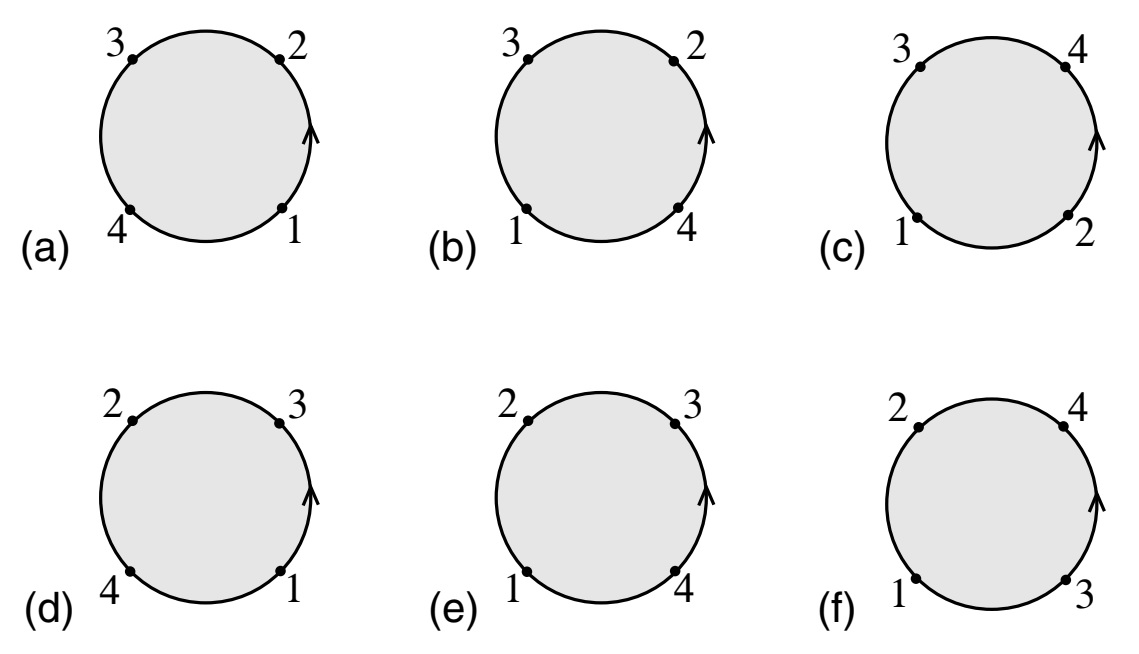
\includegraphics[width=0.5\textwidth]{figure/Fig6.2.jpg}\\
		\caption{Six cyclically inequivalent orderings of four open string vertex operators on a circle . Except for a jump from $\infty$ to $-\infty$ at point 3, the coordinate $y$ increases in the direction of the arrow .}\label{fig:6.2}
	\end{center}
\end{figure}


The integral splits into three parts, $-\infty<y_{4}<0$, $0<y_{4}<1$, and $1<y_{4}<\infty$ . For these three ranges, the ordering of vertex operators is as shown in figure \ref{fig:6.2}(a)(b)(c) . Möbius invariance can be used to transform these ranges to any other, so the contributions they give are equivalent to permutations of vertex operators . The $(t \leftrightarrow s)$ term gives figure \ref{fig:6.2}(d)(e)(f) . Taken together :
\begin{equation}
	S_{D_{2}}(k_{1} ; k_{2} ; k_{3} ; k_{4}=2 \mi g_{\mathrm{o}}^{4} C_{D_{2}}(2 \pi)^{26} \delta^{26}({\textstyle\sum_{i} k_{i}})
	[I(s, t)+I(t, u)+I(u, s)] \:, \label{6.4.9}
\end{equation}
where :
\begin{equation}
	I(s, t)=\int_{0}^{1} \dif y\: y^{-\alpha^{\prime} s-2}(1-y)^{-\alpha^{\prime} t-2}  \:. \label{6.4.10}
\end{equation}
These three terms come from figures \ref{fig:6.2} (c)(f), (b)(d), and (a)(e), respectively .

If $\alpha^{\prime} s<-1$ and $\alpha^{\prime} t<-1$, the integral $I(s,t)$ converges . As $\alpha^{\prime} s \rightarrow-1$, the integral diverges at $y=0$ . To study this divergence, take a neighborhood of $y=0$ and approximate the integrand :
\begin{align}
	I(s, t) &=\int_{0}^{r} d y y^{-\alpha^{\prime} s-2}+\text{terms analytic at } \alpha^{\prime} s=-1   \nonumber \\
	&=-\frac{r^{-\alpha^{\prime} s-1}}{\alpha^{\prime} s+1}+\text{terms analytic at } \alpha^{\prime} s=-1 \nonumber\\
	&=-\frac{1}{\alpha^{\prime} s+1}+\text{terms analytic at } \alpha^{\prime} s=-1 \:. \label{6.4.11}
\end{align}
In \eqref{6.4.11}, we calculated the integral in the convergence region . We see that this divergence is a pole at $s=-1 / \alpha^{\prime}$, the mass square of the open string tachyon . The variable $s$ is exactly the center-of-mass energy squared for the scattering $1+2 \rightarrow 3+4$, so this pole is a resonance produced by intermediate tachyon states . Once again, this is an artifact of the bosonic string, i.e., the lightest string state is a tachyon, which is irrelevant to the discussion . This pole is due to the process in figure \ref{fig:6.3}(a) . There, tachyons 1 and 2 merge into a single tachyon, then split back into tachyons 3 and 4 .

\begin{figure}[!htbp]
	\begin{center}
		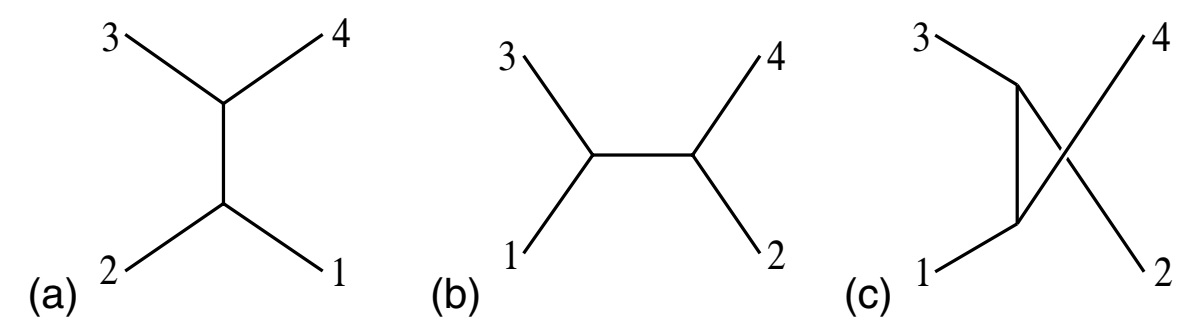
\includegraphics[width=0.5\textwidth]{figure/Fig6.3.jpg}\\
		\caption{Processes giving poles in the (a) $s$-, (b) $t$-, and (c) $u$-channels .}\label{fig:6.3}
	\end{center}
\end{figure}

Since the singularity at $\alpha^{\prime} s=-1$ is only a pole, $I(s,t)$ can be analytically continued around this point and into the region $\alpha^{\prime} s>-1$ . The amplitude is defined via analytic continuation . The divergence of the amplitude at this pole is a significant physical feature: the resonance corresponding to an intermediate string state propagating over long spacetime distances . Divergence bypassing this pole is not; it is merely an artifact of this specific integral representation of the amplitude . Continuation poses no problem . In fact, we will see that every string divergence is of this basic form, so this analytic continuation removes all divergences—except, of course, the divergence of the pole itself . The pole is on the real axis, and we need to define it more precisely . For Minkowski processes, the correct $\epsilon$ treatment is :
\begin{equation}
	\frac{1}{\alpha^{\prime} s+1}  \equiv \frac{1}{\alpha^{\prime} s+1+i \epsilon} 
	\equiv \mathrm{P} \frac{1}{\alpha^{\prime} s+1}- \mi \pi \delta (\alpha^{\prime} s+1) \:, \label{6.4.12}
\end{equation}
where $\mathrm{P}$ represents the principal value . Unitarity (which we will systematically develop in chapter \ref{cha:9}) requires this pole to appear, and determines the coefficient from the scattering amplitude of two tachyons to one string :
\begin{equation}
	S_{D_{2}}(k_{1} ; k_{2} ; k_{3} ; k_{4})= \mi \int \frac{\dif^{26} k}{(2 \pi)^{26}} 
	\frac{S_{D_{2}}(k_{1} ; k_{2} ; k) S_{D_{2}}(-k ; k_{3} ; k_{4})}{-k^{2}+\alpha^{\prime-1}+ \mi \epsilon} 
	+\text{ terms analytic at } k^{2}=\frac{1}{\alpha^{\prime}}\:. \label{6.4.13}
\end{equation}

Gathering factors in the 4-tachyon amplitude, including the equivalent contribution of $I(u, s)$ to this pole, and using the 3-tachyon result \eqref{6.4.4}, condition \eqref{6.4.13} gives :
\begin{equation}
	C_{D_{2}}=\me^{-\lambda} C_{D_{2}}^{X} C_{D_{2}}^{\mathrm{g}}=\frac{1}{\alpha^{\prime} g_{\mathrm{o}}^{2}} \:. \label{6.4.14}
\end{equation}
\begin{tcolorbox}
	\begin{remark}
		Singular term given by \eqref{6.4.13} :
		\[
		\mi \cdot(2 \mi g_{\mathrm{o}}^{3} C_{D_{2}})^{2}(2 \pi)^{26} \alpha^{\prime} 
		\delta^{2 b}({\textstyle\sum_{i} k_{i}}) \frac{1}{\alpha^{\prime} s+1} \:,
		\]
		Singular term given by \eqref{6.4.9} :
		\[
		2 \cdot 2 \mi g_{\mathrm{o}}^{4} C_{D_{2}}(2 \pi)^{26} \delta^{26}({\textstyle\sum_{i} k_{i}}) \frac{-1}{\alpha^{\prime} s+1}\:.
		\]
		The two together give \eqref{6.4.14} .
	\end{remark}
\end{tcolorbox}
\noindent Then the 3-tachyon amplitude is :
\begin{equation}
	S_{D_{2}}(k_{1} ; k_{2} ; k_{3})=\frac{2 \mi g_{\mathrm{o}}}{\alpha^{\prime}}(2 \pi)^{26} \delta^{26}({\textstyle\sum_{i} k_{i}}) \:. 
	\label{6.4.15}
\end{equation}
Various functional determinants are dropped . Using unitarity, all normalizations can be expressed in terms of the coupling $g_o$ appearing in vertex operators . In fact, the determinants can also be calculated through careful regularization and renormalization, and the relative normalization of different topologies is consistent with results derived from unitarity .

Continuing analytically around the pole, we encounter further singularities . Expanding the integrand at $y=0$ :
\begin{equation}
	I(s, t)=\int_{0}^{r} \dif y\: \Bigl[y^{-\alpha^{\prime} s-2}+ (\alpha^{\prime} t+2) y^{-\alpha^{\prime} s-1}+\cdots\Bigr] \:. \label{6.4.16}
\end{equation}
The second term gives the pole at $\alpha^{\prime} s=0$ :
\begin{equation}
	I(s, t)=\frac{u-t}{2 s}+\text{terms analytic at } \alpha^{\prime} s=0 \:. \label{6.4.17}
\end{equation}
From subsequent terms in the Taylor expansion, poles of the amplitude are at :
\begin{equation}
	\alpha^{\prime} s=-1,0,1,2, \ldots \:. \label{6.4.18}
\end{equation}
These are exactly the positions of open string states . The integral $I(s, t)$ has poles in variable $t$ at the same positions \eqref{6.4.18}, which come from endpoint $y=1$ . This is due to the process in figure \ref{fig:6.3}(b) . Other two terms in the amplitude \eqref{6.4.9} give poles in the $s$-, $t$-, and $u$-channels (figure \ref{fig:6.3}c) . Because the residue of \eqref{6.4.17} at $s=0$ is odd with respect to $u-t$, this pole will actually cancel with the pole in $I(s, u)$ . Singularities at even multiples of $1 / \alpha^{\prime}$ all exhibit this behavior . But for the more general open string theory introduced in the next section, this no longer holds . Defining the Euler beta function :
\begin{equation}
	B(a, b)=\int_{0}^{1} \dif y\: y^{a-1}(1-y)^{b-1} \:, \label{6.4.19}
\end{equation}
makes :
\begin{equation}
	I(s, t)=B(-\alpha_{\mathrm{o}}(s),-\alpha_{\mathrm{o}}(t)), \qquad \alpha_{\mathrm{o}}(x)=1+\alpha^{\prime} x \:. 
	\label{6.4.20}
\end{equation}
This can be expressed as gamma functions . For fixed $w$, define $y=v / w$, which gives :
\begin{equation}
	w^{a+b-1} B(a, b)=\int_{0}^{w} \dif v \: v^{a-1}(w-v)^{b-1} \:. \label{6.4.21}
\end{equation}
Multiplying both sides by $\me^{-w}$ and integrating $\int_{0}^{\infty} \dif w$, reassembling gives :
\begin{align}
	\Gamma(a+b) B(a, b) &=\int_{0}^{\infty} \dif v\: v^{a-1} \me^{-v} \int_{0}^{\infty} \dif(w-v) \: (w-v)^{b-1} \me^{-(w-v)} \nonumber \\
	&=\Gamma(a) \Gamma(b) \:. \label{6.4.22}
\end{align}
Then the 4-tachyon amplitude is :
\begin{align}
	&S_{D_{2}}(k_{1}; k_{2} ; k_{3} ; k_{4})=\frac{2 \mi g_{\mathrm{o}}^{2}}{\alpha^{\prime}}
	(2 \pi)^{26} \delta^{26}({\textstyle \sum_{i} k_{i}}) \nonumber \\
	&\qquad \times\Bigl[B(-\alpha_{\mathrm{o}}(s),-\alpha_{\mathrm{o}}(t))+B(-\alpha_{\mathrm{o}}(s),-\alpha_{\mathrm{o}}(u))
	+B(-\alpha_{\mathrm{o}}(t),-\alpha_{\mathrm{o}}(u))\Bigr] \:, \label{6.4.23}
\end{align}
where :
\begin{equation}
	B(-\alpha_{\mathrm{o}}(x),-\alpha_{\mathrm{o}}(y))=
	\frac{\Gamma(-\alpha^{\prime} x-1) \Gamma(-\alpha^{\prime} y-1)}{\Gamma(-\alpha^{\prime} x-\alpha^{\prime} y-2)} \:. \label{6.4.24}
\end{equation}
This is the Veneziano amplitude, originally written down to model certain features of strong interactions .

The high-energy behavior of the Veneziano amplitude is important . There are two interesting regions: the Regge limit ,
\begin{equation}
	s \rightarrow \infty, \quad t \text{ fixed} \:, \label{6.4.25}
\end{equation}
and the hard scattering limit :
\begin{equation}
	s \rightarrow \infty, \quad t / s \text{ fixed} \:. \label{6.4.26}
\end{equation}
If we consider the scattering process $1+2 \rightarrow 3+4$ (so that $k_{1}^{0}$ and $k_{2}^{0}$ are positive, and $k_{3}^{0}$ and $k_{4}^{0}$ are negative)  , then in the center-of-mass frame of $1$-$2$ :
\begin{equation}
	s=E^{2}, \quad t=(4 m^{2}-E^{2}) \sin^{2}\frac{\theta}{2}, \quad u=(4 m^{2}-E^{2}) \cos ^{2} \frac{\theta}{2} \:, \label{6.4.27}
\end{equation}
where $E$ is the center-of-mass frame energy, and $\theta$ is the angle between particles 1 and 3 . The Regge limit is high energy at a small angle, while the hard scattering limit is high energy at a fixed angle . Using Stirling's approximation, $\Gamma(x+1) \approx x^{x} \me^{-x}(2 \pi x)^{1 / 2}$, behavior in the Regge region is :
\begin{equation}
	S_{D_{2}}(k_{1} ; k_{2} ; k_{3} ; k_{4}) \propto s^{\alpha_{\mathrm{o}}(t)} \Gamma(-\alpha_{0}(t)) \:, \label{6.4.28}
\end{equation}
where $\alpha_{\mathrm{o}}(t)=\alpha^{\prime} t+1$, i.e., the amplitude varies as a power of $s$, where the power depends on $t$ . This is Regge behavior . At the poles of the gamma function, the amplitude is an integer power of $s$, corresponding to exchanging a string with integer spin $\alpha_o(t)$ .

In the hard scattering limit :
\begin{equation}
	S_{D_{2}}(k_{1} ; k_{2} ; k_{3} ; k_{4}) \approx \exp \bigl[-\alpha^{\prime}(s \ln s \alpha^{\prime}+t \ln t \alpha^{\prime}+u \ln u \alpha^{\prime})\bigr]=\exp [-\alpha^{\prime} s f(\theta)] \:, \label{6.4.29}
\end{equation}
where :
\begin{equation}
	f(\theta) \approx-\sin ^{2} \frac{\theta}{2} \ln \sin ^{2} \frac{\theta}{2}-\cos ^{2} \frac{\theta}{2} \ln \cos ^{2} \frac{\theta}{2}
	\label{6.4.30}
\end{equation}
is positive . \eqref{6.4.29} is noteworthy . High-energy, fixed-angle scattering probes the internal structure of the scattered objects . Rutherford discovered the atomic nucleus using hard $\alpha$ atom scattering . Hard electron-nucleon scattering at SLAC revealed the quark components of nucleons . In quantum field theory, hard scattering amplitudes decay according to a power law in $s$ . Even for a composite object like a nucleon, if its components are point-like, its amplitude follows a power law . The exponential decay \eqref{6.4.29} is much softer, reflecting an object with a size of $\alpha^{1 / 2}$, which is what we expect .

We started from 3-point amplitudes, skipping zero-, one-, and two-point amplitudes . We will discuss these amplitudes and their interpretations in section \ref{sec:6.6} .

\section{Chan-Paton factors and gauge interactions} \label{sec:6.5}

In this section, we will examine the interactions of massless vector states of the open string . To make this discussion more interesting, we first generalize the open string theory .

At the end of chapter \ref{cha:3}, we introduced a broad class of bosonic string theories, but in our preliminary examination of interactions, we focused on the simple case of 26-dimensional flat spacetime . We can think about it in terms of symmetry: this theory has a massive 26-dimensional Poincaré invariance . In the closed bosonic string, this is the only theory with this symmetry . The proof is summarized as follows: worldsheet Noether currents of spacetime translations have components with weights (1,0) and (0,1) . By the discussion given in section \ref{sec:2.9}, these currents are holomorphic with respect to $z$ or $\bar{z}$ . In calculations in this chapter, this is sufficient to determine all expectation values .

However, there exists a generalization in open string theory . Open strings have boundaries, endpoints . In quantum systems with distinguishable endpoints, it is natural to contain degrees of freedom at these points in addition to fields propagating in the bulk . At each endpoint of the open string, we add new degrees of freedom called Chan-Paton degrees of freedom, which can be one of $n$ states . Then the basis of string states is :
\begin{equation}
	|N ; k ; i j\rangle \:, \label{6.5.1}
\end{equation}
where $i$ and $j$ label the states of the left and right endpoints, ranging from 1 to $n$ . The energy-momentum tensor is defined as usual, with no dependence on the new degrees of freedom . Thus, conformal invariance is automatic . Since the Chan-Paton degrees of freedom are invariant, Poincaré invariance is also automatic . Although the worldsheet dynamics of these new degrees of freedom are trivial, they have profound implications for spacetime physics .

\begin{figure}[!htbp]
	\begin{center}
		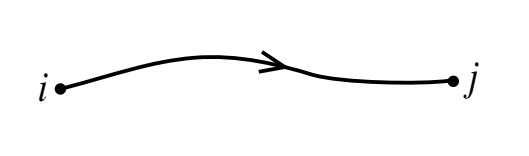
\includegraphics[width=0.5\textwidth]{figure/Fig6.4.jpg}\\
		\caption{An open string with Chan-Paton degrees of freedom .}\label{fig:6.4}
	\end{center}
\end{figure}

In the string theory of strong interactions, the motivation for introducing Chan-Paton factors was to introduce $SU(3)$ flavor quantum numbers: endpoints are like quarks and anti-quarks connected by a color-current tube . We now introduce it in a broader framework: consider all possible symmetries . In chapter \ref{cha:8}, we will give a new interpretation of Chan-Paton degrees of freedom, and in chapter 14, we will add a possible further improvement . Now there are $n^2$ scalar tachyons, $n^2$ massless vector bosons, and so on . Introduce $n^2$ Hermitian matrices $\lambda_{i j}^{a}$ and normalize as :
\begin{equation}
	\operatorname{Tr}(\lambda^{a} \lambda^{b})=\delta^{a b} \:, \label{6.5.2}
\end{equation}
These matrices are a complete basis for the states of the two endpoints . They are representation matrices of $U(n)$, so one can guess that the massless vector bosons are associated with $U(n)$ symmetry; we will soon see that this is indeed the case .

Define the basis :
\begin{equation}
	|N ; k ; a\rangle=\sum_{i, j=1}^{n}|N ; k ; i j\rangle \lambda_{i j}^{a}  \:. \label{6.5.3}
\end{equation}
Now consider the 4-tachyon amplitude shown in figure \ref{fig:6.2}(a), in which vertex operators are arranged in the cyclic order 1234 . Because Chan-Paton degrees of freedom do not appear in the Hamiltonian, their states cannot evolve between vertex operators: the state of the right endpoint of tachyon 1 must be the same as the state of the left endpoint of tachyon 2, and so on . Therefore, the amplitude in figure \ref{fig:6.2}(a) will contain the factor :
\begin{equation}
	\operatorname{Tr}(\lambda^{a_{1}} \lambda^{a_{2}} \lambda^{a_{3}} \lambda^{a_{4}}) \:, \label{6.5.4}
\end{equation}
which originates from the overlap of the Chan-Paton wavefunctions of each tachyon . This rule can be generalized to arbitrary amplitudes: each vertex operator now contains the Chan-Paton factor $\lambda_{i j}^{a}$ from the endpoint wavefunction, and the amplitude for each worldsheet is multiplied by the trace of Chan-Paton factors along the boundary . The 3-tachyon amplitude becomes :
\begin{align}
	S_{D_{2}}(k_{1}, a_{1} ; k_{2}, a_{2} ; k_{3}, a_{3})= 
	\frac{\mi g_{\mathrm{o}}}{\alpha^{\prime}}(2 \pi)^{26} \delta^{26}({\textstyle\sum_{i} k_{i}}) 
	\operatorname{Tr}(\lambda^{a_{1}} \lambda^{a_{2}} \lambda^{a_{3}}+\lambda^{a_{1}} \lambda^{a_{3}} \lambda^{a_{2}}) \:, \label{6.5.5}
\end{align}
The two cyclic orders now have different Chan-Paton traces . The 4-tachyon amplitude is :
\begin{align}
	&S_{D_{2}}(k_{1}, a_{1} ; k_{2}, a_{2} ; k_{3}, a_{3} ; k_{4}, a_{4})
	=\frac{\mi g_{\mathrm{o}}^{2}}{\alpha^{\prime}}(2 \pi)^{26} \delta^{26}({\textstyle \sum_{i} k_{i}}) \nonumber \\
	&\quad \times \Bigl[\operatorname{Tr}(\lambda^{a_{1}} \lambda^{a_{2}} \lambda^{a_{4}} \lambda^{a_{3}}
	+\lambda^{a_{1}} \lambda^{a_{3}} \lambda^{a_{4}} \lambda^{a_{2}}) B(-\alpha_{\mathrm{o}}(s),-\alpha_{\mathrm{o}}(t)) \nonumber  \\
	&\qquad+\operatorname{Tr}(\lambda^{a_{1}} \lambda^{a_{3}} \lambda^{a_{2}} \lambda^{a_{4}}
	+\lambda^{a_{1}} \lambda^{a_{4}} \lambda^{a_{2}} \lambda^{a_{3}}) B(-\alpha_{\mathrm{o}}(t),-\alpha_{\mathrm{o}}(u))\nonumber \\
	&\qquad+\operatorname{Tr}(\lambda^{a_{1}} \lambda^{a_{2}} \lambda^{a_{3}} \lambda^{a_{4}}
	+\lambda^{a_{1}} \lambda^{a_{4}} \lambda^{a_{3}} \lambda^{a_{2}}) 
	B(-\alpha_{\mathrm{o}}(s),-\alpha_{\mathrm{o}}(u))\Bigr] \:. \label{6.5.6}
\end{align}
Again considering the unitarity relation \eqref{6.4.13}, the pole at $s=-1 / \alpha^{\prime}$ gives the left side the factor :
\begin{equation}
	\frac{1}{4} \operatorname{Tr}\Bigl(\{\lambda^{a_{1}}, \lambda^{a_{2}}\} \{\lambda^{a_{3}}, \lambda^{a_{4}}\}\Bigr) \:,\label{6.5.7}
\end{equation}
while the right side gains the factor :
\begin{equation}
	\frac{1}{4} \sum_{a} \operatorname{Tr}\Bigl(\{\lambda^{a_{1}}, \lambda^{a_{2}}\} \lambda^{a}\Bigr) 
	\operatorname{Tr}\Bigl(\{\lambda^{a_{3}}, \lambda^{a_{4}}\} \lambda^{a}\Bigr) \:, \label{6.5.8}
\end{equation}
namely summing over the Chan-Paton wavefunctions of the intermediate states . The completeness and normalization \eqref{6.5.2} of $\lambda_{i j}^{a}$ imply that for any $A$ and $B$, one has :
\begin{equation}
	\operatorname{Tr}(A \lambda^{a}) \operatorname{Tr}(B \lambda^{a})=\operatorname{Tr}(A B) \:,  \label{6.5.9}
\end{equation}
thus the amplitude remains unitary .
\begin{tcolorbox}
	\begin{proof}
		Let $\operatorname{Tr}(A \lambda^{a})=\langle A \vert \lambda^{a}\rangle=\langle\lambda^{a}|A\rangle$, then :
		\[
		\operatorname{Tr}(A \lambda^{a}) \operatorname{Tr}(B \lambda^{a}) = 
		\langle A \vert \lambda^{a}\rangle\langle\lambda^{\alpha} \vert B\rangle=\langle A \vert B\rangle \:,
		\]
		where $\sum_{a}|\lambda^{a}\rangle\langle\lambda^{a}|=1$ comes from $\langle\lambda^{a} \vert \lambda^{b}\rangle= \delta^{a b}$ .
	\end{proof}	
\end{tcolorbox}



\subsection*{Gauge Interactions}
The amplitude of a gauge boson with two tachyons is :
\begin{align}
	&S_{D_{2}}(k_{1}, a_{1}, e_{1} ; k_{2}, a_{2} ; k_{3}, a_{3})= 
	-\mi g_{\mathrm{o}}^{\prime} g_{\mathrm{o}}^{2} \me^{-\lambda} e_{1 \mu} \nonumber \\
	&\quad \times\Bigl\langle \bno c^{1} \dot{X}^{\mu} \me^{\mi k_{1} \cdot X}(y_{1})\bno 
	\bno  c^{1} \me^{\mi k_{2} \cdot X}(y_{2})\bno \bno c^{1} \me^{\mi k_{3} \cdot X}(y_{3})\bno\Bigr\rangle_{D_{2}} 
	\operatorname{Tr}(\lambda^{a_{1}} \lambda^{a_{2}} \lambda^{a_{3}})  \nonumber\\
	&\qquad \qquad +(k_{2}, a_{2}) \leftrightarrow(k_{3}, a_{3}) \:. \label{6.5.10}
\end{align}
We use the bosonic vertex operator \eqref{3.6.26}, but temporarily allow an independent normalization constant $g_{\mathrm{o}}^{\prime}$ . Using the results from section \ref{sec:6.2}, the path integral of $X$ is :
\begin{align}
	&\Bigl\langle \bno \dot{X}^{\mu} \me^{\mi k_{1} \cdot X}(y_{1})\bno \bno \me^{\mi k_{2} \cdot X}(y_{2})\bno 
	\bno \me^{\mi k_{3} \cdot X}(y_{3})\bno \Bigr\rangle_{D_{2}} 
	=-2 \mi \alpha^{\prime}\biggl(\frac{k_{2}^{\mu}}{y_{12}}+\frac{k_{3}^{\mu}}{y_{13}}\biggr) \nonumber \\
	&\qquad \times \mi C_{D_{2}}^{X}(2 \pi)^{26} \delta^{26}({\textstyle \sum_{i} k_{i}})
	|y_{12}|^{2 \alpha^{\prime} k_{1} \cdot k_{2}}|y_{13}|^{2 \alpha^{\prime} k_{1} \cdot k_{3}} 
	|y_{23}|^{2 \alpha^{\prime} k_{2} \cdot k_{3}} \:. \label{6.5.11}
\end{align}
Using momentum conservation, mass-shell condition, and physical state condition $k_{1} \cdot e_{1}=0$, the amplitude becomes :
\begin{align}
	&S_{D_{2}}(k_{1}, a_{1}, e_{1} ; k_{2}, a_{2} ; k_{3}, a_{3}) \nonumber \\
	&=-\mi g_{\mathrm{o}}^{\prime} e_{1} \cdot k_{23}(2 \pi)^{26} \delta^{26}({\textstyle \sum_{i} k_{i}}) 
	\operatorname{Tr}\Bigl(\lambda^{a_{1}}[\lambda^{a_{2}}, \lambda^{a_{3}}]\Bigr) \:, \label{6.5.12}
\end{align}
where $k_{i j} \equiv k_{i}-k_{j}$ . This is again independent of the position of vertex operators .

The $s=0$ pole in the 4-tachyon amplitude is no longer zero . The term that was canceled now has Chan-Paton factors in a different order, so the pole is proportional to :
\begin{equation}
	\operatorname{Tr}\Bigl([\lambda^{a_{1}}, \lambda^{a_{2}}][\lambda^{a_{3}}, \lambda^{a_{4}}]\Bigr) \:. \label{6.5.13}
\end{equation}
Relating the coefficient of this pole to the amplitude \eqref{6.5.12} through unitarity gives :
\begin{equation}
	g_{\mathrm{o}}^{\prime}=(2 \alpha^{\prime})^{-1 / 2} g_{\mathrm{o}} \:. \label{6.5.14}
\end{equation}
This is the same as the relative normalization derived from the state-operator map: there is only one independent coupling constant . For the coupling of 3 gauge bosons, a similar calculation gives :
\begin{align}
	&S_{D_{2}}(k_{1}, a_{1}, e_{1} ; k_{2}, a_{2}, e_{2} ; k_{3}, a_{3}, e_{3}) \nonumber \\
	&\qquad = \mi g_{\mathrm{o}}^{\prime}(2 \pi)^{26} \delta^{26}({\textstyle\sum_{i} k_{i}})
	\Bigl(e_{1} \cdot k_{23} e_{2} \cdot e_{3}+e_{2} \cdot k_{31} e_{3} \cdot e_{1}+e_{3} \cdot k_{12} e_{1} \cdot e_{2} \nonumber\\
	&\qquad \qquad +\frac{\alpha^{\prime}}{2} e_{1} \cdot k_{23} e_{2} \cdot k_{31} e_{3} \cdot k_{12} \Bigr) 
	\operatorname{Tr}\Bigl(\lambda^{a_{1}}[\lambda^{a_{2}}, \lambda^{a_{3}}]\Bigr) \:. \label{6.5.15}
\end{align}

To first order in momentum, the amplitudes we found can be re-produced from the following spacetime action :
\begin{equation}
	\bm{S}=\frac{1}{g_{\mathrm{o}}^{\prime 2}} \int \dif^{26} x\: \biggl[-\frac{1}{2} \operatorname{Tr}(D_{\mu} \varphi D^{\mu}\varphi)+\frac{1}{2 \alpha^{\prime}} \operatorname{Tr}(\varphi^{2})+\frac{2^{1 / 2}}{3 \alpha^{\prime 1 / 2}} 
	\operatorname{Tr}(\varphi^{3})
	-\frac{1}{4} \operatorname{Tr}(F_{\mu \nu} F^{\mu \nu})\biggr] \:, \label{6.5.16}
\end{equation}
where the tachyon field $\varphi$ and the Yang-Mills vector potential $A_{\mu}$ are written as $n \times n$ matrices, i.e., $A_{\mu}=A_{\mu}^{a} \lambda^{a}$ . Furthermore, $D_{\mu} \varphi=\partial_{\mu} \varphi-\mi[A_{\mu}, \varphi]$, and $F_{\mu \nu}=\partial_{\mu} A_{\nu}-\partial_{\nu} A_{\mu}-\mi[A_{\mu}, A_{\nu}]$ .

This is the action for a $U(n)$ gauge field coupled to a scalar field in the adjoint representation . The addition of the Chan-Paton factor is exactly what is needed for the gauge-invariant representation . Since decoupling of non-physical states is guaranteed in string perturbation theory, gauge invariance is automatic, and we will study it further .

At momentum $k$ much smaller than the string scale, the only open string state is the massless gauge boson . As discussed in section \ref{sec:3.7}, in this limit, the physics should reduce to an effective field theory of massless states . Therefore, introducing the tachyon into the action \eqref{6.5.16} must be illogical in some places; we did so for heuristics . But now let us focus on the gauge boson . The form of the 4-gauge boson amplitude is similar to the Veneziano amplitude, but with extra structure from the polarization tensor . Expanding it as a power series in $\alpha^{\prime} k^{2}$, the first term survives in the zero-slope limit; it is the sum of pole terms in $s, t, u$ plus a constant . Consistency will guarantee that it is exactly the same as the 4-gauge boson amplitude obtained from the Yang-Mills Lagrangian $F_{\mu \nu} F^{\mu\nu}$ in field theory . Note, however, the term at order $\alpha^{\prime} k^{3}$ in the 3-gauge boson amplitude \eqref{6.5.15} . This implies higher-order derivative terms in the Lagrangian :
\begin{equation}
	-\frac{2 \mi \alpha^{\prime}}{3 g_{\text{o}}^{\prime 2}} \operatorname{Tr}(F_{\mu}{}^{\nu} F_{\nu}{}^{\omega} F_{\omega}{}^{\mu}) \:. \label{6.5.17}
\end{equation}
Similarly, expanding the 4-point amplitude will reveal an infinite sum of high-order interaction terms (besides \eqref{6.5.17}, they indeed have no kinematic contribution to the 3-gauge boson amplitude) . In low-energy regions, string loop amplitudes also reduce to loops obtained from the effective Lagrangian . By the general logic of effective Lagrangians, higher-order derivative terms are not very important at low energies  ; they become important at the scale $\alpha^{\prime} k^{2} \approx 1$, which is where new physics (massive string states) appears and the effective action is no longer applicable .

If we have a cutoff, why do we still need renormalization? Renormalization still has meaning . And in fact, this is its true interpretation: it means that low-energy physics is independent of the details of high-energy physics, except for the parameters in the effective Lagrangian . This is bittersweet: it means we can use ordinary quantum field theory to make predictions at accelerator energy levels without knowing the theory at the Planck scale, but it also means we cannot use physics at particle accelerators to probe the theory at the Planck scale .

String spectra and amplitudes have an obvious global $U(n)$ symmetry ,
\begin{equation}
	\lambda^{a} \rightarrow U \lambda^{a} U^{\dagger} \:, \label{6.5.18}
\end{equation}
which preserves the Chan-Paton trace and the norm of the states . From the details of the amplitudes, we see that this is actually local symmetry of spacetime . We will see that the elevation from global worldsheet symmetry to local spacetime symmetry is a very common phenomenon in string theory .

All open string states transform according to the $n \times n$ adjoint representation under $U(n)$ symmetry . Incidentally, $U(n)$ is not a simple Lie algebra: $U(n)=SU(n) \times U(1)$ . The $U(1)$ gauge boson, $\lambda_{i j}=\delta_{i j} / n^{1 / 2}$, decouples from amplitudes \eqref{6.5.12} and \eqref{6.5.15} . The adjoint representation of $U(1)$ is trivial, so all string states are neutral under $U(1)$ symmetry .

\subsection*{Non-orientable Strings}

The extension to non-orientable strings is interesting . First consider a theory without Chan-Paton factors . Besides Möbius invariance, the $X^{\mu}$ CFT on a sphere or disk is invariant under reflection symmetry in the direction of the open string $\sigma^{1} \rightarrow \pi-\sigma^{1}$ or on a closed string $\sigma^{1} \rightarrow 2 \pi-\sigma^{1}$ . Worldsheet parity is generated by the operator $\Omega$ . From the mode expansion, in open strings :
\begin{equation}
	\Omega \alpha_{n}^{\mu} \Omega^{-1}=(-1)^{n} \alpha_{n}^{\mu} \:, \label{6.5.19}
\end{equation}
and in closed strings :
\begin{equation}
	\Omega \alpha_{n}^{\mu} \Omega^{-1}=\tilde{\alpha}_{n}^{\mu} \:. \label{6.5.20}
\end{equation}
This symmetry also extends to ghost fields . But for concentration, we do not discuss them here; their contribution to tree-level diagrams is merely a fixed factor .

Regardless of whether it is an open or closed string, tachyon vertex operators are even under worldsheet parity (this is obvious for ghost-free integrated vertex operators; fixed operators must transform in the same way), which determines the sign of the operator . Then all states can be categorized according to their parity eigenvalues $\omega=\pm 1$ . The relation \eqref{6.5.19} in open strings implies :
\begin{equation}
	\Omega|N ; k\rangle=\omega_{N}|N ; k\rangle, \quad \omega_{N}=(-1)^{1+\alpha^{\prime} m^{2}} \:. \label{6.5.21}
\end{equation}
Worldsheet parity is multiplicative conservation . For example, the 3-tachyon amplitude is non-zero, consistent with $(+1)^{3}=1$ . On the other hand, massless vectors have $\omega=-1$, so we can expect the vector-tachyon-tachyon amplitude \eqref{6.5.10} and the 3-vector amplitude \eqref{6.5.15} to be zero in the absence of Chan-Paton factors, and this is indeed the case ($\lambda^{a}$ is replaced by 1, and the commutator is zero) . Different cyclic orders are also related to each other via worldsheet parity and thus cancel out .

Given a consistent oriented string theory, by restricting the spectrum to states with $\omega=+1$, we give a new non-orientable string theory . States where $\alpha^{\prime} m^{2}$ is odd are retained, while states where $\alpha^{\prime} m^{2}$ is even, including the photon, are forbidden . $\omega$ conservation guarantees that if all external states have $\omega=+1$, then intermediate states of tree-level diagrams also have $\omega=+1$ . Therefore, at least at the tree level, the unitarity of non-orientable strings follows from the unitarity of oriented strings .

The primary interest in non-orientable theory lies in the treatment of Chan-Paton factors . Since we can identify opposite endpoints of an open string, worldsheet parity must reverse them :
\begin{equation}
	\Omega|N ; k ; i j\rangle=\omega_{N}|N ; k ; j i\rangle \:. \label{6.5.22}
\end{equation}
Once again, this is a symmetry of all amplitudes in the oriented theory . To form a non-orientable theory, we again constrain the spectrum to worldsheet parity eigenvalues $\omega=+1$ . Take a set of basis for $\lambda_{i j}^{a}$ such that each matrix is either symmetric $s^{a}=+1$ or antisymmetric $s^{a}=-1$ . Then :
\begin{equation}
	\Omega|N ; k ; a\rangle=\omega_{N} s^{a}|N ; k ; a\rangle \:. \label{6.5.23}
\end{equation}
The worldsheet parity eigenvalue is $\omega=\omega_{N} s^{a}$, so the non-orientable spectrum is :
\begin{subequations} \label{6.5.24}
	\begin{align}
		&\text{even multiples of } \alpha^{\prime} m^{2} \:: \qquad   \text{antisymmetric } \lambda^{a}  \:, \label{6.5.24a} \\ 	
		&\text{odd multiples of } \alpha^{\prime} m^{2} \:: \qquad   \text{symmetric } \lambda^{a}  \:. \label{6.5.24b} 
	\end{align}			
\end{subequations}
For massless gauge bosons, Chan-Paton factors are $n \times n$ antisymmetric matrices, so the gauge group is $SO(n)$ . States at even mass levels transform according to the adjoint representation of the orthogonal group $SO(n)$, while states at odd mass levels transform according to a traceless symmetric tensor plus a singlet representation . The oriented theory has a large class of direction-reversing symmetries obtained as a combination of $\Omega$ and $U(n)$ rotations :
\begin{equation}
	\Omega_{\gamma}|N ; k ; i j\rangle=\omega_{N} \gamma_{j j^{\prime}}\left|N ; k ; j^{\prime} i^{\prime}\right\rangle \gamma_{i^{\prime} i}^{-1} \:. \label{6.5.25}
\end{equation}
By restricting the spectrum to $\omega_{y}=+1$, we can construct more general non-orientable theories . This is again compatible with interactions; applying $\Omega_{\gamma}$ twice gives :
\begin{equation}
	\Omega_{\gamma}^{2}|N ; k ; i j\rangle= [(\gamma^{T})^{-1} \gamma]_{i i^{\prime}} |N ; k ; i^{\prime} j^{\prime}\rangle (\gamma^{-1} \gamma^{T})_{j^{\prime} j} \:. \label{6.5.26}
\end{equation}
We assume $\Omega_{\gamma}^{2}=1$ for reasons explained below . This implies :
\begin{equation}
	\gamma^{T}=\pm \gamma \:. \label{6.5.27}
\end{equation}
That is, $\gamma$ is symmetric or antisymmetric .

The Chan-Paton basis transformation is :
\begin{equation}
	|N ; k ; i j\rangle^{\prime}=U_{i i^{\prime}}^{-1} |N ; k ; i^{\prime} j^{\prime}\rangle U_{j^{\prime} j} \:, \label{6.5.28}
\end{equation}
which changes $\gamma$ to :
\begin{equation}
	\gamma^{\prime}=U^{T} \gamma U \:. \label{6.5.29}
\end{equation}
In the symmetric case, one can always find a basis such that $\gamma=1$, which gives the case already examined above . In the antisymmetric case, there exists a basis such that :
\begin{equation}
	\gamma=M \equiv \mi\begin{bmatrix}
		0 & I \\
		-I & 0
	\end{bmatrix} \:. \label{6.5.30}
\end{equation}
Here $I$ is a $k \times k$ identity matrix; since $\gamma$ is an invertible antisymmetric matrix, $n=2 k$ must be even . We take a basis for the Chan-Paton wavefunctions such that $M(\lambda^{a})^{T} M=s^{a^{\prime}} \lambda^{a}$, where $s^{a^{\prime}}=\pm 1$ . Then the worldsheet eigenvalue is $\omega_{\gamma}=\omega_{N} s^{a^{\prime}}$, and the non-orientable spectrum is :
\begin{subequations} \label{6.5.31}
	\begin{align}
		\text{even multiples of } \alpha^{\prime} m^{2} \:: \qquad   M(\lambda^{a})^{T} M=-\lambda^{a} \:, \label{6.5.31a} \\
		\text{odd multiples of } \alpha^{\prime} m^{2} \:: \qquad   M(\lambda^{a})^{T} M=+\lambda^{a} \:. \label{6.5.31b}
	\end{align}
\end{subequations}
At even mass levels, including gauge bosons, this defines the adjoint representation of the symplectic group $Sp(k)$ .

To construct a non-orientable theory, we must have $\Omega_{\gamma}^{2}=1$ for the following reasons . Since $\Omega^{2}=1$, $\Omega_{\gamma}^{2}$ must only act on the Chan-Paton factors . In fact, from \eqref{6.5.26}, its action on the Chan-Paton wavefunction is :
\begin{equation}
	\lambda \rightarrow (\gamma^{T})^{-1} \gamma \lambda \gamma^{-1} \gamma^{T}=\lambda \:, \label{6.5.32}
\end{equation}
where, since all states are invariant under $\Omega_{\gamma}$, the last equal sign must hold in non-orientable theory . Now we assert that the allowed Chan-Paton wavefunctions must constitute a complete basis . The key is that two open strings can exchange endpoints through the split-aggregate interaction in figure \ref{fig:3.4}(c) . In this way, a complete basis, namely any Chan-Paton state $|i j\rangle$, can be reached . By Schur's Lemma, if \eqref{6.5.32} holds for the complete basis, then $\gamma^{-1} \gamma^{T}=1$, hence $\Omega_{\gamma}^{2}=1$ . By taking different sets of $\lambda^{a}$, we can try to obtain different gauge theories . In fact, the oriented $U(n)$ theory and non-orientable $SO(n)$ and $Sp(k)$ theories constructed above are the only possibilities . The extension of the completeness discussion in \eqref{6.5.7} -- \eqref{6.5.9} shows they are the most general solutions for non-orientable theories . In particular, exceptional Lie algebras cannot be obtained from Chan-Paton factors . In closed string theory, there are other mechanisms giving gauge bosons and allowing other groups .

\section{Closed string tree amplitudes} \label{sec:6.6}

The discussion of closed string amplitudes is similar to the above . The amplitude of 3 closed string tachyons is :
\begin{equation}
	S_{S_{2}}(k_{1} ; k_{2} ; k_{3})=g_{\mathrm{c}}^{3} \me^{-2 \lambda}\left\langle\prod_{i=1}^{3} : \mathrel{\tilde{c} c \me^{\mi k_{i} \cdot X}(z_{i}, \bar{z}_{i})}:\right\rangle \bigg._{\!\!S_{2}} \:. \label{6.6.1}
\end{equation}
In this case, the CKG $PSL(2, \mathds{C})$ (Möbius group) can fix three vertex operators at arbitrary positions $z_{1,2,3}$ . Taking the expectation value from section \ref{sec:6.2}, the result is again independent of the vertex operators :
\begin{equation}
	S_{S_{2}}(k_{1} ; k_{2} ; k_{3})= \mi g_{\mathrm{c}}^{3} C_{S_{2}}(2 \pi)^{26} \delta^{26}({\textstyle \sum_{i} k_{i}}) \:, \label{6.6.2}
\end{equation}
where $C_{S_{2}}=\me^{-2 \lambda} C_{S_{2}}^{X} C_{S_{2}}^{\mathrm{g}}$ .

For 4 closed string tachyons :
\begin{equation}
	S_{S_{2}}(k_{1} ; k_{2} ; k_{3} ; k_{4})=g_{\mathrm{c}}^{4} \me^{-2 \lambda} 
	\int_{\mathds{C}} \dif^{2} z_{4} \: \left\langle\prod_{i=1}^{3}
	: \mathrel{\tilde{c} c \me^{\mi k_{i} \cdot X}(z_{i}, \bar{z}_{i})}:
	: \mathrel{\me^{\mi k_{4} \cdot X}(z_{4}, \bar{z}_{4})}:\right\rangle\bigg._{\!\!S_{2}} \:, \label{6.6.3}
\end{equation}
where the integral range is the entire complex plane $\mathds{C}$ . Calculating the expectation value and letting $z_{1}=0, z_{2}=1, z_{3}=\infty$, this becomes :
\begin{equation}
	S_{S_{2}}(k_{1} ; k_{2} ; k_{3} ; k_{4}) = 
	\mi g_{\mathrm{c}}^{4} C_{S_{2}}(2 \pi)^{26} \delta^{26}({\textstyle\sum_{i} k_{i}}) J(s, t, u) \:, \label{6.6.4}
\end{equation}
where :
\begin{equation}
	J(s, t, u)=\int_{\mathds{C}} \dif^{2} z_{4}\: |z_{4}|^{-\alpha^{\prime} u / 2-4}|1-z_{4}|^{-\alpha^{\prime} t/2-4}\:. \label{6.6.5}
\end{equation}
Here $s+t+u=-16 / \alpha^{\prime}$; we have labeled here the correlation of $J$ with all 3 variables to emphasize their symmetry . When $s, t, u<-4 / \alpha^{\prime}$, the amplitude converges . As $z_{4} \rightarrow 0$, it has a pole with respect to $u$; as $z_{4} \rightarrow 1$, it has a pole with respect to $t$; as $z_{4} \rightarrow \infty$, it has a pole with respect to $s$ . These poles are at :
\begin{equation}
	\alpha^{\prime} s\,,\: \alpha^{\prime} t \,,\: \alpha^{\prime} u=-4,0,4,8, \ldots,\label{6.6.6}
\end{equation}
which are the mass squared of closed string states . The pole at $\alpha^{\prime} s=-4$ is :
\begin{equation}
	\mi g_{\mathrm{c}}^{4} C_{S_{2}} \int_{|z_{4}|>1 / \epsilon} \dif^{2} z_{4}\: |z_{4}|^{\alpha^{\prime} s / 2} 
	\sim-\frac{8 \pi \mi g_{\mathrm{c}}^{4} C_{S_{2}}}{\alpha^{\prime} s+4} \:. \label{6.6.7}
\end{equation}
Unitarity gives :
\begin{equation}
	C_{S_{2}}=\frac{8 \pi}{\alpha^{\prime} g_{\mathrm{c}}^{2}} \:, \label{6.6.8}
\end{equation}
therefore :
\begin{equation}
	S_{S_{2}}(k_{1} ; k_{2} ; k_{3})=\frac{8 \pi \mi g_{\mathrm{c}}}{\alpha^{\prime}}(2 \pi)^{26} 
	\delta^{26}({\textstyle\sum_{i} k_{i}}) \:. \label{6.6.9}
\end{equation}

Similar to the Veneziano amplitude, the 4-closed-string-tachyon amplitude can be expressed as gamma functions :
\begin{equation}
	S_{S_{2}}(k_{1} ; k_{2} ; k_{3} ; k_{4})=\frac{8 \pi \mi g_{\mathrm{c}}^{2}}{\alpha^{\prime}}(2 \pi)^{26} 
	\delta^{26}({\textstyle \sum_{i} k_{i}}) C(-\alpha_{\mathrm{c}}(t),-\alpha_{\mathrm{c}}(u)) \:, \label{6.6.10}
\end{equation}
where $\alpha_{\mathrm{c}}(x)=1+\alpha^{\prime} x / 4$ and :
\begin{align}
	C(a, b) &=\int_{\mathds{C}} \dif^{2} z \: |z|^{2 a-2}|1-z|^{2 b-2} \nonumber \\
	&=2 \pi \frac{\Gamma(a) \Gamma(b) \Gamma(c)}{\Gamma(a+b) \Gamma(a+c) \Gamma(b+c)}\:, \quad a+b+c=1 \:. \label{6.6.11}
\end{align}
This is the Virasoro-Shapiro amplitude . There is only one term, and the poles in the $s, t, u$ channels come from the gamma functions in the numerator . Similar to the Veneziano amplitude, the Virasoro-Shapiro amplitude exhibits Regge behavior in the Regge limit :
\begin{equation}
	S_{S_{2}}(k_{1} ; k_{2} ; k_{3} ; k_{4}) \propto s^{2 \alpha_{\mathrm{c}}(t)} 
	\frac{\Gamma(-\alpha_{\mathrm{c}}(t))}{\Gamma(1+\alpha_{\mathrm{c}}(t))} \:, \label{6.6.12}
\end{equation}
and exponential behavior in the hard scattering limit :
\begin{equation}
	S_{S_{2}}(k_{1} ; k_{2} ; k_{3} ; k_{4}) \propto \exp 
	\biggl[-\frac{\alpha^{\prime}}{2}(s \ln s \alpha^{\prime}+t \ln t \alpha^{\prime}+u \ln u \alpha^{\prime})\biggr] \:. \label{6.6.13}
\end{equation}

On the sphere, the amplitude for one massless closed string and two closed string tachyons is :
\begin{align}
	S_{S_{2}}(k_{1}, e_{1} ; k_{2} ; k_{3}) &= g_{\mathrm{c}}^{2} g_{\mathrm{c}}^{\prime} 
	\me^{-2 \lambda} e_{1 \mu \nu} \Biggl\langle: \mathrel{\tilde{c} c \partial X^{\mu} \bar{\partial} X^{\nu} 
		\me^{\mi k_{1} \cdot X}(z_{1}, \bar{z}_{1})}: \nonumber \\
	&\qquad \qquad \quad : \mathrel{\tilde{c} c \me^{\mi k_{2} \cdot X}(z_{2}, \bar{z}_{2})}:
	: \mathrel{\tilde{c} c \me^{\mi k_{3} \cdot X}(z_{3}, \bar{z}_{3})}: \biggr\rangle_{S_{2}}  \nonumber \\
	& =-\frac{\pi \mi \alpha^{\prime}}{2} g_{\mathrm{c}}^{\prime} e_{1 \mu \nu} k_{23}^{\mu} k_{23}^{\nu}
	(2 \pi)^{26} \delta^{26}({\textstyle\sum_{i} k_{i}}) \:, \label{6.6.14}
\end{align}
where $e_{1 \mu \nu} e_{1}^{\mu \nu}=1$ . Expanding the Virasoro-Shapiro amplitude \eqref{6.6.10} at the $s=0$ pole, unitarity can give :
\begin{equation}
	g_{\mathrm{c}}^{\prime}=\frac{2}{\alpha^{\prime}} g_{\mathrm{c}} \:, \label{6.6.15}
\end{equation}
which is again consistent with the state-operator map containing the overall constant $g_{\mathrm{c}}$ . The amplitude \eqref{6.6.14} can be obtained from field theory via the action $\bm{S}+\bm{S}_{T}$, where $\bm{S}$ is the action for massless fields \eqref{3.7.20}, and :
\begin{equation}
	\bm{S}_{T}=-\frac{1}{2} \int \dif^{26} x\: (-G)^{1 / 2} \me^{-2 \tilde{\Phi}}
	\biggl(G^{\mu \nu} \partial_{\mu} T \partial_{\nu} T-\frac{4}{\alpha^{\prime}} T^{2} \biggr) \:, \label{6.6.16}
\end{equation}
which is the action for a closed string tachyon $T$ . For example, the graviton amplitude with polarization $e_{\mu \nu}$ can be obtained by expanding :
\begin{equation}
	\tilde{G}_{\mu \nu}=\eta_{\mu \nu}-2 \kappa e_{\mu \nu} \me^{\mi k \cdot x} \:, \label{6.6.17}
\end{equation}
from this action . Note that this is the Einstein metric, and its action \eqref{3.7.25} does not contain the dilaton . The normalization of the fluctuation is determined by the fluctuation of the graviton kinetic energy term in the spacetime action . Specifically, if taking $\tilde{G}_{\mu \nu}-\eta_{\mu \nu}=-2 \kappa e_{\mu \nu} f(x)$ where $e_{\mu \nu} e^{\mu \nu}=1$, the effective action of $f$ has the canonical normalization $\frac{1}{2}$ for real scalars . The field theory amplitude matches the string theory result \eqref{6.6.14} and relates to the normalization of the gravitational coupling vertex operator :
\begin{equation}
	\kappa=\pi \alpha^{\prime} g_{\mathrm{c}}^{\prime}=2 \pi g_{\mathrm{c}} \:. \label{6.6.18}
\end{equation}

The 3-massless-closed-string amplitude is :
\begin{equation}
	S_{S_{2}}(k_{1}, e_{1} ; k_{2}, e_{2} ; k_{3}, e_{3})=\frac{\mi \kappa}{2}(2 \pi)^{26} 
	\delta^{26}(\textstyle{\sum_{i} k_{i}}) e_{1 \mu \nu} e_{2 \alpha \beta} e_{3 \gamma \delta} T^{\mu \alpha \gamma} T^{\nu \beta \delta} \:, \label{6.6.19}
\end{equation}
where :
\begin{equation}
	T^{\mu \alpha \gamma}=k_{23}^{\mu} \eta^{\alpha \gamma}+k_{31}^{\alpha} \eta^{\gamma \mu}+k_{12}^{\gamma} \eta^{\mu \alpha}+\frac{\alpha^{\prime}}{8} k_{23}^{\mu} k_{31}^{\alpha} k_{12}^{\gamma} \:. \label{6.6.20}
\end{equation}
The $k^2$ term of this amplitude corresponds to the spacetime action \eqref{3.7.25}, while the $k^4$ and $k^6$ terms come from several high-order derivative interactions, including terms of order 2 and 3 in the spacetime curvature . Higher-order corrections to the action can also be obtained by calculating high-loop corrections of the worldsheet $\beta$ function \eqref{3.7.14} .

If we set $\alpha^{\prime}=\frac{1}{2}$ for open strings and $\alpha^{\prime}=2$ for closed strings, the tensor structure of the closed string amplitude \eqref{6.6.19} is just two copies of the open string amplitude \eqref{6.5.15} . The same result holds for the amplitude \eqref{6.6.14} . This is the result of the free-field expectation values on the sphere factorizing into holomorphic and anti-holomorphic parts . Similar factorization occurs for four or more closed strings before integrating over the vertex operator positions . Furthermore, through careful treatment of the integration contours, it is possible to find relations between the integrated amplitudes . For 4-tachyon amplitudes, after using $\Gamma(x) \Gamma(1-x) \sin (\pi x)=\pi$, the above integrals have the following relationship :
\begin{equation}
	J(s, t, u, \alpha^{\prime})=-2 \sin \pi \alpha_{\mathrm{c}}(t) I(s, t, 4 \alpha^{\prime}) I(t, u, 4 \alpha^{\prime}) \:; \label{6.6.21}
\end{equation}
we have now indicated the explicit correlation of the integral for $\alpha^{\prime}$ . For the general integral appearing in 4-point closed string amplitudes, there is the following relationship :
\begin{align}
	&\int_{\mathds{C}} \dif^{2} z\: z^{a-1+m_{1}} \bar{z}^{a-1+n_{1}}(1-z)^{b-1+m_{2}}(1-\bar{z})^{b-1+n_{2}} \nonumber \\
	&\qquad =2 \sin [\pi(b+n_{2})] B(a+m_{1}, b+m_{2}) B(b+n_{2}, 1-a-b-n_{1}-n_{2}) \:. \label{6.6.22}
\end{align}
This implies the relationship between 4-point open string amplitudes and 4-point closed string amplitudes :
\begin{equation}
	A_{\mathrm{c}}(s, t, u, \alpha^{\prime}, g_{\mathrm{c}}) = 
	\frac{\pi \mi g_{\mathrm{c}}^{2} \alpha^{\prime}}{g_{\mathrm{o}}^{4}} 
	\sin [\pi \alpha_{\mathrm{c}}(t)] A_{\mathrm{o}}(s, t, \tfrac{1}{4} \alpha^{\prime}, g_{\mathrm{o}}) 
	A_{\mathrm{o}}(t, u, \tfrac{1}{4} \alpha^{\prime}, g_{\mathrm{o}})^{*} \:, \label{6.6.23}
\end{equation}
where the open string amplitude contains only one of the 6 cyclic orderings, and the pole is in the stated channel .

\subsection*{Consistency}
In chapter \ref{cha:9}, we will discuss convergence and gauge invariance of tree-level amplitudes in a general way, but as an introduction, we now first use OPE to see how this works at the lowest order . Examine the operator product :
\begin{align}
	&: \mathrel{\me^{\mi k_{1} \cdot X(z_{1}, \bar{z}_{1})}}: 
	: \mathrel{\me^{\mi k_{4} \cdot X(z_{4}, \bar{z}_{4})}}: = 
	|z_{14}|^{\alpha^{\prime} k_{1} \cdot k_{4}}:\!\!
	\Bigl(1+ \mi z_{14} k_{1} \cdot \partial X + \mi \bar{z}_{14} k_{1} \cdot \bar{\partial} X \nonumber \\
	&\qquad \qquad -z_{14} \bar{z}_{14} k_{1} \cdot \partial X k_{1} \cdot \bar{\partial} X+\cdots \Bigr) 
	\,\me^{\mi(k_{1}+k_{4}) \cdot X}(z_{4}, \bar{z}_{4})\!\!: \:. \label{6.6.24}
\end{align}
It appears in amplitudes where $z_{14}$ is integrated out . When :
\begin{equation}
	\alpha^{\prime} k_{1} \cdot k_{4}=\frac{\alpha^{\prime}}{2}(k_{1}+k_{4})^{2}-4>-2 \:, \label{6.6.25}
\end{equation}
the integral converges at $z_{14} \rightarrow 0$, and it has a pole at $-2$ . The coefficient of this pole is the tachyon vertex operator . Therefore, in any amplitude, if a pair of tachyons has total momentum $(k_{1}+k_{4})^{2}=4 / \alpha^{\prime}$, there will be a pole, and unitarity requires this pole to be proportional to the amplitude with one fewer tachyon . Poles in momentum space correspond to long distances in spacetime, so this is a process where two tachyons scatter into one tachyon, which then interacts with other particles . Further doing OPE, the $O(z_{14})$ and $O(\bar{z}_{14})$ terms do not produce tachyons because the angular integration gives zero residue, and $O(z_{14} \bar{z}_{14})$ gives massless poles, and so on . Now we study more closely how local spacetime symmetry is maintained in string amplitudes . If any polarization vector is of the form $e_{\mu}=k_{\mu}$, or $e_{\mu \nu}=\zeta_{\mu} k_{\nu}+k_{\mu} \tilde{\zeta}_{\mu}$, where $k \cdot \zeta=k \cdot \tilde{\zeta}=0$, the scattering amplitudes we calculated are all zero . This corresponds to the action being invariant under Yang-Mills, coordinate, and antisymmetric tensor symmetries . As discussed in section \ref{sec:3.6}, the vertex operator of longitudinal polarization is the sum of a full derivative and another term, which is zero due to the equations of motion . After integration, the full derivative term is zero, but the equations of motion term may have sources at other vertex locations in the path integral . When $k_{1} \cdot k_{4}$ is large, the operator product \eqref{6.6.24} decreases rapidly to zero . Using this property, for any pair of operators, there will always be a kinematic region where all possible connected terms (contact) are suppressed . Then the amplitude of null polarization is identically zero in this region because all amplitudes except at poles are analytic; the amplitude of null polarization must be zero everywhere . We see that the poles required by unitarity and the destruction of all possible divergences and spacetime gauge invariance arise in the limits $z \rightarrow 0,1, \infty$ and when two vertex operators approach each other . For a sphere with 4 marked points, they are the boundaries of the moduli space . For historical reasons, the analytic continuation discussion here is called the canceled propagator argument .

\subsection*{Closed Strings on $D_{2}$ and $RP_{2}$}
Lowest-order closed-string-open-string interactions come from disks having both closed string vertex operators and open string vertex operators . Their low-energy effective actions can be derived from a general discussion . In a trivial closed string background, we find the usual gauge kinetic term ,
\begin{equation}
	-\frac{1}{4 g_{\mathrm{o}}^{\prime 2}} \int \dif^{26} x\: \operatorname{Tr}(F_{\mu \nu} F^{\mu \nu}) \:. \label{6.6.26}
\end{equation}
Clearly the metric must be coupled to it in a covariant way . In addition, coupling with the dilaton can be derived . Recall $g_{\mathrm{o}}^{\prime 2} \propto \me^{\Phi_{0}}$, where $\Phi_{0}$ is the expectation value of the dilaton . So we replace it again (inside the integral) with $\Phi=\Phi_{0}+\tilde{\Phi}$ . The action :
\begin{equation}
	-\frac{1}{4 g_{\mathrm{o}}^{\prime 2}} \int \dif^{26} x \: (-G)^{1/2} \me^{-\tilde{\Phi}} \operatorname{Tr}(F_{\mu \nu} F^{\mu \nu}) \label{6.6.27}
\end{equation}
contains all interactions except for derivatives of the closed string field . Indices are now raised and lowered with $G_{\mu \nu}$ . This action reflects the property that the effective action from Euler number $\chi$ contains weight $g_{\mathrm{c}}^{-\chi} \propto \me^{-\chi \Phi}$ .

The disk and projective plane also contribute to pure closed string interactions . The amplitude of $n$ closed strings is of order $g_{\mathrm{o}}^{-2} g_{\mathrm{c}}^{n} \sim g_{\mathrm{c}}^{n-1}$, one $g_{\mathrm{c}}$ more than the sphere . For closed string loop amplitudes considered in the next section, since emitting or absorbing a closed string adds 2 $g_{\mathrm{c}}$ factors, it is $g_{\mathrm{c}}^{2}$ times the sphere . Therefore the sphere and the projective plane are at the "half-loop order" .

One of the most interesting amplitudes on the sphere and the projective plane is the one containing a single closed string vertex operator . Fixing the position of the vertex operator removes only two of the three CKVs; the residual gauge transformation consists of a rotation about the vertex operator position . Therefore, the scattering amplitude must be divided by the volume of the residual CKG . We have not yet explicitly proven it, but the torus in the next chapter will solve this problem . For a disk with one closed string, this is a finite and non-zero factor . The amplitude is a numerical factor times $g_{\mathrm{c}} g_{\mathrm{o}}^{-2}$, which is a pure number, multiplied by powers of $\alpha^{\prime}$ (from dimensional analysis) . We will not solve for these numerical factors here, but will obtain them indirectly in chapter \ref{cha:8} .

Therefore, for closed strings emerging from a vacuum (momentum zero), there is an amplitude from both the disk and the projective plane; this type of amplitude is called a tadpole amplitude . In other words, the background closed string fields would be corrected to order $g_{\mathrm{c}}$ from their initial values . We can also write the effective action :
\begin{equation}
	-\Lambda \int \dif^{26} x \: (-G)^{1/2} \me^{-\tilde{\Phi}} \:, \label{6.6.28}
\end{equation}
which is the potential for the dilaton, which we will further examine in the next chapter .

On the other hand, for a single closed string on the sphere, the amplitude is zero . The residual CKG is the non-compact subgroup of $PSL(2, \mathds{C})$, and thus this amplitude is divided by an infinite volume . A non-zero result would have logical inconsistency, i.e., zero-order correction to the background field . Similarly, the two-closed-string amplitude on the sphere (zero-order correction to mass) is also zero . For the corresponding disk amplitude, when there are one or two open strings, it is also zero . Amplitudes without vertex operators are also meaningful—they happen to calculate the $\tilde{\Phi}^{0}$ order term in the Taylor expansion of the action \eqref{6.6.28} . A disk without vertex operators is therefore not zero, which requires a formal treatment of the conformal Killing volume .

\section{General results}  \label{sec:6.7} 

In this section, we will obtain some general results for CFT on spheres and disks .

\subsection*{Möbius Invariance}
We have seen that there is a globally defined group of conformal transformations on the sphere, the Möbius group $PSL(2, \mathds{C})$ :
\begin{equation}
	z^{\prime}=\frac{\alpha z+\beta}{\gamma z+\delta} \:, \label{6.7.1}
\end{equation}
where $\alpha, \beta, \gamma, \delta$ are complex numbers satisfying $\alpha \delta-\beta \gamma=1$ . This is the most general one-to-one conformal transformation on the sphere $S_2$ . Expectation values must be invariant under any Möbius transformation :
\begin{equation}
	\bigl\langle\mathscr{A}_{i}(z_{1}, \bar{z}_{1}) \ldots \mathscr{A}_{k}(z_{n}, \bar{z}_{n})\bigr\rangle_{S_{2}} =
	\bigl\langle\mathscr{A}_{i}^{\prime}(z_{1}, \bar{z}_{1}) \ldots \mathscr{A}_{k}^{\prime}(z_{n}, \bar{z}_{n})\bigr\rangle_{S_{2}} \:. \label{6.7.2}
\end{equation}
We will examine the consequences of this symmetry for 1, 2, 3, and 4 local operators .

For a single operator with weight $(h_{i}, \tilde{h}_{i})$, rescaling plus rotation $z^{\prime}=\gamma z$ gives :
\begin{equation}
	\bigl\langle\mathscr{A}_{i}(0,0)\bigr\rangle_{S_{2}} = \bigl\langle\mathscr{A}_{i}^{\prime}(0,0)\bigr\rangle_{S_{2}}
	=\gamma^{-h_{i}} \bar{\gamma}^{-\tilde{h}_{i}}\bigl\langle\mathscr{A}_{i}(0,0)\bigr\rangle_{S_{2}} \:. \label{6.7.3}
\end{equation}
Therefore, unless $h_{i}=\tilde{h}_{i}=0$, the one-point function is zero . Since the matter factor is the expectation value of the $(1,1)$ operator, this is another way to see that the one-point amplitude is zero on the sphere .

When $n=2$, we can use translation plus $z^{\prime}=\gamma z$ to move any pair of operators to positions 0 and 1, giving :
\begin{equation}
	\bigl\langle\mathscr{A}_{i}(z_{1}, \bar{z}_{1}) \mathscr{A}_{j}(z_{2}, \bar{z}_{2})\bigr\rangle_{S_{2}}
	=z_{12}^{-h_{i}-h_{j}} \bar{z}_{12}^{-\tilde{h}_{i}-\tilde{h}_{j}}
	\bigl\langle\mathscr{A}_{i}(1,1) \mathscr{A}_{j}(0,0)\bigr\rangle_{S_{2}} \:, \label{6.7.4}
\end{equation}
so the position dependence is completely determined . Singularity implies $J_{i}+J_{j} \in \mathds{Z}$, where $J_{i}=h_{i}-\tilde{h}_{i}$ .
\begin{tcolorbox}
	\begin{remark}
		$J_{i}+J_{j}=(h_{i}+h_{j})-(\tilde{h}_{i}+\tilde{h}_{j})$, so $z_{12} \rightarrow \me^{\mi \theta} z_{12}$, $\bar{z}_{12}\rightarrow \me^{-\mi \theta} \bar{z}_{12}$ .
	\end{remark}
\end{tcolorbox}
\noindent Conformal transformation $z^{\prime}=z+\epsilon(z-z_{1})(z-z_{2})+O(\epsilon^{2})$ puts further constraints on the two-point function, keeping $z_1$ and $z_2$ fixed . For general operators this is complex, but for tensor fields $\mathcal{O}_{p}$ and $\mathcal{O}_{q}$, it implies :
\begin{equation}
	\text{unless}\:\: h_{p}=h_{q}, \quad \tilde{h}_{p}=\tilde{h}_{q}\:, \qquad 
	\bigl\langle\mathcal{O}_{p}(z_{1}, \bar{z}_{1}) \mathcal{O}_{q}(z_{2}, \bar{z}_{2})\bigr\rangle_{S_{2}}=0 \:. \label{6.7.5}
\end{equation}

By Möbius transformations, any three points $z_{1,2,3}$ can be brought to specific positions . When $n \geq 3$, Möbius invariance thus reduces expectation values from functions of $n$ complex variables to functions of $n-3$ variables . Again, this result takes a simple form only for tensor fields . For example, for three tensor fields :
\begin{equation}
	\left\langle\prod_{i=1}^{3} \mathcal{O}_{p_{i}}(z_{i}, \bar{z}_{i})\right\rangle\bigg._{\!\!S_{2}}
	=C_{p_{1} p_{2} p_{3}} 
	\prod_{i<j}^{3} z_{i j}^{h-2(h_{i}+h_{j})} \bar{z}_{i j}^{\tilde{h}-2(\tilde{h}_{i}+\tilde{h}_{j})} \:, \label{6.7.6}
\end{equation}
where $C_{p_{1} p_{2} p_{3}}$ is independent of position, and $h=h_{1}+h_{2}+h_{3}$ . For four primary fields :
\begin{equation}
	\left\langle\prod_{i=1}^{4} \mathcal{O}_{p_{i}}(z_{i}, \bar{z}_{i})\right\rangle\bigg._{\!\!S_{2}}
	=C_{p_{1} p_{2} p_{3} p_{4}}(z_{c}, \bar{z}_{c}) \, (z_{12} z_{34})^{h}(\bar{z}_{12} \bar{z}_{34})^{\tilde{h}} \times 
	\prod_{i<j}^{4} z_{i j}^{-h_{i}-h_{j}} \bar{z}_{i j}^{-\tilde{h}_{i}-\tilde{h}_{j}} \:, \label{6.7.7}
\end{equation}
where $h=\sum_{i} h_{i}$, $\tilde{h}=\sum_{i} \tilde{h}_{i}$, and $z_{c}=z_{12} z_{34} / z_{13} z_{24}$ is the Möbius-invariant cross ratio . The function $C_{p_{1} p_{2} p_{3} p_{4}}(z_{c}, \bar{z}_{c})$ is not determined by conformal invariance, so we reduced the function of four variables to a function of a single variable .

On a disk represented as a half-plane, only Möbius transformations with real $\alpha, \beta, \gamma, \delta$ are retained, constituting the group $PSL(2, \mathds{R})$ . By examining the complete conformal algebra, we will gain more information . We will see in chapter 15 that it will determine all expectation values in terms of these tensor fields .

\subsection*{Path Integrals and Matrix Elements}
Path integrals we have considered can be linked with operator representations . Consider the path integral for two operators on a sphere, one at the origin and one at infinity :
\begin{equation}
	\bigl\langle\mathscr{A}_{i}^{\prime}(\infty, \infty) \mathscr{A}_{j}(0,0)\bigr\rangle_{S_{2}} \:. \label{6.7.8}
\end{equation}
Primed labels denote the $u$ coordinate system, which must be taken for operators at infinity; with slight ambiguity of notation, we can still represent position in terms of $z$ . Using the state-operator map, one can replace the disk $|z|<1$ containing $\mathscr{A}_{j}$ with the state $\Psi_{\mathscr{A}_{j}}$ on circle $|z|=1$ . We can also replace the disk $|z|>1$ containing $\mathscr{A}_{i}$ with the state $\Psi_{\mathscr{A}_{i}}$ on circle $|z|=1$ . So the expectation value \eqref{6.7.8} becomes :
\begin{equation}
	\int[\dif \phi_{\mathrm{b}}]\: \Psi_{\mathscr{A}_{i}}[\phi_{\mathrm{b}}^{\Omega}] 
	\Psi_{\mathscr{A}_{j}}[\phi_{\mathrm{b}}] \:; \label{6.7.9}
\end{equation}
where $\phi_{\mathrm{b}}^{\Omega}(\sigma)=\phi_{\mathrm{b}}(2 \pi-\sigma)$, from mapping $z u=1$ .

This inner product of wavefunctions is similar to an inner product, so we define :
\begin{equation}
	\lAngle i \vert j\rangle = \bigl\langle\mathscr{A}_{i}^{\prime}(\infty, \infty) \mathscr{A}_{j}(0,0)\bigr\rangle_{S_{2}} \:. \label{6.7.10}
\end{equation}
This inner product was introduced by Zamolodchikov . For a unitary operator in a unitary theory, Möbius transformations show it is the same as the coefficient of 1 in the OPE :
\begin{equation}
	\mathcal{O}_{i}(z, \bar{z}) \mathcal{O}_{j}(0,0)=\frac{\lAngle i \vert j\rangle}{z^{h_{i}+h_{j}} \bar{z}^{\tilde{h}_{i}+\tilde{h}_{j}}\langle 1\rangle_{S_{2}}}+\cdots \:. \label{6.7.11}
\end{equation}
We abbreviate $|\mathscr{A}_{i}\rangle$ as $|i\rangle$ . The $\lAngle \: |\: \rangle$ inner product is not the same as the quantum mechanical inner product $\langle\: |\:\rangle$ . The latter is Hermitian, while the former is not; it is bilinear and does not contain complex conjugation, and there would be a sign difference if $i$ and $j$ anticommuted  . i.e. :
\begin{equation}
	\lAngle i \vert j\rangle= \pm \lAngle j \vert i\rangle \:, \label{6.7.12}
\end{equation}
because all we do is swap two operators and rename $z\leftrightarrow u$ . Sometimes we write $\lAngle i \vert j\rangle$ as $\mathscr{G}_{i j}$, and $\mathscr{G}^{i j}$ is the inverse metric; they can be used to raise and lower indices : $\mathscr{A}^{i}=\mathscr{G}^{i j} \mathscr{A}_{j}, \mathscr{A}_{i}=\mathscr{G}_{i j} \mathscr{A}^{j}$. 

Operators in path integrals are translated into Hilbert space in the usual way . For example :
\begin{equation}
	\bigl\langle\mathscr{A}_{i}^{\prime}(\infty, \infty) \mathscr{A}_{k}(1,1) \mathscr{A}_{j}(0,0)\bigr\rangle_{S_{2}}=
	\lAngle i|\hat{\mathscr{A}}_{k}(1,1)| j\rangle \:, \label{6.7.13}
\end{equation}
the "$\hat{\phantom{m}}$" is to emphasize that we are in Hilbert space . Using OPE, the left side becomes :
\begin{equation}
	\sum_{l} c^{l}{}_{kj}\bigl\langle\mathscr{A}_{i}^{\prime}(\infty, \infty) \mathscr{A}_{l}(0,0)\bigr\rangle_{S_{2}}=c_{i k j} \:. \label{6.7.14}
\end{equation}
Thus, three-point expectation values on a sphere, matrix elements of general local operators, and OPE coefficients where all indices are subscripts, are actually the same objects . By Möbius transformation, we also have :
\begin{equation}
	\bigl\langle\mathscr{A}_{i}^{\prime}(\infty, \infty) \mathscr{A}_{k}(z_{1}, \bar{z}_{1}) 
	\mathscr{A}_{j}(0,0)\bigr\rangle_{S_{2}} = z_{1}^{h_{i}-h_{k}-h_{j}} \bar{z}_{1}^{\tilde{h}_{i}-\tilde{h}_{k}-\tilde{h}_{j}} 
	c_{i k j} \:. \label{6.7.15}
\end{equation}

Four-point functions translated into operator representation :
\begin{equation}
	\bigl\langle\mathscr{A}_{i}^{\prime}(\infty, \infty) \mathscr{A}_{k}(z_{1}, \bar{z}_{1}) 
	\mathscr{A}_{l}(z_{2}, \bar{z}_{2}) \mathscr{A}_{j}(0,0)\bigr\rangle_{S_{2}} 
	=\lAngle i |\mathrm{T}[\hat{\mathscr{A}}_{k}(z_{1}, \bar{z}_{1}) \hat{\mathscr{A}}_{l}(z_{2}, \bar{z}_{2})]|j\rAngle \:. \label{6.7.16}
\end{equation}
where $\mathrm{T}$ represents radial ordering . Let $|z_{1}| > |z_{2}|$ and insert the complete basis :
\begin{equation}
	1=|m\rangle \mathscr{G}^{m n} \lAngle n| \:. \label{6.7.17}
\end{equation}
The 4-point amplitude \eqref{6.7.16} becomes :
\begin{equation}
	\sum_{m} z_{1}^{h_{i}-h_{k}-h_{m}} \bar{z}_{1}^{\tilde{h}_{i}-\tilde{h}_{k}-\tilde{h}_{m}} z_{2}^{h_{m}-h_{l}-h_{j}} 
	\bar{z}_{2}^{\tilde{h}_{m}-\tilde{h}_{l}-\tilde{h}_{j}} c_{i k m} c^{m}{}_{l j} \:. \label{6.7.18}
\end{equation}
Thus the operator product coefficients not only determine three-point expectation values, but also determine four-point expectation values . When $|z_{1}-z_{2}|>|z_{1}|$, the expansion \eqref{6.7.18} holds in its overlap with the region $|z_{1}|>|z_{2}|$, and we can translate $\mathscr{A}_{k}$ to the origin and give a similar expression in the form of $c_{i l m} c^{m}{}_{k j}$ . The equivalence of these two expansions shows the associativity of OPE .

\subsection*{Operator Calculation}

The Hilbert space representation gives us another way to calculate expectation values . Let us take the 4-exponential operator as an example :
\begin{align}
	&\left\langle : \mathrel{ \me^{\mi k_{4} \cdot X(\infty, \infty)} }:^{\prime} 
	:\mathrel{ \me^{\mi k_{1} \cdot X(z_{1}, \bar{z}_{1})} }: 
	:\mathrel{ \me^{\mi k_{2} \cdot X(z_{2}, \bar{z}_{2})} }: 
	:\mathrel{ \me^{\mi k_{3} \cdot X(0,0)} }: \right\rangle_{S_{2}} \nonumber \\
	&\qquad =\lAngle 0 ; k_{4}|\mathrm{T}[\mathrel{  \typecolon \me^{\mi k_{1} \cdot X_{1}}\typecolon } \mathrel{\typecolon\me^{\mi k_{2} \cdot X_{2} }  \typecolon} ]| 0 ; k_{3}\rangle \:. \label{6.7.19}
\end{align}
\eqref{2.7.11} proves that for this CFT, $:\: :$ ordered operators are identical to $\typecolon\:\typecolon$ ordered ones . By definition :
\begin{equation}
	\mathrel{\typecolon \me^{\mi k \cdot X } \typecolon }= \me^{\mi k \cdot X_{C}} \me^{\mi k \cdot X_{A}} \:, \label{6.7.20}
\end{equation}
where :
\begin{subequations} \label{6.7.21}
	\begin{align}
		X_{C}^{\mu}(z, \bar{z}) &= x^{\mu} - \mi\left(\frac{\alpha^{\prime}}{2}\right)^{1 / 2} 
		\sum_{m=1}^{\infty} \frac{1}{m}(\alpha_{-m}^{\mu} z^{m}+\tilde{\alpha}_{-m}^{\mu} \bar{z}^{m}) \:, \label{6.7.21a}  \\
		X_{A}^{\mu}(z, \bar{z}) &= -\mi \frac{\alpha^{\prime}}{2} p^{\mu} \ln |z|^{2} + 
		\mi\left(\frac{\alpha^{\prime}}{2}\right)^{1 / 2} \sum_{m=1}^{\infty} 
		\frac{1}{m}\left(\frac{\alpha_{m}^{\mu}}{z^{m}}+\frac{\tilde{\alpha}_{m}^{\mu}}{\bar{z}^{m}}\right) \:. \label{6.7.21b}
	\end{align}	
\end{subequations}
For $|z_{1}|>|z_{2}|$, the matrix element \eqref{6.7.19} becomes :
\begin{equation}
	\lAngle 0 ; k_{4} | \me^{\mi k_{1} \cdot X_{1 C}} \, \me^{\mi k_{1} \cdot X_{1 A}}\, \me^{\mi k_{2} \cdot X_{2 C}}\, \me^{\mi k_{2} \cdot X_{2 A}}| 0 ; k_{3} \rangle \:. \label{6.7.22}
\end{equation}
Using the Campbell-Baker-Hausdorff (CBH) formula :
\begin{align}
	\me^{\mi k_{1} \cdot X_{1 A}}\, \me^{\mi k_{2} \cdot X_{2 C}} &= 
	\me^{\mi k_{2} \cdot X_{2 C}} \me^{\mi k_{1} \cdot X_{1 A}} \me^{-[k_{1} \cdot X_{1 A}, k_{2} \cdot X_{2 C}]}  \nonumber \\
	&=\me^{\mi k_{2} \cdot X_{2 C}} \me^{\mi k_{1} \cdot X_{1 A}} |z_{12}|^{\alpha^{\prime} k_{1} \cdot k_{2}} \:. \label{6.7.23}
\end{align}
\begin{tcolorbox}
	\begin{remark}
		CBH: $\me^X \me^Y=\me^{X+Y+\frac{1}{2}[X, Y]}$, where $[X, Y]$ commutes with $X$ and $Y$, then :
		\[
		\me^Y \me^X \me_{[X,Y]}= \me^{Y+X-\frac{1}{2}[X, Y]} \me^{[X,Y]} = \me^{Y+X+\frac{1}{2}[X, Y]} = \me^X \me^Y \:.
		\]
	\end{remark}
\end{tcolorbox}
\noindent Thus \eqref{6.7.22} becomes :
\begin{align}
	&|z_{12}|^{\alpha^{\prime} k_{1} \cdot k_{2}} \lAngle 0 ; k_{4}|\me^{\mi k_{1} \cdot X_{1 C}+\mi k_{2} \cdot X_{2 C}} \: \me^{\mi k_{1} \cdot X_{1 A}+ \mi k_{2} \cdot X_{2 A}} | 0 ; k_{3}\rangle \nonumber \\
	&\qquad =|z_{12}|^{\alpha^{\prime} k_{1} \cdot k_{2}} \lAngle 0 ; k_{4}|\me^{\mi(k_{1}+k_{2}) \cdot x} \, \me^{\alpha^{\prime}(k_{1} \ln |z_{1}|+k_{2} \ln |z_{2}|) \cdot p}| 0 ; k_{3}\rangle \nonumber \\
	&\qquad  = |z_{12}|^{\alpha^{\prime} k_{1} \cdot k_{2}} |z_{1}|^{\alpha^{\prime} k_{1} \cdot k_{3}} |z_{2}|^{\alpha^{\prime} k_{2} \cdot k_{3}} \lAngle0 ; k_{1}+k_{2}+k_{4} |0 ; k_{3} \rangle \nonumber \\
	&\qquad =\mi C_{S_{2}}^{X}(2 \pi)^{d} \delta^{d}({\textstyle\sum_{i} k_{i}}) |z_{12}|^{\alpha^{\prime} k_{1} \cdot k_{2}} |z_{1}|^{\alpha^{\prime} k_{1} \cdot k_{3}} |z_{2}|^{\alpha^{\prime} k_{2} \cdot k_{3}} \:, \label{6.7.24}
\end{align}
In the last line, we used the normalization for the two-point expectation value . This is similar to \eqref{6.2.31}, the latter would gain the factor $|z_{4}|^{\alpha^{\prime} k_{4}^{2}}$ from coordinate system transformation before letting $z_{4} \rightarrow \infty$ . All other results can be obtained through the oscillator method .

\begin{tcolorbox}
	\begin{remark}
		\eqref{6.2.31} here is :
		\[
		|z_{12}|^{\alpha^{\prime} k_{1}\cdot k_{2}} |z_{1}|^{\alpha^{\prime} k_{1} \cdot k_{3}} 
		|z_{2}|^{\alpha^{\prime} k_{2} \cdot k_{3}}	|z_{1}-z_{4}|^{\alpha^{\prime} k_{1} \cdot k_{4}} 
		|z_{2}-z_{4}|^{\alpha^{\prime} k_{2} \cdot k_{4}} |z_{3}-z_{4}|^{\alpha^{\prime} k_{3} \cdot k_{4}} \:,
		\]
		where the last three factors related to $z_{4}$ tend to $|z_{4}|^{-\alpha^{\prime} k_{4} \cdot k_{4}}$ as $z_{4} \rightarrow \infty$, but $\me^{\mi k_{4}\cdot x}$ was taken in the $u$ chart, so it must be multiplied by factor $|z_{4}|^{\alpha^{\prime} k_{4} \cdot k_{4}}$ .
	\end{remark}
\end{tcolorbox}


\subsection*{Relations between Inner Products}

By acting on the left vector with a suitable antilinear operator, non-degenerate bilinear inner products and Hermitian inner products can always be related to each other . Let's look at an example . From free field expectation values, using the fact that $|0 ; k\rangle$ maps to $\me^{\mi k \cdot X}$, we have :
\begin{equation}
	\lAngle 0 ; k \vert 0 ; l\rangle = \mi C_{S_{2}}^{X}(2 \pi)^{d} \delta^{d}(k+l) \:. \label{6.7.25}
\end{equation}
Compare it with the inner product of $X^{\mu} \mathrm{CFT}$ ,
\begin{equation}
	\langle 0 ; k \vert 0 ; l\rangle=(2 \pi)^{d} \delta^{d}(l-k) \:. \label{6.7.26}
\end{equation}
They differ only by $k \rightarrow-k$ and normalization :
\begin{equation}
	\lAngle 0 ; k \vert = \mi C_{S_{2}}^{X}\lAngle 0 ;-k| \:. \label{6.7.27}
\end{equation}

For more general operators, there is a natural notation for conjugation in CFT . In Euclidean quantum mechanics, Hermitian conjugation reverses Euclidean time, so the natural operator for Euclidean conjugation is conjugation $\times$ time reversal: Hermitian operators in Minkowski space undergoing this composite operation are also Hermitian . We do the same definition in CFT, but must simultaneously introduce time reversal on a conformal frame :
\begin{equation}
	\overline{\mathscr{A}(p)}=\mathscr{A}^{\prime}(p^{\prime})^{\dagger}  \:. \label{6.7.28}
\end{equation}
Here $p$ and $p^{\prime}$ are related through radial spacetime inversion $z^{\prime}=\bar{z}^{-1}$; primed operators are in the $u$ coordinate system, and unprimed ones are in the $z$ coordinate system . To see how it works, examine a holomorphic operator with weight $h$, whose Laurent expansion is :
\begin{equation}
	\mathcal{O}(z)=\mi^{h} \sum_{n=-\infty}^{\infty} \frac{\mathcal{O}_{n}}{z^{n+h}} \:. \label{6.7.29}
\end{equation}
Its adjoint operator :
\begin{equation}
	\mathcal{O}(z)^{\dagger}=\mi^{-h} \sum_{n=-\infty}^{\infty} \frac{\mathcal{O}_{n}^{\dagger}}{\bar{z}^{n+h}} \:. \label{6.7.30}
\end{equation}
Then Euclidean adjoint is :
\begin{equation}
	\overline{\mathcal{O}(z)}=\mi^{-h} (-z^{-2})^{h} \sum_{n=-\infty}^{\infty} \frac{\mathcal{O}_{n}^{\dagger}}{z^{-n-h}} =\mi^{h} \sum_{n=-\infty}^{\infty} \frac{\mathcal{O}_{-n}^{\dagger}}{z^{n+h}} \:. \label{6.7.31}
\end{equation}
If an operator is Hermitian in Minkowski space, $\mathcal{O}_{-n}^{\dagger}=\mathcal{O}_{n}$, this operator is also Hermitian under $\overline{\mathcal{O}}$ . The Euclidean conjugation \eqref{6.7.28} conjugates all $\mi$ that appear, but keeps $z$ and $\bar{z}$ unchanged . If the operator contains $N_{\mathrm{a}}$ anticommuting fields, then a factor of $(-1)^{N_{\mathrm{a}}\left(N_{\mathrm{a}}-1\right) / 2}$ will be produced due to reversing the order of these fields .

This is the natural conformal invariant conjugation operation, so it must be :
\begin{equation}
	\lAngle\overline{\mathscr{A}}_{i} |=K\lAngle\mathscr{A}_{i}| \label{6.7.32}
\end{equation}
where $K$ is some constant . For a real illustration :
\begin{align}
	\lAngle\bar{i} \vert j\rangle & 
	\equiv \lAngle 1 |\overline{\mathscr{A}_{i}^{\prime}(\infty, \infty)}| j\rangle
	=K \langle 1|\overline{\mathscr{A}_{i}^{\prime}(\infty, \infty)}| j\rangle  \nonumber \\
	&=K \langle 1 |\mathscr{A}_{i}(0,0)^{\dagger}| j\rangle=K\langle j|\mathscr{A}_{i}(0,0)| 1\rangle^{*} \nonumber \\
	&=K\langle j \vert i\rangle^{*} = K\langle i \vert j\rangle \:. \label{6.7.33}
\end{align}
Here $\lAngle 1|=K\langle 1|$ is neither a definition nor an assumption about the proportionality coefficient; it must hold because $|1\rangle$ is the unique $SL(2, \mathds{C})$ invariant state .

For the $X$ CFT, we see $K^{X}=\mi C_{S_{2}}^{X}$ . For ghost field CFT, the Laurent expansion of amplitude \eqref{6.3.4} gives $\lAngle 0|\tilde{c}_{0} c_{0}|0\rangle=-C_{S_{2}}^{\mathrm{g}}$, where $|0\rangle=\tilde{c}_{1} c_{1}|1\rangle$ . The Hermitian inner product is defined in \eqref{4.3.18} as $\langle 0|\tilde{c}_{0} c_{0}| 0\rangle=\mi$, so $K^{\mathrm{g}} = \mi C_{S_{2}}^{\mathrm{g}}$ .

Besides the imaginary factor $\mi$ prohibited by unitary CFT, $k=1$ can be made by adding an Euler number term to the action . Thus, in the Hermitian basis of operators, the two inner products are equivalent, and differences between them can generally be ignored . However, note that vertex operators with non-zero momentum cannot be Hermitian .

The above discussion can be fully generalized to open strings, where the sphere is replaced by the disk .
	%\setcounter{section}{0}
%\numberwithin{equation}{section}
%\numberwithin{figure}{section}
%\setcounter{chapter}{6}

\chapter{\texorpdfstring{One-loop Amplitudes}{7 One-loop Amplitudes}} \label{cha:7} 
After discussing several relevant surfaces, we will focus on the torus—considering first CFT on the torus and then scattering amplitudes. 
Subsequently, we generalize to open and unoriented string theories. 
The most important topic is understanding how short-distance ultraviolet divergences are forbidden. 

\section{\texorpdfstring{Riemann Surfaces}{7.1 Riemann Surfaces}} \label{sec:7.1} 

There are four types of Riemann surfaces with zero Euler number. 

\subsection*{Torus} 

The torus $T^{2}$ discussed in section \ref{sec:5.1} is the unique oriented closed surface with zero Euler number. 
We describe it as a complex plane with the metric $\dif s^{2}=\dif w \dif \bar{w}$ and the equivalence relations 
\begin{equation}
	w \cong w+2 \pi \cong w+2 \pi \tau \:. \label{7.1.1} 
\end{equation}
There are two moduli, the real and imaginary parts of $\tau=\tau_{1}+\mi \tau_{2}$, and two CKVs: translations. 
In terms of real coordinates $w=\sigma^{1}+i \sigma^{2}$, we have 
\begin{equation}
	(\sigma^{1}, \sigma^{2}) \cong (\sigma^{1}+2 \pi, \sigma^{2}) \cong (\sigma^{1}+2 \pi \tau_{1}, \sigma^{2}+2 \pi \tau_{2}) \:, \label{7.1.2} 
\end{equation}
which allows us to view the torus as a cylinder with base circumference $2 \pi$ and height $2 \pi \tau_{2}$, but with the ends rotated by $2 \pi \tau_{1}$ and then glued together. 

In coordinates $z=\exp (-\mi w)$, the equivalence $w \cong w+2 \pi$ is automatic, while $w \cong w+2 \pi \tau$ becomes 
\begin{equation}
	z \cong z \exp (-2 \pi \mi \tau) \:. \label{7.1.3} 
\end{equation}
The fundamental region is the annulus 
\begin{equation}
	1 \leq|z| \leq \exp (2 \pi \tau_{2}) \:. \label{7.1.4} 
\end{equation}
The torus is obtained by rotating the outer circle by $2 \pi \tau_{1}$ and then gluing it to the inner circle. 
Unless otherwise stated, we will use $w$ coordinates. 

\subsection*{Cylinder (Annulus)} 

The cylinder $C_{2}$ is defined by 
\begin{equation}
	0 \leq \operatorname{Re} w \leq \pi, \quad w \cong w+2 \pi \mi t \:. \label{7.1.5} 
\end{equation}
This is a strip of width $\pi$ and length $2 \pi t$, with the ends of the strip glued together. 
There is only one modulus $t$ in the range $0 < t < \infty$. 
Unlike the torus, there is no modular group; the long cylinder limit $t \rightarrow 0$ is quite different from the long strip limit $t \rightarrow \infty$. 
There is only one CKV: translation parallel to the boundary. \\ 

The cylinder can be obtained from a torus with $\tau=\mi t$ via the following involution equivalence 
\begin{equation}
	w^{\prime}=-\bar{w} \:, \label{7.1.6} 
\end{equation}
which is a reflection about the imaginary axis. 
The lines $\sigma^{1}=0, \pi$ are fixed by this reflection and thus become boundaries. 
The other coordinate has periodic equivalence 
\begin{equation}
	(\sigma^{1}, 0) \cong(\sigma^{1}, 2 \pi t) \:. \label{7.1.7} 
\end{equation}

\subsection*{Klein Bottle} 

The Klein bottle $K_{2}$ can be viewed as the complex plane with the equivalences 
\begin{equation}
	w \cong w+2 \pi \cong-\bar{w}+2 \pi \mi t \label{7.1.8} 
\end{equation}
or 
\begin{equation}
	(\sigma^{1}, \sigma^{2}) \cong (\sigma^{1}+2 \pi, \sigma^{2}) \cong (-\sigma^{1}, \sigma^{2}+2 \pi t) \:. \label{7.1.9} 
\end{equation}
This is a cylinder of circumference $2 \pi$ and height $2 \pi t$, but with the ends glued via a parity transformation $\Omega$. 
The single modulus $t$ spans $0 < t < \infty$, and there is no modular group. 
Translation in the $\sigma^{2}$ direction is the unique CKV. 

The Klein bottle can be obtained from a torus with $\tau=2 \mi t$, subject to the equivalence 
\begin{equation}
	w^{\prime}=-\bar{w}+2 \pi \mi t \:. \label{7.1.10} 
\end{equation}
The Klein bottle can also be viewed as a sphere with two crosscaps. 

\subsection*{M\"{o}bius Strip} 

The M\"{o}bius strip $M_{2}$ can be obtained from a long strip via $\Omega$ 
\begin{equation}
	0 \leq \operatorname{Re} w \leq \pi, \qquad w \cong-\bar{w}+\pi+2 \pi \mi t \:. \label{7.1.11} 
\end{equation}
The modulus $t$ spans $0 < t < \infty$, and the CKV is translation in $\sigma^{2}$. 
It can be obtained from a torus with $\tau=2 \mi t$ through two involution equivalences 
\begin{equation}
	w^{\prime}=-\bar{w} \qquad \text {and} \qquad w^{\prime}=w+\pi(2 \mi t+1) \:. \label{7.1.12} 
\end{equation}
The M\"{o}bius strip can be viewed as a disk with one crosscap. 

\section{\texorpdfstring{CFT on the Torus}{7.2 CFT on the Torus}} \label{sec:7.2} 

\subsection*{Scalar Correlators} 
As in the case of the sphere, we start from the Green function \eqref{6.2.7}, which satisfies 
\begin{equation}
	\frac{2}{\alpha^{\prime}} \bar{\partial} \partial G^{\prime}(w, \bar{w} ; w^{\prime}, \bar{w}^{\prime})
	=-2 \pi \delta^{2}(w-w^{\prime})+\frac{1}{4 \pi \tau_{2}} \:. \label{7.2.1} 
\end{equation}
\begin{tcolorbox}[breakable]
	\begin{remark}
		In \eqref{6.2.8}, we now have $g^{-1/2}=1$ and $ \delta^{2}(\sigma_{1}-\sigma_{2})=2 \delta^{2}(w-w^{\prime})$, therefore from \eqref{6.2.5}
		\[
		\int \dif^{2} z\sqrt{g}\: x_{0}^{2}=1 \quad \Rightarrow \quad (2 \pi)^{2} \tau_{2} x_{0}^{2}=1 \quad \Rightarrow \quad 
		x_{0}^{2}=\frac{1}{(2 \pi)^{2} \tau_{2}}
		\]
		Then \eqref{6.2.8} becomes
		\[
		\frac{1}{2 \pi \alpha^{\prime}} \nabla^{2} G^{\prime} =-2 \delta^{2}(w-w^{\prime})+\frac{1}{4 \pi^{2} \tau_{2}} \:,
		\]
		and using $\nabla^{2}=4\bar{\partial} \partial$, we obtain \eqref{7.2.1}.
	\end{remark}
\end{tcolorbox}
\noindent The Green function is periodic in both directions of the torus. After removing the source and background charge terms, it should be the sum of a holomorphic and an anti-holomorphic function. These properties relate it to theta functions. 
We conjecture 
\begin{equation}
	G^{\prime}(w, \bar{w} ; w^{\prime}, \bar{w}^{\prime}) \sim-\frac{\alpha^{\prime}}{2}
	\ln \left|\vartheta_{1}\biggl(\frac{w-w^{\prime}}{2 \pi} \Big\vert \tau\biggr)\right|^{2} \:. \label{7.2.2} 
\end{equation}
As the variable of $\vartheta_{1}$ approaches zero, it goes to zero linearly, providing the correct behavior for $w \rightarrow w^{\prime} $. 
However, due to the quasi-periodicity \eqref{7.2.32b}, it is not perfectly bi-periodic—it changes under $w \rightarrow w+2 \pi \tau$ by $-\alpha^{\prime}[\operatorname{Im}(w-w^{\prime})+\pi \tau_{2}]$. 
Additionally, the background charge is missing. Both points can be easily corrected: 
\begin{equation}
	G^{\prime}(w, \bar{w} ; w^{\prime}, \bar{w}^{\prime} ) = -\frac{\alpha^{\prime}}{2} 
	\ln \left|\vartheta_{1}\biggl(\frac{w-w^{\prime}}{2 \pi} \Big\vert \tau\biggr)\right|^{2}+
	\alpha^{\prime} \frac{[\operatorname{Im}(w-w^{\prime})]^{2}}{4 \pi \tau_{2}}+k(\tau, \bar{\tau}) \:. \label{7.2.3} 
\end{equation}
The function $k(\tau, \bar{\tau})$ is determined by the orthogonality of $\mathsf{X}_{0}$, but as with the sphere, it is dropped due to spacetime momentum conservation. 
\begin{tcolorbox}[breakable]
	\begin{proof}
The torus is defined by the identifications $w \sim w + 2\pi$ and $w \sim w + 2\pi\tau$. We introduce the dimensionless coordinate $z = (w-w')/2\pi = x + iy$, which satisfies:
\begin{center}
	\begin{minipage}{0.5\textwidth}
		\centering
		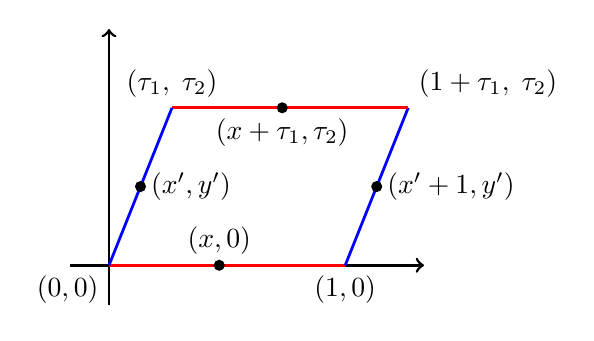
\begin{tikzpicture}[line width=1pt]
			
			% Parameters
			\def\L{3}          
			\def\tauone{0.8}   
			\def\tautwo{2.0}   
			
			% Axes
			\draw[->] (-0.5,0) -- (4,0);
			\draw[->] (0,-0.5) -- (0,3);
			
			% Parallelogram
			%\draw (0,0) -- (\L,0) -- ({\L+\tauone},{\tautwo}) -- (\tauone,\tautwo) -- cycle;
			% Define colors for horizontal and slanted lines
			\draw[red] (0,0) -- (\L,0);                           % Bottom (Horizontal)
			\draw[blue] (\L,0) -- ({\L+\tauone},{\tautwo});       % Right (Slanted)
			\draw[red] ({\L+\tauone},{\tautwo}) -- (\tauone,\tautwo); % Top (Horizontal)
			\draw[blue] (\tauone,\tautwo) -- (0,0);                % Left (Slanted)
			
			% Points and Labels for the Bottom-Top Identification
			\fill (\L/2-0.1, 0) circle (2pt);
			\node[above] at (\L/2-0.1, 0) {$ (x,0) $};
			
			\fill (\L/2-0.1+\tauone, \tautwo) circle (2pt);
			\node[below] at (\L/2-0.1+\tauone, \tautwo) {$ (x+\tau_{1}, \tau_{2}) $};
			
		% Points and Labels for the Left-Right Identification (z ~ z + L)
		\fill (\tauone/2, \tautwo/2) circle (2pt);
		\node[right] at (\tauone/2, \tautwo/2) {$ (x', y') $};
		
		\fill (\L+\tauone/2, \tautwo/2) circle (2pt);
		\node[right] at (\L+\tauone/2, \tautwo/2) {$ (x'+1, y') $};
			
			% Vertex labels
			\node[below left]  at (0,0) {$ (0,0) $};
			\node[below]       at (\L,0) {$ (1,0) $};
			\node[above]       at (\tauone,\tautwo) {$ (\tau_{1},\; \tau_{2}) $};
			\node[above right] at ({\L+\tauone},{\tautwo}) {$ (1+\tau_1,\; \tau_2) $};
			
		\end{tikzpicture}
	\end{minipage}	
	\hfill
	\begin{minipage}{0.45\textwidth}
	\begin{equation}
		\mathcolor{blue}{z \sim z + 1}, \quad \mathcolor{red}{z \sim z + \tau}.
	\end{equation}
	\end{minipage}
\end{center}

The original equation in the $w$-coordinate is:
\begin{equation}
	\frac{2}{\alpha'} \bar{\partial}_w \partial_w G'(w,w') = -2\pi \delta^{(2)}(w-w') + \frac{1}{2\pi\tau_2}.
\end{equation}
Under the coordinate transformation, we get $\bar{\partial}_w \partial_w = \frac{1}{4\pi^2} \bar{\partial}_z \partial_z$ and $\delta^{(2)}(w-w') = \frac{1}{4\pi^2} \delta^{(2)}(z)$, using which we obtain:
\begin{equation}
	\frac{2}{\alpha'} \bar{\partial}_z \partial_z G'(z) = -2\pi \delta^{(2)}(z) + \frac{\pi}{\tau_2}.
\end{equation}
The Laplacian is given by $\nabla_z^2 = 4 \bar{\partial}_z \partial_z$, through which the equation becomes:
\begin{equation}
	\nabla_z^2 G'(z) = 2\alpha' \left[ -2\pi \delta^{(2)}(z) + \frac{\pi}{\tau_2} \right].\label{green:torus}
\end{equation}
The eigenfunctions of $\nabla_z^2$ on the torus are plane waves $\Psi_{\vec{k}}(z) = \frac{1}{\sqrt{N}} e^{i\vec{k} \cdot \vec{z}}$, where the normalization constant $N$ is determined by the orthonormality condition:
\begin{equation}
	\int_{T^2} |\Psi_{\vec{k}}(z)|^2 d^2z = 1 \implies |N|^2 \int_{0}^{\tau_2} \int_{0}^{1} 2 \, dx \, dy = 1.
\end{equation}
Evaluating the integral gives $2\tau_2 |N|^2 = 1$, hence:
\begin{equation}
	N = \frac{1}{\sqrt{2\tau_2}}.
\end{equation}

The periodicities $z \sim z+1$ and $z \sim z+\tau$ restrict the momenta $\vec{k} = (k_x, k_y)$ to:
\begin{equation}
	k_x = 2\pi n, \quad k_y = \frac{2\pi(m - n\tau_1)}{\tau_2}, \quad n, m \in \mathbb{Z}.
\end{equation}
The eigenvalues of the Laplacian are given by:
\begin{equation}
	-|\vec{k}|^2 = -\left[ (2\pi n)^2 + \frac{4\pi^2(m - n\tau_1)^2}{\tau_2^2} \right] = -\frac{4\pi^2 |m - n\tau|^2}{\tau_2^2}.
\end{equation}
Having determined the eigenvalues, we expand $G'(z)$ and the source terms in the eigenfunction basis. The zero-mode of the source term vanishes:
\begin{equation}
	\int_{T^2} \left[ -2\pi \delta^{(2)}(z) + \frac{\pi}{\tau_2} \right]d^2z = -2\pi + \frac{\pi}{\tau_2}(2\tau_2) = 0.
\end{equation}
Therefore, we expand $G'(z) = \sum_{\vec{k} \neq 0} c_{n,m} e^{i\vec{k} \cdot \vec{z}}$ and $\delta^{(2)}(z)=\frac{1}{V_z}\sum_{\vec{k}=0}^{\infty}e^{i\vec{k}\cdot\vec{z}}$, and substitute into the differential equation \eqref{green:torus}:
\begin{equation}
	\sum_{\vec{k} \neq 0} -|\vec{k}|^2 c_{n,m} e^{i\vec{k} \cdot \vec{z}} = 2\alpha' \left( -\frac{2\pi}{N} \sum_{\vec{k} \neq 0} e^{i\vec{k} \cdot \vec{z}} \right).
\end{equation}
Solving for the coefficients $c_{n,m}$:
\begin{equation}
	c_{n,m} = \frac{4\pi \alpha'}{N |\vec{k}|^2} = \frac{4\pi \alpha'}{(2\tau_2) \left( \frac{4\pi^2 |m - n\tau|^2}{\tau_2^2} \right)} = \frac{\alpha' \tau_2}{2\pi |m - n\tau|^2}.
\end{equation}
Hence, the Green's function in the spectral representation is:
\begin{equation}
	G'(z) = \frac{\alpha' \tau_2}{2\pi} \sum_{(n,m) \neq (0,0)} \frac{1}{|m - n\tau|^2} \exp \left[ 2\pi i \left( nx + \frac{m - n\tau_1}{\tau_2}y \right) \right].
\end{equation}
The lattice sum can be evaluated using standard identities, yielding
\begin{equation}
\sum_{(n,m) \neq (0,0)} \frac{1}{|m - n\tau|^2} \exp \left[ 2\pi i \left( nx + \frac{m - n\tau_1}{\tau_2}y \right) \right] = -\frac{\pi}{\tau_2} \ln \left| \frac{\vartheta_1(z, \tau)}{\vartheta'_1(0|\tau)} \right|^2 + \frac{2\pi^2 y^2}{\tau_2^2} + k(\tau,\bar\tau).
\end{equation}
Upon substituting $z = \frac{w-w'}{2\pi}$ back into the equation, we obtain
\begin{align}
G'(w,w')&=-\frac{\alpha'}{2}\ln\left|\frac{\vartheta_1\!\left(\frac{w-w'}{2\pi}\Big|\tau\right)}{\vartheta_1'(0|\tau)}\right|^2+ \frac{\alpha'}{4\pi\tau_2}\,[\Im(w-w')]^2+ k(\tau,\bar\tau).
\end{align}
The constant $k(\tau,\bar\tau)$ is fixed by the orthogonality condition to the zero mode,
\begin{equation}
	\int_{T^2} d^2 w\, G'(w,w') = 0.
\end{equation}
QED.
\end{proof}
\end{tcolorbox}
Parallel to the previous result \eqref{6.2.13}, the expectation value of vertex operators is 
\begin{align}
	& \left\langle\prod_{i=1}^{n}: \mathrel{\me^{\mi k_{i} \cdot X(z_{i}, \bar{z}_{i})}}:\right\rangle \bigg._{\!\!T^{2}} 
	=\mi C_{T^{2}}^{X}(\tau)(2 \pi)^{d} \delta^{d}({\textstyle \sum_{i} k_{i}}) \nonumber \\
	&\qquad \qquad  \times \prod_{i<j}\left|\frac{2 \pi}{\partial_{\nu} \vartheta_{1}(0 \vert \tau)} 
	\vartheta_{1}\biggl(\frac{w_{i j}}{2 \pi} \Big\vert \tau\biggr) \exp 
	\biggl[-\frac{(\operatorname{Im} w_{i j})^{2}}{4 \pi \tau_{2}}\biggr]\right|^{\alpha^{\prime} k_{i} \cdot k_{j}} \:. \label{7.2.4} 
\end{align}
The factor $2 \pi / \partial_{\nu} \vartheta_{1}$ arises from renormalization of self-contractions. 

\subsection*{Scalar Partition Function} 
The total normalization for the sphere was absorbed into the string coupling constant, but we cannot do the same for the torus because it has a non-trivial $\tau$ dependence. 
In fact, we will see significant physics from amplitudes without vertex operators. 
Consider the path integral without vertex operators $\langle 1\rangle_{T^{2}(\tau)} \equiv Z(\tau) $. 
We can view the torus with modulus $\tau$ as a field theory on a circle evolving for Euclidean time $2 \pi \tau_{2}$, translated in the $\sigma^{1}$ direction by $2 \pi \tau_{1}$, and then identifying the ends. 
In the language of operators, this gives the trace 
\begin{align}
	Z(\tau) &=\operatorname{Tr}\Bigl[\exp (2 \pi \mi \tau_{1} P-2 \pi \tau_{2} H)\Bigr] \nonumber \\
	&=(q \bar{q})^{-d / 24} \operatorname{Tr}\Bigl(q^{L_{0}} \bar{q}^{\tilde{L}_{0}}\Bigr) \:. \label{7.2.5} 
\end{align}
Here $q=\exp (2 \pi \mi \tau)$. The momentum $P=L_{0}-\tilde{L}_{0}$ generates translations in $\sigma^{1}$, while the Hamiltonian $H=L_{0}+\tilde{L}_{0}-\frac{1}{24}(c+\tilde{c})$ generates translations in $\sigma^{2}$. 
As in statistical mechanics, this trace weighted by the exponential of the Hamiltonian and other conserved quantities is called the partition function. 

This trace can be split into a sum over occupation numbers $N_{\mu n}$ and $\tilde{N}_{\mu n}$ and an integral over momentum $k^{\mu}$. 
$Z(\tau)$ becomes 
\begin{equation}
	V_{d}(q \bar{q})^{-d / 24} \int \frac{\dif^{d} k}{(2 \pi)^{d}} \exp(-\pi \tau_{2} \alpha^{\prime} k^{2}) 
	\prod_{\mu, n} \sum_{N_{\mu n}, \tilde{N}_{\mu n}=0}^{\infty} q^{n N_{\mu n}} \bar{q}^{n \tilde{N}_{\mu n}} \:. \label{7.2.6} 
\end{equation}
The spacetime volume factor $V_{d}$ comes from the continuous normalization of momentum, where $\sum_{k}$ becomes $V_{d}(2 \pi)^{-d} \int \dif^{d} k$. 
The sum is a geometric series 
\begin{equation}
	\sum_{N=0}^{\infty} q^{n N}=(1-q^{n})^{-1} \:, \label{7.2.7} 
\end{equation}
yielding 
\begin{equation}
	Z(\tau)=\mi V_{d} Z_{X}(\tau)^{d} \:, \label{7.2.8} 
\end{equation}
where 
\begin{equation}
	Z_{X}(\tau)= (4 \pi^{2} \alpha^{\prime} \tau_{2})^{-1 / 2}|\eta(\tau)|^{-2} \:. \label{7.2.9} 
\end{equation}
Here 
\begin{equation}
	\eta(\tau)=q^{1 / 24} \prod_{n=1}^{\infty}(1-q^{n}) \label{7.2.10} 
\end{equation}
is the Dedekind eta function. The factor of $\mi$ comes from the rotation $k^{0} \rightarrow \mi k^{d}$. Also, previously $C_{T^{2}}^{X}(\tau)=Z_{X}(\tau)^{d}$. 

\eqref{7.2.8} is clearly invariant under $\tau \rightarrow \tau+1$. 
The invariance of $Z_{X}$ under $\tau \rightarrow-1 / \tau$ is given by \eqref{7.2.44}, $\eta(-1 / \tau)=(-\mi \tau)^{1 / 2} \eta(\tau)$. 
This generates the entire modular group. Similarly, expectation values with vertex operators are modular covariant. 

This calculation can be performed using holomorphy. The main idea is to obtain a differential equation for $\tau$. 
Consider a torus with modulus $\tau$ and make a small change to the metric $\delta g_{w w}=\epsilon^{*}$. 
The new metric is 
\begin{align}
	\dif s^{2} &= \dif w \dif \bar{w}+\epsilon^{*} \dif w^{2}+\epsilon \dif \bar{w}^{2}  \nonumber \\
	&=(1+\epsilon^{*}+\epsilon) \dif[w+\epsilon(\bar{w}-w)]\, \dif[\bar{w}+\epsilon^{*}(w-\bar{w})]+O(\epsilon^{2}) \:. \label{7.2.11} 
\end{align}
That is, this metric is Weyl equivalent to $\dif w^{\prime} \dif \bar{w}^{\prime}$, where $w^{\prime}=w+\epsilon(\bar{w}-w)$. It has periodicity 
\begin{equation}
	w^{\prime} \cong w^{\prime}+2 \pi \cong w^{\prime}+2 \pi(\tau-2 \mi \tau_{2} \epsilon) \:. \label{7.2.12} 
\end{equation}
The change in the metric is thus equivalent to a change in the modulus 
\begin{equation}
	\delta \tau=-2 \mi \tau_{2} \epsilon \:. \label{7.2.13} 
\end{equation}

After changing the metric, the change in the path integral is 
\begin{align}
	\delta Z(\tau) &= -\frac{1}{2 \pi} \int \dif^{2} w \: \Bigl[\delta g_{\bar{w} \bar{w}} 
	\bigl\langle T_{w w}(w)\bigr\rangle+\delta g_{w w}\bigl\langle T_{\bar{w} \bar{w}}(\bar{w})\bigr\rangle\Bigr] \nonumber \\
	&=-2 \pi \mi\Bigl[\delta \tau \bigl\langle T_{w w}(0)\bigr\rangle - \delta \bar{\tau}\bigl\langle T_{\bar{w} \bar{w}}(0)\bigr\rangle\Bigr] \:. \label{7.2.14} 
\end{align}
In the second line, we used translation invariance to perform the integration. To find the expectation value of the energy-momentum tensor, we use the OPE 
\begin{equation}
	\partial_{w} X^{\mu}(w) \partial_{w} X_{\mu}(0)=-\frac{\alpha^{\prime} d}{2 w^{2}}-\alpha^{\prime} T_{w w}(0)+O(w^{2}) \:. \label{7.2.15} 
\end{equation}
Now, 
\begin{align}
	Z(\tau)^{-1}\langle\partial_{w} X^{\mu}(w) \partial_{w} X_{\mu}(0)\rangle 
	&= \partial_{w} \partial_{w^{\prime}} G^{\prime}(w, \bar{w} ; w^{\prime}, \bar{w}^{\prime})|_{w^{\prime}=0} \nonumber \\
	&=\frac{\alpha^{\prime} d}{2} \frac{\vartheta_{1} \partial_{w}^{2} \vartheta_{1}-\partial_{w} \vartheta_{1} \partial_{w} \vartheta_{1}}{\vartheta_{1}^{2}}+\frac{\alpha^{\prime} d}{8 \pi \tau_{2}} \:, \label{7.2.16} 
\end{align}
where all variables of the theta functions are $(w / 2 \pi, \tau)$. 
It indeed has a double pole at $w=0 $. Carefully expanding the numerator and denominator to order $w^{2}$, the $w^{0}$ term in \eqref{7.2.16} is 
\begin{equation}
	\frac{\alpha^{\prime} d}{6} \frac{\partial_{w}^{3} \vartheta_{1}}{\partial_{w} \vartheta_{1}}+\frac{\alpha^{\prime} d}{8 \pi \tau_{2}} \:. \label{7.2.17} 
\end{equation}
Then the OPE \eqref{7.2.15} gives 
\begin{equation}
	\langle T_{w w}(0)\rangle=\left(-\frac{d}{6} \frac{\partial_{w}^{3} \vartheta_{1}(0 \vert \tau)}{\partial_{w} \vartheta_{1}(0 \vert\tau)}-\frac{d}{8 \pi \tau_{2}}\right) Z(\tau) \:, \label{7.2.18} 
\end{equation}
and the variation \eqref{7.2.14} gives the differential equation 
\begin{equation}
	\partial_{\tau} \ln Z(\tau)=\frac{\pi \mi d}{3} \frac{\partial_{w}^{3} \vartheta_{1}(0 \vert \tau)}{\partial_{w} \vartheta_{1}(0 \vert \tau)}+\frac{\mi d}{4 \tau_{2}} \:. \label{7.2.19} 
\end{equation}
To go further, using 
\begin{equation}
	\partial_{w}^{2} \vartheta_{1}\biggl(\frac{w}{2 \pi} \Big\vert \tau\biggr) = 
	\frac{\mi}{\pi} \partial_{\tau} \vartheta_{1}\biggl(\frac{w}{2 \pi} \Big\vert \tau \biggr) \:. \label{7.2.20} 
\end{equation}
Rewrite \eqref{7.2.19} as 
\begin{equation}
	\partial_{\tau} \ln Z(\tau)=-\frac{d}{3} \partial_{\tau} \ln \partial_{w} \vartheta_{1}(0 \vert \tau)+\frac{\mi d}{4 \tau_{2}} \:. \label{7.2.21} 
\end{equation}
Together with the conjugate equation, this determines $Z(\tau)$ up to a numerical coefficient as 
\begin{equation}
	Z(\tau)=|\partial_{w} \vartheta_{1}(0 \vert \tau)|^{-2 d / 3} \tau_{2}^{-d / 2} \:, \label{7.2.22} 
\end{equation}
The numerical coefficient is determined by other methods. Using \eqref{7.2.43}, we can see it matches \eqref{7.2.8}. 

\subsection*{$bc$ CFT} 

For the ghost CFT, the partition function is also determined by the trace of states. 
On both the left and right sides, there are two sets of creation operators $b_{-n}$ and $c_{-n}$, but they are anticommutative. Thus, occupation numbers can only be 0 or 1. 
Therefore, an oscillator of mode $n$ contributes $(1+q^{n})$. Additionally, there are four ground states, which give 
\begin{align}
	\operatorname{Tr}\Bigl[\exp (2 \pi \mi \tau_{1} P-2 \pi \tau_{2} H)\Bigr] &= 
	(q \bar{q})^{13 / 12} \operatorname{Tr}\Bigl(q^{L_{0}} \bar{q}^{\tilde{L}_{0}}\Bigr) \nonumber \\
	&=4(q \bar{q})^{1 / 12} \prod_{n=1}^{\infty}|1+q^{n}|^{4} \:. \label{7.2.23} 
\end{align}

However, for anticommutative fields, this trace corresponds to a path integral with anti-periodic boundaries in the time direction. To calculate the Faddeev-Popov determinant, the ghost fields must have the same periodicity as the original coordinate transformation, which is periodic. 
Therefore, we need 
\begin{align}
	Z(\tau) &=\operatorname{Tr}\Bigl[(-1)^{F} \exp (2 \pi \mi \tau_{1} P-2 \pi \tau_{2} H)\Bigr] \nonumber \\
	&=0 \:, \label{7.2.24} 
\end{align}
where $(-1)^{F}$ anticommutes with all ghost fields. 
The trace is zero because the ghost numbers of $\lvert \downarrow \downarrow\rangle$ and $\lvert\uparrow \uparrow\rangle$ are opposite to those of $\lvert \uparrow \downarrow\rangle$ and $\lvert\downarrow \uparrow\rangle$ modulo 2. 
From the path integral viewpoint, $Z(\tau)$ is zero due to ghost zero modes arising from the moduli and CKVs. 
They must be saturated by suitable insertions. The simplest non-zero amplitude is 
\begin{equation}
	\Bigl\langle c(w_{1}) b(w_{2}) \tilde{c}(\bar{w}_{3}) \tilde{b}(\bar{w}_{4})\Bigr\rangle \:. \label{7.2.25} 
\end{equation}
In the operator calculation, we write each field in its mode expansion. Only the $n=0$ terms contribute. 
Then \eqref{7.2.25} becomes 
\begin{equation}
	\operatorname{Tr}\Bigl[(-1)^{F} c_{0} b_{0} \tilde{c}_{0} \tilde{b}_{0} \exp (2 \pi \mi \tau_{1} P-2 \pi \tau_{2} H)\Bigr] \:. \label{7.2.26} 
\end{equation}
The operator $c_{0} b_{0} \tilde{c}_{0} \tilde{b}_{0}$ projects onto the ground state $\lvert\uparrow \uparrow\rangle$, so the result is 
\begin{equation}
	(q \bar{q})^{1 / 12} \prod_{n=1}^{\infty}|1-q^{n}|^{4}=|\eta(\tau)|^{4} \:. \label{7.2.27} 
\end{equation}
Note the sign change in the infinite product comes from $(-1)^{F}$ in the trace. Since the CKVs and quadratic differentials on the torus are constant, \eqref{7.2.27} is independent of the position of the ghost fields. 

\subsection*{General CFT} 
For a general CFT % 
\begin{equation}
	Z(\tau)=\sum_{i} q^{h_{i}-c / 24} \bar{q}^{\tilde{h}_{i}-\tilde{c} / 24}(-1)^{F_{i}} \:, \label{7.2.28} % 
\end{equation}
where $i$ runs over all states of the CFT, and $F_{i}$ is the worldsheet fermion number. Invariance under $\tau \rightarrow \tau+1$ requires $h_{i}-\tilde{h}_{i}-\frac{1}{24}(c-\tilde{c})$ to be an integer. % 
Considering the identity operator, this requires $c-\tilde{c}$ to be a multiple of 24. For general operators, this then requires integer spin % 
\begin{equation}
	h_{i}-\tilde{h}_{i} \in \mathds{Z} \:. \label{7.2.29} % 
\end{equation}
Incidentally, CFTs where $c-\tilde{c}$ is not a multiple of 24 must also be interesting. They cannot be modular invariant alone, but with suitable projections, they can be integrated into a modular invariant theory. % 

Invariance under $\tau \rightarrow-1 / \tau$ imposes further restrictions on the spectrum. 
Consider the partition function with $\tau=\mi \ell$, and let $\ell \rightarrow 0 $; the convergence factor $q=\exp (-2 \pi \ell)$ approaches 1. 
Thus, the partition function is determined by the density of the highest weight states. 
Using modular invariance, this equals the partition function with $\tau=\mi / \ell $, where the latter's $q=\exp (-2 \pi / \ell)$ approaches 0. 
Thus, the lowest weight state dominates the sum, which is the identity state with $L_{0}=\tilde{L}_{0}=0$, yielding 
\begin{equation}
	Z(\mi \ell) \stackrel{l \rightarrow 0}{\approx} \exp \left[\frac{\pi(c+\tilde{c})}{12 \ell}\right] \:. \label{7.2.30} 
\end{equation}
The density of highest weight states is thus determined by the central charge. This produces the result for free bosons, where $c=\tilde{c}=d$ counts the number of free bosons. 

\subsection*{Theta Functions} 
The fundamental theta function is 
\begin{equation}
	\vartheta(\nu, \tau)=\sum_{n=-\infty}^{\infty} \exp (\pi \mi n^{2} \tau+2 \pi \mi n \nu) \:. \label{7.2.31} 
\end{equation}
It has periodicities 
\begin{subequations}  \label{7.2.32}
	\begin{align}
		\vartheta(\nu+1, \tau) &= \vartheta(\nu, \tau) \:, \label{7.2.32a}  \\
		\vartheta(\nu+\tau, \tau) &= \exp (-\pi \mi \tau-2 \pi \mi \nu) \vartheta(\nu, \tau) \:, \label{7.2.32b} 
	\end{align}
\end{subequations}
and under modular transformations 
\begin{subequations} \label{7.2.33}
	\begin{align}
		\vartheta(\nu, \tau+1) &= \vartheta(\nu + 1/2, \tau) \:, \label{7.2.33a} \\
		\vartheta(\nu/\tau, -1/\tau) &=(-\mi \tau)^{1 / 2} \exp (\pi \mi \nu^{2} / \tau) \vartheta(\nu, \tau) \:. \label{7.2.33b} 
	\end{align}
\end{subequations}
Aside from the periodicity \eqref{7.2.32}, the theta function has only one zero at $v=\frac{1}{2}(1+\tau)$. It can also be written as an infinite product 
\begin{equation}
	\vartheta(\nu, \tau)=\prod_{m=1}^{\infty}(1-q^{m})(1+z q^{m-1 / 2})(1+z^{-1} q^{m-1 / 2}) \:, \label{7.2.34} 
\end{equation}
where 
\begin{equation}
	q=\exp (2 \pi \mi \tau), \quad z=\exp (2 \pi \mi\nu) \:. \label{7.2.35} 
\end{equation}

We often need the asymptotic behavior of theta functions as $q \rightarrow 0$ or $q \rightarrow 1$. $q \rightarrow 0$ can be read immediately from the product or sum. The behavior at $q \rightarrow 1$ is less obvious but can be obtained from the modular transformation $\tau \rightarrow-1 / \tau$, which relates the two limits via $q \rightarrow \exp \left(4 \pi^{2} / \ln q\right)$. 
It is often useful to define theta functions with characteristics 
\begin{align}
	\vartheta\bigl[\!\begin{smallmatrix} a\\b\end{smallmatrix}\!\bigr]
	(\nu, \tau) &=\exp \Bigl[\pi \mi a^{2} \tau+2 \pi \mi a(\nu+b)\Bigr] \vartheta(\nu+a \tau+b, \tau)  \nonumber \\
	&=\sum_{n=-\infty}^{\infty} \exp \Bigl[\pi \mi(n+a)^{2} \tau+2 \pi \mi(n+a)(\nu+b)\Bigr] \:. \label{7.2.36} 
\end{align}
Other common notations are 
\begin{subequations} \label{7.2.37}
	\begin{align}
		\vartheta_{00}(\nu, \tau)&=\vartheta_{3}(\nu \vert \tau)= 
		\vartheta\bigl[\!\begin{smallmatrix} 0\\0\end{smallmatrix}\!\bigr](\nu, \tau) = \sum_{n=-\infty}^{\infty} q^{n^{2} / 2} z^{n} \:, 
		\label{7.2.37a}  \\
		\vartheta_{01}(\nu, \tau) &= \vartheta_{4}(\nu \vert \tau)=
		\vartheta\bigl[\!\begin{smallmatrix} 0\\1/2\end{smallmatrix}\!\bigr](\nu, \tau)=
		\sum_{n=-\infty}^{\infty}(-1)^{n} q^{n^{2} / 2} z^{n} \:, \label{7.2.37b}\\
		\vartheta_{10}(\nu, \tau) &= \vartheta_{2}(\nu \vert \tau) = 
		\vartheta\bigl[\!\begin{smallmatrix} 1/2\\0\end{smallmatrix}\!\bigr](\nu, \tau)
		=\sum_{n=-\infty}^{\infty} q^{(n-1 / 2)^{2} / 2} z^{n-1 / 2}  \:, \label{7.2.37c} \\
		\vartheta_{11}(\nu, \tau)&=-\vartheta_{1}(\nu \vert \tau) = 
		\vartheta\bigl[\!\begin{smallmatrix} 1/2\\1/2\end{smallmatrix}\!\bigr](\nu, \tau)
		=-\mi \sum_{n=-\infty}^{\infty}(-1)^{n} q^{(n-1 / 2)^{2} / 2} z^{n-1 / 2} \:. \label{7.2.37d} 
	\end{align}
\end{subequations}
Product representations: 
\begin{subequations} \label{7.2.38}
	\begin{align}
		\vartheta_{00}(\nu, \tau) &= \prod_{m=1}^{\infty}(1-q^{m})(1+z q^{m-1/2})(1+z^{-1} q^{m-1/2}) \:, \label{7.2.38a} \\ 
		\vartheta_{01}(\nu, \tau) &= \prod_{m=1}^{\infty}(1-q^{m})(1-z q^{m-1/2})(1-z^{-1} q^{m-1/2}) \:, \label{7.2.38b} \\
		\vartheta_{10}(\nu, \tau) &= 2 \exp (\pi \mi \tau / 4) \cos \pi \nu 
		\prod_{m=1}^{\infty}(1-q^{m})(1+z q^{m})(1+z^{-1} q^{m}) \:, \label{7.2.38c} \\
		\vartheta_{11}(\nu, \tau) &= -2 \exp (\pi \mi \tau / 4) \sin \pi \nu 
		\prod_{m=1}^{\infty}(1-q^{m})(1-z q^{m})(1-z^{-1} q^{m})  \:. \label{7.2.38d} 
	\end{align}	
\end{subequations}
Modular transformations 
\begin{subequations} \label{7.2.39}
	\begin{align}
		\vartheta_{00}(\nu, \tau+1) &= \vartheta_{01}(\nu, \tau)  \:, \label{7.2.39a} \\
		\vartheta_{01}(\nu, \tau+1) &= \vartheta_{00}(\nu, \tau)  \:, \label{7.2.39b} \\
		\vartheta_{10}(\nu, \tau+1) &= \exp (\pi \mi / 4) \vartheta_{10}(\nu, \tau) \:, \label{7.2.39c} \\
		\vartheta_{11}(\nu, \tau+1) &= \exp (\pi \mi / 4) \vartheta_{11}(\nu, \tau) \:, \label{7.2.39d}
	\end{align}
\end{subequations}
and 
\begin{subequations} \label{7.2.40}
	\begin{align}
		\vartheta_{00}(\nu/\tau,-1 / \tau) &= (-\mi \tau)^{1/2} \exp(\pi \mi \nu^{2}/\tau) \vartheta_{00}(\nu, \tau) \:, \label{7.2.40a} \\
		\vartheta_{01}(\nu/\tau,-1 / \tau) &= (-\mi \tau)^{1/2} \exp(\pi \mi \nu^{2}/\tau) \vartheta_{10}(\nu, \tau) \:, \label{7.2.40b} \\
		\vartheta_{10}(\nu/\tau,-1 / \tau) &= (-\mi \tau)^{1/2} \exp(\pi \mi \nu^{2}/\tau) \vartheta_{01}(\nu, \tau) \:, \label{7.2.40c} \\
		\vartheta_{11}(\nu/\tau,-1 / \tau) &=-\mi(-\mi \tau)^{1/2} \exp(\pi \mi \nu^{2}/\tau) \vartheta_{11}(\nu, \tau) \:. \label{7.2.40d} 
	\end{align}
\end{subequations}
We will encounter these functions more frequently in superstrings. 

Theta functions satisfy Jacobi's ``abstruse identity'', which is a special case of the Riemann quartic identity 
\begin{equation}
	\vartheta_{00}^{4}(0, \tau)-\vartheta_{01}^{4}(0, \tau)-\vartheta_{10}^{4}(0, \tau)=0 \:. \label{7.2.41}
\end{equation}
Also note 
\begin{equation}
	\vartheta_{11}(0, \tau)=0 \:. \label{7.2.42} 
\end{equation}
Finally, the Dedekind eta function is 
\begin{equation}
	\eta(\tau)=q^{1 / 24} \prod_{m=1}^{\infty}(1-q^{m})=\left[\frac{\partial_{\nu} \vartheta_{11}(0, \tau)}{-2 \pi}\right]^{1/3} \:. \label{7.2.43} 
\end{equation}
Modular transformations 
\begin{subequations} \label{7.2.44}
	\begin{align}
		\eta(\tau+1) &=\exp (\mi \pi / 12) \eta(\tau)  \:, \label{7.2.44a} \\
		\eta(-1 / \tau) &=(-\mi \tau)^{1 / 2} \eta(\tau) \:. \label{7.2.44b} 
	\end{align}
\end{subequations}

\section{\texorpdfstring{Torus Amplitudes}{7.3 Torus Amplitudes}} \label{sec:7.3} 
We now apply the general result \eqref{5.3.9} to the torus: expressing string scattering amplitudes as integrals with ghost and vertex operator insertions. Two CKVs require one vertex operator to be fixed, so 
\begin{align}
	&S_{T^{2}}(1 ; 2 ; \ldots ; n)  \nonumber \\
	&\quad=\frac{1}{2} \int_{F_{0}} \dif \tau \dif \bar{\tau} \:
	\biggl\langle B \tilde{B} \tilde{c} c \mathscr{V}_{1}(w_{1}, \bar{w}_{1}) 
	\prod_{i=2}^{n} \int \dif w_{i} \dif \bar{w}_{i} \: \mathscr{V}_{i}(w_{i}, \bar{w}_{i})\biggr\rangle_{T^{2}} \:. \label{7.3.1} 
\end{align}
The fundamental region $F_{0}$ is the same as discussed in section \ref{sec:5.1}, and the $\frac{1}{2}$ comes from $w \rightarrow-w$. As with complex field variables, $\dif \tau \dif \bar{\tau}=2 \dif \tau_{1} \dif \tau_{2}$, where $\tau=\tau_{1}+\mi \tau_{2}$. 
The ghost insertion for $\dif \tau$ is 
\begin{align}
	B=\frac{1}{4 \pi}(b, \partial_{\tau}) &=\frac{1}{2 \pi} \int \dif^{2} w \: b_{w w}(w) \partial_{\tau} g_{\bar{w} \bar{w}} \nonumber \\
	&=\frac{\mi}{4 \pi \tau_{2}} \int \dif^{2} w \: b_{w w}(w) \nonumber \\
	& \rightarrow 2 \pi \mi b_{w w}(0) \:. \label{7.3.2} 
\end{align}
We used \eqref{7.2.13}. In the last line, we used the fact that the ghost path integral \eqref{7.2.27} is position-independent. 

The CKG is composed of translations of the torus. Since this group has a finite volume, we do not need to fix it; we can rewrite the amplitude to integrate over all vertex operators and then divide by the volume of the CKG. CKVs are constant, so the expectation value in \eqref{7.3.1} is independent of the position of $c$: we can move $c$ away from $w_{1}$ and place them at some fixed location. For vertex operators, translation invariance implies the amplitude is invariant under $w_{i} \rightarrow w_{i}+w$. 
Average over this translation: 
\begin{equation}
	\int \frac{\dif w \dif \bar{w}}{2(2 \pi)^{2} \tau_{2}} \:, \label{7.3.3} 
\end{equation}
where the denominator is the area of the torus, which is the volume of the CKG. 
Using \eqref{7.3.2} and \eqref{7.3.3}, the amplitude becomes 
\begin{align}
	&S_{T^{2}}(1 ; 2 ; \ldots ; n) \nonumber \\
	&\quad=\int_{F_{0}} \frac{\dif \tau \dif \bar{\tau}}{4 \tau_{2}} 
	\biggl\langle b(0) \tilde{b}(0) \tilde{c}(0) c(0) \prod_{i=1}^{n} \int \dif w_{i} \dif \bar{w}_{i}\: 
	\mathscr{V}_{i}(w_{i}, \bar{w}_{i})\biggr\rangle_{T^{2}} \:. \label{7.3.4} 
\end{align}
Now all vertex operators have equal status. 
\begin{tcolorbox}
	\begin{remark}
		The factor $(4\tau_{2})^{-1}$ in \eqref{7.3.4} comes from $1/2$ in \eqref{7.3.1}, $(2\pi)^{-2}$ in \eqref{7.3.2}, and $(2(2\pi )^2 \tau _2 )^{-1}$ in \eqref{7.3.3}.
	\end{remark}
\end{tcolorbox}

Without the intermediate step of fixing vertex operators, \eqref{7.3.4} can also be derived directly; even without vertex operators, it holds: 
\begin{equation}
	Z_{T^{2}}=\int_{F_{0}} \frac{\dif \tau \dif \bar{\tau}}{4 \tau_{2}} \:
	\Bigl\langle b(0) \tilde{b}(0) \tilde{c}(0) c(0)\Bigr\rangle_{T^{2}} \:. \label{7.3.5} 
\end{equation}
This vacuum amplitude is quite interesting and will be our main goal of study. It not only reveals that the UV behavior of string theory differs from field theory, but also has significant physical meaning itself. 

For 26 flat spacetime dimensions, the path integrals of matter and ghost fields in \eqref{7.3.5} were calculated in the previous section, yielding 
\begin{equation}
	Z_{T^{2}}=\mi V_{26} \int_{F_{0}} \frac{\dif \tau \dif \bar{\tau}}{4 \tau_{2}} \: 
	(4 \pi^{2} \alpha^{\prime} \tau_{2})^{-13}|\eta(\tau)|^{-48} \:. \label{7.3.6} 
\end{equation}
This amplitude has an important property: modular invariance. According to \eqref{7.2.44}, $\tau_{2}|\eta(\tau)|^{4}$ is modular invariant, and it is easy to verify that 
\begin{equation}
	\frac{\dif \tau \dif \bar{\tau}}{\tau_{2}^{2}} \label{7.3.7} 
\end{equation}
is also modular invariant. Note that the exponent $-48$ comes from 24 sets of left-moving and 24 sets of right-moving oscillators. Ghost contributions cancel two sets of oscillators, leaving only the transverse mode contributions. By introducing vertex operators into the expectation value \eqref{7.2.4} and integrating over position, we get the $n$-tachyon amplitude. 
\begin{tcolorbox}
	\begin{itemize}
		\item 
		According to \eqref{7.2.9}, $[Z_{X}(\tau)]^{26}=(4 \pi^{2} \alpha^{\prime} \tau_{2})^{-13}|\eta(\tau)|^{-52}$, and according to \eqref{7.2.27}, $\langle c b \tilde{c} \tilde{b}\rangle=|\eta(\tau)|^{4}$. Multiplying them gives \eqref{7.3.6}. 
		\item Regarding modular invariance, the invariance under $\tau\to\tau+1$ is trivial. Under $\tau\to -1/\tau$, we have $\tau_{2}\to \tau_{2}/|\tau|^{2}$ and $\dif \tau \to (-\tau^{-2})\dif\tau$, which gives the modular invariance of \eqref{7.3.7}. 
	\end{itemize}
\end{tcolorbox}

For a general CFT, the path integral on the torus is expressed by the trace in \eqref{7.2.28}. 
As long as there are $d \geq 2$ non-compact flat dimensions, the ghost fields still cancel two sets of bosonic operators, and the vacuum amplitude is 
\begin{subequations} \label{7.3.8}
	\begin{align}
		Z_{T^{2}} &=V_{d} \int_{F_{0}} \frac{\dif \tau \dif \bar{\tau}}{4 \tau_{2}} \int \frac{\dif^{d} k}{(2 \pi)^{d}}\: 
		\exp (-\pi \tau_{2} \alpha^{\prime} k^{2}) \sum_{i \in \mathscr{H}^{\perp}} q^{h_{i}-1} \bar{q}^{\tilde{h}_{i}-1} \label{7.3.8a}  \\
		&= \mi V_{d} \int_{F_{0}} \frac{\dif \tau \dif \bar{\tau}}{4 \tau_{2}} \: (4 \pi^{2} \alpha^{\prime} \tau_{2})^{-d / 2} 
		\sum_{i \in \mathscr{H}^{\perp}} q^{h_{i}-1} \bar{q}^{\tilde{h}_{i}-1}  \label{7.3.8b}
	\end{align}		
\end{subequations}
Here $\mathscr{H}^{\perp}$ is the closed string Hilbert space excluding ghosts, $\mu=0,1$ oscillators, and non-compact momentum. 
To understand the physics of these amplitudes, it is useful to compare them with the corresponding quantities in field theory, summing over all paths with circle topology. This is given by 
\begin{align}
	Z_{S_{1}}(m^{2}) &=V_{d} \int \frac{\dif^{d} k}{(2 \pi)^{d}} \int_{0}^{\infty} \frac{\dif l}{2 l}  \: 
	\exp [-(k^{2}+m^{2}) l / 2] \nonumber \\
	&=\mi V_{d} \int_{0}^{\infty} \frac{\dif l}{2 l}(2 \pi l)^{-d / 2} \: \exp (-m^{2} l / 2)   \label{7.3.9} 
\end{align}
This can be derived through gauge-fixed point-particle path integrals. The result is intuitive: $l$ is the modulus of the circle, $\frac{1}{2}(k^{2}+m^{2})$ is the Hamiltonian of the worldline, and $2 l$ removes redundant counting from translations and reversing worldline coordinates. 

We now adopt the point-particle result for particles of mass $m^{2}$ and sum over the string spectrum. As stated in Chapter \ref{cha:4}, the physical spectrum corresponds one-to-one with $\mathscr{H}^{\perp}$, where the relationship between mass and transverse weight is 
\begin{equation}
	m^{2}=\frac{2}{\alpha^{\prime}}(h+\tilde{h}-2) \label{7.3.10} 
\end{equation}
subject to the constraint $h=\tilde{h}$. 
This constraint can be written in integral form 
\begin{equation}
	\delta_{h, \tilde{h}}=\int_{-\pi}^{\pi} \frac{\dif \theta}{2 \pi} \exp \Bigl[\mi(h-\tilde{h}) \theta\Bigr] \:. \label{7.3.11} 
\end{equation}
In the above, we assume $h-\tilde{h}$ is an integer. This is true in 26 flat dimensions; as discussed in the previous section, modular invariance is generally important. 
Then 
\begin{align}
	\sum_{i \in \mathscr{H} \perp} Z_{S_{1}}(m_{i}^{2}) &= \mi V_{d} \int_{0}^{\infty} \frac{\dif l}{2 l} 
	\int_{-\pi}^{\pi} \frac{\dif \theta}{2 \pi} \: (2 \pi l)^{-d / 2} \nonumber \\
	&\qquad \qquad  \times \sum_{i \in \mathscr{H}^{\perp}} \exp \Bigl[-(h_{i}+\tilde{h}_{i}-2) l / \alpha^{\prime}
	+\mi(h_{i}-\tilde{h}_{i}) \theta\Bigr]  \nonumber \\
	&=\mi V_{d} \int_{R} \frac{\dif \tau \dif \bar{\tau}}{4 \tau_{2}}\: (4 \pi^{2} \alpha^{\prime} \tau_{2})^{-d / 2} 
	\sum_{i \in \mathscr{H} \perp} q^{h_{i}-1} \bar{q}^{\tilde{h}_{i}-1} \:, \label{7.3.12} 
\end{align}
where $\theta+\mi l / \alpha^{\prime}=2 \pi \tau$. 
Integration region $R$: 
\begin{equation}
	R: \quad \tau_{2}>0, \quad |\tau_{1}|<\frac{1}{2} \:. \label{7.3.13} 
\end{equation}

We now interpret this result. A single point-particle amplitude \eqref{7.3.9} diverges as $l \rightarrow 0$. This is the standard UV divergence of quantum field theory. Summing over the string spectrum as in \eqref{7.3.12} only worsens the situation, as all string contributions have the same sign. However, comparing \eqref{7.3.12} with the actual string amplitude \eqref{7.3.8}, they are very similar with one significant difference. 
The integration regions differ: in string theory, it is the fundamental domain 
\begin{equation}
	F_{0}: \quad|\tau|>1, \quad |\tau_{1}|<\frac{1}{2}, \quad \tau_{2}>0 \label{7.3.14} 
\end{equation}
The UV divergence region is bypassed. We can also see this from the momentum integral \eqref{7.3.8a}. 

Another possible divergence comes from the limit $\tau_{2} \rightarrow \infty$, when the torus becomes very long. 
In this region, the string amplitude in 26 dimensions has the expansion 
\begin{equation}
	\mi V_{26} \int^{\infty} \frac{\dif \tau_{2}}{2 \tau_{2}} \:(4 \pi^{2} \alpha^{\prime} \tau_{2})^{-13}
	\Bigl[\exp (4 \pi \tau_{2})+24^{2}+\cdots\Bigr] \:, \label{7.3.15} 
\end{equation}
The asymptotic behavior is controlled by the lightest string states. The first term in the series diverges, and from the field theory perspective, the explanation is obvious: the series is arranged in order of increasing mass squared. 
The first term comes from the tachyon, and the divergence arises from the positive exponent in the path sum \eqref{7.3.9}. This is a product of a theory containing tachyons and does not affect more realistic theories. Incidentally, this path sum can be defined by analytic continuation of positive mass squared, but problems remain—the continued energy density is complex. This signifies instability, where the tachyon field rolls down its inverted potential. For general CFT, \eqref{7.3.12} becomes 
\begin{equation}
	\mi V_{d} \int^{\infty} \frac{\dif \tau_{2}}{2 \tau_{2}} \: (4 \pi^{2} \alpha^{\prime} \tau_{2})^{-d / 2} 
	\sum_{i} \exp (-\pi \alpha^{\prime} m_{i}^{2} \tau_{2}) \:. \label{7.3.16} 
\end{equation}
Since tachyons always appear in bosonic string theory, this is divergent; without tachyons, it would be convergent. 

The torus exemplifies a general principle that holds for all string amplitudes: there is no UV region in moduli space giving rise to high-energy divergences. All limits are controlled by the lightest string states, i.e., long-range physics. For the torus with vertex operators, the $\tau$ integral is still truncated as above. But more limits exist when vertex operators approach each other. The same general principle applies to them, which we will discuss further in Chapter \ref{cha:9}. 

By truncating the $l$ integral, we can attempt to remove UV divergences in field theory. 
Similarly, one can try to make similar corrections to string theory. For example, replacing the usual fundamental domain $F_{0}$ with $|\tau_{1}| \leq \frac{1}{2}$, $\tau_{2}>1$. 
However, in either case, this would destroy the consistency of the theory: non-physical negative-norm states will no longer decouple. We saw in the general discussion of section \ref{sec:5.4} that the coupling of BRST-null states is proportional to the total derivative on moduli space. 
For the fundamental domain $F_{0}$, the boundaries I and $\mathrm{I}^{\prime}$, and II and $\mathrm{II}^{\prime}$ are equivalent, so boundary terms cancel. Modifying the integration region would introduce real boundaries, and surface terms on moduli space would no longer cancel. Thus, there would be non-zero amplitudes for null states and an inconsistent quantum theory. If we make a brute-force truncation to make a gravity theory finite, this is a direct analogy of the consequence: it is extremely difficult to do so without destroying local spacetime symmetry and making the theory inconsistent. 
String theory provides a subtle way that softens short-distance behavior and eliminates divergences without losing spacetime gauge invariance. 

\subsection*{Physics of the Vacuum Amplitude} 
Besides exemplifying the behavior of string amplitudes, the one-loop vacuum amplitude has an interesting physical interpretation. In point-particle theory, "vacuum" paths consist of any $n$ non-intersecting circles. Permutation symmetry introduces a factor $1/n!$, and summing over $n$ gives 
\begin{equation}
	\bm{Z}_{\mathrm{vac}}(m^{2})=\exp \Bigl[Z_{S_{1}}(m^{2})\Bigr] \:. \label{7.3.17} 
\end{equation}
Switching to canonical field theory, 
\begin{align}
	Z_{\mathrm{vac}}(m^{2}) &= \langle 0|\exp (-\mi H T)| 0\rangle \nonumber \\
	&=\exp (-\mi \rho_{0} V_{d}) \:, \label{7.3.18} 
\end{align}
where $\rho_{0}$ is the vacuum energy density: 
\begin{equation}
	\rho_{0}=\frac{\mi}{V_{d}} Z_{S_{1}}(m^{2}) \:. \label{7.3.19} 
\end{equation}

The $l$ integral in $Z_{S_{1}}(m^{2})$ diverges as $l \rightarrow 0 $. In renormalizable field theory, this is cancelled by counterterms or supersymmetry. 
We truncate the integral $l \geq \epsilon$ and then take $\epsilon \rightarrow 0$, but discard the divergent terms. Under this treatment, 
\begin{equation}
	\int_{0}^{\infty} \frac{\dif l}{2 l} \exp [-(k^{2}+m^{2}) l / 2] \rightarrow-\frac{1}{2} \ln(k^{2}+m^{2}) \label{7.3.20} 
\end{equation}
\begin{tcolorbox}
	\begin{proof}
		Use the incomplete gamma function integral:
		\begin{equation}
			\lim_{\epsilon\to0}\int_{\epsilon}^{\infty}\frac{dl}{2l}e^{-\frac{xl}{2}}=\lim_{\epsilon\to0}\frac{1}{2}\Gamma\left(0,\frac{\epsilon x}{2}\right)\approx \lim_{\epsilon\to0}\frac{-\gamma -\ln(\epsilon x)+\epsilon x}{2}
		\end{equation}
	\end{proof}
\end{tcolorbox}
and 
\begin{equation}
	\mi \int_{0}^{\infty} \frac{\dif l}{2 l} \int_{-\infty}^{\infty} \frac{\dif k^{0}}{2 \pi} \: 
	\exp [-(k^{2}+m^{2})l/2] \rightarrow \frac{\omega_{\mathbf{k}}}{2} \:, \label{7.3.21} 
\end{equation}
where $\omega_{\mathbf{k}}^{2}=\mathbf{k} \cdot \mathbf{k}+m^{2}$. 
Using \eqref{7.3.21}, the vacuum energy density becomes 
\begin{equation}
	\rho_{0}=\int \frac{\dif^{d-1} \mathbf{k}}{(2 \pi)^{d-1}} \: \frac{\omega_{\mathbf{k}}}{2} \:, \label{7.3.22} 
\end{equation}
which is exactly the sum of the zero-point energies of each mode of the field. We encountered a similar sum in section \ref{sec:1.3}, though that was on the worldsheet. 

Describing quantum field theory as a sum of particle paths may be less familiar than describing it as a sum over field histories, but they are equivalent. 
Specifically, the free path integral of field theory can be found in modern field theory textbooks: 
\begin{align}
	\ln \bm{Z}_{\mathrm{vac}}(m^{2}) &=-\frac{1}{2} \operatorname{Tr} \ln (-\partial^{2}+m^{2}) \nonumber \\
	&=-\frac{V_{d}}{2} \int \frac{\dif^{d} k}{(2 \pi)^{d}} \ln (k^{2}+m^{2}) \:. \label{7.3.23} 
\end{align}
Using \eqref{7.3.20}, this is identical to the path sum result \eqref{7.3.9}. 

In older quantum field theory books, vacuum amplitudes like \eqref{7.3.18} were usually considered irrelevant. 
If the scattering amplitudes are considered in a fixed background and gravity is ignored, this is correct. But vacuum energy density is significant in at least two cases. First, to compare the energy densities of different states to determine which is the vacuum ground state. For example, electroweak $S U(2) \times U(1)$ symmetry breaking is likely determined by quantum corrections to vacuum energy density. This was the original motivation for the Coleman-Weinberg formula \eqref{7.3.23}. Extending to arbitrary spin, 
\begin{equation}
	\rho_{0}=\frac{\mi}{V_{d}} \sum_{i}(-1)^{\mathbf{F}_{i}} Z_{S_{1}}(m_{i}^{2}) \:. \label{7.3.24} 
\end{equation}
The sum is taken over all physical particle states. Each polarization is counted separately, giving a factor $2 s_{i}+1$ for spin $s_{i}$ in 4 dimensions. Here $\mathbf{F}_{i}$ is the spacetime fermion number, so fermions contribute with the opposite sign. 

The second case is consideration of coupling with gravity. Vacuum energy provides the source term in the Einstein equations—the cosmological constant—and thus has observable effects. In fact, this cosmological constant is a major challenge. Because real spacetime is approximately flat and static, its value must be very small: 
\begin{equation}
	|\rho_{0}| \lesssim 10^{-44} \mathrm{GeV}^{4} \:. \label{7.3.25} 
\end{equation}
If only the vacuum energy contribution of known particles is considered (roughly below the electroweak scale), the zero-point energy is already about 
\begin{equation}
	m_{\mathrm{ew}}^{4} \approx 10^{8} \mathrm{GeV}^{4} \:, \label{7.3.26} 
\end{equation}
which is 52 orders of magnitude higher than reality. The potential energy of the Higgs field and QCD vacuum energy are also too large. Finding a mechanism that cancels the net cosmological constant with great precision has proven difficult. For example, in supersymmetric theories, the contributions of degenerate bosons and fermions in the sum \eqref{7.3.24} cancel. But supersymmetry has not yet been seen in nature, so it must be a broken symmetry. Then the cancellation is imperfect, again leaving at least $m_{\mathrm{ew}}^{4} $ as a remainder. The cosmological constant problem is one of the most persistent difficulties. 
Thus, one of the best clues likely lies in finding a unified theory containing gravity. 

What about the cosmological constant problem in string theory? At the string tree level, we have a consistent theory compatible with flat metrics, so the cosmological constant is zero. In fact, when we chose 26 dimensions, we adjusted it manually. From the spacetime action \eqref{3.7.20}, it is evident that otherwise, there would be a tree potential proportional to $D-26$. The one-loop vacuum energy density in bosonic string amplitudes is non-zero and must be on the scale of the string (ignoring tachyon divergence). In 4 dimensions, this corresponds to $10^{72} \mathrm{GeV}^{4}$, which is still too large. 
In supersymmetric string theory, there will be some amount of cancellation, but in a realistic theory with broken supersymmetry, a remainder of at least $m_{\mathrm{ew}}^{4}$ can still be expected. 

The cosmological constant problem tells us that there is still something about the vacuum we do not understand, both in field theory and in string theory. 

\section{\texorpdfstring{Open and Unoriented One-loop Amplitudes}{7.4 Open and Unoriented One-loop Amplitudes}} \label{sec:7.4} % 

\subsection*{Cylinder} % 
The results for the torus can be immediately extended to other surfaces with zero Euler number. % 
For example, the vacuum amplitude from the cylinder in oriented theory is 
\begin{align}
	Z_{C_{2}} &=\int_{0}^{\infty} \frac{\dif t}{2 t} \operatorname{Tr}_{\mathrm{o}}^{\prime}[\exp(-2 \pi t L_{0})]
	=\mi V_{d} \int_{0}^{\infty} \frac{\dif t}{2 t}\: (8 \pi^{2} \alpha^{\prime} t)^{-d / 2} 
	\sum_{i \in \mathscr{H}_{0}^{\perp}} \exp[-2 \pi t(h_{i}-1)] \nonumber \\
	&\rightarrow \mi V_{26} n^{2} \int_{0}^{\infty} \frac{\dif t}{2 t}\,(8 \pi^{2} \alpha^{\prime} t)^{-13} \eta(\mi t)^{-24} \:. \label{7.4.1} 
\end{align}
This can be obtained either by writing the path integral in terms of ghost zero modes, as we did for the torus, or by guessing it, summing the point-particle result over the open string spectrum. In the first line, the trace is over the entire open string CFT, and the prime indicates ghost zero modes are dropped. In the last line, the trace is over 26 flat dimensions and $n$ Chan-Paton degrees of freedom. Introducing tachyon vertex operators is straightforward. 

The $t \rightarrow \infty$ limit of the cylinder is very similar to the $\tau_{2} \rightarrow \infty$ limit of the torus. The cylinder looks like a long strip, and the leading order approximation is given by the lightest open string states. 
As with closed strings, there are divergences, but only from the open string tachyon. 

\begin{figure}[!htbp]
	\begin{center}
		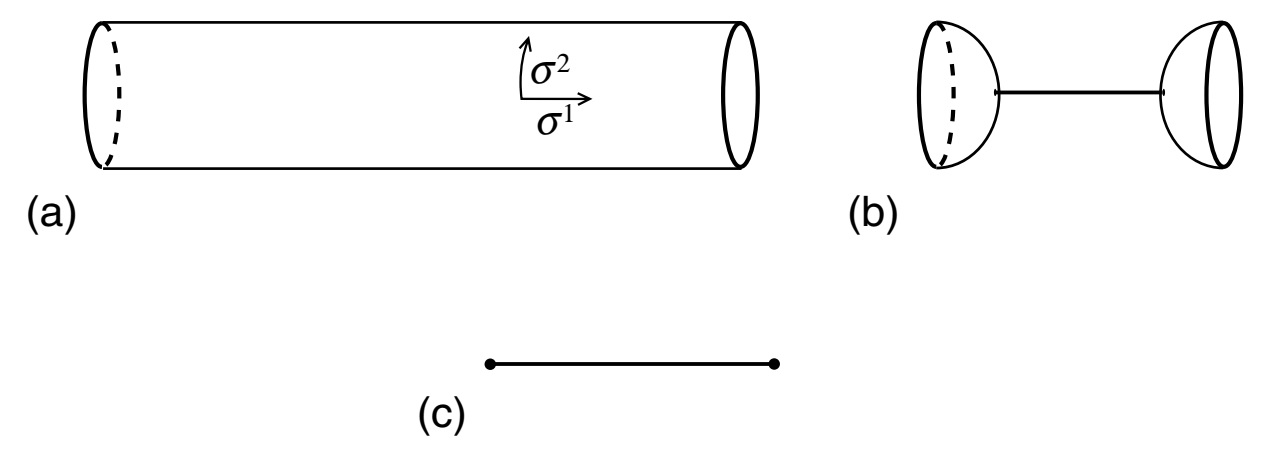
\includegraphics[width=0.8\textwidth]{figure/Fig7.1.jpg}\\
		\caption{(a) Cylinder in the small $t$ limit. (b) Amplitude decomposed into disk tadpole amplitudes and a closed string propagator. (c) Analogous field theory Feynman diagram. Heavy particles are analogous to tadpoles.}\label{Fig7.1} 
	\end{center}
\end{figure}

The $t \rightarrow 0$ limit is quite interesting. Unlike the torus, there is no modular group, and the integration limits cannot be truncated, so UV divergences of field theory still manifest. 
However, we will see that, like all divergences in string theory, this should actually be interpreted as a long-range effect. In the $t \rightarrow 0$ limit, this cylinder is very long, as shown in Figure \ref{Fig7.1}a. It looks like a closed string emerging from vacuum, propagating a certain distance, and then disappearing back into the vacuum. 
To make it more obvious, using the modular transformation \eqref{7.2.44} 
\begin{equation}
	\eta(\mi t)=t^{-1 / 2} \eta(\mi / t) \label{7.4.2} 
\end{equation}
and changing the variable to $s=\pi / t$, the result is 
\begin{equation}
	Z_{C_{2}}=\mi \frac{V_{26} n^{2}}{2 \pi(8 \pi^{2} \alpha^{\prime})^{13}} \int_{0}^{\infty} \dif s\: \eta(\mi s / \pi)^{-24} \:. \label{7.4.3} 
\end{equation}
Rescaling the metric by $1 / t$, the cylinder has a closed string circumference $2 \pi$, and the cylinder length is $s$. Expanding 
\begin{align}
	\eta(\mi s / \pi)^{-24} &=\exp (2 s) \prod_{n=1}^{\infty}[1-\exp (-2 n s)]^{-24} \nonumber \\
	&=\exp (2 s)+24+O(\exp (-2 s)) \:, \label{7.4.4} 
\end{align}
this is exactly the expected asymptotic form for an expansion in the complete closed string basis. 
In other words, if we consider $\sigma^{2}$ as worldsheet time and $\sigma^{1}$ as worldsheet distance, Figure \ref{Fig7.1}a is a very short open string loop. If we swap their roles, it is a very long closed string worldline, with both the beginning and end on the boundary circles. In Euclidean path integrals, both descriptions are usable and useful in different limits of moduli space. 

The leading order contribution to the vacuum amplitude comes from the closed string tachyon. 
This is uninteresting and can be defined through analytic continuation, 
\begin{equation}
	\int_{0}^{\infty} \dif s\:  \exp (\beta s) \equiv-\frac{1}{\beta} \:. \label{7.4.5} 
\end{equation}
The second term comes from massless closed string states, which even with continuation give a divergence of the form $1 / 0$. To see the origin of this divergence, dissociate the process as in Figure \ref{Fig7.1}b. As we saw in section \ref{sec:6.6}, there is a non-zero amplitude for a closed string vertex operator on a disk. 
The tadpole diagram corresponds to a closed string disappearing or appearing in the vacuum. In momentum space, the massless propagator is proportional to $1 / k^{2}$. Here, momentum conservation requires the momentum of the closed string emerging from vacuum to be zero, so the propagator diverges. 

The same type of divergence exists in quantum field theory. Consider a massless scalar field $\phi$ with a linear term for $\phi$ in the Lagrangian. Then there will be a vertex connected to only one propagator, and Figure \ref{Fig7.1}c exists. This divergence is due to the intermediate propagator being 
\begin{equation}
	\frac{1}{k^{2}}\bigg|_{k^{\mu}=0} \:. \label{7.4.6} 
\end{equation}
Since propagator poles correspond to long propagation distances in spacetime, this is a long-range (infrared) divergence. 
UV and IR divergences in quantum field theory have very different origins. UV divergences usually signal theory failure, requiring new physics at some short scale. IR divergences usually mean the question asked is wrong, or the method of expansion is wrong. This is the case here too. In general perturbation theory, we expand around $\phi(x)=0$ or some other field configuration. For the action 
\begin{equation}
	-\frac{1}{g^{2}} \int \dif^{d} x \: \left(\frac{1}{2} \partial_{\mu} \phi \partial^{\mu} \phi+g \Lambda \phi\right) \:, \label{7.4.7} 
\end{equation}
the equation of motion 
\begin{equation}
	\partial^{2} \phi=g \Lambda \label{7.4.8} 
\end{equation}
does not allow $\phi(x)=0$ as a solution. 
We must expand around a solution of \eqref{7.4.8}; any such solution must be position-dependent. The corresponding amplitude has no divergence, even if the right side is a perturbation (we introduced a suitable factor $g$ to the disk), because it is a singular perturbation. Specifically, the correct background breaks some Poincaré symmetries of the zero-order solution. 

The situation in string theory is the same. The disk tadpole is the source 
\begin{equation}
	-\Lambda \int \dif^{26} x\: (-G)^{1 / 2} \me^{-\tilde{\Phi}} \:, \label{7.4.9} 
\end{equation}
which is a source for the dilaton and metric. Expanding around the solution of the corresponding field equations (no longer constant) gives effective amplitudes. 
The details are somewhat complex and will be further discussed in Chapter \ref{cha:9}. Incidentally, in superstring theory, if the tree-level background is invariant under supersymmetry, it usually has no loop corrections. 

The pole \eqref{7.4.6} is the same type of divergence we encountered in tree amplitudes, corresponding to resonances propagating over long spacetime distances. If we add open string vertex operators at each end of the cylinder so that it represents an open string one-loop amplitude, the momentum $k^{\mu}$ flowing from one boundary to another is generally non-zero. 
Then the large $s$ limit \eqref{7.4.4} introduces the factor 
\begin{equation}
	\exp (-\alpha^{\prime} k^{2} s / 2)\:, \label{7.4.10} 
\end{equation}
and the divergence becomes a momentum pole, representing an open string scattering into a closed string intermediate state. Thus, as claimed in Chapter \ref{cha:3}, open string theory must simultaneously incorporate closed strings. The mechanism for removing UV divergences is different in open and closed strings. In closed strings, it is an effective truncation on modular integrals; in open strings, in the form of long spacetime distances, it is reinterpreted as a dangerous limit of moduli space. 

In \eqref{7.4.1}, we associated the path integral on the cylinder with the open string spectrum by cutting the path integral with $\sigma^{2}$ as time. 
It can also be obtained through closed strings, where $\sigma^{1}$ is time. Let $\sigma^{2}$ have period $2 \pi$ , with boundaries at $\sigma^{1}=0, s$. The closed string emerges in some state $|B\rangle$ at $\sigma^{1}=0$, and then disappears in the same way at $\sigma^{1}=s $. 
Introducing a measure insertion, the path integral is proportional to 
\begin{equation}
	\langle B|c_{0} b_{0} \exp [-s(L_{0}+\tilde{L}_{0})]| B\rangle \:. \label{7.4.11} 
\end{equation}
The fact that $\partial_{1} X^{\mu}, c^{1}$ and $b_{12}$ are zero on the boundary determines the state $|B\rangle$. 
In Hamiltonian form, they must annihilate $|B\rangle$; in terms of Laurent coefficients, 
\begin{equation}
	(\alpha_{n}^{\mu}+\tilde{\alpha}_{-n}^{\mu})|B\rangle=(c_{n}+\tilde{c}_{-n})|B\rangle=(b_{n}-\tilde{b}_{-n})|B\rangle=0, \quad \text { all } n\:. \label{7.4.12} 
\end{equation}
This gives 
\begin{equation}
	|B\rangle \propto (c_{0}+\tilde{c}_{0}) \exp \biggl[-\sum_{n=1}^{\infty}(n^{-1} \alpha_{-n} \cdot \tilde{\alpha}_{-n}+b_{-n} \tilde{c}_{-n}+\tilde{b}_{-n} c_{-n})\biggr]|0 ; 0\rangle \:. \label{7.4.13} 
\end{equation}
Using this in \eqref{7.4.11} yields \eqref{7.4.3}, with the normalization of $|B\rangle$ yet to be determined. This representation is very useful for analyzing the $t \rightarrow 0$ limit and closed string poles. 

By comparing string calculations with field theory, we can determine the disk tadpole $\Lambda$, but it will be more convenient to treat it as a special case of a more general result in the next chapter. 

\subsection*{Klein Bottle} 

The vacuum amplitude from the Klein bottle is 
\begin{align}
	Z_{K_{2}} &=\int_{0}^{\infty} \frac{\dif t}{4 t}\: \operatorname{Tr}_{\mathrm{c}}^{\prime} 
	\Bigl\{\Omega \exp [-2 \pi t (L_{0}+\tilde{L}_{0})]\Bigr\}  \nonumber \\
	&=\mi V_{d} \int_{0}^{\infty} \frac{\dif t}{4 t} \:(4 \pi^{2} \alpha^{\prime} t)^{-d / 2} 
	\sum_{i \in \mathscr{H}_{c}^{\perp}} \Omega_{i} \exp [-2 \pi t(h_{i}+\tilde{h}_{i}-2)] \:, \label{7.4.14} 
\end{align}
where the notation of the cylinder \eqref{7.4.1} is adopted. 
Compared with the torus of the oriented theory, this has an extra factor of $\frac{1}{2}$, coming from the projection operator $\frac{1}{2}(1+\Omega)$. For the same reason, the torus and cylinder amplitudes in unoriented theory both have an extra factor of $\frac{1}{2}$. This can also be seen as arising from the extra gauge invariance $w \rightarrow \bar{w}$. To calculate the trace in 26 flat dimensions, note that the only diagonal elements of $\Omega$ are those states where left-movers and right-movers are the same, and these states contribute $\Omega=+1 $. Thus, the trace is actually taken only on one side, which is the same as the open string amplitude, except that the weight is doubled because left and right contributions are identical. 
The result is 
\begin{equation}
	Z_{K_{2}} \rightarrow \mi V_{26} \int_{0}^{\infty} \frac{\dif t}{4 t}\: (4 \pi^{2} \alpha^{\prime} t)^{-13} \eta(2 \mi t)^{-24} \:. \label{7.4.15} 
\end{equation}

\begin{figure}[!htbp]
	\begin{center}
		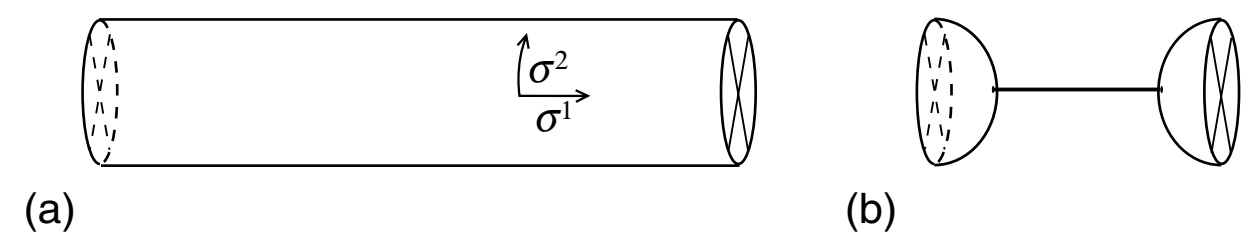
\includegraphics[width=0.8\textwidth]{figure/Fig7.2.jpg}\\
		\caption{(a) In the small $t$ limit, the Klein bottle becomes a cylinder with crosscaps at both ends. (b) Amplitude decomposed into $R P_{2}$ and $D_{2}$ tadpole amplitudes and a closed string propagator.}\label{Fig7.2} 
	\end{center}
\end{figure}

The modulus $t$ has the same range $0<t<\infty$ as for the cylinder, so the $t \rightarrow 0$ divergence is the same. 
Similarly, the $1 / 0$ pole can have a long-range explanation in the form of a closed string pole. To see this, consider the regions 
\begin{subequations} \label{7.4.16}
	\begin{align}
		&0 \leq \sigma^{1} \leq 2 \pi, \qquad 0 \leq \sigma^{2} \leq 2 \pi t  \:, \label{7.4.16a} \\
		&0 \leq \sigma^{1} \leq \pi, \qquad 0 \leq \sigma^{2} \leq 4 \pi t \:. \label{7.4.16b} 
	\end{align}		
\end{subequations}
Both are fundamental regions for the equivalence relation 
\begin{equation}
	w \cong w+2 \pi \cong-\bar{w}+2 \pi \mi t \label{7.4.17} 
\end{equation}
In \eqref{7.4.16a}, the left and right edges are periodically equivalent, while the top and bottom edges are equivalent after parity inversion, which explains the closed string loop with weight $\Omega $. For \eqref{7.4.16b}, the equivalence relation \eqref{7.4.17} simultaneously implies 
\begin{equation}
	w \cong w+4 \pi \mi t, \qquad w+\pi \cong-(\bar{w}+\pi)+2 \pi \mi t \:. \label{7.4.18} 
\end{equation}
It follows that the upper and lower edges of the region \eqref{7.4.16b} are periodically equivalent. After translating half the length of the left edge, the inversion through that edge is equivalent to itself. Similarly for the right edge: this is the definition of a crosscap. Thus we have the interpretation of Figure \ref{Fig7.2}a. Rescaling by $1 / 2 t$, the cylinder base length is $2 \pi$, height $s=\pi / 2 t$, and both ends are connected to crosscaps. 
After modular transformation, the amplitude becomes 
\begin{equation}
	Z_{K_{2}}=\mi \frac{2^{26} V_{26}}{4 \pi(8 \pi^{2} \alpha^{\prime})^{13}} \int_{0}^{\infty} \dif s\: \eta(\mi s / \pi)^{-24} \:. \label{7.4.19} 
\end{equation}
All discussions regarding divergences of the cylinder can be applied to the Klein bottle. The difference is that the tadpole diagrams come from the projective plane rather than the disk. 

\subsection*{M\"{o}bius Strip} 

For the M\"{o}bius strip, 
\begin{equation}
	Z_{M_{2}}=\mi V_{d} \int_{0}^{\infty} \frac{\dif t}{4 t} (8 \pi^{2} \alpha^{\prime} t)^{-d / 2} 
	\sum_{i \in \mathscr{H}_{0}^{\perp}} \Omega_{i} \exp [-2 \pi t(h_{i}-1)] \label{7.4.20} 
\end{equation}
It differs from the cylinder result only by $\Omega$ and the $\frac{1}{2}$ of the projection operator. 
In 26 flat dimensions, the effect of the operator $\Omega$ in the trace is: there is an extra $-1$ on even mass levels, plus a proper count of Chan-Paton factors. Thus, the trace of oscillators is 
\begin{equation}
	\exp (2 \pi t) \prod_{n=1}^{\infty}[1-(-1)^{n} \exp (-2 \pi n t)]^{-24}=\vartheta_{00}(0,2 \mi t)^{-12} \eta(2 \mi t)^{-12} \:. \label{7.4.21} 
\end{equation}
For $S O(n)$ theory, $\frac{1}{2} n(n+1)$ symmetric states have $\Omega=+1$, while $\frac{1}{2} n(n-1)$ antisymmetric states have $\Omega=-1$, giving a net contribution of $n$. For $S p(k)$ theory, it is the opposite, giving $-n$ (in our notation $n=2 k$ Chan-Paton states). 
Then the amplitude is 
\begin{equation}
	Z_{M_{2}}=\pm \mi n V_{26} \int_{0}^{\infty} \frac{\dif t}{4 t} \: (8 \pi^{2} \alpha^{\prime} t)^{-13} 
	\vartheta_{00}(0,2 \mi t)^{-12} \eta(2 \mi t)^{-12} \:. \label{7.4.22} 
\end{equation}


\begin{figure}[!htbp]
	\begin{center}
		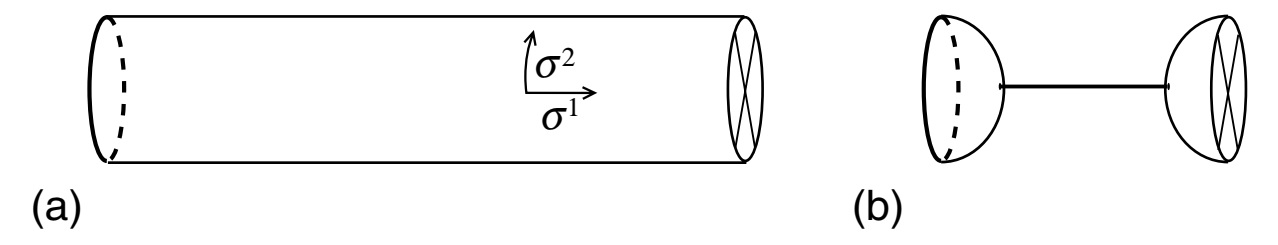
\includegraphics[width=0.8\textwidth]{figure/Fig7.3.jpg}\\
		\caption{(a) In the small $t$ limit, the Möbius strip becomes a cylinder with a crosscap at one end. (b) Amplitude decomposed into $D_{2}$ and $R P_{2}$ tadpole amplitudes and a closed string propagator.}\label{Fig7.3} 
	\end{center}
\end{figure}

By the same construction as for the Klein bottle, the M\"{o}bius strip can also be represented as a cylinder with a base, where only one end is a crosscap, as shown in Figure \ref{Fig7.3}a. The cylinder length is now $s=\pi / 4 t$. 
Through modular transformation, the amplitude is 
\begin{equation}
	Z_{M_{2}}=\pm 2 \mi n \frac{2^{13} V_{26}}{4 \pi(8 \pi^{2} \alpha^{\prime})^{13}}
	\int_{0}^{\infty} \dif s \: \vartheta_{00}(0,2 \mi s / \pi)^{-12} \eta(2 \mi s / \pi)^{-12} \:. \label{7.4.23} 
\end{equation}
As with the cylinder, this can also be written as an operator expression, with one boundary state in \eqref{7.4.11} replaced by a similar crosscap state $|C\rangle $. This is also a $t \rightarrow 0$ divergence; it corresponds to the process in Figure \ref{Fig7.3}a, with one end from the disk and the other from the projective plane. 
In unoriented theory, the divergences of these three surfaces combine into % 
\begin{equation}
	\mi \frac{24 V_{26}}{4 \pi(8 \pi^{2} \alpha^{\prime})^{13}}(2^{13} \mp n)^{2} \int_{0}^{\infty} \dif s\:. \label{7.4.24} % 
\end{equation}
That is, the total tadpole is proportional to $2^{13} \mp n $. % 
For the gauge group $SO(2^{13})=S O(8192)$, this is zero. The tadpole from the disk and the tadpole from the projective plane cancel each other. In bosonic string theory, this might not have special meaning, but in superstrings, there is indeed a similar cancellation for $SO(32)$. %
	% \setcounter{section}{0}
% \numberwithin{equation}{section}
% \numberwithin{figure}{section}
% \setcounter{chapter}{7}

\chapter{\texorpdfstring{Toroidal Compactification and $T$-duality}{8 Toroidal Compactification and $T$-duality}} \label{cha:8}
The realistic compactification of string theory will be the subject of the final chapters of Volume II, but let us first examine the simplest compactifications of string theory, where one or more dimensions are periodically identified. 
We first examine the same compactifications in field theory, which are encountered in the Kaluza-Klein unification of gauge interactions and gravity.
Then we extend this to string theory, where several new and intrinsic string phenomena arise: 
winding states, enhanced gauge symmetry, $T$-duality, and D-branes. We will also examine slightly more complex compactifications along this line, namely orbifolds and orientifolds.

\section{\texorpdfstring{Toroidal Compactification in Field Theory}{8.1 Toroidal Compactification in Field Theory}} \label{sec:8.1}

In general relativity, the geometry of spacetime is dynamical. The three spatial dimensions we see are extended, but they might have once been highly curled up. There is the logical possibility that there are still extra dimensions that remain very small.
In fact, this was proposed as early as 1914 as a way to unify the electromagnetic and gravitational fields into components of a single higher-dimensional field. Consider the 5-dimensional case, where $x^{4}$ is periodically identified:
\begin{equation}
	x^{4} \cong x^{4}+2 \pi R \:, \label{8.1.1}
\end{equation}
while the other $x^{\mu}$ for $\mu=0,\ldots,3$ are non-compact.
This is toroidal compactification, where the 5-dimensional metric splits into $G_{\mu \nu}, G_{\mu 4}$, and $G_{44} $. From a 4-dimensional perspective, these are a metric, a vector, and a scalar.

Let us examine this carefully: take the more general case of $D=d+1$ spacetime dimensions, where $x^{d}$ is periodic.
Parameterize the metric as:
\begin{equation}
	\dif s^{2}=G_{M N}^{D} \dif x^{M} \dif x^{N}=G_{\mu \nu} \dif x^{\mu} \dif x^{\nu}+G_{d d}(\dif x^{d}+A_{\mu} \dif x^{\mu})^{2} \:. \label{8.1.2}
\end{equation}
\begin{tcolorbox}[breakable]
	\begin{remark}
		\begin{align*}
			ds^2 &= G_{\mu\nu} \, dx^\mu dx^\nu + G_{dd} \left( dx^d dx^d + 2A_\mu dx^\mu dx^d + A_\mu A_\nu dx^\mu dx^\nu \right)\notag\\
			&= (G_{\mu\nu} + G_{dd} A_\mu A_\nu) \, dx^\mu dx^\nu + 2 G_{dd} A_\mu \, dx^\mu dx^d + G_{dd} \, dx^d dx^d\\
			&=G_{\mu\nu} \, dx^\mu dx^\nu + G_{dd} (A_\mu A_\nu\, dx^\mu dx^\nu+ 2 A_\mu \, dx^\mu dx^d + dx^d dx^d)
		\end{align*}
		Upon comparison with $G_{MN}^D$
		\vspace*{-20pt}
		\begin{equation*}
			G_{MN} = 
			\bordermatrix{
				& {\color{gray}\mu} & {\color{gray}d} \cr
				{\color{gray}\nu} & g_{\mu\nu} + G_{dd} A_\mu A_\nu & G_{dd} A_\mu \cr
				{\color{gray}d} & G_{dd} A_\nu & G_{dd} \cr
			}
		\end{equation*}
	\end{remark}
\end{tcolorbox}
Denote the metric of the entire $D$-dimensional spacetime as $G_{M N}^{D} $, and note that $G_{\mu \nu} \neq G_{\mu v}^{D} $; we use $G_{\mu \nu} $ to raise and lower indices in the $d$-dimensional action.
For now, only allow $G_{\mu \nu}, G_{d d}$ and $A_{\mu}$ to depend on $x^{\mu}$. \eqref{8.1.2} is the most general form of the metric that is invariant under translations of $x^{d}$. 
This form still allows for $d$-dimensional reparameterizations $x^{\prime \mu}(x^{\nu})$ and:
\begin{equation}
	x^{\prime d}=x^{d}+\lambda(x^{\mu}) \:. \label{8.1.3}
\end{equation}
Under this reparameterization:
\begin{equation}
	A_{\mu}^{\prime}=A_{\mu}-\partial_{\mu} \lambda \:, \label{8.1.4}
\end{equation}
so gauge transformations arise as part of the higher-dimensional coordinate group; this is the Kaluza-Klein mechanism. To see the effect of the $x^{d}$ dependence, consider a massless scalar $\phi$ in $D$ dimensions. For simplicity, take the metric in the compact dimension to be $G_{d d}=1$ and $G_{\mu d}=0$. The momentum in the periodic dimension is quantized, $p_{d}=n / R$.
Expand the dependence of $\phi$ on $x^{d}$ in a complete eigen-basis of Laplace Beltrami operator in compact dimensions as:
\begin{equation}
	\phi(x^{M})=\sum_{n=-\infty}^{\infty} \phi_{n}(x^{\mu}) \exp (\mi n x^{d} / R) \:. \label{8.1.5}
\end{equation}
The $D$-dimensional wave equation $\partial_{M} \partial^{M} \phi=\partial_{\mu}\partial^{\mu}\phi+\partial_d^2\phi=0$ becomes:
\begin{equation}
	\partial_{\mu} \partial^{\mu} \phi_{n}(x^{\mu})=\frac{n^{2}}{R^{2}} \phi_{n}(x^{\mu}) \:. \label{8.1.6}
\end{equation}
\begin{tcolorbox}[breakable]
	\begin{remark}
		Since we have introduced a gauge field on the worldsheet, the next step is to replace the ordinary derivative by the following covariant derivative:
		\begin{align*}
			\partial_{\mu} \to\mathcal{D}_{\mu}\equiv\partial_{\mu}+ip_dA_{\mu}
		\end{align*}
		To see this, we follow
		\begin{align*}
			g_{MN} &=
			\begin{pmatrix}
				g_{\mu\nu} +  A_\mu A_\nu &  A_\mu \\
				A_\nu & 1
			\end{pmatrix},
			\quad
			g^{MN} =
			\begin{pmatrix}
				g^{\mu\nu} & -A^\mu \\
				- A^\nu & 1 + A^2
			\end{pmatrix}
		\end{align*}
		The action can be simplified using $\Phi(x^\mu,x^d) = \phi(x^\mu)e^{i p_d x^d}, \quad \partial_d\Phi = i p_d \Phi$:
		\begin{align*}
			g^{MN}\partial_M \Phi \partial_N \Phi
			&= g^{\mu\nu}\partial_\mu\Phi\,\partial_\nu\Phi
			-2 A^\mu \partial_\mu\Phi\,\partial_d\Phi
			+\big(1+A^2\big)(\partial_d\Phi)^2
			\\[6pt]
			&= g^{\mu\nu}(\partial_\mu\phi)(\partial_\nu\phi)
			-2 i p_d A^\mu (\partial_\mu\phi)\phi
			- p^2_d\big(1+A^2\big)\phi^2
			\\[6pt]
			&= g^{\mu\nu}
			(\partial_\mu\phi + i p_d A_\mu \phi)
			(\partial_\nu\phi + i p_d A_\nu \phi)
			- p^2_d \phi^2
			\\[6pt]
			&= g^{\mu\nu} D_\mu \phi\, D_\nu \phi
			- p^2_d\phi^2
		\end{align*}
		Hence we arrive at:
		\[
		\mathcal{D}_\mu = \partial_\mu + i p_d A_\mu
		\]
	\end{remark}
\end{tcolorbox}
The modes $\phi_{n}$ of the $D$-dimensional field thus become an infinite tower of $d$-dimensional fields. For fields where $p_{d} $ is non-zero, the $d$-dimensional mass squared:
\begin{equation}
	-p^{\mu} p_{\mu}=\frac{n^{2}}{R^{2}} \label{8.1.7}
\end{equation}
is non-zero. When the energy is much smaller than $R^{-1}$, only the $x^{d}$ independence remains, and the physics is $d$-dimensional. When the energy exceeds $R^{-1}$, we see the Kaluza-Klein tower of states.
The charge corresponding to the Kaluza-Klein gauge invariance \eqref{8.1.3} is the $p_{d}$ momentum. In this simple example, all fields carrying Kaluza-Klein charge are massive. 
More generally, if there are also higher-spin fields and a curved background, there are also massless charged fields.

The effective action of massless fields is always an important topic. Define $G_{d d}=\me^{2 \sigma}$. The Ricci scalar of the metric \eqref{8.1.2} is:
\begin{equation}
	\bm{R}=\bm{R}_{d}-2 \me^{-\sigma} \nabla^{2} \me^{\sigma}-\frac{1}{4} \me^{2 \sigma} F_{\mu \nu} F^{\mu \nu} \:, \label{8.1.8}
\end{equation}
where $\bm{R}$ is constructed with $G_{M N}^{D}$, and $\bm{R}_{d}$ is constructed with $G_{\mu \nu} $.
\begin{tcolorbox}[breakable]
	\begin{proof}
			We begin with the $D$-dimensional metric for a base manifold $\mathcal{M}_d$ of dimension $d$ and a single extra dimension parameterized by $y$. The coordinate indices are denoted by $M, N = (\mu, y)$, where $\mu, \nu$ run over the $d$-dimensional base. The metric is given by:
			\begin{equation}
				ds_D^2 = g_{\mu\nu}(x) \, dx^\mu dx^\nu + e^{2\sigma(x)} \big( dy + A_\mu(x) \, dx^\mu \big)^2
			\end{equation}
			In matrix form,
			\[
			G_{MN} = \begin{pmatrix}
				g_{\mu\nu} + e^{2\sigma} A_\mu A_\nu & e^{2\sigma} A_\mu \\
				e^{2\sigma} A_\nu & e^{2\sigma}
			\end{pmatrix}.
			\]
			
			The inverse metric is
			\[
			G^{\mu\nu} = g^{\mu\nu}, \qquad
			G^{\mu d} = -A^\mu, \qquad
			G^{dd} = e^{-2\sigma} + A_\rho A^\rho,
			\]
			with $A^\mu = g^{\mu\nu} A_\nu$. To utilize Cartan's structural equations, we define a local orthonormal frame (the vielbeins or tetrads) $E^A$, such that the full metric is locally flat:
			\begin{equation}
				ds_D^2 = \eta_{AB} E^A \otimes E^B
			\end{equation}
			where $A, B$ are local Lorentz indices running over $(a, \hat{d})$. The metric signature is taken as mostly plus, so $\eta_{AB} = \text{diag}(-, +, +, \dots, +)$, with $\eta_{\hat{d}\hat{d}} = 1$. We define the basis 1-forms as:
			\begin{align}
				E^a &= e^a_\mu \, dx^\mu \label{eq:Ea} \\
				E^{\hat{d}} &= e^\sigma (dy + A_\mu \, dx^\mu) \equiv e^\sigma (dy + A) \label{eq:Ed}
			\end{align}
			where $g_{\mu\nu} = \eta_{ab} e^a_\mu e^b_\nu$. Note the inverse relation for the extra coordinate:
			\begin{equation}
				dy = e^{-\sigma} E^{\hat{d}} - A
			\end{equation}			
			Next, we compute the exterior derivatives $dE^A$ to prepare for Cartan's first structure equation. For the base dimensions, assuming the $d$-dimensional connection $\omega^a_{\ b}$ is torsion-free, we have:
			\begin{equation}
				dE^a = -\omega^a_{\ b} \wedge E^b
			\end{equation}
			
			For the extra dimension, we take the exterior derivative of \eqref{eq:Ed}. Using the Leibniz rule and the property $d^2 = 0$, we find:
			\begin{equation}
				dE^{\hat{d}} = d(e^\sigma) \wedge (dy + A) + e^\sigma dA
			\end{equation}
			We expand the scalar differential $d(e^\sigma) = e^\sigma d\sigma = e^\sigma \partial_b \sigma E^b$. The exterior derivative of the gauge potential defines the field strength 2-form: 
			\begin{equation}
				dA = \frac{1}{2} F_{\mu\nu} dx^\mu \wedge dx^\nu = \frac{1}{2} F_{bc} E^b \wedge E^c
			\end{equation}
			Substituting these into our expression for $dE^{\hat{d}}$, and replacing $(dy + A)$ with $e^{-\sigma}E^{\hat{d}}$, we obtain:
			\begin{align}
				dE^{\hat{d}} &= (e^\sigma \partial_b \sigma E^b) \wedge (e^{-\sigma} E^{\hat{d}}) + e^\sigma \left( \frac{1}{2} F_{bc} E^b \wedge E^c \right) \nonumber \\
				&= \partial_b \sigma E^b \wedge E^{\hat{d}} + \frac{1}{2} e^\sigma F_{bc} E^b \wedge E^c
			\end{align}
				
			Cartan's first structure equation dictates that the torsion 2-form vanishes for the Levi-Civita connection:
			\begin{equation}
				dE^A + \hat{\Omega}^A_{\ B} \wedge E^B = 0
			\end{equation}
			Because we are working in an orthonormal frame with constant $\eta_{AB}$, the connection 1-forms are antisymmetric: $\hat{\Omega}_{AB} = -\hat{\Omega}_{BA}$. We set $A = \hat{d}$ in the first structure equation:
			\begin{equation}
				dE^{\hat{d}} + \hat{\Omega}^{\hat{d}}_{\ b} \wedge E^b = 0 \implies \hat{\Omega}^{\hat{d}}_{\ b} \wedge E^b = -dE^{\hat{d}}
			\end{equation}
			Since $\eta_{\hat{d}\hat{d}} = 1$, we have $\hat{\Omega}^{\hat{d}}_{\ b} = \hat{\Omega}_{\hat{d}b}$. Substituting our result for $dE^{\hat{d}}$:
			\begin{equation}
				\hat{\Omega}_{\hat{d}b} \wedge E^b = -\frac{1}{2} e^\sigma F_{bc} E^b \wedge E^c - \partial_b \sigma E^b \wedge E^{\hat{d}}
			\end{equation}
			By proposing a general ansatz $\hat{\Omega}_{\hat{d}b} = K_{bc} E^c + V_b E^{\hat{d}}$ and matching the wedge products, we can isolate $\hat{\Omega}_{\hat{d}b}$:
			\begin{equation}
				\hat{\Omega}_{\hat{d}b} = \frac{1}{2} e^\sigma F_{bc} E^c + \partial_b \sigma E^{\hat{d}}
			\end{equation}
			By antisymmetry, swapping the local Lorentz indices yields:
			\begin{equation}
				\hat{\Omega}_{a\hat{d}} = -\hat{\Omega}_{\hat{d}a} = -\frac{1}{2} e^\sigma F_{ac} E^c - \partial_a \sigma E^{\hat{d}}
			\end{equation}
			Now we set $A = a$ in the structure equation:
			\begin{equation}
				dE^a + \hat{\Omega}^a_{\ b} \wedge E^b + \hat{\Omega}^a_{\ \hat{d}} \wedge E^{\hat{d}} = 0
			\end{equation}
			We subtract the pure $d$-dimensional torsion-free condition $dE^a + \omega^a_{\ b} \wedge E^b = 0$, which leaves:
			\begin{equation}
				(\hat{\Omega}^a_{\ b} - \omega^a_{\ b}) \wedge E^b = -\hat{\Omega}^a_{\ \hat{d}} \wedge E^{\hat{d}}
			\end{equation}
			We raise the index on our previously found connection, $\hat{\Omega}^a_{\ \hat{d}} = \eta^{ac}\hat{\Omega}_{c\hat{d}} = -\frac{1}{2} e^\sigma F^a_{\ c} E^c - \partial^a \sigma E^{\hat{d}}$. Substituting this into the right-hand side:
			\begin{align}
				-\hat{\Omega}^a_{\ \hat{d}} \wedge E^{\hat{d}} &= - \left( -\frac{1}{2} e^\sigma F^a_{\ c} E^c - \partial^a \sigma E^{\hat{d}} \right) \wedge E^{\hat{d}} \nonumber \\
				&= \frac{1}{2} e^\sigma F^a_{\ c} E^c \wedge E^{\hat{d}} \nonumber \\
				&= -\frac{1}{2} e^\sigma F^a_{\ b} E^{\hat{d}} \wedge E^b
			\end{align}
			where we renamed the dummy index $c \to b$ and used the antisymmetry of the wedge product $E^b \wedge E^{\hat{d}} = -E^{\hat{d}} \wedge E^b$. Matching the coefficients with the left-hand side yields the modified base connection:
			\begin{equation}
				\hat{\Omega}^a_{\ b} = \omega^a_{\ b} - \frac{1}{2} e^\sigma F^a_{\ b} E^{\hat{d}} \implies \hat{\Omega}_{ab} = \omega_{ab} - \frac{1}{2} e^\sigma F_{ab} E^{\hat{d}}
			\end{equation}
			
			The curvature 2-forms $\hat{\Theta}_{AB}$ are generated by Cartan's second structure equation:
			\begin{equation}
				\hat{\Theta}_{AB} = d\hat{\Omega}_{AB} + \hat{\Omega}_{AC} \wedge \hat{\Omega}^C_{\ B}
			\end{equation}
			The components of the Riemann tensor are extracted via $\hat{\Theta}_{AB} = \frac{1}{2} \hat{R}_{ABCD} E^C \wedge E^D$.
			
			We expand the structure equation for indices $A=a, B=b$:
			\begin{equation}
				\hat{\Theta}_{ab} = d\hat{\Omega}_{ab} + \hat{\Omega}_{ac} \wedge \hat{\Omega}^c_{\ b} + \hat{\Omega}_{a\hat{d}} \wedge \hat{\Omega}^{\hat{d}}_{\ b}
			\end{equation}
			We are only interested in terms proportional to $E^c \wedge E^d$, so we project out any terms containing $E^{\hat{d}}$. Note that $d$ and $\hat{d}$ are fundamentally different, while the latter is extra dimension index the prior is dummy index.
			
			1. \textbf{The $d\hat{\Omega}_{ab}$ term:}
			\begin{equation}
				d\hat{\Omega}_{ab} = d\omega_{ab} - \frac{1}{2} d(e^\sigma F_{ab}) \wedge E^{\hat{d}} - \frac{1}{2} e^\sigma F_{ab} dE^{\hat{d}}
			\end{equation}
			The purely base part comes entirely from $d\omega_{ab}$ and the $E^c \wedge E^d$ component of $dE^{\hat{d}}$:
			\begin{equation}
				\left. d\hat{\Omega}_{ab} \right|_{\text{base}} = d\omega_{ab} - \frac{1}{2} e^\sigma F_{ab} \left( \frac{1}{2} e^\sigma F_{cd} E^c \wedge E^d \right) = d\omega_{ab} - \frac{1}{4} e^{2\sigma} F_{ab} F_{cd} E^c \wedge E^d
			\end{equation}
			
			2. \textbf{The $\hat{\Omega}_{ac} \wedge \hat{\Omega}^c_{\ b}$ term:}
			The projection of this term onto the base leaves only the standard $d$-dimensional connection:
			\begin{equation}
				\left. \hat{\Omega}_{ac} \wedge \hat{\Omega}^c_{\ b} \right|_{\text{base}} = \omega_{ac} \wedge \omega^c_{\ b}
			\end{equation}
			Combining $d\omega_{ab} + \omega_{ac} \wedge \omega^c_{\ b}$ forms the standard $d$-dimensional curvature 2-form $\Theta_{ab} = \frac{1}{2} R_{abcd} E^c \wedge E^d$.
			
			3. \textbf{The $\hat{\Omega}_{a\hat{d}} \wedge \hat{\Omega}^{\hat{d}}_{\ b}$ term:}
			Using $\hat{\Omega}^{\hat{d}}_{\ b} = \hat{\Omega}_{\hat{d}b}$, we multiply the purely spatial parts of the connections derived earlier:
			\begin{align}
				\left. \hat{\Omega}_{a\hat{d}} \wedge \hat{\Omega}^{\hat{d}}_{\ b} \right|_{\text{base}} &= \left( -\frac{1}{2} e^\sigma F_{ac} E^c \right) \wedge \left( \frac{1}{2} e^\sigma F_{bd} E^d \right) \nonumber \\
				&= -\frac{1}{4} e^{2\sigma} F_{ac} F_{bd} E^c \wedge E^d
			\end{align}
			To properly extract the Riemann tensor, we explicitly antisymmetrize $c$ and $d$:
			\begin{equation}
				-\frac{1}{4} e^{2\sigma} F_{ac} F_{bd} E^c \wedge E^d = -\frac{1}{8} e^{2\sigma} (F_{ac} F_{bd} - F_{ad} F_{bc}) E^c \wedge E^d
			\end{equation}
			
			Summing these contributions and equating to $\frac{1}{2}\hat{R}_{abcd} E^c \wedge E^d$, we multiply by 2 to isolate the Riemann tensor:
			\begin{equation} \label{eq:Rabcd}
				\hat{R}_{abcd} = R_{abcd} - \frac{1}{2} e^{2\sigma} F_{ab} F_{cd} - \frac{1}{4} e^{2\sigma} (F_{ac} F_{bd} - F_{ad} F_{bc})
			\end{equation}
			We expand the structure equation for indices $A=a, B=\hat{d}$:
			\begin{equation}
				\hat{\Theta}_{a\hat{d}} = d\hat{\Omega}_{a\hat{d}} + \hat{\Omega}_{ac} \wedge \hat{\Omega}^c_{\ \hat{d}}
			\end{equation}
			Here, we specifically want the coefficient of $E^b \wedge E^{\hat{d}}$ to find $\hat{R}_{a\hat{d}b\hat{d}}$.
			
			1. \textbf{The $d\hat{\Omega}_{a\hat{d}}$ term:}
			\begin{equation}
				d\hat{\Omega}_{a\hat{d}} = d\left( -\frac{1}{2} e^\sigma F_{ac} E^c - \partial_a \sigma E^{\hat{d}} \right)
			\end{equation}
			Focusing on the terms generating $E^b \wedge E^{\hat{d}}$:
			\begin{align}
				-d(\partial_a \sigma) \wedge E^{\hat{d}} &= -\partial_b \partial_a \sigma E^b \wedge E^{\hat{d}} \\
				-\partial_a \sigma dE^{\hat{d}} &\supset -\partial_a \sigma (\partial_b \sigma E^b \wedge E^{\hat{d}}) = -\partial_a \sigma \partial_b \sigma E^b \wedge E^{\hat{d}}
			\end{align}
			
			2. \textbf{The $\hat{\Omega}_{ac} \wedge \hat{\Omega}^c_{\ \hat{d}}$ term:}
			\begin{equation}
				\hat{\Omega}_{ac} \wedge \hat{\Omega}^c_{\ \hat{d}} = \left( \omega_{ac} - \frac{1}{2} e^\sigma F_{ac} E^{\hat{d}} \right) \wedge \left( -\frac{1}{2} e^\sigma F^c_{\ b} E^b - \partial^c \sigma E^{\hat{d}} \right)
			\end{equation}
			The cross terms generating $E^b \wedge E^{\hat{d}}$ are twofold. First, the base connection wedge the gradient of $\sigma$ combines with the partial derivatives above to form the covariant derivative (the Hessian):
			\begin{equation}
				-\partial_b \partial_a \sigma E^b \wedge E^{\hat{d}} + \omega_{ac} \wedge (-\partial^c \sigma E^{\hat{d}}) = -\nabla_b \nabla_a \sigma E^b \wedge E^{\hat{d}}
			\end{equation}
			Second, the cross term between the two field strengths yields:
			\begin{equation}
				\left( -\frac{1}{2} e^\sigma F_{ac} E^{\hat{d}} \right) \wedge \left( -\frac{1}{2} e^\sigma F^c_{\ b} E^b \right) = \frac{1}{4} e^{2\sigma} F_{ac} F^c_{\ b} E^{\hat{d}} \wedge E^b = -\frac{1}{4} e^{2\sigma} F_{ac} F^c_{\ b} E^b \wedge E^{\hat{d}}
			\end{equation}
			Summing these contributions gives the mixed Riemann component:
			\begin{equation} \label{eq:Rmixed}
				\hat{R}_{a\hat{d}b\hat{d}} = -\nabla_b \nabla_a \sigma - \partial_a \sigma \partial_b \sigma - \frac{1}{4} e^{2\sigma} F_{ac} F_b^{\ c}
			\end{equation}
			
			The full $D$-dimensional Ricci scalar is the full trace of the Riemann tensor over all indices:
			\begin{equation}
				\hat{R} = \eta^{ac}\eta^{bd} \hat{R}_{abcd} + 2 \eta^{ab} \hat{R}_{a\hat{d}b\hat{d}}= \hat{R}^{(d)} + 2 \eta^{ab}\eta^{\hat{d}\hat{d}} \hat{R}_{a\hat{d}b\hat{d}} \equiv \hat{R}^{(d)} + 2 \hat{R}_{a\hat{d}}^{\ \ \ \ a\hat{d}}
			\end{equation}
			First, we contract \eqref{eq:Rabcd} with $\eta^{bd}$ to find the intermediate Ricci tensor $\hat{R}_{ac}$:
			\begin{equation}
				\hat{R}_{ac} = R_{ac} - \frac{1}{2} e^{2\sigma} F_{ab} F_c^{\ b} - \frac{1}{4} e^{2\sigma} (F_{ac} F_b^{\ b} - F_{ad} \eta^{bd} F_{bc})
			\end{equation}
			Because the field strength is antisymmetric, the trace vanishes ($F_b^{\ b} = 0$), and we can rewrite $-F_{ad} \eta^{bd} F_{bc} = -F_a^{\ b} F_{bc} = +F_{ab} F_c^{\ b}$. Thus:
			\begin{equation}
				\hat{R}_{ac} = R_{ac} - \frac{1}{2} e^{2\sigma} F_{ab} F_c^{\ b} - \frac{1}{4} e^{2\sigma} (F_{ab} F_c^{\ b}) = R_{ac} - \frac{3}{4} e^{2\sigma} F_{ab} F_c^{\ b}
			\end{equation}
			Contracting with $\eta^{ac}$ to construct the scalar, and defining $F^2 \equiv F_{ab} F^{ab}$, we get:
			\begin{equation}
				\hat{R}^{(d)} = R_d - \frac{3}{4} e^{2\sigma} F_{ab} F^{ab} = R_d - \frac{3}{4} e^{2\sigma} F^2
			\end{equation}
			Next, we contract \eqref{eq:Rmixed} with $\eta^{ab}$. We must carefully handle the field strength term:
			\begin{equation}
				\eta^{ab} \left( -\frac{1}{4} e^{2\sigma} F_{ac} F_b^{\ c} \right) = -\frac{1}{4} e^{2\sigma} F_c^{\ b} F_b^{\ c} = -\frac{1}{4} e^{2\sigma} (-F_{bc} F^{bc}) = +\frac{1}{4} e^{2\sigma} F^2
			\end{equation}
			Therefore, the trace of the mixed component is:
			\begin{equation}
				\hat{R}_{a\hat{d}}^{\ \ \ \ a\hat{d}} = -\nabla^2 \sigma - (\partial \sigma)^2 + \frac{1}{4} e^{2\sigma} F^2
			\end{equation}
			We sum the base and mixed traces:
			\begin{align}
				\hat{R} &= \left( R_d - \frac{3}{4} e^{2\sigma} F^2 \right) + 2 \left( -\nabla^2 \sigma - (\partial \sigma)^2 + \frac{1}{4} e^{2\sigma} F^2 \right) \nonumber \\
				&= R_d - 2 \nabla^2 \sigma - 2 (\partial \sigma)^2 - \frac{1}{4} e^{2\sigma} F^2
			\end{align}
			Finally, we can condense the scalar derivatives into a single total derivative term. Consider the covariant d'Alembertian of $e^\sigma$:
			\begin{equation}
				\nabla_a (e^\sigma) = e^\sigma \partial_a \sigma \implies \nabla^2 (e^\sigma) = \nabla^a (e^\sigma \partial_a \sigma) = e^\sigma \nabla^2 \sigma + e^\sigma (\partial_a \sigma \partial^a \sigma)
			\end{equation}
			Multiplying this identity by $2e^{-\sigma}$ yields exactly the combination in our Ricci scalar:
			\begin{equation}
				2e^{-\sigma} \nabla^2 (e^\sigma) = 2 \nabla^2 \sigma + 2 (\partial \sigma)^2
			\end{equation}
			Substituting this back into the full trace, we arrive at the final result:
			\begin{equation}
				\boxed{ \hat{R} = R_d - 2 e^{-\sigma} \nabla^2 (e^\sigma) - \frac{1}{4} e^{2\sigma} F_{\mu\nu} F^{\mu\nu} }
			\end{equation}
	\end{proof}
\end{tcolorbox}
The graviton-dilaton action \eqref{3.7.20} becomes:
\begin{align}
	\bm{S}_{1} &= \frac{1}{2 \kappa_{0}^{2}} \int \dif^{D} x \: (-G_{D})^{1/2} \me^{-2 \Phi}(\bm{R}
	+4 \nabla_{\mu} \Phi \nabla^{\mu} \Phi) \nonumber \\
	&= \frac{\pi R}{\kappa_{0}^{2}} \int \dif^{d} x\: (-G_{d})^{1/2} \me^{-2 \Phi+\sigma}\left(\bm{R}_{d}-4 \partial_{\mu} \Phi \partial^{\mu} \sigma+
	4 \partial_{\mu} \Phi \partial^{\mu} \Phi-\frac{1}{4} \me^{2 \sigma} F_{\mu \nu} F^{\mu \nu}\right)\nonumber \\
	&= \frac{\pi R}{\kappa_{0}^{2}} \int  \dif^{d} x \:(-G_{d})^{1 / 2} \me^{-2 \Phi_{d}} \left(\bm{R}_{d}-\partial_{\mu} \sigma \partial^{\mu} \sigma+4 \partial_{\mu} \Phi_{d} \partial^{\mu} \Phi_{d}-\frac{1}{4} \me^{2 \sigma} F_{\mu \nu} F^{\mu \nu}\right) \:, \label{8.1.9}
\end{align}
which gives the kinetic terms for all massless fields.
Here $G_{d}$ is the determinant of $G_{\mu \nu}$, and $\Phi_{d}=\Phi-\sigma / 2$ is the effective $d$-dimensional dilaton. The sign error of the dilaton kinetic term is fictitious, because the mixing of the graviton with the metric trace must also be considered. The simplest way to achieve this is through the Weyl transformation in \eqref{3.7.25}.

The field equations do not determine the radius of the compact dimension. For any values of $\Phi$ and $\sigma $, the flat metric and constant dilaton are solutions. In other words, $\Phi$ and $\sigma$ have no potential, so these fields must be massless, much like Goldstone bosons. Different values of $\Phi$ and $\sigma$ mark degenerate configurations (or states of the quantum theory), and if the field in the state varies slowly, its energy comes only from the gradient. It differs from the Goldstone phenomenon in that the degenerate states are not related to each other by any symmetry.
In this bosonic theory, the degeneracy is accidental, and the one-loop energy discussed in the previous section breaks this degeneracy. In supersymmetric theories, the existence of physically inequivalent but degenerate vacua is quite common and plays a significant role in understanding dynamics. The fields used to mark inequivalent vacua are called moduli. In nature, supersymmetry breaking almost necessarily endows all moduli with mass; otherwise, they would transmit infinite long-range forces of gravitational magnitude.
\begin{tcolorbox}[breakable]
	\begin{remark}
In string theory, there are no fixed “given” constants; all physical couplings arise as vacuum expectation values (VEVs) of dynamical background fields, which themselves originate from condensation of string modes. In this sense, the space of couplings is the space of possible consistent background configurations of the string.

The moduli space is the subspace of this larger parameter space for which the worldsheet theory remains conformally invariant, i.e.\ where all $\beta$-functions vanish ($\beta=0$). Since the vanishing of $\beta$-functions is equivalent to the target-space equations of motion, every point in moduli space corresponds to a fully consistent string vacuum. Thus, moduli space should be understood as the locus of exact CFT backgrounds inside the full space of possible couplings/background fields.

In the low-energy effective theory, the background fields appear as spacetime fields whose zero-modes determine the couplings. In particular, the internal components of the metric $G_{ij}$ and the Kalb--Ramond field $B_{ij}$ along compact directions become scalar fields in lower dimensions upon dimensional reduction, whose VEVs parameterize deformations of the compactification.

As a concrete example, consider a compact direction labeled by $d$. The internal metric component $G_{dd}$ determines a geometric parameter such as the radius of a circle via $G_{dd} \sim R^2$. This component is therefore not merely a fixed entry of the metric, but a coupling of the two-dimensional sigma model, i.e.\ a background field expectation value sourced by string condensation in that mode.

When we expand around such a background, fluctuations of $G_{dd}(x)$ appear as scalar fields in the lower-dimensional effective theory. These fluctuations correspond to motion along directions in moduli space, and hence are massless moduli as long as conformal invariance is preserved. By contrast, fluctuations involving non-compact components $G_{\mu\nu}$ behave as ordinary propagating spacetime fields and are analyzed via standard perturbation theory.

Thus, only those components of background fields corresponding to exactly marginal deformations define coordinates on moduli space, while their VEVs fix the effective couplings of the lower-dimensional theory. Whether these directions remain flat or are lifted corresponds to the problem of moduli stabilization.
	\end{remark}
\end{tcolorbox}
Defining $A_{\mu}=R \tilde{A}_{\mu}$, the covariant derivative is:
\begin{equation}
	\partial_{M}\equiv\partial_{\mu}+\mi p_{d} A_{\mu}=\partial_{\mu}+\mi n \tilde{A}_{\mu} \:, \label{8.1.10}
\end{equation}
which makes the charge an integer.
The definitions of $d$-dimensional gauge coupling and gravitational coupling are as follows. The coefficient of $\tilde{F}_{\mu \nu} \tilde{F}^{\mu \nu}$ in the Lagrangian density is defined as $-1 / 4 g_{d}^{2}$, and the coefficient of $\bm{R}_{d}$ is defined as $1 / 2 \kappa_{d}^{2}$.
In terms of gravitational coupling, the gauge coupling is written as:
\begin{equation}
	g_{d}^{2}=\frac{\kappa_{0}^{2} \me^{2 \Phi_{d}}}{\pi R^{3} \me^{2 \sigma}}=\frac{2 \kappa_{d}^{2}}{\rho^{2}} \:. \label{8.1.11}
\end{equation}
The relationship between $d$-dimensional and $D$-dimensional gravitational couplings is:
\begin{equation}
	\frac{1}{\kappa_{d}^{2}}=\frac{2 \pi \rho}{\kappa^{2}} \:, \label{8.1.12}
\end{equation}
where $2 \pi \rho$ is the volume of the compact dimension.
\begin{tcolorbox}
	\begin{remark}
		\begin{itemize}
			\item $1 / g_{d}^{2}$ has a factor of $R^{2}$ contributed by the definition $A_{\mu}=R \tilde{A}_{\mu}$. Other contributions come from \eqref{8.1.9}, and combined with $\rho=R\me^{\sigma}$, this gives \eqref{8.1.11}.
			\item According to \eqref{8.1.9} and the definition, $1 / 2 \kappa_{d}^{2}=\frac{\pi R \me^{-2 \Phi_d}}{\kappa_{0}^{2}}$.
			The $D$-dimensional gravitational coupling is $\frac{1}{2 \kappa^{2}}=\frac{\me^{-2 \Phi}}{2 \kappa_{0}^{2}}$, which yields \eqref{8.1.12}.
		\end{itemize}
	\end{remark}
\end{tcolorbox}

By extending the Kaluza-Klein mechanism, antisymmetric tensors can also provide gauge symmetry.
Divide $B_{M N}$ into $B_{\mu \nu}$ and $A_{\mu}^{\prime}=B_{d \mu}$. The gauge parameter $\zeta_{M}$ in \eqref{3.7.7} is divided into the $d$-dimensional antisymmetric tensor transformation $\zeta_{\mu}$ and the ordinary gauge invariant $\zeta_{d}$. The gauge field is $B_{d \mu}$, and the field strength is $H_{d \mu \nu}$.
The antisymmetric tensor action becomes:
\begin{align}
	\bm{S}_{2} &=-\frac{1}{24 \kappa_{0}^{2}} \int \dif^{D} x \:(-G_{D})^{1 / 2} \me^{-2 \Phi} H_{M N L} H^{M N L} \nonumber \\
	&=-\frac{\pi R}{12 \kappa_{0}^{2}} \int \dif^{d} x \: (-G_{d})^{1/2} \me^{-2 \Phi_{d}}
	\Bigl(\tilde{H}_{\mu \nu \lambda} \tilde{H}^{\mu \nu \lambda}+3 \me^{-2 \sigma} H_{d \mu \nu} H_{d}^{\mu \nu}\Bigr) \:. \label{8.1.13}
\end{align}
We defined:
\begin{equation}
	\tilde{H}_{\mu \nu \lambda}=(\partial_{\mu} B_{\nu \lambda}-A_{\mu} H_{d \nu \lambda})+\text{cyclic permutations} \:. \label{8.1.14}
\end{equation}
\begin{tcolorbox}[breakable]
	\begin{proof}		 
	We begin with a $D$-dimensional spacetime where the extra dimension $x^d$ is compactified. The standard Kaluza-Klein ansatz for the $D$-dimensional metric $G_{MN}$ is given by
	\begin{equation}
		ds^2_D = G_{\mu\nu} dx^\mu dx^\nu + e^{2\sigma} (dx^d + A_\mu dx^\mu)^2 \, ,
	\end{equation}
	where $G_{\mu\nu}$ is the $d$-dimensional metric, $A_\mu$ is the Kaluza-Klein gauge field, and $\sigma$ is the radion field. Written as a block matrix, the metric takes the form
	\begin{equation}
		G_{MN} = \begin{pmatrix} G_{\mu\nu} + e^{2\sigma} A_\mu A_\nu & e^{2\sigma} A_\mu \\ e^{2\sigma} A_\nu & e^{2\sigma} \end{pmatrix} \, .
	\end{equation}
	
	The determinant of this matrix can be computed using the standard block matrix identity, yielding $\det(G_D) = e^{2\sigma} \det(G_{\mu\nu})$, which implies $\sqrt{-G_D} = e^\sigma \sqrt{-G_d}$. To maintain the standard form of the gravitational action in the lower-dimensional Einstein frame, we must define the $d$-dimensional dilaton $\Phi_d$ by shifting the $D$-dimensional dilaton $\Phi$ according to $\Phi_d = \Phi - \frac{1}{2}\sigma$. Consequently, the integration measure transforms exactly as required:
	\begin{equation}
		\sqrt{-G_D} e^{-2\Phi} = (e^\sigma \sqrt{-G_d}) (e^{-2\Phi_d} e^{-\sigma}) = \sqrt{-G_d} e^{-2\Phi_d} \, .
	\end{equation}
	
	Next, we expand the kinetic term $H_{MNL} H^{MNL}$. This requires the $D$-dimensional inverse metric $\tilde{G}^{MN}$, whose non-zero components are $\tilde{G}^{\mu\nu} = G^{\mu\nu}$, $\tilde{G}^{\mu d} = -A^\mu$, and $\tilde{G}^{dd} = e^{-2\sigma} + A_\alpha A^\alpha$. The 3-form field strength $H_{MNL}$ is totally antisymmetric. Because the field does not depend on the compactified coordinate $x^d$ (so $\partial_d = 0$), the non-zero components are $H_{\mu\nu\lambda}$ and $H_{d\mu\nu} = \partial_\mu B_{\nu d} - \partial_\nu B_{\mu d}$. We contract the indices of $H_D^2 = H_{MNL} H_{PQR} \tilde{G}^{MP} \tilde{G}^{NQ} \tilde{G}^{LR}$ and group the terms by the number of compact indices involved. Summing the contributions from terms with zero, one, and two $d$ indices respectively, we obtain the raw expansion of the kinetic term:
	\begin{equation}
		H_D^2 = H_{\mu\nu\lambda} H^{\mu\nu\lambda} - 6 A^\lambda H_{\mu\nu\lambda} H_d^{\mu\nu} + 3 (e^{-2\sigma} + A^2) H_{d\mu\nu} H_d^{\mu\nu} + 6 A^\mu A^\nu H_{d\mu\lambda} H_{d\nu}^{\ \ \lambda} \, .
		\label{eq:raw_kinetic}
	\end{equation}
	
	This expression can be neatly recombined by introducing the gauge-invariant field strength for the 2-form under the Kaluza-Klein $U(1)$ symmetry, defined as
	\begin{equation}
		\tilde{H}_{\mu\nu\lambda} = H_{\mu\nu\lambda} - 3 A_{[\mu} H_{d|\nu\lambda]} = H_{\mu\nu\lambda} - A_\mu H_{d\nu\lambda} - A_\nu H_{d\lambda\mu} - A_\lambda H_{d\mu\nu} \, .
	\end{equation}
	Squaring this invariant field strength directly in $d$ dimensions gives
	\begin{equation}
		\tilde{H}_{\mu\nu\lambda} \tilde{H}^{\mu\nu\lambda} = H_{\mu\nu\lambda} H^{\mu\nu\lambda} - 6 A^\lambda H_{\mu\nu\lambda} H_d^{\mu\nu} + 3 A^2 H_{d\mu\nu} H_d^{\mu\nu} + 6 A^\mu A^\nu H_{d\mu\lambda} H_{d\nu}^{\ \ \lambda} \, .
	\end{equation}
	
	Comparing this to equation \eqref{eq:raw_kinetic}, it perfectly matches all the $A$-dependent terms. Subtracting this from our raw $H_D^2$ expansion isolates the radion-scaled term, simplifying the higher-dimensional kinetic term to
	\begin{equation}
		H_D^2 = \tilde{H}_{\mu\nu\lambda} \tilde{H}^{\mu\nu\lambda} + 3 e^{-2\sigma} H_{d\mu\nu} H_d^{\mu\nu} \, .
	\end{equation}
	
	Finally, we substitute these geometric and kinetic results back into the original action $S_2$. The integration over the $D$-dimensional spacetime splits into the non-compact dimensions and the compact dimension $S^1$. Integrating over the circle evaluates to its circumference, $\int_0^{2\pi R} dx^d = 2\pi R$. The action becomes
	\begin{align}
		S_2 &= -\frac{1}{24\kappa_0^2} \int d^D x \sqrt{-G_D} e^{-2\Phi} H_{MNL} H^{MNL} \nonumber \\
		&= -\frac{1}{24\kappa_0^2} (2\pi R) \int d^d x \sqrt{-G_d} e^{-2\Phi_d} \left( \tilde{H}_{\mu\nu\lambda} \tilde{H}^{\mu\nu\lambda} + 3 e^{-2\sigma} H_{d\mu\nu} H_d^{\mu\nu} \right) \, .
	\end{align}
	which simplifies to:
	\begin{equation}
		S_2 = -\frac{\pi R}{12\kappa_0^2} \int d^d x \sqrt{-G_d} e^{-2\Phi_d} \left( \tilde{H}_{\mu\nu\lambda} \tilde{H}^{\mu\nu\lambda} + 3 e^{-2\sigma} H_{d\mu\nu} H_d^{\mu\nu} \right) \, .
	\end{equation}
	QED.
	\end{proof}
\end{tcolorbox}
The term proportional to the vector potential originates from the inverse metric $G^{M N} $. It is called a Chern-Simons term, which represents a gauge potential coupled to any number of field strengths. Such terms frequently appear in supersymmetric theories and are connected with interesting physical phenomena.
Note that $\tilde{H}_{\mu \nu \lambda}$ is gauge invariant  because the variation of $A_{\mu}$ in \eqref{8.1.4} is cancelled by the following variation: 
\begin{equation}
	B_{\nu \lambda}^{\prime}=B_{\nu \lambda}-\lambda H_{d \nu \lambda} \:. \label{8.1.15}
\end{equation}

Minimal coupling between $B_{M N}$ and other fields does not exist, so it is unlike the Kaluza-Klein case. No field carries charge under antisymmetric tensor gauge symmetry; this is different in string theory.
\begin{tcolorbox}
	\begin{remark}
		The inverse metric is:
		\[
		g^{MN}=\begin{bmatrix}
			g^{\mu \nu} & -A^{\mu} \\
			-A^{\nu} & g_{\mu \nu} A^{\mu} A^{\nu}+\me^{-2 \sigma}
		\end{bmatrix}	 \:. \label{8.1.16}
		\]
	\end{remark}
\end{tcolorbox}

\section{\texorpdfstring{Toroidal Compactification in CFT}{8.2 Toroidal Compactification in CFT}} \label{sec:8.2}

Now let us examine the conformal field theory of a single periodic scalar field:
\begin{equation}
	X \cong X+2 \pi R \:. \label{8.2.1}
\end{equation}
To keep the equations clean, we drop the superscript $d$ of $X^{d}$ and set $G_{d d}=1$. The worldsheet action is the same as in the non-compact theory, $\int \dif^{2} z \,\partial X \bar{\partial} X / 2 \pi \alpha^{\prime}$, so the equations of motion, operator products, and energy-momentum tensor remain unchanged.
Periodicity has two effects. First, string states must be single-valued under the equivalence relation \eqref{8.2.1}. 
That is, the operator translating the string $\exp(2\pi\mi p)$ around the compact dimension once must leave the state invariant, so the center-of-mass momentum is quantized:
\begin{equation}
	k=\frac{n}{R}, \quad n \in \mathds{Z} \:. \label{8.2.2}
\end{equation}
This is the same as in field theory.

\begin{figure}[!htbp]
	\begin{center}
		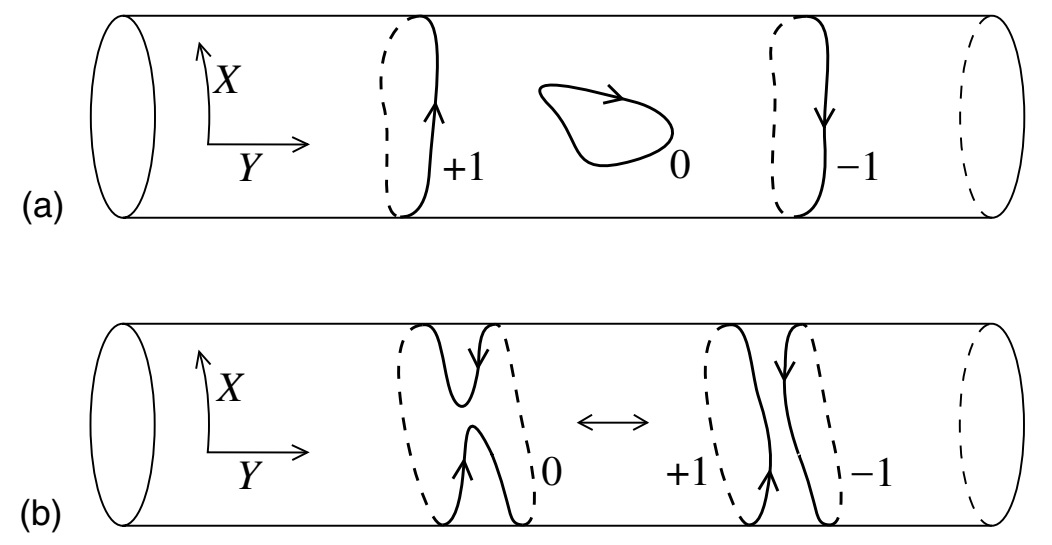
\includegraphics[width=0.8\textwidth]{figure/Fig8.1.jpg}
		\caption{(a) Oriented closed strings with winding numbers $w=+1,0,-1$.
			(b) Transition of a $w=0$ string into $w=+1$ and $w=-1$ strings.}\label{Fig8.1}
	\end{center}
\end{figure}

The second effect is unique to string theory. Closed strings can now wind around the compact dimension:
\begin{equation}
	X(\sigma+2 \pi)=X(\sigma)+2 \pi R w, \quad w \in \mathds{Z} \:. \label{8.2.3}
\end{equation}
The integer $w$ is the winding number.
States with winding numbers $+1, 0, -1$ are shown in Figure \ref{Fig8.1}(a).
From the viewpoint of worldsheet field theory, strings with non-zero winding number are topological solitons, i.e., states with topologically non-trivial field configurations. Consistent string theory must incorporate winding number states: through split-merge processes, 
$w=0$ strings can become $w=+1$ and $w=-1$ strings, as shown in Figure \ref{Fig8.1}(b). It is easy to see that winding number is always conserved in this example.
To determine the states of the closed string CFT, examine the Laurent expansion:
\begin{equation}
	\partial X(z)=-\mi\left(\frac{\alpha^{\prime}}{2}\right)^{1 / 2} \sum_{m=-\infty}^{\infty} \frac{\alpha_{m}}{z^{m+1}}\:, \qquad 
	\bar{\partial} X(\bar{z})=-\mi\left(\frac{\alpha^{\prime}}{2}\right)^{1 / 2} \sum_{m=-\infty}^{\infty} \frac{\tilde{\alpha}_{m}}{\bar{z}^{m+1}} \:. \label{8.2.4}
\end{equation}
After winding once, the change in $X$ is:
\begin{equation}
	2 \pi R w=\oint(\dif z\: \partial X + \dif \bar{z}\: \bar{\partial} X)= 2 \pi(\alpha^{\prime}/2)^{1/2}(\alpha_{0}-\tilde{\alpha}_{0}) \:. \label{8.2.5}
\end{equation}
The total Noether momentum is:
\begin{equation}
	p=\frac{1}{2 \pi \alpha^{\prime}} \oint(\dif z\: \partial X- \dif \bar{z}\: \bar{\partial} X)
	=(2 \alpha^{\prime})^{-1 / 2}(\alpha_{0}+\tilde{\alpha}_{0}) \:. \label{8.2.6}
\end{equation}
For non-compact dimensions, this gives $\alpha_{0}=\tilde{\alpha}_{0}=p(\alpha^{\prime} / 2)^{1 / 2}$ as usual, but for periodic dimensions we have:
\begin{subequations} \label{8.2.7}
	\begin{align}
		p_{L} \equiv\left(2 / \alpha^{\prime}\right)^{1 / 2} \alpha_{0}=\frac{n}{R}+\frac{w R}{\alpha^{\prime}} \:, \label{8.2.7a} \\
		p_{R} \equiv\left(2 / \alpha^{\prime}\right)^{1 / 2} \tilde{\alpha}_{0}=\frac{n}{R}-\frac{w R}{\alpha^{\prime}} \:. \label{8.2.7b}
	\end{align}		
\end{subequations}
The Virasoro generators are:
\begin{subequations} \label{8.2.8}
	\begin{align}
		L_{0}&=\frac{\alpha^{\prime} p_{L}^{2}}{4}+\sum_{n=1}^{\infty} \alpha_{-n} \alpha_{n} \:, \label{8.2.8a} \\
		\tilde{L}_{0}&=\frac{\alpha^{\prime} p_{R}^{2}}{4}+\sum_{n=1}^{\infty} \tilde{\alpha}_{-n} \tilde{\alpha}_{n} \:. \label{8.2.8b}
	\end{align}		 				
\end{subequations}

\subsection*{Partition Function}
The partition function for $X$ is:
\begin{align}
	&(q \bar{q})^{-1 / 24} \operatorname{Tr}\Bigl(q^{L_{0}} \bar{q}^{\tilde{L}_{0}}\Bigr) \nonumber \\
	&\quad =|\eta(\tau)|^{-2} \sum_{n, w=-\infty}^{\infty} q^{\alpha^{\prime} p_{L}^{2} / 4} \bar{q}^{\alpha^{\prime} p_{R}^{2} / 4} \nonumber \\
	&\quad =|\eta(\tau)|^{-2} \sum_{n, w=-\infty}^{\infty} \exp \left[-\pi \tau_{2}\left(\frac{\alpha^{\prime} n^{2}}{R^{2}}+\frac{w^{2} R^{2}}{\alpha^{\prime}}\right)+2 \pi \mi \tau_{1} n w\right] \:. \label{8.2.9}
\end{align}
The oscillators are the same as in the non-compact case, while the momentum integral is replaced by a sum over $n$ and $w$. Modular invariance is not obvious, but using the Poisson resummation formula:
\begin{equation}
	\sum_{n=-\infty}^{\infty} \exp (-\pi a n^{2}+2 \pi \mi b n)=a^{-1 / 2} 
	\sum_{m=-\infty}^{\infty} \exp \biggl[-\frac{\pi(m-b)^{2}}{a}\biggr] \:. \label{8.2.10}
\end{equation}
\begin{tcolorbox}[breakable]
	\begin{proof}
		Poisson resummation formula relates:
		\begin{align*}
			\sum_{n=-\infty}^{\infty} f(n) = \sum_{k=-\infty}^{\infty} \hat{f}(k) \tag{8.88}
		\end{align*}		
		where \(\hat{f}(k) = \int_{-\infty}^{\infty} dx \, e^{-2\pi i x k} f(x)\) is the Fourier transform of \(f(x)\). In our case we have
		\begin{align*}
			\hat{f}(k) &= \int_{-\infty}^{\infty} dx \, e^{-2\pi i x k} e^{-\pi a x^2 + 2\pi ibx} \\
			&= \int_{-\infty}^{\infty} dx \, e^{-\pi a x^2 + 2\pi i (b-k)x} \\
			&= \sqrt{\frac{\pi}{\pi a}} \, e^{\frac{-4\pi^2 (b-k)^2}{4\pi a}} \\
			&= a^{-1/2} e^{\frac{-\pi (b-k)^2}{a}} \tag{8.89}
		\end{align*}
		where we have used the Gaussian integral
		\begin{align*}
			\int_{-\infty}^{\infty} dx \, e^{-\alpha x^2 + \beta x} = \sqrt{\frac{\pi}{\alpha}} \, e^{\frac{\beta^2}{4\alpha}}
		\end{align*}
		Thus
		\begin{align*}
			\sum_{n=-\infty}^{\infty} \exp\left(-\pi a n^2 + 2\pi i b n\right) 
			= a^{-1/2} \sum_{m=-\infty}^{\infty} \exp\left[-\frac{\pi (m-b)^2}{a}\right]
		\end{align*}
	\end{proof}
\end{tcolorbox}
The partition function becomes:
\begin{equation}
	2 \pi R Z_{X}(\tau) \sum_{m, w=-\infty}^{\infty} \exp \biggl(-\frac{\pi R^{2}|m-w \tau|^{2}}{\alpha^{\prime} \tau_{2}}\biggr) \:. \label{8.2.11}
\end{equation}
$Z_{X}(\tau)$ is the modular invariant expression \eqref{7.2.9} for the non-compact theory; this sum is clearly invariant under $\tau \rightarrow \tau+1$. Under $\tau \rightarrow-1 / \tau$, it is invariant under $m\to-w$ and $w\to m$.

\begin{tcolorbox}[breakable]
	\begin{proof}
	The Poisson summation formula with \( a = \alpha' \tau_2 / R^2 \) and \( b = w \tau_1 \) on \eqref{8.2.9} becomes:
	\begin{align*}
		(q\bar{q})^{-1/24} \text{Tr } q^{L_0} \bar{q}^{\tilde{L}_0} 
		&= |\eta(\tau)|^{-2} \sum_{w=-\infty}^{\infty} \exp\left(-\frac{\pi \tau_2 R^2 w^2}{\alpha'} \right) \\
		&\quad \times \left( \frac{\alpha' \tau_2}{R^2} \right)^{-1/2} \sum_{m=-\infty}^{\infty} \exp\left[-\frac{\pi(m - w \tau_1)^2}{\alpha' \tau_2 / R^2}\right] \\
		&= |\eta(\tau)|^{-2} \frac{R}{(\alpha' \tau_2)^{1/2}} \sum_{m,w=-\infty}^{\infty} e^{-\frac{\pi R^2}{\alpha' \tau_2} \left[\tau_2^2 w^2 + (m-w \tau_1)^2\right]} \\
		&= |\eta(\tau)|^{-2} \frac{R}{(\alpha' \tau_2)^{1/2}} \sum_{m,w=-\infty}^{\infty} e^{-\frac{\pi R^2}{\alpha' \tau_2} \left[w^2 (\tau_1^2 + \tau_2^2) + m^2 - 2mw \tau_1\right]} 
	\end{align*}	
	Note now that
	\begin{align*}
		|m - w \tau|^2 &= (m - w \tau)(m - w \bar{\tau}) \\
		&= m^2 + w^2 |\tau|^2 - m w (\tau + \bar{\tau}) \\
		&= m^2 + w^2 (\tau_1^2 + \tau_2^2) - 2m w \tau_1 
	\end{align*}	
	and thus
	\begin{align*}
		(q\bar{q})^{-1/24} \text{Tr } q^{L_0} \bar{q}^{\tilde{L}_0} 
		= |\eta(\tau)|^{-2} \frac{R}{(\alpha' \tau_2)^{1/2}} \sum_{m,w=-\infty}^{\infty} e^{-\frac{\pi R^2 |m-w \tau|^2}{\alpha' \tau_2}} 
	\end{align*}
	We use \eqref{7.2.9}, i.e. \(|\eta(\tau)|^{-2} = (4\pi^2 \alpha' \tau_2)^{1/2} Z_X(\tau)\) to find
	\begin{align*}
		(q\bar{q})^{-1/24} \text{Tr } q^{L_0} \bar{q}^{\tilde{L}_0} 
		&= (4\pi^2 \alpha' \tau_2)^{1/2} Z_X(\tau) \frac{R}{(\alpha' \tau_2)^{1/2}} \sum_{m,w=-\infty}^{\infty} e^{-\frac{\pi R^2 |m-w \tau|^2}{\alpha' \tau_2}} \\
		&= 2\pi R Z_X(\tau) \sum_{m,w=-\infty}^{\infty} e^{-\frac{\pi R^2 |m-w \tau|^2}{\alpha' \tau_2}} 
	\end{align*}	
	Under \( \tau \to -1/\tau \) we have \( \tau_1 \to -\tau_1/|\tau|^2 \) and \( \tau_2 \to \tau_2/|\tau|^2 \). Thus
	\begin{align*}
		\sum_{m,w} \exp\left(-\frac{\pi R^2}{\alpha'} \frac{|m-w\tau|^2}{\tau_2}\right) 
		&\to \sum_{m,w} \exp\left(-\frac{\pi R^2}{\alpha'} \frac{|m+w/\tau|^2}{\tau_2/|\tau|^2}\right) \\
		&= \sum_{m,w} \exp\left(-\frac{\pi R^2}{\alpha'} \frac{|m\tau+w|^2}{\tau_2}\right) \\
		&= \sum_{w,m} \exp\left(-\frac{\pi R^2}{\alpha'} \frac{|-w\tau+m|^2}{\tau_2}\right)
	\end{align*}
	In the last line we have set \( w' = -m \) and \( m' = w \).
	\end{proof}
\end{tcolorbox}

\eqref{8.2.11} has a simple path integral interpretation.
Summing over all genus 1 worldsheets in periodic spacetime, each non-trivial closed curve on the worldsheet winds around the compact direction:
\begin{subequations} \label{8.2.12}
	\begin{align}
		X(\sigma^{1}+2 \pi, \sigma^{2}) &= X(\sigma^{1}, \sigma^{2})+2 \pi w R \:, \label{8.2.12a} \\
		X(\sigma^{1}+2 \pi \tau_{1}, \sigma^{2}+2 \pi \tau_{2}) &= X(\sigma^{1}, \sigma^{2})+2 \pi m R \:. \label{8.2.12b} 
	\end{align}
\end{subequations}
That is, the path integral splits into topologically inequivalent sectors labeled by $w$ and $m$. By writing $X$ as a classical solution satisfying periodicity:
\begin{equation}
	X_{\mathrm{cl}}=\sigma^{1} w R+\sigma^{2}(m-w \tau_{1}) R / \tau_{2} \:, \label{8.2.13}
\end{equation}
plus a quantum part satisfying periodic boundary conditions.
This Gaussian path integral can be integrated out. The path integral for the quantum part is the same as in the non-compact case, while the classical part appears as the exponential in \eqref{8.2.11}. The effect of modular transformations on periodicity is simplified to swapping the summation variables $m$ and $w$.

\subsection*{Vertex Operators}
To construct winding states with $\alpha_{0} \neq \tilde{\alpha}_{0}$, we need independent variables $x_{L}$ and $x_{R}$ satisfying:
\begin{equation}
	[x_{L}, p_{L}]=[x_{R}, p_{R}]=\mi \:. \label{8.2.14}
\end{equation}
The field $X$ splits into holomorphic and anti-holomorphic parts:
\begin{equation}
	X(z, \bar{z})=X_{L}(z)+X_{R}(\bar{z}) \:, \label{8.2.15}
\end{equation}
where:
\begin{subequations} \label{8.2.16}
	\begin{align}
		X_{L}(z) &= x_{L}- \mi \frac{\alpha^{\prime}}{2} p_{L} \ln z+\mi\left(\frac{\alpha^{\prime}}{2}\right)^{1 / 2} 
		\sum_{m=-\infty \atop m \neq 0}^{\infty} \frac{\alpha_{m}}{m z^{m}} \:, \label{8.2.16a} \\
		X_{R}(\bar{z})&= x_{R}-\mi \frac{\alpha^{\prime}}{2} p_{R} \ln \bar{z}+\mi\left(\frac{\alpha^{\prime}}{2}\right)^{1 / 2} 
		\sum_{m=-\infty \atop m \neq 0}^{\infty} \frac{\tilde{\alpha}_{m}}{m \bar{z}^{m}} \:. \label{8.2.16b}
	\end{align}
\end{subequations}
If we restrict to states with $k_{L}=k_{R}$ and only use operators constructed from $X_{L}(z)+X_{R}(\bar{z})$, this reduces to the CFT of non-compact dimensions. Note that $\ln|z|$ does not have any branch cut, however $\ln(z)$ does. As a result, $X^{\mu}$'s multivalued-ness is inherited by the mode decomposition.

We now discuss OPEs and vertex operators. The form of the vertex operator is easily guessed, since the usual $XX$ operator product $-(\alpha^{\prime} / 2) \ln (z_{12} \bar{z}_{12})$ can be split into holomorphic and anti-holomorphic functions, thus:
\begin{subequations} \label{8.2.17}
	\begin{align}
		X_{L}(z_{1}) X_{L}(z_{2}) &\sim-\frac{\alpha^{\prime}}{2} \ln z_{12}, \quad 
		X_{R}(\bar{z}_{1}) X_{R}(\bar{z}_{2}) \sim-\frac{\alpha^{\prime}}{2} \ln \bar{z}_{12}  \:,  \label{8.2.17a} \\
		X_{L}(z_{1}) X_{R}(\bar{z}_{2}) &\sim 0 \:. \label{8.2.17b}
	\end{align}		
\end{subequations}
The operator corresponding to the state $|0 ; k_{L}, k_{R}\rangle$ is:
\begin{equation}
	\mathscr{V}_{k_{L} k_{R}}(z, \bar{z}) = : \mathrel{e^{\mi k_{L} X_{L}(z)+ \mi k_{R} X_{R}(\bar{z})}}: \label{8.2.18}
\end{equation}
The OPE is:
\begin{equation}
	\mathscr{V}_{k_{L} k_{R}}(z_{1}, \bar{z}_{1}) \mathscr{V}_{k_{L}^{\prime} k_{R}^{\prime}}(z_{2}, \bar{z}_{2}) \sim 
	z_{12}^{\alpha^{\prime} k_{L} k_{L}^{\prime} / 2} \bar{z}_{12}^{\alpha^{\prime} k_{R} k_{R}^{\prime} / 2} 
	\mathscr{V}_{(k+k^{\prime})_{L}(k+k^{\prime})_{R}}(z_{2}, \bar{z}_{2}) \:. \label{8.2.19}
\end{equation}
We will encounter branch points and cuts in various expressions; this is not surprising, as the field \textbf{$X$ is no longer single-valued} as the boundary condition being imposed \eqref{8.2.3} has changed. However, it is important that the OPE of the entire vertex operator must be single-valued: when $z_{1}$ winds around $z_{2}$ once, the net phase is 1.
\begin{equation}
	\exp [\pi \mi \alpha^{\prime}(k_{L} k_{L}^{\prime}-k_{R} k_{R}^{\prime})]
	=\exp [2 \pi \mi(n w^{\prime}+w n^{\prime})]=1 \:. \label{8.2.20}
\end{equation}
This is exactly what is necessary for the string amplitude to be well-defined.

\subsection*{A Trick}

The previous discussion is clearly correct, but we have been too casual about the handling of branch points and cuts in the logarithms.
If we swap $z_{1}$ and $z_{2}$, and the momenta $k$ and $k^{\prime} $, a problem arises in OPE \eqref{8.2.19}. The left side is symmetric, but the right side will differ by $\exp[\pi \mi(n w^{\prime}+w n^{\prime})]$.
Therefore, if $n w^{\prime}+w n^{\prime}$ is odd, there will be a negative sign difference. We can also see this problem in the following way. From the mode expansion, we can derive the equal-time $(|z_{1}|=|z_{2}|)$ commutator:
\begin{equation}
	[X_{L}(z_{1}), X_{L}(z_{2})]=\frac{\pi \mi \alpha^{\prime}}{2} \operatorname{sign}(\sigma_{1}^{1}-\sigma_{2}^{1}) \:. \label{8.2.21}
\end{equation}
\begin{tcolorbox}[breakable]
	\begin{proof}
		We chose the worldsheet coordinate \( \sigma^1 \) to be in the range \([-\pi, \pi]\); it still has periodicity \( 2\pi \). Defining as usual \( z = e^{-iw} = e^{-i\sigma^1 + \sigma^2} \) we thus have \( \ln z = -i\sigma^1 + \sigma^2 \) and thus \( \sigma^1 = -\Im \ln z \). The logarithm has a branch cut that we put on the negative real axis. Working out \([X_L(z_1), X_L(z_2)]\), the only non-zero commutation relations we have are \([x_L, p_L] = i\) and \([\alpha_m, \alpha_n] = m\delta_{m+n}\). Thus
		
		\begin{align*}
			[X_L(z_1), X_L(z_2)] &= \left[ x_L - i \frac{\alpha'}{2} p_L \ln z_1 + i \sqrt{\frac{\alpha'}{2}} \sum_{m \neq 0} \frac{\alpha_m}{mz_1^m},\right. \\
			&\qquad \left. x_L - i \frac{\alpha'}{2} p_L \ln z_2 + i \sqrt{\frac{\alpha'}{2}} \sum_{n \neq 0} \frac{\alpha_n}{nz_2^n} \right] \\
			&= -i \frac{\alpha'}{2} \ln z_2 [x_L, p_L] - i \frac{\alpha'}{2} \ln z_1 [p_L, x_L] - \frac{\alpha'}{2} \sum_{m,n \neq 0} \frac{[\alpha_m, \alpha_n]}{mnz_1^m z_2^n} \\
			&= \frac{\alpha'}{2} \left( \ln z_2 - \ln z_1 - \sum_{m,n \neq 0} \frac{m\delta_{m+n}}{mnz_1^m z_2^n} \right) \\
			&= \frac{\alpha'}{2} \left( \ln z_2 - \ln z_1 - \sum_{n \neq 0} \frac{z_1^n}{nz_2^n} \right)
		\end{align*}
		
		Now from \(\ln(1-x) = -\sum_{n=1}^\infty x^n / n\) we have
		
		\begin{align*}
			\ln \left( 1 - \frac{z_1}{z_2} \right) - \ln \left( 1 - \frac{z_2}{z_1} \right) &= -\sum_{n=1}^\infty \frac{z_1^n}{nz_2^n} + \sum_{n=1}^\infty \frac{z_2^n}{nz_1^n} \\
			&= -\sum_{n=1}^\infty \frac{z_1^n}{nz_2^n} - \sum_{m=-\infty}^{-1} \frac{z_1^m}{mz_2^m} \\
			&= -\sum_{n \neq 0} \frac{z_1^n}{nz_2^n}
		\end{align*}
		
		and thus
		
		\begin{align*}
			[X_L(z_1), X_L(z_2)] &= \frac{\alpha'}{2} \left[ \ln z_2 - \ln z_1 + \ln \left( 1 - \frac{z_1}{z_2} \right) - \ln \left( 1 - \frac{z_2}{z_1} \right) \right] \\
			&= \frac{\alpha'}{2} \left[ \ln z_2 - \ln z_1 + \ln \frac{(z_2 - z_1)/z_2}{(z_1 - z_2)/z_1} \right] \\
			&= \frac{\alpha'}{2} \left[ \ln z_2 - \ln z_1 + \ln \left( -\frac{z_1}{z_2} \right) \right]
		\end{align*}
		Using \( z = e^{-i\sigma^1 + \sigma^2} \) and the fact that we have equal time commutators, i.e. that \( \sigma_1^2 = \sigma_2^2 \) we have
		
		\begin{align*}
			[X_L(z_1), X_L(z_2)] &= \frac{\alpha'}{2} \left[ -i\sigma_2^1 +\cancel{ \sigma_2^2} + i\sigma_1^1 -\cancel{ \sigma_1^2}+ \ln \left( e^{\pm i\pi} \frac{e^{-i\sigma_1^1 + \cancel{\sigma_1^2}}}{e^{-i\sigma_2^1 + \cancel{\sigma_2^2}}} \right) \right] \\
			&= \frac{\alpha'}{2} \left( -i\sigma_2^1 + i\sigma_1^1 + \ln e^{\pm i\pi - i\sigma_1^1 + i\sigma_2^1} \right) \\
			&= i\frac{\alpha'}{2} \left( -\sigma^1_2 + \sigma_1^1 \pm \pi - \sigma_1^1 + \sigma^1_2 \right) = \pm \frac{\pi i\alpha'}{2}
		\end{align*}
		Let us examine the logarithm in more detail: \(\ln e^{i(\pm\pi - \sigma_1^1 + \sigma_2^1)}\). If \(\sigma_1^1 > \sigma_2^1\), then \(-\sigma_1^1 + \sigma_2^1 < 0\). In this case we need to take the \(+\) sign. The most negative extreme occurs when \(\sigma_1^1 = +\pi\) and \(\sigma_2^1 = -\pi\), giving \(-\sigma_1^1 + \sigma_2^1 = -2\pi\). This value lies on the branch cut of logarithm; we can bring it back into the range \([-\pi, \pi]\) by adding \(+\pi\).
		
		Conversely, if \(\sigma_1^1 < \sigma_2^1\), then \(-\sigma_1^1 + \sigma_2^1 > 0\). Here we need to take the \(-\) sign. The most positive extreme occurs when \(\sigma_1^1 = -\pi\) and \(\sigma_2^1 = +\pi\), giving \(-\sigma_1^1 + \sigma_2^1 = 2\pi\). This also lies on the branch cut; we can bring it back into the range \([-\pi, \pi]\) by subtracting \(\pi\).
		
		We thus conclude that, indeed,
		\begin{align*}
			[X_L(z_1), X_L(z_2)] = \frac{\pi i\alpha'}{2} \operatorname{sign}(\sigma_1^1 - \sigma_2^1)
		\end{align*}
		We now use \(\bar{z} = e^{+i\sigma^1 + \sigma^2}\) and the fact that we have equal time commutators, to find
		
		\begin{align*}
			[X_R(z_1), X_R(z_2)] &= \frac{\alpha'}{2} \left[ i\sigma_2^1 + \sigma_2^2 - i\sigma_1^1 - \sigma_1^2 + \ln \left( e^{\pm i\pi} \frac{e^{+i\sigma_1^1 + \sigma_1^2}}{e^{+i\sigma_2^1 + \sigma_2^2}} \right) \right] \\
			&= \frac{\alpha'}{2} \left( +i\sigma_2^1 - i\sigma_1^1 + \ln e^{\pm i\pi + i\sigma_1^1 - i\sigma^1_2} \right) = \pm \frac{\pi i\alpha'}{2}
		\end{align*}
		
		We work out the sign in the same way as before, but now as the argument of the logarithm is \(\ln e^{i(\pm\pi + \sigma_1^1 - \sigma_2^1)}\) and not \(\ln e^{i(\pm\pi - \sigma_1^1 + \sigma_2^1)}\) we have the rôle of \(\sigma_1^1\) and \(\sigma_2^1\) interchanged. Therefore
		
		\begin{align*}
			[X_R(z_1), X_R(z_2)] = -\frac{\pi i\alpha'}{2} \operatorname{sign}(\sigma_1^1 - \sigma_2^1)
		\end{align*}
		QED.
	\end{proof}
\end{tcolorbox}
The CBH formula then tells us that if we define the operator through a creation-annihilation order, then when $n w^{\prime}+w n^{\prime}$ is odd, the operator $\mathscr{V}_{k_{L} k_{R}}$ anticommutes with $\mathscr{V}_{k_{k}^{\prime} k_{R}^{\prime}}$. The invisible branch point/cut \eqref{8.2.20} becomes two visible ones.
The correct oscillator expression for the vertex operator is (with some ambiguity in the phase):
\begin{equation}
	\mathscr{V}_{k_{L} k_{R}}(z, \bar{z})=\exp [\pi \mi(k_{L}-k_{R})(p_{L}+p_{R}) \alpha^{\prime} / 4] 
	\mathrel{\typecolon \me^{\mi k_{L} X_{L}(z)+\mi k_{R} X_{R}(\bar{z})} \typecolon} \:, \label{8.2.22}
\end{equation}
where $p_L, p_R$ are operators as usual, and $k$ is a number (the momentum carried by the given vertex operator).
When $\mathscr{V}_{k_{L} k_{R}}$ and $\mathscr{V}_{k_{L}^{\prime} k_{R}^{\prime}}$ commute with each other, the extra factor is called cocycles, which gives an extra phase:
\begin{align}
	\exp \Bigl\{\pi \mi\Bigl[(k_{L}-k_{R})(k_{L}^{\prime}+k_{R}^{\prime})-(k_{L}^{\prime}-k_{R}^{\prime})(k_{L}+k_{R})\Bigr] 
	\alpha^{\prime} / 4\Bigr\}\quad &  \nonumber \\
	=\exp [\pi \mi(n w^{\prime}-w n^{\prime})] &\:, \label{8.2.23}
\end{align}
which removes the branch points and cuts.
In most cases, this complexity can be ignored, and the simpler expression from the previous paragraph can be used; cocycles only affect the relative signs of specific amplitudes.
\begin{tcolorbox}[breakable]
	\begin{proof}
		\begin{align}
			\mathscr{V}_{k_{L_1}k_{R_1}}(z_1,\bar z_1)\mathscr{V}_{k_{L_2}k_{R_2}}(z_2,\bar z_2)
			&= e^{i\pi(k_{L_1}-k_{R_1})(p_L+p_R)\alpha'/4}e^{ik_{L_1}X_L(z_1)+ik_{R_1}X_R(\bar{z}_1)} \nonumber\\
			&\quad \times e^{i\pi(k_{L_2}-k_{R_2})(p_L+p_R)\alpha'/4}e^{ik_{L_2}X_L(z_2)+ik_{R_2}X_R(\bar{z}_2)}\label{8.117}
		\end{align}
		
		The \( p \) are momentum operators, so they pick up the momentum component of everything that is to their right. This thus becomes
		
		\begin{align}
			\mathscr{V}_{k_{L_1}k_{R_1}}(z_1,\bar z_1)\mathscr{V}_{k_{L_2}k_{R_2}}(z_2,\bar z_2)
			&= e^{i\pi(k_{L_1}-k_{R_1})(k_{L_1}+k_{L_2}+k_{R_1}+k_{R_2})\alpha'/4}e^{ik_{L_1}X_L(z_1)+ik_{R_1}X_R(\bar{z}_1)} \nonumber\\
			&\quad \times e^{i\pi(k_{L_2}-k_{R_2})(k_{L_2}+k_{R_2})\alpha'/4}e^{ik_{L_2}X_L(z_2)+ik_{R_2}X_R(\bar{z}_2)} \nonumber\\
			&= e^{i\pi\left[(k_{L_1}-k_{R_1})(k_{L_1}+k_{L_2}+k_{R_1}+k_{R_2})+(k_{L_2}-k_{R_2})(k_{L_2}+k_{R_2})\right]\alpha'/4} \nonumber\\
			&\quad \times e^{ik_{L_1}X_L(z_1)+ik_{R_1}X_R(\bar{z}_1)}e^{ik_{L_2}X_L(z_2)+ik_{R_2}X_R(\bar{z}_2)}
		\end{align}
		
		Using \eqref{8.117}
		
		\begin{align}
			\mathscr{V}_{k_{L_1}k_{R_1}}(z_1,\bar z_1)\mathscr{V}_{k_{L_2}k_{R_2}}(z_2,\bar z_2)
			&= e^{i\pi\left[(k_{L_1}-k_{R_1})(k_{L_1}+k_{L_2}+k_{R_1}+k_{R_2})+(k_{L_2}-k_{R_2})(k_{L_2}+k_{R_2})\right]\alpha'/4} \nonumber\\
			&\quad \times (-)^{n_1w_2+w_1n_2}e^{ik_{L_2}X_L(z_2)+ik_{R_2}X_R(\bar{z}_2)}e^{ik_{L_1}X_L(z_1)+ik_{R_1}X_R(\bar{z}_1)} 
		\end{align}
		
		and re-introduce the cocycles and their inverse. This gives
		
		\begin{align}
			\mathscr{V}_{k_{L_1}k_{R_1}}(z_1,\bar z_1)\mathscr{V}_{k_{L_2}k_{R_2}}(z_2,\bar z_2)
			&= e^{i\pi\left[(k_{L_1}-k_{R_1})(k_{L_1}+k_{L_2}+k_{R_1}+k_{R_2})+(k_{L_2}-k_{R_2})(k_{L_2}+k_{R_2})\right]\alpha'/4} \nonumber\\
			&\quad \times (-)^{n_1w_2+w_1n_2}e^{-i\pi(k_{L_2}-k_{R_2})(k_{L_1}+k_{L_2}+k_{R_1}+k_{R_2})} \nonumber\\
			&\quad \times e^{-i\pi(k_{L_1}-k_{R_1})(k_{L_1}+k_{R_1})\alpha'/4}\,
			\mathscr{V}_{k_{L_2}k_{R_2}}(z_2,\bar z_2)\mathscr{V}_{k_{L_1}k_{R_1}}(z_1,\bar z_1) 
		\end{align}
		
		It remains to work out the phase:
		
		\begin{align}
			\mathscr{V}_{k_{L_1}k_{R_1}}(z_1,\bar z_1)\mathscr{V}_{k_{L_2}k_{R_2}}(z_2,\bar z_2)
			&= (-)^{n_1w_2+w_1n_2}e^{i\pi\left[(k_{L_1}-k_{R_1})(k_{L_2}+k_{R_2})-(k_{L_2}-k_{R_2})(k_{L_1}+k_{R_1})\right]\alpha'/4} \nonumber\\
			&\quad \times \mathscr{V}_{k_{L_2}k_{R_2}}(z_2,\bar z_2)\mathscr{V}_{k_{L_1}k_{R_1}}(z_1,\bar z_1) \nonumber\\
			&= (-)^{n_1w_2+w_1n_2}e^{i\pi(2k_{L_1}k_{R_2}-2k_{R_1}k_{L_2})\alpha'/4}\notag\\
			&\qquad\times\mathscr{V}_{k_{L_2}k_{R_2}}(z_2,\bar z_2)\mathscr{V}_{k_{L_1}k_{R_1}}(z_1,\bar z_1) 
		\end{align}
		
		We find
		
		\begin{align}
			k_{L_1}k_{R_2} - k_{R_1}k_{L_2}
			&= \left( \frac{n_1}{R} + \frac{w_1R}{\alpha'} \right) \left( \frac{n_2}{R} - \frac{w_2R}{\alpha'} \right) - \left( \frac{n_1}{R} - \frac{w_1R}{\alpha'} \right) \left( \frac{n_2}{R} + \frac{w_2R}{\alpha'} \right) \nonumber\\
			&= -2 \frac{n_1w_2 - w_1n_2}{\alpha'}
		\end{align}
		
		and thus
		
		\begin{align}
			\mathscr{V}_{k_{L_1}k_{R_1}}(z_1,\bar z_1)\mathscr{V}_{k_{L_2}k_{R_2}}(z_2,\bar z_2)
			&= (-)^{n_1w_2 + w_1n_2}e^{-i\pi(n_1w_2 - w_1n_2)}\,
			\mathscr{V}_{k_{L_2}k_{R_2}}(z_2,\bar z_2)\mathscr{V}_{k_{L_1}k_{R_1}}(z_1,\bar z_1) \nonumber\\
			&= (-)^{n_1w_2 + w_1n_2}(-)^{n_1w_2 - w_1n_2}\,
			\mathscr{V}_{k_{L_2}k_{R_2}}(z_2,\bar z_2)\mathscr{V}_{k_{L_1}k_{R_1}}(z_1,\bar z_1) \nonumber\\
			&= (-)^{2n_1w_2}\,
			\mathscr{V}_{k_{L_2}k_{R_2}}(z_2,\bar z_2)\mathscr{V}_{k_{L_1}k_{R_1}}(z_1,\bar z_1) \nonumber\\
			&= \mathscr{V}_{k_{L_2}k_{R_2}}(z_2,\bar z_2)\mathscr{V}_{k_{L_1}k_{R_1}}(z_1,\bar z_1)
		\end{align}
		
		as \( 2n_1w_2 \) is always even. We thus see that adding the cocycle indeed ensures that the vertex operators commute.
	\end{proof}
\end{tcolorbox}
The general $X^{\mu}$ path integral \eqref{6.2.18} factors into holomorphic and anti-holomorphic parts in an obvious way, allowing for the substitution:
\begin{equation}
	\prod_{i<j}^{n}|z_{i j}|^{\alpha^{\prime} k_{i} k_{j}} \to \prod_{i<j}^{n} z_{i j}^{\alpha^{\prime} k_{L i} k_{L j} / 2} 
	\bar{z}_{i j}^{\alpha^{\prime} k_{R i} k_{R j} / 2} \:, \label{8.2.24}
\end{equation}
and we can also replace the $2 \pi \delta(\sum k)$ from the non-compact integral over $x_{0}$ with:
\begin{equation}
	2 \pi R \delta_{\Sigma_{i} n_{i}, 0} \delta_{\Sigma_{i} w_{i}, 0} \:. \label{8.2.25}
\end{equation}
The exact expression \eqref{8.2.22} will yield some additional signs.

\subsection*{DDF Operators}

We have seen that exponential operators can be split into holomorphic and anti-holomorphic parts, which has many applications. We now use this to discuss the DDF operators mentioned at the end of Chapter 4.

We will work with light-cone coordinates $X^{\pm}=2^{-1 / 2}(X^{0} \pm X^{1})$, whose holomorphic part has the OPE (dropping the $L$ subscript):
\begin{equation}
	X^{+}(z) X^{-}(0) \sim \frac{\alpha^{\prime}}{2} \ln z, \qquad X^{+}(z) X^{+}(0) \sim X^{-}(z) X^{-}(0) \sim 0 \:. \label{8.2.26}
\end{equation}
\begin{tcolorbox}
	\begin{remark}
		\begin{align}
			X^{+}(z) X^{-}(0) &= 2^{-1}\left(X^{0}(z)+X^{\prime}(z)\right)\left(X^{0}(0)-X^{\prime}(0)\right) 
			= 2^{-1}\left(\frac{\alpha^{\prime}}{2} \ln z_{12}+\frac{\alpha^{\prime}}{2}\ln z_{12}\right)\notag\\
			&=\frac{\alpha^{\prime}}{2} \ln z_{12} \:. \label{8.2.27}
		\end{align}
	\end{remark}
\end{tcolorbox}
\noindent From this, it follows that the operator:
\begin{equation}
	V^{i}(n k_{0}, z)=\partial X^{i}(z) \me^{\mi n k_{0} X^{+}(z)}(2 / \alpha^{\prime})^{1 / 2} \label{8.2.28}
\end{equation}
is a $(1,0)$ primary field, where $i$ is a transverse index.
The OPE is:
\begin{align}
	V^{i}(n k_{0}, z) V^{j}(m k_{0}, 0) &\sim-\frac{\delta^{i j}}{z^{2}} \me^{\mi(n+m) k_{0} X^{+}(0)}  \nonumber \\
	&\quad -\frac{\mi n k_{0} \delta^{i j}}{z} \partial X^{+}(0) \me^{\mi(n+m) k_{0} X^{+}(0)} \:. \label{8.2.29}
\end{align}
Define the DDF operator as:
\begin{equation}
	A_{n}^{i}=\oint \frac{\dif z}{2 \pi} \, V^{i}(n k_{0}, z) \:. \label{8.2.30}
\end{equation}
Unless $n+m=0$, the $z^{-1}$ term in OPE \eqref{8.2.28} is a total derivative, so the DDF operators satisfy the oscillator algebra:
\begin{equation}
	[A_{m}^{i}, A_{n}^{j}]=m \delta^{i j} \delta_{m,-n} \frac{\alpha^{\prime} k_{0} p^{+}}{2} \:. \label{8.2.31}
\end{equation}

Examine the action of this operator on a state with given momentum $q$. The vertex operator for $V^{i}(n k_{0}, z)$ and this state will contain $z^{-\alpha^{\prime} n k_{0} q^{-} / 2}$. 
Thus, if we fix $k_{0}=2 / \alpha^{\prime} q^{-}$, it will be single-valued. Then the contour integral \eqref{8.2.29} defines a reasonable operator in this sector.
The DDF operator is the integral of a $(1,0)$ tensor and thus commutes with the Virasoro generators, transforming physical states into physical states. From this, we can build physical states by acting on the oscillator ground state with DDF operators. 
The states obtained in this way correspond one-to-one with light-cone states. DDF operators do not contain $X^{-}$, so these states have no $\alpha_{-m}^{-}$ excitations. 
Thus, compared to the more general but less obvious construction in \eqref{4.4.19}, they actually yield the same states.

\section{\texorpdfstring{Closed Strings and $T$-duality}{8.3 Closed Strings and $T$-duality}} \label{sec:8.3}

Since we are studying string theory, we take $D=26$ and only assume $X^{25}$ is periodic.
The mass shell ($L_{0}$ and $\tilde{L}_{0}$) is:
\begin{align}
	m^{2}=-k^{\mu} k_{\mu} &= (k_{L}^{25})^{2}+\frac{4}{\alpha^{\prime}}(N-1) \nonumber \\
	&=(k_{R}^{25})^{2}+\frac{4}{\alpha^{\prime}}(\tilde{N}-1) \:, \label{8.3.1}
\end{align}
or:
\begin{subequations} \label{8.3.2}
	\begin{align}
		m^{2} &= \frac{n^{2}}{R^{2}}+\frac{w^{2} R^{2}}{\alpha^{\prime 2}}+\frac{2}{\alpha^{\prime}}(N+\tilde{N}-2) \:, \label{8.3.2a} \\
		0 &= n w+N-\tilde{N} \:. \label{8.3.2b} 
	\end{align}
\end{subequations}
There are four contributions to mass squared: compact momentum, winding string potential energy, oscillators, and zero-point energy. The discussion of the physical spectrum in Chapter 4 applies to any compactification, 
so we obtain the correct counting of states just by examining the transverse oscillators $M=2, \ldots, 25$.

First, we reproduce the field theory result for the massless spectrum. At a general value of $R$, states can only be massless when $n=w=0$ and $N=\tilde{N}=1$.
There are $24^{2}$ identical states, but it is useful to classify them based on whether the oscillators are in the spacetime direction $\mu$ or the internal direction 25:
\begin{align}
	&\alpha_{-1}^{\mu} \tilde{\alpha}_{-1}^{\nu}|0 ; k\rangle\:, \qquad 
	(\alpha_{-1}^{\mu} \tilde{\alpha}_{-1}^{25}+\alpha_{-1}^{25} \tilde{\alpha}_{-1}^{\mu})|0 ; k\rangle \:, \nonumber \\
	&(\alpha_{-1}^{\mu} \tilde{\alpha}_{-1}^{25}-\alpha_{-1}^{25} \tilde{\alpha}_{-1}^{\mu})|0 ; k\rangle\:, \qquad 
	\alpha_{-1}^{25} \tilde{\alpha}_{-1}^{25}|0 ; k\rangle \:. \label{8.3.3}
\end{align}
The first set further splits into the 25-dimensional graviton plus dilaton plus antisymmetric tensor. The second is the graviton on spacetime and internal indices, which is the Kaluza-Klein vector. The third is the vector from the antisymmetric tensor.
The last state is a scalar, which is the modulus of the radius in the compact direction; its vertex operator $:\mathrel{\partial X^{25} \bar{\partial} X^{25} \me^{\mi k \cdot X}}:$ is a perturbation of the metric $G_{25,25}$. This is the same spectrum found when examining low-energy field theory.

Examining the transformation of massive states under $U(1) \times U(1)$ symmetry is very beneficial.
Once again, Kaluza-Klein gauge symmetry comes from translations in the $X^{25}$ direction, 
so the corresponding charge is the compact momentum $p_{25} $. For antisymmetric tensor gauge symmetry, examine the zero-momentum vertex operator, which measures the transformation of any state coupled to it.
It is proportional to:
\begin{equation}
	\partial X^{\mu} \bar{\partial} X^{25}-\partial X^{25} \bar{\partial} X^{\mu}= 
	\bar{\partial}(X^{25} \partial X^{\mu})-\partial(X^{25} \bar{\partial} X^{\mu}) \:. \label{8.3.4}
\end{equation}
This is a total derivative, but on winding states, its integral is non-zero since $X^{25}$ is not single-valued. So the $B_{\mu, 25}$ charge is the winding number.
This is the first "stringy" physics we encounter in this compactification: no state carries this charge in field theory.

We verify the gauge coupling from the string three-point coupling. The gauge boson vertex operator is:
\begin{equation}
	\frac{2^{1 / 2} g_{\mathrm{c}, 25}}{\alpha^{\prime}}:\mathrel{(\partial X^{\mu} \bar{\partial} X^{25} \pm 
		\partial X^{25} \bar{\partial} X^{\mu}) \me^{\mi k \cdot X}}: \:. \label{8.3.5}
\end{equation}
We set the 25-dimensional string coupling $g_{\mathrm{c}, 25}=g_{\mathrm{c}}(2 \pi R)^{-1 / 2}$. The factor $(2 \pi R)^{-1 / 2}$ comes from the normalization of the zero-mode wave function. 
For general compact momentum and winding number, the tachyon vertex operator is:
\begin{equation}
	g_{\mathrm{c}, 25}:\mathrel{ \me^{\mi k_{L} \cdot X_{L}(z)+\mi k_{R} \cdot X_{R}(\bar{z})}}: \:. \label{8.3.6}
\end{equation}
The three-point amplitude for one gauge boson and two tachyons, if the compact momentum and winding number of the tachyons are non-zero, is similar to \eqref{6.6.14}:
\begin{align}
	& {-}2^{-1 / 2} \pi \mi g_{\mathrm{c}, 25}(2 \pi)^{25} \delta^{25}({\textstyle\sum_{i} k_{i}}) k_{23}^{\mu}
	(k_{L 23}^{25} \pm k_{R 23}^{25}) \nonumber \\
	\to & {-}2^{3 / 2} \pi \mi g_{\mathrm{c}, 25}(2 \pi)^{25} \delta^{25}({\textstyle \sum_{i} k_{i}}) k_{2}^{\mu}
	(k_{L 2}^{25} \pm k_{R 2}^{25}) \:. \label{8.3.7}
\end{align}
In the second line, we take the gauge boson momentum $k_{1} \rightarrow 0$, which defines the gauge coupling. Two gauge bosons couple to $k_{L 2}^{25} \pm k_{R 2}^{25}$ respectively, i.e., compact momentum and winding number. 
This is exactly what we expect. Replacing the gauge boson with a graviton and continuing to examine this amplitude, we reproduce the relationships between couplings in \eqref{8.1.11} and \eqref{8.1.12}, which are the same as those found in the effective action.

\subsection*{Enhanced Gauge Symmetry}

Thus far, everything is identical to field theory with one compact dimension. The 26-dimensional graviton yields the 25-dimensional graviton plus vector plus modulus. The only string effect is the winding state carrying the $B_{\mu, 25}$ charge.

Further and more magical effects come from special compact radii. We omitted the discussion of the massless spectrum previously; states are only massless at special values of the radius $R$.
The most enriched case is $R=\alpha^{1 / 2}$, 
so $k_{L, R}^{25}=(n \pm w) \alpha^{\prime-1 / 2}$, and the condition for massless states is:
\begin{equation}
	(n+w)^{2}+4 N=(n-w)^{2}+4 \tilde{N}=4 \:. \label{8.3.8}
\end{equation}
Besides the general solution $n=w=0, N=\tilde{N}=1$, we now have:
\begin{equation}
	n=w=\pm 1,\: N=0,\: \tilde{N}=1\:, \quad n=-w=\pm 1, \: N=1, \:\tilde{N}=0 \:, \label{8.3.9}
\end{equation}
as well as:
\begin{equation}
	n=\pm 2,\: w=N=\tilde{N}=0\:, \quad w=\pm 2, \: n=N=\tilde{N}=0 \:. \label{8.3.10}
\end{equation}

States in \eqref{8.3.9} introduce four gauge bosons, with vertex operators:
\begin{equation}
	: \mathrel{\bar{\partial} X^{\mu} \me^{\mi k \cdot X} \exp [\pm 2 \mi \alpha^{\prime-1 / 2} X_{L}^{25}]}: \:, \quad 
	: \mathrel{ \partial X^{\mu} \me^{\mi k \cdot X} \exp [\pm 2 \mi \alpha^{\prime-1 / 2} X_{R}^{25}]}: \:. \label{8.3.11}
\end{equation}
The exact definition of the exponential operator is the same as in the previous section. These states possess internal momentum and winding number, so they carry Kaluza-Klein charge and antisymmetric tensor gauge charge. The only consistent theory for charged massless vectors is a non-Abelian gauge theory, 
so the new gauge bosons must combine with the old gauge bosons to form a non-Abelian theory. It is now convenient to treat the previous vectors using $\partial X^{25} \bar{\partial} X^{\mu}$ and $\partial X^{\mu} \bar{\partial} X^{25}$. 
The first one couples to $k_{L}^{25}$; under this coupling, the first pair of states in \eqref{8.3.11} carries charge $\pm 1$, while the second pair is neutral. 
The second couples to $k_{R}^{25}$, and so on.
This indicates that the gauge group is $S U(2) \times S U(2)$; the three vectors containing $\bar{\partial} X^{\mu}$ constitute an $S U(2)$. 
The other three constitute another $S U(2)$.
To present this $S U(2) \times S U(2)$, define three $(1,0)$ currents:
\begin{subequations} \label{8.3.12}
	\begin{align}
		j^{1}(z)&=: \mathrel{\cos [2 \alpha^{-1 / 2} X_{L}^{25}(z)]}: \:, \label{8.3.12a}  \\
		j^{2}(z)&=:\mathrel{ \sin [2 \alpha^{\prime-1 / 2} X_{L}^{25}(z)]}: \:, \label{8.3.12b} \\
		j^{3}(z)&=\mi \partial X_{L}^{25}(z) / \alpha^{\prime 1 / 2} \:. \label{8.3.12c}
	\end{align}
\end{subequations}
They can be normalized such that the OPE is:
\begin{equation}
	j^{i}(z) j^{j}(0) \sim \frac{\delta^{i j}}{2 z^{2}}+ \mi \frac{\epsilon^{i j k}}{z} j^{k}(0) \:. \label{8.3.13}
\end{equation}
For $(0,1)$ currents $\tilde{\jmath}^{i} $, there are similar OPEs. 
The single-pole term implies the corresponding charges form an $SU(2)$ algebra. In fact, since these currents are holomorphic, there is an infinite-dimensional algebra formed by Laurent coefficients:
\begin{subequations} \label{8.3.14}
	\begin{align}
		j^{i}(z) &= \sum_{m=-\infty}^{\infty} \frac{j_{m}^{i}}{z^{m+1}}  \:, \label{8.3.14a} \\
		[j_{m}^{i}, j_{n}^{j}] &= \frac{m}{2} \delta_{m,-n} \delta^{i j}+ \mi \epsilon^{i j k} j_{m+n}^{k} \:, \label{8.3.14b} 
	\end{align}
\end{subequations}
which is called a current algebra, affine Lie algebra, or Kac-Moody algebra.
We will encounter such algebras frequently at the beginning of Chapter 11. It will be proven that the coefficient of $z^{-2}$ is quantized, 
and the value in \eqref{8.3.13} is the minimum. So this is called a level 1 $SU(2)$ current algebra.

This $S U(2) \times S U(2)$ symmetry shows for the first time that string theory perceives spacetime geometry in a way that is completely different from what we use in field theory, 
where only $U(1) \times U(1)$ symmetry is obvious at any radius. 
The origins of $j^{3}$ and $j^{1,2}$ are completely different—they are oscillator excitations and winding number-momentum excitations, respectively, 
and their representations in terms of $X^{25}$ are also completely different, but in their action on the string spectrum, they are related to each other by symmetry. Since the energy of internal momentum and winding number is cancelled by negative zero-point energy, the extra vectors are massless. 
This situation occurs not only in tachyon theory, but also in other cases in Volume II.

\subsection*{Scale and Coupling}

At the $S U(2) \times S U(2)$ radius, the relation \eqref{8.1.11} becomes:
\footnote{More accurately, this is a coupling for an $(n, w)=(1,0)$ state. Non-Abelian gauge bosons have $(|n|,|w|)=(1,1)$, 
	so their coupling is $g_{S U(2), 25}^{2}=4 \kappa_{25}^{2} / \alpha^{\prime}$, which is the traditional quantum physics definition of $SU(2)$ coupling. 
	We will see in Chapter 18 that this holds for all level 1 current algebras.}
\begin{equation}
	g_{25}^{2}=2 \kappa_{25}^{2} / \alpha^{\prime} \:. \label{8.3.15}
\end{equation}
If we compactify multiple dimensions, each dimension scales the same way. So, specifically, in 4 dimensions:
\begin{equation}
	g_{4}^{2}=2 \kappa_{4}^{2} / \alpha^{\prime} \:. \label{8.3.16}
\end{equation}
In nature, non-Abelian gauge couplings are of order 1, which implies that the string length $\alpha^{1 / 2}$ is not far from the gravitational length $\kappa_{4}$.

We can also think of this in the following way. The 4-dimensional gauge coupling is dimensionless, but the 4-dimensional gravitational coupling has dimensions. Define an effective dimensionless gravitational coupling, which depends on the energy scale $E$:
\begin{equation}
	g_{\mathrm{G}, 4}^{2}(E)=\kappa_{4}^{2} E^{2} \:, \label{8.3.17}
\end{equation}
which grows with the square of energy. Obviously, the dimensionless gauge coupling runs with energy, but this is slower than the dimensional scaling of gravitational coupling. 
Then by \eqref{8.3.16}, the string mass scale is where the gauge and gravitational couplings are roughly equal, 
$g_{\mathrm{G}, 4}^{2}(E) \approx g_{4}^{2}$.

It is also beneficial to examine the possibility of compactification to 4 dimensions, where some compactification dimensions might be much larger than others. This is best analyzed by starting from low energy and working up, where a dimensionless gauge coupling $g_{4}^{2}$ exists at low energy. 
At energy $\rho_{5}^{-1}$, one compact dimension becomes a visible dimension, and physics becomes 5-dimensional (for simplicity, we only examine this one dimension at this scale).
The effective 5-dimensional coupling is:
\begin{equation}
	g_{5}^{2}=2 \pi \rho_{5} g_{4}^{2} \:. \label{8.3.18}
\end{equation}
Similar to \eqref{8.1.12}, this originates from the effective action. The coupling $g_{5}^{2}$ has dimensions of length. That is, 5-dimensional Yang-Mills theory, like 4-dimensional gravity, is non-renormalizable. 
Correspondingly, the effective dimensionless coupling is:
\begin{equation}
	\hat{g}_{5}^{2}=g_{5}^{2} E=2 \pi \rho_{5} E g_{4}^{2} \:, \label{8.3.19}
\end{equation}
which grows linearly with energy. However, $g_{4}^{2}$ is not much less than 1 in nature, so the coupling becomes strong quickly at high energy; it is presumed that string theory is then required to make the short-distance behavior reasonable. 
So this compactification scale must be close to the gravitational scale. This analysis is modified in open string theory, where modern understandings of strong-coupling string theory are taken into account. 
There is a very low probability that string or Kaluza-Klein excitations are far below the Planck scale.

\subsection*{Higgs Mechanism}
Let $R$ move away from the $S U(2) \times S U(2)$ radius. It is most instructive to examine what happens. The extra gauge bosons now acquire mass:
\begin{equation}
	m=\sqrt{\frac{R^4+\alpha{'}\,^2-2R^2\alpha'}{R^2\alpha'^2}}=\frac{|R^{2}-\alpha^{\prime}|}{R \alpha^{\prime}} \approx \frac{2}{\alpha^{\prime}}\Bigl|R-\alpha^{\prime 1 / 2}\Bigr| \:, \label{8.3.20}
\end{equation}
where the approximation holds when the radius $R$ is very close to the $S U(2) \times S U(2)$ radius $\alpha^{\prime 1 / 2}$. Near this radius, the mass is much smaller than the string scale, and we should use low-energy field theory to understand the physics.

There is only one way to endow gauge bosons with such mass: spontaneous symmetry breaking, which is exactly what occurs. 
When $R=\alpha^{1 / 2}$, there are 10 massless scalars: the dilaton, the modulus $G_{25,25}$, the four states in \eqref{8.3.9}, and the four states in \eqref{8.3.10}, the latter nine generated by the vertex operators:
\begin{equation}
	: \mathrel{j^{i}(z) \tilde{\jmath}^{j}(\bar{z}) \me^{\mi k \cdot X(z, \bar{z})}}: \:. \label{8.3.21}
\end{equation}
Index $i$ is a vector under the left-moving $SU(2)$, and index $j$ is a vector under the right-moving $SU(2)$. That is, they transform according to the $(\bm{3},\bm{3})$ representation under $S U(2) \times S U(2) $. 
In particular, the modulus of the radius is $j^{3} \tilde{\jmath}^{3}$. 
Moving away from the $S U(2) \times S U(2)$ radius gives this field an expectation value, 
so the gauge symmetry is broken down to the $U(1) \times U(1)$ symmetry that preserves the $z$-axis. Indeed, this is exactly the gauge group at a general radius. 
Near the $SU(2)$ radius, 
the mass \eqref{8.3.20} is linear with respect to the modulus dimension $|R-\alpha^{\prime 1 / 2}|$, just like standard spontaneous breaking. 

We denote the spacetime fields corresponding to these nine scalar fields as $M_{i j} $. 
One variation in the modulus is $M_{33} \neq 0$, but near the $S U(2) \times S U(2)$ point, it is very instructive to investigate more general backgrounds. The interactions of these massless fields will be described by some spacetime action, and this action will contain a potential $U(M)$. 
These fields have no mass at the symmetry point, so there is no $M^{2}$ term in $U$, 
but there may be $(S U(2) \times S U(2))$-invariant cubic terms:
\begin{equation}
	U(M) \propto \epsilon^{i j k} \epsilon^{i^{\prime} j^{\prime} k^{\prime}} M_{i i^{\prime}} M_{j j^{\prime}} M_{k k^{\prime}}=\operatorname{det} M \:. \label{8.3.22}
\end{equation}
It is not difficult to prove from the three-point string amplitude that this term indeed exists. It is a cubic term for bosons and is unbounded from below, but like the tachyon, this is an artifact of bosonic string theory.

Ignoring the fact that this potential is unstable for small variations, it is meaningful to find its static classical solutions. To have a static background solution, the field equations for the graviton and dilaton require the potential to be zero, and the field equations for $M_{i j}$ require the potential to be stable:
\begin{equation}
	U(M)=\frac{\partial U(M)}{\partial M_{i j}}=0 \:. \label{8.3.23}
\end{equation}
Diagonalizing $M$ using $S U(2) \times S U(2)$ rotations, the condition \eqref{8.3.23} becomes:
\begin{equation}
	M_{11} M_{22} M_{33}=M_{11} M_{22}=M_{11} M_{33}=M_{22} M_{33}=0 \:. \label{8.3.24}
\end{equation}
Therefore, only one diagonal component can be non-zero. 
By $S U(2) \times S U(2)$ rotations, we can take this non-zero diagonal component to be $M_{33} $. So we have not constructed any physically new string background.

A continuous family of static background solutions is called a flat direction. There are nine massless scalars here, which can be reduced to three diagonal fields by $S U(2) \times S U(2)$ rotations, but there is only one flat direction (ignoring gauge equivalent directions). 
Of course, we only calculated the cubic terms in the fields, but in general, the cubic terms can be zero, while higher-order terms remain non-zero. To construct an exact flat direction, we need a more specialized discussion. 
That is, for any value of $R$, we can construct a free CFT. 
Note that if we consider $j^{1} \tilde{\jmath}^{1}$ or $j^{2} \tilde{\jmath}^{2}$ as moduli, since they are sines and cosines of $X^{25}$, the worldsheet action would look very complex, but since it is equivalent to the free theory obtained by varying $R$, the worldsheet theory is solvable.

\subsection*{$T$-duality}
From the mass formula:
\begin{equation}
	m^{2}=\frac{n^{2}}{R^{2}}+\frac{w^{2} R^{2}}{\alpha^{\prime 2}}+\frac{2}{\alpha^{\prime}}(N+\tilde{N}-2) \:, \label{8.3.25}
\end{equation}
we see that as $R \rightarrow \infty$, the mass of the winding states becomes infinite, while the compact momentum approaches a continuous spectrum, which is exactly what is expected for non-compact dimensions. Examine the opposite limit $R \rightarrow 0$. 
States with compact momentum acquire infinite mass, but the spectrum of winding states now approaches a continuum—winding strings around small circles does not cost too much energy. Thus, as the radius approaches zero, the spectrum approaches a continuum once again, just as in non-compact dimensions. 
This is completely different from field theory behavior, where there is only compact momentum $n$ and no winding number $w$, and at $R \rightarrow 0$, no state becomes light.

In fact, the limits $R \rightarrow 0$ and $R \rightarrow \infty$ are physically equivalent. 
The spectrum \eqref{8.3.25} is invariant under the following transformation:
\begin{equation}
	R \rightarrow R^{\prime}=\frac{\alpha^{\prime}}{R}, \quad n \leftrightarrow w \:. \label{8.3.26}
\end{equation}
This equivalence simultaneously extends to interactions. 
Note that swapping $n$ and $w$ is equivalent to:
\begin{equation}
	p_{L}^{25} \rightarrow p_{L}^{25}\:, \quad p_{R}^{25} \rightarrow-p_{R}^{25} \:. \label{8.3.27}
\end{equation}
Examine this theory at radius $R$. Recall the decomposition $X^{25}(z, \bar{z})=X_{L}^{25}(z)+X_{R}^{25}(\bar{z})$, and define:
\begin{equation}
	X^{\prime 25}(z, \bar{z})=X_{L}^{25}(z)-X_{R}^{25}(\bar{z}) \:. \label{8.3.28}
\end{equation}
The OPE and energy-momentum tensor of field $X^{\prime 25}$ are the same as those of $X^{25}$; negative signs will always appear in pairs. The only change to the CFT caused by replacing $X^{25}$ with $X^{\prime 25}$ is that it causes the sign change \eqref{8.3.27}, which will transform the spectrum of the theory at radius $R$ into the spectrum of the theory at radius $R^{\prime}$. That is, they are the same theory, just one written as $X^{25}$ and the other as $X^{\prime 25} $. 
This equivalence is called $T$-duality. That is, the $R \rightarrow 0$ limit and $R \rightarrow \infty$ are physically completely equivalent, which is completely different from the behavior of point particles, and this is another proof that the geometry of strings at short distances is completely different. The space of inequivalent theories is the ray $R \geq \alpha^{\prime 1 / 2} $. 
We could also take the range to be $0 \leq R \leq \alpha^{1 / 2}$, but taking the larger one is more natural: to us, the momentum continuum is more familiar than the winding continuum. 
And in the picture of larger $R$, the issue of locality will be clearer. Therefore, the smallest radius is the self-dual radius:
\begin{equation}
	R_{\text{self-dual}}=R_{SU(2) \times SU(2)}=\alpha^{\prime 1/2} \:. \label{8.3.29}
\end{equation}
The smallest distance scale is of the order of the string length.
This phenomenon will repeatedly appear in string perturbation theory, but non-perturbatively, we will see structures at even smaller scales. 

Many applications of $T$-duality are reflected in its non-trivial effect on the string dilaton $\Phi$. Examine the scattering amplitude of gravitons with neither winding nor compact momentum. These states are invariant under $T$-duality, so the amplitude must be as well. 
The latter can be read from the low-energy action \eqref{8.1.9}, so the 25-dimensional coupling $\kappa_{25}$ must be invariant under duality. 
And for the 26-dimensional coupling $\kappa=(2 \pi \rho)^{1 / 2} \kappa_{25}$, 
the effect of duality is:
\begin{equation}
	\rho^{\prime}=\frac{\alpha^{\prime}}{\rho}\:, \qquad \kappa^{\prime}=\frac{\alpha^{\prime 1 / 2}}{\rho} \kappa \:. \label{8.3.30}
\end{equation}
Since $\kappa \propto \me^{\Phi}$, this implies:
\begin{equation}
	\me^{\Phi^{\prime}}=\frac{\alpha^{1 / 2}}{\rho} \me^{\Phi} \:. \label{8.3.31}
\end{equation}

$T$-duality is a symmetry that relates different states (backgrounds) in a single theory; in fact, it is a gauge symmetry. We saw that the modulus $\delta R$ is the 33-component of the $(\bm{3},\bm{3})$ field. 
Rotating around the 1-axis of one of the $S U(2)$s by an angle $\pi$ reflects the sign of the modulus, so decreasing $R$ from the $S U(2) \times S U(2)$ radius is gauge equivalent to increasing $R$. 
Therefore, the $\mathds{Z}_{2}$ symmetry of duality is a small part of the $S U(2) \times S U(2)$ gauge symmetry. This further implies that duality is not only a symmetry of string perturbation theory, but also a symmetry of the exact theory. 
If we have massless gauge bosons in the leading approximation, even a small explicit breaking of symmetry would lead to inconsistency (spontaneous symmetry breaking is not a problem; at this point $T$-duality is already spontaneously broken, moving away from the self-dual radius).

The final discussion exemplifies an important idea: the mutual mapping of discussions on strings and spacetime. 
The appearance of enhanced symmetry is a pure string theory phenomenon. We do not have a non-perturbative understanding of string theory. 
But we know a lot about low-energy field theory, even non-perturbatively, and we can utilize this.

\section{\texorpdfstring{Compactification of Several Dimensions}{8.4 Compactification of Several Dimensions}} \label{sec:8.4}
Now extend the analysis to $k$ periodic dimensions:
\begin{equation}
	X^{m} \cong X^{m}+2 \pi R \:, \quad 26-k \leq m \leq  25 \:. \label{8.4.1}
\end{equation}
Let $d=26-k$ be the number of non-compact dimensions. Now spacetime is $M^{d} \times T^{k}$. Assume for now that the coordinate periodicity \eqref{8.4.1} remains unchanged, but the actual geometry of the $k$-torus actually depends on the internal metric $G_{m n}$. When the compact dimension is greater than 1, the antisymmetric tensor also has scalar components $B_{m n}$. This altogether gives $k^{2}$ scalars. 
There are also Kaluza-Klein gauge bosons $A_{\mu}^{m}$ and antisymmetric tensor gauge bosons $B_{m \mu}$. The low-energy effective action is:
\begin{align}
	\bm{S} &= \frac{(2 \pi R)^{k}}{2 \kappa_{0}^{2}} \int \dif^{d} x \: (-G_{d})^{1/2} \me^{-2 \Phi_{d}}
	\biggl[\bm{R}_{d}+4 \partial_{\mu} \Phi_{d} \partial^{\mu} \Phi_{d} \nonumber \\
	&\qquad -\frac{1}{4} G^{m n} G^{p q} (\partial_{\mu} G_{m p} \partial^{\mu} G_{n q}+\partial_{\mu} B_{m p} \partial^{\mu} B_{n q})  \nonumber \\
	&\qquad -\frac{1}{4} G_{m n} F_{\mu \nu}^{m} F^{n \mu \nu}-\frac{1}{4} G^{m n} H_{m \mu \nu} H_{n}^{\mu \nu}
	-\frac{1}{12} H_{\mu \nu \lambda} H^{\mu \nu \lambda}\biggr] \:, \label{8.4.2}
\end{align}
where $\Phi_{d}=\Phi-\frac{1}{4} \ln \operatorname{det} G_{m n}$.

\subsection*{String Spectrum}
The main new issue is the antisymmetric tensor background $B_{mn}$. The contribution of this term to the worldsheet Lagrangian density is proportional to:
\begin{equation}
	B_{m n} \partial_{a}(g^{1 / 2} \epsilon^{a b} X^{m} \partial_{b} X^{n}) \:, \label{8.4.3}
\end{equation}
which is a total derivative if $B_{m n}$ is constant. It has no local effect, and the worldsheet theory remains a CFT. 
But it changes the string spectrum. We will examine this using canonical methods and path integrals.

In canonical methods, focus on the contribution of zero modes to the worldsheet action:
\begin{equation}
	X^{m}(\sigma^{1}, \sigma^{2})=x^{m}(\sigma^{2})+w^{m} R \sigma^{1} \:, \label{8.4.4}
\end{equation}
substituting it into the worldsheet action:
\begin{equation}
	L=\frac{1}{2 \alpha^{\prime}} G_{m n}(\dot{x}^{m} \dot{x}^{n}+w^{m} w^{n} R^{2})
	-\frac{\mi}{\alpha^{\prime}} B_{m n} \dot{x}^{m} w^{n} R \:. \label{8.4.5}
\end{equation}
The dot represents differentiation with respect to worldsheet time $\sigma^{2}$. The canonical momentum is:
\begin{equation}
	p_{m}=-\frac{\partial L}{\partial v^{m}}=\frac{1}{\alpha^{\prime}}(G_{m n} v^{n}+B_{m n} w^{n} R) \:. \label{8.4.6}
\end{equation}
where $v^{m}=\mi \dot{x}^{m} $. Some less familiar notation appears because we used Euclidean time. 
Extended to Minkowski time, $v^{m}$ becomes the velocity $\partial_{0} x^{m} $. 
The periodicity of the wave function implies the quantization of canonical momentum, $p_{m}=n_{m} / R$, thus:
\begin{equation}
	v_{m}=\alpha^{\prime} \frac{n_{m}}{R}-B_{m n} w^{n} R \:. \label{8.4.7}
\end{equation}
The zero-mode contribution to the worldsheet Hamiltonian is:
\begin{equation}
	\frac{1}{2 \alpha^{\prime}} G_{m n}(v^{m} v^{n}+w^{m} w^{n} R^{2}) \:, \label{8.4.8}
\end{equation}
and the mass of the closed string is:
\begin{subequations} \label{8.4.9}
	\begin{align}
		m^{2} &= \frac{1}{2 \alpha^{\prime 2}} G_{m n}(v_{L}^{m} v_{L}^{n}+v_{R}^{m} v_{R}^{n})
		+\frac{2}{\alpha^{\prime}}(N+\tilde{N}-2)  \:, \label{8.4.9a} \\
		v_{L, R}^{m} &= v^{m} \pm w^{m} R \:. \label{8.4.9b}
	\end{align}
\end{subequations}
Therefore, since $v^{m}$ depends on $B_{m n}$, the $B_{m n}$ background shifts the mass of winding states. The $L_{0}-\tilde{L}_{0}$ constraint is:
\begin{align}
	0 &=G_{m n}(v_{L}^{m} v_{L}^{n}-v_{R}^{m} v_{R}^{n})+4 \alpha^{\prime}(N-\tilde{N}) \nonumber \\
	&=4 \alpha^{\prime}(n_{m} w^{m}+N-\tilde{N}) \:. \label{8.4.10}
\end{align}

On the other hand, consider the torus path integral for the partition function. The antisymmetric tensor term is locally a total derivative, so it only depends on the topology of the configuration. Consider the configuration:
\begin{equation}
	X^{m}=(w_{1}^{m} \sigma^{1}+w_{2}^{m} \sigma^{2}) R \:. \label{8.4.11}
\end{equation}
The spatial direction on the torus winds $w_{1}^{m}$ times around each periodic spacetime dimension, while the temporal direction winds $w_{2}^{m}$ times. 
The $B_{m n}$ worldsheet action is:
\begin{equation}
	2 \pi \mi b_{m n} w_{1}^{m} w_{2}^{n} \:, \label{8.4.12}
\end{equation}
where $b_{m n}=B_{m n} R^{2} / \alpha^{\prime}$. It can be proven through the Poisson resummation formula that summing over path integral sectors with phase \eqref{8.4.12} is related to the partition function with the shifted spectrum \eqref{8.4.9}. 
In the previous description, the metric $G_{m n}$ appears in the worldsheet field action. For vertex operator calculations, it is more convenient to retain the usual action. Write the metric in terms of the frame $e_{m}{}^{r}$:
\begin{equation}
	G_{m n}=e_{m}{}^{r} e_{n}{}^{r} \:, \label{8.4.13}
\end{equation}
where $r, s, \ldots$ are tangent space coordinates. The OPE of the coordinates $X^{r}=e_{m}{}^{r} X^{m}$ is standard. 
The vertex operator momentum is:
\begin{equation}
	k_{r L}=e_{r}{}^{m} \frac{v_{m L}}{\alpha^{\prime}}, \qquad k_{r R}=e_{r}{}^{m} \frac{v_{m R}}{\alpha^{\prime}} \:, \label{8.4.14}
\end{equation}
where $e_{r}{}^{m} $ is the inverse frame.
The mass-shell conditions become:
\begin{subequations} \label{8.4.15}
	\begin{align}
		m^{2} &=\frac{1}{2}(k_{r L} k_{r L}+k_{r R} k_{r R})+\frac{2}{\alpha^{\prime}}(N+\tilde{N}-2) \:, \label{8.4.15a} \\	
		0 &= \alpha^{\prime}(k_{r L} k_{r L}-k_{r R} k_{r R})+4(N-\tilde{N}) \:. \label{8.4.15b}
	\end{align}
\end{subequations}
In the following, we will use coordinates $X^{r}$ in any discussion of vertex operators.

\subsection*{Narain Compactification}
There is a very elegant description for general toroidal compactifications. Consider the winding state vertex operator $\me^{\mi k_{L} \cdot X_{L}+\mi k_{R} \cdot X_{R}}$. 
For any given compactification, the momentum spectrum $(k_{r L}, k_{r R})$ forms a lattice in the $2 k$-dimensional momentum space $\mathds{R}^{2 k}$. 
That is, the momentum spectrum consists of all linear combinations of $2 k$ mutually independent basis vectors with integer coefficients. 
We now work with dimensionless momentum $l_{L, R}=k_{L, R}(\alpha^{\prime}/2)^{1 / 2}$, 
and we denote the corresponding lattice as $\Gamma $. The OPE of two vertex operators is:
\begin{align}
	&:\mathrel{\me^{\mi k_{L} \cdot X_{L}(z)+\mi k_{R} \cdot X_{R}(\bar{z})} }: 
	:\mathrel{\me^{\mi k_{L}^{\prime} \cdot X_{L}(0)+i k_{R}^{\prime} \cdot X_{R}(0)}}: \nonumber \\
	&\qquad \qquad \sim z^{l_{L} \cdot l_{L}^{\prime}} \bar{z}^{l_{R} \cdot l_{R}^{\prime}}
	:\mathrel{ \me^{\mi(k_{L}+k_{L}^{\prime}) \cdot X_{L}(0)+\mi(k_{R}+k_{R}^{\prime}) \cdot X_{R}(0)} }: \:. \label{8.4.16}
\end{align}
When one vertex operator winds around another vertex operator once, this product yields the phase $\exp[2 \pi \mi(l_{L} \cdot l_{L}^{\prime}-l_{R} \cdot l_{R}^{\prime})]$. 
The single-valuedness of the operator product requires:
\begin{equation}
	l_{L} \cdot l_{L}^{\prime}-l_{R} \cdot l_{R}^{\prime} \equiv l \vysmwhtcircle l^{\prime} \in \mathds{Z} \:, \label{8.4.17}
\end{equation}
where $l$ and $l^{\prime}$ belong to $\Gamma$. 
We defined the inner product $\vysmwhtcircle$, which has signature $(k, k)$ in $\mathds{R}^{2 k} $. 
The dual lattice $\Gamma^{*}$ is defined as the set of points in $\mathds{R}^{2 k}$ with integer-valued $\vysmwhtcircle$ inner products with points in $\Gamma$. Then the single-valuedness condition is equivalent to:
\begin{equation}
	\Gamma \subset \Gamma^{*} \:. \label{8.4.18}
\end{equation}

Modular invariance also constrains $\Gamma $. 
It was proven in section 7.2 that invariance under $\tau \rightarrow \tau+1$ requires $L_{0}-\tilde{L}_{0}$ to be an integer. Then:
\begin{equation}
	l \vysmwhtcircle l \in 2 \mathds{Z} \quad \forall l \in \Gamma \:. \label{8.4.19}
\end{equation}
\begin{tcolorbox}
	\begin{remark}
		$L_0-\tilde{L}_0=\frac{\alpha^{\prime}}{4}(k_{r L} k_{r L}-k_{r R} k_{r_{R}})
		=\frac{1}{2}(l_{rL}l_{r R}-l_{r R} l_{rR})=\frac{1}{2} l \vysmwhtcircle l \:. \label{8.4.20}$ 
	\end{remark}
\end{tcolorbox}
\noindent \eqref{8.4.19} actually implies \eqref{8.4.17}, which is given by the closure of the OPE:
\begin{equation}
	2 l \vysmwhtcircle l^{\prime}=(l+l^{\prime}) \vysmwhtcircle (l+l^{\prime})-l \vysmwhtcircle l-l^{\prime} \vysmwhtcircle l^{\prime} \in 2 \mathds{Z} \:. \label{8.4.21}
\end{equation}
Modular invariance under $\tau \rightarrow-1 / \tau$ requires more careful calculation. The partition function of the compact dimension is:
\begin{equation}
	Z_{\Gamma}(\tau)=|\eta(\tau)|^{-2 k} \sum_{l \in \Gamma} \exp (\pi \mi \tau l_{L}^{2}-\pi \mi \tau l_{R}^{2}) \:. \label{8.4.22}
\end{equation}
To determine the transformation properties of $Z_{\Gamma}$, use Poisson resummation. Use:
\begin{equation}
	\sum_{l^{\prime} \in \Gamma} \delta(l-l^{\prime})=V_{\Gamma}^{-1} \sum_{l^{\prime \prime} \in \Gamma^{*}} 
	\exp (2 \pi \mi l^{\prime \prime}  \vysmwhtcircle l) \:. \label{8.4.23}
\end{equation}
Here, $V_{\Gamma}$ is the volume of the unit cell of lattice $\Gamma$. \eqref{8.4.23} is similar to a Fourier series: only when $l \in \Gamma$ does the phase average not vanish, and normalization is given by integration over the unit cell. 
Using \eqref{8.4.23}, the sum \eqref{8.4.22} can be written as:
\begin{align}
	Z_{\Gamma}(\tau) &=V_{\Gamma}^{-1}|\eta(\tau)|^{-2 k} \sum_{l^{\prime \prime} \in \Gamma^{*}} 
	\int \dif^{2 k} l \: \exp (2 \pi \mi l^{\prime \prime} \vysmwhtcircle l+ \pi \mi \tau l_{L}^{2} 
	-\pi \mi \bar{\tau} l_{R}^{2}) \nonumber \\
	&=V_{\Gamma}^{-1}(\tau \bar{\tau})^{-k / 2}|\eta(\tau)|^{-2 k} \sum_{l^{\prime \prime} \in \Gamma^{*}} 
	\exp (-\pi \mi l_{L}^{\prime \prime 2} / \tau+\pi \mi l_{R}^{\prime \prime 2} / \bar{\tau}) \nonumber \\
	&=V_{\Gamma}^{-1} Z_{\Gamma^{*}}(-1 / \tau) \:, \label{8.4.24}
\end{align}
where we used modular transformation \eqref{7.2.44} in the last line. 
Then the sufficient condition for modular invariance is:
\begin{equation}
	\Gamma=\Gamma^{*} \:, \label{8.4.25}
\end{equation}
Since $V_{\Gamma}=V_{\Gamma^{*}}^{-1}$, if \eqref{8.4.25} holds, it equals 1. If modular invariance holds for all $\tau$, it can further be proven that this is a sufficient condition.

Consistency conditions can be summarized in two requirements: $\Gamma$ is an even self-dual lattice with signature $(k, k)$; even refers to property \eqref{8.4.19}, and self-dual refers to \eqref{8.4.25}.

All such lattices have been classified. 
Note that consistency conditions \eqref{8.4.19} and \eqref{8.4.25} depend on momentum $l$ through the $\vysmwhtcircle$ product, 
which is invariant under Lorentz boosts in $2 k$-dimensional space, $O(k, k, \mathds{R})$ transformations. If $\Gamma$ is an even self-dual lattice, then:
\begin{equation}
	\Gamma^{\prime}=\Lambda \label{8.4.26}
\end{equation}
is also an even self-dual lattice, where $\Lambda $ is an $O(k, k, \mathds{R})$ transformation. Note that $O(k, k, \mathds{R})$ is not a symmetry of the theory. 
The mass-shell condition and operator product also contain individual dot products $l_{L} \cdot l_{L}^{\prime}$ and $l_{R} \cdot l_{R}^{\prime}$, thus they are only invariant under $O(k, \mathds{R}) \times O(k, \mathds{R})$. So, 
most $O(k, k, \mathds{R})$ transformations yield inequivalent theories. 
Examine the $k=1$ case, where:
\begin{equation}
	l_{L, R}=\frac{n}{r} \pm \frac{m r}{2} \:, \label{8.4.27}
\end{equation}
$r=R(2 / \alpha^{\prime})^{1 / 2}$ is the dimensionless radius. This is indeed an even self-dual lattice. 
The transformation:
\begin{equation}
	l_{L}^{\prime}=l_{L} \cosh \lambda+l_{R} \sinh \lambda\:, \quad l_{R}^{\prime}=l_{L} \sinh \lambda+l_{R} \cosh \lambda \label{8.4.28}
\end{equation}
transforms the lattice into one with $r^{\prime}=r \me^{-\lambda}$.

Given the Lorentz signature, all even self-dual lattices can be obtained from one lattice through $O(k, k, \mathds{R})$ transformations. 
Starting from a given solution, such as all compact dimensions being mutually orthogonal and at the $S U(2)$ radius with $B_{m n}=0 $. The corresponding momentum lattice $\Gamma_{0}$ is called $k P_{2}$ and yields the gauge group $S U(2)^{2 k}$. 
As discussed earlier, if $\Lambda^{\prime} \in O(k, \mathds{R}) \times O(k, \mathds{R})$, 
then two $O(k, k, \mathds{R})$ transformations $\Lambda$ and $\Lambda^{\prime} \Lambda$ yield equivalent string theories; so, 
the space of inequivalent theories obtained in this way is:
\begin{equation}
	\frac{O(k, k, \mathds{R})}{O(k, \mathds{R}) \times O(k, \mathds{R})} \:. \label{8.4.29}
\end{equation}
There are also some discrete equivalence relations, which we will discuss briefly later. 
This is equivalent to the description using $G_{m n}$ and $B_{m n} $ made earlier. In particular, the number of parameters in the coset \eqref{8.4.29} is:
\begin{equation}
	\frac{2 k(2 k-1)}{2}-k(k-1)=k^{2} \:, \label{8.4.30}
\end{equation}
which is the same as the number of components in $G_{m n}$ and $B_{m n}$. 
Compared with one-dimensional compactification, $T$-duality symmetry is greatly expanded. In this abstract description, $O(k, k, \mathds{R})$ has some discrete subgroups that transform the lattice $\Gamma_{0}$ into itself. 
These subgroups are customarily denoted as $O(k, k, \mathds{Z})$. 
If $\Lambda^{\prime \prime}$ belongs to this subgroup, then obviously $\Lambda \Gamma_{0}$ and $\Lambda \Lambda^{\prime \prime} \Gamma_{0}$ are the same lattice. 
In summary, we have the following equivalence relations:
\begin{subequations} \label{8.4.31}
	\begin{align}
		\Lambda \Gamma_{0} &\cong \Lambda^{\prime} \Lambda \Lambda^{\prime \prime} \Gamma_{0} \:, \label{8.4.31a} \\
		\Lambda^{\prime} &\in O(k, \mathds{R}) \times O(k, \mathds{R}), \quad \Lambda^{\prime \prime} \in O(k, k, \mathds{Z} ) \:. \label{8.4.31b}
	\end{align}
\end{subequations}
Then the space of inequivalent lattices and inequivalent backgrounds is:
\begin{equation}
	\frac{O(k, k, \mathds{R})}{O(k, \mathds{R}) \times O(k, \mathds{R}) \times O(k, k, \mathds{Z})} \:. \label{8.4.32}
\end{equation}
Note that the continuous group in the denominator is a left action, while the discrete group is a right action. 

From the form of the background, the $T$-duality group $O(k, k, \mathds{Z})$ contains several transformations. 
One is the $R \rightarrow \alpha^{\prime} / R$ duality on a single axis. 
Another is the large coordinate transformation reflecting periodicity:
\begin{equation}
	x^{\prime \prime m}=L^{m}{}_{n} x^{n} \:, \label{8.4.33}
\end{equation}
where $L^{m}{}_{n}$ are integers and $\operatorname{det}L=1$. This is the group $SL(k, \mathds{Z})$. 
The last is the shift in the antisymmetric tensor background:
\begin{equation}
	b_{m n} \rightarrow b_{m n}+N_{m n} \label{8.4.34}
\end{equation}
where $N_{m n}$ are integers. From canonical results \eqref{8.4.7} or path integral phases \eqref{8.4.12}, it can be seen that these leave the spectrum invariant. These together generate the entire $T$-duality group. 
For a general $\Lambda$, there are no $\Lambda_{1,2}$ in the denominator group such that $\Lambda_{1} \Lambda \Lambda_{2}=\Lambda$, so there is no $T$-duality that leaves points in the covering space fixed. 
At some special $\Lambda$, solutions to $\Lambda_{1} \Lambda \Lambda_{2}=\Lambda$ exist, and they are different points of the $T$-duality element $\Lambda_{2}$. 
In the one-dimensional case, we can find such points, which are also the points of enhanced gauge symmetry. In higher-dimensional cases, besides $SU(2)$, larger gauge groups appear at different points, which we will discuss further in Chapter 11.

When there is a moduli space parameterized by scalar fields $\phi^{i}$, the kinetic term:
\begin{equation}
	-\frac{1}{2} g_{i j}(\phi) \partial_{\mu} \phi^{i} \partial^{\mu} \phi^{j} \label{8.4.35}
\end{equation}
defines a natural metric on the moduli space. 
More precisely, a definite definition requires performing a Weyl transformation first, as in \eqref{3.7.25}, to make the coefficient of the gravitational action modulus-independent and eliminate the mixing between the modulus and the spacetime metric. 
In low-energy action \eqref{8.4.2}, the corresponding scalar kinetic term is proportional to:
\begin{equation}
	\frac{16}{d-2} \partial_{\mu} \Phi \partial^{\mu} \Phi+G^{m n} G^{p q}
	(\partial_{\mu} G_{m p} \partial^{\mu} G_{n q}+\partial_{\mu} B_{m p} \partial^{\mu} B_{n q}) \:. \label{8.4.36}
\end{equation}
The coset space \eqref{8.4.32} has a unique $O(k, k, \mathds{R})$-invariant metric, which is exactly the second term in \eqref{8.4.36}. 
This $O(k, k, \mathds{R})$ is not a symmetry of the entire theory; only its discrete $T$-duality subgroup $O(k, k, \mathds{Z})$ is. 
The difference between the two is invisible at low energy—it comes from the quantization of string zero modes, thus only affecting the massive spectrum. Therefore, $O(k, k, \mathds{R})$ is only an accidental symmetry of the low-energy theory. 
In this example, the moduli space is the product of the dilaton moduli space and the compactification moduli space.

\subsection*{Example}
Two compactification dimensions are a good example. The four moduli $G_{24,24}$, $G_{24,25}$, $G_{25,25}$, and $B_{24,25}$ are usually combined into two complex fields $\tau=\tau_{1}+\mi \tau_{2}$ and $\rho=\rho_{1}+\mi \rho_{2}$. 
Define:
\begin{align}
	\rho &= \frac{R^{2}}{\alpha^{\prime}}\Bigl(B_{24,25} + \mi \operatorname{det}^{1 / 2} G_{m n}\Bigr) \nonumber \\
	&= b_{24,25}+\mi \frac{V}{4 \pi^{2} \alpha^{\prime}} \:, \label{8.4.37}
\end{align}
where $V$ is the volume of the compact 2-torus. 
Parameterize the compact metric as:
\begin{equation}
	\dif s^{2}=\frac{\alpha^{\prime} \rho_{2}}{R^{2} \tau_{2}}\Bigl|\dif X^{24}+\tau \dif X^{25}\Bigr|^{2} \:. \label{8.4.38}
\end{equation}
\begin{tcolorbox}[breakable]
	\begin{proof}
		The spacetime along $m=24,25$ forms the torus. Therefore the metric takes the standard form in terms of moduli:
		\begin{equation}
			g_{ab}=\begin{bmatrix}
				1 & \Re{\tau}\\
				\Re{\tau} & |\tau|^2
			\end{bmatrix}\qquad;\qquad\operatorname{det} g= \Im{\tau}^2
		\end{equation}
		The information regarding the shape of space is encoded in $\tau$ but we need one more moduli which encodes the information relevant to the radius of compactification and flux.
		These will take originate from the four moduli of spacetime action: three from the symmetric spacetime metric $G_{m\,n}$, i.e., $G_{24,24}, G_{25,25}, G_{24,25}$ and one from the antisymmetric tensor $B_{m\,n}$ (flux), i.e., $B_{24,25}$. We rewrite these four moduli in terms of two complex fields $\tau$ and $\rho$ and find the transformation law between them. \\
		
		Equation \eqref{8.4.36} defines the moduli relevant for flux as $b_{mn} = R^2 B_{mn}/\alpha'$. For the size, recall that $G^{1/2} = (\det G_{mn})^{1/2}$ gives the unit volume of the two-dimensional surface described by the metric $G_{mn}$. The volume of the two torus of the compactified dimension is $V = \int dX^{24}dX^{25} G^{1/2} = (2\pi R)^2 G^{1/2}$. We thus have
		\begin{equation}
			i \frac{R^2}{\alpha'} G^{1/2} = \frac{i}{4\pi^2 \alpha'} (2\pi R)^2 G^{1/2} = \frac{i}{4\pi^2 \alpha'} (2\pi R)^2 \frac{V}{(2\pi R)^2} = \frac{iV}{4\pi^2 \alpha'}
		\end{equation}
		which gives the second term. They together form the second complex moduli $\rho=\rho_1+\mi\rho_2$:
		\begin{equation}
			\begin{aligned}
				\rho_1 &= \frac{R^2}{\alpha'} B_{24,25} \\
				\rho_2 &= \frac{R^2}{\alpha'} \sqrt{G}
			\end{aligned}
		\end{equation}
		Consider now the spacetime metric $G_{mn}$, i.e.
		\begin{equation}
			ds^2 = G_{mn} dX^m dX^n = G_{24,24} dX^{24} dX^{24} + G_{25,25} dX^{25} dX^{25} + 2G_{24,25} dX^{24} dX^{25}
		\end{equation}
		Since the spacetime along $m=24,25$ is a torus, we also have
		\begin{equation}
			\begin{aligned}
				ds^2 &= \frac{\alpha' \rho_2}{R^2 \tau_2} (dX^{24} + \tau dX^{25})(dX^{24} + \bar{\tau} dX^{25}) \\
				&= \frac{\alpha' \rho_2}{R^2 \tau_2} (dX^{24} dX^{24} + |\tau|^2 dX^{25} dX^{25} + 2\tau_1 dX^{24} dX^{25})
			\end{aligned}
		\end{equation}
		and thus
		\begin{equation}
			\begin{aligned}
				G_{24,24} &= \frac{\alpha' \rho_2}{R^2 \tau_2} \\
				G_{25,25} &= \frac{\alpha' \rho_2 |\tau|^2}{R^2 \tau_2} \\
				G_{24,25} &= \frac{\alpha' \rho_2 \tau_1}{R^2 \tau_2} \\
				B_{24,25} &= \frac{\alpha' \rho_1}{R^2}
			\end{aligned}
		\end{equation}
		We have also added the expression for the antisymmetric tensor for completeness. For later use, it turns out to be convenient to write this as
		\begin{equation}
			G_{mn} = \frac{\alpha' \rho_2}{R^2} \mathfrak{G}_{mn}(\tau)
		\end{equation}
		with
		\begin{equation}
			\mathfrak{G} = \mathfrak{G}_{mn}(\tau) = \frac{1}{\tau_2} 
			\begin{pmatrix} 
				1 & \tau_1 \\ 
				\tau_1 & |\tau|^2 
			\end{pmatrix}
		\end{equation}
		We first note that
		\begin{equation}
			\det \mathfrak{G}_{mn} = \frac{1}{\tau_2^2} (|\tau|^2 - \tau_1^2) = \frac{1}{\tau_2^2} (\tau_1^2 + \tau_2^2 - \tau_1^2) = 1
		\end{equation}
		We thus have
		\begin{equation}
			\mathfrak{G}^{-1} = \mathfrak{G}^{mn}(\tau) = \frac{1}{\tau_2} 
			\begin{pmatrix} 
				|\tau|^2 & -\tau_1 \\ 
				-\tau_1 & 1 
			\end{pmatrix}
		\end{equation}
		We also have
		\begin{equation}
			G^{mn} = \frac{R^2}{\alpha' \rho_2} (\mathfrak{G}^{-1})^{mn}
		\end{equation}
		Indeed, one sees immediately that $G_{mn}G^{mp} = \delta_n^p$ as it should. Finally, using the determinant relation we also have
		\begin{equation}
			\begin{aligned}
				\sqrt{\det G_{mn}} &= \frac{\alpha' \rho_2}{R^2} \\
				\frac{1}{\sqrt{\det G_{mn}}} &= \frac{R^2}{\alpha' \rho_2}
			\end{aligned}
		\end{equation}
		Repeating the relations and inverting them, we find
		\begin{equation}
			\begin{aligned}
				\rho_1 &= \frac{R^2}{\alpha'} B_{24,25} = b_{24,25} \\
				\rho_2 &= \frac{R^2}{\alpha'} \sqrt{G_{24,24}G_{25,25} - G_{24,25}^2} = \frac{R^2}{\alpha'} \sqrt{G} \\
				\tau_1 &= \frac{G_{24,25}}{G_{24,24}} \\
				\tau_2 &= \frac{\sqrt{G_{24,24}G_{25,25} - G_{24,25}^2}}{G_{24,24}} = \frac{\sqrt{G}}{G_{24,24}}
			\end{aligned}
		\end{equation}
		QED.
	\end{proof}
\end{tcolorbox}
Coordinate transformation \eqref{8.4.33} acts on the spacetime 2-torus just as the modular group acts on the worldsheet 2-torus, generating $P S L(2, \mathds{Z})$ on $\tau$ while leaving $\rho$ unchanged. 
The antisymmetric tensor shift \eqref{8.4.34} is $\rho \rightarrow \rho+N_{24,25}$ while $\tau$ remains unchanged. 
Simultaneously using $T$-duality on $X^{24,25}$ causes $\rho \rightarrow-1 / \rho$ while $\tau$ remains unchanged. 
The latter two transformations generate $P S L(2, \mathds{Z})$ on $\rho$. Additionally, $T$-duality on $X^{24}$ yields $(\tau, \rho) \rightarrow(\rho, \tau)$, 
and spacetime parity $X^{24} \rightarrow-X^{24}$ yields $(\tau, \rho) \rightarrow(-\bar{\tau},-\bar{\rho})$. 
The entire $T$-duality group is:
\begin{equation}
	P S L(2, \mathds{Z}) \times P S L(2, \mathds{Z}) \rtimes \mathds{Z}_{2}^{2} \:. \label{8.4.39}
\end{equation}
Further equivalence relations come from worldsheet parity $(\tau, \rho) \rightarrow(\tau,-\bar{\rho}) $, which flips the sign of the $\vysmwhtcircle$ product. 

The moduli space is thus the product of two torus moduli spaces, plus some discrete equivalence relations. 
The kinetic term is proportional to:
\begin{equation}
	\frac{\partial_{\mu} \tau \partial^{\mu} \bar{\tau}}{\tau_{2}^{2}}
	+\frac{\partial_{\mu} \rho \partial^{\mu} \bar{\rho}}{\rho_{2}^{2}} \:. \label{8.4.40}
\end{equation}
$\dif^{2} \tau / \tau_{2}^{2}$ is encountered in genus zero amplitudes. 
\begin{tcolorbox}[breakable]
	\begin{proof}
		We begin with the expression for the kinetic action:
		\begin{equation}
			S_K = G^{mn}G^{pq}(\partial_\mu G_{mp}\partial^\mu G_{nq} + \partial_\mu B_{mp}\partial^\mu B_{nq})
		\end{equation}
		
		We first analyze the term involving the metric \(G_{mp}\). Observe that
		\begin{align}
			G^{mn}\partial_\mu G_{mp} 
			&= G^{mn}\partial_\mu \left( \frac{\alpha'\rho_2}{R_2} \mathfrak{G}_{mp}(\tau) \right) \\
			&= G^{mn}\frac{\alpha'}{R_2} \mathfrak{G}_{mp}\,\partial_\mu \rho_2 
			+ G^{mn}\frac{\alpha'\rho_2}{R_2} \partial_\mu \mathfrak{G}_{mp}(\tau)
		\end{align}
		
		Since \(\rho_2\) depends on the worldsheet coordinates, we have applied the product rule. Now substitute the explicit form of \(G^{mn}\) in terms of \(\mathfrak{G}^{mn}\) and the conformal factor:
		\begin{align}
			&= G^{mn}G_{mp}\,\rho_2^{-1}\partial_\mu \rho_2 
			+ \frac{R^2}{\alpha' \rho_2^2} (\mathfrak{G}^{-1})^{mn}\frac{\alpha'\rho_2}{R_2} \partial_\mu \mathfrak{G}_{mp}(\tau)
		\end{align}
		
		The first term simplifies using \(G^{mn}G_{mp} = \delta^n_p\):
		\begin{align}
			&= \delta_p^n\,\rho_2^{-1}\partial_\mu \rho_2 
			+ (\mathfrak{G}^{-1})^{mn}\partial_\mu \mathfrak{G}_{mp}(\tau)
		\end{align}
		
		Finally, we rewrite this in a compact matrix form:
		\begin{equation}
			= \rho_2^{-1}\partial_\mu \rho_2\,\delta_p^n 
			+ (\mathfrak{G}^{-1}\partial_\mu \mathfrak{G})_p^{\,n}
		\end{equation}
		
		Thus, the first part of the kinetic term becomes
		\begin{equation}
			S_{K_1} = G^{mn}G^{pq}\partial_\mu G_{mp}\partial^\mu G_{nq}
		\end{equation}
		
		Substituting the expression from above:
		\begin{align}
			S_{K_1} &= \left[ \rho_2^{-1}\partial_\mu \rho_2\,\delta_p^n + (\mathfrak{G}^{-1}\partial_\mu \mathfrak{G})_p^{\,n} \right] 
			\left[ \rho_2^{-1}\partial^\mu \rho_2\,\delta_n^p + (\mathfrak{G}^{-1}\partial^\mu \mathfrak{G})_n^{\,p} \right]
		\end{align}
		
		Expanding the product yields four terms:
		\begin{align}
			S_{K_1} &= \rho_2^{-2}\partial_\mu \rho_2\partial^\mu \rho_2\,\delta_p^n\delta_n^p  + \rho_2^{-1}\partial_\mu \rho_2\,(\mathfrak{G}^{-1}\partial^\mu \mathfrak{G})_n^{\,p}\delta_p^n \nonumber \\
			&\quad + \rho_2^{-1}\partial^\mu \rho_2\,(\mathfrak{G}^{-1}\partial_\mu \mathfrak{G})_p^{\,n}\delta_n^p + (\mathfrak{G}^{-1}\partial_\mu \mathfrak{G})_p^{\,n}(\mathfrak{G}^{-1}\partial^\mu \mathfrak{G})_n^{\,p}
		\end{align}
		
		The first term simplifies because \(\delta_p^n\delta_n^p = \delta_n^n = d=2\) . The second and third terms are identical after renaming indices, and the last term is a trace:
		\begin{equation}
			S_{K_1} = 2\rho_2^{-2}\partial_\mu \rho_2\partial^\mu \rho_2 
			+ 2\rho_2^{-1}\partial_\mu \rho_2\,(\mathfrak{G}^{-1}\partial^\mu \mathfrak{G})_p^{\,p}
			+ \operatorname{tr}\left((\mathfrak{G}^{-1}\partial_\mu \mathfrak{G})(\mathfrak{G}^{-1}\partial^\mu \mathfrak{G})\right)
		\end{equation}
		
		We can rewrite the second term as \(2\rho_2^{-1}\partial_\mu \rho_2 \,\operatorname{tr}(\partial^\mu \ln \mathfrak{G})\), because \(\operatorname{tr}(\mathfrak{G}^{-1}\partial^\mu \mathfrak{G}) = \partial^\mu \operatorname{tr}\ln \mathfrak{G}\). Now, using the condition \(\det \mathfrak{G} = 1\), we have
		\begin{equation}
			1 = \det \mathfrak{G} = \exp(\operatorname{tr}\ln \mathfrak{G}) \quad\Rightarrow\quad \operatorname{tr}\ln \mathfrak{G} = 0.
		\end{equation}
		
		Consequently, \(\partial_\mu \operatorname{tr}\ln \mathfrak{G} = 0\), implying \(\operatorname{tr}(\mathfrak{G}^{-1}\partial_\mu \mathfrak{G}) = 0\). Therefore, the second term vanishes identically, leaving
		\begin{equation}
			S_{K_1} = 2\rho_2^{-2}\partial_\mu \rho_2\partial^\mu \rho_2 
			+ \operatorname{tr}\left((\mathfrak{G}^{-1}\partial_\mu \mathfrak{G})(\mathfrak{G}^{-1}\partial^\mu \mathfrak{G})\right)
		\end{equation}
		
		We now evaluate the trace term explicitly. Using the explicit form of \(\mathfrak{G}\) and its inverse:
		\begin{equation}
			\mathfrak{G} = \frac{1}{\tau_2} \begin{pmatrix} 1 & \tau_1 \\ \tau_1 & |\tau|^2 \end{pmatrix}, \qquad
			\mathfrak{G}^{-1} = \frac{1}{\tau_2} \begin{pmatrix} 1 & -\tau_1 \\ -\tau_1 & |\tau|^2 \end{pmatrix}
		\end{equation}
		
		Thus,
		\begin{equation}
			\operatorname{tr}\left((\mathfrak{G}^{-1}\partial_\mu \mathfrak{G})G^{-1}(\mathfrak{G}^{-1}\partial^\mu \mathfrak{G})\right)
			= \operatorname{tr}\left[ \frac{1}{\tau_2} \begin{pmatrix} 1 & -\tau_1 \\ -\tau_1 & |\tau|^2 \end{pmatrix}
			\partial_\mu \left\{ \frac{1}{\tau_2} \begin{pmatrix} 1 & \tau_1 \\ \tau_1 & |\tau|^2 \end{pmatrix} \right\} \right]^2
		\end{equation}
		
		Carrying out the matrix multiplication and differentiation (a straightforward algebraic exercise best suited for CAS) yields
		\begin{align}
			&= \operatorname{tr}
			\begin{pmatrix}
				\frac{(\partial_1 \tau_1)^2 + (\partial_2 \tau_1)^2 + (\partial_1 \tau_2)^2 + (\partial_2 \tau_2)^2}{\tau_2^2} & 0 \\
				0 & \frac{(\partial_1 \tau_1)^2 + (\partial_2 \tau_1)^2 + (\partial_1 \tau_2)^2 + (\partial_2 \tau_2)^2}{\tau_2^2}
			\end{pmatrix} \\
			&= 2\,\frac{(\partial_1 \tau_1)^2 + (\partial_2 \tau_1)^2 + (\partial_1 \tau_2)^2 + (\partial_2 \tau_2)^2}{\tau_2^2}
		\end{align}
		
		Now consider the quantity \(\partial_\mu \tau \partial^\mu \bar{\tau}\). Expanding \(\tau = \tau_1 + i\tau_2\) and \(\bar{\tau} = \tau_1 - i\tau_2\):
		\begin{align}
			\partial_\mu \tau \partial^\mu \bar{\tau} 
			&= \partial_\mu (\tau_1 + i\tau_2) \partial^\mu (\tau_1 - i\tau_2) \\
			&= \partial_\mu \tau_1 \partial^\mu \tau_1 - i\partial_\mu \tau_1 \partial^\mu \tau_2 
			+ i\partial_\mu \tau_2 \partial^\mu \tau_1 + \partial_\mu \tau_2 \partial^\mu \tau_2
		\end{align}
		
		The mixed terms cancel because \(\partial_\mu \tau_1 \partial^\mu \tau_2 = \partial_\mu \tau_2 \partial^\mu \tau_1\). Thus,
		\begin{equation}
			\partial_\mu \tau \partial^\mu \bar{\tau} = \partial_\mu \tau_1 \partial^\mu \tau_1 + \partial_\mu \tau_2 \partial^\mu \tau_2
		\end{equation}
		
		In terms of components (\(\mu = 1,2\) being worldsheet coordinates), this becomes
		\begin{equation}
			\partial_\mu \tau \partial^\mu \bar{\tau} = (\partial_1 \tau_1)^2 + (\partial_2 \tau_1)^2 + (\partial_1 \tau_2)^2 + (\partial_2 \tau_2)^2
		\end{equation}
		
		Comparing with the trace expression, we see that
		\begin{equation}
			\operatorname{tr}\left((\mathfrak{G}^{-1}\partial_\mu \mathfrak{G})G^{-1}(\mathfrak{G}^{-1}\partial^\mu \mathfrak{G})\right) 
			= 2\,\tau_2^{-2}\,\partial_\mu \tau \partial^\mu \bar{\tau}
		\end{equation}
		
		Therefore, the first part of the kinetic term simplifies to
		\begin{equation}
			S_{K_1} = 2 \rho_2^{-2} \partial_\mu \rho_2 \partial^\mu \rho_2 
			+ 2 \tau_2^{-2} \partial_\mu \tau \partial^\mu \bar{\tau}
		\end{equation}
		
		We now turn to the second term, which involves the \(B\)-field:
		\begin{equation}
			S_{K_2} = G^{mn} G^{pq} \partial_\mu B_{mp} \partial^\mu B_{nq}
		\end{equation}
		
		Since the \(B\)-field is antisymmetric and the metric is symmetric, the only non-vanishing contributions come from specific index combinations. For the compactified directions labeled by 24 and 25, we find
		\begin{equation}
			S_{K_2} = 2 G^{24,n} G^{25,q} \partial_\mu B_{24,25} \partial^\mu B_{nq}
		\end{equation}
		
		Expanding over \(n\) and \(q\):
		\begin{align}
			S_{K_2} &= 2 \bigl( G^{24,24} G^{25,25} \partial_\mu B_{24,25} \partial^\mu B_{24,25}  + G^{24,25} G^{25,24} \partial_\mu B_{24,25} \partial^\mu B_{25,24} \bigr)
		\end{align}
		
		Using antisymmetry \(B_{25,24} = -B_{24,25}\), we have \(\partial_\mu B_{25,24} = -\partial_\mu B_{24,25}\). Consequently, the second term becomes \(G^{24,25} G^{25,24} (-\partial_\mu B_{24,25})(-\partial^\mu B_{24,25}) = G^{24,25} G^{25,24} \partial_\mu B_{24,25} \partial^\mu B_{24,25}\). Combining:
		
		\begin{equation}
			S_{K_2} = 2 \left[ G^{24,24} G^{25,25} - (G^{24,25})^2 \right] \partial_\mu B_{24,25} \partial^\mu B_{24,25}
		\end{equation}
		
		The factor in brackets is precisely the determinant of the inverse metric in the 24-25 subspace:
		\begin{equation}
			S_{K_2} = 2 (\det G^{mn}) \partial_\mu B_{24,25} \partial^\mu B_{24,25}
		\end{equation}
		
		Using the explicit form of the inverse metric determinant, \(\det G^{mn} = \frac{R^4}{\alpha'\,^2 \rho_2^2}\), we obtain
		\begin{equation}
			S_{K_2} = 2 \frac{R^4}{\alpha'\,^2\rho_2^2} \partial_\mu B_{24,25} \partial^\mu B_{24,25}
		\end{equation}
		
		Now, from the relation \(B_{24,25} = \frac{\alpha'}{R^2} \rho_1\) (which follows from the standard parametrization of the \(B\)-field in terms of the complex structure modulus), we have
		\begin{equation}
			\partial_\mu B_{24,25} \partial^\mu B_{24,25} = \left( \frac{\alpha'}{R^2} \right)^2 \partial_\mu \rho_1 \partial^\mu \rho_1
		\end{equation}
		Substituting back:
		\begin{align}
			S_{K_2} &= 2 \frac{R^4}{\alpha'^2 \rho_2^2} \left( \frac{\alpha'}{R^2} \right)^2 \partial_\mu \rho_1 \partial^\mu \rho_1 \\
			&= 2 \rho_2^{-2} \partial_\mu \rho_1 \partial^\mu \rho_1
		\end{align}
		Finally, the total kinetic term is the sum of the two contributions:
		\begin{align}
			S_K &= S_{K_1} + S_{K_2} \\
			&= \left[ 2 \rho_2^{-2} \partial_\mu \rho_2 \partial^\mu \rho_2 + 2 \tau_2^{-2} \partial_\mu \tau \partial^\mu \bar{\tau} \right] 
			+ \left[ 2 \rho_2^{-2} \partial_\mu \rho_1 \partial^\mu \rho_1 \right] \\
			&= 2 \tau_2^{-2} \partial_\mu \tau \partial^\mu \bar{\tau} 
			+ 2 \rho_2^{-2} \left( \partial_\mu \rho_1 \partial^\mu \rho_1 + \partial_\mu \rho_2 \partial^\mu \rho_2 \right)
		\end{align}
		
		Recognizing that \(\partial_\mu \rho_1 \partial^\mu \rho_1 + \partial_\mu \rho_2 \partial^\mu \rho_2 = \partial_\mu \rho \partial^\mu \bar{\rho}\) (where \(\rho = \rho_1 + i\rho_2\) and \(\bar{\rho} = \rho_1 - i\rho_2\)), we obtain the compact final form:
		\begin{equation}
			S_K = 2 \left( \tau_2^{-2} \partial_\mu \tau \partial^\mu \bar{\tau} + \rho_2^{-2} \partial_\mu \rho \partial^\mu \bar{\rho} \right)
		\end{equation}
		QED.
	\end{proof}
\end{tcolorbox}
The continuous group $P S L(2, \mathds{R})$ transforms $\tau$ from the upper half-plane to another point, 
while the $U(1)$ subgroup leaves each $\tau$ invariant. 
Therefore, the upper half-plane can be regarded as $P S L(2, \mathds{R}) / U(1)$, and the entire moduli space is:
\begin{equation}
	\frac{P S L(2, \mathds{R}) \times P S L(2, \mathds{R})}{U(1) \times U(1) \times P S L(2, \mathds{Z}) \times P S L(2, \mathds{Z}) \times \mathds{Z}_{2}^{2}} \:. \label{8.4.41}
\end{equation}
This is the same as the previous result \eqref{8.4.32}. In particular, just as $S U(2) \times S U(2)$ is locally the same as $O(4, \mathbf{R})$, $P S L(2, \mathds{R}) \times P S L(2, \mathds{R})$ is locally the same as $O(2, 2, \mathds{R})$.

\section{\texorpdfstring{Orbifolds}{8.5 Orbifolds}} \label{sec:8.5}

Now we examine an equivalence other than the periodic equivalence of $X^{25}$, namely reflection equivalence:
\begin{equation}
	X^{25} \cong-X^{25} \label{8.5.1}
\end{equation}
The current fundamental region is the ray $X^{25} \geq 0$, and the hyperplane $X^{25}=0$ becomes a boundary. This hyperplane is singled out because points on it are fixed under reflection \eqref{8.5.1}. 
More generally, we can examine the simultaneous inversion of $k$ coordinates:
\begin{equation}
	X^{m} \rightarrow-X^{m}\:, \qquad 26-k \leq m \leq 25 \:. \label{8.5.2}
\end{equation}
Similarly, there still exists a space of fixed points, $X^{26-k}=\cdots=X^{25}=0$. When $k \geq 2$, this space is singular. 
In particular, when $k=2$, this is a conical singularity with a deficit angle of $\pi$.

By combining reflection with periodic equivalence $X^{25} \cong X^{25}+2 \pi R $, we can construct a compact space; we call the former $r$ and the latter $t$. 
We can think of first forming a circle $S^{1}$ through the $t$ equivalence, and then identifying points on the circle through $r$. 
The corresponding compact space is the segment $0 \leq X^{25} \leq \pi R$. 
Both ends of the segment are fixed points; point $\pi R$ is fixed by $tr$. 
Altogether, the equivalence relations on the real line form a group:
\begin{subequations} \label{8.5.3}
	\begin{align}
		t^{m}  &: \quad X^{25} \cong X^{25}+2 \pi R m  \:, \label{8.5.3a} \\	
		t^{m} r&: \quad  X^{25} \cong 2 \pi R m-X^{25} \:. \label{8.5.3b}
	\end{align}
\end{subequations}
where $m$ is any integer. 
Similarly, reflection \eqref{8.5.2} can be imposed on the $k$-torus. In this case, there are $2^{k}$ different fixed points. Singular spaces obtained in this way are called orbifolds. 
The space obtained in a non-compact space through equivalence relation \eqref{8.5.2} is $\mathds{R}^{k} / \mathds{Z}_{2}$; 
if it is a compact space $k$-torus, what is obtained is $T^{k} / \mathds{Z}_{2}$.

It is not obvious that string theory should be meaningful in such a singular space, but we will see that string theory is indeed meaningful in such spaces. 
It is not completely inconsistent with toroidal compactification, but it breaks more symmetries (including subsequent supersymmetry), thus it is very valuable in building string models.

Equivalence relation \eqref{8.5.1} or \eqref{8.5.2} has two effects. First, wave functions must be invariant under inversion and be the same at equivalent points. Second, there are new sectors in the closed string spectrum, where: 
\begin{equation}
	X^{25}(\sigma^{1}+2 \pi)=-X^{25}(\sigma^{1}) \:, \label{8.5.4}
\end{equation}
because they are the same point in equivalent spacetime. Strings in this sector are called twisted states. Similar to periodic equivalence. 
In this case, the invariance of the wave function discretizes momentum, and closed strings that differ only by periodic equivalence (winding strings) appear. 
By analogy with Figure 8.1, it can be proven that twisted strings can be generated from untwisted strings. 
As we will see below, modular invariance requires these strings to appear in the spectrum.

We will focus on the compact one-dimensional orbifold $S^{1} / \mathds{Z}_{2}$. First, verify the untwisted sector; the spectrum of the periodic theory must project onto invariant states, which will reduce it. The effect of $r$ on a general state is:
\begin{equation}
	|N, \tilde{N} ; k^{\mu}, n, w \rangle \rightarrow 
	(-1)^{\sum_{m=1}^{\infty}(N_{m}^{25}+\tilde{N}_{m}^{25})}|N, \tilde{N} ; k^{\mu},-n,-w\rangle \:, \label{8.5.5}
\end{equation}
In particular, the effect of $r$ reverses compact winding and compact momentum. We must construct linear combinations that are invariant under this transformation. For a general $R$, massless states have $n=w=0$, so the projection only requires the excitation number for the 25th dimension to be even. 
Thus, the spacetime graviton, antisymmetric tensor, dilaton, and tachyon survive this projection. The modulus $\alpha_{-1}^{25} \tilde{\alpha}_{-1}^{25}|0 ; k^{\mu}, 0,0\rangle$ also still exists—since $R$ can take any value, this is expected. However, Kaluza-Klein gauge bosons no longer exist. Other massless states at the self-dual point are quite interesting and will be discussed in detail below. 
In the sector twisted by $r$, $X^{25}$ is anti-periodic, thus it has a half-integer mode expansion:
\begin{equation}
	X^{25}(z, \bar{z})= \mi\biggl(\frac{\alpha^{\prime}}{2}\biggr)^{1/2} 
	\sum_{m=-\infty}^{\infty} \frac{1}{m+1/2}\Biggl(\frac{\alpha_{m + 1/2}^{25}}{z^{m + 1/2}} 
	+ \frac{\tilde{\alpha}_{m+ 1/2}^{25}}{\bar{z}^{m + 1/2}}\Biggr) \:. \label{8.5.6}
\end{equation}
Anti-periodicity makes center-of-mass coordinates and momentum zero, so the string cannot leave the fixed point $X^{25}=0$: if string vibrations are small, then $X^{25}(z, \bar{z}) \approx 0 $. There are also twisted strings around other fixed points:
\begin{equation}
	X^{25}(\sigma^{1}+2 \pi)=2 \pi R-X^{25}(\sigma^{1}) \:. \label{8.5.7}
\end{equation}
The field is changed by $t r$ after winding around the compact dimension once. The mode expansion differs from above only by an additional constant term $\pi R$. 
All other fixed points $n \pi R$ are images under $t$ transformations.

According to the discussion of zero-point energy in section 2.9, the zero-point energy of $X^{25}$ shifts from $-\frac{1}{24}$ for a periodic boson to $\frac{1}{48}$ for an anti-periodic boson, a net increase of $+\frac{1}{16}$. 
In twisted states, the mass-shell condition is:
\begin{equation}
	m^{2}=\frac{4}{\alpha^{\prime}}\left(N-\frac{15}{16}\right), \quad N=\tilde{N} \:. \label{8.5.8}
\end{equation}
Additionally, the contribution of the 25th-dimension oscillators to level $N$ is half-integer. The $r$-projection once again requires the total number of excitations in the 25th dimension to be even, which can also be derived from the level-matching condition $N=\tilde{N}$. 
In the twisted sector, the ground states are $|T_{1,2}\rangle$, where subscripts refer to the two fixed points. 
They are tachyons, 
and their first excited state $\alpha_{-1/2}^{25} \tilde{\alpha}_{-1/2}^{25}|T_{1,2}\rangle$ is also a tachyon. Massless twisted states do not exist. 
The extension to the more general case \eqref{8.5.2} is straightforward. Although there are singularities in spacetime, the quantization is completely consistent.

A difficulty brought by orbifolds is that twisted state vertex operators are not as simple as winding states; there is no explicit formula like the free field exponential. For two twisted strings and any number of untwisted strings, 
tree-level amplitudes can be written in the operator form $\langle T|\mathscr{V}_{U} \mathscr{V}_{U} \ldots|T\rangle$, where only untwisted vertex operators are used. 
For four or more twisted state vertex operators (for the path integral to be meaningful, there must be an even number of twisted state vertex operators), there are two methods available. 
One is the stress tensor method, which we used in section 7.2 to calculate the partition function. The other is to go to the covering space where $X^{25}$ is single-valued (if the sphere has $2g+2$ twisted state vertex operators, the covering space is a surface of genus $g$), and then calculate the path integral.

Tree-level coupling of untwisted states yields a simple result. On the sphere, if all external states are untwisted, twisting and projection do not enter the calculation at all, and the amplitude is the same as in the untwisted theory. 
For example, the low-energy effective action of massless untwisted fields is the same as we obtained in toroidal compactification, differing only in the absence of vector fields. 
This property is usually very useful in analyzing the physics of orbifold theories; it is often called the inheritance principle. 
Now let us examine the partition function of the $X^{25}$ CFT. In the untwisted sector, we project onto states with $r=+1$:
\begin{equation}
	(q \bar{q})^{-1 / 24} \operatorname{Tr}_{U}\left(\frac{1+r}{2} q^{L_{0}} \bar{q}^{\tilde{L}_{0}}\right) \:. \label{8.5.9}
\end{equation}
The first term of the projection operator yields exactly half of the toroidal compactification partition function \eqref{8.2.9}. For the term with $r$, the diagonal elements of $r$ must have $n=w=0$. 
And $(-1)^{N^{25}+\tilde{N}^{25}}$ changes the oscillator sum to $1-q+q^{2}-q^{3}+\cdots=(1+q)^{-1}$. 
Thus, the partition function for untwisted states is:
\begin{equation}
	\frac{1}{2} Z_{\mathrm{tor}}(R, \tau)+\frac{1}{2}(q \bar{q})^{-1/24} \prod_{m=1}^{\infty}|1+q^{m}|^{-2} \:. \label{8.5.10}
\end{equation}
The contribution of the twisted sector comes from the sum of half-integer mode oscillators:
\begin{align}
	&(q \bar{q})^{1/48} \operatorname{Tr}_{T}\left(\frac{1+r}{2} q^{L_{0}} \bar{q}^{\tilde{L}_{0}}\right) \nonumber \\
	&\qquad =(q \bar{q})^{1/48}\left[\prod_{m=1}^{\infty}\Bigl|1-q^{m-1/2}\Bigr|^{-2} + 
	\prod_{m=1}^{\infty}\Bigl|1+q^{m-1/2}\Bigr|^{-2}\right] \:, \label{8.5.11}
\end{align}
the number of twisted sectors gives a factor of 2, which exactly cancels with the $\frac{1}{2}$ in the projection operator. 
Combined, the partition function can be written as:
\begin{equation}
	Z_{\text{orb}}(R, \tau)=\frac{1}{2} Z_{\text{tor}}(R, \tau) + \left|\frac{\eta(\tau)}{\vartheta_{10}(0, \tau)}\right|
	+ \left|\frac{\eta(\tau)}{\vartheta_{01}(0, \tau)}\right|+\left|\frac{\eta(\tau)}{\vartheta_{00}(0, \tau)}\right| \:. \label{8.5.12}
\end{equation}
The first term is known to be modular invariant, and the sum of the last three terms is modular invariant according to the modular transformation properties in section 7.2. In the form of path integrals on the torus, $Z_{\text{tor}}(R, \tau)$ is given by fields that are periodic under translation. 
$\vartheta_{a b}$ comes from the path integral of:
\begin{subequations} \label{8.5.13}
	\begin{align}
		X^{25}(\sigma^{1}+2 \pi, \sigma^{2}) &= (-1)^{a+1} X^{25}(\sigma^{1}, \sigma^{2}) \:, \label{8.5.13a}  \\
		X^{25}(\sigma^{1}+2 \pi \tau_{1}, \sigma^{2}+2 \pi \tau_{2}) &= (-1)^{b+1} X^{25}(\sigma^{1}, \sigma^{2})  \label{8.5.13b}
	\end{align}
\end{subequations}
For example, the $\vartheta_{10}$ term comes from the untwisted sector with $r$ in the trace. That is, anti-periodic in the temporal direction and periodic in the spatial direction. 
The $\vartheta_{01}$ term is the term with 1 in the trace within the twisted sector, which has opposite boundary conditions. They are swapped under $\tau \rightarrow-1/\tau$. 
Thus, the twisted sector must be modular invariant.

\subsection*{Twisting}
Orbifold compactification and toroidal compactification are two examples of a construction called twisting, which can be used to construct new string theories from old ones. 
In a given CFT, if its symmetry contains a discrete group $H$, we can obtain a new CFT in two steps. 
First, add twisted sectors, in which closed string worldsheet fields are periodic up to some $h \in H$:
\begin{equation}
	\phi(\sigma^{1}+2 \pi )=h \cdot \phi(\sigma^{1}) \:, \label{8.5.14}
\end{equation}
where $\phi$ refers to general worldsheet fields. 
Second, restrict the spectrum to $H$-invariant states. Although \eqref{8.5.14} is no longer periodic, the vertex operator is periodic due to the projection. 
Since the product of $H$-invariant operators remains $H$-invariant, it is still closed. 

In the partition function, we sum over the twisting $h_{1}$ and introduce a projection onto invariant states:
\begin{equation}
	P_{H}=\frac{1}{\operatorname{order}(H)} \sum_{h_{2} \in H} \hat{h}_{2} \:. \label{8.5.15}
\end{equation}
The operator $\hat{h}_{2}$ in the trace makes the periodicity of the field in the temporal direction differ by $h_{2}$, so in the end, we sum over twisting in the temporal and spatial directions on the torus:
\begin{equation}
	Z=\frac{1}{\operatorname{order}(H)} \sum_{h_{1}, h_{2} \in H} Z_{h_{1}, h_{2}} \:. \label{8.5.16}
\end{equation}
The sum over boundary conditions is modular invariant after shifting the summation variables. 
The modular transformation $\tau \rightarrow-1 / \tau$ takes $(h_{1}, h_{2})$ to $(h_{2}, h_{1}^{-1})$, 
while $\tau \rightarrow \tau+1$ takes $(h_{1}, h_{2})$ to $(h_{1}, h_{1} h_{2})$. 
Therefore, if we project onto $H$-invariant states by summing over $h_{2}$, we also obtain the sum over twisted sectors. In more general cases, particularly in right-left asymmetric theories, phase issues may destroy the natural modular invariance of the sum over boundary conditions.

In the case of toroidal compactification, the original theory is a non-compact theory. $H$ is formed by $t^{m}=\exp (2 \pi \mi R m p)$, where $m$ is an integer. 
This exactly has infinite order, but we can regularize it by putting the theory in a box. For orbifolds, we can think of starting from a toroidal theory and then twisting it by $r$.

If $H$ is non-Abelian, for non-commuting $h_{1}$ and $h_{2}$, the path integral boundary conditions are inconsistent and the path integral is zero. This can also be derived from the exact expression \eqref{8.5.15}. 
If $\phi$ has spatial twisting $h_{1}$, then:
\begin{equation}
	\phi^{\prime}(\sigma^{1})=h_{2} \cdot \phi(\sigma^{1}) \label{8.5.17}
\end{equation}
has a different spatial twisting:
\begin{equation}
	\phi^{\prime}(\sigma^{1}+2 \pi)=h_{1}^{\prime} \cdot \phi^{\prime}(\sigma^{1}) \:, \label{8.5.18}
\end{equation}
where:
\begin{equation}
	h_{1}^{\prime}=h_{2} h_{1} h_{2}^{-1} \label{8.5.19}
\end{equation}
So the diagonal elements of $\hat{h}_{2}$ are zero. 
We also see that sectors twisted by $h_{1}$ and $h_{1}^{\prime}$ are not independent—they are related through projection onto $h_{2}$-invariant states. Therefore, independent twisted sectors correspond one-to-one with the conjugacy classes of $H$.

Twisting can be regarded as the gauging of the discrete group $H$, which is not obvious. Due to discreteness, the gauge parameter must be constant. In particular, there is no corresponding gauge field. The key point here is that on a worldsheet with non-trivial closed paths, only gauge-invariant quantities need to be periodic. 
So the periodicity of the fields can differ by an $H$ transformation. Gauging a discrete symmetry adds new sectors to the path integral and correspondingly projects onto invariant states. This is just the twisting construction. One can also gauge continuous worldsheet symmetries to produce new CFTs, as we will discuss in Chapter 15.

For general twisting theories, the inheritance principle still holds.

\subsection*{$c=1$ CFT}	

We discovered two types of compact $c=1$ CFTs. They are toroidal compactifications with the radius restricted to $R \geq \alpha^{\prime 1/2}$ and orbifold compactifications with the same range for $R$. 
These two types of theories are related to each other. 
Starting from the $S U(2) \times S U(2)$ radius $R=\alpha^{\prime 1/2}$, further twist by:
\begin{equation}
	r^{\prime}: \quad X^{25} \rightarrow X^{25}+\pi \alpha^{\prime 1/2} \:. \label{8.5.20} 
\end{equation}
This gives a toroidal theory with $R=\alpha^{\prime 1/2}/2$, which is equivalent to $R=2 \alpha^{\prime 1/2}$ via $T$-duality. 
In terms of $SU(2)$ currents \eqref{8.3.12}, $r^{\prime}$ flips the signs of $j^{1,2}$ and $\tilde{\jmath}^{1,2}$, 
so it rotates by an angle of $\pi$ around the 3-axis in each $S U(2) $. 
Orbifold $r$ flips the signs of $j^{2,3}$ and $\tilde{\jmath}^{2,3}$, 
so it is a rotation by angle $\pi$ around the 1-axis in $SU(2)$. However, clearly these rotations are equivalent under $S U(2) \times S U(2)$, so the corresponding theories are equivalent: 
the torus at $R=2 \alpha^{\prime 1/2}$ and the orbifold at $R=\alpha^{\prime 1/2}$. 
The corresponding partition functions are equal:
\begin{equation}
	Z_{\text{orb}}(\alpha^{\prime 1/2}, \tau)=Z_{\text{tor}}(2 \alpha^{\prime 1/2}, \tau) \label{8.5.21}
\end{equation}
This is also proven by $\theta$-function identities.

\begin{figure}[!htbp]
	\begin{center}
		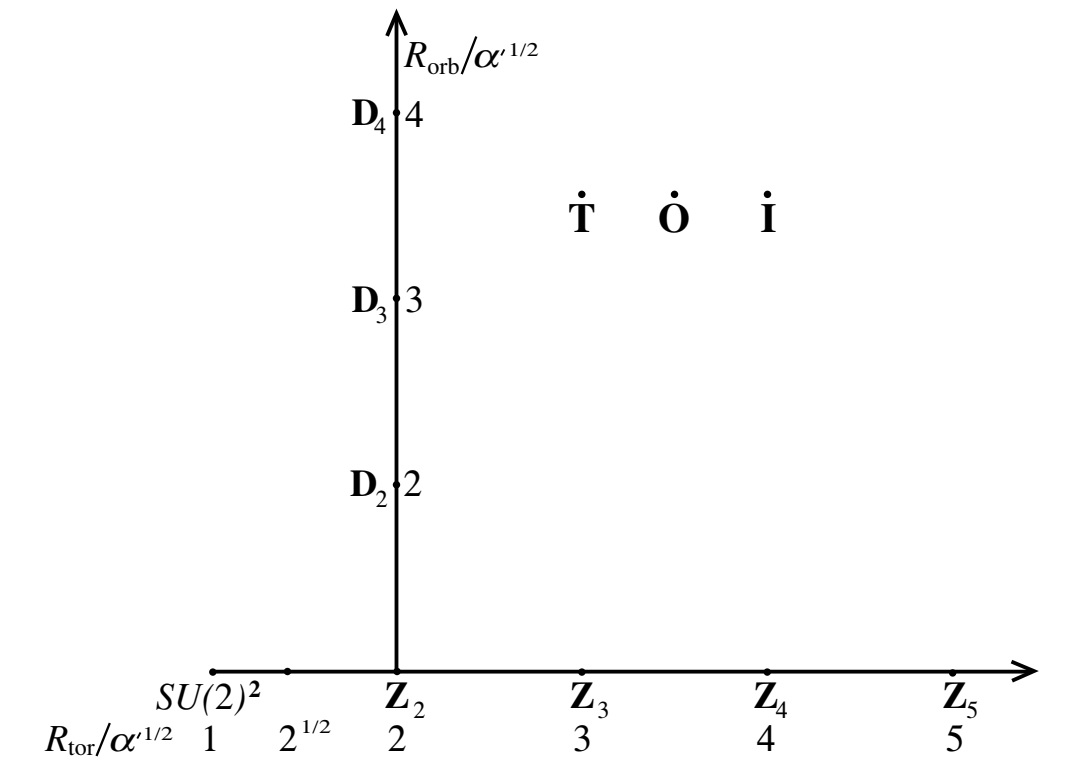
\includegraphics[width=0.8\textwidth]{figure/Fig8.2.jpg}
		\caption{Moduli space of $c=1$ CFT. The horizontal axis is the toroidal branch, while the vertical axis is the orbifold branch. The points marked in the figure are obtained by twisting with a discrete subgroup of the $SU(2)$ group, including three isolated points obtained from the tetrahedral group, the octahedral group, and the icosahedral group.
			Other special radii, such as the torus at $R=(2 \alpha^{\prime})^{1/2}$, will appear later.}\label{Fig8.2}
	\end{center}
\end{figure}

This equivalence holds only at these radii. For example, for a general $R$, toroidal theory only has $U(1) \times U(1)$ gauge symmetry, while the orbifold has no gauge symmetry. 
Therefore, the relationship between the two moduli spaces is as shown in Figure \ref{Fig8.2}. Moduli spaces with different branches meet at special points; in supersymmetric theories, this structure has very general and important features. 
Generally speaking, there will be different low-energy effective theories in each branch, manifested here as low-energy gauge symmetry. More light fields exist near special points. 
As we move away from special points along different branches, different subsets of them become massive.

The low-energy physics near the intersection of the toroidal and orbifold branches is very instructive. Describe it with the $S U(2)$ theory twisted by $r^{\prime}$ in \eqref{8.5.20}. 
The massless scalars remaining under this twisting are $j^{3} \tilde{\jmath}^{3}$ and $j^{i} \tilde{\jmath}^{j}$ for $i, j \in\{1,2\}$. 
Since they are untwisted, the potential is the same as before the twist, i.e., $\mathrm{det} M$. Scalar field $M_{i j}$ can still be diagonalized through $U(1) \times U(1)$ rotations, 
and the potential is flat only when one diagonal element is non-zero. 
However, the modulus $M_{33}$ cannot be rotated to $M_{11}$ or $M_{22}$ now, so these directions are physically different. 
Modulus $M_{33}$ preserves $U(1) \times U(1)$ and corresponds to movement along the toroidal branch. Modulus $M_{11}$ or $M_{22}$ breaks the gauge symmetry and corresponds to movement along the orbifold branch. 
Since this modulus is charged, its sign reversal is a gauge transformation, so physically different orbifolds end at the intersection of branches. We cannot transform two moduli simultaneously because their linear combination is not a flat direction. 
String theory on an orbifold is equivalent to string theory on a circle, which is quite remarkable. This shows that strings perceive spacetime geometry in a way that is not completely identical to ours.

Moving along the toroidal branch, there will be extra massless states at integer multiples of the $SU(2)$ radius $R=k \alpha^{\prime 1/2} $. 
These states have $(n, w)=(\pm 2 k, 0)$. 
We can think of these points as being obtained this way: under $T$-duality, $R=\alpha^{\prime 1/2} / k$, 
they are again obtained by twisting $S U(2) \times S U(2)$ theory using $\mathds{Z}_{k}$ symmetry:
\begin{equation}
	X^{25} \rightarrow X^{25}+\frac{2 \pi \alpha^{\prime 1/2}}{k} \:. \label{8.5.22}
\end{equation}
This multiplies $j^{1}+\mi j^{2}$ and $\tilde{\jmath}^{1}+\mi \tilde{\jmath}^{2}$ by $\exp (2 \pi \mi / k)$ , thus the surviving massless scalars are:
\begin{equation}
	j^{3} \tilde{\jmath}^{3}, \quad j^{1} \tilde{\jmath}^{1}+j^{2} \tilde{\jmath}^{2}, \quad 
	j^{1} \tilde{\jmath}^{2}-j^{2} \tilde{\jmath}^{1} \:. \label{8.5.23}
\end{equation}
The first of these changes the radius of the torus, thus it is always a flat direction. However, because the flatness condition \eqref{8.3.23} for the potential is not met in direction $M_{11}=M_{22}$ or $M_{12}=-M_{21}$, 
no other branches emerge from these points.

Offset \eqref{8.5.22} generates the $\mathds{Z}_{k}$ subgroup of $S U(2) \times S U(2) $. Let us examine twisting with other subgroups. 
Dihedral group $\mathbf{D}_{k}$ consists of offset \eqref{8.5.22} and reflection $X^{25} \rightarrow-X^{25}$, which gives the orbifold at radius $k \alpha^{\prime 1/2}$. 
The other three discrete subgroups are the tetrahedral group, octahedral group, and icosahedral group. They remove all moduli from the CFT, so twisting CFT is an isolated point, not a member of a continuous family. 
Unlike $\mathds{Z}_{k}$ and $\mathbf{D}_{k}$ twisting, which can be defined at all radii, these discrete subgroups containing $S U(2)$ elements exist only at discrete radii, 
thus the radius cannot vary after twisting. String theory with such a compactified space will only have one scalar—the dilaton. 

These are all known $c=1$ CFTs, and thus they give all known 25-dimensional bosonic string backgrounds.

\section{\texorpdfstring{Open Strings}{8.6 Open Strings}} \label{sec:8.6}

In toroidal compactification of open strings, there is a new feature: the possible existence of non-trivial Wilson lines, flat backgrounds for gauge fields. First study some $U(1)$ gauge theories with charged fields, examining constant backgrounds:
\begin{equation}
	A_{25}(x^{M})=-\frac{\theta}{2 \pi R}=-\mi \Lambda^{-1} \frac{\partial \Lambda}{\partial x^{25}}, \quad 
	\Lambda(x^{25})=\exp \biggl(-\frac{\mi \theta x^{25}}{2 \pi R}\biggr) \:, \label{8.6.1}
\end{equation}
where $\theta$ is a constant.
Locally, this is pure gauge, the field strength is zero, and field equations are trivial. However, gauge parameter $\Lambda$ does not satisfy spacetime periodicity, so the background has physical effects. 
The gauge invariant measuring this effect is the Wilson line:
\begin{equation}
	W_{q}=\exp \biggl(\mi q \oint \dif x^{25}\: A_{25}\biggr)=\exp (-\mi q \theta) \:. \label{8.6.2}
\end{equation}

First, consider a point particle with charge $q$; its gauge-fixed action is:
\begin{equation}
	S=\int \dif \tau \: \biggl(\frac{1}{2} \dot{X}^{M} \dot{X}_{M}+\frac{m^{2}}{2}-\mi q A_{M} \dot{X}^{M}\biggr) \:. \label{8.6.3}
\end{equation}
The gauge action is $-\mi q \int \dif x^{M}\, A_{M}$, so a path once around the compact dimension will pick out a phase equal to the Wilson line $W_{q} $. Canonical momentum is:
\begin{equation}
	p_{25}=-\frac{\partial L}{\partial v^{25}}=v^{25}-\frac{q \theta}{2 \pi R} \:, \label{8.6.4}
\end{equation}
where $v^{25}=\mi \dot{X}^{25}$ as in \eqref{8.4.6}.
The wave function must be periodic in the compact dimension, so $p_{25}=l/R$ for integer $l$, and:
\begin{equation}
	v_{25}=\frac{2 \pi l+q \theta}{2 \pi R} \:. \label{8.6.5}
\end{equation}
The Hamiltonian that annihilates physical states is:
\begin{equation}
	H=\frac{1}{2} (p_{\mu} p^{\mu}+v_{25}^{2}+m^{2}) \:, \label{8.6.6}
\end{equation}
since $v_{25}$ depends on $\theta$, $-p_{\mu} p^{\mu}$ is shifted. The same spectrum can be obtained in the field description. 
Note that $v_{25}$ is exactly the gauge-invariant momentum $-\mi \partial_{25}-q A_{25}$. 
We could also perform the gauge transformation $\Lambda^{-1}$ to set $A_{25}$ to zero; under this gauge, the charged field is no longer periodic, 
picking out the phase $\exp (\mi q \theta)$ under $x^{25} \rightarrow x^{25}+2 \pi R$. Physical quantities remain periodic.
The canonical momentum is now shifted, so we have:
\begin{equation}
	v_{25}=p_{25}=\frac{2 \pi l+q \theta}{2 \pi R}\:, \label{8.6.7}
\end{equation}
the same result is obtained for gauge-invariant momentum $v_{25}$ as before.

Now we return to strings and introduce $U(n)$ Chan-Paton factors. 
A general constant $A_{25}$ can be diagonalized by a gauge transformation:
\begin{equation}
	A_{25}=-\frac{1}{2 \pi R} \operatorname{diag}(\theta_{1}, \theta_{2}, \ldots, \theta_{n}) \:. \label{8.6.8}
\end{equation}
This gauge field lies in the diagonal group of $U(n)$, i.e., $U(1)^{n}$. 
The coupling of the gauge field with a general state's Chan-Paton factor is $[A_{M}, \lambda]$, 
so strings in the Chan-Paton state $|i j\rangle$ have charge $+1$ under $U(1)_{i}$, charge $-1$ under $U(1)_{j}$, and are neutral otherwise. Thus it has:
\begin{equation}
	v_{25}=\frac{2 \pi l-\theta_{j}+\theta_{i}}{2 \pi R} \:. \label{8.6.9}
\end{equation}
Then the open string spectrum is:
\begin{equation}
	m^{2}=\frac{(2 \pi l-\theta_{j}+\theta_{i})^{2}}{4 \pi^{2} R^{2}}+\frac{1}{\alpha^{\prime}}(N-1) \:. \label{8.6.10}
\end{equation}

Examine the gauge boson, which has $l=0$ and $N=1$, so:
\begin{equation}
	m^{2}=\frac{(\theta_{j}-\theta_{i})^{2}}{4 \pi^{2} R^{2}} \:. \label{8.6.11}
\end{equation}
In a general background, all $\theta$ are different, and only diagonal vectors with $i=j$ are massless. 
In this case, the unbroken gauge group is $U(1)^{n} $. 
If $r$ of the $\theta$ are equal, the corresponding vector $r \times r$ matrices are massless and carry $U(r)$ gauge symmetry. 
Assigning $n$ of the $\theta$ values to sets $r_{i}$, the gauge symmetry is:
\begin{equation}
	U(r_{1}) \times \ldots \times U(r_{s}), \quad \sum_{i=1}^{s} r_{i}=n \:. \label{8.6.12}
\end{equation}
As before, this has a low-energy interpretation. 
The gauge field $A_{25}$ is a 25-dimensional scalar in the adjoint representation of $U(n)$, and its vacuum expectation value breaks symmetry down to $U(r_{1}) \times \ldots \times U(r_{s})$.

Readers can fill in the details of the low-energy effective action. Note that if there are $k$ compact dimensions, the potential will contain:
\begin{equation}
	\operatorname{Tr}\Bigl([A_{m}, A_{n}]^{2}\Bigr) \:. \label{8.6.13}
\end{equation}
which comes from the field strength in the 26-dimensional Yang-Mills action. This forces gauge fields in different directions to commute in static solutions, allowing them to be simultaneously diagonalized. There are $kn$ moduli from gauge fields, and $k^{2}$ moduli from the metric and antisymmetric tensor.

\subsection*{$T$-duality}

Now examine the $R \rightarrow 0$ limit of the open string spectrum. If open string boundaries are Neumann boundaries, there is no quantum number analogous to $w$; they can always be untied from compact dimensions. 
So, as $R \rightarrow 0$, states with non-zero momentum acquire infinite mass, but there are no new continuous states. 
This is consistent with field theory behavior: corresponding states move in 25 spacetime dimensions.

We know that theories with open strings must have closed strings, which seems to cause a contradiction. It makes closed strings move in 26 spacetime dimensions while open strings move in 25 spacetime dimensions in the $R \rightarrow 0$ limit. 
From this it can be inferred that: the interior of an open string is identical to a closed string, composed of the same "matter", so it still vibrates in 26 dimensions. What distinguishes open strings is exactly their endpoints, 
so they must be restricted to a 25-dimensional hyperplane. 
Indeed, we can use new embedding coordinates to describe the $T$-duality theory:
\begin{equation}
	X^{\prime 25}(z, \bar{z})=X_{L}^{25}(z)-X_{R}^{25}(\bar{z}) \:. \label{8.6.14}
\end{equation}
Then:
\begin{equation}
	\partial_{n} X^{25}=-\mi \partial_{t} X^{\prime 25} \:, \label{8.6.15}
\end{equation}
where $n$ is the normal direction to the boundary, and $t$ is the tangent direction to the boundary. 
Neumann boundaries in the original coordinates become Dirichlet boundaries in the dual coordinates: the $X^{\prime 25}$ coordinate of each string endpoint is fixed. 

Let us first examine compactification without Wilson lines. Then all endpoints are constrained to the same hyperplane. To see this, integrate:
\begin{align}
	X^{\prime 25}(\pi)-X^{\prime 25}(0) &= \int_{0}^{\pi} \dif \sigma^{1}\: \partial_{1} X^{\prime 25}
	= -\mi \int_{0}^{\pi} \dif \sigma^{1}\: \partial_{2} X^{25} \nonumber \\
	&= -2 \pi \alpha^{\prime} v^{25}
	= -\frac{2 \pi \alpha^{\prime} l}{R}=-2 \pi l R^{\prime} \:. \label{8.6.16}
\end{align}
The total change of $X^{\prime 25}$ between two endpoints is an integer multiple of the dual dimension period $2 \pi R^{\prime}$, so the endpoints lie on the same hyperplane in the periodic $T$-dual space. 
For two different open strings, exchanging a graviton between them yields a connected worldsheet. We can apply the same argument as in \eqref{8.6.16} to this, so all string endpoints lie on the same hyperplane, 
as seen in Figure \ref{Fig8.3}. Endpoints move freely in the other 24 dimensions.

\begin{figure}[!htbp]
	\begin{center}
		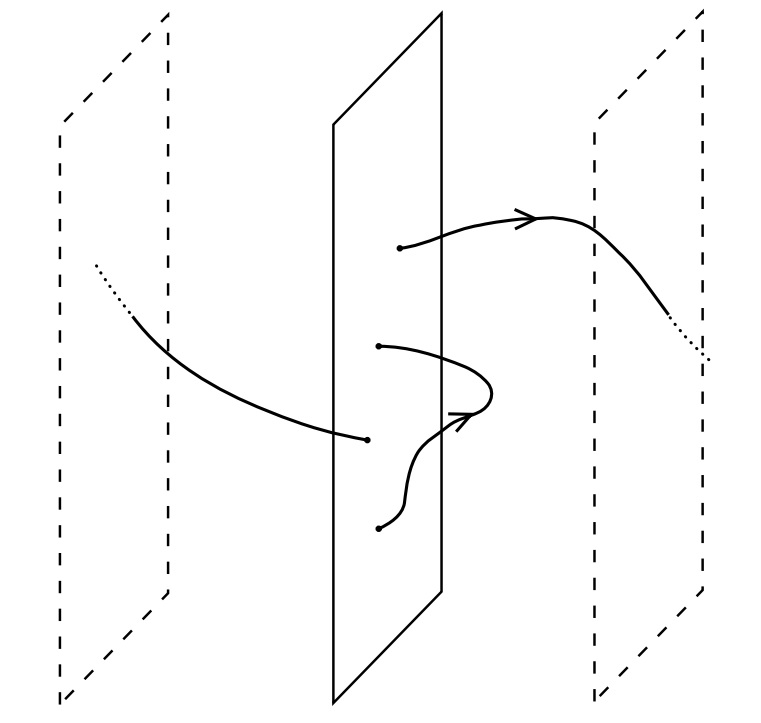
\includegraphics[width=0.7\textwidth]{figure/Fig8.3.jpg}
		\caption{Open strings with endpoints attached to a hyperplane. The planes marked with dashed lines are periodically equivalent planes. Two strings are shown in the figure, with winding numbers 1 and 0 respectively.}\label{Fig8.3}
	\end{center}
\end{figure}

Now let us look at the effect of Wilson lines. 
Due to the shift in $v_{25}$ in \eqref{8.6.9}, \eqref{8.6.16} is replaced by:
\begin{equation}
	\Delta X^{\prime 25}=X^{\prime 25}(\pi)-X^{\prime 25}(0)=-(2 \pi l-\theta_{j}+\theta_{i}) R^{\prime} \:. \label{8.6.17}
\end{equation}
In other words, discarding an extra normalization, endpoints on state $i$ are at:
\begin{equation}
	X^{\prime 25}=\theta_{i} R^{\prime}=-2 \pi \alpha^{\prime} A_{25, i i} \:. \label{8.6.18}
\end{equation}
Thus, there are generally $n$ different hyperplanes, as seen in Figure \ref{Fig8.4}.

\begin{figure}[!htbp]
	\begin{center}
		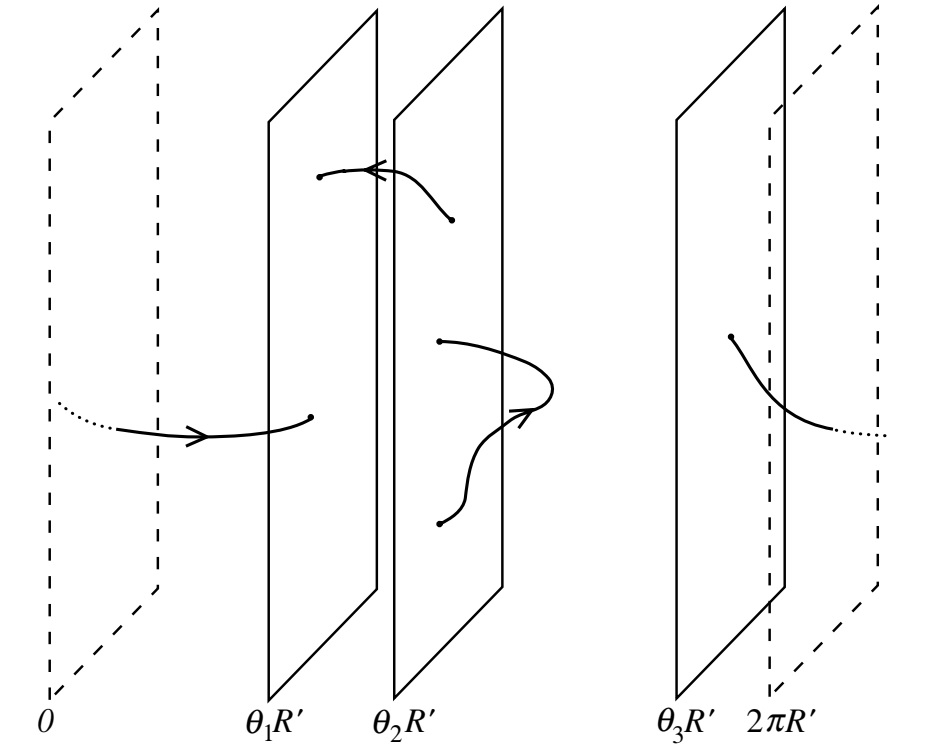
\includegraphics[width=0.8\textwidth]{figure/Fig8.4.jpg}
		\caption{$n=3$ hyperplanes at different positions, with different strings attached. Ignoring tachyons, the lightest strings with both ends on the same hyperplane are massless, while strings connecting two non-coincident hyperplanes are massive due to tension. When two hyperplanes coincide, the lightest strings connecting them become massless.}\label{Fig8.4}
	\end{center}
\end{figure}

Let us examine the mode expansion for the Chan-Paton state $|i j\rangle$, assuming it winds $l$ times around the compact dimension:
\begin{align}
	X^{\prime 25}(z, \bar{z}) &= \theta_{i} R^{\prime} - \frac{\mi R^{\prime}}{2 \pi}(2 \pi l-\theta_{j}+\theta_{i}) 
	\ln (z / \bar{z}) + \mi \biggl(\frac{\alpha^{\prime}}{2}\biggr)^{1/2} 
	\sum_{m=-\infty \atop m \neq 0}^{\infty} \frac{\alpha_{m}^{25}}{m}(z^{-m}-\bar{z}^{-m})  \nonumber \\
	&=\theta_{i} R^{\prime} + \frac{\sigma^{1}}{\pi} \Delta X^{\prime 25} - (2 \alpha^{\prime})^{1/2} 
	\sum_{m=-\infty \atop m \neq 0}^{\infty} \frac{\alpha_{m}^{25}}{m} \exp (-m \sigma^{2}) \sin m \sigma^{1} \:. \label{8.6.19}
\end{align}
The spectrum \eqref{8.6.10} becomes:
\begin{equation}
	m^{2}=\biggl(\frac{\Delta X^{\prime 25}}{2 \pi \alpha^{\prime}}\biggr)^{2}+\frac{1}{\alpha^{\prime}}(N-1) \:, \label{8.6.20}
\end{equation}
where $\Delta X^{\prime 25}$ is given by \eqref{8.6.17}. It is the shortest length of a string in a given sector.

Now examine how this picture generalizes if there are multiple compact dimensions. 
Let $X^{m}$ be periodic dimensions, where $p+1 \leq m \leq 25$. We write periodic dimensions in the form of dual coordinates. 
Neumann conditions on $X^{m}$ again become Dirichlet conditions on dual coordinates $X^{\prime m}$, so open string endpoints are restricted to $n$ parallel $(p+1)$-dimensional subspaces. 
For each subspace, Wilson lines in different directions become independent coordinates. 
Since translation invariance is broken by open string boundary conditions, the dual background is quite strange. This reflects the fact that: in the original open string theory, winding number is not conserved, and winding number $T$-duals to momentum. 
$T$-duality is just a different description of the same theory. Furthermore, when the compactification radius is very small, the $T$-duality picture should naturally be used.

\section{\texorpdfstring{D-branes}{8.7 D-branes}} \label{sec:8.7}
We now know that when an open string theory is compactified on a small torus, its physics can be described as compactification on a large torus, but with open string endpoints constrained to subspaces. In fact, these subspaces themselves are new dynamical objects. 
Consider the spectrum of massless open strings in a general configuration, where all $\theta_{i}$ are different, and for simplicity, only one coordinate is dualized. 
Ignoring tachyons, mass \eqref{8.6.20} is only zero when $N=1$ and $\Delta X^{\prime 25}=0 $. That is, both endpoints are on the same hyperplane and the winding number is zero. Thus we have massless states:
\begin{subequations} \label{8.7.1}
	\begin{align}
		&\alpha_{-1}^{\mu}|k; ii\rangle \:, \quad \mathscr{V} = \mi \partial_{t} X^{\mu}  \:, \label{8.7.1a} \\
		&\alpha_{-1}^{25} |k; ii\rangle \:, \quad \mathscr{V} = \mi \partial_{t} X^{25} = \partial_{n} X^{\prime 25} \:. \label{8.7.1b}
	\end{align}
\end{subequations}
They are obviously massless states in the original theory; $T$-duality just provides a different view of the same spectrum. For general Wilson lines, the only massless open string states will be $n$ massless $U(1)$ vectors. 
In \eqref{8.7.1}, we classified them according to whether they are tangent or normal to the hyperplane. 
The 25 states with tangential polarizations constitute a gauge field on the hyperplane, 
which has a simple and important interpretation in the $T$-duality theory: it is a set of coordinates for the shape of the hyperplane. This can be seen from the fact that a constant gauge field \eqref{8.6.18} corresponds to a uniform translation of the hyperplane. 
A background depending on $x^{\mu}$ can shift to a translation depending on $x^{\mu}$, a curved hyperplane, and the quantum of field $A_{ii}^{25}$ corresponds to a small oscillation of the hyperplane.

This is identical to phenomena occurring in spacetime. We start with strings in a flat background and discover that massless closed string states correspond to fluctuations in geometry. 
Here, we first discover hyperplanes, and then discover that specific open string states correspond to fluctuations of the hyperplanes. We should not be surprised that hyperplanes have dynamics. 
String theory includes gravity. Gravitational waves passing through a hyperplane will perturb spacetime itself, so it is difficult for hyperplanes to remain rigid. 
Thus, hyperplanes are indeed dynamical objects; these are D-branes. Performing duality on $25-p$ dimensions results in $p$-dimensional branes, called D$p$-branes. 
Using this terminology, the original $U(n)$ open string theory contains $n$ D25-branes. D25-branes fill the space, so there are no constraints on string endpoints: it just corresponds to general Chan-Paton factors. 
Since $T$-duality swaps Neumann and Dirichlet boundary conditions, $T$-duality in a direction tangent to a D$p$-brane reduces it to a D$(p{-}1)$-brane, 
while $T$-duality in a normal direction reduces it to a D$(p{+}1)$-brane. Non-trivial angle cases appear immediately. 

We could have started by studying Dirichlet boundaries themselves. Here the route we took was discovering them from $T$-duality, a method that better develops their properties. 
It can also be proven that through a continuous process, we can move from "ordinary" states to states containing D-branes. That is, taking the $R \rightarrow 0$ limit of the ordinary theory, which results in $n$ D-branes in non-compact space. 
In superstrings, we will use this to argue that D-branes are an important part of the non-perturbative definition of the theory. For bosonic strings, since there is no strong evidence that it has a non-perturbative definition, we do not discuss this. 
Bosonic string theory possibly exists only as a part of superstrings.

Let us look at $U(n)$ symmetry breaking in the $T$-duality picture. When no D-branes coincide, there are massless vectors only on each D-brane, yielding the gauge group $U(1)^{n}$. 
If $r$ D-branes coincide, there will be extra massless states, with the length of the strings connecting these branes being zero: when $n=0$, if both $i$ and $j$ are in set $r$, 
$\Delta X^{\prime 25}$ in mass formula \eqref{8.6.20} is zero. Thus, there are $r^{2}$ vectors, forming the adjoint representation of the $U(r)$ gauge group. 
This is the same as discovered in the dual Wilson line picture. However, surprisingly, there will be $r^{2}$ massless scalars in directions normal to the D-branes. We will discuss its meaning below.

\subsection*{D-brane Action}
On the worldvolume of a D$p$-brane, the massless fields are $U(1)$ vectors and $25{-}p$ worldvolume scalars describing fluctuations. The low-energy effective action for this system is always worth examining. 
We take the dual radius $R^{\prime}$ to be infinite and only consider a single D-brane in the corresponding 26-dimensional spacetime. Worldvolume fields interact with massless closed string fields, and its action was discussed in section \ref{sec:3.7}. 
Introduce coordinates $\xi^{a}$ on the brane, where $a=0, \ldots p$. Fields on the brane are the embedding $X^{\mu}(\xi)$ and the gauge field $A_{a}(\xi)$. 
We declare the action to be:
\begin{equation}
	\bm{S}_{p} = -T_{p} \int \dif^{p+1} \xi \: 
	\me^{-\Phi}[-\operatorname{det}(G_{ab} + B_{ab} + 2 \pi \alpha^{\prime} F_{a b})]^{1/2} \:, \label{8.7.2}
\end{equation}
\begin{tcolorbox}
	\begin{remark}
		We not know the full D-brane action in closed form. Above is low energy Effective Action.
	\end{remark}
\end{tcolorbox}
where $T_{p}$ is a constant to be determined. 
Here:
\begin{equation}
	G_{ab}(\xi) = \frac{\partial X^{\mu}}{\partial \xi^{a}} \frac{\partial X^{\nu}}{\partial \xi^{b}} G_{\mu \nu}(X(\xi)), \quad 
	B_{ab}(\xi) = \frac{\partial X^{\mu}}{\partial \xi^{a}} \frac{\partial X^{\nu}}{\partial \xi^{b}} B_{\mu \nu}(X(\xi)) \label{8.7.3}
\end{equation}
are the induced metric and induced antisymmetric tensor on the brane. 
All features of \eqref{8.7.2} can be understood based on general reasoning. First, considering only the spacetime metric and embedding, 
the simplest coordinate-independent action with fewest derivatives is the integral of $(-\operatorname{det} G_{a b})^{1/2}$, i.e., the worldvolume. 
Note that this term has an implicit relationship to $X^{\mu}(\xi)$ via the induced fields \eqref{8.7.3}. Expanding around a flat D-brane gives the action for fluctuations, 
just as the Nambu-Goto action describes string fluctuations.
\begin{tcolorbox}[breakable]
			A D$p$-brane is defined as a $p+1$ dimensional hyperplane in a $D$-dimensional spacetime to which open string endpoints are attached. These hyperplanes arise when Dirichlet boundary conditions are imposed in transverse directions, replacing the standard Neumann boundary conditions. 
			
				Dirichlet boundary conditions also arise through the T-duality of a compactified dimension with Neumann conditions. Specifically, the string satisfies Neumann boundary conditions in the directions along the hyperplane:
				\begin{equation}
					\frac{\partial X^\mu}{\partial \sigma} \Big|_{\sigma=0,\pi} = 0 \quad \text{for } \mu = 0, 1, \dots, p 
				\end{equation}
				and Dirichlet boundary conditions in the transverse directions:
				\begin{equation}
					X^\mu \Big|_{\sigma=0,\pi} = 0 \quad \text{for } \mu = p+1, \dots, D
				\end{equation}
				The endpoints of the open string in the original theory,
				\[
				X^\mu = X_L^\mu + X_R^\mu, \qquad \mu = 0, \ldots, D,
				\]
				are not fixed and satisfy Neumann boundary conditions. 
				However, the dual coordinates satisfy Dirichlet boundary conditions, and their endpoints are fixed on the D$p$-branes. The position of the D-brane is fixed by the dual coordinates $X'^{p+1}, \dots, X'^D$ defined in \eqref{8.6.18} such that:
				\begin{equation}
					X'^k = -2\pi \alpha' A_{k,ii} \quad \text{for } k = p+1, \dots, D
				\end{equation}
				where $i$ is the Chan-Paton index, linking the endpoints to a specific background $A_k$. For a single compactified dimension with $U(N)$ Chan-Paton factors, we consider an Abelian gauge background:
				\begin{equation}
					A_d = \frac{1}{2\pi R} \begin{pmatrix} \theta_1 & 0 & \dots & 0 \\ 0 & \theta_2 & \dots & 0 \\ \dots & \dots & \dots & \dots \\ 0 & 0 & \dots & \theta_N \end{pmatrix} 
				\end{equation}
				This field is pure gauge, $A_d = -i \Lambda^{-1} \partial_d \Lambda$, with:
				\begin{equation}
					\Lambda = \text{diag}(e^{i\theta_1 X^d / 2\pi R}, e^{i\theta_2 X^d / 2\pi R}, \dots, e^{i\theta_N X^d / 2\pi R}) 
				\end{equation}
				Although $A_d$ can be gauged away locally to zero via $\Omega(X) = \text{diag}(-\frac{\theta_1}{2\pi R}, \dots, -\frac{\theta_N}{2\pi R})$, it cannot be gauged away globally because $\Lambda(X)$ is not periodic:
				\begin{equation}
					\Lambda(X^d + 2\pi R) = \text{diag}(e^{i\theta_1}, \dots, e^{i\theta_N}) \Lambda(X^d) = W \cdot \Lambda(X^d) 
				\end{equation}
				The gauge invariant observable is the Wilson line $W = e^{i \oint dx^d A_d}$. Gauge invariant states pick up a phase after a periodic translation $X^d \to X^d + 2\pi R$, resulting in $U(N)$ symmetry breaking into $[U(1)]^N$. For a state $|k; ij\rangle$, endpoint $i$ picks up phase $e^{-i\theta_i / 2\pi R}$ and endpoint $j$ picks up $e^{-i\theta_j / 2\pi R}$, resulting in the wave function transformation:
				\begin{equation}
					|k; ij\rangle \to e^{i(\theta_j - \theta_i) / 2\pi R} |k; ij\rangle 
				\end{equation}
				This quantizes the momentum of that state as:
				\begin{equation}
					p_{(ij)}^D = \frac{n}{R} + \frac{\theta_j - \theta_i}{2\pi R} 
				\end{equation}
				The dual coordinates $X'^D$ then have endpoints fixed on hyperplanes at:
				\begin{equation}
					X'^D(\sigma=0; i) = 2\pi \alpha' A_{ii}^D \quad \text{and} \quad X'^D(\sigma=\pi; j) = 2\pi \alpha' A_{jj}^D 
				\end{equation}
				
				For multiple compactified dimensions, the mass spectrum generalizes to:
				\begin{equation}
					m^2 = \sum_{k=p+1}^D \left( \frac{\Delta X'^k}{2\pi \alpha'} \right)^2 + \frac{N - 1}{\alpha'} 
				\end{equation}
				Substituting the dual coordinates difference:
				\begin{equation}
					m^2 = \sum_{k=p+1}^D \left( \frac{2\pi l^k - \theta_i + \theta_j}{2\pi \alpha'} \right)^2 + \frac{N - 1}{\alpha'} 
				\end{equation}
				If $k$ endpoints have identical values ($\theta_1 = \dots = \theta_k = \theta$), massless states exist for $l^k = 0$ and $N=1$ even for strings stretched between different hyperplanes, as these hyperplanes are located at the same place. There are $k^2$ such massless states transforming under the adjoint representation of $U(k)$. This results in an unbroken $U(k)$ symmetry, providing a gauge theory on the D$p$-brane with scalar fields $\Phi_{ij}^m(\xi^a)$ describing D-brane dynamics.
			
			The derivation of the low-energy action starts with a free open string coupled to a constant background field strength $F_{\mu\nu} = \partial_\mu A_\nu - \partial_\nu A_\mu$. We have seen that we can also view this as a theory of open strings with end-points on a $D-$brane of dimension D, the entire	space-time. 
			
			Our goal is to work out a tree-level scattering amplitude using perturbation theory. We	are thus interested in a disc diagram with insertions at the boundary, or via a conformal	transformation a unit circle with four insertions on the boundary. We utilize the unit disc with polar coordinates $z = re^{i\theta}$ and the Green's function/kernel $f(z, z')$ with Neumann boundary conditions:
			\begin{equation}
				\partial \bar{\partial} f(z, z') = \delta(z - z') \quad \text{and} \quad \partial_r f(z, z') \big|_{r=1} = 0 
			\end{equation}
			The solution is:
			\begin{equation}
				f(z, z') = \frac{1}{2\pi} (\ln |z - z'| + \ln |z - \bar{z}'^{-1}|) 
			\end{equation}
			On the boundary ($r=1$), where $z' = \bar{z}'^{-1} = e^{i\theta}$ and $\bar{z}' = z'^{-1} = e^{-i\theta}$, this becomes:
			\begin{equation}
				f(\theta, \theta') = \frac{1}{2\pi} \ln (e^{i\theta} - e^{i\theta'})(e^{-i\theta} - e^{-i\theta'}) = \frac{1}{2\pi} \ln [2 - 2 \cos(\theta - \theta')] 
			\end{equation}
			Using the series expansion $\ln(1 + b^2 - 2b \cos x) = -2 \sum_{m=1}^\infty \frac{b^m}{m} \cos mx$ for $b=1$, we find:
			\begin{equation}
				f(\theta, \theta') = -\frac{1}{\pi} \sum_{n=1}^\infty \frac{1}{n} \cos n(\theta - \theta')\label{8.511} 
			\end{equation}
			We can alternatively prove this by expanding the logarithms:
			\begin{align}
				f(\theta, \theta') &= \frac{1}{2\pi} [ \ln e^{i\theta} + \ln(1 - e^{i\theta' - \theta}) + \ln e^{-i\theta} + \ln(1 - e^{-i\theta' - \theta}) ] \notag\\
				&= -\frac{1}{2\pi} \left[ \sum_{n=1}^\infty \frac{e^{in(\theta - \theta')}}{n} + \sum_{n=1}^\infty \frac{e^{-in(\theta - \theta')}}{n} \right] = -\frac{1}{\pi} \sum_{n=1}^\infty \frac{\cos [n(\theta - \theta')]}{n} 
			\end{align}
			The inverse Green's function $f^{-1}(\theta, \theta')$ must satisfy $\int d\theta' f(\theta, \theta') f^{-1}(\theta', \theta'') = \delta(\theta - \theta'') - \frac{1}{2\pi}$. It is given by:
			\begin{equation}
				f^{-1}(\theta, \theta') = -\frac{1}{\pi} \sum_{n=1}^\infty n \cos n(\theta - \theta') \label{8.513}
			\end{equation}
			To check this, evaluate the integral:
			\begin{equation}
				\int_0^{2\pi} d\theta' f(\theta, \theta') f^{-1}(\theta', \theta'') = \frac{1}{\pi^2} \int_0^{2\pi} d\theta' \sum_{m,n=1}^\infty \frac{m}{n} \cos [n(\theta - \theta')] \cos [m(\theta' - \theta'')] 
			\end{equation}
			Using $\cos n(\theta - \theta') = \cos n\theta \cos n\theta' + \sin n\theta \sin n\theta'$ and the orthogonality relations $\int_0^{2\pi} d\theta' \cos m\theta' \cos n\theta' = \int_0^{2\pi} d\theta' \sin m\theta' \sin n\theta' = \pi \delta_{m,n}$:
			\begin{equation}
				= \frac{1}{\pi} \sum_{m=1}^\infty ( \cos m\theta \cos m\theta'' + \sin m\theta \sin m\theta'' ) = \frac{1}{\pi} \sum_{m=1}^\infty \cos m(\theta - \theta'') 
			\end{equation}
			With the Fourier decomposition $\frac{1}{\pi} \sum_{m=1}^\infty \cos m(\theta - \theta'') = \delta(\theta - \theta'') - \frac{1}{2\pi}$, the following is satisfied:
			\begin{equation}
				\int_0^{2\pi} d\theta' f(\theta, \theta') f^{-1}(\theta', \theta'')=\delta(\theta-\theta')-\frac{1}{2\pi}\label{8.519}
			\end{equation}
			
			\begin{proof}	
			The bosonic string coupled to a photon field in the conformal gauge has action:
			\begin{equation}
				S[X, A] = \frac{1}{4\pi\alpha'} \int d^2z \partial X^\mu \bar{\partial} X_\mu - i \oint d\theta \partial_\theta A_\mu \big|_{r=1} 
			\end{equation}
			Note that the contribution of the minimally coupled photon field can be seen to correspond
			to the insertion of an open string vertex operator. As we integrate out the spacetime fields
			$X^{\mu}$ the resulting partition function is a functional of the gauge field only, and because of gauge invariance of the Wilson loop it must be a functional of the field strength $F_{\mu\nu}$. We evaluate the Euclidean path integral $Z[F] = \frac{1}{g_s} \int \mathcal{D}X^\mu e^{-S}$ using the background method $X^\mu = X_0^\mu + \xi^\mu$. In the radial gauge $\xi^\mu A_\mu(X_0 + \xi) = 0$ and assuming constant $F_{\mu\nu}$, the path integral measure $\mathcal{D}X^\mu$ is split between the interior and the boundary:
			\begin{equation}
				\mathcal{D}X^\mu = \prod_{|z|<1} \mathcal{D}X^\mu(z, \bar{z}) \prod_{boundary} \mathcal{D}\xi^\mu(\theta) 
			\end{equation}
			Reducing the interior integration to a boundary integral by introducing field $\eta(\theta)$ and representing the delta function $\delta^{(D)}(\xi^\mu - \eta^\mu)$ as a Gaussian over auxiliary fields $\nu^\mu$:
			\begin{align*}
				Z[F] &= \int \mathcal{D}\xi^\mu e^{-\frac{1}{4\pi\alpha'} \int d\theta \partial \xi^\mu \bar{\partial} \xi_\mu} \int \mathcal{D}\eta^\mu \delta^{(D)}(\xi^\mu - \eta^\mu) \times \text{o.c.} \\
				&= \int \mathcal{D}\xi^\mu \mathcal{D}\eta^\mu e^{-\frac{1}{4\pi\alpha'} \int d\theta \partial \xi^\mu \bar{\partial} \xi_\mu} \frac{1}{(2\pi)^D} \int \mathcal{D}\nu^\mu e^{i \int d\theta \nu^\mu (\xi_\mu - \eta_\mu)} \times \text{o.c.} \\
				&= \frac{1}{(2\pi)^D} \int \mathcal{D}\eta^\mu \mathcal{D}\nu^\mu \int \mathcal{D}\xi^\mu e^{\int d\theta \left[ -\frac{1}{4\pi\alpha'} \partial \xi^\mu \bar{\partial} \xi_\mu + i \nu^\mu (\xi_\mu - \eta_\mu) \right]} \times \text{o.c.}
			\end{align*}
			where o.c. stands for other contributions. Rescaling $\xi$ and $\eta$ by $\sqrt{2\pi \alpha'}$ and performing Gaussian integrations:
			\begin{align*}
				Z[F] &\propto \int \mathcal{D}\eta^\mu \mathcal{D}\nu^\mu \int \mathcal{D}\xi^\mu e^{-\xi^\mu \left( -\frac{\partial\bar{\partial}}{2} \right) \xi_\mu + i \sqrt{2\pi\alpha'} \nu^\mu (\xi_\mu - \eta_\mu)} \times \text{o.c.} \\
				&\propto \int \mathcal{D}\eta^\mu \mathcal{D}\nu^\mu \left( \frac{\pi}{\text{det}(-\partial\bar{\partial}/2)} \right)^{\frac{D}{2}} e^{-\nu^\mu \frac{4\pi\alpha'}{\partial\bar{\partial}} \nu_\mu - i \sqrt{2\pi\alpha'} \nu^\mu \eta_\mu} \times \text{o.c.} \\
				&\propto \int \mathcal{D}\eta^\mu \left( \frac{\pi}{\text{det}(-\partial\bar{\partial}/2)} \right)^{\frac{D}{2}} \left( \frac{\pi}{\text{det}(4\pi\alpha'/\partial\bar{\partial})} \right)^{\frac{D}{2}} e^{-\frac{2\pi\alpha'\eta^\mu\eta_\mu}{4\pi\alpha'/\partial\bar{\partial}}} \times \text{o.c.} \\
				&\propto \int \mathcal{D}\eta^\mu e^{-\eta^\mu \frac{\partial\bar{\partial}}{2} \eta_\mu} \times \text{o.c.}
			\end{align*}
			Renaming $\eta$ to $\xi$, the kinetic term contribution is $\int \mathcal{D}\xi^\mu e^{-\frac{1}{2} \xi^\mu f^{-1} \xi_\mu}$. The gauge field term rescales by $2\pi\alpha'$, becoming:
			\begin{equation}
				i \int_0^{2\pi} d\theta F_{\mu\nu} \xi^\mu \dot{\xi}^\nu = \frac{i}{2} \int_0^{2\pi} d\theta ( \partial_\mu A_\nu \xi^\mu \dot{\xi}^\nu - \partial_\mu A_\nu \xi^\nu \dot{\xi}^\mu ) = i \int_0^{2\pi} d\theta \partial_\mu A_\nu \xi^\mu \dot{\xi}^\nu + o(\partial F) 
			\end{equation}
			Combining these gives the boundary path integral:
			\begin{equation}
				Z[F] \propto \int \mathcal{D}\xi^\mu \exp \left( -\frac{1}{2} \xi^\mu f^{-1} \xi_\mu + \frac{i}{2} F_{\mu\nu} \int_0^{2\pi} d\theta \xi^\mu \dot{\xi}^\nu \right) 
			\end{equation}
			Using Lorentz invariance, we bring the antisymmetric matrix $F_{\mu\nu}$ into its Jordan normal form, consisting of $D/2$ antisymmetric $2 \times 2$ blocks:
			\begin{equation}
				F_{\mu\nu} = \begin{pmatrix} 
					0 & -f_1 & & 0 & 0 \\
					f_1 & 0 & & 0 & 0 \\
					& & \ddots & & \\
					0 & 0 & & 0 & -f_{D/2} \\
					0 & 0 & & f_{D/2} & 0 
				\end{pmatrix}
			\end{equation}
			
			Substituting this into the interaction term, we expand the product $\xi^\mu F_{\mu\nu} \dot{\xi}^\nu$:
			\begin{align}
				\xi^\mu F_{\mu\nu} \dot{\xi}^\nu &= (\xi^1 \ \dots \ \xi^D) \begin{pmatrix} 
					0 & -f_1 & & 0 & 0 \\
					f_1 & 0 & & 0 & 0 \\
					& & \ddots & & \\
					0 & 0 & & 0 & -f_{D/2} \\
					0 & 0 & & f_{D/2} & 0 
				\end{pmatrix} \begin{pmatrix} \dot{\xi}^1 \\ \vdots \\ \dot{\xi}^D \end{pmatrix} \\
				&= -\xi^1 \dot{\xi}^2 f_1 + \xi^2 \dot{\xi}^1 f_1 - \xi^3 \dot{\xi}^4 f_2 + \xi^4 \dot{\xi}^3 f_2 + \dots - \xi^{D-1} \dot{\xi}^D f_{D/2} + \xi^D \dot{\xi}^{D-1} f_{D/2} \\
				&= \sum_{k=1}^{D/2} \left( -\xi^{2k-1} \dot{\xi}^{2k} + \xi^{2k} \dot{\xi}^{2k-1} \right) f_k 
			\end{align}
			
			The path integral factorizes into $D/2$ independent $2 \times 2$ blocks. Applying partial integration to the second term in the sum for each block:
			\begin{equation}
				Z[F] \propto \prod_{k=1}^{D/2} \int \mathcal{D}\xi^{2k-1} \mathcal{D}\xi^{2k} \exp \left[ -\left( \frac{1}{2} \xi^{2k-1} f^{-1} \xi^{2k-1} + \frac{1}{2} \xi^{2k} f^{-1} \xi^{2k} + i f_k \xi^{2k-1} \dot{\xi}^{2k} \right) \right]
			\end{equation}
			
			We integrate over $\xi^{2k}$ using the Gaussian functional identity $\int \mathcal{D}x e^{-\frac{1}{2} x A x + Jx} \propto (\det A)^{-1/2} e^{\frac{1}{2} J A^{-1} J}$. Renaming $\xi^{2k-1}$ as $\xi$:
			\begin{align}
				Z[F] &\propto \prod_{k=1}^{D/2} \int \mathcal{D}\xi \sqrt{\frac{2\pi}{\det(f^{-1})}} \exp \left( -\frac{1}{2} \xi f^{-1} \xi - \frac{f_k^2 \dot{\xi} \dot{\xi}}{4 f^{-1}/2} \right) \\
				&\propto \prod_{k=1}^{D/2} \int \mathcal{D}\xi \sqrt{2\pi \det(f)} \exp \left( -\frac{1}{2} \xi f^{-1} \xi - \frac{1}{2} f_k^2 \dot{\xi} f \dot{\xi} \right) \\
				&\propto \prod_{k=1}^{D/2} \int \mathcal{D}\xi \sqrt{2\pi \det(f)} \exp \left[ -\frac{1}{2} \xi \left( f^{-1} + f_k^2 \ddot{f} \right) \xi \right]
			\end{align}
			where we have defined $\ddot{f}(\theta, \theta') = \partial_\theta \partial_{\theta'} f(\theta, \theta')$ through partial integration. The final integration over the remaining coordinates $\xi$ yields:
			\begin{equation}
				Z[F] \propto \prod_{k=1}^{D/2} \sqrt{2\pi \det(f)} \sqrt{\frac{2\pi}{\det(f^{-1} + f_k^2 \ddot{f})}} \propto \prod_{k=1}^{D/2} \left[ \det(f^{-1}f + f_k^2 \ddot{f} f) \right]^{-1/2}
			\end{equation}
			Rescaling the tensor $F_{\mu\nu} \to 2\pi\alpha' F_{\mu\nu}$, we have
			\begin{equation}
				Z[F] = Z[0] \prod_{k=1}^{D/2} (\det \Delta_k)^{-1/2} \quad \text{with} \quad \Delta_k = f^{-1}f + (2\pi\alpha' f_k)^2 \ddot{f} f\label{8.538}
			\end{equation}
			To proceed we need to compute $f \ddot{f}$, which can be done by using the integral kernels \eqref{8.511} and $\ddot{f} = \partial_\theta \partial_{\theta'} f(\theta, \theta')$,
			\begin{equation}
				\dot{f} = \frac{1}{\pi} \sum_{n=1}^{\infty} \sin n(\theta - \theta') \quad \text{and} \quad \ddot{f} = -\frac{1}{\pi} \sum_{n=1}^{\infty} n \cos n(\theta - \theta')
			\end{equation}
			
			From \eqref{8.513} we see that $\ddot{f} = f^{-1}$ and therefore $\ddot{f} f = f^{-1} f = \delta(\theta - \theta') - \frac{1}{2\pi} = \bar{\delta}(\theta - \theta')$, where we have used \eqref{8.519}. We therefore get the following kernel form of the $\Delta_k$ operator:
			\begin{equation}
				\Delta_k(\theta, \theta') = [1+ (2\pi\alpha' f_k)^2] \bar{\delta}(\theta - \theta')
			\end{equation}
			To evaluate the determinant of this operator, we expand any field in the orthonormal basis on the boundary of the disk. The basis elements are $E_m = \pi^{-1/2} \cos m\theta$ and $F_m = \pi^{-1/2} \sin m\theta$ for $m \ge 1$. For any basis element $E_n$, the action of the $\bar{\delta}(\theta - \theta')$ operator is:
			\begin{align}
				\int_0^{2\pi} d\theta' \bar{\delta}(\theta - \theta') E_n(\theta') &= \int_0^{2\pi} d\theta' \delta(\theta - \theta') E_n(\theta') -\underbrace{ \frac{1}{2\pi} \int_0^{2\pi} E_n(\theta') d\theta'}_{=0 \text{ for $n\ge1$}}\notag\\
				&=E_n(\theta)
			\end{align}
			As a result, the basis elements $E_n$ and $F_n$ are thus eigenfunctions of $\Delta_k$ with eigenvalues:
			\begin{equation}
			\int_0^{2\pi} \Delta_k(\theta, \theta') E_m(\theta') d\theta' = E_m(\theta) + (2\pi\alpha' f_k)^2 E_m(\theta) = [1 + (2\pi\alpha' f_k)^2] E_m(\theta)
			\end{equation}
			Because each $n$ corresponds to two degenerate eigenfunctions ($E_n$ and $F_n$), the determinant over the fluctuation space is the infinite product:
			\begin{equation}
				\det \Delta_k = \prod_{n=1}^{\infty} [1 + (2\pi\alpha' f_k)^2]^2
			\end{equation}
			Plugging this in \eqref{8.538} we find that
			\begin{equation}
				Z[F] = Z[0] \prod_{k=1}^{D/2} (\det \Delta_k)^{-1/2} = Z[0] \prod_{k=1}^{D/2} \prod_{m=1}^{\infty} [1 + (2\pi\alpha' f_k)^2]^{-1}
			\end{equation}
			Regularizing via the Riemann zeta function $\zeta(s) = \sum n^{-s}$ where $\zeta(0) = -1/2$:
			\begin{equation}
				\prod_{m=1}^\infty c^{-1} = e^{ - \zeta(0) \ln c } = c^{1/2} 
			\end{equation}
			Which results in
			\begin{equation}
				Z[F]= Z[0] \prod_{k=1}^{D/2} \prod_{m=1}^{\infty} [1 + (2\pi\alpha' f_k)^2]^{-1} = Z[0] \prod_{k=1}^{D/2} [ 1 + (2\pi \alpha' f_k)^2 ]^{1/2}
			\end{equation}
			The RHS involves an infinite product of Eigenvalues and originates from the determinant of the following operator:
			\begin{align*}
				\det (\delta_{\mu\nu} + 2\pi\alpha' F_{\mu\nu}) &= \begin{pmatrix} 
					1 & -2\pi\alpha' f_1 & & 0 & 0 \\
					2\pi\alpha' f_1 & 1 & & 0 & 0 \\
					& & \ddots & & \\
					0 & 0 & & 1 & -2\pi\alpha' f_{D/2} \\
					0 & 0 & & 2\pi\alpha' f_{D/2} & 1 
				\end{pmatrix} \\
				&= \prod_{k=1}^{D/2} [1 + (2\pi\alpha' f_k)^2]
			\end{align*}
			Applying this to the partition function leads to:
			\begin{equation}
				Z[F] = \frac{1}{(4\pi^2\alpha')^{D/2} g_s} \int \mathcal{D}X_0^\mu [ \det(\delta_{\mu\nu} + 2\pi\alpha' F_{\mu\nu}) ]^{1/2}
			\end{equation}
			
			For the compactified string, we apply T-duality. Splitting the matrix $\delta_{\mu\nu} + 2\pi\alpha' F_{\mu\nu}$ into parallel ($a, b$) and transverse ($m, n$) components:
			$$\begin{aligned}
				\delta_{\mu\nu} + 2\pi\alpha' F_{\mu\nu} &= \left( \begin{array}{c|c} 
					\delta_{ab} + 2\pi\alpha' F_{ab} & 2\pi\alpha' F_{ma} \\ \hline 
					2\pi\alpha' F_{am} & \delta_{mn} + 2\pi\alpha' F_{mn} 
				\end{array} \right) \\
				&= \left( \begin{array}{c|c} 
					\delta_{ab} + 2\pi\alpha' F_{ab} & -2\pi\alpha' \partial_a A_m \\ \hline 
					2\pi\alpha' \partial_a A_m & \delta_{mn} 
				\end{array} \right)
			\end{aligned}$$
			
			where we have used the fact that $\partial_m X = 0$ for $m = p+1, \dots, D$. We now introduce a $(p+1) \times (p+1)$ matrix $N$ and a $(p+1) \times (D-p)$ matrix $A$ with elements
			\begin{equation*}
				N_{ab} = \eta_{ab} + 2\pi\alpha' F_{ab}, \quad A_{ma} = 2\pi\alpha' \partial_a A_m
			\end{equation*}  
			
			We can thus write
			\begin{equation*}
				\delta_{\mu\nu} + 2\pi\alpha' F_{\mu\nu} = \left( \begin{array}{c|c}
					N & -A^T \\ \hline
					A & \mathbf{1}
				\end{array} \right)
			\end{equation*}  
			with $\mathbf{1}$ being the $(D-p) \times (D-p)$ unit matrix. We now use the matrix identity
			\begin{equation*}
				\det \begin{pmatrix} N & B \\ C & D \end{pmatrix} = \det(D) \det(N - B D^{-1} C)
			\end{equation*}  
			
			Therefore, applying this to our specific block matrix:
			\begin{align}
					\det(\delta_{\mu\nu} + 2\pi\alpha' F_{\mu\nu}) &= \det(N + A^T \mathbf{1}^{-1} A) = \det(\eta_{ab} + 2\pi\alpha' F_{ab} + (2\pi\alpha')^2 \partial_a A_m \partial_b A^m)\notag\\
				 &= \det(\eta_{ab} + 2\pi\alpha' F_{ab} + (2\pi\alpha')^2 \partial_a A^m \partial_b A_m) 
			\end{align}
			Substituting the T-dual coordinate $X'^m = -2\pi \alpha' A_m$, we find:
			\begin{equation}
				\det(\delta_{\mu\nu} + 2\pi\alpha' F_{\mu\nu}) = \det(\eta_{ab} + 2\pi\alpha' F_{ab} + \partial_a X'^m \partial_b X'^m) 
			\end{equation}
			Including the brane tension $T_p = \frac{1}{\sqrt{\alpha'}} \frac{1}{(2\pi\sqrt{\alpha'})^p}$, we can write the action as:
			\begin{equation}
				S = -\frac{T_p}{g_s} \int d^{p+1}\xi \sqrt{-\det(\eta_{ab} + \partial_a X'^m \partial_b X'^m + 2\pi \alpha' F_{ab})} 
			\end{equation}
			In curved spacetimes with fields $G_{\mu\nu}, B_{\mu\nu}$, and dilaton $\Phi$, the result generalizes to the effective action:
			\begin{equation}
				S = -T_p \int d^{p+1}\xi e^{-\Phi} \sqrt{-\det(G_{ab} + B_{ab} + 2\pi \alpha' F_{ab})} 
			\end{equation}
			where $G_{ab}$ and $B_{ab}$ are the pull-backs to the worldvolume:
			\begin{equation}
				G_{ab}(\xi) = G_{\mu\nu}(X(\xi)) \frac{\partial X^\mu}{\partial \xi^a} \frac{\partial X^\nu}{\partial \xi^b}, \quad B_{ab}(\xi) = B_{\mu\nu}(X(\xi)) \frac{\partial X^\mu}{\partial \xi^a} \frac{\partial X^\nu}{\partial \xi^b} 
			\end{equation}
	\end{proof}
\end{tcolorbox}
The dependence on the dilaton $\me^{-\Phi} \propto g_{\mathrm{c}}^{-1}$ appears because this is an open string tree action. 
Self-interactions of open string fields, and their coupling with closed string fields, originally come from the disk.

The dependence on $F_{ab}$ can be understood through $T$-duality. Consider a D-brane spread along $X^{1}$ and $X^{2}$ directions, with other directions unspecified, and let there be a constant gauge field $F_{12}$ on it. 
Go to the gauge $A_{2}=X^{1} F_{12}$. Now take $T$-duality along the $X^{2}$ direction. 
The Neumann condition in this direction becomes a Dirichlet condition, so the D-brane loses one dimension. 
However, the relationship between the potential and coordinates \eqref{8.6.18} implies that the D-brane is tilted in the (1-2)-plane:
\begin{equation}
	X^{\prime 2}=-2 \pi \alpha^{\prime} X^{1} F_{12} \:. \label{8.7.4}
\end{equation}
This tilt gives the action a geometric factor:
\begin{equation}
	\int \dif X^{1}\: \Bigl[1 + (\partial_{1} X^{\prime 2})^{2}\Bigr]^{1/2} 
	=\int \dif X^{1}\: \Bigl[1 + (2 \pi \alpha^{\prime} F_{12})^{2}\Bigr]^{1/2} \:. \label{8.7.5}
\end{equation}
For any D-brane, the action can be reduced to the product of factors \eqref{8.7.5} in each plane by pushing it to align with the coordinate axes and rotating, 
equivalent to the $F_{ab}$ term in the determinant. The determinant composed of gauge fields is called the Born-Infeld action, which was originally intended to solve the short-range divergence problem of quantum electrodynamics.

Finally, the dependence on $B_{ab}$ is given by the following discussion. 
In the worldsheet action of strings, closed string field $B_{\mu \nu}$ and open string field $A^{\mu}$ appear in the following form:
\footnote{For readers familiar with differential forms, this is:
	\[ \frac{\mi}{2 \pi \alpha^{\prime}} \int_{M} B + \mi \int_{\partial M} A \:. \]
	The subsequent equation can be translated in a similar way.}
\begin{equation}
	\frac{\mi}{4 \pi \alpha^{\prime}} \int_{M} \dif^{2} \sigma \: g^{1/2} \epsilon^{ab} \partial_{a} X^{\mu} \partial_{b} X^{\nu} 
	B_{\mu\nu} + \mi \int_{\partial M} \dif X^{\mu} \:A_{\mu} \:. \label{8.7.6}
\end{equation}
Each of these fields is accompanied by a spacetime gauge invariance, which must be preserved to be consistent with spacetime theory. The usual gauge transformation:
\begin{equation}
	\delta A_{\mu}=\partial_{\mu} \lambda \label{8.7.7}
\end{equation}
is an invariance of action \eqref{8.7.6}, where the boundary term differs by the integral of a total derivative. The antisymmetric tensor variation:
\begin{equation}
	\delta B_{\mu \nu} = \partial_{\mu} \zeta_{\nu} - \partial_{\nu} \zeta_{\mu} \label{8.7.8}
\end{equation}
makes the "bulk" action differ by a total derivative, but on a worldsheet with boundaries, this yields a surface term. 
To make it cancel, under tensor gauge symmetry, the open string field $A_{\mu}$ must transform as:
\begin{equation}
	\delta A_{\mu}=-\zeta_{\mu} / 2 \pi \alpha^{\prime} \:. \label{8.7.9}
\end{equation}
Now, only the combination:
\begin{equation}
	B_{\mu \nu}+2 \pi \alpha^{\prime} F_{\mu \nu} \equiv 2 \pi \alpha^{\prime} \mathscr{F}_{\mu \nu}  \label{8.7.10}
\end{equation}
is invariant under both symmetries, so it must be this combination that appears in the action. Thus, the form of the action \eqref{8.7.2} is completely determined. 
As a check, since the same combination appears in the worldsheet action under conformal gauge, it is natural that the combination $G_{\mu \nu}+B_{\mu \nu}$ should appear. 
The action \eqref{8.7.2} could also be determined by taking low-energy limits of various open string and open-closed string amplitudes, but this would be much more laborious.

For $n$ discrete D-branes, the action is $n$ copies of a single D-brane action. 
However, we have seen that when D-branes coincide, there will be $n^{2}$ massless vectors and scalars on the brane instead of $n$, 
and we will write the effective action for this case. Fields $X^{\mu}(\xi)$ and $A_{a}(\xi)$ will now be $n \times n$ matrices. 
For gauge fields, the meaning is obvious—it becomes a non-Abelian $U(n)$ gauge field. However, for coordinates $X^{\mu}$, the meaning is unclear: the embedding coordinate set for $n$ D-branes into spacetime extends into $n \times n$ matrices. 
Non-commutative geometry has been proven to play an important role in the dynamics of D-branes, and here is a conjecture: it is an important clue to the characteristics of spacetime.

We can obtain more enlightenment by examining the effective action. 
There are now non-derivative terms in the action, which is the potential for the coordinates, and this can be inferred from $T$-duality for constant $A_{m}$ fields. 
For such vector potentials, the field strength is $[A_{m}, A_{n}]$, which becomes $(2 \pi \alpha^{\prime})^{-2}[X_{m}, X_{n}]$ in the $T$-duality picture. 
Expanding in the field strength, the leading order of the action is approximately:
\begin{equation}
	V \propto \operatorname{Tr}([X_{m}, X_{n}][X^{m}, X^{n}]) \:. \label{8.7.11}
\end{equation}
The second derivative of this potential at $X^{m}=0$ is zero, making all $k n^{2}$ scalars massless; as before $k=25{-}p$ is the dual dimension. 
However, the space of flat dimensions is smaller. The potential is a sum of squares, so it is zero only when all $[X^{m}, X^{n}]$ are zero. We can go to the gauge where $X^{m}$ are all diagonal using $U(n)$ symmetry. 
Thus there will be $kn$ flat directions, exactly the number of diagonal elements. 
In this way, the $kn$ diagonal elements can be interpreted as the coordinates for $n$ D$p$-branes. 
Thus \eqref{8.7.11} correctly intervenes in the physics of separating D-branes and coinciding D-branes.

When $X^{m}$ commute, the action should reduce to $n$ separate D-branes, thus:
\begin{align}
	\bm{S}_{p} &= -T_{p} \int \dif^{p+1} \xi \: \operatorname{Tr} \Bigl\{ \me^{-\Phi}
	[-\operatorname{det}(G_{ab} + B_{ab} + 2 \pi \alpha^{\prime} F_{ab})]^{1/2} \nonumber \\
	&\qquad \qquad \qquad \quad + O([X^{m}, X^{n}]^{2})\Bigr\} \:. \label{8.7.12}
\end{align}
The determinant is taken over worldvolume indices $ab$, and the trace is taken over $n$ Chan-Paton indices. The trace is a suitable $U(n)$ invariant, which for diagonal matrices reduces to the sum over separate D-branes. 
The complete dependence on the commutator is much more complex than the simple potential \eqref{8.7.11}, involving couplings with other fields and higher-order corrections to the commutator. 
However, the key property, the form of the flat directions, is unaffected. 
By starting from the Born-Infeld action in the complete Neumann case and performing $T$-duality, we can obtain the full dependence. 
Incidentally, higher-order derivative terms containing field strength commutators cannot be determined just by $T$-duality.

\subsection*{D-brane Tension}
Calculating the constant $T_{p}$ is very meaningful, and for superstrings, its exact value is very important. Before performing explicit calculation, note that the recurrence relation for $T_{p}$ can be obtained from $T$-duality. 
Note that in a constant dilaton background, the tension of a D$p$-brane is $T_{p} \me^{-\Phi}$: this is the negative of the action per unit volume for a static D$p$-brane. 
Now examine such a D$p$-brane where $p$ directions tangent to the D$p$-brane are periodically equivalent. That is, the D$p$-brane is wrapped on a $p$-torus in spacetime. Its mass is its tension multiplied by the area of its torus:
\begin{equation}
	T_{p} \me^{-\Phi} \prod_{i=1}^{p}(2 \pi R_{i}) \:. \label{8.7.13}
\end{equation}
Now, take $T$-duality along one of the periodic directions $X^{p}$. 
This does not change the mass, just a new description of the same state. Using the dilaton of the $T$-dual theory \eqref{8.3.31}, the mass \eqref{8.7.13} is:
\begin{equation}
	2 \pi \alpha^{\prime 1/2} T_{p} \me^{-\Phi^{\prime}} \prod_{i=1}^{p-1}(2 \pi R_{i}) \:. \label{8.7.14}
\end{equation}
\begin{tcolorbox}
	\begin{remark}
		Utilized $\sqrt{\alpha^\prime}\me^{-\Phi^\prime}/R_p=\me^{-\Phi}$.
	\end{remark}	
\end{tcolorbox}
\noindent However, in the dual theory, this corresponds to a $\mathrm{D}(p{-}1)$-brane wrapped on a $(p{-}1)$-torus, so its mass is:
\begin{equation}
	T_{p-1} \me^{-\Phi^{\prime}} \prod_{i=1}^{p-1}(2 \pi R_{i}) \:. \label{8.7.15}
\end{equation}
Combining \eqref{8.7.14} and \eqref{8.7.15} yields:
\begin{equation}
	T_{p}=T_{p-1} / 2 \pi \alpha^{\prime 1/2} \:, \label{8.7.16}
\end{equation}
which completely determines $T_{p}$ except for a total normalization.

To determine the actual value of D-brane tension, we need to calculate string amplitudes. For example, we could infer it from the gravitational coupling of D-branes, which is given by a disk with a graviton vertex operator. 
However, this involves an unknown ratio $g_{\mathrm{c}} / g_{\mathrm{o}}^{2}$, since closed string coupling comes from vertex operators and open string coupling from disks. 
We can obtain the absolute normalization through another method. Consider two parallel D$p$-branes at $X_{1}^{m}=0$ and $X_{2}^{m}=y^{m}$ respectively. 
By exchanging closed strings, these two can sense each other's existence, as shown in Figure \ref{Fig8.5}. The string amplitude is an annulus without vertex operators, which can be calculated using the method from the previous chapter. 
Then the pole given by exchanging gravitons and dilatons gives the coupling $T_{p}$ between closed string states and D-branes.

\begin{figure}[!htbp]
	\begin{center}
		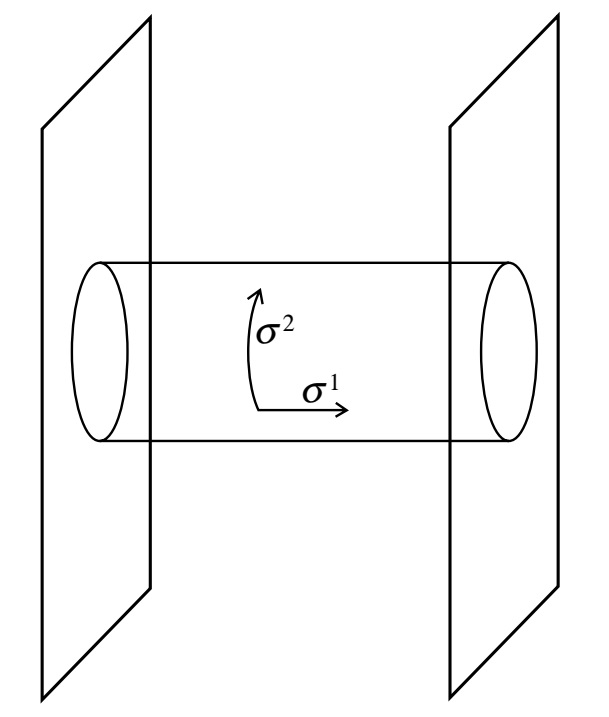
\includegraphics[width=0.6\textwidth]{figure/Fig8.5.jpg}\\
		\caption{Exchanging a closed string between two D-branes. Equivalently, this is the vacuum loop for an open string with endpoints attached to two D-branes.}\label{Fig8.5}
	\end{center}
\end{figure}

In section \ref{sec:7.4}, we calculated the annulus vacuum amplitude using an open string loop, but discovered closed string poles from the $t \rightarrow 0$ limit of the modular integral. 
This is exactly the pole we are interested in, but the simplest way to calculate the amplitude is to treat it as an open string loop. In fact, with a slight change, the previous result \eqref{7.4.1} can be used. 
The number of momentum integrals decreases from 26 to $p{+}1$, and similarly, $V_{26}$ becomes $V_{p+1}$ ; weights $h_{i}$ acquire an extra term $y^{2} / 4\pi^{2} \alpha^{\prime}$ due to stretched open strings; 
the Chan-Paton weight $n^{2}$ becomes 2 (since there are two directions for connecting the strings). 
Therefore we have:
\begin{align}
	\mathscr{A} &= \mi V_{p+1} \int_{0}^{\infty} \frac{\dif t}{t} (8 \pi^{2} \alpha^{\prime} t)^{-(p+1)/2} 
	\exp (-t y^{2} / 2 \pi \alpha^{\prime}) \eta(\mi t)^{-24}  \nonumber \\
	&= \frac{\mi V_{p+1}}{(8 \pi^{2} \alpha^{\prime})^{(p+1)/2}} 
	\int_{0}^{\infty} \dif t\: t^{(21-p)/2} \exp (-t y^{2} / 2 \pi \alpha^{\prime}) \nonumber \\
	& \qquad \qquad \qquad \qquad \qquad  \times[\exp (2 \pi/t)+24+\cdots] \:, \label{8.7.17}
\end{align}
where the asymptotic expansion is obtained by the method in section 7.4. 
The first term is tachyon exchange, thus it is a bosonic artifact. Integrating the second term gives:
\begin{align}
	\mathscr{A} &= \mi V_{p+1} \frac{24}{2^{12}}(4 \pi^{2} \alpha^{\prime})^{11-p} \pi^{(p-23)/2} 
	\Gamma\biggl(\frac{23-p}{2}\biggr)|y|^{p-23}  \nonumber \\
	&= \mi V_{p+1} \frac{24 \pi}{2^{10}}(4 \pi^{2} \alpha^{\prime})^{11-p} G_{25-p}(y) \:, \label{8.7.18}
\end{align}
where $G_{d}(y)$ is the Green function for a massless scalar in $d$ dimensions, the inverse of $-\nabla^{2}$. 
We now want to compare this with the field theory calculation of the same amplitude. Since antisymmetric tensors do not couple to D-branes, from the spacetime action \eqref{3.7.25}, the relevant terms are:
\begin{equation}
	\bm{S}=\frac{1}{2 \kappa^{2}} \int \dif^{26} X \: (-\tilde{G})^{1/2} 
	\biggl(\tilde{\bm{R}}-\frac{1}{6} \nabla_{\mu} \tilde{\Phi} \tilde{\nabla}^{\mu} \tilde{\Phi}\biggr) \:. \label{8.7.19}
\end{equation}
The tildes denote the Einstein metric.
Because this form of action decouples from the dilaton, it is convenient. The dilaton with tildes has been shifted such that its vacuum expectation value is zero. 
In terms of the same variable, the relevant term in the D-brane action \eqref{8.7.2} is:
\begin{equation}
	\bm{S}_{p} = -\tau_{p} \int \dif^{p+1} \xi \: \exp \biggl(\frac{p-11}{12} \tilde{\Phi}\biggr)
	(-\operatorname{det} \tilde{G}_{ab})^{1/2} \:. \label{8.7.20}
\end{equation}
We defined $\tau_{p}=T_{p} \me^{-\Phi_{0}}$; when the background value of the dilaton is $\Phi_{0}$, this is the true physical tension of the D$p$-brane.

The field theory diagram analogous to Figure 8.5 is the exchange of dilatons or gravitons between D-branes. To obtain the propagator, 
we expand the spacetime action up to second order in $h_{\mu\nu}=\tilde{G}_{\mu\nu}-\eta_{\mu\nu}$ and $\tilde{\Phi}$. 
Additionally, for gravity calculation, we need to choose a gauge. 
The simplest gauge for perturbative calculation is:
\begin{equation}
	F_{\nu} \equiv \partial^{\hat{\mu}} h_{\mu \nu}-\frac{1}{2} \partial_{\nu} h^{\hat{\mu}}{}_{\mu}=0 \:, \label{8.7.21}
\end{equation}
where the "hat" indicates using the flat metric $\eta^{\mu \nu}$ to raise and lower indices. 
Expanding the action to second order and adding the gauge fixing term $-F_{\nu} F^{\hat{\nu}} / 4\kappa^{2}$, 
the spacetime action becomes:
\begin{equation}
	\bm{S}=-\frac{1}{8 \kappa^{2}} \int \dif^{26} X \: \biggl( \partial_{\mu} h_{\nu \lambda} 
	\partial^{\hat{\mu}} h^{\hat{\nu} \hat{\lambda}}-\frac{1}{2} \partial_{\mu} h^{\hat{\nu}}{}_{\nu} 
	\partial^{\hat{\mu}} h^{\hat{\lambda}}{}_{\lambda}+\frac{2}{3} \partial_{\mu} \tilde{\Phi} \partial^{\hat{\mu}} \tilde{\Phi}\biggr) \:. \label{8.7.22}
\end{equation}
Observe the kinetic terms, yielding the momentum space propagator:
\begin{subequations} \label{8.7.23}
	\begin{align}
		\langle\tilde{\Phi} \tilde{\Phi}\rangle &=-\frac{(D-2) \mi \kappa^{2}}{4 k^{2}}  \:, \label{8.7.23a} \\
		\langle h_{\mu \nu} h_{\sigma \rho}\rangle &=-\frac{2 \mi \kappa^{2}}{k^{2}}
		\biggl(\eta_{\mu \sigma} \eta_{\nu \rho}+\eta_{\mu \rho} \eta_{\nu \sigma}-\frac{2}{D-2} \eta_{\mu \nu} \eta_{\sigma \rho}\biggr) \:. \label{8.7.23b}
	\end{align}
\end{subequations}
For later reference, we gave general $D$. Expanding around a general flat configuration, the D-brane action is:
\begin{equation}
	\bm{S}_{p}=-\tau_{p} \int \dif^{p+1} \xi \: \biggl(\frac{p-11}{12} \tilde{\Phi}-\frac{1}{2} h_{aa}\biggr) \:. \label{8.7.24}
\end{equation}
Note that $h_{\mu \nu}$ here is traced only over directions tangent to the D-brane; we have taken $\xi$ as Cartesian coordinates with metric $\delta_{ab}$. 
We can now read the Feynman diagram:
\begin{align}
	\mathscr{A} &= \frac{\mi \kappa^{2} \tau_{p}^{2}}{k_{\perp}^{2}} V_{p+1} 
	\left\{6\left[\frac{p-11}{12}\right]^{2}+\frac{1}{2}\left[2(p+1)-\frac{1}{12}(p+1)^{2}\right]\right\} \nonumber \\
	& =\frac{6 \mi \kappa^{2} \tau_{p}^{2}}{k_{\perp}^{2}} V_{p+1} \:. \label{8.7.25}
\end{align}
\begin{tcolorbox}
	\begin{remark}
		The above comes from $\langle S_p S_p \rangle$.
	\end{remark}	
\end{tcolorbox}
\noindent Comparison with \eqref{8.7.18} gives:
\begin{equation}
	\tau_{p}^{2} = \frac{\pi}{256 \kappa^{2}} (4 \pi^{2} \alpha^{\prime})^{11-p} \:. \label{8.7.26}
\end{equation}
This is consistent with the recurrence relation given by $T$-duality.

As an application, consider a state with $n$ 25-branes, which is identical to the ordinary $n$-valued Chan-Paton factor. 
Expanding the 25-brane action \eqref{8.7.12} to second order in the gauge field yields:
\begin{equation}
	\frac{\tau_{25}}{4}(2 \pi \alpha^{\prime})^{2} \operatorname{Tr}(F_{\mu \nu} F^{\mu \nu}) \:. \label{8.7.27}
\end{equation}
This relates the open string gauge coupling and closed string gravitational coupling. 
Using \eqref{6.5.14}, \eqref{6.5.16}, \eqref{6.6.15}, and \eqref{6.6.18}, 
we can write this as a relationship between the vertex operator normalizations $g_{\mathrm{c}}$ and $g_{\mathrm{o}}$:
\begin{equation}
	\frac{g_{\mathrm{o}}^{2}}{g_{\mathrm{c}}} = \frac{4 \pi \alpha^{\prime} g_{\mathrm{o}}^{\prime 2}}{\kappa}
	= 2^{18} \pi^{25 / 2} \alpha^{\prime 6} \:. \label{8.7.28}
\end{equation}
It has the correct form, with the square of the open string coupling being proportional to the closed string coupling, but now with a numerical coefficient. We decompose closed string poles from the torus via unitarity, or see Exercise 7.9.

\section{\texorpdfstring{$T$-duality of Unoriented Theories}{8.8 $T$-duality of Unoriented Theories}} \label{sec:8.8}
In unoriented string theory, the $R \rightarrow 0$ limit also yields interesting new physics. First consider the closed string theory. To form an unoriented theory, we impose $\Omega=+1$ on the states. 
Following the discussion in section 8.5, we can also think of this as gauging $\Omega$. In particular, the transition functions used to construct the worldsheet now reverse directions, and this produces an unoriented worldsheet.

The $T$-dual theory is obtained by replacing $X^{m}(z, \bar{z})=X_{L}^{m}(z)+X_{R}^{m}(\bar{z})$ with coordinates $X^{\prime m}(z, \bar{z})= X_{L}^{m}(z)-X_{R}^{m}(\bar{z})$. 
In the original description, we gauge worldsheet parity $\Omega$, whose action is:
\begin{equation}
	\Omega: X_{L}^{M}(z) \leftrightarrow X_{R}^{M}(z) \:. \label{8.8.1}
\end{equation}
In $T$-dual coordinates, this is:
\begin{subequations} \label{8.8.2}
	\begin{align}
		\Omega: \quad X^{\prime m}(z, \bar{z})  &\leftrightarrow-X^{\prime m}(\bar{z}, z) \:, \label{8.8.2a} \\
		X^{\mu}(z, \bar{z})  &\leftrightarrow X^{\mu}(\bar{z}, z) \:, \label{8.8.2b}
	\end{align}
\end{subequations}
as before, $m$ labels coordinates for which $T$-duality is taken, and $\mu$ labels coordinates for which $T$-duality is not taken. 
In the dual picture, symmetry \eqref{8.8.2} is thus the product of worldsheet parity transformation and spacetime inversion. 
We see that gauging worldsheet parity only produces an unoriented theory, while gauging inversion only produces an orbifold. The result of the combined projection is called an \emph{orientifold}.

An orientifold is very similar to an orbifold. Divide the string wave function into its interior and its center-of-mass $x^{m}$ dependent part, taking the interior wave function to be an eigenstate of $\Omega$. 
Then the projection onto $\Omega=+1$ indicates that the string wave function at $-x^{m}$ is the same as at $x^{m}$, differing only by a sign. 
For example, the components of the metric and antisymmetric tensor satisfy:
\begin{subequations} \label{8.8.3}
	\begin{align}
		G_{\mu \nu}(x^{\prime}) &= G_{\mu \nu}(x) \:, \quad  B_{\mu \nu}(x^{\prime})=-B_{\mu \nu}(x) \:, \label{8.8.3a} \\ 	
		G_{\mu n}(x^{\prime}) & =-G_{\mu n}(x) \:, \quad  B_{\mu n}(x^{\prime})=B_{\mu n}(x) 	\:, \label{8.8.3b} \\
		G_{m n}(x^{\prime}) &= G_{m n}(x) \:, \quad  B_{m n}(x^{\prime})=-B_{m n}(x) \:, \label{8.8.3c}
	\end{align}
\end{subequations}
where $(x^{\mu}, x^{m})^{\prime} = (x^{\mu},-x^{m})$. 
There is one negative sign for each of $m, n$ and another negative sign for $B_{M N}$; this is identical to an orbifold. 
In other words, the $T$-dual spacetime is the torus $T^{k}$ modulo the $\mathds{Z}_{2}$ reflection in $k$ compact dimensions, exactly the same as the construction of an orbifold. 
For example, if there is only one periodicity, the dual spacetime is the segment $0 \leq x^{25} \leq \pi R^{\prime}$, with orientifold fixed planes at the ends.

Note that when away from the orientifold fixed plane, the local physics is that of an oriented string theory. Unlike the original unoriented theory, where projection locally removes half of the states, 
here it relates the string wave function at any point to its value at the mirror point, as in \eqref{8.8.3}. 
One difference between orientifold and orbifold constructions is that the former has no direct analogue of twisted states because the Klein bottle has no modular transformation $\tau \rightarrow -1/\tau$. Examine Figure 8.6, which shows the torus and the Klein bottle. On the torus, the projection operator inserts a twist in the time-like direction in Figure 8.6a; rotating this figure by $90^{\circ}$, 
this becomes a twist in the spatial direction, implying the existence of twisted states in the spectrum. However, if the Klein bottle in Figure 8.6b is rotated by $90^{\circ}$, the time directions on relative sides cannot match. 
So there is no intermediate state interpretation in this channel. Thus it should be noted that the orientifold plane cannot be dynamical. Unlike the D-brane case, no string modes are tethered to the orientifold plane to represent its shape fluctuations. 
Our heuristic discussion—that gravitational waves force D-branes to oscillate here—does not apply to orientifold planes. Ultimately, the equivalence relation \eqref{8.8.3} becomes a boundary condition on fixed planes, causing incident waves to cancel with reflected waves. 
For D-branes, the reflected wave is a higher-order quantity of the string coupling.

\begin{figure}[!htbp]
	\begin{center}
		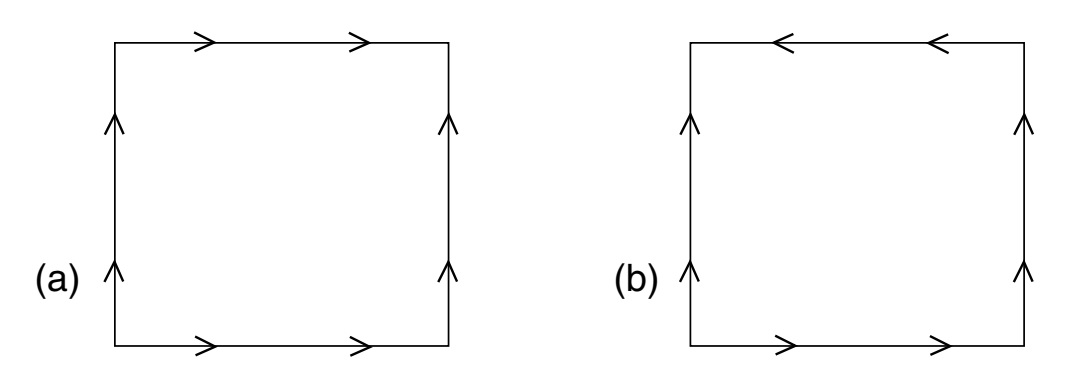
\includegraphics[width=0.8\textwidth]{figure/Fig8.6.jpg}
		\caption{Gluing opposite sides gives (a) a torus and (b) a Klein bottle.}\label{Fig8.6}
	\end{center}
\end{figure}

In drawing oriented strings, we use arrows to indicate directions. In unoriented theory, we can either omit the arrows or take a linear combination of the two directions. 
The latter picture is more consistent with the idea of gauging discrete symmetries and is more widespread: in an orientifold, parity operators must be accompanied by a spacetime transformation, so we cannot simply forget the arrows.

Although we introduced orientifold construction through $T$-duality, one can also examine orientifolds that are not $T$-duals of toroidal compactifications, combining worldsheet parity with various spacetime symmetries to gauge a group.

\subsection*{Open Strings}

In the case of open strings, the situation is similar. For simplicity, we only examine the case of one compact dimension. As before, there are orientifold fixed planes at 0 and $\pi R^{\prime}$. 
Introduce $SO(n)$ Chan-Paton factors (symplectic symmetry is similar), and a general Wilson line can be transformed into a diagonal form; when $n$ is even, the eigenvalues appear in pairs: 
\begin{equation}
	W = \operatorname{diag}\left(\me^{\mi \theta_{1}}, \me^{-\mi \theta_{1}}, \me^{\mi \theta_{2}}, \me^{-\mi \theta_{2}}, \cdots, 
	\me^{\mi \theta_{n/2}}, \me^{-\mi \theta_{n/2}}\right) \:. \label{8.8.4}
\end{equation}
Thus, in the dual picture, there are $\frac{1}{2} n$ D-branes in the segment $0 \leq X^{\prime 25} \leq \pi R^{\prime}$, and another $\frac{1}{2} n$ at mirror points. 
Strings can open between D-branes and mirrors, as shown in Figure \ref{Fig8.7}.
The general gauge group is $U(1)^{n/2}$. Similar to oriented theory, if $r$ D-branes coincide, then a $U(r)$ gauge group exists. 
If these $r$ D-branes are also on one of the fixed planes, then strings opening between one of these branes and its mirror brane are also massless. We would then have the correct spectrum of extra states to fill $SO(2r)$. 
If all branes are on an orientifold plane, the maximum $SO(n)$ is restored. 

\begin{figure}[!htbp]
	\begin{center}
		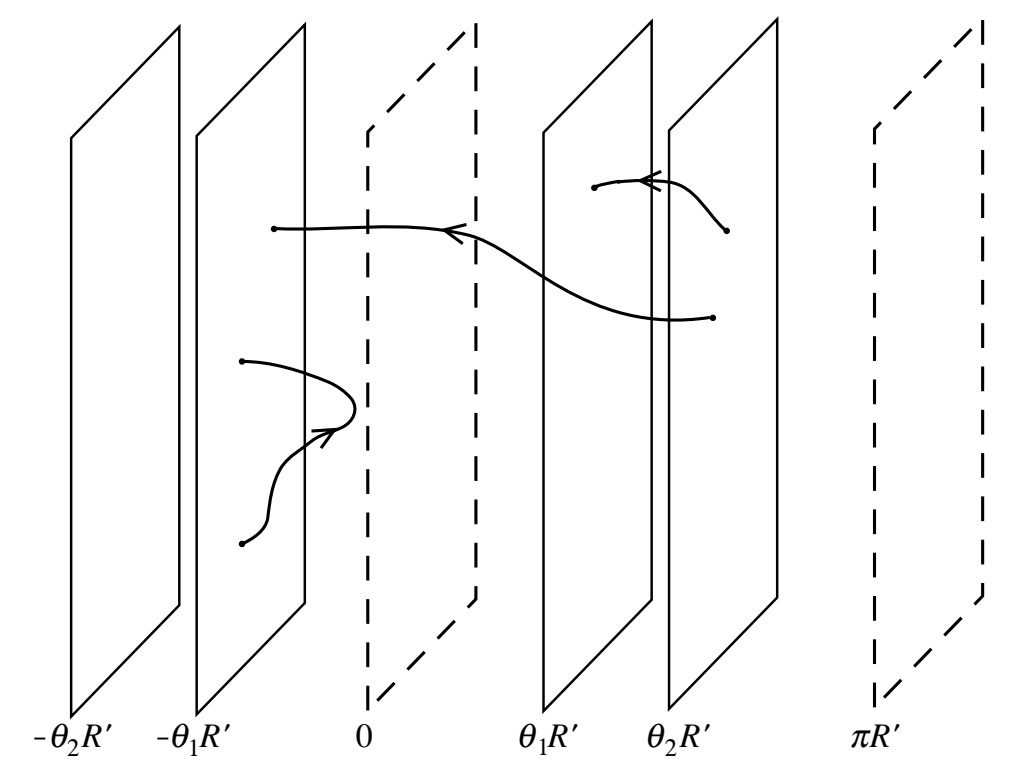
\includegraphics[width=0.6\textwidth]{figure/Fig8.7.jpg}
		\caption{Orientifold planes are at 0 and $\pi R^{\prime}$, D-branes are at $\theta_{1} R^{\prime}$ and $\theta_{2} R^{\prime}$, 
			and D-brane images are at $-\theta_{1} R^{\prime}$ and $-\theta_{2} R^{\prime}$. The effect of the twisting operator $\Omega$ on any string is a combination of spacetime reversal and reversal of oriented arrows.
		}\label{Fig8.7}
	\end{center}
\end{figure}

If $n$ is odd, the last eigenvalue of $W$ is $\pm 1$, causing it to be fixed on one of the two orientifold planes in the $T$-dual picture. 
Without mirrors, this is actually a half-D-brane. 
Additionally, if we examine the $n=2$ Wilson line $\operatorname{diag}(1,-1)$ (which is in $O(2)$ instead of $SO(2)$), what appears is not one D-brane and its image, but two half-D-branes.

As with D-branes, orientifold planes couple with the dilaton and metric. 
The amplitude is the same as in the previous section, except for replacing the annulus with Klein bottles and Möbius strips. 
In fact, we already performed relevant calculations in Chapter 7. There we found the total dilaton coupling cancels for $S O\left(2^{13}\right)$. 
In the $T$-dual picture, the total dilaton coupling of $2^{12}$ D-branes cancels (images are not included in the count). If we compactify $k=25-p$ dimensions, there will be $2^{k}$ fixed planes, 
whose coordinates are all combinations of 0 and $\pi R_{m}^{\prime}$. 
Thus the effective action of a single fixed plane is:
\begin{equation}
	2^{12-k} T_{p} \int \dif^{p+1} \xi \: \me^{-\Phi} (-\operatorname{det} G_{ab})^{1/2} \:, \label{8.8.5}
\end{equation}
where integration runs over fixed planes.

Although there is no direct analogue of twisted sectors in orientifolds, in some sense, twisted states are open strings. Since this analogy is not complete, we do not tend to emphasize it: 
gauging $\Omega$ itself does not introduce worldsheet boundaries. 
However, adding open strings to an orientifold theory to cancel the dilaton tadpole has certain physical significance. This cancellation will play an important role in superstrings.
	% \setcounter{section}{0}%Change the counter value of chapter
% %\numberwithin{equation}{chapter}%Equation counter belongs to section counter
% \numberwithin{equation}{section}%Equation counter belongs to section counter
% \numberwithin{figure}{section}%Figure counter belongs to section counter
% \setcounter{chapter}{8}

\chapter{\texorpdfstring{Higher order amplitudes}{9 Higher order amplitudes}} \label{cha:9}
In this chapter, we will discuss higher order amplitudes in string theory. The primary goal of the first half is to understand the finiteness and unitarity of string perturbation theory. After a detailed discussion of tree-level amplitudes, we will examine general amplitudes. 
Using the idea of factorization to relate higher order amplitudes to lower order ones, we will then discuss some ideas aimed at understanding all orders and even non-perturbative string theory.

%\section{\texorpdfstring{General tree-level amplitudes}{9.1 General tree-level amplitudes}}
\section{General tree-level amplitudes} \label{sec:9.1}

Chapter \ref{cha:6} preliminary examined the calculation of certain specific tree-level amplitudes.
It will be beneficial to open this chapter with a general analysis of a tree-level amplitude, as it will clarify some patterns that appear in higher order amplitudes. 
We will focus on oriented closed strings, as well as three-point and four-point amplitudes, which will illustrate some important features. The main topics are convergence and ``unitarity.'' The latter term is used in a broad sense. 
It refers both to the unitarity of the S-matrix $S S^{\dagger}=1$, and to the positive-definiteness of the Hilbert space. Of course, we already know from Chapter \ref{cha:4} that the BRST cohomology has a positive-definite inner product, 
which means we need to prove that the amplitudes follow BRST invariance: only BRST-invariant states can appear, and amplitudes of BRST-equivalent states are equal. 
For the latter, we gave a general discussion in Section \ref{sec:5.4}, but it can be explained more clearly here.

Before entering the general analysis, let us recall some useful results for calculations.
Suppose we have $d$ infinite flat dimensions, and the tachyon vertex operator is normalized to
\begin{equation}
	g_{\mathrm{c}, d} :\mathrel{\me^{\mi k \cdot X}}: \:. \label{9.1.1}
\end{equation}
For example, in the case of one dimension being toroidally compactified, we have $g_{\mathrm{c}, 25}=g_{\mathrm{c}}(2 \pi R)^{-1 / 2}$.
Then, for the matter part of a general OCQ vertex operator, the correct normalization can be fixed by the most singular term in the OPE:
\begin{equation}
	\mathscr{V}_{j}(k; z, \bar{z}) \overline{\mathscr{V}_{j^{\prime}}(k; 0,0)} = 
	\frac{g_{\mathrm{c}, d}^{2}}{z^{2} \bar{z}^{2}}+\ldots \:. \label{9.1.2}
\end{equation}
where the overline represents the Euclidean conjugate \eqref{6.7.28}. Since the vertex operator weight is (1,1), the singularity is $|z|^{-4}$.
Repeating the tachyon pole calculation \eqref{6.6.7} gives the normalization
\begin{align}
	& \me^{-2 \lambda} \Bigl\langle \tilde{c}(\bar{z}_{1}) c(z_{1}) \tilde{c}(\bar{z}_{2}) c(z_{2}) \tilde{c}(\bar{z}_{3}) 
	c(z_{3}) : \mathrel{\me^{\mi k \cdot X}(z, \bar{z})}:\Bigr\rangle \nonumber \\
	&\qquad \qquad \qquad \qquad =\frac{8 \pi \mi}{\alpha^{\prime} g_{\mathrm{c}, d}^{2}} 
	|z_{12} z_{13} z_{23}|^{2} (2 \pi)^{d} \delta^{d}(k) \:.
	\label{9.1.3}
\end{align}
\begin{tcolorbox}[breakable]
	\begin{remark}
		Conventions (as in Sections \ref{sec:6.2} and \ref{sec:6.6}). On the sphere the matter and ghost path integrals factorize. The ghost zero modes are saturated by three $c$ and three $\tilde c$, $\langle \tilde c c(z_1)\,\tilde c c(z_2)\,\tilde c c(z_3)\rangle = C^{\mathrm{g}}_{S_2}|z_{12}z_{13}z_{23}|^2$. The $X$ zero-mode integral gives the momentum $\delta$-function, together with a factor $\mi$ from the rotation of the $X^0$ contour, $\langle :\me^{\mi k\cdot X}:\rangle = \mi C^{X}_{S_2}(2\pi)^d\delta^d(k)$ (cf. \eqref{6.2.6}). Unitarity of the tachyon pole fixes $C_{S_2}=\me^{-2\lambda}C^X_{S_2}C^{\mathrm{g}}_{S_2}=8\pi/\alpha' g_{\mathrm{c}}^2$; with only $d$ noncompact dimensions the same argument holds with $g_{\mathrm{c}}\to g_{\mathrm{c},d}$. Then
		\begin{align*}
			&\me^{-2\lambda}\Bigl\langle \tilde c c(z_1)\,\tilde c c(z_2)\,\tilde c c(z_3)\,:\me^{\mi k\cdot X}:\Bigr\rangle\\
			&\qquad\eqs{1} \me^{-2\lambda}\bigl\langle \tilde c c\,\tilde c c\,\tilde c c\bigr\rangle_{\mathrm{g}}\,\bigl\langle :\me^{\mi k\cdot X}:\bigr\rangle_X
			\eqs{2} \me^{-2\lambda}C^{\mathrm{g}}_{S_2}|z_{12}z_{13}z_{23}|^2\cdot \mi C^X_{S_2}(2\pi)^d\delta^d(k)\\
			&\qquad\eqs{3} \frac{8\pi\mi}{\alpha' g_{\mathrm{c},d}^2}|z_{12}z_{13}z_{23}|^2(2\pi)^d\delta^d(k) .
		\end{align*}
		At (1) the ghost and matter CFTs decouple. At (2) the zero-mode results above were inserted. At (3) $C_{S_2}=8\pi/\alpha' g^2_{\mathrm{c},d}$.

		For one direction on a circle of radius $R$, the zero-mode integral over $x^{25}$ gives $\int_0^{2\pi R}\dif x^{25}\,\me^{\mi k_{25}x^{25}}=2\pi R\,\delta_{k_{25},0}$ in place of $2\pi\delta(k_{25})$. Hence
		\begin{gather*}
			\frac{(2\pi)^{26}\delta^{26}(k)}{g_{\mathrm{c}}^2}\;\longrightarrow\;\frac{2\pi R}{g_{\mathrm{c}}^2}(2\pi)^{25}\delta^{25}(k)\,\delta_{k_{25},0}
			\equiv\frac{(2\pi)^{25}\delta^{25}(k)\,\delta_{k_{25},0}}{g_{\mathrm{c},25}^2}\\
			\Longrightarrow\quad \boxed{g_{\mathrm{c},25}=g_{\mathrm{c}}(2\pi R)^{-1/2}} ,
		\end{gather*}
		which is the example quoted after \eqref{9.1.1}.
	\end{remark}
\end{tcolorbox}
All normalization constants in all S-matrices are written as $g_{\mathrm{c}, d}=\kappa_{d} / 2 \pi$.

\subsection*{Three-point amplitudes}

We first represent the tree-level amplitude in several useful forms. For a general tree-level three-point amplitude, the gauge-fixed expression of the string S-matrix \eqref{5.3.9} reduces to the path integral of three fixed vertex operators:
\begin{equation}
	S_{S_{2}}(1; 2; 3) = \me^{-2 \lambda} \Bigl\langle \hat{\mathscr{V}}_{1}^{\prime}(\infty, \infty) 
	\hat{\mathscr{V}}_{2}(1,1) \hat{\mathscr{V}}_{3}(0,0) \Bigr\rangle_{S_{2}} \:, \label{9.1.4}
\end{equation}
where the number $n$ is shorthand for the string momentum and state $(k_n, j_n)$.
The $\hat{}$ indicates that the vertex operator is in the fixed picture—that is, the integration over position does not introduce $b$ ghost insertions. 
As we discussed in Section \ref{sec:5.4}, this form naturally arises from the state-operator correspondence and, in the OCQ case, takes the following form:
\begin{equation}
	\hat{\mathscr{V}}_{j} = \tilde{c} c \mathscr{V}_{j} \:.
	\label{9.1.5}
\end{equation}
Using the results from Section \ref{sec:6.7}, the path integral on the sphere can be transformed into matrix elements; this amplitude can also be expressed as a matrix element or an operator product coefficient:
\begin{equation}
	S_{S_{2}}(1; 2; 3) = \me^{-2 \lambda}\lAngle\hat{\mathscr{V}}_{1}|\hat{\mathscr{V}}_{2}(1,1)|\hat{\mathscr{V}}_{3}\rangle
	= \me^{-2 \lambda} c_{123} \:. \label{9.1.6}
\end{equation}
This relates the amplitude in spacetime to the matrix element on the world-sheet, and further connects it to the operator product coefficients that encode the local properties of the CFT.

The first issue is the decoupling of BRST-null states, which ensures that BRST-equivalent states have the same amplitude.
Suppose $|\hat{\mathscr{V}}_{3}\rangle$ in the three-point amplitude is a null state:
\begin{equation}
	|\hat{\mathscr{V}}_{3}\rangle=Q_{\mathrm{B}}|\chi\rangle \:. \label{9.1.7}
\end{equation}
Then
\begin{align}
	\me^{2 \lambda} S_{S_{2}}(1; 2; 3) 
	&=  \lAngle \hat{\mathscr{V}}_{1} |
	[\hat{\mathscr{V}}_{2}(1,1), Q_{\mathrm{B}}] |\chi\rangle        
	+\lAngle \hat{\mathscr{V}}_{1} |
	Q_{\mathrm{B}} \hat{\mathscr{V}}_{2}(1,1) |\chi\rangle \nonumber \\
	&=0 \label{9.1.8}
\end{align}
Due to the BRST invariance of states 2 and 1, they are respectively zero. Similarly, if $\hat{\mathscr{V}}_{2}= \{Q_{\mathrm{B}}, \chi\}$ or 
$|\hat{\mathscr{V}}_{1}\rangle= Q_{\mathrm{B}}|\chi\rangle$, the amplitude is also zero. We have used the Hilbert space formalism here, 
but it is worth repeating the same discussion in the language of path integrals.
Suppose $\mathscr{V}_{3}$ is in the null space,
\begin{equation}
	\hat{\mathscr{V}}_{3}=Q_{\mathrm{B}} \cdot \mathscr{X}
\end{equation}
Expanding the contour integral on the sphere to move away from $\mathscr{X}$ until it becomes small loops around $\hat{\mathscr{V}}_{1}$ and $\hat{\mathscr{V}}_{2}$. 
They vanish due to BRST invariance, $Q_{\mathrm{B}} \cdot \hat{\mathscr{V}}_{1}=Q_{\mathrm{B}} \cdot \hat{\mathscr{V}}_{2}=0$.

Thus, to this order, the amplitude is well-defined in the physical Hilbert space, i.e., the BRST cohomology.
The decoupling of null gravitons corresponding to spacetime coordinate invariance is a special case of the decoupling of BRST-null states. 
Naturally, the question arises whether spacetime coordinate invariance is part of some larger symmetry. We will return to this question in Section \ref{sec:9.6}. 

We now examine the unitarity of the S-matrix
\begin{equation}
	\sum_{n} S_{mn} S_{pn}^{*} \questeq \delta_{mp} \:, \label{9.1.10}
\end{equation}
which is equivalent to probability conservation. Splitting the S-matrix into a constant term and a scattering term:
\begin{equation}
	S_{mn} = \delta_{mn} + \mi T_{mn} \:.
	\label{9.1.11}
\end{equation}
Then for the scattering matrix $T$, unitarity implies
\begin{equation}
	T_{mp} - T_{pm}^{*} = \mi \sum_{n} T_{mn} T_{pn}^{*} \:. \label{9.1.12}
\end{equation}
\begin{tcolorbox}[breakable]
	\begin{remark}
		Insert \eqref{9.1.11} into $SS^\dagger=1$:
		\begin{align*}
			1 &= (1+\mi T)(1-\mi T^\dagger)
			= 1+\mi\bigl(T-T^\dagger\bigr)+TT^\dagger ,\\
			&\Longrightarrow\quad
			T-T^\dagger \eqs{1} \mi\,TT^\dagger
			\quad\Longrightarrow\quad
			T_{mp}-T^{*}_{pm} \eqs{2} \mi\sum_n T_{mn}T^{*}_{pn} .
		\end{align*}
		At (1) the identity was cancelled and the equation multiplied by $-\mi$. At (2) the $mp$ matrix element was taken, using $(T^\dagger)_{mp}=T^{*}_{pm}$ and $(TT^\dagger)_{mp}=\sum_n T_{mn}(T^\dagger)_{np}=\sum_n T_{mn}T^{*}_{pn}$. The right side is quadratic in $T$, so at lowest order in the coupling (three-point, sphere) it vanishes and the condition is simply $T_{mp}=T^{*}_{pm}$.
	\end{remark}
\end{tcolorbox}

By definition, the $T$-matrix includes at least three particles, so for the three-particle amplitude on the sphere, the right side of \eqref{9.1.12} is zero.
Thus unitarity gives
\begin{equation}
	T_{S_{2}}(1; 2; 3) = T_{S_{2}}(-1; -2; -3)^{*} \:, \label{9.1.13}
\end{equation}
where the negative sign represents replacing the incoming vertex operator with the outgoing one. If the relationship between the incoming and outgoing vertex operators is
\begin{equation}
	\hat{\mathscr{V}}_{-i}=-\overline{\hat{\mathscr{V}}}_{i} \:. \label{9.1.14}
\end{equation}
Then \eqref{9.1.13} is satisfied.
This is a natural definition: conjugation transforms $\me^{\mi k \cdot X}$ into $\me^{-\mi k \cdot X}$, outgoing becomes incoming, and similarly for other quantum numbers. 
The negative sign is introduced to cancel the swap in the $\tilde{c} c$ order, which makes $\hat{\mathscr{V}}_{-i}$ simply the conjugation of all factors in the vertex operator that explicitly contain $\mi$.
Then the conjugation of the path integral gives
\begin{equation}
	\Bigl\langle \hat{\mathscr{V}}_{1}^{\prime}(\infty,\infty) \hat{\mathscr{V}}_{2}(1,1) \hat{\mathscr{V}}_{3}(0,0)\Bigr\rangle_{S_{2}}=-\Bigl\langle\hat{\mathscr{V}}_{-1}^{\prime}(\infty,\infty) \hat{\mathscr{V}}_{-2}(1,1) 
	\hat{\mathscr{V}}_{-3}(0,0)\Bigr\rangle_{S_{2}}^{*} \:, \label{9.1.15}
\end{equation}
\begin{tcolorbox}[breakable]
	\begin{remark}
		Conventions. For a vertex operator $A$, let $A^{\natural}$ denote $A$ with every explicit factor of $\mi$ complex conjugated and the order of all Grassmann factors kept. By the remark after \eqref{9.1.14}, $\hat{\mathscr V}_{-i}=\hat{\mathscr V}_i^{\natural}$: the explicit minus sign in \eqref{9.1.14} undoes the reversal $\tilde c c\to c\tilde c$ contained in the Euclidean conjugate. Write $\langle\cdots\rangle_{\mathrm E}$ for the sphere correlator before the $X^0$ contour is rotated. Its integrand is real, so $\langle A_1^\natural\cdots A_n^\natural\rangle_{\mathrm E}=\langle A_1\cdots A_n\rangle_{\mathrm E}^{*}$. The rotation of the $X^0$ zero mode multiplies every sphere correlator by one overall factor, $\langle\cdots\rangle=\mi\langle\cdots\rangle_{\mathrm E}$ (the $\mi$ of \eqref{6.2.6}). Then
		\begin{align*}
			\bigl\langle \hat{\mathscr V}'_1\hat{\mathscr V}_2\hat{\mathscr V}_3\bigr\rangle
			\eqs{1} \mi\bigl\langle \hat{\mathscr V}'_1\hat{\mathscr V}_2\hat{\mathscr V}_3\bigr\rangle_{\mathrm E}
			\eqs{2} \mi\bigl\langle \hat{\mathscr V}'_{-1}\hat{\mathscr V}_{-2}\hat{\mathscr V}_{-3}\bigr\rangle_{\mathrm E}^{*}
			\eqs{3} \mi\Bigl(-\mi\bigl\langle \hat{\mathscr V}'_{-1}\hat{\mathscr V}_{-2}\hat{\mathscr V}_{-3}\bigr\rangle\Bigr)^{*}
			= -\bigl\langle \hat{\mathscr V}'_{-1}\hat{\mathscr V}_{-2}\hat{\mathscr V}_{-3}\bigr\rangle^{*} .
		\end{align*}
		At (1) the overall $\mi$ was extracted. At (2) the reality of the Euclidean integrand was used, with $\hat{\mathscr V}_{-i}=\hat{\mathscr V}_i^\natural$. At (3) $\langle\cdots\rangle_{\mathrm E}=-\mi\langle\cdots\rangle$ was applied to the conjugated operators. This is \eqref{9.1.15}. For three particles $S=\mi T$, so with $\lambda$ real
		\begin{equation*}
			\mi T_{S_2}(1;2;3)=\me^{-2\lambda}\langle\cdots\rangle
			=-\bigl(\me^{-2\lambda}\langle\cdots\rangle_{-}\bigr)^{*}
			=-\bigl(\mi T_{S_2}(-1;-2;-3)\bigr)^{*}
			=\mi\,T_{S_2}(-1;-2;-3)^{*} ,
		\end{equation*}
		which is \eqref{9.1.13}. The same argument applies to any number of vertex operators, since only one overall $\mi$ appears: $S_{S_2}(1;\ldots;n)=-S_{S_2}(-1;\ldots;-n)^{*}$ wherever the $z$ integrals converge.
	\end{remark}
\end{tcolorbox}
which implies the unitary relation \eqref{9.1.13}. At first glance, this path integral is obviously real, and there should be no negative sign in \eqref{9.1.15}. 
However, we recall that this path integral must be defined through a specific analytic continuation, and the explicit result \eqref{6.2.6} thus acquires a total factor of $\mi$.
\subsection*{Four-point amplitudes and world-sheet duality}

The connected four-point amplitude is
\begin{equation}
	S_{S_{2}}(1; 2; 3; 4) = \me^{-2 \lambda} \int_{\mathds{C}} \dif^{2} z 
	\Bigl\langle \hat{\mathscr{V}}_{1}^{\prime}(\infty, \infty) \hat{\mathscr{V}}_{2}(1,1) \hat{\mathscr{V}}_{3}(0,0) 
	\mathscr{V}_{4}(z, \bar{z})\Bigr\rangle_{S_{2}} \:.
	\label{9.1.16}
\end{equation}
Writing this expectation value as a matrix element gives
\begin{equation}
	\lAngle\hat{\mathscr{V}}_{1}|\mathrm{T}[\hat{\mathscr{V}}_{2}(1,1) \mathscr{V}_{4}(z, \bar{z})]| 
	\hat{\mathscr{V}}_{3}\rangle \:. \label{9.1.17}
\end{equation}
For OCQ vertex operators, the ghost expectation value is constant. But to connect with the general case, it is more useful to move this ghost a bit. Using the contour discussion, the ghost insertion for the $\dif^{2} z$ integration can be written as
\begin{equation}
	\mathscr{V}_{4}(z, \bar{z})=(z \bar{z})^{-1}\bigl \{b_{0}, [\tilde{b}_{0}, \hat{\mathscr{V}}_{4}(z, \bar{z})]\bigr\} \:.
	\label{9.1.18}
\end{equation}
\begin{tcolorbox}[breakable]
	\begin{remark}
		With $b_0=\oint\frac{\dif w}{2\pi\mi}\,w\,b(w)$, the conjugate $\tilde b_0$, and $b(w)c(z)\sim 1/(w-z)$,
		\begin{equation*}
			\{b_0,c(z)\}=\oint_z\frac{\dif w}{2\pi\mi}\frac{w}{w-z}=z,\qquad \{\tilde b_0,\tilde c(\bar z)\}=\bar z,\qquad \{b_0,\tilde c\}=\{\tilde b_0,c\}=0 .
		\end{equation*}
		The operator $\hat{\mathscr V}_4=\tilde c c\,\mathscr V_4$ is Grassmann even and $\tilde b_0$ is odd, so the first bracket is a commutator and its result is odd:
		\begin{align*}
			[\tilde b_0,\tilde c c\,\mathscr V_4] &\eqs{1} \{\tilde b_0,\tilde c\}\,c\,\mathscr V_4-\tilde c\,\{\tilde b_0,c\}\,\mathscr V_4 \eqs{2} \bar z\,c\,\mathscr V_4 ,\\
			\{b_0,\bar z\,c\,\mathscr V_4\} &\eqs{3} \bar z\,\{b_0,c\}\,\mathscr V_4 = z\bar z\,\mathscr V_4 .
		\end{align*}
		At (1) the graded Leibniz rule was used; the matter factor commutes with the ghost modes. At (2) the anticommutators above were inserted. At (3) the same was done for $b_0$. Dividing by $z\bar z$ gives \eqref{9.1.18}.
	\end{remark}
\end{tcolorbox}
Using the above equation and the condition that $b_{0}$ and $\tilde{b}_{0}$ annihilate physical states \eqref{4.3.29}, the matrix element becomes
\begin{align}
	&\theta(1-|z|) \lAngle \hat{\mathscr{V}}_{1} |\hat{\mathscr{V}}_{2}(1,1) b_{0} \tilde{b}_{0} z^{L_{0}-1} \bar{z}^{\tilde{L}_{0}-1} 
	\hat{\mathscr{V}}_{4}(1,1)|
	\hat{\mathscr{V}}_{3}\rangle  \nonumber \\
	&\qquad + \theta(|z|-1) \lAngle\hat{\mathscr{V}}_{1}|\hat{\mathscr{V}}_{4}(1,1) b_{0} \tilde{b}_{0} z^{-L_{0}-1} 
	\bar{z}^{-\tilde{L}_{0}-1} \hat{\mathscr{V}}_{2}(1,1)|\hat{\mathscr{V}}_{3}\rangle \:.
	\label{9.1.19}
\end{align}
\begin{tcolorbox}[breakable]
	\begin{remark}
		Write $X(z,\bar z)\equiv\hat{\mathscr V}_4(z,\bar z)$. It has weight $(0,0)$ ($c$ has $-1$, $\mathscr V_4$ has $+1$), so the dilation generated by $L_0,\tilde L_0$ gives $X(z,\bar z)=z^{L_0}\bar z^{\tilde L_0}X(1,1)z^{-L_0}\bar z^{-\tilde L_0}$. Physical states obey $b_0|\hat{\mathscr V}\rangle=\tilde b_0|\hat{\mathscr V}\rangle=L_0|\hat{\mathscr V}\rangle=\tilde L_0|\hat{\mathscr V}\rangle=0$. The BPZ conjugates with $u=1/z$ map $b_0\to b_0$ and $L_0\to L_0$, so the same holds for $\lAngle\hat{\mathscr V}|$ acting to the right. Expanding the brackets,
		\begin{equation*}
			\{b_0,[\tilde b_0,X]\}=b_0\tilde b_0X-b_0X\tilde b_0+\tilde b_0Xb_0-X\tilde b_0b_0 .
		\end{equation*}
		For $|z|<1$ the radial ordering is $\hat{\mathscr V}_2(1,1)\mathscr V_4(z,\bar z)$:
		\begin{align*}
			\lAngle\hat{\mathscr V}_1|\hat{\mathscr V}_2(1,1)\mathscr V_4(z,\bar z)|\hat{\mathscr V}_3\rangle
			&\eqs{1} (z\bar z)^{-1}\lAngle\hat{\mathscr V}_1|\hat{\mathscr V}_2\,b_0\tilde b_0\,X(z,\bar z)|\hat{\mathscr V}_3\rangle\\
			&\eqs{2} (z\bar z)^{-1}\lAngle\hat{\mathscr V}_1|\hat{\mathscr V}_2\,b_0\tilde b_0\,z^{L_0}\bar z^{\tilde L_0}X(1,1)\,z^{-L_0}\bar z^{-\tilde L_0}|\hat{\mathscr V}_3\rangle\\
			&\eqs{3} \lAngle\hat{\mathscr V}_1|\hat{\mathscr V}_2\,b_0\tilde b_0\,z^{L_0-1}\bar z^{\tilde L_0-1}\hat{\mathscr V}_4(1,1)|\hat{\mathscr V}_3\rangle .
		\end{align*}
		At (1) \eqref{9.1.18} was used; the three terms with $b_0$ or $\tilde b_0$ on the far right annihilate $|\hat{\mathscr V}_3\rangle$. At (2) the dilation formula was used. At (3) $z^{-L_0}\bar z^{-\tilde L_0}|\hat{\mathscr V}_3\rangle=|\hat{\mathscr V}_3\rangle$. For $|z|>1$ the order is $\mathscr V_4(z,\bar z)\hat{\mathscr V}_2(1,1)$:
		\begin{align*}
			\lAngle\hat{\mathscr V}_1|\mathscr V_4(z,\bar z)\hat{\mathscr V}_2|\hat{\mathscr V}_3\rangle
			&\eqs{4} -(z\bar z)^{-1}\lAngle\hat{\mathscr V}_1|X(z,\bar z)\,\tilde b_0b_0\,\hat{\mathscr V}_2|\hat{\mathscr V}_3\rangle\\
			&= (z\bar z)^{-1}\lAngle\hat{\mathscr V}_1|z^{L_0}\bar z^{\tilde L_0}X(1,1)z^{-L_0}\bar z^{-\tilde L_0}\,b_0\tilde b_0\,\hat{\mathscr V}_2|\hat{\mathscr V}_3\rangle\\
			&\eqs{5} \lAngle\hat{\mathscr V}_1|\hat{\mathscr V}_4(1,1)\,b_0\tilde b_0\,z^{-L_0-1}\bar z^{-\tilde L_0-1}\hat{\mathscr V}_2(1,1)|\hat{\mathscr V}_3\rangle .
		\end{align*}
		At (4) the three terms with $b_0$ or $\tilde b_0$ on the far left vanish against $\lAngle\hat{\mathscr V}_1|$, and $-\tilde b_0b_0=b_0\tilde b_0$. At (5) $\lAngle\hat{\mathscr V}_1|z^{L_0}\bar z^{\tilde L_0}=\lAngle\hat{\mathscr V}_1|$, and $L_0$ commutes with $b_0,\tilde b_0$. Together these two results give \eqref{9.1.19}.

		For \eqref{9.1.20}, insert $1=\sum_{i,i'}|i\rangle\mathscr G^{ii'}\lAngle i'|$ to the right of the $z$-dependent factor, in a basis of $L_0,\tilde L_0$ eigenstates. For a closed-string state of momentum $k$ and levels $N,\tilde N$, $L_0=\frac{\alpha'}{4}k^2+N-1\equiv\frac{\alpha'}{4}(k^2+m^2)$ with $m^2=\frac{4}{\alpha'}(N-1)$, and similarly $\tilde m^2=\frac{4}{\alpha'}(\tilde N-1)$. Therefore $z^{L_0-1}\bar z^{\tilde L_0-1}|i\rangle=z^{\alpha'(k_i^2+m_i^2)/4-1}\bar z^{\alpha'(k_i^2+\tilde m_i^2)/4-1}|i\rangle$, which is the first line of \eqref{9.1.20}. The second line follows in the same way with $z\to z^{-1}$ in the exponents.
	\end{remark}
\end{tcolorbox}
We insert a complete basis of intermediate states into the matrix element:
\begin{align}
	&\quad \theta(1-|z|) \sum_{i, i^{\prime}} z^{\alpha^{\prime}(k_{i}^{2}+m_{i}^{2})/4 - 1} 
	\bar{z}^{\alpha^{\prime}(k_{i}^{2}+\tilde{m}_{i}^{2})/4 - 1} \nonumber  \\[-12pt] 
	& \qquad \qquad \qquad \qquad \times \lAngle \hat{\mathscr{V}}_{1}|\hat{\mathscr{V}}_{2}(1,1) b_{0} \tilde{b}_{0}|i\rangle 
	\mathscr{G}^{i i^{\prime}} \lAngle i^{\prime} |\hat{\mathscr{V}}_{4}(1,1)|
	\hat{\mathscr{V}}_{3}\rangle  \nonumber \\[5pt]
	&+ \theta(|z|-1) \sum_{i, i^{\prime}} z^{-\alpha^{\prime}(k_{i}^{2}+m_{i}^{2})/4 - 1} 
	\bar{z}^{-\alpha^{\prime}(k_{i}^{2}+\tilde{m}_{i}^{2})/4 - 1} \nonumber \\[-12pt] 
	& \qquad \qquad \qquad \qquad \times \lAngle \hat{\mathscr{V}}_{1} |\hat{\mathscr{V}}_{4}(1,1) b_{0} \tilde{b}_{0}|i\rangle 
	\mathscr{G}^{i i^{\prime}} \lAngle i^{\prime}|\hat{\mathscr{V}}_{2}(1,1)|\hat{\mathscr{V}}_{3}\rangle \:.
	\label{9.1.20}
\end{align}

In the latter form, the behavior of the integral as $z \rightarrow 0$ is obvious, and it is the same as the tachyon amplitude we studied in Chapter \ref{cha:6}. 
If $k_{i}^{2}+m_{i}^{2}$ and $k_{i}^{2}+\tilde{m}_{i}^{2}$ are positive for all $i$, i.e.,
\begin{equation}
	k_{i}^{2}=\left(k_{1}+k_{2}\right)^{2}>\frac{4}{\alpha^{\prime}} \:, \label{9.1.21}
\end{equation}
then the integral converges.
Elsewhere, it is defined as in \eqref{6.6.7}:
\begin{equation}
	\int_{|z|<1} \dif^{2} z \: z^{\alpha^{\prime}(k^{2}+m^{2})/4 - 1} \bar{z}^{\alpha^{\prime}(k^{2}+\tilde{m}^{2})/4 - 1}
	=\frac{8 \pi}{\alpha^{\prime}} \frac{\delta_{m^{2}, \tilde{m}^{2}}}{k^{2} + m^{2} - \mi \epsilon} \:.
	\label{9.1.22}
\end{equation}
\begin{tcolorbox}[breakable]
	\begin{remark}
		Let $a=\frac{\alpha'}{4}(k^2+m^2)$ and $\tilde a=\frac{\alpha'}{4}(k^2+\tilde m^2)$, so that $a-\tilde a=N-\tilde N\in\mathbb Z$. With $z=r\me^{\mi\theta}$ and the measure $\dif^2z=2\,\dif x\,\dif y=2r\,\dif r\,\dif\theta$,
		\begin{align*}
			\int_{|z|<1}\dif^2z\,z^{a-1}\bar z^{\tilde a-1}
			&\eqs{1} 2\int_0^1\dif r\,r^{a+\tilde a-1}\int_0^{2\pi}\dif\theta\,\me^{\mi(a-\tilde a)\theta}
			\eqs{2} 2\cdot2\pi\,\delta_{a,\tilde a}\,\frac{1}{a+\tilde a}\\
			&\eqs{3} \frac{2\pi}{a}\,\delta_{a,\tilde a}=\frac{8\pi}{\alpha'}\frac{\delta_{m^2,\tilde m^2}}{k^2+m^2} .
		\end{align*}
		At (1) $z^{a-1}\bar z^{\tilde a-1}=r^{a+\tilde a-2}\me^{\mi(a-\tilde a)\theta}$. At (2) the angular integral of an integer power of $\me^{\mi\theta}$ projects onto $a=\tilde a$, and the radial integral converges only for $\operatorname{Re}(a+\tilde a)>0$. At (3) $a=\tilde a$. The integral converges for every intermediate state if $a>0$ for the lightest one, the tachyon with $m^2=-4/\alpha'$, i.e.\ $k^2>4/\alpha'$, which is \eqref{9.1.21}. Elsewhere the right side is its analytic continuation. Continuing from large positive $k^2+m^2$ into the physical region past the pole defines the pole with the Feynman prescription $k^2+m^2-\mi\epsilon$.
	\end{remark}
\end{tcolorbox}
This can be thought of as an analytic continuation from large positive $m^{2}$ values. Similarly, the integral for $z \rightarrow \infty$ converges for $(k_{1}+k_{4})^{2}>4 / \alpha^{\prime}$, 
and is defined elsewhere by analytic continuation. If studying the limit $z \rightarrow 1$, \eqref{9.1.20} is useless. Instead, use the symmetry of the amplitude to swap vertex operators 2 and 3.
Then the integral for $z \rightarrow 1$ is defined by analytic continuation from the convergence region $(k_{1}+k_{3})^{2}>4 / \alpha^{\prime} $.

After integrating \eqref{9.1.20} as in \eqref{9.1.22}, the amplitude is expressed as a series of $s$ and $u$ poles. We know from Chapter \ref{cha:6} that this amplitude also has $t$ poles, but this is not obvious: 
they come from the divergence of the infinite sum.
A similar open string amplitude $I(s, t)$ has $s$ and $t$ poles, but it can be written as an infinite sum of $s$ or $t$. 
This property is called \emph{duality}, or \emph{world-sheet duality}. We can think of it as arising from cutting the world-sheet along different curves, which represents summing over intermediate states in different ways. 
Another example is summing over open string states to give closed string poles on the cylinder.

\subsection*{Four-point amplitude unitarity}

We now verify that four-point amplitudes are equal for equivalent states. Let $|\hat{\mathscr{V}}_{3}\rangle=Q_{\mathrm{B}}|\chi\rangle$ be a null state.
Using \eqref{9.1.19}, we swap $Q_{\mathrm{B}}$ to the left until it annihilates $\lAngle\hat{\mathscr{V}}_{1}|$. 
The BRST operator commutes with $L_{0}, \tilde{L}_{0}$ and the vertex operators, but does not commute with $b_{0}$ and $\tilde{b}_{0}$.
Non-zero commutators include
\begin{equation}
	\Bigl[b_{0} \tilde{b}_{0} z^{\pm L_{0}-1} \bar{z}^{\pm \tilde{L}_{0}-1}, Q_{\mathrm{B}}\Bigr] = 
	\pm b_{0} \partial_{\bar{z}}\Bigl(z^{\pm L_{0}-1} \bar{z}^{\pm \tilde{L}_{0}}\Bigr) \mp 
	\tilde{b}_{0} \partial_{z}\Bigl(z^{\pm L_{0}} \bar{z}^{\pm \tilde{L}_{0}-1}\Bigr) \:.
	\label{9.1.23}
\end{equation}
\begin{tcolorbox}[breakable]
	\begin{remark}
		The inputs are $\{Q_{\mathrm B},b_0\}=L_0$, $\{Q_{\mathrm B},\tilde b_0\}=\tilde L_0$, and $[Q_{\mathrm B},L_0]=[Q_{\mathrm B},\tilde L_0]=0$, so any function $F$ of $L_0,\tilde L_0$ commutes with $Q_{\mathrm B}$. Since $b_0\tilde b_0$ is even,
		\begin{align*}
			b_0\tilde b_0\,Q_{\mathrm B}
			&\eqs{1} b_0\bigl(\tilde L_0-Q_{\mathrm B}\tilde b_0\bigr)
			\eqs{1} b_0\tilde L_0-\bigl(L_0-Q_{\mathrm B}b_0\bigr)\tilde b_0
			=Q_{\mathrm B}\,b_0\tilde b_0+b_0\tilde L_0-\tilde b_0L_0 ,\\
			\bigl[b_0\tilde b_0F,Q_{\mathrm B}\bigr]
			&\eqs{2} \bigl(b_0\tilde L_0-\tilde b_0L_0\bigr)F .
		\end{align*}
		At (1) $\tilde b_0Q_{\mathrm B}=\tilde L_0-Q_{\mathrm B}\tilde b_0$ and then $b_0Q_{\mathrm B}=L_0-Q_{\mathrm B}b_0$ were used. At (2) $F$ was moved through $Q_{\mathrm B}$. Now take $F=z^{\pm L_0-1}\bar z^{\pm\tilde L_0-1}$ and use $\pm\tilde L_0\bar z^{\pm\tilde L_0-1}=\partial_{\bar z}\bar z^{\pm\tilde L_0}$ and $\pm L_0z^{\pm L_0-1}=\partial_zz^{\pm L_0}$:
		\begin{equation*}
			\bigl(b_0\tilde L_0-\tilde b_0L_0\bigr)z^{\pm L_0-1}\bar z^{\pm\tilde L_0-1}
			=\pm b_0\,\partial_{\bar z}\bigl(z^{\pm L_0-1}\bar z^{\pm\tilde L_0}\bigr)\mp\tilde b_0\,\partial_z\bigl(z^{\pm L_0}\bar z^{\pm\tilde L_0-1}\bigr) ,
		\end{equation*}
		which is \eqref{9.1.23}. Inside $\int\dif^2z$ both terms are total derivatives, so the only possible contributions come from the boundaries $z\to0,1,\infty$ of the moduli space.
	\end{remark}
\end{tcolorbox}
They are total derivatives, illustrating the general principle \eqref{5.4.6}: the coupling of a null state is proportional to the derivative on the moduli space. We saw such an example for the massless vertex operators in Section \ref{sec:6.6}. 
In that example, the integral vanished due to the cancellation of the propagator. The integral at $z \rightarrow 0$ is obtained by analytic continuation from large positive $(k_{1} + k_{2})^{2}$. 
The surface term is identically zero there, so it is zero everywhere by analyticity. The same discussion applies to other limits of the moduli space.
For the four-point amplitude on the sphere, the unitarity condition is
\begin{align}
	& T_{S_{2}}(1; 2; 3; 4) - T_{S_{2}}(-1; -2; -3; -4)^{*} \nonumber \\
	& \quad = \mi \sum_{j_{5}} \int \frac{\dif^{d-1} \mathbf{k}_{5}}{2 E_{5}(2 \pi)^{d-1}} T_{S_{2}}(1; 2; 5) T_{S_{2}}(-5; 3; 4)
	+ \text{2 permutations} \nonumber \\
	& \quad = -\mi \me^{-4 \lambda} \sum_{j_{5}} \int \frac{\dif^{d-1} \mathbf{k}_{5}}{2 E_{5}(2 \pi)^{d-1}}
	\lAngle\hat{\mathscr{V}}_{1} |\hat{\mathscr{V}}_{2}(1,1)|
	\hat{\mathscr{V}}_{5}\rangle 
	\lAngle\hat{\mathscr{V}}_{-5}|\hat{\mathscr{V}}_{3}(1,1)| \hat{\mathscr{V}}_{4}\rangle  \nonumber \\
	& \qquad + \text{2 permutations} \: .
	\label{9.1.24}
\end{align}
\begin{tcolorbox}[breakable]
	\begin{remark}
		All momenta are counted as incoming. Crossing turns $T_{mp}$, with $m=\{1,2\}$ incoming and $p$ outgoing, into $T_{S_2}(1;2;3;4)$, where $3,4$ are the conjugates of the particles in $p$. The first line is \eqref{9.1.12}, with $T_{pm}^{*}=T_{S_2}(-3;-4;-1;-2)^{*}=T_{S_2}(-1;-2;-3;-4)^{*}$ by symmetry of the amplitude. At this order the intermediate states $n$ are single on-shell strings, and a one-particle sum in relativistic normalization is $\sum_n\to\sum_{j_5}\int\frac{\dif^{d-1}\mathbf k_5}{2E_5(2\pi)^{d-1}}$, after the overall momentum $\delta$-function is stripped. Then
		\begin{align*}
			\mi\sum_nT_{mn}T^{*}_{pn}
			&\eqs{1} \mi\sum_{j_5}\int\frac{\dif^{d-1}\mathbf k_5}{2E_5(2\pi)^{d-1}}\,T_{S_2}(1;2;5)\,T_{S_2}(-5;3;4)\\
			&\eqs{2} \mi\,(-\mi)^2\me^{-4\lambda}\sum_{j_5}\int\frac{\dif^{d-1}\mathbf k_5}{2E_5(2\pi)^{d-1}}
			\lAngle\hat{\mathscr V}_1|\hat{\mathscr V}_2(1,1)|\hat{\mathscr V}_5\rangle\lAngle\hat{\mathscr V}_{-5}|\hat{\mathscr V}_3(1,1)|\hat{\mathscr V}_4\rangle ,
		\end{align*}
		which is the last line, since $\mi(-\mi)^2=-\mi$. At (1) the reality condition \eqref{9.1.13} was used, $T_{pn}^{*}=T_{S_2}(-5;3;4)$. At (2) each three-point amplitude was converted by \eqref{9.1.6} with $S=\mi T$, i.e.\ $T_{S_2}(1;2;3)=-\mi\,\me^{-2\lambda}\lAngle\hat{\mathscr V}_1|\hat{\mathscr V}_2(1,1)|\hat{\mathscr V}_3\rangle$. The two permutations are the other pairings, $13$--$24$ and $14$--$23$.
	\end{remark}
\end{tcolorbox}
Intermediate particles are on-shell, and the sum over $j_{5}$ covers all ways to split 1234 into two pairs: 12-34, 13-24, and 14-23.

\eqref{9.1.24} is what we want to prove. Using the real condition \eqref{9.1.13} in the matrix element \eqref{9.1.20}, the left side of \eqref{9.1.24} is zero within the $z$ integration convergence region.
The non-zero part comes from the $\mi \epsilon$ introduced during analytic continuation:
\begin{equation}
	\frac{1}{k^{2} + m^{2} - \mi \epsilon} - \frac{1}{k^{2}+m^{2}+ \mi \epsilon}=2 \pi \mi \delta(k^{2}+m^{2}) \:.
	\label{9.1.25}
\end{equation}
Therefore
\begin{align}
	& T_{S_{2}}(1; 2; 3; 4) - T_{S_{2}}(-1; -2; -3; -4)^{*} \nonumber \\
	&\quad =\frac{16 \pi^{2} \mi}{\alpha^{\prime} \me^{2 \lambda}} 
	\sum_{i, i^{\prime}} \delta_{m_{i}^{2}, \tilde{m}_{i}^{2}} \delta(k_{i}^{2}+m_{i}^{2})
	\lAngle\hat{\mathscr{V}}_{1}|\hat{\mathscr{V}}_{2}(1,1) b_{0} \tilde{b}_{0}|
	i\rAngle \mathscr{G}^{i i^{\prime}} 
	\lAngle i^{\prime} |\hat{\mathscr{V}}_{3}(1,1)| \hat{\mathscr{V}}_{4}\rangle \nonumber \\
	&\qquad +\text{2 permutations.} \label{9.1.26}
\end{align}
\begin{tcolorbox}[breakable]
	\begin{remark}
		First, \eqref{9.1.25}: for real $x$,
		\begin{equation*}
			\frac{1}{x-\mi\epsilon}-\frac{1}{x+\mi\epsilon}=\frac{2\mi\epsilon}{x^2+\epsilon^2}\;\xrightarrow{\;\epsilon\to0\;}\;2\pi\mi\,\delta(x),
		\end{equation*}
		since $\epsilon/(x^2+\epsilon^2)$ has unit area $\pi$ and shrinks to $x=0$.

		Now let $F(x)$, with $x=k_i^2+m_i^2$, be the analytic function that the $z$ integral defines in its convergence region. The remark after \eqref{9.1.15} gives $S=-S_{-}^{*}$ there, hence $T=-\mi S$ equals $T_{-}^{*}$. Both sides are analytic, so the identity continues everywhere. The physical amplitudes are boundary values: $T=F(x-\mi\epsilon)$, and complex conjugation reverses the prescription, $T_{-}^{*}=F(x+\mi\epsilon)$. The difference is therefore the discontinuity across the poles, which comes from the $|z|<1$ region of \eqref{9.1.20} integrated by \eqref{9.1.22} (with $\hat{\mathscr V}_{3}(1,1)|\hat{\mathscr V}_4\rangle$ and $\hat{\mathscr V}_4(1,1)|\hat{\mathscr V}_3\rangle$ equal by the M\"obius map $z\to1-z$). Writing $M_{ii'}=\lAngle\hat{\mathscr V}_1|\hat{\mathscr V}_2 b_0\tilde b_0|i\rangle\mathscr G^{ii'}\lAngle i'|\hat{\mathscr V}_3(1,1)|\hat{\mathscr V}_4\rangle$,
		\begin{align*}
			&T_{S_2}(1;2;3;4)-T_{S_2}(-1;-2;-3;-4)^{*}\\
			&\qquad\eqs{1} -\mi\,\me^{-2\lambda}\frac{8\pi}{\alpha'}\sum_{i,i'}\delta_{m_i^2,\tilde m_i^2}M_{ii'}\Bigl[\frac{1}{x_i-\mi\epsilon}-\frac{1}{x_i+\mi\epsilon}\Bigr]+\cdots\\
			&\qquad\eqs{2} -\mi\cdot2\pi\mi\,\frac{8\pi}{\alpha'}\me^{-2\lambda}\sum_{i,i'}\delta_{m_i^2,\tilde m_i^2}\delta(x_i)M_{ii'}+\cdots\\
			&\qquad=\boxed{\frac{16\pi^2}{\alpha'\me^{2\lambda}}}\sum_{i,i'}\delta_{m_i^2,\tilde m_i^2}\delta(k_i^2+m_i^2)M_{ii'}+\cdots .
		\end{align*}
		At (1) $T=-\mi S$ with $S=\me^{-2\lambda}\int\dif^2z\langle\cdots\rangle$, the pole part of the $|z|<1$ region was taken from \eqref{9.1.22}, and the dots are the two other channels. At (2) \eqref{9.1.25} was used. Note that $-\mi\cdot2\pi\mi=2\pi$ is real, so this chain gives the prefactor $16\pi^2/\alpha'\me^{2\lambda}$ without the explicit $\mi$ printed in \eqref{9.1.26}. The next box shows that this real prefactor, combined with \eqref{9.1.28}, reproduces exactly the $-\mi\me^{-4\lambda}$ of \eqref{9.1.24}. With the extra $\mi$ the two sides would differ by a factor $\mi$, so the $\mi$ in \eqref{9.1.26} should be dropped.
	\end{remark}
\end{tcolorbox}
This is very close to the desired unitarity relation \ref{9.1.24}, requiring a bit of manipulation to complete the result. The index $i$ in the sum \eqref{9.1.26} runs over the complete basis of string states, marking internal states and momenta:
\begin{equation}
	i \leftrightarrow(j, k) \:.
	\label{9.1.27}
\end{equation}
The $\delta$-function introduced in \eqref{9.1.26} along with the $b_{0} \tilde{b}_{0}$ factor projects onto the space $\hat{\mathscr{H}}$ annihilated by $L_{0}, \tilde{L}_{0}, b_{0}$ and $\tilde{b}_{0}$, which was introduced in the discussion of BRST cohomology. Therefore
\begin{align}
	&\sum_{i, i^{\prime}} \delta_{m_{i}^{2}, \tilde{m}_{i}}^{2} \delta(k_{i}^{2}+m_{i}^{2}) b_{0} \tilde{b}_{0}
	|i\rangle \mathscr{G}^{i i^{\prime}}\lAngle i^{\prime}|
	\nonumber  \\
	&\qquad =\delta_{L_{0}, \tilde{L}_{0}} \delta(4 L_{0} / \alpha^{\prime}) b_{0} \tilde{b}_{0}  \nonumber \\
	&\qquad =-\frac{\mi \alpha^{\prime}}{16 \pi^{2} \me^{2 \lambda}} \int \frac{\dif^{d-1} \mathbf{k}}{2 E(2 \pi)^{d-1}} 
	\sum_{j \in \hat{\mathscr{H}} \atop k^{0}=\pm \omega_{k}}
	|\hat{\mathscr{V}}_{j}(k)\rangle \lAngle\overline{\hat{\mathscr{V}}_{j}(k)}|
	\:. \label{9.1.28}
\end{align}
The normalization of the basis $|\mathscr{V}_{j}(k)\rangle$ can be derived from the OPE \eqref{9.1.2} and the expectation value \eqref{9.1.3}, which gives
\begin{equation}
	\lAngle\overline{\hat{\mathscr{V}}_{j}(k)}|\tilde{c}_{0} c_{0}| \hat{\mathscr{V}}_{j^{\prime}}(k^{\prime})\rangle = 
	\frac{8 \pi \mi \me^{2 \lambda}}{\alpha^{\prime}} \delta_{j j^{\prime}}(2 \pi)^{d} \delta^{d}(k-k^{\prime}) \:. \label{9.1.29}
\end{equation}
\begin{tcolorbox}[breakable]
	\begin{remark}
		Conventions. In \eqref{9.1.28} and \eqref{9.1.29} the bra $\lAngle\overline{\hat{\mathscr V}_j(k)}|$ is taken with its ghost factor in the order $\tilde c c$ used in \eqref{9.1.3}. By \eqref{9.1.14} and the remark after \eqref{9.1.15}, this is the bra of $\hat{\mathscr V}_{-j}(k)=\tilde c c\,\overline{\mathscr V_j(k)}$. This is the convention in which the printed sign of \eqref{9.1.29} follows from \eqref{9.1.3}. Reversing the ghost order flips the signs of \eqref{9.1.28} and \eqref{9.1.29} together and leaves every physical statement unchanged.

		\emph{Normalization \eqref{9.1.29}.} Between the ghost ground states only the zero modes of $c(1)=\sum_n c_n$ and $\tilde c(1)$ contribute, so $\lAngle\hat{\mathscr V}_{-j}|\tilde c_0c_0|\hat{\mathscr V}_{j'}\rangle=\lim_{z_1\to\infty}\langle\hat{\mathscr V}_{-j}(z_1)\,\tilde c c(1)\,\hat{\mathscr V}_{j'}(0)\rangle$; no conformal factor appears because $\hat{\mathscr V}$ has weight $(0,0)$. The matter two-point function is fixed by the OPE \eqref{9.1.2}, $\overline{\mathscr V_j}(z_1)\mathscr V_{j'}(z_3)\to\delta_{jj'}g_{\mathrm c,d}^2|z_{13}|^{-4}\times(\text{identity with momentum }k'-k)$. Then
		\begin{align*}
			\me^{-2\lambda}\langle\hat{\mathscr V}_{-j}(z_1)\,\tilde c c(z_2)\,\hat{\mathscr V}_{j'}(z_3)\rangle
			&\eqs{1} \delta_{jj'}\frac{g_{\mathrm c,d}^2}{|z_{13}|^4}\cdot\frac{8\pi\mi}{\alpha' g_{\mathrm c,d}^2}|z_{12}z_{13}z_{23}|^2(2\pi)^d\delta^d(k'-k)\\
			&= \frac{8\pi\mi}{\alpha'}\,\delta_{jj'}\frac{|z_{12}|^2|z_{23}|^2}{|z_{13}|^2}(2\pi)^d\delta^d(k-k')\\
			&\xrightarrow{\;z_1\to\infty,\ z_2=1,\ z_3=0\;}\;\frac{8\pi\mi}{\alpha'}\delta_{jj'}(2\pi)^d\delta^d(k-k') .
		\end{align*}
		At (1) \eqref{9.1.3} was used for the ghosts and the leftover exponential. Multiplying by $\me^{2\lambda}$ gives \eqref{9.1.29}. Call this normalization $\mathcal N=8\pi\mi\me^{2\lambda}/\alpha'$.

		\emph{Projector \eqref{9.1.28}.} For each $|v\rangle\equiv|\hat{\mathscr V}_j(k)\rangle\in\hat{\mathscr H}$ the states $|v\rangle$ and $|w\rangle=\tilde c_0c_0|v\rangle$ both appear in the complete basis. The only nonvanishing pairing of $|w\rangle$ is with the bra $\lAngle v_-|\equiv\lAngle\hat{\mathscr V}_{-j}(k)|$, namely $\mathcal N$ times the momentum $\delta$-function. Completeness therefore contains $|w\rangle\lAngle v_-|/\mathcal N$. Moreover
		\begin{gather*}
			b_0\tilde b_0\tilde c_0c_0|v\rangle\eqs{2} b_0c_0|v\rangle\eqs{2}|v\rangle ,\\
			b_0\tilde b_0|v\rangle=b_0\tilde b_0c_0|v\rangle=b_0\tilde b_0\tilde c_0|v\rangle=0 ,
		\end{gather*}
		where (2) uses $\tilde b_0\tilde c_0=1-\tilde c_0\tilde b_0$, $b_0c_0=1-c_0b_0$, and $b_0|v\rangle=\tilde b_0|v\rangle=0$. So $b_0\tilde b_0$ keeps exactly the $|w\rangle$ terms and converts them into $|v\rangle$. With $\sum_i\to\sum_j\int\frac{\dif^dk}{(2\pi)^d}$ and $\delta(k^2+m^2)=\sum_{k^0=\pm\omega_k}\delta(k^0\mp\omega_k)/2\omega_k$,
		\begin{align*}
			\sum_{i,i'}\delta_{m_i^2,\tilde m_i^2}\delta(k_i^2+m_i^2)\,b_0\tilde b_0|i\rangle\mathscr G^{ii'}\lAngle i'|
			&\eqs{3} \frac{1}{\mathcal N}\sum_{j\in\hat{\mathscr H}}\int\frac{\dif^dk}{(2\pi)^d}\,\delta(k^2+m^2)\,|\hat{\mathscr V}_j(k)\rangle\lAngle\hat{\mathscr V}_{-j}(k)|\\
			&\eqs{4} \frac{\alpha'}{8\pi\mi\,\me^{2\lambda}}\cdot\frac{1}{2\pi}\int\frac{\dif^{d-1}\mathbf k}{2E(2\pi)^{d-1}}\sum_{j,\ \pm}|\hat{\mathscr V}_j(k)\rangle\lAngle\hat{\mathscr V}_{-j}(k)|\\
			&= -\frac{\mi\alpha'}{16\pi^2\me^{2\lambda}}\int\frac{\dif^{d-1}\mathbf k}{2E(2\pi)^{d-1}}\sum_{j,\ \pm}|\hat{\mathscr V}_j(k)\rangle\lAngle\hat{\mathscr V}_{-j}(k)| ,
		\end{align*}
		At (3) the $b_0\tilde b_0$ projection just described was applied; the constraint $L_0=\tilde L_0=0$ on $\hat{\mathscr H}$ is the $\delta$-function together with $\delta_{m^2,\tilde m^2}$. At (4) the $k^0$ integral was done, $\int\dif k^0/2\pi$ against $\delta(k^2+m^2)$ giving $1/(2\pi\cdot2E)$, with $\pm$ labelling $k^0=\pm\omega_k$. This is \eqref{9.1.28}.

		\emph{Check of \eqref{9.1.24}.} Insert this into \eqref{9.1.26} with the real prefactor found in the previous box:
		\begin{equation*}
			\frac{16\pi^2}{\alpha'\me^{2\lambda}}\cdot\Bigl(-\frac{\mi\alpha'}{16\pi^2\me^{2\lambda}}\Bigr)=-\mi\,\me^{-4\lambda},
		\end{equation*}
		so the discontinuity becomes $-\mi\me^{-4\lambda}\int\frac{\dif^{d-1}\mathbf k}{2E(2\pi)^{d-1}}\sum_j\lAngle\hat{\mathscr V}_1|\hat{\mathscr V}_2|\hat{\mathscr V}_j(k)\rangle\lAngle\hat{\mathscr V}_{-j}(k)|\hat{\mathscr V}_3|\hat{\mathscr V}_4\rangle$. Only one sign of $k^0$ is allowed by momentum conservation in each channel. This is the right side of \eqref{9.1.24} with $5=(j,k)$, except that $j$ still runs over all of $\hat{\mathscr H}$ rather than over the BRST cohomology. That gap is closed below by \eqref{9.1.31}.
	\end{remark}
\end{tcolorbox}

Using \eqref{9.1.28}, one can see that the form, normalization, and unitarity condition of \eqref{9.1.26} are completely consistent with \eqref{9.1.24}, leaving only one gap.
The sum in the unitarity relation only runs over the physical state space, i.e., the BRST cohomology, whereas the final sum in \eqref{9.1.28} runs over a complete basis of $\hat{\mathscr{H}}$. 
We now prove these sums are equal. Consider the following basis of $\hat{\mathscr{H}}$. 
First, take a complete basis of ``unphysical states'' $|a\rangle_{\mathrm{U}}$, i.e., their linear combinations are not annihilated by $Q_{\mathrm{B}}$.
Second, take a complete basis of BRST-invariant states $|b\rangle_{\mathrm{P}}$, which are linearly independent, i.e., their linear combinations are not null states.
Finally, take the BRST-null states $|a\rangle_{\mathrm{N}}=Q_{\mathrm{B}}|a\rangle_{\mathrm{U}}$, and the entire basis is complete.
Define operators $\mathscr{P}$ and $\mathscr{U}$:
\begin{subequations} \label{9.1.30}
	\begin{align}
		&\mathscr{P}|b\rangle_{\mathrm{P}} = |b\rangle_{\mathrm{P}}, \quad \mathscr{P}|a\rangle_{\mathrm{U}}=0, \quad 
		\mathscr{P}|a\rangle_{\mathrm{N}} = 0 \:;
		\label{9.1.30a} \\
		&\mathscr{U}|b\rangle_{\mathrm{P}} = 0, \quad \mathscr{U}|a\rangle_{\mathrm{U}}=0, \quad 
		\mathscr{U}|a\rangle_{\mathrm{N}} = |a\rangle_{\mathrm{U}} \:. \label{9.1.30b}
	\end{align}
\end{subequations}
Then
\begin{equation}
	1=\mathscr{P}+Q_{\mathrm{B}} \mathscr{U}+\mathscr{U} Q_{\mathrm{B}} \:. \label{9.1.31}
\end{equation}
\begin{tcolorbox}[breakable]
	\begin{remark}
		Both sides are linear, so it suffices to check \eqref{9.1.31} on each of the three kinds of basis vectors. Use $Q_{\mathrm B}|b\rangle_{\mathrm P}=0$, $Q_{\mathrm B}|a\rangle_{\mathrm U}=|a\rangle_{\mathrm N}$ and $Q_{\mathrm B}|a\rangle_{\mathrm N}=Q_{\mathrm B}^2|a\rangle_{\mathrm U}=0$:
		\begin{align*}
			\bigl(\mathscr P+Q_{\mathrm B}\mathscr U+\mathscr UQ_{\mathrm B}\bigr)|b\rangle_{\mathrm P}&=|b\rangle_{\mathrm P}+Q_{\mathrm B}\cdot0+\mathscr U\cdot0=|b\rangle_{\mathrm P},\\
			\bigl(\mathscr P+Q_{\mathrm B}\mathscr U+\mathscr UQ_{\mathrm B}\bigr)|a\rangle_{\mathrm U}&=0+Q_{\mathrm B}\cdot0+\mathscr U|a\rangle_{\mathrm N}=|a\rangle_{\mathrm U},\\
			\bigl(\mathscr P+Q_{\mathrm B}\mathscr U+\mathscr UQ_{\mathrm B}\bigr)|a\rangle_{\mathrm N}&=0+Q_{\mathrm B}|a\rangle_{\mathrm U}+\mathscr U\cdot0=|a\rangle_{\mathrm N}.
		\end{align*}
		Inserting $1$ between the two three-point matrix elements in the last form of the previous box turns the sum over $\hat{\mathscr H}$ into three pieces. The $\mathscr P$ piece is the sum over the BRST cohomology, which is the physical sum in \eqref{9.1.24}. The other two pieces are $\lAngle\hat{\mathscr V}_1|\hat{\mathscr V}_2|Q_{\mathrm B}(\cdots)\rangle$ and $\lAngle(\cdots)Q_{\mathrm B}|\hat{\mathscr V}_3|\hat{\mathscr V}_4\rangle$, three-point amplitudes with one BRST-null state. They vanish by \eqref{9.1.8}.
	\end{remark}
\end{tcolorbox}
Inserting this decomposition into the factorization relation. The first term projects each state into each cohomology state, and the physical spectrum appears in the unitary sum.
The second and third terms both contain $Q_{\mathrm{B}}$, which are zero due to the previous discussion on the decoupling of null states. Thus unitarity is established.

It is noteworthy that this discussion is very similar to the discussion of amplitudes in gauge theory being both Lorentz invariant and unitary. The covariant photon propagator:
\begin{equation}
	-\mi \frac{\eta^{\mu \nu}}{k^{2}} \:, \label{9.1.32}
\end{equation}
has negative eigenvalues for its numerator, corresponding to negative-norm intermediate states.
Choose any null vector $n^{\mu}$ such that $n \cdot k=1$, and perform the decomposition:
\begin{equation}
	\eta^{\mu \nu}=(\eta^{\mu \nu}-k^{\mu} n^{\nu}-n^{\mu} k^{\nu}) + k^{\mu} n^{\nu}+n^{\mu} k^{\nu} \:. \label{9.1.33}
\end{equation}
\begin{tcolorbox}[breakable]
	\begin{remark}
		Let $\Pi^\mu{}_\nu=\delta^\mu{}_\nu-k^\mu n_\nu-n^\mu k_\nu$, with $k^2=n^2=0$ and $n\cdot k=1$. Acting on $k$, on $n$, and on any $v$ with $v\cdot k=v\cdot n=0$:
		\begin{align*}
			\Pi k&=k-k(n\cdot k)-n(k\cdot k)\eqs{1}k-k=0,\\
			\Pi n&=n-k(n\cdot n)-n(k\cdot n)\eqs{1}n-n=0,\qquad
			\Pi v=v .
		\end{align*}
		At (1) $n\cdot k=1$ and $k^2=n^2=0$ were used. So $\Pi$ is the projector onto the $(d-2)$-dimensional subspace orthogonal to both $k$ and $n$. That subspace is spacelike, since $k$ and $n$ span a $(1,1)$ plane, so $\eta^{\mu\nu}-k^\mu n^\nu-n^\mu k^\nu$ has $d-2$ eigenvalues $+1$ and two zeros. Between conserved currents, $J_1\cdot k=J_2\cdot k=0$, the remaining terms give $J_{1\mu}(k^\mu n^\nu+n^\mu k^\nu)J_{2\nu}=0$. So the residue of the pole is positive, as unitarity requires, even though $\eta^{\mu\nu}$ itself has a negative eigenvalue.
	\end{remark}
\end{tcolorbox}
When $k^{2}=0$, the first term has $d-2$ positive eigenvalues and no negative eigenvalues.
If the photon is coupled to a conserved current at both ends, the latter two terms are zero, so the unitarity relation is satisfied. 
The decomposition \eqref{9.1.31} is a generalization of \eqref{9.1.33}: $k^{\mu} \rightarrow|a\rangle_{\mathrm{N}}$ and $n^{\mu} \rightarrow|a\rangle_{\mathrm{U}}$.

We now summarize by reviewing how various general principles are illustrated in the examples. BRST-null states decouple, but after integration over the moduli space. 
Potential surface terms from the latter vanish due to the cancellation of propagator discussion. The ghost treatment giving \eqref{9.1.19} has a natural explanation in the Riemann surface picture of Chapter \ref{cha:5}. 
Consider the sphere with vertex operators at $0,1, z, \infty$.
More specifically, take $|z|>1$, as in the second term of \eqref{9.1.19}. We can think of this sphere as consisting of two disks, 
with coordinates $z_{1}$ and $z_{2}$. Place the vertex operators at $z_{1}=0,1$ and $z_{2}=0,1$, and connect the two disks with the equivalence relation $z_{1}=z / z_{2}$.
For the modulus $z$, we have
\begin{equation}
	\frac{\partial z_{1}}{\partial z}\biggr|_{z_{2}}=\frac{z_{1}}{z} \:. \label{9.1.34}
\end{equation}
\begin{tcolorbox}[breakable]
	\begin{remark}
		From $z_1=z/z_2$ at fixed $z_2$, $\partial z_1/\partial z=1/z_2=z_1/z$. The ghost insertion for a modulus $t$ is $\oint\frac{\dif z_1}{2\pi\mi}b_{z_1z_1}\frac{\partial z_1}{\partial t}$ (plus the conjugate). For $t=z$,
		\begin{equation*}
			\oint\frac{\dif z_1}{2\pi\mi}\,b(z_1)\,\frac{z_1}{z}\eqs{1}\frac{1}{z}\oint\frac{\dif z_1}{2\pi\mi}\,z_1\sum_nb_nz_1^{-n-2}\eqs{2}\frac{b_0}{z},
		\end{equation*}
		and likewise $\tilde b_0/\bar z$ for $\bar z$. At (1) the mode expansion of $b$ was inserted. At (2) only the $n=0$ term has a simple pole. The measure $\dif^2z$ therefore comes with $b_0\tilde b_0/z\bar z$, which is the $z^{-1}\bar z^{-1}$ and $b_0\tilde b_0$ in the second line of \eqref{9.1.19}.
	\end{remark}
\end{tcolorbox}
The ghost insertion for $\dif z$ \eqref{5.4.15} is $b_{0} / z$, and similarly for $\dif \bar{z}$. This is exactly what is exemplified in \eqref{9.1.19}.
\section{Higher genus Riemann surfaces} \label{sec:9.2}

There are many different representations for higher genus Riemann surfaces. For our purposes, one of the most useful is to sew low genus Riemann surfaces together to create higher genus Riemann surfaces. 
This will be discussed in the next section, but for completeness, we first describe several common constructions.

\subsection*{Schottky Groups}

Imagine removing two disks from a sphere and gluing the resulting holes together. This produces a handle, so the surface obtained in this way is a torus.
Repeating this $g$ times generates a surface of genus $g$.

We can make this a bit more refined. View the sphere as the complex $z$-plane plus the point at infinity, and consider the mapping:
\begin{equation}
	\gamma: \quad \frac{z^{\prime}-U}{z^{\prime}-V}=K \frac{z-U}{z-V} \:, \label{9.2.1}
\end{equation}
which depends on three complex parameters $U, V, K$. This is a Möbius transformation, specifically, it is holomorphic and 1-to-1.
The points $U, V$ are fixed under $\gamma$. 
Taking $|K|>1$, the plane extends from $U$ and contracts toward $V$. The fundamental domain of $\gamma$ is an annulus:
\begin{equation}
	|K|^{-1/2} < \left|\frac{z-U}{z-V}\right| < |K|^{1/2} \:.
	\label{9.2.2}
\end{equation}
\begin{tcolorbox}[breakable]
	\begin{remark}
		Use the M\"obius coordinate $w=(z-U)/(z-V)$, which sends $U\to0$ and $V\to\infty$. Then $\gamma$ is simply $w\to Kw$, and the annulus \eqref{9.2.2} is bounded by $|w|=|K|^{-1/2}$ and its image $|w|=|K|^{1/2}$. To identify the torus, set $\zeta=\ln w/2\pi\mi$:
		\begin{gather*}
			w\cong\me^{2\pi\mi}w\;\Rightarrow\;\zeta\cong\zeta+1,\qquad
			w\cong Kw\;\Rightarrow\;\zeta\cong\zeta+\frac{\ln K}{2\pi\mi},\\
			\boxed{\tau=\frac{\ln K}{2\pi\mi}},\qquad \operatorname{Im}\tau=\frac{\ln|K|}{2\pi}>0 .
		\end{gather*}
		So $\zeta$ is the flat coordinate of a torus with modular parameter $\tau$. Here $|K|$ sets $\operatorname{Im}\tau$ and $\arg K$ sets the twist $\operatorname{Re}\tau$. Counting for $g=1$: $(U,V,K)$ are 3 complex parameters and the M\"obius group has 3. The M\"obius maps that commute with $\gamma$ fix $U$ and $V$, and in the $w$ frame they are $w\to\lambda w$, 1 complex parameter. So $3-3+1=1$ complex modulus, namely $\tau$, as stated.
	\end{remark}
\end{tcolorbox}
Equating points under $\gamma$, gluing the inner and outer boundaries of the annulus \eqref{9.2.2} together, produces a torus. A group generated by $g$ elements \eqref{9.2.1} produces a surface of genus $g$, 
with constraints on the parameters to ensure the sewing circles do not overlap.

Every oriented closed Riemann surface can be obtained in this way. However, the region for the parameters is not simple, partly because the way certain moduli transformations work is very complex. 
Riemann surfaces with boundaries and non-oriented Riemann surfaces can be obtained by dividing a closed Riemann surface by one or two reflections, as we illustrated in low genus examples.

Let's see that the Schottky construction does indeed produce the expected number of moduli.
Each transformation \eqref{9.2.1} has 3 complex parameters, so the total number of complex parameters is $3g$. 
We can think of each handle as having 6 real parameters, where each hole's position requires 2 real parameters. The product of the radii of the two holes requires 1, and there is 1 more to describe the relative angle when sewing the two holes. 
Since a total Möbius transformation on the sphere gives an equivalent sphere, there is redundancy.
Subtracting the 6 real parameters of this group leaves $6g-6$, which is the same as the number of moduli for $g \geq 2$. 
When $g=1$, there are two Möbius transformations that leave the mapping invariant, so two real parameters remain.

The Schottky parametrization shows that moduli space has natural complex coordinates. Although we have not emphasized this point, the path integral has a specific holomorphy with respect to these coordinates. 
After constructing a general surface as a coset of the sphere, the Green's function can be obtained first using the method of images and then summing over all images of the sources. Functional determinants and other quantities of interest can be described in a similar way.
\subsection*{Fuchsian Groups}

For this construction, first examine the world-sheet metric. There is a theorem: through Weyl transformations, it is always possible to make the world-sheet curvature $R$ constant. Genus 0 gives the sphere, genus 1 gives the torus. 
At higher genus, it gives surfaces of constant negative curvature. For all these surfaces, their simply connected covering spaces similarly have constant curvature. There are exactly 3 such simply connected spaces—the sphere, the plane (covering space of the torus), and the upper half-plane with the following metric:
\begin{equation}
	\dif s^{2}=\frac{\dif z \dif \bar{z}}{(\operatorname{Im} z)^{2}} \:.
	\label{9.2.3}
\end{equation}
\begin{tcolorbox}[breakable]
	\begin{remark}
		\emph{Curvature.} Write $z=x+\mi y$, so $\dif s^2=\me^{2\omega}(\dif x^2+\dif y^2)$ with $\omega=-\ln y$. In two dimensions $R=-2\me^{-2\omega}(\partial_x^2+\partial_y^2)\omega$ (this gives $R=+2$ on the unit sphere). Here $(\partial_x^2+\partial_y^2)(-\ln y)=1/y^2$, so $R=-2y^2\cdot y^{-2}=-2$: the curvature is constant and negative.

		\emph{Isometries.} Take $z'=(az+b)/(cz+d)$ with $a,b,c,d$ real and $ad-bc=1$. Then
		\begin{align*}
			\dif z'&=\frac{(ad-bc)\,\dif z}{(cz+d)^2}=\frac{\dif z}{(cz+d)^2},\qquad
			\operatorname{Im}z'=\frac{z'-\bar z'}{2\mi}\eqs{1}\frac{(ad-bc)(z-\bar z)}{2\mi|cz+d|^2}=\frac{\operatorname{Im}z}{|cz+d|^2},\\
			\frac{\dif z'\dif\bar z'}{(\operatorname{Im}z')^2}&=\frac{\dif z\,\dif\bar z}{|cz+d|^4}\cdot\frac{|cz+d|^4}{(\operatorname{Im}z)^2}=\frac{\dif z\,\dif\bar z}{(\operatorname{Im}z)^2}.
		\end{align*}
		At (1) the fractions were brought over the common denominator $|cz+d|^2$, and reality of $a,b,c,d$ was used. The map preserves the upper half-plane because $\operatorname{Im}z'$ has the sign of $\operatorname{Im}z$. The matrices $\pm\begin{bmatrix}a&b\\c&d\end{bmatrix}$ give the same map, so the group is $SL(2,\mathds R)/\{\pm1\}=PSL(2,\mathds R)$. It has 3 real parameters. In the counting below \eqref{9.2.4}, the ``6 real parameters'' belong to the pair $A_i,B_i$ of each handle, so the $2g$ generators give $2g\times3=6g$. Subtracting 3 for the relation \eqref{9.2.4} and 3 for overall conjugation leaves $6g-6$.
	\end{remark}
\end{tcolorbox}
The last one is the covering space for all surfaces with genus $g \geq 2$.

Correspondingly, all surfaces of genus $g \geq 2$ can be obtained by dividing the upper half-plane by the action of some discrete group. The elements of this group must be isometries of the metric \eqref{9.2.3}; 
these isometries are Möbius transformations with real coefficients, $PSL(2, \mathds{R})$. Figure \ref{Fig9.1} shows a genus 3 surface with some closed curves on it. For each handle, there are $A$-cycles and $B$-cycles.
They are non-trivial curves, meaning they cannot be contracted to a point. If we traverse one of these curves, in the covering space we do not return to the original point but to a curve equivalent to it. 
Therefore, for each cycle, we assign an element of $PSL(2, \mathds{R})$, also denoted as $A_{i}$ or $B_{i}$.

\begin{figure}[!htbp]
	\begin{center}
		%width=0.8\textwidth,bb=0 0 1218 388
		%1px=0.75pt
		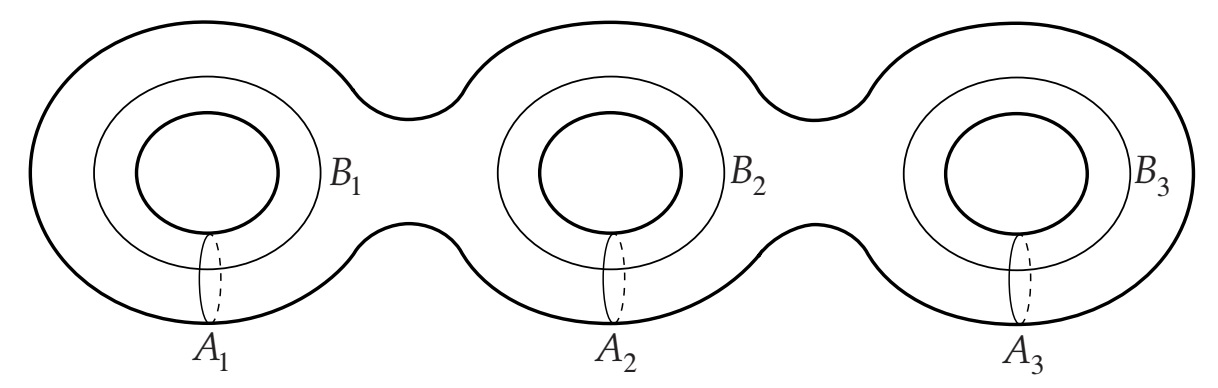
\includegraphics[width=0.8\textwidth]{figure/Fig9.1.jpg}\\
		\caption{A genus 3 surface, with $A$-cycles and $B$-cycles marked.}\label{Fig9.1}
	\end{center}
\end{figure}


The $A$-cycles and $B$-cycles are complete, in that every closed path is homotopic to a series of $A$-cycles or $B$-cycles.
In fact, they are overcomplete: the path
\begin{equation}
	(A_{1} B_{1}^{-1} A_{1}^{-1} B_{1})(A_{2} B_{2}^{-1} A_{2}^{-1} B_{2}) \ldots(A_{g} B_{g}^{-1} A_{g}^{-1} B_{g}) \label{9.2.4}
\end{equation}
can be contracted to a point, and the corresponding product must be the identity.
Counting moduli, there are 6 real parameters in each $PSL(2, \mathds{R})$ element, giving $6g$, subtracting 3 from the constraint \eqref{9.2.4}, 
and since the total $PSL(2, \mathds{R})$ gives an equivalent surface, subtract another 3, totaling $6g-6$.

Although the Schottky parametrization is similar to the Fuchsian parametrization, they have quite different properties. In particular, the complex structure of the latter is less obvious, and correspondingly, the extension to superstrings is not as simple.
\subsection*{Period Matrix}
The moduli parameter $\tau$ of the torus can be naturally generalized to a $g \times g$ matrix at genus $g$. To see this, we first need Abelian differentials or holomorphic 1-forms. 
They are world-sheet fields $\omega_{a}$ with the following properties in complex coordinates:
\begin{equation}
	\partial_{\bar{z}} \omega_{z} = 0 \:, \quad \omega_{\bar{z}} = 0 \:.
	\label{9.2.5}
\end{equation}
There are exactly $g$ such fields, and $g$ further satisfies conjugation relations. This originates from the Riemann-Roch theorem \eqref{5.3.22}. The Abelian differentials \eqref{9.2.5} and their conjugates are exactly the kernel of the operator $P_{0}^{T}$, 
for which the Riemann-Roch theorem is:
\begin{equation}
	\operatorname{dim} \operatorname{ker} P_{0}^{T}-\operatorname{dim} \operatorname{ker} P_{0}=-\chi=2 g-2 \:.
	\label{9.2.6}
\end{equation}
The operator $P_{0}$ acts on the scalar fields $c$ and $\tilde{c}$ with $h=0$, thus reducing to the ordinary gradient. There are always 2 zero modes ($c=$ constant or $\tilde{c}=$ constant), 
hence $\operatorname{dim}\operatorname{ker}P_{0}^{T}=2g$.
\begin{tcolorbox}[breakable]
	\begin{remark}
		Conventions. As in Chapter \ref{cha:5}, $P_n$ maps tensors with $n$ lower $z$ indices (and their conjugates) to $n+1$ indices, $P_n\colon t_{z\cdots z}\mapsto\nabla_{\bar z}t_{z\cdots z}$ up to normalization. Dimensions count independent solutions in the holomorphic and antiholomorphic sectors together. With this counting the Riemann--Roch theorem reads
		\begin{equation*}
			\dim\ker P_n-\dim\ker P_n^T=(2n+1)\chi ,
		\end{equation*}
		and for $n=1$ it is the familiar statement $\#\text{CKVs}-\#\text{moduli}=3\chi$. For $n=0$ the fields are the weight-zero ghosts $c,\tilde c$ of the text:
		\begin{align*}
			\ker P_0&=\{\partial_{\bar z}c=0,\ \partial_z\tilde c=0\}\eqs{1}\{c=\text{const},\ \tilde c=\text{const}\},\qquad\dim\ker P_0=2,\\
			\ker P_0^T&=\{\partial_{\bar z}\omega_z=0,\ \partial_z\omega_{\bar z}=0\},\qquad
			\dim\ker P_0^T\eqs{2}2-\chi=2g .
		\end{align*}
		At (1) a holomorphic function on a compact surface is constant. At (2) Riemann--Roch with $n=0$ was used. The kernel of $P_0^T$ consists of the holomorphic 1-forms $\omega_z\,\dif z$ and their complex conjugates, so there are exactly $g$ Abelian differentials. The same number follows from Hodge theory: the space of real harmonic 1-forms has dimension $b_1=2g$, and every harmonic form splits uniquely as $\omega+\bar\omega$ with $\omega$ holomorphic.
	\end{remark}
\end{tcolorbox}

Line integrals of 1-forms are coordinate invariants.
Then the natural basis for Abelian differentials is $\omega_{z i}, i=1, \ldots, g$, defined as:
\begin{equation}
	\oint_{A_{i}} \dif z \: \omega_{z j}=\delta_{i j} \:.
	\label{9.2.7}
\end{equation}
Then the period matrix:
\begin{equation}
	\tau_{i j}=\oint_{B_{i}} \dif z\: \omega_{z j} \label{9.2.8}
\end{equation}
characterizes the complex structure of the surface. When the genus is 1, $\omega_{z}$ is a constant, which is the usual $\tau$.

It can be proven that $\tau_{ij}$ is symmetric, so it has $\frac{1}{2} g(g+1)$ complex parameters.
When $g=1,2,3$ it equals the number of complex moduli. 
When $g \geq 4$, it will be larger, so not all period matrices correspond to Riemann surfaces.
The $\theta$-function \eqref{7.2.36} has a natural genus-$g$ generalization, 
where $\tau$ becomes the period matrix, and $\nu, n, a, b$ become $g$-component vectors.
\begin{tcolorbox}[breakable]
	\begin{proof}[Symmetry and positivity of $\tau_{ij}$]
		Cut $M$ along the cycles $A_k,B_k$ to obtain a simply connected $4g$-gon $F$ with boundary $\prod_kA_kB_kA_k^{-1}B_k^{-1}$, with the orientation for which the intersection number is $A_k\cdot B_l=\delta_{kl}$. For closed 1-forms $\alpha,\beta$, write $\alpha=\dif f$ on $F$. The values of $f$ on the two copies of an edge differ by a period of $\alpha$, which gives the Riemann bilinear relation
		\begin{equation*}
			\int_M\alpha\wedge\beta=\oint_{\partial F}f\beta=\sum_{k=1}^g\Bigl(\oint_{A_k}\alpha\oint_{B_k}\beta-\oint_{B_k}\alpha\oint_{A_k}\beta\Bigr).
		\end{equation*}
		With $\alpha=\omega_i=\omega_{zi}\dif z$ and $\beta=\omega_j$, the left side vanishes because $\dif z\wedge\dif z=0$:
		\begin{equation*}
			0\eqs{1}\sum_k\bigl(\delta_{ki}\tau_{kj}-\tau_{ki}\delta_{kj}\bigr)=\tau_{ij}-\tau_{ji} .
		\end{equation*}
		At (1) the normalization \eqref{9.2.7} and the definition \eqref{9.2.8} were used. So $\tau$ is symmetric. For positivity, take $\omega=\sum_ic_i\omega_i=f(z)\dif z$ with $c\in\mathbb C^g$ nonzero, and $\beta=\bar\omega$, whose periods are complex conjugated:
		\begin{align*}
			\int_M\omega\wedge\bar\omega&\eqs{2}\sum_k\bigl(c_k(\bar\tau\bar c)_k-(\tau c)_k\bar c_k\bigr)\eqs{3}-2\mi\,c^T(\operatorname{Im}\tau)\bar c ,\\
			\int_M\omega\wedge\bar\omega&=\int_M|f|^2\,\dif z\wedge\dif\bar z=-2\mi\int_M|f|^2\,\dif x\wedge\dif y .
		\end{align*}
		At (2) $\oint_{A_k}\omega=c_k$ and $\oint_{B_k}\omega=(\tau c)_k$. At (3) the symmetry of $\tau$ was used. Comparing the two lines, $c^T(\operatorname{Im}\tau)\bar c=\int|f|^2\,\dif x\,\dif y>0$, so $\operatorname{Im}\tau$ is positive definite. This is exactly what makes the genus-$g$ theta function $\sum_{n\in\mathbb Z^g}\exp(\pi\mi\,n\cdot\tau\cdot n+2\pi\mi\,n\cdot\nu)$ converge.

		Counting: a symmetric complex $g\times g$ matrix has $\frac12g(g+1)$ entries, compared with $3g-3$ complex moduli for $g\ge2$ (and 1 for $g=1$):
		\begin{equation*}
			g=1:\ 1=1,\qquad g=2:\ 3=3,\qquad g=3:\ 6=6,\qquad g=4:\ 10>9,
		\end{equation*}
		and for $g\ge4$ the difference $\frac12(g-2)(g-3)$ is positive. That is why only a subvariety of period matrices comes from Riemann surfaces.
	\end{proof}
\end{tcolorbox}

\subsection*{Hyperelliptic Surfaces}

There is another description that is sometimes very useful.
Consider the space $S_{2} \times S_{2}$ with coordinates $z$ and $y$. Consider the submanifold given by the following equation:
\begin{equation}
	y^{2}=\prod_{i=1}^{2 k}(z-Z_{i}) \:, \label{9.2.9}
\end{equation}
where $Z_{i}$ are complex parameters. Projected onto the $z$-coordinate, there are two surfaces connected by $k$ branch cuts.
This gives a surface with $g=k-1$ handles. When projected to $z$, the branch points are singular, 
but the entire surface \eqref{9.2.9} is not singular: $y$ is a good local coordinate.

This surface depends on $2k$ complex $Z_{i}$, but some are redundant under Möbius transformations, leaving $2k-3=2g-1$ complex parameters. When $g=1,2$, this is the same as the number of moduli;
but when $g \geq 3$, the number of moduli is larger, and only special surfaces take the form of \eqref{9.2.9}, which are called hyperelliptic surfaces.
\begin{tcolorbox}[breakable]
	\begin{remark}
		\emph{Genus.} The projection $(z,y)\mapsto z$ is a double cover of the sphere. It is branched at the $2k$ roots $Z_i$ and not at $z=\infty$, because the degree $2k$ is even: $y\approx\pm z^k$ gives two distinct points there. The Riemann--Hurwitz formula, $\chi(M)=2\chi(S_2)-\sum_{\text{branch points}}(e-1)$ with ramification index $e=2$, gives
		\begin{equation*}
			2-2g\eqs{1}2\cdot2-2k\cdot1=4-2k\quad\Longrightarrow\quad g=k-1 .
		\end{equation*}
		At (1) each branch point was counted with $e-1=1$. Near $Z_1$, $y^2\approx C(z-Z_1)$ with $C=\prod_{i\ne1}(Z_1-Z_i)\ne0$, so $z-Z_1\approx y^2/C$. Thus $y$ is a good coordinate at the branch point, while $z$ is two-to-one there.

		\emph{Parameters.} The $2k$ branch points modulo the 3 complex M\"obius parameters leave $2k-3=2(g+1)-3=2g-1$. Compared with $3g-3$ (or 1 at $g=1$): $g=1$ gives $1=1$, $g=2$ gives $3=3$, and $g=3$ gives $5<6$. The deficit $(3g-3)-(2g-1)=g-2$ grows with $g$.
	\end{remark}
\end{tcolorbox}

\section{Sewing and cutting world-sheets}  \label{sec:9.3}

A useful concept in analyzing string amplitudes is the relationship between higher genus amplitudes and lower genus amplitudes. The key element is the plumbing fixture. 
This is used to construct higher genus surfaces from lower genus ones.
Consider two world-sheets $M_{1}, M_{2}$ with coordinates $z_{1}, z_{2}$. 
We can connect them to form a new world-sheet $M$ as follows: Let $q$ be a complex parameter. Subtract a disk $|z_{1}|<(1-\epsilon)|q|^{1/2}$ from $M_{1}$, 
and subtract $|z_{2}|<(1-\epsilon)|q|^{1/2}$ from $M_{2}$, where $\epsilon$ is a small quantity.
To form a surface, identify points such that:
\begin{equation}
	z_{1} z_{2}=q \:. \label{9.3.1}
\end{equation}
As shown in Figure \ref{Fig9.2}. The disk regions:
\begin{equation}
	(1-\epsilon)^{-1}|q|^{1/2} > |z_{1}| > (1-\epsilon)|q|^{1/2} \label{9.3.2}
\end{equation}
are sewn together as shown in the figure. A representation of this construction is:
\begin{equation}
	M=M_{1} \infty M_{2}(z_{1}, z_{2}, q) \:. \label{9.3.3}
\end{equation}
This notation emphasizes that the corresponding surface depends on the choice of local coordinates.
If different local coordinates $z_{1}^{\prime}$ and $z_{2}^{\prime}$ are chosen, different circles will be cut out, and the connecting surfaces will generally be different. 
These two coordinate charts might also be located in different parts of a single surface $M_{0}$. Then the plumbing fixture construction adds a handle to the surface. This is denoted as:
\begin{equation}
	M=M_{0} 8(z_{1}, z_{2}, q)  \:. \label{9.3.4}
\end{equation}
The symbols `$\infty$' and `8' are used to distinguish the two sewing processes. The parameter $q$ is not strictly necessary—taking $z_{1}^{\prime}=z_{1} q^{-1/2}$, $z_{2}^{\prime}=z_{2} q^{-1/2}$, 
and $q^{\prime}=1$ gives an equivalent surface.
Introducing $q$ is to facilitate the discussion of the behavior as $q$ varies when the coordinate charts are fixed.

\begin{figure}[!htbp]
	\begin{center}
		%width=0.8\textwidth,bb=0 0 877 729
		%1px=0.75pt
		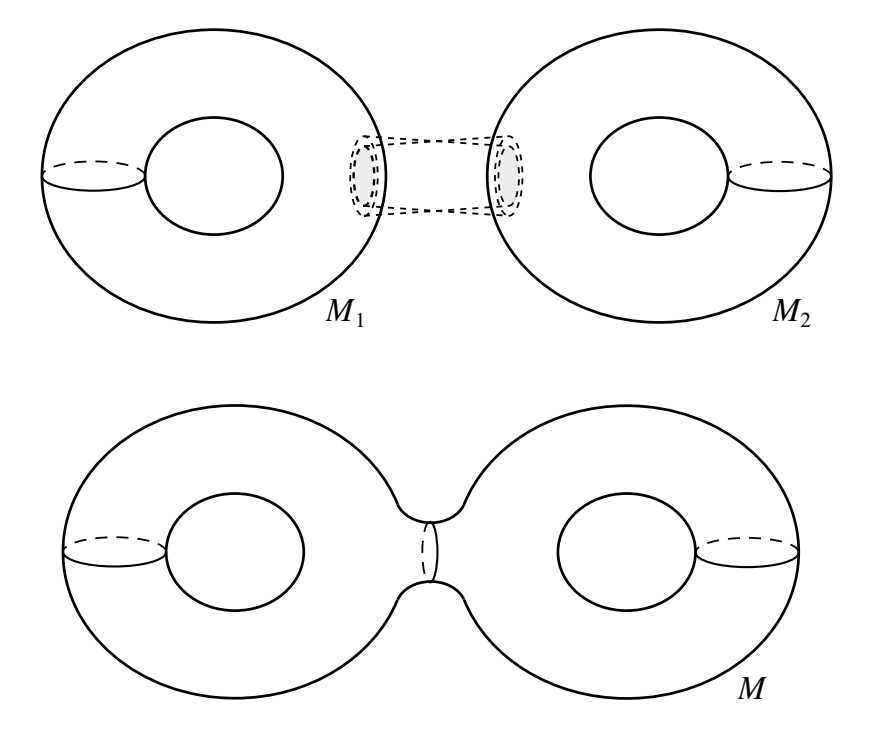
\includegraphics[width=0.8\textwidth]{figure/Fig9.2.jpg}\\
		\caption{Removing a disk from each of two world-sheets and then gluing the edges of the disks together.}\label{Fig9.2}
	\end{center}
\end{figure}

We can also reverse this construction. Given any Riemann surface $M$ and a non-intersecting curve $C$ on it, one can always find holomorphic coordinates $z_{1}=z_{2}^{-1}$ in a neighborhood of $C$ 
such that $C$ is given by $|z_{1}| = |z_{2}| = |q|^{1/2}$.
Cutting $C$ (undoing the equivalence relation $z_{1} z_{2}=q$) and gluing back disks $|z_{1}|<|q|^{1/2}$ and $|z_{2}|<|q|^{1/2}$ produces $M_{1}$ and $M_{2}$ (or $M_{0}$), 
such that $M$ can be regenerated through the sewing operation—depending on whether cutting $C$ makes the surface disconnected, we use sewing \eqref{9.3.3} or \eqref{9.3.4}, respectively.


\begin{figure}[!htbp]
	\begin{center}
		%width=0.8\textwidth,bb=0 0 994 578
		%1px=0.75pt
		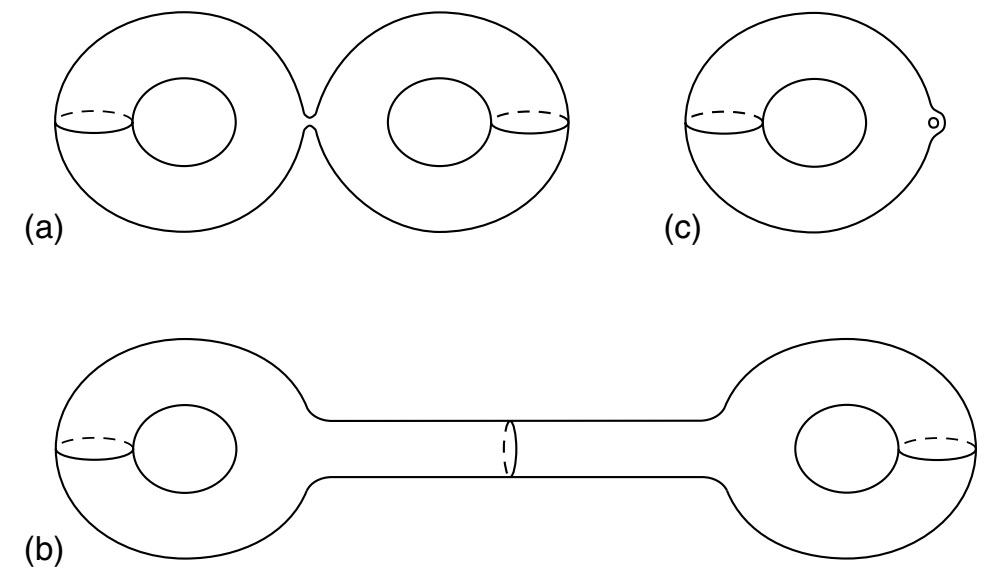
\includegraphics[width=0.8\textwidth]{figure/Fig9.3.jpg}\\
		\caption{Three representations of a genus 2 surface with degenerate circles.}\label{Fig9.3}
	\end{center}
\end{figure}

For the genus 2 example in Figure \ref{Fig9.2}, consider the case where $q \ll 1$.
Figure \ref{Fig9.3}a shows $M$ in this situation. 
In the overlapping region, we smoothly insert a metric between $\dif z_{1} \dif \bar{z}_{1}$ and $\dif z_{2} \dif \bar{z}_{2}$. 
The surface is pinched into a circle with a radius of order $|q|^{1/2} $. Through a Weyl transformation, one can always find a metric such that the radius remains of order 1, as shown in Figure \ref{Fig9.3}b.
Since the action of a Weyl transformation is isometric, its effect is that the handle's length becomes very large, of order $-\ln |q|$. The handle regions $|z_{1}|<1, |z_{2}|<1$ are equivalent to a cylinder:
\begin{equation}
	\ln |q|<\operatorname{Im} w<0 \:, \quad w \cong w+2 \pi \:.
	\label{9.3.5}
\end{equation}
where $z_{1}=\exp (-\mi w)$ and $z_{2}=q \exp (\mi w) $.
\begin{tcolorbox}[breakable]
	\begin{remark}
		The two coordinates are compatible with the sewing, since $z_1z_2=\me^{-\mi w}q\me^{\mi w}=q$. Writing $w=u+\mi v$,
		\begin{equation*}
			|z_1|=\me^{v}<1\iff v<0,\qquad |z_2|=|q|\me^{-v}<1\iff v>\ln|q| ,
		\end{equation*}
		and $w\cong w+2\pi$ because $z_1,z_2$ are single valued. The overlap of the two unit disks is therefore the cylinder \eqref{9.3.5}, with circumference $2\pi$ and length $-\ln|q|$. In the flat metric $\dif w\,\dif\bar w=\dif z_1\dif\bar z_1/|z_1|^2$, which is Weyl equivalent to $\dif z_1\dif\bar z_1$, the handle becomes a long tube as $q\to0$.
	\end{remark}
\end{tcolorbox}
\noindent Figure \ref{Fig9.3}c gives another representation of the same surface.
The disk regions $O(|q|)<|z|<O(1)$ around the small handles are conformally equivalent to the long cylinder in Figure \ref{Fig9.3}b. 
In the form of Figure \ref{Fig9.3}a, this picture can be considered as a Weyl transformation where all $M_{2}$ have been reduced.
In all these pictures, it is clear that the surface becomes special in the limit $q \rightarrow 0$. This handle is called a pinch or degenerate. This is an example of a boundary of moduli space. 
Moduli space boundaries are very important because every divergence must originate here. In fact, we will see that every boundary is in this form, where one or more handles are pinched. 
For a genus-2 surface, there is another way a single handle can degenerate if the $A$-cycle or $B$-cycle pinches.
This corresponds respectively to starting from a single torus and constructing a genus-2 torus via the `8' operation (rather than from two tori via the `$\infty$' operation) and taking $q \rightarrow 0$.

By repeatedly using the cutting operation, we will find an interesting fact: every Riemann surface will degenerate into spheres with 3 punctures. A puncture is a marked point with a specific complex coordinate near it; 
this is the data required for plumbing fixture sewing. In other words, every Riemann surface can be constructed from spheres with 3 punctures via sewing. For example, Figure \ref{Fig9.4} gives three ways to construct a genus 2 surface with 4 vertex operators. 
For each sewing operation, there is a complex modulus $q$. For each construction in Figure \ref{Fig9.4}, this gives 7 single complex moduli.
These correspond to the $3g-3=3$ complex moduli of a genus 2 surface plus the 4 positions of the vertex operators.

\begin{figure}[!htbp]
	\begin{center}
		%width=0.8\textwidth,bb=0 0 954 553
		%1px=0.75pt
		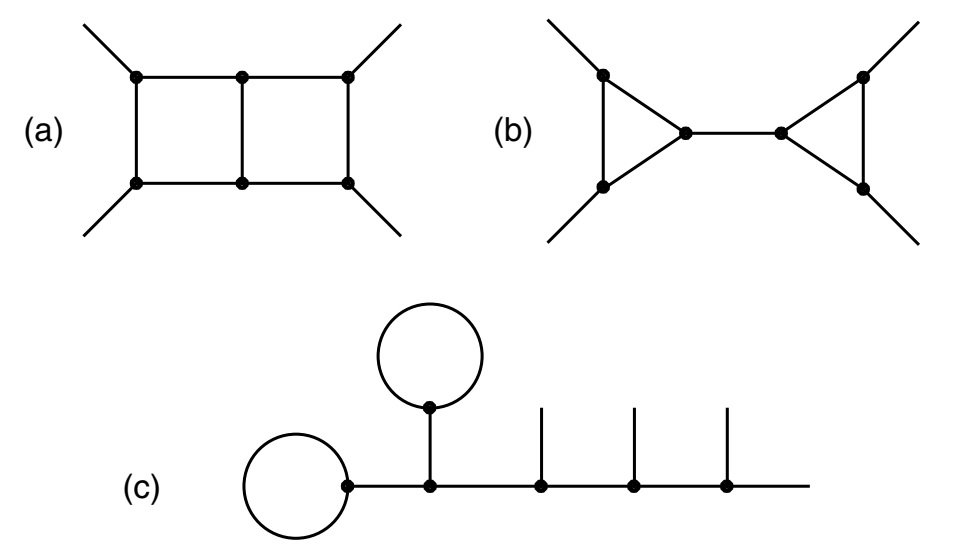
\includegraphics[width=0.8\textwidth]{figure/Fig9.4.jpg}
		\caption{Some sewing constructions for genus 2 surfaces with 4 operators. Each vertex is a sphere with three holes, each internal line represents a plumbing fixture construction, and each external line represents a vertex operator.}\label{Fig9.4}
	\end{center}
\end{figure}

\subsection*{Graph-theoretic decomposition}

Figure \ref{Fig9.4} is reminiscent of Feynman diagrams. We now describe a Feynman-like diagrammatic decomposition of the moduli space. The vertices are much more complicated than in \ref{Fig9.4}, potentially with any number of external lines and internal corrections in string loops. 
The key to this construction lies in making the properties of the moduli space boundary obvious.

The statement is: the integral over the moduli space is given by a sum over Feynman diagrams.
The internal propagator lines in the diagram represent the sewing operation, with the sewing parameter $q$ to be integrated out being in some standard region, such as $|q|<1$.  
The $n$-point vertices represent Riemann surfaces with $n$ punctures. We will see that surfaces in the vertices are to be integrated over some internal part of the moduli space and summed over genus. 
The sewing operation refers to specifying complex coordinates for each point to be sewn, so the vertex definition must include the choice made at each point. The set of surfaces of genus $g$ appearing in the $n$-point vertex is denoted as $\mathscr{V}_{g,n}$. 
External lines represent vertex operators.
\begin{figure}[!htbp]
	\begin{center}
		%width=0.8\textwidth,bb=0 0 343 313
		%1px=0.75pt
		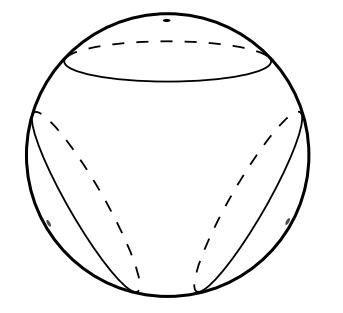
\includegraphics[width=0.8\textwidth]{figure/Fig9.5.jpg}\\
		\caption{A trilinear vertex, a sphere with three marked points and three sewing circles.}\label{Fig9.5}
	\end{center}
\end{figure}

We illustrate this construction with an example. Starting from the three-point vertex $\mathscr{V}_{0,3}$, as shown in Figure \ref{Fig9.5}, it is a sphere with 3 marked points and 3 sewing circles. 
In the complex coordinates near the corresponding points, the sewing circles are unit circles. Steps to build a sphere with four points: take two such vertices, remove the interior of one sewing circle from each, and then glue them at both ends of a cylinder; 
this is equivalent to the plumbing fixture construction. This corresponds to the Feynman diagram in Figure \ref{Fig9.6}a; the cylinder length is $-\ln |q|$ (with circumference adjusted to $2\pi$).
Integrating over $|q|<1$ 
and summing over the other two channels only gives a part of the integration region of the sphere with four points, as shown in Figure \ref{Fig9.6}b. The shaded region is covered, but the non-shaded region is missing.

\begin{figure}[!htbp]
	\begin{center}
		%width=0.8\textwidth,bb=0 0 987 482
		%1px=0.75pt
		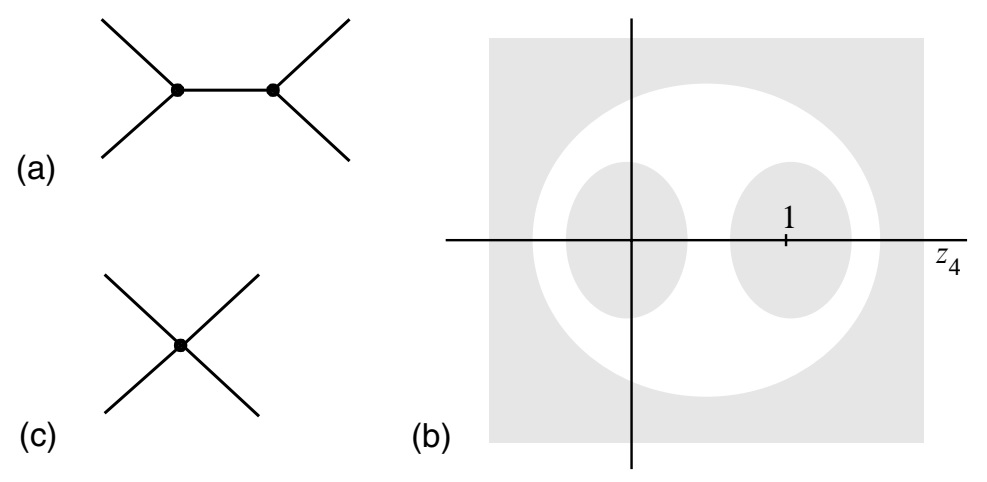
\includegraphics[width=0.8\textwidth]{figure/Fig9.6.jpg}\\
		\caption{(a) Constructing a sphere with four vertex operators. (b) The region covered by this diagram in the $z$-plane. (c) Additional vertex required to give the correct amplitude. Integration for a four-hole sphere in the non-shaded region.}\label{Fig9.6}
	\end{center}
\end{figure}

Let us provide further explanation.
For trilinear vertices, place the points at $0,1, \infty$ on the sphere, and choose coordinate systems $z^{(0)}, z^{(1)}$, $z^{(\infty)}$, 
so the three sewing circles are $|z^{(0,1, \infty)}|=1$. This choice should be invariant under the 6 Möbius transformations that permute the vertices, making the vertex symmetric.
There are multiple possible choices, for example:
\begin{equation}
	z^{(0)}=\frac{a z}{z-2}, \quad z^{(1)}=\frac{a(z-1)}{z+1}, \quad z^{(\infty)}=\frac{a}{2 z-1} \:, \label{9.3.6}
\end{equation}
where $a$ is an arbitrary constant. When $a \geq 3$, the sewing circles do not overlap, ensuring that the plumbing fixture construction gives a good surface for all $q \leq 1$.
Readers can prove that sewing the $z^{(\infty)}$ and $z^{(0)}$ coordinate charts from two spheres under parameter $q$ produces a sphere with vertex operators at $0,1, \frac{1}{2}(1+a^{2}/q)$ and $\frac{1}{2}(1-a^{2}/q)$. 
Under Möbius transformation, this is equivalent to vertex operators at $0,1, \infty$, and:
\begin{equation}
	z_{4}=(q-a^{2})^{2}/4 a^{2} q \:.
	\label{9.3.7}
\end{equation}
\begin{tcolorbox}[breakable]
	\begin{remark}
		\emph{The sewing circles.} The disk $|z^{(0)}|<1$ is $|z|<|z-2|/a$, an Apollonius disk for the points $0,2$ with ratio $1/a$. Its center is $-2/(a^2-1)$ and its radius $2a/(a^2-1)$, so on the real axis it spans $[-2/(a-1),\,2/(a+1)]$. The map $z\to1-z$ sends $z^{(0)}\to z^{(1)}$, so the disk around $1$ spans $[(a-1)/(a+1),\,(a+1)/(a-1)]$. The disk around $\infty$ is $|z^{(\infty)}|<1$, i.e.\ $|z-\frac12|>\frac a2$. Hence
		\begin{align*}
			\text{disks at }0,1\text{ disjoint}&\iff\frac{2}{a+1}\le\frac{a-1}{a+1}\iff a\ge3,\\
			\text{disk at }0\text{ inside }|z-\tfrac12|\le\tfrac a2&\iff\frac12+\frac{2}{a-1}\le\frac a2\iff(a-1)^2\ge4\iff a\ge3 .
		\end{align*}
		At $a=3$ the three circles touch pairwise, at $z=\frac12$ and $z=-1,2$. For $a>3$ they are disjoint, so the plumbing fixture is well defined for all $|q|\le1$.

		\emph{The sewn sphere.} Sew sphere $A$ with its $z^{(\infty)}$ chart to sphere $B$ (coordinate $z'$) with its $z'^{(0)}$ chart, $z^{(\infty)}z'^{(0)}=q$. The map is M\"obius, so it extends to a global identification of $B$ with $A$:
		\begin{equation*}
			\frac{a}{2z-1}=\frac{q(z'-2)}{az'}\quad\Longrightarrow\quad z=\frac12\Bigl(1+\frac{a^2}{q}\frac{z'}{z'-2}\Bigr).
		\end{equation*}
		The surviving operators of $B$ are at $z'=1$ and $z'=\infty$, where $z'/(z'-2)=-1$ and $1$. They land at $z_\mp=\frac12(1\mp a^2/q)$, while the operators of $A$ stay at $0$ and $1$. This proves the statement in the text. Now send $z_+\to\infty$ with the M\"obius map $f(z)=z(1-z_+)/(z-z_+)$, which fixes $0$ and $1$:
		\begin{equation*}
			z_4=f(z_-)=\frac{z_-(1-z_+)}{z_--z_+}\eqs{1}\frac{\frac{q-a^2}{2q}\cdot\frac{q-a^2}{2q}}{-a^2/q}=-\frac{(q-a^2)^2}{4a^2q} .
		\end{equation*}
		At (1) $z_-=1-z_+=(q-a^2)/2q$ and $z_--z_+=-a^2/q$. The other assignment, $z_-\to\infty$, gives $(q+a^2)^2/4a^2q=1-f(z_-)$ instead. All six cross-ratio values follow from $\lambda=f(z_-)$ by $\lambda\to1-\lambda$ and $\lambda\to1/\lambda$. For generic $q$ none of them equals the expression printed in \eqref{9.3.7}, which is $-f(z_-)$. With the charts \eqref{9.3.6} and $z_1z_2=q$, the correct value is therefore $z_4=-(q-a^2)^2/4a^2q$ or one of its cross-ratio images; the printed sign appears to be a typo. The statement that matters is unaffected: $|z_4|\approx a^2/4|q|\to\infty$ as $q\to0$, and $|q|\le1$ maps to a neighborhood of $z_4=\infty$ (for $|q|=1$, $|z_4|\ge(a^2-1)^2/4a^2$). This neighborhood is the outer shaded region of Figure \ref{Fig9.6}b.
	\end{remark}
\end{tcolorbox}
As $q$ runs over the unit disk, $z_{4}$ covers the outer shaded region of Figure \ref{Fig9.6}b. Permuting the vertices gives the other two regions. 
We could try to take smaller $a$, so that the shaded regions grow, but they will eventually overlap and double-count some surfaces, while other surfaces still will not be produced. 
They will never exactly cover the entire plane, so we also need to add an explicit four-point vertex $\mathscr{V}_{0,4}$, given by a sphere with 4 marked points, 
and integrate over the non-shaded region of the $z$-plane.
Since there is still a choice for each hole's coordinate for each value of $z_{4}$, this does not completely define $\mathscr{V}_{0,4}$. 
Connect the boundaries of the shaded and non-shaded regions in a smooth way. Note that the Feynman diagram in Figure \ref{Fig9.6}a contains all asymptotic regions $z_{4} \rightarrow 0,1, \infty$, 
while the four-point vertex only contains non-degenerate surfaces. Then the behavior in this limit is clearly given by the limit $q \rightarrow 0$: this is why plumbing fixture construction is useful.

As an example, sewing two circles of a single vertex at both ends of a cylinder gives a torus with one vertex operator.
This covers the $\operatorname{Im} \tau \rightarrow \infty$ limit of the torus moduli space, but the internal region is lost and must be added back through a manual vertex region $\mathscr{V}_{1,1}$.

This construction can be extended inductively. Each sewing operation always adds:
\begin{equation}
	r = 3g + n - 2  \label{9.3.8}
\end{equation}
parameters.
The original sphere with three holes, vertex $\mathscr{V}_{0,3}$, has $r=1$. The `8' operation gives $r=r_{0}+1$, while the `$\infty$' operation gives $r=r_{1}+r_{2}$. 
Thus, $\mathscr{V}_{0,4}$ and $\mathscr{V}_{1,1}$ both have $r=2$. It has been proven that $\mathscr{V}_{g, n}$ can be constructed by induction on $r$, 
thus covering the entire moduli space as claimed earlier.
\begin{tcolorbox}[breakable]
	\begin{remark}
		Note $r=(3g-3+n)+1=\dim_{\mathbb C}\mathscr M_{g,n}+1$, one more than the number of complex moduli of a genus-$g$ surface with $n$ punctures. The rules quoted follow directly:
		\begin{align*}
			\mathscr V_{0,3}:&\quad r=0+3-2=1,\\
			\text{`8'}:\ (g,n)\to(g+1,n-2):&\quad r'=3(g+1)+(n-2)-2=r+1,\\
			\text{`}\infty\text{'}:\ (g_1,n_1),(g_2,n_2)\to(g_1+g_2,n_1+n_2-2):&\quad r'=3(g_1+g_2)+n_1+n_2-4=r_1+r_2 .
		\end{align*}
		Each sewing introduces one complex parameter $q$, which matches the moduli count. Under `8', $3g-3+n$ increases by $3-2=1$. Under `$\infty$', $\dim\mathscr M_{g_1+g_2,n_1+n_2-2}=\dim\mathscr M_{g_1,n_1}+\dim\mathscr M_{g_2,n_2}+1$. For example, $\mathscr V_{0,4}$ and $\mathscr V_{1,1}$ both have $r=2$, one modulus. For Figure \ref{Fig9.4}, a graph with only cubic vertices, $V$ vertices, $E$ internal lines and $n$ external lines satisfies $3V=2E+n$ and $E-V+1=g$. Hence $E=3g-3+n$: for $g=2$, $n=4$ this gives $7$ plumbing parameters, the $3+4$ complex moduli quoted in the text.
	\end{remark}
\end{tcolorbox}
A clearer construction is given below. On any Riemann surface, there exists a unique minimum-area metric, defined as the metric with minimum area subject to the constraint that every non-trivial closed curve has a length of at least $2\pi$. 
Each point on this surface lies on at least one saturating geodesic, a non-trivial closed curve with length exactly $2\pi$. 
Saturating geodesics that can be continuously transformed into other saturating geodesics do not intersect themselves, and each set of homotopic saturating geodesics forms an annulus (topologically a torus) on the surface. 
Different annuli cover the entire surface but may overlap. The height $h$ of such an annulus is defined as the shortest distance between its two boundary geodesics. The idea of a minimum-area metric can be extended to surfaces with holes 
by treating circles around the holes as non-trivial.
The minimum-area metric near a hole is of the form $\dif z \dif \bar{z} / z \bar{z}$, a semi-infinite cylinder of radius $2\pi$. 
Thus there are two types of annuli: one internal and finite, the other gathering at holes and semi-infinite, terminating inside the surface.

We can now use this construction to describe $\mathscr{V}_{g, n}$.
Take all Riemann surfaces with $n$ holes, imposing the constraint that any internal annulus has a height less than $2\pi$ under the minimum-area metric. 
Cut the semi-infinite cylinders, leaving a stub of length $\pi$, and glue them into usual disks, inserting vertex operators at the bottom of the stubs. With these vertices, the sum of Feynman diagrams will exactly cover the moduli space once. 
It can be proven that sewing minimum-area surfaces still produces minimum-area surfaces.
Annuli with height less than $2\pi$ are clearly contained in the vertices, while annuli with height greater than $2\pi$ will be produced by the sewing operators on the stubs, 
with the corresponding height being $2\pi$ from the stubs plus $-\ln |q|$ from the plumbing fixture; as $q$ is integrated, this runs from $2\pi$ to $\infty$. The minimum length constraint and maximum height ensure that degenerate surfaces do not appear in the vertices, 
so they only appear when one or more $q$ tend to zero, which is exactly what was to be proven.
\section{Sewing and cutting CFTs} \label{sec:9.4}



\begin{figure}[!htbp]
	\begin{center}
		%width=0.8\textwidth,bb=0 0 957 668
		%1px=0.75pt
		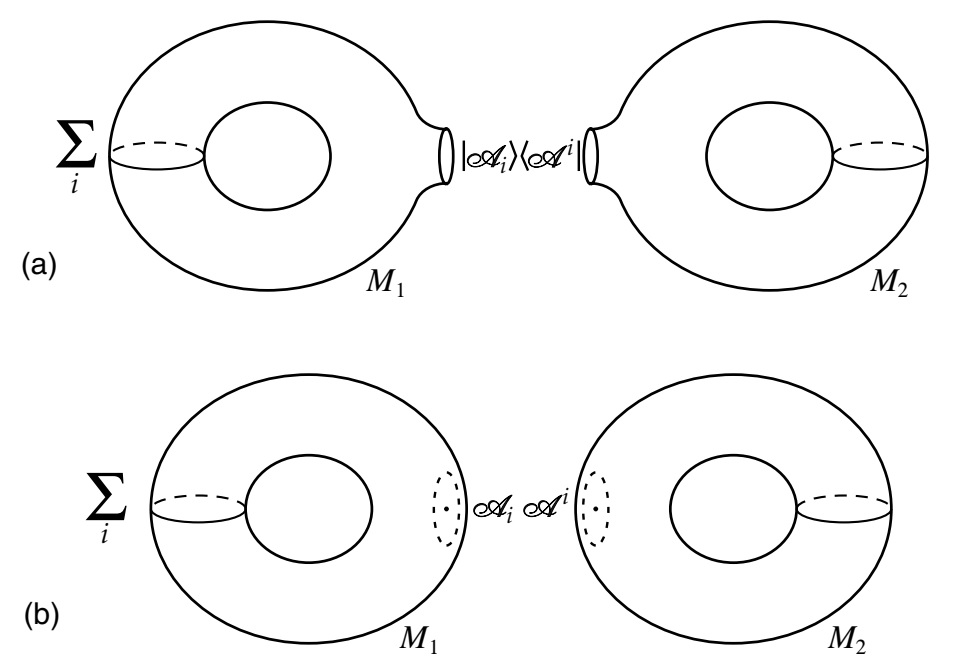
\includegraphics[width=0.8\textwidth]{figure/Fig9.7.jpg}\\
		\caption{(a) Cutting the path integral on $M$ by inserting a complete set of boundary states. (b) Each state is replaced by a disk with a local operator.}\label{Fig9.7}
	\end{center}
\end{figure}

By sewing lower genus Riemann surfaces together, we described higher genus Riemann surfaces. Using the sewing properties of the path integral, similarly, CFTs on higher genus surfaces can be associated with lower-order amplitudes. This relationship is shown in Figure \ref{Fig9.7}.
For clarity, we first discuss the case $q=1$. The path integral on $M$ is cut along the circle $|z_{1}|=|z_{2}|=1$, inserting a complete set of boundary states. Then each boundary state is replaced by a disk with a corresponding local operator, 
leaving the uncut world-sheets $M_{1}$ and $M_{2}$.
The precise form of this result is:
\begin{equation}
	\langle {}_{\cdots 1} {}_{\cdots 2}\rangle_{M} = \sum_{i j}\Bigl \langle {}_{\cdots 1} \mathscr{A}_{i}^{(z_{1})}\Bigr\rangle_{M_{1}} 
	\mathsf{G}^{ij} \Bigl\langle\mathscr{A}_{j}^{(z_{2})} {}_{\cdots 2}\Bigr\rangle_{M_{2}} \:.
	\label{9.4.1}
\end{equation}
We allow arbitrary additional insertions ${}_{\cdots 1}$ and ${}_{\cdots 2}$ on $M_{1}$ and $M_{2}$; they must be located outside the circles $|z_{1}|=1$ and $|z_{2}|=1$. 
We have not yet specified any particular orthogonality for this basis; an appropriate invertible matrix $\mathsf{G}^{i j}$ still needs to be decided.
Instead of the handles, the insertions $\mathscr{A}_{i}$ and $\mathscr{A}_{j}$ 
are implicitly located at the origins of the $z_{1}$ and $z_{2}$ coordinate systems, respectively.

Now consider the case where $M_{2}$ is a sphere, let the sewing coordinate $z_{2}$ be denoted as $u$, and let ${}_{\cdots 2}$ be a local operator $\mathscr{A}_{k}$ at $z=0$.
From the plumbing fixture construction, we have $z_{1} u=1$, and from the sphere, we have $z u=1$, so we can extend $z_{1}=z$ to the entire sewing region. 
The sewn surface $M$ is the same as $M_{1}$ with an extra operator $\mathscr{A}_{k}$ at $z_{1}=0$.
Then \eqref{9.4.1} becomes:
\begin{equation}
	\Bigl \langle {}_{\cdots 1} \mathscr{A}_{k}^{(z_{1})}\Bigr\rangle_{M_{1}} = 
	\sum_{i j}\Bigl\langle {}_{\cdots 1} \mathscr{A}_{i}^{(z_{1})}\Bigr\rangle_{M_{1}} \mathsf{G}^{ij} 
	\Bigl\langle\mathscr{A}_{j}^{(u)} \mathscr{A}_{k}^{(z)}\Bigr\rangle_{S_{2}} \:.
	\label{9.4.2}
\end{equation}
The two-point function $\langle\mathscr{A}_{j}^{(u)} \mathscr{A}_{k}^{(z)}\rangle_{S_{2}}$ is exactly the inner product $\lAngle j \vert k\rangle=\mathsf{G}_{jk}$. 
Then \eqref{9.4.2} implies:
\begin{equation}
	\mathsf{G}^{ij} \mathscr{G}_{jk} = \delta_{k}^{i} \label{9.4.3}
\end{equation}
or:
\begin{equation}
	\mathsf{G}^{ij} = \mathscr{G}^{ij} \:. \label{9.4.4}
\end{equation}
That is, the inner product defined by the two-point function on the sphere is exactly what is needed for sewing.
Thus, for $M_{2}$ being a sphere containing an arbitrary local operator, we have derived \eqref{9.4.1}. 
Through state-operator isomorphism, any boundary state can be obtained in this way. Since the path integral is trivial, this result only depends on the sewing region but is independent of the rest of the surface, 
so it holds for any $M_{2}$ and ${}_{\cdots 2}$.
Sewing with parameter $q$ is equivalent to sewing with $q=1$ and local coordinates $z_{1}$ and $z_{2}^{\prime}=z_{2} / q$. 
Thus, we obtain \eqref{9.4.1} for $\mathscr{A}_{j}$ in the primed coordinate system, thereby obtaining an extra factor from the conformal transformation back to $z_{2}$:
\begin{equation}
	\mathscr{A}_{j}^{(z_{2}^{\prime})}=q^{h_{j}} \bar{q}^{\tilde{h}_{j}} \mathscr{A}_{j}^{(z_{2})} \:.
	\label{9.4.5}
\end{equation}
The result is:
\begin{equation}
	\langle {}_{\cdots 1 \cdots 2} \rangle_{M} = \sum_{ij} q^{h_{j}} \tilde{q}^{\tilde{h}_{j}} 
	\Bigl\langle {}_{\cdots 1} \mathscr{A}_{i}^{(z_{1})}\Bigr\rangle_{M_{1}} \mathscr{G}^{i j} 
	\Bigl\langle\mathscr{A}_{j}^{(z_{2})} {}_{\cdots 2} \Bigr\rangle_{M_{2}} \:, \label{9.4.6}
\end{equation}
where we have taken a basis diagonal with respect to the weights.
\begin{tcolorbox}[breakable]
	\begin{remark}
		The identification $z_1z_2=q$ is the same as $z_1z_2'=1$ with $z_2'=z_2/q$, so \eqref{9.4.1} (the $q=1$ sewing) applies with $\mathscr A_j$ defined in the $z_2'$ frame. The change of frame $z_2=qz_2'$ is a pure dilation, generated by $L_0,\tilde L_0$ alone, so an operator of weights $(h_j,\tilde h_j)$ transforms without mixing even if it is not primary:
		\begin{equation*}
			\mathscr A_j^{(z_2')}(0)\eqs{1}\Bigl(\frac{\partial z_2}{\partial z_2'}\Bigr)^{h_j}\Bigl(\frac{\partial\bar z_2}{\partial\bar z_2'}\Bigr)^{\tilde h_j}\mathscr A_j^{(z_2)}(0)=q^{h_j}\bar q^{\tilde h_j}\mathscr A_j^{(z_2)}(0).
		\end{equation*}
		At (1) the transformation law for a dilation was used; the higher terms of \eqref{2.9.6} involve $L_{n>0}$ and are absent because $\partial^2z_2/\partial z_2'^2=0$. Substituting into \eqref{9.4.1} gives \eqref{9.4.6}, with $\bar q^{\tilde h_j}$. The same substitution in the `8' version gives \eqref{9.4.7}. For $q\to0$ the sum is dominated by the lowest weights, $q^{h_j}\bar q^{\tilde h_j}$ with the smallest $h_j+\tilde h_j$ first, exactly as in an OPE.
	\end{remark}
\end{tcolorbox}
For the `8' operation, the path integrals on $M$ and $M_{0}$ are related in the same way:
\begin{equation}
	\langle {}_{\cdots}\rangle_{M}=\sum_{i j} q^{h_{j}} \bar{q}^{\tilde{h}_{j}} \mathscr{G}^{ij} 
	\Bigl\langle {}_{\cdots 1} \mathscr{A}_{i}^{(z_{1})} \mathscr{A}_{j}^{(z_{2})}\Bigr\rangle_{M_{0}} \:. \label{9.4.7}
\end{equation}

Consider again the boundary of moduli space, given by $q \rightarrow 0$ for one or more handles. We see that low-weight operators will control this behavior.
\eqref{9.4.6} and \eqref{9.4.7} are similar to the OPE; in fact, when $M_{2}$ is a sphere and ${}_{\cdots 2}$ is a pair of vertex operators, \eqref{9.4.6} reduces to the OPE. 
This analogy is obvious from Figure \ref{Fig9.3}c, which represents this limit as the insertion of a small handle. The sewing relation shows that not just operator products, but a small handle, or any perturbation we can sew into a small circle, 
are equivalent to a sum of local operators. \eqref{9.4.6} is a beautiful generalization of the OPE.
From the perspective of $M_{1}$, a tiny $M_{2}$ is glued near $z_{1}=0$. 
This can be expanded with local operators $\mathscr{A}_{i}$, and the coefficient function is $\langle\mathscr{A}^{i} {}_{\cdots 2}\rangle_{M_{2}}$.
From the perspective of $M_{2}$, a tiny $M_{1}$ is glued near $z_{2}=0$, and it can be expanded with $\mathscr{A}^{i}$, 
and the coefficient function is $\langle {}_{\cdots 1} \mathscr{A}_{i}\rangle_{M_{1}}$.

We have argued that every Riemann surface can degenerate to a sphere with 3 holes. Therefore, the sewing construction relates all amplitudes to the three-point amplitudes on the sphere, which are clearly operator product coefficients: they are the data defining the CFT. 
We will encounter many equivalences between CFTs—we have already seen T-duality, and bosonization will be another noteworthy example.
The sewing construction provides a criterion for whether two theories are equal: 
a one-to-one mapping between their states and identity OPEs.\footnote{We should note that if multiple (2,0) plus (0,2) fields can act as $T_{ab}$, as in the free field example in Section \ref{sec:2.5}, it must be specified which is the energy-momentum tensor. This choice determines the conformal transformation of the operators, which implicitly enters the sewing operation.} In fact, we will prove in Chapter 15 that the operator products of the primary fields alone determine the operator products of all other fields. 

Let's explore this idea further. We can cut a surface along various different curves, so to guarantee the sewing relation, the expectation value on $M$ always gives the same result. 
First consider infinitesimal transformations on the cutting curve $C$.
Generally, infinitesimal transformations that leave $M$ invariant can be obtained by making infinitesimal transformations to the coordinates used for sewing:
\begin{subequations} \label{9.4.8}
	\begin{align}
		z_{1}^{\prime} &= z_{1} + \sum_{n=-\infty}^{\infty} \epsilon_{n} z_{1}^{n+1}  \:, \label{9.4.8a} \\
		z_{2}^{\prime} &= z_{2} - \sum_{n=-\infty}^{\infty} \epsilon_{-n} q^{-n} z_{2}^{n+1} \:.
		\label{9.4.8b}
	\end{align}
\end{subequations}
Then the difference in the sewing expression is proportional to:
\begin{align}
	\mathscr{A}_{i}^{(z_{1}^{\prime})} \mathscr{G}^{ij} \mathscr{A}_{j}^{(z_{2}^{\prime})} - 
	\mathscr{A}_{i}^{(z_{1})} \mathscr{G}^{ij} \mathscr{A}_{j}^{(z_{2})} 
	&= -\sum_{n=-\infty}^{\infty} \epsilon_{n} \Bigl[L_{n} \cdot \mathscr{A}_{i}^{(z_{1})} \mathscr{G}^{ij} \mathscr{A}_{j}^{(z_{2})} \nonumber \\
	&\quad -\mathscr{A}_{i}^{(z_{1})} \mathscr{G}^{ij} L_{-n} \cdot \mathscr{A}_{j}^{(z_{2})}\Bigr]+\text{(anti-holomorphic)} \:, \label{9.4.9}
\end{align}
where we have used the conformal transformation \eqref{2.9.6}, and the anti-holomorphic part represents taking $\epsilon_{n} \rightarrow \epsilon_{n}^{*}$ and $L_{n} \rightarrow \tilde{L}_{n}$.
The discussion used to derive \eqref{9.4.4} can be used to prove that the quantity in the braces is zero. This is equivalent to saying that we can pull the contour integral defining the generator through the sewing handle; 
the change from $L_{n}$ to $L_{-n}$ comes from the reversal of coordinates. All other conserved charge contour integrals can also be pulled over.
\begin{tcolorbox}[breakable]
	\begin{remark}
		\emph{Derivation of \eqref{9.4.8b}.} The surface is unchanged if the identification $z_1z_2=q$ still holds in the new coordinates, i.e.\ $z_2'=q/z_1'$. To first order,
		\begin{equation*}
			z_2'=\frac{q}{z_1\bigl(1+\sum_n\epsilon_nz_1^n\bigr)}\eqs{1}z_2\Bigl(1-\sum_n\epsilon_nz_1^n\Bigr)\eqs{2}z_2-\sum_n\epsilon_nq^nz_2^{1-n}\eqs{3}z_2-\sum_n\epsilon_{-n}q^{-n}z_2^{n+1} .
		\end{equation*}
		At (1) the expansion was taken to first order in $\epsilon$. At (2) $z_1=q/z_2$. At (3) $n\to-n$.

		\emph{Derivation of \eqref{9.4.9}.} By \eqref{2.9.6}, under $z'=z+\sum_n\varepsilon_nz^{n+1}$ an operator at the origin changes as $\mathscr A^{(z')}=\mathscr A^{(z)}-\sum_n\varepsilon_nL_n\cdot\mathscr A^{(z)}$ plus the antiholomorphic part. For $z_1$, $\varepsilon_n=\epsilon_n$. For $z_2$, $\varepsilon_n=-\epsilon_{-n}q^{-n}$, so
		\begin{equation*}
			\mathscr A_j^{(z_2')}=\mathscr A_j^{(z_2)}+\sum_n\epsilon_{-n}q^{-n}L_n\cdot\mathscr A_j^{(z_2)}=\mathscr A_j^{(z_2)}+\sum_n\epsilon_nq^{n}L_{-n}\cdot\mathscr A_j^{(z_2)} .
		\end{equation*}
		Multiplying out to first order and setting $q=1$ gives \eqref{9.4.9}. For general $q$ the factor $q^n$ combines with $q^{h_j}$ into $q^{h_j+n}$, the weight of $L_{-n}\cdot\mathscr A_j$.

		\emph{The bracket vanishes.} Write $L_n\cdot\mathscr A_i=\sum_k(\ell_n)_{ki}\mathscr A_k$, and let $\mathsf G$ be the matrix $\mathscr G_{ij}=\lAngle i|j\rangle$. Then
		\begin{align*}
			\sum_{ij}(L_n\cdot\mathscr A_i)\mathscr G^{ij}\mathscr A_j=\sum_{kj}(\ell_n\mathsf G^{-1})_{kj}\mathscr A_k\mathscr A_j,\qquad
			\sum_{ij}\mathscr A_i\mathscr G^{ij}(L_{-n}\cdot\mathscr A_j)=\sum_{il}(\mathsf G^{-1}\ell_{-n}^T)_{il}\mathscr A_i\mathscr A_l ,
		\end{align*}
		so the two agree if $\mathsf G\ell_n=\ell_{-n}^T\mathsf G$, that is, $\lAngle k|L_n|i\rangle=\lAngle L_{-n}k|i\rangle$. This is the BPZ conjugation law for the map $u=1/z$ used in the sewing. With $T(z)=u^4T'(u)$ and $\dif z=-\dif u/u^2$,
		\begin{equation*}
			L_n=\oint_0\frac{\dif z}{2\pi\mi}z^{n+1}T(z)\eqs{4}\oint_0\frac{\dif u}{2\pi\mi}u^{-n+1}T'(u)=L'_{-n},
		\end{equation*}
		where at (4) the minus sign from $\dif z$ cancels against the reversal of orientation of the contour. So pulling the Virasoro generators through the sewing handle turns $L_n$ into $L_{-n}$, and the bracket in \eqref{9.4.9} vanishes.
	\end{remark}
\end{tcolorbox}

There are also sets of curves that cannot be related by continuous transformations. By cutting circles around different pairs of operators, the four-point amplitude on the sphere can be written in the form of three-point amplitudes. The equivalence between different sewings is the result of the OPE associativity, 
see Figure \ref{Fig2.8}.

Another example is given by the torus: by cutting along the $A$-cycle or $B$-cycle, or any other non-self-intersecting closed curve, we can make the torus degenerate to a sphere.
In terms of a plane with an equivalence relation, a closed curve $C$ starting at $(\sigma^{1}, \sigma^{2})=(0,0)$ must end at an equivalent point:
\begin{equation}
	2 \pi(m, n) \:. \label{9.4.10}
\end{equation}
All curves with the same $m$ and $n$ values can be continuously transformed into each other, so we need to examine what the relationship is between sewing curves with different $m$ and $n$.
It can be proven that for non-trivial non-self-intersecting curves, $m$ and $n$ must be coprime, which implies that there exist integers $p$ and $q$ such that $m p-n q=1$.
Then there exists another modular transformation:
\begin{equation}
	(\sigma^{1}, \sigma^{2}) = (\sigma^{\prime 1}, \sigma^{\prime 2}) \begin{bmatrix}
		m & n \\
		q & p		
	\end{bmatrix} \:, \label{9.4.11}
\end{equation}
such that the curve $C$ returns to:
\begin{equation}
	(\sigma^{\prime 1}, \sigma^{\prime 2})=2 \pi(1,0) \:, \label{9.4.12}
\end{equation}
\begin{tcolorbox}[breakable]
	\begin{remark}
		Input (a standard fact about the torus): a non-trivial simple closed curve is homotopic to a straight line from $0$ to $2\pi(m,n)$ with $\gcd(m,n)=1$. If $\gcd=d>1$, the straight line closes already at $2\pi(m,n)/d$ and runs $d$ times around a primitive loop, and no curve in that class is simple. Given coprime $m,n$, B\'ezout's identity gives integers $p,q$ with $mp-nq=1$. Then
		\begin{equation*}
			M=\begin{bmatrix}m&n\\q&p\end{bmatrix},\qquad\det M=mp-nq=1,\qquad
			2\pi(1,0)\,M=2\pi(m,n) .
		\end{equation*}
		So $M\in SL(2,\mathbb Z)$, and in the primed coordinates the curve $C$ runs from $0$ to $2\pi(1,0)$, which is the $A$-cycle. Since $M$ and $M^{-1}$ are integer matrices, the identifications $\sigma\cong\sigma+2\pi\mathbb Z^2$ and $\sigma'\cong\sigma'+2\pi\mathbb Z^2$ are the same. The primed coordinates describe the same torus, with $\tau$ replaced by its image under the corresponding modular transformation.
	\end{remark}
\end{tcolorbox}
which is the $A$-cycle.
So cutting along a non-trivial non-self-intersecting curve is equivalent to cutting along the $A$-cycle on a modular equivalent value of $\tau$. Thus, the compatibility of the sewing construction is equivalent to modular invariance.

Through two successive operations, each set of sewing curves can be transformed into each other: the four-point associativity transformation on the sphere, and the modular transformation on the torus containing one vertex operator. Figure \ref{Fig9.4} makes this quite believable. 
For example, Figure \ref{Fig9.4}a is related to Figure \ref{Fig9.4}b through an associativity condition. Repeated use of associativity can bring the sewing to the form of Figure \ref{Fig9.4}c, where all loops are represented as one-loop one-point functions. 
So, they are the conditions for defining a reasonable set of operator product coefficients for any conformal field theory. This program for solving dual constraints is called the conformal bootstrap.
This is only possible with the introduction of additional constraints. We will discuss this in Chapter 15.

The considerations of this section can be extended to world-sheets with boundaries, where there will be degenerate bands in addition to degenerate handles. Compatibility conditions have been generalized to this situation.

\section{General amplitudes}  \label{sec:9.5}
We have now gathered all the elements needed to understand the compatibility of general string amplitudes. 

Given the graphical decomposition of the moduli space, the sewing theory allows us to give a graphical representation of general string amplitudes. First consider the propagator from the plumbing fixture construction.
The ghost insertion for modulus $q$ is:
\begin{equation}
	\oint \frac{\dif z}{2 \pi \mi} \: b_{z_{1} z_{1}} \frac{\partial z_{1}}{\partial q}\biggr|_{z_{2}}=\frac{b_{0}}{q} \:, \label{9.5.1}
\end{equation}
similarly, for $\bar{q}$ it is $\tilde{b}_{0} / \bar{q}$.
Introducing these insertions and using the sewing expression \eqref{9.4.6}, the factor attached to the propagator is:
\begin{equation}
	\int_{|q|<1} \frac{\dif^{2} q}{q \bar{q}} \: q^{\alpha^{\prime}(k_{i}^{2}+m_{i}^{2})/4} 
	\bar{q}^{\alpha^{\prime}(k_{i}^{2}+\tilde{m}_{i}^{2})/4} \mathscr{G}^{ij} b_{0} \tilde{b}_{0}
	= \frac{8 \pi \delta_{m_{i}^{2}, \tilde{m}_{i}^{2}} \mathscr{G}^{ij} b_{0} \tilde{b}_{0}}{\alpha^{\prime}(k_{i}^{2}+m_{i}^{2}-\mi \epsilon)} \:.
	\label{9.5.2}
\end{equation}
\begin{tcolorbox}[breakable]
	\begin{remark}
		\emph{Ghost insertion \eqref{9.5.1}.} From $z_1=q/z_2$ at fixed $z_2$, $\partial z_1/\partial q=1/z_2=z_1/q$, so
		\begin{equation*}
			\oint\frac{\dif z_1}{2\pi\mi}b_{z_1z_1}\frac{\partial z_1}{\partial q}\Bigr|_{z_2}=\frac1q\oint\frac{\dif z_1}{2\pi\mi}z_1b(z_1)=\frac{b_0}{q},
		\end{equation*}
		exactly as in the remark after \eqref{9.1.34}.

		\emph{Propagator \eqref{9.5.2}.} The sewing formula \eqref{9.4.6} supplies $q^{h_i}\bar q^{\tilde h_i}$ for each intermediate state, with $h_i=L_0=\frac{\alpha'}{4}(k_i^2+m_i^2)$ and $\tilde h_i=\frac{\alpha'}{4}(k_i^2+\tilde m_i^2)$. The measure $\dif^2q$ comes with $b_0\tilde b_0/q\bar q$. Hence
		\begin{equation*}
			\int_{|q|<1}\frac{\dif^2q}{q\bar q}q^{h_i}\bar q^{\tilde h_i}=\int_{|q|<1}\dif^2q\,q^{h_i-1}\bar q^{\tilde h_i-1}\eqs{1}\frac{8\pi}{\alpha'}\frac{\delta_{m_i^2,\tilde m_i^2}}{k_i^2+m_i^2-\mi\epsilon} .
		\end{equation*}
		At (1) this is literally the integral \eqref{9.1.22}, with the same analytic continuation. The number of real moduli is $m=6g-6+2n$: $6g-6$ for the surface and 2 for each puncture.
	\end{remark}
\end{tcolorbox}
By inserting vertex operators on the surfaces appearing in the vertices of the sewing construction, the $n$-string coupling is given as:
\begin{equation}
	g(i_{1}, \ldots, i_{n}) = \sum_{g} \int_{\mathscr{V}_{g, n}} \dif^{m} t  \:
	\biggl\langle\prod_{k=1}^{m} B_{k} \prod_{l=1}^{n} \hat{\nu}_{i_{l}}\biggr\rangle_{g} \:.
	\label{9.5.3}
\end{equation}
where $m=6 g+2 n-6$ is the number of moduli. Then Feynman diagrams constructed from the coupling \eqref{9.5.3} and propagator \eqref{9.5.2} regenerate the entire string amplitude. 
The index $i$ still represents the state and momentum of each string. The tree-level amplitude in Section \ref{sec:9.1} illustrates this result.

The first issue is the finiteness of amplitudes. We assert that divergences can only come from the boundary of the space. Just like what happened in various low-order amplitudes. At finite values of the moduli, the sewing formula gives a sum over infinite string states, 
but since this sum is essentially an expansion of a quantum state in a complete basis, the sum is convergent. In fact, convergence can only be guaranteed in a unitary CFT, 
but the non-unitary part of the string CFT is quite tame.
The $X^{0}$ CFT is defined by analytic continuation from a unitary CFT, while the ghost CFT simply generates the Faddeev-Popov determinant, so it is finite. 
Now the boundary as the $q \rightarrow 0$ limit of various propagators becomes obvious, and the integral \eqref{9.5.2} has been encountered several times before. It is defined through analytic continuation and gives the ordinary field theory propagator. 
Thus the only singularity is the pole in the propagator, which represents the generation of on-shell particles in the intermediate state. In particular, they are long-range rather than short-range divergences. 

Another issue is unitarity, which we explored in some detail for four-point tree-level amplitudes.
Bringing the general amplitude into Feynman diagram form, rather than solving the combinatorics in detail, 
we can cite the results from standard field theory regarding the unitarity of graphical representations. Furthermore, it was illustrated at the end of Section \ref{sec:9.1} that the sum over intermediate states will reduce to a sum over physical states, 
a result that will generalize as in field theory. 

In conclusion, the issues involved in perturbative finiteness and unitarity in string theory are easily understood. Note again that we have not assumed 26 flat dimensions, but only $d$ flat dimensions plus a compact positive-norm CFT with central charge $26-d$. 
Of course, for bosonic strings, since flat spacetime is not its solution, any discussion of the unitarity of the flat spacetime S-matrix is somewhat formalistic—first, there is the problem of tachyon stability. Second, there is the cosmological constant problem introduced by loops.

Another method for proving the finiteness and unitarity of string theory is based on the light-cone gauge. This method has also been greatly developed.
This gauge gives up covariance, but it has significant advantages—it makes it possible to give an explicit description of the moduli space, 
and amplitudes can be expressed in field theory form, with the Hamiltonian local with respect to light-cone time $x^{+}$. By proving that perturbation theory is equivalent to covariant perturbation theory, covariance is established.

\subsection*{String divergence}


\begin{figure}[!htbp]
	\begin{center}
		%width=0.8\textwidth,bb=0 0 937 514
		%1px=0.75pt
		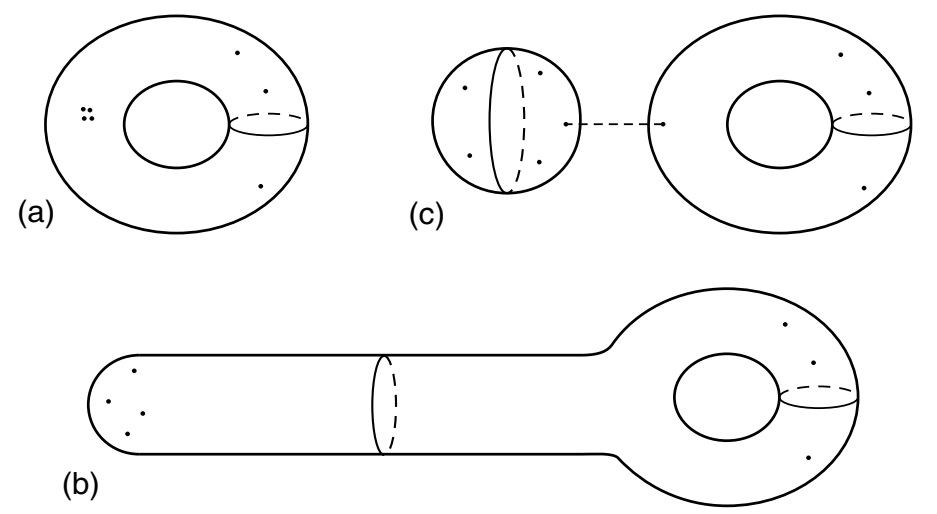
\includegraphics[width=0.8\textwidth]{figure/Fig9.8.jpg}\\
		\caption{(a) A torus with $n$ vertex operators, where $m$ are clustered together. (b) Conformally equivalent image: these $m$ vertex operators are at the end of a long cylinder. 
			(c) Sewing construction, represented as the product of a sphere with $m{+}1$ vertex operators and a torus with $n{-}m{+}1$ vertex operators.}\label{Fig9.8}
	\end{center}
\end{figure}

Before moving forward, we provide further explanation that string divergences are long-range.
Consider a one-loop amplitude with $n$ vertex operators, keeping $\tau$ fixed, and taking the limit where $m$ operators cluster together, as shown in Figure \ref{Fig9.8}. 
String loops certainly contain gravity, and when interactions cluster in spacetime, this has UV divergence. There is indeed a divergence in this string amplitude, but it comes from long-range spacetime distances, not short-range. 
Figure \ref{Fig9.8}b gives a conformally equivalent description, where $m$ vertex operators are connected to the remaining torus through a long cylinder.
Cutting the cylinder and inserting a complete set of states, 
we obtain the usual representation \eqref{9.5.2}, where $q \rightarrow 0$ becomes the limit of vertex operator clustering. So the only singularity is the pole of the propagator at long-range spacetime. 
Conformal invariance once again transforms short-range on the world-sheet into long-range in spacetime.

The cases $m=n$ and $m=n{-}1$ present special problems. When $m=n$, this means all vertex operators cluster together, and momentum conservation makes $k^{\mu}$ zero.
For massless states, the pole is $1/0$, 
and since momentum conservation forces the amplitude to stay on the pole, analytic continuation does not help. This is a tadpole diagram, as in Section \ref{sec:7.4}, and the solution is the same: corrections to the background field. 
The divergence here is proportional to the torus amplitude with one vertex operator.

Another problematic case is $m=n-1$, where all vertex operators cluster together except for one vertex operator $\mathscr{V}_{n}$. 
Momentum conservation requires the momentum flowing through the cylinder to be $k^{\mu}=-k_{n}^{\mu}$.
However, conformal invariance requires $k_{n}^{2}=-m_{n}^{2}$, so for those intermediate states with $m_{j}^{2}=m_{n}^{2}$, 
the momentum of the intermediate state is fixed at the top of a pole, as shown in Figure \ref{Fig9.9}: the intermediate propagator is $1/0$. As long as the internal line $j$ is the same as the external line $n$, divergence occurs. 
The explanation is quite simple. This loop represents a radiative correction to the mass of particle $n$. Define the S-matrix's external momentum as being on the true mass shell, which includes radiative corrections, and this still does not have this IR divergence.
Note that the problem here is not the UV divergence within the loop, but the IR divergence of the starred propagator, which happens even if the mass correction is finite. 
The solution in the string case is the same. The momentum appearing in the vertex operators must be at the true physical mass; in general, they are not the same as the tree-level mass, 
which are integer multiples of $1 / \alpha^{\prime}$. Note that for certain massless fields—especially gauge bosons—gauge invariance requires them to be massless to all orders.
Incidentally, for massive states, the mass shift is usually complex; these states are unstable and will decay to light string states.

\begin{figure}[!htbp]
	\begin{center}
		%width=0.8\textwidth,bb=0 0 435 233
		%1px=0.75pt
		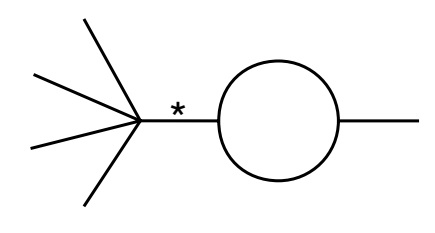
\includegraphics[width=0.8\textwidth]{figure/Fig9.9.jpg}\\
		\caption{Field theory diagram corresponding to the case $m=n{-}1$. Kinematics forces the starred propagator to diverge. The solution is the (finite) mass shift due to the loop.}\label{Fig9.9}
	\end{center}
\end{figure}


There is a question here. Earlier, when we studied the compatibility of string theory, world-sheet conformal invariance required the $\beta$-function \eqref{3.7.14} to be zero. 
These $\beta$-functions do not include information about high genus surfaces—they correspond to tree-level string field equations. What happens when we try to expand around the loop-corrected background? 
In fact, all problems are solved. The dangerous limits in Figure \ref{Fig9.8} give not only divergence but also conformal anomalies.
To see this, 
draw this limit as in \ref{Fig9.3}c, with a small handle glued onto the sphere. This small handle can be represented by a series of local operators; in particular, from the massless level there is:
\begin{equation}
	\partial X^{\mu} \bar{\partial} X_{\mu} \frac{\dif q \dif \bar{q}}{q \bar{q}} \:. \label{9.5.4}
\end{equation}
Now by requiring the size of the handle to be greater than $a$; that is, $|q|
\me^{\omega}>a$, where the metric on the sphere is $\dif z \dif \bar{z} \me^{2 \omega}$,  
the divergence is cut off in a coordinate-invariant way. The lower bound of the integral \eqref{9.5.4} gives:
\begin{equation}
	-4 \pi \partial X^{\mu} \bar{\partial} X_{\mu} \ln (a \me^{-\omega}) \:.
	\label{9.5.5}
\end{equation}
\begin{tcolorbox}[breakable]
	\begin{remark}
		With $q=r\me^{\mi\theta}$ and $\dif^2q=2r\,\dif r\,\dif\theta$, the handle integral runs over $a\me^{-\omega}<|q|<1$:
		\begin{equation*}
			\int_{a\me^{-\omega}<|q|<1}\frac{\dif^2q}{q\bar q}\eqs{1}2\int_0^{2\pi}\dif\theta\int_{a\me^{-\omega}}^1\frac{\dif r}{r}\eqs{2}-4\pi\ln\bigl(a\me^{-\omega}\bigr)=-4\pi\ln a+4\pi\omega .
		\end{equation*}
		At (1) $q\bar q=r^2$. At (2) the angular integral gives $2\pi$ and the radial one $-\ln(a\me^{-\omega})$. Multiplying by $\partial X^\mu\bar\partial X_\mu$ gives \eqref{9.5.5}. The dependence on the cutoff is logarithmic, and the piece $4\pi\omega\,\partial X\cdot\bar\partial X$ is an explicit dependence on the Weyl factor. It has the form of a shift of the metric coupling $\eta_{\mu\nu}\partial X^\mu\bar\partial X^\nu$, so it contributes a term proportional to $\eta_{\mu\nu}$ to $\beta^G_{\mu\nu}$.
	\end{remark}
\end{tcolorbox}
Thus, the Weyl factor of our metric has a new dependence: this corrects the Weyl anomaly $\beta_{\mu v}^{G}$ of the $\sigma$-model, \eqref{3.7.14}. 
To obtain a Weyl-invariant theory, the background must satisfy the full string loop-corrected Weyl invariance condition (or equivalently, BRST invariance). 
The Weyl anomaly from the offset background cancels the anomaly from the small handle, which is the Fischler-Susskind mechanism. From Figure \ref{Fig9.3}c, we can consider divergence and Weyl anomaly as world-sheet UV effects, 
which do not come from the usual short-wave fluctuations of fields, but from very small topological fluctuations. We should emphasize that for any fixed Riemann surface of any genus, the local structure is not affected by topology; 
what generates divergence and Weyl anomaly is the integration over Riemann surfaces.
This can also be considered as the failure of the cancellation of propagator discussion. Kinematics forces the amplitude to stay on the pole, and we cannot use analytic continuation to eliminate possible surface terms under BRST variation. 
In fact, their appearance corresponds to the Weyl anomaly \eqref{9.5.5}. In the loop-corrected background, the BRST anomaly from the background offset cancels the BRST anomaly generated by the moduli space boundary—assembling the string characteristics together gives a consistent spacetime picture.

Implementing this in string perturbation theory is quite cumbersome, but fortunately, it is rarely necessary. First, in most supersymmetric theories, the background is not corrected. 
Second, in string theory, it is most efficient to analyze long-range physics in two steps: first use string theory to derive the form of the low-energy effective action, and then use this theory for long-range. 
Then, we do not need to deal with IR divergence at the string theory level.
In the current case, the tadpole diagram gives the following potential energy term:
\begin{equation}
	\delta \bm{S}=-\sum_{\chi} \Lambda_{\chi} \int \dif^{d} x \: (-G)^{1/2} \me^{-\chi \Phi} \:. \label{9.5.6}
\end{equation}
Here $\Lambda_{\gamma}$ comes from the Euler number, and the dependence of the action on $\Phi$ comes from the fact that $\me^{\Phi}$ is the string coupling. 
After some effort, we can extract individual tadpole diagrams of gravitons and dilatons from string amplitudes.
The same concept extends to vertex operator corrections from mass shifts, and other IR divergences, for example, exclusive amplitudes in theories with massless particles. Since string theory degenerates into field theory at long-range, 
these field theory divergences must also appear in the corresponding string amplitudes. We emphasize again that UV divergences in field theory generally indicate basic limits to the theory's applicability, while IR divergences usually mean the wrong question was asked. 
Any such divergence is treated in string theory in the same way as in field theory.

Let's review what we have learned. For the specific moduli problem of bosonic strings, the S-matrix is finite and unitary. The basic mechanism is modular invariance, which cuts off UV divergence without breaking spacetime gauge invariance. 
Of course, knowing that string theory is reasonable in weak coupling perturbation theory around flat spacetime is far from enough.
We hope to know whether this theory is still reasonable beyond perturbation theory, and to have some means of calculating non-perturbative corrections. 
Additionally, we hope to know what string theory implies for the short-range properties of spacetime. In the rest of this chapter, we will briefly describe attempts in these directions.

\section{String field theory} \label{sec:9.6}

It is very interesting to compare the methods we use in string theory with those for constructing quantum field theories. World-sheet path integrals are similar to summing over particle paths, which is usually called the first quantization scheme. On the other hand, in quantum field theory, we can develop quantum field theory in the first quantization form, where interaction vertices must be introduced, i.e., where several particles cluster.
In string theory, the second step is unnecessary—there are no special points, and the sum over topologies generates the interactions. 
However, this result is just a perturbation expansion, and some phenomena will not appear in this expansion. In the Standard Model, this includes quark confinement and finite-temperature baryon number violation in weak interactions. 
There seems to be no way to make them appear in the resummed perturbation expansion; instead, they require a more general construction of the theory.

In the previous section, we expressed string amplitudes in the form of propagators and vertices, much like the perturbation theory of infinite-component field theories. 
Can we derive this form from an integration over an infinite set of spacetime fields? Are there some principles, extending gauge invariance and general coordinate invariance, that determine the form of the theory? 
This is the subject of string field theory.
We start from the following assumption: take the string wavefunction $\Psi[X]$ and promote it to a field operator, or equivalently a path integral variable—this is the so-called second quantization. 
Now, $\Psi[X]$ depends on the curve $X^{\mu}(\sigma)$ described by the string in spacetime. Roughly speaking, a string is created or annihilated in this configuration. 
However, we need to be more precise: should we require $\Psi$ to be invariant under reparametrization of the curve? And does it also depend on the Polyakov metric $g_{ab}$?
If we start from the BRST form of the theory, introduce Faddeev-Popov ghosts, and then second-quantize, everything seems fine. 
From the commutation relations, $b$ and $c$ are conjugate to each other, so if we consider $c$ and $\tilde{c}$ as coordinates, and the wavefunction is $\Psi[X, c, \tilde{c}]$, 
then we have a path integral over all these functionals:
\begin{equation}
	\int[\dif \Psi] \: \exp (\mi S[\Psi]) \:.
	\label{9.6.1}
\end{equation}
We first examine open strings and describe a specific approach. 

What symmetry will constrain the string action? From our study of string vertex operators and null states, we might guess it is the symmetry:
\begin{equation}
	\delta \Psi=Q_{\mathrm{B}} \Lambda \label{9.6.2}
\end{equation}
where $\Lambda$ is an arbitrary functional. The simplest action with this invariance is:
\begin{equation}
	S_{0}=\frac{1}{2}\lAngle\Psi |Q_{\mathrm{B}}| \Psi\rangle \:. \label{9.6.3}
\end{equation}
The equations of motion are:
\begin{equation}
	Q_{\mathrm{B}} \Psi=0 \:. \label{9.6.4}
\end{equation}
\begin{tcolorbox}[breakable]
	\begin{remark}
		Conventions. $\lAngle A|B\rangle$ is the BPZ inner product on the disk, which is nonzero only for total ghost number $3$. $Q_{\mathrm B}$ is BPZ-odd up to a sign, $\lAngle Q_{\mathrm B}A|B\rangle=\pm\lAngle A|Q_{\mathrm B}B\rangle$ (contour deformation on the sphere), and the pairing is symmetric on the ghost-number-1 fields used here. The field $\Psi$ has ghost number 1, like $c\mathscr V$, and $\Lambda$ has ghost number 0. The action \eqref{9.6.3} has total ghost number $1+1+1=3$. Varying,
		\begin{align*}
			\delta S_0&=\frac12\Bigl(\lAngle\delta\Psi|Q_{\mathrm B}|\Psi\rangle+\lAngle\Psi|Q_{\mathrm B}|\delta\Psi\rangle\Bigr)\eqs{1}\lAngle\delta\Psi|Q_{\mathrm B}|\Psi\rangle ,\\
			\delta_\Lambda S_0&=\lAngle Q_{\mathrm B}\Lambda|Q_{\mathrm B}|\Psi\rangle\eqs{2}\pm\lAngle\Lambda|Q_{\mathrm B}^2|\Psi\rangle=0 .
		\end{align*}
		At (1) the symmetry of the quadratic form was used. At (2) $Q_{\mathrm B}$ was moved across and $Q_{\mathrm B}^2=0$. The first line holds for arbitrary $\delta\Psi$, and the BPZ pairing is nondegenerate, so the equation of motion is $Q_{\mathrm B}\Psi=0$. That is the physical-state condition, and the gauge freedom $\Psi\to\Psi+Q_{\mathrm B}\Lambda$ is the BRST-null equivalence. Solutions modulo gauge are therefore the BRST cohomology at ghost number 1.
	\end{remark}
\end{tcolorbox}

One way to see its rationality is to expand the string field $\Psi$ into infinitely many ordinary fields, each corresponding to an internal state of the string.
Let $\Psi_{i}[X^{\prime}, c, \tilde{c}]$ be a complete basis of wavefunction for all internal modes except the center of mass $x^{\mu}$. Then a general state can be expressed as:
\begin{equation}
	\Psi[X, c, \tilde{c}]=\sum_{i} \Phi_{i}(x) \Psi_{i}[X^{\prime}, c, \tilde{c}] \:, \label{9.6.5}
\end{equation}
where the expansion coefficients are functions of the remaining variables $x^{\mu}$.
The path integral of the string field becomes an infinite product of the path integrals of the component functions:
\begin{equation}
	\int[\dif \Psi] \rightarrow \prod_{i} \int[\dif \Phi_{i}] \:. \label{9.6.6}
\end{equation}
As usual, we can start from the ground state functional $\Psi_{0}$ and use raising operators to build the remaining states.
For example, keeping only the states of the first two levels:
\begin{align}
	\Psi &= \Bigl[\varphi(x) + A_{\mu}(x) \alpha_{-1}^{\mu} + B(x) b_{-1} + C(x) c_{-1} + \varphi^{\prime}(x) c_{0}\nonumber \\
	&\qquad+A_{\mu}^{\prime}(x) \alpha_{-1}^{\mu} c_{0} + B^{\prime}(x) b_{-1} c_{0} + C^{\prime}(x) c_{-1} c_{0} + \cdots\Bigr] 
	\Psi_{0} \:.
	\label{9.6.7}
\end{align}
Here $\varphi$ is the tachyon field, $A_{\mu}$ is the gauge field, and $B$ and $C$ are the Faddeev-Popov ghost fields corresponding to spacetime gauge symmetry. 
The primed fields can always be gauged away, or they are auxiliary fields (i.e., they satisfy algebraic equations rather than differential equations and can be eliminated). 
The symmetry \eqref{9.6.2} can be verified to include the ordinary gauge transformation on $A_{\mu}$, while the action for $\varphi$ is in the Klein-Gordon form and for $A_{\mu}$ is in the Maxwell form. 
Thus BRST string field theory gives a very compact extension of spacetime gauge invariance.
\begin{tcolorbox}[breakable]
	\begin{remark}
		Conventions (Polchinski Ch.~4). Open string, $\Psi_0=|{\downarrow};k\rangle=c_1|0;k\rangle$ with $|0\rangle$ the $SL(2)$ vacuum, $\alpha_0^\mu=(2\alpha')^{1/2}k^\mu$, and $L_0^{\mathrm m}=\alpha'k^2+N$. The BRST charge is $Q_{\mathrm B}=\sum_nc_nL^{\mathrm m}_{-n}+(\text{ghost terms})$, and it annihilates $|0;0\rangle$. The BPZ map (open string, $u=-1/z$) sends a weight-$h$ mode $\phi_n\to(-1)^{n+h}\phi_{-n}$; the normalization $\mathcal K\equiv\langle0|c_{-1}c_0c_1|0\rangle$ is left as a convention. Keep the ghost-number-1 part of \eqref{9.6.7} at levels $0$ and $1$. Since $b_{-1}c_0\Psi_0=-c_0b_{-1}c_1|0\rangle=-c_0|0\rangle$, write $\beta\equiv-B'$:
		\begin{equation*}
			\Psi=\bigl[\varphi\,c_1+A_\mu\,\alpha^\mu_{-1}c_1+\beta\,c_0\bigr]|0;k\rangle ,\qquad \Lambda=\lambda\,b_{-1}\Psi_0=\lambda|0;k\rangle .
		\end{equation*}
		\emph{Gauge transformation.} Only the matter Virasoro modes feel the momentum, and only $c_0,c_1$ survive on $|0\rangle$:
		\begin{equation*}
			Q_{\mathrm B}\Lambda\eqs{1}\lambda\bigl(c_0L_0^{\mathrm m}+c_1L_{-1}^{\mathrm m}\bigr)|0;k\rangle\eqs{2}\lambda\bigl[\alpha'k^2\,c_0+(2\alpha')^{1/2}k\cdot\alpha_{-1}\,c_1\bigr]|0;k\rangle ,
		\end{equation*}
		so $\delta A_\mu=(2\alpha')^{1/2}k_\mu\lambda$ and $\delta\beta=\alpha'k^2\lambda$. At (1) the $k=0$ terms reproduce $Q_{\mathrm B}|0;0\rangle=0$, $c_{n\ge2}|0\rangle=0$, and $L^{\mathrm m}_{n\ge1}|0;k\rangle=0$. At (2) $L^{\mathrm m}_{-1}|0;k\rangle=\alpha_{-1}\cdot\alpha_0|0;k\rangle$. With $k\to-\mi\partial$ this is $\delta A_\mu\propto\partial_\mu\lambda$, the Maxwell gauge transformation.

		\emph{Action on each component.} The ghost pieces follow from $\{Q_{\mathrm B},c_p\}=\sum_{m+n=p}(1-n)c_mc_n$ (the mode form of $\delta c=c\partial c$) and $[Q_{\mathrm B},\alpha^\mu_{-1}]=\sum_nc_n\alpha^\mu_{-1-n}$. On $|0\rangle$ they give $\{Q_{\mathrm B},c_1\}|0\rangle=-c_0c_1|0\rangle$ and $\{Q_{\mathrm B},c_0\}|0\rangle=-2c_{-1}c_1|0\rangle$. Therefore
		\begin{align*}
			Q_{\mathrm B}\,c_1|0;k\rangle&\eqs{3}\bigl(\alpha'k^2-1\bigr)c_0c_1|0;k\rangle,\\
			Q_{\mathrm B}\,\alpha^\mu_{-1}c_1|0;k\rangle&\eqs{4}\alpha'k^2\,\alpha^\mu_{-1}c_0c_1|0;k\rangle+(2\alpha')^{1/2}k^\mu\,c_{-1}c_1|0;k\rangle,\\
			Q_{\mathrm B}\,c_0|0;k\rangle&\eqs{5}-2\,c_{-1}c_1|0;k\rangle-(2\alpha')^{1/2}k\cdot\alpha_{-1}\,c_0c_1|0;k\rangle .
		\end{align*}
		At (3) $Q_{\mathrm B}c_1=\{Q_{\mathrm B},c_1\}-c_1Q_{\mathrm B}$ and the result for $Q_{\mathrm B}|0;k\rangle$ were used. At (4) $[Q_{\mathrm B},\alpha_{-1}]$ contributes $c_0\alpha_{-1}+c_{-1}\alpha_0$, and the $-1$ of (3) cancels the $+1$ from $N=1$. At (5) $Q_{\mathrm B}c_0=\{Q_{\mathrm B},c_0\}-c_0Q_{\mathrm B}$ was used. So
		\begin{equation*}
			Q_{\mathrm B}\Psi=\varphi(\alpha'k^2-1)c_0c_1|0\rangle+\bigl[\alpha'k^2A_\mu-(2\alpha')^{1/2}k_\mu\beta\bigr]\alpha^\mu_{-1}c_0c_1|0\rangle+\bigl[(2\alpha')^{1/2}k\cdot A-2\beta\bigr]c_{-1}c_1|0\rangle ,
		\end{equation*}
		which is invariant under the gauge transformation above: $\alpha'k^2(2\alpha')^{1/2}k\lambda-(2\alpha')^{1/2}k\,\alpha'k^2\lambda=0$ and $2\alpha'k^2\lambda-2\alpha'k^2\lambda=0$.

		\emph{Action.} The BPZ bras are $\langle0;-k|c_{-1}$, $\langle0;-k|\alpha^\nu_1c_{-1}$, and $-\langle0;-k|c_0$. Their only nonzero pairings are
		\begin{equation*}
			\langle0|c_{-1}\,c_0c_1|0\rangle=\mathcal K,\qquad\langle0|\alpha_1^\nu c_{-1}\,\alpha^\mu_{-1}c_0c_1|0\rangle=\eta^{\mu\nu}\mathcal K,\qquad-\langle0|c_0\,c_{-1}c_1|0\rangle=\mathcal K ,
		\end{equation*}
		so all three components are weighted by the same $\mathcal K$. The string-field reality condition makes $\varphi,A_\mu$ real and $\beta=\mi B$ with $B$ real. That is what makes the cross term real in position space, where $k\cdot A(-k)\beta(k)\to\mi B\,\partial\cdot A$ up to sign. Then, with $k\to-\mi\partial$,
		\begin{align*}
			S_0&=\frac{\mathcal K}{2}\int\dif^dx\Bigl[\alpha'\partial\varphi\cdot\partial\varphi-\varphi^2+\alpha'\partial_\nu A_\mu\partial^\nu A^\mu+2(2\alpha')^{1/2}B\,\partial\cdot A+2B^2\Bigr]\\
			&\eqs{6}\frac{\mathcal K\alpha'}{2}\int\dif^dx\Bigl[\partial\varphi\cdot\partial\varphi-\frac{1}{\alpha'}\varphi^2+\partial_\nu A_\mu\partial^\nu A^\mu-(\partial\cdot A)^2\Bigr]\\
			&\eqs{7}\frac{\mathcal K\alpha'}{2}\int\dif^dx\Bigl[\partial\varphi\cdot\partial\varphi+m^2\varphi^2+\frac12F_{\mu\nu}F^{\mu\nu}\Bigr],
		\end{align*}
		with $m^2=-1/\alpha'$. At (6) the auxiliary field was eliminated by its algebraic equation $B=-\frac12(2\alpha')^{1/2}\partial\cdot A$, which turns $2(2\alpha')^{1/2}B\,\partial\cdot A+2B^2$ into $-\alpha'(\partial\cdot A)^2$. At (7) an integration by parts was used. Choosing $\mathcal K=-1/\alpha'$ gives the canonical Klein--Gordon action for the open-string tachyon and the Maxwell action $-\frac14F^2$.
	\end{remark}
\end{tcolorbox}
\begin{figure}[!htbp]
	\begin{center}
		%width=0.8\textwidth,bb=0 0 840 261
		%1px=0.75pt
		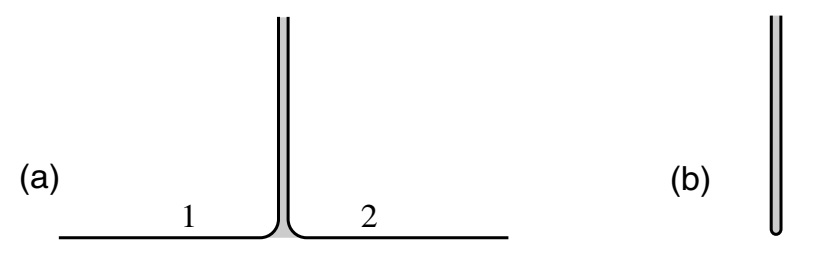
\includegraphics[width=0.8\textwidth]{figure/Fig9.10.jpg}
		\caption{(a) $\Psi_{1} * \Psi_{2}$, the convolution of the right half of $\Psi_{1}$ and the left half of $\Psi_{2}$. This can be considered as defining a path integral for the shaded region, later taking the limit where the width of this region tends to zero. (b) $\int \Psi$, the convolution of the right half and left half of $\Psi$.}\label{Fig9.10}
	\end{center}
\end{figure}
\vspace*{-0.7cm}

There is no problem in solving for interactions. Define the product operation $\Psi_{1} * \Psi_{2}$ on string fields through the functional integral shown in Figure \ref{Fig9.10}a, 
formed by overlapping the right side of $\Psi_{1}$ and the left side of $\Psi_{2}$.
Also define $\int$, which gives the overlap of the right side and left side of a single string wavefunction as shown in Figure \ref{Fig9.10}b. 
To provide an interactive theory, add non-linear terms to the gauge transformation:
\begin{equation}
	\delta \Psi=Q_{\mathrm{B}} \Lambda+g \Psi * \Lambda-g \Lambda * \Psi \:.
	\label{9.6.8}
\end{equation}
The $*$ product is associative, and through a contour discussion, it can be proven that $Q_{\mathrm{B}}$ acts like a derivative:
\begin{equation}
	Q_{\mathrm{B}}(\Psi_{1} * \Psi_{2})=(Q_{\mathrm{B}} \Psi_{1}) * \Psi_{2}+\Psi_{1} *(Q_{\mathrm{B}} \Psi_{2}) \:. \label{9.6.9}
\end{equation}
From these it follows that \eqref{9.6.8} is closed.
Using cyclicity:
\begin{equation}
	\int \Psi_{1} * \Psi_{2}=\int \Psi_{2} * \Psi_{1} \:, \label{9.6.10}
\end{equation}
we can write down the invariant action:
\begin{equation}
	S=\frac{1}{2} \int \Psi * Q_{\mathrm{B}} \Psi + \frac{2 g}{3} \int \Psi * \Psi * \Psi \:.
	\label{9.6.11}
\end{equation}
\begin{tcolorbox}[breakable]
	\begin{remark}
		Conventions (Witten's cubic theory). Signs are graded by ghost number: $\Psi$ is odd, $\Lambda$ is even, and $Q_{\mathrm B}$ is odd. The rules are
		\begin{gather*}
			Q_{\mathrm B}(A*B)=(Q_{\mathrm B}A)*B+(-1)^{|A|}A*(Q_{\mathrm B}B),\\
			\int Q_{\mathrm B}(\cdots)=0,\qquad\int A*B=(-1)^{|A||B|}\int B*A .
		\end{gather*}
		These are the graded forms of \eqref{9.6.9}, of the vanishing of a total BRST variation on the disk, and of \eqref{9.6.10}. To keep track of the relative normalization, write the action as $S=\frac12\int\Psi*Q_{\mathrm B}\Psi+\kappa\int\Psi*\Psi*\Psi$ and the gauge transformation as $\delta\Psi=Q_{\mathrm B}\Lambda+g'(\Psi*\Lambda-\Lambda*\Psi)$.

		\emph{Gauge invariance.} First, $\delta\frac12\int\Psi*Q\Psi=\int\delta\Psi*Q\Psi$ and $\delta\,\kappa\int\Psi^{*3}=3\kappa\int\delta\Psi*\Psi*\Psi$, both by cyclicity. Define $\mathcal I\equiv\int\Lambda*Q\Psi*\Psi-\int\Lambda*\Psi*Q\Psi$. Order by order in the coupling:
		\begin{align*}
			\mathcal O(g^0):&\quad\int Q\Lambda*Q\Psi\eqs{1}\int Q(\Lambda*Q\Psi)=0,\\
			\mathcal O(g^1):&\quad g'\!\int(\Psi*\Lambda-\Lambda*\Psi)*Q\Psi+3\kappa\int Q\Lambda*\Psi*\Psi\eqs{2}g'\,\mathcal I+3\kappa(-\mathcal I)=(g'-3\kappa)\,\mathcal I,\\
			\mathcal O(g^2):&\quad 3\kappa g'\Bigl(\int\Psi*\Lambda*\Psi*\Psi-\int\Lambda*\Psi*\Psi*\Psi\Bigr)\eqs{3}0 .
		\end{align*}
		At (1) $Q^2=0$ and the Leibniz rule were used. At (2) cyclicity gives $\int\Psi*(\Lambda*Q\Psi)=\int\Lambda*Q\Psi*\Psi$, and the Leibniz rule with $\int Q(\Lambda*\Psi*\Psi)=0$ gives $\int Q\Lambda*\Psi*\Psi=-\int\Lambda*Q\Psi*\Psi+\int\Lambda*\Psi*Q\Psi=-\mathcal I$. At (3) the odd $\Psi$ was moved cyclically past $\Lambda*\Psi*\Psi$, which has even degree $0+1+1$, so no sign appears and the two terms cancel. Invariance therefore requires
		\begin{equation*}
			\boxed{g'=3\kappa} .
		\end{equation*}
		With the gauge transformation \eqref{9.6.8} as printed ($g'=g$) the cubic coefficient must be $\kappa=g/3$, which is Witten's normalization $S=\frac12\int\Psi*Q\Psi+\frac g3\int\Psi*\Psi*\Psi$. With the action \eqref{9.6.11} as printed ($\kappa=2g/3$) the gauge transformation must be $\delta\Psi=Q\Lambda+2g(\Psi*\Lambda-\Lambda*\Psi)$. The printed pair is off by a factor of 2 in one of the two places. This is only a normalization of $g$ and does not affect any conclusion.

		\emph{Closure.} Write $[\Psi,\Lambda]\equiv\Psi*\Lambda-\Lambda*\Psi$, so $\delta_\Lambda\Psi=Q\Lambda+g'[\Psi,\Lambda]$. Then
		\begin{align*}
			[\delta_1,\delta_2]\Psi&=g'\bigl([Q\Lambda_1,\Lambda_2]-[Q\Lambda_2,\Lambda_1]\bigr)+g'^2\bigl([[\Psi,\Lambda_1],\Lambda_2]-[[\Psi,\Lambda_2],\Lambda_1]\bigr)\\
			&\eqs{4}Q\bigl(g'[\Lambda_1,\Lambda_2]\bigr)+g'\bigl[\Psi,g'[\Lambda_1,\Lambda_2]\bigr]=\delta_{\Lambda_{12}}\Psi,\qquad\Lambda_{12}=g'[\Lambda_1,\Lambda_2] .
		\end{align*}
		At (4) the Leibniz rule gives $Q[\Lambda_1,\Lambda_2]=[Q\Lambda_1,\Lambda_2]+[\Lambda_1,Q\Lambda_2]$ with $[\Lambda_1,Q\Lambda_2]=-[Q\Lambda_2,\Lambda_1]$, and associativity of $*$ gives the Jacobi identity for the second bracket. So the algebra closes, which is the sense in which \eqref{9.6.8} is ``closed''.
	\end{remark}
\end{tcolorbox}
It is usually useful to write it in CFT form, replacing $\Psi$ with the semi-disk corresponding to the vertex operator $\mathscr{V}_{\Psi}$:
\begin{equation}
	S=\frac{1}{2}\langle\mathscr{V}_{\Psi} \,Q_{\mathrm{B}} \cdot \mathscr{V}_{\Psi}\rangle_{D_{2}} + 
	\frac{2 g}{3}\langle\mathscr{V}_{\Psi} \mathscr{V}_{\Psi} \mathscr{V}_{\Psi}\rangle_{D_{2}} \:. \label{9.6.12}
\end{equation}
The vertex operator positions and conformal coordinates are not as marked in \eqref{9.6.12}, but as shown in Figure \ref{Fig9.11}.
A $z^{2 / 3}$ mapping reshapes the trilinear vertex semi-disk into a disk. 
This action passes a very important test. Only for insertions with a total $Q^{g}=3$, the path integral on the disk is non-zero. The vertex operators for physical states all have ghost number 1, so both terms in \eqref{9.6.12} are non-zero. 
Since \eqref{9.6.11} is invariant, we expect it to reduce to the non-Abelian Yang-Mills action for gauge fields, which indeed it does.


The Siegel gauge is $b_{0} \Psi=0 $.
In the kinetic action, only the $c_{0} L_{0}$ term in $Q_{\mathrm{B}}$ survives. 
Since in components $L_{0} \propto p^{2}+m^{2}$, this is similar to the familiar covariant gauge in electrodynamics.
The propagator:
\begin{equation}
	\int_{0}^{\infty} \dif t \: \exp (-t L_{0}) = L_{0}^{-1} \label{9.6.13}
\end{equation}
\begin{tcolorbox}[breakable]
	\begin{remark}
		Split the BRST charge by ghost zero modes, $Q_{\mathrm B}=c_0L_0+b_0\mathcal M+\hat Q$. Here $\mathcal M$ and $\hat Q$ contain neither $b_0$ nor $c_0$, and $\mathcal M$ is built from $c_{-n}c_n$ with $n\ne0$. In Siegel gauge $b_0\Psi=0$, so $\Psi$ contains no $c_0$. The BPZ product on the disk needs exactly one $c_0$ to saturate the zero mode ($\langle{\downarrow}|c_0|{\downarrow}\rangle\neq0$, $\langle{\downarrow}|{\downarrow}\rangle=0$). Then
		\begin{equation*}
			\lAngle\Psi|Q_{\mathrm B}|\Psi\rangle\eqs{1}\lAngle\Psi|c_0L_0|\Psi\rangle+\lAngle\Psi|\mathcal Mb_0|\Psi\rangle+\lAngle\Psi|\hat Q|\Psi\rangle\eqs{2}\lAngle\Psi|c_0L_0|\Psi\rangle .
		\end{equation*}
		At (1) $b_0\mathcal M=\mathcal Mb_0$, since $b_0$ anticommutes with each $c_{\pm n}$ ($n\ne0$). At (2) the middle term vanishes by $b_0\Psi=0$, and the last one has no $c_0$ at all. The kinetic operator is therefore $c_0L_0$, and on the gauge slice the propagator is $b_0L_0^{-1}$. For $L_0>0$, $L_0^{-1}=\int_0^\infty\dif t\,\me^{-tL_0}$, and elsewhere this is defined by continuation as in \eqref{9.1.22}. Since $L_0$ is the open-string world-sheet Hamiltonian, $\me^{-tL_0}$ is the path integral over a strip of length $t$, and the propagator is the integral over all strip lengths. In components $L_0=\alpha'(k^2+m^2)$, the analogue of Feynman gauge.
	\end{remark}
\end{tcolorbox}
is simply the integral over strips of arbitrary length. The vertex is as shown in Figure \ref{Fig9.11}b where the wedges are removed, and the ends of three strips are inserted into a `$\mathsf{Y}$'.
It has been proven that this is equivalent to the open string theory described by a sum over Riemann surfaces, specifically, this sum includes a complete single-cover of the moduli space. 
On the other hand, this is not unexpected: string field theory has spacetime gauge invariance \eqref{9.6.8}, which makes null states decouple from the S-matrix.
We have argued that the decoupling of null states determines the form of string amplitudes, which includes the requirement for a single-cover of the moduli space (otherwise total derivative terms would give null state coupling). 
On the other hand, moduli space is very complex, and only a few have explicit descriptions. The moduli spaces generated by this string field theory, written as a sum over Feynman diagrams with each diagram being an integral over strip lengths, 
were discovered by physicists only slightly earlier than by mathematicians.\footnote{Another description of moduli space from physics comes from the light-cone gauge, where the moduli are interaction times, 
	the momenta $p^{+}$ of the intermediate states, and the twist angle of each closed string.}


\begin{figure}[!htbp]
	\begin{center}
		%width=0.8\textwidth,bb=0 0 904 352
		%1px=0.75pt
		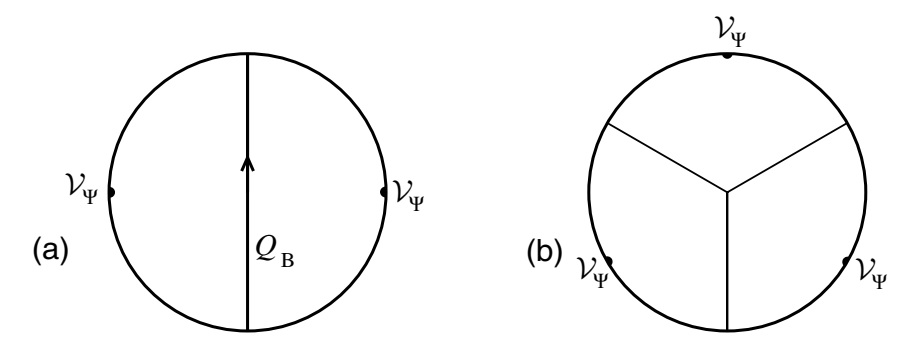
\includegraphics[width=0.8\textwidth]{figure/Fig9.11.jpg}\\
		\caption{CFT representation of the string field action: (a) kinetic term; (b) interaction. A $z^{2/3}$ conformal transformation transforms the usual semi-circle around each vertex operator into the shape of a wedge.}\label{Fig9.11}
	\end{center}
\end{figure}
\vspace*{-0.7cm}

Let's point out a strange feature of this field theory.
We have claimed that string field theory covers the entire moduli space, but we know from the annulus that even without an explicit closed string field, this moduli space will contain the limit that generates closed string poles. 
Closed string poles come from the limit where the strip length tends to zero rather than infinity.\footnote{For this reason, this form of string field theory is not suitable for the purposes of our previous section. We need to add stubs to the vertices to eliminate accidental divergences, 
	and then add closed string propagators and vertices to cover the omitted parts of the moduli space.} The precise statement is that the open string field path integral generates the amplitudes for open string theory plus closed string theory (except for surfaces without any boundaries, which open strings cannot couple to). 
In this sense, in an imprecise way, closed strings are like bound states of open strings.

For theory with only closed strings, we can repeat the above steps with a closed string field, but this will be a bit more complicated. For the free action \eqref{9.6.3}, the ghost number is already insufficient: 
to make matrix elements between physical states non-zero, we need an extra $c$ ghost.
There is a remedy that requires the string field $\Psi$ and gauge transformation $\Lambda$ to be annihilated by $b_{0}-\tilde{b}_{0}$ and $L_{0}-\tilde{L}_{0}$. Then, the action:
\begin{equation}
	S_{0}^{\prime}=\frac{1}{2}\lAngle\Psi |(c_{0}-\tilde{c}_{0}) Q_{\mathrm{B}}| \Psi\rangle \label{9.6.14}
\end{equation}
is invariant under $\delta \Psi=Q_{\mathrm{B}} \Lambda$.
\begin{tcolorbox}[breakable]
	\begin{remark}
		Conventions. Write $b_0^-=b_0-\tilde b_0$, $c_0^-=\frac12(c_0-\tilde c_0)$ and $L_0^-=L_0-\tilde L_0$, so that $\{b_0^-,c_0^-\}=1$ and $\{Q_{\mathrm B},b_0^-\}=L_0^-$. The overall factor of 2 between $c_0-\tilde c_0$ and $c_0^-$ is absorbed in the normalization of $S_0'$. Let $\mathscr H^-$ be the space of states annihilated by $b_0^-$ and $L_0^-$; these states contain no $c_0^-$ excitation.

		\emph{Ghost number.} On the sphere the ghost number must total 6. Closed-string physical fields $\tilde cc\mathscr V$ carry 2, so $\lAngle\Psi|Q_{\mathrm B}|\Psi\rangle$ has $2+1+2=5$ and vanishes identically. The insertion of $c_0^-$ supplies the missing unit: $2+1+1+2=6$.

		\emph{The gauge transformation preserves $\mathscr H^-$.} For $\Lambda\in\mathscr H^-$,
		\begin{equation*}
			L_0^-Q_{\mathrm B}\Lambda=Q_{\mathrm B}L_0^-\Lambda=0,\qquad b_0^-Q_{\mathrm B}\Lambda\eqs{1}\bigl(L_0^--Q_{\mathrm B}b_0^-\bigr)\Lambda=0 ,
		\end{equation*}
		where (1) is $\{Q_{\mathrm B},b_0^-\}=L_0^-$.

		\emph{Invariance.} For $A,B\in\mathscr H^-$ the product $\lAngle A|\mathcal O|B\rangle$ can be nonzero only if $\mathcal O$ contains exactly one $c_0^-$, since neither state does. The operator $\{Q_{\mathrm B},c_0^-\}$ is quadratic in nonzero ghost modes; from $\{Q_{\mathrm B},c_0\}=\sum_mm\,c_mc_{-m}$ and its conjugate, the $m=0$ term vanishes. It therefore contains no $c_0^-$. Then
		\begin{align*}
			\delta S_0'\propto\lAngle Q_{\mathrm B}\Lambda|c_0^-Q_{\mathrm B}|\Psi\rangle
			&\eqs{2}\pm\lAngle\Lambda|Q_{\mathrm B}c_0^-Q_{\mathrm B}|\Psi\rangle
			\eqs{3}\pm\lAngle\Lambda|\bigl(\{Q_{\mathrm B},c_0^-\}-c_0^-Q_{\mathrm B}\bigr)Q_{\mathrm B}|\Psi\rangle\\
			&\eqs{4}\pm\lAngle\Lambda|\{Q_{\mathrm B},c_0^-\}|Q_{\mathrm B}\Psi\rangle\eqs{5}0 .
		\end{align*}
		At (2) $Q_{\mathrm B}$ was moved to the other side of the BPZ product. At (3) the anticommutator was introduced. At (4) $Q_{\mathrm B}^2=0$. At (5) both $\Lambda$ and $Q_{\mathrm B}\Psi$ lie in $\mathscr H^-$ and the operator has no $c_0^-$. The same argument shows that the quadratic form is symmetric, so varying $\Psi$ again gives the equation of motion $Q_{\mathrm B}\Psi=0$ on $\mathscr H^-$. This is precisely the closed-string BRST condition, together with the conditions $(b_0-\tilde b_0)\Psi=(L_0-\tilde L_0)\Psi=0$ of the closed-string BRST analysis in Chapter \ref{cha:4}.
	\end{remark}
\end{tcolorbox}
For an interaction theory, there is no longer an associative product similar to $*$, and correspondingly no single-cover of the moduli space. 
As in the previous section, to cover the moduli space, we need to add higher order vertices $\mathscr{V}_{g, n}$ with higher powers of the field and internal handles. 
Similar to the open string action, the corresponding action can be derived from symmetry principles using the so-called Batalin-Vilkovisky formalism. Then, gauge fixing gives the perturbation theory described in the previous section.

The derivation of string theory from spacetime gauge symmetry is extremely elegant, especially for open strings. Introducing closed strings into open string field theory is very appealing. However, it is not yet known whether string field theory is a useful tool beyond perturbation theory. 
In contemporary non-perturbative developments based on spacetime supersymmetry, string field theory has played no role, and such developments will be discussed in Chapter 14.
It is quite possible that for the non-perturbative construction of ``string theory,'' strings, or string fields, are simply not its correct degrees of freedom.

\section{Large order behavior} \label{sec:9.7}

There is an interesting result about the large order behavior of string perturbation theory. We start with field theory.
Consider the integral:
\begin{equation}
	\int_{-\infty}^{\infty} \dif y \exp \biggl[-\frac{y^{2}}{2!} - \lambda \frac{y^{3}}{3!}\biggr] = 
	\lambda^{-1} \int_{-\infty}^{\infty} \dif z \exp \biggl[-\frac{1}{\lambda^{2}}\biggl(\frac{z^{2}}{2!}+\frac{z^{3}}{3!}\biggr)\biggr] \:,
	\label{9.7.1}
\end{equation}
where $z=y \lambda $.
This integral diverges for $\lambda \neq 0$, but we ignore it for now and compute it as a formal power series in $\lambda$:
\begin{equation}
	\sum_{n=0}^{\infty} \frac{(-\lambda)^{n}}{6^{n} n !} \int_{-\infty}^{\infty} \dif y\: y^{3 n} 
	\exp (-y^{2} / 2) = (2 \pi)^{1 / 2} \sum_{k=0}^{\infty} \lambda^{2 k} C_{2 k} \:, \label{9.7.2}
\end{equation}
where:
\begin{equation}
	C_{2 k}=\frac{2^{k} \Gamma(3 k+1 / 2)}{\pi^{1 / 2} 3^{2 k}(2 k) !} \:.
	\label{9.7.3}
\end{equation}
\begin{tcolorbox}[breakable]
	\begin{remark}
		\emph{Rescaling \eqref{9.7.1}.} With $y=z/\lambda$, $\frac{y^2}{2}+\lambda\frac{y^3}{6}=\frac{1}{\lambda^2}\bigl(\frac{z^2}{2}+\frac{z^3}{6}\bigr)$ and $\dif y=\dif z/\lambda$. So the coupling appears only as an overall $1/\lambda^2$, like $1/\hbar$.

		\emph{Coefficients.} Expand $\exp(-\lambda y^3/6)$ and use $\int\dif y\,y^{2m}\me^{-y^2/2}=2^{m+1/2}\Gamma(m+\frac12)$. Only even powers survive:
		\begin{align*}
			\sum_{n}\frac{(-\lambda)^n}{6^nn!}\int\dif y\,y^{3n}\me^{-y^2/2}
			&\eqs{1}\sum_k\frac{\lambda^{2k}}{6^{2k}(2k)!}\,2^{3k+1/2}\,\Gamma\bigl(3k+\tfrac12\bigr)\\
			&\eqs{2}(2\pi)^{1/2}\sum_k\lambda^{2k}\,\frac{2^{3k}\Gamma(3k+\frac12)}{\pi^{1/2}\,2^{2k}3^{2k}(2k)!} ,
		\end{align*}
		which is \eqref{9.7.3} after $2^{3k}/2^{2k}=2^k$. At (1) odd $n$ vanish by parity, and $n=2k$ gives $m=3k$. At (2) $2^{1/2}=(2\pi)^{1/2}/\pi^{1/2}$ and $6^{2k}=2^{2k}3^{2k}$.

		\emph{Check at $k=1$.} $C_2=\frac{2\,\Gamma(7/2)}{\pi^{1/2}\cdot9\cdot2}=\frac{15/8}{9}=\frac{5}{24}$, using $\Gamma(7/2)=\frac{15}{8}\pi^{1/2}$. The two vacuum graphs with two cubic vertices are the ``theta'' graph (two vertices joined by three lines) and the ``dumbbell'' (two tadpoles joined by a line). Their automorphism groups have orders $2\cdot3!=12$ and $2\cdot2\cdot2=8$, and $\frac1{12}+\frac18=\frac{5}{24}$.
	\end{remark}
\end{tcolorbox}
This integral is the zero-dimensional limit of scalar field theory with a mass term and cubic coupling. The expansion in $\lambda$ can be represented as Feynman diagrams, where the propagator of the diagram is 1 and the vertex is $-\lambda$. 
Thus the constant $C_{2 k}$ counts the total number of vacuum diagrams with $2k$ three-point vertices, which is equivalently the total number of vacuum diagrams with $k+1$ loops, each assigned an appropriate symmetry factor.
For example, the reader can verify that there are two vacuum diagrams with two vertices, with symmetry group orders of 8 and 12, respectively, and $C_{2}=\frac{5}{24}=\frac{1}{8}+\frac{1}{12}$. 
To get the large order behavior, we use Stirling's approximation $n ! \approx n^{n+1 / 2} \me^{-n}$, then:
\begin{equation}
	C_{2 k} \approx k^{k} \approx k !
	\:, \label{9.7.4}
\end{equation}
where the approximation holds up to a factor of the form $k^{a}$ and $b^{k}$.
\begin{tcolorbox}[breakable]
	\begin{remark}
		Stirling's formula $\Gamma(x+1)\approx x^x\me^{-x}$ (dropping powers of $x$) gives
		\begin{equation*}
			C_{2k}\approx\frac{2^k(3k)^{3k}\me^{-3k}}{9^k(2k)^{2k}\me^{-2k}}\eqs{1}\Bigl(\frac{2\cdot27}{9\cdot4}\Bigr)^kk^k\me^{-k}=\Bigl(\frac32\Bigr)^kk^k\me^{-k}\eqs{2}\Bigl(\frac32\Bigr)^k\Gamma(k) .
		\end{equation*}
		At (1) the powers of $k$ and the numerical factors were collected. At (2) $k^k\me^{-k}\approx\Gamma(k)$, again up to powers. So $C_{2k}\approx k!\,b^k$ with $b=\frac32$. The base $b$ has a meaning: the stationary points of $S(z)=\frac{z^2}{2}+\frac{z^3}{6}$ are $z=0$ and $z=-2$, where $S(-2)=2-\frac86=\frac23$. The instanton action is $S(-2)/\lambda^2=2/3\lambda^2$, and the large-order growth is $C_{2k}\sim\Gamma(k)\,[S(-2)]^{-k}$, with $1/S(-2)=\frac32$ exactly the base found above.
	\end{remark}
\end{tcolorbox}

We can also introduce a quartic term $\lambda^{2} y^{4} / 4 !$, which makes the integral converge. The power of $\lambda$ is decided by requiring all terms in the action for $z$ to be proportional to $\lambda^{-2}$; 
or equivalently, all $k+1$ loop vacuum diagrams are assigned a weight $\lambda^{2k}$.
This extra term does not change the result substantially; the estimate \eqref{9.7.4} still holds within certain accuracy.

When considering field theory, propagators and vertices become more complicated. However, the dominant behavior at large orders often comes from the counting of diagrams—unless there is unusual IR or UV behavior, propagators and vertices usually contribute a factor of order $b^{k}$. 
The series takes the following form:
\begin{equation}
	\sum_{k=0}^{\infty} \lambda^{2 k} k !
	f_{2 k} \:, \label{9.7.5}
\end{equation}
where $f_{2 k} \approx k^{a} b^{k}$, which changes much slower than $k!$. Unless there is unexpected cancellation in $f_{2 k}$, this diverges.
For very small $\lambda$, this will be small temporarily, then grow like $k!$. The order of the smallest term in the sum is:
\begin{equation}
	\exp [-O(1 / \lambda^{2})] \:. \label{9.7.6}
\end{equation}
\begin{tcolorbox}[breakable]
	\begin{remark}
		Take $a_k=\lambda^{2k}k!\,f_{2k}$ with $f_{2k}\approx b^k$ (powers of $k$ do not change the estimate). The ratio of successive terms is
		\begin{equation*}
			\frac{a_{k+1}}{a_k}\approx b\lambda^2(k+1)\quad\Longrightarrow\quad a_k\text{ decreases until }k_*\approx\frac{1}{b\lambda^2},
		\end{equation*}
		and the smallest term is
		\begin{equation*}
			a_{k_*}\approx(b\lambda^2)^{k_*}k_*!\eqs{1}(b\lambda^2k_*)^{k_*}\me^{-k_*}\eqs{2}\exp\Bigl(-\frac{1}{b\lambda^2}\Bigr) .
		\end{equation*}
		At (1) Stirling was used. At (2) $b\lambda^2k_*=1$. Truncating the series at its smallest term therefore leaves an irreducible uncertainty of this order. For the example above, $b=\frac32$ gives $\me^{-2/3\lambda^2}$, which is $\me^{-S_{\text{inst}}}$.
	\end{remark}
\end{tcolorbox}
This is the feature of an asymptotic expansion where the accuracy of perturbation theory is limited. Indeed, effects like instantons or dynamical symmetry breaking, which are zero to all orders in perturbation theory, are generally of this order.
For example, the large order behavior of the series \eqref{9.7.2} is related to the instanton (stable point) at $z=-2$, and the instanton action is $2 / 3 \lambda^{2}$.

In string theory, the Feynman diagrammatic decomposition of the moduli space makes it entirely possible to construct the same constraints. For a series of the form \eqref{9.7.5}, where $f_{2 k}$ is positive-definite and has a lower bound $b^{k}$, this has been explicitly proven.
Thus, this series is divergent and not even Borel summable. Borel summation rewrites the series \eqref{9.7.5} as a Laplace transform of another more convergent series:
\begin{equation}
	\int_{0}^{\infty} \dif t\: \exp (-t) \sum_{k=0}^{\infty}(t \lambda^{2})^{k} f_{2 k} \:. \label{9.7.7}
\end{equation}
However, the positive-definiteness of $f_{2 k}$ implies that this new sum, even if convergent, has poles on the positive real axis, so this integral is ill-defined.
\begin{tcolorbox}[breakable]
	\begin{remark}
		The equality of \eqref{9.7.5} and \eqref{9.7.7} term by term is $\int_0^\infty\dif t\,\me^{-t}t^k=k!$. For the model growth $f_{2k}=b^k$,
		\begin{equation*}
			\sum_k(t\lambda^2)^kb^k=\frac{1}{1-b\lambda^2t},
		\end{equation*}
		which has a pole at $t_*=1/b\lambda^2>0$, on the integration contour. Positive $f_{2k}$ always put the nearest singularity on the positive axis. Passing the pole above or below gives results that differ by $2\pi\mi$ times the residue,
		\begin{equation*}
			\Delta=\pm2\pi\mi\,\frac{\me^{-t_*}}{b\lambda^2}=\pm\frac{2\pi\mi}{b\lambda^2}\exp\Bigl(-\frac{1}{b\lambda^2}\Bigr),
		\end{equation*}
		an ambiguity of exactly the size \eqref{9.7.6} of the smallest term. The perturbation series alone does not fix these $\exp[-O(1/\lambda^2)]$ terms.
	\end{remark}
\end{tcolorbox}
Thus, we expect an interesting non-perturbative phenomenon in string theory. This is not surprising since they degenerate to non-trivial field theories in the low-energy limit.

The estimate \eqref{9.7.4} is a lower bound for closed string theory, which can be obtained by only keeping the tree-level trilinear vertex $\mathscr{V}_{0,3}$. 
Since closed string vertices will receive corrections from Riemann surfaces of all genus, we wonder if the perturbation theory will grow even faster. One way to see that it does is to recall that open string field theory contains all open string Riemann surfaces, 
and closed string Riemann surfaces with at least one boundary. Let's examine surfaces with only one boundary, and the moduli space region where the boundary shrinks to a point. 
The limit of the open string moduli space equals the moduli space of a closed surface with one vertex operator. It can be proven that this region is not much smaller than the entire open string moduli space, so the same estimate still holds.
The perturbation series tends to:
\begin{equation}
	\sum_{k=0}^{\infty} g_{\mathrm{o}}^{2 k} O(k !)=\sum_{k=0}^{\infty} g_{\mathrm{c}}^{k} O(k !) \:. \label{9.7.8}
\end{equation}
The term of genus $g$ is proportional to $g_{\mathrm{c}}^{2 g}$, and it has a coefficient of order $(2g)!$.
This is larger than the $g!$ feature of field theory, 
which is also the lower bound obtained only from $\mathscr{V}_{0,3}$. Clearly, the largest part of the high-order amplitudes is contained in the vertex $\mathscr{V}_{g, n}$ and comes from the interior of the moduli space. 
Non-perturbative effects can be expected to be of the order:
\begin{equation}
	\exp [-O(1/g_{\mathrm{c}})] \:, \label{9.7.9}
\end{equation}
\begin{tcolorbox}[breakable]
	\begin{remark}
		Each open-string loop costs $g_{\mathrm o}^2$ and each handle $g_{\mathrm o}^4\propto g_{\mathrm c}^2$, so $g_{\mathrm o}^{2k}=g_{\mathrm c}^{k}$ up to constants, which is \eqref{9.7.8}. Genus $g$ then corresponds to $k=2g$, with coefficient $(2g)!$. Repeating the estimate of \eqref{9.7.6} with $a_k=g_{\mathrm c}^k\,k!\,b^k$:
		\begin{equation*}
			\frac{a_{k+1}}{a_k}\approx bg_{\mathrm c}(k+1)\ \Rightarrow\ k_*\approx\frac{1}{bg_{\mathrm c}},\qquad a_{k_*}\approx(bg_{\mathrm c}k_*)^{k_*}\me^{-k_*}=\exp\Bigl(-\frac{1}{bg_{\mathrm c}}\Bigr).
		\end{equation*}
		The only change from field theory is that $g_{\mathrm c}$ replaces $\lambda^2\sim g_{\mathrm c}^2$ as the expansion parameter multiplying $k!$. So the ambiguity is $\me^{-O(1/g_{\mathrm c})}$, parametrically larger than the field-theory $\me^{-O(1/g_{\mathrm c}^2)}$ at weak coupling.
	\end{remark}
\end{tcolorbox}
which is much larger than the field theory feature $\exp[-O(1 / g_{\mathrm{c}}^{2})]$ at weak coupling. The large order behavior was first observed in some simplified models discussed in Section \ref{sec:9.9}.
We will see in Chapter 13 that these effects are related to D-branes, at least in some superstring theories.


\section{High energy and high temperature} \label{sec:9.8}

To gain a better understanding of string dynamics, we can look at its behavior in different limits. In this section, we examine various high-energy limits of string theory.

\subsection*{Hard scattering}

Again, examine the hard scattering behavior, which is obtained by applying Stirling's approximation to the Veneziano and Virasoro-Shapiro amplitudes.
Returning to the integral form \eqref{6.6.5}:
\begin{equation}
	\frac{8 \pi \mi g_{\mathrm{c}}^{2}}{\alpha^{\prime}} (2\pi)^{26} \delta^{26}({\textstyle \sum_{i} k_{i}}) 
	\int_{\mathds{C}} \dif^{2} z_{4} \: |z_{4}|^{-\alpha^{\prime}u/2 - 4}|1-z_{4}|^{-\alpha^{\prime} t/2 - 4} \:.
	\label{9.8.1}
\end{equation}
In the hard scattering region where $t/s$ is kept fixed and $s \rightarrow \infty$, the exponent is very large, and the integral is dominated by the stationary point of the exponent.\footnote{As usual, the integral diverges as $z_{4}\to \infty$ and is defined by analytic continuation. The reasonableness of the saddle point approximation can be argued by continuation.} When $s, t, u \gg 1$, the saddle point is:
\begin{equation}
	\frac{\partial}{\partial z_{4}}\Bigl(u \ln |z_{4}|^{2}+t \ln |1-z_{4}|^{2}\Bigr) = 
	\frac{u}{z_{4}} + \frac{t}{z_{4}-1} = 0 \:, \label{9.8.2}
\end{equation}
its solution is $z_{4} = -u/s$;
recall that $s+t+u=O(1)$. Then the saddle point approximation gives the amplitude:
\begin{equation}
	S \approx \exp [-\alpha^{\prime}(s \ln s + t \ln t + u \ln u) / 2] \:, \label{9.8.3}
\end{equation}
the same as given by \eqref{6.6.13}.
\begin{tcolorbox}[breakable]
	\begin{remark}
		For large $s,t,u$ the $-4$'s in the exponents of \eqref{9.8.1} are subleading, and the integrand is $\me^{E(z,\bar z)}$ with
		\begin{equation*}
			E=-\frac{\alpha'}{4}\Bigl(u\ln|z|^2+t\ln|1-z|^2\Bigr).
		\end{equation*}
		\emph{Saddle point.} Setting $\partial_zE=0$,
		\begin{equation*}
			\frac uz+\frac{t}{z-1}=0\;\Longrightarrow\;u(z-1)+tz=0\;\Longrightarrow\;z_*=\frac{u}{u+t}\eqs{1}-\frac us ,\qquad 1-z_*=\frac{s+u}{s}\eqs{1}-\frac ts .
		\end{equation*}
		At (1) $s+t+u=O(1)$ is negligible, so $u+t\approx-s$.

		\emph{Value.} Substituting,
		\begin{align*}
			E(z_*)&=-\frac{\alpha'}{4}\Bigl(u\ln\frac{u^2}{s^2}+t\ln\frac{t^2}{s^2}\Bigr)
			=-\frac{\alpha'}{2}\Bigl(u\ln|u|+t\ln|t|-(u+t)\ln s\Bigr)\\
			&\eqs{2}-\frac{\alpha'}{2}\Bigl(s\ln s+t\ln|t|+u\ln|u|\Bigr),
		\end{align*}
		with (2) again $-(u+t)=s$. This is \eqref{9.8.3}. The Gaussian integral around the saddle and the imaginary parts of the logarithms (for $t,u<0$) affect only the prefactor and the phase, not the exponential falloff of $|S|$.
	\end{remark}
\end{tcolorbox}
Let us step back and move from the integral over $z_{4}$ back to the path integral over $X^{\mu}$. It is dominated by the saddle point:
\begin{equation}
	X_{\mathrm{cl}}^{\mu}(\sigma) = \mi \sum_{i} k_{i}^{\mu} G^{\prime}(\sigma, \sigma_{i}) \:, \label{9.8.4}
\end{equation}
where $\sigma_{i}$ is the vertex operator position. Recall that the Green's function is proportional to $\alpha^{\prime}$.
At high energy, the size of the scattering region grows linearly with energy, $\delta X \approx \alpha^{\prime} k$. 
In field theory, high-energy hard scattering probes small distances through the uncertainty principle, $\delta X \approx 1 / k$. In string theory, this is not the case once the string scale is exceeded. 
In string perturbation theory, it manifests as the impossibility of probing distances smaller than this scale, giving the concept that it is the limiting distance in spacetime.
The effective lower bound $R \approx \alpha^{\prime 1/2}$ on compactification also supports this point. However, we will see in Chapter 13 that some recent developments in non-perturbative string theory reveal the existence of even lower distance scales.

In the general order of string loop expansion, the dominant term in the amplitude is:
\begin{equation}
	\exp \Biggl[-\sum_{i<j} k_{i} \cdot k_{j} G^{\prime}(\sigma_{i}, \sigma_{j})\Biggr] \:.
	\label{9.8.5}
\end{equation}
\begin{tcolorbox}[breakable]
	\begin{remark}
		Conventions (Section \ref{sec:6.2}). $S=\frac{1}{4\pi\alpha'}\int\dif^2\sigma\,\partial_aX\cdot\partial_aX$, and the Green's function obeys $-\frac{1}{2\pi\alpha'}\nabla^2G'(\sigma,\sigma')=\delta^2(\sigma-\sigma')$ up to the zero-mode subtraction. On the sphere $G'=-\frac{\alpha'}{2}\ln|z-z'|^2+\cdots$. The vertex operators act as a source, $\prod_i\me^{\mi k_i\cdot X(\sigma_i)}=\exp\int J\cdot X$ with $J(\sigma)=\mi\sum_ik_i\delta^2(\sigma-\sigma_i)$.

		\emph{Saddle \eqref{9.8.4}.} Varying $-S+\int J\cdot X$,
		\begin{gather*}
			\frac{1}{2\pi\alpha'}\nabla^2X+J=0\\
			\Longrightarrow\;X_{\mathrm{cl}}(\sigma)=\int\dif^2\sigma'\,G'(\sigma,\sigma')J(\sigma')=\mi\sum_ik_iG'(\sigma,\sigma_i) .
		\end{gather*}
		\emph{Exponent \eqref{9.8.5}.} Integrating by parts, $S[X_{\mathrm{cl}}]=\frac{1}{4\pi\alpha'}\int X_{\mathrm{cl}}(-\nabla^2X_{\mathrm{cl}})=\frac12\int J\cdot X_{\mathrm{cl}}$. So
		\begin{align*}
			-S+\int J\cdot X\Bigr|_{\mathrm{cl}}&=\frac12\int J\cdot X_{\mathrm{cl}}\eqs{1}\frac12\sum_{i,j}(\mi k_i)\cdot(\mi k_j)G'(\sigma_i,\sigma_j)\\
			&=-\sum_{i<j}k_i\cdot k_jG'(\sigma_i,\sigma_j)-\frac12\sum_ik_i^2G'_{\mathrm r}(\sigma_i,\sigma_i) .
		\end{align*}
		At (1) the solution was inserted. The diagonal terms are the renormalized self-contractions, which normal ordering removes; they are in any case small compared with the $k_i\cdot k_j$, since $k_i^2=-m_i^2$ stays fixed while $k_i\cdot k_j\sim s$. The exponent is Gaussian in $X$, so the fluctuations about $X_{\mathrm{cl}}$ give a $k$-independent determinant and the saddle point is exact here. On the sphere this reproduces $\prod_{i<j}|z_{ij}|^{\alpha'k_i\cdot k_j}$. Since $G'\propto\alpha'$, $X_{\mathrm{cl}}\sim\alpha'k$, the growth of the interaction region noted in the text.
	\end{remark}
\end{tcolorbox}
We need to find the saddle point of this exponent: both for the position of the vertex operator and the modulus of the Riemann surface. This is very much like an electrostatics problem: 
the exponent is the energy of $n$ particles with charge $k_{i}^{\mu}$ on a Riemann surface, where $\mu$ marks $d$ different electrostatic fields, and $\mu=0$ has the opposite sign in energy. 
The background charge density is zero due to momentum conservation, and since $k_{i}^{2}$ is on-shell and very small, the renormalized self-energy can be neglected.
Quite remarkably, at every genus, a possible saddle point is found. Consider a Riemann surface:
\begin{equation}
	z_{2}^{N} = \frac{(z_{1}-a_{1})(z_{1}-a_{2})}{(z_{1}-a_{3})(z_{1}-a_{4})} \:. \label{9.8.6}
\end{equation}
Like the hyperelliptic curve \eqref{9.2.9}, it is a subspace of $S_{2} \times S_{2}$. It can be viewed as $N$ sheets glued at the branch cuts and has genus $N{-}1$.
For four-point amplitudes, if the charges are located at the branch cuts $a_{i}$, the amplitude is stable relative to their positions—the surface is ``vertical'' at these points, $\partial z_{2} / \partial z_{1}=\infty$, 
and the symmetry $z_{2} \to \exp (2 \pi \mi / N) z_{2}$ requires the vertical component of the gradient to be zero.
It remains an extremum relative to the position $a_{i}$, but this is easy: 
the electric field is the same as that of a charge at $z=a_{i}$ on the sphere, except that it is split into $N$ branch sheets. Thus the energy is $N \cdot N^{-2}=N^{-1}$ times the energy on the sphere, 
where three positions can be fixed to $0,1,\infty$ by Möbius transformation, and the fourth is given by the condition on the sphere \eqref{9.8.2}.
Thus at genus $g$,
\begin{equation}
	S_{g} \approx \exp [-\alpha^{\prime}(s \ln s + t \ln t + u \ln u) / 2(g+1)] \:.
	\label{9.8.7}
\end{equation}
\begin{tcolorbox}[breakable]
	\begin{remark}
		\emph{Genus of \eqref{9.8.6}.} The projection $(z_1,z_2)\mapsto z_1$ is $N$-sheeted. Near $a_1$, $z_2^N\propto(z_1-a_1)$, so all $N$ sheets meet (ramification index $N$) and $z_2$ is a good local coordinate. The same holds at $a_2$, and at $a_3,a_4$ where $z_2\to\infty$. At $z_1=\infty$ the right side tends to $1$, giving $N$ distinct points, so there is no branching. Riemann--Hurwitz gives
		\begin{equation*}
			2-2g=N\cdot2-4(N-1)=4-2N\quad\Longrightarrow\quad g=N-1 .
		\end{equation*}
		\emph{Energy.} Let $\hat a_i$ be the single preimage of $a_i$. The potential $\phi_i$ of a unit charge at $\hat a_i$ is invariant under $z_2\to\me^{2\pi\mi/N}z_2$, because that map fixes $\hat a_i$. So $\phi_i$ is the pullback of a function $f_i$ on the $z_1$-sphere. The equation $\nabla^2\phi=$ (source) is conformally invariant in two dimensions, so away from the branch points $\nabla^2\phi_i$ is the pullback of $\nabla^2f_i$. Its total flux, summed over the $N$ sheets, is $N$ times that of $f_i$, while the source on $M$ has unit strength. Hence $f_i$ has source $1/N$:
		\begin{equation*}
			G'_M(\hat a_i,\hat a_j)=\frac1N\,G'_{S_2}(a_i,a_j)\quad\Longrightarrow\quad\sum_{i<j}k_i\cdot k_jG'_M(\hat a_i,\hat a_j)=\frac{1}{N}\sum_{i<j}k_i\cdot k_jG'_{S_2}(a_i,a_j).
		\end{equation*}
		The constant zero-mode pieces drop out by momentum conservation. This is the ``$N\cdot N^{-2}$'' of the text: the field on each sheet is $1/N$ of the sphere field, and there are $N$ sheets. Because the exponent is proportional to the sphere's, its stationary point in the $a_i$ is the sphere's, $z_4=-u/s$. By \eqref{9.8.3}, $\ln S_g\approx\frac{1}{N}\ln S_0$ with $N=g+1$, which is \eqref{9.8.7}. Likewise $X_{\mathrm{cl}}\propto G'$ is divided by $N$.
	\end{remark}
\end{tcolorbox}
With extra effort, Gaussian fluctuations near the saddle point can be introduced, which determine the coefficient of $S_{g}$. For the $N$-branched saddle point, $X_{\mathrm{cl}}^{\mu}$ only needs to be divided by $N=g{+}1$.

There is a way to test if this result is indeed reasonable. In the small-angle region $-t / s \ll 1$, it becomes:
\begin{equation}
	\exp [\alpha^{\prime} t \ln s / 2(g+1)] \:.
	\label{9.8.8}
\end{equation}
Now $t^{1 / 2}$ is the total transferred momentum from incident particle 1 to final state particle 3. In the small-angle region, the scattering process with genus $g$ appears to be decomposed into $g{+}1$ successive scatterings. 
Each scattering has the same center of mass $s$, while $t_{i}$ must satisfy the constraint that the total transferred momentum is $t^{1/2}$.
A single scattering tends to $\exp (\alpha^{\prime} t_{i} \ln s / 2)$. 
Then it is easily verified that taking the momentum transfers to be equal is most efficient, i.e., $t_{i}^{1/2}=t^{1/2} /(g+1)$, which gives the result of the product of amplitudes \eqref{9.8.8}. 
This is different from particle scattering, where the most effective scattering process is transferring momentum to a few hard scatterings.
\begin{tcolorbox}[breakable]
	\begin{remark}
		\emph{Small-angle limit.} For $|t|\ll s$ with $t<0$, $u=-s-t$ and $|u|=s+t$ (using $s+t+u\approx0$). Then
		\begin{align*}
			s\ln s+t\ln|t|+u\ln|u|&=s\ln s+t\ln|t|-(s+t)\ln(s+t)\\
			&\eqs{1}s\ln s+t\ln|t|-(s+t)\Bigl(\ln s+\frac ts\Bigr)+\cdots\\
			&=-t\ln s+t\ln|t|-t+\cdots\eqs{2}-t\ln s .
		\end{align*}
		At (1) $\ln(s+t)=\ln s+t/s+\cdots$. At (2) only the term enhanced by $\ln s$ was kept. Inserting into \eqref{9.8.7} gives $\exp[\alpha't\ln s/2(g+1)]$, which is \eqref{9.8.8}.

		\emph{Successive scatterings.} Let $q_i=\sqrt{-t_i}\ge0$ be the momentum transfers of $g+1$ collinear small-angle scatterings, with $\sum_iq_i=q=\sqrt{-t}$. The product of single-scattering amplitudes is $\exp\bigl(-\frac{\alpha'}{2}\ln s\sum_iq_i^2\bigr)$. It is largest when $\sum_iq_i^2$ is smallest at fixed $\sum_iq_i$, which by Cauchy--Schwarz is at $q_i=q/(g+1)$:
		\begin{equation*}
			\sum_iq_i^2\ge\frac{(\sum_iq_i)^2}{g+1}=\frac{q^2}{g+1}\quad\Longrightarrow\quad\prod_i\me^{\alpha't_i\ln s/2}\le\exp\Bigl[\frac{\alpha't\ln s}{2(g+1)}\Bigr],
		\end{equation*}
		and the bound is attained at equal transfers. This reproduces \eqref{9.8.8}.
	\end{remark}
\end{tcolorbox}

For string excited states, the exponential behavior of the vertex operator is the same as the tachyon. Then the dominant behavior is the same saddle point, and $X_{\mathrm{cl}}^{\mu}$ is substituted into the vertex operator.
Since except for a $g+1$ factor, the dominant saddle point is the same for all states and all orders, there exists a linear relationship between the scatterings of different states, which holds for all genus and thus is very likely to hold for exact amplitudes. 
In quantum field theory, high-energy scattering usually reveals symmetries that are not obvious at low energy. It is widely agreed that the relationship found here belongs to the same category.

It is still unclear under what circumstances the sum of the series \eqref{9.8.7} is meaningful. It makes sense to compare this section with the results of the previous section. 
In both cases, it is the interior of the moduli space that produces interesting physical results (in contrast, field theory behavior occurs at the boundary). 
However, high-order behavior comes from the entire moduli space, in particular, this behavior is dominated by the large volume of the moduli space. High-energy behavior at a fixed genus is dominated by a single point.

\subsection*{Regge scattering}

The analysis of the Regge limit can also be extended to higher orders. We will not do this, but we will develop an interesting explanation of tree-level Regge physics.
For most physicists, Regge scattering is not as familiar as hard scattering. It is a gentle probe of high-velocity systems. 
When a system is boosted, time dilation slows down its internal processes. Thus, when a high-energy system tends to high energy, we can expect to see more virtual degrees of freedom.

Let's examine the quantum fluctuations of a single string, its square root meaning the scale of the ground state. The mode expansion gives:
\begin{align}
	\langle 0 |[X^{1}(\sigma)-x^{1}]^{2}|
	0\rangle &= \sum_{n=1}^{\infty} \frac{\alpha^{\prime}}{2 n^{2}}
	\langle 0|(\alpha_{n} \alpha_{-n} + \tilde{\alpha}_{n} \tilde{\alpha}_{-n})| 0\rangle  \nonumber \\
	&= \alpha^{\prime} \sum_{n=1}^{\infty} \frac{1}{n} \:. \label{9.8.9}
\end{align}
This is divergent, but has no significant physical meaning.
\begin{tcolorbox}[breakable]
	\begin{remark}
		Take the closed-string expansion at fixed $\tau$ with the zero-mode momentum dropped (the ground state at rest):
		\begin{equation*}
			X^1(\sigma)-x^1=\mi\Bigl(\frac{\alpha'}{2}\Bigr)^{1/2}\sum_{n\ne0}\frac1n\bigl(\alpha^1_n\me^{-\mi n(\tau-\sigma)}+\tilde\alpha^1_n\me^{-\mi n(\tau+\sigma)}\bigr) .
		\end{equation*}
		In $\langle0|(\cdots)^2|0\rangle$ only $\alpha_n\alpha_{-n}$ and $\tilde\alpha_n\tilde\alpha_{-n}$ with $n>0$ survive: $\alpha_{-n}$ and $\tilde\alpha_{-n}$ annihilate $\langle0|$, $\alpha_n$ and $\tilde\alpha_n$ annihilate $|0\rangle$, and left-right cross terms vanish. For such a pair the factor is $\mi^2\cdot\frac{1}{n}\cdot\frac{1}{(-n)}=\frac{1}{n^2}$, and the phases cancel. With $[\alpha^1_n,\alpha^1_{-n}]=n$,
		\begin{equation*}
			\langle0|[X^1-x^1]^2|0\rangle=\frac{\alpha'}{2}\sum_{n=1}^\infty\frac{1}{n^2}\langle0|\alpha_n\alpha_{-n}+\tilde\alpha_n\tilde\alpha_{-n}|0\rangle=\frac{\alpha'}{2}\sum_{n\ge1}\frac{2n}{n^2}=\alpha'\sum_{n\ge1}\frac1n ,
		\end{equation*}
		which is \eqref{9.8.9}. If only modes with $n\lesssim n_{\max}=\alpha'^{1/2}/\delta\tau$ are resolved, $\sum_{n\le n_{\max}}1/n\approx\ln n_{\max}$ and the mean square size is $\alpha'\ln(\alpha'^{1/2}/\delta\tau)$.
	\end{remark}
\end{tcolorbox}
Measurement at time scale $\delta \tau$ is only sensitive to modes with frequency less than $\delta \tau^{-1}$, 
and again $n \alpha^{\prime-1 / 2}<\delta \tau^{-1}$. The logarithmic divergence becomes $\alpha^{\prime} \ln(\alpha^{\prime 1/2} / \delta\tau)$, and the size is its square root.
The growth of the effective size is directly observable in the Regge amplitude \eqref{6.6.12} with very small $t$:
\begin{equation}
	s^{2+\alpha^{\prime}t/2} \frac{\Gamma(-\alpha^{\prime} t/4 - 1)}{\Gamma(\alpha^{\prime} t/4 + 2)} \sim 
	\frac{s^{2}}{t} \exp \biggl[-\frac{q^{2} \alpha^{\prime}}{2} \ln (\alpha^{\prime} s)\biggr] \:, \label{9.8.10}
\end{equation}
where $q^{2}=-t$ is the momentum transfer.
\begin{tcolorbox}[breakable]
	\begin{remark}
		For $|t|\ll1/\alpha'$ put $\varepsilon=-\alpha't/4\to0^+$. Then
		\begin{equation*}
			\Gamma\Bigl(-\frac{\alpha't}{4}-1\Bigr)=\Gamma(\varepsilon-1)\eqs{1}\frac{\Gamma(\varepsilon)}{\varepsilon-1}\approx-\frac1\varepsilon=\frac{4}{\alpha't},\qquad\Gamma\Bigl(\frac{\alpha't}{4}+2\Bigr)\approx\Gamma(2)=1,
		\end{equation*}
		where (1) is $\Gamma(x+1)=x\Gamma(x)$ with $x=\varepsilon-1$. With the scale made explicit, $s^{\alpha't/2}\to(\alpha's)^{\alpha't/2}$, and
		\begin{equation*}
			s^{2}(\alpha's)^{\alpha't/2}\frac{\Gamma(-\alpha't/4-1)}{\Gamma(\alpha't/4+2)}\approx\frac{4}{\alpha'}\frac{s^2}{t}\exp\Bigl[\frac{\alpha't}{2}\ln(\alpha's)\Bigr]=\frac{4}{\alpha'}\frac{s^2}{t}\exp\Bigl[-\frac{q^2\alpha'}{2}\ln(\alpha's)\Bigr],
		\end{equation*}
		which is \eqref{9.8.10} up to the constant. The factor $s^2/t$ is the graviton pole. The rest is a Gaussian form factor $\me^{-q^2R^2/2}$ with $R^2=\alpha'\ln(\alpha's)$. Its Fourier transform in the transverse plane is $\propto\exp(-b^2/2R^2)$, a profile of radius $R=(\alpha'\ln\alpha's)^{1/2}$, which matches the estimate after \eqref{9.8.9} with $\delta\tau\sim(\alpha's)^{-1}$ in string units.
	\end{remark}
\end{tcolorbox}
This is a gravity amplitude $s^{2} / t$ corrected by a form factor, 
the Fourier transform of the form factor corresponds to an object of size $(\alpha^{\prime} \ln \alpha^{\prime} s)^{1/2}$. 
From the perspective of one string, another has a boost of order $\alpha^{\prime} s$, so its time resolution for internal processes is inversely proportional to it, consistent with the earlier estimate of this size.

The square root of the logarithm is a very slowly growing function and is generally not important, but it is a reminder that this behavior is very important for strings near a black hole. 
In Chapter 14, we will revisit this point from a different perspective; the concept of strings reveals their true characteristics at high boosts.

\subsection*{High temperature}

Another limit where string behavior becomes interesting is high temperature.
From the general behavior of the partition function at high weight $h$ \eqref{7.2.30}, and the relation $m^{2}=4(h-1) / \alpha^{\prime}$, 
the density of string states $n(m)$ satisfies:
\begin{equation}
	\int_{0}^{\infty} \dif m\: n(m) \exp (-\alpha^{\prime} \pi m^{2} \ell) \approx \exp (4 \pi / \ell) \:, \label{9.8.11}
\end{equation}
this implies $n(m) \approx \exp (4 \pi m \alpha^{\prime 1/2})$.
Then the thermal partition function of a single string is:
\begin{equation}
	\int_{0}^{\infty} \dif m \: \exp (4 \pi m \alpha^{\prime 1/2}) \exp (-m / T) \:.
	\label{9.8.12}
\end{equation}
Because the density of states grows exponentially, the partition function \eqref{9.8.12} will diverge when the temperature is higher than a certain value, called the Hagedorn temperature:
\begin{equation}
	T_{\mathrm{H}}=\frac{1}{4 \pi \alpha^{\prime 1/2}} \:. \label{9.8.13}
\end{equation}
\begin{tcolorbox}[breakable]
	\begin{remark}
		Conventions. Take the light-cone closed-string partition function $\sum_{\text{states}}q^{h-1}\bar q^{\tilde h-1}=|\eta(\tau)|^{-48}$ at $\tau=\mi\ell$, so $q=\bar q=\me^{-2\pi\ell}$. For $\ell\to0$ the modular transformation \eqref{9.8.17} gives $|\eta(\mi\ell)|^{-48}\approx\ell^{24}\me^{4\pi/\ell}$, and we drop the powers of $\ell$. The sum over level-matched states $N=\tilde N$ has the same leading exponent: with $d(N)\approx\me^{4\pi\sqrt N}$ for one side, $\sum_Nd(N)^2\me^{-4\pi\ell N}$ has its saddle value $\me^{4\pi/\ell}$.

		\emph{Left side of \eqref{9.8.11}.} Physical states have $h=\tilde h$ and $m^2=4(h-1)/\alpha'$, so $h=1+\alpha'm^2/4$ and
		\begin{equation*}
			\sum_{\text{states}}q^{h}\bar q^{\tilde h}=\sum\me^{-4\pi\ell h}\eqs{1}\me^{-4\pi\ell}\int_0^\infty\dif m\,n(m)\,\me^{-\pi\alpha'm^2\ell}\approx\me^{4\pi/\ell} .
		\end{equation*}
		At (1) $4\pi\ell\cdot\alpha'm^2/4=\pi\alpha'm^2\ell$. The prefactor $\me^{-4\pi\ell}\to1$.

		\emph{Inversion.} Try $n(m)\approx\me^{\beta m}$. For small $\ell$ the integral is dominated by the saddle $m_*=\beta/2\pi\alpha'\ell$:
		\begin{equation*}
			\int\dif m\,\me^{\beta m-\pi\alpha'\ell m^2}\approx\exp\Bigl(\frac{\beta^2}{4\pi\alpha'\ell}\Bigr)\overset{!}{=}\exp\Bigl(\frac{4\pi}{\ell}\Bigr)\quad\Longrightarrow\quad\beta^2=16\pi^2\alpha',\quad n(m)\approx\me^{4\pi\alpha'^{1/2}m} .
		\end{equation*}
		Then \eqref{9.8.12} is $\int\dif m\,\exp[(4\pi\alpha'^{1/2}-1/T)m]$, which converges only if $1/T>4\pi\alpha'^{1/2}$, i.e.\ $T<T_{\mathrm H}=1/4\pi\alpha'^{1/2}$. The same temperature reappears from the convergence of \eqref{9.8.15} below.
	\end{remark}
\end{tcolorbox}
Hagedorn divergence can be understood as follows. The energy of a long string is proportional to its length, and so is its entropy, which is an extensive quantity. At low temperatures, energy dominates; at high temperatures, entropy dominates, and there is a tendency to produce strings of all lengths. 
In such an ensemble of strings, the density will become high, and interactions will become important near the phase transition point.
This divergence indicates a phase transition. Indeed, there is a similar growth in the density of states for highly excited hadrons, and there is a phase transition from the low-temperature hadron phase to the high-temperature quark-gluon plasma phase. 
An interesting question is whether Hagedorn divergence indicates a similar quark-gluon structure in fundamental strings, but there is no clear answer to this question. 

To summarize, let's discuss the partition function of free strings in more detail. In $d$ dimensions, the free energy density of a real scalar field of mass $m$ is:
\begin{align}
	F(T, m^{2}) &= T \int \frac{\dif^{d-1} \mathbf{k}}{(2 \pi)^{d-1}} \ln [1-\exp(-\omega_{k} / T)] \nonumber \\
	&= - \int_{0}^{\infty} \frac{\dif t}{t}(2 \pi t)^{-d / 2} \sum_{r=1}^{\infty}
	\exp \biggl(-\frac{m^{2} t}{2}-\frac{r^{2}}{2 T^{2} t}\biggr) \:.
	\label{9.8.14}
\end{align}
\begin{tcolorbox}[breakable]
	\begin{remark}
		Start from the second form and do the $t$ integral. Write $(2\pi t)^{-(d-1)/2}=\int\frac{\dif^{d-1}\mathbf k}{(2\pi)^{d-1}}\me^{-\mathbf k^2t/2}$ and $\omega_k^2=\mathbf k^2+m^2$. With $\int_0^\infty\dif t\,t^{-3/2}\me^{-At-B/t}=\sqrt{\pi/B}\,\me^{-2\sqrt{AB}}$,
		\begin{align*}
			-\int_0^\infty\frac{\dif t}{t}(2\pi t)^{-d/2}\me^{-\frac{m^2t}{2}-\frac{r^2}{2T^2t}}
			&\eqs{1}-\int\frac{\dif^{d-1}\mathbf k}{(2\pi)^{d-1}}(2\pi)^{-1/2}\int_0^\infty\dif t\,t^{-3/2}\me^{-\frac{\omega_k^2}{2}t-\frac{r^2}{2T^2t}}\\
			&\eqs{2}-\int\frac{\dif^{d-1}\mathbf k}{(2\pi)^{d-1}}(2\pi)^{-1/2}\,\frac{\sqrt{2\pi}\,T}{r}\,\me^{-r\omega_k/T}\\
			&=-T\int\frac{\dif^{d-1}\mathbf k}{(2\pi)^{d-1}}\frac{\me^{-r\omega_k/T}}{r} .
		\end{align*}
		At (1) one power $(2\pi t)^{-1/2}$ was kept aside and the rest written as the momentum integral. At (2) $A=\omega_k^2/2$ and $B=r^2/2T^2$, so $2\sqrt{AB}=r\omega_k/T$ and $\sqrt{\pi/B}=\sqrt{2\pi}\,T/r$. Summing over $r\ge1$ with $\sum_r x^r/r=-\ln(1-x)$ gives $T\int\frac{\dif^{d-1}\mathbf k}{(2\pi)^{d-1}}\ln(1-\me^{-\omega_k/T})$, the first form. The integer $r$ counts windings of the particle world-line around the thermal circle of circumference $1/T$.
	\end{remark}
\end{tcolorbox}
In the second form, the string spectrum can already be summed. Following the derivation of the vacuum amplitudes \eqref{7.3.12} and \eqref{7.3.6}, the free energy density in 26 flat dimensions is:
\begin{equation}
	F(T)=-\int_{R} \frac{\dif \tau \dif \bar{\tau}}{2 \tau_{2}} (4 \pi^{2} \alpha^{\prime} \tau_{2})^{-13}|\eta(\tau)|^{-48} 
	\sum_{r=1}^{\infty} \exp \biggl(-\frac{r^{2}}{4 \pi T^{2} \alpha^{\prime} \tau_{2}}\biggr) \:.
	\label{9.8.15}
\end{equation}
This integral runs over the entire region:
\begin{equation}
	R: \quad \tau_{1} \leq \frac{1}{2}, \qquad |\tau_{2}|>0 \:. \label{9.8.16}
\end{equation}
\begin{tcolorbox}[breakable]
	\begin{remark}
		Conventions as in Section 7.3: light-cone states, $\dif\tau\,\dif\bar\tau=2\,\dif\tau_1\dif\tau_2$, $q=\me^{2\pi\mi\tau}$, and $|\tau_1|\le\frac12$ in \eqref{9.8.16}. Sum \eqref{9.8.14} over the closed-string spectrum. Each physical state is a set of transverse oscillators with $N=\tilde N$ and $m^2=\frac{4}{\alpha'}(N-1)=\frac{2}{\alpha'}(N+\tilde N-2)$. Enforce level matching with $\delta_{N,\tilde N}=\int_{-1/2}^{1/2}\dif\tau_1\,\me^{2\pi\mi\tau_1(N-\tilde N)}$ and set $t=2\pi\alpha'\tau_2$:
		\begin{align*}
			\sum_{\text{states}}\me^{-m^2t/2}&\eqs{1}\int_{-1/2}^{1/2}\dif\tau_1\sum_{N,\tilde N}\me^{-2\pi\tau_2(N+\tilde N-2)+2\pi\mi\tau_1(N-\tilde N)}\\
			&=\int_{-1/2}^{1/2}\dif\tau_1\sum q^{N-1}\bar q^{\tilde N-1}\eqs{2}\int_{-1/2}^{1/2}\dif\tau_1\,|\eta(\tau)|^{-48} .
		\end{align*}
		At (1) $m^2t/2=2\pi\tau_2(N+\tilde N-2)$. At (2) the 24 transverse oscillators give $|\eta|^{-48}$. For the rest, with $d=26$,
		\begin{equation*}
			\frac{\dif t}{t}=\frac{\dif\tau_2}{\tau_2},\qquad(2\pi t)^{-13}=(4\pi^2\alpha'\tau_2)^{-13},\qquad\frac{r^2}{2T^2t}=\frac{r^2}{4\pi\alpha'T^2\tau_2},\qquad\dif\tau_1\frac{\dif\tau_2}{\tau_2}=\frac{\dif\tau\,\dif\bar\tau}{2\tau_2} .
		\end{equation*}
		Assembling these gives \eqref{9.8.15}, integrated over the full strip $R$ rather than the fundamental domain. The strip is not reduced by modular invariance, because each term with fixed $r\ge1$ is not modular invariant by itself.
	\end{remark}
\end{tcolorbox}
There is a possible divergence at $\tau_{2} \rightarrow 0 $; when the real part of $\tau$ is zero, the integrand is at a maximum, so let $\tau=\mi \tau_{2}$.
From the modular transformation \eqref{7.2.44}, the asymptotic behavior of the $\eta$ function in this limit is:
\begin{align}
	\eta(\mi \tau_{2}) &= \eta(\mi / \tau_{2}) \tau_{2}^{-1/2} \nonumber \\
	& \approx \exp (-\pi / 12 \tau_{2}) \text { as } \tau_{2} \rightarrow 0 \:.
	\label{9.8.17}
\end{align}
Thus the integral over $\tau$ converges at $T<T_{\mathrm{H}}$ and diverges at $T>T_{\mathrm{H}}$.
\begin{tcolorbox}[breakable]
	\begin{remark}
		From $\eta(-1/\tau)=(-\mi\tau)^{1/2}\eta(\tau)$ at $\tau=\mi/\tau_2$,
		\begin{equation*}
			\eta(\mi\tau_2)=\tau_2^{-1/2}\eta(\mi/\tau_2)\eqs{1}\tau_2^{-1/2}\me^{-2\pi/24\tau_2}\prod_n\bigl(1-\me^{-2\pi n/\tau_2}\bigr)\approx\tau_2^{-1/2}\me^{-\pi/12\tau_2} .
		\end{equation*}
		At (1) $\eta=q^{1/24}\prod(1-q^n)$ with $q=\me^{-2\pi/\tau_2}\to0$. So near $\tau=0$ the $r=1$ term of \eqref{9.8.15} behaves as
		\begin{equation*}
			|\eta|^{-48}\me^{-1/4\pi\alpha'T^2\tau_2}\approx\tau_2^{24}\exp\Bigl[\frac{1}{\tau_2}\Bigl(4\pi-\frac{1}{4\pi\alpha'T^2}\Bigr)\Bigr],
		\end{equation*}
		since $48\pi/12=4\pi$. The integral over $\tau_2\to0$ converges iff $4\pi<1/4\pi\alpha'T^2$, i.e.\ $T<1/4\pi\alpha'^{1/2}=T_{\mathrm H}$. This agrees with the density-of-states argument; higher $r$ converge better.
	\end{remark}
\end{tcolorbox}

In field theory, the partition function is given by the Euclidean path integral, whose time is periodic with $1 / T$. The same happens in string theory. $T$-duality should relate high-temperature behavior with low-temperature behavior. 
In fact, the Hagedorn temperature is half the self-dual value.
Define:
\begin{equation}
	\tilde{F}(T)=F(T)+\rho_{0} \:, \label{9.8.18}
\end{equation}
the thermal part of free energy \eqref{9.8.15} plus the vacuum part \eqref{7.3.6}. The logarithm of this path integral is $-\tilde{F}(T) / T$, so $T$-duality implies:
\begin{equation}
	\frac{1}{T} \tilde{F}(T)=\frac{T}{4 T_{\mathrm{H}}^{2}} \tilde{F}(4 T_{\mathrm{H}}^{2} / T) \:. \label{9.8.19}
\end{equation}
This relates the partition function below the Hagedorn temperature to the one above it.
The Hagedorn divergence at $T>T_{\mathrm{H}}$ reflects the tachyon divergence in the low-temperature theory, 
but there is a similar formal result in superstrings where there is no tachyon divergence. If we take this relationship strictly, at $T \rightarrow \infty $, we obtain:
\begin{equation}
	\tilde{F}(T) \rightarrow \frac{T^{2}}{4 T_{\mathrm{H}}^{2}} \rho_{0} \:. \label{9.8.20}
\end{equation}
\begin{tcolorbox}[breakable]
	\begin{remark}
		Conventions. The thermal ensemble is the Euclidean theory with $X^0$ periodic, of circumference $1/T=2\pi R$, so $R=1/2\pi T$. The one-loop (torus) amplitude is independent of $g_{\mathrm c}$. Per unit spatial volume it is $\ln Z=-\tilde F(T)/T$: the $r\ne0$ sectors give $-F/T$, and the $r=0$ sector gives $-\rho_0/T$, the vacuum energy density times the Euclidean time extent. T-duality of the circle CFT, $Z_X(R)=Z_X(\alpha'/R)$, then says that $\tilde F(T)/T$ is invariant under $R\to\alpha'/R$.

		\emph{Dual temperature.} With $4T_{\mathrm H}^2=1/4\pi^2\alpha'$ from \eqref{9.8.13},
		\begin{equation*}
			R'=\frac{\alpha'}{R}\;\Longrightarrow\;T'=\frac{1}{2\pi R'}=\frac{R}{2\pi\alpha'}=\frac{1}{4\pi^2\alpha'T}=\frac{4T_{\mathrm H}^2}{T} .
		\end{equation*}
		The self-dual point $R=\alpha'^{1/2}$ is $T_{\mathrm{sd}}=1/2\pi\alpha'^{1/2}=2T_{\mathrm H}$, as stated.

		\emph{Relation \eqref{9.8.19}.} Invariance of $\tilde F/T$ gives
		\begin{equation*}
			\frac{\tilde F(T)}{T}=\frac{\tilde F(T')}{T'}=\frac{T}{4T_{\mathrm H}^2}\tilde F\Bigl(\frac{4T_{\mathrm H}^2}{T}\Bigr).
		\end{equation*}
		\emph{Limit \eqref{9.8.20}.} As $T\to\infty$, $T'\to0$. Every $r\ge1$ term of \eqref{9.8.15} then carries $\me^{-r^2/4\pi\alpha'T'^2\tau_2}\to0$, so $F(T')\to0$ and $\tilde F(T')\to\rho_0$. Hence $\tilde F(T)=\frac{T^2}{4T_{\mathrm H}^2}\tilde F(T')\to\frac{T^2}{4T_{\mathrm H}^2}\rho_0$. A free field in $d$ dimensions has $F\propto T^d$, so this $T^2$ growth is that of a two-dimensional field theory.
	\end{remark}
\end{tcolorbox}
If this measures the number of high-temperature degrees of freedom, then they are quite few. A single quantum field in $d$-dimensional spacetime has a free energy of order $T^{d}$, so the high-temperature limit of string theory looks like field theory in two spacetime dimensions.
This is not at all like the exponentially growing spectrum below the Hagedorn transition, possibly a clue to the nature of the phase transition.

\section{Low dimensions and non-critical strings}  \label{sec:9.9}

Field theory usually simplifies as the number of spacetime dimensions decreases, and these low-dimensional theories are useful models for understanding dynamics. We can try to do the same in string theory, but string theory requires a critical dimension. 
We can compactify, but this does not reduce the number of degrees of freedom: strings still vibrate in the compact dimensions. However, we have encountered a compatible background, in which the strings actually move in lower dimensions.
This is the linear dilaton background \eqref{3.7.18}:
\begin{subequations} \label{9.9.1}
	\begin{align}
		G_{\mu \nu}(x) &= \eta_{\mu \nu} \:, \quad B_{\mu \nu}(x) = 0 \:, \quad \Phi(x)=V_{\mu} x^{\mu}  \:, \label{9.9.1a}	\\
		V_{\mu} &= \delta_{\mu}^{1} \biggl(\frac{26-D}{6 \alpha^{\prime}}\biggr)^{1/2} \:.
		\label{9.9.1b}
	\end{align}
\end{subequations}
When $D<26$, the dilaton gradient is space-like, and we have taken it in the 1-direction.
\begin{tcolorbox}[breakable]
	\begin{remark}
		The linear dilaton CFT with $T(z)=-\frac{1}{\alpha'}\partial X\cdot\partial X+V_\mu\partial^2X^\mu$ (\eqref{2.5.1}) has $c=D+6\alpha'V^2$. Cancelling the ghost anomaly requires
		\begin{equation*}
			D+6\alpha'V^2=26\quad\Longrightarrow\quad V^2=\frac{26-D}{6\alpha'} .
		\end{equation*}
		For $D<26$ this is positive, so $V_\mu$ is spacelike and can be rotated into the 1-direction, giving \eqref{9.9.1b}.
	\end{remark}
\end{tcolorbox}

The effective string coupling $\me^{\Phi}$ is a function of $x^{1}$ and diverges at large $x^{1}$. This makes it difficult to use string perturbation theory, but fortunately there is another slightly different background where perturbation theory is good.
Substituting the background \eqref{9.9.1} into the tachyon action \eqref{6.6.16} gives the linear tachyon field equation:
\begin{equation}
	-\partial^{\mu} \partial_{\mu} T(x)+2 V^{\mu} \partial_{\mu} T(x)-\frac{4}{\alpha^{\prime}} T(x)=0 \:. \label{9.9.2}
\end{equation}
This is the condition that the exponential vertex operator is Weyl invariant when the energy-momentum tensor is the linear dilaton energy-momentum tensor \eqref{2.5.1}. Its solution is:
\begin{equation}
	T(x)=\exp (q \cdot x), \quad (q-V)^{2}=\frac{2-D}{6 \alpha^{\prime}} \:.
	\label{9.9.3}
\end{equation}
If we seek a solution for the dilaton that only depends on $x^{1}$, then:
\begin{equation}
	q_{1}=\alpha_{\pm}=\biggl(\frac{26-D}{6 \alpha^{\prime}}\biggr)^{1/2} \pm \biggl(\frac{2-D}{6 \alpha^{\prime}}\biggr)^{1/2} \:. 
	\label{9.9.4}
\end{equation}
When $D>2$, this is complex, so the tachyon oscillates. But when $D \leq 2$, real exponents are obtained (at the critical value $D=2$, multiplied by a linear function).
\begin{tcolorbox}[breakable]
	\begin{remark}
		Conventions. Take the quadratic tachyon action in the form $S_T\propto\int\dif^Dx\,(-G)^{1/2}\me^{-2\Phi}\bigl[-\frac12G^{\mu\nu}\partial_\mu T\partial_\nu T+\frac{2}{\alpha'}T^2\bigr]$, i.e.\ \eqref{6.6.16} with $m^2=-4/\alpha'$, in string frame.

		\emph{Field equation \eqref{9.9.2}.} Varying $T$ with $G=\eta$ and $\partial_\mu\Phi=V_\mu$,
		\begin{equation*}
			\partial_\mu\bigl(\me^{-2\Phi}\partial^\mu T\bigr)+\frac4{\alpha'}\me^{-2\Phi}T=0\;\Longrightarrow\;\me^{-2\Phi}\Bigl(\partial^2T-2V^\mu\partial_\mu T+\frac{4}{\alpha'}T\Bigr)=0 ,
		\end{equation*}
		which is \eqref{9.9.2} after multiplying by $-\me^{2\Phi}$.

		\emph{Same condition from the world-sheet.} With the linear dilaton $T(z)$, the term $V\cdot\partial^2X$ contributes to the double pole with $\me^{\mi k\cdot X}$ through $\partial^2(-\frac{\alpha'}{2}\ln z)=\frac{\alpha'}{2z^2}$. So $h(\me^{\mi k\cdot X})=\frac{\alpha'}{4}(k^2+2\mi V\cdot k)$. For $\me^{q\cdot X}$ ($\mi k=q$) and $h=\tilde h=1$,
		\begin{equation*}
			\frac{\alpha'}{4}\bigl(-q^2+2V\cdot q\bigr)=1\quad\Longleftrightarrow\quad-q^2+2V\cdot q-\frac{4}{\alpha'}=0,
		\end{equation*}
		the same as \eqref{9.9.2} for $T=\me^{q\cdot x}$.

		\emph{Solution \eqref{9.9.3}--\eqref{9.9.4}.} Completing the square,
		\begin{equation*}
			(q-V)^2=V^2-\frac{4}{\alpha'}\eqs{1}\frac{26-D}{6\alpha'}-\frac{24}{6\alpha'}=\frac{2-D}{6\alpha'} ,
		\end{equation*}
		where (1) uses \eqref{9.9.1b}. For $q=q_1\delta_\mu^1$ parallel to $V$, $(q_1-V_1)^2=(2-D)/6\alpha'$, so $q_1=V_1\pm\bigl(\frac{2-D}{6\alpha'}\bigr)^{1/2}=\alpha_\pm$. The square root is real for $D\le2$. At $D=2$ the two roots coincide, and the second solution of the degenerate equation is $x^1\me^{V_1x^1}$.
	\end{remark}
\end{tcolorbox}
Of course, the tachyon field equation has non-linear corrections. It can be proven that, except for some rather subtle reasons where only $\alpha_{-}$ gives a non-singular background, this does not affect the qualitative form of the background field.

For $D \leq 2$, the term ``tachyon'' is actually not appropriate for the string ground state, because the field is stable.
Additionally, when $D \leq 2$, the real exponent $T(x)=T_{0} \exp (\alpha_{-} x^{1})$ prevents propagation towards the large $x^{1}$ region where the coupling is divergent.
To see this, examine the world-sheet action:
\begin{equation}
	S_{\sigma} = \frac{1}{4 \pi \alpha^{\prime}} \int_{M} \dif^{2} \sigma \: g^{1/2} \Bigl[g^{ab} \eta_{\mu\nu} 
	partial_{a} X^{\mu} \partial_{b} X^{\nu} + \alpha^{\prime} R V_{1} X^{1} + T_{0} \exp (\alpha_{-} X^{1})\Bigr] \:.
	\label{9.9.5}
\end{equation}
When $x^{1}$ is large, the exponential tachyon will dominate the linear dilaton, and the path integral is suppressed, which corresponds to the effective potential of the string caused by the tachyon background. 
Physically, there is an asymptotic region $x^{1} \rightarrow-\infty$, in which the coupling tends to zero. Strings propagating toward positive $x^{1}$ interact with other strings and are bounced back to the asymptotic region by the effective potential. 
The maximum effective coupling is specified by the energy of the potential and the intensity $T_{0}$. As shown in Figure \ref{Fig9.12}, this picture is somewhat novel, but it is worth pursuing in terms of finding solvable models.
A very similar physical model, the static model, has played an important role in uncovering the properties of quantum field theories.

\begin{figure}[!htbp]
	\begin{center}
		%width=0.8\textwidth,bb=0 0 648 567
		%1px=0.75pt
		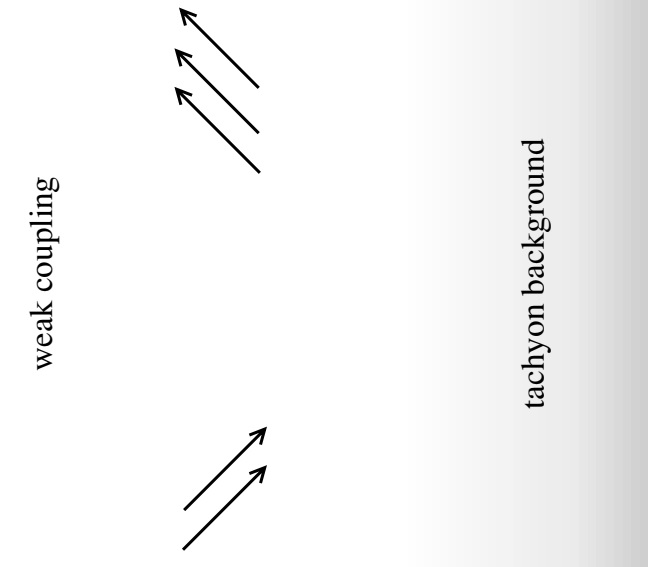
\includegraphics[width=0.8\textwidth]{figure/Fig9.12.jpg}\\
		\caption{Spacetime with dilaton and tachyon in the background. The further to the right, the stronger the interaction, but it is cut off by an effective potential from the tachyon background.}\label{Fig9.12}
	\end{center}
\end{figure}
\vspace*{-0.7cm}

When $D>2$, although it has been argued that the tachyon background acts like a potential barrier, its physical effect is not very clear. 
However, there is another reason to focus on $D \leq 2$: these theories are actually solvable.
Let's first observe that when we quantize the string, gauge symmetry will take away two families of oscillators. 
This leaves nothing when $D \leq 2$—only the center of mass motion, a scalar.\footnote{For some special momenta, extra physical states are found. They can be interpreted as unbroken symmetries of string field theory and may play a role in the solvability of the theory.} However, directly solving this string theory is quite difficult. First, the world-sheet path integral with the action \eqref{9.9.5} must be calculated. 
Due to the exponential tachyon field, this is no longer a free theory. It is called Liouville field theory.
It is classically integrable, and after some effort, some quantum amplitudes can be determined. 
However, to solve string theory, we need to integrate this result over every genus in the Riemann surface moduli space; we have seen that this is a compact space. 
Quite remarkably, amplitudes up to all orders have been determined through a quite different method. To describe this method, we must first introduce another concept.

\subsection*{Non-critical strings}

Consider a statistical mechanics system defined by summing over two-dimensional surfaces in $d$-dimensional Euclidean space. We also assume that the surfaces have some internal degrees of freedom that can be interpreted as a measure of length.
The natural fields to describe this system are the embedding $X^{\mu}(\sigma)$ and the metric $g_{a b}(\sigma)$. However, there is no reason to throw the length out of this problem—that is, the theory is not necessarily Weyl invariant. 
Thus it is called a non-critical string. The lowest dimensional action for this system is the Polyakov action with an extra world-sheet constant term, such as would be prohibited by Weyl invariance in critical strings:
\begin{equation}
	S=\frac{1}{4 \pi \alpha^{\prime}} \int_{M} \dif^{2} \sigma \: g^{1/2} 
	\Bigl(g^{ab} \partial_{a} X^{\mu} \partial_{b} X_{\mu}+\mu\Bigr) \:.
	\label{9.9.6}
\end{equation}

Without Weyl invariance, we can partially determine the metric with diff-invariance, but one degree of freedom will remain:
\begin{equation}
	g_{ab}(\sigma)=\exp (2 \phi(\sigma)) \hat{g}_{ab}(\sigma) \:, \label{9.9.7}
\end{equation}
where $\hat{g}_{ab}$ is a gauge choice, and the metric scale $\phi$ still needs to be integrated in the path integral. A gauge-fixed Faddeev-Popov determinant is the same as \eqref{3.4.19}, 
and the contribution of Weyl fixing to the latter is trivial.
Substituting the metric \eqref{9.9.7}, the curvature is:
\begin{equation}
	g^{1/2} R = \hat{g}^{1/2}\Bigl(\hat{R}-2 \hat{\nabla}^{2} \phi\Bigr) \:, \label{9.9.8}
\end{equation}
\begin{tcolorbox}[breakable]
	\begin{remark}
		Locally write $\hat g_{ab}=\me^{2\hat\omega}\delta_{ab}$. In two dimensions $R[\me^{2\omega}\delta]=-2\me^{-2\omega}\partial^2\omega$ with $\partial^2$ the flat Laplacian, and $\hat\nabla^2=\me^{-2\hat\omega}\partial^2$ on scalars. Then
		\begin{equation*}
			g^{1/2}R\eqs{1}\me^{2\phi+2\hat\omega}\cdot\bigl(-2\me^{-2\phi-2\hat\omega}\partial^2(\phi+\hat\omega)\bigr)=-2\partial^2\hat\omega-2\partial^2\phi\eqs{2}\hat g^{1/2}\bigl(\hat R-2\hat\nabla^2\phi\bigr).
		\end{equation*}
		At (1) $g=\me^{2(\phi+\hat\omega)}\delta$. At (2) $-2\partial^2\hat\omega=\hat g^{1/2}\hat R$ and $\partial^2\phi=\me^{2\hat\omega}\hat\nabla^2\phi=\hat g^{1/2}\hat\nabla^2\phi$. Both sides are covariant, so the local result holds globally. In particular $\int g^{1/2}R$ is independent of $\phi$, which is Gauss--Bonnet.
	\end{remark}
\end{tcolorbox}
throwing away field-independent terms, this action plus the Faddeev-Popov determinant becomes:
\begin{equation}
	S=\frac{1}{4 \pi \alpha^{\prime}} \int_{M} \dif^{2} \sigma \: \hat{g}^{1/2} \biggl[\hat{g}^{ab} \partial_{a} X^{\mu} \partial_{b} X_{\mu}+\mu \exp 2 \phi + \frac{13 \alpha^{\prime}}{3}\Bigl(\hat{g}^{ab} \partial_{a} \phi \partial_{b} \phi+\hat{R} \phi\Bigr)\biggr]\:.
	\label{9.9.9}
\end{equation}
Note that the Faddeev-Popov determinant provides a kinetic energy term for $\phi$.
\begin{tcolorbox}[breakable]
	\begin{remark}
		Conventions (Section \ref{sec:3.4}). For a CFT of central charge $c$, $\delta_{\mathrm W}\ln Z=-\frac{1}{2\pi}\int\dif^2\sigma\,g^{1/2}\delta\omega\,T^a{}_a$ with $T^a{}_a=-\frac{c}{12}R$. As in the text, the $X^\mu$ path integral is still defined with the full metric $g$. Only the ghost determinant is rewritten in terms of $\hat g$, so the relevant central charge is $c^{\mathrm g}=-26$.

		\emph{Integrated anomaly.} Along the path $g_s=\me^{2s\phi}\hat g$, $0\le s\le1$, we have $\delta\omega=\phi\,\dif s$ and $g_s^{1/2}R_s=\hat g^{1/2}(\hat R-2s\hat\nabla^2\phi)$ by \eqref{9.9.8}. Then
		\begin{align*}
			\ln\frac{Z[\me^{2\phi}\hat g]}{Z[\hat g]}&\eqs{1}\frac{c}{24\pi}\int_0^1\dif s\int\dif^2\sigma\,\hat g^{1/2}\phi\bigl(\hat R-2s\hat\nabla^2\phi\bigr)
			=\frac{c}{24\pi}\int\dif^2\sigma\,\hat g^{1/2}\bigl(\phi\hat R-\phi\hat\nabla^2\phi\bigr)\\
			&\eqs{2}\frac{c}{24\pi}\int\dif^2\sigma\,\hat g^{1/2}\bigl(\hat g^{ab}\partial_a\phi\partial_b\phi+\hat R\phi\bigr) .
		\end{align*}
		At (1) $\delta_{\mathrm W}\ln Z=\frac{c}{24\pi}\int g^{1/2}R\,\delta\omega$. At (2) the $\phi\hat\nabla^2\phi$ term was integrated by parts.

		\emph{Coefficient in \eqref{9.9.9}.} For the ghosts $c=-26$, so the determinant contributes $\me^{-S_\phi}$ with
		\begin{equation*}
			S_\phi=\frac{26}{24\pi}\int\hat g^{1/2}\bigl(\hat g^{ab}\partial_a\phi\partial_b\phi+\hat R\phi\bigr)=\frac{1}{4\pi\alpha'}\cdot\frac{13\alpha'}{3}\int\hat g^{1/2}\bigl(\hat g^{ab}\partial_a\phi\partial_b\phi+\hat R\phi\bigr),
		\end{equation*}
		since $\frac{26}{24\pi}=\frac{13}{12\pi}=\frac{1}{4\pi\alpha'}\cdot\frac{13\alpha'}{3}$. The cosmological term is $\mu g^{1/2}=\mu\,\me^{2\phi}\hat g^{1/2}$, and $g^{1/2}g^{ab}$ is Weyl invariant, so the $X$ kinetic term keeps its form. This reproduces \eqref{9.9.9}.

		If the $X^\mu$ measure were also converted to $\hat g$, their $c=d$ would change $26\to26-d$. Making $\phi$ itself a free field with measure defined by $\hat g$ adds its own $c=1$. These are the ``somewhat different coefficients'' mentioned in the text. Once they are included, $\phi$ becomes the linear dilaton direction $X^1$ with $D=d+1$: $V_1^2=(26-D)/6\alpha'$ matches $(25-d)/6\alpha'$ (the Distler--Kawai--David result, quoted here, not derived).
	\end{remark}
\end{tcolorbox} Compared with the dilaton-tachyon action \eqref{9.9.5}, we see a remarkable similarity. 
If we set $d=D-1$ and interpret the new field $\phi$ as $x^{1}$, and rename $g_{a b} \to \hat{g}_{a b}$ in action \eqref{9.9.5}, then the same terms appear. 
Some coefficients will be somewhat different—there is no rescaling of $\phi$ that makes them all consistent—but in fact, we claim they are the same field theory.
The key is that the critical string path integral \eqref{9.9.5} is defined using $\hat{g}_{ab}$ as the metric, while non-critical strings \eqref{9.9.9} use $\exp (2 \phi) \hat{g}_{a b}$. 
A careful treatment of the Weyl transformation of the measure can convert one to the other.
To understand this, note that only the total metric \eqref{9.9.7} appears in the definition of critical strings, so in the transformation:
\begin{subequations} \label{9.9.10}
	\begin{align}
		\hat{g}_{a b}(\sigma)  &\rightarrow \exp (2 \omega(\sigma)) \hat{g}_{a b}(\sigma) \:,  \label{9.9.10a}\\
		\phi(\sigma) &\rightarrow \phi(\sigma)-\omega(\sigma) \:, \label{9.9.10b}
	\end{align}
\end{subequations}
all quantities are invariant.
Thus non-critical strings gain Weyl invariance, which is sufficient to fix various coefficients other than the free parameter $\mu$.

A Weyl-invariant theory and a non-Weyl-invariant theory can be equivalent, which seems strange. The key is that in field theory, if we simultaneously increase the fields used only to fix the gauge, we can always add extra ``fake'' gauge symmetry. 
After all, a gauge symmetry is just a redundant description, and we can always adopt a more redundant description. For the symmetry \eqref{9.9.10}, we can obviously just cancel the Weyl symmetry of field $\phi$. 
But for general string backgrounds (for example, flat space, where the embedding coordinates are Weyl invariant), this is impossible, and Weyl invariance is ``real.''
In any case, we have now reached a very subtle situation where we can approximate non-critical strings by summing over triangulated surfaces, where the number of edges between two points becomes a measure of length. 
These triangulated surfaces are similar to large Feynman diagrams, and in fact we can find a quantum system—matrix model, which is a diagrammatic expansion. 
The fields of the matrix model are $N \times N$ matrices. Taking $N \rightarrow \infty$ and adjusting other couplings, (at least for $D \leq 2$) there exists a critical point dominated by smooth large surfaces, 
so we recover non-critical strings.
Furthermore, by diagonalizing the matrix (at least for $D \leq 2$), the matrix model is solvable. 
At the end, we obtain a quite simple system (non-interacting fermions moving in the eigenvalue space), and reversing the above steps allows for the calculation of string amplitudes to any order.

We leave the details to the references. In any case, when $D>2$ or in supersymmetric theories, they have not yet been found to be useful. 
However, at least we mention an important lesson learned from these models. The $(2g)!$ behavior in perturbation theory was originally seen in explicit matrix models, and from this, it was argued that it holds for all string theories.
In matrix models, the corresponding $\exp [O(-1 / g_{\mathrm{c}})]$ effects include tunneling of fermions in the eigenvalue space. 
Whether this is related to $\exp [O(-1 / g_{\mathrm{c}})]$ effects in higher dimensional string theories is still unclear.
	\setcounter{section}{0}% Change the value of the chapter counter
%\numberwithin{equation}{chapter}% Equation counter subordinated to the section counter
\numberwithin{equation}{section}% Equation counter subordinated to the section counter
\numberwithin{figure}{section}% Figure counter subordinated to the section counter
\setcounter{chapter}{9}
\chapter{\texorpdfstring{Type I and Type II Superstrings}{10 Type I and Type II Superstrings}} \label{cha:10}


\section{Superconformal Algebra}

In the bosonic string, the mass-shell condition
\begin{equation}
	p_{\mu}p^{\mu}+m^{2}=0 \label{10.1.1}
\end{equation}
comes from the physical state condition
\begin{equation}
	L_{0}\lvert \psi\rangle = 0\: , \label{10.1.2}
\end{equation}
and in the closed string, $\tilde{L}_{0}\lvert\psi\rangle=0$ must also be added. To obtain fermions, we need the Dirac equation
\begin{equation}
	\mi p_{\mu} \Gamma^{\mu}+m=0\:. \label{10.1.3}
\end{equation}

In the bosonic string, $L_{0}$ and $\tilde{L}_{0}$ are the center-of-mass modes of the energy-momentum tensor $(T_{B},\tilde{T}_{B})$. Now we want to introduce new conserved quantities $T_{F}$ and $\tilde{T}_{F}$, such that their center-of-mass modes yield the Dirac equation. Note that since the spacetime momentum $p^{\mu}$ is the center-of-mass mode of the worldsheet currents $(\partial X^{\mu},\bar{\partial}X^{\mu})$, we now expect the $\Gamma$ matrices satisfying the algebra
\begin{equation}
	\{\Gamma^{\mu},\Gamma^{\nu}\}=2\eta^{\mu\nu} \:, \label{10.1.4}
\end{equation}
to be the center-of-mass modes of the anticommuting worldsheet fields $\psi^{\mu}$.

Now let us examine the worldsheet action
\begin{equation}
	S=\frac{1}{4\uppi}\int\dif^{2}z \:
	\left(
	\frac{2}{\alpha^{\prime}}\partial X^{\mu}\bar{\partial}X_{\mu} +\psi^{\mu}\bar{\partial}\psi_{\mu}
	+\tilde{\psi}^{\mu}\partial\tilde{\psi}_{\mu}
	\right)\:.\label{10.1.5}
\end{equation}
The OPE of $XX$ is
\begin{equation}
	X^{\mu}(z,\bar{z})X^{\nu}(0,0)\sim -\frac{\alpha^{\prime}}{2}\eta^{\mu\nu}\ln\lvert z\rvert^{2}\:.\label{10.1.6}
\end{equation}
$\psi$ and $\tilde{\psi}$ are holomorphic and antiholomorphic, respectively, and their OPEs are
\begin{equation}
	\psi^{\mu}(z)\psi^{\nu}(0)\sim\frac{\eta^{\mu\nu}}{z}\:,\qquad
	\tilde{\psi}^{\mu}(\bar{z})\tilde{\psi}^{\nu}(0)\sim\frac{\eta^{\mu\nu}}{\bar{z}}\: \label{10.1.7}
\end{equation}
The \emph{worldsheet supercurrents} are
\begin{equation}
	T_{F}(z)=\mi(2/\alpha^{\prime})^{1/2}\psi^{\mu}(z)\partial X_{\mu}(z)\:,\qquad
	\tilde{T}_{F}(\bar{z})=\mi(2/\alpha^{\prime})^{1/2}\tilde{\psi}^{\mu}(\bar{z})\bar{\partial} X_{\mu}(\bar{z})
	\:.\label{10.1.8}
\end{equation}
\begin{tcolorbox}[breakable]
\begin{proof}
		We consider the left-moving part of the action
		\begin{equation}
			S_L=\frac{1}{4\pi}\int d^2z\left(\frac{2}{\alpha'}\partial X^\mu \bar\partial X_\mu+\psi^\mu\bar\partial\psi_\mu\right).
		\end{equation}
		
		We take a local supersymmetry transformation with parameter $\epsilon(z,\bar z)$:
		\begin{align}
			\delta X^\mu &= \epsilon(z,\bar z)\,\psi^\mu, \\
			\delta \psi^\mu &= -\frac{2}{\alpha'}\,\epsilon(z,\bar z)\,\partial X^\mu.
		\end{align}

		Because the grassmann variables anti-commute, we have
		\begin{equation}
			\delta\!\left(\int \psi^\mu \bar\partial \psi_\mu\right)
			= 2 \int \delta\psi^\mu\,\bar\partial \psi_\mu,
		\end{equation}
		up to boundary terms. Hence
		\begin{align}
			\delta S_\psi
			&= \frac{1}{2\pi}\int d^2z\, \delta\psi^\mu\,\bar\partial \psi_\mu= -\frac{1}{2\pi\alpha'}\int d^2z\, 2\mathcolor{red}{\epsilon\,\partial X^\mu\,\bar\partial \psi_\mu}.
		\end{align}
		The bosonic part can be given as:
		\begin{align}
			\delta S_X
			&= \frac{1}{4\pi}\int d^2z\,\frac{2}{\alpha'}
			\left(\partial(\epsilon\psi^\mu)\bar\partial X_\mu + \partial X^\mu \bar\partial(\epsilon\psi_\mu)\right).
		\end{align}
		Using
		\begin{align}
			\partial(\epsilon\psi^\mu) &= (\partial \epsilon)\psi^\mu + \epsilon\,\partial \psi^\mu, \\
			\bar\partial(\epsilon\psi^\mu) &= (\bar\partial \epsilon)\psi^\mu + \epsilon\,\bar\partial \psi^\mu.
		\end{align}
		We have:
		\begin{align}
			\delta S_X
			= \frac{1}{2\pi\alpha'}\int d^2z \Big[
			(\partial\epsilon)\psi^\mu\bar\partial X_\mu
			+ \epsilon\,\partial\psi^\mu\bar\partial X_\mu + (\bar\partial\epsilon)\psi^\mu\partial X_\mu
			+\mathcolor{red}{ \epsilon\,\partial X^\mu\bar\partial\psi_\mu}
			\Big].
		\end{align}
		Adding $\delta S_X$ and $\delta S_\psi$:
		\begin{align}
			\delta S
			= \frac{1}{2\pi\alpha'}\int d^2z \Big[
			(\partial\epsilon)\psi^\mu\bar\partial X_\mu
			+ (\bar\partial\epsilon)\psi^\mu\partial X_\mu  + \epsilon\big(\partial\psi^\mu\bar\partial X_\mu - \partial X^\mu\bar\partial\psi_\mu\big)
			\Big].
		\end{align}
		From Integration by parts, we have:
		
		\begin{align}
			\int (\partial\epsilon)\psi^\mu\bar\partial X_\mu
			&= -\int \epsilon\,\partial(\psi^\mu\bar\partial X_\mu) \\
			&= -\int \epsilon\big(\partial\psi^\mu\bar\partial X_\mu + \psi^\mu \partial\bar\partial X_\mu\big).
		\end{align}
		
		Using $\partial\bar\partial X_\mu = \bar\partial\partial X_\mu$, and dropping the total derivative-terms. We are left with
		\begin{align*}
			\delta S
			&= \frac{1}{2\pi\alpha'}\int d^2z \Big[
			-\cancel{\epsilon\partial\psi^\mu\bar\partial X_\mu} + \bar\partial\epsilon\psi^\mu \partial X_\mu+\cancel{\epsilon\partial X^\mu\bar\partial\psi_\mu}
			+ (\bar\partial\epsilon)\psi^\mu\partial X_\mu \\
			&\qquad + \epsilon\big(\cancel{\partial\psi^\mu\bar\partial X_\mu} - \cancel{\partial X^\mu\bar\partial\psi_\mu}\big)
			\Big]\\
			&= \frac{1}{2\pi}\int d^2z\,(\bar\partial \epsilon)\left(\frac{2}{\alpha'}\,\psi^\mu \partial X_\mu\right).
		\end{align*}
		Thus the holomorphic supercurrent is
		\begin{equation}
			\boxed{
				G(z)=\frac{2}{\alpha'}\,\psi^\mu \partial X_\mu
			}
		\end{equation}
		
		and similarly for right moving part:
		\begin{equation}
			\boxed{
				\tilde G(\bar z)=\frac{2}{\alpha'}\,\tilde\psi^\mu \bar\partial X_\mu
			}
		\end{equation}
\end{proof}
\end{tcolorbox}
This gives the desired result: the $\psi_{0}^{\mu}$ and $\tilde{\psi}_{0}^{\mu}$ modes will satisfy the Gamma matrix algebra, and the center-of-mass modes of $T_{F}$ and $\tilde{T}_{F}$ take the form of the Dirac operator. 

From the OPE and Ward identities, it can be concluded that the currents
\begin{equation}
	j^{\eta}(z)=\eta(z)T_{F}(z)\:, \qquad
	\tilde{\jmath}(\bar{z})=\bar{\eta}(\bar{z}) \tilde{T}_{F}(\bar{z}) \label{10.1.9}
\end{equation}
generate \emph{superconformal transformations}
\begin{subequations}
	\begin{align}
		\epsilon^{-1}(2/\alpha^{\prime})^{1/2}\delta X^{\mu}(z,\bar{z}) &= \eta(z)\psi^{\mu}(z) + \eta(z)^{\ast} \tilde{\psi}^{\mu}(\bar{z})\:, \label{10.1.10a} \\
		\epsilon^{-1}(2/\alpha^{\prime})^{1/2}\delta \psi^{\mu}(z) &= -\eta(z)\partial X^{\mu}(z) \:, \label{10.1.10b}  \\
		\epsilon^{-1}(2/\alpha^{\prime})^{1/2}\delta\tilde{\psi}^{\mu}(\bar{z}) &=-\eta(z)^{\ast}\bar{\partial} X^{\mu}(\bar{z}) \:. \label{10.1.10c}
	\end{align}
\end{subequations}
This transformation mixes the commuting field $X^{\mu}$ and the anticommuting fields $\psi^{\mu}$ and $\tilde{\psi}^{\mu}$, so $\eta(z)$ must be an anticommuting parameter. 

\begin{tcolorbox}[breakable]
	\noindent We now examine the OPE of $T_{F},\tilde{T}_{F}$ with $X,\psi ,\tilde{\psi}$: \\
	(1)
	\begin{align*}
		T_{F}(w)X^{\mu }(z,\bar{z}) &=\mi(2/\alpha ^{\prime })^{1/2}\psi ^{\nu
		}(w)\partial X_{\nu }(w)X^{\mu }(z,\bar{z}) \\
		&=\mi(2/\alpha ^{\prime })^{1/2}\psi ^{\nu }(w)\partial _{w}\delta _{\nu
		}^{\mu }\left( -\frac{\alpha ^{\prime }}{2}\ln \lvert z-w\rvert
		^{2}\right)  \\
		&=-\mi\left( \alpha ^{\prime }/2\right) ^{1/2}\frac{\psi ^{\mu }(w)}{w-z}
	\end{align*}%
	Similarly, we can obtain \[
	\tilde{T}_{F}(\bar{w})X^{\mu }(z,\bar{z})=-\mi\left( \alpha ^{\prime
	}/2\right) ^{1/2}\frac{\tilde{\psi}^{\mu }(\bar{w})}{\bar{w}-\bar{z}}
	\]%
	Using the Ward identity \[
	\frac{1}{\mi\epsilon }\delta \mathscr{A}(z,\bar{z})=\operatorname{Res}_{w\rightarrow z}j(w)\mathscr{A}(z,%
	\bar{z})+\overline{\operatorname{Res}}_{\bar{w}\rightarrow \bar{z}}\tilde{\jmath}(\bar{w})\mathscr{A}(z,\bar{z}%
	)
	\]%
	we get \begin{align*}
		\frac{1}{\mi\epsilon }\delta X(z,\bar{z}) &=\eta (z)\left( -\mi\left( \alpha
		^{\prime }/2\right) ^{1/2}\psi ^{\mu }(z)\right) +\eta (z)^{\ast }\left(
		-\mi\left( \alpha ^{\prime }/2\right) ^{1/2}\tilde{\psi}^{\mu }(\bar{z}%
		)\right)  \\
		\epsilon ^{-1}\left( 2/\alpha ^{\prime }\right) ^{1/2}\delta X(z,\bar{z})
		&=\eta (z)\psi ^{\mu }(z)+\eta (z)^{\ast }\tilde{\psi}^{\mu }(\bar{z})
	\end{align*}%
	(2) %
	\begin{align*}
		T_{F}(w)\psi ^{\mu }(z) &=\mi(2/\alpha ^{\prime })^{1/2}\psi ^{\nu
		}(w)\partial X_{\nu }(w)\psi ^{\mu }(z) \\
		&=\mi(2/\alpha ^{\prime })^{1/2}\frac{\eta ^{\mu \nu }}{w-z}\partial X_{\nu
		}(w) \\
		&=\mi(2/\alpha ^{\prime })^{1/2}\frac{\partial X^{\mu }(w)}{w-z}
	\end{align*}%
	Using the Ward identity, we obtain \begin{align*}
		\frac{1}{i\epsilon }\delta \psi ^{\mu }(z) &=\eta (z)\left( \mi(2/\alpha
		^{\prime })^{1/2}\partial X^{\mu }(z)\right)  \\
		\epsilon ^{-1}(\alpha ^{\prime }/2)^{1/2}\delta \psi ^{\mu }(z) &=-\eta
		(z)\partial X^{\mu }(z)
	\end{align*}%
	(3) Similarly, we obtain (\ref{10.1.10c})
\end{tcolorbox}

The commutator of two superconformal transformations is a conformal transformation,
\begin{equation}
	\delta_{\eta_{1}}\delta_{\eta_{2}}-\delta_{\eta_{2}}\delta_{\eta_{1}}=\delta_{v}\:,\qquad
	v(z)= -2\eta_{1}(z)\eta_{2}(z) \:, \label{10.1.11}
\end{equation}
similarly, the commutator of a conformal transformation and a superconformal transformation is a superconformal transformation.
\begin{tcolorbox}[breakable]
	First, verify (\ref{10.1.11}) for $X$:
	\begin{align*}
		\delta_{\eta_{1}}\delta_{\eta_{2}}X &=  (\alpha^{\prime}/2)^{1/2}
		\delta_{\eta_{1}}(\eta_{2}(z)\psi^{\mu}(z) + \eta_{2}(z)^{\ast} \tilde{\psi}^{\mu}(\bar{z})) \\
		&=-(\alpha^{\prime}/2)^{1/2} (2/\alpha^{\prime})^{1/2}
		(\eta_{2}(z)\eta_{1}(z)\partial X^{\mu}(z) + \eta_{2}(z)^{\ast} \eta_{1}(z)^{\ast}\bar{\partial}X^{\mu}(\bar{z}))  \\
		&=
		\eta_{1}(z)\eta_{2}(z)\partial X^{\mu}(z) +
		\eta_{1}(z)^{\ast} \eta_{2}(z)^{\ast}\bar{\partial}X^{\mu}(\bar{z})
	\end{align*}
	Therefore,
	\begin{equation*}
		[\delta_{\eta_{1}},\delta_{\eta_{2}}]X= 
		2\eta_{1}\eta_{2}\partial X^{\mu} + 2\eta_{1}^{\ast} \eta_{2}^{\ast}\bar{\partial}X^{\mu}
		=\delta_{v}X
	\end{equation*}
	See \eqref{2.4.7}.
	
	Next, verify (\ref{10.1.11}) for $\psi$:
	\begin{align*}
		\delta _{\eta _{1}}\delta _{\eta _{2}}\psi ^{\mu } &=-\delta _{\eta
			_{1}}\left( \eta _{2}(z)\partial X^{\mu }(z)\right) =-\eta _{2}(z)\partial
		(\delta _{\eta _{1}}X^{\mu }(z)) \\
		&=-\eta _{2}(z)\partial (\eta _{1}(z)\psi ^{\mu }(z)+\eta _{1}(z)^{\ast }%
		\tilde{\psi}^{\mu }(\bar{z})) \\
		&=-\eta _{2}\eta _{1}\partial \psi ^{\mu }-\eta _{2}(\partial \eta
		_{1})\psi ^{\mu }
	\end{align*}%
	So \begin{align*}
		\lbrack \delta _{\eta _{1}},\delta _{\eta _{2}}]\psi ^{\mu } &=-\eta
		_{2}\eta _{1}\partial \psi ^{\mu }-\eta _{2}(\partial \eta _{1})\psi ^{\mu
		}+\eta _{1}\eta _{2}\partial \psi ^{\mu }+\eta _{1}(\partial \eta _{2})\psi
		^{\mu } \\
		&=2\eta _{1}\eta _{2}\partial \psi ^{\mu }+\partial (\eta _{1}\eta
		_{2})\psi ^{\mu }
	\end{align*}%
	Since $\psi$ is a $(\frac{1}{2},0)$ field, this is exactly $\delta _{v}\psi $. In fact, for a primary field $\mathcal{O}$ with weight $(h,0)$, according to \eqref{2.4.16} \[
	T(z)\mathcal{O}(w,\bar{w})=\frac{h}{(z-w)^{2}}\mathcal{O}(w,\bar{w})+\frac{1}{(z-w)}\partial \mathcal{O}(w,%
	\bar{w})+\cdots \text{ ,}
	\]%
	the Ward identity gives \begin{align*}
		\frac{1}{\mi }\delta _{v}\mathcal{O} &=\operatorname{Res}_{z\to w}\Bigl(\mi v(z)T(z)\mathcal{O}(w,%
		\bar{w})\Bigr) \\
		\delta _{v}\mathcal{O} &=-\left( h(\partial v)\mathcal{O}+v\partial \mathcal{O}\right)
	\end{align*}
	It is similar for $\tilde{\psi}$.
	
	Now let's examine the commutator of conformal transformations and superconformal transformations, first for $X$:
	\begin{align*}
		\delta _{\eta }\delta _{v}X &=\delta _{\eta }(-v\partial X-v^{\ast }\bar{%
			\partial}X)=-v\partial \left( \delta _{\eta }X\right) -v^{\ast }\bar{\partial%
		}\left( \delta _{\eta }X\right)  \\
		&=-v\partial \left( \eta \psi +\eta ^{\ast }\tilde{\psi}\right) -v^{\ast }%
		\bar{\partial}\left( \eta \psi +\eta ^{\ast }\tilde{\psi}\right)  \\
		&=-v(\partial \eta )\psi -v\eta \partial \psi -v^{\ast }(\partial \eta
		)^{\ast }\tilde{\psi}-v^{\ast }\eta ^{\ast }\bar{\partial}\tilde{\psi}
	\end{align*}%
	while
	\begin{align*}
		\delta _{v}\delta _{\eta }X &=\delta _{v}(\eta \psi +\eta ^{\ast }\tilde{%
			\psi})=\eta \left( -v\partial \psi -\tfrac{1}{2}\left( \partial v\right) \psi
		\right) +\eta ^{\ast }\left( -v^{\ast }\bar{\partial}\tilde{\psi}-\tfrac{1}{2}%
		\left( \partial v\right) ^{\ast }\tilde{\psi}\right)
	\end{align*}%
	so
	\begin{align*}
		\lbrack \delta _{\eta },\delta _{v}]X &=-v(\partial \eta )\psi -v\eta
		\partial \psi -v^{\ast }(\partial \eta )^{\ast }\tilde{\psi}-v^{\ast }\eta
		^{\ast }\bar{\partial}\tilde{\psi} \\
		&\quad+\eta v\partial \psi +\tfrac{1}{2}\eta \left( \partial v\right) \psi +\eta
		^{\ast }v^{\ast }\bar{\partial}\tilde{\psi}+\tfrac{1}{2}\eta ^{\ast }\left(
		\partial v\right) ^{\ast }\tilde{\psi} \\
		&=-v(\partial \eta )\psi -v^{\ast }(\partial \eta )^{\ast }\tilde{\psi}+%
		\tfrac{1}{2}\eta \left( \partial v\right) \psi +\tfrac{1}{2}\eta ^{\ast
		}\left( \partial v\right) ^{\ast }\tilde{\psi} \\
		&=\delta _{\eta ^{\prime }}X
	\end{align*}%
	where \[
	\eta ^{\prime }=-v\partial \eta +\tfrac{1}{2}\eta \partial v
	\]%
	For $\psi$:
	\begin{align*}
		\delta _{\eta }\delta _{v} \psi  &=\delta _{\eta }\left( -v\partial \psi +%
		\tfrac{1}{2}(\partial v)\psi \right) =-v\partial \left( \delta _{\eta }\psi
		\right) +\tfrac{1}{2}(\partial v)\delta _{\eta }\psi  \\
		&=-v\partial \left( \eta \partial X\right) -\frac{1}{2}(\partial v)\eta
		\partial X \\
		&=-v\eta \partial ^{2}X-v\partial \eta \partial X-\tfrac{1}{2}(\partial
		v)\eta \partial X
	\end{align*}%
	while \begin{align*}
		\delta _{v}\delta _{\eta }\psi  &=\delta _{v}(\eta \partial X)=\eta
		\partial (\delta _{v}X)=\eta \partial (-v\partial X-v^{\ast }\bar{\partial}X)
		\\
		&=-\eta \partial v\partial X-\eta v\partial ^{2}X
	\end{align*}%
	so \begin{align*}
		\lbrack \delta _{\eta },\delta _{v}]\psi  &=-v\eta \partial ^{2}X-v\partial
		\eta \partial X-\tfrac{1}{2}(\partial v)\eta \partial X+\eta \partial
		v\partial X+\eta v\partial ^{2}X \\
		&=-v\partial \eta \partial X+\tfrac{1}{2}(\partial v)\eta \partial X \\
		&=\delta _{\eta ^{\prime }}X
	\end{align*}%
	It is similar for $\tilde{\psi}$.
\end{tcolorbox}
From the above, we see that conformal transformations and superconformal transformations are closed; together they form the \emph{superconformal algebra}. In terms of currents, this means that the OPE of $T_{F}$ and $T_{B}$ is closed, but at this point $T_{B}$ must include the fermion part
\begin{equation}
	T_{B}=-\frac{1}{\alpha^{\prime}}\partial X^{\mu}\partial X_{\mu}-\frac{1}{2}\psi^{\mu}\partial\psi_{\mu}
\end{equation}
\begin{tcolorbox}[breakable]
	\begin{proof}
			We start from
		\begin{equation}
			S=\frac{1}{4\pi}\int d^2z\left(\frac{2}{\alpha'}\partial X^\mu \bar\partial X_\mu+\psi^\mu\bar\partial\psi_\mu+\tilde\psi^\mu\partial\tilde\psi_\mu\right).
		\end{equation}
		For the Holomorphic part of $T(z)$, we consider the following variation
		\begin{align}
			\delta X^\mu &= -\zeta(z)\,\partial X^\mu, \\
			\delta \psi^\mu &= -\zeta(z)\,\partial \psi^\mu - \frac{1}{2}(\partial \zeta(z))\psi^\mu, \\
			\delta \tilde{\psi}^\mu &= 0.
		\end{align}
		Let us look at bosonic part of the action first
	%	\begin{equation}
	%		S_X = \frac{1}{4\pi} \int d^2z\,\frac{2}{\alpha'} \partial X^\mu \bar\partial X_\mu.
	%	\end{equation}
		
		\begin{align}
			\delta S_X &= \frac{1}{4\pi} \int d^2z\,\frac{2}{\alpha'} 
			\left(\partial(\delta X^\mu)\bar\partial X_\mu + \partial X^\mu \bar\partial(\delta X_\mu)\right).
		\end{align}
		
		Inserting $\delta X^\mu = -\zeta \partial X^\mu$:
		\begin{align}
			\partial(\delta X^\mu) &= -(\partial \zeta)\partial X^\mu - \zeta \partial^2 X^\mu, \\
			\bar\partial(\delta X^\mu) &= -(\bar\partial \zeta)\partial X^\mu - \zeta \bar\partial \partial X^\mu.
		\end{align}
		The bosonic part of the variation takes the following form:
		\begin{align}
			\delta S_X &= \frac{1}{2\pi \alpha'} \int d^2z \Big[
			-(\partial \zeta)\partial X^\mu \bar\partial X_\mu
			- \mathcolor{red}{\zeta \partial^2 X^\mu \bar\partial X_\mu}  - (\bar\partial \zeta)\partial X^\mu \partial X_\mu
			- \mathcolor{red}{\zeta \partial X^\mu \bar\partial \partial X_\mu}
			\Big]\notag\\
		&= \frac{1}{2\pi \alpha'} \int d^2z \Big[
			-(\partial \zeta)\partial X^\mu \bar\partial X_\mu
			  - (\bar\partial \zeta)\partial X^\mu \partial X_\mu
			-\mathcolor{red}{\zeta \partial(\partial X^\mu \bar\partial X_\mu)}
			\Big]\notag\\
			&= -\frac{1}{2\pi \alpha'} \int d^2z\, (\bar\partial \zeta)\, \partial X^\mu \partial X_\mu.
		\end{align}
		Similarly, we can find the variation of fermionic part as follows:
		
		%\begin{equation}
		%	S_\psi = \frac{1}{4\pi} \int d^2z\, \psi^\mu \bar\partial \psi_\mu.
		%\end{equation}
		
		\begin{align}
			\delta S_\psi &= \frac{1}{4\pi} \int d^2z \left(
			\delta \psi^\mu \bar\partial \psi_\mu + \psi^\mu \bar\partial(\delta \psi_\mu)
			\right).
		\end{align}
		
		Inserting
		\begin{equation}
			\delta \psi^\mu = -\zeta \partial \psi^\mu - \frac{1}{2}(\partial \zeta)\psi^\mu.
		\end{equation}
		Then,
		\begin{align}
			\delta S_\psi &= \frac{1}{4\pi} \int d^2z \Big[
			-\zeta \partial \psi^\mu \bar\partial \psi_\mu
			-\frac{1}{2}(\partial \zeta)\psi^\mu \bar\partial \psi_\mu - \psi^\mu \bar\partial(\zeta \partial \psi_\mu)
			-\frac{1}{2}\psi^\mu \bar\partial((\partial \zeta)\psi_\mu)
			\Big].
		\end{align}
		It can be simplified using:
		\begin{align}
			\psi^\mu \bar\partial(\zeta \partial \psi_\mu)
			&= (\bar\partial \zeta)\psi^\mu \partial \psi_\mu
			+ \zeta \psi^\mu \bar\partial \partial \psi_\mu,\\
			\psi^\mu \bar\partial((\partial \zeta)\psi_\mu)
			&= (\bar\partial\partial \zeta)\underbrace{\psi^\mu  \psi_\mu}_{=0}+(\partial \zeta)\psi^\mu \bar\partial \psi_\mu.
		\end{align}
		Thus,
		\begin{align}
			\delta S_\psi &=\frac{1}{4\pi} \int d^2z \Big[
			-\zeta \partial \psi^\mu \bar\partial \psi_\mu
			-\frac{1}{2}(\partial \zeta)\psi^\mu \bar\partial \psi_\mu -(\bar\partial \zeta)\psi^\mu \partial \psi_\mu- \zeta \psi^\mu \bar\partial \partial \psi_\mu
			-\frac{1}{2}(\partial \zeta)\psi^\mu \bar\partial \psi_\mu
			\Big]\notag\\ 
			&=\frac{1}{4\pi} \int d^2z \Big[
			-\zeta\underbrace{(\partial \psi^\mu \bar\partial \psi_\mu + \psi^\mu \bar\partial \partial \psi_\mu)}_{\partial(\psi^\mu \bar\partial \psi_\mu)}-(\bar\partial \zeta)\psi^\mu \partial \psi_\mu
			- (\partial \zeta)\psi^\mu \bar\partial \psi_\mu
			\Big]\notag\\
			&=\frac{1}{4\pi} \int d^2z \Big[
			\underbrace{-\zeta\partial(\psi^\mu \bar\partial \psi_\mu)- (\partial \zeta)\psi^\mu \bar\partial \psi_\mu}_{-\partial(\zeta\psi^\mu \bar\partial \psi_\mu)}
			-(\bar\partial \zeta)\psi^\mu \partial \psi_\mu
			\Big]= -\frac{1}{4\pi} \int d^2z\, (\bar\partial \zeta)\, \psi^\mu \partial \psi_\mu\notag\\
			&= \frac{1}{2\pi} \int d^2z\, (\bar\partial \zeta)\left(-\frac{1}{2}\psi^\mu \partial \psi_\mu\right).
		\end{align}
		Hence we can read off the Stress Energy Tensor as:
		
		\begin{equation}
			\boxed{
				T(z)= -\frac{1}{\alpha'}\partial X^\mu \partial X_\mu
				-\frac{1}{2}\psi^\mu \partial \psi_\mu
			}
		\end{equation}
		Repeating the same analysis for anti-holomorphic term:
		\begin{equation}
			\boxed{
				\tilde T(\bar z)= -\frac{1}{\alpha'}\bar\partial X^\mu \bar\partial X_\mu
				-\frac{1}{2}\tilde\psi^\mu \bar\partial \tilde\psi_\mu
			}
		\end{equation}
	\end{proof}
\end{tcolorbox}
Their OPEs are
\begin{subequations}
	\begin{align}
		T_{B}(z)T_{B}(0)&\sim \frac{3D}{4z^{4}}+\frac{2}{z^{2}}T_{B}(0)+\frac{1}{z}\partial T_{B}(0)\:,\label{10.1.13a}\\
		T_{B}(z)T_{F}(0)&\sim \frac{3}{2z^{2}}T_{F}(0)+\frac{1}{z}\partial T_{F}(0)\:,\label{10.1.13b}\\
		T_{F}(z)T_{F}(0)&\sim \frac{D}{z^{3}}+\frac{2}{z}T_{B}(0) \:,\label{10.1.13c}
	\end{align}
\end{subequations}
the antiholomorphic currents have similar results. The $T_{B}T_{F}$ OPE implies that $T_{F}$ is a tensor with weight $(\frac{3}{2},0)$. Each scalar contributes 1 to the central charge, while each spinor contributes $\frac{1}{2}$. Therefore, the total central charge is
\begin{equation}
	c=(1+\tfrac{1}{2})D=\tfrac{3}{2}D\:.\label{10.1.14}
\end{equation}
As in the bosonic string, $T_{B}$ and $T_{F}$ are constraint algebras on the states, and they remove some states from the spectrum.

A more general $N=1$ superconformal algebra is
\begin{subequations}
	\begin{align}
		T_{B}(z)T_{B}(0)&\sim \frac{c}{2z^{4}}+\frac{2}{z^{2}}T_{B}(0)+\frac{1}{z}\partial T_{B}(0)\:,\label{10.1.15a}\\
		T_{B}(z)T_{F}(0)&\sim \frac{3}{2z^{2}}T_{F}(0)+\frac{1}{z}\partial T_{F}(0)\:,\label{10.1.15b}\\
		T_{F}(z)T_{F}(0)&\sim \frac{2c}{3z^{3}}+\frac{2}{z}T_{B}(0) \:,\label{10.1.15c}
	\end{align}
\end{subequations}

\begin{tcolorbox}[breakable]
	For $T_{B}$, we can write it as the sum of $T_{B}^{X}$ and $T_{B}^{\psi }$. The part regarding $T_{B}^{X}$ has already been discussed in section 2.2, see \eqref{2.2.11} and \eqref{2.4.22}. We now only need to investigate $T_{B}^{\psi }$.%
	\begin{align*}
		T_{B}^{\psi }(z)T_{B}^{\psi }(\omega ) &=\frac{1}{4}:\psi ^{\mu
		}(z)\partial _{z}\psi _{\mu }(z)::\psi ^{\nu }(w)\partial _{w}\psi _{\nu
		}(w): \\
		&=-\frac{1}{4}\frac{\eta ^{\mu \nu }}{z-w}\partial _{z}\partial _{w}\frac{%
			\eta _{\mu \nu }}{z-w}+\frac{1}{4}\partial _{w}\frac{\delta _{\nu }^{\mu }}{%
			z-w}\partial _{z}\frac{\delta _{\nu }^{\mu }}{z-w} \\
		&\quad+\frac{1}{4}\partial _{w}\frac{\delta _{\nu }^{\mu }}{z-w}\partial
		_{z}\psi _{\mu }(z)\psi ^{\nu }(w)-\frac{1}{4}\frac{\eta ^{\mu \nu }}{z-w}%
		\partial _{z}\psi _{\mu }(z)\partial _{w}\psi _{\nu }(w) \\
		&\quad+\frac{1}{4}\partial _{z}\frac{\delta _{\mu }^{\nu }}{z-w}\psi ^{\mu
		}(z)\partial _{w}\psi _{v}(w)-\frac{1}{4}\partial _{z}\partial _{w}\frac{%
			\eta _{\mu \nu }}{z-w}\psi ^{\mu }(z)\psi ^{\nu }(w) \\
		&=\frac{1}{4}\frac{2D}{(z-w)^{4}}+\frac{1}{4}\frac{-D}{(z-w)^{4}}+\frac{1}{4%
		}\frac{1}{\left( z-w\right) ^{2}}\partial _{z}\psi ^{\mu }(z)\psi _{\mu }(w)
		\\
		&\quad-\frac{1}{4}\frac{1}{(z-w)^{2}}\psi ^{\mu }(z)\partial _{w}\psi _{\mu }(w)-%
		\frac{1}{4}\frac{1}{z-w}\partial _{z}\psi ^{\mu }(z)\partial _{w}\psi _{\mu
		}(w) \\
		&\quad-\frac{1}{4}\frac{-2}{(z-w)^{3}}\psi ^{\mu }(z)\psi _{\mu }(w) \\
		&=\frac{D}{4(z-w)^{4}}+\frac{1}{4}\frac{1}{\left( z-w\right) ^{2}}\partial
		_{w}\psi ^{\mu }(w)\psi _{\mu }(w)+\frac{1}{4}\frac{1}{z-w}\partial
		_{w}^{2}\psi ^{\mu }(w)\psi _{\mu }(w) \\
		&\quad-\frac{1}{4}\frac{1}{(z-w)^{2}}\psi ^{\mu }(w)\partial _{w}\psi _{\mu }(w)-%
		\frac{1}{2}\frac{1}{(z-w)}\partial _{w}\psi ^{\mu }(w)\partial _{w}\psi
		_{\mu }(w) \\
		&\quad+\frac{1}{2}\frac{1}{(z-w)^{2}}\partial _{w}\psi ^{\mu }\psi _{\mu
		} +\frac{1}{4(z-w)}\partial _{w}^{2}\psi ^{\mu }\psi _{\mu } \\
		&=\frac{D}{4(z-w)^{4}}-\frac{1}{(z-w)^{2}}\psi _{\mu }\partial _{w}\psi
		^{\mu }-\frac{1}{2}\frac{1}{(z-w)}\left( \psi _{\mu }\partial _{w}^{2}\psi
		^{\mu }+\partial _{w}\psi ^{\mu }\partial _{w}\psi _{\mu }\right)  \\
		&=\frac{D}{4(z-w)^{4}}+\frac{2T_{B}^{\psi }(w)}{(z-w)^{2}}+\frac{\partial
			T_{B}^{\psi }(w)}{z-w}
	\end{align*}
	Note that the negative sign appearing after the first equal sign is because of the anticommutativity of $\psi$; similarly, because of the anticommutativity, $(z-w)^{-3}\psi^{\mu}(w)\psi_{\mu}(w)$ is zero. By adding the OPE of $T_{B}^{X}(x)T_{B}^{X}(w)$, we obtain (\ref{10.1.13a}).
	
	Next, prove (\ref{10.1.13b}): %
	\begin{align*}
		T_{B}(z)T_{F}(\omega ) &=\left( -\frac{1}{\alpha ^{\prime }}\partial
		_{z}X^{\mu }\partial _{z}X_{\mu }-\frac{1}{2}\psi ^{\mu }\partial _{z}\psi
		_{\mu }\right) \left( \mi\sqrt{\frac{2}{\alpha ^{\prime }}}\psi ^{\nu
		}(w)\partial _{w}X_{\nu }(w)\right)  \\
		&=-\mi\sqrt{\frac{2}{\alpha ^{\prime 3}}}2\partial _{z}\partial _{w}\frac{%
			-\alpha ^{\prime }}{2}\ln |z-w|^{2}\partial _{z}X_{\mu }\psi ^{\mu }(w) \\
		&\quad+\frac{\mi}{2}\sqrt{\frac{2}{\alpha ^{\prime }}}\frac{\eta ^{\mu \nu }}{z-w}%
		\partial _{z}\psi _{\mu }\partial _{w}X_{\nu }(w)-\frac{\mi}{2}\sqrt{\frac{2}{%
				\alpha ^{\prime }}}\partial _{z}\frac{\delta _{\mu }^{\nu }}{z-w}\psi ^{\mu
		}(z)\partial _{w}X_{\nu }(w) \\
		&=\mi\sqrt{\frac{2}{\alpha ^{\prime }}}\frac{1}{(z-w)^{2}}\partial _{z}X_{\mu
		}\psi ^{\mu }(w)+\frac{\mi}{2}\sqrt{\frac{2}{\alpha ^{\prime }}}\frac{1}{z-w}%
		\partial _{z}\psi _{\mu }\partial _{w}X^{\mu }(w) \\
		&\quad+\frac{\mi}{2}\sqrt{\frac{2}{\alpha ^{\prime }}}\frac{1}{(z-w)^{2}}\psi
		^{\nu }(z)\partial _{w}X_{\mu }(w) \\
		&=\frac{3}{2}\mi\sqrt{\frac{2}{\alpha ^{\prime }}}\frac{1}{(z-w)^{2}}\psi
		^{\mu }\partial _{w}X_{\mu }(w)+\mi\sqrt{\frac{2}{\alpha ^{\prime }}}\frac{1}{%
			z-w}\psi ^{\mu }\partial _{w}^{2}X_{\mu }(w) \\
		&\quad\frac{\mi}{2}\sqrt{\frac{2}{\alpha ^{\prime }}}\frac{1}{z-w}\partial
		_{w}\psi _{\mu }\partial _{w}X^{\mu }(w)+\frac{\mi}{2}\sqrt{\frac{2}{\alpha
				^{\prime }}}\frac{1}{z-w}\partial _{w}\psi ^{\nu }(w)\partial _{w}X_{\mu }(w)\\
		&=\frac{3}{2(z-w)^{2}}T_{F}(w)+\frac{\mi}{z-w}\sqrt{\frac{2}{\alpha ^{\prime }%
		}}\left( \psi ^{\mu }\partial _{w}^{2}X_{\mu }(w)+\partial _{w}\psi _{\mu
		}\partial _{w}X^{\mu }(w)\right)  \\
		&=\frac{3}{2(z-w)^{2}}T_{F}(w)+\frac{1}{z-w}\partial T_{F}(w)\text{ ,}
	\end{align*}
	Finally, let's examine $T_{F}(z)T_{F}(w)$:
	\begin{align*}
		T_{F}(z)T_{F}(w) &=-(2/\alpha ^{\prime })\psi ^{\mu }(z)\partial X_{\mu
		}(z)\psi ^{\nu }(w)\partial X_{\nu }(w) \\
		&=-(2/\alpha ^{\prime })\frac{\eta ^{\mu \nu }}{z-w}\partial _{z}\partial
		_{w}[(-\alpha ^{\prime }/2)\eta _{\mu \nu }\ln |z-w|^{2}] \\
		&\quad-(2/\alpha ^{\prime })\frac{\eta ^{\mu \nu }}{z-w}\partial X_{\mu
		}(z)\partial X_{\nu }(w)\\
		&\quad-(2/\alpha ^{\prime })\psi ^{\mu }(z)\psi ^{\nu
		}(w)\partial _{z}\partial _{w}[(-\alpha ^{\prime }/2)\eta _{\mu \nu }\ln
		|z-w|^{2}] \\
		&=\frac{D}{(z-w)^{3}}+\frac{2}{z}T_{B}^{X}(w)+\psi ^{\mu }(z)\psi _{\mu }(w)%
		\frac{1}{(z-w)^{2}} \\
		&=\frac{D}{(z-w)^{3}}+\frac{2}{z}T_{B}^{X}(w)-\psi _{\mu }(w)\partial
		_{w}\psi ^{\mu }(w)\frac{1}{z-w} \\
		&=\frac{D}{(z-w)^{3}}+\frac{2}{z}T_{B}(w)
	\end{align*}
	This proves (\ref{10.1.13c}).
\end{tcolorbox}

\subsection*{Free SCFT}
The anticommuting $bc$ theory plus the commuting $\beta\gamma$ system will form a free SCFT. Their weights are respectively
\begin{subequations}
	\begin{align}
		h_{b}&=\lambda\:,\qquad h_{c}=1-\lambda \:, \label{10.1.16a} \\
		h_{\beta}&=\lambda-\tfrac{1}{2}\:,\qquad h_{\gamma}=\tfrac{3}{2}-\lambda \:. \label{10.1.16b}
	\end{align}
\end{subequations}
The action is
\begin{equation}
	S_{BC}=\frac{1}{2\uppi}\int\dif^{2}z\: (b\bar{\partial}c+\beta\bar{\partial}\gamma)\:, \label{10.1.17}
\end{equation}
while $T_{B}$ and $T_{F}$ are
\begin{subequations}
	\begin{align}
		T_{B}&=(\partial b)c-\lambda\partial(bc)+(\partial \beta)\gamma-\frac{1}{2}(2\lambda-1)\partial(\beta\gamma)\:,
		\label{10.1.18a} \\
		T_{F}&=-\frac{1}{2}(\partial \beta)c+ \frac{2\lambda-1}{2}\partial(\beta c)-2b\gamma\:.\label{10.1.18b}
	\end{align}
\end{subequations}
The central charge is
\begin{equation}
	[-3(2\lambda-1)^{2}+1]+[3(2\lambda-2)^{2}-1]=9-12\lambda\:.\label{10.1.19}
\end{equation}
\begin{tcolorbox}[breakable]
	\begin{remark}
		\textbf{Conventions.} The action (\ref{10.1.17}) gives, as in chapter 2,
		\begin{equation*}
			b(z)c(0)\sim\frac{1}{z},\qquad c(z)b(0)\sim\frac{1}{z},\qquad \beta(z)\gamma(0)\sim-\frac{1}{z},\qquad \gamma(z)\beta(0)\sim\frac{1}{z}.
		\end{equation*}
		The weight of $\beta$ is $\lambda'=\lambda-\tfrac12$, and (\ref{10.1.18a}) is the sum of (\ref{2.5.11a}) with weight $\lambda$ and the $\beta\gamma$ tensor (\ref{2.5.23a}) with weight $\lambda'$, since $\tfrac12(2\lambda-1)=\lambda'$.

		\textbf{Central charge.} The two central charges of chapter 2 add:
		\begin{align*}
			c&\eqs{1}\bigl[-3(2\lambda-1)^{2}+1\bigr]+\bigl[3(2\lambda'-1)^{2}-1\bigr]
			\eqs{2}\bigl[-3(2\lambda-1)^{2}+1\bigr]+\bigl[3(2\lambda-2)^{2}-1\bigr]\\
			&\eqs{3}\bigl(-12\lambda^{2}+12\lambda-2\bigr)+\bigl(12\lambda^{2}-24\lambda+11\bigr)=9-12\lambda .
		\end{align*}
		At (1), (\ref{2.5.12}) was used for $bc$ and its $\beta\gamma$ counterpart, which differs only by a sign, was used for $\beta\gamma$. At (2), $2\lambda'-1=2\lambda-2$. At (3), the squares were expanded. For $\lambda=2$ this gives $c=-15$, and (\ref{10.1.20}) follows.

		\textbf{The $T_FT_F$ OPE.} This checks that (\ref{10.1.18b}) really closes into (\ref{10.1.15c}) with the $c$ above. Write $T_F=P+Q$ with
		\begin{equation*}
			P=(\lambda-1)(\partial\beta)c+(\lambda-\tfrac12)\beta\partial c,\qquad Q=-2b\gamma,
		\end{equation*}
		which is (\ref{10.1.18b}) after expanding $\partial(\beta c)$. $P(z)P(0)$ and $Q(z)Q(0)$ are regular, because $\beta$ contracts only with $\gamma$ and $b$ only with $c$. The propagators needed are
		\begin{equation*}
			\partial\beta(z)\gamma(0)\sim\frac{1}{z^{2}},\quad \partial c(z)b(0)\sim-\frac{1}{z^{2}},\quad \gamma(z)\partial\beta(0)\sim\frac{1}{z^{2}},\quad b(z)\partial c(0)\sim\frac{1}{z^{2}} .
		\end{equation*}
		The double contractions are
		\begin{align*}
			P(z)Q(0)\big|_{2}&\eqs{1}-2\Bigl[(\lambda-1)\frac{1}{z^{2}}\cdot\frac{1}{z}+(\lambda-\tfrac12)\Bigl(-\frac1z\Bigr)\Bigl(-\frac{1}{z^{2}}\Bigr)\Bigr]=\frac{3-4\lambda}{z^{3}},\\
			Q(z)P(0)\big|_{2}&\eqs{2}-2\Bigl[(\lambda-1)\frac{1}{z^{2}}\cdot\frac{1}{z}+(\lambda-\tfrac12)\frac{1}{z}\cdot\frac{1}{z^{2}}\Bigr]=\frac{3-4\lambda}{z^{3}},\\
			T_F(z)T_F(0)\big|_{z^{-3}}&=\frac{6-8\lambda}{z^{3}}\eqs{3}\frac{2c}{3z^{3}} .
		\end{align*}
		At (1), in $(\partial\beta)c(z)\,b\gamma(0)$ the pairs $c(z)b(0)$ and $\partial\beta(z)\gamma(0)$ are contracted, and in $\beta\partial c(z)\,b\gamma(0)$ the pairs $\partial c(z)b(0)$ and $\beta(z)\gamma(0)$ are contracted. In both cases the contracted Grassmann pair is adjacent, so there is no reordering sign. At (2), the same is done with $\gamma(z)\partial\beta(0)$, $b(z)c(0)$ and $\gamma(z)\beta(0)$, $b(z)\partial c(0)$. At (3), $\tfrac23(9-12\lambda)=6-8\lambda$.

		For the single contractions, expand the field left at $z$ around $0$. The $z^{-2}$ terms are
		\begin{equation*}
			-2(\lambda-1)\,cb+2(\lambda-\tfrac12)\beta\gamma-2(\lambda-1)\,bc-2(\lambda-\tfrac12)\beta\gamma\eqs{1}0 ,
		\end{equation*}
		where (1) uses $cb=-bc$ inside the normal ordering. So there is no $z^{-2}$ term, as (\ref{10.1.15c}) requires. The $z^{-1}$ terms, collected by operator, are
		\begin{align*}
			T_F(z)T_F(0)\big|_{z^{-1}}&\eqs{1}-2(\lambda-1)\,\partial b\,c-2\lambda\,b\partial c+(3-2\lambda)\,\partial\beta\,\gamma+(1-2\lambda)\,\beta\partial\gamma\\
			&\eqs{2}2\Bigl[(\partial b)c-\lambda\partial(bc)+(\partial\beta)\gamma-\tfrac12(2\lambda-1)\partial(\beta\gamma)\Bigr]=2T_B .
		\end{align*}
		At (1), the contributions are as follows. $\partial c\,b=-b\partial c$ collects $+1$ from $P(z)Q(0)$, so with the $-2(\lambda-\tfrac12)$ from $Q(z)P(0)$ the coefficient of $b\partial c$ is $-2\lambda$. $\partial\beta\,\gamma$ collects $-2(\lambda-1)+2(\lambda-\tfrac12)-2(\lambda-1)=3-2\lambda$. $\partial b\,c$ comes only from the Taylor expansion of $b(z)$ and gives $-2(\lambda-1)$. $\beta\partial\gamma$ comes only from the expansion of $\gamma(z)$ and gives $-2(\lambda-\tfrac12)$. At (2), the right side was expanded and compared term by term. Hence
		\begin{equation*}
			\boxed{T_F(z)T_F(0)\sim\frac{2(9-12\lambda)}{3z^{3}}+\frac{2}{z}T_B(0)}
		\end{equation*}
		For $\lambda=2$, (\ref{10.1.18b}) reduces to (\ref{10.1.21b}) because $-\tfrac12\partial\beta\,c+\tfrac32\partial(\beta c)=\partial\beta\,c+\tfrac32\beta\partial c$.
	\end{remark}
\end{tcolorbox}
Of course, there is also a corresponding antiholomorphic theory.

We can predict that the superconformal ghost has $\lambda=2$. The anticommuting $(2,0)$ ghost $b$ corresponds to the commuting $(2,0)$ constraint $T_{B}$, while the commuting $(\frac{3}{2},0)$ ghost $\beta$ corresponds to the anticommuting $(\frac{3}{2},0)$ constraint $T_{F}$. The ghost central charge is $-26+11=-15$, which gives the critical dimension
\begin{equation}
	0=\frac{3}{2}D-15 \Rightarrow D=10\:.\label{10.1.20}
\end{equation}
When $\lambda=2$,
\begin{subequations}
	\begin{align}
		T_{B}&=(\partial b)c-2\partial(bc)+(\partial \beta)\gamma-\frac{3}{2}\partial(\beta\gamma)\:,
		\label{10.1.21a} \\
		T_{F}&=(\partial \beta)c+ \frac{3}{2}\beta\partial c - 2b\gamma\:.\label{10.1.21b}
	\end{align}
\end{subequations}

Another free SCFT is the supersymmetric version of the linear dilaton theory. It still has the action (\ref{10.1.5}), but
\begin{subequations}
	\begin{align}
		T_{B}(z)&=-\frac{1}{\alpha^{\prime}} \partial X^{\mu}\partial X_{\mu} +V_{\mu}\partial^{2}X^{\mu} -\frac{1}{2}\psi^{\mu}\partial\psi_{\mu} \:,\label{10.1.22a} \\
		T_{F}(z)&= \mi(2/\alpha^{\prime})^{1/2}\psi^{\mu}\partial X_{\mu}-\mi (2\alpha^{\prime})^{1/2}V_{\mu}\partial\psi^{\mu} \:, \label{10.1.22b} 
	\end{align} \label{10.1.22}
\end{subequations}
it can be proved that they satisfy the $N=1$ algebra with
\begin{equation}
	c=\frac{3}{2}D+6\alpha^{\prime} V^{\mu}V_{\mu}  \label{10.1.23}
\end{equation}
\begin{tcolorbox}[breakable]
	\begin{remark}
		\textbf{$T_BT_B$.} $T_B$ in (\ref{10.1.22a}) is the bosonic linear dilaton tensor (\ref{2.5.1a}) plus the free-fermion tensor, and the two do not contract with each other. The central charges therefore add: $(D+6\alpha'V^{2})+\tfrac12D=\tfrac32D+6\alpha'V^2$. Here $V^2=V^\mu V_\mu$.

		\textbf{$T_FT_F$.} Write $T_F=A+B$ with $A=\mi(2/\alpha')^{1/2}\psi\cdot\partial X$ and $B=-\mi(2\alpha')^{1/2}V\cdot\partial\psi$. Then
		\begin{align*}
			A(z)A(0)&\eqs{1}\frac{D}{z^{3}}+\frac{2}{z}\Bigl(-\frac{1}{\alpha'}\partial X\cdot\partial X-\frac12\psi\cdot\partial\psi\Bigr)(0),\\
			B(z)B(0)&\eqs{2}-2\alpha'V_\mu V_\nu\,\partial_z\partial_w\frac{\eta^{\mu\nu}}{z-w}\Big|_{w=0}=\frac{4\alpha'V^{2}}{z^{3}},\\
			A(z)B(0)+B(z)A(0)&\eqs{3}2\Bigl[\frac{V\cdot\partial X(z)}{z^{2}}-\frac{V\cdot\partial X(0)}{z^{2}}\Bigr]=\frac{2}{z}V\cdot\partial^{2}X(0)+\cdots .
		\end{align*}
		At (1), the box after (\ref{10.1.15c}) was used. At (2), $(-\mi)^{2}(2\alpha')=-2\alpha'$ and $\partial_z\partial_w(z-w)^{-1}=-2(z-w)^{-3}$. At (3), the prefactor is $\mi(2/\alpha')^{1/2}\cdot(-\mi)(2\alpha')^{1/2}=2$. The contractions are $\psi(z)\partial\psi(0)\sim z^{-2}$ in $AB$ and $\partial\psi(z)\psi(0)\sim-z^{-2}$ in $BA$, and $V\cdot\partial X(z)$ is Taylor expanded. Adding the three lines,
		\begin{equation*}
			T_F(z)T_F(0)\sim\frac{D+4\alpha'V^{2}}{z^{3}}+\frac{2}{z}T_B(0),\qquad \frac{2c}{3}=D+4\alpha'V^{2}\ \Longleftrightarrow\ \boxed{c=\tfrac32D+6\alpha'V^{2}} ,
		\end{equation*}
		in agreement with the $T_BT_B$ value. The two computations must agree, since (\ref{10.1.15a}) and (\ref{10.1.15c}) contain the same $c$.

		\textbf{$T_F$ is still primary.} The only new $z^{-3}$ terms in $T_B(z)T_F(0)$ are
		\begin{align*}
			V_\mu\partial^{2}X^{\mu}(z)\,A(0)&\eqs{1}\mi\Bigl(\frac{2}{\alpha'}\Bigr)^{1/2}\frac{\alpha'}{z^{3}}\,V\cdot\psi(0)=\frac{\mi(2\alpha')^{1/2}}{z^{3}}V\cdot\psi(0),\\
			-\tfrac12\psi\cdot\partial\psi(z)\,B(0)&\eqs{2}-\mi(2\alpha')^{1/2}\Bigl[\frac{V\cdot\psi(0)}{z^{3}}+\frac{3}{2}\frac{V\cdot\partial\psi(0)}{z^{2}}+\frac{V\cdot\partial^{2}\psi(0)}{z}\Bigr],
		\end{align*}
		and the $z^{-3}$ terms cancel. At (1), $\partial^{2}X^\mu(z)\partial X^\nu(0)\sim\partial_z(-\tfrac{\alpha'}{2}z^{-2})\eta^{\mu\nu}=\alpha'\eta^{\mu\nu}z^{-3}$. At (2), the $w$-derivative of $T^\psi(z)\psi(w)\sim\tfrac12\psi(w)(z-w)^{-2}+\partial\psi(w)(z-w)^{-1}$ was taken, which shows $\partial\psi$ is not primary. The $z^{-2}$ and $z^{-1}$ terms of $B$ are exactly $\tfrac32B/z^{2}+\partial B/z$, so (\ref{10.1.15b}) holds.
	\end{remark}
\end{tcolorbox}

\begin{tcolorbox}[breakable]
	Redundancy from diffeomorphism invariance gives $bc$ ghost fields; when we introduce supersymmetry, redundancy from local supersymmetry gives $\beta\gamma$ ghost fields. For this purpose, we must restore the diffeomorphism invariance of the action (\ref{10.1.5}) and make the supersymmetry local.
	To this end, we first restore the Minkowski signature of the worldsheet, at which point the action becomes
	\begin{equation*}
		S=-\int\dif^{2}\sigma\:\frac{1}{4\uppi\alpha^{\prime}}(
		\eta^{ab}\,\partial_{a}X^{\mu}\partial_{b}X_{\mu})
		+\frac{1}{4\uppi}(\mi\overline{\psi}^{\mu}\rho^{a}\partial_{a}\Psi_{\mu})\:.
	\end{equation*}
	where
	\begin{equation*}
		\rho^{0}=\mi\sigma_{2}=
		\left(\begin{array}{cc}
			0&1  \\
			-1&0 
		\end{array}\right) \qquad
		\rho^{1}=\sigma_{1}=
		\left(\begin{array}{cc}
			0&1  \\
			1&0 
		\end{array}\right)
	\end{equation*}
	$\rho^{a}$ are the two-dimensional Dirac matrices, which satisfy $\{\rho^{a},\rho^{b}\}=2\eta^{ab}$. Also $\overline{\psi}=\Psi^{\dag}\rho^{0}$; for a Majorana spinor $\lambda$, $\bar{\lambda}=\lambda^{\mathrm{T}}\rho^{0}$.
	\\
	It is easy to verify that this action has \emph{global} supersymmetric transformations:
	\begin{align*}
		\delta_{\epsilon}X^{\mu}&=\mi(\alpha^{\prime}/2)^{1/2}\,\bar{\epsilon}\,\Psi^{\mu} \\
		\delta_{\epsilon}\Psi^{\mu}&=(2\alpha^{\prime})^{-1/2}\rho^{a}\partial_{a}X^{\mu}\epsilon\:, \\
		\delta _{\epsilon }\overline{\psi}^{\mu }&=-(2\alpha ^{\prime })^{-1/2}\bar{\epsilon}\rho ^{a}\partial _{a}X^{\mu }
	\end{align*}
	
	So under this transformation, the change in the action is 
	\begin{align*}
		\delta _{\epsilon }S &=-\frac{1}{4\pi }\int \dif^{2}\sigma\, \delta _{\epsilon
		}\left( \frac{1}{\alpha ^{\prime }}\partial _{a}X^{\mu }\partial ^{a}X_{\mu
		}+\mi\overline{\psi}^{\mu }\rho ^{a}\partial _{a}\Psi _{\mu }\right)  \\
		&=-\frac{1}{4\pi }\int \dif^{2}\sigma\, \frac{2}{\alpha ^{\prime }}\partial
		_{a}\delta _{\epsilon }X^{\mu }\partial ^{a}X_{\mu }+\mi(\delta _{\epsilon }%
		\overline{\psi}^{\mu })\rho ^{a}\partial _{a}\Psi _{\mu }+\mi\overline{\psi}^{\mu }\rho
		^{a}\partial _{a}\delta _{\epsilon }\Psi _{\mu } \\
		&=-\frac{\mi(2/\alpha ^{\prime })^{1/2}}{8\pi }\int \dif^{2}\sigma\: 2\partial
		_{a}(\bar{\epsilon}\Psi ^{\mu }) \partial ^{a}X_{\mu }-\bar{%
			\epsilon}\rho ^{a}\partial _{a}X^{\mu }\rho ^{b}\partial _{b}\Psi _{\mu }+%
		\overline{\psi}^{\mu }\rho ^{a}\partial _{a}( \rho ^{a}\partial _{a}X^{\mu
		}\epsilon)  \\
		&=-\frac{\mi(2/\alpha ^{\prime })^{1/2}}{8\pi }\int \dif^{2}\sigma\: 2\partial
		_{a}( \bar{\epsilon}\Psi ^{\mu }) \partial ^{a}X_{\mu }+\partial
		_{b}( \bar{\epsilon}\rho ^{a}\partial _{a}X^{\mu }) \rho ^{b}\Psi
		_{\mu }+\overline{\psi}^{\mu }\rho ^{a}\partial _{a}( \rho ^{a}\partial
		_{a}X^{\mu }\epsilon )  \\
		&=-\frac{\mi(2/\alpha ^{\prime })^{1/2}}{8\pi }\int \dif^{2}\sigma \:2\partial
		_{a}(\bar{\epsilon}\Psi ^{\mu }) \partial ^{a}X_{\mu }+2\partial
		_{b}(\bar{\epsilon}\rho ^{a}\partial _{a}X^{\mu }) \rho ^{b}\Psi
		_{\mu } \\
		&=-\frac{\mi(2/\alpha ^{\prime })^{1/2}}{4\pi }\int \dif^{2}\sigma\: \partial
		_{a}(\bar{\epsilon}\Psi ^{\mu }) \partial ^{a}X_{\mu }+(
		\partial _{b}\bar{\epsilon}) \rho ^{a}\partial _{a}X^{\mu }\rho
		^{b}\Psi _{\mu }+\bar{\epsilon}\rho ^{a}\rho ^{b}(\partial
		_{b}\partial _{a}X^{\mu }) \Psi _{\mu } \\
		&=-\frac{\mi(2/\alpha ^{\prime })^{1/2}}{4\pi }\int \dif^{2}\sigma\: \partial
		_{a}( \bar{\epsilon}\Psi ^{\mu }\partial ^{a}X_{\mu }) -\bar{%
			\epsilon}\Psi ^{\mu }( \partial _{a}\partial ^{a}X_{\mu })
		+( \partial _{b}\bar{\epsilon}) \rho ^{a}\partial _{a}X^{\mu
		}\rho ^{b}\Psi _{\mu }\\
		&\qquad+\bar{\epsilon}\rho ^{a}\rho ^{b}( \partial
		_{b}\partial _{a}X^{\mu }) \Psi _{\mu } \\
		&=-\frac{\mi(2/\alpha ^{\prime })^{1/2}}{4\pi }\int \dif^{2}\sigma\: \partial
		_{a}( \bar{\epsilon}\Psi ^{\mu }\partial ^{a}X_{\mu }) +\left(
		\partial _{b}\bar{\epsilon}\right) \rho ^{a}\rho ^{b}\Psi _{\mu }\partial
		_{a}X^{\mu } \\
		&=-\frac{\mi(2/\alpha ^{\prime })^{1/2}}{4\pi }\int \dif^{2}\sigma \left(
		\partial _{b}\bar{\epsilon}\right) \rho ^{a}\rho ^{b}\Psi _{\mu }\partial
		_{a}X^{\mu }
	\end{align*}
	When $\bar{\epsilon}$ is a constant, it is obvious that $\delta_{\epsilon}S=0$, so this transformation is called a global supersymmetric transformation. If we want to give a local supersymmetric transformation, then $\bar{\epsilon}$ must be a local parameter. Incidentally, this gives the supersymmetric current
	
	\begin{equation}
		T_{F}=\mi(2/\alpha ^{\prime })^{1/2} \rho ^{a}\rho ^{b}\Psi _{\mu }\partial_{a}X^{\mu }
	\end{equation}
\end{tcolorbox}
	
	\section{Ramond Sector and Neveu-Schwarz Sector}
	Now examine the $\psi$ field in cylindrical coordinates $w=\sigma^{1}+\mi\sigma^{2}$. The new added element is periodicity. The action for the $\psi$ field is
	\begin{equation}
		\frac{1}{4\pi}\int \dif^{2} w\: \Bigl(\psi^{\mu}\partial_{\bar{w}}\psi_{\mu}
		+\tilde{\psi}^{\mu}\partial_{w}\tilde{\psi}_{\mu} \Bigr) \:, \label{10.2.1}
	\end{equation}
	The worldsheet is a cylinder with the identification $w \simeq w+2\pi$, so the action must be single-valued under this shift. The fermions split into independent left- and right-moving fields, $\psi^\mu(w)$ and $\tilde{\psi}^\mu(\bar w)$, and each term in the action depends only on one of them. Hence, the two chiral sectors decouple, and the periodicity conditions can be imposed independently.
	\begin{subequations}
		\begin{align}
			\text{Ramond (R)}:&\quad \psi^{\mu}(w+2\pi)= +\psi^{\mu}(w) \:, \label{10.2.2a} \\
			\text{Neveu-Schwarz (NS)}:&\quad \psi^{\mu}(w+2\pi)=-\psi^{\mu}(w) \:, \label{10.2.2b}
		\end{align}    
	\end{subequations}
	all $\mu$ take the same boundary condition, and $\tilde{\psi}^{\mu}$ also has two types of boundary conditions, summarized as
	\begin{subequations}
		\begin{align}
			\psi^{\mu}(w+2\pi) &= \exp(2\pi\mi\nu)\, \psi^{\mu}(w) \:, \label{10.2.3a} \\
			\tilde{\psi}^{\mu}(\bar{w}+2\pi)&= \exp(-2\pi\mi\tilde{\nu})\,\tilde{\psi}^{\mu}(\bar{w}) \:, \label{10.2.3b} 
		\end{align}
	\end{subequations}
	$\nu$ and $\tilde{\nu}$ take values $0$ and $\frac{1}{2}$.
	
	$X^{\mu}$ is periodic, and the periodicity of all supercurrents is the same as the corresponding $\psi$,
	\begin{subequations}
		\begin{align}
			T_{F}(w+2\pi) &= \exp(2\pi\mi\nu)\,T_{F}(w) \:, \label{10.2.4a}\\
			\tilde{T}_{F}(\bar{w}+2\pi) &= \exp(-2\pi\mi\tilde{\nu})\,\tilde{T}_{F}(\bar{w})\:. \label{10.2.4b}
		\end{align}  \label{10.2.4}
	\end{subequations}
	There are four ways to place the theory on the cylinder, each giving a different Hilbert space, hence four types of closed superstrings. We denote them as $(\nu,\tilde{\nu})$ or NS-NS, NS-R, R-NS, R-R. Compatibility will require that the entire string spectrum be composed of specific combinations of states in each sector.
	
	Performing a Fourier expansion on $\psi,\tilde{\psi}$,
	\begin{equation}
		\psi^{\mu}(w) =\mi^{-1/2} \sum_{r\in\mathds{Z}+\nu}\psi^{\mu}_{r}\exp(\mi r w)\:, \qquad
		\tilde{\psi}^{\mu}(\bar{w})=\mi^{-1/2} \sum_{r\in\mathds{Z}+\tilde{\nu}}\tilde{\psi}^{\mu}_{r}\exp(-\mi r\bar{w})\:,
		\label{10.2.5}
	\end{equation}
	now we write out their Laurent expansions. Besides doing the substitution $\exp(-\mi w)\to z$, one must also note that the conformal weight of $\psi$ itself is $\frac{1}{2}$,
	\begin{equation}
		\psi^{\mu}_{z^{1/2}}(z)=(\partial_{z}w)^{1/2}\psi_{w^{1/2}}^{\mu}(w)
		=\mi^{1/2}z^{-1/2}\psi^{\mu}_{w^{1/2}}(w) \:. \label{10.2.6}
	\end{equation}
	The Laurent expansion is
	\begin{equation}
		\psi^{\mu}(z) = \sum_{r\in\mathds{Z}+\nu}\frac{\psi^{\mu}_{r}}{z^{r+1/2}}\:, \qquad
		\tilde{\psi}^{\mu}(\bar{z})=\sum_{r\in\mathds{Z}+\tilde{\nu}}\frac{\tilde{\psi}^{\mu}_{r}}{\bar{z}^{r+1/2}}\:.
		\label{10.2.7}
	\end{equation}
	In the NS sector, the branch cut of $z^{-1/2}$ is canceled by antiperiodicity, while in the R sector, a branch cut is introduced. Recall the expansion of $X$
	\begin{equation}
		\partial X^{\mu}(z)=-\mi\left(\frac{\alpha^{\prime}}{2}\right)^{1/2} \sum_{m=-\infty}^{\infty}\frac{\alpha_{m}^{\mu}}{z^{m+1}} \:, \qquad
		\bar{\partial} X^{\mu}(\bar{z}) =-\mi\left(\frac{\alpha^{\prime}}{2}\right)^{1/2} \sum_{m=-\infty}^{\infty}
		\frac{\tilde{\alpha}_{m}^{\mu}}{\bar{z}^{m+1}} \:, \label{10.2.8}
	\end{equation}
	In a closed string, $\alpha^{\mu}_{0}=\tilde{\alpha}_{0}^{\mu}=(\alpha^{\prime}/2)^{1/2}p^{\mu}$; in an open string, $\alpha^{\mu}_{0}=(2\alpha^{\prime})^{1/2}p^{\mu}$.
	
	Canonical normalization gives
	\begin{subequations}
		\begin{align}
			\{\psi_{r}^{\mu},\psi_{s}^{\nu}\}&=\{\tilde{\psi}_{r}^{\mu},\tilde{\psi}_{s}^{\nu}\}=\eta^{\mu\nu}\delta_{r,-s}\:,
			\label{10.2.9a} \\
			[\alpha_{m}^{\mu},\alpha_{n}^{\nu}]&=[\tilde{\alpha}_{m}^{\mu},\tilde{a}_{n}^{\nu}]=m\eta^{\mu\nu}\delta_{m,-n}\:.
			\label{10.2.9.b}
		\end{align}
	\end{subequations}
	The Laurent expansions of $T_{F}$ and $T_{B}$ are
	\begin{subequations}
		\begin{align}
			T_{F}(z)&=\sum_{r\in \mathds{Z}+\nu}\frac{G_{r}}{z^{r+3/2}}\:,  \qquad
			\tilde{T}_{F}(\bar{z})=\sum_{r\in \mathds{Z}+\nu}\frac{\tilde{G}_{r}}{\bar{z}^{r+3/2}}\:, \label{10.2.10a}\\
			T_{B}(z)&=\sum_{m\in \mathds{Z}}\frac{L_{m}}{z^{m+2}}\:, \qquad
			\tilde{T}_{B}(\bar{z})=\sum_{m\in \mathds{Z}}\frac{\tilde{L}_{m}}{\bar{z}^{m+2}} \:. \label{10.2.10b}
		\end{align} \label{10.2.10}
	\end{subequations}
	A CFT contour calculation gives the mode algebra
	\begin{subequations}
		\begin{align}
			[L_{m},L_{n}] &=(m-n)L_{m+n}+\frac{c}{12}(m^{3}-m)\delta_{m,-n} \:, \label{10.2.11a} \\
			\{G_{r},G_{s}\} &=2L_{r+s}+\frac{c}{12}(4r^{2}-1)\delta_{r,-s} \:, \label{10.2.11b} \\
			[L_{m},G_{r}] &= \frac{m-2r}{2}G_{m+r} \:. \label{10.2.11c}
		\end{align}
	\end{subequations}
	When $r,s$ are integers, this is called the Ramond algebra; when $r,s$ are half-integers, this is called the Neveu-Schwarz algebra.
	\begin{tcolorbox}[breakable]
		Now give the proof for (\ref{10.2.11b}) and (\ref{10.2.11c}). Equation (\ref{10.2.10}) gives
		\begin{equation*}
			L_{m}= \frac{1}{2\pi\mi}  \oint\dif z\: z^{m+1}T_{B} \qquad
			G_{r}=\frac{1}{2\pi\mi}  \oint\dif z\: z^{r+1/2}T_{F}
		\end{equation*}
		So
		\begin{align*}
			\{G_{r},G_{s}\} &= \frac{1}{(2\pi\mi)^{2}} \oint_{0}\dif w\: w^{s+1/2} \oint_{w} \dif z\:z^{r+1/2}
			\left\{\frac{2c}{3(z-w)^{3}}+\frac{2 T_{B}(w)}{z-w}\right\} \\
			&= \frac{1}{2\pi\mi} \oint_{0}\dif w\: w^{s+1/2} 
			\left\{2T_{B}(w)w^{r+1/2}+ \frac{c}{3}(r+1/2)(r-1/2)w^{r-3/2}\right\} \\
			&= \frac{1}{2\pi\mi} \oint_{0}\dif w\: 
			\left\{2T_{B}(w)w^{r+s+1}+ \frac{c}{12}(4r^{2}-1)w^{r+s-1}\right\} \\
			&= 2L_{r+s}+\frac{c}{12}(4r^{2}-1)\delta_{r,-s}
		\end{align*}
		and
		\begin{align*}
			[L_{m},G_{r}]&= \frac{1}{(2\pi\mi)^{2}} \oint_{0}\dif w\: w^{r+1/2} \oint_{w} \dif z\:z^{m+1}
			\left\{\frac{3T_{F}(w)}{2(z-w)^{2}}+\frac{\partial T_{F}(w)}{z-w}\right\} \\
			&=  \frac{1}{2\pi\mi} \oint_{0}\dif w\: w^{r+1/2}
			\left\{\frac{3}{2}(m+1)w^{m}T_{F}(w)+ w^{m+1}\partial T_{F}(w)\right\} \\
			&=  \frac{1}{2\pi\mi} \oint_{0}\dif w\: 
			\left\{\frac{3}{2}(m+1)w^{r+m+1/2}T_{F}(w)+ w^{r+m+3/2}\partial T_{F}(w)\right\} \\
			&= \frac{3}{2}(m+1) G_{r+m} - \frac{1}{2\pi\mi} \oint_{0}\dif w\:
			\left\{(r+m+3/2)w^{r+m+1/2}T_{F}(w)\right\} \\
			&=\frac{3}{2}(m+1) G_{r+m} - (r+m+3/2)G_{r+m} =\frac{m-2r}{2}G_{m+r} \:.
		\end{align*}
	\end{tcolorbox}
	
	The superconformal generators in each sector are
	\begin{subequations}
		\begin{align}
			L_{m}&=\frac{1}{2}\sum_{n\in\mathds{Z}}\typecolon \alpha_{m-n}^{\mu}\alpha_{\mu\,n}\!\typecolon
			+\frac{1}{4}\sum_{r\in\mathds{Z}+\nu}\typecolon\psi^{\mu}_{m-r}\psi_{\mu\,r}\!\typecolon+a^{\mathrm{m}}\delta_{m,0}\:, \label{10.2.12a} \\
			G_{r}&=\sum_{n\in\mathds{Z}}\alpha_{n}^{\mu}\psi_{\mu\,r-n} \label{10.2.12b}
		\end{align}
	\end{subequations}
	$a^{\mathrm{m}}$ has four types of contributions:
	\begin{enumerate}
		\item Transforming from cylindrical coordinates to spherical coordinates, the conformal transformation gives $\frac{c}{24}=\frac{D}{16}$.
		\item The zero-point energy of each boson gives $-\frac{1}{24}$.
		\item The zero-point energy of each periodic fermion gives $+\frac{1}{24}$.
		\item The zero-point energy of each antiperiodic fermion gives $-\frac{1}{48}$.
	\end{enumerate}
	So,
	\begin{equation}
		\text{R:}\quad a^{\mathrm{m}}=\frac{D}{16}\:,\qquad
		\text{NS:}\quad a^{\mathrm{m}}=0 \:. \label{10.2.13}
	\end{equation}
	\begin{tcolorbox}[breakable]
		\begin{remark}
			\textbf{Conventions.} The zero-point sums are defined by $\zeta$-function regularization, as in the bosonic string: $\sum_{n\ge1}n\to\zeta(-1)=-\tfrac1{12}$, and more generally $\sum_{n\ge0}(n+a)\to\zeta(-1,a)=-\tfrac12\bigl(a^{2}-a+\tfrac16\bigr)$, the Hurwitz zeta function. The cylinder Hamiltonian is $L_0-\tfrac{c}{24}$, so on the plane $a^{\mathrm m}=\tfrac{c}{24}+E_{\rm cyl}$, where $E_{\rm cyl}$ is the sum of oscillator zero-point energies.

			A bosonic oscillator of frequency $n$ contributes $+\tfrac12n$ and a fermionic one $-\tfrac12r$. Per real field this gives
			\begin{align*}
				\text{boson:}&\quad \tfrac12\sum_{n\ge1}n\eqs{1}-\tfrac1{24},\\
				\text{periodic fermion, } r\in\mathds Z:&\quad -\tfrac12\sum_{r\ge1}r\eqs{1}+\tfrac1{24},\\
				\text{antiperiodic fermion, } r\in\mathds Z+\tfrac12:&\quad -\tfrac12\sum_{n\ge0}\bigl(n+\tfrac12\bigr)\eqs{2}-\tfrac12\cdot\tfrac1{24}=-\tfrac1{48}.
			\end{align*}
			At (1), $\zeta(-1)=-\tfrac1{12}$. At (2), $\zeta(-1,\tfrac12)=-\tfrac12(\tfrac14-\tfrac12+\tfrac16)=\tfrac1{24}$. With $c=\tfrac32D$,
			\begin{align*}
				\text{R:}\quad a^{\mathrm m}&=\frac{3D}{48}+D\Bigl(-\frac1{24}+\frac1{24}\Bigr)=\frac{D}{16},\\
				\text{NS:}\quad a^{\mathrm m}&=\frac{3D}{48}+D\Bigl(-\frac1{24}-\frac1{48}\Bigr)=\frac{(3-2-1)D}{48}=0 .
			\end{align*}
			\textbf{Printed-equation note.} The fermion term in (\ref{10.2.12a}) should carry the factor $(2r-m)$:
			\begin{align*}
				-\tfrac12\psi\cdot\partial\psi(z)&=\tfrac12\sum_{r,s}\bigl(s+\tfrac12\bigr)\psi_r\cdot\psi_s\,z^{-r-s-2}
				\ \Longrightarrow\ L_m^{\psi}\eqs{1}\tfrac12\sum_{s}\bigl(s+\tfrac12\bigr)\typecolon\psi_{m-s}\cdot\psi_{s}\typecolon\\
				&\eqs{2}\frac14\sum_{s}\Bigl[\bigl(s+\tfrac12\bigr)-\bigl(m-s+\tfrac12\bigr)\Bigr]\typecolon\psi_{m-s}\cdot\psi_{s}\typecolon\\
				&=\frac14\sum_{r}(2r-m)\typecolon\psi_{m-r}\cdot\psi_{r}\typecolon .
			\end{align*}
			At (1), the coefficient of $z^{-m-2}$ was read off. At (2), the sum was written twice, once relabelled by $s\to m-s$, and the anticommutation of the normal-ordered modes was used. The factor vanishes for $m=r=0$, so the Ramond zero modes do not enter $L_0$, consistent with the degenerate R ground state.
		\end{remark}
	\end{tcolorbox}
	
	For an open string, there are two possibilities for making the surface term in the equation of motion zero:
	\begin{equation}
		\psi^{\mu}(0,\sigma^{2})=\exp(2\pi\mi\nu)\,\tilde{\psi}^{\mu}(0,\sigma^{2}) \:, \qquad
		\psi^{\mu}(\pi,\sigma^{2})=\exp(2\pi\mi\nu^{\prime})\,\tilde{\psi}^{\mu}(\pi,\sigma^{2}) \:. \label{10.2.14} 
	\end{equation}
	Redefine $\tilde{\psi}^{\mu}\to\exp(-2\pi\mi\nu^{\prime})\tilde{\psi}^{\mu}$, which makes $\nu^{\prime}=0$. Therefore, in open strings, there are only two sectors, R and NS. We can combine $\psi$ and $\tilde{\psi}$ into a single field, with the field's range extended to $0\leq\sigma^{1}\leq 2\pi$. Define
	\begin{equation}
		\psi^{\mu}(\sigma^{1},\sigma^{2})=\tilde{\psi}^{\mu}(2\pi-\sigma^{1},\sigma^{2})\label{10.2.15} 
	\end{equation}
	where $\pi\leq\sigma^{1}\leq 2\pi$. The boundary condition $\nu^{\prime}=0$ is automatic, and the antiholomorphicity of $\tilde{\psi}^{\mu}$ gives the holomorphicity of the extended $\psi^{\mu}$. The $\sigma^{1}=0$ boundary condition (\ref{10.2.14}) becomes the periodicity condition for the extended $\psi^{\mu}$.
	
	\subsection*{NS and R spectra}
	Now examine the spectrum generated by a set of NS modes or R modes. 
	
	The NS spectrum has no $r=0$ modes, so the definition of the ground state makes it annihilated by all $r>0$ modes,
	\begin{equation}
		\psi_{r}^{\mu}\lvert 0\rangle_{\text{NS}} =0 \qquad r>0 \:. \label{10.2.16}
	\end{equation}
	The $r<0$ modes are creation operators; since they anticommute, each mode can only be excited once.
	
	The R ground state is quite interesting. Due to $\psi_{0}^{\mu}$, it is degenerate. The ground state is defined to be annihilated by all $r>0$; $\psi_{0}^{\mu}$ satisfies the Dirac matrix algebra (\ref{10.1.4}), and has
	\begin{equation}
		\Gamma^{\mu}\simeq 2^{1/2}\psi_{0}^{\mu} \:.\label{10.2.17}
	\end{equation}
	Since $\{\psi_{r}^{\mu},\psi_{0}^{\nu}\}=0$ for $r>0$, $\psi_{0}^{\mu}$ shifts the ground state to the basis. Thus, the ground state forms a representation of the $\Gamma$-matrix algebra; when $D=10$, its dimension is $32=2^{10/2}$. We can take the basis of the eigenstates of the Lorentz generator $S_{a}$:
	\begin{equation}
		\lvert s_{0},s_{1},\cdots ,s_{4}\rangle_{\text{R}}\equiv \lvert\mathbf{s}\rangle_{\text{R}}\:, 
		\qquad s_{a}=\pm\tfrac{1}{2} \:. \label{10.2.18}
	\end{equation}
	In the R sector of the open string, all states have half-integer spacetime spin, because all creation operators carry vector indices (Lorentz indices here). In the NS sector, the ground state is annihilated by $S^{\mu\nu}$, so it is a Lorentz singlet (scalar); thus, all other states have integer spin.
	\begin{tcolorbox}[breakable]
		In the NS sector,
		\[
		S^{\mu\nu}=x^{\mu}p^{\nu}-x^{\nu}p^{\mu} -\mi \sum_{n=1}^{\infty}\frac{1}{n}(\alpha_{-n}^{\mu}\alpha_{n}^{\nu}-\alpha^{\nu}_{-n}\alpha_{n}^{\mu})
		-\mi\sum_{r=1/2}^{\infty}\psi_{-r}^{\mu}\psi_{r}^{\nu}- \psi_{-r}^{\nu}\psi_{r}^{\mu}
		\]
	\end{tcolorbox}
	The Dirac representation $\mathbf{32}$ can be reduced to two Weyl representations $\mathbf{16}+\mathbf{16}^{\prime}$. These two representations are distinguished according to their eigenvalues under $\Gamma$.
	\begin{tcolorbox}[breakable]
		In 4 dimensions, $\Gamma$ is the $\gamma_{5}$ we are familiar with. Its definition in general dimension $d$ is
		\[
		\Gamma=\mi^{-k}\Gamma^{0}\Gamma^{1}\cdots\Gamma^{d-1}\:, 
		\]
		with the following properties
		\[
		(\Gamma)^{2}=1 \:, \quad \{\Gamma,\Gamma^{\mu}\}=0\:,\quad [\Gamma,\Sigma^{\mu\nu}]=0 \:.
		\]
		Its relationship with $S_{a}$ is
		\[
		\Gamma= 2^{k+1}S_{0}S_{1}\cdots S_{k}
		\]
		so the state vectors in (\ref{10.2.18}) have two types of eigenvalues for $\Gamma$.
	\end{tcolorbox}
	We hope to generalize this reduction to the entire string spectrum. Note that $\Gamma$ anticommutes with all $\Gamma^{\mu}$, and $\Gamma^{\mu}$ is the center-of-mass mode of $\psi^{\mu}$, so what we need is an operator that anticommutes with the entire $\psi^{\mu}$. We denote this operator as
	\begin{equation}
		\exp(\pi\mi F) \:, \label{10.2.19}
	\end{equation}
	where $F$ is the \emph{worldsheet fermion number}. Since the change in $F$ caused by $\psi^{\mu}$ is 1, $\psi^{\mu}$ anticommutes with $\exp(\pi\mi F)$. Now we want to write $F$ as a spacetime Lorentz generator. Its original form was $\Sigma^{\mu\nu}=-\frac{\mi}{4}[\Gamma^{\mu},\Gamma^{\nu}]$; since $\Gamma^{\mu}$ is the zero mode of $\psi^{\mu}$, this can naturally be generalized to the entire $\psi$ CFT,
	\begin{equation}
		\Sigma^{\mu\lambda}=
		-\frac{\mi}{2}\sum_{r\in\mathds{Z}+\nu}[\psi_{r}^{\mu},\psi_{-r}^{\lambda}]\:. \label{10.2.20}
	\end{equation}
	Now define
	\begin{equation}
		S_{a}=\mi^{\delta_{a,0}}\Sigma^{2a,2a+1} \:, \label{102.21}
	\end{equation}
	and let
	\begin{equation}
		F=\sum_{a=0}^{4}S_{a}\:. \label{10.2.22}
	\end{equation}
	After accounting for the ghost field contribution, we will find
	\begin{subequations}
		\begin{align}
			\exp(\pi\mi F)\lvert 0\rangle_{\text{NS}}& =-\lvert 0\rangle_{\text{NS}}\:, \label{10.2.24a} \\
			\exp(\pi\mi F)\lvert \mathbf{s}\rangle_{\text{R}}&=\lvert\mathbf{s}^{\prime}\rangle_{\text{R}}\Gamma_{\mathbf{s}^{\prime}\mathbf{s}}\:. \label{10.2.24b}
		\end{align} \label{10.2.24}
	\end{subequations}
	\begin{tcolorbox}[breakable]
		\begin{remark}
			\textbf{Conventions.} This anticipates \S10.3--10.4. $F$ is the total worldsheet spinor number: for a bosonized operator $\exp\bigl(\mi\sum_a l_aH^a+l\phi\bigr)$, $F=\sum_al_a+l$, where $l$ is the $\phi$-charge that the text assigns to the ghosts after (\ref{10.4.25}).

			\textbf{NS ground state.} By (\ref{10.4.21}), $\lvert0\rangle_{\rm NS}\cong\me^{-\phi}$, which carries no $H$-charge and has $l=-1$. So $\exp(\pi\mi F)=\me^{-\pi\mi}=-1$, which is (\ref{10.2.24a}).

			\textbf{R ground states.} By (\ref{10.3.29}) and (\ref{10.4.25}), $\lvert\mathbf s\rangle_{\rm R}\cong\me^{-\phi/2}\Theta_{\mathbf s}$, so $F=\sum_as_a-\tfrac12$ and
			\begin{align*}
				\exp(\pi\mi F)\lvert\mathbf s\rangle&=\me^{-\pi\mi/2}\prod_{a=0}^{4}\me^{\pi\mi s_a}\lvert\mathbf s\rangle
				\eqs{1}(-\mi)\prod_{a=0}^{4}(2\mi s_a)\lvert\mathbf s\rangle
				=(-\mi)\,\mi^{5}\,2^{5}s_0s_1\cdots s_4\lvert\mathbf s\rangle\\
				&\eqs{2}2^{5}S_0S_1\cdots S_4\lvert\mathbf s\rangle\eqs{3}\Gamma\lvert\mathbf s\rangle .
			\end{align*}
			At (1), $\me^{\pi\mi s}=2\mi s$ for $s=\pm\tfrac12$. At (2), $(-\mi)\mi^{5}=1$, and $S_a\lvert\mathbf s\rangle=s_a\lvert\mathbf s\rangle$. At (3), the relation $\Gamma=2^{k+1}S_0\cdots S_k$ with $k=4$ from the box above was used. In components this is (\ref{10.2.24b}). The ghost factor $\me^{-\pi\mi/2}$ is what makes $\exp(\pi\mi F)$ equal to $\Gamma$ rather than $\mi\Gamma$ on the R ground states.
		\end{remark}
	\end{tcolorbox}
	
	\subsection*{Closed string spectra}
	
	Since spin $S_{a}$ is additive, NS-NS states have integer spin (integer + integer), R-R states have integer spin (half-integer + half-integer), and NS-R and R-NS have half-integer spin. 
	
	Examining the R-R sector more closely, its ground state $\lvert\mathbf{s},\mathbf{s}^{\prime}\rangle_{\text{R}}$ is degenerate on both the left and right sides. They transform according to the product of two Dirac representations:
	\begin{align}
		\mathbf{32}_{\text{Dirac}}\times \mathbf{32}_{\text{Dirac}}
		&=[0]+[1]+[2]+\cdots[10] \nonumber \\
		&=[0]^{2}+[1]^{2}+\cdots +[4]^{2}+[5] \:, \label{10.2.25}
	\end{align}
	where $[n]$ represents an $n$-th order antisymmetric tensor, so $[10-n]=[n]$. For closed strings, there are two worldsheet fermion numbers $F$ and $\tilde{F}$, which degenerate on the ground state to \emph{chiral} matrices $\Gamma$ and $\tilde{\Gamma}$. Ground state decomposition see Table \ref{tab:10.1}
	\begin{table}[h]
		\caption{$SO(9,1)$ representation of massless R-R states}
		\label{tab:10.1}%
		\centering
		\begin{tabular}[c]{clcl}
			\hline\hline
			$\vphantom{\Big[}(\exp(\pi\mi F),\exp(\pi\mi\tilde{F}))$ & & &$SO(9,1)$ rep.  \\
			\hline
			$(+1,+1):$& $ \mathbf{16}\times\mathbf{16} $ & = &  $[1]+[3]+[5]_{+}$\\
			$(+1,-1):$& $ \mathbf{16}\times\mathbf{16}^{\prime}$ & = &  $[0]+[2]+[4]$\\
			$(-1,+1):$& $ \mathbf{16}^{\prime}\times\mathbf{16} $ & = &  $[0]+[2]+[4]$\\
			$(-1,-1):$& $ \mathbf{16}^{\prime}\times\mathbf{16}^{\prime} $ & = &  $[1]+[3]+[5]_{-}$ \\
			\hline\hline
		\end{tabular}
	\end{table}
	\begin{tcolorbox}[breakable]
		\begin{remark}
			\textbf{Conventions.} Write the R-R ground state $\lvert\mathbf s,\mathbf s'\rangle u_{\mathbf s}\tilde u_{\mathbf s'}$ as the $32\times32$ bispinor matrix $M=u\,\bar{\tilde u}$ with $\bar{\tilde u}=\tilde u^{\dagger}\Gamma^{0}$. A Lorentz transformation acts as $M\to SMS^{-1}$, because $S^{\dagger}\Gamma^0=\Gamma^0S^{-1}$. The $\mathbf{16}$ of $SO(9,1)$ is real, so using $\bar{\tilde u}$ instead of $\tilde u$ does not change the representation content. $\Gamma$ is Hermitian, squares to one and anticommutes with every $\Gamma^\mu$.

			\textbf{Dirac $\times$ Dirac.} The antisymmetrized products $\Gamma^{\mu_1\cdots\mu_n}$, $n=0,\dots,10$, are $\sum_n\binom{10}{n}=2^{10}=32^{2}$ linearly independent matrices. Expanding $M=\sum_n\frac1{n!}F_{\mu_1\cdots\mu_n}\Gamma^{\mu_1\cdots\mu_n}$, the relation $S\Gamma^{\mu_1\cdots\mu_n}S^{-1}=\Lambda\cdots\Lambda\,\Gamma^{\cdots}$ shows that $F_{[n]}$ is an $n$-form. Because $\Gamma^{[n]}\Gamma\propto\epsilon\,\Gamma^{[10-n]}$, the forms $[n]$ and $[10-n]$ are equivalent, and this gives (\ref{10.2.25}).

			\textbf{Weyl $\times$ Weyl.} Let $\Gamma u=\varepsilon u$ and $\Gamma\tilde u=\tilde\varepsilon\tilde u$. Then
			\begin{align*}
				\Gamma M=\varepsilon M,\qquad M\Gamma=u\,\tilde u^{\dagger}\Gamma^{0}\Gamma\eqs{1}-u\,(\Gamma\tilde u)^{\dagger}\Gamma^{0}=-\tilde\varepsilon M
				\quad\Longrightarrow\quad \Gamma M\Gamma=-\varepsilon\tilde\varepsilon\,M .
			\end{align*}
			At (1), $\Gamma^0\Gamma=-\Gamma\Gamma^0$ and $\Gamma^{\dagger}=\Gamma$. Since $\Gamma\,\Gamma^{\mu_1\cdots\mu_n}\Gamma=(-1)^{n}\Gamma^{\mu_1\cdots\mu_n}$, a nonzero $F_{[n]}$ requires $(-1)^n=-\varepsilon\tilde\varepsilon$:
			\begin{align*}
				\varepsilon=\tilde\varepsilon:&\quad n\ \text{odd},\quad [1]+[3]+[5]_{\pm},\qquad 10+120+126=256=16\times16,\\
				\varepsilon=-\tilde\varepsilon:&\quad n\ \text{even},\quad [0]+[2]+[4],\qquad\ \ 1+45+210=256 .
			\end{align*}
			The forms $[7]$, $[9]$ and $[6]$, $[8]$, $[10]$ are not independent, because $\Gamma M=\varepsilon M$ relates them to their duals. For $n=5$ the same condition makes $F_{[5]}$ self-dual or anti-self-dual, which halves $\binom{10}{5}=252$ to $126$. This reproduces Table \ref{tab:10.1}.
		\end{remark}
	\end{tcolorbox}

	\section{Vertex Operators and Bosonization}
	
	Examine the identity operator. Its corresponding field is holomorphic at the origin and is single-valued. From single-valuedness, the identity operator is in the NS sector. The holomorphicity of $\psi$ at the origin means (as seen from the Laurent expansion (\ref{10.2.7})) that the state corresponding to the identity operator satisfies
	\begin{equation}
		\psi_{r}^{\mu} \lvert 1\rangle =0 \:, r=\frac{1}{2},\frac{3}{2},\cdots, \label{10.3.1}
	\end{equation}
	thus
	\begin{equation}
		\lvert 1\rangle =\lvert 0\rangle \:. \label{10.3.2}
	\end{equation}
	Contour discussion gives the mapping
	\begin{equation}
		\psi_{-(n+1/2)}^{\mu} \to \frac{1}{n!}\partial^{n}\psi^{\mu}(0)\:, \label{10.3.3}
	\end{equation}
	analogous to the Noether relation \eqref{2.9.6}, the superconformal variation of the NS operator is
	\begin{equation}
		\delta_{\eta}\mathscr{A}(z,\bar{z})=-\epsilon \sum_{n=0}^{\infty}\frac{1}{n!}
		\Bigl[\partial^{n}\eta(z)G_{n-1/2}+(\partial^{n}\eta(z))^{\ast}\tilde{G}_{n-1/2}\Bigr]\cdot \mathscr{A}(z,\bar{z})\:. \label{10.3.4}
	\end{equation}
	
	Since the Laurent expansion (\ref{10.2.7}) has branch cuts, the vertex operator of the R sector is more complex. We use the tool of bosonization to define it. Let's first discuss bosonization.
	
	Let $H(z)$ be the holomorphic part of the scalar field,
	\begin{equation}
		H(z)H(0)\sim -\ln z \:. \label{10.3.5}
	\end{equation}
	Examine the most fundamental operators $\me^{\pm\mi H(z)}$. They have OPEs
	\begin{subequations}
		\begin{align}
			\me^{\mi H(z)}\me^{-\mi H(0)}&\sim \frac{1}{z} \:, \label{10.3.6a} \\
			\me^{\mi H(z)}\me^{\mi H(0)} &= O(z) \:, \label{10.3.6b} \\
			\me^{-\mi H(z)}\me^{-\mi H(0)}&= O(z) \:, \label{10.3.6c}
		\end{align} \label{10.3.6}
	\end{subequations}
	Based on the poles and zeros in the OPE, and the condition of smoothness at infinity, we can obtain a generalized formula (differing by a total normalization constant):
	\begin{equation}
		\left\langle \prod_{i}\me^{\mi\epsilon_{i}H(z_{i})}\right\rangle
		=\prod_{i<j} z_{ij}^{\epsilon_{i}\epsilon_{j}} \:, \qquad \sum_{i}\epsilon_{i} = 0\:.\label{10.3.7}
	\end{equation}
	where $\epsilon_{i}$ is $\pm 1$, but it is also valid for general $\epsilon$ values. $\sum\epsilon_{i}=0$ is given by the condition of smoothness at infinity.
	\begin{tcolorbox}[breakable]
		\begin{remark}
			For a free field the formula also follows directly from Wick's theorem. Moving all the exponentials into one normal-ordered product costs one contraction per pair, and the leftover normal-ordered exponential has an expectation value only through its zero mode:
			\begin{align*}
				\Bigl\langle\prod_i\typecolon\me^{\mi\epsilon_iH(z_i)}\typecolon\Bigr\rangle
				&\eqs{1}\exp\Bigl[\sum_{i<j}(\mi\epsilon_i)(\mi\epsilon_j)\bigl(-\ln z_{ij}\bigr)\Bigr]\Bigl\langle\typecolon\me^{\mi\sum_i\epsilon_iH(z_i)}\typecolon\Bigr\rangle\\
				&\eqs{2}\prod_{i<j}z_{ij}^{\epsilon_i\epsilon_j}\;\delta_{\sum_i\epsilon_i,0} .
			\end{align*}
			At (1), the rule $\typecolon\me^{A}\typecolon\typecolon\me^{B}\typecolon=\me^{\langle AB\rangle}\typecolon\me^{A+B}\typecolon$ for linear $A,B$ was used with (\ref{10.3.5}). At (2), $(\mi\epsilon_i)(\mi\epsilon_j)(-\ln z_{ij})=\epsilon_i\epsilon_j\ln z_{ij}$. The oscillator parts of the normal-ordered exponential have unit expectation value, and the zero mode $\me^{\mi(\sum\epsilon)x}$ changes the $H$-momentum, so it has zero overlap with the vacuum unless $\sum\epsilon_i=0$. This is the same as the condition from smoothness at infinity. Nothing in the argument requires $\epsilon_i=\pm1$.
		\end{remark}
	\end{tcolorbox}
	
	Now examine the CFT of two Majorana-Weyl fermions $\psi^{1,2}(z)$, combined into a complex field,
	\begin{equation}
		\psi=2^{-1/2}(\psi^{1}+\mi\psi^{2})\:, \qquad \overline{\psi}=2^{-1/2}(\psi^{1}-\mi\psi^{2})\:.\label{10.3.8}
	\end{equation}
	They have the following OPEs
	\begin{subequations}
		\begin{align}
			\psi(z)\overline{\psi}(0)&\sim\frac{1}{z} \:, \label{10.3.9a} \\
			\psi(z)\psi(0) &= O(z) \:, \label{10.3.9b} \\
			\overline{\psi}(z)\overline{\psi}(0) &= O(z) \:, \label{10.3.9c}\:.
		\end{align} \label{10.3.9}
	\end{subequations}
	\begin{tcolorbox}[breakable]
		Note for these two fermion fields $\psi^{1,2}$, we have $\psi^{i}(z)\psi^{j}(0)\sim \delta_{ij}/z$, so
		\begin{gather*}
			\psi(z)\overline{\psi}(0) \sim 2^{-1} (\psi^{1}(z)\psi^{1}(0)+\psi^{2}(z)\psi^{2}(0)) = 1/z \\
			\psi(z)\psi(0) \sim 2^{-1} (\psi^{1}(z)\psi^{1}(0)-\psi^{2}(z)\psi^{2}(0)) = O(z) \:.
		\end{gather*}
	\end{tcolorbox}
	Equation (\ref{10.3.6}) and (\ref{10.3.9}) are formally the same, so we have
	\begin{equation}
		\psi(z)\cong \me^{\mi H(z)} \:, \qquad \qquad \overline{\psi}(z)\cong \me^{-\mi H(z)} \label{10.3.10}
	\end{equation}
	Generalizing to the antiholomorphic part is easy
	\begin{equation}
		\tilde{\psi}(\bar{z}) \cong \me^{\mi\tilde{H}(\bar{z})} \:, \qquad \qquad
		\tilde{\overline{\psi}}(\bar{z})\cong \me^{-\mi\tilde{H}(\bar{z})} \:. \label{10.3.11}
	\end{equation}
	
	Finally, for these theories to be the same in the sense of CFT, their energy-momentum tensors must be equal. The easiest way to see this is the operator product
	\begin{subequations}
		\begin{align}
			\me^{\mi H(z)}\me^{-\mi H(-z)} &= \frac{1}{2z} + \mi\partial H(0)+2zT_{B}^{H}(0)+O(z^{2})\:, \label{10.3.12a} \\
			\psi(z)\overline{\psi}(-z) &= \frac{1}{2z} + \psi\overline{\psi}(0) +2zT_{B}^{\psi}(0) + O(z^{2}) \:. \label{10.3.12b}
		\end{align} \label{10.3.12}
	\end{subequations}
	\begin{tcolorbox}[breakable]
		\begin{proof}
		For (\ref{10.3.12a}), we have
		\begin{align*}
			\me^{\mi H(z)}\me^{-\mi H(-z)} &= \frac{1}{2z} :  \me^{\mi H(z)}\me^{-\mi H(-z)} : \\
			&= \frac{1}{2z} \biggl\{ \Bigl(1+\mi\partial H(0)z-\tfrac{1}{2}((\partial H(0))^{2} -\mi \partial^{2} H(0))z^{2}\Bigr)\\
			&\quad\times\Bigl(1+\mi\partial H(0)z-\tfrac{1}{2}((\partial H(0))^{2} +\mi \partial^{2} H(0))z^{2}\Bigr) \biggr\}
			+O(z^{2}) \\
			& =\frac{1}{2z}\Bigl(1+ 2z\mi\partial H(0)-2z^{2}(\partial H(0))^{2}\Bigr)+O(z^{2}) \\
			&=\frac{1}{2z} + \mi\partial H(0)+2zT_{B}^{H}(0)+O(z^{2})
		\end{align*} 
		where we have $T_{B}^{H}=-\tfrac{1}{2}(\partial H(0))^{2}$
		
		For (\ref{10.3.12b}), we have
		\begin{align*}
			\psi(z)\overline{\psi}(-z) &= \frac{1}{2z} + :\psi(z)\overline{\psi}(-z) : \\
			&= \frac{1}{2z} + \Bigl(\psi(0)+z\partial\psi(0)\Bigr) \Bigl(\overline{\psi}(0)-z\partial\overline{\psi}(0)\Bigr) \\
			&=\frac{1}{2z} +\psi(0)\overline{\psi}(0) +\frac{z}{2}(\partial\psi_{1}+\mi\partial\psi_{2})(\psi_{1}-\mi\psi_{2})
			-\frac{z}{2}(\psi_{1}+\mi\psi_{2})(\partial\psi_{1}-\mi\partial\psi_{2})\\
			&=\frac{1}{2z} +\psi(0)\overline{\psi}(0)-\frac{z}{2}(\psi_{1}-\mi\psi_{2})(\partial\psi_{1}+\mi\partial\psi_{2})
			-\frac{z}{2}(\psi_{1}+\mi\psi_{2})(\partial\psi_{1}-\mi\partial\psi_{2}) \\
			&= \frac{1}{2z} +\psi(0)\overline{\psi}(0)- z\Bigl(\psi_{1}\partial\psi_{1}+\psi_{2}\partial\psi_{2}\Bigr) \\
			&=\frac{1}{2z} + \psi\overline{\psi}(0) +2zT_{B}^{\psi}(0) 
		\end{align*}
		using the anticommutativity of $\psi$ and $T_{B}^{\psi}=-\frac{1}{2}\psi^{i}\partial\psi_{i}$.
		\end{proof}
	\end{tcolorbox}
	Combined with (\ref{10.3.10}), this suggests that the $H$ momentum flow is equivalent to the number flow of $\psi$, and that the two energy-momentum tensors are equivalent,
	\begin{equation}
		\psi\overline{\psi}\cong \mi\partial H\:, \qquad \qquad 
		T_{B}^{\psi}\cong T_{B}^{H} \:. \label{10.3.13}
	\end{equation}
	It can be verified that both $\me^{\mi H}$ and $\psi$ are $(\frac{1}{2},0)$ tensors.
	
	In the operator description of the theory, define
	\begin{equation}
		\psi(z)\cong \typecolon \me^{\mi H(z)}\!\!\typecolon \:.\label{10.3.14}
	\end{equation}
	From the CBH formula, for equal times $|z|=|z^{\prime}|$, we have
	\begin{align}
		\typecolon \me^{\mi H(z)}\!\!\typecolon  \typecolon \me^{\mi H(z^{\prime})}\!\typecolon 
		&=\exp\{-[H(z),H(z^{\prime})]\}\typecolon\! \me^{\mi H(z^{\prime})}\!\!\typecolon 
		\typecolon \me^{\mi H(z)}\!\typecolon \nonumber \\
		&=-\typecolon \!\me^{\mi H(z^{\prime})}\!\!\typecolon  \typecolon \me^{\mi H(z)}\!\typecolon \:,\label{10.3.15}
	\end{align}
	from the mode expansion of $H(z)$, the equal-time commutator $[H(z),H(z^{\prime})]=\pm\mi\pi$ can be obtained. Therefore, the bosonization operator indeed anticommutes. In particular, the CBH formula gives the equal-time commutator
	\begin{align}
		H(z)\typecolon\!\me^{\mi H(z^{\prime})}\!\typecolon &=\typecolon\me^{\mi H(z^{\prime})}\!\typecolon 
		\Bigl(H(z)+\mi[H(z),H(z^{\prime})]\Bigr) \nonumber \\
		&=\typecolon\me^{\mi H(z^{\prime})}\!\typecolon \Bigl(H(z)- \pi\,\mathrm{sign}(\sigma_{1}-\sigma_{1}^{\prime})\Bigr)
	\end{align}
	So the fermion field operator produces a kink in the bosonic field.
	\begin{tcolorbox}[breakable]
		\begin{remark}
			\textbf{Conventions.} Take the holomorphic mode expansion that reproduces (\ref{10.3.5}),
			\begin{equation*}
				H(z)=x-\mi p\ln z+\mi\sum_{m\neq0}\frac{\alpha_m}{m\,z^{m}},\qquad [x,p]=\mi,\qquad [\alpha_m,\alpha_n]=m\delta_{m,-n},
			\end{equation*}
			and put $z=\me^{-\mi w}$ on the unit circle, $w=\sigma^1$, so that $\ln z=-\mi\sigma^1$.

			\textbf{Equal-time commutator.} With $\theta=\sigma^1-\sigma^{1\prime}$,
			\begin{align*}
				[H(\sigma^1),H(\sigma^{1\prime})]&=\Bigl[x-p\sigma^1+\mi\sum_{m\neq0}\frac{\alpha_m}{m}\me^{\mi m\sigma^1},\;x-p\sigma^{1\prime}+\mi\sum_{n\neq0}\frac{\alpha_n}{n}\me^{\mi n\sigma^{1\prime}}\Bigr]\\
				&\eqs{1}-\sigma^{1\prime}[x,p]-\sigma^1[p,x]-\sum_{m\neq0}\frac{m}{m(-m)}\me^{\mi m\theta}
				=\mi\theta+\sum_{m\neq0}\frac{\me^{\mi m\theta}}{m}\\
				&\eqs{2}\mi\theta+2\mi\sum_{m\ge1}\frac{\sin m\theta}{m}\eqs{3}\mi\theta+\mi\bigl(\pi\,\mathrm{sign}\,\theta-\theta\bigr)=\mi\pi\,\mathrm{sign}(\sigma^1-\sigma^{1\prime}) ,
			\end{align*}
			valid for $|\theta|<2\pi$. At (1), only $n=-m$ survives in the oscillator commutator. At (2), the terms $\pm m$ were paired. At (3), the Fourier series $\sum_{m\ge1}\sin(m\theta)/m=\tfrac12(\pi-\theta)$ for $0<\theta<2\pi$ was used, together with its odd extension.

			\textbf{Anticommutation and the kink.} The commutator is a c-number, so $\me^{A}\me^{B}=\me^{B}\me^{A}\me^{[A,B]}$ and $\me^{-B}H\me^{B}=H+[H,B]$ are exact:
			\begin{align*}
				\typecolon\me^{\mi H(z)}\typecolon\typecolon\me^{\mi H(z')}\typecolon&=\me^{\mi^{2}[H(z),H(z')]}\typecolon\me^{\mi H(z')}\typecolon\typecolon\me^{\mi H(z)}\typecolon\\
				&=\me^{\mp\mi\pi}(\cdots)=-(\cdots),\\
				H(z)\typecolon\me^{\mi H(z')}\typecolon&=\typecolon\me^{\mi H(z')}\typecolon\bigl(H(z)+\mi[H(z),H(z')]\bigr)\\
				&=\typecolon\me^{\mi H(z')}\typecolon\bigl(H(z)-\pi\,\mathrm{sign}(\sigma^1-\sigma^{1\prime})\bigr) .
			\end{align*}
			Normal ordering only multiplies each exponential by c-numbers, so it does not affect these relations. This proves (\ref{10.3.15}) and the kink relation that follows it.
		\end{remark}
	\end{tcolorbox}
	
	This magical equivalence is called \emph{bosonization}. Note that this is not a simple correspondence between a bosonic state and a fermionic state. For example, a flow linear in the bosonic field is quadratic in the fermionic field. A single boson is the same as one $\psi$ fermion and one $\overline{\psi}$ fermion. On a Minkowski worldsheet, holomorphicity becomes left-moving; two fermions moving at the same speed in the same direction are no different from a single boson. On the other hand, a single fermion field is produced by the exponential operator of the bosonic field, as is the coherent state.
	
	The close relationship between the bosonic spectrum and the fermionic spectrum is also reflected in the partition function. The operator product of $\me^{\pm\mi H(z)}$ generates all operators with integer $k_{L}$. Thus, the sum of the bosonic momentum and oscillators gives
	\begin{equation}
		\operatorname{Tr}(q^{L_{0}})=\left(\sum_{k_{L}\in\mathds{Z}}q^{k_{L}^{2}/2}\right)
		\prod_{n=1}^{\infty} (1-q^{n})^{-1}\:. \label{10.3.17}
	\end{equation}
	In the NS sector of fermion theory, the oscillator sum gives
	\begin{equation}
		\operatorname{Tr}(q^{L_{0}})=\prod_{n=1}^{\infty}(1+q^{n-1/2})^{2}\:. \label{10.3.18}
	\end{equation}
	\begin{tcolorbox}[breakable]
		Since they are fermions, the occupation number in each mode can only be 0 or 1. For the NS sector, the $n$-th mode gives $q^{n-1/2}$, so each mode's contribution is $(1+q^{n-1/2})$; it is squared because there are two fermions.
	\end{tcolorbox}
	Although not obvious, these two results are equivalent. Expanding these two products gives
	\begin{equation}
		1+2q^{1/2}+q+2q^{3/2}+4q^{2}+4q^{5/2} +\cdots \label{10.3.19}
	\end{equation}
	\begin{tcolorbox}[breakable]
		The equivalence of (\ref{10.3.17}) and (\ref{10.3.18}) requires the use of the elliptic function $\vartheta_{00}(z,q)$, which has a summation form and a product form
		\begin{equation*}
			\vartheta_{00}(z,q)=\sum_{n=-\infty}^{\infty}q^{n^{2}/2}z^{n} 
			=\prod_{m=1}^{\infty}(1-q^{m})(1+z q^{m-1/2})(1+z^{-1}q^{m-1/2})\:, 
		\end{equation*}
		just set $z=1$.
	\end{tcolorbox}
	\begin{tcolorbox}[breakable]
		\begin{remark}
			With $\nu=0$ in (\ref{7.2.37a}) and (\ref{7.2.38a}),
			\begin{align*}
				\Bigl(\sum_{k_L\in\mathds Z}q^{k_L^{2}/2}\Bigr)\prod_{n\ge1}(1-q^{n})^{-1}
				&\eqs{1}\prod_{m\ge1}(1-q^{m})(1+q^{m-1/2})^{2}\prod_{n\ge1}(1-q^{n})^{-1}\\
				&=\prod_{m\ge1}(1+q^{m-1/2})^{2} ,
			\end{align*}
			where (1) is the triple product identity (\ref{7.2.38a}) at $z=1$. As an independent check of (\ref{10.3.19}), expand both sides to order $q^{5/2}$:
			\begin{align*}
				(\ref{10.3.17})&=\bigl(1+2q^{1/2}+2q^{2}+\cdots\bigr)\bigl(1+q+2q^{2}+\cdots\bigr)\\
				&=1+2q^{1/2}+q+2q^{3/2}+4q^{2}+4q^{5/2}+\cdots,\\
				(\ref{10.3.18})&=\bigl(1+2q^{1/2}+q\bigr)\bigl(1+2q^{3/2}+q^{3}\bigr)\bigl(1+2q^{5/2}+\cdots\bigr)\cdots\\
				&=1+2q^{1/2}+q+2q^{3/2}+4q^{2}+4q^{5/2}+\cdots .
			\end{align*}
			In the first line $\prod(1-q^n)^{-1}=\sum_Np(N)q^N$ with $p(0),p(1),p(2)=1,1,2$, and $q^{k_L^2/2}$ with $k_L=\pm1,\pm2$ gives $2q^{1/2}$ and $2q^{2}$. In the second line, $q^{2}$ gets $2q^{1/2}\cdot2q^{3/2}$, and $q^{5/2}$ gets $q\cdot2q^{3/2}+2q^{5/2}$. In the bosonic language, $4q^{2}$ is $2q^{2}$ from $k_L=0$ at oscillator level 2 plus $2q^{2}$ from $k_L=\pm2$ with no oscillators, and $4q^{5/2}$ is $k_L=\pm1$ at oscillator level 2, which has $p(2)=2$ states.
		\end{remark}
	\end{tcolorbox}
	
	Bosonization can be extended to the R sector. In fact, we can examine more general periodicity conditions
	\begin{equation}
		\psi(w+2\pi) = \exp (2\pi\mi\nu) \,\psi(w) \label{10.3.20}
	\end{equation}
	where $\nu$ is an arbitrary real number. In ten dimensions, only $\nu=0,\frac{1}{2}$. The Laurent expansion is the previous form (\ref{10.2.7}),
	\begin{equation}
		\psi(z)=\sum_{r\in \mathds{Z}+\nu}\frac{\psi_{r}}{z^{r+1/2}} \:, \qquad\quad 
		\overline{\psi}(z)=\sum_{s\in\mathds{Z}-\nu}\frac{\overline{\psi}_{s}}{z^{s+1/2}}\:.
	\end{equation}
	The algebra is
	\begin{equation}
		\{\psi_{r},\overline{\psi}_{s}\} =\delta_{r,-s} \:. \label{10.3.22}
	\end{equation}
	
	Define a reference state $\lvert 0\rangle_{\nu}$
	\begin{equation}
		\psi_{n+\nu}\lvert 0\rangle_{\nu} = \overline{\psi}_{n+1-\nu}\lvert 0\rangle_{\nu}=0\:,\qquad
		n=0,1,\cdots\:. \label{10.3.23}
	\end{equation}
	A non-zero term in the Laurent expansion is $r=-1+\nu$ and $s=-\nu$, so for the corresponding local operator $\mathscr{A}_{\nu}$, the OPE is
	\begin{equation}
		\psi(z)\mathscr{A}_{\nu}(0)=O(z^{-\nu+1/2})\:, \qquad  \quad
		\overline{\psi}(z)\mathscr{A}_{\nu}(0) = O(z^{\nu-1/2})\:. \label{10.3.24}
	\end{equation}
	The condition (\ref{10.3.23}) uniquely identifies the state $\lvert 0\rangle_{\nu}$, so the corresponding OPE (\ref{10.3.24}) determines the bosonic equivalence relation
	\begin{equation}
		\exp[\mi(-\nu+1/2)H]\cong \mathscr{A}_{\nu} \:. \label{10.3.25}
	\end{equation}
	It can be verified that their weights are both $h=\tfrac{1}{2}(\nu-\tfrac{1}{2})^{2}$.
	\begin{tcolorbox}[breakable]
		\begin{remark}
			\textbf{The OPE (\ref{10.3.24}).} By the state-operator map, $\psi(z)\mathscr A_\nu(0)=\sum_r z^{-r-1/2}\psi_r\lvert0\rangle_\nu$. By (\ref{10.3.23}), $\psi_{n+\nu}$ with $n\ge0$ annihilates $\lvert0\rangle_\nu$, so the surviving modes have $r\le\nu-1$. For $\overline\psi$ the surviving modes have $s\le-\nu$. The leading powers are therefore
			\begin{equation*}
				\psi(z)\mathscr A_\nu(0)\sim z^{-(\nu-1)-1/2}=z^{-\nu+1/2},\qquad \overline\psi(z)\mathscr A_\nu(0)\sim z^{-(-\nu)-1/2}=z^{\nu-1/2}.
			\end{equation*}
			\textbf{Bosonic side.} From (\ref{10.3.7}) with charges $\pm1$ and $q$,
			\begin{equation*}
				\me^{\mi H(z)}\me^{\mi qH(0)}\sim z^{q},\qquad \me^{-\mi H(z)}\me^{\mi qH(0)}\sim z^{-q} .
			\end{equation*}
			Matching to the fermionic powers requires $q=-\nu+\tfrac12$ from both equations at once, which is (\ref{10.3.25}). With $T^H_B=-\tfrac12\partial H\partial H$, the weight of $\me^{\mi qH}$ is $q^{2}/2=\tfrac12(\nu-\tfrac12)^{2}$.

			\textbf{Fermionic side.} Using the conventions of the box after (\ref{10.2.13}), the complex fermion ($c=1$) with modes shifted by $\nu$ has
			\begin{align*}
				h\bigl(\lvert0\rangle_\nu\bigr)&=\frac{1}{24}-\frac12\Bigl[\sum_{n\ge0}(n+\nu)+\sum_{n\ge0}(n+1-\nu)\Bigr]
				\eqs{1}\frac1{24}+\frac12\cdot\frac12\bigl[B_2(\nu)+B_2(1-\nu)\bigr]\\
				&\eqs{2}\frac1{24}+\frac12\Bigl(\nu^{2}-\nu+\frac16\Bigr)=\frac12\Bigl(\nu-\frac12\Bigr)^{2} ,
			\end{align*}
			for $0\le\nu\le1$. At (1), $\zeta(-1,a)=-\tfrac12B_2(a)$ with $B_2(a)=a^{2}-a+\tfrac16$. At (2), $B_2(1-\nu)=B_2(\nu)$. The two weights agree. At $\nu=\tfrac12$ the state is the NS vacuum with $h=0$, and at $\nu=0$ it is the R ground state with $h=\tfrac18$, which is $\tfrac1{16}$ per real fermion as in (\ref{10.2.13}).
		\end{remark}
	\end{tcolorbox}
	
	The boundary condition (\ref{10.3.20}) is the same for $\nu$ and $\nu+1$, but the reference states for $\nu$ and $\nu+1$ are different. It is the ground state only when $0\leq\nu\leq 1$. When we change $\nu$, the state $\lvert 0\rangle_{\nu}$ changes continuously; when we return to the original theory at $\nu+1$, according to the definition (\ref{10.3.23}), it becomes an excited state
	\begin{equation}
		\lvert 0\rangle_{\nu+1} =\overline{\psi}_{-\nu}\lvert 0\rangle_{\nu} \:. \label{10.3.26}
	\end{equation}
	This is called \emph{spectral flow}. For the R case, $\nu=0$, there are two degenerate ground states
	\begin{equation}
		\lvert s\rangle \cong \me^{\mi s H} \:, \qquad s=\pm\tfrac{1}{2} \:. \label{10.3.27}
	\end{equation}
	
	For superstrings in ten dimensions, we need 5 bosons, $H^{a}$, where $a=0,\cdots,4$, then
	\begin{subequations}
		\begin{align}
			2^{-1/2}(\pm\psi^{0}+\psi^{1}) &\cong \me^{\pm\mi H^{0}} \label{10.3.28a}\\
			2^{-1/2}(\psi^{2a}\pm \mi\psi^{2a+1}) &\cong \me^{\pm\mi H^{a}} \:, \qquad a=1,\cdots,4\:. \label{10.3.28b}
		\end{align} \label{10.3.28}
	\end{subequations}
	The vertex operator $\Theta_{\mathbf{s}}$ of the R state $\lvert \mathbf{s}\rangle$ is
	\begin{equation}
		\Theta_{\mathbf{s}}\cong \exp\biggl[\mi\sum_{a}s_{a}H^{a}\biggr] \:. \label{10.3.29}
	\end{equation}
	This operator creates a branch cut in $\psi^{\mu}$ and is sometimes called a \emph{spin field}. For closed string states, this is combined with an antiholomorphic vertex operator, constructed with $\tilde{H}^{a}$.
	\begin{tcolorbox}[breakable]
		\begin{remark}
			\textbf{Weight.} The five bosons are independent, each with $T^{H^a}_B=-\tfrac12\partial H^a\partial H^a$, so
			\begin{equation*}
				h(\Theta_{\mathbf s})=\sum_{a=0}^{4}\frac{s_a^{2}}{2}=5\cdot\frac18=\frac58=\frac{D}{16}\Big|_{D=10},
			\end{equation*}
			in agreement with the Ramond ordering constant $a^{\mathrm m}$ of (\ref{10.2.13}).

			\textbf{Branch cut.} Only the boson $H^a$ contributes to the OPE of $\me^{\pm\mi H^a}$ with $\Theta_{\mathbf s}$. By (\ref{10.3.7}),
			\begin{equation*}
				\me^{\pm\mi H^a(z)}\,\Theta_{\mathbf s}(0)\sim z^{\pm s_a}\,\Theta_{\mathbf s\pm\mathbf e_a}(0),
			\end{equation*}
			where $\mathbf e_a$ shifts $s_a$ by one unit. Since $s_a=\pm\tfrac12$, every component of $\psi^\mu$ has a square-root branch cut around the spin field: $\psi\to-\psi$ when it circles $\Theta_{\mathbf s}$. This is the Ramond periodicity of (\ref{10.2.2a}) on the plane, where (\ref{10.2.7}) contains $z^{-r-1/2}$ with $r\in\mathds Z$. The leading singularity $z^{-1/2}$ occurs when $\pm s_a=-\tfrac12$, and it maps $\Theta_{\mathbf s}$ to $\Theta_{\mathbf s'}$ with $s'_a=-s_a$. This is the action of $\psi_0^\mu\cong2^{-1/2}\Gamma^\mu$ on the ground states, which flips one $s_a$ at a time.
		\end{remark}
	\end{tcolorbox}
	
	A general $bc$ CFT differs from $\psi$ only in the renaming $\psi\to b$ and $\overline{\psi}\to c$, and in a correction to the energy-momentum
	\begin{equation}
		T_{B}^{\lambda} = T_{B}^{(1/2)} - (\lambda -\tfrac{1}{2})\partial(bc) \:. \label{10.3.30}
	\end{equation}
	The equivalence (\ref{10.3.13}) gives the corresponding bosonic operator
	\begin{equation}
		T_{B}^{(\lambda)} \cong T_{B}^{H} -\mi (\lambda-\tfrac{1}{2})\partial^{2}H\:. \label{10.3.31}
	\end{equation}
	This is the same as the linear dilaton CFT with $V=-\mi(\lambda-\tfrac{1}{2})$. With the equivalence between $V$ and $\lambda$, the linear dilaton is equivalent to the $bc$ theory,
	\begin{equation}
		b \cong \me^{\mi H} \:, \qquad \quad c\cong\me^{-\mi H} \:. \label{10.3.32}
	\end{equation}
	It can be verified that their central charges match
	\begin{equation}
		c=1-3(2\lambda-1)^{2}=1+12V^{2}\:. \label{10.3.33}
	\end{equation}
	\begin{tcolorbox}[breakable]
		\begin{remark}
			\textbf{Conventions.} $H(z)H(0)\sim-\ln z$ is the holomorphic half of an $X$ with $\alpha'=2$. Then (\ref{2.5.1a}) reads $T=-\tfrac12\partial H\partial H+V\partial^{2}H$, with central charge $1+6\alpha'V^{2}=1+12V^{2}$. Under $\psi\to b$, $\overline\psi\to c$, the first relation in (\ref{10.3.13}) becomes $bc\cong\mi\partial H$.

			\textbf{Energy-momentum tensor and central charge.}
			\begin{align*}
				T^{(\lambda)}_B=T^{(1/2)}_B-(\lambda-\tfrac12)\partial(bc)&\eqs{1}T^{H}_B-\mi(\lambda-\tfrac12)\partial^{2}H\quad\Longrightarrow\quad V=-\mi(\lambda-\tfrac12),\\
				c=1+12V^{2}&\eqs{2}1-12(\lambda-\tfrac12)^{2}=1-3(2\lambda-1)^{2} .
			\end{align*}
			At (1), $T^{(1/2)}_B\cong T^H_B$ and $bc\cong\mi\partial H$ were used. At (2), $V^{2}=-(\lambda-\tfrac12)^{2}$. This agrees with (\ref{2.5.12}).

			\textbf{Weights.} For $\me^{\mi kH}$,
			\begin{equation*}
				T(z)\me^{\mi kH(0)}\sim\Bigl[\frac{k^{2}}{2}+V\cdot\mi k\Bigr]\frac{\me^{\mi kH(0)}}{z^{2}}+\cdots,
			\end{equation*}
			because $\partial^{2}H(z)\,\mi kH(0)\sim\mi k\,\partial_z(-z^{-1})=\mi k\,z^{-2}$. So $h=\tfrac{k^{2}}{2}+\mi kV=\tfrac{k^2}{2}+k(\lambda-\tfrac12)$, giving $h(\me^{\mi H})=\lambda$ and $h(\me^{-\mi H})=1-\lambda$, the weights of $b$ and $c$.

			\textbf{Non-tensor current.} $\partial^{2}H(z)\partial H(0)\sim2z^{-3}$, so $T(z)\,\mi\partial H(0)\ni\mi V\cdot2z^{-3}=(2\lambda-1)z^{-3}$. This is the anomaly in $T(z)\,bc(0)$, since $bc=-j$ and (\ref{2.5.15}) has $(1-2\lambda)z^{-3}$ for $j$.
		\end{remark}
	\end{tcolorbox}
	The dimensions of the field (10.3.32) are also like this: $b$ is $\lambda$, $c$ is $1-\lambda$, which is the same as $k^{2}/2+\mi kV$ for $\me^{\mi kH}$. The non-tensor behavior of flow $bc$ is the same as $\mi\partial H$. Since the inner product of the renormalized ghosts makes $b$ and $c$ Hermitian, the bosonic field $H$ must be anti-Hermitian. Ghost bosonization is usually written in terms of a Hermitian field,
	\begin{equation}
		H\to \mi\rho \: ; \qquad c \cong \me^{\rho} \:, \qquad b\cong \me^{-\rho} \:,\label{10.3.34}
	\end{equation}
	its OPE differs from the previous one by a sign.
	
	\section{Superconformal Ghost Field}
	
	To construct the BRST flow, we also need commuting ghost fields with weights $(\frac{3}{2},0)$ and $(-\frac{1}{2},0)$ respectively, and corresponding antiholomorphic fields. To make the BRST flow periodic, the periodicity of the $\beta$ and $\gamma$ ghosts must be the same as the periodicity of generator $T_{F}$ (\ref{10.2.4}). Therefore,
	\begin{subequations}
		\begin{align}
			\beta(z)&=\sum_{r\in \mathds{Z}+\nu}\frac{\beta_{r}}{z^{r+3/2}}\:, \qquad 
			\gamma(z)=\sum_{r\in \mathds{Z}+\nu}\frac{\gamma_{r}}{z^{r-1/2}}\:, \label{10.4.1a} \\
			b(z)&=\sum_{m=-\infty}^{\infty}\frac{b_{m}}{z^{m+2}} \:, \qquad 
			c(z)=\sum_{m=-\infty}^{\infty}\frac{c_{m}}{z^{m-1}} \:,  \label{10.4.1b}
		\end{align} \label{10.4.1}
	\end{subequations}
	it is similar for antiholomorphic fields. The (anti)commutators are
	\begin{equation}
		[\gamma_{r},\beta_{s}] =\delta_{r,-s} \:, \qquad \{b_{m},c_{n}\}=\delta_{n,-m} \:. \label{10.4.2}
	\end{equation}
	
	Define ground state $\lvert 0\rangle _{\mathrm{NS,R}}$
	\begin{subequations}
		\begin{align}
			\beta_{r}\lvert 0\rangle_{\mathrm{NS}} &= 0\:, \quad r\geq \tfrac{1}{2}\:, \qquad
			\gamma_{r}\lvert 0\rangle_{\mathrm{NS}}=0 \:,\quad r\geq \tfrac{1}{2}\:, \label{10.4.3a} \\
			\beta_{r}\lvert 0\rangle_{\mathrm{R}} &=0 \:, \quad r\geq 0\:, \qquad
			\gamma_{r}\lvert 0\rangle _{\mathrm{R}} =0 \:, \quad r\geq 1\:, \label{10.4.3b} \\
			b_{m}\lvert 0\rangle_{\mathrm{NS,R}}&=0 \:,\quad m\geq 0\:, \qquad 
			c_{m}\lvert 0\rangle_{\mathrm{NS,R}}=0 \:,\quad m\geq 1 \:. \label{10.4.3c}
		\end{align} \label{10.4.3}
	\end{subequations}
	As in the bosonic case, we assign $\beta_{0}$ to the lowering operator and $\gamma_{0}$ to the raising operator. The generators are
	\begin{subequations}
		\begin{align}
			L_{m}^{\mathrm{g}}&=\sum_{m\in\mathds{Z}}(m+n)\typecolon\! b_{m-n}c_{n}\!\typecolon
			+\sum_{r\in\mathds{Z}+\nu} \frac{1}{2}(m+2r)\typecolon\! \beta_{m-r}c_{r}\!\typecolon + a^{\mathrm{g}}\delta_{m,0}\label{10.4.4a} \\
			G_{r}^{\mathrm{g}}&=-\sum_{n\in\mathds{Z}} 
			\biggl[\frac{1}{2}(2r+n)\beta_{r-n}c_{n}+2b_{n}\gamma_{r-n} \biggr] \:. \label{10.4.4b}
		\end{align}
	\end{subequations}
	The constant $a^{\mathrm{g}}$ is
	\begin{equation}
		\mathrm{R}:\quad a^{\mathrm{g}}= -\frac{5}{8} \:, \qquad
		\mathrm{NS}:\quad a^{\mathrm{g}}= -\frac{1}{2} \:. \label{10.4.5}
	\end{equation}
	\begin{tcolorbox}[breakable]
		\begin{remark}
			\textbf{Conventions.} As in the box after (\ref{10.2.13}): $a^{\mathrm g}=\tfrac{c^{\mathrm g}}{24}+E^{\mathrm g}_{\rm cyl}$ with $\zeta$-regularized zero-point sums, where $c^{\mathrm g}=-26+11=-15$. Anticommuting ghosts with modes of frequency $r$ contribute $-\tfrac12r$ per field, like fermions. Commuting ghosts contribute $+\tfrac12r$ per field, like bosons, but they are a pair $(\beta,\gamma)$ with the fermion mode structure $r\in\mathds Z+\nu$. So their Casimir energy is minus that of two fermions with the same periodicity.

			The Casimir energies are
			\begin{align*}
				bc\ (r\in\mathds Z):&\quad 2\times\Bigl(-\tfrac12\sum_{n\ge1}n\Bigr)=2\times\tfrac1{24}=\tfrac1{12},\\
				\beta\gamma,\ \text{R}\ (r\in\mathds Z):&\quad -2\times\tfrac1{24}=-\tfrac1{12},\qquad
				\beta\gamma,\ \text{NS}\ (r\in\mathds Z+\tfrac12):\quad -2\times\bigl(-\tfrac1{48}\bigr)=+\tfrac1{24},
			\end{align*}
			so
			\begin{align*}
				\text{R:}\quad a^{\mathrm g}&=-\frac{15}{24}+\frac1{12}-\frac1{12}=-\frac58,\qquad
				\text{NS:}\quad a^{\mathrm g}=-\frac{15}{24}+\frac1{12}+\frac1{24}=-\frac{12}{24}=-\frac12 .
			\end{align*}
			\textbf{Checks.}
			\begin{itemize}
				\item The bosonic-string value $a^{\mathrm g}=-\tfrac{26}{24}+\tfrac1{12}=-1$ is reproduced by the $bc$ part alone.
				\item Adding matter gives $a^{\mathrm m}+a^{\mathrm g}=\tfrac{10}{16}-\tfrac58=0$ in R and $0-\tfrac12=-\tfrac12$ in NS, which are the constants in (\ref{10.5.4}).
				\item Below, the bosonized ground states give the same numbers: $h(\me^{-\phi/2})-1=\tfrac38-1$ and $h(\me^{-\phi})-1=\tfrac12-1$, see (\ref{10.4.21}) and (\ref{10.4.24}).
			\end{itemize}
			\textbf{Printed-equation note.} In (\ref{10.4.4a}) the summation index of the first sum should be $n$, not $m$, and the $\beta\gamma$ term should read $\tfrac12(m+2r)\typecolon\beta_{m-r}\gamma_r\typecolon$ with $\gamma_r$, not $c_r$ (Polchinski eq.\ (10.4.4a)).
		\end{remark}
	\end{tcolorbox}
	
	\subsection*{Vertex operators}
	We start from the state corresponding to the identity operator. It can be seen from the Laurent expansion that this state is in the NS sector and satisfies
	\begin{equation}
		\beta_{r}\lvert 1\rangle =0\:, \quad r\geq -\frac{1}{2} \:, \qquad
		\gamma_{r}\lvert1\rangle=0 \:, \quad r\geq \frac{3}{2}\:. \label{10.4.6}
	\end{equation}
	\begin{tcolorbox}[breakable]
		Note that the definition of $\lvert 1\rangle$ makes $\beta(z),\gamma(z)$ holomorphic at $z=0$.
	\end{tcolorbox}
	\noindent This is not ground state $\lvert 0\rangle_{\mathrm{NS}}$: $\gamma_{1/2}$ annihilates $\lvert 0\rangle_{\mathrm{NS}}$ while its conjugate $\beta_{-1/2}$ annihilates $\lvert 1\rangle$. For $bc$ ghosts, it is $c_{1}$ and $b_{-1}$. Since the anticommuting mode only generates two states, we have $\lvert 0\rangle =c_{1}\lvert 1\rangle$. For commuting ghosts, things are not that simple: by acting $\gamma_{1/2}$ on $\lvert 1\rangle$ to construct the Fock space, there is no state in this space that has the properties of $\lvert 0\rangle_{\mathrm{NS}}$. The definition of $\lvert 0\rangle_{\mathrm{NS}}$ for the corresponding operator $\delta(\gamma)$ becomes
	\begin{equation}
		\gamma(z)\delta(\gamma(0)) = O(z) \:, \qquad
		\beta(z) \delta(\gamma(0)) = O(z^{-1})\:. \label{10.4.7}
	\end{equation}
	\begin{tcolorbox}[breakable]
		(\ref{10.4.7}) comes from (\ref{10.4.3a}). Since $\gamma_{r}$ with $r\geq \frac{1}{2}$ annihilates $\lvert 0\rangle_{\mathrm{NS}}$, the initial term of $\gamma(z)\delta(\gamma(0))$ is $r=-\frac{1}{2}$, i.e., $O(z)$; it is similar for $\beta$.
	\end{tcolorbox}
	\noindent It is denoted as $\delta(\gamma)$ to reflect that $\gamma$ has a single zero at this vertex operator. 
	
	To describe this operator precisely, bosonization must be used again. The $\beta$ and $\gamma$ here are obviously already bosonic; bosonization here refers to rewriting these two operators. But bosonization here is more complex than the bosonization of the anticommuting $bc$ theory.
	
	Starting from the flow $\beta\gamma$. The operator product is
	\begin{equation}
		\beta\gamma(z)\beta\gamma(0) \sim -\frac{1}{z^{2}} \:, \label{10.4.8}
	\end{equation}
	which is the same as $\partial\phi$, where $\phi(z)\phi(0)\sim -\ln z$. So we have
	\begin{equation}
		\beta\gamma(z)\cong \partial\phi(z)\:. \label{10.4.9}
	\end{equation}
	The OPE of flow $\beta\gamma$ with $\beta$ and $\gamma$ suggests
	\begin{equation}
		\beta(z)\overset{?}{\cong} \me^{-\phi(z)} \qquad
		\gamma(z)\overset{?}{\cong} \me^{\phi(z)} \:. \label{10.4.10}
	\end{equation}
	\begin{tcolorbox}[breakable]
		Recall the OPE of $\beta$ and $\gamma$: $\beta(z)\gamma(w)\sim -(z-w)^{-1}$, $\gamma(z)\beta(w)\sim(z-w)^{-1}$. So we have
		\begin{align*}
			\beta(z)\gamma(z)\beta(w)&\sim \frac{\beta(z)}{z-w} \sim \frac{\beta(w)}{z-w} \\
			\beta(z)\gamma(z)\gamma(w)&= \beta(z)\gamma(w)\gamma(z) \sim -\frac{\gamma(w)}{z-w} \:.
		\end{align*}
		And the OPE of $\phi$ with $\me^{\phi}$ is
		\begin{align*}
			\phi(z)\me^{\phi(w)} &=\phi(z) \sum_{n=0}^{\infty}\frac{\phi(w)^{n}}{n!}=
			\sum_{n=1}^{\infty}\frac{-\ln(z-w)\phi(w)^{n-1}}{(n-1)!}\\
			&=-\ln(z-w)\,\me^{\phi(w)} \:.
		\end{align*}
		So we have
		\begin{align*}
			\partial\phi(z)\me^{\phi(w)}& =\partial_{z} \Bigl(-\ln(z-w)\,\me^{\phi(w)}\Bigr) = -\frac{\me^{\phi(w)}}{z-w}
		\end{align*}
		Translated to $\beta\gamma$, this is the OPE of $\beta(z)\gamma(z)\gamma(w)$.
	\end{tcolorbox}
	\noindent The OPE given by bosonization (\ref{10.4.10}) is
	\begin{equation}
		\beta(z)\beta(0) \questeq O(z^{-1}) \:,\qquad 
		\beta(z)\gamma(0)\questeq O(z^{1}) \:, \qquad
		gamma(z)\gamma(0) \questeq O(z^{-1}) \:, \label{10.4.11}
	\end{equation}
	which is the wrong OPE; the correct OPE is
	\begin{equation}
		\beta(z)\beta(0) = O(z^{0}) \:,\qquad 
		\beta(z)\gamma(0)= O(z^{-1}) \:, \qquad
		\gamma(z)\gamma(0) = O(z^{0}) \:. \label{10.4.12}
	\end{equation}
	To fix this OPE, we need extra factors
	\begin{equation}
		\beta(z)\cong \me^{-\phi(z)} \partial\xi(z) \:, \qquad \gamma(z)\cong\me^{\phi(z)}\eta(z)\:. \label{10.4.13}
	\end{equation}
	To avoid breaking the OPE of $\beta$ and $\gamma$ with flow $\beta\gamma$, the new fields must decouple from $\phi$; we need $\eta$ and $\xi$ to satisfy
	\begin{equation}
		\eta(z)\xi(0) \sim \frac{1}{z} \:, \qquad 
		\eta(z)\eta(0) = O(z) \:, \qquad 
		\partial\xi(z)\partial\xi(0) =O(z) \:. \label{10.4.14}
	\end{equation}
	This indicates that the $\eta\xi$ theory is a $bc$-type CFT.
	\begin{tcolorbox}[breakable]
		\begin{remark}
			\textbf{(\ref{10.4.8}).} Contract $\beta(z)\gamma(z)$ with $\beta(0)\gamma(0)$ using $\beta(z)\gamma(0)\sim-z^{-1}$ and $\gamma(z)\beta(0)\sim z^{-1}$:
			\begin{align*}
				\beta\gamma(z)\,\beta\gamma(0)&\eqs{1}\frac{1}{z}\Bigl(-\frac1z\Bigr)+\frac{1}{z}\,\beta(z)\gamma(0)-\frac1z\,\gamma(z)\beta(0)+\cdots\\
				&\eqs{2}-\frac{1}{z^{2}}+\frac{1}{z}\bigl(\beta\gamma-\gamma\beta\bigr)(0)+O(1)=-\frac{1}{z^{2}}+O(1) .
			\end{align*}
			At (1), the first term is the double contraction and the next two are the single contractions. At (2), the remaining fields were Taylor expanded, and the commuting fields in the normal-ordered product cancel. This is the OPE $\partial\phi(z)\partial\phi(0)=\partial_z\partial_w(-\ln(z-w))\big|_{w=0}=-z^{-2}$, which gives (\ref{10.4.9}).

			\textbf{(\ref{10.4.11}) and its repair.} By (\ref{10.3.7}) with $\phi\phi\sim-\ln z$, $\me^{q_1\phi(z)}\me^{q_2\phi(0)}\sim z^{-q_1q_2}$, so
			\begin{equation*}
				\me^{-\phi}\me^{-\phi}\sim z^{-1},\qquad \me^{-\phi}\me^{\phi}\sim z^{+1},\qquad \me^{\phi}\me^{\phi}\sim z^{-1},
			\end{equation*}
			which is (\ref{10.4.11}). With the extra factors (\ref{10.4.13}) and the $\lambda=1$ $bc$ OPEs (\ref{10.4.14}), which imply $\partial\xi(z)\eta(0)\sim-z^{-2}$ and $\eta(z)\partial\xi(0)\sim z^{-2}$, the powers become
			\begin{align*}
				\beta(z)\beta(0)&\sim z^{-1}\cdot O(z)=O(z^{0}),&\gamma(z)\gamma(0)&\sim z^{-1}\cdot O(z)=O(z^{0}),\\
				\beta(z)\gamma(0)&\sim z^{+1}\cdot\bigl(-z^{-2}\bigr)=-z^{-1},&\gamma(z)\beta(0)&\sim z^{+1}\cdot z^{-2}=z^{-1},
			\end{align*}
			which is (\ref{10.4.12}), with the normalization of (\ref{10.1.17}). Only the powers of $z$ and the residues were compared here. The signs from moving the Grassmann-odd factors $\me^{\pm\phi}$ past $\eta$ and $\partial\xi$ are fixed by the cocycles of (\ref{10.4.27}), so that $\beta$ and $\gamma$ come out commuting.
		\end{remark}
	\end{tcolorbox}
	
	What also needs investigation is the energy-momentum tensor. We temporarily examine a general $\beta\gamma$ system, where $\beta$ has weight $\lambda^{\prime}$. The OPE is
	\begin{equation}
		T(z)\beta\gamma(0) = \frac{1-2\lambda^{\prime}}{z^{3}}+\cdots \:, \label{10.4.15}
	\end{equation}
	which determines the energy-momentum tensor of $\phi$,
	\begin{equation}
		T_{B}^{\phi}=-\frac{1}{2}\partial\phi \partial\phi +\frac{1}{2}(1-2\lambda^{\prime})\partial^{2}\phi\:. \label{10.4.16}
	\end{equation}
	\begin{tcolorbox}[breakable]
		Let's first prove (\ref{10.4.15})
		\begin{align*}
			T(z)\beta \gamma (w) &=[(\partial \beta (z))\gamma (z)-\lambda ^{\prime
			}\partial (\beta \gamma (z))]\beta \gamma (w) \\
			&=(\partial \beta (z))\gamma (z)\beta (w)\gamma (w)-\lambda ^{\prime
			}\partial (\beta \gamma (z))\beta \gamma (w) \\
			&\sim \partial _{z}\biggl(-\frac{1}{z-w}\biggr)\frac{1}{z-w}-\lambda ^{\prime }\partial
			_{z}\left( -\frac{1}{(z-w)^{2}}\right)  \\
			&=\frac{1-2\lambda ^{\prime }}{(z-w)^{3}}
		\end{align*}%
		We have the OPE %
		\[
		\partial ^{2}\phi (z)\partial \phi (w)\sim \partial _{z}^{2}\partial
		_{w}(-\ln (z-w))=\frac{2}{(z-w)^{3}}
		\]%
		So the coefficient of the second term of $T_{B}^{\phi}$ is $(1-2\lambda ^{\prime })/2$.
	\end{tcolorbox}
	\noindent Therefore, the exponents in bosonization (\ref{10.4.13}) have weights $\lambda^{\prime}-1$ and $-\lambda^{\prime}$ respectively.
	\begin{tcolorbox}[breakable]
		Let's first calculate the weight of $\me^{-\phi(w)}$
		\begin{align*}
			T_{B}^{\phi }(z)\me^{-\phi (w)} &=-\frac{1}{2}(\partial \phi (z))^{2}\me^{-\phi
				(w)}+\frac{1}{2}(1-2\lambda ^{\prime })\partial ^{2}\phi (z)\me^{-\phi (w)} \\
			&\sim -\sum_{n=0}^{\infty }\frac{1}{2}(\partial \phi (z))^{2}\frac{\left(
				-\phi (w)\right) ^{n}}{n!}+\frac{1}{2}(1-2\lambda ^{\prime })\partial
			_{z}^{2}\left[ \ln (z-w)\me^{-\phi (w)}\right]  \\
			&=-\sum_{n=2}^{\infty }\frac{1}{2}(\partial _{z}\ln (z-w))^{2}\frac{\left(
				-\phi (w)\right) ^{n-2}}{(n-2)!}-\frac{1}{2}(1-2\lambda ^{\prime })\frac{%
				\me^{-\phi (w)}}{(z-w)^{2}} \\
			&\sim -\frac{\me^{-\phi (w)}}{2(z-w)^{2}}-\frac{1}{2}(1-2\lambda ^{\prime })%
			\frac{\me^{-\phi (w)}}{(z-w)^{2}} \\
			&=(\lambda ^{\prime }-1)\frac{\me^{-\phi (w)}}{(z-w)^{2}}
		\end{align*}
		It is similar for $\me^{\phi(w)}$.
	\end{tcolorbox}
	\noindent Since the weights of $\beta$ and $\gamma$ are $\lambda^{\prime}$ and $1-\lambda^{\prime}$ respectively, the weights of $\eta$ and $\xi$ are 1 and 0: this is the $bc$ system with $\lambda=1$, then we have
	\begin{equation}
		T_{B}^{\eta\xi} = -\eta \partial\xi \label{10.4.17}
	\end{equation}
	and
	\begin{equation}
		T_{B}^{\beta\gamma} \cong T_{B}^{\phi} + T_{B}^{\eta\xi} \:. \label{10.4.18}
	\end{equation}
	It can be verified that the central charge of $T_{B}^{\phi}$ is $3(2\lambda^{\prime}-1)^{2}+1$, while that of $T_{B}^{\eta\xi}$ is $-2$; added together, it is exactly $3(2\lambda^{\prime}-1)^{2}-1$ of $\beta\gamma$.
	\begin{tcolorbox}[breakable]
		\begin{remark}
			\textbf{(\ref{10.4.17}).} Put $b\to\eta$, $c\to\xi$ and $\lambda=1$ in (\ref{2.5.11a}):
			\begin{equation*}
				T^{\eta\xi}_B=(\partial\eta)\xi-\partial(\eta\xi)=(\partial\eta)\xi-(\partial\eta)\xi-\eta\partial\xi=-\eta\partial\xi .
			\end{equation*}
			\textbf{Central charges.} $\phi\phi\sim-\ln z$ is again the $\alpha'=2$ normalization, so (\ref{10.4.16}) is a linear dilaton with $V=\tfrac12(1-2\lambda')$ and $c=1+12V^2$. Then
			\begin{align*}
				c^{\phi}&=1+12\cdot\tfrac14(1-2\lambda')^{2}=1+3(2\lambda'-1)^{2},\qquad
				c^{\eta\xi}\eqs{1}-3(2\cdot1-1)^{2}+1=-2,\\
				c^{\phi}+c^{\eta\xi}&=3(2\lambda'-1)^{2}-1=c^{\beta\gamma} .
			\end{align*}
			At (1), (\ref{2.5.12}) was used with $\lambda=1$. For the superconformal ghosts, $\lambda'=\tfrac32$, so $c^\phi=13$, $c^{\eta\xi}=-2$ and $c^{\beta\gamma}=11$, which is the $+11$ used in (\ref{10.1.20}).
		\end{remark}
	\end{tcolorbox}
	
	If needed, the $\eta\xi$ theory can be further represented as a free boson, usually denoted as $\chi$, with $\chi(z)\chi(0)\sim \ln z$. Therefore,
	\begin{subequations}
		\begin{align}
			\eta &\cong \me^{-\chi} \:, \qquad \xi \cong \me^{\chi} \:, \label{10.4.19a} \\
			\beta &\cong \me^{-\phi+\chi}\partial\chi\:, \qquad \gamma\cong \me^{\phi-\chi} \:. \label{10.4.19b}
		\end{align} \label{10.4.19}
	\end{subequations}
	The energy-momentum tensor is
	\begin{equation}
		T_{B} = -\frac{1}{2}\partial\phi \partial\phi +\frac{1}{2}\partial\chi\partial\chi 
		+\frac{1}{2}(1-2\lambda^{\prime})\partial^{2}\phi + \frac{1}{2} \partial^{2}\chi \:. \label{10.4.20}
	\end{equation}
	\begin{tcolorbox}[breakable]
		\begin{remark}
			\textbf{Conventions.} $\eta\xi$ is a $bc$ system with $\lambda=1$. It is bosonized as in (\ref{10.3.34}) with $H\to\mi\chi$ and $\chi\chi\sim+\ln z$. Here $\xi$ has weight $0$ and plays the role of $c$, so $\xi\cong\me^{\chi}$ and $\eta\cong\me^{-\chi}$.

			\textbf{$T_B$ of $\chi$.} From (\ref{10.3.31}) with $\lambda=1$,
			\begin{equation*}
				T^{\eta\xi}_B\cong-\tfrac12\partial H\partial H-\tfrac{\mi}{2}\partial^{2}H\ \xrightarrow{\;H=\mi\chi\;}\ \tfrac12\partial\chi\partial\chi+\tfrac12\partial^{2}\chi ,
			\end{equation*}
			and adding (\ref{10.4.16}) gives (\ref{10.4.20}).

			\textbf{Weights.} With $\partial\chi(z)\me^{q\chi(0)}\sim q z^{-1}\me^{q\chi(0)}$,
			\begin{align*}
				h\bigl(\me^{q\chi}\bigr)&\eqs{1}\frac{q^{2}}{2}-\frac{q}{2}=\frac{q(q-1)}{2}\quad\Longrightarrow\quad h(\xi)=0,\ \ h(\eta)=1,\\
				h\bigl(\me^{l\phi}\bigr)&\eqs{2}-\frac{l^{2}}{2}+\frac{l}{2}(1-2\lambda') .
			\end{align*}
			At (1), $\tfrac12(\partial\chi)^{2}$ gives $\tfrac12q^{2}z^{-2}$ and $\tfrac12\partial^{2}\chi(z)$ gives $\tfrac12q\,\partial_z(z^{-1})=-\tfrac12qz^{-2}$. At (2), $\partial\phi(z)\me^{l\phi(0)}\sim-lz^{-1}\me^{l\phi(0)}$. So the kinetic term gives $-\tfrac12l^{2}z^{-2}$, and $\tfrac12(1-2\lambda')\partial^{2}\phi(z)$ gives $\tfrac12(1-2\lambda')\,\partial_z(-lz^{-1})=\tfrac12(1-2\lambda')\,l\,z^{-2}$. For $l=-1$ this is $\lambda'-1$, as in the box after (\ref{10.4.16}). With $\lambda'=\tfrac32$ this is $h(\me^{l\phi})=-\tfrac12l^{2}-l$, the formula quoted after (\ref{10.4.22}).

			\textbf{(\ref{10.4.19b}).} $\partial\xi\cong\partial\me^{\chi}=\partial\chi\,\me^{\chi}$, so (\ref{10.4.13}) becomes $\beta\cong\me^{-\phi+\chi}\partial\chi$ and $\gamma\cong\me^{\phi-\chi}$. The weights check: $h(\gamma)=h(\me^{\phi})+h(\me^{-\chi})=(-\tfrac12-1)+1=-\tfrac12$, and $h(\beta)=h(\me^{-\phi})+h(\partial\xi)=(-\tfrac12+1)+1=\tfrac32$, as they must be.
		\end{remark}
	\end{tcolorbox}
	For a string, $\lambda^{\prime}=\frac{3}{2}$. The property (\ref{10.4.7}) of $\delta(\gamma)$ gives the bosonization
	\begin{equation}
		\delta(\gamma)\cong \me^{-\phi}\:, \qquad h=\frac{1}{2} \:. \label{10.4.21}
	\end{equation}
	Then, the fermion parts of the tachyon vertex operator and the massless NS vertex operator are respectively
	\begin{equation}
		\me^{-\phi} \:, \qquad \me^{-\phi} \me^{\pm \mi H^{a}}\:. \label{10.4.22}
	\end{equation}
	When $\lambda^{\prime}=\frac{3}{2}$, the weight of the exponent $\me^{l\phi}$ is $-\frac{1}{2}l^{2}-l$.
	
	The operator $\Sigma$ corresponding to $\lvert 0\rangle _{\mathrm{R}}$ satisfies
	\begin{equation}
		\beta(z)\Sigma(0) = O(z^{-1/2}) \:, \qquad \gamma(z)\Sigma(0) = O(z^{1/2}) \:. \label{10.4.23}
	\end{equation}
	This gives
	\begin{equation}
		\Sigma = \me^{-\phi/2} \:, \qquad h = \frac{3}{8} \: .\label{10.4.24}
	\end{equation}
	\begin{tcolorbox}[breakable]
		\begin{remark}
			Try $\me^{l\phi}$ with no $\eta\xi$ factor. Then $\eta$ and $\partial\xi$ in (\ref{10.4.13}) are regular at the insertion, and by (\ref{10.3.7}) only the $\phi$ exponentials matter:
			\begin{equation*}
				\beta(z)\me^{l\phi(0)}\sim z^{-(-1)l}=z^{l},\qquad \gamma(z)\me^{l\phi(0)}\sim z^{-(+1)l}=z^{-l}.
			\end{equation*}
			\begin{itemize}
				\item \textbf{$\delta(\gamma)$.} (\ref{10.4.7}) needs $\gamma\sim z^{1}$ and $\beta\sim z^{-1}$, so $l=-1$. The weight is $-\tfrac12(-1)^2-(-1)=\tfrac12$, which is (\ref{10.4.21}).
				\item \textbf{$\Sigma$.} (\ref{10.4.23}) needs $\beta\sim z^{-1/2}$ and $\gamma\sim z^{1/2}$, so $l=-\tfrac12$. The weight is $-\tfrac18+\tfrac12=\tfrac38$, which is (\ref{10.4.24}).
			\end{itemize}
			With the $bc$ ground state $c\cong\me^{\rho}$ of weight $-1$, the ghost vacua have
			\begin{equation*}
				\text{NS: }\ \tfrac12-1=-\tfrac12,\qquad \text{R: }\ \tfrac38-1=-\tfrac58,
			\end{equation*}
			which are the constants in (\ref{10.4.5}). The R vertex operator (\ref{10.4.25}) has matter plus $\beta\gamma$ weight $\tfrac38+\tfrac58=1$, by the box after (\ref{10.3.29}). This is why $\mathscr V_{\mathbf s}$ is a weight-$(1,0)$ current, as used after (\ref{10.6.15}).
		\end{remark}
	\end{tcolorbox}
	Adding the $bc$ ghost contribution of $-1$, the weights of $\me^{-\phi/2}$ and $\me^{-\phi}$ match (\ref{10.4.5}). Then the R ground state vertex operator is
	\begin{equation}
		\mathscr{V}_{\mathbf{s}}=\me^{-\phi/2} \Theta_{\mathbf{s}} \:, \label{10.4.25}
	\end{equation}
	where $\Theta_{\mathbf{s}}$ is the spin field defined by equation (\ref{10.3.29}).
	
	We need to extend the definition of the worldsheet fermion number $F$ so that it is odd for $\beta$ and $\gamma$. The fundamental reason is that $F$ anticommutes with $T_{F}$, and we need $F$ to anticommute with the BRST flow, which contains terms like $\gamma T_{F}$. The natural definition of $F$ is the charge carried by flow (\ref{10.4.9}), which is $l$ for $\me^{l\phi}$. This explains the ghost field contribution in equation (\ref{10.2.24}). Note that, because the spin-statistics relationship of the ghost field is wrong, this definition is based on spin rather than statistics; thus, it is more appropriate to call $F$ the \emph{worldsheet spinor number}.
	
	
	For the sake of completeness, we give the general expression for the cocycle of free field exponents. In general, we have the operator
	\begin{equation}
		\exp(\mi k_{L}\cdot H_{L} + \mi k_{R}\cdot H_{R}) \:, \label{10.4.26}
	\end{equation}
	momentum $k$ takes values on some lattice $\Gamma$. Naturally, the operator product has a phase $z^{-k\circ k^{\prime}}$, where $k\circ k^{\prime}\,=k_{L}\cdot k_{L}^{\prime} -k_{R}\cdot k_{R}^{\prime}$. When $k\circ k^{\prime}$ is odd, the vertex operators anticommute. The corrected vertex operator is defined as
	\begin{equation}
		C_{k}(\alpha_{0}) \typecolon\!\exp(\mi k_{L}\cdot H_{L} + \mi k_{R}\cdot H_{R})\,\typecolon \label{10.4.27}
	\end{equation}
	The cocycle $C_{k}$ is defined as follows. Take a set of basis vectors $k_{\alpha}$ for $\Gamma$; i.e., $\Gamma$ is composed of integer-coefficient linear combinations $n_{\alpha}k_{\alpha}$. Similarly, write the vector of zero-mode operators in this basis, $\alpha_{0}=\alpha_{0\alpha}k_{\alpha}$. Then for $k=n_{\alpha} k_{\alpha}$,
	\begin{equation}
		C_{k}(\alpha_{0})=\exp \biggl( \pi\mi \sum_{\alpha >\beta} 
		n_{\alpha}\alpha_{0\beta}k_{\alpha}\circ k_{\beta}\biggr) \:. \label{10.4.28} 
	\end{equation}
	This generalizes the simple case \eqref{8.2.22}. It can be verified that vertex operators with $k\circ k$ even now commute with all operators, while those with $k\circ k$ odd anticommute with each other. Note that the cocycle has no effect on the commutativity of a vertex operator with itself; so, if $k\circ k$ is even, the exponent must be bosonic, and if $k\circ k$ is odd, the exponent must be fermionic.
	\begin{tcolorbox}[breakable]
		\begin{remark}
			\textbf{Conventions.} Write $E_k=\typecolon\exp(\mi k_L\cdot H_L+\mi k_R\cdot H_R)\typecolon$ and $V_k=C_k(\alpha_0)E_k$. The lattice is integral, $k_\alpha\circ k_\beta\in\mathds Z$, which locality requires. Two facts are used:
			\begin{itemize}
				\item as in (\ref{10.3.15}), $E_kE_{k'}=(-1)^{k\circ k'}E_{k'}E_k$;
				\item $E_k$ raises the zero-mode momentum by $k$, so $f(\alpha_0)E_k=E_kf(\alpha_0+k)$. In the basis, this shifts $\alpha_{0\beta}\to\alpha_{0\beta}+n_\beta$.
			\end{itemize}
			\textbf{Exchange phase.} Let $k=n_\alpha k_\alpha$ and $k'=n'_\alpha k_\alpha$. Then
			\begin{align*}
				V_kV_{k'}&\eqs{1}C_k(\alpha_0)C_{k'}(\alpha_0-k)E_kE_{k'}
				\eqs{2}(-1)^{k\circ k'}C_k(\alpha_0)C_{k'}(\alpha_0)\,\me^{-\pi\mi\sum_{\alpha>\beta}n'_\alpha n_\beta k_\alpha\circ k_\beta}E_{k'}E_k\\
				&\eqs{3}(-1)^{k\circ k'}\exp\Bigl[\pi\mi\sum_{\alpha>\beta}\bigl(n_\alpha n'_\beta-n'_\alpha n_\beta\bigr)k_\alpha\circ k_\beta\Bigr]V_{k'}V_k\\
				&\eqs{4}(-1)^{\sum_\alpha n_\alpha n'_\alpha\,k_\alpha\circ k_\alpha}\,V_{k'}V_k .
			\end{align*}
			At (1), $C_{k'}$ was moved to the left of $E_k$. At (2), $E_k$ and $E_{k'}$ were exchanged, and $C_{k'}(\alpha_0-k)$ was expanded using the linearity of the exponent in $\alpha_0$. At (3), the same was done for $V_{k'}V_k=C_{k'}(\alpha_0)C_k(\alpha_0-k')E_{k'}E_k$ and the two were compared. At (4), $k\circ k'=\sum_\alpha n_\alpha n'_\alpha k_\alpha^{2}+\sum_{\alpha>\beta}(n_\alpha n'_\beta+n'_\alpha n_\beta)k_\alpha\circ k_\beta$ was substituted. The cross terms combine into $2\sum_{\alpha>\beta}n_\alpha n'_\beta k_\alpha\circ k_\beta$, which is even.

			\textbf{When this is the stated rule.} $k\circ k\equiv\sum_\alpha n_\alpha\,k_\alpha\circ k_\alpha$ mod 2, and this is linear in $k$ mod 2. If $k_\alpha$ and $k_\beta$ both have odd norm, $k_\beta-k_\alpha$ has even norm, so the basis can always be chosen with at most one odd-norm vector, say $k_1$. In such a basis
			\begin{equation*}
				(-1)^{\sum_\alpha n_\alpha n'_\alpha k_\alpha^{2}}=(-1)^{n_1n'_1}=(-1)^{(k\circ k)(k'\circ k')} ,
			\end{equation*}
			so operators with $k\circ k$ even commute with everything and those with $k\circ k$ odd anticommute with each other, as stated.

			\textbf{Printed-equation note.} In a general basis, (\ref{10.4.28}) as printed does not give this. For the five bosons $H^a$ of (\ref{10.3.28}) in the orthonormal basis, $k_\alpha\circ k_\beta=0$ for $\alpha\ne\beta$ and $C_k=1$, so $\me^{\mi H^1}$ and $\me^{\mi H^2}$ would commute although both represent fermions. Either the basis must be chosen as above, or, in any basis, the phase in (\ref{10.4.28}) can be replaced by $k_\alpha\circ k_\beta+(k_\alpha\circ k_\alpha)(k_\beta\circ k_\beta)$. The extra term adds $\sum_{\alpha\neq\beta}n_\alpha n'_\beta k_\alpha^{2}k_\beta^{2}$ mod 2 to the exponent in (4), and the total becomes $(\sum_\alpha n_\alpha k_\alpha^{2})(\sum_\beta n'_\beta k_\beta^{2})\equiv(k\circ k)(k'\circ k')$.
		\end{remark}
	\end{tcolorbox}
	
	\section{Physical States}
	
	In bosonic strings, we use the conformal algebra as a constraint on states. In superstrings, we need to use the superconformal algebra as a constraint.
	
	\subsection*{OCQ}
	
	We start from open strings and attach physical state conditions
	\begin{equation}
		L_{n}^{\mathrm{m}}\lvert \psi \rangle=0 \:, \quad n >0 \:,\qquad
		G_{r}^{\mathrm{m}}\lvert\psi \rangle =0\:, \quad r\geq 0 \:. \label{10.5.1}
	\end{equation}
	The superscript "m" refers to the matter part of each generator. At the same time, there also exists an equivalence relation
	\begin{equation}
		L_{n}^{\mathrm{m}}\lvert \chi \rangle \cong 0 \:, \quad n<0 \:,\qquad
		G_{r}^{\mathrm{m}}\lvert\chi \rangle \cong 0\:, \quad r< 0 \:. \label{10.5.2}
	\end{equation}
	The mass-shell condition can always be written as the matter Virasoro generator plus the ghost Virasoro generator, with the total central charge being zero, which is the same as the worldsheet Hamiltonian $H$:
	\begin{equation}
		L_{0}\lvert\psi\rangle = H\lvert\psi\rangle =0\:. \label{10.5.3}
	\end{equation}
	In 10-dimensional flat spacetime, this is
	\begin{equation}
		H= \left\{
		\begin{array}{l}
			\alpha^{\prime}p^{2}+N-\frac{1}{2} \qquad (\text{NS})   \\
			\alpha^{\prime}p^{2}+N \qquad\qquad (\text{R})
		\end{array} \right. \:. \label{10.5.4}
	\end{equation}
	The ghost field cancels with the longitudinal zero-point energy, and what's left is the contribution of the transverse modes
	\begin{equation}
		\text{NS}:\quad 8\left(-\frac{1}{24}-\frac{1}{48}\right) = -\frac{1}{2} \:, \qquad
		\text{R}: \quad 8\left(-\frac{1}{24}+\frac{1}{24}\right) = 0 \:. \label{10.5.5}
	\end{equation}
	
	For tachyons and massless levels, we only need the following terms
	\begin{subequations}
		\begin{align}
			G_{0}^{\text{m}} &= (2\alpha^{\prime})^{1/2} p_{\mu}\psi_{0}^{\mu} +\cdots \:, \label{10.5.6a} \\
			G_{\pm 1/2}^{\text{m}} &= (2\alpha^{\prime})^{1/2} p_{\mu}\psi_{\pm 1/2}^{\mu} +\cdots \:, \label{10.5.6b}
		\end{align} \label{10.5.6}
	\end{subequations}
	The NS sector is much like a bosonic string. The lowest state is $\lvert 0;k\rangle_{\text{NS}}$. The only non-trivial condition comes from $L_{0}$, which gives
	\begin{equation}
		m^{2}=-k^{2} = -\frac{1}{2\alpha^{\prime}} \:. \label{10.5.7}
	\end{equation}
	This state is a tachyon. It has $\exp(\pi\mi F)=-1$. The first excited state is
	\begin{equation}
		\lvert e;k \rangle_{\text{NS}} = e\cdot \psi_{-1/2} \lvert 0;k\rangle _{\text{NS}} \:. \label{10.5.8}
	\end{equation}
	Non-trivial physical state conditions are
	\begin{subequations}
		\begin{align} 
			0 &= L_{0} \lvert e;k\rangle_{\text{NS}}=\alpha^{\prime} k^{2} \lvert e;k\rangle_{\text{NS}} \:, \label{10.5.9a} \\
			0 &= G_{1/2}^{\text{m}}\lvert e;k\rangle_{\text{NS}}=(2\alpha^{\prime})^{1/2}k\cdot e\lvert e;k\rangle_{\text{NS}}\:, \label{10.5.9b}
		\end{align}  \label{10.5.9} %
	\end{subequations}
	while
	\begin{equation}
		G_{-1/2}^{\text{m}}\lvert 0;k\rangle_{\text{NS}}=(2\alpha^{\prime})^{1/2}k\cdot \psi_{-1/2}
		\lvert 0;k\rangle_{\text{NS}}\:, \label{10.5.10}
	\end{equation}
	this is a null state. Therefore
	\begin{equation}
		k^{2}=0 \:,\qquad e\cdot k=0\:, \qquad e^{\mu}\cong e^{\mu} + k^{\mu} \:. \label{10.5.11}
	\end{equation}
	\begin{tcolorbox}[breakable]
		\begin{remark}
			\textbf{Conventions.} For the open string $\alpha^\mu_0=(2\alpha')^{1/2}p^\mu$ as stated after (\ref{10.2.8}). $L^{\mathrm m}_0=\alpha'p^{2}+N+a^{\mathrm m}$, and the $-\tfrac12$ of (\ref{10.5.4}) is $a^{\mathrm g}$ from (\ref{10.4.5}).

			\textbf{(\ref{10.5.6}).} In $G_r=\sum_n\alpha_n\cdot\psi_{r-n}$ only the $n=0$ term can act on a state with no $\alpha$ excitations and give something nonzero at the levels considered, so $G_r\ni(2\alpha')^{1/2}p\cdot\psi_r$.

			\textbf{The NS conditions.}
			\begin{align*}
				G^{\mathrm m}_{1/2}\lvert e;k\rangle&=(2\alpha')^{1/2}k_\mu e_\nu\,\psi^\mu_{1/2}\psi^\nu_{-1/2}\lvert0;k\rangle\\
				&\eqs{1}(2\alpha')^{1/2}k_\mu e_\nu\bigl(\eta^{\mu\nu}-\psi^\nu_{-1/2}\psi^\mu_{1/2}\bigr)\lvert0;k\rangle
				\eqs{2}(2\alpha')^{1/2}k\cdot e\,\lvert0;k\rangle,\\
				L_0\lvert e;k\rangle&\eqs{3}\bigl(\alpha'k^{2}+\tfrac12-\tfrac12\bigr)\lvert e;k\rangle=\alpha'k^{2}\lvert e;k\rangle .
			\end{align*}
			At (1), (\ref{10.2.9a}) was used. At (2), $\psi_{1/2}\lvert0\rangle_{\rm NS}=0$ by (\ref{10.2.16}). At (3), $N=\tfrac12$ and the total ordering constant is $-\tfrac12$. The would-be null state $G^{\mathrm m}_{-1/2}\lvert0;k\rangle=(2\alpha')^{1/2}k\cdot\psi_{-1/2}\lvert0;k\rangle$ is $\lvert e;k\rangle$ with $e\propto k$. It is physical when $k^{2}=0$, because then $G^{\mathrm m}_{1/2}$ on it gives $2\alpha'k^{2}\lvert0;k\rangle=0$ by the computation above. It is orthogonal to all physical states because it is $G_{-1/2}$ of something. So $e\cong e+k$.

			\textbf{The R condition.} On the ground states $\psi_0^\mu\cong2^{-1/2}\Gamma^\mu$ by (\ref{10.2.17}), so
			\begin{equation*}
				G^{\mathrm m}_0\lvert u;k\rangle=(2\alpha')^{1/2}k_\mu\psi^\mu_0\lvert\mathbf s;k\rangle u_{\mathbf s}=(2\alpha')^{1/2}2^{-1/2}\lvert\mathbf s';k\rangle\,k\cdot\Gamma_{\mathbf s'\mathbf s}u_{\mathbf s}=\alpha'^{1/2}\lvert\mathbf s';k\rangle\,k\cdot\Gamma_{\mathbf s'\mathbf s}u_{\mathbf s},
			\end{equation*}
			which is (\ref{10.5.13b}). Also $\bigl(G^{\mathrm m}_0\bigr)^{2}=\alpha'(k\cdot\Gamma)^{2}=\alpha'k^{2}=L^{\mathrm m}_0$ on these states, which is the statement $G_0^{2}=L_0$ used below.
		\end{remark}
	\end{tcolorbox}
	This state is massless; the half-unit excitation cancels the zero-point energy and has $\exp(\pi\mi F)=+1$. 
	\begin{tcolorbox}[breakable]
		Note that at this time, the raising operator $\alpha$ of the bosonic part $X$ provides one unit of excitation, which gives a massive excited state.
	\end{tcolorbox}
	
	In the R sector, the lowest state is
	\begin{equation}
		\lvert u;k\rangle_{\text{R}} = \lvert\mathbf{s};k\rangle_{\text{R}} u_{\mathbf{s}} \:. \label{10.5.12}
	\end{equation}
	The $u_{\mathbf{s}}$ here is polarization, implying a sum over $\mathbf{s}$. Non-trivial physical state conditions are
	\begin{subequations}
		\begin{align}
			0 &= L_{0}\lvert u;k\rangle_{\text{R}} = \alpha^{\prime}k^{2}\lvert u;k\rangle_{\text{R}} \:, \label{10.5.13a}\\
			0 &= G_{0}^{\text{m}}\lvert u;k\rangle_{\text{R}}
			=\alpha^{\prime 1/2} \lvert \mathbf{s}^{\prime};k\rangle_{\text{R}}\, k\cdot \Gamma_{\mathbf{s}^{\prime}\mathbf{s}} u_{\mathbf{s}} \:. \label{10.5.13b}
		\end{align} \label{10.5.13}
	\end{subequations}
	Since the zero-point energy in the R sector is zero, the ground state is massless. $G_{0}^{\text{m}}$ gives the massless Dirac equation
	\begin{equation}
		k\cdot \Gamma_{\mathbf{s}^{\prime}\mathbf{s}} u_{\mathbf{s}} =0\:, \label{10.5.14}
	\end{equation}
	which is the original goal of introducing the superconformal algebra. Since $G_{0}^{2} = L_{0}$ in the critical dimension, and the ghost field of $G_{0}$ annihilates the ghost field vacuum, the $G_{0}^{\text{m}}$ condition gives the $L_{0}$ condition. 
	
	In ten dimensions, massless particle states are categorized according to their behavior under $SO(8)$ rotation. Take the coordinate system of $k_{0}=k_{1}$. In the NS sector, massless states have only 8 transverse polarization directions, forming the vector representation $\mathbf{8}_{v}$ of $SO(8)$. In the R sector, the massless Dirac operator becomes
	\begin{equation}
		k_{0}\Gamma^{0}+k_{1}\Gamma^{1} = -k_{1}\Gamma^{0}(\Gamma^{0}\Gamma^{1}-1)=-2k_{1}\Gamma^{0}(S_{0}-\tfrac{1}{2})\:.\label{10.5.15}
	\end{equation}
	The physical state condition is then
	\begin{equation}
		(S_{0}-\tfrac{1}{2})\lvert\mathbf{s},0;k\rangle_{\text{R}} u_{\mathbf{s}} =0 \:,\label{10.5.16}
	\end{equation}
	so only those states with $s_{0}=+\frac{1}{2}$ remain. We have a decomposition under $SO(9,1)\to SO(1,1)\times SO(8)$
	\begin{subequations}
		\begin{align}
			\mathbf{16} &\to (+\tfrac{1}{2},\mathbf{8}) + (-\tfrac{1}{2},\mathbf{8}^{\prime}) \:, \label{10.5.17a} \\
			\mathbf{16}^{\prime} &\to (+\tfrac{1}{2},\mathbf{8}^{\prime}) + (-\tfrac{1}{2},\mathbf{8})\:, \label{10.5.17b}
		\end{align}  \label{10.5.17}
	\end{subequations}
	\begin{tcolorbox}[breakable]
		\begin{remark}
			\textbf{Conventions.} $(\Gamma^0)^{2}=\eta^{00}=-1$, $\Sigma^{\mu\nu}=-\tfrac{\mi}{4}[\Gamma^\mu,\Gamma^\nu]$, and $S_0=\mi\Sigma^{01}$ from (\ref{102.21}). The $SO(8)$ chirality is $\Gamma_{(8)}=2^{4}S_1S_2S_3S_4$, the $d=8$ case of $\Gamma=2^{k+1}S_0\cdots S_k$ from the box after (\ref{10.2.18}). $\mathbf8$ denotes $\Gamma_{(8)}=+1$ and $\mathbf8'$ denotes $\Gamma_{(8)}=-1$.

			\textbf{(\ref{10.5.15}).} With $k_0=k_1$,
			\begin{align*}
				-k_1\Gamma^0\bigl(\Gamma^0\Gamma^1-1\bigr)&\eqs{1}-k_1\bigl(-\Gamma^1-\Gamma^0\bigr)=k_0\Gamma^0+k_1\Gamma^1,\\
				S_0&=\mi\cdot\Bigl(-\frac{\mi}{4}\Bigr)[\Gamma^0,\Gamma^1]\eqs{2}\frac12\Gamma^0\Gamma^1
				\quad\Longrightarrow\quad \Gamma^0\Gamma^1-1=2\bigl(S_0-\tfrac12\bigr) .
			\end{align*}
			At (1), $(\Gamma^0)^2=-1$. At (2), $\Gamma^0\Gamma^1=-\Gamma^1\Gamma^0$. $\Gamma^0$ is invertible, so (\ref{10.5.14}) is equivalent to (\ref{10.5.16}), and it keeps $s_0=+\tfrac12$.

			\textbf{(\ref{10.5.17}).} On $\lvert\mathbf s\rangle$,
			\begin{equation*}
				\Gamma=2^{5}S_0S_1\cdots S_4=(2S_0)\,\Gamma_{(8)}=(2s_0)\,\Gamma_{(8)} .
			\end{equation*}
			In the $\mathbf{16}$ ($\Gamma=+1$), $s_0=+\tfrac12$ forces $\Gamma_{(8)}=+1$ and $s_0=-\tfrac12$ forces $\Gamma_{(8)}=-1$, giving $(+\tfrac12,\mathbf8)+(-\tfrac12,\mathbf8')$. The $\mathbf{16}'$ is the same with $\Gamma_{(8)}$ reversed. The Dirac equation keeps $s_0=+\tfrac12$, which leaves $\mathbf8$ from $\mathbf{16}$ and $\mathbf8'$ from $\mathbf{16}'$. With $\exp(\pi\mi F)=\Gamma$ on these states (box after (\ref{10.2.24})), this is the statement below (\ref{10.5.17}). The count is $8=16/2$: the massless Dirac equation halves the spinor.
		\end{remark}
	\end{tcolorbox}
	Therefore, the Dirac equation leaves $\mathbf{8}$ with $\exp(\pi\mi F)=+1$ and $\mathbf{8}^{\prime}$ with $\exp(\pi\mi F)=-1$.
	
	Tachyon states and massless states are summarized in Table \ref{tab:10.2}. The open string spectrum has four sectors, corresponding to the period $\nu$ and the worldsheet fermion number $\exp(\pi\mi F)$. We use NS$\pm$ and R$\pm$ to denote these sectors. Compatibility will require us to keep only a specific subset of sectors, and indeed there exists a consistent string theory without tachyons.
	\begin{table}[h]
		\caption{Massless string states and tachyon string states}
		\label{tab:10.2}%
		\centering
		\begin{tabular}[c]{lcc}
			\hline\hline
			\quad\vphantom{\Big(}Sector \quad &\quad $SO(8) $ spin \quad &\quad  $m^{2}$\quad \\
			\hline
			\quad NS$+$ \quad & $\mathbf{8}_{v} $& 0 \\
			\quad NS$-$ \quad & $\mathbf{1} $    & $-1/2\alpha^{\prime}$\\
			\quad R$+$ \quad   & $\mathbf{8}   $  & 0\\
			\quad R$-$ \quad  & $\mathbf{8}^{\prime}$ & 0 \\
			\hline\hline
		\end{tabular}
	\end{table}
	
	
	\subsection*{Closed string spectrum}
	
	A closed string is just twice an open string, only the momentum is rescaled to $k\to\frac{1}{2}k$. $\nu,\tilde{\nu}$ take values of 0 or $\frac{1}{2}$, and the mass-shell condition can be summarized as
	\begin{equation}
		\frac{\alpha^{\prime}}{4}m^{2} = N-\nu =\tilde{N} -\tilde{\nu} \:. \label{10.5.18}
	\end{equation}
	Combining left-moving states and right-moving states together can obtain tachyon and massless closed string spectra, where the left-moving states and right-moving states satisfy equation (\ref{10.5.18}).
	
	The (NS$-$,NS$-$) sector contains closed string tachyons with $m^{2}=-2/\alpha^{\prime}$. At massless levels, combining different massless left-moving and right-moving states in Table \ref{tab:10.2} will give the $SO(8)$ representation given in Table \ref{tab:10.3}. Due to level matching conditions, the NS$-$ sector cannot match with the other three sectors. As with the bosonic string, the product of vector and vector decomposes into a scalar, an antisymmetric tensor, and a traceless symmetric tensor, which we denote as (2).
	
	\begin{table}[ht]
		\caption{Products of $SO(8)$ representations appearing in massless closed string levels. The R-NS sector is the same as the NS-R sector.}
		\label{tab:10.3}%
		\centering
		\begin{tabular}[c]{llclcl}
			\hline\hline
			\vphantom{\Big(}Sector  & $SO(8) $ spin  & & Tensor & & Dimension \\
			\hline
			(NS$+$,NS$+$)& $\mathbf{8}_{v} \times \mathbf{8}_{v}$ & = & $[0]+[2]+(2)$ & = & $\mathbf{1}+\mathbf{8}+\mathbf{35} $\\
			(R$+$,R $+$) & $\mathbf{8} \times \mathbf{8}$ & = & $[0]+[2]+[4]_{+}$ & = & $\mathbf{1}+\mathbf{28}+\mathbf{35}_{+} $ \\
			(R$+$,R $-$)& $\mathbf{8}\times \mathbf{8}^{\prime}$ & = & $[1]+[3]$ & = & $\mathbf{8}_{v}+\mathbf{56}_{t} $ \\
			(R$-$,R $-$)& $\mathbf{8}^{\prime} \times \mathbf{8}^{\prime}$ & = & $[0]+[2]+[4]_{-}$ & = & $\mathbf{1}+\mathbf{28}+\mathbf{35}_{-} $ \\
			(NS$+$,R$+$)& $\mathbf{8}_{v} \times \mathbf{8}$ &  & & = & $ \mathbf{8}^{\prime}+\mathbf{56} $\\
			(NS$+$,R$-$)& $\mathbf{8}_{v} \times \mathbf{8}^{\prime}$ &  & & = & $ \mathbf{8}+\mathbf{56}^{\prime} $ \\
			\hline\hline
		\end{tabular}
	\end{table}
	
	The 64 states in $\mathbf{8}_{v} \times \mathbf{8}$ and $\mathbf{8}_{v} \times \mathbf{8}^{\prime}$ are all decomposed into two irreducible representations. Denoting the states in $\mathbf{8}_{v} \times \mathbf{8}$ as $\lvert i, \mathbf{s}\rangle$, we can form 8 linear combinations.
	\begin{equation}
		\lvert i,\mathbf{s}\rangle \Gamma_{\mathbf{s}\mathbf{s}^{\prime}}^{i} \: . \label{10.5.19}
	\end{equation}
	These states transform to each other under $SO(8)$, and since the chirality of the missing index $\mathbf{s}^{\prime}$ is opposite to $\mathbf{s}$, they fall into the $\mathbf{8}^{\prime}$ representation. The other 56 states form irreducible representation $\mathbf{56}$. The product $\mathbf{8}_{v} \times \mathbf{8}^{\prime}$ is similar. Note that there are several different representations with the same dimension: one vector and two spinors of 8 dimensions; a 3rd-order fully antisymmetric tensor and two vector-spinors of 56 dimensions; a 2nd-order traceless symmetric tensor and self-dual and anti-self-dual 4th-order tensors of 35 dimensions.
	\begin{tcolorbox}[breakable]
		\begin{remark}
			\textbf{Conventions.} For the Euclidean $SO(8)$ the $16\times16$ gamma matrices $\Gamma^i$ can be chosen real and symmetric, with $\Gamma_{(8)}=\Gamma^2\cdots\Gamma^9$ real, symmetric, squaring to one and anticommuting with every $\Gamma^i$. A pair of spinors is written as the matrix $M=u\,\tilde u^{T}$, which transforms as $M\to SMS^{T}=SMS^{-1}$ for orthogonal $S$.

			\textbf{Spinor $\times$ spinor.} Let $\Gamma_{(8)}u=\varepsilon u$ and $\Gamma_{(8)}\tilde u=\tilde\varepsilon\tilde u$. Then $\Gamma_{(8)}M\Gamma_{(8)}=\varepsilon\tilde\varepsilon M$, because $\tilde u^{T}\Gamma_{(8)}=(\Gamma_{(8)}\tilde u)^{T}$. Expanding $M$ in $\Gamma^{i_1\cdots i_n}$, which satisfy $\Gamma_{(8)}\Gamma^{[n]}\Gamma_{(8)}=(-1)^n\Gamma^{[n]}$, and using the duality $[n]\cong[8-n]$:
			\begin{align*}
				\mathbf8\times\mathbf8,\ \mathbf8'\times\mathbf8':&\quad (-1)^n=+1,\quad [0]+[2]+[4]_{\pm}=1+28+35=64,\\
				\mathbf8\times\mathbf8':&\quad (-1)^n=-1,\quad [1]+[3]=8+56=64 .
			\end{align*}
			Here $\Gamma_{(8)}M=\varepsilon M$ makes the 4-form self-dual or anti-self-dual ($70\to35$) and removes $[5],[6],[7],[8]$ as independent pieces. This differs from the ten-dimensional result in the box after Table \ref{tab:10.1}, where $\bar{\tilde u}=\tilde u^\dagger\Gamma^0$ contributes an extra sign.

			\textbf{Vector $\times$ vector.} $e_i\tilde e_j$ splits into its trace, antisymmetric part and traceless symmetric part: $1+28+35=64$. \textbf{Printed-equation note:} in the first row of Table \ref{tab:10.3} the dimensions should read $\mathbf1+\mathbf{28}+\mathbf{35}$, not $\mathbf1+\mathbf8+\mathbf{35}$.

			\textbf{Vector $\times$ spinor.} Given $u_{i\mathbf s}\in\mathbf8_v\times\mathbf8$, the combination $(\Gamma^iu_i)_{\mathbf s'}=\Gamma^i_{\mathbf s'\mathbf s}u_{i\mathbf s}$ of (\ref{10.5.19}) is a spinor of the opposite chirality, since $\Gamma_{(8)}\Gamma^i=-\Gamma^i\Gamma_{(8)}$. This gives the $\mathbf8'$. The kernel of this map, $\Gamma^iu_i=0$, is $SO(8)$-invariant and has $64-8=56$ states, the gamma-traceless vector-spinor $\mathbf{56}$. Every $\mathbf8'$ spinor $\chi$ is reached, because $u_i=\tfrac18\Gamma_i\chi$ gives $\Gamma^iu_i=\chi$. So the map is onto, and the split is exactly $\mathbf8'+\mathbf{56}$. The same argument gives $\mathbf8_v\times\mathbf8'=\mathbf8+\mathbf{56}'$.
		\end{remark}
	\end{tcolorbox}
	
	
	\subsection*{BRST quantization}
	
	
	Analogous to bosonic string theory, in superstrings, the BRST operator is defined as
	\begin{equation}
		Q_{\text{B}} = \frac{1}{2\pi\mi}\oint (\dif z\: j_{\text{B}}-\dif\bar{z}\: \tilde{\jmath}_{\text{B}})\:,\label{10.5.20}
	\end{equation}
	where
	\begin{align}
		j_{\text{B}} &= c T_{B}^{\text{m}} +\gamma T_{F}^{\text{m}} +\frac{1}{2} \Bigl( cT_{B}^{\text{g}}+\gamma T_{F}^{\text{g}}\Bigr) \nonumber \\
		&=  c T_{B}^{\text{m}} +\gamma T_{F}^{\text{m}} + b c\partial c + \frac{3}{4}(\partial c)\beta\gamma
		+\frac{1}{4}c(\partial\beta)\gamma-\frac{3}{4}c\beta \partial\gamma -b\gamma^{2}\:, \label{10.5.21}
	\end{align}
	\begin{tcolorbox}[breakable]
		\begin{remark}
			\textbf{Conventions.} The ghost tensors are (\ref{10.1.21a})--(\ref{10.1.21b}). All products are normal ordered, so inside them $c^{2}=0$, and the commuting $\beta,\gamma$ can be moved freely past $b$, $c$ and each other.

			\textbf{Second line from the first.} Expanding (\ref{10.1.21a}),
			\begin{align*}
				T^{\mathrm g}_B&=-(\partial b)c-2b\partial c-\tfrac12(\partial\beta)\gamma-\tfrac32\beta\partial\gamma,\\
				cT^{\mathrm g}_B&\eqs{1}2bc\partial c-\tfrac12c(\partial\beta)\gamma-\tfrac32c\beta\partial\gamma,\\
				\gamma T^{\mathrm g}_F&\eqs{2}c(\partial\beta)\gamma+\tfrac32(\partial c)\beta\gamma-2b\gamma^{2} .
			\end{align*}
			At (1), $c(\partial b)c=-(\partial b)c^2=0$ and $-2cb\partial c=2bc\partial c$. At (2), $\gamma$ was moved through the commuting and anticommuting ghosts in (\ref{10.1.21b}). Half the sum is
			\begin{equation*}
				\tfrac12\bigl(cT^{\mathrm g}_B+\gamma T^{\mathrm g}_F\bigr)=bc\partial c+\tfrac34(\partial c)\beta\gamma+\tfrac14c(\partial\beta)\gamma-\tfrac34c\beta\partial\gamma-b\gamma^{2},
			\end{equation*}
			with $-\tfrac12+1=\tfrac12\to\tfrac14$ for $c(\partial\beta)\gamma$ after halving. This is the second line of (\ref{10.5.21}).
		\end{remark}
	\end{tcolorbox}
	
	The BRST flow has the following properties
	\begin{equation}
		j_{\text{B}}(z)b(0)\sim \cdots + \frac{1}{z}T_{B}(0) \:, \qquad
		j_{\text{B}}(z)\beta(0) \sim \cdots +\frac{1}{z} T_{F}(0) \:, \label{10.5.22}
	\end{equation}
	\begin{tcolorbox}[breakable]
		\begin{remark}
			\textbf{Conventions.} OPEs as in the box after (\ref{10.1.19}), plus the derived ones $\partial c(z)b(0)\sim-z^{-2}$ and $\partial\gamma(z)\beta(0)\sim-z^{-2}$. $T_B$ and $T_F$ on the right are the totals, matter plus ghost. Only the $z^{-1}$ terms are computed.

			\textbf{$j_{\rm B}(z)b(0)$.} Only $c$ and $\partial c$ contract with $b(0)$. Term by term, keeping the $z^{-1}$ pieces after Taylor expanding:
			\begin{align*}
				cT^{\mathrm m}_B(z)\,b(0)&\to\tfrac1zT^{\mathrm m}_B,\\
				bc\partial c(z)\,b(0)&\eqs{1}-\tfrac1z\,b\partial c(z)-\tfrac1{z^{2}}\,bc(z)\to-\tfrac1z\bigl(b\partial c+\partial(bc)\bigr)=-\tfrac1z\bigl(\partial b\,c+2b\partial c\bigr),\\
				\tfrac34\partial c\,\beta\gamma(z)\,b(0)&\to-\tfrac34\tfrac1{z^{2}}\beta\gamma(z)\to-\tfrac34\tfrac1z\partial(\beta\gamma),\qquad
				\tfrac14c\,\partial\beta\,\gamma(z)\,b(0)\to\tfrac14\tfrac1z\partial\beta\,\gamma,\\
				-\tfrac34c\beta\partial\gamma(z)\,b(0)&\to-\tfrac34\tfrac1z\beta\partial\gamma,\qquad -b\gamma^{2}(z)\,b(0)\to0 .
			\end{align*}
			At (1), $b(0)$ was moved next to $c(z)$ past $\partial c$, which costs a sign, and then $\partial c(z)b(0)\sim-z^{-2}$ was used. Summing the coefficients,
			\begin{equation*}
				j_{\rm B}(z)b(0)\Big|_{z^{-1}}=T^{\mathrm m}_B-\partial b\,c-2b\partial c-\tfrac12\partial\beta\,\gamma-\tfrac32\beta\partial\gamma=T^{\mathrm m}_B+T^{\mathrm g}_B ,
			\end{equation*}
			where $-\tfrac34+\tfrac14=-\tfrac12$ and $-\tfrac34-\tfrac34=-\tfrac32$, and the result is compared with the expansion of $T^{\mathrm g}_B$ in the box above.

			\textbf{$j_{\rm B}(z)\beta(0)$.} Only $\gamma$ and $\partial\gamma$ contract with $\beta(0)$:
			\begin{align*}
				\gamma T^{\mathrm m}_F\to\tfrac1zT^{\mathrm m}_F,\qquad \tfrac34\partial c\,\beta\gamma&\to\tfrac34\tfrac1z\partial c\,\beta,\qquad \tfrac14c\,\partial\beta\,\gamma\to\tfrac14\tfrac1zc\,\partial\beta,\\
				-\tfrac34c\beta\partial\gamma\eqs{1}\tfrac34\tfrac1{z^{2}}c\beta(z)&\to\tfrac34\tfrac1z\bigl(\partial c\,\beta+c\,\partial\beta\bigr),\qquad -b\gamma^{2}\eqs{2}-\tfrac2z\,b\gamma .
			\end{align*}
			At (1), $\partial\gamma(z)\beta(0)\sim-z^{-2}$. At (2), either $\gamma$ can be contracted. The total is
			\begin{equation*}
				j_{\rm B}(z)\beta(0)\Big|_{z^{-1}}=T^{\mathrm m}_F+\tfrac32\partial c\,\beta+c\,\partial\beta-2b\gamma=T^{\mathrm m}_F+T^{\mathrm g}_F
			\end{equation*}
			by (\ref{10.1.21b}), since $c\,\partial\beta=(\partial\beta)c$ and $\partial c\,\beta=\beta\partial c$. Taking $\oint\frac{\dif z}{2\pi\mi}z^{n+1}$ (respectively $z^{r+1/2}$) of these simple poles gives (\ref{10.5.23}).
		\end{remark}
	\end{tcolorbox}
	which makes the commutator of $Q_{\text{B}}$ with the $b, \beta$ ghosts give constraints, written in mode form as
	\begin{equation}
		\{Q_{\text{B}},b_{n}\} = L_{n}\:, \qquad [Q_{\text{B}},\beta_{r}]=G_{r}\:. \label{10.5.23}
	\end{equation}
	As long as the central charge is zero, it can be proved that the BRST operator is nilpotent. In order for the BRST charge to be properly defined, the BRST flow must be periodic. Therefore, the periodicity of the SCFT superflow must be the same as that of $\psi^{\mu}, \beta, \gamma$. The expansion of the BRST operator is
	\begin{align}
		Q_{\text{B}} &= \sum_{m} c_{-m}L_{m}^{\text{m}} + \sum_{r}\gamma_{-r}G_{r}^{\text{m}} 
		-\sum_{m,n}\frac{1}{2}(n-m) \typecolon \!b_{-m-n} c_{m}c_{n}\typecolon  \nonumber \\
		&\qquad + \sum_{m,r}\left[\frac{1}{2}(2r-m)\typecolon \!\beta_{-m-r}c_{m}\gamma_{r}\!\typecolon
		- \typecolon\! b_{-m}\gamma_{m-r}\gamma_{r}\typecolon \right] + a^{\text{g}} c_{0} \:, \label{10.5.24}
	\end{align}
	where $m$ and $n$ take all integers, and $r$ takes all $(\text{integer}+\nu)$. The ghost field normal ordering constant is equation (\ref{10.4.5}).
	\begin{tcolorbox}[breakable]
		\begin{remark}
			\textbf{Claim.} $Q_{\rm B}^{2}=0$ if and only if the total central charge $c=c^{\mathrm m}-15$ vanishes, i.e.\ $D=10$ for flat space. This follows the Jacobi-identity route mentioned after (\ref{4.3.9}).

			\textbf{Inputs.}
			\begin{itemize}
				\item (\ref{10.5.23}): $\{Q_{\rm B},b_n\}=L_n$ and $[Q_{\rm B},\beta_r]=G_r$, for the total generators.
				\item The algebra (\ref{10.2.11a})--(\ref{10.2.11c}) of the total generators, with central charge $c$.
				\item The tensor transformations $[L_m,b_n]=(m-n)b_{m+n}$ and $[L_m,\beta_r]=\tfrac12(m-2r)\beta_{m+r}$, for weights 2 and $\tfrac32$.
				\item From (\ref{10.4.4b}) and (\ref{10.4.2}): $\{G_r,b_n\}=-\tfrac12(2r-n)\beta_{r+n}$ from the $\beta c$ term, and $[G_r,\beta_s]=-2b_{r+s}$ from the $b\gamma$ term.
			\end{itemize}
			The graded Jacobi identities used are $[A,\{B,C\}]=\{[A,B],C\}+\{B,[A,C]\}$ for even $A$, and $[\{A,B\},C]=[A,\{B,C\}]+[B,\{A,C\}]$ or $\{A,[B,C]\}+\{B,[A,C]\}$ for odd $A,B$ and $C$ odd or even respectively.

			\textbf{Step 1: $Y_m\equiv[L_m,Q_{\rm B}]$.}
			\begin{align*}
				(m-n)L_{m+n}+\frac{c}{12}(m^{3}-m)\delta_{m,-n}=[L_m,\{Q_{\rm B},b_n\}]&\eqs{1}\{Y_m,b_n\}+(m-n)\{Q_{\rm B},b_{m+n}\},\\
				\tfrac12(m-2r)G_{m+r}=[L_m,[Q_{\rm B},\beta_r]]&\eqs{2}[Y_m,\beta_r]+\tfrac12(m-2r)[Q_{\rm B},\beta_{m+r}] ,
			\end{align*}
			so $\{Y_m,b_n\}=\tfrac{c}{12}(m^{3}-m)\delta_{m,-n}$ and $[Y_m,\beta_r]=0$. At (1) and (2), the Jacobi identity and the tensor transformations were used.

			\textbf{Step 2: $Z_r\equiv\{G_r,Q_{\rm B}\}$.}
			\begin{align*}
				[Z_r,b_n]&\eqs{3}[G_r,L_n]+[Q_{\rm B},\{G_r,b_n\}]=\tfrac12(2r-n)G_{r+n}-\tfrac12(2r-n)G_{r+n}=0,\\
				[Z_r,\beta_s]&\eqs{4}\{G_r,G_s\}+\{Q_{\rm B},[G_r,\beta_s]\}\\
				&=2L_{r+s}+\frac{c}{12}(4r^{2}-1)\delta_{r,-s}-2L_{r+s}=\frac{c}{12}(4r^{2}-1)\delta_{r,-s} .
			\end{align*}
			At (3) and (4), the odd-odd Jacobi identities and the inputs were used.

			\textbf{Step 3: ghost number.} The modes $b_n$ and $\beta_r$ act as derivatives with respect to $c_{-n}$ and $\gamma_{-r}$. An operator that (anti)commutes with all of them therefore contains no $c$ or $\gamma$ modes and has ghost number $\le0$. $Y_m$ and $Z_r$ have ghost number $+1$.
			\begin{itemize}
				\item \textbf{If $c=0$:} Steps 1 and 2 give $Y_m=Z_r=0$. Then $[Q_{\rm B}^{2},b_n]=[Q_{\rm B},L_n]=-Y_n=0$ and $[Q_{\rm B}^{2},\beta_r]=\{Q_{\rm B},G_r\}=Z_r=0$. $Q_{\rm B}^{2}$ has ghost number $2$, so $Q_{\rm B}^{2}=0$.
				\item \textbf{Conversely:} if $Q_{\rm B}^{2}=0$, then $Y_m=[\{Q_{\rm B},b_m\},Q_{\rm B}]=[b_m,Q_{\rm B}^{2}]=0$. Step 1 then forces $c(m^{3}-m)=0$ for all $m$, so $c=0$.
			\end{itemize}
			With $c^{\mathrm m}=\tfrac32D$ this is $\boxed{D=10}$, the critical dimension (\ref{10.1.20}). Both the $L$ and $G$ central terms must cancel, and they do so with the same $c$.
		\end{remark}
	\end{tcolorbox}
	$\mathrm{\pi} \pi \uppi$
	
	The observable spectrum is the space of BRST cohomology classes. As in bosonic theory, I add additional constraints
	\begin{equation}
		b_{0}\lvert \psi\rangle = L_{0}\lvert\psi\rangle = 0 \:. \label{10.5.25} 
	\end{equation}
	Additionally, in the R sector we attach
	\begin{equation}
		\beta_{0}\lvert \psi \rangle = G_{0}\lvert \psi \rangle = 0\:, \label{10.5.26}
	\end{equation}
	the first few energy levels can be solved, and the results are exactly the same as OCQ. The no-ghost theorem is the same as the bosonic case. The BRST cohomology has a positive definite inner product, so it is isomorphic to OCQ and hence isomorphic to the transverse Hilbert space $\mathscr{H}^{\bot}$; $\mathscr{H}^{\bot}$ is defined as being without excitations of $\alpha^{0,1},\psi^{0,1},b,c,$ $\beta,\gamma$. 
	
	We have already defined $\exp(\pi\mi F)$ to commute with $Q_{\text{B}}$. Therefore, the subspace we examine can also have specific eigenvalues for $\exp(\pi\mi F)$.
	
	\section{Superstring Theory in Ten Dimensions}
	
	We now concentrate on the theory in ten-dimensional flat spacetime. We now introduce notation
	\begin{equation}
		(\alpha, F) \:, \label{10.6.1}
	\end{equation}
	where
	\begin{equation}
		\alpha = 1 - 2\nu \:, \label{10.6.2}
	\end{equation}
	it is 1 in the R sector and 0 in the NS sector. A closed string has independent periods and fermion numbers on both sides, so it has 16 sectors
	\begin{equation}
		(\alpha, F,\tilde{\alpha},\tilde{F})\:. \label{10.6.3}
	\end{equation}
	Actually, 6 of these sectors are empty: in the NS$-$ sector, the level $L_{0}-\alpha^{\prime}p^{2}/4$ is a half-integer, but in the NS$+$, R$+$, R$-$ sectors it is an integer. Therefore, the level matching condition $L_{0}=\tilde{L}_{0}$ cannot be satisfied.
	
	Not just any states put together can form a compatible string theory. Let's examine the closed string spectrum first. We have already seen that spin fields have branch cuts when there are R sector vertex operators. Then different pairs of vertex operators will have branch cuts in their operator products. Operator $F$ counts the number of spin fields in the vertex operator, so when one vertex operator orbits another vertex operator once, the net phase is
	\begin{equation}
		\exp \pi\mi\Bigl(F_{1}\alpha_{2} - F_{2}\alpha_{1} - \tilde{F}_{1}\tilde{\alpha}_{2} +\tilde{F}_{2}\tilde{\alpha}_{1} \Bigr) \:. \label{10.6.4}
	\end{equation}
	If it is not 1, the amplitudes of these two operators cannot be consistently defined.
	\begin{tcolorbox}[breakable]
		\begin{remark}
			\textbf{Conventions.} Each vertex operator is bosonized as $\exp\bigl(\mi l\cdot H+q\phi\bigr)\times(\text{a function of }X)$ on the left, and similarly on the right. As in the box after (\ref{10.2.24}), $F\equiv\sum_al_a+q$ mod 2. In sector $\alpha$ write
			\begin{equation*}
				l=\tfrac{\alpha}{2}(1,1,1,1,1)+\mathbf n,\qquad q=\tfrac{\alpha}{2}+p,\qquad \mathbf n\in\mathds Z^{5},\ p\in\mathds Z ,
			\end{equation*}
			which covers both $\me^{-\phi}$ (NS, $p=-1$) and $\me^{-\phi/2}$ (R, $p=-1$). Then $F=3\alpha+\sum_a n_a+p\equiv\alpha+\sum_an_a+p$ mod 2. Picture changing shifts $p$ and $F$ together, so nothing below depends on the picture. Cocycles affect only ordering signs, not the $z$-dependence.

			\textbf{Monodromy.} By (\ref{10.3.7}) and $\phi\phi\sim-\ln z$, the holomorphic factors give $z^{\,l_1\cdot l_2-q_1q_2}$. The $X$-dependence is $|z|^{\alpha'k_1\cdot k_2}$ for closed strings and is single valued. Taking $z$ once around $0$ gives the phase $\exp 2\pi\mi\,(l_1\cdot l_2-q_1q_2)$, times the conjugate expression from the right-movers. Now
			\begin{align*}
				l_1\cdot l_2-q_1q_2&\eqs{1}\tfrac54\alpha_1\alpha_2+\tfrac{\alpha_1}{2}\textstyle\sum n_2+\tfrac{\alpha_2}{2}\sum n_1-\tfrac14\alpha_1\alpha_2-\tfrac{\alpha_1}{2}p_2-\tfrac{\alpha_2}{2}p_1+(\text{integer})\\
				&\eqs{2}\tfrac{\alpha_1}{2}\bigl(F_2-\alpha_2\bigr)+\tfrac{\alpha_2}{2}\bigl(F_1-\alpha_1\bigr)+(\text{integer})
				\eqs{3}\tfrac12\bigl(\alpha_1F_2+\alpha_2F_1\bigr)\ \bmod 1 .
			\end{align*}
			At (1), the products were expanded, and $\mathbf n_1\cdot\mathbf n_2-p_1p_2$ was absorbed into the integer. At (2), $\alpha_1\alpha_2\in\mathds Z$, and $\sum n-p\equiv\sum n+p\equiv F-\alpha$ mod 2 was used, which is enough since it is multiplied by $\alpha/2$. At (3), $\alpha_1\alpha_2$ is an integer. The phase is therefore
			\begin{equation*}
				\exp\pi\mi\bigl(\alpha_1F_2+\alpha_2F_1-\tilde\alpha_1\tilde F_2-\tilde\alpha_2\tilde F_1\bigr)
				=\exp\pi\mi\bigl(F_1\alpha_2-F_2\alpha_1-\tilde F_1\tilde\alpha_2+\tilde F_2\tilde\alpha_1\bigr),
			\end{equation*}
			because $\exp(2\pi\mi F_2\alpha_1)=1$ allows $+F_2\alpha_1\to-F_2\alpha_1$, and likewise on the right. This is (\ref{10.6.4}).

			\textbf{Example.} For (R$+$,NS$+$) against (R$-$,NS$+$), $\alpha_1=\alpha_2=1$ and $F_1-F_2$ is odd, so the phase is $-1$ and the two sectors cannot coexist. This is the step used in the derivation of IIA and IIB below.
		\end{remark}
	\end{tcolorbox}
	
	A compatible closed string theory contains only a specific subset of the 10 sectors. The number of such subsets is $2^{10}$, but only a few subsets give a compatible string theory. We add compatibility conditions:
	
	\noindent (a) From the above discussion, all pairings of vertex operators must be local: if $(\alpha_{1},F_{1},\tilde{\alpha}_{1},\tilde{F}_{1})$ and
	$(\alpha_{2},F_{2},\tilde{F}_{2},\tilde{\alpha}_{2})$ are both in the spectrum, then
	\begin{equation}
		F_{1}\alpha_{2} - F_{2}\alpha_{1} -\tilde{F}_{1}\tilde{\alpha}_{2} +\tilde{F}_{2}\tilde{\alpha}_{1}\in 2\mathds{Z}\:.\label{10.6.5}
	\end{equation}
	\noindent (b) The OPE must be closed. $\alpha$ and $F$ are conserved in the operator product in the sense of modulo 2. Therefore, if $(\alpha_{1},F_{1},\tilde{\alpha}_{1},\tilde{F}_{1})$ and
	$(\alpha_{2},F_{2},\tilde{F}_{2},\tilde{\alpha}_{2})$ are both in the spectrum, then
	\begin{equation}
		(\alpha_{1}+\alpha_{2},F_{1}+F_{2},\tilde{\alpha}_{1}+\tilde{\alpha}_{2},\tilde{F}_{1}+\tilde{F}_{2}) \label{10.6.6}
	\end{equation}
	is also in the spectrum.
	
	\noindent (c) For any choice of phase, a one-loop amplitude is not modularly invariant. To be modularly invariant, there are the following necessary conditions:
	
	\noindent \quad\: There exists at least one left-moving R sector ($\alpha=1$) and one right-moving R sector ($\tilde{\alpha}=1$).
	
	We now solve these constraints. First assume there exists at least one R-NS sector, $(\alpha,\tilde{\alpha})=(1,0)$. According to the level matching condition, it is either (R$+$,NS$+$) or (R$-$,NS$+$). Furthermore, because of (a), and since the product of these two vertex operators is not single-valued, only one of them can exist. According to (c), there must also exist an NS-R sector or an R-R sector. Since $\text{R-NS}\times \text{R-R}=\text{NS-R}$, an NS-R sector must exist. Based on the above discussion, this sector can only be one of (NS$+$,R$+$) or (NS$+$,R$-$). So we have four possibilities: (R$+$,NS$+$) or (R$-$,NS$+$) plus (NS$+$,R$+$) or (NS$+$,R$-$). Based on closure and single-valuedness, two more sectors appear in each possibility: (NS$+$,NS$+$) and (R,R). All results are summarized as follows:
	\begin{align*}
		\text{IIB}:&\qquad (\text{NS}+,\text{NS}+)\quad (\text{R}+,\text{NS}+)\quad (\text{NS}+,\text{R}+)\quad (\text{R}+,\text{R}+) \:, \\
		\text{IIA}:&\qquad (\text{NS}+,\text{NS}+)\quad (\text{R}+,\text{NS}+)\quad (\text{NS}+,\text{R}-)\quad (\text{R}+,\text{R}-) \:, \\
		\text{IIA}^{\prime}:&\qquad (\text{NS}+,\text{NS}+)\quad (\text{R}-,\text{NS}+)\quad (\text{NS}+,\text{R}+)\quad (\text{R}-,\text{R}+) \:, \\
		\text{IIB}^{\prime}:& \qquad (\text{NS}+,\text{NS}+)\quad (\text{R}-,\text{NS}+)\quad (\text{NS}+,\text{R}-)\quad (\text{R}-,\text{R}-) \:. 
	\end{align*}
	Note that tachyons are not included in any of these theories.
	
	These four solutions actually represent only two different physical theories. In the IIA theory and the $\text{IIA}^{\prime}$ theory, the left and right chiralities of the R-R states are opposite. In the IIB theory and the $\text{IIB}^{\prime}$ theory, they have the same chirality. Spacetime inversion along an axis, such as
	\begin{equation}
		X^{2}\to-X^{2}\:,\qquad \psi^{2}\to -\psi^{2} \:, \qquad \tilde{\psi}^{2}\to -\tilde{\psi}^{2} \:,\label{10.6.7} 
	\end{equation}
	it will keep action and constraints invariant, but will invert the sign of $\exp(\pi\mi F)$ in the left-moving R sector and the sign of $\exp(\pi\mi \tilde{F})$ in the right-moving R sector. At massless levels, this swaps Weyl representations, $\mathbf{16}\leftrightarrow \mathbf{16}^{\prime}$. Thus, it transforms $\text{IIA}^{\prime}$ theory into IIA and $\text{IIB}^{\prime}$ theory into IIB.
	
	Now assume that there is no R-NS sector. According to (c), at least one R-R sector exists. In fact, the combination of (NS$+$,NS$+$) with any R-R sector satisfies (a), (b), (c). But they do not satisfy modular invariance. Only the following satisfy modular invariance:
	\begin{align*}
		\text{0A}:&\qquad (\text{NS}+,\text{NS}+)\quad (\text{NS}-,\text{NS}-)\quad (\text{R}+,\text{R}-)\quad (\text{R}-,\text{R}+) \:, \\
		\text{0B}:& \qquad (\text{NS}+,\text{NS}+)\quad (\text{NS}-,\text{NS}-)\quad (\text{R}+,\text{R}+)\quad (\text{R}-,\text{R}-) \:.
	\end{align*}
	Note that although they are modularly invariant, they both have tachyons, and they both lack spacetime fermions.
	
	Summarizing, we have found two very interesting string theories, Type IIA superstring theory and Type IIB superstring theory. Returning to Table \ref{tab:10.3}, we find the massless spectrum
	\begin{subequations}
		\begin{align}
			\text{IIA:}&\qquad [0]+[1]+[2]+[3]+(2)+\mathbf{8}+\mathbf{8}^{\prime}+\mathbf{56}+\mathbf{56}^{\prime} \:,\label{10.6.8a} \\
			\text{IIB:}&\qquad [0]^{2}+[2]^{2}+[4]_{+}+(2) +\mathbf{8}^{\prime}{}^{2}+\mathbf{56}^{2} \:.\label{10.6.8b} 
		\end{align} \label{10.6.8}
	\end{subequations}
	The sector retained by the IIB theory is
	\begin{equation}
		\exp(\pi\mi F) =\exp(\pi\mi\tilde{F})=+1 \:,\label{10.6.9}
	\end{equation}
	the sector retained by the IIA theory is
	\begin{equation}
		\exp(\pi\mi F) = +1 \:, \qquad \exp(\pi\mi\tilde{F})=(-1)^{\tilde{\alpha}} \:.\label{10.6.10}
	\end{equation}
	The projection of the entire spectrum onto the eigenspace of $\exp(\pi\mi F)$ and $\exp(\pi\mi\tilde{F})$ is called the \emph{GSO projection} (GSO: Gliozzi-Scherk-Olive). In the IIA theory, the GSO projection taken by the NS-R sector is opposite to that of the R-NS sector, so the spectrum is non-chiral. That is, the spectrum is invariant under spacetime parity, and the effect of this transformation is $\mathbf{8}\leftrightarrow\mathbf{8}^{\prime}$ and $\mathbf{56}\leftrightarrow\mathbf{56}^{\prime}$. On the worldsheet, this symmetry is the product of spacetime parity and worldsheet parity. In the IIB theory, all sectors take the same GSO projection, so the spectrum is chiral.
	
	The Type 0 theory is constructed by another method: for example, 0B is defined as retaining only
	\begin{equation}
		\alpha=\tilde{\alpha}\:, \qquad \exp(\pi\mi F) =\exp(\pi\mi\tilde{F})\: \label{10.6.11}
	\end{equation}
	the sector. Projections defining the Type II theory act separately on the left-moving and right-moving spinors, while the projections defining the Type 0 theory bind the two together. The latter is sometimes called a \emph{diagonal GSO projection}.
	
	The most notable feature of Type II string theory is the appearance of massless vector-spinor gravitinos in the NS-R and R-NS sectors. The term Type II refers to the existence of two gravitinos in this type of theory. In the IIA theory, the gravitinos have opposite chirality ($\Gamma$ eigenvalue), while in the IIB theory, they have the same chirality. The NS-R gravitino state is
	\begin{equation}
		\psi_{-1/2}^{\mu}\lvert 0;\mathbf{s};k\rangle_{\text{NS-R}} u_{\mu\mathbf{s}} \:. \label{10.6.12}
	\end{equation}
	Physical state conditions are
	\begin{equation}
		k^{2}=k^{\mu}u_{\mu\mathbf{s}}=k\cdot \Gamma_{\mathbf{s}\mathbf{s}^{\prime}}u_{\mu\mathbf{s}^{\prime}}=0\:,\label{10.6.13}
	\end{equation}
	as well as the equivalence condition
	\begin{equation}
		u_{\mu\mathbf{s}} \cong u_{\mu\mathbf{s}} + k_{\mu}\zeta_{\mathbf{s}} \:. \label{10.6.14}
	\end{equation}
	\begin{tcolorbox}[breakable]
		\begin{remark}
			\textbf{Conventions.} For the closed string $\alpha_0=\tilde\alpha_0=(\alpha'/2)^{1/2}k$, so $G_r\ni(\alpha'/2)^{1/2}k\cdot\psi_r$ and $\tilde G_0\ni(\alpha'/2)^{1/2}k\cdot\tilde\psi_0=\tfrac12\alpha'^{1/2}k\cdot\Gamma$ on the right-moving R ground states. The left side of (\ref{10.6.12}) is NS and the right side is R.

			\textbf{Physical-state conditions.}
			\begin{align*}
				L_0,\tilde L_0:&\quad \tfrac{\alpha'}{4}k^{2}+\tfrac12-\tfrac12=0,\quad \tfrac{\alpha'}{4}k^{2}+0=0\ \Longrightarrow\ k^{2}=0,\\
				G_{1/2}:&\quad (\alpha'/2)^{1/2}k_\nu\,\psi^\nu_{1/2}\psi^\mu_{-1/2}\lvert0;\mathbf s;k\rangle u_{\mu\mathbf s}\eqs{1}(\alpha'/2)^{1/2}\lvert0;\mathbf s;k\rangle\,k^\mu u_{\mu\mathbf s}=0,\\
				\tilde G_0:&\quad \tfrac12\alpha'^{1/2}\,\psi^\mu_{-1/2}\lvert0;\mathbf s';k\rangle\,k\cdot\Gamma_{\mathbf s'\mathbf s}u_{\mu\mathbf s}=0 .
			\end{align*}
			At (1), $\{\psi_{1/2}^\nu,\psi_{-1/2}^\mu\}=\eta^{\mu\nu}$ was used, as in the box after (\ref{10.5.11}). These are the three conditions (\ref{10.6.13}).

			\textbf{Null states.} $G_{-1/2}\lvert0;\mathbf s;k\rangle\zeta_{\mathbf s}=(\alpha'/2)^{1/2}k\cdot\psi_{-1/2}\lvert0;\mathbf s;k\rangle\zeta_{\mathbf s}$ is (\ref{10.6.12}) with $u_{\mu\mathbf s}\propto k_\mu\zeta_{\mathbf s}$. It is physical when $k^{2}=0$ and $k\cdot\Gamma\zeta=0$, and it is orthogonal to every physical state. This gives (\ref{10.6.14}), with the spinor gauge parameter obeying the massless Dirac equation.

			\textbf{Count.} In the frame $k_0=k_1$, $k^\mu u_\mu=0$ and the gauge freedom remove the two light-cone components of $\mu$, leaving $i=2,\dots,9$. The Dirac equation halves the 16 spinor components to the $\mathbf8$ (or $\mathbf8'$). The result is $\mathbf8_v\times\mathbf8=\mathbf8'+\mathbf{56}$ from Table \ref{tab:10.3}, with the $\mathbf{56}$ being the gravitino.
		\end{remark}
	\end{tcolorbox}
	We already know that this type of equivalence is a feature of local spacetime symmetry. The symmetry parameter $\zeta_{\mathbf{s}}$ here is a spacetime spinor, so we have local \emph{spacetime supersymmetry}. In flat spacetime, there will exist conserved spacetime supercharges $Q_{\mathbf{s}}^{A}$, where $A$ is used to distinguish the symmetries attached to the two gravitinos and $\mathbf{s}$ is the spinor index of the corresponding gravitino; they have the same chirality. Thus, one supercharge in the IIA theory transforms according to the $\mathbf{16}$ representation of $SO(9,1)$, and the other transforms according to the $\mathbf{16}^{\prime}$ representation, while both gravitinos in the IIB theory transform according to the $\mathbf{16}$ representation.
	
	Gravitino vertex operators are
	\begin{equation}
		\mathscr{V}_{\mathbf{s}}\me^{-\tilde{\phi}}\tilde{\psi}^{\mu}\me^{\mi k\cdot X} \:, \qquad
		\me^{-\phi}\psi^{\mu} \tilde{\mathscr{V}}_{\mathbf{s}}\me^{\mi k\cdot X} \:. \label{10.6.15}
	\end{equation}
	The definition of operators $\mathscr{V}_{\mathbf{s}}$ and $\tilde{\mathscr{V}}_{\mathbf{s}}$ is (\ref{10.4.25}), and their weights are (1,0) and (0,1) respectively; therefore, they are superflows carried by spacetime supersymmetry.
	\begin{tcolorbox}[breakable]
		\begin{remark}
			Adding the weights of the factors in (\ref{10.6.15}):
			\begin{align*}
				\mathscr V_{\mathbf s}=\me^{-\phi/2}\Theta_{\mathbf s}:&\quad h=\tfrac38+\tfrac58=1,\\
				\me^{-\tilde\phi}\tilde\psi^\mu:&\quad \tilde h=\tfrac12+\tfrac12=1,\\
				\me^{\mi k\cdot X}:&\quad (h,\tilde h)=\bigl(\tfrac{\alpha'k^{2}}{4},\tfrac{\alpha'k^{2}}{4}\bigr)=(0,0)\ \text{ at } k^{2}=0 .
			\end{align*}
			The weights come from the boxes after (\ref{10.3.29}) and (\ref{10.4.24}). So the gravitino vertex operator has weight $(1,1)$, as required in the $-1$ (NS) and $-\tfrac12$ (R) pictures, where the $c\tilde c$ ghosts supply the $(-1,-1)$. At $k=0$ the left factor $\mathscr V_{\mathbf s}$ alone is a holomorphic weight-$(1,0)$ field, so $Q_{\mathbf s}=\frac{1}{2\pi\mi}\oint\dif z\,\mathscr V_{\mathbf s}$ is conformally invariant and conserved. Its spinor index is that of the gravitino, which is why the supercharges have the chiralities listed in the paragraph before (\ref{10.6.15}).
		\end{remark}
	\end{tcolorbox}
	
	This is the first time we've encountered spacetime supersymmetry. Type IIA supergravity and Type IIB supergravity describe the low-energy physics of Type IIA and Type IIB superstrings, respectively. In each Type II (supergravity) theory, there is a unique massless representation, which has 256 states. The massless superstring spectrum is a representation of $d=10$ dimensional Type IIA spacetime supersymmetry and Type IIB spacetime supersymmetry.
	\begin{tcolorbox}[breakable]
		According to (\ref{10.6.8a}), the number of massless states of the Type IIA superstring is: $1+8+28+56+35+8+8+56+56=256$.\\
		According to (\ref{10.6.8b}), the number of massless states of the Type IIB superstring is: $1\times2+28\times 2+35+35+8+8+56+56=256$.
	\end{tcolorbox}
	
	The construction in this section is called the \emph{RNS} form of the superstring (RNS: Ramond-Neveu-Schwarz). We also expect spacetime supersymmetry to be obvious from the start. But existing supersymmetric systems (Green-Schwarz superstrings) seem more difficult to handle.
	
	Note that worldsheet supersymmetry is different from spacetime supersymmetry, and the connection between them is not direct. The worldsheet supersymmetry parameter $\eta(z)$ is a spacetime scalar and a worldsheet spinor, while the spacetime supersymmetry parameter $\zeta_{\mathbf{s}}$ is a spacetime spinor and a worldsheet scalar. Worldsheet supersymmetry is a constraint on worldsheet theory that annihilates physical states. Although spacetime supersymmetry becomes a local symmetry in spacetime, it is a global symmetry of worldsheet theory, giving the relationship between mass and amplitude. 
	
	Comments on spin-statistics relationship: in the form of bosonization, the length squared of all R sector vertex operators is odd, and the length squared of all NS sector vertex operators is even. According to the discussion at the end of section 10.4, spacetime spin is related to \emph{worldsheet} statistics. In fact, this is the same as \emph{spacetime} statistics. Worldsheet statistics controls the behavior of worldsheet amplitude under inversion, where inversion simultaneously exchanges worldsheet position, spacetime momentum and other quantum numbers. After integrating out all positions, this determines the symmetry of the spacetime S-matrix. The result is exactly the expected spacetime spin-statistics relationship. Note that some operators have wrong spin-statistics relationships, like $\psi^{\mu}$ and $\me^{-\phi}$, which will appear in intermediate steps, but the projections that give a compatible theory also give the spin-statistics relationship. The way the spin-statistics relationship appears seems very ingenious, but it is worth noting that all string theories seem to obey the usual spin-statistics relationship.  
	
	
	\subsection*{Unoriented and open superstrings}
	
	Type IIB superstrings have the same chirality on both sides and have worldsheet parity $\Omega$. We can normalize this symmetry to obtain unoriented closed string theory. In the NS-NS sector, this annihilates $[2]$, leaving $[0]+(2)$, which is the same as in unoriented bosonic theory. The fermionic NS-R sector and R-NS sector of Type IIB theory have the same spectrum, so the $\Omega$ projection picks out the linear combination $(\text{NS-R})+(\text{R-NS})$, which has massless states $\mathbf{8}^{\prime}+\mathbf{56}$. In particular, only one gravitino is left under this projection. Finally, the existence of a gravitino implies that the number of massless bosons and massless fermions is the same, so for the definition of the worldsheet parity operator to be compatible, we must pick $[2]$ from the R-R sector. 
	\begin{tcolorbox}[breakable]
		The NS-NS sector gives massless bosons, the number of which is: $1+35=36$. The NS-R sector gives massless fermions, the number of which is: $8+56=64$. So $[2]$ is chosen from the R-R sector.
	\end{tcolorbox}
	\noindent We can understand it this way. The R-R vertex operator is
	\begin{equation}
		\mathscr{V}_{\mathbf{s}}\tilde{\mathscr{V}}_{\mathbf{s}^{\prime}} \:, \label{10.6.16}
	\end{equation}
	it transforms according to $\mathbf{8}\times\mathbf{8}=[0]+[2]+[4]_{+}$. $[0]$ and $[4]_{+}$ are symmetric under the exchange of $\mathbf{s}$ and $\mathbf{s}^{\prime}$, while $[2]$ is antisymmetric. Worldsheet parity adds a tilde to $\mathscr{V}$ on the left and removes the tilde from $\tilde{\mathscr{V}}$ on the right, which gives
	\begin{equation}
		\tilde{\mathscr{V}}_{\mathbf{s}}\mathscr{V}_{\mathbf{s}^{\prime}}
		=-\mathscr{V}_{\mathbf{s}^{\prime}}\tilde{\mathscr{V}}_{\mathbf{s}}\:, \label{10.6.17}
	\end{equation}
	the final negative sign comes from the fermionic nature of the R vertex operator. Thus, the projection to $\Omega=+1$ picks out the antisymmetric $[2]$. This result is \emph{Type I unoriented closed string theory}, and the spectrum is
	\begin{equation}
		[0]+[2]+(2)+\mathbf{8}^{\prime}+\mathbf{56} = \mathbf{1}+\mathbf{28}+\mathbf{35}+\mathbf{8}^{\prime}+\mathbf{56}\:.\label{10.6.18}
	\end{equation}
	However, this theory itself is incompatible. we will explain further later.
	
	Now examine open string theory. Closure of OPE plus the amplitude of $\text{open string}+\text{open string}\to\text{closed string}$ both imply that for any open string to be compatible with its coupling to Type I supersymmetric closed strings and Type II supersymmetric closed strings, it must have GSO projection in any open string sector. There are two possibilities, and their massless spectra are
	\begin{align*}
		\text{I}&:\qquad \text{NS}+,\:\text{R}+ = \mathbf{8}_{v} +\mathbf{8} \: , \\
		\tilde{\text{I}}&:\qquad \text{NS}+,\:\text{R}- = \mathbf{8}_{v} +\mathbf{8}^{\prime} \: ,
	\end{align*}
	with Chan-Paton factors added, the gauge group is $U(n)$ in the oriented case and $SO(n)$ or $Sp(k)$ in the unoriented case. $\mathbf{8}$ or $\mathbf{8}^{\prime}$ spinors, because they are related to supersymmetry and gauge bosons, are called \emph{gauginos}. Since supersymmetry and gauge symmetry commute with each other, they must be in the adjoint representation of the gauge group, just like gauge bosons. 
	
	We have foreseen that not all theories are compatible. The open string multiplet has 16 states, which is a representation of $d=10, N=1$ supersymmetry, but not a representation of $N=2$ supersymmetry. Since an oriented supersymmetric closed string has two gravitinos ($N=2$), supersymmetric open strings cannot couple with them. It can only couple with unoriented supersymmetric closed string theory (\ref{10.6.18}); therefore, for the interaction to be compatible, the open string theory must also be unoriented. With chirality (\ref{10.6.18}), massless open string states must be $\mathbf{8}_{v}+\mathbf{8}$. This is required by spacetime supersymmetry; requiring that $\exp(\pi\mi F)$ be conserved on the worldsheet can also give this result. This result is \emph{Type I unoriented supersymmetric open and closed string theory}, and the massless states are
	\begin{equation}
		[0]+[2]+(2)+\mathbf{8}^{\prime}+\mathbf{56} + (\mathbf{8}_{v}+\mathbf{8})_{SO(n)\:\text{or}\:Sp(k)} \:.\label{10.6.19}
	\end{equation}
	
	Except for $SO(32)$ theory, all other theories are incompatible. We will see one-loop divergence and superconformal anomaly for all other groups and for unoriented closed string theory in section 10.8.
	
	At this point, we have found three string theories without tachyons or anomalies: Type IIA, Type IIB, and Type I $SO(32)$.
	
	\section{Modular Invariance}
	
	
	According to the Coleman-Weinberg formula \eqref{7.3.24}, to obtain the vacuum amplitude of a closed string, we only need to change the integration region to the fundamental region of the torus modulus space:
	\begin{equation}
		\bm{Z}_{T_{2}} = V_{10}\int_{F}\frac{\dif^{2}\tau}{4\tau_{2}}\int\frac{\dif^{10}k}{(2\pi)^{10}}\sum_{i\in\mathscr{H}^{\bot}}(-1)^{\mathbf{F}_{i}}q^{\alpha^{\prime}(k^{2}+m_{i}^{2})/4}\,\bar{q}^{\alpha^{\prime}(k^{2}+\tilde{m}_{i}^{2})/4}\:,\label{10.7.1}
	\end{equation}
	where $q=\exp(2\pi\mi\tau)$. Among them, for spacetime fermions, we need to introduce a negative sign; note the difference between spacetime fermion number $\mathbf{F}$ and worldsheet fermion number $F$. Mass is given by the left-moving and right-moving parts of the transverse Hamiltonian:
	\begin{equation}
		m^{2} = 4H^{\bot}/\alpha^{\prime}\:,\qquad \tilde{m}^{2}=4\tilde{H}^{\bot}/\alpha^{\prime} \: .\label{10.7.2}
	\end{equation}
	
	
	Taking the trace introduces a summation over different sectors $(\alpha,F;\tilde{\alpha},\tilde{F})$ of the superstring Hilbert space. In each sector, it becomes summing over each of the paired transverse $X,\psi,\tilde{\psi}$ oscillators and then taking the product; similarly, the transverse Hamiltonian becomes a summation. The contribution of each transverse $X$ is the same as that of a bosonic string, so we have
	\begin{align}
		Z_{X}(\tau)&=(4\pi^{2}\alpha^{\prime}\tau_{2})^{-1/2} (q\bar{q})^{-1/24}
		\prod_{n=1}^{\infty}\biggl(
		\sum_{N_{n},\tilde{N}_{n}=1}^{\infty}q^{n N_{n}}\bar{q}^{n\tilde{N}_{n}}\biggr) \nonumber \\
		&=(4\pi^{2}\alpha^{\prime}\tau_{2})^{-1/2} \lvert\eta(\tau)\rvert^{-2} \:,
		\label{10.7.3}
	\end{align}
	oscillator sums give $\eta(\tau)=q^{1/24}\prod_{n=1}^{\infty}(1-q^{n})$. The momentum integration gives $\tau_{2}^{-1/2}$; in addition, the integration of $k^{0,1}$ will give an extra factor $\mi(4\pi^{2}\alpha^{\prime}\tau_{2})^{-1}$.
	
	For $\psi$, the sum over modes in each sector depends on the spatial period $\alpha$ and the projection operator $\frac{1}{2}[1\pm\exp(\pi\mi F)]$. We first examine the general period (\ref{10.3.20}) case,
	\begin{equation}
		\psi(w+2\pi) =\exp[\pi\mi(1-\alpha)]\,\psi(w) \label{10.7.4}
	\end{equation}
	where $\alpha=1-2\nu$. According to the definition of ground state (\ref{10.3.23}), raising operators are
	\begin{equation}
		\psi_{-m+(1-\alpha)/2}\:,\qquad \overline{\psi}_{-m+(1+\alpha)/2}\:,   \qquad m=1,2,\cdots \:.\label{10.7.5}
	\end{equation}
	The ground state weight is $\alpha^{2}/8$. Then
	\begin{equation}
		\operatorname{Tr}_{\alpha}\Bigl(q^{H}\Bigr) = q^{(3\alpha^{2}-1)/24}\prod_{m=1}^{\infty}\Bigl[1+q^{m-(1-\alpha)/2}\Bigr]
		\Bigl[1+q^{m-(1+\alpha)/2}\Bigr]\:.\label{10.7.6}
	\end{equation}
	\begin{tcolorbox}[breakable]
		\noindent We'll explain this result term by term, where $q^{-1/24}$ comes from the conformal transformation from cylindrical to spherical coordinates, and $q^{\alpha^{2}/8}$ comes from the weight contribution. This term can also be seen as the momentum contribution of bosonization operator (\ref{10.3.25}) $\exp[\mi(-\nu+1/2)H]$; for each energy level of a fermion, the occupation number can only be 0 or 1, 0 gives $q^{0}=1$, and 1 gives the energy of the oscillator; the oscillator energies here are $m-(1-\alpha)/2$ and $m-(1+\alpha)/2$ respectively.
	\end{tcolorbox}
	\noindent To define general boundary conditions, we must also add fermions. Therefore we define the fermion number, which is $+1$ for $\psi$ and $-1$ for $\overline{\psi}$. More precisely, define $Q$ as the $H$-momentum in bosonization (\ref{10.3.10}). The ground state charge given by bosonization (\ref{10.3.25}) is $\alpha/2$. Therefore, we can define a more general trace
	\begin{subequations} \label{10.7.7}
		\begin{align}
			Z^{\alpha}{}_{\beta}(\tau) &= \operatorname{Tr}_{\alpha}\Bigl[q^{H}\,\exp(\pi\mi \beta Q)\Bigr]\label{10.7.7a} \\
			&= q^{(3\alpha^{2}-1)/24}\exp(\pi\mi\alpha\beta/2) \nonumber \\
			&\qquad \prod_{m=1}^{\infty}\Bigl[1+\exp(\pi\mi\beta)q^{m-(1-\alpha)/2}\Bigr]\Bigl[1+\exp(-\pi\mi\beta)q^{m-(1+\alpha)/2}\Bigr]\label{10.7.7b} \\
			& =\frac{1}{\eta(\tau)}\vartheta \Bigl[
			{\scriptstyle \alpha/2  \atop \scriptstyle  \beta/2}
			\Bigr](0,\tau) \:.  \label{10.7.7c}
		\end{align}
	\end{subequations}
	\begin{tcolorbox}[breakable]
		\begin{remark}
			\textbf{Conventions.} $\vartheta\bigl[{a\atop b}\bigr]$ is (\ref{7.2.36}) and $\eta(\tau)=q^{1/24}\prod_m(1-q^m)$. $Q$ is the $H$-momentum: $+1$ for each $\psi$ excitation, $-1$ for each $\overline\psi$, and $\alpha/2$ for the reference state, by (\ref{10.3.25}) with $\nu=(1-\alpha)/2$.

			\textbf{(\ref{10.7.7a}) $\to$ (\ref{10.7.7b}).} The trace factorizes over the reference state and the independent fermionic modes (\ref{10.7.5}), each occupied $0$ or $1$ times:
			\begin{align*}
				Z^{\alpha}{}_{\beta}&\eqs{1}q^{\alpha^{2}/8-1/24}\,\me^{\pi\mi\beta\alpha/2}\prod_{m\ge1}\bigl[1+\me^{\pi\mi\beta}q^{m-(1-\alpha)/2}\bigr]\bigl[1+\me^{-\pi\mi\beta}q^{m-(1+\alpha)/2}\bigr] .
			\end{align*}
			At (1), $q^{-1/24}q^{\alpha^{2}/8}=q^{(3\alpha^{2}-1)/24}$ as in the box after (\ref{10.7.6}), and the reference state contributes $\me^{\pi\mi\beta\alpha/2}$. A $\psi$ mode contributes $\me^{\pi\mi\beta}$ times its $q$-weight, and a $\overline\psi$ mode contributes $\me^{-\pi\mi\beta}$.

			\textbf{(\ref{10.7.7b}) $\to$ (\ref{10.7.7c}).} Put $\nu\to a\tau+b$ in the triple product (\ref{7.2.34}):
			\begin{align*}
				\vartheta\bigl[{a\atop b}\bigr](0,\tau)&\eqs{1}\me^{\pi\mi a^{2}\tau+2\pi\mi ab}\,\vartheta(a\tau+b,\tau)\\
				&\eqs{2}q^{a^{2}/2}\me^{2\pi\mi ab}\prod_{m\ge1}(1-q^{m})\bigl(1+\me^{2\pi\mi b}q^{m-1/2+a}\bigr)\bigl(1+\me^{-2\pi\mi b}q^{m-1/2-a}\bigr) .
			\end{align*}
			At (1), (\ref{7.2.36}) was used at $\nu=0$. At (2), $z=\me^{2\pi\mi(a\tau+b)}=\me^{2\pi\mi b}q^{a}$. With $a=\alpha/2$ and $b=\beta/2$, the phase is $\me^{\pi\mi\alpha\beta/2}$ and the exponents are $m-\tfrac12\pm\tfrac\alpha2=m-\tfrac{1\mp\alpha}{2}$. Dividing by $\eta$ removes $\prod(1-q^m)$ and supplies $q^{-1/24}$, which reproduces (\ref{10.7.7b}):
			\begin{equation*}
				\boxed{Z^{\alpha}{}_{\beta}(\tau)=\frac{1}{\eta(\tau)}\vartheta\bigl[{\alpha/2\atop\beta/2}\bigr](0,\tau)},\qquad
				Z^0{}_0=\frac{\vartheta_{00}}{\eta},\quad Z^0{}_1=\frac{\vartheta_{01}}{\eta},\quad Z^1{}_0=\frac{\vartheta_{10}}{\eta},\quad Z^1{}_1=\frac{\vartheta_{11}}{\eta} .
			\end{equation*}
			For $\alpha=\beta=1$, (\ref{7.2.38d}) at $\nu=0$ contains $\sin0$, so $Z^1{}_1=0$. This is the vanishing noted in the box after (\ref{10.7.14}).
		\end{remark}
	\end{tcolorbox}
	
	
	Charge $Q$ modulo 2 is the fermion number $F$. Thus, traces related to 10-dimensional superstrings are
	\begin{subequations}
		\begin{align}
			Z^{0}{}_{0}(\tau) &= \operatorname{Tr}_{\text{NS}} \Bigl[ q^{H}\Bigr] \label{10.7.8a} \\
			Z^{0}{}_{1}(\tau) &= \operatorname{Tr}_{\text{NS}} \Bigl[ \exp(\pi\mi F)\, q^{H}\Bigr] \label{10.7.8b} \\
			Z^{1}{}_{0}(\tau) &= \operatorname{Tr}_{\text{R}} \Bigl[ q^{H}\Bigr] \label{10.7.8c} \\
			Z^{1}{}_{1}(\tau) &= \operatorname{Tr}_{\text{R}} \Bigl[ \exp(\pi\mi F)\, q^{H}\Bigr] \label{10.7.8d}
		\end{align} \label{10.7.8}
	\end{subequations}
	Note that the trace here is for a pair of dimensions.
	\begin{tcolorbox}[breakable]
		\noindent For the NS sector, $\alpha=0$; for the R sector, $\alpha=1$.
	\end{tcolorbox}
	
	Taking the trace for all 8 fermions, GSO projection retains only states with $\exp(\pi\mi F)=+1$. This is $Z_{\psi}^{+}(\tau)$, where
	\begin{equation}
		Z_{\psi}^{\pm}(\tau) = \frac{1}{2} \Bigl[Z^{0}{}_{0}(\tau)^{4}-Z^{0}{}_{1}(\tau)^{4}-Z^{1}{}_{0}(\tau)^{4}\mp Z^{1}{}_{1}(\tau)^{4} \Bigr] \label{10.7.9}
	\end{equation}
	$\frac{1}{2}$ comes from the projection operator, the negative sign in the second term comes from the ghost field's contribution to $\exp(\pi\mi F)$, and the negative sign in the third and fourth terms (R sector) comes from spacetime spin statistics. If it is Type IIB theory, we obtain conjugate $Z_{\psi}^{+}(\tau)^{\ast}$ for $\tilde{\psi}$. In the Type IIA theory, $\tilde{F}=-1$ in the R sector, which makes the result $Z_{\psi}^{+}(\tau)^{\ast}$. All together, there is
	\begin{equation}
		Z_{T_{2}} = \mi V_{10} \int_{F}\frac{\dif^{2}\tau}{16\pi^{2}\alpha^{\prime}\tau_{2}^{2}}\:Z_{X}^{8}Z_{\psi}^{+}(\tau)Z_{\psi}^{\pm}(\tau)^{\ast} \:. \label{10.7.10}
	\end{equation}
	\begin{tcolorbox}[breakable]
		\begin{remark}
			\textbf{Signs in (\ref{10.7.9}).} The eight transverse $\psi$ form four complex pairs, so each sector gives $(Z^{\alpha}{}_{\beta})^{4}$. On the transverse NS ground state the total $\exp(\pi\mi F)$ is $-1$, because of the ghost factor $\me^{-\phi}$ (box after (\ref{10.2.24})). So $\exp(\pi\mi F)=-\exp(\pi\mi F_\psi)$, where $F_\psi$ counts transverse fermion excitations. The GSO projector is
			\begin{equation*}
				\tfrac12\bigl(1+\exp\pi\mi F\bigr)=\tfrac12\bigl(1-\exp\pi\mi F_\psi\bigr)\ \Longrightarrow\ \tfrac12\bigl(Z^0{}_0{}^{4}-Z^0{}_1{}^{4}\bigr)\ \text{in NS}.
			\end{equation*}
			In R the factor $(-1)^{\mathbf F}=-1$ of (\ref{10.7.1}) multiplies $\tfrac12(Z^1{}_0{}^4\pm Z^1{}_1{}^4)$. The sign in front of $Z^1{}_1$ selects the chirality, which is the difference between $Z^+_\psi$ and $Z^-_\psi$.

			\textbf{Prefactor.} In (\ref{10.7.1}) the momentum integral over the ten $k^\mu$ is Gaussian after the Wick rotation $k^0=\mi k^{10}$:
			\begin{align*}
				\int\frac{\dif^{10}k}{(2\pi)^{10}}(q\bar q)^{\alpha'k^{2}/4}
				&\eqs{1}\mi\int\frac{\dif^{10}k_E}{(2\pi)^{10}}\me^{-\pi\alpha'\tau_2k_E^{2}}
				\eqs{2}\mi(2\pi)^{-10}(\alpha'\tau_2)^{-5}=\mi\,(4\pi^{2}\alpha'\tau_2)^{-5} .
			\end{align*}
			At (1), $|q|=\me^{-2\pi\tau_2}$. At (2), $\int\dif k\,\me^{-ak^{2}}=(\pi/a)^{1/2}$ was used with $a=\pi\alpha'\tau_2$. Eight of the ten factors $(4\pi^{2}\alpha'\tau_2)^{-1/2}$ are the ones inside $Z_X^{8}$ in (\ref{10.7.3}), which also contain the transverse oscillators and their zero-point energy. The remaining two, the $k^{0,1}$ integrals, combine with the measure:
			\begin{equation*}
				\frac{\dif^{2}\tau}{4\tau_2}\cdot\mi\,(4\pi^{2}\alpha'\tau_2)^{-1}=\mi\,\frac{\dif^{2}\tau}{16\pi^{2}\alpha'\tau_2^{2}} ,
			\end{equation*}
			which is the measure in (\ref{10.7.10}). It is modular invariant, and $Z_X=(4\pi^{2}\alpha'\tau_2)^{-1/2}|\eta|^{-2}$ is invariant because $\tau_2|\eta|^{4}$ is.
		\end{remark}
	\end{tcolorbox}
	
	Modular invariance is necessary for the compatibility of string theory. In superstrings, modular invariance emerges in a very interesting way. First, $\dif^{2}\tau/\tau_{2}^{2}$ is modularly invariant, followed by $Z_{X}$ (this is because $\tau_{2}\lvert\eta(\tau)\rvert^{4}$ is modularly invariant). To understand the modular transformation of fermionic traces, note that the path integral giving $Z^{\alpha}{}_{\beta}$ requires the fermionic field $\psi$ on the torus to have the following periodicity:
	\begin{subequations}
		\begin{align}
			\psi(w+2\pi)&= -\exp(-\pi\mi\alpha)\: \psi(w) \:, \label{10.7.11a} \\
			\psi(w+2\pi \tau)&= -\exp(-\pi\mi\beta)\:\psi(w) \:. \label{10.7.11b}
		\end{align} \label{10.7.11}
	\end{subequations}
	This gives
	\begin{equation}
		\psi[w+2\pi(\tau+1)] = \exp [-\pi\mi(\alpha+\beta)]\:\psi(w) \:. \label{10.7.12}
	\end{equation}
	Then, presumably, $Z^{\alpha}{}_{\beta}(\tau)=Z^{\alpha}{}_{\alpha+\beta-1}(\tau+1)$. In addition, define $w^{\prime}=w/\tau$ and $\psi^{\prime}(w^{\prime})=\psi(w)$,
	\begin{subequations}
		\begin{align}
			\psi^{\prime}(w^{\prime}+2\pi)&= -\exp(-\pi\mi\beta)\: \psi^{\prime}(w^{\prime}) \:, \label{10.7.13a} \\
			\psi^{\prime}(w^{\prime}-2\pi/\tau)&= -\exp(\pi\mi\alpha)\:\psi^{\prime}(w^{\prime}) \:, \label{10.7.13b}
		\end{align} \label{10.7.13}
	\end{subequations}
	this will give $Z^{\alpha}{}_{\beta}(\tau) = Z^{\beta}{}_{-\alpha}(-1/\tau)$. Now it can be seen that no matter which path integral we start from, we always end up with the $\alpha=1$ path integral, which explains rule (c) of the previous section.
	
	These results are only what one would expect, because for path integrals with only left-moving fermions, we cannot define the phase of the path integral in a diffeomorphism-invariant (diff-invariant) way. For left-moving and right-moving fermions whose boundary conditions match, we can define path integrals via Pauli-Villars regularizers or other regularizers. This is the same as the squared absolute value of the left-moving path integral, but for a single path integral, there is a potential phase ambiguity in it. Our previous result for $\tau\to-1/\tau$ is correct, but in $\tau\to\tau+1$ it would be corrected to
	\begin{align}
		Z^{\alpha}{}_{\beta}(\tau) &= Z^{\beta}{}_{-\alpha}(-1/\tau) \nonumber\\
		&= \exp[-\pi\mi(3\alpha^{2}-1)/12]\:Z^{\alpha}{}_{\alpha+\beta-1}(\tau+1)\:. \label{10.7.14}
	\end{align}
	\begin{tcolorbox}[breakable]
		\begin{remark}
			\textbf{Conventions.} Only $\alpha,\beta\in\{0,1\}$ are needed. From (\ref{10.7.7b}), $Z^{\alpha}{}_{\beta+2}=\me^{\pi\mi\alpha}Z^{\alpha}{}_{\beta}$, so the lower index is defined mod 2 only for $\alpha=0$. For $\alpha=1$ the shifts that occur below are zero.

			\textbf{$\tau\to\tau+1$.} Under $q\to\me^{2\pi\mi}q$,
			\begin{align*}
				\me^{\pi\mi\beta}q^{m-(1-\alpha)/2}&\to\me^{\pi\mi(\alpha+\beta-1)}q^{m-(1-\alpha)/2},\\
				\me^{-\pi\mi\beta}q^{m-(1+\alpha)/2}\to\me^{-\pi\mi(\alpha+\beta-1)}q^{m-(1+\alpha)/2}\,\me^{-2\pi\mi},\\
				q^{(3\alpha^{2}-1)/24}\me^{\pi\mi\alpha\beta/2}&\to\me^{\pi\mi(3\alpha^{2}-1)/12}\,\me^{-\pi\mi\alpha(\alpha-1)/2}\\
				&\qquad\times q^{(3\alpha^{2}-1)/24}\me^{\pi\mi\alpha(\alpha+\beta-1)/2},
			\end{align*}
			and $\alpha(\alpha-1)=0$. Hence
			\begin{equation*}
				Z^{\alpha}{}_{\beta}(\tau+1)=\me^{\pi\mi(3\alpha^{2}-1)/12}Z^{\alpha}{}_{\alpha+\beta-1}(\tau) .
			\end{equation*}
			Replacing $\beta\to\alpha+\beta-1$ and using $Z^{\alpha}{}_{2\alpha+\beta-2}=Z^{\alpha}{}_{\beta}$ for $\alpha\in\{0,1\}$ gives the second line of (\ref{10.7.14}). Explicitly, $Z^0{}_0\leftrightarrow Z^0{}_1$ with the phase $\me^{-\pi\mi/12}$, and $Z^1{}_0\to\me^{\pi\mi/6}Z^1{}_0$, in agreement with (\ref{7.2.39}) and $\eta(\tau+1)=\me^{\pi\mi/12}\eta(\tau)$.

			\textbf{$\tau\to-1/\tau$.} With $\eta(-1/\tau)=(-\mi\tau)^{1/2}\eta(\tau)$, the factors $(-\mi\tau)^{1/2}$ cancel between numerator and denominator in (\ref{7.2.40}):
			\begin{equation*}
				Z^0{}_0(-1/\tau)=Z^0{}_0(\tau),\qquad Z^0{}_1(-1/\tau)=Z^1{}_0(\tau),\qquad Z^1{}_0(-1/\tau)=Z^0{}_1(\tau),
			\end{equation*}
			which is $Z^{\alpha}{}_{\beta}(\tau)=Z^{\beta}{}_{-\alpha}(-1/\tau)$ with $Z^0{}_{-1}=Z^0{}_1$. For $\alpha=\beta=1$, (\ref{7.2.40d}) has an extra $-\mi$, but $Z^1{}_1=0$, so the printed relation holds for all four. No phase appears, as the check at the fixed point $\tau=\mi$ requires.
		\end{remark}
	\end{tcolorbox}
	This phase comes from $q^{(3\alpha^{2}-1)/24}$ in (\ref{10.7.7b}), and the physical meaning is the zero-point energy given the boundary conditions. No phase is seen at $\tau\to-1/\tau$ by taking $\tau=\mi$. Note that, due to the cancellation between ground states of the two R sectors, $Z^{1}{}_{1}$ is actually zero, as we will further explain below.
	\begin{tcolorbox}[breakable]
		Note
		\[
		Z^{1}{}_{1}(\tau) = \mi\,q^{1/12}\prod_{m=1}^{\infty}(1-q^{m})(1-q^{m-1}) \:,
		\]
		at $m=1$, $1-q^{m-1}\to 1-1 =0$.
	\end{tcolorbox}
	
	This phase represents a \emph{global gravitational anomaly}, an anomaly that means we cannot define the phase of a path integral so that it is invariant under large coordinate transformations. Obviously, a single left-moving fermion has $c\neq\tilde{c}$, so it has an anomaly under infinitesimal coordinate transformations; but even with left-moving and right-moving fermions combined, the global anomaly persists. For example, $Z^{1}{}_{0}(\tau)^{\ast}Z^{0}{}_{0}(\tau)$ has no infinitesimal anomaly and should return to itself under $\tau\to\tau+2$, but it actually pops out a phase $\exp(-\pi\mi/2)$. This phase comes from \emph{level mismatch}, the difference between zero-point energies of the NS sector and the R sector.
	
	It can be proved that under transformation (\ref{10.7.14}), $Z_{\psi}^{\pm}$ is invariant under $\tau\to-1/\tau$, but would produce an extra phase $\exp(2\pi\mi/3)$ under $\tau\to\tau+1$.
	\begin{tcolorbox}[breakable]
		\begin{align*}
			2Z_{\psi}^{\pm}(\tau+1) &=Z^{0}{}_{0}(\tau+1)^{4}-Z^{0}{}_{1}(\tau+1)^{4}-Z^{1}{}_{0}(\tau+1)^{4}\mp Z^{1}{}_{1}(\tau+1)^{4} \\
			&= [\me^{-\pi\mi/12}Z^{0}{}_{1}(\tau)]^{4}-[\me^{-\pi\mi/12}Z^{0}{}_{0}(\tau)]^{4}
			-[\me^{\pi\mi/6}Z^{1}{}_{0}(\tau)]^{4}\mp[\me^{\pi\mi/6}Z^{1}{}_{1}(\tau)]^{4} \\
			&=\exp(2\pi\mi/3)\Bigl[Z^{0}{}_{0}(\tau)^{4}-Z^{0}{}_{1}(\tau)^{4}-Z^{1}{}_{0}(\tau)^{4}\mp Z^{1}{}_{1}(\tau)^{4}\Bigr]
		\end{align*}
	\end{tcolorbox}
	\noindent Combined with conjugate right-moving, this result is modularly invariant and torus amplitude is consistent. For this invariant construction to exist, there must be 8 transverse fermions. Invariance under $\tau\to\tau+1$ requires that $L_{0}-\tilde{L}_{0}$ be an integer for all states. For a single real fermion in the R-NS sector, the difference in ground state energies is $\frac{1}{16}$. If there are 8 fermions, this becomes $\frac{1}{2}$, which makes states with an odd number of NS excitations (as required by GSO projection) level-matched. Also note that modular invariance forces a negative sign in (\ref{10.7.9}); in particular, the relative sign between $(Z^{0}{}_{0})^{4}$ and $(Z^{1}{}_{0})^{4}$ corresponds to the fermion statistics of R-sector states.
	
	
	In Type 0 superstrings, the fermionic trace is
	\begin{equation}
		\frac{1}{2} \Bigl[\lvert Z^{0}{}_{0}(\tau)\rvert^{N}+\lvert Z^{0}{}_{1}(\tau)\rvert^{N}+\lvert Z^{1}{}_{0}(\tau)\rvert^{N}\mp \lvert Z^{1}{}_{1}(\tau)\rvert^{N} \Bigr] \label{10.7.15}
	\end{equation}
	where $N=8$. This is called a \emph{diagonal modular invariant}; since phases cancel in absolute value, it is invariant for any $N$.
	
	Type II theory has spacetime supersymmetry. This suggests that the number of bosons and fermions at each mass level is equal; due to the cancellation between bosons and fermions, $Z_{T_{2}}$ should be \emph{zero} in these theories. It is indeed the case: since $Z^{1}{}_{1}=0$ and Jacobi's "abstruse identity"
	\begin{equation}
		Z^{0}{}_{0}(\tau)^{4}-Z^{0}{}_{1}(\tau)^{4}-Z^{1}{}_{0}(\tau)^{4}=0 \:,\label{10.7.16}
	\end{equation}
	$Z_{T_{2}}$ is indeed zero. The same thing happened in open strings and unoriented string theories.
	\begin{tcolorbox}[breakable]
		\begin{proof}[Proof of (\ref{10.7.16})]
			Let $f(\tau)=Z^0{}_0{}^{4}-Z^0{}_1{}^{4}-Z^1{}_0{}^{4}$ and $g=\eta^{4}f=\vartheta_{00}^{4}-\vartheta_{01}^{4}-\vartheta_{10}^{4}$, all at $\nu=0$.

			\textbf{Modular transformations.} By the box after (\ref{10.7.14}),
			\begin{align*}
				f(\tau+1)&\eqs{1}\me^{-\pi\mi/3}\bigl(Z^0{}_1{}^{4}-Z^0{}_0{}^{4}\bigr)-\me^{2\pi\mi/3}Z^1{}_0{}^{4}\eqs{2}-\me^{-\pi\mi/3}f(\tau),\qquad
				f(-1/\tau)\eqs{3}f(\tau),\\
				g(\tau+1)&\eqs{4}-g(\tau),\qquad g(-1/\tau)\eqs{5}(-\mi\tau)^{2}g(\tau)=-\tau^{2}g(\tau) .
			\end{align*}
			At (1), the fourth powers of the phases $\me^{-\pi\mi/12}$ and $\me^{\pi\mi/6}$ were taken. At (2), $\me^{2\pi\mi/3}=-\me^{-\pi\mi/3}$. At (3), $Z^0{}_1\leftrightarrow Z^1{}_0$ swaps the last two terms. At (4) and (5), $\eta^{4}(\tau+1)=\me^{\pi\mi/3}\eta^{4}(\tau)$ and $\eta^{4}(-1/\tau)=(-\mi\tau)^{2}\eta^{4}(\tau)$. Hence $G=g^{2}$ satisfies $G(\tau+1)=G(\tau)$ and $G(-1/\tau)=\tau^{4}G(\tau)$. $G$ is holomorphic on the upper half plane, because the theta functions are.

			\textbf{Behavior at $q\to0$.} From the products (\ref{7.2.38}) with $x=q^{1/2}$,
			\begin{align*}
				\vartheta_{00}^{4}-\vartheta_{01}^{4}&=\prod(1-q^m)^{4}\cdot2\,\Bigl[\text{odd part of }\textstyle\prod_m(1+x^{2m-1})^{8}\Bigr]\\
				&=\prod(1-q^m)^{4}\bigl(16x+128x^{3}+\cdots\bigr),\\
				\vartheta_{10}^{4}&=16q^{1/2}\prod(1-q^m)^{4}(1+q^m)^{8}=\prod(1-q^m)^{4}\bigl(16x+128x^{3}+\cdots\bigr),
			\end{align*}
			so $g=O(q^{1/2})$ vanishes at the cusp. The leading terms and the first corrections cancel explicitly. The odd part of $(1+x)^{8}(1+x^{3})^{8}\cdots$ to order $x^{3}$ is $8x+56x^{3}+8x^{3}$, and $(1+q)^{8}=1+8q+\cdots$.

			\textbf{Conclusion.} $G=g^{2}$ is therefore a cusp form of weight 4 for $SL(2,\mathds Z)$. There are no nonzero cusp forms of weight below 12; the first is $\eta^{24}$. So $G=0$, hence $g=0$, and $f=g/\eta^{4}=0$.
		\end{proof}
		With $Z^1{}_1=0$ as well, $2Z_\psi^{\pm}=f\mp Z^1{}_1{}^4=0$, and the torus amplitude (\ref{10.7.10}) vanishes identically. The same transformations show that $Z_\psi^\pm$ is invariant under $\tau\to-1/\tau$: it is $f$ up to the vanishing $Z^1{}_1$ term.
	\end{tcolorbox}
	
	
	Amplitudes with vertex operators must also be modularly invariant. In the present case, an important issue is the measure of path integration; a calculation can prove that whether there are vertex operators or not, the modular properties are the same. However, if vertex operators are inserted, the path integral with $\alpha=\beta=1$ is no longer zero, nor is the sum of the other three.
	
	
	
	\subsection*{More on $c=1$ CFT}
	
	The equality of the bosonic partition function (\ref{10.3.17}) and the fermionic partition function (\ref{10.3.18}) is a result of bosonization. These partition functions are not modularly invariant, so a reasonable string background cannot be defined. Composing the fermionic spectrum are all NS-NS states, and composing the bosonic spectrum are all states with integer $k_{R}$ and $k_{L}$; this is not the spectrum obtained by toroidal compactification at an arbitrary radius. The simplest modularly invariant fermionic partition function is diagonally invariant, i.e., taking common periods for left and right moves. In state form, this is interpreted as a projection
	\begin{equation}
		\alpha=\tilde{\alpha}\:, \qquad \exp(\pi\mi F)=\exp(\pi\mi\tilde{F})\:.\label{10.7.17}
	\end{equation}
	The NS-NS sector is composed of local operators we have already examined, and chiral projection $\exp(\pi\mi F)=\exp(\pi\mi\tilde{F})$ means $k_{R}=k_{L}\:\mathrm{mod}\: 2$ on the bosonic side. States on the bosonic side equivalent to the R-R sector still have half-integers $k_{R}$ and $k_{L}$, and $k_{R}=k_{L}\:\mathrm{mod}\: 2$. Summarizing:
	\begin{equation}
		(k_{R},k_{L})=(n_{1},n_{2})\text{ or }(n_{1}+\tfrac{1}{2},n_{2}+\tfrac{1}{2}) \label{10.7.18}
	\end{equation}
	where $n_{1}-n_{2}\in 2\mathds{Z}$. This is the spectrum of a boson on a circle of radius 2 or 1; we see it is equivalent to a complex fermion with a diagonally modularly invariant projection. (For a $H$ scalar, the massless radius $r$ corresponds to $R=r(\alpha^{\prime}/2)^{1/2}$ of $X^{\mu}$, so $r=2^{1/2}$ is the self-dual radius.)
	\begin{tcolorbox}[breakable]
		\begin{remark}
			\textbf{Conventions.} $H$ is normalized with $\alpha'=2$, so the compact-boson spectrum of chapter 8 reads $k_{L,R}=\frac nr\pm\frac{wr}{2}$ with $n,w\in\mathds Z$, and T-duality is $r\to2/r$. Locality of $\me^{\mi k_LH+\mi k_R\tilde H}$ requires $k_Lk'_L-k_Rk'_R\in\mathds Z$, as in (\ref{10.4.26}).

			\textbf{Locality of (\ref{10.7.18}).} Write $k_R=n_1+\delta$ and $k_L=n_2+\delta$ with $\delta\in\{0,\tfrac12\}$, and similarly for the primed charges. Then
			\begin{equation*}
				k_Lk'_L-k_Rk'_R=(n_2n'_2-n_1n'_1)+\delta'(n_2-n_1)+\delta(n'_2-n'_1)\in\mathds Z ,
			\end{equation*}
			since $n_2-n_1$ and $n'_2-n'_1$ are even and the $\delta\delta'$ terms cancel.

			\textbf{Radius.} At $r=2$, $k_L=\tfrac n2+w$ and $k_R=\tfrac n2-w$. Even $n$ gives integers and odd $n$ gives half-integers, and in both cases $k_L-k_R=2w$ is even. Conversely, a pair in (\ref{10.7.18}) has $n=k_L+k_R\in\mathds Z$ and $w=\tfrac12(k_L-k_R)\in\mathds Z$. So the spectra coincide at $r=2$, and at $r=2/2=1$ by T-duality.

			\textbf{(\ref{10.7.19}).} By (\ref{10.3.13}) and its antiholomorphic copy, $\psi\overline\psi\cong\mi\partial H$ and $\tilde\psi\tilde{\overline\psi}\cong\mi\bar\partial\tilde H$. Then
			\begin{equation*}
				\partial H\,\bar\partial H\cong(-\mi\psi\overline\psi)(-\mi\tilde\psi\tilde{\overline\psi})=-\psi\overline\psi\,\tilde\psi\tilde{\overline\psi}=-\overline\psi\psi\,\tilde{\overline\psi}\tilde\psi ,
			\end{equation*}
			where the last step reverses two Grassmann pairs. A change of $r$ is generated by this marginal $(1,1)$ operator, which is quartic in the fermions: the Thirring interaction.

			\textbf{(\ref{10.7.20}) and (\ref{10.7.21}).} With $m=n+3a$ and $m'=n'+3a'$,
			\begin{gather*}
				k_Lk'_L-k_Rk'_R=\tfrac13(nn'-mm')=-(an'+a'n)-3aa'\in\mathds Z,\\ h-\tilde h=\tfrac16(n^{2}-m^{2})=-\tfrac a2(2n+3a)\in\tfrac12\mathds Z ,
			\end{gather*}
			so the operator algebra is local and all spins are integers or half-integers. The case $n=\pm3$, $m=0$ has $k_L=\pm3^{1/2}$ and weight $(\tfrac32,0)$, which is (\ref{10.7.21}).
		\end{remark}
	\end{tcolorbox}
	
	
	To obtain an equivalent fermionic theory at an arbitrary radius, we add to the worldsheet Lagrangian density
	\begin{equation}
		\partial H \bar{\partial} H \cong -\overline{\psi}\psi\tilde{\overline{\psi}} \tilde{\psi}\:. \label{10.7.19}
	\end{equation}
	The $H$ theory is still free, but the equivalent fermionic theory is now an interaction theory called the \emph{Thirring model}. The Thirring model has a non-trivial perturbation series, but because it is equivalent to a free bosonic theory, it is exactly solvable. In fact, for any \emph{rational} $r$, bosonic theory is still equivalent to a \emph{free} fermionic theory, just with a more complex twist.
	
	There is another interesting CFT whose vertex operators have
	\begin{equation}
		k_{R} = m/3^{1/2}\:,\qquad k_{L}=n/3^{1/2} \:,\qquad m-n\in 3\mathds{Z} \:. \label{10.7.20}
	\end{equation}
	It can easily be verified to have the same properties as vertex operators with integer $k_{R,L}$. That is, it is a single-valued operator algebra, but it does not correspond to the spectrum of strings at any radius, and it has no modularly invariant partition function. Its special property is the existence of operators
	\begin{equation}
		\exp\Bigl[\pm\mi 3^{1/2}H(z)\Bigr]\:, \qquad \exp\Bigl[\pm\mi 3^{1/2}\tilde{H}(\bar{z})\Bigr]\:.\label{10.7.21}
	\end{equation}
	They have weights $(\frac{3}{2},0)$ and $(0,\frac{3}{2})$: they are worldsheet superflows. This CFT possesses $(2,2)$ worldsheet supersymmetry. Writing superflows in quadratic form of a free field, this standard representation has two free $X$ fields and a free $\psi$ field, and the central charge is 3.
	
	If we twist this theory with symmetry
	\begin{equation}
		(H,\tilde{H}) \to (H,\tilde{H})+ \frac{2\pi}{2\times 3^{1/2}}(1,-1)\:, \label{10.7.22}
	\end{equation}
	this projects the spectrum on states with $m-n\in 6\mathds{Z}$ and adds a twisted sector of $m,n\in\mathds{Z}+\frac{1}{2}$. The corresponding spectrum is the $r=2\times 3^{1/2}$ theory. This twist is a diagonal GSO projection; the superflow is odd under this symmetry.
	\begin{tcolorbox}[breakable]
		\begin{remark}
			\textbf{Projection.} Under (\ref{10.7.22}), with $k_L=n/3^{1/2}$ and $k_R=m/3^{1/2}$,
			\begin{equation*}
				\me^{\mi k_LH+\mi k_R\tilde H}\to\exp\Bigl[\frac{2\pi\mi}{2\cdot3^{1/2}}(k_L-k_R)\Bigr]\me^{\mi k_LH+\mi k_R\tilde H}=\me^{2\pi\mi(n-m)/6}\,\me^{\mi k_LH+\mi k_R\tilde H} .
			\end{equation*}
			Since $n-m\in3\mathds Z$, the phase is $\pm1$, and the invariant states have $n-m\in6\mathds Z$. The supercurrent $\me^{\mi3^{1/2}H}$ has $n=3$, $m=0$ and phase $\me^{\pi\mi}=-1$, so it is odd.

			\textbf{Radius.} With the conventions of the box after (\ref{10.7.18}) and $r=2\cdot3^{1/2}$,
			\begin{equation*}
				k_{L,R}=\frac{n_c}{2\cdot3^{1/2}}\pm w\,3^{1/2}\quad\Longrightarrow\quad n=\tfrac12(n_c+6w),\qquad m=\tfrac12(n_c-6w),
			\end{equation*}
			where $n_c,w\in\mathds Z$ are the momentum and winding numbers. So $n-m=6w\in6\mathds Z$ always. Even $n_c$ gives $n,m\in\mathds Z$, the projected untwisted states. Odd $n_c$ gives $n,m\in\mathds Z+\tfrac12$ with $n-m\in6\mathds Z$, the twisted sector. The twisted and projected spectrum is exactly the circle at $r=2\cdot3^{1/2}$.
		\end{remark}
	\end{tcolorbox}
	
	
	
	\section{Divergences of Type I Theory}
	
	\subsection*{The cylinder}
	
	\begin{figure}[!htbp]
		\centering
		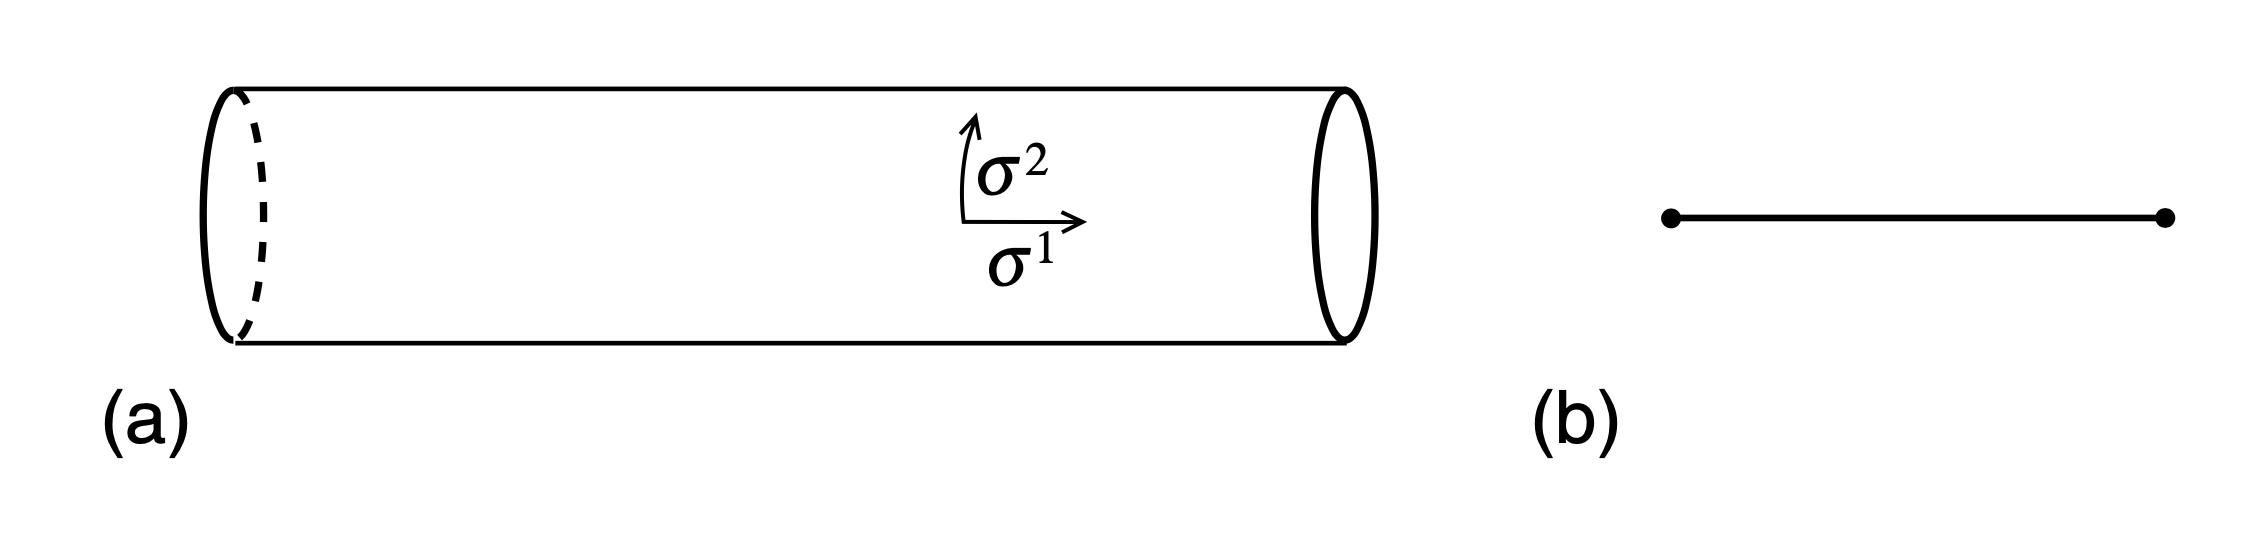
\includegraphics[width=0.6\textwidth]{figure/fig101.png}
		\caption{(a) Cylinder in the small $t$ limit. (b) Field theory analogy diagram.}
	\end{figure}
	
	First examine the cylinder, combined with the results for bosonic strings (\textcolor{red}{7.4.1}) in ten dimensions, plus the fermionic trace (\ref{10.7.9}); the trace here comes from one side of a Type II string, and we write it as a sum of two terms
	\begin{equation}
		Z_{C_{2}}=Z_{C_{2},0}+Z_{C_{2},1} \:, \label{10.8.1}
	\end{equation}
	where
	\begin{subequations}
		\begin{align}
			Z_{C_{2},0}&=\mi V_{10} n^{2}\int^{\infty}_{0}\frac{\dif t}{8t}(8\pi^{2}\alpha^{\prime}t)^{-5}\eta(\mi t)^{-8}
			\Bigl[Z^{0}{}_{0}(\mi t)^{4}-Z^{1}{}_{0}(\mi t)^{4}\Bigr] \:, \label{10.8.2a} \\
			Z_{C_{2},1}&=\mi V_{10} n^{2}\int^{\infty}_{0}\frac{\dif t}{8t}(8\pi^{2}\alpha^{\prime}t)^{-5}\eta(\mi t)^{-8}
			\Bigl[-Z^{0}{}_{1}(\mi t)^{4}-Z^{1}{}_{1}(\mi t)^{4}\Bigr] \:, \label{10.8.2b}
		\end{align} \label{10.8.2}
	\end{subequations}
	(Note that Type I superstrings can only be unoriented; they come from Type IIB string theory, so there is a negative sign in front of $Z^{1}{}_{1}$.) We separated these four terms according to whether $\exp(\pi\mi F)$ appeared in the trace. $\exp(\pi\mi F)$ is not in $Z_{C_{2},0}$, so $\psi^{\mu}$ is antiperiodic in the $\sigma_{2}$ direction. This term is in $Z_{C_{2},1}$, so $\psi^{\mu}$ is periodic in the $\sigma_{2}$ direction. We can also think of the cylinder as closed strings being produced from vacuum and then annihilated back to vacuum. The periodicity of $\psi^{\mu}$ indicates that $Z_{C_{2},0}$ comes from NS-NS strings and $Z_{C_{2},1}$ comes from R-R closed strings.
	
	Due to supersymmetry, the total fermionic string partition function is zero, which makes $Z_{C_{2},1}=-Z_{C_{2},0}$; we now concentrate on $Z_{C_{2},0}$. Using modular transformation
	\begin{equation}
		\eta_{\mi t} =t^{-1/2} \eta(\mi/t) \:, \qquad Z^{\alpha}{}_{\beta}(\mi t) = Z^{\beta}{}_{-\alpha}(\mi/t)\label{10.8.3}
	\end{equation}
	Define $s=\pi/t$, which becomes
	\begin{align}
		Z_{C_{2},0} &= \mi \frac{V_{10}n^{2}}{8\pi(8\pi^{2}\alpha^{\prime})^{5}}
		\int \dif s\:\eta(\mi s/\pi)^{-8}\Bigl[Z^{0}{}_{0}(\mi s/\pi)^{4}- Z^{0}{}_{1}(\mi s/\pi)^{4} \Bigr] \nonumber \\
		&=\mi \frac{V_{10}n^{2}}{8\pi(8\pi^{2}\alpha^{\prime})^{5}}
		\int \dif s\: [16 + O(\exp(-2s))] \:. \label{10.8.4}
	\end{align}
	\begin{tcolorbox}[breakable]
		\begin{remark}
			\textbf{Change of variables.} Apply (\ref{10.8.3}) with $\tau=\mi t\to-1/\tau=\mi/t$. By the box after (\ref{10.7.14}), $Z^0{}_0(\mi t)=Z^0{}_0(\mi/t)$ and $Z^1{}_0(\mi t)=Z^0{}_1(\mi/t)$. Then
			\begin{align*}
				\frac{\dif t}{8t}(8\pi^{2}\alpha't)^{-5}\eta(\mi t)^{-8}
				&\eqs{1}\frac{\dif t}{8t}(8\pi^{2}\alpha')^{-5}t^{-5}\,t^{4}\,\eta(\mi/t)^{-8}
				=\frac{(8\pi^{2}\alpha')^{-5}}{8}\frac{\dif t}{t^{2}}\,\eta(\mi/t)^{-8}\\
				&\eqs{2}\frac{(8\pi^{2}\alpha')^{-5}}{8\pi}\,\dif s\;\eta(\mi s/\pi)^{-8} .
			\end{align*}
			At (1), $\eta(\mi t)^{-8}=t^{4}\eta(\mi/t)^{-8}$. At (2), $s=\pi/t$, so $\dif t/t^{2}=-\dif s/\pi$, and the orientation flip was absorbed by swapping the limits. Together with the bracket $Z^0{}_0{}^4-Z^0{}_1{}^4$, this is the first line of (\ref{10.8.4}).

			\textbf{Large $s$.} Here $\tau=\mi s/\pi$ and $q=\me^{2\pi\mi\tau}=\me^{-2s}$. From the $q$-expansions in the proof after (\ref{10.7.16}),
			\begin{equation*}
				\eta^{-8}\bigl(Z^0{}_0{}^{4}-Z^0{}_1{}^{4}\bigr)=\frac{\vartheta_{00}^{4}-\vartheta_{01}^{4}}{\eta^{12}}=\frac{16q^{1/2}+128q^{3/2}+\cdots}{q^{1/2}\prod(1-q^m)^{8}}=16+O(q)=16+O(\me^{-2s}) .
			\end{equation*}
			The constant $16$ is the massless closed-string state exchanged over the long tube. It gives the divergence $\int^\infty\dif s$. The next term is $\me^{-2s}$, which is the propagation of the first massive level.
		\end{remark}
	\end{tcolorbox}
	Divergence as $s\to\infty$ is due to massless closed string tadpoles; note that this must be an NS-NS state. We view it as dilaton-graviton interaction $(-G)^{1/2}\me^{-\Phi}$.
	
	However, there is a contradiction here: $d=10, N=1$ supersymmetric algebra does not allow such a term. Even more strangely, $Z_{C_{2},1}$ has a divergence of equal size and opposite sign, which can only come from R-R state tadpoles, but the only massless R-R state is a 2nd-order tensor, which cannot have Lorentz-invariant tadpoles.
	
	One can guess the solution is like this. Type IIB strings have $n$-th rank potentials for all even $n$, and $n$ and $8-n$ are equal under Poincaré duality. $\Omega$ projection removed $n=0$ and equivalent $n=8$, as well as $n=4$: all multiples of 4. $n=2$, equivalent $n=6$ and $n=10$ are left. A 10-form potential $C_{10}$ is allowed in 10 dimensions, but its 11-form field strength $\dif C_{10}$ is identically zero. The integration of this potential over spacetime
	\begin{equation}
		\mu_{10}\int C_{10} \label{10.8.5}
	\end{equation}
	is invariant under $\delta C_{10}=\dif \chi_{9}$, so it can appear in action. Because there is no kinetic energy term, the propagator for this field is $1/0$, and the divergence of the tadpole is
	\begin{equation}
		\frac{\mu^{2}_{10}}{0} \:. \label{10.8.6}
	\end{equation}
	This is exactly the origin of divergence in $Z_{C_{2},1}$. The equation of motion given by the variation of $C_{10}$ is $\mu_{10}=0$, so unlike previously encountered divergences, this one cannot be removed by background field corrections. It represents a real incompatibility.
	
	\subsection*{The Klein bottle}
	
	There is another way to cancel tadpole divergences. Cylinders, Mobius strips and Klein bottles all have divergences from massless closed string states, with the total divergence being proportional to the square of the sum of the disk tadpole and the $RP_{2}$ tadpole. The relative size of the two tadpoles depends on the Chan-Paton factors, canceling each other for specific gauge groups.
	
	To sum these contributions, we must readjust these surfaces so that the perimeter in the $\sigma^{2}$ direction and the length in the $\sigma^{1}$ direction are consistent; we take them to be $2\pi$ and $s$, respectively. For the cylinder, the original length of $\sigma^{1}$ was $\pi$ (due to the cylinder corresponding to open strings), and the length in the $\sigma^{2}$ direction was $2\pi t$, so we get $s=\pi/t$; for the Klein bottle $s=\pi/2t$; and for the Mobius strip $s=\pi/4t$. 
	
	Each amplitude is a sum over traces, which come from different boundary conditions and projections. We need to determine which terms contribute to NS-NS exchanges and which contribute to R-R exchanges by examining boundary conditions of fermions on worldsheet path integrals. On the Klein bottle, the GSO projection operator is
	\begin{equation}
		\frac{1+\exp(\pi\mi F)}{2} \:,\qquad \frac{1+\exp(\pi\mi\tilde{F})}{2} \:. \label{10.8.7}
	\end{equation}
	Adding $R=\Omega \exp(\pi\mi\beta F +\pi\mi\tilde{\beta}\tilde{F})$ to the trace, path integral boundary conditions are
	\begin{subequations}
		\begin{align}
			\psi(w+2\pi\mi t)&= -R\psi(w)R^{-1} =-\exp(\pi\mi\beta)\tilde{\psi}(\bar{w}) \:, \label{10.8.8a} \\
			\tilde{\psi}(\bar{w}+2\pi\mi t)&= -R\tilde{\psi}(\bar{w})R^{-1} =-\exp(\pi\mi\tilde{\beta})\psi(w)\:,\label{10.8.8b}
		\end{align} \label{10.8.8}
	\end{subequations}
	negative signs appear because of the fermion field. This gives
	\begin{equation}
		\psi(w+4\pi\mi t) = \exp[\pi\mi(\beta+\tilde{\beta})]\,\psi(w) \:. \label{10.8.9}
	\end{equation}
	NS-NS exchange comes from sectors antisymmetric under $\sigma^{2}\to\sigma^{2}+4\pi t$, and thus from traces factoring in weight $\Omega\exp(\pi\mi F)$ or $\Omega\exp(\pi\mi\tilde{F})$; furthermore, these two traces are equal. Both NS-NS and R-R states contribute to this trace, and their respective contributions are
	\begin{subequations}
		\begin{align}
			\text{NS-NS }: \qquad &q^{-1/3}\prod_{m=1}^{\infty} (1+q^{2m-1})^{8} = Z^{0}{}_{0}(2\mi t)^{4} \:, \label{10.8.10a} \\
			\text{R-R }: \qquad &-16 q^{2/3} \prod_{m=1}^{\infty} (1+q^{2m})^{8} =- Z^{1}{}_{0}(2\mi t)^{4} \:,
			\label{10.8.10b}
		\end{align} \label{10.8.10}
	\end{subequations}
	where $q=\exp(-2\pi t)$.
	
	Thus, the entire Klein bottle contribution to NS-NS exchange is
	\begin{align}
		Z_{K_{2},0} &= \mi V_{10} \int_{0}^{\infty}\frac{\dif t}{8t}\: (4\pi^{2}\alpha^{\prime}t)^{-5} \eta(2\mi t)^{-8}
		\Bigl[ Z^{0}{}_{0}(2\mi t)^{4}-Z^{1}{}_{0}(2\mi t)^{4}\Bigr] \nonumber \\
		&= \mi \frac{2^{10}V_{10}}{8\pi (8\pi^{2}\alpha^{\prime})^{5}}\int^{\infty}_{0}\dif s \: 
		\eta(\mi s/\pi)^{-8} \Bigl[ Z^{0}{}_{0}(\mi s/\pi)^{4}-Z^{1}{}_{0}(\mi s/\pi)^{4} \Bigr] \nonumber \\
		&= \mi \frac{2^{10}V_{10}}{8\pi (8\pi^{2}\alpha^{\prime})^{5}}\int^{\infty}_{0}\dif s \: 
		[16 + O(\exp(-2s))] \:, \label{10.8.11}
	\end{align}
	and $Z_{K_{2},1}=-Z_{K_{2},0}$. The bosonic part is the same as before.
	\begin{tcolorbox}[breakable]
		\begin{remark}
			\textbf{Why $\tau=2\mi t$ in (\ref{10.8.10}).} $\Omega$ exchanges left and right movers, $\Omega\lvert i\rangle_L\lvert j\rangle_R=\pm\lvert j\rangle_L\lvert i\rangle_R$. So in $\operatorname{Tr}\bigl(\Omega\,q^{L_0+\tilde L_0}\bigr)$ only the diagonal states $i=j$ contribute, and each carries $q^{2L_0}=(q^{2})^{L_0}$. The Klein-bottle trace is therefore a single chiral trace at nome $q^{2}=\me^{-4\pi t}$, i.e.\ at $\tau=2\mi t$.

			\textbf{(\ref{10.8.10}).} With $Q\equiv q^{2}$ the nome of $\tau=2\mi t$, and the products of (\ref{10.7.7b}),
			\begin{align*}
				Z^0{}_0(2\mi t)^{4}&=Q^{-1/6}\prod_m(1+Q^{m-1/2})^{8}=q^{-1/3}\prod_m(1+q^{2m-1})^{8},\\
				Z^1{}_0(2\mi t)^{4}&=\bigl(2Q^{1/12}\bigr)^{4}\prod_m(1+Q^{m})^{8}=16q^{2/3}\prod_m(1+q^{2m})^{8} .
			\end{align*}
			The R-R sign is the spacetime statistics of the R sector, as in (\ref{10.7.9}).

			\textbf{(\ref{10.8.11}).} Now $\tau=2\mi t\to-1/\tau=\mi/2t$:
			\begin{align*}
				\frac{\dif t}{8t}(4\pi^{2}\alpha't)^{-5}\eta(2\mi t)^{-8}
				&\eqs{1}\frac{\dif t}{8t}\,2^{5}(8\pi^{2}\alpha')^{-5}t^{-5}\,(2t)^{4}\,\eta(\mi/2t)^{-8}
				=\frac{2^{9}(8\pi^{2}\alpha')^{-5}}{8}\frac{\dif t}{t^{2}}\eta(\mi/2t)^{-8}\\
				&\eqs{2}\frac{2^{10}(8\pi^{2}\alpha')^{-5}}{8\pi}\,\dif s\;\eta(\mi s/\pi)^{-8} .
			\end{align*}
			At (1), $(4\pi^{2}\alpha')^{-5}=2^{5}(8\pi^{2}\alpha')^{-5}$ and $\eta(2\mi t)^{-8}=(2t)^{4}\eta(\mi/2t)^{-8}$. At (2), $s=\pi/2t$, so $\dif t/t^{2}=2\,\dif s/\pi$ up to orientation, and $\mi/2t=\mi s/\pi$. The bracket becomes $Z^0{}_0{}^4-Z^0{}_1{}^4$ at $\mi s/\pi$, exactly as for the cylinder, which gives the same $16+O(\me^{-2s})$. So the Klein bottle is the cylinder result with $n^{2}\to2^{10}=32^{2}$.
		\end{remark}
	\end{tcolorbox}
	
	
	\subsection*{The M\"{o}bius strip}
	
	In open strings, the effect of $\Omega$ is
	\begin{equation}
		\Omega\psi^{\mu}(w)\Omega^{-1} =\tilde{\psi}(\pi-\bar{w})=\psi^{\mu}(w-\pi) \:,\label{10.8.12}
	\end{equation}
	doubling trick (\ref{10.2.15}) was used here. In form of oscillator modes, this is
	\begin{equation}
		\Omega \psi^{\mu}_{r} \Omega^{-1} =\exp(-\pi\mi r) \,\psi_{r}^{\mu} \:. \label{10.8.13}
	\end{equation}
	This phase is imaginary and its square is equal to $-1$ in the NS sector. Therefore,
	\begin{equation}
		\Omega^{2} =\exp(\pi\mi F) \:. \label{10.8.14}
	\end{equation}
	\begin{tcolorbox}[breakable]
		\begin{remark}
			\textbf{(\ref{10.8.13}).} With the doubled field of (\ref{10.2.15}) and the expansion (\ref{10.2.5}),
			\begin{equation*}
				\Omega\psi^\mu(w)\Omega^{-1}=\psi^\mu(w-\pi)=\mi^{-1/2}\sum_r\psi^\mu_r\me^{\mi r(w-\pi)}
				\quad\Longrightarrow\quad \Omega\psi^\mu_r\Omega^{-1}=\me^{-\pi\mi r}\psi^\mu_r .
			\end{equation*}
			\textbf{(\ref{10.8.14}).} Applying this twice gives $\Omega^{2}\psi_r\Omega^{-2}=\me^{-2\pi\mi r}\psi_r$. This is $-\psi_r$ for $r\in\mathds Z+\tfrac12$ and $+\psi_r$ for $r\in\mathds Z$. On NS states $\Omega^{2}$ therefore gives $-1$ per $\psi$ excitation, which is the action of $\exp(\pi\mi F)$ on them. The phase of $\Omega$ on the ground state is a convention, fixed so that (\ref{10.8.14}) holds on all states. $\Omega$ is then of order 4 on the full space, which is why the projector (\ref{10.8.15}) averages over $\Omega^{0,1,2,3}$. On GSO-projected states it reduces to $\tfrac12(1+\Omega)$.

			\textbf{(\ref{10.8.16}).} In the trace with $R=\Omega\exp(\pi\mi\beta F)$, going once around the $\sigma^{2}$ circle of circumference $2\pi t$ gives $\psi(w+2\pi\mi t)=-\exp(\pi\mi\beta)\,\psi(w-\pi)$. The $-$ is the fermionic trace, and the argument is from (\ref{10.8.12}). Going around twice,
			\begin{equation*}
				\psi(w+4\pi\mi t)=-\me^{\pi\mi\beta}\psi(w+2\pi\mi t-\pi)=\bigl(-\me^{\pi\mi\beta}\bigr)^{2}\psi(w-2\pi)=\psi(w-2\pi),
			\end{equation*}
			for $\beta\in\{0,1\}$. By (\ref{10.2.3a}), $\psi(w-2\pi)=\me^{-2\pi\mi\nu}\psi(w)$. So along the doubled $\sigma^{2}$ circle, which is the closed-string time direction of the M\"obius strip, R-sector fields ($\nu=0$) are periodic and NS-sector fields are antiperiodic. In the closed-string channel the R sector of the open-string trace is R-R exchange, and the NS sector is NS-NS exchange.
		\end{remark}
	\end{tcolorbox}
	According to GSO projection, $\exp(\pi\mi F)=1$; physically, its square is the same as the identity operator, but the combined projection of $\Omega$ and GSO requires
	\begin{equation}
		\frac{1+\Omega +\Omega^{2}+\Omega^{3}}{4} \:. \label{10.8.15}
	\end{equation}
	Now there's $R=\Omega \exp(\pi\mi\beta F)$ in the trace, and the periodicity of the field is
	\begin{equation}
		\psi^{\mu}(w+4\pi\mi t) = -\exp(\pi\mi\beta)\psi^{\mu}(w+2\pi\mi t-\pi) =\psi^{\mu}(w-2\pi) \:. \label{10.8.16}
	\end{equation}
	It follows that in the R sector of trace, the field is periodic in the $\sigma^{2}$ direction, corresponding to R-R exchange, while the NS sector of trace gives NS-NS exchange.
	
	R-R exchange is simpler, and the sum of traces containing $\Omega$ and $\Omega\exp(\pi\mi F)$ is
	\begin{align}
		-16q^{1/3}&\prod_{m=1}^{\infty} [1+(-1)^{m}q^{m}]^{8} 
		-(1-1)^{4}q^{1/3}\prod_{m=1}^{\infty} [1-(-1)^{m}q^{m}]^{8} \nonumber \\
		&= Z^{0}{}_{1}(2\mi t)^{4} Z^{1}{}_{0}(2\mi t)^{4} \:. \label{10.8.17}
	\end{align}
	The overall Mobius amplitude is
	\begin{align}
		Z_{M_{2},1}&=\pm\mi n V_{10} \int_{0}^{\infty} \frac{\dif t}{8t}(8\pi^{2}\alpha^{\prime}t)^{-5}
		\frac{Z^{0}{}_{1}(2\mi t)^{4}Z^{1}{}_{0}(2\mi t)^{4}}{\eta(2\mi t)^{8}Z^{0}{}_{0}(2\mi t)^{4}}\nonumber \\
		&=\pm 2\mi n \frac{2^{5}V_{10}}{8\pi(8\pi^{2}\alpha^{\prime})^{5}}\int_{0}^{\infty}\dif s \:
		\frac{Z^{0}{}_{1}(2\mi s/\pi)^{4}Z^{1}{}_{0}(2\mi s/\pi)^{4}}{\eta(2\mi s/\pi)^{8}Z^{0}{}_{0}(2\mi s/\pi)^{4}}\nonumber \\
		&=\pm 2\mi n \frac{2^{5}V_{10}}{8\pi(8\pi^{2}\alpha^{\prime})^{5}}\int_{0}^{\infty}\dif s \:
		[16+O(\exp(-2s))] \:, \label{10.8.18}
	\end{align}
	where the positive sign corresponds to $SO(n)$.
	
	The total divergence of R-R exchange is
	\begin{equation}
		Z_{1} = -\mi(n\mp 32)^{2} \frac{V_{10}}{8\pi (8\pi^{2}\alpha^{\prime})^{5}}
		\int^{\infty}_{0}\dif s \:[16+O(\exp(-2s))] \:. \label{10.8.19}
	\end{equation}
	\begin{tcolorbox}[breakable]
		\begin{remark}
			\textbf{Conventions.} Open-string traces are at $q=\me^{-2\pi t}$, with the eight transverse directions. $Q\equiv q^{2}$ is the nome at $\tau=2\mi t$. By (\ref{10.8.13}), $\Omega$ multiplies an integer mode $n$ by $(-1)^n$, and the same holds for the $X$ oscillators.

			\textbf{The R-R trace (\ref{10.8.17}).} The R ground states carry $2^{8/2}=16$ states and zero-point energy $8\cdot\tfrac1{24}=\tfrac13$, and the spacetime statistics give a $-$ sign. In the $\Omega\exp(\pi\mi F)$ trace the zero modes give $\operatorname{Tr}_{16}\Gamma=0$, which is the $(1-1)^{4}$. The surviving piece, times the bosonic M\"obius trace $q^{-1/3}\prod_m(1-(-1)^mq^m)^{-8}$, is
			\begin{align*}
				-16\prod_m\Bigl[\frac{1+(-1)^mq^m}{1-(-1)^mq^m}\Bigr]^{8}
				&\eqs{1}-16\prod_m\Bigl[\frac{(1+Q^{m})(1-Q^{m-1/2})}{(1-Q^{m})(1+Q^{m-1/2})}\Bigr]^{8}\\
				&\eqs{2}-\frac{Z^0{}_1(2\mi t)^{4}\,Z^1{}_0(2\mi t)^{4}}{\eta(2\mi t)^{8}\,Z^0{}_0(2\mi t)^{4}} .
			\end{align*}
			At (1), the even $m=2k$ and odd $m=2k-1$ factors were separated, with $q^{2k}=Q^{k}$ and $q^{2k-1}=Q^{k-1/2}$. At (2), the products of (\ref{10.7.7b}) at nome $Q$ were used: $Z^0{}_1{}^4Z^1{}_0{}^4/Z^0{}_0{}^4=16\,Q^{1/3}\prod(1+Q^m)^{8}(1-Q^{m-1/2})^{8}(1+Q^{m-1/2})^{-8}$ and $\eta^{8}=Q^{1/3}\prod(1-Q^m)^{8}$.

			\textbf{Printed-equation note.} (\ref{10.8.17}) as printed equates the fermionic trace alone to $Z^0{}_1{}^4Z^1{}_0{}^4$. The identity holds only after the bosonic M\"obius trace is included, and then with the ratio above, which is what enters (\ref{10.8.18}). The overall sign is absorbed into the $\pm$ of (\ref{10.8.18}), which is fixed by the $SO/Sp$ action of $\Omega$ on the Chan--Paton factors.

			\textbf{(\ref{10.8.18}).} With $\tau=2\mi t\to\mi/2t$, the ratio of $Z$'s is invariant because $Z^0{}_1\leftrightarrow Z^1{}_0$. Then
			\begin{align*}
				\frac{\dif t}{8t}(8\pi^{2}\alpha't)^{-5}\eta(2\mi t)^{-8}
				&\eqs{1}\frac{2^{4}(8\pi^{2}\alpha')^{-5}}{8}\frac{\dif t}{t^{2}}\eta(\mi/2t)^{-8}
				\eqs{2}\frac{2\cdot2^{5}(8\pi^{2}\alpha')^{-5}}{8\pi}\dif s\;\eta(2\mi s/\pi)^{-8} .
			\end{align*}
			At (1), $\eta(2\mi t)^{-8}=(2t)^{4}\eta(\mi/2t)^{-8}$. At (2), $s=\pi/4t$, so $\dif t/t^{2}=4\,\dif s/\pi$ and $\mi/2t=2\mi s/\pi$. At large $s$ the nome is $\me^{-4s}$. $\eta^{-8}Z^1{}_0{}^4=16(1+\cdots)$ and $Z^0{}_1{}^4/Z^0{}_0{}^4=1+O(\me^{-2s})$, so the bracket is $16+O(\me^{-2s})$.

			\textbf{(\ref{10.8.19}).} Using $Z_{C_2,1}=-Z_{C_2,0}$ and $Z_{K_2,1}=-Z_{K_2,0}$, with the common factor $\frac{\mi V_{10}}{8\pi(8\pi^{2}\alpha')^{5}}\int\dif s\,[16+\cdots]$ written as $\mi\mathcal N$:
			\begin{equation*}
				Z_1=-\mi\mathcal N\bigl(n^{2}+2^{10}\bigr)\pm\mi\mathcal N\,2\cdot2^{5}n=-\mi\mathcal N\bigl(n^{2}\mp64n+1024\bigr)=-\mi\mathcal N\,(n\mp32)^{2} .
			\end{equation*}
			The upper sign is $SO(n)$. The R-R tadpole cancels only for $SO(32)$: the three surfaces combine into a perfect square because the divergence is (disk tadpole $+$ $RP_2$ tadpole)$^{2}$.
		\end{remark}
	\end{tcolorbox}
	The R-R tadpole is zero for the gauge group $SO(32)$. For each worldsheet topology, NS-NS divergence is the negative of the R-R divergence, so dilaton-graviton tadpoles are also zero for $SO(32)$.
	\chapter{\texorpdfstring{Heterotic Strings}{11 Heterotic Strings}} \label{cha:11}

\section{World-sheet Supersymmetry} \label{sec:11.1}

In the previous chapter, we saw the method of expanding the world-sheet constraint algebra by adding supercurrents $T_{F}(z)$ and $\tilde{T}_{F}(\bar{z})$. Now we look at how far this idea can go—specifically, seeking a set of holomorphic or antiholomorphic currents such that their Laurent coefficients form a closed algebra.

We first specify the difference between global symmetries and constraints. Global symmetries on the world-sheet are like global symmetries in spacetime; they imply relationships between masses and amplitudes. However, we usually also pick out a portion of the symmetries as \emph{constraints} to be attached to the system, meaning that physical states must be annihilated by these constraints. In the bosonic string, spacetime Poincaré symmetry is a global symmetry of the world-sheet theory, while conformal symmetry is a constraint. Our current interest is in constraint algebras. In fact, the possible sets we find are very small, but later we will encounter some additive algebras that appear as global symmetries.

First, it should be noted that the collection of sets capable of acting as world-sheet symmetry algebras is very large. For example, in the bosonic string, any product of factors $\partial^{n}X^{\mu}$ is a holomorphic current. In most cases, the OPE of such currents will generate an infinite number of new currents. Even if restricted to a finite number of currents, infinite possibilities still remain.

We first concentrate on holomorphic currents. In a unitary CFT, a primary operator can be holomorphic only if its weight is $(h,0)$ with $h>0$ (holomorphicity requires $\tilde{h}=0$, and unitarity gives $h>0$). Although the complete world-sheet theory lacks a positive-definite norm due to ghost fields and timelike oscillators, the spatial part is indeed unitary, so it resides in a unitary representation of the symmetry. Since $\tilde{h}=0$, the spin of the current is also equal to $h$. (Note that $h+\tilde{h}$ determines the scaling behavior of the current, while $h-\tilde{h}$ determines the rotation behavior, because $z\bar{z}=r^{2}$ and $z/\bar{z}=\me^{2\mi\varphi}$, where $z=r\me^{\mi\varphi}$). We assume the currents are Hermitian and now examine the following possibilities:

\emph{Spin} $h\geq 2$: For algebras of currents with spin $>2$, we usually call them $W$-\emph{algebras}. Most are known, including several classes of infinite algebras, but there is no complete classification yet. There have been attempts to use some of these algebras as constraint algebras. One difficulty is that the commutators of the generators are generally non-linear functions of the generators, which makes the construction of the BRST operator very non-trivial. A few constructed examples were found after gauge fixing to be just special cases of the bosonic string. Another difficulty is that the geometric interpretation is unclear. So we will focus our attention on algebras with $h\leq 2$. Additionally, a CFT can possess multiple $(2,0)$ currents as global symmetries. The bosonic string has at least 27, namely the energy-momentum tensor of the ghost fields and the energy-momentum tensors of the 26 $X^{\mu}$ fields. However, only their sum has a geometric interpretation as conformal invariance; therefore, we will assume there is only one $(2,0)$ constraint current, namely the total energy-momentum tensor.

\emph{Spin $h$ is not an integer multiple of $\frac{1}{2}$}: For a current $j$ with spin $h$,
\begin{equation}
	j(z)j(0)\sim z^{-2h} \label{11.1.1}
\end{equation}
If $2h$ is not an integer, this will be multi-valued. Although many CFTs are already known to possess such currents, difficulties arise from non-locality when we try to use such currents as constraints. Attempts to construct such \emph{fractional strings} have yielded partial results, but whether such theories exist remains unclear. So we restrict $h$ to be an integer multiple of $\frac{1}{2}$.

With these constraints, the possible algebras are greatly restricted; the spin can only be $0, \frac{1}{2}, 1, \frac{3}{2}, 2$. The algebras allowed by the Jacobi identity are listed in Table \ref{tab:11.1}. The first two are obviously the conformal algebra and the $N=1$ superconformal algebra we have studied. The three $N=4$ algebras are related to each other. Among them, the second algebra is a special case of the first algebra, where the $U(1)$ current of the first algebra is the gradient of some scalar. The third is a subalgebra of the second.

\begin{table}[ht]
	\caption{World-sheet superconformal algebras. The table lists the number of currents of each spin, the total ghost central charge, the global symmetries generated by spin-1 currents, and the transformations of supercharges under these symmetries.}
	\label{tab:11.1}%
	\centering
	\begin{tabular}[c]{cccccll}
		\hline\hline
		$\vphantom{\Big[}n_{3/2}=N$ & $n_{1}$ & $n_{1/2}$ & $n_{0}$ & $c^{\text{g}}$ & symmetry & $T_{F}\:$rep. \\
		\hline
		0 & 0 & 0 & 0 & $-26$ & &  \\
		1 & 0 & 0 & 0 & $-15$ & &  \\
		2 & 1 & 0 & 0 & $-6$ & $U(1)$ & $\pm1$  \\
		3 & 3 & 1 & 0 & 0 & $SU(2)$ & $\mathbf{3}$  \\
		4 & 7 & 4 & 0 & 0 & $SU(2)\times SU(2)\times U(1)$ & $(\mathbf{2},\mathbf{2},0)$  \\
		4 & 6 & 4 & 1 & 0 & $SU(2)\times SU(2)$ & $(\mathbf{2},\mathbf{2})$  \\
		4 & 3 & 0 & 0 & 12 & $SU(2)$ & $\mathbf{2}$  \\
		\hline\hline
	\end{tabular}
\end{table}

The ghost central charge is determined by the number of currents of each spin; the ghost central charge associated with a current of spin $h$ is
\begin{subequations}
	\begin{align}
		c_{h}&=(-1)^{2h+1}[3(2h-1)^{2}-1] \: , \label{11.1.2a} \\
		c_{2}&=-26\:,\qquad c_{3/2}=+11\:,\qquad c_{1}=-2\:,\qquad c_{1/2}=-1\:, \qquad c_{0}=-2\:. \label{11.1.2b}
	\end{align} \label{11.1.2}
\end{subequations}
The sign $(-1)^{2h+1}$ is the result of taking the statistics of the ghost fields into account, anticommuting for integer spin and commuting for half-integer spin. Since the matter field central charge $c^{\text{m}}$ is $-c^{\text{g}}$, only one new algebra has a critical dimension, namely $N=2$.
\begin{tcolorbox}[breakable]
	\begin{remark}
		Gauge fixing a constraint current of weight $h$ introduces a ghost pair: an antighost $b$ of weight $\lambda=h$ (it has the same indices as the current) and a ghost $c$ of weight $1-h$. The pair has the opposite statistics to the current, so it is Grassmann odd for integer $h$ and Grassmann even for half-integer $h$. The central charges of the two kinds of pair are \eqref{2.5.12} and its commuting analogue,
		\begin{equation*}
			c_{bc}=-3(2\lambda-1)^{2}+1\:,\qquad c_{\beta\gamma}=+3(2\lambda-1)^{2}-1\:,
		\end{equation*}
		so with $\lambda=h$,
		\begin{align*}
			c_{h}=\begin{cases} -[3(2h-1)^{2}-1] & h\in\mathds{Z} \\ +[3(2h-1)^{2}-1] & h\in\mathds{Z}+\tfrac{1}{2}\end{cases}
			\;=(-1)^{2h+1}\bigl[3(2h-1)^{2}-1\bigr]\:.
		\end{align*}
		Evaluating,
		\begin{align*}
			c_{2}&=-(27-1)=-26\:,& c_{3/2}&=+(12-1)=11\:,& c_{1}&=-(3-1)=-2\:,\\
			c_{1/2}&=+(0-1)=-1\:,& c_{0}&=-(3-1)=-2\:.
		\end{align*}
		The ghost central charges in Table \ref{tab:11.1} follow from $c^{\text{g}}=c_{2}+n_{3/2}c_{3/2}+n_{1}c_{1}+n_{1/2}c_{1/2}+n_{0}c_{0}$:
		\begin{align*}
			N=2&: \quad -26+2(11)+1(-2)=-6\:, \\
			N=3&: \quad -26+3(11)+3(-2)+1(-1)=0\:, \\
			N=4\ (7,4,0)&: \quad -26+4(11)+7(-2)+4(-1)=0\:, \\
			N=4\ (6,4,1)&: \quad -26+4(11)+6(-2)+4(-1)+1(-2)=0\:, \\
			N=4\ (3,0,0)&: \quad -26+4(11)+3(-2)=12\:.
		\end{align*}
		A critical dimension requires $c^{\text{m}}=-c^{\text{g}}>0$, which among the new algebras happens only for $N=2$, with $c^{\text{m}}=6$.
	\end{remark}
\end{tcolorbox}

For $N=2$, it is convenient to combine two real supercurrents into one complex supercurrent
\begin{equation}
	T_{F}^{\pm} = 2^{-1/2}(T_{F1}\pm \mi T_{F2}) \:. \label{11.1.3}
\end{equation}
In this way, the $N=2$ algebra in operator product form is
\begin{subequations}
	\begin{align}
		T_{B}(z)T_{F}^{\pm}(0)&\sim \frac{3}{2z^{2}} T_{F}^{\pm}(0) + \frac{1}{z}\partial T_{F}^{\pm}(0)\:,\label{11.1.4a} \\
		T_{B}(z) j(0) &\sim \frac{1}{z^{2}} j(0) +\frac{1}{z}\partial j(0) \:, \label{11.1.4b} \\
		T_{F}^{+}(z)T_{F}^{-}(0)&\sim \frac{2c}{3z^{3}}+\frac{2}{z^{2}}j(0)+\frac{2}{z}T_{B}(0)+\frac{1}{z}\partial j(0) \:,\label{11.1.4c} \\
		T^{+}_{F}(z)T^{+}_{F}(0)& \sim T^{-}_{F}(z)T^{-}_{F}(0) \sim 0 \:, \label{11.1.4d} \\
		j(z)T_{F}^{\pm}(0) &\sim \pm \frac{1}{z} T_{F}^{\pm}(0) \:, \label{11.1.4e} \\
		j(z)j(0) &\sim \frac{c}{3z^{2}}\:. \label{11.1.4f}
	\end{align}
\end{subequations}
This implies that $T_{F}^{\pm}$ and $j$ are primary fields, and $T_{F}^{\pm}$ possesses charges $\pm1$ under the $U(1)$ generated by $j$. According to the Jacobi identity, the constant $c$ in $T_{F}^{+}T_{F}^{-}$ and $jj$ must be the central charge.

The minimal linear representation of the $N=2$ algebra possesses two real scalar fields and two fermions; we combine them into a complex scalar $Z$ and a complex fermion $\psi$. The action is
\begin{equation}
	S=\frac{1}{2\pi} \int \dif^{2}z\Bigl( \partial \overline{Z}\bar{\partial}Z 
	+\overline{\psi}\bar{\partial}\psi + \tilde{\overline{\psi}}\partial\tilde{\psi}\Bigr)\:. \label{11.1.5}
\end{equation}
The currents are
\begin{subequations}
	\begin{align}
		T_{B} &= -\partial \overline{Z}\partial Z -\frac{1}{2}(\overline{\psi}\partial\psi+\psi\partial\overline{\psi})\:,\qquad j=-\overline{\psi}\psi \:,\label{11.1.6a} \\
		T_{F}^{+} &= 2^{1/2} \mi\psi \partial\overline{Z} \:, \qquad 
		T_{F}^{-} = 2^{1/2} \mi\overline{\psi} \partial Z\:. \label{11.1.6b}
	\end{align} \label{11.1.6}
\end{subequations}
Simultaneously, antiholomorphic currents also exist, so this $Z\psi\tilde{\psi}$ CFT possesses $(2,2)$ superconformal symmetry.
\begin{tcolorbox}[breakable]
	\begin{remark}
		We check that the currents (\ref{11.1.6}) realize the algebra (\ref{11.1.4a})--(\ref{11.1.4f}) with $c=3$. First the propagators. Write $Z=2^{-1/2}(X^{1}+\mi X^{2})$ and $\psi=2^{-1/2}(\psi^{1}+\mi\psi^{2})$. Then
		\begin{align*}
			\partial\overline{Z}\bar{\partial}Z &\eqs{1} \tfrac{1}{2}\bigl(\partial X^{1}\bar{\partial}X^{1}+\partial X^{2}\bar{\partial}X^{2}\bigr)+\tfrac{\mi}{2}\bigl(\partial X^{1}\bar{\partial}X^{2}-\partial X^{2}\bar{\partial}X^{1}\bigr)\:, \\
			\overline{\psi}\bar{\partial}\psi &\eqs{2} \tfrac{1}{2}\bigl(\psi^{1}\bar{\partial}\psi^{1}+\psi^{2}\bar{\partial}\psi^{2}\bigr)+\tfrac{\mi}{2}\,\bar{\partial}\bigl(\psi^{1}\psi^{2}\bigr)\:.
		\end{align*}
		At (1) the imaginary part is $\tfrac{\mi}{2}[\partial(X^{1}\bar{\partial}X^{2})-\bar{\partial}(X^{1}\partial X^{2})]$, a total derivative. At (2) the cross terms $\psi^{1}\bar{\partial}\psi^{2}-\psi^{2}\bar{\partial}\psi^{1}=\psi^{1}\bar{\partial}\psi^{2}+(\bar{\partial}\psi^{1})\psi^{2}$ also form a total derivative. So (\ref{11.1.5}) is $\frac{1}{4\pi}\int\dif^{2}z\,(\partial X^{i}\bar{\partial}X^{i}+\psi^{i}\bar{\partial}\psi^{i}+\cdots)$, the usual free action with $\alpha'=2$, and $X^{i}X^{j}\sim-\delta^{ij}\ln\lvert z\rvert^{2}$, $\psi^{i}\psi^{j}\sim\delta^{ij}/z$. Recombining,
		\begin{equation*}
			\partial\overline{Z}(z)\,\partial Z(0)\sim-\frac{1}{z^{2}}\:,\quad \partial Z\,\partial Z\sim 0\:,\qquad
			\psi(z)\overline{\psi}(0)\sim\overline{\psi}(z)\psi(0)\sim\frac{1}{z}\:,\quad \psi\psi\sim\overline{\psi}\,\overline{\psi}\sim0\:.
		\end{equation*}
		\textbf{The $jj$ and $jT_F$ OPEs.} With $j=-\overline{\psi}\psi$,
		\begin{align*}
			j(z)j(0)&=\overline{\psi}\psi(z)\,\overline{\psi}\psi(0)
			\eqs{1}\frac{1}{z^{2}}+\frac{1}{z}\Bigl[:\!\overline{\psi}(z)\psi(0)\!:+:\!\psi(z)\overline{\psi}(0)\!:\Bigr]+\cdots
			\eqs{2}\frac{1}{z^{2}}+O(z^{0})\:,\\
			j(z)\psi(0)&=-\overline{\psi}\psi(z)\,\psi(0)\eqs{3}+\overline{\psi}(z)\psi(0)\,\psi(z)\sim\frac{1}{z}\psi(0)\:,\qquad
			j(z)\overline{\psi}(0)\sim-\frac{1}{z}\overline{\psi}(0)\:.
		\end{align*}
		At (1) the double contraction pairs $\overline{\psi}(z)$ with $\psi(0)$ and $\psi(z)$ with $\overline{\psi}(0)$; the pairs are nested, so there is no sign. At (2) the two single-contraction terms add to $:\!\overline{\psi}\psi+\psi\overline{\psi}\!:=0$ at $z\to0$, so there is no $1/z$ term, as expected for an abelian current. Thus $c/3=1$ and $c=3$. At (3) $\psi(0)$ was moved past $\psi(z)$, which costs a sign, to sit next to $\overline{\psi}(z)$. So $\psi$ has charge $+1$ and $\overline{\psi}$ charge $-1$. The $Z$ fields are neutral, so $T_{F}^{+}\propto\psi\partial\overline{Z}$ has charge $+1$ and $T_{F}^{-}$ has charge $-1$, which is (\ref{11.1.4e}).

		\textbf{The $T_F^+T_F^-$ OPE.} Bosons commute with fermions, so
		\begin{align*}
			T_{F}^{+}(z)T_{F}^{-}(0)&=-2\,\psi(z)\overline{\psi}(0)\;\partial\overline{Z}(z)\partial Z(0)\\
			&\eqs{1}-2\Bigl(\frac{1}{z}\Bigr)\Bigl(-\frac{1}{z^{2}}\Bigr)-\frac{2}{z}:\!\partial\overline{Z}\partial Z\!:(0)+\frac{2}{z^{2}}:\!\psi(z)\overline{\psi}(0)\!:\\
			&\eqs{2}\frac{2}{z^{3}}+\frac{2}{z^{2}}:\!\psi\overline{\psi}\!:(0)+\frac{1}{z}\Bigl[2:\!\partial\psi\,\overline{\psi}\!:-2:\!\partial\overline{Z}\partial Z\!:\Bigr](0)\\
			&\eqs{3}\frac{2c}{3z^{3}}+\frac{2}{z^{2}}j(0)+\frac{1}{z}\bigl[2T_{B}(0)+\partial j(0)\bigr]\:.
		\end{align*}
		At (1) the three terms are the double contraction, the fermion contraction alone, and the boson contraction alone. At (2) $\psi(z)$ was Taylor expanded about $0$. At (3) $:\!\psi\overline{\psi}\!:=-\overline{\psi}\psi=j$ and $c=3$ were used. The $1/z$ term needs the identity
		\begin{align*}
			2T_{B}+\partial j&=-2\partial\overline{Z}\partial Z-\overline{\psi}\partial\psi-\psi\partial\overline{\psi}-\partial\overline{\psi}\,\psi-\overline{\psi}\partial\psi\\
			&\eqs{4}-2\partial\overline{Z}\partial Z-2\overline{\psi}\partial\psi
			=-2\partial\overline{Z}\partial Z+2\partial\psi\,\overline{\psi}\:,
		\end{align*}
		where at (4) $\psi\partial\overline{\psi}=-\partial\overline{\psi}\,\psi$ cancels the third and fourth terms. Finally $T_{F}^{+}T_{F}^{+}\propto\psi\psi\,\partial\overline{Z}\partial\overline{Z}\sim0$ because neither factor has a contraction, which is (\ref{11.1.4d}).

		\textbf{Primarity.} $\psi$ has weight $\frac12$ and $\partial Z$ has weight $1$, so $T_{F}^{\pm}$ are weight-$\frac{3}{2}$ primaries. For $j$, the only possible anomalous term in $T_{B}j$ is the $z^{-3}$ double contraction with $T_{\psi}=-\frac{1}{2}(\overline{\psi}\partial\psi+\psi\partial\overline{\psi})$:
		\begin{align*}
			\overline{\psi}\partial\psi(z)\,\overline{\psi}\psi(0)\big|_{z^{-3}}&=\Bigl(\partial_{z}\frac{1}{z}\Bigr)\frac{1}{z}=-\frac{1}{z^{3}}\:,\qquad
			\psi\partial\overline{\psi}(z)\,\overline{\psi}\psi(0)\big|_{z^{-3}}\eqs{5}-\frac{1}{z}\Bigl(\partial_{z}\frac{1}{z}\Bigr)=+\frac{1}{z^{3}}\:.
		\end{align*}
		At (5) the contractions $\psi(z)\overline{\psi}(0)$ and $\partial\overline{\psi}(z)\psi(0)$ cross, which gives a minus sign. The two terms cancel, so $T_{B}j$ has no $z^{-3}$ term and $j$ is a weight-1 primary, which is (\ref{11.1.4b}).
	\end{remark}
\end{tcolorbox}

The central charge of the $Z\psi\tilde{\psi}$ CFT is 3, so two such CFTs will cancel the ghost central charge. Since there are two real scalar fields in each CFT, the critical dimension is 4. However, these dimensions combine into complex pairs, so spacetime can only be pure Euclidean space or $(2,2)$ spacetime, and cannot be Minkowski $(3,1)$ spacetime. Furthermore, this theory only has 4-dimensional translation invariance but lacks 4-dimensional Lorentz invariance. The symmetry here is $U(2)$ or $U(1,1)$. Finally, the spectrum here is very small. Constraints completely determine the two sets of $Z\psi\tilde{\psi}$ oscillators. Therefore, only the center-of-mass motion of the singlet remains. This has some mathematical interest, but whether it has physical applications remains unclear.

Thus we return to the original $N=0$ and $N=1$ algebras. However, there is another generalization, where the left-moving and right-moving sectors of the closed string have different algebras. Holomorphic and antiholomorphic algebras commute with each other, so there is no reason they must be equal. In open strings, boundary conditions relate the holomorphic and antiholomorphic parts together, so open strings do not have a similar construction.

This gives a new possibility, $(N,\tilde{N})=(0,1)$ \emph{heterotic strings}; $(N,\tilde{N})=(1,0)$ is isomorphic to it and will not be examined separately. Additionally, $(0,2)$ heterotic string theory and $(1,2)$ heterotic string theory have some mathematical interest.

It should be emphasized that the analysis in this section has many explicit and implicit assumptions, and these assumptions should be treated with caution until we find all string theories. In fact, there are indeed some theories that do not fall into this classification. One is the Green-Schwarz form of superstrings. They do not have simple covariant gauge fixing, but in light-cone gauge, it can be proved via bosonization that they are actually equivalent to RNS superstrings. Another exception is \emph{topological string theory}, which does not satisfy the spin-statistics we assumed under covariant constraints. This string theory has no physical degrees of freedom, but because its observables are topological, it has some interesting mathematical applications.

\section{$SO(32)$ and $E_{8}\times E_{8}$ Heterotic Strings} \label{sec:11.2}

The $(0,1)$ heterotic string combines the ghost fields and constraints of the left-moving bosonic string and the right-moving Type II string. In fact, we can go further and combine the left-moving bosonic string and the right-moving Type II string such that the left side has 26 flat dimensions and the right side has 10 flat dimensions. This is achievable, but its physical meaning is unclear, so we keep the same dimensions on both sides. Thus it is 10. We start from the following fields
\begin{equation}
	X^{\mu}(z,\bar{z})\:,\qquad \tilde{\psi}^{\mu}(\bar{z}) \:, \qquad \mu = 0,\cdots,9\:, \label{11.2.1}
\end{equation}
The total central charge is $(c,\tilde{c})=(10,15)$. The ghost central charge is $(c^{\text{g}},\tilde{c}^{\text{g}})=(-26,-15)$, so the remaining matter fields have $(c,\tilde{c})=(16,0)$. The simplest possibility is to take 32 left-moving spin-$\frac{1}{2}$ fields
\begin{equation}
	\lambda^{A}(z) \:, \qquad A=1,\cdots,32\:. \label{11.2.2}
\end{equation}
The total matter field action is
\begin{equation}
	S=\frac{1}{4\pi} \int \dif^{2}z\: \biggl( \frac{2}{\alpha^{\prime}}\partial X^{\mu}\bar{\partial}X_{\mu}
	+\lambda^{A}\bar{\partial}\lambda^{A}+\tilde{\psi}^{\mu}\partial\tilde{\psi}_{\mu}\biggr)\:.\label{11.2.3}
\end{equation}
The operator products are
\begin{subequations}
	\begin{align}
		X^{\mu}(z,\bar{z})X^{\nu}(0,0) &\sim -\eta^{\mu\nu} \frac{\alpha^{\prime}}{2} \ln\lvert z\rvert^{2} \:,\label{11.2.4a} \\
		\lambda^{A}(z)\lambda^{B}(z) &\sim \delta^{AB}\frac{1}{z} \:, \label{11.2.4b} \\
		\tilde{\psi}^{\mu}(\bar{z})\tilde{\psi}^{\nu}(0) &\sim \eta^{\mu\nu}\frac{1}{\bar{z}} \:.\label{11.2.4c}
	\end{align}
\end{subequations}
The energy-momentum tensor and supercurrent are
\begin{subequations}
	\begin{align}
		T_{B} &= -\frac{1}{\alpha^{\prime}}\partial X^{\mu}\partial X_{\mu} -\frac{1}{2}\lambda^{A}\partial\lambda^{A}\:,\label{11.2.5a} \\
		\tilde{T}_{B}&= -\frac{1}{\alpha^{\prime}}\bar{\partial}X^{\mu}\bar{\partial}X_{\mu} 
		-\frac{1}{2}\tilde{\psi}^{\mu}\bar{\partial}\tilde{\psi}_{\mu} \:, \label{11.2.5b} \\
		\tilde{T}_{F}&= \mi(2/\alpha^{\prime})^{1/2}\tilde{\psi}^{\mu}\bar{\partial}X_{\mu} \:.\label{11.2.5c}
	\end{align} \label{11.2.5}
\end{subequations}
\begin{tcolorbox}[breakable]
	\begin{remark}
		Each free boson contributes $1$ to the central charge and each real fermion $\frac{1}{2}$, so
		\begin{equation*}
			c=10+32\cdot\tfrac{1}{2}=26\:,\qquad \tilde{c}=10+10\cdot\tfrac{1}{2}=15\:,
		\end{equation*}
		which cancel the ghosts $(c^{\text{g}},\tilde{c}^{\text{g}})=(-26,-15)$. The right-moving side must also close into the $N=1$ algebra with $\tilde{T}_{F}\tilde{T}_{F}\sim 2\tilde{c}/3\bar{z}^{3}+2\tilde{T}_{B}/\bar{z}$. Using $\bar{\partial}X^{\mu}(\bar{z})\bar{\partial}X^{\nu}(0)\sim-\frac{\alpha'}{2}\eta^{\mu\nu}/\bar{z}^{2}$,
		\begin{align*}
			\tilde{T}_{F}(\bar{z})\tilde{T}_{F}(0)&=-\frac{2}{\alpha'}\,\tilde{\psi}^{\mu}(\bar{z})\tilde{\psi}^{\nu}(0)\;\bar{\partial}X_{\mu}(\bar{z})\bar{\partial}X_{\nu}(0)\\
			&\eqs{1}-\frac{2}{\alpha'}\Bigl[\frac{\eta^{\mu\nu}}{\bar{z}}\Bigl(-\frac{\alpha'}{2}\frac{\eta_{\mu\nu}}{\bar{z}^{2}}\Bigr)
			+\frac{\eta^{\mu\nu}}{\bar{z}}\bar{\partial}X_{\mu}\bar{\partial}X_{\nu}
			-\frac{\alpha'}{2}\frac{1}{\bar{z}^{2}}:\!\tilde{\psi}^{\mu}(\bar{z})\tilde{\psi}_{\mu}(0)\!:\Bigr]\\
			&\eqs{2}\frac{10}{\bar{z}^{3}}+\frac{2}{\bar{z}}\Bigl(-\frac{1}{\alpha'}\bar{\partial}X^{\mu}\bar{\partial}X_{\mu}\Bigr)+\frac{1}{\bar{z}}\bar{\partial}\tilde{\psi}^{\mu}\tilde{\psi}_{\mu}
			\eqs{3}\frac{2\cdot 15}{3\bar{z}^{3}}+\frac{2}{\bar{z}}\tilde{T}_{B}(0)\:.
		\end{align*}
		At (1) the terms are the double contraction and the two single contractions. At (2) $\eta^{\mu\nu}\eta_{\mu\nu}=10$ and $:\!\tilde{\psi}^{\mu}(\bar{z})\tilde{\psi}_{\mu}(0)\!:=\bar{z}\,\bar{\partial}\tilde{\psi}^{\mu}\tilde{\psi}_{\mu}+O(\bar{z}^{2})$, since $\tilde{\psi}^{\mu}\tilde{\psi}_{\mu}=0$. At (3) $\bar{\partial}\tilde{\psi}^{\mu}\tilde{\psi}_{\mu}=-\tilde{\psi}^{\mu}\bar{\partial}\tilde{\psi}_{\mu}$. The result has $\tilde{c}=15$, as required.
	\end{remark}
\end{tcolorbox}

The world-sheet theory possesses $SO(9,1)\times SO(32)$ symmetry. $SO(32)$ acts on $\lambda^{A}$ and is an internal symmetry. $\lambda^{A}$ cannot have timelike characteristics because there are no fermi constraints to eliminate negative-norm states. Therefore, although the action for $\lambda^{A}$ is the same as for $\psi$ in the RNS superstring, the two theories are very different due to the differing constraints.

The right-moving ghosts are the same as in the RNS superstring, and the left-moving ghosts are the same as in the bosonic string. The proofs of the nilpotent BRST charge and the no-ghost theorem are straightforward.

To complete the description of this theory, we need to specify the boundary conditions on the fields and the sectors in the spectrum. The current situation is more complex than in Type II strings; now Poincaré invariance and BRST invariance do not require all $\lambda^{A}$ to have the same boundary conditions. The periodicity of $T_{B}$ only requires that $\lambda^{A}$ be periodic in the sense of a difference by an $O(32)$ rotation,
\begin{equation}
	\lambda^{A}(w+2\pi) = O^{AB}\lambda^{B}(w) \:. \label{11.2.6} 
\end{equation}
We do not perform a systematic analysis of compatible theories but will give all known theories. Nine theories are known based on action (\ref{11.2.3}), six of which have tachyons. Of the remaining three tachyon-free theories, two have spacetime supersymmetry; these two theories will be our subject.

In Type IIA and Type IIB superstrings, GSO projection acts separately on the left and right moves. In any supersymmetric heterotic theory, this is also true. The world-sheet current with spacetime symmetry is $\mathscr{V}_{\mathbf{s}}$ in equation (\ref{10.4.25}), where $\mathbf{s}$ belongs to $\mathbf{16}$. For the corresponding charge to be well-defined, the OPE of this current with any vertex operator must be single-valued. For the right-moving spinor part of this vertex operator, the spin eigenvalue $\mathbf{s}^{\prime}$ must satisfy
\begin{equation}
	\mathbf{s}\cdot \mathbf{s}^{\prime} + \frac{l}{2} \in \mathds{Z} \:, \label{11.2.7}
\end{equation}
for any $\mathbf{s}\in\mathbf{16}$, where $l$ equals $-1$ in the NS sector and $-\frac{1}{2}$ in the R sector. Taking $\mathbf{s}=(\frac{1}{2},\frac{1}{2},\frac{1}{2},\frac{1}{2},\frac{1}{2})$, this condition is precisely the right-moving GSO projection
\begin{equation}
	\exp(\pi\mi\tilde{F})=1\: ; \label{11.2.8}
\end{equation}
any other $\mathbf{s}\in\mathbf{16}$ gives the same condition.
\begin{tcolorbox}[breakable]
	\begin{remark}
		The right-moving part of a vertex operator in bosonized form is $\me^{l\tilde{\phi}}\me^{\mi\mathbf{s}'\cdot\tilde{\mathbf{H}}}$ times polynomials in derivatives, which do not affect the monodromy. Dropping the tildes, and with $\phi\phi\sim-\ln z$ and $H^{a}H^{b}\sim-\delta^{ab}\ln z$,
		\begin{align*}
			\mathscr{V}_{\mathbf{s}}(z)\,\me^{l\phi}\me^{\mi\mathbf{s}'\cdot\mathbf{H}}(0)
			&=\me^{-\phi/2}(z)\me^{l\phi}(0)\;\me^{\mi\mathbf{s}\cdot\mathbf{H}}(z)\me^{\mi\mathbf{s}'\cdot\mathbf{H}}(0)
			\eqs{1} z^{-(-\frac{1}{2})l}\,z^{\mathbf{s}\cdot\mathbf{s}'}\bigl[\cdots\bigr]
			= z^{\mathbf{s}\cdot\mathbf{s}'+l/2}\bigl[\cdots\bigr]\:.
		\end{align*}
		At (1) $\me^{q_{1}\phi}(z)\me^{q_{2}\phi}(0)\sim z^{-q_{1}q_{2}}$ and $\me^{\mi\mathbf{a}\cdot\mathbf{H}}(z)\me^{\mi\mathbf{b}\cdot\mathbf{H}}(0)\sim z^{\mathbf{a}\cdot\mathbf{b}}$ were used. The OPE is single-valued iff the exponent is an integer, which is (\ref{11.2.7}). For $\mathbf{s}=(\frac{1}{2})^{5}$,
		\begin{equation*}
			\mathbf{s}\cdot\mathbf{s}'+\frac{l}{2}=\frac{1}{2}\Bigl(\sum_{a}s'_{a}+l\Bigr)\in\mathds{Z}
			\quad\Longleftrightarrow\quad \exp\Bigl[\pi\mi\Bigl(\sum_{a}s'_{a}+l\Bigr)\Bigr]=1\:,
		\end{equation*}
		and $\sum_{a}s'_{a}+l$ is precisely $\tilde{F}$, since the ghost $\me^{l\phi}$ carries $F=l$ (see the discussion after (\ref{10.4.25})). For example, $\me^{-\phi}\tilde{\psi}^{\mu}$ has $\sum s'+l=\pm1-1\in 2\mathds{Z}$ and survives, while the tachyon $\me^{-\phi}$ has $0-1$ and is removed. Any other $\mathbf{s}\in\mathbf{16}$ is obtained by flipping an even number of signs, $\mathbf{s}=(\tfrac{1}{2})^{5}-\boldsymbol{\delta}$ with $\boldsymbol{\delta}$ having $1$ in the flipped places, and
		\begin{equation*}
			\mathbf{s}\cdot\mathbf{s}'=(\tfrac{1}{2})^{5}\cdot\mathbf{s}'-\sum_{a\in\text{flipped}}s'_{a}\:.
		\end{equation*}
		The last sum is an integer in the NS sector ($s'_{a}\in\mathds{Z}$) and in the R sector (an even number of half-integers), so the condition does not change.
	\end{remark}
\end{tcolorbox}

Now we also attach GSO projection to the left-moving spinors. That is, we take the same periodicity for all 32 components
\begin{equation}
	\lambda^{A}(w+2\pi)=\pm\lambda^{A}(w)  \:, \label{11.2.9}
\end{equation}
and attach to the left-moving fermion number
\begin{equation}
	\exp(\pi\mi F)=1\:. \label{11.2.10}
\end{equation}
It is easy to prove that the OPE is local and closed via bosonization, the method being the same as for Type IIA and Type IIB strings. Combining 32 real fermions into 16 complex fermions gives
\begin{equation}
	\lambda^{K\pm}=2^{-1/2}(\lambda^{2K-1}\pm\mi\lambda^{2K})\:, \qquad K=1,\cdots,16 \:. \label{11.2.11}
\end{equation}
These can be bosonized and represented with 16 left-moving scalars $H^{K}(z)$. By analogy with the definition of $F$ in Type II strings, define
\begin{equation}
	F=\sum_{K=1}^{16}q_{K} \:, \label{11.2.12}
\end{equation}
where $\lambda^{K\pm}$ have $q_{K}=\pm1$. $F$ is additive, so the OPE is closed, and the projection (\ref{11.2.10}) ensures there is no branch cut with R-sector vertex operators. In the description of bosonization, we have 26 left-moving bosons and 10 right-moving bosons, so (\ref{11.2.3}) is actually a fusion of the bosonic string and Type II string.

Modular invariance is straightforward. The partition function of $\lambda$ is
\begin{equation}
	Z_{16}(\tau)= \frac{1}{2}\Bigl[
	Z^{0}{}_{0}(\tau)^{16}+ Z^{0}{}_{1}(\tau)^{16}+Z^{1}{}_{0}(\tau)^{16}+Z^{1}{}_{1}(\tau)^{16}
	\Bigr] \:. \label{11.2.13}
\end{equation}
\begin{tcolorbox}[breakable]
	\begin{remark}
		Here each $Z^{\alpha}{}_{\beta}$ is the partition function of one complex (two real) fermion, so $32$ real fermions give the $16$th power. Reading off (\ref{10.7.14}) for the four spin structures,
		\begin{align*}
			Z^{0}{}_{0}(\tau+1)&=\me^{-\pi\mi/12}Z^{0}{}_{1}(\tau)\:,& Z^{0}{}_{1}(\tau+1)&=\me^{-\pi\mi/12}Z^{0}{}_{0}(\tau)\:,\\
			Z^{1}{}_{0}(\tau+1)&=\me^{\pi\mi/6}Z^{1}{}_{0}(\tau)\:,& Z^{1}{}_{1}(\tau+1)&=\me^{\pi\mi/6}Z^{1}{}_{1}(\tau)\:,\\
			Z^{0}{}_{0}(-1/\tau)&=Z^{0}{}_{0}(\tau)\:,& Z^{0}{}_{1}(-1/\tau)&=Z^{1}{}_{0}(\tau)\:,\qquad Z^{1}{}_{0}(-1/\tau)=Z^{0}{}_{1}(\tau)\:.
		\end{align*}
		The phases are $\me^{2\pi\mi E_{0}}$ with $E_{0}=-\frac{1}{24}$ (NS) and $+\frac{1}{12}$ (R), the zero-point energies of a complex fermion. $Z^{1}{}_{1}$ vanishes identically because of the R zero modes, so its phase under $S$ does not matter. Raising to the 16th power,
		\begin{align*}
			Z_{16}(\tau+1)&=\frac{1}{2}\Bigl[\me^{-16\pi\mi/12}\bigl(Z^{0}{}_{1}{}^{16}+Z^{0}{}_{0}{}^{16}\bigr)+\me^{16\pi\mi/6}\bigl(Z^{1}{}_{0}{}^{16}+Z^{1}{}_{1}{}^{16}\bigr)\Bigr]
			\eqs{1}\me^{2\pi\mi/3}Z_{16}(\tau)\:,\\
			Z_{16}(-1/\tau)&=\frac{1}{2}\Bigl[Z^{0}{}_{0}{}^{16}+Z^{1}{}_{0}{}^{16}+Z^{0}{}_{1}{}^{16}+Z^{1}{}_{1}{}^{16}\Bigr]=Z_{16}(\tau)\:.
		\end{align*}
		At (1) $\me^{-4\pi\mi/3}=\me^{8\pi\mi/3}=\me^{2\pi\mi/3}$. The NS and R phases coincide only because the power is a multiple of 8. On the right, the same rules give $Z_{\psi}^{+}(\tau+1)=\me^{2\pi\mi/3}Z_{\psi}^{+}(\tau)$, so $Z_{\psi}^{+}(\tau)^{\ast}$ picks up $\me^{-2\pi\mi/3}$. The transverse bosons enter as $Z_{X}^{8}$, which is modular invariant by itself. Therefore
		\begin{equation*}
			Z_{X}(\tau)^{8}\,Z_{16}(\tau)\,Z_{\psi}^{+}(\tau)^{\ast}\;\xrightarrow{\;\tau\to\tau+1\;}\;\me^{2\pi\mi/3}\me^{-2\pi\mi/3}\,Z_{X}^{8}Z_{16}Z_{\psi}^{+\ast}=Z_{X}^{8}Z_{16}Z_{\psi}^{+\ast}\:,
		\end{equation*}
		and the one-loop amplitude is modular invariant.
	\end{remark}
\end{tcolorbox}
The effect of modular transformation is only the permutation of these four terms; there is no phase under $\tau\to -1/\tau$, and a phase of $\exp(2\pi\mi/3)$ is generated under $\tau\to\tau+1$. This phase will cancel with the phase of the partition function $Z_{\psi}^{+}(\tau)^{\ast}$ of $\tilde{\psi}$. The form of (\ref{11.2.13}) is similar to $Z_{\psi}^{+}(\tau)$ of Type II strings, but now the signs of all terms are positive. From several perspectives, this sign is inevitable. Now there are 32 fermions instead of 8, so the sign in the modular transformation must be raised to the fourth power, and thus the first three signs must be the same. The $Z^{1}{}_{1}$ term transforms to itself, so as usual, its sign depends on the chirality of the R sector. The other three theories are defined by flipping the left-side or right-side R sector; they are physically equivalent. Additionally, the first and second terms in $Z_{\psi}^{+}(\tau)$ have opposite signs due to $F$ of the superconformal ghosts, but for heterotic strings, there are no such ghosts on the left side. The relative sign between the first and third terms comes from spacetime statistics, but $\lambda$ is a spacetime scalar, so their R-sector states are too. Therefore, modular invariance, OPE conservation of $F$, and spacetime spin-statistics are all consistent with the partition function (\ref{11.2.13}).

We now look for the lightest states. The right-moving part is the same as in Type II strings, with no tachyon, and the lowest level is at $\mathbf{8}_{v}+\mathbf{8}$. On the left-moving side, the normal ordering constant in the left-moving transverse Hamiltonian $H^{\bot}=\alpha^{\prime}m^{2}/4$ is
\begin{equation}
	\text{NS}:\quad -\frac{8}{24}-\frac{32}{48} =-1\:, \qquad \text{R}:\quad -\frac{8}{24}+\frac{32}{24}=+1\:.\label{11.2.14} 
\end{equation}
\begin{tcolorbox}[breakable]
	\begin{remark}
		The zero-point energy of a field is $+\frac{1}{2}$ (boson) or $-\frac{1}{2}$ (fermion) times the sum of its positive mode frequencies, regulated with the Hurwitz zeta function $\zeta(-1,a)=-\frac{1}{2}B_{2}(a)=-\frac{1}{2}(a^{2}-a+\frac{1}{6})$:
		\begin{align*}
			\text{periodic boson:}&\quad \tfrac{1}{2}\sum_{n=1}^{\infty}n=\tfrac{1}{2}\zeta(-1)=-\tfrac{1}{24}\:,\\
			\text{NS fermion:}&\quad -\tfrac{1}{2}\sum_{n=1}^{\infty}\bigl(n-\tfrac{1}{2}\bigr)=-\tfrac{1}{2}\zeta\bigl(-1,\tfrac{1}{2}\bigr)\eqs{1}-\tfrac{1}{48}\:,\\
			\text{R fermion:}&\quad -\tfrac{1}{2}\sum_{n=1}^{\infty}n=-\tfrac{1}{2}\zeta(-1)=+\tfrac{1}{24}\:.
		\end{align*}
		At (1) $B_{2}(\frac{1}{2})=\frac{1}{4}-\frac{1}{2}+\frac{1}{6}=-\frac{1}{12}$, so $\zeta(-1,\frac{1}{2})=\frac{1}{24}$. In light-cone gauge the left movers are 8 transverse bosons and the 32 $\lambda^{A}$, so
		\begin{equation*}
			\text{NS}:\ 8\bigl(-\tfrac{1}{24}\bigr)+32\bigl(-\tfrac{1}{48}\bigr)=-\tfrac{1}{3}-\tfrac{2}{3}=-1\:,\qquad
			\text{R}:\ 8\bigl(-\tfrac{1}{24}\bigr)+32\bigl(+\tfrac{1}{24}\bigr)=-\tfrac{1}{3}+\tfrac{4}{3}=+1\:,
		\end{equation*}
		which is (\ref{11.2.14}).
	\end{remark}
	Note that the normal ordering constant of the R sector is already $+1$, which means that even the lightest state in the R sector is massive.
\end{tcolorbox}
\noindent So the left-moving NS ground state is a tachyon. The first excited state is
\begin{equation}
	\lambda^{A}_{-1/2}\lvert 0\rangle_{\text{NS}}  \label{11.2.15}
\end{equation}
which has $H^{\bot}=-\frac{1}{2}$, but it is removed by projection (\ref{11.2.10}): since there is now no ghost contribution, the NS ground state now has $\exp(\pi\mi F)=+1$.
States with $H^{\bot}=0$ can now be obtained in two ways:
\begin{equation}
	\alpha_{-1}^{i}\lvert 0\rangle_{\text{NS}}\:,\qquad \lambda_{-1/2}^{A}\lambda_{-1/2}^{B}\lvert 0\rangle_{\text{NS}} \:. \label{11.2.16}    
\end{equation}
$\lambda^{A}$ transforms under internal $SO(32)$ symmetry. Under the full symmetry $SO(8)_{\text{spin}}\times SO(32)$, the NS ground state is invariant $(\mathbf{1},\mathbf{1})$. The second state in (\ref{11.2.16}) is antisymmetric under $A\leftrightarrow B$, so the transformation of the massless state (\ref{11.2.16}) is $(\mathbf{8}_{v},\mathbf{1})+(\mathbf{1},[2])$. The antisymmetric tensor representation is the adjoint representation of $SO(32)$, with a dimension of $32\times 31/2=\mathbf{496}$.

\begin{table}[h]
	\caption{Low-energy states of heterotic strings}
	\label{tab:11.2}%
	\centering
	\begin{tabular}[c]{ccccc}
		\hline\hline
		$\vphantom{\Bigl[}m^{2}$ & NS & R & $\widetilde{\text{NS}}$ & $\widetilde{\text{R}}$  \\
		\hline
		$-4/\alpha^{\prime}$ & $(\mathbf{1},\mathbf{1})$ & - & - &  -  \\
		0 & $(\mathbf{8}_{v},\mathbf{1})+(\mathbf{1},\mathbf{496})$ & - & $\mathbf{8}_{v}$ & $\mathbf{8}$   \\
		\hline\hline
	\end{tabular}
\end{table}

Table \ref{tab:11.2} summarizes the tachyon states and massless states on both sides. The left-moving part is represented by its $SO(8)\times SO(32)$ quantum numbers, while the right-moving part is represented by its $SO(8)$ quantum numbers. Closed strings must combine left-moving and right-moving states with the same mass. The left-moving part originally had a tachyon as in the bosonic string, but since there is no tachyon state on the right to pair with it, this theory is tachyon-free. At the massless level, the product
\begin{equation}
	(\mathbf{8}_{v},\mathbf{1})\times (\mathbf{8}_{v}+\mathbf{8}) =
	(\mathbf{1},\mathbf{1})+(\mathbf{28},\mathbf{1})+(\mathbf{35},\mathbf{1})+(\mathbf{56},\mathbf{1})+(\mathbf{8}^{\prime},\mathbf{1})\label{11.2.17}
\end{equation}
is the supergravity multiplet of Type I strings. The product
\begin{equation}
	(\mathbf{1},\mathbf{496})\times (\mathbf{8}_{v}+\mathbf{8}) = (\mathbf{8}_{v},\mathbf{496}) + (\mathbf{8},\mathbf{496})\label{11.2.18}
\end{equation}
is the $N=1$ gauge multiplet in the $SO(32)$ adjoint representation. Therefore, the latter is the gauge symmetry in spacetime.
\begin{tcolorbox}[breakable]
	\begin{remark}
		The $SO(8)$ products follow by splitting tensors into irreducible pieces. For two vectors,
		\begin{align*}
			\mathbf{8}_{v}\times\mathbf{8}_{v}:\quad e^{i}\tilde{e}^{j}
			&=\underbrace{\tfrac{1}{8}\delta^{ij}e^{k}\tilde{e}^{k}}_{\mathbf{1}}
			+\underbrace{\tfrac{1}{2}\bigl(e^{i}\tilde{e}^{j}-e^{j}\tilde{e}^{i}\bigr)}_{\mathbf{28}}
			+\underbrace{\Bigl[\tfrac{1}{2}\bigl(e^{i}\tilde{e}^{j}+e^{j}\tilde{e}^{i}\bigr)-\tfrac{1}{8}\delta^{ij}e^{k}\tilde{e}^{k}\Bigr]}_{\mathbf{35}}\:,
		\end{align*}
		with $1+\frac{8\cdot7}{2}+\bigl(\frac{8\cdot9}{2}-1\bigr)=64$. These are the dilaton, the antisymmetric tensor and the graviton. For a vector times a spinor $u_{\alpha}$ in the $\mathbf{8}$,
		\begin{align*}
			\mathbf{8}_{v}\times\mathbf{8}:\quad e^{i}u_{\alpha}
			&=\underbrace{\tfrac{1}{8}\bigl(\Gamma^{i}\Gamma^{j}e^{j}u\bigr)_{\alpha}}_{\mathbf{8}'}
			+\underbrace{\Bigl[e^{i}u_{\alpha}-\tfrac{1}{8}\bigl(\Gamma^{i}\Gamma^{j}e^{j}u\bigr)_{\alpha}\Bigr]}_{\mathbf{56}}\:.
		\end{align*}
		The spinor $\chi=\Gamma^{j}e^{j}u$ has the opposite chirality because $\Gamma^{j}$ flips chirality, so it is an $\mathbf{8}'$. The remainder $\rho^{i}$ is gamma-traceless, $\Gamma^{i}\rho^{i}=\Gamma^{j}e^{j}u-\frac{1}{8}\Gamma^{i}\Gamma^{i}\chi=\chi-\chi=0$, using $\Gamma^{i}\Gamma^{i}=8$. That removes 8 of the 64 components and leaves $56$, the gravitino. Its $\mathbf{8}'$ partner is the dilatino. In (\ref{11.2.18}) the $SO(32)$ label is a spectator and $(\mathbf{1},\mathbf{496})\times(\mathbf{8}_{v}+\mathbf{8})$ just multiplies the $\mathbf{496}$ by $\mathbf{8}_{v}+\mathbf{8}$.
	\end{remark}
\end{tcolorbox}

This is exactly the same as the massless spectrum of the Type I open plus closed $SO(32)$ theory. However, the massive spectra of these two theories are different. In open strings, gauge quantum numbers are carried by the endpoints of the $SO(32)$ vector, so even at massive energy levels, no higher representations exist other than the second-rank tensor representation of that gauge group. But in heterotic strings, gauge quantum numbers are carried by fields, which propagate across the entire world-sheet. At massive energy levels, there can be any number of such excitations, which would give arbitrarily large gauge group representations. However, we will see in Chapter 14 that Type I theory and heterotic $SO(32)$ theory are actually identical.

The second type of heterotic string theory divides $\lambda^{A}$ into two groups of 16 each and attaches independent boundary conditions to each group,
\begin{equation}
	\lambda^{A}(w+2\pi) = \left\{
	\begin{array}{l}
		\eta \lambda^{A}(w) \: ,\\
		\eta^{\prime} \lambda^{A}(w) \:, 
	\end{array} \quad 
	\begin{array}{l}
		A=1,\cdots,16\:,  \\
		A=17,\cdots,32 \:, 
	\end{array}
	\right. \label{11.2.19}
\end{equation}
where $\eta$ and $\eta^{\prime}$ are each $\pm1$. Correspondingly, there exist operators
\begin{equation}
	\exp(\pi\mi F_{1}) \:, \qquad \exp(\pi\mi F_{1}^{\prime}) \:, \label{11.2.20} 
\end{equation}
which anticommute with the first set and second set of $\lambda^{A}$, respectively. We take separate GSO projections for the right-moving and the two left-moving parts. That is, summing over $2^{3}=8$ different periodicity combinations under the projection
\begin{equation}
	\exp(\pi\mi F_{1}) =\exp (\pi\mi F_{1}^{\prime}) =\exp(\pi\mi \tilde{F}) = 1  \label{11.2.21}
\end{equation}
OPE closure and locality, as well as modular invariance, are easily proved. In particular, the partition function
\begin{equation}
	Z_{8}(\tau)^{2} = \frac{1}{4} \Bigl[Z^{0}{}_{0}(\tau)^{8} + Z^{0}{}_{1}(\tau)^{8}
	+Z^{1}{}_{0}(\tau)^{8} + Z^{1}{}_{1}(\tau)^{8} \Bigr]^{2} \label{11.2.22}
\end{equation}
has the same transformations as $Z_{\psi}^{\pm}$ and $Z_{16}$. What is important here is that the fermions are in groups of 16, which results in the signs in $Z_{\psi}^{\pm}$ being squared.
\begin{tcolorbox}[breakable]
	\begin{remark}
		Each group of 16 real fermions is 8 complex fermions. With the rules of (\ref{10.7.14}) listed after (\ref{11.2.13}),
		\begin{align*}
			Z_{8}(\tau+1)&=\frac{1}{2}\Bigl[\me^{-8\pi\mi/12}Z^{0}{}_{1}{}^{8}+\me^{-8\pi\mi/12}Z^{0}{}_{0}{}^{8}+\me^{8\pi\mi/6}Z^{1}{}_{0}{}^{8}+\me^{8\pi\mi/6}Z^{1}{}_{1}{}^{8}\Bigr]
			\eqs{1}\me^{-2\pi\mi/3}Z_{8}(\tau)\:,\\
			Z_{8}(\tau+1)^{2}&=\me^{-4\pi\mi/3}Z_{8}(\tau)^{2}=\me^{2\pi\mi/3}Z_{8}(\tau)^{2}\:,\qquad Z_{8}(-1/\tau)^{2}=Z_{8}(\tau)^{2}\:.
		\end{align*}
		At (1) $\me^{-2\pi\mi/3}=\me^{4\pi\mi/3}$, so the NS and R terms again pick up a common phase. The result is the same phase $\me^{2\pi\mi/3}$ as $Z_{16}$, which again cancels against $Z_{\psi}^{+}(\tau)^{\ast}$. By contrast, for a group of 8 real fermions (4 complex) the NS and R phases are $\me^{-\pi\mi/3}$ and $\me^{2\pi\mi/3}=-\me^{-\pi\mi/3}$. They differ by a sign, which is why $Z_{\psi}^{\pm}$ needs the relative minus signs.
	\end{remark}
\end{tcolorbox}

As before, the lightest states on the right side are massless $\mathbf{8}_{v}+\mathbf{8}$. On the left, the NS-NS$^{\prime}$ sector still has a normal ordering constant of $-1$, so the ground state is a tachyon, but there is no state on the right to match it. The first excited states are at $m^{2}=0$:
\begin{align}
	& \alpha_{-1}^{i}\lvert0\rangle_{\text{NS,NS}^{\prime}} \:, \nonumber \\
	& \lambda^{A}_{-1/2}\lambda^{B}_{-1/2} \lvert0\rangle_{\text{NS,NS}^{\prime}} \:, \quad
	1\leq A,B\leq 16 \text{ or } 17\leq A,B \leq 32 \:. \label{11.2.23}
\end{align}
This has one difference from the $SO(32)$ case: because there are separate GSO projections on the two sets of $\lambda$, $A$ and $B$ must come from the same set. Since $SO(32)$ is partially broken by the boundary conditions, we classify the states according to the remaining $SO(16)\times SO(16)$. The states (\ref{11.2.23}) contain one antisymmetric tensor adjoint representation for each $SO(16)$, with a dimension of $16\times 15/2=\mathbf{120}$.

In the left-moving R-NS$^{\prime}$ sector, the normal ordering constant is
\begin{equation}
	-\frac{8}{24} + \frac{16}{24} - \frac{16}{48} =0 \:, \label{11.2.24}
\end{equation}
so the ground state is massless. Using 8 raising operators and 8 lowering operators to build out the 16 $\lambda^{A}$ zero modes gives the first $SO(16)$ 256-dimensional spinor representation. GSO projection divides it into two irreducible representations, $\mathbf{128}+\mathbf{128}^{\prime}$, the former being in the spectrum. The NS-R$^{\prime}$ sector gives another $SO(16)$ $\mathbf{128}$, and the R-R$^{\prime}$ sector still has no massless states.
\begin{tcolorbox}[breakable]
	\begin{remark}
		With the zero-point energies of the box after (\ref{11.2.14}), $8$ bosons, $16$ R fermions and $16$ NS fermions give
		\begin{equation*}
			8\bigl(-\tfrac{1}{24}\bigr)+16\bigl(+\tfrac{1}{24}\bigr)+16\bigl(-\tfrac{1}{48}\bigr)=-\tfrac{1}{3}+\tfrac{2}{3}-\tfrac{1}{3}=0\:,
		\end{equation*}
		and the R-R$'$ sector has $8(-\frac{1}{24})+32(\frac{1}{24})=+1$, which is massive. The R ground states come from the zero modes $\lambda^{A}_{0}$, $A=1,\dots,16$, which obey $\{\lambda_{0}^{A},\lambda_{0}^{B}\}=\delta^{AB}$. Pair them as in (\ref{11.2.11}):
		\begin{gather*}
			\lambda_{0}^{K\pm}=2^{-1/2}\bigl(\lambda_{0}^{2K-1}\pm\mi\lambda_{0}^{2K}\bigr)\:,\qquad K=1,\dots,8\:,\\
			\{\lambda_{0}^{K+},\lambda_{0}^{L-}\}=\delta^{KL}\:,\qquad \{\lambda_{0}^{K\pm},\lambda_{0}^{L\pm}\}=0\:.
		\end{gather*}
		These are 8 fermionic raising and lowering operators. Starting from the state annihilated by all $\lambda_{0}^{K-}$ they generate $2^{8}=256$ states, labeled by $q_{K}=\pm\frac{1}{2}$, the $SO(16)$ spinor weights. $\exp(\pi\mi F_{1})$ acts on them as the $SO(16)$ chirality $\prod_{K}(2q_{K})$ up to an overall sign convention. The projection keeps the $2^{7}=128$ weights with an even number of $-\frac{1}{2}$, the $\mathbf{128}$, and removes the $\mathbf{128}'$.
	\end{remark}
\end{tcolorbox}

To summarize, the massless $SO(8)_\text{spin }\times SO(16)\times SO(16)$ representations on the left side are
\begin{equation}
	(\mathbf{8}_{v},\mathbf{1},\mathbf{1})+(\mathbf{1},\mathbf{120},\mathbf{1})
	+(\mathbf{1},\mathbf{1},\mathbf{120})+(\mathbf{1},\mathbf{128},\mathbf{1})
	+(\mathbf{1},\mathbf{1},\mathbf{128}) \:. \label{11.2.25}
\end{equation}
Combining with the right-moving $\mathbf{8}_{v}$ gives massless vector bosons for each $SO(16)$, their transformations being $\mathbf{120}+\mathbf{128}$. Consistency of the spacetime theory requires massless vectors to transform according to the \emph{adjoint} representation of the gauge group. The exceptional group $E_{8}$ satisfies this requirement; $SO(16)$ is one of its subgroups, and under this subgroup $E_{8}$ transforms according to $\mathbf{120}+\mathbf{128}$. Clearly, the second heterotic string theory possesses the gauge group $E_{8}\times E_{8}$. Even though only $SO(16)\times SO(16)$ symmetry is explicit in the world-sheet theory under the current description, the world-sheet theory possesses full $E_{8}\times E_{8}$ symmetry. Additional currents are given by bosonization
\begin{equation}
	\exp \left[ \mi\sum_{K=1}^{16}q_{K}H^{K}(z) \right] \:. \label{11.2.26}
\end{equation}
This is a spin field, identical to the spin field in the fermion vertex operator (\ref{10.4.25}). For the first $E_{8}$, the charges are
\begin{equation}
	q_{K} = \left\{
	\begin{array}{l}
		\pm\tfrac{1}{2} \:,  \\
		0  \:,
	\end{array} \quad
	\begin{array}{l}
		K=1,\cdots,8  \\
		K=9,\cdots, 16 
	\end{array} \:,
	\qquad 
	\sum_{K=1}^{16} q_{K}\in 2\mathds{Z} \:, \label{11.2.27}
	\right.
\end{equation}
and similarly for the second. They are indeed $(1,0)$ operators. The massless spectrum consists of the $d=10, N=1$ supergravity multiplet plus the $E_{8}\times E_{8}$ gauge multiplet. The $SO(8)_{\text{spin}}\times E_{8}\times E_{8}$ quantum numbers of the massless fields are
\begin{align}
	&\quad (\mathbf{1},\mathbf{1},\mathbf{1})+(\mathbf{28},\mathbf{1},\mathbf{1})+(\mathbf{35},\mathbf{1},\mathbf{1})
	+(\mathbf{56},\mathbf{1},\mathbf{1})+(\mathbf{8}^{\prime},\mathbf{1},\mathbf{1})  \nonumber \\
	&+(\mathbf{8}_{v},\mathbf{248},\mathbf{1})+(\mathbf{8},\mathbf{248},\mathbf{1})
	+(\mathbf{8}_{v},\mathbf{1},\mathbf{248})+(\mathbf{8},\mathbf{1},\mathbf{248}) \:. \label{11.2.28}
\end{align}
\begin{tcolorbox}[breakable]
	\begin{remark}
		\textbf{Weight.} With $H^{K}(z)H^{L}(0)\sim-\delta^{KL}\ln z$, the exponential $\me^{\mi q\cdot H}$ has weight $\frac{1}{2}q^{2}$. For (\ref{11.2.27}), $q^{2}=8\cdot\frac{1}{4}=2$, so $h=1$: these are $(1,0)$ currents.

		\textbf{Counting.} There are $2^{8}$ sign choices. Writing $n_{-}$ for the number of $-\frac{1}{2}$ entries,
		\begin{equation*}
			\sum_{K=1}^{8}q_{K}=\tfrac{1}{2}\bigl[(8-n_{-})-n_{-}\bigr]=4-n_{-}\in2\mathds{Z}\quad\Longleftrightarrow\quad n_{-}\ \text{even}\:,
		\end{equation*}
		which leaves $2^{7}=128$ currents, the $\mathbf{128}$ of $SO(16)$ found in the R-NS$'$ sector.

		\textbf{Closure.} Two such currents have
		\begin{align*}
			\me^{\mi q\cdot H}(z)\,\me^{\mi q'\cdot H}(0)&\eqs{1}z^{q\cdot q'}\,\me^{\mi(q+q')\cdot H}(0)+\cdots\:,\qquad
			q\cdot q'\eqs{2}\tfrac{1}{4}\bigl[(8-d)-d\bigr]=2-\tfrac{d}{2}\:,
		\end{align*}
		where $d$ is the number of places where $q$ and $q'$ differ. At (1) the exponentials were contracted as in the box after (\ref{11.2.8}). At (2) agreeing entries contribute $+\frac{1}{4}$ and differing ones $-\frac{1}{4}$. Both have $n_{-}$ even, so $d$ is even and $q\cdot q'\in\mathds{Z}$. The OPE is therefore local. The singular cases are:
		\begin{align*}
			d=8\ (q'=-q):&\quad z^{-2}\bigl[1+\mi z\,q\cdot\partial H+\cdots\bigr]\:,\ \text{central term and Cartan currents }\mi\partial H^{K}\:,\\
			d=6:&\quad z^{-1}\,\me^{\mi(q+q')\cdot H}\:,\qquad q+q'=(\pm1,\pm1,0^{6})\ \text{up to order}\:.
		\end{align*}
		In the second case $q+q'$ is a root (\ref{11.4.16}) of $SO(16)$, i.e.\ the current is one of the fermion bilinears $\lambda^{K\pm}\lambda^{L\pm}$. The 128 spin currents together with the 120 $SO(16)$ currents therefore close under the OPE into a current algebra of dimension
		\begin{equation*}
			120+128=248=\operatorname{dim}(E_{8})\:.
		\end{equation*}
		The OPE of an $SO(16)$ root current $\me^{\mi\alpha\cdot H}$ with a spin current has $\alpha\cdot q\in\{0,\pm1\}$, so it again gives either nothing singular or another spin current; the $\mathbf{128}$ is a representation of $SO(16)$, as it must be.
	\end{remark}
\end{tcolorbox}

Consistency requires fermions to be in groups of 16. We can give a modular invariant theory using groups of 8 fermions, thus the left-moving partition function is $(Z_{\psi}^{\pm})^{4}$. However, we have seen that modular invariance requires the relative signs in $Z_{\psi}^{\pm}$. These signs would endow the left-moving R sector with a negative weight and correspond to the projection $\exp(\pi\mi F)$ on the NS sector. The former is inconsistent with spin-statistics because these states are spacetime scalars, and the latter is inconsistent with OPE closure, which makes interactions inconsistent. Therefore $SO(32)$ and $E_{8}\times E_{8}$ theories are the only supersymmetric heterotic strings in 10 dimensions.

\section{Other Ten-Dimensional Heterotic Strings} \label{sec:11.3}

Via the twist construction introduced in section 8.5, other heterotic string theories can be constructed from a single theory. The "minimal twist theory," namely the theory with the fewest path integral sectors, corresponds to the diagonal modular invariant
\begin{align}
	&\frac{1}{2}\Bigl[
	Z^{0}{}_{0}(\tau)^{16}Z^{0}{}_{0}(\tau)^{\ast 4}- Z^{0}{}_{1}(\tau)^{16}Z^{0}{}_{1}(\tau)^{\ast 4} \nonumber \\
	&\qquad \qquad - Z^{1}{}_{0}(\tau)^{16}Z^{1}{}_{0}(\tau)^{\ast 4}-Z^{1}{}_{1}(\tau)^{16}Z^{1}{}_{1}(\tau)^{\ast 4}
	\Bigr]  \:. \label{11.3.1}
\end{align}
\begin{tcolorbox}[breakable]
	\begin{remark}
		Each term pairs the same spin structure on 32 left-moving and 8 right-moving real fermions, i.e.\ 16 and 4 complex fermions. Under $\tau\to\tau+1$ the rules listed after (\ref{11.2.13}) give the phases
		\begin{align*}
			\text{NS}:&\quad \me^{-16\pi\mi/12}\,\bigl(\me^{-4\pi\mi/12}\bigr)^{\ast}=\me^{-\pi\mi}=-1\:,\qquad
			\text{R}:\quad \me^{16\pi\mi/6}\,\bigl(\me^{4\pi\mi/6}\bigr)^{\ast}=\me^{2\pi\mi}=+1\:.
		\end{align*}
		Writing $A_{\beta}^{\alpha}=Z^{\alpha}{}_{\beta}{}^{16}Z^{\alpha}{}_{\beta}{}^{\ast4}$, the bracket in (\ref{11.3.1}) transforms as
		\begin{align*}
			A^{0}_{0}-A^{0}_{1}-A^{1}_{0}-A^{1}_{1}
			\;&\xrightarrow{\tau\to\tau+1}\;(-A^{0}_{1})-(-A^{0}_{0})-A^{1}_{0}-A^{1}_{1}=A^{0}_{0}-A^{0}_{1}-A^{1}_{0}-A^{1}_{1}\:,\\
			\;&\xrightarrow{\tau\to-1/\tau}\;A^{0}_{0}-A^{1}_{0}-A^{0}_{1}-A^{1}_{1}=A^{0}_{0}-A^{0}_{1}-A^{1}_{0}-A^{1}_{1}\:.
		\end{align*}
		So the diagonal combination is invariant without any cancellation between left and right. That is the general property of left-right symmetric boundary conditions. Conversely, the relative minus sign between $A^{0}_{0}$ and $A^{0}_{1}$ is forced by $T$, and the equality of the coefficients of $A^{0}_{1}$ and $A^{1}_{0}$ by $S$.
	\end{remark}
\end{tcolorbox}
Corresponding to this modular invariant, for all fermions, $\lambda^{A}$ and $\tilde{\psi}^{\mu}$, all are taken simultaneously to be periodic or antiperiodic for each cycle on the torus. Written in terms of the spectrum, world-sheet fermions are either all R or all NS, and the diagonal projection is
\begin{equation}
	\exp[\pi\mi(F+\tilde{F})] =1 \:. \label{11.3.2}
\end{equation}
Except for a tachyon, this theory is self-consistent; the state
\begin{equation}
	\lambda_{-1/2}^{A}\lvert 0\rangle_{\text{NS,NS}}\:, \qquad m^{2}=-\frac{2}{\alpha^{\prime}}\:,\qquad
	\exp(\pi\mi F)=\exp(\pi\mi\tilde{F})=-1\:,  \label{11.3.3}
\end{equation}
transforms according to a vector under $SO(32)$. At the massless energy level, the states are
\begin{equation}
	\alpha^{i}_{-1}\tilde{\psi}^{j}_{-1/2} \lvert0\rangle_{\text{NS,NS}} \:, \qquad
	\lambda^{A}_{-1/2}\lambda_{-1/2}^{B}\tilde{\psi}^{j}_{-1/2}\lvert 0\rangle_{\text{NS,NS}} \:, \label{11.3.4}
\end{equation}
which are the graviton, dilaton, antisymmetric tensor, and $SO(32)$ gauge boson. There are fermions in the spectrum, but the lightest state resides at $m^{2}=4/\alpha^{\prime}$.
\begin{tcolorbox}[breakable]
	\begin{remark}
		A closed-string state has $\frac{\alpha'}{4}m^{2}=L_{0}=\tilde{L}_{0}$ (in light-cone gauge, including zero-point energies). From (\ref{11.2.14}) and its right-moving analog,
		\begin{equation*}
			L_{0}=N-1\ (\text{NS}),\quad N+1\ (\text{R})\:;\qquad \tilde{L}_{0}=\tilde{N}-\tfrac{1}{2}\ (\widetilde{\text{NS}}),\quad \tilde{N}\ (\widetilde{\text{R}})\:.
		\end{equation*}
		On the right the NS ground state has $\exp(\pi\mi\tilde{F})=-1$ (ghost contribution), while on the left there are no superconformal ghosts and the NS ground state has $\exp(\pi\mi F)=+1$. Each $\lambda_{-1/2}$ or $\tilde{\psi}_{-1/2}$ flips the sign.
		\begin{itemize}
			\item Tachyon: $\tilde{L}_{0}=-\frac{1}{2}$ requires the right NS ground state, with $\exp(\pi\mi\tilde{F})=-1$. Then (\ref{11.3.2}) requires $\exp(\pi\mi F)=-1$ with $L_{0}=-\frac{1}{2}$, which is $\lambda^{A}_{-1/2}\lvert0\rangle_{\text{NS}}$. So $m^{2}=\frac{4}{\alpha'}(-\frac{1}{2})=-\frac{2}{\alpha'}$ in the $\mathbf{32}$ of $SO(32)$. The left ground state ($L_{0}=-1$) has no partner.
			\item Massless: $\tilde{\psi}^{j}_{-1/2}\lvert0\rangle$ has $\exp(\pi\mi\tilde{F})=+1$, so it pairs with left states with $L_{0}=0$ and $\exp(\pi\mi F)=+1$, namely $\alpha^{i}_{-1}\lvert0\rangle$ and $\lambda^{A}_{-1/2}\lambda^{B}_{-1/2}\lvert0\rangle$. The first gives $\mathbf{8}_{v}\times\mathbf{8}_{v}=\mathbf{1}+\mathbf{28}+\mathbf{35}$, the second $(\mathbf{8}_{v},\mathbf{496})$.
			\item Fermions: spacetime fermions need the right side in the R sector, and the diagonal boundary conditions then put all $\lambda^{A}$ in the R sector too, with $L_{0}\geq+1$. Level matching gives $\tilde{L}_{0}=L_{0}\geq1$, so $m^{2}\geq\frac{4}{\alpha'}$.
		\end{itemize}
	\end{remark}
\end{tcolorbox}

Now we examine various twists. First, examine the $\mathds{Z}_{2}$ generated by $\exp(\pi\mi \tilde{F})$. Combining with the diagonal projection (\ref{11.3.2}), this gives the total projection
\begin{equation}
	\frac{1+\exp[\pi\mi(F+\tilde{F})]}{2}\cdot \frac{1+\exp(\pi\mi\tilde{F})}{2}
	= \frac{1+\exp(\pi\mi F)}{2}\cdot \frac{1+\exp(\pi\mi\tilde{F})}{2} \:. \label{11.3.5}
\end{equation}
\begin{tcolorbox}[breakable]
	\begin{remark}
		Multiplying out the left side,
		\begin{align*}
			\bigl(1+\me^{\pi\mi(F+\tilde{F})}\bigr)\bigl(1+\me^{\pi\mi\tilde{F}}\bigr)
			&=1+\me^{\pi\mi\tilde{F}}+\me^{\pi\mi(F+\tilde{F})}+\me^{\pi\mi F}\bigl(\me^{\pi\mi\tilde{F}}\bigr)^{2}\\
			&\eqs{1}1+\me^{\pi\mi\tilde{F}}+\me^{\pi\mi F}\me^{\pi\mi\tilde{F}}+\me^{\pi\mi F}\\
			&=\bigl(1+\me^{\pi\mi F}\bigr)\bigl(1+\me^{\pi\mi\tilde{F}}\bigr)\:.
		\end{align*}
		At (1) $\me^{\pi\mi\tilde{F}}$ is a $\mathds{Z}_{2}$ operator, $(\me^{\pi\mi\tilde{F}})^{2}=1$, and $\me^{\pi\mi F}$, $\me^{\pi\mi\tilde{F}}$ commute because they act on different fields. The group generated by the diagonal element and $\me^{\pi\mi\tilde{F}}$ is the same $\mathds{Z}_{2}\times\mathds{Z}_{2}$ as the one generated by $\me^{\pi\mi F}$ and $\me^{\pi\mi\tilde{F}}$, and the projector onto invariant states depends only on the group.
	\end{remark}
\end{tcolorbox}
This is equivalent to the projection (\ref{11.2.8}) plus (\ref{11.2.10}), which define the supersymmetric $SO(32)$ heterotic string. Furthermore, in the sector added by the spatial twist of $\exp(\pi\mi\tilde{F})$, $\lambda^{A}$ and $\tilde{\psi}^{\mu}$ have opposite periodicity. Therefore, this twisted theory is the $SO(32)$ heterotic string. Twisting with $\exp(\pi\mi\tilde{F})$ has the same effect.

Now examine the diagonal theory twisted by $\exp(\pi\mi F_{1})$, where $\exp(\pi\mi F_{1})$ inverts the signs of the first 16 $\lambda^{A}$ and was used to construct the $E_{8}\times E_{8}$ heterotic string. The corresponding theory is not supersymmetric—just as in equation (\ref{11.2.8}), a theory will be supersymmetric if and only if the projection includes $\exp(\pi\mi \tilde{F})$. It has gauge group $E_{8}\times SO(16)$ and has a tachyon in $(\mathbf{1},\mathbf{16})$ (see the box below). Twisting once more with $\exp(\pi\mi\tilde{F})$ will yield the supersymmetric $E_{8}\times E_{8}$ heterotic string.
\begin{tcolorbox}[breakable]
	\begin{proof}
		Label the sectors by the boundary conditions of $(\tilde{\psi}^{\mu};\lambda^{1,\dots,16};\lambda^{17,\dots,32})$. The diagonal theory has $(\text{NS};\text{NS};\text{NS})$ and $(\text{R};\text{R};\text{R})$. The spatial twist by $\exp(\pi\mi F_{1})$ flips the periodicity of the first group, adding $(\text{NS};\text{R};\text{NS})$ and $(\text{R};\text{NS};\text{R})$. The projection is onto states invariant under both generators. Write $F=F_{1}+F_{1}'$:
		\begin{equation*}
			\exp(\pi\mi F_{1})=1\:,\qquad \exp[\pi\mi(F+\tilde{F})]=1\quad\Longleftrightarrow\quad \exp[\pi\mi(F_{1}'+\tilde{F})]=1\:.
		\end{equation*}
		Use the zero-point energies of the box after (\ref{11.2.14}), the rule that $\exp(\pi\mi\tilde{F})=-1$ on the right NS ground state and $\exp(\pi\mi F_{1})=\exp(\pi\mi F_{1}')=+1$ on the left NS ground state, and that each $\lambda_{-1/2}$ flips the corresponding sign.

		\textbf{Gauge bosons} are $(\text{left }L_{0}=0)\otimes\tilde{\psi}^{\mu}_{-1/2}\lvert0\rangle$, and the right factor has $\exp(\pi\mi\tilde{F})=+1$. Hence they need $\exp(\pi\mi F_{1})=\exp(\pi\mi F_{1}')=+1$ on the left.
		\begin{align*}
			(\text{NS};\text{NS};\text{NS}),\ L_{0}=-1+N:&\quad \lambda^{a}_{-1/2}\lambda^{b}_{-1/2}\ (a,b\leq16)\ \checkmark,\quad
			\lambda^{a'}_{-1/2}\lambda^{b'}_{-1/2}\ (a',b'\geq17)\ \checkmark,\\
			&\quad \lambda^{a}_{-1/2}\lambda^{b'}_{-1/2}\ \times\:,\\
			(\text{NS};\text{R};\text{NS}),\ L_{0}\eqs{1}0:&\quad \text{ground states }\mathbf{256}\ \xrightarrow{\ \exp(\pi\mi F_{1})=1\ }\ \mathbf{128}\ \text{of }SO(16)_{1}\:.
		\end{align*}
		At (1) $8(-\frac{1}{24})+16(\frac{1}{24})+16(-\frac{1}{48})=0$ as in (\ref{11.2.24}). The mixed states $\lambda^{a}\lambda^{b'}$ have $\exp(\pi\mi F_{1})=-1$ and are removed. The ground states in the second line have $\exp(\pi\mi F_{1}')=+1$ because the second group is in its NS ground state. The massless vectors are therefore
		\begin{equation*}
			(\mathbf{120}+\mathbf{128},\mathbf{1})+(\mathbf{1},\mathbf{120})=(\mathbf{248},\mathbf{1})+(\mathbf{1},\mathbf{120})\:,
		\end{equation*}
		the adjoint of $E_{8}\times SO(16)$, by the same $\mathbf{120}+\mathbf{128}=\mathbf{248}$ as in the $E_{8}\times E_{8}$ theory. The sector $(\text{R};\text{NS};\text{R})$ has a right-moving R state, so it contributes fermions, not vectors.

		\textbf{Tachyons} need $\tilde{L}_{0}=-\frac{1}{2}$, i.e.\ the right NS ground state with $\exp(\pi\mi\tilde{F})=-1$. They therefore need $L_{0}=-\frac{1}{2}$ with $\exp(\pi\mi F_{1})=+1$ and $\exp(\pi\mi F_{1}')=-1$. The $(\text{NS};\text{R};\text{NS})$ sector has $L_{0}\geq0$, so only $(\text{NS};\text{NS};\text{NS})$ with one $\lambda_{-1/2}$ can contribute:
		\begin{align*}
			\lambda^{a}_{-1/2}\lvert0\rangle\ (a\leq16)&:\quad \exp(\pi\mi F_{1})=-1\ \times\:,\\
			\lambda^{a'}_{-1/2}\lvert0\rangle\ (a'\geq17)&:\quad \exp(\pi\mi F_{1})=+1,\ \exp(\pi\mi F_{1}')=-1\ \checkmark\:.
		\end{align*}
		The surviving tachyon is the vector of the second $SO(16)$ and a singlet of $E_{8}$, i.e.\ it lies in $(\mathbf{1},\mathbf{16})$. It has $m^{2}=-2/\alpha'$.
	\end{proof}
\end{tcolorbox}

This step can be continued by dividing $\lambda^{A}$ into groups of 8, 4, 2, and 1 each. Write the $SO(32)$ index $A$ in binary, $A=1+d_{1}d_{2}d_{3}d_{4}d_{5}$, where each digit $d_{i}$ is 0 or 1. For $i=1,\ldots,5$, define the operator $\exp(\pi\mi F_{i})$ such that it anticommutes with those $\lambda_{A}$ for which $d_{i}=0$ and commutes with those $\lambda_{A}$ for which $d_{i}=1$. Clearly, there are five possible twist groups, with 2, 4, 8, 16, and 32 elements respectively, generated by choosing 1, 2, 3, 4, or 5 elements from $\exp(\pi\mi F_{i})$ and constructing various products. The first gives the $E_{8}\times SO(16)$ theory described earlier; further twisting produces gauge groups $SO(24)\times SO(8)$, $E_{7}\times E_{7}\times SO(4)$, $SU(16)\times SO(2)$, and $E_{8}$. None of these theories are supersymmetric, and all have tachyons. Further twisting with $\exp(\pi\mi\tilde{F})$ gives supersymmetric theories, which are either $SO(32)$ or $E_{8}\times E_{8}$ theories. In this construction, the gauge group is non-trivial, with more currents coming from the R sector.

Let's review the logic of the twist construction. For a sector twisted by group element $h$, the corresponding vertex operator will produce a branch cut in the fields, but the projection onto $h$-invariant states means these branch cuts will not appear in the products of the vertex operators. Since $h$ is a symmetry, the projection is protected by interaction. On the torus, the sum of timelike and spacelike twists is modularly invariant, and this can be generalized to any genus. However, we learned in section 10.7 that due to the anomalous phase in modular transformation, this assumed modular invariance of summing over path integral boundaries is not enough. Only for right-left symmetric path integrals will the phase automatically cancel.

At one loop, anomalous phases only appear in the transformation $\tau\to\tau+1$, and they are interpreted as the level matching condition $L_{0}-\tilde{L}_{0}\in\mathds{Z}$ not being satisfied. There is further a theorem that for an Abelian twist group (like the product of $\mathds{Z}_{2}$ examined here), if each twisted sector has infinitely many level-matched states before attaching the projection, then the one-loop amplitude, and indeed all amplitudes, are precisely modularly invariant. In a heterotic string, take such a sector: $k$ $\lambda^{A}$ satisfy R boundary conditions, and $32-k$ $\lambda^{A}$ satisfy NS boundary conditions; the zero-point energy (note: the right-moving part is zero; only left-moving is considered here) is
\begin{equation}
	{-}\frac{8}{24}+\frac{k}{24}-\frac{(32-k)}{48}=-1+\frac{k}{16} \:. \label{11.3.6}
\end{equation}
\begin{tcolorbox}[breakable]
	\begin{remark}
		Each R fermion contributes $+\frac{1}{24}$ and each NS fermion $-\frac{1}{48}$ (box after (\ref{11.2.14})), so
		\begin{equation*}
			-\frac{8}{24}+\frac{k}{24}-\frac{32-k}{48}\eqs{1}-\frac{16}{48}-\frac{32}{48}+\frac{2k+k}{48}=-1+\frac{k}{16}\:.
		\end{equation*}
		At (1) everything was put over $48$. Each unit of R-sector fermion changes the vacuum energy by $\frac{1}{24}+\frac{1}{48}=\frac{1}{16}$, which is the familiar $\frac{1}{16}$ weight of a single-fermion twist field. NS oscillators raise $L_{0}$ in steps of $\frac{1}{2}$ and R oscillators in integer steps, so $L_{0}\in\frac{k}{16}+\frac{1}{2}\mathds{Z}$. With $\tilde{L}_{0}\in\frac{1}{2}\mathds{Z}$ on the right, level matching $L_{0}-\tilde{L}_{0}\in\mathds{Z}$ can be satisfied by infinitely many states (before projection) iff $\frac{k}{16}\in\frac{1}{2}\mathds{Z}$, i.e.\ $k\in8\mathds{Z}$.
	\end{remark}
\end{tcolorbox}
The oscillator will raise the energy by an integer multiple of $\frac{1}{2}$, so the energy of the left-moving part is $\frac{1}{16}k\operatorname{mod}\frac{1}{2}$. On the right-moving side, for Lorentz invariance, we still take common boundary conditions for all fermions, so the energy is an integer multiple of $\frac{1}{2}$. Therefore, if $k$ is an integer multiple of 8, the level matching condition is precisely satisfied. And as we have seen, OPE closure and spacetime spin-statistics actually require $k$ to be an integer multiple of 16. Defining twists $\exp(\pi\mi F_{i})$ such that any product of them happens to anticommute with 16 $\lambda^{A}$ satisfies this condition.


When the level matching condition is satisfied, multiple modularly invariant and compatible theories can actually exist. Consider a twisted theory with a partition function
\begin{equation}
	Z=\frac{1}{\operatorname{order}(H)}\sum_{h_{1},h_{2}\in H}Z_{h_{1},h_{2}} \:, \label{11.3.7}
\end{equation}
where $h_{1}$ and $h_{2}$ are the timelike and spacelike periods on the torus. Then, the partition function
\begin{equation}
	Z=\frac{1}{\operatorname{order}(H)}\sum_{h_{1},h_{2}\in H}\epsilon(h_{1},h_{2}) Z_{h_{1},h_{2}} \label{11.3.8}
\end{equation}
is also compatible (modularly invariant with closed and local OPE), where the phase $\epsilon(h_{1},h_{2})$ satisfies
\begin{subequations}
	\begin{align}
		\epsilon(h_{1},h_{2}) &= \epsilon(h_{2},h_{1})^{-1} \:, \label{11.3.9a} \\
		\epsilon(h_{1},h_{2})\epsilon(h_{1},h_{3}) &= \epsilon(h_{1},h_{2}h_{3}) \:,\label{11.3.9b} \\
		\epsilon(h,h) &= 1 \:. \label{11.3.9c}
	\end{align} \label{11.3.9}
\end{subequations}
Written as $\hat{h}_{2}$ in the original twisted theory, the new theory no longer projects onto $H$-invariant states, but rather onto states satisfying
\begin{equation}
	\hat{h}_{2}\lvert\psi\rangle_{h_{1}} = \epsilon(h_{1},h_{2})^{-1}\lvert \psi\rangle_{h_{1}} \label{11.3.10}    
\end{equation}
In other words, the state is now an eigenvector of $\hat{h}$, and the phase is sector-related; equivalently, we have a sector-related redefinition
\begin{equation}
	\hat{h}\to \epsilon(h_{1},h)\hat{h} \:. \label{11.3.11}
\end{equation}
The phase factor $\epsilon(h_{1},h_{2})$ is called \emph{discrete torsion}.

In the previous theory, namely the group generated by $\exp(\pi\mi F_{1})$ and $\exp{\pi\mi \tilde{F}}$, which generated the $E_{8}\times E_{8}$ string from the diagonal theory, there is an interesting possibility for discrete torsion. For
\begin{equation}
	(h_{1},h_{2})= \Bigl(\exp[\pi\mi(k_{1}F_{1}+l_{1}\tilde{F})],
	\exp[\pi\mi(k_{2}F_{1}+l_{2}\tilde{F})]\Bigr) \label{11.3.12} 
\end{equation}
the phase
\begin{equation}
	\epsilon(h_{1},h_{2})= (-1)^{k_{1}l_{2}+k_{2}l_{1}} \label{11.3.13}
\end{equation}
satisfies condition (\ref{11.3.9}). It modifies the projection that produces the supersymmetric $E_{8}\times E_{8}$ string
\begin{equation}
	\exp(\pi\mi F_{1})=\exp(\pi\mi F_{1}^{\prime}) = \exp(\pi\mi\tilde{F})=1\:, \label{11.3.14}
\end{equation}
to
\begin{equation}
	\exp[\pi\mi (F_{1}+\alpha_{1}^{\prime}+\tilde{\alpha})]
	=\exp[\pi\mi(F_{1}^{\prime}+\alpha_{1}+\tilde{\alpha})] 
	= \exp[\pi\mi(\tilde{F}+\alpha_{1}+\alpha_{1}^{\prime})]=1\:, \label{11.3.15}
\end{equation}
the sign conventions here being similar to those in equation (\ref{10.7.11}): under the transformation $w\to w+2\pi$, $\tilde{\psi}^{\mu}$, the first 16 $\lambda^{A}$, and the second 16 $\lambda^{A}$ pick up phases $-\exp(-\pi\mi\tilde{\alpha})$, $-\exp(-\pi\mi\alpha_{1})$, and $-\exp(-\pi\mi\alpha_{1}^{\prime})$, respectively. These $\alpha$ are conserved under OPE, so this projection is self-consistent. In other words, the spectrum is composed of the following sectors:
\begin{align*}
	&(\mathrm{NS}+,\mathrm{NS}+,\mathrm{NS}+) \:, \\
	&(\mathrm{NS}-,\mathrm{NS}-,\mathrm{R}+)\:,\quad (\mathrm{NS}-,\mathrm{R}+,\mathrm{NS}-)\:,\quad
	(\mathrm{NS}+,\mathrm{R}-,\mathrm{R}-)\:, \\
	&(\mathrm{R}+,\mathrm{NS}-,\mathrm{NS}-)\:,\quad (\mathrm{R}-,\mathrm{R}-,\mathrm{NS}+)\:, \quad
	(\mathrm{R}-,\mathrm{NS}+,\mathrm{R}-) \:, \\
	&(\mathrm{R}+,\mathrm{R}+,\mathrm{R}+) 
\end{align*}
where the three signs refer to $\tilde{\psi}^{\mu}$, the first 16 $\lambda^{A}$, and the second 16 $\lambda^{A}$, respectively.
\begin{tcolorbox}[breakable]
	\begin{remark}
		\textbf{The phase (\ref{11.3.13}) is a discrete torsion.} The group is $\mathds{Z}_{2}\times\mathds{Z}_{2}$ with elements labeled by $(k,l)\in\mathds{Z}_{2}^{2}$, and group multiplication adds labels mod 2. Then
		\begin{align*}
			\epsilon(h_{2},h_{1})^{-1}&\eqs{1}(-1)^{k_{2}l_{1}+k_{1}l_{2}}=\epsilon(h_{1},h_{2})\:,\\
			\epsilon(h_{1},h_{2})\epsilon(h_{1},h_{3})&=(-1)^{k_{1}(l_{2}+l_{3})+(k_{2}+k_{3})l_{1}}\eqs{2}\epsilon(h_{1},h_{2}h_{3})\:,\\
			\epsilon(h,h)&=(-1)^{2kl}=1\:.
		\end{align*}
		At (1) $\epsilon=\pm1$ is its own inverse and the exponent is symmetric under $1\leftrightarrow2$. At (2) $h_{2}h_{3}$ has labels $(k_{2}+k_{3},l_{2}+l_{3})$, and the sign depends only on the labels mod 2. So (\ref{11.3.9a})--(\ref{11.3.9c}) hold.

		\textbf{The sector list.} The spatial twists produce all $2^{3}$ combinations of periodicities, labeled by $(\tilde{\alpha},\alpha_{1},\alpha_{1}')\in\{0,1\}^{3}$ with $0=$ NS and $1=$ R. For each, (\ref{11.3.15}) fixes the three eigenvalues:
		\begin{equation*}
			\me^{\pi\mi\tilde{F}}=(-1)^{\alpha_{1}+\alpha_{1}'}\:,\qquad \me^{\pi\mi F_{1}}=(-1)^{\alpha_{1}'+\tilde{\alpha}}\:,\qquad \me^{\pi\mi F_{1}'}=(-1)^{\alpha_{1}+\tilde{\alpha}}\:.
		\end{equation*}
		For example, $(\tilde{\alpha},\alpha_{1},\alpha_{1}')=(0,0,1)$ gives $(-,-,+)$, i.e.\ $(\text{NS}-,\text{NS}-,\text{R}+)$, and $(1,0,0)$ gives $(+,-,-)$, i.e.\ $(\text{R}+,\text{NS}-,\text{NS}-)$. Going through the eight cases reproduces the list above. In particular $(\text{NS},\text{NS},\text{NS})$ is projected onto $(+,+,+)$, which excludes the tachyon (it needs $\me^{\pi\mi\tilde{F}}=-1$), and $(\text{R},\text{NS},\text{NS})$ onto $(+,-,-)$. Without torsion the latter would have been $(+,+,+)$, which contains the gravitino.
	\end{remark}
\end{tcolorbox}

The gravitino is in the $(\mathrm{R}\pm,\mathrm{NS}+,\mathrm{NS}+)$ sectors, so it is not in this spectrum. The tachyon is in the $(\mathrm{NS}-,\mathrm{NS}-,\mathrm{NS}+)$ and $(\mathrm{NS}-,\mathrm{NS}+,\mathrm{NS}-)$ sectors, so it is also not in this spectrum. This twist leaves $SO(16)\times SO(16)$ gauge symmetry. Classifying the states according to their $SO(8)_{\text{spin}}\times SO(16)\times SO(16)$ quantum numbers, we find the following massless spectrum:
\begin{align*}
	(\mathrm{NS}+,\mathrm{NS}+,\mathrm{NS}+)&\::\quad (\mathbf{1},\mathbf{1},\mathbf{1}) 
	+ (\mathbf{28},\mathbf{1},\mathbf{1}) + (\mathbf{35},\mathbf{1},\mathbf{1})
	+ (\mathbf{8}_{v},\mathbf{120},\mathbf{1}) + (\mathbf{8}_{v},\mathbf{1},\mathbf{120}) \:, \\
	(\mathrm{R}+,\mathrm{NS}-,\mathrm{NS}-)&\::\quad (\mathbf{8},\mathbf{16},\mathbf{16})\: , \\
	(\mathrm{R}-,\mathrm{R}-,\mathrm{NS}+)&\::\quad  (\mathbf{8}^{\prime},\mathbf{128}^{\prime},\mathbf{1})\:, \\
	(\mathrm{R}-,\mathrm{NS}+,\mathrm{R}-)&\::\quad (\mathbf{8}^{\prime},\mathbf{1},\mathbf{128}^{\prime})\:.
\end{align*}
This shows that theories without supersymmetry can possibly contain no tachyons.
\begin{tcolorbox}[breakable]
	\begin{remark}
		Take the left zero-point energies $-1$ (NS,NS), $0$ (one group R) and $+1$ (both groups R), and on the right $-\frac{1}{2}$ (NS) and $0$ (R). Massless states need $L_{0}=\tilde{L}_{0}=0$. On the right that means $\tilde{\psi}_{-1/2}\lvert0\rangle$ ($\mathbf{8}_{v}$, $\me^{\pi\mi\tilde{F}}=+$) in NS, or the R ground states, with $\mathbf{8}$ for $\me^{\pi\mi\tilde{F}}=+$ and $\mathbf{8}'$ for $-$. Going through the sectors:
		\begin{align*}
			(\text{NS}+,\text{NS}+,\text{NS}+):&\quad \bigl[\alpha^{i}_{-1},\ \lambda^{a}_{-1/2}\lambda^{b}_{-1/2},\ \lambda^{a'}_{-1/2}\lambda^{b'}_{-1/2}\bigr]\otimes\mathbf{8}_{v}\\
			&\quad=(\mathbf{8}_{v}\times\mathbf{8}_{v},\mathbf{1},\mathbf{1})+(\mathbf{8}_{v},\mathbf{120},\mathbf{1})+(\mathbf{8}_{v},\mathbf{1},\mathbf{120})\:,\\
			(\text{R}+,\text{NS}-,\text{NS}-):&\quad \lambda^{a}_{-1/2}\lambda^{b'}_{-1/2}\lvert0\rangle\otimes\mathbf{8}=(\mathbf{8},\mathbf{16},\mathbf{16})\:,\\
			(\text{R}-,\text{R}-,\text{NS}+):&\quad (\text{R ground states of group 1 with }\me^{\pi\mi F_{1}}=-)\otimes\mathbf{8}'\\
			&\quad=(\mathbf{8}',\mathbf{128}',\mathbf{1})\:,\\
			(\text{R}-,\text{NS}+,\text{R}-):&\quad (\mathbf{8}',\mathbf{1},\mathbf{128}')\ \text{likewise}\:.
		\end{align*}
		In the first line $\mathbf{8}_{v}\times\mathbf{8}_{v}=\mathbf{1}+\mathbf{28}+\mathbf{35}$. The mixed bilinear $\lambda^{a}\lambda^{b'}$ has $(\me^{\pi\mi F_{1}},\me^{\pi\mi F_{1}'})=(-,-)$, so it is excluded there but is exactly what the second sector needs. In the third line the first group's zero-point energy is $0$ and the second group is in its NS ground state, which has $\me^{\pi\mi F_{1}'}=+$. The remaining four sectors give nothing massless:
		\begin{itemize}
			\item $(\text{NS}-,\text{NS}-,\text{R}+)$ and $(\text{NS}-,\text{R}+,\text{NS}-)$: the left side has $L_{0}\geq0$. On the right, $\me^{\pi\mi\tilde{F}}=-$ allows only even numbers of $\tilde{\psi}_{-1/2}$ on the NS ground state, so $\tilde{L}_{0}\in\{-\frac{1}{2},\frac{1}{2},\dots\}$ and never equals $0$.
			\item $(\text{NS}+,\text{R}-,\text{R}-)$ and $(\text{R}+,\text{R}+,\text{R}+)$: both groups are R, so $L_{0}\geq1$.
		\end{itemize}
		The tachyon would need $\tilde{L}_{0}=-\frac{1}{2}$, i.e.\ the right NS ground state with $\me^{\pi\mi\tilde{F}}=-$, together with $L_{0}=-\frac{1}{2}$, i.e.\ both $\lambda$ groups NS. Neither of the two sectors with that right side, $(\text{NS}-,\text{NS}-,\text{R}+)$ and $(\text{NS}-,\text{R}+,\text{NS}-)$, has both groups NS. The theory is therefore tachyon free, and the only massless spin-$\frac{3}{2}$ candidate $(\text{R}\pm,\text{NS}+,\text{NS}+)$ is absent, so there is no gravitino.
	\end{remark}
\end{tcolorbox}


\section{A Little Lie Algebra} \label{sec:11.4}

\subsection*{Basic definitions}

A Lie algebra is a vector space equipped with an anticommuting product $[T,T^{\prime}]$. In the form of basis $T^{a}$, this product is
\begin{equation}
	[T^{a},T^{b}] = \mi f\indices{^a^b_c}T^{c} \:, \label{11.4.1}
\end{equation}
where $f\indices{^a^b_c}$ are the \emph{structure constants}. This product is required to satisfy the Jacobi identity
\begin{equation}
	[T^{a},[T^{b},T^{c}]] + [T^{b},[T^{c},T^{a}]] + [T^{c},[T^{a},T^{b}]] =0 \:.\label{11.4.2}
\end{equation}
The corresponding Lie group is generated by the exponent
\begin{equation}
	\exp(\mi\theta_{a}T^{a}) \:, \label{11.4.3}
\end{equation}
where $\theta_{a}$ are real numbers. For a compact Lie group, the corresponding compact Lie algebra possesses a positive-definite inner product
\begin{equation}
	(T^{a},T^{b}) = d^{ab} \:, \label{11.4.4}
\end{equation}
which is invariant,
\begin{equation}
	([T,T^{\prime}],T^{\prime\prime}) + (T^{\prime},[T,T^{\prime\prime}]) =0\:. \label{11.4.5}
\end{equation}
The equivalent statement of invariance is that $f^{abc}$ is fully antisymmetric, and indices are raised or lowered with $d^{ab}$.
\begin{tcolorbox}[breakable]
	\begin{proof}
		Take $T=T^{b}$, $T'=T^{a}$, $T''=T^{c}$ in (\ref{11.4.5}) and define $f^{abc}=f\indices{^a^b_d}d^{dc}$. Then
		\begin{align*}
			0=([T^{b},T^{a}],T^{c})+(T^{a},[T^{b},T^{c}])
			\eqs{1}\mi f\indices{^b^a_d}d^{dc}+\mi f\indices{^b^c_d}d^{ad}
			\eqs{2}\mi\bigl(f^{bac}+f^{bca}\bigr)\:.
		\end{align*}
		At (1) (\ref{11.4.1}) and (\ref{11.4.4}) were used. At (2) $d^{ad}=d^{da}$. So $f^{abc}$ is antisymmetric in its last two indices. It is antisymmetric in the first two by (\ref{11.4.1}), and the two transpositions generate all permutations, so it is totally antisymmetric. Reading the steps backwards, total antisymmetry implies (\ref{11.4.5}) for basis elements, and by linearity for all elements.
	\end{proof}
\end{tcolorbox}

We are interested in simple Lie algebras, which have no non-trivial invariant subalgebras (ideals). General compact algebras are the direct sum of simple algebras and $U(1)$. For a simple algebra, the inner product is unique up to a normalization, and there exists a set of bases for the generators such that it is $\delta^{ab}$. For any representation $r$ of a Lie algebra (any set of matrices $t^{a}_{r,ij}$ satisfying (\ref{11.4.1}) as given by $f\indices{^a^b_c}$), its basis is invariant, so for a simple Lie algebra, it is proportional to $d^{ab}$,
\begin{equation}
	\operatorname{Tr}(t_{r}^{a}t_{r}^{b}) = T_{r}d^{ab} \label{11.4.6}
\end{equation}
where $T_{r}$ is some constant. Additionally, $t_{r}^{a}t_{r}^{b}d_{ab}$ commutes with all $t_{r}^{c}$, so it is proportional to the identity operator,
\begin{equation}
	t_{r}^{a}t_{r}^{b}d_{ab} = Q_{r}  \label{11.4.7}
\end{equation}
$Q_{r}$ is the \emph{Casimir invariant} of representation $r$.
\begin{tcolorbox}[breakable]
	First prove that $t_{r}^{a}t_{r}^{b}d_{ab}$ commutes with all $t_{r}^{c}$:
	\begin{align*}
		[d_{ab}t_{r}^{a}t_{r}^{b},t_{r}^{c}] &= d_{ab}[t_{r}^{a},t_{r}^{c}]t_{r}^{b} 
		+ d_{ab}t_{r}^{a}[t_{r}^{b},t_{r}^{c}] 
		=\mi \, d_{ab} (f\indices{^a^c_d}t_{r}^{d}t_{r}^{b}+ f\indices{^b^c_d}t_{r}^{a}t_{r}^{d}) \\
		&=\mi \, (f\indices{_b^c_d}t_{r}^{d}t_{r}^{b}+ f\indices{_a^c_d}t_{r}^{a}t_{r}^{d}) 
		=\mi \, (f\indices{^b^c^d}t_{r\,d}t_{r\,b}+ f\indices{^a^c^d}t_{r\,a}t_{r\,d}) \\
		&=\mi \, (f\indices{^b^c^d}t_{r\,d}t_{r\,b}+ f\indices{^d^c^b}t_{r\,d}t_{r\,b}) =0
	\end{align*}
	Then, according to Schur's lemma, (\ref{11.4.7}) is obtained.
\end{tcolorbox}

Typical Lie algebras include:
\begin{itemize}
	\item $SU(n)$: Generators are traceless Hermitian $n\times n$ matrices. The corresponding group consists of unitary matrices with determinant 1. This algebra is also denoted as $A_{n-1}$.
	\item $SO(n)$: Generators are antisymmetric Hermitian $n\times n$ matrices. The corresponding group $SO(n,\mathds{R})$ consists of real orthogonal matrices with determinant 1. When $n=2k$, this algebra is also denoted as $D_{k}$. When $n=2k+1$, it is denoted as $B_{k}$.
	\item $Sp(k)$: Generators are $2k\times 2k$ Hermitian matrices, but possess extra structure
	\begin{equation}
		M T M^{-1} = - T^{\mathrm{T}} \:. \label{11.4.8}
	\end{equation}
	where superscript $\mathrm{T}$ denotes transpose, and
	\begin{equation}
		M = \mi \begin{bmatrix}
			0 & I_{k} \\ -I_{k} & 0 
		\end{bmatrix} \label{11.4.9}
	\end{equation}
	where $I_{k}$ is the $k\times k$ identity matrix. The corresponding group also consists of unitary matrices $U$, but satisfies extra properties
	\begin{equation}
		M U M^{-1} = (U^{\mathrm{T}})^{-1} \:. \label{11.4.10}
	\end{equation}
	Sometimes this group is also denoted as $Sp(2k)$. It is simultaneously denoted as $C_{k}$.
	\begin{tcolorbox}[breakable]
		\begin{remark}
			For $U=\exp(\mi\theta_{a}T^{a})$ with each $T^{a}$ obeying (\ref{11.4.8}),
			\begin{equation*}
				MUM^{-1}\eqs{1}\exp\bigl(\mi\theta_{a}MT^{a}M^{-1}\bigr)\eqs{2}\exp\bigl(-\mi\theta_{a}T^{a\mathrm{T}}\bigr)\eqs{3}\bigl(U^{\mathrm{T}}\bigr)^{-1}\:.
			\end{equation*}
			At (1) conjugation acts term by term on the power series. At (2) (\ref{11.4.8}) was used. At (3) $\exp(A^{\mathrm{T}})=(\exp A)^{\mathrm{T}}$ and $\exp(-A)=(\exp A)^{-1}$. Equivalently, $U^{\mathrm{T}}MU=M$, so $U$ preserves the antisymmetric form $M$. For the dimension, note $M^{-1}=M$ and write $T$ in $k\times k$ blocks:
			\begin{gather*}
				T=\begin{bmatrix}A&B\\C&D\end{bmatrix}\:,\qquad
				MTM^{-1}=\begin{bmatrix}D&-C\\-B&A\end{bmatrix}\eqs{4}-\begin{bmatrix}A^{\mathrm{T}}&C^{\mathrm{T}}\\B^{\mathrm{T}}&D^{\mathrm{T}}\end{bmatrix}\\
				\Longrightarrow\quad D=-A^{\mathrm{T}},\ B=B^{\mathrm{T}},\ C=C^{\mathrm{T}}\:.
			\end{gather*}
			At (4) the condition (\ref{11.4.8}) was imposed. So $A$ is free ($k^{2}$ parameters) and $B,C$ are symmetric ($\frac{1}{2}k(k+1)$ each). Hermiticity then relates $C=B^{\dagger}$ and makes $A$ Hermitian, leaving $\operatorname{dim}Sp(k)=k^{2}+2\cdot\frac{1}{2}k(k+1)=2k^{2}+k$ real parameters.
		\end{remark}
	\end{tcolorbox}
\end{itemize}

For each compact group, by multiplying some of its generators by $\mi$, we can obtain various non-compact groups. For example, traceless \emph{imaginary} matrices generate the $SL(n,\mathds{R})$ group, which is the group of real matrices with determinant 1. The group $SO(m,n,\mathds{R})$ that preserves Lorentz-type inner products can be similarly obtained from $SO(m+n)$. Generators of another non-compact group also satisfy the symplectic condition (\ref{11.4.8}), but the generators are imaginary matrices rather than Hermitian matrices; this group consists of real matrices satisfying (\ref{11.4.10}). This non-compact group is also denoted as $Sp(k)$ or $Sp(2k)$; sometimes $USp(2k)$ is used to distinguish the compact unitary case.

These non-compact groups do not appear in Yang-Mills theories (the corresponding results would not be unitary), but they have other applications. In compactified string theories, some $SL(n,\mathds{R})$ and $SO(m,n,\mathds{R})$ appear as low-energy symmetries. And in classical mechanics, the real form of $Sp(k)$ appears as an invariant of the Poisson bracket.

\subsection*{Roots and weights}

For any Lie algebra $h$, choose the largest set of mutually commuting generators $H^{i}$, $i=1,\cdots,\operatorname{rank}(g)$. The remaining generators $E^{\alpha}$ can be chosen to have definite charges under $H^{i}$,
\begin{equation}
	[H^{i},E^{\alpha}]=\alpha^{i}E^{\alpha} \:. \label{11.4.11}
\end{equation}
The $\operatorname{rank}(g)$-dimensional vector $\alpha^{i}$ is called a \emph{root}. There is a theorem that for a given root there is only one generator, so the notation $E^{\alpha}$ is unambiguous. The Jacobi identity determines the remaining algebra as
\begin{equation}
	[E^{\alpha},E^{\beta}] = 
	\begin{cases}
		\epsilon(\alpha,\beta) E^{\alpha+\beta} &\qquad \text{if }\alpha+\beta \text{ is a root} \:, \\
		2\alpha\cdot H/\alpha^{2} &\qquad \text{if }\alpha+\beta=0\:, \\
		0 &\qquad \text{otherwise} \:.
	\end{cases} \label{11.4.12}
\end{equation}
The products $\alpha\cdot H$ and $\alpha^{2}$ are defined using contraction with $d_{ij}$, which is the inverse of the inner product (\ref{11.4.4}) restricted to the commutator algebra. Taking the trace with $H^{i}$, the second equation determines the normalization $(E^{\alpha},E^{-\alpha})=2/\alpha^{2}$. The constant $\epsilon(\alpha,\beta)$ can only take the value $\pm1$.
\begin{tcolorbox}[breakable]
	Now prove (\ref{11.4.12}) using the Jacobi identity:
	\begin{align*}
		[H^{i},[E^{\alpha},E^{\beta}]] &= [E^{\alpha},[H^{i},E^{\beta}]] + [E^{\beta},[E^{\alpha},H^{i}]]
		= \beta^{i}[E^{\alpha},E^{\beta}] - \alpha^{i} [E^{\beta},E^{\alpha}] \\
		&= (\alpha^{i}+\beta^{i})[E^{\alpha},E^{\beta}] \:,
	\end{align*}
	This shows that $[E^{\alpha},E^{\beta}]$ is either an eigenvector of $H^{i}$ or zero, which is case 3. If $\alpha+\beta$ is not zero, then it is a root, and $[E^{\alpha},E^{\beta}]$ is the corresponding $E^{\alpha+\beta}$, where a normalization coefficient remains to be determined. If $\alpha+\beta$ is zero, it indicates that $[E^{\alpha},E^{\beta}]$ commutes with $H^{i}$, then $[E^{\alpha},E^{\beta}]$ can only be a linear combination of $H^{i}$. Thus, let $[E^{\alpha},E^{-\alpha}]= a_{j}H^{j}$; then according to (\ref{11.4.5}),
	\begin{align*}
		(H^{i},[E^{\alpha},E^{-\alpha}])&= -([E^{\alpha},H^{i}],E^{-\alpha}) \\
		a^{i} & = \alpha^{i}(E^{\alpha},E^{-\alpha}) 
	\end{align*}
	Normalizing $(E^{\alpha},E^{-\alpha})$ to $2/\alpha^{2}$ yields the desired result. The result of the first term is arbitrary; here the coefficient is taken as $\pm1$.
\end{tcolorbox}

The matrices $t_{r}^{i}$ representing $H^{i}$ can be taken to be diagonal. Their common eigenvalues $w^{i}$ combine into a vector
\begin{equation}
	(w^{1},\cdots, w^{rank(g)}) \:, \label{11.4.13}
\end{equation}
This vector is called a weight, and its number is equal to the dimension of the representation. In the adjoint representation, roots and weights are the same.
\begin{tcolorbox}[breakable]
	Since $H^{i}$ mutually commute, they can be simultaneously diagonalized, possessing a common eigenvector $\lvert\lambda\rangle$; $\lvert\lambda\rangle$ spans the representation space, and the number of eigenvectors is the dimension of the representation. For the adjoint representation, $\lvert\lambda\rangle$ is $E^{\alpha}$.
\end{tcolorbox}

\noindent Examples:
\begin{itemize}
	\item For $SO(2k)=D_{k}$, examine $k$ $2\times2$ blocks along the diagonal, let $H^{i}$ be the $i$-th block for
	\begin{equation}
		\begin{bmatrix}
			0 & \mi \\ -\mi & 0
		\end{bmatrix}  \label{11.4.14}
	\end{equation}
	with zeros elsewhere. This is the maximal mutually commuting set. Under these $k$ $H^{i}$, the $2k$-vector $(1,\pm\mi,0,\cdots,0)$ possesses eigenvalues
	\begin{equation}
		(\pm 1, 0^{k-1}) \:; \label{11.4.15}
	\end{equation}
	they are weights of this vector representation. Other weights just shift $\pm1$ to other positions.
	
	The adjoint representation is an antisymmetric tensor, which is contained in the product of two vector representations. Weights are additive, so by adding any two different (due to antisymmetry) vector weights together, the root is obtained. This gives
	\begin{equation}
		(+1,+1,0^{k-2})\:,\quad (+1,-1,0^{k-2})\:,\quad (-1,-1,0^{k-2})\:, \label{11.4.16}
	\end{equation}
	and all their permutations. By adding any weight and its opposite weight together, we obtain $k$ zero roots, which are $H^{i}$.
	\begin{tcolorbox}[breakable]
		Examine the antisymmetric product $\lvert\lambda_{1}\rangle\wedge \lvert\lambda_{2}\rangle$ of 2 $2k$-vectors $\lvert \lambda_{1,2}\rangle$, and assume $\lvert\lambda_{1,2}\rangle$ only have eigenvalues $+1$ under $H^{1,2}$ respectively, then
		\begin{align*}
			&H^{1}\lvert \lambda_{1} \rangle \wedge \lvert \lambda_{2} \rangle = 1\\
			&H^{2} \lvert \lambda_{1} \rangle \wedge \lvert \lambda_{2} \rangle =1
		\end{align*}
		From this, (\ref{11.4.16}) is obtained
	\end{tcolorbox}
	In the spinor representation, weight $w^{i}$ is given by all $k$-vectors with all components being $\frac{1}{2}$, where $\mathbf{2^{k-1}}$ has an even number of $-\frac{1}{2}$, while $\mathbf{2^{k-1}}^{\prime}$ has an odd number.
	\item For $SO(2k+1)=B_{k}$, the same diagonal generators can be taken, only the last column and last row are zero. The weights in the vector representation are basically the same as above, but with one more $(0^{k})$ from the last row. The additional generators have roots
	\begin{equation}
		(\pm1,0^{k-1}) \label{11.4.17}
	\end{equation}
	and all permutations.
	\item The adjoint of $Sp(k)=C_{k}$ is a \emph{symmetric} tensor, so the same roots as $SO(2k)$ will be obtained, the difference being that vector weights need not be distinct. The corresponding roots are the roots of $SO(2k)$ and
	\begin{equation}
		(\pm2,0^{k-1}) \label{11.4.18}
	\end{equation}
	along with permutations. Usually this root is normalized so that the length of the longest root is $\sqrt{2}$, so all roots are divided by $2^{1/2}$.
	\item For $SU(n)=A_{n-1}$, it will be more convenient to discuss $U(n)$ first, although its algebra is not a simple algebra. $n$ mutually commuting generators $H^{i}$ can be taken to be 1 at position $ii$ and zero elsewhere. Then the charged generator with 1 at position $ij$ has an eigenvalue of $+1$ for $H^{i}$ and an eigenvalue of $-1$ for $H^{j}$: the roots are
	\begin{equation}
		(+1,-1,0^{n-2})  \label{11.4.19}
	\end{equation}
	of all permutations. Note that all roots reside on the hyperplane $\sum_{i} a^{i}=0$; this is because all eigenvalues of the $U(1)$ generator are zero. The roots of $SU(n)$ are those in $U(n)$ considered to reside on this hyperplane.
	\item We said the $E_{8}$ generator decomposes into the adjoint representation and spinor representation of $SO(16)$. The commuting generators of $SO(16)$ can also be taken as the commuting generators of $E_{8}$, so the roots of $E_{8}$ are the roots of $SO(16)$ plus the roots of the spinor, i.e., all permutations of roots (\ref{11.4.16}) plus
	\begin{equation}
		(+\tfrac{1}{2},+\tfrac{1}{2},+\tfrac{1}{2},+\tfrac{1}{2},+\tfrac{1}{2},
		+\tfrac{1}{2},+\tfrac{1}{2},+\tfrac{1}{2}) \label{11.4.20}
	\end{equation}
	and roots obtained by doing an even number of sign flips on this root. Equivalently, this set can be described as
	\begin{subequations}
		\begin{align}
			&\text{for all } i,\qquad \alpha^{i}\in \mathds{Z} \text{ or } \alpha^{i}\in\mathds{Z}+\tfrac{1}{2}\:,
			\label{11.4.21a} \\
			\noalign{\hbox{and}}
			&\sum_{i=1}^{8}\alpha^{i}\in 2\mathds{Z}\:,\qquad \sum_{i=1}^{8}(\alpha^{i})^{2}=2 \:. \label{11.4.21b}
		\end{align}
	\end{subequations} \label{11.4.21}
	\begin{tcolorbox}[breakable]
		\begin{remark}
			The two descriptions agree. The conditions (\ref{11.4.21}) split into two cases.
			\begin{itemize}
				\item All $\alpha^{i}\in\mathds{Z}$: $\sum(\alpha^{i})^{2}=2$ forces exactly two entries $\pm1$ and the rest zero. Their sum is $0$ or $\pm2$, always even. These are the $SO(16)$ roots (\ref{11.4.16}), and there are $\binom{8}{2}\cdot2^{2}=112$ of them.
				\item All $\alpha^{i}\in\mathds{Z}+\frac{1}{2}$: each $(\alpha^{i})^{2}\geq\frac{1}{4}$ and $8\cdot\frac{1}{4}=2$, so every entry is $\pm\frac{1}{2}$. With $n_{-}$ minus signs, $\sum\alpha^{i}=4-n_{-}$, which is even iff $n_{-}$ is even. That leaves $2^{7}=128$ vectors, the weights of one chiral $SO(16)$ spinor, which is (\ref{11.4.20}) with an even number of sign flips.
			\end{itemize}
			In total there are $112+128=240$ roots, and with the $8$ Cartan generators $\operatorname{dim}(E_{8})=248$. Every root has $\alpha^{2}=2$, so $E_{8}$ is simply laced.
		\end{remark}
	\end{tcolorbox}
\end{itemize}

For $A_{n}, D_{k}$ and $E_{8}$ (as well as $E_{6}$ and $E_{7}$ we have not yet described), all roots are of equal length. They are called \emph{simply-laced} algebras. For $B_{k}$ and $C_{k}$ (as well as $F_{4}$ and $G_{2}$), there are two different lengths of roots, so they are called long roots and short roots.

Later, a very useful quantity is the \emph{dual Coxeter number} $h(g)$ of Lie algebra $g$, defined as
\begin{equation}
	-\sum_{c,d} f\indices{^a^c_d}f\indices{^b^d_c}=h(g)\psi^{2}d^{ab} \: \label{11.4.22}
\end{equation}
where $\psi$ is any long root. As a reference, the corresponding values for all simple Lie algebras are given in Table \ref{tab:11.3}. Since the inverse of $d^{ab}$ appears in $\psi^{2}=\psi^{i}\psi^{j}d_{ij}$, the definition (\ref{11.4.22}) makes $h(g)$ independent of any normalization of inner product $d^{ab}$.

\begin{table}[h]
	\caption{Dimension and Coxeter number of simple Lie algebras}
	\label{tab:11.3}%
	\centering
	\begin{tabular}[c]{rcccccccc}
		\hline\hline
		\quad\vphantom{\Big(} & $SU(n)$ &  $SO(n),\:n\geq 4$ & $Sp(k)$ & $E_{6}$ & $E_{7}$ & $E_{8}$ & $F_{4}$ & $G_{2}$  \\
		\hline
		$\overset{}{\operatorname{dim}(g)}$ & $n^{2}-1$ & $n(n-1)/2$ & $2k^{2}+k$ & 78 & 133 & 248 & 52 &14 \\
		$h(g)$ & $n$ & $n-2$ & $k+1$ & 12 & 18 & 30 & 9 & 4 \\
		\hline\hline
	\end{tabular}
\end{table}


\begin{tcolorbox}[breakable]
	\begin{remark}
		\textbf{Dimensions.} Traceless Hermitian $n\times n$ matrices have $n^{2}-1$ real parameters. Antisymmetric imaginary ones have $\frac{1}{2}n(n-1)$. $Sp(k)$ has $2k^{2}+k$ (box after (\ref{11.4.10})).

		\textbf{Dual Coxeter number as a sum over roots.} In the adjoint representation $(t^{a})_{cb}=\mi f\indices{^a^b_c}$, since $[T^{a},T^{b}]=\mi f\indices{^a^b_c}T^{c}$. Hence
		\begin{equation*}
			\operatorname{Tr}_{\text{adj}}(t^{a}t^{b})=\sum_{c,d}\mi f\indices{^a^d_c}\;\mi f\indices{^b^c_d}=-\sum_{c,d}f\indices{^a^c_d}f\indices{^b^d_c}=h(g)\psi^{2}d^{ab}\:,
		\end{equation*}
		so (\ref{11.4.22}) says $T_{\text{adj}}=h(g)\psi^{2}$. Now take $a,b$ in the Cartan subalgebra. The weights of the adjoint are the roots, each once, plus $\operatorname{rank}(g)$ zero weights, so
		\begin{equation*}
			h(g)\psi^{2}d^{ij}=\operatorname{Tr}_{\text{adj}}(H^{i}H^{j})=\sum_{\alpha}\alpha^{i}\alpha^{j}
			\quad\xrightarrow{\ \times d_{ij}\ }\quad
			h(g)\,\psi^{2}\operatorname{rank}(g)=\sum_{\alpha}\alpha^{2}\:.
		\end{equation*}
		With $\psi^{2}=2$ this gives the entries of Table \ref{tab:11.3}:
		\begin{align*}
			\text{simply laced }(\alpha^{2}=2):&\quad h=\frac{\operatorname{dim}(g)-\operatorname{rank}(g)}{\operatorname{rank}(g)}\:,\\
			&\quad SU(n): \tfrac{n^{2}-1}{n-1}-1=n\:,\qquad SO(2k): \tfrac{k(2k-1)}{k}-1=2k-2\:,\\
			&\quad E_{6,7,8}: \tfrac{78}{6}-1=12\:,\ \tfrac{133}{7}-1=18\:,\ \tfrac{248}{8}-1=30\:,\\
			SO(2k+1):&\quad \frac{2k(k-1)\cdot2+2k\cdot1}{2k}=2k-1=n-2\:,\\
			Sp(k):&\quad \frac{2k\cdot2+2k(k-1)\cdot1}{2k}=k+1\:.
		\end{align*}
		For $SO(2k+1)$ there are $2k(k-1)$ long roots (\ref{11.4.16}) and $2k$ short roots (\ref{11.4.17}) of length$^{2}$ $1$. For $Sp(k)$, after dividing by $2^{1/2}$, the $2k$ roots (\ref{11.4.18}) are long and the $2k(k-1)$ roots of $SO(2k)$ type are short with length$^{2}$ $1$. The same count gives $F_{4}$ ($24$ long, $24$ short, rank 4): $(48+24)/8=9$, and $G_{2}$ ($6$ long, $6$ short with $\alpha^{2}=\frac{2}{3}$, rank 2): $(12+4)/4=4$. Finally, the trace of (\ref{11.4.7}) over $r$ and the contraction of (\ref{11.4.6}) with $d_{ab}$ both compute $\operatorname{Tr}(t^{a}_{r}t^{b}_{r})d_{ab}$, so $Q_{r}\operatorname{dim}(r)=T_{r}\operatorname{dim}(g)$. For the adjoint this gives
		\begin{equation*}
			Q_{g}=T_{\text{adj}}=h(g)\psi^{2}\:.
		\end{equation*}
	\end{remark}
\end{tcolorbox}

\subsection*{Useful facts for grand unification}

The exceptional group $E_{8}$ is related to the groups appearing in grand unification through several subgroups. This will play a role in the compactification of heterotic strings. 

The first subgroup is
\begin{equation}
	E_{8} \to SU(3) \times E_{6} \:. \label{11.4.23}
\end{equation}
Further decomposition of the $E_{6}$ representation can be seen in Table \ref{tab:11.4}. In the simple compactification of $E_{8}\times E_{8}$ strings, the fermions of the Standard Model can be considered to all come from the 248-dimensional adjoint representation of one of the $E_{8}$. Therefore, tracking the fate of this representation under successive symmetry breaking is beneficial. In $E_{8}\to SU(3)\times E_{6}$,
\begin{equation}
	\mathbf{248} \to (\mathbf{8},\mathbf{1})+ (\mathbf{1},\mathbf{78})+ (\mathbf{3},\mathbf{27})
	+(\bar{\mathbf{3}},\bar{\mathbf{27}}) \:. \label{11.4.24}
\end{equation}
That is, the adjoint representation of $E_{8}$ contains the adjoint representation of the subgroup (the first two representations in (\ref{11.4.24})); among the remaining 162 generators, half transform according to the triplet of $SU(3)$ and the complex 27-dimensional representation of $E_{6}$, and the other half are their conjugates. Further subgroups see Table \ref{tab:11.4}. The first three subgroups represent the breaking of $E_{6}$ via several smaller grand unified subgroups down to the Standard Model group; the fourth is another breaking mode.

\begin{table}[h]
	\caption{Subgroups and representations of grand unified groups}
	\label{tab:11.4}%
	\centering
	\begin{tabular}[c]{rcl}
		\hline\hline
		$E_{6}$ & $\to$ &  $SO(10)\times U(1)$  \\
		$\mathbf{78}$ &  $\to$ & $\mathbf{45}_{0}+\mathbf{16}_{-3}+\overline{\mathbf{16}}_{3}+\mathbf{1}_{0}$ \\
		$\mathbf{27}$ &  $\to$ & $\mathbf{1}_{4}+\mathbf{10}_{-2}+\mathbf{16}_{1}$ \\
		\hline
		$SO(10)$ & $\to$ &  $SU(5)\times U(1)$  \\
		$\mathbf{45}$ & $\to$ & $\mathbf{24}_{0}+\mathbf{10}_{4}+\overline{\mathbf{10}}_{-4}+\mathbf{1}_{0}$ \\
		$\mathbf{16}$ & $\to$ & $\mathbf{10}_{-1} + \bar{\mathbf{5}}_{3}+\mathbf{1}_{-5}$ \\
		$\mathbf{10}$ & $\to$ & $\mathbf{5}_{2}+\bar{\mathbf{5}}_{-2}$ \\
		\hline
		$SU(5)$ & $\to$ &  $SU(3)\times SU(2)\times U(1)$  \\
		$\mathbf{10}$ & $\to$ & $(\mathbf{3},\mathbf{2})_{1}+(\bar{\mathbf{3}},\mathbf{1})_{-4}
		+(\mathbf{1},\mathbf{1})_{6}$ \\
		$\bar{\mathbf{5}}$ & $\to$ & $(\bar{\mathbf{3}},\mathbf{1})_{2} + (\mathbf{1},\mathbf{2})_{-3}$ \\
		\hline
		$E_{6}$ & $\to$ &  $SU(3)\times SU(3)\times SU(3)$  \\
		$\mathbf{78}$ & $\to$ & $(\mathbf{8},\mathbf{1},\mathbf{1})+ (\mathbf{1},\mathbf{8},\mathbf{1}) 
		+(\mathbf{1},\mathbf{1},\mathbf{8}) + (\mathbf{3},\mathbf{3},\mathbf{3})
		+(\bar{\mathbf{3}},\bar{\mathbf{3}},\bar{\mathbf{3}}) $ \\
		$\mathbf{27}$ & $\to$ & $(\mathbf{3},\bar{\mathbf{3}},\mathbf{1}) + (\mathbf{1},\mathbf{3},\bar{\mathbf{3}})
		+(\bar{\mathbf{3}},\mathbf{1},\mathbf{3})$ \\
		\hline\hline
	\end{tabular}
\end{table}

In grand unification, exactly one $SU(3)\times SU(2)\times U(1)$ with quarks and leptons falls into $\mathbf{10}$ plus $\bar{\mathbf{5}}$ of $SU(5)$. Successively tracing back, we see that this generation falls into the representation $\mathbf{16}$ of $SO(10)$, leaving one extra state $\mathbf{1}_{-5}$. This extra state is neutral under $SU(5)$, so it is also neutral under $SU(3)\times SU(2)\times U(1)$, and it can be recognized as a right-handed neutrino. Backtracking to $E_{6}$, $\mathbf{27}$ contains the 15 states of a single generation, besides which there are 12 more states. Compared to $SU(5)$ grand unification, $SO(10)$ and $E_{6}$ are somewhat more unified, meaning that this generation is contained in a single representation, but uneconomically, this representation also contains other unseen states. In fact, the latter might not be that difficult. To see why, examine the decomposition of $\mathbf{27}$ of $E_{6}$ under $SU(3)\times SU(2)\times U(1)\subset SU(5)\subset SO(10)\subset E_{6}$:
\begin{align}
	\mathbf{27} &\to (\mathbf{3},\mathbf{2})_{1} + (\bar{\mathbf{3}},\mathbf{1})_{-4}
	+(\mathbf{1},\mathbf{1})_{6} + (\bar{\mathbf{3}},\mathbf{1})_{2}+(\mathbf{1},\mathbf{2})_{-3} \nonumber \\
	&\quad + [\mathbf{1}_{0}] \nonumber \\
	&\quad +[(\bar{\mathbf{3}},\mathbf{1})_{2}+(\mathbf{3},\mathbf{1})_{-2}]
	+[(\mathbf{1},\mathbf{2})_{-3}+(\mathbf{1},\mathbf{2})_{3}] + [\mathbf{1}_{0}] \:. \label{11.4.25}
\end{align}
The first line lists one generation, the second line is the extra state appearing in $\mathbf{16}$ of $SO(10)$, and the third line is the extra states in $\mathbf{27}$ of $E_{6}$. Each subset in square brackets $[\:]$ is a real representation of $SU(3)\times SU(2)\times U(1)$. The point is that for a real representation $r$, the \textsf{CPT} conjugate is also in representation $r$, so for particles and their antiparticles, this combined gauge plus $SO(2)$ helicity representation is $(r,+\frac{1}{2})+(r,-\frac{1}{2})$. This is the same as the \emph{massive} spin-$\frac{1}{2}$ particle in representation $r$, so gauge and spacetime symmetry are self-consistent with these particles having mass. In the most general invariant action, all particles in $[\:]$ brackets will have very large (grand unification scale) masses. Notably, for $\mathbf{10}+\bar{\mathbf{5}}$ of $SU(5)$, $\mathbf{16}$ of $SO(10)$, or $\mathbf{27}$ of $E_{6}$, the natural $SU(3)\times SU(2)\times U(1)$ spectrum in any of these three is standard quarks and lepton generations.
\begin{tcolorbox}[breakable]
	\begin{remark}
		\textbf{Deriving (\ref{11.4.24}) and the $E_{6}$ lines of Table \ref{tab:11.4}.} Use the chain $E_{8}\supset SO(16)\supset SO(6)\times SO(10)$ with $SO(6)\cong SU(4)\supset SU(3)\times U(1)$. First,
		\begin{align*}
			\mathbf{120}&\eqs{1}(\mathbf{15},\mathbf{1})+(\mathbf{1},\mathbf{45})+(\mathbf{6},\mathbf{10})\:,\qquad
			\mathbf{128}\eqs{2}(\mathbf{4},\mathbf{16})+(\bar{\mathbf{4}},\overline{\mathbf{16}})\:.
		\end{align*}
		At (1) the antisymmetric tensor of $\mathbf{16}=(\mathbf{6},\mathbf{1})+(\mathbf{1},\mathbf{10})$ was split into its three blocks, $15+45+60=120$. At (2) the $SO(16)$ spinor weights $(\pm\frac{1}{2})^{8}$ with an even number of minus signs split into (even, even) and (odd, odd) numbers of minus signs among the first 3 and last 5 entries. That gives spinor $\otimes$ spinor, with the $SO(6)$ spinors $\mathbf{4},\bar{\mathbf{4}}$ being the $SU(4)$ fundamentals. Next, with $\mathbf{4}\to\mathbf{3}_{1}+\mathbf{1}_{-3}$ under $SU(3)\times U(1)$ (the charge is traceless: $3\cdot1-3=0$),
		\begin{align*}
			\mathbf{6}=[\mathbf{4}\times\mathbf{4}]_{\text{A}}&\eqs{3}\bar{\mathbf{3}}_{2}+\mathbf{3}_{-2}\:,\qquad
			\mathbf{15}=\mathbf{4}\times\bar{\mathbf{4}}-\mathbf{1}\eqs{4}\mathbf{8}_{0}+\mathbf{1}_{0}+\mathbf{3}_{4}+\bar{\mathbf{3}}_{-4}\:.
		\end{align*}
		At (3) $[\mathbf{3}_{1}\times\mathbf{3}_{1}]_{\text{A}}=\bar{\mathbf{3}}_{2}$ and $\mathbf{3}_{1}\times\mathbf{1}_{-3}=\mathbf{3}_{-2}$. At (4) $(\mathbf{3}_{1}+\mathbf{1}_{-3})(\bar{\mathbf{3}}_{-1}+\mathbf{1}_{3})=\mathbf{8}_{0}+\mathbf{1}_{0}+\mathbf{3}_{4}+\bar{\mathbf{3}}_{-4}+\mathbf{1}_{0}$, and one singlet was removed. Collecting the $248=120+128$ states by their $SU(3)$ representation:
		\begin{align*}
			\mathbf{8}:&\quad \mathbf{8}_{0}\ (\text{from }\mathbf{15})\:,\\
			\mathbf{3}:&\quad \mathbf{3}_{4}\otimes\mathbf{1}\ (\mathbf{15})+\mathbf{3}_{-2}\otimes\mathbf{10}\ (\mathbf{6},\mathbf{10})+\mathbf{3}_{1}\otimes\mathbf{16}\ (\mathbf{4},\mathbf{16})
			=\mathbf{3}\otimes\bigl[\mathbf{1}_{4}+\mathbf{10}_{-2}+\mathbf{16}_{1}\bigr]\:,\\
			\bar{\mathbf{3}}:&\quad \text{the conjugates}\:,\\
			\mathbf{1}:&\quad \mathbf{1}_{0}\ (\mathbf{15})+\mathbf{45}_{0}+\mathbf{16}_{-3}\ (\mathbf{1}_{-3}\subset\mathbf{4})+\overline{\mathbf{16}}_{3}\:.
		\end{align*}
		The $SU(3)$ singlets form the adjoint of the commutant, $\mathbf{78}=\mathbf{45}_{0}+\mathbf{16}_{-3}+\overline{\mathbf{16}}_{3}+\mathbf{1}_{0}$ with $45+32+1=78$. The triplet partners form $\mathbf{27}=\mathbf{1}_{4}+\mathbf{10}_{-2}+\mathbf{16}_{1}$ with $1+10+16=27$. This is (\ref{11.4.24}), $248=8+78+3\cdot27+3\cdot27$, together with the first two rows of Table \ref{tab:11.4}.

		\textbf{$SO(10)\to SU(5)\times U(1)$.} The $SO(10)$ spinor weights are $(\pm\frac{1}{2})^{5}$ with an even number $n_{-}$ of minus signs, and the $U(1)\subset U(5)$ is $Q=-2\sum_{i}s_{i}$:
		\begin{equation*}
			n_{-}=0:\ Q=-5\ (1\text{ state})\:,\quad n_{-}=2:\ Q=-1\ \bigl(\tbinom{5}{2}=10\bigr)\:,\quad n_{-}=4:\ Q=+3\ \bigl(\tbinom{5}{4}=5\bigr)\:,
		\end{equation*}
		i.e.\ $\mathbf{16}\to\mathbf{1}_{-5}+\mathbf{10}_{-1}+\bar{\mathbf{5}}_{3}$. The vector weights $\pm e_{i}$ give $Q=\mp2$, so $\mathbf{10}\to\bar{\mathbf{5}}_{-2}+\mathbf{5}_{2}$. The adjoint weights $\pm e_{i}\pm e_{j}$ and $0^{5}$ give $\mathbf{45}\to\mathbf{10}_{4}+\overline{\mathbf{10}}_{-4}+(\mathbf{24}+\mathbf{1})_{0}$.

		\textbf{$SU(5)\to SU(3)\times SU(2)\times U(1)$.} With hypercharge $Y=\operatorname{diag}(-2,-2,-2,3,3)$ on the $\mathbf{5}$, $\mathbf{5}\to(\mathbf{3},\mathbf{1})_{-2}+(\mathbf{1},\mathbf{2})_{3}$ and so $\bar{\mathbf{5}}\to(\bar{\mathbf{3}},\mathbf{1})_{2}+(\mathbf{1},\mathbf{2})_{-3}$. Then
		\begin{equation*}
			\mathbf{10}=[\mathbf{5}\times\mathbf{5}]_{\text{A}}\eqs{5}(\bar{\mathbf{3}},\mathbf{1})_{-2-2}+(\mathbf{3},\mathbf{2})_{-2+3}+(\mathbf{1},\mathbf{1})_{3+3}
			=(\bar{\mathbf{3}},\mathbf{1})_{-4}+(\mathbf{3},\mathbf{2})_{1}+(\mathbf{1},\mathbf{1})_{6}\:.
		\end{equation*}
		At (5) $[\mathbf{3}\times\mathbf{3}]_{\text{A}}=\bar{\mathbf{3}}$ and $[\mathbf{2}\times\mathbf{2}]_{\text{A}}=\mathbf{1}$, and the charges add.
		In every line of Table \ref{tab:11.4} the $U(1)$ charges sum to zero over each representation, e.g.\ $\mathbf{27}$: $4-20+16=0$; $\mathbf{16}$: $-10+15-5=0$. This is required because a $U(1)$ generator inside a simple group is traceless.

		\textbf{(\ref{11.4.25}).} Composing the chain, $\mathbf{27}\to\mathbf{16}_{1}+\mathbf{10}_{-2}+\mathbf{1}_{4}$. The $\mathbf{16}$ gives $\mathbf{10}+\bar{\mathbf{5}}+\mathbf{1}$ of $SU(5)$, i.e.\ the first line of (\ref{11.4.25}) plus the $[\mathbf{1}_{0}]$ of the second line. The $\mathbf{10}$ of $SO(10)$ gives $\mathbf{5}+\bar{\mathbf{5}}=[(\mathbf{3},\mathbf{1})_{-2}+(\bar{\mathbf{3}},\mathbf{1})_{2}]+[(\mathbf{1},\mathbf{2})_{3}+(\mathbf{1},\mathbf{2})_{-3}]$. The $\mathbf{1}_{4}$ gives the last $[\mathbf{1}_{0}]$. Only the $SU(3)\times SU(2)\times U(1)$ hypercharge is displayed there, so the extra $U(1)$ labels are dropped.
	\end{remark}
\end{tcolorbox}

\section{Current Algebra} \label{sec:11.5}

In heterotic strings, the form of gauge boson vertex operators is $j(z)\tilde{\psi}^{\mu}(\bar{z})\me^{\mi k\cdot X}$, where $j(z)$ is the fermion bilinear form $\lambda^{A}\lambda^{B}$ or the spin field (\ref{11.2.26}). Similarly, for the toroidal compactification of bosonic strings, the form of gauge boson vertex operators is $j(z)\bar{\partial}X^{\mu}(\bar{z})\me^{\mi k\cdot X}$, where $j(z)$ is $\partial X^{m}$ for Kaluza-Klein gauge bosons and the exponential $\exp[\pm 2\mi\alpha^{\prime}X^{m}_{L,R}]$ for expanded gauge symmetries. All these currents are holomorphic $(1,0)$ operators.

We examine the set of $(1,0)$ currents $j^{a}(z)$ in a general CFT. Conformal invariance requires their OPEs to take the following form
\begin{equation}
	j^{a}(z)j^{b}(0) \sim \frac{k^{ab}}{z^{2}} + \frac{\mi c\indices{^a^b_c}}{z}\,j^{c}(0) \label{11.5.1}
\end{equation}
where $k^{ab}$ and $c\indices{^a^b_c}$ are constants. From a dimensional point of view, the coefficient of the $z^{-2}$ term must be a constant, and the coefficient of the $z^{-1}$ term must be proportional to a current. The Laurent coefficients
\begin{equation}
	j^{a}(z) = \sum_{m=-\infty}^{\infty} \frac{j_{m}^{a}}{z^{m+1}} \label{11.5.2}
\end{equation}
thus satisfy a closed algebra
\begin{equation}
	[j_{m}^{a},j_{n}^{b}]=mk^{ab}\delta_{m,-n}+\mi c\indices{^a^b_c}j^{c}_{m+n} \:. \label{11.5.3}
\end{equation}
\begin{tcolorbox}[breakable]
	Now prove (\ref{11.5.3}), using
	\[
	j_{m}^{a} = \oint_{0}\dif z\: j^{a}(z)z^{m} \:,
	\]
	The left side of equation (\ref{11.5.3}) can be written as
	\begin{align*}
		[j_{m}^{a},j_{n}^{b}] &= \frac{1}{(2\pi\mi)^{2}}\oint_{0} \dif w\: w^{n} \oint_{w}\dif z\: z^{m}
		\biggl\{\frac{k^{ab}}{(z-w)^{2}}+\frac{\mi c\indices{^a^b_c}}{z-w}j^{c}(w) \biggr\} \\
		&=\frac{1}{2\pi\mi} \oint_{0} \dif w\: w^{n} \biggl\{mw^{m-1}k^{ab}+ \mi c\indices{^a^b_c}w^{m}j^{c}(w) \biggr\}\\
		&=mk^{ab}\delta_{m,-n}+\mi c\indices{^a^b_c}j^{c}_{m+n} \:.
	\end{align*}
\end{tcolorbox}
\noindent In particular,
\begin{equation}
	[j^{a}_{0},j^{b}_{0}] = \mi c\indices{^a^b_c}j_{0}^{c} \:. \label{11.5.4}
\end{equation}
That is, the $m=0$ modes form the Lie algebra $g$, and
\begin{equation}
	c\indices{^a^b_c}=f\indices{^a^b_c} \:. \label{11.5.5}
\end{equation}
We first restrict to the case where $g$ is a simple algebra. The Jacobi identity for $j_{1}^{a}j_{0}^{b}j_{-1}^{c}$ requires
\begin{equation}
	f\indices{^b^c_d}k^{ad}+f\indices{^b^a_d}k^{dc} = 0 \:. \label{11.5.6}
\end{equation}
\begin{tcolorbox}[breakable]
	\begin{align*}
		0 &= [j_{1}^{a},[j_{0}^{b},j_{-1}^{c}]]+[j_{0}^{b},[j_{-1}^{c},j_{1}^{a}]]
		+[j_{-1}^{c},[j_{1}^{a},j_{0}^{b}]] \\
		&= [j_{1}^{a},\mi c\indices{^b^c_d}j^{d}_{-1}]+ [j_{0}^{b},-k^{ca}+\mi c\indices{^c^a_d}j_{0}^{d}]
		+[j_{-1}^{c},\mi c\indices{^a^b_d}j_{1}^{d}]\\
		&=\mi c\indices{^b^c_d}(k^{ad}+\mi c\indices{^a^d_e}j^{e}_{0})+\mi c\indices{^c^a_d}\mi c\indices{^b^d_e}j^{e}_{0}
		+\mi c\indices{^a^b_d}(-k^{cd}+\mi c\indices{^c^d_e}j^{e}_{0})
	\end{align*}
	By definition, $k^{ab}$ is symmetric with respect to $a,b$, and $c\indices{^a^b_c}$ is antisymmetric with respect to $a,b$; using the normal Jacobi identity on the $c\,c$ terms proves (\ref{11.5.6}).
\end{tcolorbox}
\noindent This relationship is the same as equation (\ref{11.4.5}) defining the inner product $d^{ab}$ of a Lie algebra, and since we assumed $g$ is simple, it must be
\begin{equation}
	k^{ab}=\hat{k}d^{ab} \:, \label{11.5.7}
\end{equation}
where $\hat{k}$ is some constant. Algebra (\ref{11.5.3}) has various names: \emph{current algebra}, \emph{affine Lie algebra}, (\emph{affine}) \emph{Kac-Moody algebra}. Currents are $(1,0)$ tensors, so
\begin{equation}
	[L_{m},j_{n}^{a}] = -nj_{m+n}^{a} \:. \label{11.5.8}
\end{equation}
\begin{tcolorbox}[breakable]
	\begin{remark}
		With $L_{m}=\oint\frac{\dif z}{2\pi\mi}z^{m+1}T_{B}(z)$, $j^{a}_{n}=\oint\frac{\dif w}{2\pi\mi}w^{n}j^{a}(w)$ and the weight-one OPE $T_{B}(z)j^{a}(w)\sim\frac{j^{a}(w)}{(z-w)^{2}}+\frac{\partial j^{a}(w)}{z-w}$,
		\begin{align*}
			[L_{m},j^{a}_{n}]&\eqs{1}\oint_{0}\frac{\dif w}{2\pi\mi}\,w^{n}\oint_{w}\frac{\dif z}{2\pi\mi}\,z^{m+1}\Bigl[\frac{j^{a}(w)}{(z-w)^{2}}+\frac{\partial j^{a}(w)}{z-w}\Bigr]\\
			&=\oint_{0}\frac{\dif w}{2\pi\mi}\Bigl[(m+1)w^{m+n}j^{a}(w)+w^{m+n+1}\partial j^{a}(w)\Bigr]\\
			&\eqs{2}\bigl[(m+1)-(m+n+1)\bigr]\oint_{0}\frac{\dif w}{2\pi\mi}\,w^{m+n}j^{a}(w)=-n\,j^{a}_{m+n}\:.
		\end{align*}
		At (1) the commutator of two contour integrals was turned into a $z$ contour around $w$. At (2) the second term was integrated by parts in $w$.
	\end{remark}
\end{tcolorbox}

Physically speaking, $j_{n}^{a}$ generates position-dependent $g$-transformations. Due to the existence of local currents, this is possible in quantum field theory. In a unitary theory, the \emph{central extension} or \emph{Schwinger term} $\hat{k}$ must always be positive. To prove this, note that
\begin{equation}
	\hat{k}d^{aa}= \langle 1\rvert\,[j_{1}^{a},j_{-1}^{a}]\,\lvert 1 \rangle = \lVert\,j_{-1}^{a}\lvert1\rangle\,\rVert^{2}  \label{11.5.9}
\end{equation}
(without summation over $a$). For a compact Lie algebra, $d^{aa}$ is positive, so $\hat{k}$ must be non-negative. It is zero if and only if $j_{-1}^{a}\lvert1\rangle=0$, but the vertex operator of $j_{-1}^{a}\lvert1\rangle$ is current $j^{a}$: any matrix element of $j^{a}$ can be obtained by pasting $j_{-1}^{a}$ into the world-sheet. Therefore, $\hat{k}=0$ if and only if the current is identically zero.

The coefficient $\hat{k}$ is quantized. To prove this, examine any root $\alpha$. Define
\begin{equation}
	J^{3} =\frac{\alpha\cdot H}{\alpha^{2}}\:, \qquad J^{\pm}=E^{\pm\alpha} \:, \label{11.5.10}
\end{equation}
using the general form (\ref{11.4.12}), it can be verified that they satisfy the $SU(2)$ algebra
\begin{equation}
	[J^{3},J^{\pm}]=J^{\pm}\:, \qquad [J^{+},J^{-}]=2J^{3} \:. \label{11.5.11}
\end{equation}
It can be verified that
\begin{subequations}
	\begin{align}
		&\frac{\alpha\cdot H_{0}}{\alpha^{2}}\:, \qquad E_{0}^{\alpha}\:,\qquad E_{0}^{-\alpha} \:, \label{11.5.12a}\\
		&\frac{\alpha\cdot H_{0}+\hat{k}}{\alpha^{2}}\:, \qquad E_{1}^{\alpha}\:, \qquad E_{-1}^{-\alpha} \:\label{11.5.12b}
	\end{align} \label{15.5.12}
\end{subequations}
\begin{tcolorbox}[breakable]
	\begin{remark}
		\textbf{(\ref{11.5.11}).} From (\ref{11.4.11}) and (\ref{11.4.12}),
		\begin{equation*}
			[J^{3},J^{\pm}]=\frac{\alpha_{i}[H^{i},E^{\pm\alpha}]}{\alpha^{2}}=\pm\frac{\alpha\cdot\alpha}{\alpha^{2}}E^{\pm\alpha}=\pm J^{\pm}\:,\qquad
			[J^{+},J^{-}]=[E^{\alpha},E^{-\alpha}]=\frac{2\alpha\cdot H}{\alpha^{2}}=2J^{3}\:.
		\end{equation*}
		\textbf{(\ref{11.5.12a}).} By (\ref{11.5.4}) the zero modes obey exactly the Lie algebra, so the same computation applies.

		\textbf{(\ref{11.5.12b}).} Now the central term of (\ref{11.5.3}) enters. With $k^{ab}=\hat{k}d^{ab}$, the central term of $[E^{\alpha}_{m},E^{-\alpha}_{n}]$ is $m\hat{k}(E^{\alpha},E^{-\alpha})\delta_{m,-n}=m\hat{k}\frac{2}{\alpha^{2}}\delta_{m,-n}$, using the normalization below (\ref{11.4.12}). Then
		\begin{align*}
			[J^{+},J^{-}]&=[E^{\alpha}_{1},E^{-\alpha}_{-1}]\eqs{1}\frac{2\alpha\cdot H_{0}}{\alpha^{2}}+1\cdot\hat{k}\,\frac{2}{\alpha^{2}}=2\,\frac{\alpha\cdot H_{0}+\hat{k}}{\alpha^{2}}=2J^{3}\:,\\
			[J^{3},J^{+}]&=\frac{1}{\alpha^{2}}[\alpha\cdot H_{0},E^{\alpha}_{1}]\eqs{2}\frac{\alpha\cdot\alpha}{\alpha^{2}}E^{\alpha}_{1}=J^{+}\:,\qquad
			[J^{3},J^{-}]=\frac{1}{\alpha^{2}}[\alpha\cdot H_{0},E^{-\alpha}_{-1}]=-J^{-}\:.
		\end{align*}
		At (1) the non-central part is the Lie bracket with mode number $1+(-1)=0$. At (2) the central term of $[H^{i}_{0},E^{\alpha}_{1}]$ vanishes because $0\cdot\delta_{0,-1}=0$, and $\hat{k}$ is a c-number. So the pseudospin is an $SU(2)$ algebra whose $J^{3}$ is shifted by $\hat{k}/\alpha^{2}$. On any state the eigenvalues of $2J^{3}$ for both algebras are integers. Taking the difference, $2\hat{k}/\alpha^{2}\in\mathds{Z}$.
	\end{remark}
\end{tcolorbox}
also satisfy the $SU(2)$ algebra. The first is the usual center-of-mass Lie algebra, and the second is called \emph{pseudospin}. Since the eigenvalues of $2J_{3}$ in $SU(2)$ must be integers, $2\hat{k}/\alpha^{2}$ must also be an integer. If $\alpha$ is taken to be the long root (denoted as $\psi$) in the algebra, this condition is the strongest. Thus the \emph{level}
\begin{equation}
	k=\frac{2\hat{k}}{\psi^{2}} \label{11.5.13}
\end{equation}
is a non-negative integer, and for non-trivial currents, it is positive.

It is customary to normalize the inner product of the Lie algebra so that the length of the long root is $\sqrt{2}$, which makes $\hat{k}=k$ the coefficient of the leading term in the OPE. Incidentally, from this, it follows that under this normalization, the generators (\ref{11.4.14}) are normalized, so the $SO(n)$ inner product is half the trace of the vector representation. Similarly, the inner product of $SU(n)$ is equal to the trace in the fundamental representation. From then on, we take a set of bases for the generators such that $d^{ab}=\delta^{ab}$.
\begin{tcolorbox}[breakable]
	\begin{remark}
		The roots in (\ref{11.4.16}) were computed from $[H^{i},E^{\alpha}]=\alpha^{i}E^{\alpha}$ with the $H^{i}$ of (\ref{11.4.14}). Their length is $\alpha^{2}=\alpha^{i}\alpha^{j}d_{ij}$, and $(\pm1,\pm1,0^{k-2})$ has length $\sqrt{2}$ exactly when $d_{ij}=\delta_{ij}$, i.e.\ $(H^{i},H^{j})=\delta^{ij}$. In the vector representation
		\begin{equation*}
			\operatorname{Tr}_{v}(H^{i}H^{j})=\delta^{ij}\operatorname{Tr}\begin{bmatrix}0&\mi\\-\mi&0\end{bmatrix}^{2}=\delta^{ij}\operatorname{Tr}I_{2}=2\delta^{ij}
			\quad\Longrightarrow\quad (T,T')=\tfrac{1}{2}\operatorname{Tr}_{v}(TT')\:,
		\end{equation*}
		and an invariant inner product on a simple algebra is fixed once it is fixed on the Cartan generators. For $SU(n)$, $H^{i}=E_{ii}$ gives the roots $e_{i}-e_{j}$ of (\ref{11.4.19}), with length $\sqrt{2}$ in the metric $\operatorname{Tr}_{\text{f}}(H^{i}H^{j})=\delta^{ij}$. So $(T,T')=\operatorname{Tr}_{\text{f}}(TT')$, restricted to the traceless hyperplane. In the language of (\ref{11.4.6}) this means $T_{v}=2=\psi^{2}$ for $SO(n)$ and $T_{\text{f}}=1=\frac{1}{2}\psi^{2}$ for $SU(n)$.
	\end{remark}
\end{tcolorbox}


The level represents the relative size of the $z^{-2}$ and $z^{-1}$ terms in the OPE. For $U(1)$, the structure constant is zero, and only the $z^{-2}$ term appears. Therefore, there is no such thing as a level for $U(1)$. It will be more convenient to normalize all $U(1)$ currents to
\begin{equation}
	j^{a}(z)j^{b}(0) \sim \frac{\delta^{ab}}{z^{2}} \label{11.5.14}
\end{equation}
From this OPE and holomorphicity, it can be concluded that each $U(1)$ current algebra is isomorphic to a free bosonic CFT,
\begin{equation}
	j^{a}=\mi\partial H^{a} \:. \label{11.5.15}
\end{equation}

In heterotic strings, current algebra is composed of $n$ real fermions $\lambda^{A}(z)$. Currents
\begin{equation}
	\mi\lambda^{A}\lambda^{B} \:. \label{11.5.16}
\end{equation}
form the $SO(n)$ algebra. The maximal commuting set of currents is $\mi\lambda^{2K-1}\lambda^{2K}$, where $K=1,\cdots,[n/2]$. These correspond to generators (\ref{11.4.14}), and their normalization makes the length of root (\ref{11.4.16}) $\sqrt{2}$. The level is the coefficient of the leading term in the OPE; the leading term is $1/z^{2}$, so the level is $k=1$. The case $n=3$ is an exception: there is no long root, only short roots $\pm1$, so we must readjust the diagonal currents to $2^{1/2}\mi\lambda^{1}\lambda^{2}$, and the level is $k=2$.
\begin{tcolorbox}[breakable]
	\begin{remark}
		Let $J^{AB}=\mi\lambda^{A}\lambda^{B}$ and use $\lambda^{A}(z)\lambda^{B}(0)\sim\delta^{AB}/z$. Wick's theorem for $J^{AB}(z)J^{CD}(0)=-\lambda^{A}_{1}\lambda^{B}_{1}\lambda^{C}_{2}\lambda^{D}_{2}$ gives
		\begin{align*}
			J^{AB}(z)J^{CD}(0)&\eqs{1}-\frac{\delta^{AD}\delta^{BC}-\delta^{AC}\delta^{BD}}{z^{2}}\\
			&\qquad-\frac{1}{z}\Bigl[\delta^{BC}\lambda^{A}\lambda^{D}-\delta^{AC}\lambda^{B}\lambda^{D}-\delta^{BD}\lambda^{A}\lambda^{C}+\delta^{AD}\lambda^{B}\lambda^{C}\Bigr](0)\\
			&\eqs{2}\frac{\delta^{AC}\delta^{BD}-\delta^{AD}\delta^{BC}}{z^{2}}\\
			&\qquad+\frac{\mi}{z}\Bigl[\delta^{BC}J^{AD}-\delta^{AC}J^{BD}-\delta^{BD}J^{AC}+\delta^{AD}J^{BC}\Bigr](0)\:.
		\end{align*}
		At (1) the double contraction $(A,D)(B,C)$ is nested ($+$) and $(A,C)(B,D)$ is crossed ($-$). In each single contraction the sign counts the fermions that had to be moved to bring the contracted pair together. At (2) $\lambda^{A}\lambda^{D}=-\mi J^{AD}$. The $1/z$ term is $\mi$ times the $SO(n)$ commutator of the generators $(t^{AB})_{CD}\propto\delta^{AC}\delta^{BD}-\delta^{AD}\delta^{BC}$, so the currents form the $SO(n)$ current algebra. For the Cartan currents,
		\begin{equation*}
			J^{2K-1,2K}(z)\,J^{2L-1,2L}(0)\sim\frac{\delta^{KL}}{z^{2}}\:,
		\end{equation*}
		so $k^{ab}=\delta^{ab}$ in the normalization where these currents are orthonormal, which by the previous box is the one with $\psi^{2}=2$. Hence $\hat{k}=1$ and $k=2\hat{k}/\psi^{2}=1$. For $n=3$ the only roots are $\pm1$ (short), so the Cartan current must be rescaled to $2^{1/2}J^{12}$ to make the root length $\sqrt{2}$. Its OPE is $2/z^{2}$, so $k=2$.
	\end{remark}
\end{tcolorbox}

For any real representation $r$ of any Lie algebra, we can build currents with $\operatorname{dim}(r)$ real fermions
\begin{equation}
	\frac{1}{2}\lambda^{A}\lambda^{B}\,t_{r,AB}^{a} \:. \label{11.5.17}
\end{equation}
They satisfy a current algebra of level $k=T_{r}/\psi^{2}$, where $T_{r}$ is defined by equation (\ref{11.4.6}). The situation in the previous paragraph is the $n$-dimensional vector representation of $SO(n)$, for which $T_{R}=\psi^{2}$. Another example is $nk$ fermions transforming according to the $k$-fold vector representation, which gives level $k$.
\begin{tcolorbox}[breakable]
	\begin{remark}
		For a real representation the Hermitian matrices $t^{a}_{r}$ can be chosen imaginary and antisymmetric, $t^{a}_{r,BA}=-t^{a}_{r,AB}$. Using the double contractions from the previous box,
		\begin{align*}
			j^{a}(z)j^{b}(0)\Big|_{z^{-2}}&=\tfrac{1}{4}t^{a}_{r,AB}t^{b}_{r,CD}\,\frac{\delta^{AD}\delta^{BC}-\delta^{AC}\delta^{BD}}{z^{2}}
			=\frac{1}{4z^{2}}\Bigl[t^{a}_{r,AB}t^{b}_{r,BA}-t^{a}_{r,AB}t^{b}_{r,AB}\Bigr]\\
			&\eqs{1}\frac{1}{4z^{2}}\Bigl[\operatorname{Tr}(t^{a}_{r}t^{b}_{r})+\operatorname{Tr}(t^{a}_{r}t^{b}_{r})\Bigr]\eqs{2}\frac{T_{r}\,d^{ab}}{2z^{2}}\:.
		\end{align*}
		At (1) antisymmetry turned $-t^{b}_{AB}$ into $t^{b}_{BA}$. At (2) (\ref{11.4.6}) was used. So $\hat{k}=\frac{1}{2}T_{r}$ and $k=2\hat{k}/\psi^{2}=T_{r}/\psi^{2}$. The four single contractions give $\frac{1}{4z}\lambda\bigl(3t^{a}_{r}t^{b}_{r}-t^{b}_{r}t^{a}_{r}\bigr)\lambda$. Only the antisymmetric part of the matrix survives between $\lambda^{A}\lambda^{B}$, and $(t^{a}t^{b})^{\mathrm{T}}=t^{b}t^{a}$, so this is $\frac{1}{2z}\lambda[t^{a}_{r},t^{b}_{r}]\lambda=\frac{\mi f\indices{^a^b_c}}{z}j^{c}$, reproducing the Lie algebra. For the vector of $SO(n)$, $T_{v}=\psi^{2}$ (previous boxes), so $k=1$. For $k$ copies of the vector $T_{r}=kT_{v}$, so the level is $k$.
	\end{remark}
\end{tcolorbox}

As a final example, we examine the $SU(2)$ symmetry at the self-dual point of toroidal compactification. Its current is $\exp[2^{1/2}\mi H(z)]$. Then current $\mi\partial H$ is normalized to weight $2^{1/2}$ and length $\sqrt{2}$. The OPE of $\mi\partial H$ with itself starts from $1/z^{2}$, so the level is still $k=1$.

In some cases, there may be sectors where the current is not periodic, $j^{a}(w+2\pi)=R^{ab}\,j^{b}(w)$, where $R^{ab}$ is any automorphism of the algebra. In these cases, the modes of the current are fractional and satisfy \emph{twisted} affine Lie algebras.

\subsection*{The Sugawara construction}

In current algebras with conformal symmetry, there is a remarkable relationship between the energy-momentum tensor and the currents, which gives many interesting structures. Define the operator
\begin{equation}
	:jj(z_{1}):=\lim_{z_{2}\to z_{1}}\Biggl(j^{a}(z_{1})j^{a}(z_{2})-\frac{\hat{k}\operatorname{dim}(g)}{z_{12}^{2}}\Biggr) \:, \label{11.5.18}
\end{equation}
where summation over $a$ is implied. We first wish to prove that, up to a normalization, the OPE of $:jj: $ with $j^{a}$ is the same as the OPE of $T_{B}$ with $j^{a}$. 

The OPE of the product $:jj: $ is not the product of OPEs, because compared with the distance to the third current, the two currents in $:jj: $ are closer to each other; we must use holomorphicity to make a less direct discussion. Examine the following product:
\begin{align}
	j^{a}(z_{1})j^{a}(z_{2})j^{c}(z_{3})&=\frac{\hat{k}}{z_{31}^{2}}j^{c}(z_{2})+\frac{\mi f^{cad}}{z_{31}}j^{d}(z_{1})j^{a}(z_{2})+\frac{\hat{k}}{z_{32}^{2}}j^{c}(z_{1}) \nonumber \\
	&\quad +\frac{\mi f^{cad}}{z_{32}}j^{a}(z_{1})j^{d}(z_{2})+ \text{terms holomorphic in } z_{3} \:. \label{11.5.19}
\end{align}
We have used the current-current OPE to determine the singularity as $z_{3}$ approaches $z_{1}$ or $z_{2}$. Take $z_{2}\to z_{1}$ in this relationship and do a Laurent expansion in $z_{21}$, keeping the $z_{21}^{0}$ order terms, and obtain
\begin{align}
	:jj(z_{1}):j^{c}(z_{3}) &\sim \frac{2\hat{k}}{z_{13}^{2}}j^{c}(z_{1})+\frac{f^{cad}f^{ead}}{z_{13}^{2}}\,j^{e}(z_{1}) \nonumber\\
	&=\frac{2\hat{k}+h(g)\psi^{2}}{z_{13}^{2}}j^{c}(z_{1}) \nonumber \\
	&=(k+h(g))\psi^{2}\biggl[\frac{1}{z_{13}^{2}}j^{c}(z_{3})+\frac{1}{z_{13}}\partial j^{c}(z_{3})\biggr] \:. \label{11.5.20}
\end{align}
where $h(g)$ is the dual Coxeter number.
\begin{tcolorbox}[breakable]
	\begin{remark}
		Set $\epsilon=z_{12}$, so $z_{2}=z_{1}-\epsilon$ and $\frac{1}{z_{32}}=\frac{1}{z_{31}+\epsilon}=\frac{1}{z_{31}}-\frac{\epsilon}{z_{31}^{2}}+O(\epsilon^{2})$. By definition (\ref{11.5.18}), $:\!jj(z_{1})\!:j^{c}(z_{3})$ is the $\epsilon^{0}$ term of (\ref{11.5.19}); the subtracted c-number does not depend on $z_{3}$. The four terms of (\ref{11.5.19}) contribute as follows.

		\textbf{Double-pole terms.} $\frac{\hat{k}}{z_{31}^{2}}j^{c}(z_{2})+\frac{\hat{k}}{z_{32}^{2}}j^{c}(z_{1})\to\frac{2\hat{k}}{z_{31}^{2}}j^{c}(z_{1})$ at order $\epsilon^{0}$.

		\textbf{Simple-pole terms.} Expand the remaining current pairs with the OPE. The $\hat{k}\delta^{ad}$ pieces drop out against $f^{cad}$, which leaves
		\begin{align*}
			\frac{\mi f^{cad}}{z_{31}}j^{d}(z_{1})j^{a}(z_{2})&=\frac{\mi f^{cad}}{z_{31}}\Bigl[\frac{\mi f^{dae}}{\epsilon}j^{e}(z_{2})+(j^{d}j^{a})(z_{1})+O(\epsilon)\Bigr]\:,\\
			\frac{\mi f^{cad}}{z_{32}}j^{a}(z_{1})j^{d}(z_{2})&=\mi f^{cad}\Bigl(\frac{1}{z_{31}}-\frac{\epsilon}{z_{31}^{2}}\Bigr)\Bigl[\frac{\mi f^{ade}}{\epsilon}j^{e}(z_{2})+(j^{a}j^{d})(z_{1})+O(\epsilon)\Bigr]\:,
		\end{align*}
		where $(AB)$ denotes the non-singular part of the product. Now use $j^{e}(z_{2})=j^{e}(z_{1})-\epsilon\,\partial j^{e}(z_{1})+\cdots$ and $f^{ade}=-f^{dae}$. Order by order:
		\begin{align*}
			\epsilon^{-1}:&\quad -\frac{f^{cad}f^{dae}}{z_{31}}j^{e}-\frac{f^{cad}f^{ade}}{z_{31}}j^{e}=0\:,\\
			\epsilon^{0},\ \partial j:&\quad +\frac{f^{cad}f^{dae}}{z_{31}}\partial j^{e}+\frac{f^{cad}f^{ade}}{z_{31}}\partial j^{e}=0\:,\\
			\epsilon^{0},\ j:&\quad +\frac{f^{cad}f^{ade}}{z_{31}^{2}}j^{e}\eqs{1}\frac{f^{cad}f^{ead}}{z_{31}^{2}}j^{e}\eqs{2}\frac{h(g)\psi^{2}}{z_{31}^{2}}j^{c}\:,\\
			\epsilon^{0},\ (jj):&\quad \frac{\mi f^{cad}}{z_{31}}\Bigl[(j^{d}j^{a})+(j^{a}j^{d})\Bigr](z_{1})\eqs{3}0\:.
		\end{align*}
		At (1) $f^{ade}=f^{ead}$ by cyclicity. At (2) $f^{cad}f^{ead}=-\sum f^{cad}f^{eda}=h(g)\psi^{2}\delta^{ce}$ by (\ref{11.4.22}). At (3) the bracket goes into itself under $a\leftrightarrow d$, while $f^{cad}$ is antisymmetric, so the contraction vanishes. This is why only the singular parts of the $jj$ OPE contribute. Adding everything and using $z_{31}^{2}=z_{13}^{2}$,
		\begin{equation*}
			:\!jj(z_{1})\!:j^{c}(z_{3})\sim\frac{2\hat{k}+h(g)\psi^{2}}{z_{13}^{2}}j^{c}(z_{1})
			\eqs{4}(k+h(g))\psi^{2}\Bigl[\frac{j^{c}(z_{3})}{z_{13}^{2}}+\frac{\partial j^{c}(z_{3})}{z_{13}}\Bigr]\:.
		\end{equation*}
		At (4) $2\hat{k}=k\psi^{2}$ by (\ref{11.5.13}), and $j^{c}(z_{1})=j^{c}(z_{3})+z_{13}\partial j^{c}(z_{3})+\cdots$. This is (\ref{11.5.20}).
	\end{remark}
\end{tcolorbox}
\noindent Define
\begin{equation}
	T_{B}^{\mathrm{s}}(z) =\frac{1}{(k+h(g))\psi^{2}}\,:jj(z):\:. \label{11.5.21}
\end{equation}
The OPE of $T_{B}^{\mathrm{s}}$ with the currents is the same as the OPE of the energy-momentum tensor $T_{B}(z)$ with the currents,
\begin{equation}
	T_{B}^{\mathrm{s}}(z)j^{c}(0)\sim
	T_{B}(z)j^{c}(0) \:. \label{11.5.22}
\end{equation}

Now, replace $j^{c}(z_{3})$ with $T_{B}^{\mathrm{s}}$ and repeat the above discussion,
\begin{align}
	&j^{a}(z_{1})j^{a}(z_{2})T_{B}^{\mathrm{s}}(z_{3})=\frac{1}{z_{31}^{2}}j^{a}(z_{1})j^{a}(z_{2})
	+\frac{1}{z_{31}}\partial j^{a}(z_{1}) j^{a}(z_{2}) \nonumber \\
	&\quad +\frac{1}{z_{32}^{2}} j^{a}(z_{1})j^{a}(z_{2})+\frac{1}{z_{32}}j^{a}(z_{1})\partial j^{a}(z_{2})
	+\text{terms holomorphic in } z_{3} \:. \label{11.5.23}
\end{align}
Again expand in $z_{21}$ and keep the $z_{21}^{0}$ terms, which gives
\begin{equation}
	T_{B}^{\mathrm{s}}(z_{1})T_{B}^{\mathrm{s}}(z_{3}) \sim \frac{c^{g,k}}{2z_{13}^{4}}+\frac{2}{z_{13}^{2}}T_{B}^{\mathrm{s}}(z_{3})+\frac{1}{z_{13}}\partial T_{B}^{\mathrm{s}}(z_{3}) \label{11.5.24}
\end{equation}
where
\begin{equation}
	c^{g,k}=\frac{k\operatorname{dim}(g)}{k+h(g)} \:. \label{11.5.25}
\end{equation}
\begin{tcolorbox}[breakable]
	\begin{remark}
		Again set $\epsilon=z_{12}$ and write $j^{a}(z_{1})j^{a}(z_{2})=\frac{\hat{k}\operatorname{dim}(g)}{\epsilon^{2}}+A(z_{1},z_{2})$, where $A$ is regular with $A\to\,:\!jj(z_{1})\!:$ as $\epsilon\to0$. There is no $1/\epsilon$ term because $f^{aac}=0$. The four terms of (\ref{11.5.23}) are $\frac{1}{z_{31}^{2}}jj$, $\frac{1}{z_{31}}\partial_{1}(jj)$, $\frac{1}{z_{32}^{2}}jj$ and $\frac{1}{z_{32}}\partial_{2}(jj)$. Use
		\begin{equation*}
			\frac{1}{z_{32}}=\frac{1}{z_{31}}-\frac{\epsilon}{z_{31}^{2}}+\frac{\epsilon^{2}}{z_{31}^{3}}-\frac{\epsilon^{3}}{z_{31}^{4}}+\cdots\:,\qquad
			\frac{1}{z_{32}^{2}}=\frac{1}{z_{31}^{2}}-\frac{2\epsilon}{z_{31}^{3}}+\frac{3\epsilon^{2}}{z_{31}^{4}}+\cdots\:.
		\end{equation*}
		\textbf{c-number part.} With $\partial_{1}\epsilon^{-2}=-2\epsilon^{-3}$ and $\partial_{2}\epsilon^{-2}=+2\epsilon^{-3}$,
		\begin{align*}
			&\hat{k}\operatorname{dim}(g)\Bigl[\frac{1}{\epsilon^{2}z_{31}^{2}}-\frac{2}{\epsilon^{3}z_{31}}+\frac{1}{\epsilon^{2}z_{32}^{2}}+\frac{2}{\epsilon^{3}z_{32}}\Bigr]\\
			&\qquad\eqs{1}\hat{k}\operatorname{dim}(g)\Bigl[\frac{1+1-2}{\epsilon^{2}z_{31}^{2}}+\frac{-2+2}{\epsilon z_{31}^{3}}+\frac{3-2}{z_{31}^{4}}+O(\epsilon)\Bigr]
			=\frac{\hat{k}\operatorname{dim}(g)}{z_{13}^{4}}+O(\epsilon)\:.
		\end{align*}
		At (1) the expansions above were inserted and the powers of $\epsilon$ collected. The singular terms in $\epsilon$ cancel, as they must since they multiply nothing singular in $z_{3}$ after the subtraction.

		\textbf{Operator part.} At $\epsilon^{0}$, $A$ gives
		\begin{equation*}
			\frac{2:\!jj(z_{1})\!:}{z_{31}^{2}}+\frac{\partial\!:\!jj(z_{1})\!:}{z_{31}}
			\eqs{2}\frac{2:\!jj(z_{1})\!:}{z_{13}^{2}}-\frac{\partial\!:\!jj(z_{1})\!:}{z_{13}}
			\eqs{3}\frac{2:\!jj(z_{3})\!:}{z_{13}^{2}}+\frac{\partial\!:\!jj(z_{3})\!:}{z_{13}}\:.
		\end{equation*}
		At (2) $z_{31}=-z_{13}$. At (3) $:\!jj(z_{1})\!:$ was expanded about $z_{3}$, which turns $-1$ into $2-1=+1$ in the simple pole. Multiplying by $1/[(k+h(g))\psi^{2}]$ converts $:\!jj(z_{1})\!:$ into $T^{\mathrm{s}}_{B}(z_{1})$. Comparing with (\ref{11.5.24}),
		\begin{equation*}
			\frac{c^{g,k}}{2}=\frac{\hat{k}\operatorname{dim}(g)}{(k+h(g))\psi^{2}}\eqs{4}\frac{k\operatorname{dim}(g)}{2(k+h(g))}\:,
		\end{equation*}
		where at (4) $\hat{k}=\frac{1}{2}k\psi^{2}$. This is (\ref{11.5.25}). Equivalently, the $z^{-4}$ coefficient of $:\!jj\!:(z):\!jj\!:(0)$ is $(k+h(g))\psi^{2}\,\hat{k}\operatorname{dim}(g)$. A naive free-field double contraction would give only $2\hat{k}^{2}\operatorname{dim}(g)=k\psi^{2}\,\hat{k}\operatorname{dim}(g)$. The missing $h(g)\psi^{2}\,\hat{k}\operatorname{dim}(g)$ comes from the $ff$ terms, which is how $h(g)$ enters $c^{g,k}$.
	\end{remark}
\end{tcolorbox}
This is the standard form of an energy-momentum tensor with central charge $c^{g,k}$. Laurent coefficients are
\begin{subequations}
	\begin{align}
		L_{0}^{\mathrm{s}} &= \frac{1}{(k+h(g))\psi^{2}}\biggl(j_{0}^{a}j_{0}^{a}
		+2\sum_{n=1}^{\infty}j_{-n}^{a}j_{n}^{a}\biggr) \:, \label{11.5.26a} \\
		L_{m}^{\mathrm{s}} &= \frac{1}{(k+h(g))\psi^{2}}\sum_{n=-\infty}^{\infty}j_{n}^{a}j_{m-n}^{a}\:,\qquad m\neq0\:,
		\label{11.5.26b}
	\end{align} \label{11.5.26}
\end{subequations}
they also satisfy the Virasoro algebra with this central charge. Note that since holomorphicity requires $L_{0}^{\mathrm{s}}$ and $j_{n}^{a}$ with $n\geq0$ to annihilate state $\lvert 1\rangle$, the normal ordering constant in $L_{0}^{\mathrm{s}}$ is zero.
\begin{tcolorbox}[breakable]
	\begin{remark}
		The subtraction in (\ref{11.5.18}) removes exactly the singular part of $j^{a}(z)j^{a}(w)$, which is only a double pole. So
		\begin{equation*}
			:\!jj(w)\!:=\oint_{w}\frac{\dif z}{2\pi\mi}\,\frac{j^{a}(z)j^{a}(w)}{z-w}\:,
		\end{equation*}
		since $\frac{1}{(z-w)^{3}}$ has no residue. Deform the contour into $\lvert z\rvert>\lvert w\rvert$ minus $\lvert z\rvert<\lvert w\rvert$, where the radially ordered product is $j(z)j(w)$ and $j(w)j(z)$ respectively:
		\begin{align*}
			:\!jj(w)\!:&\eqs{1}\oint_{\lvert z\rvert>\lvert w\rvert}\frac{\dif z}{2\pi\mi}\sum_{l\geq0}\frac{w^{l}}{z^{l+1}}\,j^{a}(z)j^{a}(w)
			+\oint_{\lvert z\rvert<\lvert w\rvert}\frac{\dif z}{2\pi\mi}\sum_{l\geq0}\frac{z^{l}}{w^{l+1}}\,j^{a}(w)j^{a}(z)\\
			&\eqs{2}\sum_{n\leq-1}j^{a}_{n}w^{-n-1}\,j^{a}(w)+\sum_{n\geq0}j^{a}(w)\,j^{a}_{n}w^{-n-1}\:.
		\end{align*}
		At (1) $\frac{1}{z-w}$ was expanded in the appropriate region. At (2) $j^{a}(z)=\sum_{n}j^{a}_{n}z^{-n-1}$ was inserted. The residue picks $n=-l-1\leq-1$ in the first term and $n=l\geq0$ in the second. The coefficient of $w^{-m-2}$ is
		\begin{equation*}
			\bigl(:\!jj\!:\bigr)_{m}=\sum_{n\leq-1}j^{a}_{n}j^{a}_{m-n}+\sum_{n\geq0}j^{a}_{m-n}j^{a}_{n}\:.
		\end{equation*}
		For $m\neq0$ the order in the second sum does not matter: $[j^{a}_{m-n},j^{a}_{n}]=(m-n)\hat{k}\operatorname{dim}(g)\delta_{m,0}+\mi f^{aac}j^{c}_{m}=0$. So $(:\!jj\!:)_{m}=\sum_{n}j^{a}_{n}j^{a}_{m-n}$, which is (\ref{11.5.26b}). For $m=0$ the $n=0$ term is $j_{0}^{a}j_{0}^{a}$, and the terms $n\leq-1$ and $n\geq1$ combine into $2\sum_{n\geq1}j^{a}_{-n}j^{a}_{n}$, which is (\ref{11.5.26a}) with no additive constant.
	\end{remark}
\end{tcolorbox}

We have determined the $:jj::jj:$ OPE using the $jj$ OPE. we cannot do this directly because the $jj$ OPE holds if and only if the distance between the two operators is closer than the distance between any other operators; in this case, there are always two extra currents in the vicinity. Naively using the OPE will give wrong normalizations for $T^{\mathrm{s}}$ and $c^{g,k}$. The above discussion uses the OPE only when it holds, then takes advantage of holomorphicity. The operator $T_{B}^{\mathrm{s}}$ constructed from the product of two currents is called the \emph{Sugawara} energy-momentum tensor.

Finding the Sugawara tensor for the $U(1)$ current algebra is easy. Under normalization (\ref{11.5.14}), it is
\begin{equation}
	T_{B}^{\mathrm{s}} =\frac{1}{2}\,:jj: \:, \label{11.5.27}
\end{equation}
which can also be seen by writing it as the free bosonic current $j=\partial H$. 

Tensor $T_{B}^{\mathrm{s}}$ may or may not be equal to the total $T_{B}$ of the CFT. Define
\begin{equation}
	T_{B}^{\prime} = T_{B} - T_{B}^{\mathrm{s}} \:. \label{11.5.28}
\end{equation}
Since $T_{B}$ and $T_{B}^{\mathrm{s}}$ have the same singular terms in their OPEs with $j^{a}$, this gives
\begin{equation}
	T_{B}^{\prime}(z_{1})j^{a}(z_{2})\sim 0 . \label{11.5.29}
\end{equation}
Since $T_{B}^{\mathrm{s}}$ itself is constructed from currents, this implies $T_{B}^{\mathrm{s}}T_{B}^{\prime}\sim 0$. Then
\begin{align}
	T_{B}^{\prime}(z)T_{B}^{\prime}(0) &= T_{B}(z)T_{B}(0)-T_{B}^{\mathrm{s}}(z)T_{B}^{\mathrm{s}}(0)
	-T_{B}^{\prime}(z)T_{B}^{\mathrm{s}}(0) - T_{B}^{\mathrm{s}}(z)T_{B}^{\prime}(0) \nonumber \\
	&\sim \frac{c^{\prime}}{2z^{4}}+\frac{2}{z^{2}}T_{B}^{\prime}(0) +\frac{1}{z}\partial T_{B}^{\prime}(0)\:,
	\label{11.5.30}
\end{align}
which is a standard $TT$ OPE with central charge
\begin{equation}
	c^{\prime}=c-c^{g,k} \label{11.5.31}
\end{equation}

Thus the internal theory is divided into two decoupled CFTs. One possesses the energy-momentum tensor $T_{B}^{\mathrm{s}}$ constructed entirely from currents, while the other energy-momentum tensor $T_{B}^{\prime}$ commutes with the currents. Since the two CFTs are completely independent of each other, we will use the term \emph{current algebra} to refer to the first one. For a unitary CFT, $c^{\prime}$ must be non-negative, so
\begin{equation}
	c^{g,k}\leq c \:, \label{11.5.32}
\end{equation}
if
\begin{equation}
	c^{g,k}=c \:, \label{11.5.33}
\end{equation}
then $T_{B}^{\prime}$ is exactly trivial, in which case $T_{B}=T_{B}^{\mathrm{s}}$.

We now examine several examples. The dual Coxeter number can be written as a summation of roots. For any simply-laced algebra, $h(g)+1=\operatorname{dim}(g)/\operatorname{rank}(g)$, so
\begin{equation}
	c^{g,k} = \frac{k\operatorname{dim}(g)\operatorname{rank}(g)}{\operatorname{dim}(g)+(k-1)\operatorname{rank}(g)}
	\:. \label{11.5.34}
\end{equation}
For any simply-laced algebra at level $k=1$, the central charge is
\begin{equation}
	c^{g,1}=\operatorname{rank}(g) \:. \label{11.5.35}
\end{equation}
For $E_{8}\times E_{8}$ and $SO(32)$ heterotic strings, this is the same as the central charge of the free fermion representation, and for the free boson representation in the next section: they are Sugawara theories. The operator $:jj: $ looks like it is quadratic with respect to the fermions, but by using OPEs and the antisymmetry of fermions, it can be seen that $T_{B}^{\mathrm{s}}$ reduces to the usual $-\tfrac{1}{2}\lambda^{A}\partial\lambda^{A}$.
\begin{tcolorbox}[breakable]
	\begin{remark}
		\textbf{(\ref{11.5.34})--(\ref{11.5.35}).} For simply-laced $g$, $h(g)=\operatorname{dim}(g)/\operatorname{rank}(g)-1$ (box after Table \ref{tab:11.3}). Then
		\begin{equation*}
			c^{g,k}=\frac{k\operatorname{dim}(g)}{k-1+\operatorname{dim}(g)/\operatorname{rank}(g)}
			=\frac{k\operatorname{dim}(g)\operatorname{rank}(g)}{\operatorname{dim}(g)+(k-1)\operatorname{rank}(g)}
			\;\xrightarrow{\ k=1\ }\;\operatorname{rank}(g)\:.
		\end{equation*}
		For $SO(32)$, $c=16$, and for $E_{8}\times E_{8}$, $c=8+8=16$, the same as for 32 free fermions.

		\textbf{$T^{\mathrm{s}}_{B}$ for $SO(n)_{1}$.} Take the orthonormal currents $J^{AB}=\mi\lambda^{A}\lambda^{B}$, $A<B$. For one pair,
		\begin{align*}
			J^{AB}(z_{1})J^{AB}(z_{2})&=-\lambda^{A}_{1}\lambda^{B}_{1}\lambda^{A}_{2}\lambda^{B}_{2}
			\eqs{1}\lambda^{A}_{1}\lambda^{A}_{2}\;\lambda^{B}_{1}\lambda^{B}_{2}
			\eqs{2}\Bigl(\frac{1}{z_{12}}+:\!\lambda^{A}_{1}\lambda^{A}_{2}\!:\Bigr)\Bigl(\frac{1}{z_{12}}+:\!\lambda^{B}_{1}\lambda^{B}_{2}\!:\Bigr)\\
			&\eqs{3}\frac{1}{z_{12}^{2}}-\bigl(\lambda^{A}\partial\lambda^{A}+\lambda^{B}\partial\lambda^{B}\bigr)(z_{1})+O(z_{12})\:.
		\end{align*}
		At (1) $\lambda^{A}_{2}$ was moved past $\lambda^{B}_{1}$. At (2) the two species are independent free fields. At (3) $\lambda^{A}(z_{2})=\lambda^{A}(z_{1})-z_{12}\partial\lambda^{A}(z_{1})+\cdots$ gives $:\!\lambda^{A}_{1}\lambda^{A}_{2}\!:=-z_{12}\lambda^{A}\partial\lambda^{A}+O(z_{12}^{2})$, and the quartic term vanishes at coincidence. Summing over the $\frac{1}{2}n(n-1)$ pairs, each $\lambda^{C}\partial\lambda^{C}$ appears in $n-1$ of them:
		\begin{equation*}
			:\!jj\!:=-(n-1)\sum_{C}\lambda^{C}\partial\lambda^{C}\:,\qquad
			T^{\mathrm{s}}_{B}=\frac{:\!jj\!:}{(k+h)\psi^{2}}\eqs{4}\frac{-(n-1)\sum_{C}\lambda^{C}\partial\lambda^{C}}{2(n-1)}=-\frac{1}{2}\lambda^{C}\partial\lambda^{C}\:.
		\end{equation*}
		At (4) $k=1$, $h=n-2$ and $\psi^{2}=2$. Consistently, $c^{g,1}=\frac{\frac{1}{2}n(n-1)}{n-1}=\frac{n}{2}$, the central charge of $n$ free fermions.
	\end{remark}
\end{tcolorbox}

Another example is $SU(2)=SO(3)$, which has ($\operatorname{dim}(g)=3, \operatorname{rank}(g)=1$)
\begin{equation}
	c^{g,k}=\frac{3k}{2+k} = 1,\:\frac{3}{2},\:\frac{9}{5},\:2,\:\frac{15}{7},\cdots\to3 \:. \label{11.5.36}
\end{equation}
We have already seen the first CFT in this sequence (self-dual point of toroidal compactification) and the second (free fermions). Most levels do not have free-field representations. For any current algebra, the central charge lies in the range
\begin{equation}
	\operatorname{rank}(g)\leq c^{g,k} \leq \operatorname{dim}(g) \:. \label{11.5.37}
\end{equation}
The first equal sign holds only for level 1 simply-laced algebras, while the second holds only for Abelian algebras or in the $k\to\infty$ limit.
\begin{tcolorbox}[breakable]
	\begin{proof}
		The upper bound is immediate: $c^{g,k}=\operatorname{dim}(g)\,\frac{k}{k+h(g)}<\operatorname{dim}(g)$ for $h(g)>0$, and it tends to $\operatorname{dim}(g)$ as $k\to\infty$. A $U(1)$ current contributes exactly $1=\operatorname{dim}$. For the lower bound, use the root sum from the box after Table \ref{tab:11.3} and $\alpha^{2}\leq\psi^{2}$ for every root:
		\begin{equation*}
			h(g)\,\psi^{2}\operatorname{rank}(g)=\sum_{\alpha}\alpha^{2}\;\leq\;\psi^{2}\bigl(\operatorname{dim}(g)-\operatorname{rank}(g)\bigr)\:.
		\end{equation*}
		Then
		\begin{align*}
			c^{g,k}\geq\operatorname{rank}(g)
			\;&\Longleftrightarrow\; k\operatorname{dim}(g)\geq\bigl(k+h(g)\bigr)\operatorname{rank}(g)\\
			\;&\Longleftrightarrow\; k\bigl(\operatorname{dim}(g)-\operatorname{rank}(g)\bigr)\geq h(g)\operatorname{rank}(g)\:,
		\end{align*}
		which holds because $h(g)\operatorname{rank}(g)\leq\operatorname{dim}(g)-\operatorname{rank}(g)$ and $k\geq1$. Equality needs $k=1$ and $\alpha^{2}=\psi^{2}$ for all roots, i.e.\ a simply-laced algebra at level 1. For example, $SU(2)$ at $k=1,2,3,4,5$ gives $\frac{3k}{k+2}=1,\frac{3}{2},\frac{9}{5},2,\frac{15}{7}$, all between $1$ and $3$, which is (\ref{11.5.36}).
	\end{proof}
\end{tcolorbox}

\subsection*{Primary fields}

By repeatedly acting with lowering operators $j_{n}^{a}$ for $n>0$, we can obtain \emph{highest weight} states or \emph{primary} states of the current algebra, which are annihilated by all $j_{n}^{a}$ for $n>0$. Thus it is also annihilated by $L_{n}^{\mathrm{s}}$ in equation (\ref{11.5.26}) for $n>0$, and so is also a highest weight state of the Virasoro algebra. The center-of-mass generator $j_{0}^{a}$ transforms primary states into primary states, so the latter form a representation of algebra $g$,
\begin{equation}
	j_{0}^{a}\lvert r,i\rangle = \lvert r,j\rangle t_{r,ji}^{a} \label{11.5.38}
\end{equation}
where $r$ (without summation) labels the representation. It follows that
\begin{align}
	L_{0}^{\mathrm{s}}\lvert r,i\rangle &= \frac{1}{(k+h(g))\psi^{2}} \lvert r,k \rangle t_{r,kj}^{a}t_{r,ji}^{a} \nonumber\\ 
	&= \frac{Q_{r}}{(k+h(g))\psi^{2}} \lvert r,i \rangle \:, \label{11.5.39}
\end{align}
where $Q_{r}$ is the Casimir (\ref{11.4.7}). The weight of the primary state is thus determined by the algebra, level, and representation
\begin{equation}
	h_{r} = \frac{Q_{r}}{(k+h(g))\psi^{2}} = \frac{Q_{r}}{2\hat{k}+Q_{g}} \:. \label{11.5.40}
\end{equation}
where $Q_{g}$ is the Casimir of the adjoint representation. For $SU(2)$ at level $k$, the weight of the spin $j$ primary field is
\begin{equation}
	h_{j} = \frac{j(j+1)}{k+2} \:. \label{11.5.41}
\end{equation}
\begin{tcolorbox}[breakable]
	\begin{remark}
		\textbf{(\ref{11.5.39}).} On a primary state only the $j^{a}_{0}j^{a}_{0}$ term of (\ref{11.5.26a}) survives, because $j^{a}_{n}\lvert r,i\rangle=0$ for $n\geq1$. Applying (\ref{11.5.38}) twice,
		\begin{equation*}
			j^{a}_{0}j^{a}_{0}\lvert r,i\rangle=j^{a}_{0}\lvert r,j\rangle t^{a}_{r,ji}=\lvert r,k\rangle\,t^{a}_{r,kj}t^{a}_{r,ji}=\lvert r,k\rangle\,(t^{a}_{r}t^{a}_{r})_{ki}\eqs{1}Q_{r}\lvert r,i\rangle\:,
		\end{equation*}
		where (1) is (\ref{11.4.7}) with $d_{ab}=\delta_{ab}$.

		\textbf{Second form of (\ref{11.5.40}).} $(k+h(g))\psi^{2}=k\psi^{2}+h(g)\psi^{2}=2\hat{k}+Q_{g}$, using (\ref{11.5.13}) and $Q_{g}=h(g)\psi^{2}$ (box after Table \ref{tab:11.3}).

		\textbf{$SU(2)$.} With $\psi^{2}=2$ the root is $\alpha=\sqrt{2}$ in the one-dimensional Cartan space, so $J^{3}=\alpha H/\alpha^{2}=H/\sqrt{2}$, with $H$ unit normalized. The invariant inner product treats all three generators alike, so the orthonormal basis is $t^{a}=\sqrt{2}J^{a}$, where the $J^{a}$ are the usual spin matrices. Therefore
		\begin{equation*}
			Q_{j}=\sum_{a}t^{a}t^{a}=2\,\mathbf{J}^{2}=2j(j+1)\:,\qquad (k+h)\psi^{2}=2(k+2)\:,\qquad h_{j}=\frac{2j(j+1)}{2(k+2)}=\frac{j(j+1)}{k+2}\:.
		\end{equation*}
		As a check, $Q_{\text{adj}}=Q_{1}=4=h\psi^{2}$ with $h=2$.
	\end{remark}
\end{tcolorbox}


At any given level, there are at most finitely many representations for the primary state. For any root $\alpha$ of $g$ and any weight $\lambda$ of $r$, the $SU(2)$ algebra (\ref{11.5.12b}) implies that
\begin{align}
	\langle r,\lambda \rvert\, [E_{1}^{\alpha},E_{-1}^{-\alpha}]\,\lvert r,\lambda\rangle 
	&= 2\,\langle r,\lambda \rvert (\alpha \cdot H_{0}+\hat{k})\rvert r,\lambda \rangle/\alpha^{2} \nonumber \\
	&=2(\alpha \cdot \lambda + \hat{k})/\alpha^{2} \:. \label{11.5.42}
\end{align}
The left side is $\lVert E_{-1}^{-\alpha}\lvert r,\lambda\rangle \rVert^{2}\geq 0$, so $\hat{k}\geq -\alpha\cdot \lambda$. The same is true for $-\alpha$, which gives, for any weight $\lambda$ of $r$,
\begin{equation}
	\hat{k} \geq \lvert \alpha \cdot \lambda \rvert \:. \label{11.5.43}
\end{equation}
Taking $\alpha$ to be the long root $\psi$, then the level must satisfy
\begin{equation}
	k \geq \frac{2\lvert \psi \cdot \lambda \rvert}{\psi^{2}} = 2\lvert J^{3}\rvert \:, \label{11.5.44}
\end{equation}
where $J^{3}$ denotes the $SU(2)$ algebra (\ref{11.5.12a}) constructed from charge $j_{0}^{a}$ and root $\psi$. For $g=SU(2)$, the statement is that the spin $j$ of any primary state is at most $\tfrac{1}{2}k$. For example, at $k=1$, only representations $\mathbf{1}$ and $\mathbf{2}$ are possible. For $g=SU(3)$ at $k=1$, only $\mathbf{1}, \mathbf{3}$ and $\bar{\mathbf{3}}$ can appear. For $g=SU(n)$ at level $k$, the number of columns in the Young tableau of the representation that can appear is no more than $k$.
\begin{tcolorbox}[breakable]
	\begin{remark}
		For a simply-laced algebra every root is long, so (\ref{11.5.43}) with $\hat{k}=k$ reads $\lvert\alpha\cdot\lambda\rvert\leq k$ for every root $\alpha$ and every weight $\lambda$ of $r$.
		\begin{itemize}
			\item $SU(2)$: $\alpha=\sqrt{2}$ and $\lambda=\sqrt{2}\,m$ with $m=J^{3}\in\{-j,\dots,j\}$, so $\lvert\alpha\cdot\lambda\rvert=2\lvert m\rvert\leq k$, i.e.\ $j\leq\frac{k}{2}$.
			\item $SU(n)$ in the $U(n)$ basis, $\alpha=e_{i}-e_{j}$. A tableau with row lengths $r_{1}\geq\cdots\geq r_{n}$ has highest weight $\sum_{i}r_{i}e_{i}$. Full columns can be removed, so take $r_{n}=0$; the number of columns is then $r_{1}$. With $\alpha=e_{1}-e_{n}$, $\alpha\cdot\lambda=r_{1}-r_{n}=r_{1}$, so $r_{1}\leq k$. The $U(1)$ part of the weight drops out of $\alpha\cdot\lambda$ because $\alpha$ lies in the traceless hyperplane.
			\item $SU(3)$, $k=1$: the $\mathbf{3}$ has weights $e_{i}$ and $\bar{\mathbf{3}}$ has $-e_{i}$, with $\lvert\alpha\cdot\lambda\rvert\leq1$. The $\mathbf{6}$ has $2e_{1}$ with $(e_{1}-e_{2})\cdot2e_{1}=2$, and the $\mathbf{8}$ contains the root $e_{1}-e_{2}$ itself with $\alpha^{2}=2$. Both are excluded, and so is every larger representation, since it contains such a weight. Only $\mathbf{1},\mathbf{3},\bar{\mathbf{3}}$ remain.
		\end{itemize}
	\end{remark}
\end{tcolorbox}

The expectation value of a primary field is determined entirely by symmetry. We will give the details in Chapter 15.

Finally, we briefly discuss the gauge symmetry of Type I theory in equally abstract language. The matter part of the gauge vertex operator is the boundary
\begin{equation}
	\dot{X}^{\mu}\lambda^{a}\me^{\mi k\cdot X} \label{11.5.45}
\end{equation}
where $\lambda^{a}$ is a field with weight 0. In a unitary CFT, such $\lambda^{a}$ must be constructed using the equation of motion. Then the OPE is
\begin{equation}
	\lambda^{a}(y_{1})\lambda^{b}(y_{2}) = \Bigl[\theta(y_{1}-y_{2})d\indices{^a^b_c}+
	\theta(y_{2}-y_{1})d\indices{^b^a_c}\Bigr] \lambda^{c}(y_{2}) \:, \label{11.5.46}
\end{equation}
so $\lambda^{a}$ form a multiplicative algebra with structure constant $d\indices{^a^b_c}$. The antisymmetric part of $d\indices{^a^b_c}$ is the structure constant of the gauge Lie algebra. This is an abstract description of Chan-Paton factors. The requirement that the $\lambda^{a}$ algebra must be associative will rule out the gauge group $E_{8}\times E_{8}$.


\section{The Bosonic Construction and Toroidal Compactification} \label{sec:11.6}

When constructing the winding state vertex operators in section 8.2, we saw that we could consider left-moving and right-moving scalars separately. Now we try to construct a heterotic string with 26 left-movers and 10 right-moves, which together with $\psi^{\mu}$ gives the correct central charge. The main issue is the spectrum of $k_{L,R}$; as in section 8.4, in most of the discussion, we will use dimensionless momentum
\begin{equation}
	l_{L,R} = (\alpha^{\prime}/2)^{1/2} k_{L,R} \:. \label{11.6.1}
\end{equation}
Ordinary non-compact dimensions correspond to the left-move plus right-move with $l_{L}^{\mu}=l_{R}^{\mu}=l^{\mu}$, and they can take continuous values; let $d\leq 10$ be the number of non-compact dimensions. The remaining momenta,
\begin{equation}
	(l_{L}^{m},l_{R}^{n}) \:, \qquad d\leq m \leq 25 \:, \: d\leq n \leq 9 \:, \label{11.6.2}
\end{equation}
take values on lattice $\Gamma$. From the discussion of Narain compactification in section 8.4, we know that the requirements for a self-consistent CFT are OPE locality plus modular invariance. After taking the GSO projection on the right-movers, the conditions on $\Gamma$ are precisely the same as in the bosonic case. Define the product
\begin{equation}
	l \circ l^{\prime} = l_{L}\cdot l_{L}^{\prime} - l_{R} \cdot l_{R}^{\prime} \:, \label{11.6.3}
\end{equation}
the lattice must be an \emph{even self-dual Lorentzian lattice with signature $(26-d,10-d)$},
\begin{subequations}
	\begin{align}
		l \circ l & \in 2\mathds{Z} \qquad \text{for all } l\in\Gamma \:, \label{11.6.4a} \\
		\Gamma &= \Gamma^{\ast} \:. \label{11.6.4b}
	\end{align} \label{11.6.4}
\end{subequations}

As in the bosonic case, where the signature was $(26-d,26-d)$, all such lattices have been classified. First examine the maximum number of non-compact dimensions, $d=10$; in this case, the $\circ$ product has only a positive sign, so $l_{L}^{m}$ forms a 16-dimensional even self-dual Euclidean lattice. Even self-dual Euclidean lattices exist only when the dimension is a multiple of 8; for 16 dimensions, there are precisely two such lattices, $\Gamma_{16}$ and $\Gamma_{8}\times \Gamma_{8}$. Lattice $\Gamma_{16}$ is the set of all points of the following form
\begin{subequations}
	\begin{align}
		&(n_{1},\cdots,n_{16})\quad \text{or} \quad (n_{1}+\tfrac{1}{2},\cdots ,n_{16}+\tfrac{1}{2}) \:, \label{11.6.5a} \\
		&\sum_{i}n_{i} \in 2\mathds{Z} \:, \label{11.6.5b}
	\end{align}  \label{11.6.5}
\end{subequations}
where $n_{i}$ is any integer. Similarly, lattice $\Gamma_{8}$ is
\begin{subequations}
	\begin{align}
		&(n_{1},\cdots,n_{8})\quad \text{or} \quad (n_{1}+\tfrac{1}{2},\cdots ,n_{8}+\tfrac{1}{2}) \:, \label{11.6.6a} \\
		&\sum_{i}n_{i} \in 2\mathds{Z} \:. \label{11.6.6b}
	\end{align} \label{11.6.6}
\end{subequations}
\begin{tcolorbox}[breakable]
	\begin{remark}
		Treat both lattices at once as $\Gamma_{N}$, $N=8$ or $16$: $D_{N}=\{n\in\mathds{Z}^{N}:\sum n_{i}\in2\mathds{Z}\}$ together with $D_{N}+s$, where $s=(\frac{1}{2})^{N}$. Write points as $n$ or $m+s$ with $n,m\in D_{N}$.

		\textbf{Even.} Using $n_{i}^{2}\equiv n_{i}\pmod 2$,
		\begin{align*}
			n^{2}&=\sum n_{i}^{2}\equiv\sum n_{i}\equiv0\pmod2\:,\\
			(m+s)^{2}&=\sum_{i}\bigl(m_{i}^{2}+m_{i}\bigr)+\frac{N}{4}\eqs{1}\frac{N}{4}\pmod 2\:.
		\end{align*}
		At (1) $m_{i}(m_{i}+1)$ is even. So the half-integer points are even iff $N/4\in2\mathds{Z}$, i.e.\ $N\in8\mathds{Z}$. This is why these lattices exist in dimensions 8 and 16.

		\textbf{Integral.} $n\cdot n'\in\mathds{Z}$. Next, $n\cdot(m+s)=n\cdot m+\frac{1}{2}\sum n_{i}\in\mathds{Z}$ since $\sum n_{i}$ is even. Finally $(m+s)\cdot(m'+s)=m\cdot m'+\frac{1}{2}\bigl(\sum m_{i}+\sum m'_{i}\bigr)+\frac{N}{4}\in\mathds{Z}$. So $\Gamma_{N}\subset\Gamma_{N}^{\ast}$. The set is closed under addition because $2s=(1^{N})\in D_{N}$ for even $N$.

		\textbf{Self-dual.} $D_{N}$ has index 2 in $\mathds{Z}^{N}$, so its unit cell has volume 2. Adding the coset $D_{N}+s$ doubles the density:
		\begin{equation*}
			\operatorname{vol}(\Gamma_{N})=\tfrac{1}{2}\operatorname{vol}(D_{N})=1=\operatorname{vol}(\Gamma_{N}^{\ast})\:.
		\end{equation*}
		Since $\Gamma_{N}\subset\Gamma_{N}^{\ast}$ and the index is $\operatorname{vol}(\Gamma_{N})/\operatorname{vol}(\Gamma_{N}^{\ast})=1$, we get $\Gamma_{N}=\Gamma_{N}^{\ast}$.

		\textbf{Length-$\sqrt{2}$ vectors.} Integer points with $n^{2}=2$ are $(\pm1,\pm1,0^{N-2})$, $4\binom{N}{2}$ of them. Half-integer points have $(m+s)^{2}\geq N/4$.
		\begin{align*}
			\Gamma_{16}&:\quad 4\tbinom{16}{2}=480\ \text{integer vectors, no half-integer ones }(16/4=4>2)\:,\\
			&\quad 480+16=496=\operatorname{dim}SO(32)\:,\\
			\Gamma_{8}&:\quad 4\tbinom{8}{2}+2^{7}=112+128=240\:,\quad 240+8=248=\operatorname{dim}E_{8}\:.
		\end{align*}
		For $\Gamma_{8}$ the half-integer vectors are all $(\pm\frac{1}{2})^{8}$ with an even number of minus signs, as in the box after (\ref{11.4.21}). Both $\Gamma_{16}$ and $\Gamma_{8}\times\Gamma_{8}$ have $480$ roots and give $496$-dimensional gauge groups.
	\end{remark}
\end{tcolorbox}


The left-moving zero-point energy is $-1$ as in the bosonic string, so massless states will have left-moving vertex operators $\partial X^{\mu}, \partial X^{m}$ or $\me^{\mi k_{L}\cdot X(z)}$ satisfying $l_{L}^{2}=2$. Doing the tensor product with the usual right-moving $\mathbf{8}_{v}+\mathbf{8}$, the first gives the usual graviton, dilaton, and antisymmetric tensor. 16 $\partial X^{m}$ currents form the largest commuting set of $m$-momenta. Momenta $l_{L}^{m}$ are the charges under this current, so they are the roots of the gauge group. For $\Gamma_{16}$, points with length $\sqrt{2}$ are the roots of $SO(32)$ (\ref{11.4.16}). For $\Gamma_{8}$, points with length $\sqrt{2}$ are the roots of $E_{8}$ (\ref{11.4.21}). Thus the two possible lattices exactly give the two gauge groups found previously, $SO(32)$ and $E_{8}\times E_{8}$. The commuting current has singularity $1/z_{2}$, so again $k=1$.

It is easy to see that the previous fermi construction and the current bosonic construction are equivalent under bosonization. The integer points on the lattices (\ref{11.6.5}) and (\ref{11.6.6}) map to the NS sector of the current algebra, and half-integer points map to the R sector. The constraint that the total $k_{L}^{m}$ must be even is the GSO projection on the left-moving side in each theory. As we saw in the previous section, the dynamics of the current algebra are determined entirely by its symmetry, so we can give a representation-independent description of the left-moving side, describing it as a level 1 current algebra of $SO(32)$ or $E_{8}\times E_{8}$.

Let's review some general results for Lie algebras and lattices. The set of all integer-coefficient linear combinations of the roots of Lie algebra $g$ is called the \emph{root lattice} $\Gamma_{g}$ of $g$. Now take any representation $r$ and let $\lambda$ be any weight of $r$. For all $v\in\Gamma_{g}$, the set of points $\lambda+v$ is denoted $\Gamma_{r}$. By examining various $SU(2)$ subgroups it can be proved that, for simply-laced Lie algebras with $\sqrt{2}$ root length,
\begin{equation}
	\Gamma_{r} \subset \Gamma_{g}^{\ast} \:. \label{11.6.7}
\end{equation}
The union of all $\Gamma_{r}$ is the weight lattice $\Gamma_{w}$, and
\begin{equation}
	\Gamma_{w}=\Gamma_{g}^{\ast} \:.
\end{equation}
\begin{tcolorbox}[breakable]
	\begin{remark}
		For each root $\alpha$ the generators (\ref{11.5.10}) form an $SU(2)$, so on any weight $\lambda$ of a representation $2J^{3}=2\alpha\cdot\lambda/\alpha^{2}$ is an integer. With $\alpha^{2}=2$,
		\begin{equation*}
			\alpha\cdot\lambda\in\mathds{Z}\quad\text{for every root }\alpha
			\quad\Longrightarrow\quad v\cdot\lambda\in\mathds{Z}\quad\text{for every }v=\textstyle\sum_{\alpha}n_{\alpha}\alpha\in\Gamma_{g}\:,
		\end{equation*}
		which is $\lambda\in\Gamma_{g}^{\ast}$. Adding a root to a weight keeps it in $\Gamma_{g}^{\ast}$ because the roots themselves are integral ($\alpha\cdot\beta\in\mathds{Z}$ by the same argument in the adjoint), so $\Gamma_{r}\subset\Gamma_{g}^{\ast}$. Conversely, every point of $\Gamma_{g}^{\ast}$ is the highest weight of some representation, up to a Weyl reflection, which is the content of $\Gamma_{w}=\Gamma_{g}^{\ast}$. For $SO(2n)$ one checks directly that the four classes (\ref{11.6.9}) exhaust $\Gamma^{\ast}_{D_{n}}$. A vector $x$ has $x\cdot(e_{i}\pm e_{j})\in\mathds{Z}$ for all $i\neq j$ iff all $x_{i}\in\mathds{Z}$ or all $x_{i}\in\mathds{Z}+\frac{1}{2}$. Modulo the root lattice (integer vectors with even sum), the integer vectors fall into the classes $(0)$ and $(v)$ according to the parity of $\sum x_{i}$, and the half-integer ones into $(s)$ and $(c)$ in the same way.
	\end{remark}
\end{tcolorbox}
For example, the weight lattice of $SO(2n)$ has 4 sublattices:
\begin{subequations}
	\begin{align}
		&(0)\::\quad 0+\text{any root}\:; \label{11.6.9a} \\
		&(v)\::\quad (1,0,0,\cdots,0)+\text{any root}\:; \label{11.6.9b} \\
		&(s)\::\quad (\tfrac{1}{2},\tfrac{1}{2},\tfrac{1}{2},\cdots,\tfrac{1}{2})+\text{any root}\:; \label{11.6.9c} \\
		&(c)\::\quad (-\tfrac{1}{2},\tfrac{1}{2},\tfrac{1}{2},\cdots,\tfrac{1}{2})+\text{any root}\:; \label{11.6.9d} 
	\end{align} \label{11.6.9}
\end{subequations}
they are the root lattice, the lattice containing weights of the vector representation, and two lattices containing weights of the $2^{n-1}$-dimensional spinor representations, respectively. Lattice $\Gamma_{8}$ is the root lattice of $E_{8}$, and simultaneously, since it is self-dual, it is the weight lattice. $SO(32)$ root lattices give integer lattices in $\Gamma_{16}$. The entire $\Gamma_{16}$ is the root lattice plus a spinor lattice of $SO(32)$.

For any simply-laced Lie algebra $g$, its level 1 current algebra can be represented by $\operatorname{rank}(g)$ left-moving bosons; as the roots are rescaled to length $\sqrt{2}$, the momentum lattice becomes the root lattice of $g$. The constant $\epsilon(\alpha,\beta)$ appearing in Lie algebra (\ref{11.4.12}) can be determined by vertex operator OPEs; such is the case when an explicit form of the cocycle is needed. By simultaneously taking $\operatorname{rank}(g)$ right-moving bosons, we can obtain a modularly invariant CFT, and the momentum lattice becomes
\begin{equation}
	\Gamma=\sum_{r}\Gamma_{r}\times \tilde{\Gamma}_{r} \:. \label{11.6.10}
\end{equation}
That is, the spectrum takes all sublattices of the weight lattice, and at the same time, left-moving and right-moving momenta are taken within the same sublattice.
\begin{tcolorbox}[breakable]
	\begin{proof}
		Pick a representative $\lambda_{r}$ in each class, so a general point is $l=(\lambda_{r}+v,\lambda_{r}+\tilde{v})$ with $v,\tilde{v}\in\Gamma_{g}$. The root lattice of a simply-laced algebra with $\alpha^{2}=2$ is even, since $\alpha\cdot\beta\in\mathds{Z}$ and $\alpha^{2}=2$. Also $\lambda_{r}\cdot v\in\mathds{Z}$ by (\ref{11.6.7}).

		\textbf{Even.}
		\begin{equation*}
			l\circ l=(\lambda_{r}+v)^{2}-(\lambda_{r}+\tilde{v})^{2}=2\lambda_{r}\cdot(v-\tilde{v})+v^{2}-\tilde{v}^{2}\in2\mathds{Z}\:.
		\end{equation*}
		\textbf{Integral.} For $l'=(\lambda_{r'}+v',\lambda_{r'}+\tilde{v}')$,
		\begin{equation*}
			l\circ l'=\lambda_{r}\cdot\lambda_{r'}-\lambda_{r}\cdot\lambda_{r'}+(\text{products involving at least one root vector})\in\mathds{Z}\:.
		\end{equation*}
		\textbf{Unimodular.} Let $N=\lvert\Gamma_{g}^{\ast}/\Gamma_{g}\rvert$ be the number of classes. Then $\operatorname{vol}(\Gamma_{g})=N\operatorname{vol}(\Gamma_{g}^{\ast})=N/\operatorname{vol}(\Gamma_{g})$, so $\operatorname{vol}(\Gamma_{g})^{2}=N$. The lattice $\Gamma$ is $N$ translates of $\Gamma_{g}\times\Gamma_{g}$, so
		\begin{equation*}
			\operatorname{vol}(\Gamma)=\frac{\operatorname{vol}(\Gamma_{g})^{2}}{N}=1\:.
		\end{equation*}
		An integral lattice of unit volume equals its dual, so $\Gamma=\Gamma^{\ast}$. For example, $SU(2)$ has $N=2$ classes (integer and half-integer spin) and $\Gamma$ is the momentum lattice of a circle at the self-dual radius, where the $SU(2)\times SU(2)$ symmetry appears. For $SO(2n)$, $N=4$ by (\ref{11.6.9}).
	\end{proof}
\end{tcolorbox}

\subsection*{Toroidal compactification}

As in the bosonic case, any even self-dual lattice with signature $(26-d,10-d)$ can be obtained from any single lattice via $O(26-d,10-d,\mathds{R})$. Again, start from any given solution $\Gamma_{0}$; for example, it can be a ten-dimensional theory where all compactified dimensions are orthogonal and reside at $SU(2)\times SU(2)$ radii. Then any lattice
\begin{equation}
	\Gamma=\Lambda\Gamma_{0} \:,\qquad \Lambda\in O(26-d,10-d,\mathds{R}) \label{11.6.11}
\end{equation}
defines a self-consistent heterotic string theory. As in the bosonic case, there exists an equivalence relation
\begin{equation}
	\Lambda_{1}\Lambda\Lambda_{2}\Gamma_{0} \cong \Lambda\Gamma_{0} \label{11.6.12}
\end{equation}
where
\begin{equation}
	\Lambda_{1} \in O(26-d,\mathds{R})\times O(10-d,\mathds{R}) \:,\qquad
	\Lambda_{2} \in O(26-d,10-d,\mathds{Z}) \:. \label{11.6.13}
\end{equation}
Then the moduli space is
\begin{equation}
	\frac{ O(26-d,10-d,\mathds{R})}{ O(26-d,\mathds{R})\times O(10-d,\mathds{R})\times  O(26-d,10-d,\mathds{Z})}\:.
	\label{11.6.14}
\end{equation}
The discrete $T$-duality group $O(26-d,10-d,\mathds{Z})$, which remains invariant on $\Gamma_{0}$, is understood to act on the right.

Now examine the unbroken gauge symmetry. There are $26{-}d$ gauge bosons with vertex operators $\partial X^{m}\tilde{\psi}^{\mu}$ and $10{-}d$ gauge bosons with vertex operators $\partial X^{\mu}\tilde{\psi}^{m}$. They are the original 16 commuting symmetries from the ten-dimensional theory and $10-d$ Kaluza-Klein gauge bosons, plus the compactification of another $10-d$ antisymmetric tensors. For each point on lattice $\Gamma$ satisfying
\begin{equation}
	l_{L}^{2}=2 \:, \qquad l_{R}=0 \:, \label{11.6.15}    
\end{equation}
there are additional gauge bosons $\me^{\mi k_{L}\cdot X_{L}}\tilde{\psi}_{\mu}$. There are no gauge bosons at points where $l_{R}\neq 0$, because the mass of such a state is at least $\frac{1}{2}l_{R}^{2}$. For a general boost $\Lambda$, which gives a general point in moduli space, there are no points with $l_{R}=0$ in $\Gamma$, and thus no extra gauge bosons; the gauge group is $U(1)^{36-2d}$. By compactifying the original ten-dimensional theory on a torus without Wilson lines, one can clearly obtain $SO(32)\times U(1)^{20-2d}$ or $E_{8}\times E_{8}\times U(1)^{20-2d}$, as in field theory. However, as with bosonic string theory, there are points in the moduli space where stringy expanded gauge symmetry exists. For example, the lattice $\Gamma_{26-d,10-d}$ defined following lattices $\Gamma_{8}$ and $\Gamma_{16}$ will give $SO(52-2d)\times U(1)^{10-d}$. Similar to the bosonic case, the low-energy physics near the points where expanded symmetry exists is the Higgs mechanism. The rank of all groups obtained in this way is $36-2d$. This is the maximum value in perturbation theory, but non-perturbative effects lead to larger gauge symmetries (see chapter 19).

The number of moduli comes from the dimension of the $SO$ group, which is
\begin{equation}
	\frac{1}{2}\Bigl[(36-2d)(35-2d)-(26-d)(25-d)-(10-d)(9-d)\Bigr]=(26-d)(10-d) \:. \label{11.6.16}
\end{equation}
\begin{tcolorbox}[breakable]
	\begin{remark}
		The discrete group does not change the dimension, so the dimension of (\ref{11.6.14}) is $\operatorname{dim}O(p,q)-\operatorname{dim}O(p)-\operatorname{dim}O(q)$ with $p=26-d$, $q=10-d$ and $p+q=36-2d$:
		\begin{equation*}
			\tfrac{1}{2}\bigl[(p+q)(p+q-1)-p(p-1)-q(q-1)\bigr]\eqs{1}\tfrac{1}{2}\bigl[(p+q)^{2}-p^{2}-q^{2}\bigr]=pq\:.
		\end{equation*}
		At (1) the linear terms cancel, $-(p+q)+p+q=0$. The count matches the backgrounds: $G_{mn}$ and $B_{mn}$ give $\frac{1}{2}q(q+1)+\frac{1}{2}q(q-1)=q^{2}$, and the Wilson lines $A^{I}_{m}$ give $16q$. In total $q^{2}+16q=q(q+16)=(10-d)(26-d)$.
	\end{remark}
\end{tcolorbox}
As in the bosonic string, they can be interpreted as background fields of a ten-dimensional gauge theory. The compactified components of the metric and antisymmetric tensor altogether give $(10-d)^{2}$, as before. Additionally, there can be Wilson lines, namely constant backgrounds of gauge field $A_{m}$. As discussed in Chapter 8, due to the potential $\operatorname{Tr}([A_{m},A_{n}]^{2})$, fields in different directions commute along flat directions, so they can be chosen to reside in a $U(1)^{16}$ subgroup. Thus, there are $16(10-d)$ parameters for $A_{m}$ in total $(26-d)(10-d)$.

In Chapter 8, we studied the quantization with antisymmetric tensor and open string Wilson line backgrounds. Details are omitted here and the results are given directly. If we do the compactification $x^{m}\cong x^{m}+2\pi R$ under constant backgrounds $G_{mn}$, $B_{mn}$ and $A_{m}^{I}$, canonical quantization gives
\begin{subequations}
	\begin{align}
		k_{Lm}&= \frac{n_{m}}{R}+\frac{w^{n}R}{\alpha^{\prime}}(G_{mn}+B_{mn})-q^{I}A_{m}^{I}-\frac{w^{n}R}{2}A_{n}^{I}A_{m}^{I}\:,\label{11.6.17a}\\
		k_{L}^{I} &= (q^{I}+w^{m}RA_{m}^{I})(2/\alpha^{\prime})^{1/2} \:, \label{11.6.17b} \\
		k_{Rm}&= \frac{n_{m}}{R}+\frac{w^{n}R}{\alpha^{\prime}}(-G_{mn}+B_{mn})-q^{I}A_{m}^{I}-\frac{w^{n}R}{2}A_{n}^{I}A_{m}^{I}\:,\label{11.6.17c}
	\end{align}
\end{subequations}
where $n_{m}$ and $w^{m}$ are integers depending on which type of string is compactified, and $q^{I}$ resides on $\Gamma_{16}$ or $\Gamma_{8}\times\Gamma_{8}$. Note that when the gauge field is set to zero, this result reduces to the bosonic result (\textcolor{blue}{8.4.7}). The linear term of $A^{I}$ in $k_{Lm}$ and $k_{Rm}$ comes from the effect of Wilson lines on periodicity, the same as (\textcolor{blue}{8.6.7}). The source of the linear term in $A^{I}$ in $k_{L}^{I}$ is as follows. For a string winding along a compactified dimension, Wilson lines mean current algebra fermions are no longer periodic. The corresponding vertex algebra (\ref{10.3.25}) indicates that momentum is shifted. Finally, the quadratic term of $A^{I}$ can be easily verified by checking that $\alpha^{\prime}k\circ k/2$ is even.
\begin{tcolorbox}[breakable]
	\begin{remark}
		Write (\ref{11.6.17a}) and (\ref{11.6.17c}) as $k_{Lm}=P_{m}+W_{m}$ and $k_{Rm}=P_{m}-W_{m}$ with
		\begin{equation*}
			P_{m}=\frac{n_{m}}{R}+\frac{w^{n}R}{\alpha'}B_{mn}-q^{I}A^{I}_{m}-\frac{w^{n}R}{2}A^{I}_{n}A^{I}_{m}\:,\qquad W_{m}=\frac{w^{n}R}{\alpha'}G_{mn}\:,
		\end{equation*}
		and define $a^{I}=w^{m}RA^{I}_{m}$. Indices are contracted with $G^{mn}$. Then
		\begin{align*}
			k_{Lm}k_{L}^{m}-k_{Rm}k_{R}^{m}&=4P_{m}W^{m}\eqs{1}\frac{4R}{\alpha'}w^{m}P_{m}\\
			&\eqs{2}\frac{4}{\alpha'}\Bigl[n_{m}w^{m}-q^{I}a^{I}-\tfrac{1}{2}a^{I}a^{I}\Bigr]\:,\\
			k_{L}^{I}k_{L}^{I}&=\frac{2}{\alpha'}\bigl(q^{I}+a^{I}\bigr)^{2}=\frac{2}{\alpha'}\bigl[q^{2}+2q\cdot a+a^{2}\bigr]\:.
		\end{align*}
		At (1) $W^{m}=G^{mn}W_{n}=w^{m}R/\alpha'$. At (2) $w^{m}w^{n}B_{mn}=0$ by antisymmetry. Adding,
		\begin{equation*}
			\frac{\alpha'}{2}\,k\circ k=\frac{\alpha'}{2}\bigl(k_{L}^{2}+k^{I}_{L}k^{I}_{L}-k_{R}^{2}\bigr)
			=2n_{m}w^{m}-2q\cdot a-a^{2}+q^{2}+2q\cdot a+a^{2}=2n_{m}w^{m}+q^{2}\in2\mathds{Z}\:,
		\end{equation*}
		because $q$ lies in the even lattice $\Gamma_{16}$ or $\Gamma_{8}\times\Gamma_{8}$. The linear terms in $A$ cancel between $k_{Lm}$ and $k_{L}^{I}$, and the quadratic term $-\frac{1}{2}w^{n}RA^{I}_{n}A^{I}_{m}$ is exactly what cancels the $a^{2}$ from $(k_{L}^{I})^{2}$. Without it $k\circ k$ would depend continuously on $A$ and could not be even.
	\end{remark}
\end{tcolorbox}

To compare this spectrum with the Narain description, we must go to coordinates where $G_{m^{\prime}n^{\prime}}=\delta_{m^{\prime}n^{\prime}}$, which makes $k_{m^{\prime}}=e_{m^{\prime}}{}^{n}k_{n}$, the frame being defined as $\delta_{p^{\prime}q^{\prime}}=e_{p^{\prime}}{}^{m}e_{q^{\prime}}{}^{n}G_{mn}$. The discrete $T$-duality group is generated by $T$-dualities on each axis, finite large spacetime coordinate transformations, and quantum shifts of antisymmetric tensor background and Wilson lines.

There is one interesting point here. Since coset space (\ref{11.6.14}) is the general solution for compatibility conditions, whether we compactify the $SO(32)$ theory or the $E_{8}\times E_{8}$ theory, we must obtain the same family of theories. From another perspective, note that the coset space is non-compact due to its Lorentzian signature—we can go to the limit of infinite Narain boost. One such limit yields the ten-dimensional $SO(32)$ theory, while another yields the ten-dimensional $E_{8}\times E_{8}$ theory. Clearly, we can consider all different toroidally compactified heterotic strings as different states in the same theory. Then these two ten-dimensional theories are two different limits of this theory.

We now make the connection between these theories more explicit. Compactifying the $SO(32)$ theory on a circle of radius $R$, let this circle have $G_{99}=1$ and a Wilson line
\begin{equation}
	RA_{9}^{I}=\operatorname{diag}\Bigl(\tfrac{1}{2}^{8},0^{8}\Bigr)
	\label{11.6.18}
\end{equation}
Adjoint states where one index takes $1\leq A\leq 16$ and the other index takes $17\leq A\leq 32$ are antiperiodic due to Wilson lines, so the gauge symmetry breaks to $SO(16)\times SO(16)$. Now examine the $E_{8}\times E_{8}$ theory, this time with radius of the circle $R^{\prime}$, and $G_{99}=1$ and a Wilson line
\begin{equation}
	R^{\prime}A_{9}^{I}=\operatorname{diag}\Bigl(1,0^{7},1,0^{7}\Bigr) \:.
	\label{11.6.19}
\end{equation}
In each $E_{8}$, integer-charge states from the $SO(16)$ root lattice remain periodic, but half-integer states from the $SO(16)$ spinor lattice become antiperiodic. As above, gauge symmetry remains $SO(16)\times SO(16)$. To see the connection between these two theories, we only focus on states that are neutral under $SO(16)\times SO(16)$, namely those with $k_{L}^{I}=0$. In these two theories, due to the shift in $k_{L}^{I}$, they only manifest for even $w=2m$. The two neutral spectra are
\begin{equation}
	k_{L,R}=\frac{\tilde{n}}{R} \pm \frac{2mR}{\alpha^{\prime}}\:,\qquad k_{L,R}^{\prime} =\frac{\tilde{n}^{\prime}}{R^{\prime}} \pm \frac{2m^{\prime}R^{\prime}}{\alpha^{\prime}}\:,
\end{equation}
we have not written out the index 9. The prime refers to the $E_{8}\times E_{8}$ theory, and we have $\tilde{n}=n+2m, \tilde{n}^{\prime}=n^{\prime}+2m^{\prime}$. We used the explicit forms of Wilson lines and $k_{L}^{I}=0$ in each case. Under $(\tilde{n},m)\leftrightarrow (m^{\prime},\tilde{n}^{\prime})$ and $(k_{L},k_{R})\leftrightarrow (k_{L}^{\prime},-k_{R}^{\prime})$, if $RR^{\prime}=\alpha^{\prime}/2$, then these two spectra are identical. This symmetry extends to the entire spectrum.
\begin{tcolorbox}[breakable]
	\begin{remark}
		\textbf{Symmetry breaking.} A state of charge $q$ picks up $\exp(2\pi\mi\,q\cdot a)$ around the circle, with $a=RA_{9}$. For $SO(32)$, $a=((\frac{1}{2})^{8},0^{8})$. The roots $\pm e_{i}\pm e_{j}$ with $i,j$ in the same block have $q\cdot a\in\{0,\pm1\}$, while those with one index in each block have $q\cdot a=\pm\frac{1}{2}$. The latter are antiperiodic, which leaves $SO(16)\times SO(16)$. For $E_{8}\times E_{8}$, $a'=(1,0^{7},1,0^{7})$. The $SO(16)$ roots in each $E_{8}$ have $q\cdot a'\in\mathds{Z}$, while the spinor weights $(\pm\frac{1}{2})^{8}$ have $q\cdot a'=\pm\frac{1}{2}$, so each $E_{8}$ is broken to $SO(16)$.

		\textbf{Neutral states, $SO(32)$.} With one compact direction, $G_{99}=1$, $B=0$: $k_{L}^{I}\propto q+wa=0$ requires $q=-wa=((-\frac{w}{2})^{8},0^{8})$. For odd $w$ this vector mixes half-integer and integer entries and is not in $\Gamma_{16}$, so $w=2m$ and $q=((-m)^{8},0^{8})\in\Gamma_{16}$. Then
		\begin{align*}
			k_{L,R}&=\frac{n}{R}\pm\frac{wR}{\alpha'}-q\cdot A-\frac{wR}{2}A\cdot A
			\eqs{1}\frac{n}{R}\pm\frac{2mR}{\alpha'}+\frac{4m}{R}-\frac{2m}{R}=\frac{n+2m}{R}\pm\frac{2mR}{\alpha'}\:.
		\end{align*}
		At (1) $q\cdot A=q\cdot a/R=-8\cdot\frac{m}{2}/R=-4m/R$ and $A\cdot A=a^{2}/R^{2}=2/R^{2}$.

		\textbf{Neutral states, $E_{8}\times E_{8}$.} Now $q=-w'a'=(-w',0^{7},-w',0^{7})$, which lies in $\Gamma_{8}\times\Gamma_{8}$ iff $w'$ is even (each block needs an even coordinate sum), so $w'=2m'$. With $q\cdot a'=-4m'$ and $a'^{2}=2$ the same computation gives $k'_{L,R}=\frac{n'+2m'}{R'}\pm\frac{2m'R'}{\alpha'}$.

		\textbf{Duality.} Set $R'=\alpha'/2R$ and map $(\tilde{n}',m')=(m,\tilde{n})$:
		\begin{equation*}
			k'_{L}=\frac{2R\tilde{n}'}{\alpha'}+\frac{2m'}{\alpha'}\frac{\alpha'}{2R}=\frac{2mR}{\alpha'}+\frac{\tilde{n}}{R}=k_{L}\:,\qquad
			k'_{R}=\frac{2mR}{\alpha'}-\frac{\tilde{n}}{R}=-k_{R}\:.
		\end{equation*}
		Both $(\tilde{n},m)$ and $(\tilde{n}',m')$ range over all of $\mathds{Z}^{2}$, so the map is a bijection of the neutral spectra, and $k_{R}\to-k_{R}$ is the usual T-duality reflection of the right movers.
	\end{remark}
\end{tcolorbox}

Finally, let's see how realistic the theories obtained via compactification to 4 dimensions are. At a general point in moduli space, the massless spectrum is obtained via dimensional reduction, and states are classified by their 4-dimensional symmetries. Analyzing this spectrum using 4-dimensional $SO(2)$ helicity, the $SO(8)$ spin decomposes into
\begin{subequations}
	\begin{align}
		\mathbf{8}_{v} &\to +1,\,0^{6},\,-1\:, \label{11.6.21a}  \\
		\mathbf{8} &\to +\tfrac{1}{2}^{4},\,-\tfrac{1}{2}^{4} \:, \label{11.6.21b}
	\end{align}
\end{subequations}  
thus
\begin{subequations}
	\begin{align}
		\mathbf{8}_{v}\times\mathbf{8}_{v} &\to +2,\,+1^{12},\,0^{38},\,-1^{12},\,-2\:, \label{11.6.22a} \\
		\mathbf{8}\times \mathbf{8}_{v} &\to \tfrac{3}{2}^{4},\,\tfrac{1}{2}^{28},\,-\tfrac{1}{2}^{28},\,-\tfrac{3}{2}^{4} \:. \label{11.6.22b}
	\end{align}
\end{subequations}
\begin{tcolorbox}[breakable]
	\begin{remark}
		Under $SO(8)\supset SO(2)\times SO(6)$ the $SO(2)$ charge is the 4d helicity, i.e.\ the first weight component $s_{1}$. The vector weights are $\pm e_{1}$ (helicity $\pm1$) and $\pm e_{2,3,4}$ (helicity 0, six states), which is (\ref{11.6.21a}). The spinor weights $(\pm\frac{1}{2})^{4}$ with an even number of minus signs have $s_{1}=+\frac{1}{2}$ for four of them and $-\frac{1}{2}$ for the other four, which is (\ref{11.6.21b}). Helicities add in tensor products, so the multiplicities follow by convolution:
		\begin{align*}
			\mathbf{8}_{v}\times\mathbf{8}_{v}:\quad \pm2&:1\cdot1=1\:,\qquad \pm1:\ 1\cdot6+6\cdot1=12\:,\qquad 0:\ 1\cdot1+1\cdot1+6\cdot6=38\:,\\
			\mathbf{8}\times\mathbf{8}_{v}:\quad \pm\tfrac{3}{2}&:4\cdot1=4\:,\qquad \pm\tfrac{1}{2}:\ 4\cdot6+4\cdot1=28\:,
		\end{align*}
		with totals $1+12+38+12+1=64$ and $2(4+28)=64$. The helicity-zero states from $\mathbf{8}_{v}\times\mathbf{8}_{v}$ are the $6\times6=36$ internal components $G_{mn}$ ($21$) and $B_{mn}$ ($15$), plus the dilaton and the axion dual to $B_{\mu\nu}$, giving $36+2=38$. The helicity-$\pm1$ states are the $6+6$ vectors $G_{\mu m}$ and $B_{\mu m}$. The $\pm\frac{3}{2}$ states are four gravitini, one for each of the $4$ spinors of $SO(6)\cong SU(4)$, which is the $N=4$ R-symmetry.
	\end{remark}
\end{tcolorbox}
In this supergravity multiplet, there is one graviton with helicity $\pm2$ and 4 gravitinos with helicity $\pm\frac{3}{2}$. Toroidal compactification does not break any supersymmetry. Since supercharges have 4 components in 4 dimensions, 16 supersymmetries reduce to $d=4, N=4$ supersymmetry. For this compactification, this supergravity multiplet also introduces 12 Kaluza-Klein and antisymmetric tensor gauge bosons, some fermions, and 36 moduli. The last two states with spin zero are the dilaton and the axion. In 4 dimensions, the second-rank tensor $B_{\mu\nu}$ is equivalent to a scalar. This is the axion, the physics of which will be discussed further in Chapter 18.

In ten dimensions, the only fields carrying gauge charges are the gauge fields and gauginos. They reduce to an $N=4$ vector multiplet—a gauge field, 4 Weyl spinors, and 6 scalars, all in the adjoint representation. For expanded gauge symmetries not manifested in ten dimensions, what is still obtained due to supersymmetry is the same $N=4$ vector multiplet. In compactification with $N=4$ supersymmetry, because fermions must be in the adjoint representation of the gauge group, it cannot yield the Standard Model. We will explain in detail in section 16.2 that one gravitino is good, but 4 gravitinos are excessive. We will see in Chapter 16 that a relatively simple orbifold compactification reduces this symmetry to $N=1$ and gives a relatively realistic spectrum.

\subsection*{Supersymmetry and BPS states}

Thinking for a moment shows that the supersymmetry algebra of toroidally compactified theories must take the following form
\begin{equation}
	\{Q_{\alpha},Q^{\dag}_{\beta}\} = 2P_{\mu}(\Gamma^{\mu}\Gamma^{0})_{\alpha\beta} +2P_{Rm}(\Gamma^{m}\Gamma^{0})_{\alpha\beta} \:. \label{11.6.23}
\end{equation}
It differs from the simple dimensional reduction of the ten-dimensional algebra in that we replaced $P_{m}$ with $P_{Rm}$, namely the total right-moving momentum $k_{Rm}$ of all strings in a given state. They are equal only when the total winding number is zero. This algebra must take this form because spacetime supersymmetry only involves the right-moving part of the heterotic string.

We now look for \emph{Bogomolnyi-Prasad-Sommerfield} (BPS) states, namely states annihilated by certain $Q_{\alpha}$. For a single string of mass $M$, take the vacuum expectation value of algebra (\ref{11.6.23}) on any state $\lvert \psi\rangle$ in the rest frame. The left side is a non-negative matrix. The right side is
\begin{equation}
	2(M+k_{Rm}\Gamma^{m}\Gamma^{0})_{\alpha\beta} \:. \label{11.6.24}
\end{equation}
The zero eigenvectors of this matrix are the supersymmetries that annihilate $\lvert\psi\rangle$. Since $(k_{Rm} \Gamma^{m} \Gamma^{0})^{2} = k_{R}^{2}$, the eigenvalues of the matrix are
\begin{equation}
	2(M\pm\lvert k_{R}\rvert) \:, \label{11.6.25}
\end{equation}
with each of the two signs accounting for half. Thus BPS states have $M^{2}=k_{R}^{2}$.
\begin{tcolorbox}[breakable]
	\begin{remark}
		In the rest frame $P_{0}=-M$ and $P_{i}=0$ for the noncompact spatial directions. With $(\Gamma^{0})^{2}=-1$,
		\begin{equation*}
			2P_{\mu}\Gamma^{\mu}\Gamma^{0}=2(-M)(\Gamma^{0})^{2}=2M\:,
		\end{equation*}
		which gives (\ref{11.6.24}). Let $K=k_{Rm}\Gamma^{m}\Gamma^{0}$. Then
		\begin{align*}
			K^{2}&=k_{Rm}k_{Rn}\,\Gamma^{m}\Gamma^{0}\Gamma^{n}\Gamma^{0}\eqs{1}-k_{Rm}k_{Rn}\,\Gamma^{m}\Gamma^{n}(\Gamma^{0})^{2}
			=k_{Rm}k_{Rn}\,\Gamma^{m}\Gamma^{n}\eqs{2}k_{R}^{2}\:,\\
			\operatorname{Tr}K&=k_{Rm}\operatorname{Tr}(\Gamma^{m}\Gamma^{0})\eqs{3}0\:.
		\end{align*}
		At (1) $\Gamma^{0}$ was moved past $\Gamma^{n}$ ($m,n$ spatial). At (2) only the symmetric part $\frac{1}{2}\{\Gamma^{m},\Gamma^{n}\}=\delta^{mn}$ survives the symmetric sum. At (3) $\operatorname{Tr}(\Gamma^{m}\Gamma^{0})=\frac{1}{2}\operatorname{Tr}\{\Gamma^{m},\Gamma^{0}\}=0$. $K$ is also Hermitian, since $(\Gamma^{m}\Gamma^{0})^{\dagger}=\Gamma^{0\dagger}\Gamma^{m}=-\Gamma^{0}\Gamma^{m}=\Gamma^{m}\Gamma^{0}$. So its eigenvalues are $\pm\lvert k_{R}\rvert$, in equal numbers since it is traceless, and those of $2(M+K)$ are $2(M\pm\lvert k_{R}\rvert)$. Positivity of $\{Q,Q^{\dagger}\}$ gives $M\geq\lvert k_{R}\rvert$. A zero eigenvalue, i.e.\ a supercharge annihilating $\lvert\psi\rangle$, requires $M=\lvert k_{R}\rvert$, and then exactly half the supercharges annihilate the state.
	\end{remark}
\end{tcolorbox} Recalling the mass-shell condition for the right-moving side of the heterotic string,
\begin{equation}
	M^{2} = \begin{cases}
		k_{R}^{2}+4(\tilde{N}-\tfrac{1}{2})/\alpha^{\prime} & \quad(\text{NS})\:, \\
		k_{R}^{2}+4\tilde{N}/\alpha^{\prime} &\quad (\text{R})\:,
	\end{cases} \label{11.6.26}
\end{equation}
BPS states are those whose right-moving side is in the R ground state or in an NS state excited once by $\psi_{-1/2}$. The latter is the lowest state remaining under GSO projection, so it makes sense to change terminology and call them ground states here. Then BPS states are those whose right-moving side resides in the $\mathbf{8}_{v}+\mathbf{8}$ ground state, but with arbitrarily large $k_{R}$. They can match various possible left-moving states. The left-moving mass-shell condition is
\begin{equation}
	M^{2}=k_{L}^{2}+4(N-1)/\alpha^{\prime} \label{11.6.27}
\end{equation}
or
\begin{equation}
	N=1+\alpha^{\prime}(k_{R}^{2}-k_{L}^{2})/4=1-n_{m}w^{m}-q^{I}q^{I}/2 \:. \label{11.6.28}
\end{equation}
\begin{tcolorbox}[breakable]
	\begin{remark}
		For a BPS state the right side is in its ground state, $\tilde{N}=0$ (R) or $\tilde{N}=\frac{1}{2}$ (NS), so (\ref{11.6.26}) gives $M^{2}=k_{R}^{2}$. Equating with (\ref{11.6.27}),
		\begin{equation*}
			k_{R}^{2}=k_{L}^{2}+\frac{4(N-1)}{\alpha'}\quad\Longrightarrow\quad N=1+\frac{\alpha'}{4}\bigl(k_{R}^{2}-k_{L}^{2}\bigr)\eqs{1}1-\frac{1}{2}\cdot\frac{\alpha'}{2}\,k\circ k\eqs{2}1-n_{m}w^{m}-\frac{1}{2}q^{I}q^{I}\:.
		\end{equation*}
		At (1) $k_{L}^{2}$ includes the 16 internal components $k_{L}^{I}$, so $k_{L}^{2}-k_{R}^{2}=k\circ k$. At (2) the lattice identity $\frac{\alpha'}{2}k\circ k=2n_{m}w^{m}+q^{2}$ from the box following (\ref{11.6.17a})--(\ref{11.6.17c}) was used. The condition is independent of the moduli $G$, $B$, $A$. Since $N\geq0$, BPS states need $n_{m}w^{m}+\frac{1}{2}q^{2}\leq1$. For $N=0$ these are the states with $n\cdot w+\frac{1}{2}q^{2}=1$.
	\end{remark}
\end{tcolorbox}
Any left-moving oscillator states are possible as long as compactified momentum and winding number satisfy condition (\ref{11.6.28}). For any given left-moving state, the 16 left-moving states $\mathbf{8}_{v}+\mathbf{8}$ form an extremely short multiplet of the supersymmetry algebra, as opposed to the 256 states in a normal massive multiplet.

Now let's look at the ten-dimensional origin of the modified supersymmetry algebra (\ref{11.6.23}). Rewrite this algebra as
\begin{equation}
	\{Q_{\alpha},Q^{\dag}_{\beta}\}=2P_{M}(\Gamma^{M}\Gamma^{0})_{\alpha\beta}-2\frac{\Delta X_{m}}{2\pi\alpha^{\prime}}(\Gamma^{m}\Gamma^{0})_{\alpha\beta}\:,\label{11.6.29}
\end{equation}
where $\Delta X^{m}$ is the total winding number of the string. Examine the limit where the compactification radius becomes macroscopically visible, which makes a wound string also macroscopically visible. The central charge term in the supersymmetry algebra must be proportional to a conserved charge, so we seek a charge proportional to the string length $\Delta X$. In fact, the coupling of the string with the antisymmetric tensor is
\begin{subequations}
	\begin{align}
		\frac{1}{2\pi\alpha^{\prime}}\int_{M} B &=\frac{1}{2}\int \dif^{10}x\:j^{MN}(x)B_{MN}(x) \label{11.6.30a} \\
		j^{MN}(x) &= \frac{1}{2\pi\alpha^{\prime}} \int_{M}\dif^{2}\sigma\: (\partial_{1}X^{M}\partial_{2}X^{N}-\partial_{1}X^{N}\partial_{2}X^{M})\delta^{10}(x-X(\sigma))\:.\label{11.6.30b}
	\end{align}
\end{subequations}
Integrating the current at a fixed time gives the charge
\begin{equation}
	Q^{M} = \int\dif^{9}x\:j^{M0}=\frac{1}{2\pi\alpha^{\prime}}\int\dif X^{M} \:, \label{11.6.31}
\end{equation}
\begin{tcolorbox}[breakable]
	\begin{remark}
		\textbf{(\ref{11.6.30a})--(\ref{11.6.30b}).} The pullback of $B$ to the world-sheet, rewritten with a delta function, is
		\begin{align*}
			\frac{1}{2\pi\alpha'}\int_{M}B&=\frac{1}{2\pi\alpha'}\int\dif^{2}\sigma\,B_{MN}(X)\,\partial_{1}X^{M}\partial_{2}X^{N}\\
			&\eqs{1}\frac{1}{2\pi\alpha'}\int\dif^{2}\sigma\,\frac{1}{2}B_{MN}(X)\bigl(\partial_{1}X^{M}\partial_{2}X^{N}-\partial_{1}X^{N}\partial_{2}X^{M}\bigr)\\
			&\eqs{2}\frac{1}{2}\int\dif^{10}x\,B_{MN}(x)\,j^{MN}(x)\:.
		\end{align*}
		At (1) $B_{MN}$ is antisymmetric. At (2) $1=\int\dif^{10}x\,\delta^{10}(x-X(\sigma))$ was inserted and the $\sigma$ integral moved into $j^{MN}$.

		\textbf{(\ref{11.6.31}).} In static gauge $X^{0}=\sigma^{2}$, so $\partial_{1}X^{0}=0$ and $\partial_{2}X^{0}=1$:
		\begin{align*}
			\int\dif^{9}x\,j^{M0}&=\frac{1}{2\pi\alpha'}\int\dif^{2}\sigma\,\partial_{1}X^{M}\,\partial_{2}X^{0}\int\dif^{9}x\,\delta^{10}(x-X(\sigma))\\
			&\eqs{3}\frac{1}{2\pi\alpha'}\int\dif\sigma^{1}\dif\sigma^{2}\,\partial_{1}X^{M}\,\delta(x^{0}-\sigma^{2})
			=\frac{1}{2\pi\alpha'}\int\dif\sigma^{1}\,\partial_{1}X^{M}\:.
		\end{align*}
		At (3) the nine spatial delta functions were integrated, leaving $\delta(x^{0}-X^{0})$. The result is $\frac{1}{2\pi\alpha'}\int\dif X^{M}$ along the string at time $x^{0}$.

		\textbf{Right-moving combination.} For a string wound $w$ times on a circle of radius $R$, $\int\dif X^{m}=2\pi Rw$, so $Q_{m}=wR/\alpha'$ and, at $B=A=0$, $G=1$,
		\begin{equation*}
			P_{m}-Q_{m}=\frac{n}{R}-\frac{wR}{\alpha'}=k_{Rm}\:,
		\end{equation*}
		by (\ref{11.6.17c}). So (\ref{11.6.32}) reduces to (\ref{11.6.23}) in the compact directions, and $\Delta X_{m}/2\pi\alpha'=Q_{m}$ is the term in (\ref{11.6.29}).
	\end{remark}
\end{tcolorbox}
the integral along the worldline of the string. The entire supersymmetry algebra is
\begin{equation}
	\{Q_{\alpha},Q^{\dag}_{\beta}\}=2(P_{M}-Q_{M})(\Gamma^{M}\Gamma^{0})_{\alpha\beta}\:. \label{11.6.32}
\end{equation}

In ten-dimensional non-compact spacetime, charge (\ref{11.6.31}) is zero for a finite closed string but non-zero for an infinitely long string; for example, an infinitely long string can serve as a limit of a wound string as $R\to\infty$. It is usually useful to consider such a macroscopic string, which clearly has infinite total mass and total charge, but the mean value per unit length is finite. In compactification, the combination $P_{m}-Q_{m}$ is the right-moving gauge charge. Left-moving charges do not appear in the supersymmetry algebra.

A natural question is whether algebra (\ref{11.6.32}) is now complete; in fact, it is not. Examine compactification to four-dimensional spacetime at a general point in moduli space, where the gauge group breaks to $U(1)^{28}$. In grand unified theories where the $U(1)$ of the Standard Model is embedded in a simple group, there are always magnetic monopoles generated from the quantization of topologically non-trivial classical solutions. String theory is not an ordinary grand unified theory, but it also has magnetic monopoles. Compactification of heterotic strings gives three kinds of gauge symmetries: ten-dimensional symmetry, Kaluza-Klein symmetry, and antisymmetric tensor symmetry. For each symmetry, there is a corresponding monopole solution: the 't Hooft-Polyakov monopole solution, the Kaluza-Klein monopole, and the $H$-monopole. Of course, since various charges can be exchanged by $O(22,6,\mathds{Z}) T$-duality, monopoles must be similarly so. Monopole charges appear in the supersymmetry algebra; in the current case, they still appear in the right-moving charges. In low-energy supergravity theory, there is a symmetry that exchanges electric and magnetic charges, so they must appear in the supersymmetry algebra in a symmetric way.
	\chapter{\texorpdfstring{Superstring Interactions}{12 Superstring Interactions}} \label{cha:12}

Superstring interactions can be viewed from two perspectives. One is to study the interactions of massless degrees of freedom, which are highly constrained by supersymmetry. The first section will discuss tree-level interactions, while the second section discusses an important one-loop effect: anomalies in local spacetime symmetries. Then we will develop superstring perturbation theory. We will introduce superfields and super-Riemann surfaces to give superconformal symmetry a geometric interpretation, and calculate several tree-level and one-loop amplitudes.

\section{Low-Energy Supergravity}

Ten-dimensional supersymmetric string theories have either 32 superconformal generators or 16 superconformal generators. This extensive supersymmetry completely determines the low-energy action.

\subsection*{Type IIA superstring}

We first discuss the field theory with the maximum possible spacetime supersymmetry and Poincaré symmetry, namely 11-dimensional supergravity. There is an upper bound on the dimension because non-trivial field theories cannot have massless particles with spin greater than 2.

\begin{tcolorbox}[breakable]
	The maximum supersymmetry in 4-dimensional spacetime is $N=8$, which means there are at most 32 supercharges; as supergravity theories, 10D and 11D have at least $2 \times 2^5 = 32$ supercharges.
\end{tcolorbox}

This theory seemingly has no direct connection with superstring theory requiring ten- dimensional spacetime. A direct reason for our interest in it is that it has the same supersymmetry algebra as the Type IIA theory. Therefore, the action of the latter can be obtained through dimensional reduction of the former. (Toroidal compactification only retains fields independent of the compact dimensions.)

Eleven-dimensional supergravity theory has two bosonic fields: the metric $G_{MN}$ and a 3-form potential $A_{MNP}=A_{\textit{3}}$ with field strength $F_{\textit{4}}$. High-dimensional supergravity contains various different $p$-form fields; to distinguish them, we use italicized subscripts to mark the rank and Roman type for numerical tensor indices. Written in terms of the $SO(9)$ spin of massless states, the metric gives a traceless symmetric tensor with 44 states, while the 3-form gives a 3-rank antisymmetric tensor with 84 states. The total number of bosonic states is thus 128, equal to the dimension of the $SO(9)$ vector-spinor gravitino.

The bosonic part of the action is
\begin{equation}
	2\kappa_{11}^{2}\bm{S}_{11}=\int\dif^{11}x\:(-G)^{1/2}\biggl(R-\frac{1}{2}\lvert F_{\textit{4}}\rvert^{2}\biggr)-\frac{1}{6}\int A_{\textit{3}}\wedge F_{\textit{4}}\wedge F_{\textit{4}} \:. \label{12.1.1}
\end{equation}
The form action written out fully is proportional to
\begin{equation}
	\int\dif^{d}x\:(-G)^{1/2}\lvert F_{p}\rvert^{2} = \int \dif^{d}x\:\frac{(-G)^{1/2}}{p!}\,G^{M_{1}N_{1}}\cdots G^{M_{p}N_{p}}F_{M_{1}\cdots M_{p}}F_{N_{1}\cdots N_{p}} \:. \label{12.1.2}
\end{equation}
The $p!$ cancels the sum over index permutations, ensuring the coefficient of each independent component is 1. Writing the forms as tensors with lower indices is done so that their gauge transformations do not involve the metric.
\begin{tcolorbox}[breakable]
	Note that
	\[(A_{p}\wedge B_{q})_{\mu_{1}\cdots\mu_{p+q}} = \frac{(p+q)!}{p!q!}A_{[\mu_{1}\cdots \mu_{p}}B_{\mu_{p+1}\cdots\mu_{p+q}]} \:.\]
\end{tcolorbox}

We cite the results from literature without derivation. We are interested in the general properties of various actions and will not write out all fermionic terms or supersymmetric transformations. For supergravity originating from string theory, the action can be verified by comparing the low-energy limit of string amplitudes. Additionally, many important characteristics, such as dilaton coupling, will be understood from more general reasoning.

Now perform dimensional reduction as in section 8.1. A general metric invariant under translations in the 10-direction is
\begin{align}
	\dif s^{2} &= G_{MN}^{11}(x^{\mu})\dif x^{M}\dif x^{N} \nonumber \\
	&= G_{\mu\nu}^{10}(x^{\mu})\dif x^{\mu}\dif x^{\nu} + \exp(2\sigma(x^{\mu}))[\dif x^{10}+A_{\nu}(x^{\mu})\dif x^{\nu}]^{2} \:. \label{12.1.3}
\end{align}
Here $M,N$ range from 0 to 10, while $\mu,\nu$ range from 0 to 9. We have added a superscript 11 to the metric in the previous supergravity action and introduced a new ten-dimensional metric $G_{\mu\nu}^{10}\neq G_{\mu\nu}^{11}$. The ten-dimensional metric is used hereafter, so the superscript 10 will be omitted.

The 11-dimensional metric \eqref{12.1.3} reduces to a 10-dimensional metric, a gauge field $A_{\textit{1}}$, and a scalar $\sigma$. The potential $A_{\textit{3}}$ reduces to two potentials $A_{\textit{3}}$ and $A_{\textit{2}}$, the latter originating from components where one index is the compact 10-direction. The three terms in \eqref{12.1.1} become
\begin{subequations} \label{12.1.4}
	\begin{align}
		\bm{S}_{1} &=\frac{1}{2\kappa_{10}^{2}}\int \dif^{10}x\:(-G)^{1/2}\biggl(\me^{\sigma}R-\frac{1}{2}\me^{3\sigma}\lvert F_{\textit{2}}\rvert^{2}\biggr) \:, \label{12.1.4a} \\
		\bm{S}_{2} &=-\frac{1}{4\kappa_{10}^{2}}\int \dif^{10}x\:(-G)^{1/2}\Bigl(\me^{-\sigma}\lvert F_{\textit{3}}\rvert^{2}-\me^{\sigma}\lvert \tilde{F}_{\textit{4}}\rvert^{2}\biggr) \:, \label{12.1.4b} \\
		\bm{S}_{3} &= - \frac{1}{4\kappa_{10}^{2}}\int A_{\textit{2}}\wedge  F_{\textit{4}} \wedge F_{\textit{4}}
		= - \frac{1}{4\kappa_{10}^{2}}\int A_{\textit{3}}\wedge  F_{\textit{3}} \wedge F_{\textit{4}} \:. \label{12.1.4c}
	\end{align}  
\end{subequations}
We compactify this theory on a circle with coordinate period $2\pi R$ and define $\kappa_{10}^{2}=\kappa_{11}^{2}/2\pi R$. The normalization of the kinetic term is canonical for $2\kappa_{10}^{2}=1$.

\begin{tcolorbox}[breakable]
	A simple derivation of equation \eqref{12.1.4a}. First note that
	\[
	G_{MN}^{11}=\begin{pmatrix}
		G_{\mu\nu}^{10}+\me^{2\sigma} A_{\mu}A_{\nu} & \me^{2\sigma}A_{\mu} \\
		\me^{2\sigma} A_{\nu} &\me^{2\sigma}
	\end{pmatrix}    
	\]
	Therefore
	\[
	G^{11}=\operatorname{det} \left(\begin{pmatrix}
		1 & -A_{\nu} \\
		0 & 1
	\end{pmatrix}    \begin{pmatrix}
		G_{\mu\nu}^{10}+\me^{2\sigma} A_{\mu}A_{\nu} & \me^{2\sigma}A_{\mu} \\
		\me^{2\sigma} A_{\nu} &\me^{2\sigma}
	\end{pmatrix}    \right)   = G^{10} \me^{2\sigma}
	\]
	According to \eqref{8.1.8},
	\[
	R_{11}=R_{10}-2\me^{-\sigma} \nabla^{2} \me^{\sigma} -\frac{1}{4}\me^{2\sigma}F_{\mu\nu}F^{\mu\nu}  
	\]
	The second term, when combined with the measure, is
	\[ 
	(-G^{11})^{1/2}\me^{-\sigma} \nabla^{2} \me^{\sigma}=(-G^{10})^{1/2}\nabla^{2}\me^{\sigma}=\partial_{\mu}(\sqrt{-G^{10}}G^{10\mu\nu}\partial_{\nu}\me^{\sigma})
	\]    
	which is a total derivative term and thus need not be considered.
\end{tcolorbox}

\begin{tcolorbox}[breakable]
	\begin{remark}
		Derivation of \eqref{12.1.4b}, \eqref{12.1.4c} and of the $F_{\textit{2}}$ term in \eqref{12.1.4a}. In the box above, the last term of \eqref{8.1.8} multiplied by $(-G^{11})^{1/2}=\me^{\sigma}(-G)^{1/2}$ gives $-\frac14\me^{3\sigma}F_{\mu\nu}F^{\mu\nu}=-\frac12\me^{3\sigma}\lvert F_{\textit{2}}\rvert^{2}$, because $\lvert F_{\textit{2}}\rvert^{2}=\frac12F_{\mu\nu}F^{\mu\nu}$ by \eqref{12.1.2}.

		For the 4-form, introduce the one-form $e^{10}=\me^{\sigma}(\dif x^{10}+A_{\textit{1}})$, so that \eqref{12.1.3} reads $\dif s^{2}=G_{\mu\nu}\dif x^{\mu}\dif x^{\nu}+(e^{10})^{2}$. In the basis $(\dif x^{\mu},e^{10})$ the metric, and hence its inverse, is block diagonal with unit entry in the $e^{10}$ direction. An $x^{10}$-independent potential decomposes as $A^{(11)}_{\textit{3}}=A_{\textit{3}}+A_{\textit{2}}\wedge\dif x^{10}$, where $A_{\textit{2}}$ collects the components $A_{\mu\nu 10}$. Then
		\begin{align*}
			F^{(11)}_{\textit{4}}=\dif A^{(11)}_{\textit{3}}
			&\eqs{1} F_{\textit{4}}+F_{\textit{3}}\wedge\dif x^{10}
			\eqs{2} F_{\textit{4}}+F_{\textit{3}}\wedge\bigl(\me^{-\sigma}e^{10}-A_{\textit{1}}\bigr)\\
			&\eqs{3} \bigl(F_{\textit{4}}+A_{\textit{1}}\wedge F_{\textit{3}}\bigr)+\me^{-\sigma}F_{\textit{3}}\wedge e^{10} .
		\end{align*}
		At (1), $\dif(A_{\textit{2}}\wedge\dif x^{10})=\dif A_{\textit{2}}\wedge\dif x^{10}$, with $F_{\textit{4}}=\dif A_{\textit{3}}$ and $F_{\textit{3}}=\dif A_{\textit{2}}$. At (2), the definition of $e^{10}$ was inverted. At (3), $F_{\textit{3}}\wedge A_{\textit{1}}=(-1)^{3\cdot1}A_{\textit{1}}\wedge F_{\textit{3}}$. The bracket has legs only along the $\dif x^{\mu}$, while the last term has exactly one leg along $e^{10}$, so by block diagonality the two pieces are orthogonal:
		\begin{align*}
			\lvert F^{(11)}_{\textit{4}}\rvert^{2}
			&\eqs{4} \lvert F_{\textit{4}}+A_{\textit{1}}\wedge F_{\textit{3}}\rvert^{2}+\me^{-2\sigma}\,\frac{4}{4!}F_{\mu\nu\rho}F^{\mu\nu\rho}
			=\lvert F_{\textit{4}}+A_{\textit{1}}\wedge F_{\textit{3}}\rvert^{2}+\me^{-2\sigma}\lvert F_{\textit{3}}\rvert^{2} ,
		\end{align*}
		\begin{multline*}
			\frac{1}{2\kappa_{11}^{2}}\int\dif^{11}x\,(-G^{11})^{1/2}\Bigl(-\frac12\lvert F^{(11)}_{\textit{4}}\rvert^{2}\Bigr)\\
			\eqs{5} -\frac{1}{4\kappa_{10}^{2}}\int\dif^{10}x\,(-G)^{1/2}\Bigl(\me^{-\sigma}\lvert F_{\textit{3}}\rvert^{2}+\me^{\sigma}\lvert F_{\textit{4}}+A_{\textit{1}}\wedge F_{\textit{3}}\rvert^{2}\Bigr) .
		\end{multline*}
		At (4), the $e^{10}$ index can occupy any of the four slots of the 4-form, each giving $F_{\mu\nu\rho}$, and $e^{10}$ has unit norm. At (5), $(-G^{11})^{1/2}=\me^{\sigma}(-G)^{1/2}$ and $\int\dif x^{10}=2\pi R$ turns $\kappa_{11}^{2}$ into $\kappa_{10}^{2}$.

		Two sign remarks. First, the two terms enter with the \emph{same} sign, as they must for positive kinetic energy and as in \eqref{12.1.10c}; the relative minus sign printed in \eqref{12.1.4b} should be a plus. Second, the reduction gives $\tilde F_{\textit{4}}=\dif A_{\textit{3}}+A_{\textit{1}}\wedge F_{\textit{3}}$. Since $A_{\textit{1}}$ appears elsewhere only through $\lvert F_{\textit{2}}\rvert^{2}$, the redefinition $A_{\textit{1}}\to-A_{\textit{1}}$ (equivalently, writing $\dif x^{10}-A_{\textit{1}}$ in \eqref{12.1.3}) turns this into the sign convention of \eqref{12.1.5}.

		For the Chern--Simons term, an 11-form must contain $\dif x^{10}$ exactly once:
		\begin{align*}
			A^{(11)}_{\textit{3}}\wedge F^{(11)}_{\textit{4}}\wedge F^{(11)}_{\textit{4}}
			&\eqs{6} \bigl(A_{\textit{2}}\wedge F_{\textit{4}}\wedge F_{\textit{4}}+2A_{\textit{3}}\wedge F_{\textit{3}}\wedge F_{\textit{4}}\bigr)\wedge\dif x^{10}\\
			&\eqs{7} \bigl(3A_{\textit{2}}\wedge F_{\textit{4}}\wedge F_{\textit{4}}-2\,\dif(A_{\textit{3}}\wedge A_{\textit{2}}\wedge F_{\textit{4}})\bigr)\wedge\dif x^{10} ,\\
			-\frac{1}{2\kappa_{11}^{2}}\cdot\frac16\int A^{(11)}_{\textit{3}}\wedge F^{(11)}_{\textit{4}}\wedge F^{(11)}_{\textit{4}}
			&\eqs{8} -\frac{1}{4\kappa_{10}^{2}}\int A_{\textit{2}}\wedge F_{\textit{4}}\wedge F_{\textit{4}} .
		\end{align*}
		At (6), the product of the three sums was expanded and the three terms linear in $\dif x^{10}$ were kept; $\dif x^{10}$ was moved to the right past even forms only, and $F_{\textit{4}}$ commutes with $F_{\textit{3}}$. At (7), $\dif(A_{\textit{3}}\wedge A_{\textit{2}}\wedge F_{\textit{4}})=A_{\textit{2}}\wedge F_{\textit{4}}\wedge F_{\textit{4}}-A_{\textit{3}}\wedge F_{\textit{3}}\wedge F_{\textit{4}}$, using $\dif F_{\textit{4}}=0$. At (8), the total derivative was dropped and $\int\omega_{10}\wedge\dif x^{10}=2\pi R\int\omega_{10}$. Reading (7) backwards gives the second form in \eqref{12.1.4c}.
	\end{remark}
\end{tcolorbox}

In the action \eqref{12.1.4}, we defined
\begin{equation}
	\tilde{F}_{\textit{4}}= \dif A_{\textit{3}}-A_{\textit{1}}\wedge F_{\textit{3}} \:, \label{12.1.5}
\end{equation}
where the second term originates from the component $G^{\mu\,10}$ in the 4-form action \eqref{12.1.2}. We will use $F_{p+\textit{1}}=\dif A_{p}$ to represent the exterior derivative of a potential, while field strengths with extra terms will be distinguished by a tilde as in equation \eqref{12.1.5}. Note that several terms in the action involve $p$-forms rather than their exterior derivatives, yet they remain gauge invariant. These are called \textit{Chern--Simons} terms, and we see two types. One is the wedge product of a potential with any number of field strengths; its gauge invariance is a result of the Bianchi identity of the field strengths. The other appears in the kinetic term of the modified field strength \eqref{12.1.5}. The second term of $\tilde{F}_{\textit{4}}$ has a gauge variation
\begin{equation}
	{-}\dif\lambda_{\textit{0}} \wedge F_{\textit{3}} = - \dif(\lambda_{\textit{0}}\wedge F_{\textit{3}}) \:. \label{12.1.6}
\end{equation}
It is canceled by another transformation in addition to the usual $\delta A_{\textit{3}}=\dif\lambda_{\textit{2}}$:
\begin{equation}
	\delta^{\prime}A_{\textit{3}}=\lambda_{\textit{0}}\wedge F_{\textit{3}} \label{12.1.7}
\end{equation}
In the present case, the Kaluza-Klein gauge transformation $\lambda_{\textit{0}}$ originates from the reparameterization of $x^{10}$, and transformation \eqref{12.1.7} is part of the 11-dimensional tensor transformation. Since $\tilde{F}_{\textit{4}}$ is invariant under both $\lambda_{\textit{0}}$ and $\lambda_{\textit{2}}$ transformations, we should consider it the physical field strength, though it satisfies a non-standard Bianchi identity
\begin{equation}
	\dif \tilde{F}_{\textit{4}}=-F_{\textit{2}}\wedge F_{\textit{3}}
\end{equation}
\begin{tcolorbox}[breakable]
	\begin{remark}
		Invariance of $\tilde F_{\textit{4}}$ and its Bianchi identity. Under $\delta A_{\textit{1}}=\dif\lambda_{\textit{0}}$, $\delta A_{\textit{3}}=\dif\lambda_{\textit{2}}+\lambda_{\textit{0}}F_{\textit{3}}$ (with $A_{\textit{2}}$, hence $F_{\textit{3}}$, inert),
		\begin{align*}
			\delta\tilde F_{\textit{4}}&=\dif(\delta A_{\textit{3}})-\delta A_{\textit{1}}\wedge F_{\textit{3}}
			\eqs{1} \dif\dif\lambda_{\textit{2}}+\dif\lambda_{\textit{0}}\wedge F_{\textit{3}}-\dif\lambda_{\textit{0}}\wedge F_{\textit{3}} = 0 ,\\
			\dif\tilde F_{\textit{4}}&=\dif\dif A_{\textit{3}}-\dif A_{\textit{1}}\wedge F_{\textit{3}}+A_{\textit{1}}\wedge\dif F_{\textit{3}}
			\eqs{2} -F_{\textit{2}}\wedge F_{\textit{3}} .
		\end{align*}
		At (1), $\dif(\lambda_{\textit{0}}F_{\textit{3}})=\dif\lambda_{\textit{0}}\wedge F_{\textit{3}}$ because $\dif F_{\textit{3}}=0$. At (2), $\dif\dif=0$, $\dif F_{\textit{3}}=0$ and $F_{\textit{2}}=\dif A_{\textit{1}}$; the sign in $\dif(A_{\textit{1}}\wedge F_{\textit{3}})=\dif A_{\textit{1}}\wedge F_{\textit{3}}-A_{\textit{1}}\wedge\dif F_{\textit{3}}$ comes from moving $\dif$ past a 1-form.

		The eleven-dimensional origin of \eqref{12.1.7}: in the conventions of the box after \eqref{12.1.4} ($A^{(11)}_{\textit{3}}=A_{\textit{3}}+A_{\textit{2}}\wedge\dif x^{10}$, metric with $\dif x^{10}+A_{\textit{1}}$), take new coordinates $x'^{10}=x^{10}-\lambda_{\textit{0}}(x^{\mu})$. Then $\dif x^{10}+A_{\textit{1}}=\dif x'^{10}+(A_{\textit{1}}+\dif\lambda_{\textit{0}})$, and since $A^{(11)}_{\textit{3}}$ is a form,
		\begin{align*}
			A^{(11)}_{\textit{3}}=A_{\textit{3}}+A_{\textit{2}}\wedge(\dif x'^{10}+\dif\lambda_{\textit{0}})
			\quad\Longrightarrow\quad
			A'_{\textit{3}}=A_{\textit{3}}+A_{\textit{2}}\wedge\dif\lambda_{\textit{0}}
			\eqs{3} A_{\textit{3}}-\lambda_{\textit{0}}F_{\textit{3}}+\dif(\lambda_{\textit{0}}A_{\textit{2}}) .
		\end{align*}
		At (3), $A_{\textit{2}}\wedge\dif\lambda_{\textit{0}}=\dif\lambda_{\textit{0}}\wedge A_{\textit{2}}=\dif(\lambda_{\textit{0}}A_{\textit{2}})-\lambda_{\textit{0}}\dif A_{\textit{2}}$. The exact piece is a $\lambda_{\textit{2}}$ transformation. After the flip $A_{\textit{1}}\to-A_{\textit{1}}$ that brings $\tilde F_{\textit{4}}$ to the form \eqref{12.1.5}, the parameter flips too, $\lambda_{\textit{0}}\to-\lambda_{\textit{0}}$, and the remaining piece is exactly $\delta'A_{\textit{3}}=\lambda_{\textit{0}}F_{\textit{3}}$ of \eqref{12.1.7}.
	\end{remark}
\end{tcolorbox}
Poincaré duality in form theory exchanges the two types of Chern-Simons terms.

The fields of the reduced theory are identical to the bosonic fields of the Type IIA string. Specifically, up to a field redefinition, the scalar $\sigma$ must be the dilaton $\Phi$. String coupling is determined by the value of the dilaton. This means that after appropriate field redefinitions, the tree-level spacetime action is multiplied by a total factor $\me^{-2\Phi}$, while other dependencies on $\Phi$ are only through its derivatives (see section 3.7). "Appropriate redefinitions" means the fields are identical to those in the string world-sheet $\sigma$ model action.

Since we obtained action \eqref{12.1.4} without reference to string theory, we do not know how these fields relate to those in the world-sheet action. We will proceed by guessing and then explain the results using world-sheet terms. First redefine
\begin{equation}
	G_{\mu\nu}=\me^{-\sigma}\,G_{\mu\nu}(\text{new})\:, \qquad \qquad \sigma=\frac{2\Phi}{3}\:.\label{12.1.9}
\end{equation}
The original metric will not reappear, so we will not add a prime to the new metric. Then
\begin{subequations}
	\begin{align}
		\bm{S}_{\text{IIA}} &= \bm{S}_{\text{NS}}+ \bm{S}_{\text{R}}+\bm{S}_{\text{CS}} \:, \label{12.1.10a} \\
		\bm{S}_{\text{NS}} &= \frac{1}{2\kappa_{10}^{2}}\int \dif^{10}x\: (-G)^{1/2}\me^{-2\Phi}\Bigl(R+4\partial_{\mu}\Phi\partial^{\mu}\Phi-\frac{1}{2}\lvert H_{\textit{3}}\rvert^{2} \Bigr) \:,  \label{12.1.10b} \\
		\bm{S}_{\text{R}}&=-\frac{1}{4\kappa_{10}^{2}}\int\dif^{10}x\:(-G)^{1/2}\Bigl(\lvert F_{\textit{2}}\rvert^{2}+\lvert \tilde{F}_{\textit{4}}\rvert^{2}\Bigr) \:, \label{12.1.10c}\\
		\bm{S}_{\text{CS}}&=-\frac{1}{4\kappa_{10}^{2}}\int\dif^{10}x\:B_{\textit{2}}\wedge
		F_{\textit{4}}\wedge F_{\textit{4}} \:. \label{12.1.10d}
	\end{align} \label{12.1.10}
\end{subequations}
Note that $R\to \me^{\sigma}R+\cdots$, $(-G)^{1/2}\to \me^{-5\sigma}(-G)^{1/2}$, and the form action \eqref{12.1.2} is rescaled by factor $\me^{(p-5)\sigma}$.
\begin{tcolorbox}[breakable]
	\begin{remark}
		Derivation of \eqref{12.1.10} from \eqref{12.1.4}. In $D$ dimensions, a Weyl rescaling $g_{\mu\nu}=\me^{2\omega}\hat g_{\mu\nu}$ gives $(-g)^{1/2}=\me^{D\omega}(-\hat g)^{1/2}$ and
		\[
		R=\me^{-2\omega}\Bigl[\hat R-2(D-1)\hat\nabla^{2}\omega-(D-2)(D-1)\hat\partial_{\mu}\omega\hat\partial^{\mu}\omega\Bigr] .
		\]
		Here $D=10$ and $\omega=-\sigma/2$. For the Einstein term in \eqref{12.1.4a},
		\begin{align*}
			(-G)^{1/2}\me^{\sigma}R
			&\eqs{1} (-\hat G)^{1/2}\me^{-5\sigma}\,\me^{\sigma}\,\me^{\sigma}\Bigl[\hat R+9\hat\nabla^{2}\sigma-18\,\partial_{\mu}\sigma\partial^{\mu}\sigma\Bigr]\\
			&\eqs{2} (-\hat G)^{1/2}\me^{-3\sigma}\Bigl[\hat R+27\,\partial_{\mu}\sigma\partial^{\mu}\sigma-18\,\partial_{\mu}\sigma\partial^{\mu}\sigma\Bigr]+\text{total derivative}\\
			&\eqs{3} (-\hat G)^{1/2}\me^{-2\Phi}\Bigl[\hat R+4\,\partial_{\mu}\Phi\partial^{\mu}\Phi\Bigr]+\text{total derivative}.
		\end{align*}
		At (1), $\me^{D\omega}=\me^{-5\sigma}$, $\me^{-2\omega}=\me^{\sigma}$, $-2\cdot9\,\omega=9\sigma$ and $-8\cdot9\,\omega^{2}\to-18\sigma^{2}$. At (2), $\me^{-3\sigma}\hat\nabla^{2}\sigma=\hat\nabla_{\mu}(\me^{-3\sigma}\partial^{\mu}\sigma)+3\me^{-3\sigma}\partial_{\mu}\sigma\partial^{\mu}\sigma$. At (3), $\sigma=2\Phi/3$, so $\me^{-3\sigma}=\me^{-2\Phi}$ and $9(\partial\sigma)^{2}=4(\partial\Phi)^{2}$. Recall from the box after \eqref{12.1.4} that there is no $\sigma$ kinetic term before the rescaling, so the whole dilaton kinetic term comes from here.

		For a $p$-form, each of the $p$ inverse metrics in $\lvert F_{p}\rvert^{2}$ gives $\me^{\sigma}$ and the measure gives $\me^{-5\sigma}$, so $(-G)^{1/2}\lvert F_{p}\rvert^{2}\to\me^{(p-5)\sigma}(-\hat G)^{1/2}\lvert F_{p}\rvert^{2}$. With the prefactors of \eqref{12.1.4} (and the sign correction noted in the box after \eqref{12.1.4}):
		\begin{align*}
			\me^{3\sigma}\lvert F_{\textit{2}}\rvert^{2}&\to\me^{(3-3)\sigma}\lvert F_{\textit{2}}\rvert^{2},\qquad
			\me^{\sigma}\lvert \tilde F_{\textit{4}}\rvert^{2}\to\me^{(1-1)\sigma}\lvert \tilde F_{\textit{4}}\rvert^{2},\\
			\me^{-\sigma}\lvert F_{\textit{3}}\rvert^{2}&\to\me^{(-1-2)\sigma}\lvert F_{\textit{3}}\rvert^{2}=\me^{-2\Phi}\lvert H_{\textit{3}}\rvert^{2}.
		\end{align*}
		The $H_{\textit{3}}$ term has coefficient $-\frac{1}{4\kappa_{10}^{2}}=\frac{1}{2\kappa_{10}^{2}}\cdot(-\frac12)$, which puts it inside $\bm{S}_{\text{NS}}$. The $F_{\textit{2}}$ and $\tilde F_{\textit{4}}$ terms lose all dilaton dependence and form $\bm{S}_{\text{R}}$. The Chern--Simons term is metric independent and is unchanged. The rescaling is fixed uniquely: for $G_{\mu\nu}=\me^{a\sigma}\hat G_{\mu\nu}$ the Einstein term scales as $\me^{\sigma}\me^{5a\sigma}\me^{-a\sigma}=\me^{(1+4a)\sigma}$ and the $F_{\textit{3}}$ term as $\me^{-\sigma}\me^{5a\sigma}\me^{-3a\sigma}=\me^{(2a-1)\sigma}$. The two carry the same dilaton factor only for $a=-1$, and that common factor $\me^{-3\sigma}$ equals $\me^{-2\Phi}$ only for $\sigma=2\Phi/3$.
	\end{remark}
\end{tcolorbox}

We have recombined these terms according to whether the field resides in the NS--NS or R--R sector of string theory; the Chern-Simons term includes both. It is useful to distinguish R--R forms from NS--NS forms, so hereafter we use $C_{\textit{p}}$ and $F_{\textit{p+1}}$ for R--R potentials and field strengths, and $B_{\textit{2}}$ and $H_{\textit{3}}$ for NS--NS fields. Additionally, we will use $A_{\textit{1}}$ and $F_{\textit{2}}$ for open string and heterotic gauge fields, and $B_{\textit{2}}$ and $H_{\textit{3}}$ for heterotic antisymmetric tensors.

The NS action now includes the dilaton in the correct form. Equation \eqref{12.1.9} is the only redefinition achieving this. The R action lacks the expected factor $\me^{-2\Phi}$, but it can be transformed into this form via further redefinition
\begin{equation}
	C_{\textit{1}} =\me^{-\Phi}\,C_{\textit{1}}^{\prime} \label{12.1.11}
\end{equation}
after which,
\begin{subequations} \label{12.1.12}
	\begin{align} 
		\int \dif^{10}x\:(-G)^{1/2}\lvert F_{\textit{2}}\rvert^{2} &= \int \dif^{10}x\: (-G)^{1/2}\me^{-2\Phi}\lvert F_{\textit{2}}^{\prime}\rvert^{2} \:, \label{12.1.12a} \\
		F_{\textit{2}}^{\prime} &\equiv \dif C_{\textit{1}}^{\prime}-\dif\Phi\wedge C_{\textit{1}}^{\prime} \:, \label{12.1.12b}
	\end{align}
\end{subequations}
similarly for $F_{\textit{3}}$ and $C_{\textit{4}}$. Action \eqref{12.1.12} makes the dilaton dependence of the loop expansion explicit, but at the cost of complicating the Bianchi identities and gauge transformations
\begin{equation}    
	\dif F_{\textit{2}}^{\prime} = \dif \Phi\wedge F_{\textit{2}}^{\prime}\:,\qquad\qquad 
	\delta C_{\textit{1}}^{\prime} =\dif \lambda_{\textit{0}}^{\prime}- \lambda_{\textit{0}}^{\prime}\,\dif\Phi \:. \label{12.1.13}
\end{equation}  
\begin{tcolorbox}[breakable]
	\begin{remark}
		Derivation of \eqref{12.1.12} and \eqref{12.1.13}. With $C_{\textit{1}}=\me^{-\Phi}C'_{\textit{1}}$ and gauge parameter $\lambda_{\textit{0}}=\me^{-\Phi}\lambda'_{\textit{0}}$,
		\begin{align*}
			F_{\textit{2}}=\dif C_{\textit{1}}&\eqs{1} \me^{-\Phi}\bigl(\dif C'_{\textit{1}}-\dif\Phi\wedge C'_{\textit{1}}\bigr)=\me^{-\Phi}F'_{\textit{2}}
			\quad\Longrightarrow\quad \lvert F_{\textit{2}}\rvert^{2}=\me^{-2\Phi}\lvert F'_{\textit{2}}\rvert^{2},\\
			\dif F'_{\textit{2}}=\dif\bigl(\me^{\Phi}F_{\textit{2}}\bigr)&\eqs{2} \dif\Phi\wedge\me^{\Phi}F_{\textit{2}}=\dif\Phi\wedge F'_{\textit{2}},\\
			\delta C'_{\textit{1}}=\me^{\Phi}\dif\bigl(\me^{-\Phi}\lambda'_{\textit{0}}\bigr)&\eqs{1} \dif\lambda'_{\textit{0}}-\lambda'_{\textit{0}}\,\dif\Phi .
		\end{align*}
		At (1), the Leibniz rule $\dif(\me^{-\Phi}\omega)=\me^{-\Phi}(\dif\omega-\dif\Phi\wedge\omega)$ was used. At (2), $\dif F_{\textit{2}}=0$. So the price of the explicit $\me^{-2\Phi}$ is that $\dif$ is everywhere replaced by the ``twisted'' derivative $\dif-\dif\Phi\wedge$.
	\end{remark}
\end{tcolorbox}
For this reason, the form \eqref{12.1.10} is frequently used. For example, in a time-dependent dilaton field, the charge coupled with the unprimed field is conserved.

We now connect with string theory and see why the background R--R fields appearing in the world-sheet action have more complex properties as in \eqref{12.1.13}. We handle this at the linearized level, with the vertex operator form being
\begin{equation}
	\mathscr{V}_{\alpha}\tilde{\mathscr{V}}_{\beta}(C\Gamma^{\mu_{1}\cdots\mu_{p}})_{\alpha\beta}\,e_{\mu_{1}\cdots\mu_{p}}(X) \:. \label{12.1.14}
\end{equation}
Here $\mathscr{V}_{\alpha}$ is the R background state vertex operator \eqref{10.4.25} and $\Gamma^{\mu_{1}\cdots\mu_{p}}=\Gamma^{[\mu_{1}}\cdots\Gamma^{\mu_{p}]}$. Non-trivial physical state conditions come from $G_{0}\sim p_{\mu}\psi_{0}^{\mu}$ and $\tilde{G}_{0}\sim p_{\mu}\tilde{\psi}_{0}^{\mu}$, and boil down to two Dirac equations, one acting on left-hand spinor indices and the other on the right:
\begin{equation}
	\Gamma^{\nu}\Gamma^{\mu_{1}\cdots\mu_{p}}\partial_{\nu}e_{\mu_{1}\cdots \mu_{p}}(X)=
	\Gamma^{\mu_{1}\cdots\mu_{p}}\Gamma^{\nu}\partial_{\nu}e_{\mu_{1}\cdots \mu_{p}}(X)=0\:.\label{12.1.15}
\end{equation}
By antisymmetrizing all $p+1$ $\Gamma$ indices and retaining the anticommutators, we get
\begin{subequations} \label{12.1.16} %
	\begin{align}
		\Gamma^{\nu}\Gamma^{\mu_{1}\cdots\mu_{p}}&=\Gamma^{\nu\mu_{1}\cdots\mu_{p}}+p\eta^{\nu[\mu_{1}}\Gamma^{\mu_{2}\cdots\mu_{p}]}\:, \label{12.1.16a} \\  
		\Gamma^{\mu_{1}\cdots\mu_{p}}\Gamma^{\nu}&=(-1)^{p}\Gamma^{\nu\mu_{1}\cdots\mu_{p}}+(-1)^{p+1}p\eta^{\nu[\mu_{1}}\Gamma^{\mu_{2}\cdots\mu_{p}]}\:, \label{12.1.16b} 
	\end{align} 
\end{subequations}
then the Dirac equation \eqref{12.1.15} is equivalent to
\begin{equation}
	\dif e_{p} = \dif\ast e_{p}=0 \:. \label{12.1.17}
\end{equation}
\begin{tcolorbox}[breakable]
	\begin{proof}
		Derivation of \eqref{12.1.16} and \eqref{12.1.17}. By antisymmetry it suffices to take $\mu_{1},\dots,\mu_{p}$ distinct, so that $\Gamma^{\mu_{1}\cdots\mu_{p}}=\Gamma^{\mu_{1}}\cdots\Gamma^{\mu_{p}}$. If $\nu$ differs from all $\mu_{i}$, then $\Gamma^{\nu}\Gamma^{\mu_{1}}\cdots\Gamma^{\mu_{p}}$ is already the antisymmetrized product $\Gamma^{\nu\mu_{1}\cdots\mu_{p}}$. If $\nu=\mu_{i}$,
		\begin{align*}
			\Gamma^{\nu}\Gamma^{\mu_{1}}\cdots\Gamma^{\mu_{i}}\cdots\Gamma^{\mu_{p}}
			\eqs{1} (-1)^{i-1}\Gamma^{\mu_{1}}\cdots\Gamma^{\nu}\Gamma^{\mu_{i}}\cdots\Gamma^{\mu_{p}}
			\eqs{2} (-1)^{i-1}\eta^{\nu\mu_{i}}\,\Gamma^{\mu_{1}}\cdots\widehat{\Gamma^{\mu_{i}}}\cdots\Gamma^{\mu_{p}} ,
		\end{align*}
		where the hat denotes omission. At (1), $\Gamma^{\nu}$ anticommutes with the $i-1$ factors $\Gamma^{\mu_{j}}$, $j<i$, since $\nu\ne\mu_{j}$. At (2), $\Gamma^{\nu}\Gamma^{\nu}=\eta^{\nu\nu}$ (no sum). Adding the two cases,
		\begin{align*}
			\Gamma^{\nu}\Gamma^{\mu_{1}\cdots\mu_{p}}
			=\Gamma^{\nu\mu_{1}\cdots\mu_{p}}+\sum_{i=1}^{p}(-1)^{i-1}\eta^{\nu\mu_{i}}\Gamma^{\mu_{1}\cdots\widehat{\mu_{i}}\cdots\mu_{p}}
			\eqs{3} \Gamma^{\nu\mu_{1}\cdots\mu_{p}}+p\,\eta^{\nu[\mu_{1}}\Gamma^{\mu_{2}\cdots\mu_{p}]} .
		\end{align*}
		At (3), bringing $\mu_{i}$ to the front of the index list costs $(-1)^{i-1}$, so all $p$ terms are the same antisymmetrized structure. For \eqref{12.1.16b}, $\Gamma^{\nu}$ is moved to the left instead. It passes $p-i$ factors to reach $\Gamma^{\mu_{i}}$, giving $(-1)^{p-i}=(-1)^{p+1}(-1)^{i-1}$, and when $\nu$ differs from all $\mu_{i}$ the product is $\Gamma^{\mu_{1}\cdots\mu_{p}\nu}=(-1)^{p}\Gamma^{\nu\mu_{1}\cdots\mu_{p}}$.

		Now define $\Delta=\Gamma^{\nu\mu_{1}\cdots\mu_{p}}\partial_{\nu}e_{\mu_{1}\cdots\mu_{p}}$ and $\Theta=p\,\Gamma^{\mu_{2}\cdots\mu_{p}}\partial^{\mu_{1}}e_{\mu_{1}\cdots\mu_{p}}$. By \eqref{12.1.16}, the two Dirac equations \eqref{12.1.15} read
		\begin{align*}
			\Delta+\Theta=0,\qquad (-1)^{p}(\Delta-\Theta)=0
			\quad\Longrightarrow\quad \Delta=\Theta=0 .
		\end{align*}
		Adding and subtracting the two equations separates the rank-$(p+1)$ and rank-$(p-1)$ structures. Since the antisymmetrized products of distinct $\Gamma$'s are linearly independent matrices, $\Delta=0$ says $\partial_{[\nu}e_{\mu_{1}\cdots\mu_{p}]}=0$, i.e.\ $\dif e_{p}=0$, and $\Theta=0$ says $\partial^{\mu_{1}}e_{\mu_{1}\cdots\mu_{p}}=0$, which is $\dif\ast e_{p}=0$.
	\end{proof}
\end{tcolorbox}
Unlike the second-order differential equations we encountered for bosonic fields before, these are first-order. In fact, they have the same form as the field equations and Bianchi identities for $p$-form field strengths. Therefore, we regard the function $e_{\mu_{1}\cdots \mu_{p}}(X)$ appearing in the vertex operator as the R--R \textit{field strength} rather than the potential. To confirm this, note that in the Type IIA theory, the spinors in the R--R vertex operator \eqref{12.1.14} have opposite chiralities, so their products in Table \ref{tab:10.1} include even-rank forms, identical to Type IIA R--R field strengths.

This has an important result later. R--R form amplitudes will always involve power functions of momentum and thus are zero at zero momentum. The zero-momentum coupling of a gauge field measures the magnitude of the charge, so this means \textit{strings are neutral under all R--R gauge fields}.

The derivation of field equation \eqref{12.1.17} is for flat backgrounds. Now let us consider the effect of dilaton gradients. A linear dilaton background gives the free CFT \eqref{10.1.22},
\begin{subequations}
	\begin{align}
		T_{F}&=\mi(2/\alpha^{\prime})^{1/2}\psi^{\mu}\partial X_{\mu}-2\mi(\alpha^{\prime}/2)^{1/2}\Phi_{,\mu}\partial\psi^{\mu} \:, \label{12.1.18a} \\
		G_{0}&\sim (\alpha^{\prime}/2)^{1/2}\psi_{0}^{\mu}(p_{\mu}+\mi\Phi_{,\mu}) \:, \label{12.1.18b}
	\end{align} \label{12.1.18}
\end{subequations}
similarly for $\tilde{T}_{F}$ and $\tilde{G}_{0}$. The field equations are corrected to
\begin{equation}
	(\dif-\dif\Phi\wedge) e_{p}=(\dif-\dif\Phi\wedge)\ast e_{p} =0\:. \label{12.1.19}
\end{equation}
\begin{tcolorbox}[breakable]
	\begin{remark}
		Derivation of \eqref{12.1.18b} and \eqref{12.1.19}. In the R sector on the plane, $\psi^{\mu}(z)=\sum_{s\in\mathbb{Z}}\psi^{\mu}_{s}z^{-s-1/2}$, $\partial X^{\mu}(z)=-\mi(\alpha'/2)^{1/2}\sum_{m}\alpha^{\mu}_{m}z^{-m-1}$ with $\alpha^{\mu}_{0}=(\alpha'/2)^{1/2}p^{\mu}$, and $G_{0}=\oint\frac{\dif z}{2\pi\mi}z^{1/2}T_{F}(z)$. For a linear dilaton $\Phi_{,\mu}$ is constant, so
		\begin{align*}
			G_{0}&\eqs{1} \mi(2/\alpha')^{1/2}(-\mi)(\alpha'/2)^{1/2}\,\psi^{\mu}_{0}\alpha_{0\mu}
			-2\mi(\alpha'/2)^{1/2}\Phi_{,\mu}\Bigl(-\frac12\Bigr)\psi^{\mu}_{0}+\cdots\\
			&\eqs{2} (\alpha'/2)^{1/2}\psi^{\mu}_{0}\bigl(p_{\mu}+\mi\Phi_{,\mu}\bigr)+\cdots .
		\end{align*}
		At (1), only the products with total power $z^{-1}$ in $z^{1/2}T_{F}$ contribute; for the first term these are $\alpha_{m}\psi_{-m}$ and the dots denote the $m\neq0$ oscillator terms, while in $z^{1/2}\partial\psi=\sum_{s}(-s-\frac12)\psi_{s}z^{-s-1}$ only $s=0$ survives, with coefficient $-\frac12$. At (2), $\alpha_{0}=(\alpha'/2)^{1/2}p$. On the vertex operator $p_{\mu}\to-\mi\partial_{\mu}$, so the Dirac operator becomes
		\[
		\Gamma^{\nu}\bigl(p_{\nu}+\mi\Phi_{,\nu}\bigr)=-\mi\,\Gamma^{\nu}\bigl(\partial_{\nu}-\Phi_{,\nu}\bigr) .
		\]
		The derivation of \eqref{12.1.17} used only that $\partial_{\nu}$ is a set of mutually commuting operators contracted with $\Gamma^{\nu}$. The same holds for $\partial_{\nu}-\Phi_{,\nu}$, so repeating it gives $\dif x^{\nu}\wedge(\partial_{\nu}-\Phi_{,\nu})e_{p}=0$ and the same for $\ast e_{p}$, which is \eqref{12.1.19}.
	\end{remark}
\end{tcolorbox}
Thus the Bianchi identities and field equations of the string background fields are corrected into the form derived from the action. The NS--NS tensor has no such correction. It couples to the world-sheet through its potential
\begin{equation}
	\frac{1}{2\pi\alpha^{\prime}} \int_{M}B_{\textit{2}} \label{12.1.20}
\end{equation}
It is invariant under $\delta B_{\textit{2}}=\dif\lambda_{\textit{1}}$ independent of the dilaton; thus $H_{\textit{3}}=\dif B_{\textit{2}}$ is invariant and $\dif H_{\textit{3}}=0$.

\subsection*{Massive IIA supergravity}

The Type IIA supergravity theory has a generalization with no simple connection to 11-dimensional supergravity, yet it still plays a role in string theory. This Type IIA theory has 2-form and 4-form field strengths, as well as 6-form and 8-form strengths obtained through Poincaré duality
\begin{equation}
	\tilde{F}_{\textit{6}}=\ast\tilde{F}_{\textit{4}}\:,\qquad \qquad 
	\tilde{F}_{\textit{8}}=\ast F_{\textit{2}}\:; \label{12.1.21}
\end{equation}
tildes indicate that the field strengths satisfy non-standard Bianchi identities. From this pattern, we should also consider a 10-form $F_{\textit{10}}=\dif C_{\textit{9}}$. The free field equation would be
\begin{equation}
	\dif \ast F_{\textit{10}} =0 \:, \label{12.1.22}
\end{equation}
Since $\ast F_{\textit{10}}$ is a scalar, this means
\begin{equation}
	\ast F_{\textit{10}} = \text{constant}\:. \label{12.1.23}
\end{equation}
Therefore it has no propagating degrees of freedom. However, because it carries energy density, it has physical effects. This is very similar to an electric field $F_{\textit{2}}$ in 2D spacetime, which has no propagating degrees of freedom but has an energy density and a linear potential confining charges.

Such a field can indeed be incorporated into Type IIA supergravity. The action is
\begin{equation}
	\bm{S}_{\text{IIA}}^{\prime}=\tilde{\bm{S}}_{\text{IIA}}-\frac{1}{4\kappa_{10}^{2}}\int\dif^{10}x\: (-G)^{1/2}M^{2}+\frac{1}{2\kappa_{10}^{2}}\int M\,F_{\textit{10}}\:. \label{12.1.24}
\end{equation}
Here $\tilde{\bm{S}}_{\text{IIA}}$ is the result of replacing
\begin{equation}
	F_{\textit{2}}\to F_{\textit{2}}+MB_{\textit{2}}\:, \qquad 
	F_{\textit{4}}\to F_{\textit{4}}+\frac{1}{2}MB_{\textit{2}}\wedge B_{\textit{2}}\:,\qquad \tilde{F}_{\textit{4}}\to\tilde{F}_{\textit{4}}+\frac{1}{2}MB_{\textit{2}}\wedge B_\textit{2} \label{12.1.25}
\end{equation}
in the previous Type IIA action \eqref{12.1.10}. The scalar $M$ is an auxiliary field. Thus it can be integrated out, at the cost of introducing a non-linear dependence on $B$.
\begin{tcolorbox}[breakable]
	\begin{remark}
		Why $M$ is constant, and the gauge invariance of \eqref{12.1.24}. The potential $C_{\textit{9}}$ appears only in the last term of \eqref{12.1.24}, and linearly:
		\begin{align*}
			\frac{1}{2\kappa_{10}^{2}}\int M\,\dif C_{\textit{9}}
			\eqs{1} -\frac{1}{2\kappa_{10}^{2}}\int \dif M\wedge C_{\textit{9}}
			\quad\xrightarrow{\;\delta/\delta C_{\textit{9}}\;}\quad \dif M=0 .
		\end{align*}
		At (1), $\dif(M C_{\textit{9}})=\dif M\wedge C_{\textit{9}}+M\,\dif C_{\textit{9}}$ was used and the boundary term dropped. So $C_{\textit{9}}$ is a Lagrange multiplier that makes $M$ a constant, the value of the 10-form flux. What remains, $-\frac{1}{4\kappa_{10}^{2}}\int(-G)^{1/2}M^{2}$, is a positive vacuum energy density $M^{2}/4\kappa_{10}^{2}$, the analogue of the energy of a constant 2D electric field. Varying $M$ instead gives $F_{\textit{10}}=M\,(-G)^{1/2}\dif^{10}x+O(B)$, which identifies $M$ with $\ast F_{\textit{10}}$ up to the sign convention of $\ast$ on top forms.

		With $M$ constant, the modified field strengths are invariant under $\delta B_{\textit{2}}=\dif\lambda_{\textit{1}}$, provided the R--R potentials also shift. Write $\tilde F_{\textit{4}}=\dif C_{\textit{3}}+s\,C_{\textit{1}}\wedge H_{\textit{3}}+\frac12 MB_{\textit{2}}\wedge B_{\textit{2}}$ with a sign $s$ to be determined, and take $\delta C_{\textit{1}}=-M\lambda_{\textit{1}}$, $\delta C_{\textit{3}}=c\,\lambda_{\textit{1}}\wedge B_{\textit{2}}$:
		\begin{align*}
			\delta(F_{\textit{2}}+MB_{\textit{2}})&=-M\dif\lambda_{\textit{1}}+M\dif\lambda_{\textit{1}}=0,\\
			\delta\tilde F_{\textit{4}}&\eqs{2} c\bigl(\dif\lambda_{\textit{1}}\wedge B_{\textit{2}}-\lambda_{\textit{1}}\wedge H_{\textit{3}}\bigr)-sM\lambda_{\textit{1}}\wedge H_{\textit{3}}+M\dif\lambda_{\textit{1}}\wedge B_{\textit{2}}\\
			&=(c+M)\,\dif\lambda_{\textit{1}}\wedge B_{\textit{2}}-(c+sM)\,\lambda_{\textit{1}}\wedge H_{\textit{3}} .
		\end{align*}
		At (2), $\dif(\lambda_{\textit{1}}\wedge B_{\textit{2}})=\dif\lambda_{\textit{1}}\wedge B_{\textit{2}}-\lambda_{\textit{1}}\wedge H_{\textit{3}}$, $H_{\textit{3}}=\dif B_{\textit{2}}$ is invariant, and $\frac12\delta(B_{\textit{2}}\wedge B_{\textit{2}})=\dif\lambda_{\textit{1}}\wedge B_{\textit{2}}$ because 2-forms commute. Invariance requires $c=-M$ and $s=+1$. This is the sign that the reduction produces directly (box after \eqref{12.1.4}). In the convention $s=-1$ of \eqref{12.1.5}, obtained by $C_{\textit{1}}\to-C_{\textit{1}}$, the first replacement in \eqref{12.1.25} must accordingly read $F_{\textit{2}}\to F_{\textit{2}}-MB_{\textit{2}}$. The first equation also shows why $\dif M=0$ is essential: for non-constant $M$, $\delta(MB_{\textit{2}})=\dif(M\lambda_{\textit{1}})-\dif M\wedge\lambda_{\textit{1}}$ could not be cancelled. The Chern--Simons term needs additional $M$-dependent terms for invariance; they are derived in the next box.
	\end{remark}
\end{tcolorbox}
\begin{tcolorbox}[breakable]
	\begin{remark}
		\textbf{Conventions} (massive Chern--Simons term). Take the sign $s=+1$ found in the previous box (the sign the reduction produces), so the modified field strengths are
		\[
		\hat F_{\textit{2}}=\dif C_{\textit{1}}+MB_{\textit{2}},\qquad
		\hat F_{\textit{4}}=\dif C_{\textit{3}}+C_{\textit{1}}\wedge H_{\textit{3}}+\tfrac12MB_{\textit{2}}\wedge B_{\textit{2}},\qquad H_{\textit{3}}=\dif B_{\textit{2}},
		\]
		with gauge transformations
		\[
		\delta B_{\textit{2}}=\dif\lambda_{\textit{1}},\qquad
		\delta C_{\textit{1}}=\dif\lambda_{\textit{0}}-M\lambda_{\textit{1}},\qquad
		\delta C_{\textit{3}}=\dif\lambda_{\textit{2}}-\lambda_{\textit{0}}H_{\textit{3}}-M\lambda_{\textit{1}}\wedge B_{\textit{2}} .
		\]
		$M$ is constant, as imposed by $C_{\textit{9}}$; the general case is treated at the end. We look for the Chern--Simons term in Romans' form (Romans 1986), normalized so that $M=0$ gives \eqref{12.1.10d}:
		\[
		\bm S^{M}_{\text{CS}}=-\frac{1}{4\kappa_{10}^{2}}\int\Bigl(B_{\textit{2}}\wedge G\wedge G+\alpha M\,B_{\textit{2}}^{3}\wedge G+\beta M^{2}B_{\textit{2}}^{5}\Bigr),\qquad G\equiv\dif C_{\textit{3}},\quad B_{\textit{2}}^{n}\equiv B_{\textit{2}}\wedge\cdots\wedge B_{\textit{2}} ,
		\]
		and derive $\alpha=\frac13$ and $\beta=\frac{1}{20}$. The notation $\simeq$ means equality up to exact forms. All forms appearing are even except $\lambda_{\textit{1}}$ and $H_{\textit{3}}$.

		Under $\lambda_{\textit{1}}$, $\delta G=-M\dif(\lambda_{\textit{1}}B_{\textit{2}})=-M(\dif\lambda_{\textit{1}}\,B_{\textit{2}}-\lambda_{\textit{1}}H_{\textit{3}})$. Then
		\begin{align*}
			\delta(B_{\textit{2}}GG)&\eqs{1} \dif\lambda_{\textit{1}}\,GG+2B_{\textit{2}}G\,\delta G
			\simeq -2M\,\dif\lambda_{\textit{1}}\,B_{\textit{2}}^{2}G+2M\,\lambda_{\textit{1}}B_{\textit{2}}GH_{\textit{3}},\\
			\delta(B_{\textit{2}}^{3}G)&\eqs{2} 3\,\dif\lambda_{\textit{1}}\,B_{\textit{2}}^{2}G+B_{\textit{2}}^{3}\,\delta G
			=3\,\dif\lambda_{\textit{1}}\,B_{\textit{2}}^{2}G-M\,\dif\lambda_{\textit{1}}\,B_{\textit{2}}^{4}+M\,\lambda_{\textit{1}}B_{\textit{2}}^{3}H_{\textit{3}},\\
			\delta(B_{\textit{2}}^{5})&=5\,\dif\lambda_{\textit{1}}\,B_{\textit{2}}^{4},\\
			\lambda_{\textit{1}}B_{\textit{2}}GH_{\textit{3}}&\eqs{3}\tfrac12\,\dif\lambda_{\textit{1}}\,B_{\textit{2}}^{2}G,\qquad
			\lambda_{\textit{1}}B_{\textit{2}}^{3}H_{\textit{3}}\eqs{3}\tfrac14\,\dif\lambda_{\textit{1}}\,B_{\textit{2}}^{4}\qquad(\text{both up to exact forms}),
		\end{align*}
		\begin{multline*}
			\delta\bigl(B_{\textit{2}}GG+\alpha MB_{\textit{2}}^{3}G+\beta M^{2}B_{\textit{2}}^{5}\bigr)\\
			\eqs{4} M(3\alpha-1)\,\dif\lambda_{\textit{1}}\,B_{\textit{2}}^{2}G+M^{2}\bigl(5\beta-\tfrac34\alpha\bigr)\,\dif\lambda_{\textit{1}}\,B_{\textit{2}}^{4} .
		\end{multline*}
		At (1), $\delta B_{\textit{2}}=\dif\lambda_{\textit{1}}$ and even forms commute; $\dif\lambda_{\textit{1}}GG=\dif(\lambda_{\textit{1}}GG)$ is exact, and $\lambda_{\textit{1}}$ was moved to the front past even forms. At (2), $\delta(B_{\textit{2}}^{3})=3\dif\lambda_{\textit{1}}B_{\textit{2}}^{2}$. At (3), $\dif(\lambda_{\textit{1}}B_{\textit{2}}^{2}G)=\dif\lambda_{\textit{1}}B_{\textit{2}}^{2}G-2\lambda_{\textit{1}}B_{\textit{2}}GH_{\textit{3}}$ and $\dif(\lambda_{\textit{1}}B_{\textit{2}}^{4})=\dif\lambda_{\textit{1}}B_{\textit{2}}^{4}-4\lambda_{\textit{1}}B_{\textit{2}}^{3}H_{\textit{3}}$, using $\dif(B_{\textit{2}}^{n})=nB_{\textit{2}}^{n-1}H_{\textit{3}}$ and $\dif G=0$. At (4), everything was collected: the $\dif\lambda_{\textit{1}}B^{2}_{\textit{2}}G$ coefficient is $-2M+M+3\alpha M$, and the $\dif\lambda_{\textit{1}}B^{4}_{\textit{2}}$ coefficient is $-\alpha M^{2}+\frac14\alpha M^{2}+5\beta M^{2}$. The two remaining forms are independent and not exact for generic fields, so invariance requires
		\[
		\alpha=\frac13,\qquad \beta=\frac{3\alpha}{20}=\frac{1}{20},
		\]
		\[
		\boxed{\bm S^{M}_{\text{CS}}=-\frac{1}{4\kappa_{10}^{2}}\int\Bigl(B_{\textit{2}}\wedge\dif C_{\textit{3}}\wedge\dif C_{\textit{3}}+\frac{M}{3}B_{\textit{2}}^{3}\wedge\dif C_{\textit{3}}+\frac{M^{2}}{20}B_{\textit{2}}^{5}\Bigr)} .
		\]
		The naive substitution of \eqref{12.1.25} into \eqref{12.1.10d}, $B_{\textit{2}}\wedge(G+\frac12MB_{\textit{2}}^{2})^{2}$, gives coefficients $(1,1,\frac14)$ and is not invariant.

		The other invariances also hold. Under $\lambda_{\textit{0}}$, $\delta G=-\dif\lambda_{\textit{0}}\wedge H_{\textit{3}}$, so
		\begin{align*}
			\delta\bigl(B_{\textit{2}}GG+\tfrac{M}{3}B_{\textit{2}}^{3}G\bigr)
			=-2\,\dif\lambda_{\textit{0}}\,B_{\textit{2}}GH_{\textit{3}}-\tfrac{M}{3}\dif\lambda_{\textit{0}}\,B_{\textit{2}}^{3}H_{\textit{3}}
			\eqs{5} \dif\bigl(-2\lambda_{\textit{0}}B_{\textit{2}}GH_{\textit{3}}-\tfrac{M}{3}\lambda_{\textit{0}}B_{\textit{2}}^{3}H_{\textit{3}}\bigr) .
		\end{align*}
		At (5), $\dif(B_{\textit{2}}GH_{\textit{3}})=H_{\textit{3}}GH_{\textit{3}}=0$ and $\dif(B^{3}_{\textit{2}}H_{\textit{3}})=3B^{2}_{\textit{2}}H_{\textit{3}}H_{\textit{3}}=0$, since $H_{\textit{3}}\wedge H_{\textit{3}}=0$. The $\lambda_{\textit{2}}$ invariance is trivial because $G$ is invariant. The kinetic terms $\lvert\hat F_{\textit{2}}\rvert^{2}$ and $\lvert\hat F_{\textit{4}}\rvert^{2}$ are invariant by the previous box, and $\hat F_{\textit{4}}$ is also $\lambda_{\textit{0}}$ invariant, since $\dif(-\lambda_{\textit{0}}H_{\textit{3}})+\dif\lambda_{\textit{0}}\wedge H_{\textit{3}}=0$.

		\emph{Non-constant $M$.} Every variation above vanishes up to exact forms for arbitrary constant $M$, and $M$ appears undifferentiated in the action and in the transformations. So for non-constant $M$ the total variation is linear in $\dif M$ (the extra terms come from $\dif$ hitting $M$ in steps (3) and (5) and in $\delta C_{\textit{1}},\delta C_{\textit{3}}$), $\delta\bm S=\int\dif M\wedge Y_{\textit{9}}$ for some 9-form $Y_{\textit{9}}$. Because $\frac{1}{2\kappa_{10}^{2}}\int M\dif C_{\textit{9}}=-\frac{1}{2\kappa_{10}^{2}}\int\dif M\wedge C_{\textit{9}}$, this is cancelled by $\delta C_{\textit{9}}=2\kappa_{10}^{2}Y_{\textit{9}}$. The full action is therefore gauge invariant off shell, and $\dif M=0$ is recovered as the $C_{\textit{9}}$ field equation.
	\end{remark}
\end{tcolorbox}

We will see in the next chapter that this massive supergravity indeed appears in Type IIA string theory. To make the 9-form potential clearer, observe that the maximum rank potential giving a propagating field in ten dimensions is an 8-form, whose 9-form field strength is dual to a 1-form. The latter is the gradient of the R--R scalar field $C_{\textit{0}}$. A 10-form can also fit in 10D spacetime but gives no propagating states. We saw in section 10.8 that this indeed exists in the Type I string, so we are not surprised this 9-form will also appear in string theory.

\subsection*{Type IIB superstring}

For low-energy Type IIB supergravity, there is a problem caused by the self-dual field strength $F_{\textit{5}}=\ast F_{\textit{5}}$. Such fields have no covariant action, though the following form is very close
\begin{subequations}
	\begin{align}
		\bm{S}_{\text{IIB}}&=\bm{S}_{\text{NS}}+\bm{S}_{\text{R}}+\bm{S}_{\text{CS}} \:, \label{12.1.26a} \\
		\bm{S}_{\text{NS}}&=\frac{1}{2\kappa_{10}^{2}}\int\dif^{10}x\:(-G)^{1/2}\me^{-2\Phi}
		\biggl(R+4\partial_{\mu}\Phi\partial^{\mu}\Phi-\frac{1}{2}\lvert H_{3}\rvert^{2}\biggr) \:,\label{12.1.26b} \\
		\bm{S}_{\text{R}}&=- \frac{1}{4\kappa_{10}^{2}} \int \dif^{10}x\:(-G)^{1/2}\biggl(\lvert F_{\textit{1}}\rvert^{2}+\lvert\tilde{F}_{\textit{3}}\rvert^{2}+\frac{1}{2}\lvert\tilde{F}_{\textit{5}}\rvert^{2}\biggr) \:, \label{12.1.26c} \\
		\bm{S}_{\text{CS}}&=-\frac{1}{4\kappa_{10}^{2}}\int C_{\textit{4}}\wedge H_{\textit{3}}\wedge F_{\textit{3}} \:,
	\end{align}
\end{subequations}
where
\begin{subequations}
	\begin{align}
		\tilde{F}_{\textit{3}} &= F_{\textit{3}}- C_{\textit{0}}\wedge H_{\textit{3}} \:, \label{12.1.27a}\\
		\tilde{F}_{\textit{5}} &= F_{\textit{5}} -\frac{1}{2}C_{\textit{2}}\wedge H_{\textit{3}} +\frac{1}{2}B_{\textit{2}}\wedge F_{\textit{3}} \:. \label{12.1.27b}
	\end{align}
\end{subequations}
\begin{tcolorbox}[breakable]
	\begin{remark}
		Gauge invariance, Bianchi identities, and consistency of $\tilde F_{\textit{5}}=\ast\tilde F_{\textit{5}}$. Here $F_{\textit{1}}=\dif C_{\textit{0}}$, $F_{\textit{3}}=\dif C_{\textit{2}}$, $F_{\textit{5}}=\dif C_{\textit{4}}$ and $H_{\textit{3}}=\dif B_{\textit{2}}$. Under $\delta B_{\textit{2}}=\dif\Lambda_{\textit{1}}$ and $\delta C_{\textit{2}}=\dif\lambda_{\textit{1}}$,
		\begin{align*}
			\delta_{\Lambda}\tilde F_{\textit{5}}&=\dif\delta C_{\textit{4}}+\frac12\dif\Lambda_{\textit{1}}\wedge F_{\textit{3}}
			\eqs{1} \dif\Bigl(\delta C_{\textit{4}}+\frac12\Lambda_{\textit{1}}\wedge F_{\textit{3}}\Bigr)
			\quad\Longrightarrow\quad \delta_{\Lambda}C_{\textit{4}}=-\frac12\Lambda_{\textit{1}}\wedge F_{\textit{3}},\\
			\delta_{\lambda}\tilde F_{\textit{5}}&=\dif\delta C_{\textit{4}}-\frac12\dif\lambda_{\textit{1}}\wedge H_{\textit{3}}
			\eqs{1} \dif\Bigl(\delta C_{\textit{4}}-\frac12\lambda_{\textit{1}}\wedge H_{\textit{3}}\Bigr)
			\quad\Longrightarrow\quad \delta_{\lambda}C_{\textit{4}}=\frac12\lambda_{\textit{1}}\wedge H_{\textit{3}} .
		\end{align*}
		At (1), $\dif F_{\textit{3}}=\dif H_{\textit{3}}=0$. The shifts of $C_{\textit{4}}$ leave $\bm S_{\text{CS}}$ invariant, because $\Lambda_{\textit{1}}\wedge F_{\textit{3}}\wedge H_{\textit{3}}\wedge F_{\textit{3}}$ and $\lambda_{\textit{1}}\wedge H_{\textit{3}}\wedge H_{\textit{3}}\wedge F_{\textit{3}}$ vanish ($\omega_{3}\wedge\omega_{3}=0$ for any 3-form). Similarly, a constant shift $C_{\textit{0}}\to C_{\textit{0}}+a$ changes $\tilde F_{\textit{3}}$ by $-aH_{\textit{3}}$, which is undone by $C_{\textit{2}}\to C_{\textit{2}}+aB_{\textit{2}}$. The Bianchi identities are
		\begin{align*}
			\dif\tilde F_{\textit{3}}=-F_{\textit{1}}\wedge H_{\textit{3}},\qquad
			\dif\tilde F_{\textit{5}}=-\frac12F_{\textit{3}}\wedge H_{\textit{3}}+\frac12H_{\textit{3}}\wedge F_{\textit{3}}\eqs{2} H_{\textit{3}}\wedge F_{\textit{3}} .
		\end{align*}
		At (2), 3-forms anticommute. The $C_{\textit{4}}$ field equation from the action, using $\int\dif^{10}x\,(-G)^{1/2}\lvert F_{\textit{5}}\rvert^{2}=\int F_{\textit{5}}\wedge\ast F_{\textit{5}}$, is
		\begin{align*}
			0=\delta_{C_{\textit{4}}}\Bigl[\frac12\int\tilde F_{\textit{5}}\wedge\ast\tilde F_{\textit{5}}+\int C_{\textit{4}}\wedge H_{\textit{3}}\wedge F_{\textit{3}}\Bigr]
			\eqs{3} \int\delta C_{\textit{4}}\wedge\bigl(-\dif\ast\tilde F_{\textit{5}}+H_{\textit{3}}\wedge F_{\textit{3}}\bigr) .
		\end{align*}
		At (3), the quadratic form is symmetric, so its variation is $\int\dif\delta C_{\textit{4}}\wedge\ast\tilde F_{\textit{5}}$, and integrating by parts moves $\dif$ off the 4-form $\delta C_{\textit{4}}$ with a minus sign. Hence $\dif\ast\tilde F_{\textit{5}}=H_{\textit{3}}\wedge F_{\textit{3}}$, the same as the Bianchi identity for $\tilde F_{\textit{5}}$. So the self-duality condition can be imposed consistently on the solutions after the field equations are derived. It cannot be imposed in the action: for a 5-form in ten dimensions $\tilde F_{\textit{5}}\wedge\ast\tilde F_{\textit{5}}=\tilde F_{\textit{5}}\wedge\tilde F_{\textit{5}}=0$, so the kinetic term would vanish identically. That is why the action is only ``very close'' to a covariant one. The factor $\frac12$ in front of $\lvert\tilde F_{\textit{5}}\rvert^{2}$ compensates for the doubling of the degrees of freedom in the unconstrained field.
	\end{remark}
\end{tcolorbox}

\subsection*{Type I superstring}
To obtain the Type I supergravity action requires three steps: set to zero the IIB fields $C_0, B_2$, and $C_4$ that are removed by the $\Omega$ projection; add the gauge fields, with appropriate dilaton dependence for an open string field; and modify the $F_3$ field strength. This gives:

\begin{subequations} \label{12.1.34}
	\begin{align}
		\bm{S}_{\text{I}} &= \bm{S}_{\text{c}} + \bm{S}_{\text{o}} \:, \label{12.1.34a} \\
		\bm{S}_{\text{c}} &= \frac{1}{2\kappa_{10}^{2}} \int \dif^{10}x \sqrt{-G} \left[ \me^{-2\Phi} (R + 4\partial_{\mu}\Phi \partial^{\mu}\Phi) - \frac{1}{2} |\tilde{F}_3|^2 \right] \:, \label{12.1.34b} \\
		\bm{S}_{\text{o}} &= -\frac{1}{2g_{10}^{2}} \int \dif^{10}x \sqrt{-G} \me^{-\Phi} \operatorname{Tr}_{\text{v}} (|F_2|^2) \:. \label{12.1.34c}
	\end{align}
\end{subequations}

The open string $SO(32)$ potential and field strength are written as matrix-valued forms $A_1$ and $F_2$, which are in the vector representation as indicated by the subscript on the trace. Here:

\begin{equation}
	\tilde{F}_3 = \dif C_2 - \frac{\kappa_{10}^2}{g_{10}^2} \omega_3 \:, \label{12.1.35}
\end{equation}

and $\omega_3$ is the Chern-Simons 3-form:

\begin{equation}
	\omega_3 = \operatorname{Tr}_{\text{v}} \left( A_1 \wedge \dif A_1 - \frac{2\mi}{3} A_1 \wedge A_1 \wedge A_1 \right) \:. \label{12.1.36}
\end{equation}

Again the modification of the field strength implies a modification of the gauge transformation. Under an ordinary gauge transformation $\delta A_1 = \dif \lambda - \mi [A_1, \lambda]$, the Chern-Simons form transforms as:

\begin{equation}
	\delta \omega_3 = \dif \operatorname{Tr}_{\text{v}} (\lambda \dif A_1) \:. \label{12.1.37}
\end{equation}
\begin{tcolorbox}[breakable]
	\begin{proof}
		Derivation of \eqref{12.1.37}. Write $A=A_{\textit{1}}$, $F=F_{\textit{2}}=\dif A-\mi A\wedge A$, $\operatorname{Tr}=\operatorname{Tr}_{\text{v}}$, and use graded cyclicity $\operatorname{Tr}(\alpha_{p}\wedge\beta_{q})=(-1)^{pq}\operatorname{Tr}(\beta_{q}\wedge\alpha_{p})$. For an arbitrary variation,
		\begin{align*}
			\delta\omega_{3}&=\operatorname{Tr}(\delta A\wedge\dif A+A\wedge\dif\delta A)-\frac{2\mi}{3}\cdot3\operatorname{Tr}(\delta A\wedge A\wedge A)\\
			&\eqs{1} 2\operatorname{Tr}(\delta A\wedge\dif A)-\dif\operatorname{Tr}(A\wedge\delta A)-2\mi\operatorname{Tr}(\delta A\wedge A\wedge A)
			=2\operatorname{Tr}(\delta A\wedge F)-\dif\operatorname{Tr}(A\wedge\delta A) .
		\end{align*}
		At (1), $\operatorname{Tr}(A\wedge\dif\delta A)=\operatorname{Tr}(\dif A\wedge\delta A)-\dif\operatorname{Tr}(A\wedge\delta A)$ and $\operatorname{Tr}(\dif A\wedge\delta A)=\operatorname{Tr}(\delta A\wedge\dif A)$ (a 2-form moved past a 1-form); the three orderings in $\delta\operatorname{Tr}(A^{3})$ are equal for the same reason. Now insert $\delta A=D\lambda=\dif\lambda-\mi[A,\lambda]$:
		\begin{align*}
			\operatorname{Tr}(D\lambda\wedge F)
			&=\operatorname{Tr}(\dif\lambda\wedge F)-\mi\operatorname{Tr}(A\lambda F-\lambda AF)
			\eqs{2} \operatorname{Tr}(\dif\lambda\wedge F)+\mi\operatorname{Tr}\bigl(\lambda(A\wedge F-F\wedge A)\bigr)\\
			&\eqs{3} \operatorname{Tr}(\dif\lambda\wedge F)+\operatorname{Tr}(\lambda\,\dif F)=\dif\operatorname{Tr}(\lambda F),\\
			\operatorname{Tr}(A\wedge D\lambda)
			&\eqs{4} \operatorname{Tr}(A\wedge\dif\lambda)-2\mi\operatorname{Tr}(\lambda A\wedge A),\\
			\delta\omega_{3}&=\dif\bigl[2\operatorname{Tr}(\lambda F)-\operatorname{Tr}(A\wedge D\lambda)\bigr]\\
			&\eqs{5} \dif\bigl[2\operatorname{Tr}(\lambda\dif A)-\operatorname{Tr}(A\wedge\dif\lambda)\bigr]
			\eqs{6} \dif\bigl[\operatorname{Tr}(\lambda\dif A)+\dif\operatorname{Tr}(\lambda A)\bigr]
			=\dif\operatorname{Tr}(\lambda\dif A) .
		\end{align*}
		At (2), $\operatorname{Tr}(A\lambda F)=\operatorname{Tr}(\lambda F\wedge A)$. At (3), the Bianchi identity $DF=\dif F-\mi[A,F]=0$ gives $\dif F=\mi(A\wedge F-F\wedge A)$. At (4), $\operatorname{Tr}(A\wedge A\lambda-A\lambda A)=2\operatorname{Tr}(\lambda A\wedge A)$, since moving the last 1-form $A$ to the front of $A\lambda A$ costs a sign. At (5), the $\operatorname{Tr}(\lambda A\wedge A)$ terms cancel between $2\operatorname{Tr}(\lambda F)$ and (4). At (6), $\operatorname{Tr}(A\wedge\dif\lambda)=-\operatorname{Tr}(\dif\lambda\wedge A)=\operatorname{Tr}(\lambda\dif A)-\dif\operatorname{Tr}(\lambda A)$; finally $\dif\dif=0$.

		Two consequences follow. First, \eqref{12.1.38} follows from $\delta\tilde F_{\textit{3}}=\dif\delta C_{\textit{2}}-\frac{\kappa_{10}^{2}}{g_{10}^{2}}\delta\omega_{\textit{3}}=0$. Second, the Bianchi identity is modified:
		\begin{align*}
			\dif\omega_{3}=\operatorname{Tr}(\dif A\wedge\dif A)-2\mi\operatorname{Tr}(\dif A\wedge A\wedge A)
			\eqs{7} \operatorname{Tr}(F\wedge F)
			\quad\Longrightarrow\quad
			\dif\tilde F_{\textit{3}}=-\frac{\kappa_{10}^{2}}{g_{10}^{2}}\operatorname{Tr}_{\text{v}}(F_{\textit{2}}\wedge F_{\textit{2}}) .
		\end{align*}
		At (7), expanding $F\wedge F$ gives the same two terms plus $-\operatorname{Tr}(A^{4})$, which vanishes by graded cyclicity ($\operatorname{Tr}(A\wedge A^{3})=-\operatorname{Tr}(A^{3}\wedge A)$). The same algebra gives the heterotic relations \eqref{12.1.40} with $C_{\textit{2}}\to B_{\textit{2}}$.
	\end{proof}
\end{tcolorbox}

Thus it must be that:

\begin{equation}
	\delta C_2 = \frac{\kappa_{10}^2}{g_{10}^2} \operatorname{Tr}_{\text{v}} (\lambda \dif A_1) \:. \label{12.1.38}
\end{equation}

The 2-form transformation $\delta C_2 = \dif \lambda_1$ is unaffected.
\subsection*{Heterotic strings}

\begin{equation}
	\tilde{H}_{\textit{3}}=\dif B_{\textit{2}} - \frac{\kappa_{10}^{2}}{g_{10}^{2}}\omega_{\textit{3}}  \:, \qquad
	\delta B_{\textit{2}} = \frac{\kappa_{10}^{2}}{g_{10}^{2}}\operatorname{Tr}_{\mathrm{v}}(\lambda\dif A_{\textit{1}})\label{12.1.40}
\end{equation}

\section{Anomalies}

In chiral gauge and gravitational theories in ten dimensions, local gauge invariance and general coordinate invariance can be broken by quantum anomalies. In string theory, consistency requires the complete cancellation of all gauge, gravitational, and mixed anomalies.

\begin{figure}[htbp]
	\centering
	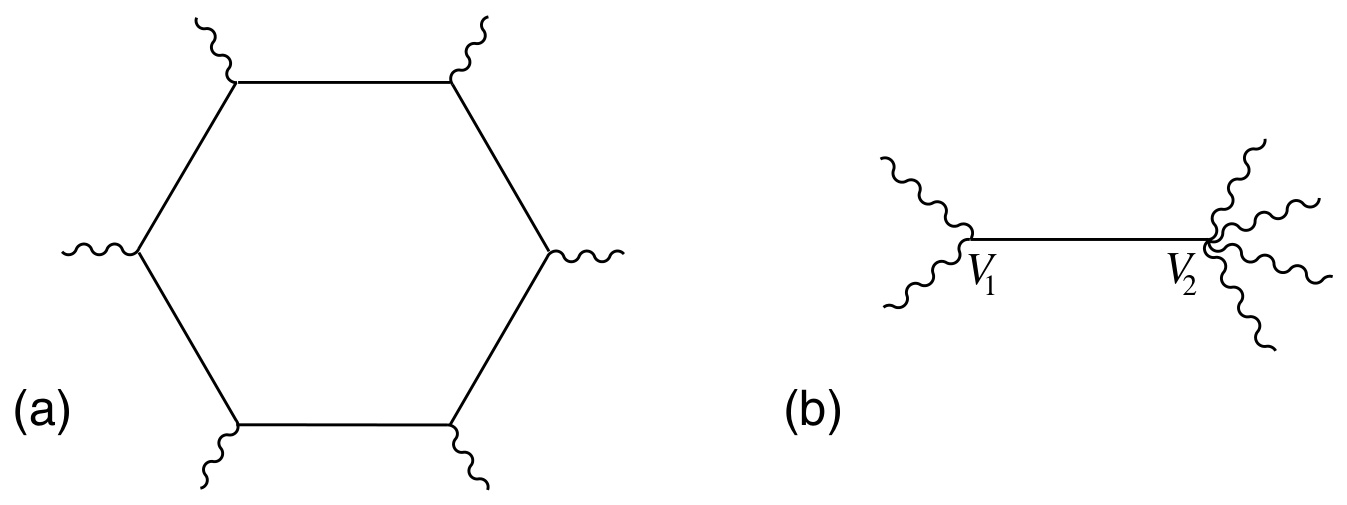
\includegraphics[width=0.7\textwidth]{figure/Fig12.1.jpg}
	\caption{Graphs contributing to the spacetime anomalies. One of the six external lines is a current and the others are gauge or gravitational fields: (a) 1-loop hexagon graph; (b) canceling tree graph from the exchange of the $B_{\mu\nu}$ field.}
	\label{fig:12.1}
\end{figure}

\begin{equation}
	\delta Z[A] = -\pi \int \dif^{2}z\:\lambda^{a}(z,\bar{z})
	\Bigl[\hat{k}_{L}\partial_{z}A_{\bar{z}}^{a}(z,\bar{z})+\hat{k}_{R}\partial_{\bar{z}}A_{z}^{a}(z,\bar{z})\Bigr]\:.
	\label{12.2.3}
\end{equation}
\begin{tcolorbox}[breakable]
	\begin{remark}
		\textbf{Conventions.} The notes do not define $Z[A]$ or the normalization of $\lambda^{a}$, so we fix them here.
		\begin{itemize}
			\item[(i)] Currents are normalized as in \eqref{11.5.1} and \eqref{11.5.7} with $d^{ab}=\delta^{ab}$ (the basis chosen below \eqref{11.5.13}): $j^{a}(z)j^{b}(0)\sim\hat k_{L}\delta^{ab}z^{-2}+\mi c^{abc}j^{c}(0)z^{-1}$, and likewise for $\tilde\jmath^{a}(\bar z)$ with $\hat k_{R}$. Since $d^{ab}=\delta^{ab}$, index positions on $c^{abc}$ do not matter, and $c^{abc}$ is totally antisymmetric.
			\item[(ii)] $Z[A]\equiv\bigl\langle\exp\bigl(\mi\int\dif^{2}z\,[A^{a}_{\bar z}j^{a}+A^{a}_{z}\tilde\jmath^{a}]\bigr)\bigr\rangle$, with $Z[0]=1$, and ``$\delta Z$'' means $\delta\ln Z$ (the same thing at leading order). Here $A_{\bar z}=A^{\text{can}}_{\bar z}/2\pi$, where $A^{\text{can}}$ couples to the canonically normalized Noether current $j/2\pi$ (Polchinski's normalization of CFT currents; this is the $2\pi$ of \eqref{12.3.33}). The factor $\mi$ is our choice: it is the Euclidean coupling of a real gauge field to Hermitian currents.
			\item[(iii)] $\delta A^{\text{can}}=D\lambda^{\text{can}}$ with $D=\partial-\mi[A^{\text{can}},\cdot\,]$, i.e.\ $\delta A^{\text{can},a}=\partial\lambda^{\text{can},a}+c^{abc}A^{\text{can},b}\lambda^{\text{can},c}$, as in \eqref{12.1.37} and \eqref{12.3.32}.
			\item[(iv)] The parameter in \eqref{12.2.3} is $\lambda\equiv\lambda^{\text{can}}/\pi$, so that $\delta A^{a}_{\bar z}=\frac12\partial_{\bar z}\lambda^{a}+\pi c^{abc}A^{b}_{\bar z}\lambda^{c}$. This is a choice: it is the normalization for which the coefficient is the printed $-\pi$. With $\lambda=\lambda^{\text{can}}/2\pi$ the same computation gives $-2\pi$.
			\item[(v)] $\dif^{2}z=2\dif\sigma^{1}\dif\sigma^{2}$ and $\partial_{\bar z}z^{-1}=2\pi\delta^{2}(z,\bar z)$, from \eqref{2.1.24}.
		\end{itemize}
		Write $\langle\mathcal O\rangle_{A}$ for the normalized expectation value in the presence of the background. The holomorphic half gives
		\begin{align*}
			\delta\ln Z&=\mi\int\dif^{2}z\,\delta A^{a}_{\bar z}\,\langle j^{a}(z)\rangle_{A}\\
			&\eqs{1} -\frac{\mi}{2}\int\dif^{2}z\,\lambda^{a}\langle\bar\partial j^{a}(z)\rangle_{A}+\mi\pi c^{abc}\int\dif^{2}z\,A^{b}_{\bar z}\lambda^{c}\langle j^{a}\rangle_{A},\\
			\langle\bar\partial j^{a}(z)\rangle_{A}&\eqs{2} \mi\int\dif^{2}w\,A^{b}_{\bar w}(w)\,\partial_{\bar z}\Bigl[\frac{\hat k_{L}\delta^{ab}}{(z-w)^{2}}+\frac{\mi c^{abc}\langle j^{c}(w)\rangle_{A}}{z-w}\Bigr]\\
			&\eqs{3} -2\pi\mi\hat k_{L}\,\partial_{z}A^{a}_{\bar z}(z)-2\pi c^{abc}A^{b}_{\bar z}(z)\langle j^{c}(z)\rangle_{A},\\
			\delta\ln Z&\eqs{4} -\pi\hat k_{L}\int\dif^{2}z\,\lambda^{a}\partial_{z}A^{a}_{\bar z}
			+\mi\pi\int\dif^{2}z\,\bigl(c^{abc}\lambda^{a}A^{b}_{\bar z}\langle j^{c}\rangle_{A}+c^{abc}A^{b}_{\bar z}\lambda^{c}\langle j^{a}\rangle_{A}\bigr)\\
			&\eqs{5} -\pi\hat k_{L}\int\dif^{2}z\,\lambda^{a}\partial_{z}A^{a}_{\bar z} .
		\end{align*}
		At (1), the $\frac12\partial_{\bar z}\lambda$ term was integrated by parts. At (2), $\bar\partial j^{a}=0$ away from other currents, so inside the correlator $\partial_{\bar z}$ acts only on the singular terms of the OPE \eqref{11.5.1} of $j^{a}(z)$ with the currents in the exponent. For currents that OPE is exact, so the result holds to all orders in $A$. At (3), $\partial_{\bar z}(z-w)^{-2}=-\partial_{z}\partial_{\bar z}(z-w)^{-1}=-2\pi\partial_{z}\delta^{2}(z-w)$ and $\partial_{\bar z}(z-w)^{-1}=2\pi\delta^{2}(z-w)$, after which the $w$ integral is trivial. At (4), $-\frac{\mi}{2}(-2\pi\mi)=-\pi$. At (5), relabeling $a\leftrightarrow c$ in the second term and using $c^{cba}=-c^{abc}$ shows that the two $c^{abc}$ terms cancel. This cancellation is the classical gauge invariance, and it is what ties the $\pi c^{abc}$ in (iv) to the factor $\mi$ in (ii). The antiholomorphic half is identical, with $\partial_{z}\bar z^{-1}=2\pi\delta^{2}$, and gives $-\pi\hat k_{R}\int\lambda^{a}\partial_{\bar z}A^{a}_{z}$. Together these give \eqref{12.2.3}.

		\emph{Counterterm and descent.} Split \eqref{12.2.3} as
		\begin{align*}
			&-\pi\int\lambda^{a}\bigl(\hat k_{L}\partial_{z}A^{a}_{\bar z}+\hat k_{R}\partial_{\bar z}A^{a}_{z}\bigr)\\
			&\quad=-\frac{\pi}{2}(\hat k_{L}-\hat k_{R})\int\lambda^{a}\bigl(\partial_{z}A^{a}_{\bar z}-\partial_{\bar z}A^{a}_{z}\bigr)
			-\frac{\pi}{2}(\hat k_{L}+\hat k_{R})\int\lambda^{a}\bigl(\partial_{z}A^{a}_{\bar z}+\partial_{\bar z}A^{a}_{z}\bigr),\\
			&\delta\int\dif^{2}z\,A^{a}_{z}A^{a}_{\bar z}\eqs{6} -\frac12\int\dif^{2}z\,\lambda^{a}\bigl(\partial_{z}A^{a}_{\bar z}+\partial_{\bar z}A^{a}_{z}\bigr) .
		\end{align*}
		At (6), the $c^{abc}$ terms cancel because $A^{a}_{z}A^{a}_{\bar z}$ is adjoint invariant. So the local counterterm $\ln Z\to\ln Z-\pi(\hat k_{L}+\hat k_{R})\int A^{a}_{z}A^{a}_{\bar z}$ removes the second piece. The first piece, $\propto(\hat k_{L}-\hat k_{R})$, cannot be removed and is the genuine anomaly: it vanishes for vector-like theories. It is the consistent anomaly obtained by descent from $I_{4}\propto\operatorname{Tr}(F\wedge F)$: by the box after \eqref{12.1.37}, $\dif\omega_{3}=\operatorname{Tr}(F\wedge F)$ and $\delta\omega_{3}=\dif\operatorname{Tr}(\lambda\dif A)$, so $\omega^{1}_{2}=\operatorname{Tr}(\lambda\dif A)$, and $\dif A=(\partial_{z}A_{\bar z}-\partial_{\bar z}A_{z})\dif z\wedge\dif\bar z$ reproduces the combination $\lambda^{a}(\partial_{z}A^{a}_{\bar z}-\partial_{\bar z}A^{a}_{z})$. Descent also explains why the anomaly is exactly linear in $A$. In the heterotic application below, $\hat k_{L}=1$ (the $\lambda^{A}$) and $\hat k_{R}=0$.
	\end{remark}
\end{tcolorbox}

\section{Superspace and Superfields}

To construct superstring perturbation theory, it is more beneficial to first give superconformal symmetry a more geometric interpretation. To do this, we need a \textit{supermanifold}, which is a world-sheet with one ordinary complex coordinate $z$ and one anticommuting complex coordinate $\theta$, where
\begin{equation}
	\theta^{2}=\bar{\theta}^{2} = \{\theta,\bar{\theta}\} = 0 \:. \label{12.3.1}
\end{equation}
Due to anticommutativity, the Taylor expansion of any function of $\theta$ and $\bar{\theta}$ is truncated. Thus, we can view any function on the supermanifold as a set of ordinary functions appearing in the Taylor expansion. However, just as the operator "$\int\theta$" has many properties of an ordinary integral and thus we call it an integration, the behavior of $\theta$ is also very much like a coordinate, so it is useful to view this as a manifold with both ordinary and anticommuting coordinates.

We can view ordinary conformal transformations this way. Under a generalized transformation $z^{\prime}(z,\bar{z})$ of world-sheet coordinates, the transformation of derivatives is
\begin{equation}
	\partial_{z} = \frac{\partial z^{\prime}}{\partial z} \partial_{z^{\prime}}
	+\frac{\partial \bar{z}^{\prime}}{\partial z} \partial_{\bar{z}^{\prime}} \:.\label{12.3.2}
\end{equation}
Conformal transformations are those transformations that turn $\partial_{z}$ into a multiple of itself.

Define \textit{superderivatives},
\begin{equation}
	D_{\theta} = \partial_{\theta} + \theta \partial_{z}\:, \qquad \quad 
	D_{\bar{\theta}} = \partial_{\bar{\theta}}+ \bar{\theta}\partial_{\bar{z}} \:, \label{12.3.3}
\end{equation}
which have the following properties
\begin{equation}
	D_{\theta}^{2} = \partial_{z}\:, \qquad D_{\bar{\theta}}^{2} = \partial_{\bar{z}}\:,\qquad
	\{D_{\theta},D_{\bar{\theta}}\} = 0 \:. \label{12.3.4}
\end{equation}
\begin{tcolorbox}[breakable]
	Note that
	\begin{align*}
		(\partial_{\theta}+\theta\partial_{z})^{2}f =\partial_{\theta}\Bigl(\theta \partial_{z}f\Bigr)
		+\theta \partial_{z}\partial_{\theta} f = \partial_{z}f - \theta \partial_{\theta}\partial_{z}f
		+\theta \partial_{z}\partial_{\theta} f \:,
	\end{align*}
	The absence of a quadratic term in the first equal sign is due to the anticommutativity of $\theta$, and the negative sign of the second term in the second equal sign is for the same reason.
	\begin{align*}
		\{D_{\theta},D_{\bar{\theta}}\} &=\partial_{\theta}\partial_{\bar{\theta}}f+ \theta\bar{\theta}\partial_{z}\partial_{\bar{z}}f+\theta\partial_{\bar{\theta}}\partial_{z}f
		-\bar{\theta}\partial_{\theta}\partial_{\bar{z}}f \\
		&\quad +\partial_{\bar{\theta}}\partial_{\theta}f+ \bar{\theta}\theta\partial_{z}\partial_{\bar{z}}f
		+\bar{\theta}\partial_{\theta}\partial_{\bar{z}}f -\theta\partial_{\bar{\theta}}\partial_{z}f =0
	\end{align*}
\end{tcolorbox}
\noindent Superconformal transformations $z^{\prime}(z,\theta)$, $\theta^{\prime}(z,\theta)$ are transformations that turn $D_{\theta}$ into a multiple of itself. From
\begin{equation}
	D_{\theta} = D_{\theta} \theta^{\prime} \partial_{\theta^{\prime}}
	+D_{\theta}z^{\prime}\partial_{z^{\prime}} + D_{\theta}\bar{\theta}^{\prime}\partial_{\bar{\theta}^{\prime}}
	+D_{\theta}\bar{z}^{\prime}\partial_{\bar{z}^{\prime}} \:, \label{12.3.5}
\end{equation}
it follows that superconformal transformations satisfy
\begin{equation}
	D_{\theta}\bar{\theta}^{\prime}=D_{\theta}\bar{z}^{\prime}=0\:, \qquad \quad
	D_{\theta}z^{\prime} = \theta^{\prime}D_{\theta}\theta^{\prime} \:, \label{12.3.6}
\end{equation}
hence
\begin{equation}
	D_{\theta}= (D_{\theta}\theta^{\prime})D_{\theta^{\prime}} \:. \label{12.3.7}
\end{equation}
\begin{tcolorbox}[breakable]
	First prove \eqref{12.3.5}
	\begin{align*}
		D_{\theta} = \frac{\partial}{\partial \theta} + \theta \frac{\partial}{\partial z}
		&= \frac{\partial \theta^{\prime}}{\partial \theta} \frac{\partial}{\partial \theta^{\prime}}
		+ \frac{\partial z^{\prime}}{\partial \theta} \frac{\partial}{\partial z^{\prime}} 
		+\frac{\partial \bar{\theta}^{\prime}}{\partial \theta} \frac{\partial}{\partial \bar{\theta^{\prime}}}
		+ \frac{\partial \bar{z}^{\prime}}{\partial \theta} \frac{\partial}{\partial \bar{z}^{\prime}} \\
		&\quad+ \theta \frac{\partial \theta^{\prime}}{\partial z}\frac{\partial}{\partial \theta^{\prime}}
		+\theta \frac{\partial z^{\prime}}{\partial z}\frac{\partial}{\partial z^{\prime}}
		+ \theta \frac{\partial \bar{\theta}^{\prime}}{\partial z}\frac{\partial}{\partial \bar{\theta}^{\prime}}
		+\theta \frac{\partial \bar{z}^{\prime}}{\partial z}\frac{\partial}{\partial \bar{z}^{\prime}} \\
		&=D_{\theta} \theta^{\prime} \partial_{\theta^{\prime}}
		+D_{\theta}z^{\prime}\partial_{z^{\prime}} + D_{\theta}\bar{\theta}^{\prime}\partial_{\bar{\theta}^{\prime}}
		+D_{\theta}\bar{z}^{\prime}\partial_{\bar{z}^{\prime}} ,
	\end{align*}
	Using \eqref{12.3.6} on \eqref{12.3.5} yields
	\begin{align*}
		D_{\theta} \theta^{\prime} \partial_{\theta^{\prime}}
		+D_{\theta}z^{\prime}\partial_{z^{\prime}} + D_{\theta}\bar{\theta}^{\prime}\partial_{\bar{\theta}^{\prime}}
		+D_{\theta}\bar{z}^{\prime}\partial_{\bar{z}^{\prime}}
		=D_{\theta} \theta^{\prime} \partial_{\theta^{\prime}}
		+\theta^{\prime}D_{\theta}\theta^{\prime}\partial_{z^{\prime}}=(D_{\theta}\theta^{\prime})D_{\theta^{\prime}}\:.
	\end{align*}
\end{tcolorbox}
\noindent Using $D_{\theta}^{2}=\partial_{z}$ allows concluding that
\begin{equation}
	\partial_{\bar{z}}z^{\prime}=\partial_{\bar{\theta}}z^{\prime}=\partial_{\bar{z}}\theta^{\prime}
	=\partial_{\bar{\theta}}\theta^{\prime} =0  \label{12.3.8}
\end{equation}
\begin{tcolorbox}[breakable]
	The conjugate of \eqref{12.3.6} states $D_{\bar\theta}\theta'=D_{\bar\theta}z'=0$. Applying $D_{\bar\theta}$ once more and using $D_{\bar\theta}^{2}=\partial_{\bar z}$ from \eqref{12.3.4},
	\begin{align*}
		\partial_{\bar z}z'\eqs{1} D_{\bar\theta}\bigl(D_{\bar\theta}z'\bigr)=0,\qquad
		\partial_{\bar\theta}z'\eqs{2} D_{\bar\theta}z'-\bar\theta\,\partial_{\bar z}z'=0 ,
	\end{align*}
	and identically for $\theta'$. At (1), $D_{\bar\theta}^{2}=\partial_{\bar z}$. At (2), the definition \eqref{12.3.3} of $D_{\bar\theta}$ was used together with the result of (1). So $z'$ and $\theta'$ depend on neither $\bar z$ nor $\bar\theta$.
\end{tcolorbox}
\noindent and its conjugate relations. From this, we can solve for superconformal transformations and represent them using a holomorphic commuting function $f(z)$ and a holomorphic anticommuting function $g(z)$,
\begin{subequations}
	\begin{align}
		z^{\prime}(z,\theta) &= f(z)+\theta g(z)h(z) \:, \qquad 
		\theta^{\prime}(z,\theta)=g(z)+\theta h(z) \:, \label{12.3.9a} \\
		h(z) &= \pm\Bigl[\partial_{z}f(z)+g(z)\partial_{z}g(z)\Bigr]^{1/2} \label{12.3.9b}
	\end{align} \label{12.3.9}
\end{subequations}
The infinitesimal form is
\begin{equation}
	\delta z= \epsilon[v(z)-\mi\theta\eta(z)] \:, \qquad 
	\delta \theta =\epsilon[-\mi\eta(z)+\tfrac{1}{2}\theta\partial v(z)]  \label{12.3.10}
\end{equation}
where $\epsilon$ and $v$ commute, and $\eta$ anticommutes. They satisfy the superconformal algebra \eqref{10.1.11}.
\begin{tcolorbox}[breakable]
	First, $z^{\prime}$ must be in the form shown in \eqref{12.3.9a}. We can write $\theta^{\prime}$ as
	\[
	\theta^{\prime}(z,\theta)=g^{\prime}(z)+\theta h^{\prime}(z)
	\]
	Then use \eqref{12.3.6}
	\begin{align*}
		D_{\theta}z^{\prime} &= (\partial_{\theta}+\theta\partial_{z})(f+\theta gh)= gh+\theta \partial_{z} f \\
		\theta^{\prime}D_{\theta}\theta^{\prime} &=(g^{\prime}+\theta h^{\prime})(\partial_{\theta}+\theta\partial_{z})
		(g^{\prime}+\theta h^{\prime})
		=(g^{\prime}+\theta h^{\prime})(h^{\prime}+\theta \partial_{z} g^{\prime}) \\
		&=g^{\prime}h^{\prime}+\theta (h^{\prime}h^{\prime}-g^{\prime}\partial_{z} g^{\prime})
	\end{align*}
	From this it is not difficult to obtain
	\[
	g^{\prime}h^{\prime}=gh \:, \qquad h^{\prime}h^{\prime}=g^{\prime}\partial_{z} g^{\prime}+\partial f 
	\]
	Choosing $g^{\prime}=g$ and $h^{\prime}=h$ is completely possible, thus obtaining \eqref{12.3.9}.
	
	For the infinitesimal form, it is easy to see that $f\sim O(z)$, $h\sim O(1)$ and $g\sim O(\epsilon)$, which means \eqref{12.3.9b} must take the positive sign; therefore, we might as well take $f=z+\epsilon v(z)$ and $g=-\mi\epsilon\eta(z)$, then \eqref{12.3.9b} yields $h$:
	\[
	h=1+\tfrac{1}{2}\epsilon\partial_{z}v(z) \:.
	\]
\end{tcolorbox}

Analogous to the transformation of conformal tensors, the transformation of a \textit{tensor superfield} with weight $(h,\tilde{h})$ is
\begin{equation}
	(D_{\theta}\theta^{\prime})^{2h}(D_{\bar{\theta}}\bar{\theta}^{\prime})^{2\tilde{h}}
	\bm{\phi}^{\prime}(\bm{z}^{\prime},\bar{\bm{z}}^{\prime}) = \bm{\phi}(\bm{z},\bar{\bm{z}}) \:, \label{12.3.11}
\end{equation}
where $\bm{z}$ represents $(z,\theta)$. In an infinitesimal superconformal transformation $\delta \theta=\epsilon\eta(z)$,
\begin{equation}
	\delta\bm{\phi}(\bm{z},\bar{\bm{z}})=-\epsilon
	\Bigl[2h\theta\partial\eta(z)+\eta(z)Q_{\theta}+2\tilde{h}\bar{\theta}\bar{\partial}\bar{\eta}(\bar{z})
	+\bar{\eta}(\bar{z})Q_{\bar{\theta}}\Bigr]\bm{\phi}(\bm{z},\bar{\bm{z}}) \:, \label{12.3.12}
\end{equation}
where $Q_{\theta}=\partial_{\theta}-\theta\partial_{z}$ and $Q_{\bar{\theta}}=\partial_{\bar{\theta}}-\bar{\theta}\partial_{\bar{z}}$.
\begin{tcolorbox}[breakable]
	$\delta\theta = \epsilon\eta(z)$ corresponds to taking $g(z)=\epsilon\eta(z),\,h(z)=1$ and $f(z)=z$ in \eqref{12.3.9a}, then $z^{\prime}=z+\epsilon\theta\eta(z)$, so $\delta \bm{\phi}$ is (considering only the holomorphic part for simplicity):
	\begin{align*}
		\delta\bm{\phi}&= \bm{\phi}^{\prime}(\bm{z})-\bm{\phi}(\bm{z}) = \bm{\phi}^{\prime}(z^{\prime}-\epsilon\theta\eta,\theta^{\prime}-\epsilon\eta)-\bm{\phi}(z,\theta) \\
		&=\bm{\phi}^{\prime}(z^{\prime},\theta^{\prime})
		-\epsilon\theta\eta\partial_{z^{\prime}}\bm{\phi}^{\prime}(z^{\prime},\theta^{\prime})
		-\epsilon\eta\partial_{\theta^{\prime}}\bm{\phi}^{\prime}(z^{\prime},\theta^{\prime}) -\bm{\phi}(z,\theta)\\
		&=(D_{\theta}\theta^{\prime})^{-2h}\bm{\phi}(\bm{z})-\bm{\phi}(\bm{z})
		-\epsilon\eta Q_{\theta}\Bigl((D_{\theta}\theta^{\prime})^{-2h}\bm{\phi}(\bm{z})\Bigr) \\
		&= -2h\epsilon\theta(\partial_{z}\eta) \bm{\phi} -\epsilon\eta Q_{\theta}\bm{\phi}
	\end{align*}
	Note that we used $(D_{\theta}\theta^{\prime})^{-2h}=(1+\epsilon\theta\partial\eta)^{-2h}=1-2h\epsilon\theta\partial\eta$, and in the third equal sign we used the anticommutativity of $\theta$ and $\eta$, thus obtaining $Q_{\theta}$ rather than $D_{\theta}$.
\end{tcolorbox}
Expanding into a Taylor series in $\theta$—focusing only on the holomorphic part for simplicity—we have
\begin{equation}
	\bm{\phi}(\bm{z}) = \mathcal{O}(z)+\theta \varPsi(z) \:. \label{12.3.13}
\end{equation}
Then the infinitesimal transformation \eqref{12.3.12} is
\begin{equation}
	\delta \mathcal{O} = -\epsilon\eta\varPsi\:, \qquad 
	\delta \varPsi=-\epsilon[2h\partial\eta \mathcal{O}+\eta\partial\mathcal{O}] \:. \label{12.3.14}
\end{equation}
Written as OPE coefficients \eqref{10.3.4}, this is
\begin{subequations}
	\begin{align}
		G_{{-}1/2}\cdot \mathcal{O} &= \varPsi\:, \qquad G_{r}\cdot \mathcal{O}=0\:, \quad r\geq \tfrac{1}{2} \:,\label{12.3.15a} \\ 
		G_{{-}1/2}\cdot \varPsi &= \partial\mathcal{O}\:, \qquad G_{1/2}\cdot \varPsi = 2h\mathcal{O}\:,
		\qquad G_{r}\cdot\varPsi=0\:,\quad r\geq \tfrac{3}{2} \:. \label{12.3.15b}
	\end{align}\label{12.3.15}
\end{subequations}
\begin{tcolorbox}[breakable]
	\begin{remark}
		Derivation of \eqref{12.3.14} and \eqref{12.3.15}. Insert $\bm\phi=\mathcal O+\theta\varPsi$ into \eqref{12.3.12} (holomorphic part; $\epsilon$ commuting, $\eta$ anticommuting):
		\begin{align*}
			\delta\mathcal O+\theta\,\delta\varPsi
			&=-\epsilon\Bigl[2h\theta\partial\eta+\eta\bigl(\partial_{\theta}-\theta\partial\bigr)\Bigr](\mathcal O+\theta\varPsi)
			\eqs{1} -\epsilon\Bigl[2h\theta\partial\eta\,\mathcal O+\eta\varPsi-\eta\theta\,\partial\mathcal O\Bigr]\\
			&\eqs{2} -\epsilon\eta\varPsi+\theta\Bigl(-\epsilon\bigl[2h\partial\eta\,\mathcal O+\eta\partial\mathcal O\bigr]\Bigr) .
		\end{align*}
		At (1), $\theta\partial\eta\,\theta\varPsi=-\theta\theta\,\partial\eta\varPsi=0$, $\partial_{\theta}(\theta\varPsi)=\varPsi$ and $\theta\partial(\theta\varPsi)=0$. At (2), $-\eta\theta=\theta\eta$. Reading off the $\theta^{0}$ and $\theta^{1}$ terms gives \eqref{12.3.14}.

		To get \eqref{12.3.15}, compare with the Ward identity \eqref{10.3.4}, $\delta\mathscr A=-\epsilon\sum_{n}\frac{1}{n!}\partial^{n}\eta\,G_{n-1/2}\cdot\mathscr A$, identifying its $\eta$ with the one in \eqref{12.3.12}. Since $\eta(z)$ is arbitrary, the coefficients of $\eta,\partial\eta,\partial^{2}\eta,\dots$ at the operator position must match separately:
		\begin{align*}
			\delta\mathcal O=-\epsilon\bigl[\eta\,G_{-1/2}+\partial\eta\,G_{1/2}+\cdots\bigr]\cdot\mathcal O\;&\overset{!}{=}\;-\epsilon\eta\varPsi ,\\
			\delta\varPsi=-\epsilon\bigl[\eta\,G_{-1/2}+\partial\eta\,G_{1/2}+\cdots\bigr]\cdot\varPsi\;&\overset{!}{=}\;-\epsilon\bigl[\eta\,\partial\mathcal O+\partial\eta\,2h\mathcal O\bigr] ,
		\end{align*}
		so that
		\begin{align*}
			G_{-1/2}\cdot\mathcal O=\varPsi,\quad G_{r\ge1/2}\cdot\mathcal O=0,\qquad
			G_{-1/2}\cdot\varPsi=\partial\mathcal O,\quad G_{1/2}\cdot\varPsi=2h\mathcal O,\quad G_{r\ge3/2}\cdot\varPsi=0 .
		\end{align*}
	\end{remark}
\end{tcolorbox}
Whether through the use of the NS algebra or by considering pure conformal transformations $\delta z=\epsilon v(z)$, it can be found that $\mathcal{O}$ is a tensor with weight $h$, while $\varPsi$ is a tensor with weight $h+\tfrac{1}{2}$, so both are annihilated by all Virasoro lowering generators. The lowest component $\mathcal{O}$ of this tensor superfield is a \textit{superconformal primary field}, which is annihilated by all lowering generators of the NS algebra.

Contrasting rigid translation, now rigid world-sheet supersymmetric translation is $\delta\theta ={-}\mi\epsilon\eta$, $\delta z={-}\mi\epsilon\theta\eta$. The Ward identity for $T_{F}$ gives the corresponding generator
\begin{equation}
	G_{{-}1/2}\cdot \sim -\mi Q_{\theta} = -\mi(\partial_{\theta}-\theta\partial_{z}) \label{12.3.16}
\end{equation}
\begin{tcolorbox}[breakable]
	\begin{remark}
		\textbf{Conventions, and the inconsistency.} The text uses two incompatible identifications of the parameter $\eta$ with a superspace transformation. \eqref{12.3.12}--\eqref{12.3.15} take $\delta\theta=+\epsilon\eta$, while \eqref{12.3.10} and \eqref{12.3.16} take $\delta\theta=-\mi\epsilon\eta$, so their $\eta$'s differ by a factor $\mi$. Neither matches the free-field OPE: with \eqref{12.3.19}, $G_{-1/2}\cdot X=-\mi\psi=-\varPsi$, whereas \eqref{12.3.15} says $+\varPsi$, and $-\mi Q_{\theta}\bm X|_{\theta=0}=-\mi\varPsi=+\psi$. In addition, \eqref{10.3.4} is printed with $-\epsilon$, while the Ward identity actually used to derive \eqref{10.1.10a}--\eqref{10.1.10c} (the box before it) gives $+\mi\epsilon$. We fix one consistent set:
		\begin{itemize}
			\item[(i)] The Ward identity of the box before \eqref{10.1.10a} (Polchinski's \eqref{2.3.11} form): $\delta\mathscr A(z)=\mi\epsilon\operatorname{Res}_{w\to z}\eta(w)T_{F}(w)\mathscr A(z)$. With $T_{F}(w)\mathscr A(z)=\sum_{r}(w-z)^{-r-3/2}G_{r}\cdot\mathscr A(z)$ this is $\delta\mathscr A=\mi\epsilon\sum_{n}\frac{1}{n!}\partial^{n}\eta\,G_{n-1/2}\cdot\mathscr A$, i.e.\ \eqref{10.3.4} with $-\epsilon\to\mi\epsilon$.
			\item[(ii)] $T_{F}=\mi(2/\alpha')^{1/2}\psi\cdot\partial X$ at $\alpha'=2$, the superfield \eqref{12.3.19}, and $\psi\psi\sim\eta/z$, $XX\sim-\ln\lvert z\rvert^{2}$.
			\item[(iii)] $G_{r}$ is fermionic: $G_{r}\cdot(\theta\mathscr A)=-\theta\,G_{r}\cdot\mathscr A$.
		\end{itemize}
		The OPE coefficients $G_{r}\cdot$ are fixed by $T_{F}$ alone and do not depend on (i). Only the map from $\eta$ to $(\delta z,\delta\theta)$ does.

		\emph{The generator on the free superfield.} From the OPEs in the box before \eqref{10.1.10a}, at $\alpha'=2$,
		\begin{gather*}
			T_{F}(w)X^{\mu}(z)\sim\frac{-\mi\psi^{\mu}(z)}{w-z},\quad T_{F}(w)\psi^{\mu}(z)\sim\frac{\mi\partial X^{\mu}(z)}{w-z}\\
			\Longrightarrow\quad G_{-1/2}\cdot X^{\mu}=-\mi\psi^{\mu},\quad G_{-1/2}\cdot\psi^{\mu}=\mi\partial X^{\mu},
		\end{gather*}
		\begin{align*}
			G_{-1/2}\cdot\bm X^{\mu}=G_{-1/2}\cdot X^{\mu}+\mi\,G_{-1/2}\cdot(\theta\psi^{\mu})
			&\eqs{1} -\mi\psi^{\mu}-\mi\theta\,(\mi\partial X^{\mu})=-\mi\psi^{\mu}+\theta\partial X^{\mu}\\
			&\eqs{2} -Q_{\theta}\bm X^{\mu} .
		\end{align*}
		At (1), (iii) was used. At (2), $Q_{\theta}\bm X=\partial_{\theta}\bm X-\theta\partial\bm X=\mi\psi-\theta\partial X$ (holomorphic part). As a check, $G_{-1/2}\cdot(G_{-1/2}\cdot X)=-\mi\,G_{-1/2}\cdot\psi=\partial X=L_{-1}\cdot X$, as required by $\{G_{-1/2},G_{-1/2}\}=2L_{-1}$.

		\emph{The transformation generated by $\eta$.} By (i), $\delta X=\mi\epsilon\eta(-\mi\psi)=\epsilon\eta\psi$ and $\delta\psi=\mi\epsilon\eta(\mi\partial X)=-\epsilon\eta\partial X$, which is \eqref{10.1.10a}--\eqref{10.1.10c} at $\alpha'=2$. The superspace map $\delta\theta=a\epsilon\eta$, $\delta z=a\epsilon\theta\eta$ gives, by the box after \eqref{12.3.12} with $\eta\to a\eta$ (constant $\eta$, $h=0$),
		\begin{align*}
			\delta\bm X=-a\epsilon\eta\,Q_{\theta}\bm X
			\quad\Longrightarrow\quad \delta X=-\mi a\,\epsilon\eta\psi
			\quad\eqs{3}\quad a=\mi .
		\end{align*}
		At (3), this was matched to $\delta X=\epsilon\eta\psi$. So $\eta$ generates $\delta\theta=\mi\epsilon\eta$, $\delta z=\mi\epsilon\theta\eta$, which is \eqref{12.3.10} with $\eta\to-\eta$.

		\emph{General tensor superfield.} For weight $h$, the transformation with $\delta\theta=\mi\epsilon\eta(z)$ is \eqref{12.3.12} with $\eta\to\mi\eta$, so by the box after \eqref{12.3.15}, $\delta\mathcal O=-\mi\epsilon\eta\varPsi$ and $\delta\varPsi=-\mi\epsilon(2h\partial\eta\,\mathcal O+\eta\partial\mathcal O)$. Matching with (i) coefficient by coefficient in $\eta,\partial\eta,\dots$:
		\begin{align*}
			G_{-1/2}\cdot\mathcal O=-\varPsi,\quad G_{r\ge1/2}\cdot\mathcal O=0,\\
			G_{-1/2}\cdot\varPsi=-\partial\mathcal O,\quad G_{1/2}\cdot\varPsi=-2h\,\mathcal O,\quad G_{r\ge3/2}\cdot\varPsi=0,
		\end{align*}
		and for Grassmann-even $\mathcal O$,
		\begin{align*}
			G_{-1/2}\cdot\bm\phi=G_{-1/2}\cdot\mathcal O-\theta\,G_{-1/2}\cdot\varPsi\eqs{4} -\varPsi+\theta\partial\mathcal O=-Q_{\theta}\bm\phi .
		\end{align*}
		At (4), the component results above were used. This agrees with the free-field result ($h=0$, $\mathcal O=X$, $\varPsi=\mi\psi$).

		So in one consistent convention, \eqref{12.3.16} reads $G_{-1/2}\cdot\sim-Q_{\theta}$, and \eqref{12.3.15} holds with $\varPsi\to-\varPsi$ (i.e.\ for the superfield written as $\mathcal O-\theta\varPsi$). The structural statement, that $G_{-1/2}\cdot$ acts on superfields as $Q_{\theta}$ up to a constant phase and thus generates the rigid translation $\theta\to\theta+{}$const, $z\to z+\theta\,{}$const, holds in any convention. The phase is what (i)--(iii) fix. Acting twice gives $L_{-1}$, as checked on $X$ above.
	\end{remark}
\end{tcolorbox}
This generalizes $L_{{-}1}\cdot \sim \partial_{z}$ obtained in CFT.

\subsection*{Actions and backgrounds}

The super-Jacobian matrix of transformation \eqref{12.3.9} is
\begin{equation}
	\dif z^{\prime}\,\dif\theta^{\prime} = \dif z\,\dif\theta\,D_{\theta}\theta^{\prime}\:. \label{12.3.17}
\end{equation}
\begin{tcolorbox}[breakable]
	\begin{remark}
		Derivation of \eqref{12.3.17}. The Jacobian of a change of variables $(z,\theta)\to(z',\theta')$ is the Berezinian (superdeterminant)
		\[
		\dif z'\,\dif\theta'=\dif z\,\dif\theta\;\frac{A-BD^{-1}C}{D},\qquad
		A=\partial_{z}z',\quad B=z'\overleftarrow{\partial_{\theta}},\quad C=\partial_{z}\theta',\quad D=\partial_{\theta}\theta' .
		\]
		The fermionic derivative in the odd entry $B$ must act from the right; with it, $\int\dif z'\dif\theta'\,F=\int\dif z\,\dif\theta\,\mathrm{Ber}\,F$. This can be checked directly on $z'=z+\theta g$, $\theta'=\theta+g$, for which both sides give $\mathrm{Ber}=1+gg'+\theta g'$. For \eqref{12.3.9}, $z'=f+\theta gh=f-gh\,\theta$, so
		\begin{align*}
			A&=\partial f+\theta\,\partial(gh),\qquad B=-gh,\qquad C=\partial g+\theta\,\partial h,\qquad D=h,\\
			A-BD^{-1}C&\eqs{1} \partial f+\theta(\partial g\,h+g\,\partial h)+g\,\partial g+g\theta\,\partial h
			\eqs{2} \partial f+g\,\partial g+\theta\,h\,\partial g
			\eqs{3} h^{2}+\theta\,h\,\partial g ,\\
			\frac{A-BD^{-1}C}{D}&=h+\theta\,\partial g
			\eqs{4} D_{\theta}\theta' .
		\end{align*}
		At (1), $-BD^{-1}C=g(\partial g+\theta\partial h)$. At (2), $g\theta=-\theta g$, so the two $\theta g\,\partial h$ terms cancel. At (3), $h^{2}=\partial f+g\partial g$ from \eqref{12.3.9b}. At (4), $D_{\theta}\theta'=(\partial_{\theta}+\theta\partial)(g+\theta h)=h+\theta\partial g$.
	\end{remark}
\end{tcolorbox}
To construct a superconformally invariant action, the Lagrangian density must be a tensor superfield with weight $(\tfrac{1}{2},\tfrac{1}{2})$. The product of two tensor superfields is also a tensor superfield, whose weight is the sum of the original two weights, $(h,\tilde{h})=(h_{1},\tilde{h}_{1})+(h_{2},\tilde{h}_{2})$. Additionally, the superderivative $D_{\theta}$ turns a $(0,\tilde{h})$ tensor superfield into a $(\tfrac{1}{2},\tilde{h})$ tensor superfield, while $D_{\bar{\theta}}$ turns an $(h,0)$ tensor superfield into an $(h,\tfrac{1}{2})$ tensor superfield.

We can construct an invariant action from $d$ tensors $\bm{X}^{\mu}(\bm{z},\bar{\bm{z}})$ with weight $(0,0)$:
\begin{equation}
	S= \frac{1}{4\pi} \int \dif^{2}z\,\dif^{2}\theta\: D_{\bar{\theta}}\bm{X}^{\mu}D_{\theta}\bm{X}_{\mu}\:.\label{12.3.18} 
\end{equation}
The Taylor expansion of $\bm{X}^{\mu}$ with respect to $\theta$ is
\begin{equation}
	\bm{X}^{\mu}(\bm{z},\bar{\bm{z}})=X^{\mu}+\mi\theta \psi^{\mu}+\mi\bar{\theta}\tilde{\psi}^{\mu}
	+\theta\bar{\theta}F^{\mu} \:. \label{12.3.19}
\end{equation}
where $\alpha^{\prime}=2$ is set, and can be restored via $X^{\mu}\to X^{\mu}(2/\alpha^{\prime})^{1/2}$. Integration over $\dif^{2}\theta=\dif\theta\,\dif\bar{\theta}$ in the action picks out the coefficient of $\bar{\theta}\theta$
\begin{equation}
	S=\frac{1}{4\pi}\int\dif^{2}z\:\Bigl(\partial_{\bar{z}}X^{\mu}\partial_{z}X_{\mu}+\psi^{\mu}\partial_{\bar{z}}psi_{\mu}+\tilde{\psi}^{\mu}\partial_{z}\tilde{\psi}_{\mu}+F^{\mu}F_{\mu}\Bigr) \:. \label{12.3.20}
\end{equation}
The field $F^{\mu}$ is an auxiliary field, completely determined by the equations of motion—here being zero. The remainder of the action is identical to the previous \eqref{10.1.5}.

Many previous results can be recast in superfield form; the equation of motion is
\begin{equation}
	D_{\theta}D_{\bar{\theta}}\bm{X}^{\mu}(\bm{z},\bar{\bm{z}})=0\:. \label{12.3.21}
\end{equation}
\begin{tcolorbox}[breakable]
	\begin{remark}
		Derivation of \eqref{12.3.20} and \eqref{12.3.21}. Acting on \eqref{12.3.19} with \eqref{12.3.3},
		\begin{align*}
			D_{\theta}\bm X^{\mu}&\eqs{1} \mi\psi^{\mu}+\bar\theta F^{\mu}+\theta\partial X^{\mu}+\mi\theta\bar\theta\,\partial\tilde\psi^{\mu},\\
			D_{\bar\theta}\bm X^{\mu}&\eqs{1} \mi\tilde\psi^{\mu}-\theta F^{\mu}+\bar\theta\bar\partial X^{\mu}+\mi\bar\theta\theta\,\bar\partial\psi^{\mu} .
		\end{align*}
		At (1), $\partial_{\theta}(\theta\bar\theta F)=\bar\theta F$ and $\partial_{\bar\theta}(\theta\bar\theta F)=-\theta F$, and the $\theta\partial$ ($\bar\theta\bar\partial$) term keeps only the $\theta$-independent ($\bar\theta$-independent) components. In the product $D_{\bar\theta}\bm X^{\mu}D_{\theta}\bm X_{\mu}$, the $\bar\theta\theta$ component receives four contributions:
		\begin{align*}
			(\mi\tilde\psi^{\mu})(\mi\theta\bar\theta\,\partial\tilde\psi_{\mu})&\eqs{2}\bar\theta\theta\,\tilde\psi^{\mu}\partial\tilde\psi_{\mu},\qquad
			(-\theta F^{\mu})(\bar\theta F_{\mu})\eqs{2}\bar\theta\theta\,F^{\mu}F_{\mu},\\
			(\bar\theta\bar\partial X^{\mu})(\theta\partial X_{\mu})&=\bar\theta\theta\,\bar\partial X^{\mu}\partial X_{\mu},\qquad
			(\mi\bar\theta\theta\,\bar\partial\psi^{\mu})(\mi\psi_{\mu})\eqs{3}\bar\theta\theta\,\psi^{\mu}\bar\partial\psi_{\mu} .
		\end{align*}
		At (2), $\theta\bar\theta=-\bar\theta\theta$. At (3), $-\bar\partial\psi^{\mu}\psi_{\mu}=\psi_{\mu}\bar\partial\psi^{\mu}$ by anticommutation. Every other product has an unpaired $\theta$ or $\bar\theta$, or contains $\theta^{2}$ or $\bar\theta^{2}$. Since $\int\dif\theta\,\dif\bar\theta\,\bar\theta\theta=1$, this gives \eqref{12.3.20}, and the $F^{\mu}$ equation of motion is $F^{\mu}=0$. Similarly,
		\begin{align*}
			D_{\theta}D_{\bar\theta}\bm X^{\mu}
			\eqs{4} -F^{\mu}-\mi\bar\theta\,\bar\partial\psi^{\mu}+\mi\theta\,\partial\tilde\psi^{\mu}+\theta\bar\theta\,\partial\bar\partial X^{\mu}=0 .
		\end{align*}
		At (4), $\partial_{\theta}(\bar\theta\theta)=-\bar\theta$. The four components are $F^{\mu}=0$, $\bar\partial\psi^{\mu}=0$, $\partial\tilde\psi^{\mu}=0$ and $\partial\bar\partial X^{\mu}=0$, all the component equations of motion at once.
	\end{remark}
\end{tcolorbox}
For OPEs, invariance under translation and rigid supersymmetric transformations tells us it can only be a function of $z_{1}-z_{2}-\theta_{1}\theta_{2}$, $\theta_{1}-\theta_{2}$, and their conjugates. In this case,
\begin{equation}
	\bm{X}^{\mu}(\bm{z}_{1},\bar{\bm{z}}_{1})\bm{X}^{\nu}(\bm{z}_{2},\bar{\bm{z}}_{2})\sim
	-\eta^{\mu\nu}\ln\lvert z_{1}-z_{2}-\theta_{1}\theta_{2}\rvert^{2} \:, \label{12.3.22}
\end{equation}
which can be proven by expansion into component fields.
\begin{tcolorbox}[breakable]
	Translation and rigid supersymmetry transformations of $\theta$ tell us $z$ and $\theta$ can only appear as $z_{1}-z_{2}$ and $\theta_{1}-\theta_{2}$. Then rigid supersymmetry transformation of $z$ yields
	\[
	\delta_{\text{super}}(z_{1}-z_{2}) = -\mi\epsilon\theta_{1}\eta+\mi\epsilon\theta_{2}\eta \:,
	\]
	while rigid supersymmetry transformation of $\theta_{1}\theta_{2}$ yields
	\[
	\delta_{\text{super}}(\theta_{1}\theta_{2})= \delta(\theta_{1})\theta_{2}+\theta_{1}\delta(\theta_{2})
	=\theta_{1}(-\mi\epsilon\eta)+(-\mi\epsilon\eta)\theta_{2}
	\]
	The two cancel exactly.
\end{tcolorbox}
\begin{tcolorbox}[breakable]
	Component check of \eqref{12.3.22}. Expand in the nilpotent $\theta_{1}\theta_{2}$:
	\begin{align*}
		-\eta^{\mu\nu}\ln\lvert z_{12}-\theta_{1}\theta_{2}\rvert^{2}
		&\eqs{1} -\eta^{\mu\nu}\ln\lvert z_{12}\rvert^{2}+\eta^{\mu\nu}\frac{\theta_{1}\theta_{2}}{z_{12}}+\eta^{\mu\nu}\frac{\bar\theta_{1}\bar\theta_{2}}{\bar z_{12}} ,\\
		\bm X^{\mu}(\bm z_{1})\bm X^{\nu}(\bm z_{2})
		&\eqs{2} X^{\mu}X^{\nu}+\theta_{1}\theta_{2}\,\psi^{\mu}(z_{1})\psi^{\nu}(z_{2})+\bar\theta_{1}\bar\theta_{2}\,\tilde\psi^{\mu}(\bar z_{1})\tilde\psi^{\nu}(\bar z_{2})+\cdots .
	\end{align*}
	At (1), $\ln(z_{12}-\theta_{1}\theta_{2})=\ln z_{12}-\theta_{1}\theta_{2}/z_{12}$ exactly, since $(\theta_{1}\theta_{2})^{2}=0$. At (2), $(\mi\theta_{1}\psi^{\mu})(\mi\theta_{2}\psi^{\nu})=-\theta_{1}\psi^{\mu}\theta_{2}\psi^{\nu}=\theta_{1}\theta_{2}\psi^{\mu}\psi^{\nu}$; the dots are mixed $\psi\tilde\psi$ terms, which have no singular OPE, and terms with $F$, whose OPE is a contact term only. Matching coefficients reproduces $X^{\mu}X^{\nu}\sim-\eta^{\mu\nu}\ln\lvert z_{12}\rvert^{2}$, $\psi^{\mu}\psi^{\nu}\sim\eta^{\mu\nu}/z_{12}$ and $\tilde\psi^{\mu}\tilde\psi^{\nu}\sim\eta^{\mu\nu}/\bar z_{12}$, the free OPEs at $\alpha'=2$.
\end{tcolorbox}
The superconformal ghost action is built with tensor superfields $B$ and $C$ with weights $(\lambda-\frac{1}{2})$ and $(1-\lambda,0)$, respectively,
\begin{equation}
	S_{BC}=\frac{1}{2\pi}\int \dif^{2}z\,\dif^{2}\theta\: B D_{\bar{\theta}}C \:. \label{12.3.23}
\end{equation}
The equations of motion are
\begin{equation}
	D_{\bar{\theta}}B= D_{\bar{\theta}}C=0 \:. \label{12.3.24}
\end{equation}
Applying $D_{\bar{\theta}}$ to this equation yields $\partial_{\bar{z}}B=\partial_{\bar{z}}C=0$, and hence $\partial_{\bar{\theta}}B=\partial_{\bar{\theta}}C=0$. Thus the equations of motion yield
\begin{equation}
	B(\bm{z})=\beta(z)+\theta b(z) \:, \qquad C(\bm{z})=c(z)+\theta\gamma(z)\:. \label{12.3.25}
\end{equation}
This is identical to theory \eqref{10.1.17}. The OPE is
\begin{equation}
	B(\bm{z}_{1})C(\bm{z}_{2})\sim \frac{\theta_{1}-\theta_{2}}{z_{1}-z_{2}-\theta_{1}\theta_{2}}
	=\frac{\theta_{1}-\theta_{2}}{z_{1}-z_{2}} \:. \label{12.3.26}
\end{equation}
\begin{tcolorbox}[breakable]
	Components of \eqref{12.3.26}. The second equality holds because $(\theta_{1}-\theta_{2})\theta_{1}\theta_{2}=0$, so $\frac{\theta_{12}}{z_{12}-\theta_{1}\theta_{2}}=\frac{\theta_{12}}{z_{12}}\bigl(1+\frac{\theta_{1}\theta_{2}}{z_{12}}\bigr)=\frac{\theta_{12}}{z_{12}}$. With \eqref{12.3.25},
	\begin{align*}
		B(\bm z_{1})C(\bm z_{2})
		\eqs{1} \beta(z_{1})c(z_{2})+\theta_{1}\,b(z_{1})c(z_{2})+\theta_{2}\,\beta(z_{1})\gamma(z_{2})-\theta_{1}\theta_{2}\,b(z_{1})\gamma(z_{2})
		\sim\frac{\theta_{1}}{z_{12}}-\frac{\theta_{2}}{z_{12}} .
	\end{align*}
	At (1), $\beta$ is commuting and $b$ anticommutes with $\theta_{2}$. Matching powers of $\theta$ gives $b(z_{1})c(z_{2})\sim1/z_{12}$ and $\beta(z_{1})\gamma(z_{2})\sim-1/z_{12}$, which are the $bc$ and $\beta\gamma$ OPEs of chapter 10, with no singular $\beta c$ and $b\gamma$ terms.
\end{tcolorbox}
The superfield form makes writing the non-linear $\sigma$ model action very simple
\begin{align}
	S &= \frac{1}{4\pi}\int\dif^{2}z\,\dif^{2}\theta\:[G_{\mu\nu}(\bm{X})+B_{\mu\nu}(\bm{X})]
	D_{\bar{\theta}}\bm{X}^{\nu}D_{\theta}\bm{X}^{\mu} \nonumber \\ 
	&=\frac{1}{4\pi}\int \dif^{2}z\:\Bigl\{[G_{\mu\nu}(X)+B_{\mu\nu}(X)]\partial_{z}X^{\mu}\partial_{\bar{z}}X^{\nu}
	\nonumber \\
	&\qquad \quad+G_{\mu\nu}(X)(\psi^{\mu}\mathscr{D}_{\bar{z}}\psi^{\nu}+\tilde{\psi}^{\mu}\mathscr{D}_{z}\tilde{\psi}^{\nu})+\tfrac{1}{2}R_{\mu\nu\rho\sigma}(X)\psi^{\mu}\psi^{\nu}\tilde{\psi}^{\rho}\tilde{\psi}^{\sigma}\Bigr\}\:,
	\label{12.3.27}
\end{align}
auxiliary fields are eliminated in the second equal sign. The Christoffel connection and antisymmetric tensor field strength form the covariant derivative
\begin{subequations}
	\begin{align}
		\mathscr{D}_{\bar{z}}\psi^{\nu} &= \partial_{\bar{z}}\psi^{\nu}
		+\Bigl[\Gamma\indices{^\nu_\rho_\sigma}(X)+\tfrac{1}{2}H\indices{^\nu_\rho_\sigma}(X)\Bigr]\partial_{\bar{z}}X^{\rho}\psi^{\sigma} \:, \label{12.3.28a} \\
		\mathscr{D}_{z}\tilde{\psi}^{\nu} &= \partial_{z}\tilde{\psi}^{\nu} 
		+\Bigl[\Gamma\indices{^\nu_\rho_\sigma}(X)-\tfrac{1}{2}H\indices{^\nu_\rho_\sigma}(X)\Bigr]
		\partial_{z}X^{\rho}\tilde{\psi}^{\sigma} \:. \label{12.3.28b}
	\end{align} \label{12.3.28}
\end{subequations}
\begin{tcolorbox}[breakable]
	\begin{remark}
		Derivation of \eqref{12.3.27} and \eqref{12.3.28}. Write $E_{\mu\nu}=G_{\mu\nu}+B_{\mu\nu}$ and expand $E_{\mu\nu}(\bm X)$ around $X$ with $\bm X-X=\mi\theta\psi+\mi\bar\theta\tilde\psi+\theta\bar\theta F$:
		\begin{align*}
			E_{\mu\nu}(\bm X)&\eqs{1} E_{\mu\nu}+\mi\theta E_{\mu\nu,\rho}\psi^{\rho}+\mi\bar\theta E_{\mu\nu,\rho}\tilde\psi^{\rho}
			-\bar\theta\theta\bigl(E_{\mu\nu,\rho}F^{\rho}+E_{\mu\nu,\rho\sigma}\psi^{\rho}\tilde\psi^{\sigma}\bigr) .
		\end{align*}
		At (1), the quadratic term is $\frac12E_{,\rho\sigma}\bigl[(\mi\theta\psi^{\rho})(\mi\bar\theta\tilde\psi^{\sigma})+(\mi\bar\theta\tilde\psi^{\rho})(\mi\theta\psi^{\sigma})\bigr]=\theta\bar\theta\,E_{,\rho\sigma}\psi^{\rho}\tilde\psi^{\sigma}$, and $\theta\bar\theta=-\bar\theta\theta$. Using the components of $D_{\theta}\bm X$, $D_{\bar\theta}\bm X$ from the box after \eqref{12.3.21}, write $P^{\nu\mu}=D_{\bar\theta}\bm X^{\nu}D_{\theta}\bm X^{\mu}=P_{0}+\theta P_{\theta}+\bar\theta P_{\bar\theta}+\bar\theta\theta P_{\bar\theta\theta}$ with
		\begin{align*}
			P_{0}&=-\tilde\psi^{\nu}\psi^{\mu},\qquad
			P_{\theta}=-\mi F^{\nu}\psi^{\mu}-\mi\tilde\psi^{\nu}\partial X^{\mu},\qquad
			P_{\bar\theta}=\mi\bar\partial X^{\nu}\psi^{\mu}-\mi\tilde\psi^{\nu}F^{\mu},\\
			P_{\bar\theta\theta}&=\tilde\psi^{\nu}\partial\tilde\psi^{\mu}+F^{\nu}F^{\mu}+\bar\partial X^{\nu}\partial X^{\mu}-\bar\partial\psi^{\nu}\psi^{\mu} .
		\end{align*}
		The $\bar\theta\theta$ component of $E_{\mu\nu}(\bm X)P^{\nu\mu}$, picked out by $\int\dif^{2}\theta$, is then
		\begin{align*}
			\mathcal L&\eqs{2} E_{\mu\nu}P_{\bar\theta\theta}+E_{\bar\theta\theta}P_{0}+E_{\theta}P_{\bar\theta}-E_{\bar\theta}P_{\theta}\\
			&= E_{\mu\nu}\bigl(\partial X^{\mu}\bar\partial X^{\nu}+\psi^{\mu}\bar\partial\psi^{\nu}+\tilde\psi^{\nu}\partial\tilde\psi^{\mu}+F^{\nu}F^{\mu}\bigr)
			+E_{\mu\nu,\rho\sigma}\psi^{\rho}\tilde\psi^{\sigma}\tilde\psi^{\nu}\psi^{\mu}\\
			&\quad -E_{\mu\nu,\rho}\psi^{\rho}\psi^{\mu}\bar\partial X^{\nu}-E_{\mu\nu,\rho}\tilde\psi^{\rho}\tilde\psi^{\nu}\partial X^{\mu}+F^{\lambda}J_{\lambda} ,\\
			J_{\lambda}&\eqs{3} \bigl(E_{\mu\nu,\lambda}-E_{\lambda\nu,\mu}-E_{\mu\lambda,\nu}\bigr)\tilde\psi^{\nu}\psi^{\mu}
			\eqs{4} \bigl(-2\Gamma_{\lambda\mu\nu}+H_{\lambda\mu\nu}\bigr)\tilde\psi^{\nu}\psi^{\mu} .
		\end{align*}
		At (2), $(\theta E_{\theta})(\bar\theta P_{\bar\theta})=\bar\theta\theta E_{\theta}P_{\bar\theta}$ and $(\bar\theta E_{\bar\theta})(\theta P_{\theta})=-\bar\theta\theta E_{\bar\theta}P_{\theta}$, since $E_{\theta}$ and $E_{\bar\theta}$ are odd. At (3), the three terms linear in $F$ were collected and all fermion pairs ordered as $\tilde\psi\psi$. At (4), $\Gamma_{\lambda\mu\nu}=\frac12(G_{\lambda\mu,\nu}+G_{\lambda\nu,\mu}-G_{\mu\nu,\lambda})$ and $H_{\lambda\mu\nu}=\partial_{\lambda}B_{\mu\nu}+\partial_{\mu}B_{\nu\lambda}+\partial_{\nu}B_{\lambda\mu}$.

		\emph{Connection terms.} In the fermion kinetic terms the $B$ part is not zero but a total derivative plus a connection term:
		\[
		B_{\mu\nu}\psi^{\mu}\bar\partial\psi^{\nu}\simeq-\tfrac12B_{\mu\nu,\rho}\bar\partial X^{\rho}\psi^{\mu}\psi^{\nu},\qquad
		B_{\mu\nu}\tilde\psi^{\nu}\partial\tilde\psi^{\mu}\simeq\tfrac12B_{\mu\nu,\rho}\partial X^{\rho}\tilde\psi^{\mu}\tilde\psi^{\nu},
		\]
		obtained from $\bar\partial(B_{\mu\nu}\psi^{\mu}\psi^{\nu})$ and $\partial(B_{\mu\nu}\tilde\psi^{\nu}\tilde\psi^{\mu})$. Relabel so that every term reads $(\cdots)_{\mu\rho\sigma}\psi^{\mu}\psi^{\sigma}\bar\partial X^{\rho}$ and antisymmetrize in $\mu\sigma$:
		\begin{align*}
			&-E_{\mu\nu,\rho}\psi^{\rho}\psi^{\mu}\bar\partial X^{\nu}-\tfrac12B_{\mu\sigma,\rho}\psi^{\mu}\psi^{\sigma}\bar\partial X^{\rho}\\
			&\eqs{5} \Bigl[\tfrac12\bigl(G_{\mu\rho,\sigma}-G_{\sigma\rho,\mu}\bigr)-\tfrac12\bigl(B_{\sigma\rho,\mu}+B_{\rho\mu,\sigma}+B_{\mu\sigma,\rho}\bigr)\Bigr]\psi^{\mu}\psi^{\sigma}\bar\partial X^{\rho}\\
			&\eqs{6} \Bigl(\Gamma_{\mu\rho\sigma}+\tfrac12H_{\mu\rho\sigma}\Bigr)\psi^{\mu}\psi^{\sigma}\bar\partial X^{\rho}\\
			&=G_{\mu\nu}\psi^{\mu}\Bigl(\Gamma\indices{^\nu_\rho_\sigma}+\tfrac12H\indices{^\nu_\rho_\sigma}\Bigr)\bar\partial X^{\rho}\psi^{\sigma} .
		\end{align*}
		At (5), only the part antisymmetric in $\mu\sigma$ survives against $\psi^{\mu}\psi^{\sigma}$. At (6), $\Gamma_{\mu\rho\sigma}-\Gamma_{\sigma\rho\mu}=G_{\mu\rho,\sigma}-G_{\sigma\rho,\mu}$ (the symmetric part of $\Gamma_{\mu\rho\sigma}$ in $\mu\sigma$ drops), and the $B$ bracket is $H_{\mu\sigma\rho}=-H_{\mu\rho\sigma}$. Together with $G_{\mu\nu}\psi^{\mu}\bar\partial\psi^{\nu}$ this is $G_{\mu\nu}\psi^{\mu}\mathscr D_{\bar z}\psi^{\nu}$ with \eqref{12.3.28a}. The $\tilde\psi$ terms go the same way, except that in $-E_{\mu\nu,\rho}\tilde\psi^{\rho}\tilde\psi^{\nu}\partial X^{\mu}$ the fermions carry the \emph{second} index of $E_{\mu\nu}$. Transposing $E$ is $B\to-B$, which gives $\Gamma-\frac12H$ in \eqref{12.3.28b}.

		\emph{Auxiliary field and curvature.} The $F$ terms are $G_{\mu\nu}F^{\mu}F^{\nu}+F^{\lambda}J_{\lambda}$, so $F^{\kappa}=-\frac12G^{\kappa\lambda}J_{\lambda}$, and eliminating $F$ leaves $-\frac14G^{\kappa\lambda}J_{\kappa}J_{\lambda}$. For $H=0$ (the case displayed in \eqref{12.3.27}) the result is covariant, so it may be evaluated in Riemann normal coordinates at a point, where $G_{\mu\nu,\rho}=0$. There $J=0$, and the connection terms vanish, leaving
		\begin{align*}
			G_{\mu\nu,\rho\sigma}\psi^{\rho}\tilde\psi^{\sigma}\tilde\psi^{\nu}\psi^{\mu}
			&\eqs{7} G_{bd,ac}\,\psi^{a}\psi^{b}\tilde\psi^{c}\tilde\psi^{d}\\
			&\eqs{8} -\tfrac13\bigl(R_{badc}+R_{bcda}\bigr)\psi^{a}\psi^{b}\tilde\psi^{c}\tilde\psi^{d}
			\eqs{9} -\tfrac12R_{abcd}\,\psi^{a}\psi^{b}\tilde\psi^{c}\tilde\psi^{d} .
		\end{align*}
		At (7), $\psi^{\mu}$ was moved past two $\tilde\psi$'s and the indices renamed. At (8), the normal-coordinate expansion $G_{\mu\nu}(x_{0}+Y)=G_{\mu\nu}-\frac13R_{\mu\lambda\nu\kappa}Y^{\lambda}Y^{\kappa}+O(Y^{3})$ was used. At (9), $R_{badc}=R_{abcd}$. Antisymmetrizing $R_{bcda}=R_{dabc}$ in $ab$ and using the cyclic identity $R_{dabc}+R_{dbca}+R_{dcab}=0$ gives $\frac12R_{abcd}$. In this curvature convention the coefficient is $-\frac12$; the $+\frac12$ printed in \eqref{12.3.27} corresponds to the opposite sign convention for $R_{\mu\nu\rho\sigma}$. For $H\neq0$ the $J^{2}$ term adds further four-fermion terms quadratic in $H$.
	\end{remark}
\end{tcolorbox}
This describes general NS--NS backgrounds in both Type II superstring theories. R--R backgrounds are difficult to describe within this framework because superconformal transformations produce branch cuts on the operators. The dilaton does not appear in the flat world-sheet action, but it does appear in superconformal generators.

All the above can be applied to heterotic strings, in which case only $\bar{\theta}$ is used and $\theta$ is not. Now superfields are needed:
\begin{subequations}
	\begin{align}
		\bm{X}^{\mu} &= X^{\mu}+\mi\bar{\theta}\tilde{\psi}^{\mu} \:, \label{12.3.29a} \\
		\bm{\lambda}^{A} &= \lambda^{A} + \bar{\theta}G^{A} \:. \label{12.3.29b} 
	\end{align} \label{12.3.29}
\end{subequations}
$G^{A}$ is an auxiliary field. The non-linear $\sigma$ model is
\begin{align}
	S&= \frac{1}{4\pi} \int \dif^{2}z\,\dif\bar{\theta}\:\Bigl\{[G_{\mu\nu}(\bm{X})+B_{\mu\nu}(\bm{X})]
	\partial_{z}\bm{X}^{\mu}D_{\bar{\theta}}\bm{X}^{\nu} 
	- \bm{\lambda}^{A}\mathscr{D}_{\bar{\theta}}\bm{\lambda}^{A} \Bigr\} \nonumber \\
	&=\frac{1}{4\pi} \int \dif^{2}z\:\Bigl\{ [G_{\mu\nu}(X)+B_{\mu\nu}X]\partial_{z}X^{\mu}\partial_{\bar{z}}X^{\nu}
	+G_{\mu\nu}(X)\tilde{\psi}^{\mu}\mathscr{D}_{z}\tilde{\psi}^{\nu} \nonumber \\
	&\phantom{=\frac{1}{4\pi} \int \dif^{2}z\:\Bigl\{ [G_{\mu\nu}}+\lambda^{A}\mathscr{D}_{\bar{z}}\lambda^{A}
	+\tfrac{\mi}{2}F_{\rho\sigma}^{AB}(X)\lambda^{A}\lambda^{B}\tilde{\psi}^{\rho}\tilde{\psi}^{\sigma}\Bigr\}\:,
	\label{12.3.30}
\end{align}
where $\mathscr{D}_{z}\tilde{\psi}^{\nu}$ is as above, and
\begin{subequations}
	\begin{align}
		\mathscr{D}_{\bar{\theta}}\bm{\lambda}^{A}&=D_{\bar{\theta}}\bm{\lambda}^{A}
		-\mi A_{\mu}^{AB}(\bm{X})D_{\bar{\theta}}\bm{X}^{\mu}\bm{\lambda}^{B} \:, \label{12.3.31a} \\
		\mathscr{D}_{\bar{z}}\lambda^{A} &= \partial_{\bar{z}}\lambda^{A} 
		- \mi A_{\mu}^{AB}(X)\partial_{\bar{z}}X^{\mu}\lambda^{B} \:. \label{12.3.31b}
	\end{align} \label{12.3.31}
\end{subequations}
\begin{tcolorbox}[breakable]
	\begin{remark}
		Derivation of the gauge sector of \eqref{12.3.30}. The $\bm X$ sector works as in the box after \eqref{12.3.28}, with only $\bar\theta$ present, and gives the $G\partial X\bar\partial X$ and $G\tilde\psi\mathscr D_{z}\tilde\psi$ terms. For the current algebra fermions, $A_{\mu}(\bm X)=A_{\mu}+\mi\bar\theta A_{\mu,\rho}\tilde\psi^{\rho}$ and $D_{\bar\theta}\bm X^{\mu}=\mi\tilde\psi^{\mu}+\bar\theta\bar\partial X^{\mu}$, and $A_{\mu}^{AB}=-A_{\mu}^{BA}$ in the vector representation. Then
		\begin{align*}
			A_{\mu}(\bm X)D_{\bar\theta}\bm X^{\mu}&\eqs{1} \mi A_{\mu}\tilde\psi^{\mu}+\bar\theta\,m,\qquad m\equiv A_{\mu}\bar\partial X^{\mu}-A_{\mu,\rho}\tilde\psi^{\rho}\tilde\psi^{\mu},\\
			\mathscr D_{\bar\theta}\bm\lambda^{A}&\eqs{2} \bigl(G^{A}+A_{\mu}^{AB}\tilde\psi^{\mu}\lambda^{B}\bigr)
			+\bar\theta\bigl(\bar\partial\lambda^{A}-A_{\mu}^{AB}\tilde\psi^{\mu}G^{B}-\mi m^{AB}\lambda^{B}\bigr)\equiv a^{A}+\bar\theta\,b^{A},\\
			-\bm\lambda^{A}\mathscr D_{\bar\theta}\bm\lambda^{A}\Big|_{\bar\theta}&\eqs{3} \lambda^{A}b^{A}-G^{A}a^{A}
			=\lambda^{A}\bar\partial\lambda^{A}-\mi\lambda^{A}m^{AB}\lambda^{B}-G^{A}G^{A}-2G^{A}A_{\mu}^{AB}\tilde\psi^{\mu}\lambda^{B} .
		\end{align*}
		At (1), $(\mi\bar\theta A_{\mu,\rho}\tilde\psi^{\rho})(\mi\tilde\psi^{\mu})=-\bar\theta A_{\mu,\rho}\tilde\psi^{\rho}\tilde\psi^{\mu}$. At (2), $D_{\bar\theta}\bm\lambda=G+\bar\theta\bar\partial\lambda$, and in $-\mi(\mi A\tilde\psi+\bar\theta m)(\lambda+\bar\theta G)$ the $\bar\theta$ was moved past the odd $\tilde\psi$. At (3), $-(\lambda+\bar\theta G)(a+\bar\theta b)=-\lambda a+\bar\theta(\lambda b-Ga)$, and the two terms linear in $G$ are equal after using the antisymmetry of $A^{AB}$ and anticommuting $\lambda^{A}$ past $\tilde\psi^{\mu}$. The auxiliary field equation is $G^{A}=-A^{AB}_{\mu}\tilde\psi^{\mu}\lambda^{B}$, i.e.\ $a^{A}=0$, and substituting back gives
		\begin{align*}
			-G^{A}G^{A}-2G^{A}A^{AB}_{\mu}\tilde\psi^{\mu}\lambda^{B}
			&=A^{AB}_{\mu}\tilde\psi^{\mu}\lambda^{B}A^{AC}_{\nu}\tilde\psi^{\nu}\lambda^{C}
			\\&\eqs{4} (A_{\mu}A_{\nu})^{BC}\tilde\psi^{\mu}\tilde\psi^{\nu}\lambda^{B}\lambda^{C}
			=\tfrac12[A_{\mu},A_{\nu}]^{AB}\tilde\psi^{\mu}\tilde\psi^{\nu}\lambda^{A}\lambda^{B},\\
			-\mi\lambda^{A}m^{AB}\lambda^{B}
			&\eqs{5} -\mi A^{AB}_{\mu}\bar\partial X^{\mu}\lambda^{A}\lambda^{B}\\
			&\qquad+\tfrac{\mi}{2}\bigl(\partial_{\mu}A_{\nu}-\partial_{\nu}A_{\mu}\bigr)^{AB}\tilde\psi^{\mu}\tilde\psi^{\nu}\lambda^{A}\lambda^{B} .
		\end{align*}
		At (4), $\tilde\psi^{\mu}\lambda^{B}\tilde\psi^{\nu}\lambda^{C}=-\tilde\psi^{\mu}\tilde\psi^{\nu}\lambda^{B}\lambda^{C}$ and $A^{AB}_{\mu}A^{AC}_{\nu}=-(A_{\mu}A_{\nu})^{BC}$. At (5), $\tilde\psi^{\rho}\tilde\psi^{\mu}$ antisymmetrizes $A_{\mu,\rho}$. Collecting terms,
		\begin{align*}
		&\lambda^{A}\bigl(\bar\partial\lambda^{A}-\mi A^{AB}_{\mu}\bar\partial X^{\mu}\lambda^{B}\bigr)
		+\tfrac{\mi}{2}\bigl(\partial_{\mu}A_{\nu}-\partial_{\nu}A_{\mu}-\mi[A_{\mu},A_{\nu}]\bigr)^{AB}\lambda^{A}\lambda^{B}\tilde\psi^{\mu}\tilde\psi^{\nu}\\
		&\qquad=\lambda^{A}\mathscr D_{\bar z}\lambda^{A}+\tfrac{\mi}{2}F^{AB}_{\mu\nu}\lambda^{A}\lambda^{B}\tilde\psi^{\mu}\tilde\psi^{\nu},
		\end{align*}
		which is the gauge part of \eqref{12.3.30} with \eqref{12.3.31b}. The commutator from eliminating the auxiliary field is exactly what makes the abelian curl into the non-abelian field strength $F=\dif A-\mi A\wedge A$.
	\end{remark}
\end{tcolorbox}
It is noteworthy that the modified gauge transformation of the 2-form potential, which plays an important role in canceling spacetime anomalies, has a simple origin in the form of a world-sheet anomaly.
The spacetime gauge transformations
\begin{equation}
	\delta A_{\mu}^{AB}= D_{\mu}\chi^{AB} \:, \qquad \delta\lambda^{A} = \mi \chi^{AB}\lambda^{B} \label{12.3.32}
\end{equation}
leave the classical action invariant. However, it acts only on left-moving world-sheet fermions and therefore has an anomaly in the world-sheet path integral. We can use result \eqref{12.2.3}, setting $\hat{k}_{L}=1$, $\hat{k}_{R}=0$, and
\begin{equation}
	A_{\bar{z}}^{AB}(z,\bar{z})=\frac{1}{2\pi}A_{\mu}^{AB}(X)\partial_{\bar{z}}X^{\mu} \:, \label{12.3.33}
\end{equation}
the factor $2\pi$ corrects the non-standard normalization of Noether currents in CFT. Then adding the counterterm,
\begin{equation}
	\delta Z[A] = \frac{1}{8\pi}\int \dif^{2}z\: \operatorname{Tr}_{\mathrm{v}}[\chi(X)F_{\mu\nu}(X)]\partial_{z}X^{\mu}\partial_{\bar{z}}X^{\nu} \:. \label{12.3.34}
\end{equation}
\begin{tcolorbox}[breakable]
	\begin{remark}
		\textbf{Conventions.} We use those of the box after \eqref{12.2.3}, together with the world-sheet action \eqref{12.3.30}--\eqref{12.3.31} exactly as printed (at $\alpha'=2$). $A_{\mu}=A^{a}_{\mu}t^{a}$ and $\chi=\chi^{a}t^{a}$ with Hermitian vector-representation generators $[t^{a},t^{b}]=\mi c^{abc}t^{c}$, normalized by the current algebra as $\operatorname{Tr}_{\mathrm v}(t^{a}t^{b})=2\delta^{ab}$ (the statement below \eqref{11.5.13} that the $SO(n)$ inner product is half the vector trace). The counterterm is the one of the previous box, pulled back with $A_{z}=\frac{1}{2\pi}A_{\mu}\partial X^{\mu}$ and $A_{\bar z}=\frac{1}{2\pi}A_{\mu}\bar\partial X^{\mu}$.

		First the current and its coupling. Let $J^{a}=\frac12\lambda^{A}t^{a}_{AB}\lambda^{B}$. Then
		\begin{align*}
			J^{a}(z)J^{b}(0)&\eqs{1} \frac14t^{a}_{AB}t^{b}_{CD}\,\frac{\delta^{AD}\delta^{BC}-\delta^{AC}\delta^{BD}}{z^{2}}+\frac{\frac12\lambda^{T}[t^{a},t^{b}]\lambda}{z}\\
			&\eqs{2} \frac{\frac12\operatorname{Tr}_{\mathrm v}(t^{a}t^{b})}{z^{2}}+\frac{\mi c^{abc}J^{c}(0)}{z}=\frac{\delta^{ab}}{z^{2}}+\frac{\mi c^{abc}J^{c}(0)}{z},\\
			\me^{-S}&\supset\exp\Bigl[\frac{\mi}{4\pi}\int\dif^{2}z\,A^{AB}_{\mu}\bar\partial X^{\mu}\lambda^{A}\lambda^{B}\Bigr]
			\eqs{3} \exp\Bigl[\frac{\mi}{2\pi}\int\dif^{2}z\,A^{a}_{\mu}\bar\partial X^{\mu}J^{a}\Bigr]\\
			&=\exp\Bigl[\mi\int\dif^{2}z\,A^{a}_{\bar z}J^{a}\Bigr],\\
			A^{a}_{\bar z}&=\frac{1}{2\pi}A^{a}_{\mu}\bar\partial X^{\mu} .
		\end{align*}
		At (1), $\lambda^{A}(z)\lambda^{B}(0)\sim\delta^{AB}/z$ from the $\frac{1}{4\pi}\lambda\bar\partial\lambda$ kinetic term was used, with the fermion signs of the two double contractions. The single contractions combine into the bilinear of the commutator. At (2), $t^{a}_{AB}t^{b}_{AB}=-\operatorname{Tr}_{\mathrm v}(t^{a}t^{b})$ because the $t^{a}$ are antisymmetric. So $J^{a}$ is a level $\hat k_{L}=1$ current with the same structure constants as the $t^{a}$. At (3), the $-\mi A^{AB}\bar\partial X\lambda^{B}$ term of $\mathscr D_{\bar z}\lambda^{A}$ in $\frac{1}{4\pi}\lambda^{A}\mathscr D_{\bar z}\lambda^{A}$ was used, together with $A^{AB}\lambda^{A}\lambda^{B}=2A^{a}J^{a}$. This is \eqref{12.3.33} in the form (ii) of the previous box. Its $A^{\text{can}}_{\bar z}=A_{\mu}\bar\partial X^{\mu}$ transforms under \eqref{12.3.32} as $D_{\bar z}\chi$, so $\lambda^{\text{can}}=\chi$ and $\lambda=\chi/\pi$.

		Now insert this into \eqref{12.2.3}:
		\begin{align*}
			\delta\ln Z&=-\pi\int\dif^{2}z\,\frac{\chi^{a}}{\pi}\,\partial_{z}\Bigl(\frac{1}{2\pi}A^{a}_{\nu}\bar\partial X^{\nu}\Bigr)\\
			&\eqs{4} \frac{1}{2\pi}\int\dif^{2}z\,\partial_{\mu}\chi^{a}A^{a}_{\nu}\,\partial X^{\mu}\bar\partial X^{\nu},\\
			&\hspace{-2.5em}\delta\Bigl[-\frac{1}{4\pi}\int\dif^{2}z\,A^{a}_{\mu}A^{a}_{\nu}\partial X^{\mu}\bar\partial X^{\nu}\Bigr]\\
			&\eqs{5} -\frac{1}{4\pi}\int\dif^{2}z\,\bigl(\partial_{\mu}\chi^{a}A^{a}_{\nu}+A^{a}_{\mu}\partial_{\nu}\chi^{a}\bigr)\partial X^{\mu}\bar\partial X^{\nu},\\
			\delta\ln Z_{\text{total}}&\eqs{6} \frac{1}{4\pi}\int\dif^{2}z\,\bigl(\partial_{\mu}\chi^{a}A^{a}_{\nu}-A^{a}_{\mu}\partial_{\nu}\chi^{a}\bigr)\partial X^{\mu}\bar\partial X^{\nu}
			\\&\eqs{7} -\frac{1}{4\pi}\int\dif^{2}z\,\chi^{a}\bigl(\partial_{\mu}A^{a}_{\nu}-\partial_{\nu}A^{a}_{\mu}\bigr)\partial X^{\mu}\bar\partial X^{\nu}\\
			&\eqs{8} -\frac{1}{8\pi}\int\dif^{2}z\,\operatorname{Tr}_{\mathrm v}\bigl[\chi\,(\dif A)_{\mu\nu}\bigr]\partial X^{\mu}\bar\partial X^{\nu} .
		\end{align*}
		At (4), integrate by parts in $z$ and use $\partial_{z}\chi(X)=\partial_{\mu}\chi\,\partial X^{\mu}$. At (5), the counterterm is the pullback of $-\pi\hat k_{L}\int A^{a}_{z}A^{a}_{\bar z}$ of the previous box ($-\pi/4\pi^{2}=-1/4\pi$), equal to $-\frac{1}{8\pi}\int\operatorname{Tr}_{\mathrm v}(A_{\mu}A_{\nu})\partial X^{\mu}\bar\partial X^{\nu}$; its commutator terms cancel in the trace. At (6), (4) and (5) were added. At (7), integrating each term by parts gives $\int(\partial_{\mu}\chi A_{\nu}-A_{\mu}\partial_{\nu}\chi)\partial X^{\mu}\bar\partial X^{\nu}=-\int\chi(\partial_{\mu}A_{\nu}-\partial_{\nu}A_{\mu})\partial X^{\mu}\bar\partial X^{\nu}$, the two $A\,\partial\bar\partial X$ terms cancelling. At (8), $\operatorname{Tr}_{\mathrm v}(t^{a}t^{b})=2\delta^{ab}$.

		Comparison with \eqref{12.3.34}:
		\begin{itemize}
			\item The magnitude $\frac{1}{8\pi}$ agrees.
			\item $F_{\mu\nu}$ should read $(\dif A)_{\mu\nu}=\partial_{\mu}A_{\nu}-\partial_{\nu}A_{\mu}$. The 2D anomaly is exactly linear in $A$ (descent, previous box), and this matches $\operatorname{Tr}_{\mathrm v}(\lambda\dif A_{\textit{1}})$ in \eqref{12.1.40} exactly.
			\item With \eqref{12.3.30}--\eqref{12.3.32} as printed, the sign is $-$. The printed $+$ corresponds to the opposite sign of $B_{\mu\nu}$ in the world-sheet coupling, which is a convention relating world-sheet and spacetime $B$. With it, \eqref{12.3.35} and a positive $\kappa^{2}_{10}/g^{2}_{10}$ in \eqref{12.3.36} follow as printed. Keeping \eqref{12.3.30} as printed instead, the compensating shift is $\delta B_{\mu\nu}=-\frac12\operatorname{Tr}_{\mathrm v}(\chi F_{\mu\nu})$, and positivity then requires the opposite sign of $B_{\textit{2}}$ in \eqref{12.1.40}. The physical content, $\kappa^{2}/g^{2}=\alpha'/4$, is the same either way.
		\end{itemize}
	\end{remark}
\end{tcolorbox}
If we simultaneously change the background
\begin{equation}
	\delta B_{\mu\nu} = \frac{1}{2}\operatorname{Tr}_{\mathrm{v}}(\chi F_{\mu\nu}) \:, \label{12.3.35}
\end{equation}
this is canceled exactly. Comparison with supergravity result \eqref{12.1.40} yields
\begin{equation}
	\frac{\kappa_{10}^{2}}{g_{10}^{2}} = \frac{1}{2} \to \frac{\alpha^{\prime}}{4} \:. \label{12.3.36}
\end{equation}
\begin{tcolorbox}[breakable]
	\begin{remark}
		Why \eqref{12.3.35} cancels \eqref{12.3.34}, and how \eqref{12.3.36} follows. At $\alpha'=2$ the path integral weight is $\me^{-S}$ with $S\supset\frac{1}{4\pi}\int\dif^{2}z\,B_{\mu\nu}(X)\partial X^{\mu}\bar\partial X^{\nu}$ from \eqref{12.3.30}. A shift of the background therefore changes $Z$ by
		\begin{align*}
			\delta_{B}Z=-\frac{1}{4\pi}\int\dif^{2}z\,\delta B_{\mu\nu}\,\partial X^{\mu}\bar\partial X^{\nu}
			\eqs{1} -\frac{1}{8\pi}\int\dif^{2}z\,\operatorname{Tr}_{\mathrm v}[\chi F_{\mu\nu}]\,\partial X^{\mu}\bar\partial X^{\nu} ,
		\end{align*}
		inside expectation values. At (1), \eqref{12.3.35} was inserted. This is exactly minus \eqref{12.3.34}. To compare with spacetime, write the 2-form of \eqref{12.1.40} in components, $B_{\textit{2}}=\frac12B_{\mu\nu}\dif x^{\mu}\wedge\dif x^{\nu}$ and $\dif A_{\textit{1}}=\frac12(\partial_{\mu}A_{\nu}-\partial_{\nu}A_{\mu})\dif x^{\mu}\wedge\dif x^{\nu}$, with $\lambda=\chi$:
		\begin{align*}
			\delta B_{\mu\nu}\eqs{2} \frac{\kappa_{10}^{2}}{g_{10}^{2}}\operatorname{Tr}_{\mathrm v}\bigl[\chi(\partial_{\mu}A_{\nu}-\partial_{\nu}A_{\mu})\bigr]
			\eqs{3} \frac{\kappa_{10}^{2}}{g_{10}^{2}}\operatorname{Tr}_{\mathrm v}[\chi F_{\mu\nu}]+O(A^{2})
			\quad\overset{\eqref{12.3.35}}{\Longrightarrow}\quad \frac{\kappa_{10}^{2}}{g_{10}^{2}}=\frac12 .
		\end{align*}
		At (2), components were read off from \eqref{12.1.40}. At (3), $F_{\mu\nu}=\partial_{\mu}A_{\nu}-\partial_{\nu}A_{\mu}-\mi[A_{\mu},A_{\nu}]$. As shown in the box after \eqref{12.3.34}, the world-sheet variation actually involves $(\dif A)_{\mu\nu}$ exactly, so the comparison with $\operatorname{Tr}_{\mathrm v}(\lambda\dif A_{\textit{1}})$ holds to all orders and not just at linear order. The overall sign convention for $B$ is discussed there as well. Since $\kappa^{2}_{10}/g^{2}_{10}$ has dimension $L^{2}$ and $\alpha'=2$ here, $\frac12=\frac{\alpha'}{4}$.
	\end{remark}
\end{tcolorbox}
Note the left side has dimension $L^2$; we restore $\alpha^{\prime}$ by introducing the factor $\alpha^{\prime}/2$. This is the correct result between gravitational and gauge coupling in heterotic strings. For future reference, note that if we study a vacuum with a non-zero dilaton, the physical coupling differs from the parameters in the action by an $\me^{\Phi}$, which also makes
\begin{equation}
	\frac{\kappa^{2}}{g^{2}_{\mathrm{YM}}} \equiv \frac{\me^{2\Phi}\kappa_{10}^{2}}{\me^{2\Phi}g_{10}^{2}}=\frac{\alpha^{\prime}}{4} \:. \label{12.3.37}
\end{equation}

\subsection*{Vertex operators}

Bosonic string vertex operators come in two forms. The state-operator mapping gives $\tilde{c}c$ multiplied by a $(1,1)$ matter tensor. In gauge-fixed Polyakov path integrals, this is the appropriate form for vertex operators with fixed coordinates. For vertex operators to be integrated, $c\tilde{c}$ is omitted and replaced by $\dif^{2}z$. Superstring vertex operators have similar forms, or \textit{pictures}.

From Chapter 10's state-operator correspondence, the NS--NS vertex operator is
\begin{equation}
	\delta(\gamma)\delta(\tilde{\gamma}) = \me^{-\phi-\tilde{\phi}} \label{12.3.38}
\end{equation}
multiplied by a $(\tfrac{1}{2},\tfrac{1}{2})$ superconformal tensor. They are analogs of fixed bosonic vertex operators. We have seen that the superconformal tensor is the lowest-order component of a superfield, and it indeed corresponds to the values of the superfield when $\theta$ and $\bar{\theta}$ are fixed to 0. Calling this operator $\mathcal{O}$, the equation gives the vertex operator to be integrated over $\theta$ and $\bar{\theta}$ as
\begin{equation}
	\mathscr{V}^{0,0}= G_{{-}1/2}\tilde{G}_{{-}1/2} \cdot\mathcal{O} \:. \label{12.3.39}
\end{equation}
This operator appears without $\delta(\gamma)\delta(\tilde{\gamma})$. The entire non-linear $\sigma$ model takes this form, integrating over $\dif^{2}\theta$ for $(\tfrac{1}{2},\tfrac{1}{2})$ superfields. It is convenient to mark vertex operators with their $\phi$ and $\tilde{\phi}$ charges, as is done here. This causes an operator with charges $(q,\tilde{q})$ to be said to reside in the $(q,\tilde{q})$ \textit{picture}. The $\theta$-integrated operator \eqref{12.3.39} is in the (0,0) picture, while the fixed operator
\begin{equation}
	\mathscr{V}^{{-}1,{-}1} = \me^{-\phi-\tilde{\phi}}\mathcal{O} \label{12.3.40}
\end{equation}
is in the $(-1,-1)$ picture. These of course can be extended to open and heterotic strings, where there is only one superconformal algebra, hence only $-1$ and $0$ pictures.

As an example, we examine the massless state
\begin{equation}
	\psi_{-1/2}^{\mu}\tilde{\psi}_{-1/2}^{\nu} \lvert 0;k\rangle_{\text{NS}} \:, \label{12.3.41}
\end{equation}
whose vertex operator is
\begin{equation}
	\mathscr{V}^{{-}1,{-}1} = g_{\mathrm{c}}\me^{-\phi-\tilde{\phi}}\psi^{\mu}\tilde{\psi}^{\nu}\,\me^{\mi k\cdot X}\:. \label{12.3.42}
\end{equation}
Whether to integrate or fix bosonic coordinates is independent of fermionic coordinates, so for convenience we take them to be integrated. From
\begin{align}
	& G_{{-}1/2}\tilde{G}_{{-}1/2}\psi_{-1/2}^{\mu}\tilde{\psi}_{-1/2}^{\nu} \lvert 0;k\rangle_{\text{NS}} \nonumber\\
	&={-}(\alpha_{-1}^{\mu}+\alpha_{0}\cdot \psi_{-1/2}\psi_{-1/2}^{\mu})
	(\tilde{\alpha}^{\nu}_{-1}+\tilde{\alpha}_{0}\cdot \tilde{\psi}_{-1/2}\tilde{\psi}_{-1/2}^{\nu})\lvert 0;k\rangle_{\text{NS}} \:, \label{12.3.43}
\end{align}
we obtain the vertex operator to be integrated
\begin{equation}
	\mathscr{V}^{0,0} = -\frac{2g_{\mathrm{c}}}{\alpha^{\prime}}(\mi\partial_{z}X^{\mu}+
	\tfrac{1}{2}\alpha^{\prime}k\cdot \psi\,\psi^{\mu})(\mi\partial_{\bar{z}}X^{\nu}
	+\tfrac{1}{2}\alpha^{\prime}k\cdot\tilde{\psi}\,\tilde{\psi}^{\nu}) \me^{\mi k\cdot X} \:. \label{12.3.44}
\end{equation}
\begin{tcolorbox}[breakable]
	\begin{remark}
		Derivation of \eqref{12.3.43} and \eqref{12.3.44}. With $T_{F}=\mi(2/\alpha')^{1/2}\psi^{\mu}\partial X_{\mu}$ and the NS mode expansions, $G_{r}=\sum_{m}\alpha_{m}\cdot\psi_{r-m}$ (the factors $\mi(2/\alpha')^{1/2}$ and $-\mi(\alpha'/2)^{1/2}$ of $\partial X$ cancel). Hence
		\begin{align*}
			G_{-1/2}\psi^{\mu}_{-1/2}\lvert0;k\rangle
			&=\sum_{m}\alpha_{m}\cdot\psi_{-1/2-m}\,\psi^{\mu}_{-1/2}\lvert0;k\rangle\\
			&\eqs{1} \bigl(\alpha_{-1}\cdot\psi_{1/2}\,\psi^{\mu}_{-1/2}+\alpha_{0}\cdot\psi_{-1/2}\,\psi^{\mu}_{-1/2}\bigr)\lvert0;k\rangle\\
			&\eqs{2} \bigl(\alpha^{\mu}_{-1}+\alpha_{0}\cdot\psi_{-1/2}\,\psi^{\mu}_{-1/2}\bigr)\lvert0;k\rangle ,
		\end{align*}
		\begin{align*}
			G_{-1/2}\tilde G_{-1/2}\psi^{\mu}_{-1/2}\tilde\psi^{\nu}_{-1/2}\lvert0;k\rangle
			\eqs{3} -\bigl(G_{-1/2}\psi^{\mu}_{-1/2}\bigr)\bigl(\tilde G_{-1/2}\tilde\psi^{\nu}_{-1/2}\bigr)\lvert0;k\rangle .
		\end{align*}
		At (1), $m\ge1$ terms vanish because $\alpha_{m}$ annihilates the state, and $m\le-2$ terms vanish because $\psi_{-1/2-m}$ with $-\frac12-m\ge\frac32$ anticommutes through $\psi^{\mu}_{-1/2}$ and annihilates $\lvert0;k\rangle$. At (2), $\{\psi^{\nu}_{1/2},\psi^{\mu}_{-1/2}\}=\eta^{\mu\nu}$. At (3), the odd operator $\tilde G_{-1/2}$ was anticommuted past $\psi^{\mu}_{-1/2}$; the product $\tilde G_{-1/2}\tilde\psi^{\nu}_{-1/2}$ is even, so $G_{-1/2}$ acts on the left-moving part as in (2). Applying (2) and its right-moving copy gives \eqref{12.3.43}.

		Under the state--operator map, $\alpha^{\mu}_{-1}\to\mi(2/\alpha')^{1/2}\partial X^{\mu}$ (from $\alpha_{-1}=(2/\alpha')^{1/2}\oint\frac{\dif z}{2\pi}z^{-1}\partial X$), $\psi_{-1/2}\to\psi$ by \eqref{10.3.3}, and $\alpha_{0}=(\alpha'/2)^{1/2}k$ on $\me^{\mi k\cdot X}$. Therefore
		\begin{align*}
			\alpha^{\mu}_{-1}+\alpha_{0}\cdot\psi_{-1/2}\psi^{\mu}_{-1/2}
			\;\to\;\Bigl(\frac{2}{\alpha'}\Bigr)^{1/2}\Bigl(\mi\partial X^{\mu}+\frac{\alpha'}{2}k\cdot\psi\,\psi^{\mu}\Bigr) ,
		\end{align*}
		and similarly for the right-movers. Multiplying by the normalization $g_{\mathrm c}$ of \eqref{12.3.42} and by the $-1$ of (3) gives the prefactor $-\frac{2}{\alpha'}g_{\mathrm c}$ of \eqref{12.3.44}.
	\end{remark}
\end{tcolorbox}
Note the similarity here with massless bosonic vertex operators, though there are extra fermionic terms here. These extra terms correspond to the connection and curvature parts in the non-linear $\sigma$ model. For massless open string vectors,
\begin{subequations}
	\begin{align}
		\mathscr{V}^{{-}1} &= g_{\mathrm{o}}\me^{-\phi}t^{a}\psi^{\mu}\me^{\mi k\cdot X} \:, \label{12.3.45a} \\
		\mathscr{V}^{0} &= g_{\mathrm{o}}(2\alpha^{\prime})^{{-}1/2}t^{a}(\mi \dot{X}^{\mu}
		+2\alpha^{\prime}k\cdot\psi\,\psi^{\mu})\me^{\mi k\cdot X} \:, \label{12.3.45b}
	\end{align} \label{12.3.45}
\end{subequations}
where $t^{a}$ are Chan-Paton factors. For heterotic string vectors
\begin{subequations}
	\begin{align}
		\mathscr{V}^{{-}1} &= g_{\mathrm{c}}\me^{-\tilde{\phi}}\hat{k}^{{-}1/2}j^{a}\tilde{\psi}^{\mu}\me^{\mi k\cdot X} \:, \label{12.3.46a}\\
		\mathscr{V}^{0} &= g_{\mathrm{c}}(2/\alpha^{\prime})^{1/2}\hat{k}^{{-}1/2}j^{a}
		(\mi\bar{\partial}X^{\mu}+\tfrac{1}{2}\alpha^{\prime}k\cdot \tilde{\psi}\,\tilde{\psi}^{\mu})\me^{\mi k\cdot X}\:.
		\label{12.3.46b}
	\end{align} \label{12.3.46}
\end{subequations}
\begin{tcolorbox}[breakable]
	The 0-picture forms \eqref{12.3.45b} and \eqref{12.3.46b} follow from the $(-1)$-picture ones in the same way as \eqref{12.3.44}, using the first line of the previous box; only the zero mode and the map of $\alpha_{-1}$ change.
	\begin{itemize}
		\item Open string: $\alpha_{0}=(2\alpha')^{1/2}k$. On the boundary $\dot X=\partial X+\bar\partial X=2\partial X$ by the doubling trick, so $\alpha^{\mu}_{-1}\to\mi(2/\alpha')^{1/2}\partial X^{\mu}=\mi(2\alpha')^{-1/2}\dot X^{\mu}$. Then
		\[
		\alpha^{\mu}_{-1}+\alpha_{0}\cdot\psi_{-1/2}\psi^{\mu}_{-1/2}\;\to\;(2\alpha')^{-1/2}\bigl(\mi\dot X^{\mu}+2\alpha'k\cdot\psi\,\psi^{\mu}\bigr) .
		\]
		\item Heterotic string: only $\tilde G_{-1/2}$ acts. It passes the bosonic current $j^{a}$ without a sign, and with the closed-string $\tilde\alpha_{0}=(\alpha'/2)^{1/2}k$ it gives $(2/\alpha')^{1/2}(\mi\bar\partial X^{\mu}+\frac12\alpha'k\cdot\tilde\psi\,\tilde\psi^{\mu})$. There is no overall minus sign, because only one $G$ acts.
	\end{itemize}
\end{tcolorbox}
For future reference, we give the relationships between vertex operator normalization and various couplings in the low-energy action of section 12.1:
\begin{subequations}
	\begin{align}
		\text{type I}:&\quad g_{\mathrm{o}}=g_{\mathrm{YM}}(2\alpha^{\prime})^{1/2}; \qquad 
		g_{\mathrm{YM}}\equiv g_{10}\me^{\Phi/2} \:, \label{12.3.47a} \\
		\text{heterotic}:&\quad g_{\mathrm{c}}=\frac{\kappa}{2\pi}=\frac{\alpha^{\prime1/2}g_{\mathrm{YM}}}{4\pi};
		\quad \kappa\equiv \kappa_{10}\me^{\Phi}\:,\quad g_{\mathrm{YM}}\equiv g_{10}\me^{\Phi}\:,\label{12.3.47b} \\
		\text{type I/II}:&\quad g_{\mathrm{c}}=\frac{\kappa}{2\pi}\:; \qquad \kappa\equiv \kappa_{10}\me^{\Phi}\:.\label{12.3.47c} 
	\end{align} \label{12.3.47}
\end{subequations}
\begin{tcolorbox}[breakable]
	\begin{remark}
		\textbf{Conventions.}
		\begin{itemize}
			\item[(i)] Disk normalization $C_{D_{2}}=1/\alpha'g_{\mathrm o}^{2}$, as in \eqref{12.4.1} (cf.\ \eqref{6.4.14}), and sphere normalization $C_{S_{2}}=8\pi/\alpha'g_{\mathrm c}^{2}$ (cf.\ \eqref{6.6.8}), with the constants of the $X$, ghost and $\phi$ path integrals absorbed as in chapter 6. For the superstring, $C_{S_{2}}$ is fixed by the same unitarity argument applied to the four-point superstring amplitude, which these notes do not compute. It is the one factor taken as input rather than derived here.
			\item[(ii)] Type I Chan--Paton matrices are normalized by $\operatorname{Tr}(\lambda^{a}\lambda^{b})=\delta^{ab}$, \eqref{6.5.2}. Heterotic generators are fixed by the level-one current algebra, $[t^{a},t^{b}]=\mi c^{abc}t^{c}$ with $\operatorname{Tr}_{\mathrm v}(t^{a}t^{b})=2\delta^{ab}$ (below \eqref{11.5.13}).
			\item[(iii)] External states are canonically normalized, all momenta incoming, massless and transverse ($k_{i}^{2}=0$, $e_{i}\cdot k_{i}=0$), and $S=\mi(2\pi)^{10}\delta^{10}(\sum k)\,\mathcal M$ on both sides.
			\item[(iv)] The overall phase of a string amplitude depends on the ordering of Grassmann-odd factors ($c$, $\psi$, the cocycles of $\me^{-\phi}$) and on the relative phase of the $-1$ and $0$ picture operators, which the notes do not fix. It amounts to a choice of phase for the external states, so we compare magnitudes. It cannot affect $\lvert g\rvert$.
		\end{itemize}
		Define the kinematic factor $P\equiv e_{1}\!\cdot k_{23}\,e_{2}\!\cdot e_{3}+e_{2}\!\cdot k_{31}\,e_{3}\!\cdot e_{1}+e_{3}\!\cdot k_{12}\,e_{1}\!\cdot e_{2}$ (as in \eqref{6.5.15}, $k_{ij}=k_{i}-k_{j}$). With transversality and momentum conservation, $P=2K$, where $K=e_{1}\!\cdot e_{2}\,k_{1}\!\cdot e_{3}-e_{1}\!\cdot e_{3}\,k_{1}\!\cdot e_{2}+e_{2}\!\cdot e_{3}\,k_{2}\!\cdot e_{1}$ is the factor found in the box after \eqref{12.4.3}; equivalently $K^{\mu\alpha\gamma}\to\frac12T^{\mu\alpha\gamma}$ of \eqref{6.6.20} (without its $\alpha'$ term) on transverse polarizations.

		\emph{Dilaton factors.} For constant $\Phi$, \eqref{12.1.34c} is $-\frac{1}{4g^{2}_{\mathrm{YM}}}\int\operatorname{Tr}_{\mathrm v}(F_{\mu\nu}F^{\mu\nu})$ with $g^{2}_{\mathrm{YM}}=g^{2}_{10}\me^{\Phi}$. The heterotic action has $\me^{-2\Phi}$ in front of both terms, so $g_{\mathrm{YM}}=g_{10}\me^{\Phi}$ and $\kappa=\kappa_{10}\me^{\Phi}$, which is also the closed-string $\kappa$ of \eqref{12.1.10b} and \eqref{12.1.26b}.

		\emph{Type I, \eqref{12.3.47a}.} From \eqref{12.4.1} with the vertex operators \eqref{12.3.45},
		\begin{align*}
			S_{D_{2}}&=\frac{1}{\alpha'g_{\mathrm o}^{2}}\,g_{\mathrm o}^{3}(2\alpha')^{-1/2}\,e_{1\mu}e_{2\nu}e_{3\rho}\,\langle ccc\rangle\langle\me^{-\phi}\me^{-\phi}\rangle\langle\cdots\rangle^{\mu\nu\rho}_{X\psi}\operatorname{Tr}(\lambda^{a_{1}}\lambda^{a_{2}}\lambda^{a_{3}})+(1\leftrightarrow2)\\
			&\eqs{1} 2\mi g_{\mathrm o}(2\alpha')^{-1/2}(2\pi)^{10}\delta^{10}\bigl(\textstyle\sum k\bigr)\,K\bigl[\operatorname{Tr}(\lambda^{a_{1}}\lambda^{a_{2}}\lambda^{a_{3}})-\operatorname{Tr}(\lambda^{a_{2}}\lambda^{a_{1}}\lambda^{a_{3}})\bigr]\\
			&\eqs{2} \mi(2\alpha')^{-1/2}g_{\mathrm o}(2\pi)^{10}\delta^{10}\bigl(\textstyle\sum k\bigr)\,P\operatorname{Tr}\bigl(\lambda^{a_{1}}[\lambda^{a_{2}},\lambda^{a_{3}}]\bigr) .
		\end{align*}
		At (1), the box after \eqref{12.4.3} showed that the product of \eqref{12.4.2a}, \eqref{12.4.2b} and \eqref{12.4.3} is $2\mi\alpha'(2\pi)^{10}\delta^{10}K$, independent of the $x_{i}$; the exchange $1\leftrightarrow2$ flips $K\to-K$. At (2), $2K=P$ and $\operatorname{Tr}(\lambda^{a_{2}}\lambda^{a_{1}}\lambda^{a_{3}})=\operatorname{Tr}(\lambda^{a_{1}}\lambda^{a_{3}}\lambda^{a_{2}})$. In field theory, the canonical field $A=g_{\mathrm{YM}}\hat A$ (using $\operatorname{Tr}(\lambda^{a}\lambda^{b})=\delta^{ab}$) has cubic vertex $\mathcal L_{3}=\mi g_{\mathrm{YM}}\operatorname{Tr}\bigl(\partial^{\mu}\hat A^{\nu}[\hat A_{\mu},\hat A_{\nu}]\bigr)$, and
		\begin{align*}
			\mi\int\dif^{10}x\,\mathcal L_{3}
			&\eqs{3} \mi\cdot\mi g_{\mathrm{YM}}\sum_{\sigma\in S_{3}}\mi\,k_{\sigma1}\!\cdot e_{\sigma2}\;e_{\sigma1}\!\cdot e_{\sigma3}\operatorname{Tr}\bigl(\lambda^{a_{\sigma1}}[\lambda^{a_{\sigma2}},\lambda^{a_{\sigma3}}]\bigr)(2\pi)^{10}\delta^{10}\\
			&\eqs{4} \mi g_{\mathrm{YM}}(2\pi)^{10}\delta^{10}\,P\operatorname{Tr}\bigl(\lambda^{a_{1}}[\lambda^{a_{2}},\lambda^{a_{3}}]\bigr) .
		\end{align*}
		At (3), $\hat A=\sum_{i}e_{i}\lambda^{a_{i}}\me^{\mi k_{i}\cdot x}$ was inserted in all $3!$ ways and $\partial\to\mi k$. At (4), the trace is totally antisymmetric, $\operatorname{Tr}(\lambda^{a_{\sigma1}}[\lambda^{a_{\sigma2}},\lambda^{a_{\sigma3}}])=\operatorname{sgn}(\sigma)\operatorname{Tr}(\lambda^{a_{1}}[\lambda^{a_{2}},\lambda^{a_{3}}])$, and the signed sum of the six kinematic terms is $-2K=-P$ after using $e_{i}\cdot k_{i}=0$ and $\sum k=0$. This is \eqref{6.5.15} without the $\alpha'$ term, with $g'_{\mathrm o}\to g_{\mathrm{YM}}$. Comparing (2) and (4),
		\[
		(2\alpha')^{-1/2}g_{\mathrm o}=g_{\mathrm{YM}}\quad\Longrightarrow\quad g_{\mathrm o}=g_{\mathrm{YM}}(2\alpha')^{1/2} ,
		\]
		and if the factorization of \eqref{12.4.1} into \eqref{12.4.2} and \eqref{12.4.3} is taken exactly as written, the phases agree as well.

		\emph{Closed strings, \eqref{12.3.47c}.} Take two $(-1,-1)$ operators \eqref{12.3.42} and one $(0,0)$ operator \eqref{12.3.44} with polarizations $e_{i\mu\nu}$. The sphere correlator factorizes into holomorphic and antiholomorphic halves. Each half is the open-string computation of the box after \eqref{12.4.3} with $-2\alpha'\ln\lvert x\rvert\to-\frac{\alpha'}{2}\ln\lvert z\rvert^{2}$ and $2\alpha'k\cdot\psi\psi\to\frac{\alpha'}{2}k\cdot\psi\psi$, giving $\frac{\alpha'}{2}K^{\mu\alpha\gamma}=\frac{\alpha'}{4}T^{\mu\alpha\gamma}$ (and the same for the right-movers):
		\begin{align*}
			\lvert S_{S_{2}}\rvert
			&\eqs{5} C_{S_{2}}\,g_{\mathrm c}^{2}\cdot\frac{2g_{\mathrm c}}{\alpha'}\Bigl(\frac{\alpha'}{4}\Bigr)^{2}(2\pi)^{10}\delta^{10}\,\bigl\lvert e_{1\mu\nu}e_{2\alpha\beta}e_{3\gamma\delta}T^{\mu\alpha\gamma}T^{\nu\beta\delta}\bigr\rvert
			\eqs{6} \pi g_{\mathrm c}(2\pi)^{10}\delta^{10}\,\bigl\lvert eee\,TT\bigr\rvert .
		\end{align*}
		At (5), the ghost and $\phi$ factors cancel all $z$-dependence as in the open case. At (6), $C_{S_{2}}=8\pi/\alpha'g_{\mathrm c}^{2}$ gives $\frac{8\pi}{\alpha'}\cdot\frac{2}{\alpha'}\cdot\frac{\alpha'^{2}}{16}=\pi$. The two-derivative field theory is the Einstein-frame NS--NS action \eqref{12.1.10b}/\eqref{12.1.26b}. It has the same cubic vertex as the bosonic action used for \eqref{6.6.19}, whose $O(k^{2})$ part is $\frac{\kappa}{2}(2\pi)^{d}\delta^{d}\,eee\,TT$ with the same normalization \eqref{6.6.17} of the fluctuation, and the three-point vertex does not depend on $d$. Hence $\pi g_{\mathrm c}=\kappa/2$, i.e.\ $g_{\mathrm c}=\kappa/2\pi$, for type II and for the (IIB-derived) closed sector of type I. The superstring has no $\alpha'k^{3}$ term, and the relative minus sign of \eqref{12.3.44} is part of the phase in (iv).

		\emph{Heterotic, \eqref{12.3.47b}.} Take two $-1$ operators \eqref{12.3.46a} and one $0$ operator \eqref{12.3.46b} with $\hat k=1$. The left-moving factor is
		\begin{align*}
			\langle c(z_{1})c(z_{2})c(z_{3})\rangle\,\langle j^{a_{1}}(z_{1})j^{a_{2}}(z_{2})j^{a_{3}}(z_{3})\rangle
			\eqs{7} z_{12}z_{13}z_{23}\cdot\frac{\mi\hat k\,c^{a_{1}a_{2}a_{3}}}{z_{12}z_{13}z_{23}}=\mi\hat k\,c^{a_{1}a_{2}a_{3}} .
		\end{align*}
		At (7), a three-point function of weight-one primaries has the form $C/(z_{12}z_{13}z_{23})$. As $z_{1}\to z_{2}$ it must reproduce the $\mi c^{a_{1}a_{2}d}j^{d}(z_{2})/z_{12}$ term of \eqref{11.5.1} times $\langle j^{d}j^{a_{3}}\rangle=\hat k\delta^{da_{3}}/z_{23}^{2}$, which fixes $C=\mi\hat kc^{a_{1}a_{2}a_{3}}$. The right-movers give $\frac{\alpha'}{2}K=\frac{\alpha'}{4}P$ as above, so
		\begin{align*}
			\lvert S_{S_{2}}\rvert\eqs{8} \frac{8\pi}{\alpha'g_{\mathrm c}^{2}}\,g_{\mathrm c}^{3}\Bigl(\frac{2}{\alpha'}\Bigr)^{1/2}\hat k^{-3/2}\,\hat k\,\frac{\alpha'}{4}\,(2\pi)^{10}\delta^{10}\,\lvert c^{a_{1}a_{2}a_{3}}P\rvert
			=2\pi g_{\mathrm c}\Bigl(\frac{2}{\alpha'}\Bigr)^{1/2}(2\pi)^{10}\delta^{10}\,\lvert c^{a_{1}a_{2}a_{3}}P\rvert .
		\end{align*}
		At (8), $\hat k^{-1/2}$ from each of the three vertex operators was included, and $\hat k=1$. In field theory with $\operatorname{Tr}_{\mathrm v}(t^{a}t^{b})=2\delta^{ab}$, the canonical field is $A=(g_{\mathrm{YM}}/\sqrt2)\hat A$, so the type I computation (3)--(4) goes through with $g_{\mathrm{YM}}\to g_{\mathrm{YM}}/2\sqrt2$ in front of $\operatorname{Tr}_{\mathrm v}$. With $\operatorname{Tr}_{\mathrm v}(t^{a_{1}}[t^{a_{2}},t^{a_{3}}])=2\mi c^{a_{1}a_{2}a_{3}}$, this gives $\lvert S_{\text{FT}}\rvert=\frac{g_{\mathrm{YM}}}{\sqrt2}(2\pi)^{10}\delta^{10}\lvert c^{a_{1}a_{2}a_{3}}P\rvert$. Therefore
		\[
		2\pi g_{\mathrm c}\Bigl(\frac{2}{\alpha'}\Bigr)^{1/2}=\frac{g_{\mathrm{YM}}}{\sqrt2}\quad\Longrightarrow\quad g_{\mathrm c}=\frac{\alpha'^{1/2}g_{\mathrm{YM}}}{4\pi} .
		\]
		Combined with $g_{\mathrm c}=\kappa/2\pi$ (the closed-string computation above, which applies unchanged to the heterotic graviton), this gives $\kappa=\frac12\alpha'^{1/2}g_{\mathrm{YM}}$, i.e.\ $\kappa^{2}/g^{2}_{\mathrm{YM}}=\alpha'/4$. That is an independent check of \eqref{12.3.36}--\eqref{12.3.37}.
	\end{remark}
\end{tcolorbox}
These results can be obtained by comparing field theory and string theory amplitudes. 

\section{Tree-level Amplitudes}

What we desire is the expectation value on a sphere or disk of several vertex operator products with fixed bosonic or fermionic coordinates. In bosonic strings, on a sphere, three vertex operators must be fixed due to the existence of three $c$ zero modes and three $\tilde{c}$ zero modes. On a sphere there are two $\gamma$ zero modes and two $\tilde{\gamma}$ zero modes, namely $1,z$ and $1,\bar{z}$: for a field with weight $-\frac{1}{2}$, they are holomorphic at infinity. We need this many $\delta(\gamma)$ and $\delta(\tilde{\gamma})$ factors, otherwise the zero mode integral diverges. Therefore we will fix the $\theta,\bar{\theta}$ coordinates of two vertex operators. Similarly on a disk, we must fix the $\theta$ coordinates of two open string vertex operators.

We can also see this from the form of bosonization. Anomalies in the $\phi$ flow require a total $\phi$ charge of $-2$ and a total $\tilde{\phi}$ charge of $-2$. Therefore we need two vertex operators residing in the $(-1,-1)$ picture, while the remaining vertex operators reside in the $(0,0)$ picture. For open strings on a disk (or heterotic strings on a sphere), we need two in the $-1$ picture and the others in the $0$ picture.

From the ghost field background states \eqref{10.4.24}, R-sector vertex operators possess a $\phi$ charge of $-\tfrac{1}{2}$. This falls between fixed and integrated pictures and lacks such a simple explanation. However, conservation of $\phi$ charge tells us the sum of $\phi$ charges must be $-2$. Therefore for amplitudes with two fermions and any number of bosons, we can use the $-\tfrac{1}{2}$ picture for two fermions, the $-1$ picture for one boson, and the $0$ picture for the remaining bosons. For amplitudes with 4 fermions and any number of bosons, we can use the $-\frac{1}{2}$ picture for the fermions and the $0$ picture for all bosons. Scattering for 6 or more fermions will be discussed in the next section.

\subsection*{Three-point amplitudes}

\paragraph*{Type I disk amplitudes}: According to the above discussion, the Type I 3-boson amplitude is
\begin{equation}
	\frac{1}{\alpha^{\prime}g_{\mathrm{o}}^{2}}\Bigl\langle c\mathscr{V}_{1}^{-1}(x_{1})c\mathscr{V}^{-1}_{2}(x_{2})
	c\mathscr{V}_{3}^{0}(x_{3}) \Bigr\rangle + (\mathscr{V}_{1}\leftrightarrow\mathscr{V}_{2})\:, \label{12.4.1}
\end{equation}
where we take $x_{1}>x_{2}>x_{3}$. For massless amplitudes, relevant expectation values in the $bc$, $\beta\gamma$ and $\psi$ CFTs are
\begin{subequations}
	\begin{align}
		\langle c(x_{1})c(x_{2})c(x_{3})\rangle =x_{12}x_{13}x_{23} \:, \label{12.4.2a} \\
		\Bigl\langle \me^{-\phi}(x)\me^{-\phi}(x_{2})\Bigr\rangle = x_{12}^{-1} \:, \label{12.4.2b} \\
		\langle \psi^{\mu}(x_{1})\psi^{\nu}(x_{2})\rangle =\eta^{\mu\nu}\,x_{12}^{-1} \:, \label{12.4.2c}
	\end{align} \label{12.4.2}
\end{subequations}
in the combined $X\psi$ CFT, this is
\begin{align}
	&\Bigl\langle \psi^{\mu}\me^{\mi k_{1}\cdot X}(x_{1})\,\psi^{\nu}\me^{\mi k_{2}\cdot X}(x_{2})\,
	(\mi \dot{X}_{\rho}+2\alpha^{\prime}k_{3}\cdot\psi\,\psi^{\rho})\me^{\mi k_{3}\cdot X}(x_{3})\Bigr\rangle \nonumber\\
	&\qquad=2\mi\alpha^{\prime}(2\pi)^{10}\delta^{10}(\sum\nolimits_{i}k_{i})
	\biggl(-\frac{\eta^{\mu\nu}k_{1}^{\rho}}{x_{12}x_{13}}-\frac{\eta^{\mu\nu}k_{2}^{\rho}}{x_{12}x_{23}}
	+\frac{\eta^{\mu\rho}k_{3}^{\nu}-\eta^{\nu\rho}k_{3}^{\mu}}{x_{13}x_{23}}\biggr) \label{12.4.3}
\end{align}
\begin{tcolorbox}[breakable]
	\begin{remark}
		Derivation of \eqref{12.4.2b} and \eqref{12.4.3}. For \eqref{12.4.2b}, $\phi(z)\phi(0)\sim-\ln z$ gives $\me^{q_{1}\phi}(x_{1})\me^{q_{2}\phi}(x_{2})\sim x_{12}^{-q_{1}q_{2}}$. The total charge $-2$ is exactly what the background charge requires, so the correlator is this factor with $q_{1}=q_{2}=-1$, which is $x_{12}^{-1}$.

		For \eqref{12.4.3}, the inputs are the boundary propagator $X^{\mu}(x_{1})X^{\nu}(x_{2})\sim-2\alpha'\eta^{\mu\nu}\ln\lvert x_{12}\rvert$ (from \eqref{6.2.32} at $z_{i}=\bar z_{i}=x_{i}$), \eqref{12.4.2c}, and the disk exponential correlator $\mi(2\pi)^{10}\delta^{10}(\sum k)\prod_{i<j}\lvert x_{ij}\rvert^{2\alpha'k_{i}\cdot k_{j}}$, with its constant absorbed as in \eqref{12.4.3}. For three massless states, $2k_{1}\cdot k_{2}=(k_{1}+k_{2})^{2}=k_{3}^{2}=0$ and likewise for the other pairs, so the $x$-dependent factors of the exponentials are all 1. The $\mi\dot X_{\rho}$ term then gives
		\begin{align*}
			\mi\dot X^{\rho}(x_{3})\,\me^{\mi k_{i}\cdot X}(x_{i})
			&\eqs{1} \mi\cdot\mi k_{i\sigma}\,\partial_{x_{3}}\bigl(-2\alpha'\eta^{\rho\sigma}\ln\lvert x_{3}-x_{i}\rvert\bigr)\,\me^{\mi k_{i}\cdot X}(x_{i})
			=-\frac{2\alpha'k_{i}^{\rho}}{x_{i3}}\,\me^{\mi k_{i}\cdot X}(x_{i}) ,\\
			\Bigl\langle\psi^{\mu}\psi^{\nu}\,\mi\dot X^{\rho}\,\prod_{i}\me^{\mi k_{i}\cdot X}\Bigr\rangle
			&\eqs{2} \frac{\eta^{\mu\nu}}{x_{12}}\Bigl(-\frac{2\alpha'k_{1}^{\rho}}{x_{13}}-\frac{2\alpha'k_{2}^{\rho}}{x_{23}}\Bigr)\mi(2\pi)^{10}\delta^{10}\bigl(\textstyle\sum_{i} k_{i}\bigr) .
		\end{align*}
		At (1), $\dot X^{\rho}$ contracted once with the exponent of $\me^{\mi k_{i}\cdot X}$. At (2), the contractions with $i=1,2$ were summed, the self-contraction with $\me^{\mi k_{3}\cdot X}$ is removed by normal ordering, and the fermions only contract with each other. The fermion-bilinear term gives
		\begin{align*}
			2\alpha'k_{3\sigma}\bigl\langle\psi^{\mu}(x_{1})\psi^{\nu}(x_{2})\,\psi^{\sigma}\psi^{\rho}(x_{3})\bigr\rangle
			&\eqs{3} 2\alpha'k_{3\sigma}\Bigl(-\frac{\eta^{\mu\sigma}\eta^{\nu\rho}}{x_{13}x_{23}}+\frac{\eta^{\mu\rho}\eta^{\nu\sigma}}{x_{13}x_{23}}\Bigr)
			=2\alpha'\,\frac{\eta^{\mu\rho}k_{3}^{\nu}-\eta^{\nu\rho}k_{3}^{\mu}}{x_{13}x_{23}} .
		\end{align*}
		At (3), Wick's theorem for fermions was applied with no contraction inside the normal-ordered bilinear. The pairing $(13)(24)$ is an odd permutation and $(14)(23)$ is even. Together with the same exponential factor, the two pieces add up to \eqref{12.4.3}.

		Assembling \eqref{12.4.1} with the ghost factors \eqref{12.4.2a} and \eqref{12.4.2b}, the $x$-dependence of the bracket in \eqref{12.4.3} becomes
		\begin{align*}
			x_{12}x_{13}x_{23}\cdot x_{12}^{-1}\,\bigl(\cdots\bigr)
			&=-\eta^{\mu\nu}k_{1}^{\rho}\frac{x_{23}}{x_{12}}-\eta^{\mu\nu}k_{2}^{\rho}\frac{x_{13}}{x_{12}}+\eta^{\mu\rho}k_{3}^{\nu}-\eta^{\nu\rho}k_{3}^{\mu}\\
			&\eqs{4} \eta^{\mu\nu}k_{1}^{\rho}+\eta^{\mu\rho}k_{3}^{\nu}-\eta^{\nu\rho}k_{3}^{\mu}\qquad(\text{contracted with }e_{1\mu}e_{2\nu}e_{3\rho}) .
		\end{align*}
		At (4), transversality $e_{3}\cdot k_{3}=0$ and momentum conservation give $e_{3}\cdot k_{2}=-e_{3}\cdot k_{1}$, and $x_{23}-x_{13}=-x_{12}$. The result does not depend on the $x_{i}$, as it must for three fixed vertex operators. With $k_{3}=-k_{1}-k_{2}$ and $e_{i}\cdot k_{i}=0$, the polarization structure is $e_{1}\cdot e_{2}\,k_{1}\cdot e_{3}-e_{1}\cdot e_{3}\,k_{1}\cdot e_{2}+e_{2}\cdot e_{3}\,k_{2}\cdot e_{1}$, the kinematics of the Yang--Mills cubic vertex.
	\end{remark}
\end{tcolorbox}


Combining the expectation values \eqref{12.4.2a}, \eqref{12.4.2b}, and \eqref{12.4.3} with the disk normalization $1/(\alpha' g_{\mathrm{o}}^2)$, the vertex operator normalization $g_{\mathrm{o}}(2\alpha')^{-1/2}$, and the sum over boundary cyclic orderings, we obtain the Type I three-gauge-boson tree amplitude:
\begin{equation}
	\mathcal{A}_{3}^{\mathrm{open}} = \mi g_{\mathrm{YM}}(2\pi)^{10}\delta^{10}\Bigl(\sum_{i=1}^3 k_{i}\Bigr)\,e_{1\mu}e_{2\nu}e_{3\rho}\,V^{\mu\nu\rho}\,\operatorname{Tr}_{\mathrm{v}}\bigl([t^{a_{1}},t^{a_{2}}]t^{a_{3}}\bigr) \:, \label{12.4.4}
\end{equation}
where the kinematic 3-point vertex factor is
\begin{equation}
	V^{\mu\nu\rho} = \eta^{\mu\nu}k_{12}^{\rho} + \eta^{\nu\rho}k_{23}^{\mu} + \eta^{\rho\mu}k_{31}^{\nu} \:, \label{12.4.5}
\end{equation}
and $k_{ij} \equiv k_{i} - k_{j}$.

\begin{tcolorbox}[breakable]
	\begin{remark}
		\textbf{Derivation of \eqref{12.4.4} and \eqref{12.4.5}.} \textbf{Conventions.} Following Polchinski, the disk normalization is $C_{D_2}=1/(\alpha' g_{\mathrm{o}}^{2})$ as in \eqref{12.4.1}, and the vertex operators are $\mathscr{V}^{-1}=g_{\mathrm{o}}t^{a}\me^{-\phi}e\cdot\psi\,\me^{\mi k\cdot X}$ and $\mathscr{V}^{0}=g_{\mathrm{o}}(2\alpha')^{-1/2}t^{a}e\cdot(\mi\dot X+2\alpha'k\cdot\psi\,\psi)\me^{\mi k\cdot X}$. The factor $(2\alpha')^{-1/2}$ is what $G_{-1/2}$ produces: contracting $T_{F}^{\mathrm{m}}=\mi(2/\alpha')^{1/2}\psi_{\mu}\partial X^{\mu}$ with $e\cdot\psi$ and using $\partial X\to\frac12\dot X$ on the boundary gives $\mi(2/\alpha')^{1/2}\cdot\frac12\,e\cdot\dot X=(2\alpha')^{-1/2}\,\mi e\cdot\dot X$. We define $g_{\mathrm{YM}}\equiv g_{\mathrm{o}}(2\alpha')^{-1/2}$.

		The previous box gave, for the ordering $x_{1}>x_{2}>x_{3}$, the correlator $2\mi\alpha'(2\pi)^{10}\delta^{10}(\sum_i k_{i})\,S_{123}$ with $S_{123}=e_{1}\!\cdot\! e_{2}\,k_{1}\!\cdot\! e_{3}-e_{1}\!\cdot\! e_{3}\,k_{1}\!\cdot\! e_{2}+e_{2}\!\cdot\! e_{3}\,k_{2}\!\cdot\! e_{1}$, after including the ghost factors. Then
		\begin{align*}
			e_{1\mu}e_{2\nu}e_{3\rho}V^{\mu\nu\rho}
			&=e_{1}\!\cdot\! e_{2}\,k_{12}\!\cdot\! e_{3}+e_{2}\!\cdot\! e_{3}\,k_{23}\!\cdot\! e_{1}+e_{3}\!\cdot\! e_{1}\,k_{31}\!\cdot\! e_{2}\\
			&\eqs{1} 2\,e_{1}\!\cdot\! e_{2}\,k_{1}\!\cdot\! e_{3}+2\,e_{2}\!\cdot\! e_{3}\,k_{2}\!\cdot\! e_{1}-2\,e_{3}\!\cdot\! e_{1}\,k_{1}\!\cdot\! e_{2}=2S_{123} ,\\
			C_{D_2}\,g_{\mathrm{o}}^{3}(2\alpha')^{-1/2}\cdot 2\mi\alpha'\,S_{123}
			&\eqs{2} \mi g_{\mathrm{YM}}\,e_{1\mu}e_{2\nu}e_{3\rho}V^{\mu\nu\rho} ,\\
			S_{213}&=e_{2}\!\cdot\! e_{1}\,k_{2}\!\cdot\! e_{3}-e_{2}\!\cdot\! e_{3}\,k_{2}\!\cdot\! e_{1}+e_{1}\!\cdot\! e_{3}\,k_{1}\!\cdot\! e_{2}
			\eqs{3} -S_{123} .
		\end{align*}
		At (1), transversality $e_{i}\cdot k_{i}=0$ and momentum conservation give $k_{2}\cdot e_{3}=-k_{1}\cdot e_{3}$, $k_{3}\cdot e_{1}=-k_{2}\cdot e_{1}$ and $k_{3}\cdot e_{2}=-k_{1}\cdot e_{2}$. At (2), the constants $C_{D_2}g_{\mathrm{o}}^{3}(2\alpha')^{-1/2}\cdot 2\mi\alpha'=2\mi g_{\mathrm{o}}(2\alpha')^{-1/2}$ were collected and (1) was used. At (3), the second term of \eqref{12.4.1} is the relabeling $1\leftrightarrow2$, and $k_{2}\cdot e_{3}=-k_{1}\cdot e_{3}$ was used again. The two orderings carry the Chan--Paton factors $\operatorname{Tr}_{\mathrm{v}}(t^{a_1}t^{a_2}t^{a_3})$ and $\operatorname{Tr}_{\mathrm{v}}(t^{a_2}t^{a_1}t^{a_3})$ with opposite kinematic signs, so they combine into
		\[
		\boxed{\;\mi g_{\mathrm{YM}}\,e_{1\mu}e_{2\nu}e_{3\rho}V^{\mu\nu\rho}\,\operatorname{Tr}_{\mathrm{v}}\bigl([t^{a_1},t^{a_2}]t^{a_3}\bigr)\;}
		\]
		times $(2\pi)^{10}\delta^{10}(\sum_i k_{i})$, which is \eqref{12.4.4}. Both factors are antisymmetric under the exchange of any two legs. For example, $1\leftrightarrow2$ with $\mu\leftrightarrow\nu$ sends $V^{\mu\nu\rho}\to\eta^{\nu\mu}k_{21}^{\rho}+\eta^{\mu\rho}k_{13}^{\nu}+\eta^{\rho\nu}k_{32}^{\mu}=-V^{\mu\nu\rho}$. The amplitude is therefore Bose symmetric.
	\end{remark}
\end{tcolorbox}

\begin{tcolorbox}[breakable]
	\begin{remark}
		\textbf{Physical Interpretation and Absence of Higher-Derivative Corrections.}
		The tensor structure $V^{\mu\nu\rho}$ in \eqref{12.4.5} is precisely the standard three-gluon vertex of non-Abelian Yang--Mills theory derived from the action $-\frac{1}{4}\operatorname{Tr}(F_{\mu\nu}F^{\mu\nu})$. 
		
		Notice an essential contrast with the bosonic open string: in equation \eqref{6.5.15}, the bosonic three-gluon amplitude contained an additional momentum-cubed term proportional to $\alpha' k_{1}^{\rho}k_{2}^{\mu}k_{3}^{\nu}$, corresponding to an $\alpha' F^{3}$ interaction in the low-energy effective field theory. Here, in the superstring, the amplitude \eqref{12.4.4} is \textbf{strictly linear in momentum} (order $k$). There is no $\alpha' k^{3}$ term whatsoever! Spacetime supersymmetry ($d=10$, $\mathcal{N}=1$) strictly forbids an $F^{3}$ interaction term in the effective action. Thus, supersymmetry enforces the exact matching between string tree scattering and pure Yang--Mills field theory at this order.
	\end{remark}
\end{tcolorbox}

\paragraph*{Two fermions and one gauge boson}: Next consider the scattering of two gauginos (open string Ramond states) and one gauge boson (open string Neveu--Schwarz state). 

To satisfy the worldsheet ghost charge conservation on the disk (requiring a total background ghost $\phi$-charge of $-2$), we choose:
\begin{itemize}
	\item Two gaugino vertex operators in the canonical Ramond $-\frac{1}{2}$ picture: $\mathscr{V}_{-\frac{1}{2}}(x) = g_{\mathrm{o}}\alpha'^{1/4}\me^{-\phi/2}u^{\alpha}\Theta_{\alpha}\me^{\mi k\cdot X}(x)$,
	\item One gauge boson vertex operator in the NS $-1$ picture: $\mathscr{V}_{-1}(x) = g_{\mathrm{o}}(2\alpha')^{-1/2}e_{\mu}\me^{-\phi}\psi^{\mu}\me^{\mi k\cdot X}(x)$.
\end{itemize}
The sum of ghost charges is $\bigl(-\frac{1}{2}\bigr) + \bigl(-\frac{1}{2}\bigr) + (-1) = -2$, exactly saturating the background charge without needing any picture-changing insertions.

The required CFT correlation functions are:
\begin{subequations} \label{12.4.6}
	\begin{align}
		\Bigl\langle \me^{-\phi/2}(x_{1})\,\me^{-\phi/2}(x_{2})\,\me^{-\phi}(x_{3})\Bigr\rangle &= x_{12}^{-1/4}x_{13}^{-1/2}x_{23}^{-1/2} \:, \label{12.4.6a} \\
		\langle \Theta_{\alpha}(x_{1})\,\Theta_{\beta}(x_{2})\rangle &= x_{12}^{-5/4}\,C_{\alpha\beta} \:, \label{12.4.6b} \\
		\langle \Theta_{\alpha}(x_{1})\,\Theta_{\beta}(x_{2})\,\psi^{\mu}(x_{3})\rangle &= 2^{-1/2}(C\Gamma^{\mu})_{\alpha\beta}\,x_{12}^{-3/4}x_{13}^{-1/2}x_{23}^{-1/2} \:. \label{12.4.6c}
	\end{align}
\end{subequations}

\begin{tcolorbox}[breakable]
	\begin{remark}
		\textbf{Derivation of the Fermion--Boson Correlators.}
		\begin{enumerate}
			\item \emph{Ghost Correlator \eqref{12.4.6a}:} From the $\phi$ OPE $\phi(z)\phi(w) \sim -\ln(z-w)$, the correlator of vertex operators $\me^{q_{i}\phi(x_{i})}$ with $\sum q_{i} = -2$ is given by $\prod_{i<j}x_{ij}^{-q_{i}q_{j}}$. For $q_{1} = -1/2$, $q_{2} = -1/2$, $q_{3} = -1$:
			\begin{align*}
				-q_{1}q_{2} &= -(-1/2)(-1/2) = -1/4 \:, \\
				-q_{1}q_{3} &= -(-1/2)(-1) = -1/2 \:, \\
				-q_{2}q_{3} &= -(-1/2)(-1) = -1/2 \:.
			\end{align*}
			This yields directly $x_{12}^{-1/4}x_{13}^{-1/2}x_{23}^{-1/2}$, confirming \eqref{12.4.6a}.
			
			\item \emph{Spin Field Correlator \eqref{12.4.6b}:} In ten dimensions, the Ramond spin field $\Theta_{\alpha}$ has conformal weight $h = \frac{1}{2}\sum_{a=1}^{5}s_{a}^{2} = 5\times (\pm 1/2)^{2}/2 = 5/8$. Conformal invariance fixes a two-point function of weight $h$ primaries to fall as $x_{12}^{-2h} = x_{12}^{-5/4}$. In ten dimensions, Lorentz invariance requires the invariant tensor $C_{\alpha\beta}$, the charge conjugation matrix. Because $C$ is non-zero only between spinors of opposite chirality, this two-point function is non-vanishing only if $\Theta_{\alpha}$ and $\Theta_{\beta}$ have opposite spacetime chirality.
			
			\item \emph{Spin Field with Fermion \eqref{12.4.6c}:} The operator product expansion of the worldsheet fermion $\psi^{\mu}$ with the spin field $\Theta_{\alpha}$ is
			\begin{equation}
				\psi^{\mu}(x)\,\Theta_{\alpha}(0) = \frac{1}{\sqrt{2}\,x^{1/2}}\,(\Gamma^{\mu})_{\alpha}^{\ \beta}\,\Theta_{\beta}(0) + \mathcal{O}(x^{1/2}) \:. \label{12.4.7}
			\end{equation}
			Taking the limit $x_{3} \to x_{1}$ of $\langle \Theta_{\alpha}(x_{1})\Theta_{\beta}(x_{2})\psi^{\mu}(x_{3})\rangle$ and substituting the OPE \eqref{12.4.7}, we find:
			\begin{align*}
				\langle \Theta_{\alpha}(x_{1})\Theta_{\beta}(x_{2})\psi^{\mu}(x_{3})\rangle &\sim \frac{1}{\sqrt{2}\,x_{13}^{1/2}}(\Gamma^{\mu})_{\alpha}^{\ \gamma}\langle \Theta_{\gamma}(x_{1})\Theta_{\beta}(x_{2})\rangle \\
				&= \frac{1}{\sqrt{2}\,x_{13}^{1/2}}(\Gamma^{\mu})_{\alpha}^{\ \gamma}C_{\gamma\beta}x_{12}^{-5/4} = \frac{(C\Gamma^{\mu})_{\beta\alpha}}{\sqrt{2}\,x_{13}^{1/2}x_{12}^{5/4}} \:.
			\end{align*}
			By global conformal invariance on the boundary ($\mathrm{SL}(2,\mathbb{R})$), any three-point function of primaries with weights $h_{1}=5/8, h_{2}=5/8, h_{3}=1/2$ must have the coordinate dependence:
			\[
			x_{12}^{-(h_{1}+h_{2}-h_{3})}x_{13}^{-(h_{1}+h_{3}-h_{2})}x_{23}^{-(h_{2}+h_{3}-h_{1})} = x_{12}^{-(5/4-1/2)}x_{13}^{-1/2}x_{23}^{-1/2} = x_{12}^{-3/4}x_{13}^{-1/2}x_{23}^{-1/2} \:.
			\]
			Matching the short-distance coefficient as $x_{3}\to x_{1}$ completely fixes the three-point function to \eqref{12.4.6c}. Note that $C\Gamma^{\mu}$ is non-zero only for spinors of the \emph{same} chirality, so this amplitude requires like-chirality gauginos.
		\end{enumerate}
	\end{remark}
\end{tcolorbox}

Multiplying the matter correlator \eqref{12.4.6c} by the ghost correlator \eqref{12.4.6a} and the $c$-ghost correlator $\langle c(x_{1})c(x_{2})c(x_{3})\rangle = x_{12}x_{13}x_{23}$, we discover another miraculous cancellation of worldsheet coordinates:
\begin{align}
	\bigl(x_{12}x_{13}x_{23}\bigr) \cdot \bigl(x_{12}^{-1/4}x_{13}^{-1/2}x_{23}^{-1/2}\bigr) \cdot \bigl(x_{12}^{-3/4}x_{13}^{-1/2}x_{23}^{-1/2}\bigr) &= x_{12}^{1 - 1/4 - 3/4}\,x_{13}^{1 - 1/2 - 1/2}\,x_{23}^{1 - 1/2 - 1/2} \nonumber \\
	&= x_{12}^{0}\,x_{13}^{0}\,x_{23}^{0} = 1 \:.
\end{align}
All coordinate dependence vanishes completely, leaving a coordinate-independent physical tree amplitude!

Contracting with the polarization spinors $u_{1}^{\alpha}, u_{2}^{\beta}$ and polarization vector $e_{\mu}$, and evaluating the Chan--Paton trace, we obtain the gaugino-gaugino-gauge-boson amplitude:
\begin{equation}
	\mathcal{A}_{\mathrm{ffb}} = \mi g_{\mathrm{YM}}(2\pi)^{10}\delta^{10}\Bigl(\sum_{i=1}^3 k_{i}\Bigr)\,e_{\mu}\,\bar{u}_{1}\Gamma^{\mu}u_{2}\,\operatorname{Tr}_{\mathrm{v}}\bigl([t^{a_{1}},t^{a_{2}}]t^{a_{3}}\bigr) \:, \label{12.4.8}
\end{equation}
where we have used the 10D Majorana condition $u_{1}^{\mathrm{T}}C\Gamma^{\mu}u_{2} = \bar{u}_{1}\Gamma^{\mu}u_{2}$. This precisely reproduces the minimal gauge coupling of gauginos $\mathcal{L} \supset \mi g_{\mathrm{YM}}\operatorname{Tr}\bigl(\bar{\lambda}\Gamma^{\mu}[A_{\mu}, \lambda]\bigr)$ in ten-dimensional $\mathcal{N}=1$ supersymmetric Yang--Mills theory.

\begin{tcolorbox}[breakable]
	\begin{remark}
		\textbf{Normalization of \eqref{12.4.8}.} \textbf{Conventions.} The fermion vertex operators are normalized as $g_{\mathrm{o}}\alpha'^{1/4}$, and the gauge boson in the $-1$ picture as $g_{\mathrm{o}}t^{a}e_{\mu}\me^{-\phi}\psi^{\mu}\me^{\mi k\cdot X}$, the normalization used in the box after \eqref{12.4.5}. The bullet list above attaches an extra $(2\alpha')^{-1/2}$ to the $-1$ picture operator. That normalization belongs to the $0$ picture, and with it \eqref{12.4.8} would carry an additional factor $(2\alpha')^{-1/2}$. We write $\bar u\equiv u^{\mathrm{T}}C$ and $g_{\mathrm{YM}}=g_{\mathrm{o}}(2\alpha')^{-1/2}$. For the ordering $x_{1}>x_{2}>x_{3}$,
		\begin{align*}
			&C_{D_2}\bigl(g_{\mathrm{o}}\alpha'^{1/4}\bigr)^{2}g_{\mathrm{o}}\;u_{1}^{\alpha}u_{2}^{\beta}e_{\mu}\bigl\langle\cdots\bigr\rangle\\
			&\qquad\eqs{1} \frac{g_{\mathrm{o}}^{3}\alpha'^{1/2}}{\alpha' g_{\mathrm{o}}^{2}}\;\mi(2\pi)^{10}\delta^{10}\bigl(\textstyle\sum_i k_{i}\bigr)\,2^{-1/2}e_{\mu}\,u_{1}^{\mathrm{T}}C\Gamma^{\mu}u_{2}\\
			&\qquad\eqs{2} \mi g_{\mathrm{o}}(2\alpha')^{-1/2}(2\pi)^{10}\delta^{10}\bigl(\textstyle\sum_i k_{i}\bigr)\,e_{\mu}\,\bar u_{1}\Gamma^{\mu}u_{2}\\
			&\qquad=\mi g_{\mathrm{YM}}(2\pi)^{10}\delta^{10}\bigl(\textstyle\sum_i k_{i}\bigr)\,e_{\mu}\,\bar u_{1}\Gamma^{\mu}u_{2} .
		\end{align*}
		At (1), all coordinate dependence cancels by the display above, the three exponentials give $\mi(2\pi)^{10}\delta^{10}(\sum k)\prod_{i<j}|x_{ij}|^{2\alpha'k_{i}\cdot k_{j}}$ with every $2k_{i}\cdot k_{j}=0$ for massless on-shell states, and the spinor factor is \eqref{12.4.6c}. At (2), $\alpha'^{-1/2}2^{-1/2}=(2\alpha')^{-1/2}$. The other ordering, with the two fermion vertex operators exchanged, has the opposite sign because the vertex operators of spacetime fermions anticommute. Its Chan--Paton factor is $\operatorname{Tr}_{\mathrm{v}}(t^{a_2}t^{a_1}t^{a_3})$, so the two orderings give the commutator in \eqref{12.4.8}, with the same coupling $g_{\mathrm{YM}}$ as \eqref{12.4.4}. This is the relation between the gauge and gaugino couplings that supersymmetry requires.
	\end{remark}
\end{tcolorbox}

\subsection*{Closed-String Tree-Level Three-Point Amplitudes}

In closed string theory, the worldsheet is a sphere $S^{2}$, and the tree amplitudes factorize into products of holomorphic (left-moving) and antiholomorphic (right-moving) correlation functions.

\paragraph*{Heterotic sphere amplitudes}: In the heterotic string, left-movers are purely bosonic (containing the spacetime coordinates $X^{\mu}$ and the compact internal coordinates or current algebra $j^{a}$), while right-movers are superconformal (containing $X^{\mu}$ and the worldsheet fermions $\tilde{\psi}^{\mu}$ along with the superconformal ghosts).

For gauge bosons, the left-moving vertex operator contains the Kac--Moody current $j^{a}(z)$. The vacuum expectation values of two and three currents on the sphere are determined by the affine Lie algebra OPE:
\begin{subequations} \label{12.4.9}
	\begin{align}
		\langle j^{a}(z_{1})j^{b}(z_{2})\rangle &= \frac{\hat{k}\,\delta^{ab}}{z_{12}^{2}} \:, \label{12.4.9a} \\
		\langle j^{a}(z_{1})j^{b}(z_{2})j^{c}(z_{3})\rangle &= \frac{\mi\hat{k}\,f^{abc}}{z_{12}z_{13}z_{23}} \:. \label{12.4.9b}
	\end{align}
\end{subequations}
\begin{tcolorbox}[breakable]
	\begin{remark}
		\textbf{Derivation of \eqref{12.4.9}.} The input is the current algebra OPE of section~\ref{sec:11.5}, $j^{a}(z)j^{b}(0)\sim\hat k\delta^{ab}/z^{2}+\mi f^{abc}j^{c}(0)/z$. The currents are primaries of weight $(1,0)$, so $SL(2,\mathbb C)$ invariance fixes $\langle j^{a}(z_{1})j^{b}(z_{2})\rangle=D^{ab}z_{12}^{-2}$ and $\langle j^{a}(z_{1})j^{b}(z_{2})j^{c}(z_{3})\rangle=C^{abc}(z_{12}z_{13}z_{23})^{-1}$, with the sphere normalized so that $\langle 1\rangle=1$. The constants follow from the limit $z_{1}\to z_{2}$:
		\begin{align*}
			\langle j^{a}(z_{1})j^{b}(z_{2})\rangle &\eqs{1} \frac{\hat k\delta^{ab}}{z_{12}^{2}}\langle1\rangle ,\\
			\frac{C^{abc}}{z_{12}z_{13}z_{23}}\;\xrightarrow{\;z_{1}\to z_{2}\;}\;\frac{C^{abc}}{z_{12}z_{23}^{2}}
			&\eqs{2} \frac{\mi f^{abd}}{z_{12}}\langle j^{d}(z_{2})j^{c}(z_{3})\rangle=\frac{\mi\hat k f^{abc}}{z_{12}z_{23}^{2}} .
		\end{align*}
		At (1), only the identity in the OPE has a nonzero expectation value, and it is exact because the two-point function is fixed up to a constant. At (2), the double pole multiplies $\langle j^{c}\rangle=0$, and the simple pole leaves the two-point function just found. Hence $C^{abc}=\mi\hat k f^{abc}$, which is \eqref{12.4.9b}. It is totally antisymmetric, as Bose symmetry of three currents requires, since the prefactor $(z_{12}z_{13}z_{23})^{-1}$ is odd under every transposition.
	\end{remark}
\end{tcolorbox}
\noindent For the ten-dimensional heterotic string at level $\hat{k}=1$, each vertex operator carries a factor of $\hat{k}^{-1/2} = 1$ to canonically normalize the two-point function.

Combining the left-moving current correlator \eqref{12.4.9b} with the right-moving superconformal factor (which is identical to the open-string kinematic factor $V^{\mu\nu\rho}$ in \eqref{12.4.5}), the three-gauge-boson heterotic sphere amplitude is:
\begin{equation}
	\mathcal{A}_{3\mathrm{g}}^{\mathrm{het}} = \mi g_{\mathrm{YM}}(2\pi)^{10}\delta^{10}\Bigl(\sum_{i=1}^3 k_{i}\Bigr)\,f^{a_{1}a_{2}a_{3}}\,e_{1\mu}e_{2\nu}e_{3\rho}\,V^{\mu\nu\rho} \:. \label{12.4.10}
\end{equation}

\begin{tcolorbox}[breakable]
	\begin{remark}
		\textbf{Structure of \eqref{12.4.10}.} \textbf{Conventions.} The gauge boson vertex operator is $\hat k^{-1/2}j^{a}\tilde{\mathscr V}(\bar z)$, where $\tilde{\mathscr V}$ is the right-moving open-string-like factor, $\me^{-\tilde\phi}e\cdot\tilde\psi$ or $e\cdot(\mi\bar\partial X+\cdots)$. The overall normalization, the sphere constant $C_{S_2}$ times the vertex constants, is absorbed into $g_{\mathrm{YM}}$ and is not fixed here. The three vertex operators are fixed with $c\tilde c$ at $z_{1},z_{2},z_{3}$. The sphere amplitude factorizes as
		\begin{align*}
			\Bigl\langle\prod_{i=1}^{3}c\,\hat k^{-1/2}j^{a_i}(z_{i})\Bigr\rangle\times\Bigl\langle\prod_{i=1}^{3}\tilde c\,\tilde{\mathscr V}_{i}(\bar z_{i})\Bigr\rangle
			&\eqs{1} z_{12}z_{13}z_{23}\,\frac{\mi\hat k^{-1/2}f^{a_1a_2a_3}}{z_{12}z_{13}z_{23}}\times\bigl(\text{const}\bigr)\,e_{1\mu}e_{2\nu}e_{3\rho}V^{\mu\nu\rho}\\
			&= \mi\hat k^{-1/2}f^{a_1a_2a_3}\times\bigl(\text{const}\bigr)\,e_{1\mu}e_{2\nu}e_{3\rho}V^{\mu\nu\rho} .
		\end{align*}
		At (1), \eqref{12.4.9b} was multiplied by the three $\hat k^{-1/2}$ and by the $c$-ghost correlator. The antiholomorphic factor is the computation of \eqref{12.4.3} with the boundary propagator $-2\alpha'\ln|x|$ replaced by the antiholomorphic closed-string propagator $-\frac{\alpha'}{2}\ln\bar z$. That replacement changes only the constant, and the $\bar z$-dependence cancels against $\tilde c\tilde c\tilde c$ and the $\tilde\phi$ correlator exactly as before. Both halves are therefore independent of the $z_{i}$, as they must be for three fixed operators. The color factor is the same as in \eqref{12.4.4}, since with $[t^{a},t^{b}]=\mi f^{abc}t^{c}$ and $\operatorname{Tr}_{\mathrm{v}}(t^{a}t^{b})=\delta^{ab}$,
		\[
		\operatorname{Tr}_{\mathrm{v}}\bigl([t^{a_1},t^{a_2}]t^{a_3}\bigr)=\mi f^{a_1a_2c}\operatorname{Tr}_{\mathrm{v}}(t^{c}t^{a_3})=\mi f^{a_1a_2a_3} .
		\]
	\end{remark}
\end{tcolorbox}

Now consider the coupling of one gauge boson and two neutral closed-string states (graviton, dilaton, or antisymmetric tensor $B_{\mu\nu}$). The left-moving part requires the correlation function:
\begin{equation}
	\langle j^{a}(z_{1})\,\partial X^{\mu}(z_{2})\,\partial X^{\nu}(z_{3})\rangle = 0 \:, \label{12.4.12}
\end{equation}
which vanishes identically because the current $j^{a}$ has no singular OPE with the spacetime coordinate $\partial X^{\mu}$, and a single current on the sphere has zero expectation value: $\langle j^{a}(z)\rangle = 0$. Consequently, there is \textbf{no tree-level coupling between a single gauge boson and two gravitons}, consistent with gauge invariance!

Next, consider the scattering of three neutral massless states (gravitons, dilatons, and $B_{\mu\nu}$ fields). 
The left-moving bosonic matter factor gives the three-graviton vertex tensor:
\begin{equation}
	T^{\mu\nu\rho} = k_{2}^{\mu}\eta^{\nu\rho} + k_{3}^{\nu}\eta^{\rho\mu} + k_{1}^{\rho}\eta^{\mu\nu} + \frac{\alpha'}{2}k_{2}^{\mu}k_{3}^{\nu}k_{1}^{\rho} \:, \label{12.4.11}
\end{equation}
\begin{tcolorbox}[breakable]
	\begin{remark}
		\textbf{Derivation of \eqref{12.4.11}.} \textbf{Conventions.} On the sphere the holomorphic propagator is $X^{\mu}(z_{1})X^{\nu}(z_{2})\sim-\frac{\alpha'}{2}\eta^{\mu\nu}\ln z_{12}$, the holomorphic half of $-\frac{\alpha'}{2}\ln|z_{12}|^{2}$. The left-moving part of the massless vertex operator is $c\,e_{\mu}\partial X^{\mu}\me^{\mi k\cdot X}$, and $\langle c(z_{1})c(z_{2})c(z_{3})\rangle=z_{12}z_{13}z_{23}$. Overall constants are not tracked. For three massless states all $2k_{i}\cdot k_{j}=0$, so the exponentials contribute no $z$-dependence. The single contraction of $\partial X^{\mu}(z_{i})$ with the exponentials is $v_{i}^{\mu}=-\mi\frac{\alpha'}{2}\sum_{j\neq i}k_{j}^{\mu}/z_{ij}$. Contracting with the polarizations,
		\begin{align*}
			e_{1}\cdot v_{1}&=-\mi\tfrac{\alpha'}{2}\Bigl(\frac{e_{1}\cdot k_{2}}{z_{12}}+\frac{e_{1}\cdot k_{3}}{z_{13}}\Bigr)\eqs{1} -\mi\tfrac{\alpha'}{2}\,e_{1}\cdot k_{2}\,\frac{z_{23}}{z_{12}z_{13}} ,\\
			e_{2}\cdot v_{2}&\eqs{1} -\mi\tfrac{\alpha'}{2}\,e_{2}\cdot k_{3}\,\frac{z_{13}}{z_{12}z_{23}} ,\qquad
			e_{3}\cdot v_{3}\eqs{1} -\mi\tfrac{\alpha'}{2}\,e_{3}\cdot k_{1}\,\frac{z_{12}}{z_{13}z_{23}} ,\\
			z_{12}z_{13}z_{23}\Bigl\langle\prod_{i}e_{i}\cdot\partial X\,\me^{\mi k_{i}\cdot X}\Bigr\rangle
			&\eqs{2} z_{12}z_{13}z_{23}\Bigl[\prod_{i}e_{i}\cdot v_{i}-\tfrac{\alpha'}{2}\frac{e_{1}\cdot e_{2}}{z_{12}^{2}}\,e_{3}\cdot v_{3}\\
			&\hspace{8em}-\tfrac{\alpha'}{2}\frac{e_{1}\cdot e_{3}}{z_{13}^{2}}\,e_{2}\cdot v_{2}-\tfrac{\alpha'}{2}\frac{e_{2}\cdot e_{3}}{z_{23}^{2}}\,e_{1}\cdot v_{1}\Bigr]\\
			&\eqs{3} \mi\Bigl(\frac{\alpha'}{2}\Bigr)^{2}\Bigl[e_{1}\!\cdot\! e_{2}\,e_{3}\!\cdot\! k_{1}+e_{1}\!\cdot\! e_{3}\,e_{2}\!\cdot\! k_{3}+e_{2}\!\cdot\! e_{3}\,e_{1}\!\cdot\! k_{2}\\
			&\hspace{8em}+\frac{\alpha'}{2}\,e_{1}\!\cdot\! k_{2}\,e_{2}\!\cdot\! k_{3}\,e_{3}\!\cdot\! k_{1}\Bigr]\\
			&=\mi\Bigl(\frac{\alpha'}{2}\Bigr)^{2}e_{1\mu}e_{2\nu}e_{3\rho}\,T^{\mu\nu\rho} .
		\end{align*}
		At (1), transversality and momentum conservation give $e_{1}\cdot k_{3}=-e_{1}\cdot k_{2}$, $e_{2}\cdot k_{1}=-e_{2}\cdot k_{3}$ and $e_{3}\cdot k_{2}=-e_{3}\cdot k_{1}$, and then $\frac1{z_{12}}-\frac1{z_{13}}=\frac{z_{23}}{z_{12}z_{13}}$ and its analogues were used. At (2), Wick's theorem gives either three single contractions with the exponentials, or one $\partial X\partial X$ contraction $-\frac{\alpha'}{2}\eta^{\mu\nu}z_{ij}^{-2}$ times a single contraction of the remaining $\partial X$. At (3), every term becomes independent of the $z_{i}$: the triple product has $(-\mi)^{3}=\mi$ and denominator $(z_{12}z_{13}z_{23})^{2}$ over numerator $z_{12}z_{13}z_{23}$, and each mixed term has $(-\frac{\alpha'}{2})(-\mi\frac{\alpha'}{2})=\mi(\frac{\alpha'}{2})^{2}$. The last line reads off \eqref{12.4.11} term by term. The $\alpha'k^{3}$ term comes from the triple single-contraction piece, which has no analogue on the supersymmetric side. There, two of the three vertex operators are in the $-1$ picture and contain no $\partial X$, so at most one single contraction with the exponentials occurs.
	\end{remark}
\end{tcolorbox}
\noindent while the right-moving superconformal factor gives $V^{\bar{\mu}\bar{\nu}\bar{\rho}}$.
The heterotic three-point amplitude is then:
\begin{equation}
	\mathcal{A}_{3\mathrm{neutral}}^{\mathrm{het}} = \frac{\kappa}{2}(2\pi)^{10}\delta^{10}\Bigl(\sum_{i=1}^3 k_{i}\Bigr)\,e_{1\mu\bar{\mu}}e_{2\nu\bar{\nu}}e_{3\rho\bar{\rho}}\,T^{\mu\nu\rho}V^{\bar{\mu}\bar{\nu}\bar{\rho}} \:. \label{12.4.14}
\end{equation}

\begin{tcolorbox}[breakable]
	\begin{remark}
		\textbf{Higher-Derivative Terms and the Green--Schwarz Chern--Simons Term.}
		Notice that the tensor $T^{\mu\nu\rho}$ contains both an order-$k$ term and an order-$k^{3}$ term proportional to $\alpha'$. When contracted with $V^{\bar{\mu}\bar{\nu}\bar{\rho}} \sim \mathcal{O}(k)$, the resulting amplitude \eqref{12.4.14} contains:
		\begin{itemize}
			\item An order-$k^{2}$ term: This corresponds to the standard two-derivative Einstein--Hilbert action $R$.
			\item An order-$k^{4}$ term: An effective interaction with four derivatives. In the pure gravity sector, this represents an $\alpha' R^{2}$ (Gauss--Bonnet) curvature correction.
			\item If we choose two polarizations symmetric (gravitons) and one antisymmetric ($B_{\mu\nu}$), the order-$k^{4}$ term gives an interaction with five derivatives in the field theory action (since $H_{\textit{3}} = \dif B$ contains an additional derivative). This is precisely the \textbf{gravitational Chern--Simons interaction}
			\[
			\Delta S = -\frac{1}{2\kappa_{10}^{2}}\int B_{\textit{2}}\wedge \operatorname{tr}(R\wedge R) \:,
			\]
			which is required for the Green--Schwarz anomaly cancellation mechanism in the heterotic string!
		\end{itemize}
	\end{remark}
\end{tcolorbox}

\paragraph*{Type I and Type II sphere amplitudes}: In Type II string theories, both left-movers and right-movers are superconformal. Therefore, both chiral halves contribute the superconformal tensor $V$, and the three-graviton amplitude takes the remarkably simple form:
\begin{equation}
	\mathcal{A}_{3\mathrm{grav}}^{\mathrm{Type\ II}} = \frac{\kappa}{2}(2\pi)^{10}\delta^{10}\Bigl(\sum_{i=1}^3 k_{i}\Bigr)\,e_{1\mu\bar{\mu}}e_{2\nu\bar{\nu}}e_{3\rho\bar{\rho}}\,V^{\mu\nu\rho}V^{\bar{\mu}\bar{\nu}\bar{\rho}} \:. \label{12.4.16}
\end{equation}
Because both $V$ factors are linear in momentum, the entire amplitude is \textbf{strictly of order $k^{2}$}. 
\begin{tcolorbox}[breakable]
	\begin{remark}
		\textbf{Absence of $R^{2}$ and $R^{3}$ Corrections in Type II Supergravity.}
		In effective field theory, an $R^{2}$ correction to the gravitational action contributes to the three-point amplitude at order $k^{4}$, while an $R^{3}$ correction contributes at order $k^{6}$. 
		Because \eqref{12.4.16} contains only the order-$k^{2}$ term, we conclude that \textbf{Type II string theory has no tree-level $R^{2}$ or $R^{3}$ corrections}! This miraculous cancellation is a direct consequence of the 32 spacetime supercharges of Type II supergravity, which strictly rule out $R^{2}$ and $R^{3}$ invariants.
	\end{remark}
\end{tcolorbox}

\subsection*{Four-Point Amplitudes}

We now examine four-point tree scattering. 
Define the standard Mandelstam kinematic invariants:
\begin{equation}
	s = -(k_{1}+k_{2})^{2} \:, \quad t = -(k_{1}+k_{3})^{2} \:, \quad u = -(k_{1}+k_{4})^{2} \:, \label{12.4.24}
\end{equation}
which satisfy $s + t + u = -\sum_{i=1}^{4}k_{i}^{2} = 0$ for massless on-shell external states.

\paragraph*{Four open-string gauge bosons}: On the disk, we must fix three boundary coordinates (using $\mathrm{SL}(2,\mathbb{R})$ Möbius invariance) and integrate the fourth coordinate over the boundary. To satisfy ghost charge conservation (total $\phi$-charge $-2$), we place two vertex operators in the $-1$ picture and two in the $0$ picture.

Fixing $x_{1}=\infty, x_{2}=1, x_{4}=0$ and integrating $x_{3} = x \in (0,1)$, the disk amplitude yields:
\begin{align}
	\mathcal{A}_{4}^{\mathrm{open}} &= -16\mi g_{\mathrm{YM}}^{2}\alpha'^{2}(2\pi)^{10}\delta^{10}\Bigl(\sum_{i=1}^{4}k_{i}\Bigr)\,K(e_{1},e_{2},e_{3},e_{4}) \nonumber \\
	&\quad \times \biggl[\operatorname{Tr}_{\mathrm{v}}(t^{a_{1}}t^{a_{2}}t^{a_{3}}t^{a_{4}})\,\frac{\Gamma(-\alpha's)\,\Gamma(-\alpha'u)}{\Gamma(1-\alpha's-\alpha'u)} + 2\text{ cyclic permutations}\biggr] \:. \label{12.4.22}
\end{align}
\begin{tcolorbox}[breakable]
	\begin{remark}
		\textbf{Structure of \eqref{12.4.22}.} \textbf{Conventions.} The overall constant $-16\mi g_{\mathrm{YM}}^{2}\alpha'^{2}$ and the quartic polynomial $K$ are taken from the explicit contraction. They are checked independently in the four-fermion box below, which reproduces the same prefactor. This box derives the $x$-integral and the Gamma-function structure. For massless states the Koba--Nielsen factor $\prod_{i<j}|x_{ij}|^{2\alpha'k_{i}\cdot k_{j}}$ at $x_{1}\to\infty$, $x_{2}=1$, $x_{3}=x$, $x_{4}=0$ becomes
		\begin{align*}
			\prod_{i<j}|x_{ij}|^{2\alpha'k_{i}\cdot k_{j}}
			&\eqs{1} x_{1}^{-2\alpha'k_{1}^{2}}\,|x_{23}|^{2\alpha'k_{2}\cdot k_{3}}\,|x_{34}|^{2\alpha'k_{3}\cdot k_{4}}
			\eqs{2} x^{-\alpha's}(1-x)^{-\alpha'u} .
		\end{align*}
		At (1), all factors containing $x_{1}$ combine into $x_{1}^{2\alpha'k_{1}\cdot(k_{2}+k_{3}+k_{4})}$ and $|x_{24}|=1$. At (2), $k_{1}^{2}=0$, $2k_{3}\cdot k_{4}=(k_{3}+k_{4})^{2}=(k_{1}+k_{2})^{2}=-s$, and $2k_{2}\cdot k_{3}=(k_{2}+k_{3})^{2}=(k_{1}+k_{4})^{2}=-u$. The ghost factor $\langle c(x_{1})c(x_{2})c(x_{4})\rangle=x_{12}x_{14}x_{24}\sim x_{1}^{2}$ cancels the $x_{1}^{-2}$ fall-off of the weight-one operator at $x_{1}$.

		After contraction, the remaining correlator is a rational function of $x$ with poles only at $x=0$ and $x=1$, where operators collide. The integrals needed are therefore $\int_{0}^{1}\dif x\,x^{a-1+m}(1-x)^{b-1+n}$ with $a=-\alpha's$, $b=-\alpha'u$ and small integers $m,n$. Individual terms may have $m$ or $n$ equal to $-1$, from $\partial X\partial X$ double poles, but the sum has no pole at $\alpha's=-1$ or $\alpha'u=-1$ because there is no tachyon. All of these integrals reduce to one function, using the recursions below and their inverses:
		\begin{align*}
			B(a+1,b)&=\frac{a}{a+b}B(a,b),\qquad B(a,b+1)=\frac{b}{a+b}B(a,b),\\
			B(a,b)=\frac{\Gamma(a)\Gamma(b)}{\Gamma(a+b)}
			&\eqs{3} (a+b)\frac{\Gamma(a)\Gamma(b)}{\Gamma(1+a+b)}
			\eqs{4} \alpha't\,\frac{\Gamma(-\alpha's)\Gamma(-\alpha'u)}{\Gamma(1-\alpha's-\alpha'u)} .
		\end{align*}
		At (3), $\Gamma(1+y)=y\Gamma(y)$. At (4), $a+b=-\alpha'(s+u)=\alpha't$. Every ordering is therefore $\frac{\Gamma(-\alpha's)\Gamma(-\alpha'u)}{\Gamma(1-\alpha's-\alpha'u)}$ times a polynomial in the invariants, and that polynomial is the $K$ of \eqref{12.4.25}. The ratio has poles at $\alpha's=0,1,2,\dots$ and $\alpha'u=0,1,2,\dots$, which are the open-string states in the two planar channels of the ordering $(1234)$, since $x_{3}$ lies between $x_{4}$ and $x_{2}$.

		The six cyclic orderings of four points on the boundary pair into three classes under reflection. For the antisymmetric $SO(32)$ generators, $\operatorname{Tr}_{\mathrm{v}}(t^{a_4}t^{a_3}t^{a_2}t^{a_1})=\operatorname{Tr}_{\mathrm{v}}\bigl[(t^{a_1}t^{a_2}t^{a_3}t^{a_4})^{\mathrm{T}}\bigr]=\operatorname{Tr}_{\mathrm{v}}(t^{a_1}t^{a_2}t^{a_3}t^{a_4})$, and the reflected ordering has the same kinematic factor. Each class thus contributes twice one ordering. The three classes are $\operatorname{Tr}_{\mathrm{v}}(t^{a_1}t^{a_2}t^{a_3}t^{a_4})$ and its two cyclic relabelings of $(2,3,4)$, which also relabel $(s,u)$.
	\end{remark}
\end{tcolorbox}

\noindent The kinematic polarization factor $K(e_{1},e_{2},e_{3},e_{4})$ is completely determined by supersymmetry and gauge invariance:
\begin{align}
	K(e_{1},e_{2},e_{3},e_{4}) &= \frac{1}{8}\Bigl[4M_{1\mu\nu}M_{2}^{\nu\sigma}M_{3\sigma\rho}M_{4}^{\rho\mu} - M_{1\mu\nu}M_{2}^{\nu\mu}M_{3\sigma\rho}M_{4}^{\rho\sigma} + 2\text{ perms}\Bigr] \nonumber \\
	&\equiv t^{\mu\nu\sigma\rho\alpha\beta\gamma\delta}\,k_{1\mu}e_{1\nu}k_{2\sigma}e_{2\rho}k_{3\alpha}e_{3\beta}k_{4\gamma}e_{4\delta} \:, \label{12.4.25}
\end{align}
where $M_{i}^{\mu\nu} \equiv k_{i}^{\mu}e_{i}^{\nu} - e_{i}^{\mu}k_{i}^{\nu}$ is the linearized field strength tensor, and the tensor $t_{8} = t^{\mu\nu\sigma\rho\alpha\beta\gamma\delta}$ is the celebrated eight-index kinematics tensor of superstring theory.

In terms of Mandelstam invariants and scalar products, $K$ can be written explicitly as:
\begin{equation}
	K(e_{1},e_{2},e_{3},e_{4}) = -\frac{1}{4}\Bigl(st\,e_{1}\!\cdot\!e_{4}\,e_{2}\!\cdot\!e_{3} + 2\text{ perms}\Bigr) + \frac{1}{2}\Bigl(s\,e_{1}\!\cdot\!k_{4}\,e_{3}\!\cdot\!k_{2}\,e_{2}\!\cdot\!e_{4} + 11\text{ perms}\Bigr) \:. \label{12.4.26}
\end{equation}
\begin{tcolorbox}[breakable]
	\begin{remark}
		\textbf{Checks of \eqref{12.4.25} and \eqref{12.4.26}.} \textbf{Conventions.} Traces are matrix traces of $M_{i}{}^{\mu}{}_{\nu}$. The ``$2$ perms'' in \eqref{12.4.25} are the orderings $(1342)$ and $(1423)$ with pairings $(13)(42)$ and $(14)(23)$. For massless momenta $k_{1}\cdot k_{2}=k_{3}\cdot k_{4}=-\frac s2$, $k_{1}\cdot k_{3}=k_{2}\cdot k_{4}=-\frac t2$ and $k_{1}\cdot k_{4}=k_{2}\cdot k_{3}=-\frac u2$.

		\emph{Gauge invariance.} Under $e_{i}\to e_{i}+\lambda k_{i}$, $M_{i}^{\mu\nu}=k_{i}^{\mu}e_{i}^{\nu}-e_{i}^{\mu}k_{i}^{\nu}\to M_{i}^{\mu\nu}+\lambda(k_{i}^{\mu}k_{i}^{\nu}-k_{i}^{\mu}k_{i}^{\nu})=M_{i}^{\mu\nu}$. The first line of \eqref{12.4.25} is built from the $M_{i}$ alone, so $K$ is invariant.

		\emph{The $(e\cdot e)(e\cdot e)$ terms.} Write $M_{i}=k_{i}e_{i}^{\mathrm{T}}-e_{i}k_{i}^{\mathrm{T}}$ and use $\operatorname{tr}(a_{1}b_{1}^{\mathrm{T}}\cdots a_{4}b_{4}^{\mathrm{T}})=(b_{1}\cdot a_{2})(b_{2}\cdot a_{3})(b_{3}\cdot a_{4})(b_{4}\cdot a_{1})$. Then
		\begin{align*}
			\operatorname{tr}(M_{i}M_{j})&\eqs{1} 2\bigl[(e_{i}\cdot k_{j})(e_{j}\cdot k_{i})-(e_{i}\cdot e_{j})(k_{i}\cdot k_{j})\bigr] ,\\
			\operatorname{tr}(M_{p}M_{q}M_{r}M_{s})&\eqs{2} (e_{p}\!\cdot\! e_{q})(k_{q}\!\cdot\! k_{r})(e_{r}\!\cdot\! e_{s})(k_{s}\!\cdot\! k_{p})+(k_{p}\!\cdot\! k_{q})(e_{q}\!\cdot\! e_{r})(k_{r}\!\cdot\! k_{s})(e_{s}\!\cdot\! e_{p})\\
			&\qquad+(\text{terms with }e\cdot k) ,\\
			K\big|_{e_{1}\cdot e_{4}\,e_{2}\cdot e_{3}}
			&\eqs{3} \frac18\Bigl[4\cdot\frac{s^{2}}{4}+4\cdot\frac{t^{2}}{4}-4\cdot\frac{u^{2}}{4}\Bigr]
			=\frac{s^{2}+t^{2}-(s+t)^{2}}{8}=-\frac{st}{4} .
		\end{align*}
		At (1), the four products in $(k_{i}e_{i}^{\mathrm{T}}-e_{i}k_{i}^{\mathrm{T}})(k_{j}e_{j}^{\mathrm{T}}-e_{j}k_{j}^{\mathrm{T}})$ were traced. At (2), a term with only $e\cdot e$ and $k\cdot k$ contractions requires the factors to alternate between $k e^{\mathrm{T}}$ and $-ek^{\mathrm{T}}$ around the chain, which gives two terms, each with two minus signs. At (3), $e_{1}\cdot e_{4}\,e_{2}\cdot e_{3}$ comes from $\operatorname{tr}(M_{1}M_{2}M_{3}M_{4})$ with $(k_{1}\cdot k_{2})(k_{3}\cdot k_{4})=s^{2}/4$, from $\operatorname{tr}(M_{1}M_{4}M_{2}M_{3})$ with $(k_{2}\cdot k_{4})(k_{1}\cdot k_{3})=t^{2}/4$, and from $-\operatorname{tr}(M_{1}M_{4})\operatorname{tr}(M_{2}M_{3})$ with $-4(k_{1}\cdot k_{4})(k_{2}\cdot k_{3})=-u^{2}$. Then $u=-s-t$ was used. In the same way the coefficient of $e_{1}\cdot e_{3}\,e_{2}\cdot e_{4}$ is $\frac18(s^{2}+u^{2}-t^{2})=-\frac{su}{4}$, and that of $e_{1}\cdot e_{2}\,e_{3}\cdot e_{4}$ is $\frac18(u^{2}+t^{2}-s^{2})=-\frac{tu}{4}$. This reproduces the first bracket of \eqref{12.4.26} exactly. The twelve $e\cdot k$ terms follow in the same way, but only after momentum conservation and transversality are used to reduce to a basis of independent invariants. Their form in \eqref{12.4.26} depends on that choice of basis, so they are not re-derived here.
	\end{remark}
\end{tcolorbox}

\begin{tcolorbox}[breakable]
	\begin{remark}
		\textbf{Low-Energy Limit: Yang--Mills Poles and the $F^{4}$ Effective Action.}
		Let us expand the ratio of Euler gamma functions in powers of $\alpha'$:
		\begin{equation}
			\frac{\Gamma(-\alpha's)\,\Gamma(-\alpha'u)}{\Gamma(1-\alpha's-\alpha'u)} = \frac{1}{\alpha'^{2}su} - \frac{\pi^{2}}{6} + \mathcal{O}(\alpha') \:. \label{12.4.27}
		\end{equation}
		Here we used the expansion $\ln\Gamma(1-x) = \gamma_{\mathrm{E}}x + \frac{\pi^{2}}{12}x^{2} + \dots$, which gives $\Gamma'(1) = -\gamma_{\mathrm{E}}$ and $\Gamma''(1) - \Gamma'(1)^{2} = \zeta(2) = \pi^{2}/6$.
		
		Notice the physical content of the two terms:
		\begin{enumerate}
			\item \textbf{Leading term $\frac{1}{\alpha'^{2}su}$:} Combined with the kinematic factor $K$ (which is quartic in momentum, $\sim k^{4}$), this term produces:
			\[
			\frac{K}{su} = \frac{K/u}{s} = \frac{K/s}{u} \:.
			\]
			Using $s+t+u=0$, this splits into simple poles $1/s$ and $1/u$ plus non-pole contact terms. These reproduce \textbf{precisely} the massless gauge boson exchange in the $s$- and $u$-channels, together with the quartic Yang--Mills contact vertex!
			
			\item \textbf{Order $\alpha'^{0}$ term $-\frac{\pi^{2}}{6}$:} This term is independent of Mandelstam invariants, representing a local contact interaction with four derivatives. Replacing $k_{[\mu}e_{\nu]} \to -\frac{\mi}{2g_{\mathrm{YM}}}F_{\mu\nu}$ to canonically normalize the fields, and including the $1/4!$ Bose symmetry factor, this translates to the effective action:
			\begin{equation}
				\Delta S_{\mathrm{eff}} = \frac{\pi^{2}\alpha'^{2}}{48\,g_{\mathrm{YM}}^{2}}\,t^{\mu\nu\sigma\rho\alpha\beta\gamma\delta}\operatorname{Tr}_{\mathrm{v}}(F_{\mu\nu}F_{\sigma\rho}F_{\alpha\beta}F_{\gamma\delta}) \:. \label{12.4.28}
			\end{equation}
			This is the famous \textbf{$F^{4}$ effective interaction} of open superstrings! Suppressed by $\alpha'^{2}$, it represents the leading string correction to 10D Yang--Mills theory.
		\end{enumerate}
	\end{remark}
\end{tcolorbox}

\paragraph*{Four open-string gauginos}: For four external fermions, each vertex operator is $g_{\mathrm{o}}(\alpha')^{1/4} t^a \mathcal{V}_\alpha \me^{\mi k\cdot X} u^\alpha$. We need the expectation value of four $\mathcal{V}$'s (of the same chirality). The operator product expansion
\begin{equation}
	\mathcal{V}_\alpha(z)\,\mathcal{V}_\beta(0) \sim \frac{(C\Gamma^\mu)_{\alpha\beta}}{2^{1/2} z}\,\me^{-\phi}\psi_\mu \label{12.4.18}
\end{equation}
follows from the three-point function \eqref{12.4.6c}. Then the four-point correlation function is:
\begin{align}
	\langle \mathcal{V}_{\alpha}(x_{1})\mathcal{V}_{\beta}(x_{2})\mathcal{V}_{\gamma}(x_{3})\mathcal{V}_{\delta}(x_{4})\rangle &= \frac{(C\Gamma^{\mu})_{\alpha\beta}(C\Gamma_{\mu})_{\gamma\delta}}{2\,x_{12}x_{23}x_{34}x_{41}} + \frac{(C\Gamma^{\mu})_{\alpha\gamma}(C\Gamma_{\mu})_{\delta\beta}}{2\,x_{13}x_{34}x_{42}x_{21}} \nonumber \\
	&\quad + \frac{(C\Gamma^{\mu})_{\alpha\delta}(C\Gamma_{\mu})_{\beta\gamma}}{2\,x_{14}x_{42}x_{23}x_{31}} \:. \label{12.4.19}
\end{align}
\begin{tcolorbox}[breakable]
	\begin{remark}
		\textbf{Derivation of \eqref{12.4.18} and \eqref{12.4.19}.} \textbf{Conventions.} The operators $\mathcal V_{\alpha}=\me^{-\phi/2}\Theta_{\alpha}$ anticommute: they are spacetime fermions, and the cocycles of the bosonized spin fields implement this. On a single chirality the matrix $C\Gamma^{\mu}$ is symmetric. The ten-dimensional Fierz identity is
		\[
		(C\Gamma^{\mu})_{\alpha\beta}(C\Gamma_{\mu})_{\gamma\delta}+(C\Gamma^{\mu})_{\alpha\gamma}(C\Gamma_{\mu})_{\beta\delta}+(C\Gamma^{\mu})_{\alpha\delta}(C\Gamma_{\mu})_{\beta\gamma}=0 .
		\]
		We abbreviate these three structures as $\mathsf A$, $\mathsf B$ and $\mathsf C$. Phases in the spin-field correlators are chosen so that $\langle \me^{-\phi}\psi_{\mu}(x_{a})\mathcal V_{\gamma}(x_{b})\mathcal V_{\delta}(x_{c})\rangle=2^{-1/2}(C\Gamma_{\mu})_{\gamma\delta}/(x_{ab}x_{ac}x_{bc})$. This is the form of a three-point function of weight-one primaries, with the constant read off from \eqref{12.4.6a} and \eqref{12.4.6c}.

		\emph{The OPE.} As $x_{1}\to x_{2}$ in \eqref{12.4.6c}, the three-point function behaves as $2^{-1/2}(C\Gamma^{\mu})_{\alpha\beta}\,x_{12}^{-3/4}x_{23}^{-1}$. Since $\langle\psi^{\nu}(x_{2})\psi^{\mu}(x_{3})\rangle=\eta^{\nu\mu}x_{23}^{-1}$, this means
		\begin{align*}
			&\Theta_{\alpha}(z)\Theta_{\beta}(0)\sim\frac{(C\Gamma^{\mu})_{\alpha\beta}}{2^{1/2}z^{3/4}}\psi_{\mu}(0),\qquad
			\me^{-\phi/2}(z)\me^{-\phi/2}(0)\sim z^{-1/4}\me^{-\phi}(0)\\
			&\quad\overset{(1)}{\Longrightarrow}\quad \mathcal V_{\alpha}(z)\mathcal V_{\beta}(0)\sim\frac{(C\Gamma^{\mu})_{\alpha\beta}}{2^{1/2}z}\me^{-\phi}\psi_{\mu}(0) .
		\end{align*}
		At (1), the powers $z^{-3/4}z^{-1/4}=z^{-1}$ were combined. No double pole appears, because the identity has $\phi$-charge $0$ and cannot occur in a product of $\phi$-charge $-1$. This gives \eqref{12.4.18}.

		\emph{The four-point function.} As a function of $x_{1}$, $G\equiv\langle\mathcal V_{\alpha}(x_{1})\mathcal V_{\beta}(x_{2})\mathcal V_{\gamma}(x_{3})\mathcal V_{\delta}(x_{4})\rangle$ is meromorphic, falls off as $x_{1}^{-2}$, and has only simple poles, fixed by \eqref{12.4.18}. With $D\equiv x_{23}x_{24}x_{34}$,
		\begin{align*}
			\operatorname*{Res}_{x_{1}=x_{2}}G&=\tfrac{1}{2}\mathsf A/D ,\qquad
			\operatorname*{Res}_{x_{1}=x_{4}}G=\tfrac12\mathsf C/D ,\\
			\operatorname*{Res}_{x_{1}=x_{3}}G&\eqs{2} -\tfrac12(C\Gamma^{\mu})_{\alpha\gamma}(C\Gamma_{\mu})_{\beta\delta}/(x_{32}x_{34}x_{24})=\tfrac12\mathsf B/D ,\\
			G&\eqs{3} \frac{1}{2x_{23}x_{24}x_{34}}\Bigl(\frac{\mathsf A}{x_{12}}+\frac{\mathsf B}{x_{13}}+\frac{\mathsf C}{x_{14}}\Bigr)\\
			&\eqs{4} \frac{\mathsf A}{2x_{12}x_{14}x_{23}x_{34}}+\frac{\mathsf B}{2x_{13}x_{14}x_{23}x_{24}} .
		\end{align*}
		At (2), $\mathcal V_{\alpha}$ was moved next to $\mathcal V_{\gamma}$ past one anticommuting operator, and the three-point function above was used with the points in the order $(3,2,4)$. The residue at $x_{4}$ is similar, with two moves. At (3), $G$ minus its pole parts is entire and vanishes at infinity, so it is zero. The pole parts themselves fall off as $x_{1}^{-2}$ precisely because $\mathsf A+\mathsf B+\mathsf C=0$, which is the Fierz identity. At (4), $\mathsf C=-\mathsf A-\mathsf B$ was substituted, together with $\frac1{x_{12}}-\frac1{x_{14}}=\frac{x_{24}}{x_{12}x_{14}}$ and $\frac1{x_{13}}-\frac1{x_{14}}=\frac{x_{34}}{x_{13}x_{14}}$. The result is antisymmetric under $(\alpha,x_{1})\leftrightarrow(\beta,x_{2})$, as it must be for anticommuting operators.

		\emph{Comparison with \eqref{12.4.19}.} As printed, \eqref{12.4.19} has residue $\frac12(\mathsf B-\mathsf A)/D$ at $x_{1}=x_{2}$. That residue is not proportional to $(C\Gamma^{\mu})_{\alpha\beta}$, and it is not even symmetric in $\alpha\leftrightarrow\beta$, because $\mathsf B-\mathsf C\neq0$. It therefore contradicts \eqref{12.4.18}, and the correct four-point function is the boxed form
		\[
		\boxed{\;\langle\mathcal V_{\alpha}\mathcal V_{\beta}\mathcal V_{\gamma}\mathcal V_{\delta}\rangle=\frac{(C\Gamma^{\mu})_{\alpha\beta}(C\Gamma_{\mu})_{\gamma\delta}}{2x_{12}x_{14}x_{23}x_{34}}+\frac{(C\Gamma^{\mu})_{\alpha\gamma}(C\Gamma_{\mu})_{\beta\delta}}{2x_{13}x_{14}x_{23}x_{24}}\;}
		\]
		up to an overall sign convention. The next box shows that this form, and not the printed one, reproduces the kinematic factor \eqref{12.4.23}.
	\end{remark}
\end{tcolorbox}
\noindent Evaluating the boundary integration yields the fermionic kinematic factor:
\begin{equation}
	K(u_{1},u_{2},u_{3},u_{4}) = \frac{1}{8}\bigl(u\,\bar{u}_{1}\Gamma^{\mu}u_{2}\,\bar{u}_{3}\Gamma_{\mu}u_{4} - s\,\bar{u}_{1}\Gamma^{\mu}u_{4}\,\bar{u}_{3}\Gamma_{\mu}u_{2}\bigr) \:, \label{12.4.23}
\end{equation}
which is completely antisymmetric in the four Majorana spinors. The amplitude has identical gamma function factors as \eqref{12.4.22}, demonstrating supersymmetry between bosons and fermions.

\begin{tcolorbox}[breakable]
	\begin{remark}
		\textbf{Derivation of \eqref{12.4.23} and of the four-fermion amplitude.} \textbf{Conventions.} $C_{D_2}=1/(\alpha'g_{\mathrm{o}}^{2})$, each vertex operator carries $g_{\mathrm{o}}\alpha'^{1/4}$, and $g_{\mathrm{YM}}^{2}=g_{\mathrm{o}}^{2}/2\alpha'$. The external spinors $u_{i}$ are commuting wavefunctions with $\bar u=u^{\mathrm{T}}C$. All four operators are in the $-\frac12$ picture, so the total $\phi$-charge is $-2$ and no picture-changing operator is needed. We fix $x_{1}\to\infty$, $x_{2}=1$, $x_{4}=0$ and write $x_{3}=x$. Contracting the boxed four-point function of the previous box with $u_{1}^{\alpha}u_{2}^{\beta}u_{3}^{\gamma}u_{4}^{\delta}$ turns $\mathsf A,\mathsf B,\mathsf C$ into
		\[
		\mathsf A=\bar u_{1}\Gamma^{\mu}u_{2}\,\bar u_{3}\Gamma_{\mu}u_{4},\qquad \mathsf B=\bar u_{1}\Gamma^{\mu}u_{3}\,\bar u_{2}\Gamma_{\mu}u_{4},\qquad \mathsf C=\bar u_{1}\Gamma^{\mu}u_{4}\,\bar u_{2}\Gamma_{\mu}u_{3},
		\]
		still with $\mathsf A+\mathsf B+\mathsf C=0$. Then
		\begin{align*}
			x_{12}x_{14}x_{24}\,G
			&\eqs{1} \frac{\mathsf A\,x_{24}}{2x_{23}x_{34}}+\frac{\mathsf B\,x_{12}}{2x_{13}x_{23}}
			\;\xrightarrow{\;x_{1}\to\infty\;}\;\frac{\mathsf A}{2x(1-x)}+\frac{\mathsf B}{2(1-x)} ,\\[4pt]
			I&\equiv\int_{0}^{1}\dif x\,x^{-\alpha's}(1-x)^{-\alpha'u}\Bigl[\frac{\mathsf A}{2x(1-x)}+\frac{\mathsf B}{2(1-x)}\Bigr]\\
			&\eqs{2} \frac{\mathsf A}{2}B(-\alpha's,-\alpha'u)+\frac{\mathsf B}{2}B(1-\alpha's,-\alpha'u)\\
			&\eqs{3} \frac{\alpha'}{2}\,\mathcal R\,\bigl(t\mathsf A-s\mathsf B\bigr)
			\eqs{4} -\frac{\alpha'}{2}\,\mathcal R\,\bigl(u\mathsf A-s\mathsf C\bigr)
			=-4\alpha'\,\mathcal R\,K(u_{1},u_{2},u_{3},u_{4}) ,
		\end{align*}
		where $\mathcal R\equiv\Gamma(-\alpha's)\Gamma(-\alpha'u)/\Gamma(1-\alpha's-\alpha'u)$. At (1), the $c$-ghost factor for the fixed points $1,2,4$ multiplies the two-term form of $G$, and $x_{12}/x_{13}\to1$. At (2), the Koba--Nielsen factor $x^{-\alpha's}(1-x)^{-\alpha'u}$ of the box after \eqref{12.4.22} was included and each term is an Euler integral. At (3), $B(-\alpha's,-\alpha'u)=\alpha't\,\mathcal R$ and $B(1-\alpha's,-\alpha'u)=-\alpha's\,\mathcal R$. At (4), the Fierz identity $\mathsf B=-\mathsf A-\mathsf C$ and $s+t=-u$ give $t\mathsf A-s\mathsf B=(s+t)\mathsf A+s\mathsf C=-(u\mathsf A-s\mathsf C)$. The last equality is \eqref{12.4.23}, since $\bar u_{3}\Gamma_{\mu}u_{2}=\bar u_{2}\Gamma_{\mu}u_{3}$ for commuting spinors.

		Collecting the constants for this ordering,
		\begin{align*}
			C_{D_2}\bigl(g_{\mathrm{o}}\alpha'^{1/4}\bigr)^{4}\,\mi(2\pi)^{10}\delta^{10}\bigl(\textstyle\sum_i k_{i}\bigr)\,I
			&=-4\mi\alpha' g_{\mathrm{o}}^{2}\,\mathcal R\,K\,(2\pi)^{10}\delta^{10}\bigl(\textstyle\sum_i k_{i}\bigr)\\
			&=-8\mi g_{\mathrm{YM}}^{2}\alpha'^{2}\,\mathcal R\,K\,(2\pi)^{10}\delta^{10}\bigl(\textstyle\sum_i k_{i}\bigr) ,
		\end{align*}
		multiplying $\operatorname{Tr}_{\mathrm{v}}(t^{a_1}t^{a_2}t^{a_3}t^{a_4})$. The reflected ordering $(1432)$ is obtained by relabeling $2\leftrightarrow4$. This sends $s\leftrightarrow u$ and $\mathsf A\leftrightarrow\mathsf C$, so $K\to-K$, and the exchange of two fermionic vertex operators gives a further $-1$. It therefore adds with the same trace, and the total is
		\[
		\boxed{\;-16\mi g_{\mathrm{YM}}^{2}\alpha'^{2}(2\pi)^{10}\delta^{10}\bigl(\textstyle\sum_i k_{i}\bigr)\,K(u_{i})\,\operatorname{Tr}_{\mathrm{v}}(t^{a_1}t^{a_2}t^{a_3}t^{a_4})\,\mathcal R+2\text{ cyclic}\;}
		\]
		This has exactly the prefactor and Gamma functions of \eqref{12.4.22}. The same relabeling argument with $1\leftrightarrow2$, which leaves $s$ fixed and exchanges $t\leftrightarrow u$ and $\mathsf C\to\mathsf B$, gives $K\to\frac18(t\mathsf A-s\mathsf B)=-K$. This is the antisymmetry claimed below \eqref{12.4.23}. The printed form of \eqref{12.4.19} would instead lead to $(s-t)\mathsf A+(s-u)\mathsf B$, which is not proportional to \eqref{12.4.23}. This is a second sign that the printed \eqref{12.4.19} is incorrect.
	\end{remark}
\end{tcolorbox}

\paragraph*{Kawai--Lewellen--Tye (KLT) Relations and Four Closed-String Gravitons}:
The tree-level S-matrix of closed strings is fundamentally related to the product of two open-string amplitudes via contour deformation in the complex plane (the KLT relation):
\begin{equation}
	\mathcal{A}_{\mathrm{c}}(s,t,u,\alpha',g_{\mathrm{c}}) = -\pi\mi\,\frac{g_{\mathrm{c}}^{2}\alpha'}{g_{\mathrm{o}}^{4}}\,\mathcal{A}_{\mathrm{o}}\bigl(s,t,\tfrac{1}{4}\alpha',g_{\mathrm{o}}\bigr)\,\mathcal{A}_{\mathrm{o}}\bigl(t,u,\tfrac{1}{4}\alpha',g_{\mathrm{o}}\bigr)^{*}\sin\Bigl(\frac{\pi\alpha't}{4}\Bigr) \:. \label{12.4.29}
\end{equation}
\begin{tcolorbox}[breakable]
	\begin{remark}
		\textbf{The mechanism behind \eqref{12.4.29}, and the Gamma functions of \eqref{12.4.30}.} \textbf{Conventions.} In this box $\dif^{2}z=\dif x\,\dif y$ with $z=x+\mi y$. The overall constant $-\pi\mi g_{\mathrm{c}}^{2}\alpha'/g_{\mathrm{o}}^{4}$ is taken as given. The closed-string four-point integrand is a product of a holomorphic and an antiholomorphic factor, each of the open-string form with $\alpha'\to\frac14\alpha'$, because the closed-string propagator is $-\frac{\alpha'}{2}\ln|z|^{2}$ rather than the boundary propagator $-2\alpha'\ln|x|$. The key integral is the complex Beta function
		\[
		\int\dif^{2}z\,|z|^{2a-2}|1-z|^{2b-2}=\pi\frac{\Gamma(a)\Gamma(b)\Gamma(c)}{\Gamma(1-a)\Gamma(1-b)\Gamma(1-c)},\qquad a+b+c=1 .
		\]
		Its factorization into two open-string Beta functions is
		\begin{align*}
			\sin(\pi b)\,B(a,b)\,B(b,c)
			&=\sin(\pi b)\frac{\Gamma(a)\Gamma(b)}{\Gamma(a+b)}\frac{\Gamma(b)\Gamma(c)}{\Gamma(b+c)}
			\eqs{1} \sin(\pi b)\frac{\Gamma(a)\Gamma(b)^{2}\Gamma(c)}{\Gamma(1-c)\Gamma(1-a)}\\
			&\eqs{2} \pi\frac{\Gamma(a)\Gamma(b)\Gamma(c)}{\Gamma(1-a)\Gamma(1-b)\Gamma(1-c)} .
		\end{align*}
		At (1), $a+b=1-c$ and $b+c=1-a$. At (2), $\Gamma(b)\Gamma(1-b)=\pi/\sin(\pi b)$. The sphere integral is therefore $\sin(\pi b)$ times the product of two disk integrals that share the parameter $b$. Rotating the contour of $y$, as KLT do, shows the same thing for the full integrand, and this is \eqref{12.4.29}.

		For the massless amplitudes, write $\hat s=\frac14\alpha's$ and similarly $\hat t$, $\hat u$, so that $\hat s+\hat t+\hat u=0$. The two open factors in \eqref{12.4.29} have the Gamma-function structure of \eqref{12.4.22} in the channels $(s,t)$ and $(t,u)$:
		\begin{align*}
			&\frac{\Gamma(-\hat s)\Gamma(-\hat t)}{\Gamma(1-\hat s-\hat t)}\;\frac{\Gamma(-\hat t)\Gamma(-\hat u)}{\Gamma(1-\hat t-\hat u)}\;\sin(\pi\hat t)\\
			&\qquad\eqs{3} \frac{\Gamma(-\hat s)\Gamma(-\hat t)^{2}\Gamma(-\hat u)\sin(\pi\hat t)}{\Gamma(1+\hat u)\Gamma(1+\hat s)}
			\eqs{4} -\pi\,\frac{\Gamma(-\hat s)\Gamma(-\hat t)\Gamma(-\hat u)}{\Gamma(1+\hat s)\Gamma(1+\hat t)\Gamma(1+\hat u)} .
		\end{align*}
		At (3), $1-\hat s-\hat t=1+\hat u$ and $1-\hat t-\hat u=1+\hat s$. At (4), $\Gamma(-\hat t)\Gamma(1+\hat t)=\pi/\sin(-\pi\hat t)$ gives $\Gamma(-\hat t)\sin(\pi\hat t)=-\pi/\Gamma(1+\hat t)$. The result is the fully $s,t,u$-symmetric ratio in \eqref{12.4.30}. The kinematic factors multiply, $K(e)\times K(\tilde e)$, one from each side, and for NS--NS polarizations $e_{\mu\rho}$ this is the double $t_{8}$ contraction \eqref{12.4.31}.
	\end{remark}
\end{tcolorbox}

\noindent Applying this to four massless NS--NS bosons (such as four gravitons) in Type II superstring theory, we find:
\begin{equation}
	\mathcal{A}_{4\mathrm{grav}}^{\mathrm{Type\ II}} = -\mi\frac{\kappa^{2}\alpha'^{3}}{4}\,\frac{\Gamma(-\frac{1}{4}\alpha's)\,\Gamma(-\frac{1}{4}\alpha't)\,\Gamma(-\frac{1}{4}\alpha'u)}{\Gamma(1+\frac{1}{4}\alpha's)\,\Gamma(1+\frac{1}{4}\alpha't)\,\Gamma(1+\frac{1}{4}\alpha'u)}\,K_{\mathrm{c}}(e_{1},e_{2},e_{3},e_{4}) \:, \label{12.4.30}
\end{equation}
where the closed-string kinematic factor is the double contraction with two $t_{8}$ tensors:
\begin{equation}
	K_{\mathrm{c}}(e_{1},e_{2},e_{3},e_{4}) = t^{\mu_{1}\nu_{1}\dots\mu_{4}\nu_{4}}\,t^{\rho_{1}\sigma_{1}\dots\rho_{4}\sigma_{4}}\prod_{j=1}^{4}e_{j\mu_{j}\rho_{j}}\,k_{j\nu_{j}}\,k_{j\sigma_{j}} \:. \label{12.4.31}
\end{equation}

\begin{tcolorbox}[breakable]
	\begin{remark}
		\textbf{Low-Energy Expansion: Einstein Gravity and the $\zeta(3)R^{4}$ Term.}
		Using the Taylor expansion of the gamma function product, we have:
		\begin{equation}
			\frac{\Gamma(-\frac{1}{4}\alpha's)\,\Gamma(-\frac{1}{4}\alpha't)\,\Gamma(-\frac{1}{4}\alpha'u)}{\Gamma(1+\frac{1}{4}\alpha's)\,\Gamma(1+\frac{1}{4}\alpha't)\,\Gamma(1+\frac{1}{4}\alpha'u)} = -\frac{64}{\alpha'^{3}stu} - 2\zeta(3) + \mathcal{O}(\alpha') \:, \label{12.4.32}
		\end{equation}
		where the Riemann zeta function is $\zeta(k) = \sum_{m=1}^{\infty}m^{-k}$ \label{12.4.33}, and $\zeta(3) \approx 1.2020569$.
		
		Let us examine the two terms:
		\begin{enumerate}
			\item \textbf{Leading term $-\frac{64}{\alpha'^{3}stu}$:} Multiplying with $-\mi\frac{\kappa^{2}\alpha'^{3}}{4}K_{\mathrm{c}}$, the $\alpha'^{3}$ cancels completely, yielding:
			\[
			16\mi\kappa^{2}\,\frac{K_{\mathrm{c}}}{stu} \:.
			\]
			This reproduces precisely tree-level \textbf{Einstein gravity} scattering with Newton constant $\kappa^{2} = 8\pi G_{10}$!
			
			\item \textbf{Absence of $R^{2}$ and $R^{3}$ terms:} Notice that the $\mathcal{O}(\alpha'^{-2})$ and $\mathcal{O}(\alpha'^{-1})$ terms in the expansion vanish identically! This proves that neither $R^{2}$ nor $R^{3}$ interactions exist in Type II superstrings.
			
			\item \textbf{Order $\alpha'^{0}$ term $-2\zeta(3)$:} This term generates the legendary \textbf{$\alpha'^{3}R^{4}$ correction} to Type II supergravity:
			\begin{equation}
				\Delta S_{R^{4}} = \frac{\zeta(3)\alpha'^{3}}{2^{9}\times 4!\,\kappa^{2}}\,t^{\mu_{1}\nu_{1}\dots\mu_{4}\nu_{4}}t^{\rho_{1}\sigma_{1}\dots\rho_{4}\sigma_{4}}R_{\mu_{1}\nu_{1}\rho_{1}\sigma_{1}}R_{\mu_{2}\nu_{2}\rho_{2}\sigma_{2}}R_{\mu_{3}\nu_{3}\rho_{3}\sigma_{3}}R_{\mu_{4}\nu_{4}\rho_{4}\sigma_{4}} \:. \label{12.4.34}
			\end{equation}
			The appearance of the transcendental coefficient $\zeta(3)$ is the hallmark of string tree-level higher-derivative gravitational corrections.
		\end{enumerate}
	\end{remark}
\end{tcolorbox}

\begin{tcolorbox}[breakable]
	\begin{remark}
		\textbf{Derivation of the expansion \eqref{12.4.32}.} Write $x_{s}=\frac14\alpha's$ and similarly $x_{t}$, $x_{u}$, so that $x_{s}+x_{t}+x_{u}=0$. The input is the Taylor series $\ln\Gamma(1+x)=-\gamma_{\mathrm E}x+\sum_{k\ge2}\frac{(-1)^{k}\zeta(k)}{k}x^{k}$. Then
		\begin{align*}
			\prod_{i=s,t,u}\frac{\Gamma(-x_{i})}{\Gamma(1+x_{i})}
			&\eqs{1} -\frac{1}{x_{s}x_{t}x_{u}}\prod_{i}\frac{\Gamma(1-x_{i})}{\Gamma(1+x_{i})}\\
			&\eqs{2} -\frac{1}{x_{s}x_{t}x_{u}}\exp\Bigl[\sum_{i}\Bigl(2\gamma_{\mathrm E}x_{i}+\frac{2\zeta(3)}{3}x_{i}^{3}+\frac{2\zeta(5)}{5}x_{i}^{5}+\cdots\Bigr)\Bigr]\\
			&\eqs{3} -\frac{1}{x_{s}x_{t}x_{u}}\exp\bigl[2\zeta(3)\,x_{s}x_{t}x_{u}+\mathcal O(x^{5})\bigr]
			=-\frac{1}{x_{s}x_{t}x_{u}}-2\zeta(3)+\mathcal O(x^{2})\\
			&\eqs{4} -\frac{64}{\alpha'^{3}stu}-2\zeta(3)+\mathcal O(\alpha'^{2}) .
		\end{align*}
		At (1), $\Gamma(-x)=-\Gamma(1-x)/x$ for each of the three factors, which gives $(-1)^{3}=-1$. At (2), $\ln\Gamma(1-x)-\ln\Gamma(1+x)$ keeps only the odd powers of the series, each doubled. At (3), $\sum_{i}x_{i}=0$ removes the $\gamma_{\mathrm E}$ term, and for three numbers summing to zero $\sum_{i}x_{i}^{3}=3x_{s}x_{t}x_{u}$. The fifth-order term is $\mathcal O(x^{5})$, which is $\mathcal O(x^{2})$ after division by $x_{s}x_{t}x_{u}$. At (4), $x_{s}x_{t}x_{u}=\alpha'^{3}stu/64$. There are no terms of order $\alpha'^{-2}$ or $\alpha'^{-1}$, because the even zeta values cancel between $\Gamma(1-x)$ and $\Gamma(1+x)$. This is the statement that there are no $R^{2}$ or $R^{3}$ corrections, and the first correction is $\zeta(3)$ at relative order $\alpha'^{3}$.
	\end{remark}
\end{tcolorbox}

\paragraph*{Heterotic four-point amplitude}: For the heterotic string, the left-moving four-point current correlator is evaluated from the OPE:
\begin{align}
	\hat{k}^{-2}\langle j^{a_{1}}(z_{1})j^{a_{2}}(z_{2})j^{a_{3}}(z_{3})j^{a_{4}}(z_{4})\rangle &= \frac{\delta^{a_{1}a_{2}}\delta^{a_{3}a_{4}}}{z_{12}^{2}z_{34}^{2}} - \frac{f^{a_{1}a_{2}b}f^{b a_{3}a_{4}}}{\hat{k}\,z_{12}z_{23}z_{24}z_{34}} \nonumber \\
	&\quad + (2\leftrightarrow 3) + (2\leftrightarrow 4) \:. \label{12.4.35}
\end{align}
\begin{tcolorbox}[breakable]
	\begin{remark}
		\textbf{Derivation of \eqref{12.4.35}.} Use the OPE $j^{a}(z)j^{b}(0)\sim\hat k\delta^{ab}/z^{2}+\mi f^{abc}j^{c}(0)/z$ and the correlators \eqref{12.4.9}. As a function of $z_{1}$, $G\equiv\langle j^{a_1}(z_{1})j^{a_2}(z_{2})j^{a_3}(z_{3})j^{a_4}(z_{4})\rangle$ is meromorphic, falls off as $z_{1}^{-2}$, and has poles only at $z_{2}$, $z_{3}$ and $z_{4}$. The pole at $z_{2}$ is
		\begin{align*}
			G\big|_{z_{1}\to z_{2}}
			&\eqs{1} \frac{\hat k\delta^{a_1a_2}}{z_{12}^{2}}\langle j^{a_3}(z_{3})j^{a_4}(z_{4})\rangle+\frac{\mi f^{a_1a_2b}}{z_{12}}\langle j^{b}(z_{2})j^{a_3}(z_{3})j^{a_4}(z_{4})\rangle\\
			&\eqs{2} \frac{\hat k^{2}\delta^{a_1a_2}\delta^{a_3a_4}}{z_{12}^{2}z_{34}^{2}}-\frac{\hat k\,f^{a_1a_2b}f^{ba_3a_4}}{z_{12}z_{23}z_{24}z_{34}} .
		\end{align*}
		At (1), the singular terms of the OPE were inserted. The double pole multiplies the identity, so its expansion around $z_{2}$ produces no additional simple pole. At (2), \eqref{12.4.9a} and \eqref{12.4.9b} were used, with $\mi\cdot\mi=-1$. The poles at $z_{3}$ and $z_{4}$ follow by the relabelings $(2\leftrightarrow3)$ and $(2\leftrightarrow4)$ of both the positions and the indices. The difference between $G$ and the sum of the three pole parts is entire and vanishes at infinity, so it is zero. The double poles fall off as $z_{1}^{-2}$ by themselves. The residues of the simple poles sum to
		\[
		-\frac{\hat k}{z_{23}z_{24}z_{34}}\Bigl(f^{a_1a_2b}f^{ba_3a_4}-f^{a_1a_3b}f^{ba_2a_4}+f^{a_1a_4b}f^{ba_2a_3}\Bigr)=0 ,
		\]
		which is the Jacobi identity. So the would-be $z_{1}^{-1}$ tail cancels, as required. Dividing by $\hat k^{2}$ gives \eqref{12.4.35}.
	\end{remark}
\end{tcolorbox}
\noindent Using $\delta^{ab} = \operatorname{Tr}_{\mathrm{v}}(t^{a}t^{b})$ and the Lie algebra completeness relation:
\begin{equation}
	-\hat{k}^{-1}f^{a_{1}a_{2}b}f^{b a_{3}a_{4}} = 2\operatorname{Tr}_{\mathrm{v}}\bigl([t^{a_{1}},t^{a_{2}}]t^{b}\bigr)\operatorname{Tr}_{\mathrm{v}}\bigl(t^{b}[t^{a_{3}},t^{a_{4}}]\bigr) = 2\operatorname{Tr}_{\mathrm{v}}\bigl([t^{a_{1}},t^{a_{2}}][t^{a_{3}},t^{a_{4}}]\bigr) \:, \label{12.4.36}
\end{equation}
the heterotic amplitude exhibits both single-trace terms (exchanging gauge bosons) and double-trace terms (exchanging massless supergravity states, such as gravitons and dilatons).

\begin{tcolorbox}[breakable]
	\begin{remark}
		\textbf{Derivation of \eqref{12.4.36}, and the value of $\hat k$.} \textbf{Conventions.} $[t^{a},t^{b}]=\mi f^{abc}t^{c}$ with $f$ totally antisymmetric, and $\operatorname{Tr}_{\mathrm{v}}(t^{a}t^{b})=\delta^{ab}$ as stated. Then
		\begin{align*}
			2\operatorname{Tr}_{\mathrm{v}}\bigl([t^{a_1},t^{a_2}]t^{b}\bigr)\operatorname{Tr}_{\mathrm{v}}\bigl(t^{b}[t^{a_3},t^{a_4}]\bigr)
			&\eqs{1} 2\bigl(\mi f^{a_1a_2b}\bigr)\bigl(\mi f^{a_3a_4b}\bigr)=-2f^{a_1a_2b}f^{ba_3a_4} ,\\
			\sum_{b}\operatorname{Tr}_{\mathrm{v}}(Xt^{b})\operatorname{Tr}_{\mathrm{v}}(t^{b}Y)
			&\eqs{2} \operatorname{Tr}_{\mathrm{v}}\Bigl(\sum_{b}\operatorname{Tr}_{\mathrm{v}}(Xt^{b})\,t^{b}\;Y\Bigr)=\operatorname{Tr}_{\mathrm{v}}(XY) .
		\end{align*}
		At (1), the commutators were expanded and $\operatorname{Tr}_{\mathrm{v}}(t^{c}t^{b})=\delta^{cb}$ was used. At (2), $X=[t^{a_1},t^{a_2}]$ lies in the Lie algebra, and the $t^{b}$ are orthonormal under $\operatorname{Tr}_{\mathrm{v}}$, so $X=\sum_{b}\operatorname{Tr}_{\mathrm{v}}(Xt^{b})t^{b}$. Comparing (1) with the left side of \eqref{12.4.36} shows that the equation holds only for $\hat k=\frac12$. This agrees with the convention stated before \eqref{12.6.10}, but not with the ``$\hat k=1$'' said after \eqref{12.4.9}. The two are the same level-one algebra in different normalizations. With $\operatorname{Tr}_{\mathrm{v}}(t^{a}t^{b})=\delta^{ab}$ the $SO(32)$ roots are $l/\sqrt2$ with $l^{2}=2$, so $\psi^{2}=1$, and the level is $k=2\hat k/\psi^{2}=2\hat k$. Level one is then $\hat k=\frac12$. The value $\hat k=1$ is the level-one value in the normalization $\psi^{2}=2$.
	\end{remark}
\end{tcolorbox}


\section{General Amplitudes}

While we have emphasized the covariant approach, for actual calculation the covariant and light-cone methods are roughly comparable. The advantage of covariance is offset by the complication of the ghosts, and the realization of spacetime supersymmetry is more complicated.

\subsection*{Pictures}

Amplitudes should not depend on which vertex operators have their $\theta$ coordinates fixed. We demonstrate this in two different formalisms. The first, operator, method is particularly common in the older literature. The second leans more heavily on the BRST symmetry.

Let the two $\theta$-fixed vertex operators also be $z,\bar{z}$-fixed, and use an $\mathrm{SL}(2,\mathbb{C})$ transformation to bring them to $0$ and $\infty$. In operator form, the amplitude becomes
\begin{equation}
	\int \dif^2 z_4 \cdots \dif^2 z_n \:\lAngle V_1^{-1}\rvert\,\mathcal{T}\bigl[V_3^0(z_3,\bar{z}_3)V_4^0(z_4,\bar{z}_4)\cdots V_n^0(z_n,\bar{z}_n)\bigr]\,\lvert V_2^{-1}\rAngle_{\mathrm{matter}} \:. \label{12.5.1}
\end{equation}
We are working in the old covariant formalism, where the ghosts appear in a definite way. They then contribute only an overall factor to the amplitude, so we need only consider the matter part, as indicated. Then
\begin{equation}
	\lvert V_2^{-1}\rAngle = 2L_0^{\mathrm{m}}\lvert V_2^{-1}\rAngle = \{G_{1/2}^{\mathrm{m}}, G_{-1/2}^{\mathrm{m}}\}\lvert V_2^{-1}\rAngle = G_{1/2}^{\mathrm{m}}G_{-1/2}^{\mathrm{m}}\lvert V_2^{-1}\rAngle \:, \label{12.5.2}
\end{equation}
using the physical state conditions. The $G_{-1/2}^{\mathrm{m}}$ converts $\lvert V_2^{-1}\rAngle$ into $\lvert V_2^0\rAngle$. The $G_{1/2}^{\mathrm{m}}$ can be moved to the left, the commutators making no contribution because of the superconformal invariance of the vertex operators, where it converts $\lAngle V_1^{-1}\rvert$ to $\lAngle V_1^0\rvert$. The final form
\begin{equation}
	\int \dif^2 z_4 \cdots \dif^2 z_n \:\lAngle V_1^0\rvert\,\mathcal{T}\bigl[V_3^0(z_3,\bar{z}_3)V_4^0(z_4,\bar{z}_4)\cdots V_n^0(z_n,\bar{z}_n)\bigr]\,\lvert V_2^0\rAngle_{\mathrm{matter}} \label{12.5.3}
\end{equation}
has all matter vertex operators in the $0$ picture.

\begin{tcolorbox}[breakable]
	\begin{remark}
		\textbf{The steps in \eqref{12.5.2}.} The $-1$ picture vertex operator is $\me^{-\phi}\mathcal O$, where $\mathcal O$ is a matter superconformal primary. The weight of $\me^{-\phi}$ is $\frac12$ and the total weight is $1$, so $h_{\mathcal O}=\frac12$. Then
		\begin{align*}
			2L_{0}^{\mathrm m}\lvert V_{2}^{-1}\rAngle&\eqs{1} 2\cdot\tfrac12\lvert V_{2}^{-1}\rAngle=\lvert V_{2}^{-1}\rAngle ,\\
			\{G_{1/2}^{\mathrm m},G_{-1/2}^{\mathrm m}\}&\eqs{2} 2L_{0}^{\mathrm m}+\frac{c^{\mathrm m}}{12}\Bigl(4\cdot\tfrac14-1\Bigr)=2L_{0}^{\mathrm m} ,\\
			\{G_{1/2}^{\mathrm m},G_{-1/2}^{\mathrm m}\}\lvert V_{2}^{-1}\rAngle&\eqs{3} G_{1/2}^{\mathrm m}G_{-1/2}^{\mathrm m}\lvert V_{2}^{-1}\rAngle .
		\end{align*}
		At (1), $\mathcal O$ has matter weight $\frac12$. At (2), the NS superconformal algebra $\{G_{r},G_{s}\}=2L_{r+s}+\frac{c}{12}(4r^{2}-1)\delta_{r+s,0}$ was used, and its central term vanishes at $r=\frac12$. At (3), the physical-state condition $G_{1/2}^{\mathrm m}\lvert V_{2}^{-1}\rAngle=0$ removes the other ordering. The operator $G_{1/2}^{\mathrm m}$ acting to the left is the adjoint of $G_{-1/2}^{\mathrm m}$, so $\lAngle V_{1}^{-1}\rvert G_{1/2}^{\mathrm m}=\bigl(G_{-1/2}^{\mathrm m}\lvert V_{1}^{-1}\rAngle\bigr)^{\dagger}=\lAngle V_{1}^{0}\rvert$. Moving $G_{1/2}^{\mathrm m}$ through the $0$ picture vertex operators produces graded commutators. For a superconformal $V^{0}=G_{-1/2}\cdot\mathcal O$ of weight $1$, these commutators are total $z$-derivatives, which integrate to zero, as the text says.
	\end{remark}
\end{tcolorbox}

The BRST argument starts by considering the picture-changing operator (PCO)
\begin{equation}
	\mathcal{X}(z) \equiv Q_{\mathrm{B}}\cdot \xi(z) = T_{\mathrm{F}}(z)\,\delta(\beta(z)) - \del b(z)\,\delta'(\beta(z)) \:, \label{12.5.4}
\end{equation}
where $\xi$ is from bosonization of the superconformal ghosts. The calculation of $Q_{\mathrm{B}}\cdot \xi$ can be done in two ways. The first is to bosonize the BRST operator, expressing it in terms of $\phi$, $\xi$, and $\eta$, calculate the OPE, and convert back. We will use a less direct but more instructive method. First, we claim that
\begin{equation}
	\delta(\beta) \cong \me^{\phi} \:. \label{12.5.5}
\end{equation}
The logic is exactly the same as that of $\delta(\gamma) \cong \me^{-\phi}$. Now, it is generally true that
\begin{equation}
	\gamma(z)\,f(\beta(0),\gamma(0)) \sim \frac{1}{z}\,\del_{\beta}f(\beta(0),\gamma(0)) \:, \label{12.5.6}
\end{equation}
from all ways of contracting $\gamma$ with a $\beta$ in $f$. Now, we claim that the step function bosonizes as
\begin{equation}
	\Theta(\beta) \cong \xi \:. \label{12.5.7}
\end{equation}
Taking the OPE with $\gamma = \me^{\phi}\eta$, this is consistent with the previous two equations, and this determines the left-hand side up to a function of $\gamma$ alone; this function must vanish because both sides have a nonsingular product with $\beta = \me^{-\phi}\del\xi$. The explicit form \eqref{10.5.21} of the BRST current then gives
\begin{equation}
	j_{\mathrm{B}}(z)\,\Theta(\beta(0)) \sim -\frac{1}{z^{2}}\,b(0)\,\delta'(\beta(0)) + \frac{1}{z}\,T_{\mathrm{F}}(0)\,\delta(\beta(0)) \:. \label{12.5.8}
\end{equation}
The two terms come from two or one $\gamma\beta$ contractions respectively. Integrating the current on a contour around the origin gives the result \eqref{12.5.4}.

\begin{tcolorbox}[breakable]
	\begin{remark}
		\textbf{Derivation of \eqref{12.5.4}--\eqref{12.5.8}.} \textbf{Conventions.} The BRST current is \eqref{10.5.21}, the ghost supercurrent is \eqref{10.1.21b}, $T_{F}^{\mathrm g}=(\partial\beta)c+\frac32\beta\partial c-2b\gamma$, and $\gamma(z)\beta(0)\sim1/z$. In bosonized form $\beta=\me^{-\phi}\partial\xi$, $\gamma=\me^{\phi}\eta$, $\phi(z)\phi(0)\sim-\ln z$ and $\eta(z)\xi(0)\sim1/z$.

		\emph{Bosonizations \eqref{12.5.5} and \eqref{12.5.7}.} From $\me^{q_{1}\phi}(z)\me^{q_{2}\phi}(0)\sim z^{-q_{1}q_{2}}\me^{(q_{1}+q_{2})\phi}(0)$,
		\begin{align*}
			\beta(z)\,\me^{\phi}(0)&\eqs{1} z^{+1}\,\partial\xi\,(0)+\cdots ,\qquad
			\gamma(z)\,\me^{\phi}(0)\eqs{1} z^{-1}\,\me^{2\phi}\eta(0)+\cdots ,\\
			\gamma(z)\,\xi(0)&\eqs{2} \frac{\me^{\phi}(0)}{z}+\cdots .
		\end{align*}
		At (1), $q_{1}q_{2}=-1$ and $+1$ respectively. So $\beta$ has a simple zero at $\me^{\phi}$ and $\gamma$ a simple pole there, which is what $\delta(\beta)$ requires. Its weight, $-\frac12q(q+2)=-\frac32$ at $q=1$, is minus that of $\beta$, as for a delta function. At (2), only $\eta\xi$ contracts. This is $\gamma(z)\Theta(\beta(0))\sim\Theta'(\beta)/z=\delta(\beta)/z$, the case $f=\Theta$ of \eqref{12.5.6}.

		\emph{The OPE \eqref{12.5.8}.} Only the terms of $j_{\mathrm B}$ containing $\gamma$ or $\partial\gamma$ have singular products with $\Theta(\beta(0))$. Using $\gamma(z)f(\beta(0))\sim\partial_{\beta}f/z$, $\partial\gamma(z)f\sim-\partial_{\beta}f/z^{2}$, the Taylor expansion of the other factors around $0$, and $\beta\,\delta(\beta)=0$,
		\begin{align*}
			\gamma T_{F}^{\mathrm m}(z)\,\Theta(\beta(0))&\sim\frac{1}{z}T_{F}^{\mathrm m}\delta(\beta) ,\\
			\tfrac34(\partial c)\beta\gamma(z)\,\Theta(\beta(0))&\sim\frac1z\tfrac34\partial c\,\beta\delta(\beta)=0 ,\\
			\tfrac14 c(\partial\beta)\gamma(z)\,\Theta(\beta(0))&\sim\frac1z\tfrac14c\,\partial\beta\,\delta(\beta) ,\\
			-\tfrac34c\beta\partial\gamma(z)\,\Theta(\beta(0))&\eqs{3} \frac1z\tfrac34c\,\partial\beta\,\delta(\beta) ,\\
			-b\gamma^{2}(z)\,\Theta(\beta(0))&\eqs{4} -\frac{b\,\delta'(\beta)}{z^{2}}-\frac{1}{z}\bigl(\partial b\,\delta'(\beta)+2b\gamma\,\delta(\beta)\bigr) .
		\end{align*}
		At (3), $-\frac34c(z)\beta(z)\cdot(-\delta(\beta(0))/z^{2})$ was expanded. The $z^{-2}$ term is proportional to $\beta\delta(\beta)=0$, and the $z^{-1}$ term is $\frac34(\partial c\,\beta+c\,\partial\beta)\delta(\beta)$, whose first piece vanishes. At (4), two contractions give $\Theta''=\delta'$ times $b(z)=b(0)+z\partial b+\cdots$, and one contraction gives $2\gamma\,\delta(\beta)/z$. Adding the simple poles,
		\begin{align*}
			Q_{\mathrm B}\cdot\Theta(\beta)&=T_{F}^{\mathrm m}\delta(\beta)+c\,\partial\beta\,\delta(\beta)-2b\gamma\,\delta(\beta)-\partial b\,\delta'(\beta)\\
			&\eqs{5} \boxed{\;T_{F}\,\delta(\beta)-\partial b\,\delta'(\beta)\;}
		\end{align*}
		At (5), $T_{F}^{\mathrm g}\delta(\beta)=c\,\partial\beta\,\delta(\beta)+\frac32\partial c\,\beta\delta(\beta)-2b\gamma\,\delta(\beta)$, whose middle term vanishes. This is \eqref{12.5.4}. The term $-\partial b\,\delta'(\beta)$ comes from Taylor expanding $b(z)$ in the double pole. So \eqref{12.5.8}, whose simple pole contains only $T_{F}\delta(\beta)$, is exact if the double-pole coefficient is read as $b(z)$ rather than $b(0)$. With $b(0)$, the simple pole also contains $-\partial b\,\delta'(\beta)$.
	\end{remark}
\end{tcolorbox}

To understand the role of the PCO we need to examine an unusual feature of the $\beta\gamma$ bosonization. The $(0,0)$ $\xi$ field has one zero mode on the sphere, while the $(1,0)$ $\eta$ field has none. One factor of $\xi$ is then needed to give a nonvanishing path integral. However, the only ghost factors in the vertex operators are $\me^{-\phi}$ and $\me^{-\phi/2}$. The correct rule is that the $\beta\gamma$ path integral is equal to the $\phi\eta\xi$ path integral with the various operators bosonized and with one additional $\xi(z)$ in the path integral. The position of the $\xi$ insertion is irrelevant because the expectation value is proportional to the zero mode, which is constant. We can simply normalize
\begin{equation}
	\langle \xi(z)\rangle = 1 \:. \label{12.5.9}
\end{equation}

To verify the decoupling of a null state we need to pull the BRST contour off the sphere. The $\xi$ insertion would seem to be an obstruction, because the contour integral of the BRST charge around $\xi$ is nonzero: it is just the definition \eqref{12.5.4} of the PCO. However, when the $\xi$ insertion is replaced by $\mathcal{X}$ in this way, the path integral vanishes because of the $\xi$ zero mode, and so there is no problem.

Now consider the path integral with one PCO and with the $\xi$ insertion, as well as additional BRST-invariant operators. Then
\begin{equation}
	\langle \mathcal{X}(z_1)\,\xi(z_2)\cdots\rangle = \langle Q_{\mathrm{B}}\cdot \xi(z_1)\,\xi(z_2)\cdots\rangle = \langle \xi(z_1)\,Q_{\mathrm{B}}\cdot \xi(z_2)\cdots\rangle = \langle \xi(z_1)\,\mathcal{X}(z_2)\cdots\rangle \:. \label{12.5.10}
\end{equation}
In the middle step we have pulled the BRST contour from $\xi(z_1)$ to $\xi(z_2)$ as in Figure~\ref{fig:12.2}. There are two signs, from changing the order of $Q_{\mathrm{B}}$ and $\xi(z_1)$, and from changing the direction of the contour. Although $\mathcal{X}(z)$ is formally null, its expectation value does not vanish because of the contour integral of $Q_{\mathrm{B}}$ around the $\xi$ insertion. Unlike the same contribution in the previous paragraph, this does not vanish because the $\xi(z_1)$ remains to saturate the zero-mode integral. We already know that the path integral is independent of the position of the $\xi$ insertion, so equation \eqref{12.5.10} shows that it is also independent of the position of the PCO.

\begin{figure}[htbp]
	\centering
	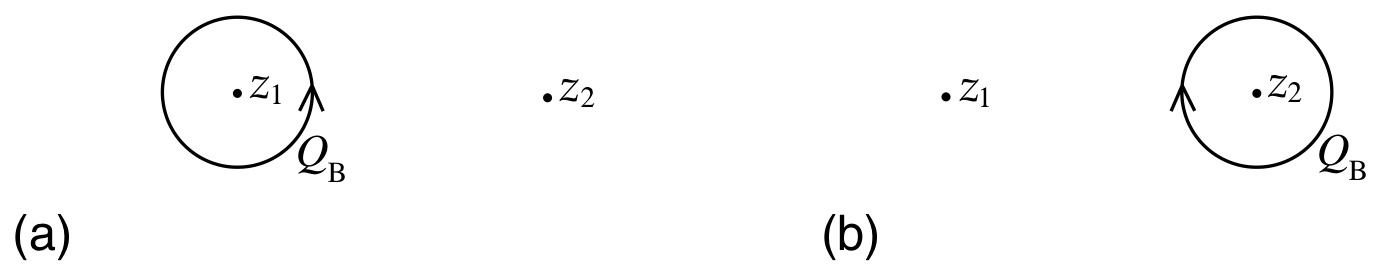
\includegraphics[width=0.8\textwidth]{figure/Fig12.2.jpg}
	\caption{Moving the PCO. The contour around $z_1$ in (a) is pulled around the sphere until it becomes a contour around $z_2$ in (b).}
	\label{fig:12.2}
\end{figure}

Consider now
\begin{equation}
	\lim_{z\to 0}\mathcal{X}(z)\,V_{-1}(0) \:, \label{12.5.11}
\end{equation}
where for convenience we concentrate on the holomorphic side. The $-1$ picture vertex operator is $\me^{-\phi}\mathcal{O}$ with $\mathcal{O}$ a matter superconformal primary. Consider now the term in $\mathcal{X}(z)$ that involves the matter fields,
\begin{equation}
	\me^{\phi}T_{\mathrm{F}}^{\mathrm{m}}(z)\,\me^{-\phi}\mathcal{O}(0) = z\,T_{\mathrm{F}}^{\mathrm{m}}(z)\,\mathcal{O}(0) + \mathcal{O}(z^2) \:. \label{12.5.12}
\end{equation}
The $z \to 0$ limit picks out the coefficient of the $z^{-1}$ in the matter OPE, which is precisely $G_{-1/2}\cdot \mathcal{O} = V_0$, the $0$ picture vertex operator. The purely ghost terms in $\mathcal{X}$ vanish as $z \to 0$, so that
\begin{equation}
	\lim_{z\to 0}\mathcal{X}(z)\,V_{-1}(0) = V_0(0) \:. \label{12.5.13}
\end{equation}

\begin{tcolorbox}[breakable]
	\begin{remark}
		\textbf{Derivation of \eqref{12.5.12} and \eqref{12.5.13}.} \textbf{Conventions.} In bosonized form the PCO is $\mathcal X=\me^{\phi}T_{F}^{\mathrm m}+c\,\partial\xi+\frac14\partial\eta\,\me^{2\phi}b+\frac14\partial(\eta\me^{2\phi}b)$. This is Polchinski's form, the translation of \eqref{12.5.4} through \eqref{12.5.5} and \eqref{12.5.7}. The fixed $-1$ picture vertex operator is $c\,\me^{-\phi}\mathcal O$, where $\mathcal O$ is a weight-$\frac12$ superconformal primary. Then
		\begin{align*}
			\me^{\phi}T_{F}^{\mathrm m}(z)\;c\,\me^{-\phi}\mathcal O(0)
			&\eqs{1} z\,c(0)\,T_{F}^{\mathrm m}(z)\mathcal O(0)\bigl(1+\dots\bigr)\\
			&\eqs{2} z\,c\Bigl[\frac{(G_{1/2}\cdot\mathcal O)}{z^{2}}+\frac{(G_{-1/2}\cdot\mathcal O)}{z}+\text{regular}\Bigr]
			\eqs{3} c\,V_{0}(0)+\dots ,\\
			c\,\partial\xi(z)\;c\,\me^{-\phi}\mathcal O(0)&\eqs{4} \text{vanishes as } z\to0 ,\\
			\bigl(\eta\,\me^{2\phi}b\bigr)(z)\;c\,\me^{-\phi}\mathcal O(0)&\eqs{5} \pm z\,\gamma\mathcal O(0)+\dots .
		\end{align*}
		At (1), $\me^{\phi}(z)\me^{-\phi}(0)\sim z^{-(1)(-1)}=z$. At (2), the OPE of $T_{F}^{\mathrm m}$ with the weight-$\frac12$ operator $\mathcal O$ has poles of order at most $2$, with coefficients $G_{r}\cdot\mathcal O$. At (3), $G_{1/2}\cdot\mathcal O=0$ for a primary, which leaves $G_{-1/2}\cdot\mathcal O=V_{0}$. At (4), $c(z)c(0)\sim z\,c\partial c(0)$ vanishes linearly, and $\partial\xi\,\me^{-\phi}$ is nonsingular. At (5), $\me^{2\phi}(z)\me^{-\phi}(0)\sim z^{2}\me^{\phi}(0)$ and $b(z)c(0)\sim1/z$, and $\eta\,\me^{\phi}=\gamma$. The term $\frac14\partial\eta\,\me^{2\phi}b$ therefore vanishes as $z\to0$. The total derivative $\frac14\partial(\eta\me^{2\phi}b)$, however, leaves a finite ghost term proportional to $\gamma\mathcal O$. Thus $\lim_{z\to0}\mathcal X(z)\,c\me^{-\phi}\mathcal O(0)=c\,V_{0}(0)+(\text{const})\,\gamma\mathcal O(0)$. The matter content is $V_{0}$, which is \eqref{12.5.13} in the old covariant form used in the text, where only the matter part is kept. The extra $\gamma\mathcal O$ term is the ghost completion that makes the $0$ picture fixed vertex operator BRST invariant. Its sign and normalization depend on the cocycle conventions and are not fixed here. So the statement in the text that the purely ghost terms vanish is true for the matter factor, not for the full BRST vertex operator.
	\end{remark}
\end{tcolorbox}

In the bosonic $n$-point amplitude with two $-1$ picture operators and $(n-2)$ $0$ picture operators, we can pull a PCO out of each of the latter to be left with $(n-2)$ PCOs and $n$ vertex operators, all of which are in the $-1$ picture. This is the `natural' picture, the one given by the state--operator mapping. This also shows how to define a general tree-level amplitude, with $n_{\mathrm{B}}$ bosons and $n_{\mathrm{F}}$ (which must be even) fermions. Put all the bosons in the natural $-1$ picture, all the fermions in the natural $-1/2$ picture, and include $(n_{\mathrm{B}} + \frac{1}{2}n_{\mathrm{F}} - 2)$ PCOs. By taking some of the PCOs coincident with vertex operators, possibly more than one PCO at the same vertex operator, one obtains a representation with the vertex operators in higher pictures.

Finally, let us tie up a loose end. The operator product \eqref{12.4.18} is just the product of two spacetime supersymmetry currents, $V_{\alpha} \equiv j_{\alpha}$. By the Ward identity and the supersymmetry algebra, we would expect the $z^{-1}$ term to be the translation current. Instead it is $\me^{-\phi}\psi^{\mu}$. However, this is the zero-momentum vector vertex operator in the $-1$ picture; if we move a PCO to the operator we get the $0$ picture $\del X^{\mu}$ which is indeed the translation current. So the algebra is correct. The $(1,0)$ operator $\me^{-\phi}\psi^{\mu}$ is the translation current; which picture it appears in has no effect on the physics.

\subsection*{Super-Riemann Surfaces}

The preceding discussion suggests a natural generalization to all orders of perturbation theory. That is, string amplitudes are given by an integral over moduli space and the ghost plus matter path integral with the following insertions: the appropriate vertex operator for each incoming or outgoing string in the natural $-1$ or $-1/2$ picture, the $b$-ghosts for the measure on moduli space as in the bosonic string, plus the appropriate number of PCOs to give a sensible path integral. At genus $g$, the Riemann--Roch theorem gives the number of $\beta$ zero modes minus the number of $\gamma$ zero modes as $2g - 2$. Equivalently, the total $\phi$ charge of the insertions must be $2g - 2$. To obtain this, the total number of PCOs must be
\begin{equation}
	n_{\mathcal{X}} = 2g - 2 + n_{\mathrm{B}} + \frac{n_{\mathrm{F}}}{2} \:, \label{12.5.14}
\end{equation}
at arbitrary points; this is for the open string or one side of the closed string. The same formal arguments as in the case of the bosonic string show that this defines a consistent unitary theory. In particular, the PCOs are BRST-invariant and do not affect the decoupling of null states.

\begin{tcolorbox}[breakable]
	\begin{remark}
		\textbf{Derivation of \eqref{12.5.14}.} The Riemann--Roch theorem for holomorphic weight-$\lambda$ fields on a genus-$g$ surface states that the number of zero modes of the weight-$\lambda$ field minus that of its weight-$(1-\lambda)$ partner is $(2\lambda-1)(g-1)$. For $\beta$ ($\lambda=\frac32$) and $\gamma$ ($1-\lambda=-\frac12$) this gives
		\begin{align*}
			n_{\beta}-n_{\gamma}&\eqs{1} (2\cdot\tfrac32-1)(g-1)=2g-2 ,\\
			\sum_{\text{insertions}}q_{\phi}&\eqs{2} 2g-2 ,\qquad\text{i.e.}\qquad n_{\mathcal X}-n_{\mathrm B}-\tfrac12n_{\mathrm F}=2g-2 ,\\
			n_{\mathcal X}&\eqs{3} 2g-2+n_{\mathrm B}+\tfrac12n_{\mathrm F} .
		\end{align*}
		At (1), the Riemann--Roch index was evaluated. At (2), each $\beta$ zero mode needs a $\delta(\beta)\cong\me^{+\phi}$ and each $\gamma$ zero mode a $\delta(\gamma)\cong\me^{-\phi}$ for a nonzero, finite path integral. In bosonized language, the anomaly in the $\phi$ current requires total $\phi$-charge $2g-2$, which is $-2$ on the sphere as used in section~12.4. The PCO carries $+1$ through $\delta(\beta)\cong\me^{\phi}$, a natural NS vertex operator carries $-1$, and a natural R vertex operator carries $-\frac12$. The extra $\xi$ insertion has $\phi$-charge $0$. At (3), the equation was solved for $n_{\mathcal X}$. For $g=0$ and $n_{\mathrm B}=n$ this gives $n-2$ PCOs, as in the tree-level discussion above.
	\end{remark}
\end{tcolorbox}

This prescription is sufficient for all the calculations we will carry out. However, in the remainder of this section we will develop superstring perturbation theory from a more general and geometric point of view. One reason for this is that the picture-changing prescription is rather ad hoc and it would be satisfying to see it derived in some way. Another is that this prescription actually has a subtle ambiguity at higher genus, which is best resolved from the more geometric point of view.

The needed idea is supermoduli space, the space of super-Riemann surfaces (SRSs). These are defined by analogy to Riemann surfaces. Cover the surface with overlapping coordinate patches. The $m$th has coordinates $z_m, \theta_m$. Patches are glued together with superconformal transformations. That is, if patches $m$ and $n$ overlap, identify points such that
\begin{subequations} \label{12.5.15}
	\begin{align}
		z_m &= f_{mn}(z_n) + \theta_n\,g_{mn}(z_n)\,h_{mn}(z_n) \:, \label{12.5.15a} \\
		\theta_m &= g_{mn}(z_n) + \theta_n\,h_{mn}(z_n) \:, \label{12.5.15b} \\
		h_{mn}^2(z_n) &= \del_z f_{mn}(z_n) + g_{mn}(z_n)\,\del_z g_{mn}(z_n) \:. \label{12.5.15c}
	\end{align}
\end{subequations}
\begin{tcolorbox}[breakable]
	\begin{remark}
		\textbf{Derivation of \eqref{12.5.15c}.} A superconformal transition function satisfies \eqref{12.3.6}, $D_{\theta}z_{m}=\theta_{m}D_{\theta}\theta_{m}$, with $D_{\theta}=\partial_{\theta}+\theta\partial_{z}$ acting on the $(z_{n},\theta_{n})$ coordinates, written $(z,\theta)$ here. Suppress the indices $mn$. For $z_{m}=f+\theta gh$ and $\theta_{m}=g+\theta h$,
		\begin{align*}
			D_{\theta}z_{m}&\eqs{1} gh+\theta\,\partial f ,\qquad
			D_{\theta}\theta_{m}\eqs{1} h+\theta\,\partial g ,\\
			\theta_{m}D_{\theta}\theta_{m}&=(g+\theta h)(h+\theta\partial g)
			\eqs{2} gh+\theta\bigl(h^{2}-g\,\partial g\bigr) .
		\end{align*}
		At (1), $\partial_{\theta}(\theta gh)=gh$ and $\theta\partial_{z}(\theta gh)=0$ because $\theta^{2}=0$. At (2), $g\theta\partial g=-\theta g\partial g$, since the odd quantities $g$ and $\theta$ anticommute, and $\theta h\theta\partial g=0$. The $\theta^{0}$ terms agree automatically. Equating the $\theta^{1}$ terms gives $\partial f=h^{2}-g\partial g$, that is
		\[
		\boxed{\;h^{2}=\partial_{z}f+g\,\partial_{z}g\;}
		\]
		which is \eqref{12.5.15c}. This is the patch-to-patch version of \eqref{12.3.9b}. The same computation checks the sphere gluing \eqref{12.5.18}: for $u=1/z$ and $\phi=\mi\theta/z$, $D_{\theta}u=\theta\partial_{z}(1/z)=-\theta/z^{2}$ and $\phi D_{\theta}\phi=(\mi\theta/z)(\mi/z)=-\theta/z^{2}$, so the two agree. It also checks the torus identification \eqref{12.5.21} and the SCKV \eqref{12.5.22}: for $z'=z+\theta\epsilon$ and $\theta'=\theta+\epsilon$, $D_{\theta}z'=\epsilon+\theta$ and $\theta'D_{\theta}\theta'=(\theta+\epsilon)\cdot1$, which are equal. This is the case $f=z$, $g=\epsilon$, $h=1$ of \eqref{12.5.15}.
	\end{remark}
\end{tcolorbox}
\noindent The holomorphic functions $f_{mn}$ and the anticommuting holomorphic functions $g_{mn}$ define the SRS. Two SRSs are equivalent if there is a one-to-one mapping between them such that the respective coordinates are related by a superconformal transformation. Tensor fields are defined by analogy to tensors on an ordinary manifold, as functions in each patch with appropriate transformations between patches. Supermoduli space is the set of equivalence classes of super-Riemann surfaces. The coordinates on supermoduli space are the bosonic (even) moduli $t_j$ and the anticommuting (odd) moduli $\nu_a$. The Riemann--Roch theorem gives the number of odd moduli minus the number of globally defined odd superconformal transformations as $2g - 2$.

Again one can define all of this by Taylor expanding all functions in the anticommuting variables $\theta$ and $\nu_a$. The term in $f_{mn}$ of order $\nu_a^0$ defines an ordinary (not super-) Riemann surface, and everything is expressed in terms of functions on this surface with the component form of the superconformal transformation between patches. Incidentally, $z$ and $\bar{z}$ are no longer formally conjugates of one another on a SRS, particularly in the heterotic string where $\bar{z}$ transforms as the conjugate of equation \eqref{12.5.15} while $z$ transforms as on a `bosonic' Riemann surface. However, if one defines everything by the Taylor expansion then $z$ and $\bar{z}$ are again conjugates on the resulting ordinary Riemann surface.

For any SRS, setting the $\nu_a$ to zero makes the anticommuting $g_{mn}$ vanish and leaves
\begin{subequations} \label{12.5.16}
	\begin{align}
		z_m &= f_{mn}(z_n) \:, \label{12.5.16a} \\
		\theta_m &= \theta_n\,h_{mn}(z_n) \:, \quad h_{mn}^2(z_n) = \del_z f_{mn}(z_n) \:. \label{12.5.16b}
	\end{align}
\end{subequations}
The transformation of $z$ defines a Riemann surface, but that of $\theta$ requires the additional choice of which square root to take in each $h_{mn}$. This choice is known as a spin structure; it is the same data one would need to put a spin-$1/2$ field on the surface. The signs are not all independent. If three patches overlap then the transition functions must satisfy the cocycle condition
\begin{equation}
	h_{mn}\,h_{np}\,h_{pm} = 1 \:. \label{12.5.17}
\end{equation}
Also, a coordinate change $\theta_p \to -\theta_p$ in the patch $p$ changes the signs of all the $h_{pn}$. The net result is that there is one meaningful sign for each nontrivial closed path on the surface, $2g$ for a genus $g$ surface. These define $2^{2g}$ different spin structures, topologically distinct ways to put a spinor field on the surface.

Any sphere is equivalent to the one with two patches $(z,\theta)$, $(u,\phi)$ and transition functions
\begin{equation}
	u = \frac{1}{z} \:, \quad \phi = \frac{\mi\theta}{z} \:. \label{12.5.18}
\end{equation}
Clearly there is just one spin structure. The index theorem implies superconformal Killing transformations. One can look for infinitesimal transformations as in the bosonic case, with the result that $\delta f$ must be at most quadratic in $z$ and $\delta g$ linear in $z$. The general finite transformation is then of the superconformal form with
\begin{equation}
	f(z) = \frac{\alpha z + \beta}{\gamma z + \delta} \:, \quad g(z) = \frac{\epsilon_1 + \epsilon_2 z}{\gamma z + \delta} \:, \label{12.5.19}
\end{equation}
with $\alpha\delta - \beta\gamma = 1$. In particular there are two odd transformations, $\epsilon_1$ and $\epsilon_2$, consistent with the Riemann--Roch theorem. These can be used to fix the odd coordinates of two NS vertex operators to zero.

\begin{tcolorbox}[breakable]
	\begin{remark}
		\textbf{Derivation of the sphere SCKVs \eqref{12.5.19}.} \textbf{Conventions.} An infinitesimal superconformal transformation is generated by an even vector field $v(z)$, a tensor of weight $-1$, and an odd field $\eta(z)$ of weight $-\frac12$, as in \eqref{12.3.10}: $\delta z=\epsilon[v-\mi\theta\eta]$ and $\delta\theta=\epsilon[-\mi\eta+\frac12\theta\partial v]$. Such a transformation is a globally defined SCKV if it is regular in both patches of \eqref{12.5.18}. Transforming to the $(u,\phi)$ patch,
		\begin{align*}
			\delta u&=-\frac{\delta z}{z^{2}}\eqs{1} -\epsilon\,u^{2}\,v(1/u)+\cdots ,\\
			\delta\phi&=\frac{\mi\,\delta\theta}{z}-\frac{\mi\theta\,\delta z}{z^{2}}\eqs{2} \epsilon\,u\,\eta(1/u)+\theta\text{-dependent terms} .
		\end{align*}
		At (1), $u=1/z$. At (2), the odd part of $\delta z$ is proportional to $\theta$, so the second term is regular. Regularity at $u=0$ therefore requires $u^{2}v(1/u)$ and $u\,\eta(1/u)$ to be regular. So $v$ is at most quadratic and $\eta$ at most linear:
		\[
		v=a_{0}+a_{1}z+a_{2}z^{2},\qquad \eta=\epsilon_{1}+\epsilon_{2}z .
		\]
		That is three even and two odd parameters. Exponentiating gives the Möbius $f$ of \eqref{12.5.19} together with $g=(\epsilon_{1}+\epsilon_{2}z)/(\gamma z+\delta)$. The denominator is needed because $g$ has weight $-\frac12$: under the even Möbius part it transforms with $(\partial f)^{1/2}=(\gamma z+\delta)^{-1}$. Riemann--Roch, in the form of the box after \eqref{12.5.14}, predicts $(\#\text{odd moduli})-(\#\text{odd SCKVs})=2g-2=-2$ at $g=0$. There are no odd moduli, so there are $2$ odd SCKVs, in agreement.
	\end{remark}
\end{tcolorbox}

A torus can be described as the $(z,\theta)$ plane modded by a group of rigid superconformal transformations,
\begin{equation}
	(z,\theta) \cong (z + 2\pi, \eta_1\theta) \cong (z + 2\pi\tau, \eta_2\theta) \:. \label{12.5.20}
\end{equation}
The $\eta_1$ and $\eta_2$ are each $\pm 1$, defining the four spin structures. When $\theta$ changes sign around a loop, the bosonic and fermionic components of any superfield will have opposite periodicities, and in particular $T_{\mathrm{F}}$ will be antiperiodic. We thus denote the spin structures $(\mathrm{P},\mathrm{P})$, $(\mathrm{P},\mathrm{A})$, $(\mathrm{A},\mathrm{P})$, and $(\mathrm{A},\mathrm{A})$, giving the $z \to z + 2\pi$ periodicity first. The periodicities on the right-moving side have the same form, with $\bar{\tau}$ the conjugate of $\tau$ but with independent $\tilde{\eta}_1$ and $\tilde{\eta}_2$.

On a torus the only holomorphic functions are the constants, so $\beta$ and $\gamma$ zero modes are possible only in the $(\mathrm{P},\mathrm{P})$ case, in which case there is one of each. There is then an odd supermodulus $\nu$, giving rise to the more general periodicity
\begin{equation}
	(z,\theta) \cong (z + 2\pi, \theta) \cong (z + 2\pi\tau + \theta\nu, \theta + \nu) \:. \label{12.5.21}
\end{equation}
There is also the superconformal Killing vector (SCKV)
\begin{equation}
	(z,\theta) \longrightarrow (z + \theta\epsilon, \theta + \epsilon) \:. \label{12.5.22}
\end{equation}
The number of odd moduli minus the number of SCKVs is zero in all sectors, being $1 - 1$ for the $(\mathrm{P},\mathrm{P})$ spin structure and $0 - 0$ for the others. The modular group and the fundamental region for $\tau$ are the same as in the bosonic string.

Returning to a general SRS, if the positions of $n$ vertex operators are singled out then there is a nontrivial closed curve circling each, less one, giving $2^{2g+n-1}$ spin structures altogether. The additional spin structures come from the choice of R or NS boundary conditions of the external strings. To describe the supermoduli space of SRSs with $n_{\mathrm{B}}$ NS vertex operators and $n_{\mathrm{F}}$ R vertex operators, it is useful to extend the approach used in section 5.4. First in the bosonic case, consider a specific patching together of a Riemann surface, with $n$ marked points. We will define another Riemann surface as equivalent to this one if there is a one-to-one holomorphic mapping between the two which leaves the coordinates of the points invariant. That is, $f(z) - z$ must vanish linearly at the vertex operators. For simplicity we take each operator to be at $z = 0$ in its own tiny patch. Since we are modding by a smaller group, with two real conditions for each vertex operator, we obtain a correspondingly larger coset space, with two additional moduli for each vertex operator. This is similar to the treatment of vertex operator positions in section 5.4, but more abstract. In the superconformal case, we mod out the superconformal transformations for which $f(z) - z$ and $g(z)$ vanish linearly at each NS vertex operator. At each R vertex operator, $g(z)$ has a branch cut, and so it is appropriate to require $f(z) - z$ to vanish linearly in $z$ and $g(z)$ to vanish as $z^{1/2}$. The NS vertex reduces the odd coordinate degrees of freedom by one and so increases the number of inequivalent surfaces: the number of odd moduli increases by one, which we can take to be the $\theta$ coordinate of the operator. The condition for the R vertex operator is essentially half as restrictive, so that there is an additional odd modulus for each pair of R vertex operators. This has no simple interpretation as a vertex operator position; an R vertex operator produces a branch cut in $\theta$, so there can be no well-defined $\theta$ coordinate for the operator. The total number of odd moduli is
\begin{equation}
	n_{\nu} = 2g - 2 + n_{\mathrm{B}} + \frac{n_{\mathrm{F}}}{2} \:. \label{12.5.23}
\end{equation}

\begin{tcolorbox}[breakable]
	\begin{remark}
		\textbf{Derivation of \eqref{12.5.23}.} Odd moduli are odd deformations of the gluing, $\beta$-type zero modes of weight $\frac32$. Odd SCKVs are globally defined $\eta$'s of weight $-\frac12$, $\gamma$-type zero modes. Without punctures, Riemann--Roch, as in the box after \eqref{12.5.14}, gives
		\begin{align*}
			n_{\nu}-n_{\eta}&\eqs{1} 2g-2 ,\\
			n_{\nu}-n_{\eta}&\eqs{2} 2g-2+n_{\mathrm B}\cdot1+n_{\mathrm F}\cdot\tfrac12 ,\\
			n_{\nu}&\eqs{3} 2g-2+n_{\mathrm B}+\tfrac12n_{\mathrm F} .
		\end{align*}
		At (1), Riemann--Roch was applied with $\lambda=\frac32$. At (2), each NS puncture imposes $g(z)=\mathcal O(z)$ on the allowed transformations, one odd condition, so the number of inequivalent odd deformations grows by one. Each R puncture imposes only $g(z)=\mathcal O(z^{1/2})$. Its contribution is half as large, and R punctures come in pairs, since the $\theta$ branch cuts must pair up for the spin structure to be defined. At (3), for amplitudes the punctures remove all odd SCKVs, so $n_{\eta}=0$. For example, the sphere has $n_{\eta}=2$ without punctures, and two NS punctures already fix both. The result \eqref{12.5.23} coincides with the PCO count \eqref{12.5.14}.
	\end{remark}
\end{tcolorbox}

\subsection*{The Measure on Supermoduli Space}

The expression \eqref{5.4.19} for the bosonic string S-matrix now generalizes in a natural way,
\begin{equation}
	\mathcal{S}(1;\dots;n) = \sum_{\chi,\gamma}\me^{-\lambda\chi}\frac{1}{n_{\mathrm{R}}}\int_{\mathfrak{M}_{\chi,\gamma}}\dif^{n_{\mathrm{e}}}t\,\dif^{n_{\mathrm{o}}}\nu\:\biggl\langle \prod_{j=1}^{n_{\mathrm{e}}}B_{j}\prod_{a=1}^{n_{\mathrm{o}}}\delta(B_{a})\prod_{i=1}^{n}\hat{\mathcal{V}}_{i}\biggr\rangle \:. \label{12.5.24}
\end{equation}
The sum is over topologies $\chi$ and spin structures $\gamma$. The integral runs over the corresponding supermoduli space. There are $n_{\mathrm{e}}$ even moduli, $n_{\mathrm{o}}$ odd moduli, and $n$ external strings. The quantity $B_j$ in the ghost insertions is
\begin{equation}
	B_{j} = \sum_{(mn)}\oint_{C_{mn}}\frac{\dif z_m\dif\theta_m}{2\pi\mi}\,B(z_m,\theta_m)\biggl(\frac{\del z_m}{\del t_j} - \frac{\del\theta_m}{\del t_j}\,\theta_m\biggr)_{z_n,\theta_n} \:, \label{12.5.25}
\end{equation}
plus a right-moving piece of the same form; $B_a$ is given by an identical expression with $\nu_a$ replacing $t_j$. The sum again runs over all pairs of overlapping patches $m$ and $n$, clockwise as seen from $m$, with the $z_m$ integration along a contour between the two patches and the $\theta_m$ integral of the usual Berezin form. The $B$ ghost superfield is as in equation \eqref{12.3.25}, $B = \beta + \theta b$.

The logic of this expression is the same as for the earlier bosonic expression. First, the number of commuting and anticommuting ghost insertions is correct for a well-defined path integral. Second, the path integral depends only on the superconformal structure and not on the particular choice of patches and transition functions. In particular it is unchanged if we make a superconformal transformation within a single coordinate patch. The combination $\del z_m + (\del\theta_m)\theta_m$ transforms as a $(-1,0)$ tensor superfield, so the integrand is a $(1/2,0)$ tensor superfield and the integral is invariant. Third, under a change of coordinates in supermoduli space, the product $\prod_{j=1}^{n_{\mathrm{e}}}B_j \prod_{a=1}^{n_{\mathrm{o}}}\delta(B_a)$ transforms as a density, inversely to the measure on supermoduli space. Finally, the commutator of the BRST charge with $B_{j,a}$ is $T_{j,a}$, defined in the same way but with $B$ replaced by
\begin{equation}
	Q_{\mathrm{B}}\cdot B(z) = T(z) = T_{\mathrm{F}}(z) + \theta\,T_{\mathrm{B}}(z) \:. \label{12.5.26}
\end{equation}
The insertion of $T_{j,a}$ generates a relative coordinate transformation of adjacent patches, which is just the derivative with respect to the supermodulus of the worldsheet.

It is interesting to work out the form of the amplitude more explicitly for a special choice of patches and transition functions. Namely, let patch 1 be contained entirely within patch 2, so that the overlap is an annulus. Let the 1-2 transition functions depend only on a single odd modulus $\nu$, as follows:
\begin{equation}
	f_{12}(z_2) = z_2 \:, \quad g_{12}(z_2) = \nu\,\alpha(z_2) \:, \label{12.5.27}
\end{equation}
for some holomorphic function $\alpha(z)$. The ghost factor \eqref{12.5.25} is proportional to
\begin{equation}
	B[\alpha] = \oint \frac{\dif z_1}{2\pi\mi}\,\alpha(z_1)\,\beta(z_1) \:. \label{12.5.28}
\end{equation}
Similarly the path integral depends on $\nu$ only through the insertion
\begin{equation}
	\nu\,T[\alpha] \:, \label{12.5.29}
\end{equation}
where $\beta$ is replaced by $T_{\mathrm{F}}$. We can then perform the integration over $\nu$, so that the net effect of the supermodulus is the insertion in the path integral of
\begin{equation}
	T[\alpha]\,\delta(B[\alpha]) = Q_{\mathrm{B}}\cdot \Theta(B[\alpha]) \:. \label{12.5.30}
\end{equation}
The function $\alpha(z_1)$ is holomorphic in the annular overlap of the patches, but in general cannot be extended holomorphically into the full inner patch $z_1$. If it can, the contour integrals $B[\alpha]$ and $T[\alpha]$ vanish. In this case $\nu$ is not a modulus at all because it can be transformed away. A nontrivial case is
\begin{equation}
	\alpha(z_1) = \frac{1}{z_1 - z_0} \:, \label{12.5.31}
\end{equation}
for which $B[\alpha] = \beta(z_0)$ and the insertion \eqref{12.5.30} just becomes the PCO $\mathcal{X}(z_0)$ (the second term in $\mathcal{X}$ is from normal ordering). Thus, the PCO is the result of integrating out an odd modulus in this special parameterization of the SRSs. Note that the number \eqref{12.5.23} of odd moduli is the same as the number \eqref{12.5.14} of PCOs needed in the ad hoc approach. This provides the desired geometric derivation of the picture-changing prescription.

\begin{tcolorbox}[breakable]
	\begin{remark}
		\textbf{Derivation of \eqref{12.5.30} and of the PCO from \eqref{12.5.31}.} \textbf{Conventions.} $\nu$ is a single odd modulus with Berezin integral $\int\dif\nu\,\nu=1$, and $B[\alpha]$ is Grassmann even, since $\beta$ is commuting. The $\nu$-dependence of the path integral enters only through the insertion $\exp(\nu T[\alpha])=1+\nu T[\alpha]$. Then
		\begin{align*}
			\int\dif\nu\,\bigl(1+\nu T[\alpha]\bigr)\,\delta\bigl(B[\alpha]\bigr)
			&\eqs{1} T[\alpha]\,\delta\bigl(B[\alpha]\bigr)
			\eqs{2} \bigl(Q_{\mathrm B}\cdot B[\alpha]\bigr)\,\Theta'\bigl(B[\alpha]\bigr)\\
			&\eqs{3} Q_{\mathrm B}\cdot\Theta\bigl(B[\alpha]\bigr) ,\\
			B[\alpha]=\oint_{z_{0}}\frac{\dif z_{1}}{2\pi\mi}\,\frac{\beta(z_{1})}{z_{1}-z_{0}}
			&\eqs{4} \beta(z_{0}) ,\qquad T[\alpha]\eqs{4} T_{F}(z_{0}) ,\\
			T[\alpha]\,\delta\bigl(B[\alpha]\bigr)&=T_{F}(z_{0})\,\delta\bigl(\beta(z_{0})\bigr) .
		\end{align*}
		At (1), the Berezin integral picks out the term linear in $\nu$. At (2), \eqref{12.5.26} gives $Q_{\mathrm B}\cdot\beta=T_{F}$, hence $Q_{\mathrm B}\cdot B[\alpha]=T[\alpha]$, and $\delta=\Theta'$. At (3), the chain rule was used: $Q_{\mathrm B}$ acts as a derivation on functions of the commuting operator $B[\alpha]$. At (4), $\alpha=1/(z_{1}-z_{0})$ is holomorphic in the annulus but has a pole at $z_{0}$ inside patch $1$. Shrinking the contour onto $z_{0}$ picks the residue. If instead $\alpha$ extended holomorphically into patch $1$, the integrand would be holomorphic inside and $B[\alpha]=T[\alpha]=0$. The final product $T_{F}\delta(\beta)$ is the first term of $\mathcal X$ in \eqref{12.5.4}. The second term, $-\partial b\,\delta'(\beta)$, is the normal-ordering correction that arises when $T_{F}(z_{0})$ and $\delta(\beta(z_{0}))$ are brought to the same point, as in the box after \eqref{12.5.8}.
	\end{remark}
\end{tcolorbox}

The parameterization \eqref{12.5.27} is always possible locally on supermoduli space. It can also be used globally, with careful treatment of the modular identification and the limits of moduli space. There is a literature on the `ambiguity of superstring perturbation theory,' which arose from parameterizations that did not precisely cover supermoduli space. It appears that superstring perturbation theory to arbitrary order is understood in principle, and certain special amplitudes have been calculated at higher orders of perturbation theory. However, the subject is somewhat unfinished --- a fully explicit proof of the perturbative consistency of the theory seems to be lacking. With the immense progress in nonperturbative string theory, filling this technical gap does not seem to be a key issue.

We derived the bosonic version \eqref{5.4.19} of the measure \eqref{12.5.24} by starting with a path integral over the worldsheet metric, whereas in the present case we have written it down directly. One can partly work backwards to an analogous description as follows. Although $\alpha(z_1)$ cannot be extended holomorphically into patch 1 it can be extended smoothly. It can then be removed by a change of variables in the path integral, but not one that leaves the action invariant. The odd modulus $\nu$ appears in the final action, multiplying $T_{\mathrm{F}}$ and a function that can be regarded as the worldsheet gravitino field. In particular, the PCO can be regarded as coming from a pointlike gravitino, a gauge where the gravitino has delta-function support.

\section{One-Loop Amplitudes}

We will illustrate one-loop superstring calculations with two examples where the low energy limit can be obtained in closed form.

The first is the heterotic string amplitude with four gauge bosons and one antisymmetric tensor. The Green--Schwarz anomaly cancellation requires a one-loop Chern--Simons term
\begin{equation}
	\int B_{\textit{2}}\wedge \operatorname{Tr}_{\mathrm{v}}(F_{\textit{2}}^4) \:. \label{12.6.1}
\end{equation}
We would like to confirm the appearance of this term by an explicit string calculation.

Note first that this can only arise from the $(\mathrm{P},\mathrm{P})$ path integral. This is because it is odd under spacetime parity: written out in components, it involves the ten-dimensional $\epsilon$-tensor. The heterotic string worldsheet action and constraints are invariant under parity. The parity asymmetry of the theory, the fact that the massless fermions are in a $\mathbf{16}$ and not a $\mathbf{16}'$, comes about from the GSO projection in the right-moving R sector, the choice of $\exp(\pi\mi\tilde{F})$ to be $+1$ or $-1$. The $(\mathrm{P},\mathrm{P})$ path integral produces this term in the projection operator. The path integral is then
\begin{align}
	&\quad \Bigl(\frac{2}{\alpha'}\Bigr)^{5/2}g_{\mathrm{c}}^5 \int_{\mathcal{F}}\frac{\dif\tau\dif\bar{\tau}}{8\tau_2}\prod_{i=1}^{5}\int\dif^2 w_i \:\biggl\langle b(0)\tilde{b}(0)\tilde{c}(0)c(0)\,\mathcal{X}(0) \nonumber \\
	&\quad \times \prod_{i=1}^{4}\hat{k}^{-1/2}j^{a_i}\Bigl(\mi e_i\cdot\bar{\del}X + \frac{1}{2}\alpha' k_i\cdot\tilde{\psi}\,e_i\cdot\tilde{\psi}\Bigr)\me^{\mi k_i\cdot X(w_i,\bar{w}_i)} \nonumber \\
	&\quad \times \mi e_{5\mu\nu}\del X^\mu\,\delta(\tilde{\gamma})\,\tilde{\psi}^\nu\,\me^{\mi k_5\cdot X(w_5,\bar{w}_5)}\biggr\rangle_{(\mathrm{P},\mathrm{P})} \:. \label{12.6.2}
\end{align}
The $bc$ ghosts and corresponding measure are the same as in the bosonic string, with an extra $1/2$ from the GSO projection operator. For the $(\mathrm{P},\mathrm{P})$ spin structure there is one PCO and one $-1$ picture vertex operator.

We will consider in order the $\tilde{\psi}^\mu$, $X^\mu$, $bc$, $\beta\gamma$, and $j^a$ path integrals. In the vacuum amplitude the $\tilde{\psi}^\mu$ path integral vanishes in the $(\mathrm{P},\mathrm{P})$ sector. In terms of a trace, this is due to a cancellation between the R sector ground states. In terms of a path integral it is due to the Berezin integration over the zero mode of $\psi^\mu$ (which exists only for this spin structure). In the latter form it is clear that we need at least ten factors of $\tilde{\psi}$ to obtain a nonzero path integral. In fact, the path integral \eqref{12.6.2} has a maximum of ten $\tilde{\psi}$s, including one from the term
\begin{equation}
	\delta(\tilde{\beta})\,\mi\Bigl(\frac{2}{\alpha'}\Bigr)^{1/2}\tilde{\psi}^\rho\bar{\del}X_\rho \label{12.6.3}
\end{equation}
in the PCO. The relevant path integral is easily obtained from a trace, giving
\begin{equation}
	\biggl\langle \prod_{i=1}^{10}\tilde{\psi}^{\mu_i}\biggr\rangle_{\tilde{\psi},(\mathrm{P},\mathrm{P})} = \epsilon^{\mu_1\dots\mu_{10}}\,\bar{q}^{10/24}\prod_{n=1}^{\infty}(1-\bar{q}^n)^{10} = \epsilon^{\mu_1\dots\mu_{10}}\bigl[\eta(\tau)^{10}\bigr]^* \:. \label{12.6.4}
\end{equation}

\begin{tcolorbox}[breakable]
	\begin{remark}
		\textbf{Derivation of \eqref{12.6.4}.} \textbf{Conventions.} The $(\mathrm P,\mathrm P)$ spin structure is the R sector, periodic in $\sigma^{1}$, with $\exp(\pi\mi\tilde F)$ inserted in the trace, periodic in $\sigma^{2}$. The ten zero modes $\tilde\psi_{0}^{\mu}$ satisfy $\{\tilde\psi_{0}^{\mu},\tilde\psi_{0}^{\nu}\}=\eta^{\mu\nu}$, so $\tilde\psi_{0}^{\mu}=\Gamma^{\mu}/\sqrt2$ on the ground states. The overall normalization of the zero-mode trace is fixed so that the coefficient of $\epsilon^{\mu_{1}\dots\mu_{10}}$ is $1$, as in Polchinski. Then
		\begin{align*}
			\Bigl\langle\prod_{i=1}^{10}\tilde\psi^{\mu_{i}}\Bigr\rangle_{(\mathrm P,\mathrm P)}
			&=\operatorname{Tr}_{\mathrm R}\Bigl[\me^{\pi\mi\tilde F}\,\bar q^{\tilde L_{0}-\tilde c/24}\,\tilde\psi_{0}^{\mu_{1}}\cdots\tilde\psi_{0}^{\mu_{10}}\Bigr]\\
			&\eqs{1} \bar q^{10(1/16-1/48)}\prod_{n=1}^{\infty}(1-\bar q^{n})^{10}\times\operatorname{tr}_{32}\bigl[\Gamma\,2^{-5}\Gamma^{\mu_{1}}\cdots\Gamma^{\mu_{10}}\bigr]\\
			&\eqs{2} \bar q^{10/24}\prod_{n=1}^{\infty}(1-\bar q^{n})^{10}\;\epsilon^{\mu_{1}\dots\mu_{10}}\\
			&=\bigl[\eta(\tau)^{10}\bigr]^{*}\epsilon^{\mu_{1}\dots\mu_{10}} .
		\end{align*}
		At (1), the trace factorizes into oscillators and zero modes. Each fermion contributes the R ground-state energy $\frac1{16}$ minus $\frac{c}{24}=\frac1{48}$. Each oscillator $\tilde\psi^{\mu}_{-n}$ contributes $1-\bar q^{n}$, where the minus sign comes from $\exp(\pi\mi\tilde F)$. On the zero modes $\exp(\pi\mi\tilde F)$ acts as the chirality matrix $\Gamma$. At (2), $\frac1{16}-\frac1{48}=\frac1{24}$. In $\operatorname{tr}(\Gamma\Gamma^{\mu_{1}}\cdots\Gamma^{\mu_{k}})$, fewer than ten distinct matrices give a product that is traceless. For $\mu_{i}$ a permutation of $0,\dots,9$, the trace is $\operatorname{sgn}\times\operatorname{tr}(\Gamma^{2})=\pm32$, which gives $\epsilon^{\mu_{1}\dots\mu_{10}}$ with the stated normalization. This is why at least ten $\tilde\psi$ insertions are needed, and why the result is parity odd.
	\end{remark}
\end{tcolorbox}

\noindent The $X^\mu$ path integral is then reduced to
\begin{equation}
	\biggl\langle \del X^\mu(w_5)\,\bar{\del}X^\rho(0)\prod_{i=1}^{5}\me^{\mi k_i\cdot X(w_i,\bar{w}_i)}\biggr\rangle_X \:, \label{12.6.5}
\end{equation}
the gradients coming from the tensor vertex operator and the PCO.

To make things simple we now take the $k_i \to 0$ limit. Contractions between the gradients and exponentials, and among the exponentials, are then suppressed. Only the contraction between the gradients survives, $-\alpha'/8\pi\tau_2$ from the background charge term $\alpha'(\operatorname{Im} w_{ij})^2/4\pi\tau_2$ in the Green's function \eqref{7.2.3}. The leading term in the expectation value \eqref{12.6.5} is then
\begin{align}
	&\quad -\mi(2\pi)^{10}\delta^{10}\Bigl(\sum_{i=1}^{5}k_i\Bigr)\frac{\eta^{\mu\rho}\alpha'}{8\pi\tau_2}(4\pi^2\alpha'\tau_2)^{-5}|\eta(\tau)|^{-20}(4\pi^2\alpha'\tau_2)^{10} \nonumber \\
	&= -\mi(2\pi)^{10}\delta^{10}\Bigl(\sum_{i=1}^{5}k_i\Bigr)\frac{\eta^{\mu\rho}\alpha'}{8\pi\tau_2}(4\pi^2\alpha'\tau_2)^5 |\eta(\tau)|^{20} \:. \label{12.6.6}
\end{align}

\begin{tcolorbox}[breakable]
	\begin{remark}
		\textbf{Derivation of \eqref{12.6.6}.} \textbf{Conventions.} $\langle X^{\mu}(w_{1})X^{\nu}(w_{2})\rangle=\eta^{\mu\nu}G'(w_{1},w_{2})$ with $G'$ the torus Green's function \eqref{7.2.3}. The noncompact $X$ path integral with momentum insertions is $\mi(2\pi)^{10}\delta^{10}(\sum k)\,Z_{X}$, where $Z_{X}=(4\pi^{2}\alpha'\tau_{2})^{-5}|\eta(\tau)|^{-20}$ is the torus partition function of ten bosons from chapter~7. At $k\to0$ only the contraction of the two gradients survives. Writing $w_{12}=w_{1}-w_{2}$,
		\begin{align*}
			\partial_{w_{1}}\partial_{\bar w_{2}}G'
			&\eqs{1} \partial_{w_{1}}\partial_{\bar w_{2}}\Bigl[\alpha'\frac{(\operatorname{Im}w_{12})^{2}}{4\pi\tau_{2}}\Bigr]
			=\frac{\alpha'}{4\pi\tau_{2}}\,\partial_{w_{1}}\partial_{\bar w_{2}}\Bigl[-\frac{(w_{12}-\bar w_{12})^{2}}{4}\Bigr]\\
			&\eqs{2} \frac{\alpha'}{4\pi\tau_{2}}\,\partial_{\bar w_{2}}\Bigl[-\frac{w_{12}-\bar w_{12}}{2}\Bigr]
			\eqs{3} -\frac{\alpha'}{8\pi\tau_{2}} .
		\end{align*}
		At (1), the $\vartheta_{1}$ term is the sum of a holomorphic and an antiholomorphic function of $w_{12}$, so the mixed derivative kills it away from $w_{1}=w_{2}$. At $w_{5}=0$ it leaves a contact term $\propto\delta^{2}(w_{5})$, where the PCO meets the tensor vertex operator. Following Polchinski this term is dropped, which amounts to keeping the PCO away from the vertex operators. The constant $k(\tau,\bar\tau)$ drops out. At (2), $\operatorname{Im}w_{12}=(w_{12}-\bar w_{12})/2\mi$ was used. At (3), $\partial_{\bar w_{2}}\bar w_{12}=-1$. So $\langle\partial X^{\mu}\bar\partial X^{\rho}\rangle=-\eta^{\mu\rho}\alpha'/8\pi\tau_{2}$, and
		\[
		\boxed{\;\langle\cdots\rangle_{X}=-\mi(2\pi)^{10}\delta^{10}\bigl(\textstyle\sum_i k_{i}\bigr)\frac{\eta^{\mu\rho}\alpha'}{8\pi\tau_{2}}\,(4\pi^{2}\alpha'\tau_{2})^{-5}\,|\eta(\tau)|^{-20}\;}
		\]
		This is the first line of \eqref{12.6.6} without the extra factor $(4\pi^{2}\alpha'\tau_{2})^{10}$. That factor, and with it the second line $(4\pi^{2}\alpha'\tau_{2})^{5}|\eta|^{20}$, appear to be misprints. The first line does not even equal the second, because the powers of $|\eta|$ differ. The box after \eqref{12.6.17} shows that only the boxed form gives the measure $\dif^{2}\tau/\tau_{2}^{2}$ and the function $\hat f=\eta^{-8}f$ of \eqref{12.6.16} and \eqref{12.6.17}.
	\end{remark}
\end{tcolorbox}

\noindent The $bc$ path integral is
\begin{equation}
	\langle b(0)\tilde{b}(0)\tilde{c}(0)c(0)\rangle_{bc} = |\eta(\tau)|^4 \:, \label{12.6.7}
\end{equation}
just as in the bosonic string. The $\beta\gamma$ path integral is the reciprocal of the right-moving part of this,
\begin{equation}
	\langle \delta(\tilde{\beta}(0))\delta(\tilde{\gamma}(\bar{w}_5))\rangle_{\beta\gamma} = \bigl[\eta(\tau)^{-2}\bigr]^* \:. \label{12.6.8}
\end{equation}

Finally for the current algebra, we need
\begin{equation}
	\hat{k}^{-2}\langle j^{a_1}(w_1)j^{a_2}(w_2)j^{a_3}(w_3)j^{a_4}(w_4)\rangle_g \:. \label{12.6.9}
\end{equation}
We continue to use the convention $\hat{k} = 1/2$ for the rest of the chapter.

Note first that all other expectation values are independent of $w_i$. The integrations over $w_i$ thus have the effect of averaging over $\operatorname{Re}(w_i)$ and so we can replace each current with the corresponding charge, $\hat{Q}^{a_i}$. We can then evaluate the expectation value as a trace. However, a careful treatment of the $k \to 0$ limit shows that an additional contact term is needed when two vertex operators coincide,
\begin{equation}
	j^a(w)\,j^b(0) \longrightarrow \mathcal{T}\bigl[\hat{Q}^a(w)\hat{Q}^b(0)\bigr] - \pi\delta^2(w,\bar{w})\,\delta^{ab} \:. \label{12.6.10}
\end{equation}
To see this, integrate both sides over the region of worldsheet $-\delta < \sigma_2 < \delta$. On the left we have
\begin{equation}
	\frac{\delta^{ab}}{2}\int_{|\sigma_2|<\delta}\dif^2 w\:\frac{1}{w^2}(w\bar{w})^{k\cdot k'} \:, \label{12.6.11}
\end{equation}
where we have introduced small $k$ and $k'$. The $(w\bar{w})^{k\cdot k'}$ factor from the $X^\mu$ path integral then regulates the integral at the origin. We have kept the leading term in the OPE because this is the only one that contributes at small $\delta$. Writing the integrand as
\begin{equation}
	(-1 + k\cdot k')^{-1}\del_w\bigl(w^{-1+k\cdot k'}\bar{w}^{k\cdot k'}\bigr) \:, \label{12.6.12}
\end{equation}
we can integrate by parts to convert this to a surface integral, which is then easily evaluated at $k,k' \to 0$ to give $-2\pi$. On the right, the first term has no singularity that would allow a nonzero limit as $\delta \to 0$ ($\hat{Q}^a$ is conserved, so it is a constant except for the time ordering), and so the delta function is needed.

\begin{tcolorbox}[breakable]
	\begin{remark}
		\textbf{Derivation of the contact term \eqref{12.6.10}--\eqref{12.6.12}.} \textbf{Conventions.} $w=\sigma^{1}+\mi\sigma^{2}$, $\dif^{2}w=2\dif\sigma^{1}\dif\sigma^{2}$, $\partial_{w}=\frac12(\partial_{1}-\mi\partial_{2})$, $\int\dif^{2}w\,\delta^{2}(w,\bar w)=1$, and $\hat k=\frac12$, so that $j^{a}(w)j^{b}(0)\sim\delta^{ab}/2w^{2}$. Let $\varepsilon=k\cdot k'$ and $v=w^{-1+\varepsilon}\bar w^{\varepsilon}$. For small $\delta$ the strip may be taken infinite in $\sigma^{1}$, since the integrand falls off away from the origin. Then
		\begin{align*}
			\partial_{w}v&\eqs{1} (-1+\varepsilon)\,w^{-2}(w\bar w)^{\varepsilon} ,\\
			\int_{|\sigma^{2}|<\delta}\dif^{2}w\,\partial_{w}v
			&\eqs{2} \int\dif\sigma^{1}\dif\sigma^{2}\,(\partial_{1}-\mi\partial_{2})v
			=-\mi\int\dif\sigma^{1}\Bigl[v\Bigr]_{\sigma^{2}=-\delta}^{\sigma^{2}=+\delta}\\
			&\eqs{3} -\mi\int_{-\infty}^{\infty}\dif\sigma^{1}\Bigl[\frac{1}{\sigma^{1}+\mi\delta}-\frac{1}{\sigma^{1}-\mi\delta}\Bigr]
			=-\mi\int\dif\sigma^{1}\frac{-2\mi\delta}{(\sigma^{1})^{2}+\delta^{2}}=-2\pi ,\\
			\frac{\delta^{ab}}{2}\int_{|\sigma^{2}|<\delta}\dif^{2}w\,\frac{(w\bar w)^{\varepsilon}}{w^{2}}
			&\eqs{4} \frac{\delta^{ab}}{2}\,\frac{-2\pi}{-1+\varepsilon}\;\xrightarrow{\;\varepsilon\to0\;}\;\pi\delta^{ab} .
		\end{align*}
		At (1), the power rule was used; this is \eqref{12.6.12}. At (2), $\dif^{2}w\,\partial_{w}=\dif\sigma^{1}\dif\sigma^{2}(\partial_{1}-\mi\partial_{2})$. The $\partial_{1}$ term integrates to the ends of the strip, where $v\to0$ for $0<\varepsilon<\frac12$. At (3), $\varepsilon\to0$ in the boundary values, which is safe because they are evaluated away from the origin. At (4), (1) was divided by $-1+\varepsilon$. The regulator matters only in this way: it justifies the integration by parts through the singularity. Without it, $\int\dif\sigma^{1}w^{-2}=0$ at every fixed $\sigma^{2}\neq0$ would suggest the answer $0$.

		\emph{Sign.} The left side is $+\pi\delta^{ab}$. On the cylinder the current is $j_{w}=(\partial z/\partial w)j(z)=-\mi z\,j(z)$ with $z=\me^{-\mi w}$, so its average over $\sigma^{1}$ is $-\mi j_{0}$. Take $\hat Q^{a}\equiv j^{a}_{0}$, the Hermitian charge with real eigenvalues, which is what enters the lattice sum \eqref{12.6.15}. Then the averaged currents give $\mathcal T[(-\mi\hat Q)(-\mi\hat Q)]=-\mathcal T[\hat Q\hat Q]$. Matching the strip integrals gives $j^{a}j^{b}\to-\bigl(\mathcal T[\hat Q^{a}\hat Q^{b}]-\pi\delta^{2}(w,\bar w)\delta^{ab}\bigr)$. This is \eqref{12.6.10} up to an overall sign, and the overall sign cancels in the four-current function, because $(-\mi)^{4}=1$. The relative minus sign between the charge term and the contact term, which is all that enters \eqref{12.6.13}--\eqref{12.6.14}, is as printed.
	\end{remark}
\end{tcolorbox}

For the product of two currents we would then have
\begin{align}
	\langle j^{a_1}(w_1)j^{a_2}(w_2)\rangle &\longrightarrow \operatorname{Tr}\Bigl[\me^{2\pi\mi\tau H}\,\mathcal{T}\bigl[\hat{Q}^{a_1}(w_1)\hat{Q}^{a_2}(w_2)\bigr]\Bigr] - \delta^{a_1 a_2}\pi\delta^2(w_{12},\bar{w}_{12}) \nonumber \\
	&\longrightarrow \operatorname{Tr}\Bigl[\me^{2\pi\mi\tau H}\,\hat{Q}^{(a_1}\hat{Q}^{a_2)}\Bigr] - \frac{\delta^{a_1 a_2}}{8\pi\tau_2} \:. \label{12.6.13}
\end{align}
In the second line we have used the fact that all other expectation values are independent of the $w_i$, so that the integrations will have the effect of averaging over $w_i$. In the first term this symmetrizes the operators as indicated; in the second it allows us to replace the delta function with its average over the torus. For four currents the combinatorics are conveniently summarized in terms of the generating function
\begin{equation}
	f(q,z) \equiv \langle \exp(z\cdot \bar{\jmath})\rangle = \exp\Bigl(-\frac{z\cdot z}{16\pi\tau_2}\Bigr)\operatorname{Tr}\Bigl[\me^{2\pi\mi\tau H}\me^{z\cdot \hat{Q}}\Bigr] \:, \label{12.6.14}
\end{equation}
where $\bar{\jmath}^a$ is the average over the torus and the dot denotes a sum on $a$. The needed expectation value is the fourth derivative with respect to $z^a$. The trace is most easily carried out in the bosonic form, where it becomes an oscillator sum plus sum over the $\mathrm{SO}(32)$ or $E_8\times E_8$ lattice:
\begin{equation}
	f(q,z) = \eta(\tau)^{-16}\exp\Bigl(-\frac{z\cdot z}{16\pi\tau_2}\Bigr)\sum_{l\in\Gamma}q^{l^2/2}\me^{2^{-1/2}z\cdot l} \:. \label{12.6.15}
\end{equation}

\begin{tcolorbox}[breakable]
	\begin{remark}
		\textbf{Derivation of \eqref{12.6.13}--\eqref{12.6.15}.} The torus has area $\int\dif^{2}w=2\cdot(2\pi)(2\pi\tau_{2})=8\pi^{2}\tau_{2}$. Averaging the contact term over one position gives
		\begin{align*}
			\frac{1}{8\pi^{2}\tau_{2}}\int\dif^{2}w_{12}\,\pi\delta^{2}(w_{12},\bar w_{12})\,\delta^{a_1a_2}&\eqs{1} \frac{\delta^{a_1a_2}}{8\pi\tau_{2}} ,\\
			\frac{\partial^{2}}{\partial z^{a}\partial z^{b}}\Bigl[\me^{-z\cdot z/16\pi\tau_{2}}\operatorname{Tr}\bigl(\me^{2\pi\mi\tau H}\me^{z\cdot\hat Q}\bigr)\Bigr]_{z=0}
			&\eqs{2} \operatorname{Tr}\bigl(\me^{2\pi\mi\tau H}\hat Q^{(a}\hat Q^{b)}\bigr)-\frac{\delta^{ab}}{8\pi\tau_{2}}\operatorname{Tr}\bigl(\me^{2\pi\mi\tau H}\bigr) .
		\end{align*}
		At (1), $\int\dif^{2}w\,\delta^{2}=1$. At (2), the Gaussian contributes $-2\delta^{ab}/16\pi\tau_{2}$, and the exponential of $z\cdot\hat Q$ expanded to second order is automatically symmetrized. This is the second line of \eqref{12.6.13}, including $\operatorname{Tr}(\me^{2\pi\mi\tau H})$ in the normalization of $\langle1\rangle$. With four derivatives, the Gaussian times the trace produces every way of replacing pairs of currents by the contact term $-\delta/8\pi\tau_{2}$. The terms are: no contact, one contact on any of the $6$ pairs, or two contacts in any of the $3$ complete pairings. This is exactly the combinatorics of pairwise contact terms. This is \eqref{12.6.14}.

		For \eqref{12.6.15}, the $\hat k=\frac12$ level-one algebra is realized by sixteen chiral bosons $H^{I}$ with $H^{I}(z)H^{J}(0)\sim-\delta^{IJ}\ln z$. The Cartan currents are $j^{I}=\frac{\mi}{\sqrt2}\partial H^{I}$, and they have OPE $\frac12\delta^{IJ}/z^{2}$, as $\hat k=\frac12$ requires. A state of lattice momentum $l\in\Gamma$ has $L_{0}=\frac12l^{2}$ plus oscillators and charge $\hat Q^{I}=l^{I}/\sqrt2$. The generating function depends only on the conjugacy class of $z$, so we take $z$ in the Cartan subalgebra. Then
		\[
		\operatorname{Tr}\bigl(q^{L_{0}-16/24}\me^{z\cdot\hat Q}\bigr)=\underbrace{q^{-16/24}\prod_{n}(1-q^{n})^{-16}}_{\eta(\tau)^{-16}}\;\sum_{l\in\Gamma}q^{l^{2}/2}\me^{2^{-1/2}z\cdot l} ,
		\]
		and multiplying by the Gaussian gives \eqref{12.6.15}.
	\end{remark}
\end{tcolorbox}

\noindent Gathering all factors, including $(8\pi\tau_2)^5$ from integrating over the $w_i$, the amplitude becomes
\begin{equation}
	-\mi\frac{g_{\mathrm{c}}^5}{\pi\alpha'^3}(2\pi)^{10}\delta^{10}\Bigl(\sum_{i=1}^{5}k_i\Bigr)\,\epsilon^{\mu_1\dots\mu_{10}}k_{1\mu_1}e_{1\mu_2}\dots k_{4\mu_7}e_{4\mu_8}e_{5\mu_9\mu_{10}}\int_{\mathcal{F}}\frac{\dif^2\tau}{\tau_2^2}\,\frac{\del^4 \hat{f}(q,z)}{\del z^{a_1}\dots\del z^{a_4}}\bigg|_{z=0} \:, \label{12.6.16}
\end{equation}
where
\begin{equation}
	\hat{f}(q,z) = \eta(\tau)^{-8}f(q,z) \:. \label{12.6.17}
\end{equation}
\begin{tcolorbox}[breakable]
	\begin{remark}
		\textbf{Assembling \eqref{12.6.16}, and the modular invariance of \eqref{12.6.17}.} \textbf{Conventions.} $\dif\tau\dif\bar\tau=\dif^{2}\tau=2\dif\tau_{1}\dif\tau_{2}$. Each $\int\dif^{2}w_{i}$ over the torus gives the area $8\pi^{2}\tau_{2}$, because the integrand is independent of the $w_{i}$ at $k\to0$. The overall phase, which depends on the ordering of the ten $\tilde\psi$ inside $\epsilon$, is not tracked.

		\emph{Powers of $\eta$.} Collecting \eqref{12.6.4}, the boxed form of \eqref{12.6.6}, \eqref{12.6.7}, \eqref{12.6.8} and \eqref{12.6.15},
		\begin{align*}
			\underbrace{[\eta^{10}]^{*}}_{\tilde\psi}\;\underbrace{|\eta|^{-20}}_{X}\;\underbrace{|\eta|^{4}}_{bc}\;\underbrace{[\eta^{-2}]^{*}}_{\beta\gamma}\;\underbrace{\eta^{-16}}_{f}
			&\eqs{1} \eta^{-10+2-16}\,\bar\eta^{\,10-10+2-2}=\eta^{-8}\cdot\eta^{-16} .
		\end{align*}
		At (1), holomorphic and antiholomorphic powers were collected separately. The right-moving side cancels completely, which is the supersymmetric cancellation of the vacuum amplitude, and the left side gives $\hat f=\eta^{-8}f$. With the printed second line of \eqref{12.6.6}, $|\eta|^{+20}$, neither statement would hold.

		\emph{Powers of $\tau_{2}$, $\alpha'$ and the constant.} The factors are $(2/\alpha')^{5/2}g_{\mathrm c}^{5}$ from \eqref{12.6.2}; $\frac18\tau_{2}^{-1}$ from the measure; $\mi(2/\alpha')^{1/2}$ from the PCO term \eqref{12.6.3}; $-\mi\alpha'/8\pi\tau_{2}$ and $(4\pi^{2}\alpha'\tau_{2})^{-5}$ from $X$; $(8\pi^{2}\tau_{2})^{5}$ from the five integrals; $(\frac12\alpha')^{4}$ from the fermion bilinears; $\mi$ from the tensor vertex operator; and $\hat k^{-2}=4$. Then
		\begin{align*}
			\tau_{2}:&\quad -1-1-5+5=-2 ,\qquad \alpha':\quad -\tfrac52-\tfrac12+1-5+4=-3 ,\\
			\text{number}:&\quad 2^{3}\cdot\frac18\cdot\frac{1}{8\pi}\cdot\Bigl(\frac{8\pi^{2}}{4\pi^{2}}\Bigr)^{5}\cdot\frac1{16}\cdot4\eqs{2} \frac1\pi .
		\end{align*}
		At (2), $2^{5}\cdot4/(8\pi\cdot16)=1/\pi$. This reproduces $\frac{g_{\mathrm c}^{5}}{\pi\alpha'^{3}}\int\dif^{2}\tau/\tau_{2}^{2}$ in \eqref{12.6.16}, up to the phase. The area of each $w$ integral must be $8\pi^{2}\tau_{2}$, as used here. The ``$(8\pi\tau_{2})^{5}$'' in the text has the right power of $\tau_{2}$ but would leave an extra $\pi^{-5}$.

		\emph{Modular invariance.} The measure $\dif^{2}\tau/\tau_{2}^{2}$ is invariant, so we need $D_{4}(\tau)\equiv\partial^{4}_{z}\hat f(q,z)|_{z=0}$ to be invariant. Under $T:\tau\to\tau+1$, $\eta^{-24}$ is invariant, $q^{l^{2}/2}$ is invariant because $\Gamma$ is even, and $\tau_{2}$ is unchanged. For $S$, write $2^{-1/2}z\cdot l=2\pi\mi\,l\cdot y$ with $y=z/(2\sqrt2\pi\mi)$. The theta function of the even self-dual lattice then obeys $\Theta_{\Gamma}(-1/\tau,y/\tau)=\tau^{8}\me^{\mi\pi y^{2}/\tau}\Theta_{\Gamma}(\tau,y)$, by Poisson resummation, with $y^{2}=-z^{2}/8\pi^{2}$. Hence
		\begin{align*}
			\me^{-\frac{(z/\tau)^{2}}{16\pi\operatorname{Im}(-1/\tau)}}\,\Theta_{\Gamma}\Bigl(-\frac1\tau,\frac y\tau\Bigr)
			&\eqs{3} \tau^{8}\exp\Bigl[-\frac{z^{2}\bar\tau}{16\pi\tau\tau_{2}}-\frac{\mi z^{2}}{8\pi\tau}\Bigr]\Theta_{\Gamma}(\tau,y)\\
			&\eqs{4} \tau^{8}\,\me^{-z^{2}/16\pi\tau_{2}}\,\Theta_{\Gamma}(\tau,y) ,\\
			\hat f\Bigl(-\frac1\tau,\frac z\tau\Bigr)&\eqs{5} \tau^{-12}\cdot\tau^{8}\,\hat f(\tau,z)=\tau^{-4}\hat f(\tau,z)\\
			&\quad\Longrightarrow\quad \tau^{-4}D_{4}(-1/\tau)=\tau^{-4}D_{4}(\tau) .
		\end{align*}
		At (3), $\operatorname{Im}(-1/\tau)=\tau_{2}/|\tau|^{2}$. At (4), $-\frac{z^{2}}{16\pi\tau\tau_{2}}\bigl(\bar\tau+2\mi\tau_{2}\bigr)=-\frac{z^{2}}{16\pi\tau\tau_{2}}\,\tau$, since $\bar\tau+2\mi\tau_{2}=\tau$. The non-holomorphic Gaussian is exactly what completes the lattice sum to a covariant object. At (5), $\eta(-1/\tau)^{-24}=\tau^{-12}\eta(\tau)^{-24}$. Then four derivatives with respect to $z$ were taken at $z=0$: the left side gives $\tau^{-4}D_{4}(-1/\tau)$ because its argument is $z/\tau$. So $D_{4}$ is invariant under $S$ and $T$, and the integrand of \eqref{12.6.16} is modular invariant.
	\end{remark}
\end{tcolorbox}
\noindent We leave it as an exercise to show that this is modular-invariant. Substituting $e_{\mu\nu} \to B_{\mu\nu}/2\kappa$ and $k_{[\mu}e_{\nu]} \to -\mi F_{\mu\nu}/2g_{\mathrm{YM}}$ from the normalization of the kinetic terms, including a factor $2^5$ from converting the $\epsilon$-tensor to form notation, and using the relation between the couplings, the amplitude can be concisely summarized by the effective action
\begin{equation}
	-\frac{1}{2^9\pi^6\alpha'}\int B_{\textit{2}}\wedge \int_{\mathcal{F}}\frac{\dif^2\tau}{\tau_2^2}\,\hat{f}(q,F_{\textit{2}}) \:. \label{12.6.18}
\end{equation}
The form integration picks out the term of order $F_{\textit{2}}^4$. The integral can be written as a surface term and given in closed form, using
\begin{equation}
	\frac{\hat{f}(q,F_{\textit{2}})}{\tau_2^2} = -\frac{32\pi\mi}{F_{\textit{2}}\cdot F_{\textit{2}}}\,\frac{\del\hat{f}(q,F_{\textit{2}})}{\del\bar{\tau}} \:. \label{12.6.19}
\end{equation}
Due to modular invariance, only the limit $\tau_2 \to \infty$ contributes. The effective action becomes
\begin{equation}
	-\frac{1}{2^4\pi^5\alpha'}\int B_{\textit{2}}\wedge \frac{1}{F_{\textit{2}}\cdot F_{\textit{2}}}\,\bigl[\hat{f}(q,F_{\textit{2}})\bigr]_{q^0\text{ term}} \:. \label{12.6.20}
\end{equation}
\begin{tcolorbox}[breakable]
	\begin{remark}
		\textbf{Derivation of \eqref{12.6.19} and \eqref{12.6.20}.} In $\hat f(q,F)=\eta^{-24}\me^{-F\cdot F/16\pi\tau_{2}}\sum_{l}q^{l^{2}/2}\me^{2^{-1/2}F\cdot l}$, everything except the Gaussian is holomorphic in $\tau$. With $\tau_{2}=(\tau-\bar\tau)/2\mi$, so that $\partial\tau_{2}/\partial\bar\tau=\mi/2$,
		\begin{align*}
			\frac{\partial\hat f}{\partial\bar\tau}&\eqs{1} \frac{F\cdot F}{16\pi\tau_{2}^{2}}\cdot\frac{\mi}{2}\,\hat f=\frac{\mi F\cdot F}{32\pi\tau_{2}^{2}}\,\hat f
			\quad\Longrightarrow\quad \frac{\hat f}{\tau_{2}^{2}}=-\frac{32\pi\mi}{F\cdot F}\frac{\partial\hat f}{\partial\bar\tau} ,\\
			\int_{\mathcal F}\dif^{2}\tau\,\partial_{\bar\tau}\hat f
			&\eqs{2} \int_{\mathcal F}\dif\tau_{1}\dif\tau_{2}\,(\partial_{1}+\mi\partial_{2})\hat f
			\eqs{3} \mi\int_{-1/2}^{1/2}\dif\tau_{1}\,\hat f(\tau_{1}+\mi L)\Big|_{L\to\infty}
			\eqs{4} \mi\,\bigl[\hat f\bigr]_{q^{0}} ,\\
			-\frac{1}{2^{9}\pi^{6}\alpha'}\int_{\mathcal F}\frac{\dif^{2}\tau}{\tau_{2}^{2}}\hat f
			&\eqs{5} -\frac{1}{2^{9}\pi^{6}\alpha'}\Bigl(-\frac{32\pi\mi}{F\cdot F}\Bigr)\mi\bigl[\hat f\bigr]_{q^{0}}
			=-\frac{1}{2^{4}\pi^{5}\alpha'}\frac{[\hat f]_{q^{0}}}{F\cdot F} .
		\end{align*}
		At (1), the derivative of $-F\cdot F/16\pi\tau_{2}$ is $+F\cdot F/16\pi\tau_{2}^{2}$ times $\partial\tau_{2}/\partial\bar\tau$; this is \eqref{12.6.19}. At (2), $\dif^{2}\tau=2\dif\tau_{1}\dif\tau_{2}$ and $\partial_{\bar\tau}=\frac12(\partial_{1}+\mi\partial_{2})$. At (3), the $\partial_{1}$ term cancels between the edges $\tau_{1}=\pm\frac12$, which are identified by $T$. The two halves of the arc $|\tau|=1$ are mapped into each other by $S$, with opposite orientation. The relevant order of the integrand is modular invariant, as shown in the previous box, so the two halves cancel, and this is the text's ``due to modular invariance''. Only the cutoff edge at $\tau_{2}=L\to\infty$ remains, traversed at the top of $\mathcal F$. At (4), the $\tau_{1}$ integral projects onto the $q^{0}$ term, and there the Gaussian $\to1$. At (5), $(-32\pi\mi)(\mi)=32\pi$ and $32\pi/2^{9}\pi^{6}=1/2^{4}\pi^{5}$. This is the prefactor of \eqref{12.6.20}.
	\end{remark}
\end{tcolorbox}

\noindent Only the lattice momenta with $l^2 = 2$ contribute to the $q^0$ term. These form the adjoint of the gauge group, so the lattice sum reduces to a trace in the adjoint representation and the effective interaction is
\begin{equation}
	-\frac{1}{2^4\pi^5 6!\,\alpha'}\int B_{\textit{2}}\wedge \frac{\operatorname{Tr}_{\mathrm{a}}(F_{\textit{2}}^6)}{F_{\textit{2}}\cdot F_{\textit{2}}} = -\frac{1}{2^4\pi^5 4!\,\alpha'}\int B_{\textit{2}}\wedge \frac{\operatorname{Tr}_{\mathrm{a}}(F_{\textit{2}}^6)}{\operatorname{Tr}_{\mathrm{a}}(F_{\textit{2}}^2)} \:. \label{12.6.21}
\end{equation}
Ordinarily dividing by a form would make no sense, but we know from the discussion of anomalies that $\operatorname{Tr}_{\mathrm{a}}(F_{\textit{2}}^6) \propto F_{\textit{2}}\cdot F_{\textit{2}}\,X_8(F_{\textit{2}})$, so the effective interaction is proportional to $\int B_{\textit{2}}\wedge X_8$ as required by anomaly cancellation (and with the correct coefficient). For $\mathrm{SO}(32)$ the ratio of forms is $\frac{1}{2}\operatorname{Tr}_{\mathrm{v}}(F_{\textit{2}}^4)$; for $E_8\times E_8$ it is
\begin{equation}
	\frac{1}{7200}\Bigl(\bigl[\operatorname{Tr}_{\mathrm{a}_1}(F_{\textit{2}}^2)\bigr]^2 + \bigl[\operatorname{Tr}_{\mathrm{a}_2}(F_{\textit{2}}^2)\bigr]^2 - \operatorname{Tr}_{\mathrm{a}_1}(F_{\textit{2}}^2)\operatorname{Tr}_{\mathrm{a}_2}(F_{\textit{2}}^2)\Bigr) \:. \label{12.6.22}
\end{equation}

\begin{tcolorbox}[breakable]
	\begin{remark}
		\textbf{Derivation of \eqref{12.6.21} and \eqref{12.6.22}.} \textbf{Conventions.} $\operatorname{Tr}_{\mathrm v}(t^{a}t^{b})=\delta^{ab}$, so $F\cdot F=F^{a}F^{a}=\operatorname{Tr}_{\mathrm v}(F^{2})$ for $SO(32)$. Take $F$ in the Cartan subalgebra. With this normalization the adjoint eigenvalues of $F$ are $F\cdot l/\sqrt2$ for the roots $l$, which have $l^{2}=2$; for $SO(32)$ these are $l=\pm e_{i}\pm e_{j}$. The standard trace identities are taken as input: $\operatorname{Tr}_{\mathrm a}F^{6}=15\operatorname{Tr}_{\mathrm v}F^{2}\operatorname{Tr}_{\mathrm v}F^{4}$ for $SO(32)$, and $\operatorname{Tr}F^{6}=\frac{1}{7200}(\operatorname{Tr}F^{2})^{3}$ in the adjoint of $E_{8}$.
		\begin{align*}
			\bigl[\hat f\bigr]_{q^{0}}&\eqs{1} \Bigl[q^{-1}(1+24q+\cdots)\Bigl(1+q\sum_{l^{2}=2}\me^{2^{-1/2}F\cdot l}+\cdots\Bigr)\Bigr]_{q^{0}}
			=24+\sum_{l^{2}=2}\me^{2^{-1/2}F\cdot l}\\
			&\eqs{2} \cdots+\frac{1}{6!}\sum_{l^{2}=2}\Bigl(\frac{F\cdot l}{\sqrt2}\Bigr)^{6}+\cdots=\cdots+\frac{1}{6!}\operatorname{Tr}_{\mathrm a}(F^{6})+\cdots ,\\
			\operatorname{Tr}_{\mathrm a}(F^{2})&\eqs{3} \sum_{l^{2}=2}\frac{(F\cdot l)^{2}}{2}=30\,F\cdot F=\frac{6!}{4!}F\cdot F ,\\
			\frac{\operatorname{Tr}_{\mathrm a}F^{6}}{\operatorname{Tr}_{\mathrm a}F^{2}}&\eqs{4} \frac{15\operatorname{Tr}_{\mathrm v}F^{2}\operatorname{Tr}_{\mathrm v}F^{4}}{30\operatorname{Tr}_{\mathrm v}F^{2}}=\frac12\operatorname{Tr}_{\mathrm v}F^{4}\quad(SO(32)),\\
			\frac{\operatorname{Tr}_{\mathrm a}F^{6}}{\operatorname{Tr}_{\mathrm a}F^{2}}&\eqs{5} \frac{1}{7200}\frac{(\operatorname{Tr}_{\mathrm a_1}F^{2})^{3}+(\operatorname{Tr}_{\mathrm a_2}F^{2})^{3}}{\operatorname{Tr}_{\mathrm a_1}F^{2}+\operatorname{Tr}_{\mathrm a_2}F^{2}}
			=\frac{1}{7200}\bigl(a_{1}^{2}-a_{1}a_{2}+a_{2}^{2}\bigr)\quad(E_{8}\times E_{8}) .
		\end{align*}
		At (1), $\eta^{-24}=q^{-1}(1+24q+\cdots)$, and the lattice sum starts with $1$ from $l=0$ and $q$ from $l^{2}=2$. At (2), only the term of order $F^{6}$ is needed, because $\int B_{\textit 2}\wedge F^{6}/(F\cdot F)$ must be a ten-form. The zero weights of the Cartan directions do not contribute to $\operatorname{Tr}_{\mathrm a}F^{6}$. This is the first form of \eqref{12.6.21}. At (3), for $SO(32)$ the Cartan index runs over $i=1,\dots,16$, and $\sum_{i<j}\sum_{\pm\pm}(\pm F_{i}\pm F_{j})^{2}/2=2\sum_{i<j}(F_{i}^{2}+F_{j}^{2})=2\cdot15\sum_{i}F_{i}^{2}$. This is $30\,F\cdot F$, where $30=n-2$ is the dual Coxeter number, and $6!/4!=30$ gives the second form of \eqref{12.6.21}. The same factor $30=h(E_{8})$ holds for $E_{8}\times E_{8}$. At (4), the $SO(32)$ identity was used. At (5), $F=F_{1}+F_{2}$ splits the adjoint trace into the two factors, with $a_{i}\equiv\operatorname{Tr}_{\mathrm a_i}F^{2}$, and $(a_{1}^{3}+a_{2}^{3})/(a_{1}+a_{2})=a_{1}^{2}-a_{1}a_{2}+a_{2}^{2}$. This is \eqref{12.6.22}. In both cases the division by $\operatorname{Tr}_{\mathrm a}F^{2}$ is exact, which is the factorization $\operatorname{Tr}_{\mathrm a}F^{6}\propto F\cdot F\,X_{8}$ needed for anomaly cancellation.
	\end{remark}
\end{tcolorbox}

\noindent With somewhat more effort one can also find the required curvature terms. That we were able with modest effort to bring this string loop amplitude to a closed form is not too surprising, since this is a very special amplitude whose coefficient is determined by symmetry (anomaly cancellation). However, many of the physically interesting corrections to the low energy effective action can be obtained in a closed form.

Next we consider the heterotic string amplitude with four gauge bosons but without the antisymmetric tensor. In contrast to the previous amplitude, which came only from the $(\mathrm{P},\mathrm{P})$ spin structure, the present one comes only from the other three spin structures: with one fewer vertex operator there are not enough insertions of $\tilde{\psi}$ to saturate the zero modes of the $(\mathrm{P},\mathrm{P})$ path integral. The amplitude is then
\begin{equation}
	\frac{4g_{\mathrm{c}}^4}{\alpha'^2}\int_{\mathcal{F}}\frac{\dif\tau\dif\bar{\tau}}{8\tau_2}\prod_{i=1}^{4}\int\dif^2 w_i \sum_{\gamma\neq(\mathrm{P},\mathrm{P})}\biggl\langle b(0)\tilde{b}(0)\tilde{c}(0)c(0)\prod_{i=1}^{4}\hat{k}^{-1/2}j^{a_i}\Bigl(\mi e_i\cdot\bar{\del}X + \frac{1}{2}\alpha' k_i\cdot\tilde{\psi}\,e_i\cdot\tilde{\psi}\Bigr)\me^{\mi k_i\cdot X(w_i,\bar{w}_i)}\biggr\rangle_{\gamma} \:. \label{12.6.23}
\end{equation}
For these spin structures, all vertex operators are in the $0$ picture and there is no PCO.

We could proceed to calculate in a straightforward way, but the final result simplifies substantially and it would be better to simplify at the start. In fact, this is one amplitude that is much more easily obtained in the light-cone superstring formalism, and so we will effectively convert the calculation to that form.

First, analytically continue the momenta so that $k^0 = k^1 = 0$. To be consistent with the mass-shell condition the momenta must become complex but this will not be a problem. Also, take the polarizations to vanish in the longitudinal directions. The longitudinal degrees of freedom then do not appear in the vertex operators, and so in the $(\mathrm{P},\mathrm{A})$, $(\mathrm{A},\mathrm{P})$, and $(\mathrm{A},\mathrm{A})$ sectors the longitudinal path integrals just give determinants that cancel against the corresponding ghost path integrals. In particular, the combined longitudinal and ghost path integrals for these three sectors are independent of the spin structure, so the net spin structure dependence comes only from the eight transverse $\tilde{\psi}^i$.

Now, we will temporarily change the problem and also add in the $(\mathrm{P},\mathrm{P})$ spin structure for the $\tilde{\psi}^i$, even though in the real amplitude this is multiplied by zero from the $\tilde{\psi}^{0,1}$ zero modes. The sum over four spin structures gives a GSO projection in the transverse $\tilde{\psi}^i$ CFT by itself. Consider the vertex operator $\tilde{\Theta}^\alpha$ for the R ground state, and bosonize:
\begin{equation}
	\tilde{\Theta}^\alpha \longrightarrow \begin{cases}
		\exp\bigl[\frac{1}{2}\mi(\tilde{H}_1 + \tilde{H}_2 + \tilde{H}_3 + \tilde{H}_4)\bigr] = \exp(\mi\tilde{H}'_1) \\
		\exp\bigl[\frac{1}{2}\mi(\tilde{H}_1 + \tilde{H}_2 - \tilde{H}_3 - \tilde{H}_4)\bigr] = \exp(\mi\tilde{H}'_2) \\
		\exp\bigl[\frac{1}{2}\mi(\tilde{H}_1 - \tilde{H}_2 + \tilde{H}_3 - \tilde{H}_4)\bigr] = \exp(\mi\tilde{H}'_3) \\
		\exp\bigl[\frac{1}{2}\mi(\tilde{H}_1 - \tilde{H}_2 - \tilde{H}_3 + \tilde{H}_4)\bigr] = \exp(\mi\tilde{H}'_4)
	\end{cases} \longrightarrow \tilde{\theta}^\alpha \:. \label{12.6.24}
\end{equation}
Precisely for eight $\tilde{\psi}^i$, the linear combinations of scalars appearing in the spin field are themselves scalars of canonical normalization
\begin{equation}
	\tilde{H}'_i(\bar{z})\,\tilde{H}'_j(0) \sim -\delta_{ij}\ln\bar{z} \:. \label{12.6.25}
\end{equation}
\begin{tcolorbox}[breakable]
	\begin{remark}
		\textbf{Derivation of \eqref{12.6.25}.} Write $\tilde H'_{i}=\sum_{a}R_{ia}\tilde H_{a}$ with the rows of $2R$ equal to $(1,1,1,1)$, $(1,1,-1,-1)$, $(1,-1,1,-1)$ and $(1,-1,-1,1)$. Then
		\begin{align*}
			\tilde H'_{i}(\bar z)\tilde H'_{j}(0)&\eqs{1} \sum_{a,b}R_{ia}R_{jb}\bigl(-\delta_{ab}\ln\bar z\bigr)=-(RR^{\mathrm T})_{ij}\ln\bar z
			\eqs{2} -\delta_{ij}\ln\bar z ,\\
			h\bigl(\me^{\mi s\cdot\tilde H}\bigr)&\eqs{3} \frac12 s^{2}=\frac12\cdot4\cdot\Bigl(\frac12\Bigr)^{2}=\frac12 .
		\end{align*}
		At (1), the $\tilde H_{a}$ are orthonormal. At (2), the four sign vectors are mutually orthogonal, since any two differ in exactly two entries, and each has length squared $4$. So $RR^{\mathrm T}=1$ and the $\tilde H'_{i}$ are again canonically normalized. At (3), the spinor weights $s=(\pm\frac12,\pm\frac12,\pm\frac12,\pm\frac12)$ have $s^{2}=1$. For $n$ transverse fermions the spin field has weight $n/16$, which equals $\frac12$, the weight of a free fermion, only for $n=8$. The same rotation relates $(\tilde\psi^{i})$, $(\tilde\Theta^{\alpha})$ and the other chirality. This is $SO(8)$ triality.
	\end{remark}
\end{tcolorbox}
\noindent Thus after bosonizing and going to a new basis for the scalars we can refermionize in terms of free $(0,1/2)$ fields $\tilde{\theta}^\alpha(\bar{z})$. Note that only for eight $\tilde{\psi}^i$ does the spin field have weight $1/2$. Thus we turn the $\tilde{\psi}^i$ path integral into a $\tilde{\theta}^\alpha$ path integral. Moreover, we claim that the spin structures are related as follows:
\begin{equation}
	\frac{1}{2}\sum_{\gamma}\langle\cdots\rangle_{\tilde{\psi},\gamma} = \langle\cdots\rangle_{\tilde{\theta},(\mathrm{P},\mathrm{P})} \:. \label{12.6.26}
\end{equation}
This follows because the spin field $\tilde{\Theta}^\alpha$ survives the GSO projection, implying that it is single-valued on the torus. The periodicity in the time direction implies the insertion of a factor $\exp(\pi\mi\tilde{F}_{\theta})$ in the sum over states, which is appropriate because $\tilde{\theta}^\alpha$ is a spacetime spinor.

Now we come to the payoff: for this spin structure the $\tilde{\theta}^\alpha$ have eight zero modes, and so there must be eight factors of $\tilde{\theta}^\alpha$ to get a nonzero result. We need to refermionize the vertex operators, but this is easy. The spinors appear only in the combination
\begin{equation}
	k_i\,e_j\,\tilde{\psi}^{[i}\tilde{\psi}^{j]} \:, \label{12.6.27}
\end{equation}
where we can antisymmetrize because $e\cdot k = 0$. The product of fermions is just an $\mathrm{SO}(8)$ rotation current, so we can immediately write
\begin{equation}
	\tilde{\psi}^{[i}\tilde{\psi}^{j]} \longrightarrow \frac{1}{4}\tilde{\theta}^{\mathrm{T}}\Gamma^{ij}\tilde{\theta} \:. \label{12.6.28}
\end{equation}
\begin{tcolorbox}[breakable]
	\begin{remark}
		\textbf{Normalization of \eqref{12.6.28}.} \textbf{Conventions.} $\tilde\theta^{\alpha}(\bar z)\tilde\theta^{\beta}(0)\sim\delta^{\alpha\beta}/\bar z$ and $\tilde\psi^{i}(\bar z)\tilde\psi^{j}(0)\sim\delta^{ij}/\bar z$. The $8\times8$ matrices $\Gamma^{ij}=\frac12[\Gamma^{i},\Gamma^{j}]$ on one $SO(8)$ spinor are real and antisymmetric. Both sides of \eqref{12.6.28} must generate the same $SO(8)$ rotation. On a vector,
		\begin{align*}
			\tilde\psi^{i}\tilde\psi^{j}(\bar z)\,\tilde\psi^{k}(0)&\eqs{1} \frac{\delta^{jk}\tilde\psi^{i}-\delta^{ik}\tilde\psi^{j}}{\bar z} ,\\
			\tfrac14\tilde\theta^{\mathrm T}\Gamma^{ij}\tilde\theta(\bar z)\,\tilde\theta^{\gamma}(0)&\eqs{2} \frac{1}{4\bar z}\bigl(\tilde\theta^{\alpha}\Gamma^{ij}_{\alpha\gamma}-\Gamma^{ij}_{\gamma\beta}\tilde\theta^{\beta}\bigr)=-\frac{1}{2\bar z}\bigl(\Gamma^{ij}\tilde\theta\bigr)^{\gamma} ,\\
			\Bigl[\tfrac12\Gamma^{ij},\Gamma^{k}\Bigr]&\eqs{3} \delta^{jk}\Gamma^{i}-\delta^{ik}\Gamma^{j} .
		\end{align*}
		At (1), there are two single contractions, and moving $\tilde\psi^{k}$ past $\tilde\psi^{i}$ costs a sign. At (2), the two contractions of $\tilde\theta^{\gamma}$ with the bilinear were combined using $\Gamma^{ij}_{\gamma\beta}=-\Gamma^{ij}_{\beta\gamma}$. At (3), $\Gamma^{i}\Gamma^{j}\Gamma^{k}-\Gamma^{k}\Gamma^{i}\Gamma^{j}=2\delta^{jk}\Gamma^{i}-2\delta^{ik}\Gamma^{j}$ for $i\neq j$. By (3), $\pm\frac12\Gamma^{ij}$ is the spinor representative of the rotation whose vector representative is (1). The bilinear in (2) acts with exactly this magnitude, which fixes the coefficient $\frac14$. The overall sign is a choice of triality frame.
	\end{remark}
\end{tcolorbox}
\noindent One can check this by taking the OPE of the two sides with $\tilde{\Theta}^\alpha$ and $\tilde{\theta}^\alpha$ respectively. The fermionic terms in the vertex operators then provide precisely the eight $\tilde{\theta}$s needed to saturate the zero modes, with the result
\begin{equation}
	\biggl\langle \prod_{a=1}^{4}\frac{1}{4}\tilde{\theta}^{\mathrm{T}}\Gamma^{i_a j_a}\tilde{\theta}\biggr\rangle_{\tilde{\theta},(\mathrm{P},\mathrm{P})} = \frac{1}{2^8}\epsilon^{\alpha_1\dots\alpha_8}\Gamma^{i_1 j_1}_{\alpha_1\alpha_2}\dots\Gamma^{i_4 j_4}_{\alpha_7\alpha_8} = t^{i_1 j_1\dots i_4 j_4} + \epsilon^{i_1 j_1\dots i_4 j_4} \:. \label{12.6.29}
\end{equation}
Here $t$ is the same tensor \eqref{12.4.25} that appears in the tree-level amplitudes.

\begin{tcolorbox}[breakable]
	\begin{remark}
		\textbf{Checks of \eqref{12.6.29}.} \textbf{Conventions.} The $\tilde\theta$ zero-mode integral is normalized as $\int\dif^{8}\tilde\theta_{0}\,\tilde\theta^{\alpha_{1}}\cdots\tilde\theta^{\alpha_{8}}=\epsilon^{\alpha_{1}\dots\alpha_{8}}$, with oscillator factors cancelling against the other path integrals. The tensor $t$ is normalized by \eqref{12.4.25}, which with $M^{\mu\nu}=k^{\mu}e^{\nu}-e^{\mu}k^{\nu}$ reads $t_{\mu_{1}\nu_{1}\dots}M_{1}^{\mu_{1}\nu_{1}}\cdots M_{4}^{\mu_{4}\nu_{4}}=2\bigl[4\operatorname{tr}(M_{1}M_{2}M_{3}M_{4})-\operatorname{tr}(M_{1}M_{2})\operatorname{tr}(M_{3}M_{4})+2\text{ perms}\bigr]$. For the Pfaffian we use $\operatorname{Pf}(M)=\frac{1}{2^{4}4!}\epsilon^{\alpha_{1}\dots\alpha_{8}}M_{\alpha_{1}\alpha_{2}}\cdots M_{\alpha_{7}\alpha_{8}}$.

		\emph{Prefactor.} Each bilinear carries $\frac14$, and the eight zero modes are saturated only by the product of all four, which gives $(\frac14)^{4}=2^{-8}$. That is the first equality.

		\emph{Evaluating $\epsilon\Gamma\Gamma\Gamma\Gamma$.} The commuting matrices $\Gamma^{12},\Gamma^{34},\Gamma^{56},\Gamma^{78}$ are simultaneously block diagonal on the $\mathbf 8_{s}$. On the block of the weight pair $\pm s$, $\Gamma^{2k-1,2k}=2s_{k}\,J$ with $J=\bigl(\begin{smallmatrix}0&1\\-1&0\end{smallmatrix}\bigr)$. The four pairs have $2s\in\{(1,1,1,1),(1,1,-1,-1),(1,-1,1,-1),(1,-1,-1,1)\}$. Then
		\begin{align*}
			&\operatorname{Pf}\bigl(a\Gamma^{12}+b\Gamma^{34}+c\Gamma^{56}+d\Gamma^{78}\bigr)\\
			&\qquad\eqs{1} (a+b+c+d)(a+b-c-d)(a-b+c-d)(a-b-c+d)\\
			&\qquad\eqs{2} a^{4}+b^{4}+c^{4}+d^{4}-2(a^{2}b^{2}+\cdots)+8abcd ,\\
			&\frac{1}{2^{8}}\epsilon\,\Gamma^{12}\Gamma^{34}\Gamma^{56}\Gamma^{78}\eqs{3} \frac{1}{2^{8}}\cdot16\cdot8=\frac12 ,\\
			&\frac{1}{2^{8}}\epsilon\,\Gamma^{12}\Gamma^{12}\Gamma^{34}\Gamma^{34}\eqs{4} \frac{1}{2^{8}}\cdot64\cdot(-2)=-\frac12 .
		\end{align*}
		At (1), the Pfaffian of a block-diagonal matrix is the product of the blocks' Pfaffians. At (2), the coefficient of $abcd$ is the permanent of the $\pm1$ matrix above, which is $8$. At (3), in $\epsilon MMMM$ the term with one each of $a,b,c,d$ appears $4!$ times, so $\operatorname{Pf}\supset\frac{4!}{2^{4}4!}abcd\,\epsilon\Gamma^{12}\Gamma^{34}\Gamma^{56}\Gamma^{78}$, and the $\epsilon$ contraction is $16\cdot8$. At (4), the coefficient of $a^{2}b^{2}$ in the Pfaffian is $-2$ and appears with multiplicity $\binom42=6$, so the contraction is $-2\cdot2^{4}4!/6=-128$.

		\emph{Comparison with the right side.} For $M_{1}=M_{2}=E^{12}$ and $M_{3}=M_{4}=E^{34}$, where $E^{ij}$ is the unit rotation generator, we have $\operatorname{tr}(E^{12}E^{12})=-2$ and all other traces vanish. So $2^{4}t_{12,12,34,34}=2[-(-2)(-2)]=-8$, giving $t_{12,12,34,34}=-\frac12$. This agrees with (4), and $\epsilon$ vanishes on repeated indices. For four disjoint planes every trace vanishes, so $t_{12,34,56,78}=0$ and the whole of (3) is the $\epsilon$ term. With the normalization of $t$ fixed by \eqref{12.4.25}, the identity therefore reads
		\[
		\boxed{\;\frac{1}{2^{8}}\epsilon^{\alpha_{1}\dots\alpha_{8}}\Gamma^{i_{1}j_{1}}_{\alpha_{1}\alpha_{2}}\cdots\Gamma^{i_{4}j_{4}}_{\alpha_{7}\alpha_{8}}=t^{i_{1}j_{1}\dots i_{4}j_{4}}\pm\frac12\epsilon^{i_{1}j_{1}\dots i_{4}j_{4}}\;}
		\]
		The sign is set by the chirality of $\tilde\theta$. The coefficient of $\epsilon$ in the printed \eqref{12.6.29} should be $\pm\frac12$ rather than $1$. This has no effect on the physics, since the text discards the $\epsilon$ term.
	\end{remark}
\end{tcolorbox}

It remains to separate out the unwanted $(\mathrm{P},\mathrm{P})$ sector of the $\tilde{\psi}$ path integral, but this is easy. It is the only one that is odd under a reflection of one of the transverse directions, so it is responsible for the term $\epsilon^{i_1 j_1\dots i_4 j_4}$. Thus we omit this term, which in any case does not contribute because the momenta with which it contracts are not linearly independent. Further, the tensor $t$ has a unique covariant extension.

The remaining factors are much as in the previous amplitude, leading for $\mathrm{SO}(32)$ to the effective interaction
\begin{equation}
	\frac{1}{2^8\pi^5 4!\,\alpha'}\,t^{\mu\nu\sigma\rho\alpha\beta\gamma\delta}\operatorname{Tr}_{\mathrm{v}}(F_{\mu\nu}F_{\sigma\rho}F_{\alpha\beta}F_{\gamma\delta}) \:. \label{12.6.30}
\end{equation}
For $E_8\times E_8$ one has instead the group theory structure \eqref{12.6.22}. Given the similarity of the $F^4$ amplitude to the $BF^4$ amplitude, the reader may not be surprised that they are in fact related by supersymmetry.

By this same method several other amplitudes can be obtained, including the Type I cylinder with four open string gauge bosons and the Type II torus with four gravitons. In the latter case both the $\psi^i$ and the $\tilde{\psi}^i$ are refermionized, and the tensor structure is the same as for the tree-level amplitude \eqref{12.4.34}, with two $t$ tensors.

The $\tilde{\theta}^\alpha$ are the first free fields carrying a spacetime spinor index that we have encountered. One might have expected these to arise at some earlier stage. In fact the covariant Green--Schwarz superstring theory, with manifest spacetime supersymmetry, has such fields. It is equivalent to the RNS superstring: after putting each theory in the light cone they are related by the refermionization above. However, the constraints and gauge fixing in the Green--Schwarz description are rather more complicated, and so we have chosen not to emphasize this subject.

\subsection*{Nonrenormalization Theorems}

It follows from the preceding calculations that any amplitude with three or fewer massless particles vanishes because there are too few factors of $\theta^\alpha$ to saturate the zero-mode integrations. One consequence is that there is no renormalization of Newton's constant, which can be measured in the three-graviton amplitude.

\begin{tcolorbox}[breakable]
	\begin{remark}
		\textbf{The counting behind the nonrenormalization statements.} After the refermionization \eqref{12.6.28}, each massless vertex operator, on the side where it is refermionized, contains the transverse spinors only through $k_{i}e_{j}\tilde\psi^{[i}\tilde\psi^{j]}\to\frac14k_{i}e_{j}\,\tilde\theta^{\mathrm T}\Gamma^{ij}\tilde\theta$, which is at most two $\tilde\theta$. The $(\mathrm P,\mathrm P)$ path integral of $\tilde\theta$ vanishes unless all eight zero modes are saturated. So:
		\begin{align*}
			8\le\#\tilde\theta\ \text{supplied}\le2n
			\;&\overset{(1)}{\Longrightarrow}\; n\ge4 ,\qquad
			\mathcal A_{n}\propto\prod_{a=1}^{4}\bigl(k_{i_a}e_{j_a}\bigr)\times\cdots
			\eqs{2} \mathcal O(k^{4}) .
		\end{align*}
		At (1), eight zero modes need at least four bilinears, so all one-loop amplitudes with $n\le3$ massless external states vanish. This includes the three-graviton amplitude, whose coefficient defines Newton's constant, and the one- and two-point functions, which would give a potential or a mass. At (2), each bilinear used to saturate a zero mode carries one explicit momentum. The zero modes are constant on the torus, so no compensating $\int\dif^{2}w\,|w|^{-2+k\cdot k'}$ pole arises from them, and the amplitude vanishes at least as $k^{4}$. A potential $\int\dif^{10}x\,(-G)^{1/2}V(\Phi)$ would contribute at $k^{0}$, and so it is not generated.
	\end{remark}
\end{tcolorbox}

It also follows that all amplitudes vanish at least as $k^4$ when $k \to 0$, from the explicit momentum factors in the vertex operators (this kind of argument is subtle because one can obtain offsetting poles from $\int \dif^2 w (w\bar{w})^{-1+k\cdot k'}$, but the necessary singularity in $w$ does not appear here because the zero modes are independent of $\bar{w}$). This has the important physical consequence that the constant background
\begin{equation}
	G_{\mu\nu}(x) = \eta_{\mu\nu} \:, \quad \Phi(x) = \Phi_0 \label{12.6.31}
\end{equation}
around which we are expanding remains a solution of the field equations to one-loop order. No interaction
\begin{equation}
	\int \dif^{10}x\,(-G)^{1/2}\,V(\Phi) \label{12.6.32}
\end{equation}
is generated. Actually we already knew this from the calculation of the one-loop vacuum amplitude in chapter 10, which vanished by cancellation between bosons and fermions. These nonrenormalization theorems have been argued to extend to all orders of string perturbation theory; the details are left to the references.

Nonrenormalization can also be understood from a spacetime point of view. The tree-level action has local supersymmetry. Therefore the loop corrections must respect this symmetry or else the unphysical polarizations of the gravitino will not decouple. However, no interaction of the form \eqref{12.6.32} is allowed by $d=10$, $N=1$ or $N=2$ supersymmetry (the massive IIA supergravity theory \eqref{12.1.24} effectively has such a term after setting the fields $M$ and $F_{\textit{10}}$ to fixed background values, but the dilaton dependence is fixed and corresponds to a tree-level effect). This argument applies to all orders of perturbation theory and in fact it is a nonperturbative (exact) result. The latter fact is very striking, because with the string technology developed so far we have no direct way to understand strings beyond perturbation theory. It should be noted that the leap from `all orders of perturbation theory' to `exact' is quite nontrivial, because in theories with less symmetry there are many examples of corrections that arise only from nonperturbative effects. We will see some of these later.


	\providecommand{\slashed}[1]{\not{#1}}
\chapter{\texorpdfstring{D-Branes}{13 D-Branes}} \label{cha:13}

In chapter 8 we found that a number of new phenomena, unique to string theory, emerged when the theory was toroidally compactified. Most notable were the T-duality of the closed oriented theory and the appearance of D-branes in the $R \to 0$ limit of the open string theory. These subjects become richer still with the introduction of supersymmetry. We will see that the D-branes are BPS states and carry Ramond--Ramond (R--R) charges. We will argue that the Type I, IIA, and IIB string theories are actually different states in a single underlying theory, which also includes states containing general configurations of D-branes. Whereas previously we considered only parallel D-branes all of the same dimension, we now wish to study more general configurations. We will be concerned with the breaking of supersymmetry, the spectrum and effective action of strings stretched between different D-branes, and scattering and bound states of D-branes. In the present chapter we are still in the realm of string perturbation theory, but many of the results will be used in the next chapter to understand the strongly coupled theory.

\section{T-Duality of Type II Strings}

Even in the closed oriented Type II theories, T-duality has an interesting new effect. Compactify a single spatial coordinate $X^9$ in either Type II theory on a circle of radius $R$ and take the $R \to 0$ limit. This is equivalent to the $R \to \infty$ limit in the dual coordinate, whose right-moving part is reflected:
\begin{equation}
	X_{\mathrm{R}}'^9(\bar{z}) = -X_{\mathrm{R}}^9(\bar{z}) \:, \label{13.1.1}
\end{equation}
just as in the bosonic string. By worldsheet superconformal invariance we must also reflect the right-moving worldsheet fermion $\tilde{\psi}^9(\bar{z})$:
\begin{equation}
	\tilde{\psi}'^9(\bar{z}) = -\tilde{\psi}^9(\bar{z}) \:. \label{13.1.2}
\end{equation}
However, this implies that the chirality of the right-moving Ramond sector ground state is reversed: the raising and lowering operators $\tilde{\psi}_0^8 \pm \mi\tilde{\psi}_0^9$ are interchanged. In terms of the standard spinor annihilation and creation operators:
\[
\tilde{d}_{\pm} = \frac{1}{\sqrt{2}}\bigl(\tilde{\psi}_0^8 \pm \mi\tilde{\psi}_0^9\bigr) \:,
\]
the reflection $\tilde{\psi}_0^9 \to -\tilde{\psi}_0^9$ interchanges $\tilde{d}_{+}$ and $\tilde{d}_{-}$. Consequently, the right-moving chirality operator $\bar{\Gamma}_{11}$ flips its overall sign:
\[
\bar{\Gamma}_{11} \longrightarrow -\bar{\Gamma}_{11} \:.
\]
\begin{tcolorbox}[breakable]
	\begin{remark}
		\textbf{Conventions.} As in section 10.2, the right-moving Ramond zero modes obey $\{\tilde\psi^\mu_0,\tilde\psi^\nu_0\}=\eta^{\mu\nu}$, so on the R ground states they act as $\tilde\psi^\mu_0=\Gamma^\mu/\sqrt2$ with $\{\Gamma^\mu,\Gamma^\nu\}=2\eta^{\mu\nu}$, and the chirality is $\bar\Gamma_{11}=\Gamma^0\Gamma^1\cdots\Gamma^9$ built from these zero modes.

		The reflection acts on the operators $\tilde d_\pm$ and on the weight $S_4$ of the $(8,9)$ plane as
		\begin{align*}
			\tilde d_+\tilde d_- &= \tfrac12\bigl(\tilde\psi^8_0+\mi\tilde\psi^9_0\bigr)\bigl(\tilde\psi^8_0-\mi\tilde\psi^9_0\bigr)
			\eqs{1} \tfrac12\Bigl(\tfrac12+\tfrac12-2\mi\,\tilde\psi^8_0\tilde\psi^9_0\Bigr)
			= \tfrac12-\mi\,\tilde\psi^8_0\tilde\psi^9_0 ,\\
			S_4 &\equiv \tilde d_+\tilde d_- -\tfrac12 = -\mi\,\tilde\psi^8_0\tilde\psi^9_0
			\;\xrightarrow{\;\tilde\psi^9_0\to-\tilde\psi^9_0\;}\; +\mi\,\tilde\psi^8_0\tilde\psi^9_0 \eqs{2} \tilde d_-\tilde d_+-\tfrac12 = -S_4 ,\\
			\bar\Gamma_{11} &= 2^5\,\tilde\psi^0_0\tilde\psi^1_0\cdots\tilde\psi^8_0\,\tilde\psi^9_0
			\;\xrightarrow{\;\tilde\psi^9_0\to-\tilde\psi^9_0\;}\; -\bar\Gamma_{11} .
		\end{align*}
		At (1), $(\tilde\psi^8_0)^2=(\tilde\psi^9_0)^2=\tfrac12$ and $\tilde\psi^9_0\tilde\psi^8_0=-\tilde\psi^8_0\tilde\psi^9_0$. At (2), $\{\tilde d_+,\tilde d_-\}=1$ gives $\tilde d_-\tilde d_+ = 1-\tilde d_+\tilde d_-$, so exchanging $\tilde d_+\leftrightarrow\tilde d_-$ is the same as $S_4\to-S_4$. The last line uses $\Gamma^\mu=\sqrt2\,\tilde\psi^\mu_0$ ten times, which gives $2^{10/2}=2^5$, and only the last factor changes sign. Since $\bar\Gamma_{11}=\prod_{a=0}^4(2S_a)$ up to a fixed phase, flipping the one weight $S_4$ flips the chirality: a $\mathbf{16}$ ground state becomes a $\mathbf{16}'$.
	\end{remark}
\end{tcolorbox}
Simply put, T-duality is a spacetime parity operation on just one side (the right-movers) of the worldsheet, and so reverses the relative chiralities of the right- and left-moving Ramond ground states.

If we begin with the Type IIA theory (which has opposite chiralities $\mathbf{16}$ and $\mathbf{16}'$ for the left- and right-moving Ramond sectors) and take the compactification radius to be small, we obtain the Type IIB theory (which has equal chiralities $\mathbf{16}$ and $\mathbf{16}$) at large radius, and vice versa. The same is true if we T-dualize --- that is, carry out the change of variables \eqref{13.1.1} and \eqref{13.1.2} --- on any odd number of dimensions, while T-dualizing on an even number returns one to the Type II theory with which one began. Thus the two Type II theories are related in the same way as the two heterotic theories: in each case the two noncompact theories are different limits of a single space of compactified theories. The Type II relation is even simpler than the heterotic relation, in that one takes the radius to zero without having also to include a Wilson line.

Since the IIA and IIB theories have different R--R fields, T-duality must transform one set into the other. Again focus on T-duality in just the 9-direction. In order to preserve the operator product expansion between $\tilde{\psi}^\mu$ and the spin field, this must act on the left- and right-moving spin fields as:
\begin{equation}
	V_\alpha'(z) = V_\alpha(z) \:, \quad \tilde{V}_\alpha'(\bar{z}) = (\beta_9)_{\alpha\beta}\tilde{V}_\beta(\bar{z}) \:, \label{13.1.3}
\end{equation}
where $\beta_9$ is the parity transformation (9-reflection) on the spinors. It anticommutes with $\Gamma^9$ and commutes with the remaining $\Gamma^\mu$, so $\beta_9 = \Gamma^9\Gamma_{11}$.
\noindent Now consider the effect on the R--R vertex operators:
\begin{equation}
	V\Gamma^{\mu_1\dots\mu_p}\tilde{V} \:. \label{13.1.4}
\end{equation}
The T-duality multiplies the product of $\Gamma$-matrices by $\Gamma^9\Gamma_{11}$ on the right. The $\Gamma_{11}$ just gives $\pm 1$ because the R ground states have definite chirality. The $\Gamma^9$ adds a `9' to the set $\mu_1\dots\mu_p$ if none is present, or removes one if it is present via $(\Gamma^9)^2 = 1$. This is how T-duality acts on the R--R field strengths and potentials, adding or subtracting the index for the dualized dimensions. Thus, if we start from the IIA string we get the IIB R--R fields as follows (up to signs):
\begin{subequations} \label{13.1.5}
	\begin{align}
		C_9 &\longrightarrow C \:, \label{13.1.5a} \\
		C_\mu \:, \; C_{\mu\nu 9} &\longrightarrow C_{\mu 9} \:, \; C_{\mu\nu} \:, \label{13.1.5b} \\
		C_{\mu\nu\lambda} &\longrightarrow C_{\mu\nu\lambda 9} \:, \label{13.1.5c}
	\end{align}
\end{subequations}
where here $\mu$ stands for a nondualized dimension. One could go on, getting $C_{\mu\nu\lambda\omega}$ from $C_{\mu\nu\lambda\omega 9}$ and so on, but these are not independent fields, and give rather the Hodge dual description of the fields listed.
\begin{tcolorbox}[breakable]
	\begin{remark}
		\textbf{Conventions.} The charge-conjugation matrix between $V$ and $\Gamma^{\mu_1\dots\mu_n}$ is suppressed. As in section 12.1, the bispinor component $V\Gamma^{\mu_1\dots\mu_n}\tilde V$ is the vertex operator of the field strength $F_{\mu_1\dots\mu_n}$, and $\Gamma^{\mu_1\dots\mu_n}$ is the antisymmetrized product, equal to $\Gamma^{\mu_1}\cdots\Gamma^{\mu_n}$ for distinct indices. The background is taken independent of $x^9$, as it must be for the T-duality to act simply.

		Writing the old vertex operator in terms of the dual fields,
		\begin{align*}
			V\Gamma^{\mu_1\dots\mu_n}\tilde V
			&\eqs{1} V'\Gamma^{\mu_1\dots\mu_n}\beta_9^{-1}\tilde V'
			\eqs{2} -V'\Gamma^{\mu_1\dots\mu_n}\Gamma^9\Gamma_{11}\tilde V'
			\eqs{3} \mp V'\Gamma^{\mu_1\dots\mu_n}\Gamma^9\tilde V' ,\\
			\Gamma^{\mu_1\dots\mu_n}\Gamma^9 &\eqs{4}
			\begin{cases}
				\Gamma^{\mu_1\dots\mu_n 9} & (9\notin\{\mu_i\}),\\[2pt]
				\Gamma^{\mu_1\dots\mu_{n-1}}(\Gamma^9)^2=\Gamma^{\mu_1\dots\mu_{n-1}} & (\mu_n=9).
			\end{cases}
		\end{align*}
		At (1), \eqref{13.1.3} was inverted. At (2), $\beta_9^{-1}=-\beta_9$ because $\beta_9^2=-1$. At (3), $\Gamma_{11}\tilde V'=\pm\tilde V'$ since the dual R ground state has definite chirality. At (4), for distinct indices the product is already antisymmetric; if a 9 is present it is first moved to the end, at the cost of a sign, and then $(\Gamma^9)^2=\eta^{99}=1$. So a field-strength component with $n$ indices maps to one with $n\pm1$ indices. For $x^9$-independent potentials the map on the potentials follows:
		\begin{align*}
			F_{\mu9}=\partial_\mu C_9 &\;\to\; F_\mu=\partial_\mu C, &
			F_{\mu\nu}=2\partial_{[\mu}C_{\nu]} &\;\to\; F_{\mu\nu9}=2\partial_{[\mu}C_{\nu]9},\\
			F_{\mu\nu\lambda9}=3\partial_{[\mu}C_{\nu\lambda]9} &\;\to\; F_{\mu\nu\lambda}=3\partial_{[\mu}C_{\nu\lambda]}, &
			F_{\mu\nu\lambda\omega}=4\partial_{[\mu}C_{\nu\lambda\omega]} &\;\to\; F_{\mu\nu\lambda\omega9}=4\partial_{[\mu}C_{\nu\lambda\omega]9},
		\end{align*}
		which is \eqref{13.1.5}: $C_9\to C$, $C_\mu\to C_{\mu9}$, $C_{\mu\nu9}\to C_{\mu\nu}$ and $C_{\mu\nu\lambda}\to C_{\mu\nu\lambda9}$. The even-rank IIA field strengths go into the odd-rank IIB ones, and vice versa.
	\end{remark}
\end{tcolorbox}

For T-duality on multiple dimensions replace $\beta_9$ with
\begin{equation}
	\prod_{m}\beta_m \:, \label{13.1.6}
\end{equation}
where $\beta_m = \Gamma_{11}\Gamma^m$ and the product runs over the dualized directions. There are some signs which should be noted but should not distract attention from the main physical point. Since $\beta_m\beta_n = -\beta_n\beta_m$ for $m \neq n$, T-dualities in different directions do not quite commute but differ by a sign in the right-moving R sector:
\begin{equation}
	\beta_m\beta_n = \exp(\pi\mi\tilde{F})\beta_n\beta_m \:, \label{13.1.7}
\end{equation}
where $\tilde{F}$ is the spacetime fermion number of the right-moving state of the string; this is a symmetry that flips the sign of all right-moving R states. Also, we have defined $\beta_m$ so as to preserve the Hermiticity of $\tilde{V}_\alpha$ (that is, it is real in a Majorana basis), but then $\beta_m\beta_m = -1$ and so acting twice with T-duality gives $\exp(\pi\mi\tilde{F})$.
\begin{tcolorbox}[breakable]
	\begin{remark}
		\textbf{Conventions.} The text defines $\beta_9=\Gamma^9\Gamma_{11}$ below \eqref{13.1.3} but $\beta_m=\Gamma_{11}\Gamma^m$ below \eqref{13.1.6}. Since $\Gamma_{11}\Gamma^m=-\Gamma^m\Gamma_{11}$ the two differ by an overall sign. In every box of this chapter we use $\beta_m=\Gamma^m\Gamma_{11}$, matching \eqref{13.1.3}. The relations below are insensitive to the choice, which only changes $\prod_m\beta_m$ by $(-1)^{\#m}$, and this is the brane versus antibrane ambiguity discussed with \eqref{13.2.4}.

		For $m\neq n$,
		\begin{align*}
			\beta_m\beta_n = \Gamma^m\Gamma_{11}\Gamma^n\Gamma_{11} \eqs{1} -\Gamma^m\Gamma^n\Gamma_{11}\Gamma_{11} = -\Gamma^m\Gamma^n \eqs{2} \Gamma^n\Gamma^m = -\beta_n\beta_m ,
		\end{align*}
		where (1) uses $\Gamma_{11}\Gamma^n=-\Gamma^n\Gamma_{11}$ and $\Gamma_{11}^2=1$, and (2) uses $\Gamma^m\Gamma^n=-\Gamma^n\Gamma^m$; the final step reads the first two equalities backwards with $m\leftrightarrow n$. The right-moving spacetime fermion number is $\tilde F=0$ on right-moving NS states and $\tilde F=1$ on right-moving R states, and the $\beta$'s act only on the latter. So on everything they act on, $\exp(\pi\mi\tilde F)=-1$, and
		\begin{equation*}
			\beta_m\beta_n=-\beta_n\beta_m=\exp(\pi\mi\tilde F)\,\beta_n\beta_m ,
		\end{equation*}
		which is \eqref{13.1.7}. Likewise $\beta_m\beta_m=-1=\exp(\pi\mi\tilde F)$ by the second line of the previous box. Each $\beta_m$ is a product of the real matrices $\Gamma^m$ and $\Gamma_{11}$, so it is real, and $\prod_m\beta_m$ is real and orthogonal; this is the Hermiticity statement in the text.
	\end{remark}
\end{tcolorbox}


\section{T-Duality of Type I Strings}

Taking the $R \to 0$ limit of the open and unoriented Type I $\mathrm{SO}(32)$ theory leads to D-branes and orientifold planes by the same arguments as for the bosonic string in chapter 8, which the reader should review. In particular, taking the T-dual on a single dimension leads to a space with 16 D8-branes between two orientifold hyperplanes (O8-planes).

Let us first consider the bulk physics of the T-dual theory, obtained by taking $R \to 0$ and concentrating on a region of the dual spacetime that is far away from the fixed planes and D-branes, as illustrated in Figure~\ref{fig:13.1}. The local physics is that of a closed oriented superstring theory: closed because the open strings live far away on the D-branes; oriented because the orientation projection relates the state of any string to that of its image behind the fixed plane, but does not locally constrain the space of states. Thus the local physics must be that of a Type II theory. In particular there are two gravitinos, and any closed string scattering process will be invariant under the 32 supersymmetries of the Type II theory. Since the Type I theory with which we started has equal left- and right-moving chiralities, taking the T-dual in one dimension makes them opposite: the local physics is the IIA superstring. Taking the T-dual on any odd number of dimensions has the same effect; taking the T-dual on any even number of dimensions gives the IIB theory in the bulk.

\begin{figure}[htbp]
	\centering
	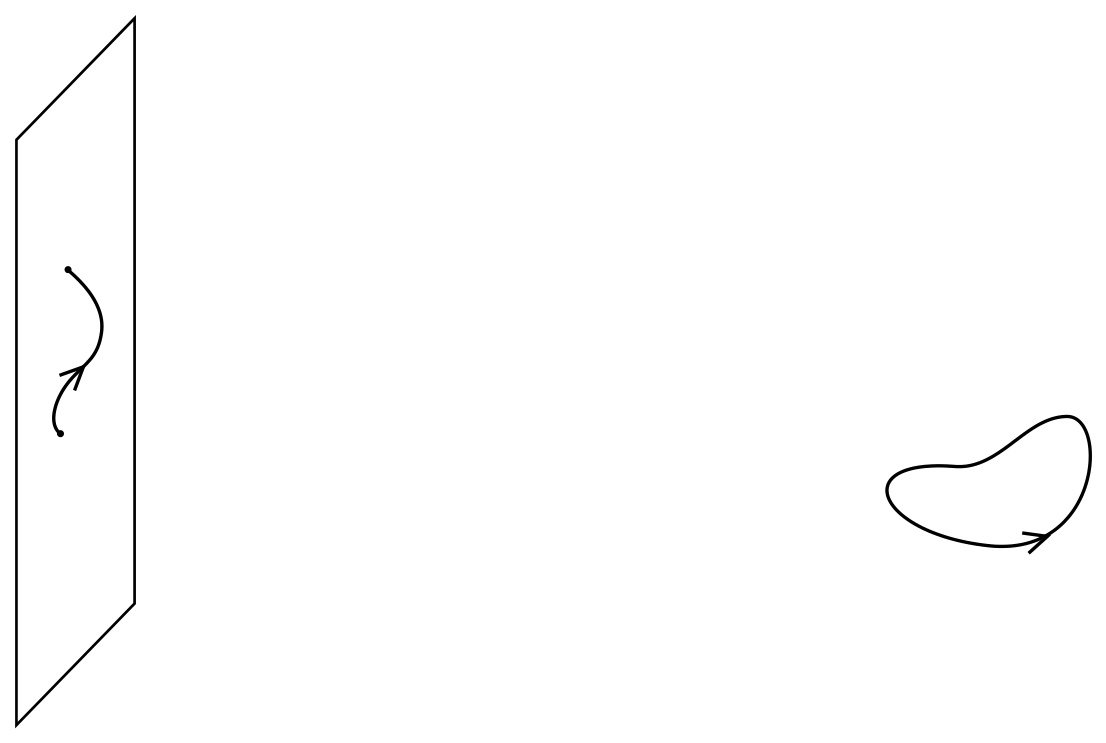
\includegraphics[width=0.65\textwidth]{figure/Fig13.1.jpg}
	\caption{A D-brane, with one attached open string and one closed string moving in the bulk. The physics away from the D-brane is described by a Type II string theory, so the string theory with the D-brane has the physical properties of a state of the Type II theory containing an extended object.}
	\label{fig:13.1}
\end{figure}

Now take the $R \to 0$ limit while concentrating on the neighborhood of one D-brane in the T-dual theory, adjusting the Wilson lines so that again the fixed plane and other D-branes move away in the T-dual spacetime. The low energy degrees of freedom on the D-brane are the massless open string states:
\begin{equation}
	\psi_{-1/2}^\mu\lvert k\rangle_{\mathrm{NS}} \:, \quad \psi_{-1/2}^9\lvert k\rangle_{\mathrm{NS}} \:, \quad \lvert \alpha; k\rangle_{\mathrm{R}} \:. \label{13.2.1}
\end{equation}
As in the bosonic theory, the bosonic states are a gauge field living on the D-brane and the collective coordinates for the D-brane. The fermionic states are the superpartners of these.

Consider now a process where closed strings scatter from the D-brane; this necessarily involves a worldsheet with boundary. Now, the open string boundary conditions are invariant only under $d = 10, N = 1$ supersymmetry. In the original Type I theory, the left-moving worldsheet current for spacetime supersymmetry $V_\alpha(z)$ flows into the boundary and the right-moving current $\tilde{V}_\alpha(\bar{z})$ flows out, so only the total charge $Q_\alpha + \tilde{Q}_\alpha$ of the left- and right-movers is conserved. Under T-duality this becomes:
\begin{equation}
	Q_\alpha' + (\beta_9\tilde{Q}')_\alpha \:. \label{13.2.2}
\end{equation}
The scattering amplitudes of closed strings from the D-brane are invariant only under these 16 supersymmetries.

To see the significance of this, consider first the conservation of momentum. There is a nonzero amplitude for a closed string to reflect backwards from the D-brane, which clearly does not conserve momentum in the direction orthogonal to the D-brane. This occurs because the Dirichlet boundary conditions explicitly break translational invariance. However, from the spacetime point of view the breaking is spontaneous: we are expanding around a D-brane in some definite location, but there are degenerate states with the D-brane translated by any amount (if the D-brane position were a fixed parameter in the Hamiltonian, translation invariance would be explicitly broken, but the D-brane position is a state label and not a parameter). For a spontaneously broken symmetry the consequences are more subtle than for an unbroken symmetry: the apparent violation of the conservation law is related to the amplitude to emit a long-wavelength Goldstone boson. For the D-brane, as for any extended object, the Goldstone bosons are the collective coordinates for its motion. In fact, the nonconservation of momentum is measured by the integral of the corresponding current over the worldsheet boundary:
\begin{equation}
	\frac{1}{2\pi\alpha'}\int_{\del\mathcal{M}}\dif s\:\del_n X'^9 \:, \label{13.2.3}
\end{equation}
which up to normalization is just the ($0$ picture) vertex operator for the collective coordinate, with zero momentum in the Neumann directions.

We conclude by analogy that the D-brane also spontaneously breaks 16 of the 32 spacetime supersymmetries, the ones that are explicitly broken by the open string boundary conditions. The integrals:
\begin{equation}
	\int_{\del\mathcal{M}}\dif s\:V_\alpha' = -\int_{\del\mathcal{M}}\dif s\:(\beta_9\tilde{V}')_\alpha \:, \label{13.2.4}
\end{equation}
which measure the breaking of supersymmetry, are just the vertex operators for the fermionic open string state \eqref{13.2.1}. Thus this state is a goldstino, the Goldstone state associated with spontaneously broken supersymmetry.
\begin{tcolorbox}[breakable]
	\begin{remark}
		\textbf{How a D-brane spontaneously breaks half of the 32 supersymmetries:
		the explicit calculation, from the world-sheet and from supergravity.}
		\medskip

The statement to be derived is that a D$p$-brane of type II string theory, extended along $X^1,\dots,X^p$, is an exact eigenstate of the 16 supercharges
\begin{equation}
Q_\alpha + (\beta^\perp \tilde Q)_\alpha , \qquad \beta^\perp = \beta^{p+1}\beta^{p+2}\cdots\beta^{9},
\tag{D.1}\label{unbroken}
\end{equation}
while the other 16 supercharges are broken spontaneously. Their failure to be conserved in any scattering amplitude equals the amplitude for emitting one extra massless open-string fermion at zero momentum, a goldstino. The derivation proceeds in five steps. A Ward identity on world-sheets with a boundary shows which charges a boundary condition preserves. T-duality turns the type I boundary condition into the D-brane boundary condition and fixes the matrices $\beta^m$. The same Ward identity then identifies the operator that measures the breaking, first for momentum and then for supersymmetry. The spacetime superalgebra shows that exactly 16 supercharges annihilate a brane that saturates the BPS bound. Finally, for the D3-brane, the Killing-spinor equation of type IIB supergravity on the extremal 3-brane solution reproduces the same 16 and the same projection. In every chain of equalities below, a numbered equality sign $\eqs{n}$ is explained in the sentence that follows the chain.

The metric is $\eta_{\mu\nu} = \mathrm{diag}(-1,1,\dots,1)$, the $32\times32$ Dirac matrices satisfy $\{\Gamma^\mu,\Gamma^\nu\} = 2\eta^{\mu\nu}$, and the chirality matrix is $\Gamma = \Gamma^0\Gamma^1\cdots\Gamma^9$. Its square is
\begin{align*}
\Gamma^2 &= (\Gamma^0\cdots\Gamma^9)(\Gamma^0\cdots\Gamma^9)
\eqs{1} (-1)^{45}(\Gamma^0\cdots\Gamma^9)(\Gamma^9\cdots\Gamma^0)\\
&\eqs{2} (-1)^{45}(\Gamma^0)^2(\Gamma^1)^2\cdots(\Gamma^9)^2 = (-1)(-1) = 1 .
\end{align*}
At (1) the second factor was reversed; reversing ten mutually anticommuting matrices takes $10\cdot9/2 = 45$ transpositions. At (2) the adjacent equal pairs were collapsed from the middle outwards. Moving any $\Gamma^\mu$ through $\Gamma$ passes nine anticommuting factors and one commuting factor, so $\Gamma\Gamma^\mu = -\Gamma^\mu\Gamma$. The real Clifford algebra of signature $(9,1)$ is the algebra of real $32\times32$ matrices, so there is a Majorana basis in which every $\Gamma^\mu$ is real. After an orthogonal change of basis, $\Gamma^0$ is antisymmetric and each $\Gamma^i$ is symmetric, and then $\Gamma$ is real and symmetric. The projectors $\frac12(1\pm\Gamma)$ have rank 16 each. The spacetime supersymmetry currents in the $-\frac12$ picture are $\mathcal V_\alpha = e^{-\phi/2}\Theta_\alpha$, holomorphic of weight $(1,0)$ with $\Theta_\alpha$ the spin field, and the antiholomorphic $\tilde{\mathcal V}_\alpha$. They are Hermitian in the Majorana basis and carry 16 real components of definite chirality. The charges
\begin{equation}
Q_\alpha = \frac{1}{2\pi i}\oint dz\,\mathcal V_\alpha , \qquad \tilde Q_\alpha = -\frac{1}{2\pi i}\oint d\bar z\,\tilde{\mathcal V}_\alpha
\tag{D.2}\label{charges}
\end{equation}
are contour independent. The minus sign compensates for $\oint d\bar z/\bar z = -2\pi i$, so that both charges measure a simple pole with the same sign.

Consider now a world-sheet with a boundary. The disk is represented as the upper half plane with its boundary on the real axis. Let $j(z)$ be holomorphic of weight $(1,0)$ and $\tilde j(\bar z)$ antiholomorphic of weight $(0,1)$, and write $\omega = dz\,j - d\bar z\,\tilde j$. The charge $\frac{1}{2\pi i}\oint\omega$ acts on a closed-string vertex operator at an interior point $z_i$ as $\delta V_i = \frac{1}{2\pi i}\oint_{z_i}\omega\,V_i$, the contour being a small counterclockwise circle around $z_i$. Take a disk amplitude with insertions $V_1,\dots,V_n$. Let $D$ be the upper half plane cut off at radius $R$, with small disks around the $z_i$ removed. Since $\omega$ is closed in $D$,
\begin{align*}
0 &= \frac{1}{2\pi i}\oint_{\partial D}\Big\langle \omega\, V_1\cdots V_n\Big\rangle \\
&\eqs{1} \frac{1}{2\pi i}\int_{-R}^{R}dx\,\Big\langle\big[j(x)-\tilde j(x)\big]V_1\cdots V_n\Big\rangle + \frac{1}{2\pi i}\int_{C_R}\Big\langle\omega\,V_1\cdots V_n\Big\rangle \\
&\quad - \sum_i\Big\langle V_1\cdots\delta V_i\cdots V_n\Big\rangle \\
&\eqs{2} \frac{1}{2\pi i}\int_{-\infty}^{\infty}dx\,\Big\langle\big[j(x)-\tilde j(x)\big]V_1\cdots V_n\Big\rangle - \sum_i\Big\langle V_1\cdots\delta V_i\cdots V_n\Big\rangle .
\end{align*}
At (1) the counterclockwise boundary of $D$ was split into three pieces. On the real axis $dz = d\bar z = dx$. The large semicircle $C_R$ remains. The small circles are traversed clockwise, which gives the minus sign. At (2), $R\to\infty$. On the disk the point at infinity is an ordinary boundary point. Under $w = -1/z$ a weight-$(1,0)$ field obeys $j(z) = (dw/dz)\,j(w) = z^{-2}j(w)$ with $j(w)$ regular at $w=0$, so $|\int_{C_R}dz\,j| \le \pi R\cdot R^{-2}\max|j(w)|\to0$, and likewise for $\tilde j$. The result is the Ward identity
\begin{equation}
\sum_{i=1}^n \Big\langle V_1\cdots \delta V_i \cdots V_n\Big\rangle = \frac{1}{2\pi i}\int_{-\infty}^{\infty} dx\,\Big\langle \big[j(x)-\tilde j(x)\big]\, V_1\cdots V_n\Big\rangle .
\tag{D.3}\label{ward}
\end{equation}
The charge is a symmetry of disk amplitudes exactly when $j=\tilde j$ on the boundary. Otherwise the right side is the boundary operator that measures the violation.

Apply this first to the momentum current $j = \frac{i}{\alpha'}\partial X^\mu$, $\tilde j = \frac{i}{\alpha'}\bar\partial X^\mu$, using the bulk propagator $X^\mu(z,\bar z)X^\nu(0)\sim -\frac{\alpha'}{2}\eta^{\mu\nu}\ln|z|^2$. The charge acts on a closed-string tachyon exponential as
\begin{align*}
j(z)\,e^{ik\cdot X}(0) &\eqs{1} \frac{i}{\alpha'}\,\partial_z\Big(-\frac{\alpha'}{2}\ln|z|^2\Big)\,ik^\mu\, e^{ik\cdot X}(0) = \frac{k^\mu}{2z}\,e^{ik\cdot X}(0), \\
\tilde j(\bar z)\,e^{ik\cdot X}(0) &= \frac{k^\mu}{2\bar z}\,e^{ik\cdot X}(0),\\
\delta\, e^{ik\cdot X} &= \frac{1}{2\pi i}\oint dz\,\frac{k^\mu}{2z}\,e^{ik\cdot X} - \frac{1}{2\pi i}\oint d\bar z\,\frac{k^\mu}{2\bar z}\,e^{ik\cdot X} \\
&\eqs{2} \Big(\frac{k^\mu}{2} + \frac{k^\mu}{2}\Big)e^{ik\cdot X} = k^\mu\,e^{ik\cdot X}.
\end{align*}
At (1) the single contraction of $\partial X^\mu$ with the exponential was taken. At (2) the residues $\oint dz/z = 2\pi i$ and $\oint d\bar z/\bar z = -2\pi i$ were used. On the real axis, with $\partial = \frac12(\partial_x - i\partial_y)$ and $\bar\partial = \frac12(\partial_x+i\partial_y)$,
\begin{align*}
j - \tilde j = \frac{i}{\alpha'}(\partial-\bar\partial)X^\mu = \frac{i}{\alpha'}(-i\,\partial_y)X^\mu = \frac{1}{\alpha'}\partial_yX^\mu ,
\end{align*}
so (\ref{ward}) becomes
\begin{equation}
\Big(\sum_i k_i^\mu\Big)\,A = \frac{1}{2\pi i\alpha'}\int dx\,\Big\langle \partial_y X^\mu(x)\,V_1\cdots V_n\Big\rangle ,
\tag{D.4}\label{momward}
\end{equation}
where $A$ is the amplitude. For Neumann conditions $\partial_yX^\mu = 0$ on the boundary, and momentum is conserved. For supersymmetry with a constant spinor $\epsilon^\alpha$, the charges (\ref{charges}) give, for the two combinations,
\begin{align*}
\epsilon\cdot(Q\pm\tilde Q) = \frac{1}{2\pi i}\oint\Big(dz\,\epsilon^\alpha\mathcal V_\alpha \mp d\bar z\,\epsilon^\alpha\tilde{\mathcal V}_\alpha\Big)
\quad\Longrightarrow\quad j - \tilde j\,\Big|_{\rm axis} = \epsilon^\alpha\big(\mathcal V_\alpha \mp \tilde{\mathcal V}_\alpha\big)(x).
\end{align*}
In the type I theory the Neumann conditions $\partial X^\mu = \bar\partial X^\mu$ and $\psi^\mu = \tilde\psi^\mu$ on the real axis make every right-moving field the image of a left-moving one, $\tilde\psi^\mu(\bar z) = \psi^\mu(z^*)$. The same holds for the superconformal ghosts, $\tilde\phi(\bar z) = \phi(z^*)$. After bosonization the spin field is an exponential of the bosons that bosonize pairs of $\psi^\mu$, so it inherits $\tilde\Theta_\alpha(\bar z) = \Theta_\alpha(z^*)$. Hence
\begin{equation}
\mathcal V_\alpha(x) = \tilde{\mathcal V}_\alpha(x)\qquad (x\ \text{real}),
\tag{D.5}\label{typeIbc}
\end{equation}
and both currents carry the same chirality. By (\ref{ward}), $Q+\tilde Q$ is a symmetry of every disk amplitude and $Q-\tilde Q$ is not; these are the 16 supercharges of type I.

T-duality in $X^9$ acts only on right-movers, $\partial X^9 \to \partial X'^9$ and $\bar\partial X^9 \to -\bar\partial X'^9$. On the real axis this gives
\begin{align*}
\partial_xX^9 &= (\partial+\bar\partial)X^9 \;\to\; (\partial-\bar\partial)X'^9 = -i\,\partial_yX'^9, \\
\partial_yX^9 &= i(\partial-\bar\partial)X^9 \;\to\; i(\partial+\bar\partial)X'^9 = i\,\partial_xX'^9 ,
\end{align*}
so the Neumann condition $\partial_yX^9 = 0$ becomes the Dirichlet condition $\partial_xX'^9 = 0$, and $X'^9$ sits at a fixed value $x^9$ on the boundary. The supercurrent $\tilde T_F\propto\tilde\psi_\mu\bar\partial X^\mu$ keeps its form only if $\tilde\psi^9\to-\tilde\psi^9$ as well. In the Ramond sector the zero modes obey $\{\tilde\psi^\mu_0,\tilde\psi^\nu_0\} = \eta^{\mu\nu}$ and act on the ground states $|\alpha\rangle\leftrightarrow\tilde\Theta_\alpha$ as $\Gamma^\mu/\sqrt2$. The reflection is therefore represented on them by a matrix $U$ with $U\Gamma^\mu U^{-1} = \Gamma^\mu$ for $\mu\ne9$ and $U\Gamma^9U^{-1} = -\Gamma^9$. The matrix $\beta^9 = \Gamma^9\Gamma$ satisfies this:
\begin{align*}
\beta^9\Gamma^\mu &= \Gamma^9\Gamma\Gamma^\mu \eqs{1} -\Gamma^9\Gamma^\mu\Gamma \eqs{2} \Gamma^\mu\Gamma^9\Gamma = \Gamma^\mu\beta^9 \qquad(\mu\neq9),\\
\beta^9\Gamma^9 &= \Gamma^9\Gamma\Gamma^9 \eqs{1} -\Gamma^9\Gamma^9\Gamma = -\Gamma^9\beta^9 .
\end{align*}
At (1), $\Gamma$ anticommutes with every $\Gamma^\mu$. At (2), $\Gamma^9$ anticommutes with $\Gamma^\mu$ for $\mu\ne9$. Any other solution $U$ makes $U^{-1}\beta^9$ commute with every $\Gamma^\mu$. The 32-dimensional representation is irreducible, so by Schur's lemma $U^{-1}\beta^9$ is a multiple of the identity and $U = \lambda\beta^9$. Hermiticity of the currents requires $U$ to be real, and preserving the normalization of the ground states requires it to be orthogonal. Both properties hold for $\beta^9$, which fixes $\lambda = \pm1$, and its square follows directly:
\begin{align*}
(\beta^9)^T\beta^9 &= \Gamma^T(\Gamma^9)^T\Gamma^9\Gamma \eqs{1} \Gamma\Gamma^9\Gamma^9\Gamma = 1, \\
\beta^9\beta^9 &= \Gamma^9\Gamma\Gamma^9\Gamma \eqs{2} -\Gamma^9\Gamma^9\Gamma\Gamma = -1, \\
\beta^9\Gamma &= \Gamma^9\Gamma\Gamma = \Gamma^9, \qquad \Gamma\beta^9 = \Gamma\Gamma^9\Gamma \eqs{2} -\Gamma^9 \quad\Longrightarrow\quad \beta^9\Gamma = -\Gamma\beta^9 .
\end{align*}
At (1), $\Gamma$ and $\Gamma^9$ are real and symmetric. At (2), $\Gamma$ anticommutes with $\Gamma^9$. Performing the duality twice therefore gives $-1$ on right-moving spinors, which is $\exp(\pi i\tilde F)$. The alternative $i\beta^9$ squares to $+1$ but is not real. The last line shows that $\beta^9$ flips chirality. The ghost factor $e^{-\tilde\phi/2}$ is unaffected by the duality.

Define the dual currents by $\mathcal V'_\alpha = \mathcal V_\alpha$ and $\tilde{\mathcal V}_\alpha = (\beta^9\tilde{\mathcal V}')_\alpha$, and the dual charges by (\ref{charges}). If $\Gamma\tilde Q = \tilde Q$, then
\begin{align*}
\Gamma\tilde Q' \eqs{1} \Gamma(-\beta^9\tilde Q) \eqs{2} \beta^9\Gamma\tilde Q = \beta^9\tilde Q \eqs{1} -\tilde Q' .
\end{align*}
At (1), $\tilde Q' = (\beta^9)^{-1}\tilde Q = -\beta^9\tilde Q$ because $(\beta^9)^2=-1$. At (2), $\beta^9$ anticommutes with $\Gamma$. The dual charges thus have opposite chirality, so the bulk theory is IIA. The boundary condition (\ref{typeIbc}) becomes
\begin{equation}
\mathcal V'_\alpha(x) = (\beta^9\tilde{\mathcal V}')_\alpha(x) \qquad (x\ \text{real}),
\tag{D.6}\label{dualbc}
\end{equation}
which is consistent because $\beta^9$ maps the chirality of $\tilde{\mathcal V}'$ to that of $\mathcal V'$. The constant matrix $\beta^9$ can be taken inside the contour integrals, so for the two combinations
\begin{align*}
\epsilon\cdot(Q'\pm\beta^9\tilde Q') &= \frac{1}{2\pi i}\oint\Big(dz\,\epsilon^\alpha\mathcal V'_\alpha \mp d\bar z\,\epsilon^\alpha(\beta^9\tilde{\mathcal V}')_\alpha\Big),\\
j-\tilde j\,\Big|_{\rm axis} &= \epsilon^\alpha\big(\mathcal V'_\alpha \mp (\beta^9\tilde{\mathcal V}')_\alpha\big)(x) \eqs{1}
\begin{cases} 0 & (+)\\ 2\epsilon^\alpha\mathcal V'_\alpha(x) & (-)\end{cases}
\end{align*}
where (1) uses (\ref{dualbc}). Inserting this into (\ref{ward}) gives
\begin{align}
\sum_i\Big\langle V_1\cdots\delta_{Q'+\beta^9\tilde Q'}V_i\cdots V_n\Big\rangle &= 0, \tag{D.7}\label{susyward1}\\
\sum_i\Big\langle V_1\cdots\delta_{Q'-\beta^9\tilde Q'}V_i\cdots V_n\Big\rangle &= \frac{1}{\pi i}\int dx\,\Big\langle \epsilon^\alpha\mathcal V'_\alpha(x)\,V_1\cdots V_n\Big\rangle . \tag{D.8}\label{susyward2}
\end{align}
Closed-string scattering off the D8-brane is therefore invariant under $Q'+\beta^9\tilde Q'$ but not under $Q'-\beta^9\tilde Q'$. Defining the dual current instead by $\tilde{\mathcal V}' = \beta^9\tilde{\mathcal V}$ interchanges the two, because $(\beta^9)^{-1} = -\beta^9$. The two choices describe a brane and an antibrane, which carry opposite Ramond--Ramond charge.

Whether the breaking in (\ref{susyward2}) is explicit or spontaneous is settled by first doing the same computation for momentum. In the dual variables the momentum current is $j = \frac{i}{\alpha'}\partial X'^9$, and (\ref{momward}) multiplied by $i$ reads
\begin{equation}
\Big\langle \frac{1}{2\pi\alpha'}\int dx\,\partial_y X'^9(x)\,V_1\cdots V_n\Big\rangle = i\Big(\sum_i k_i^9\Big)A ,
\tag{D.9}\label{dualmom}
\end{equation}
which does not vanish because $\partial_yX'^9\ne0$ on a Dirichlet boundary. Two facts identify the operator on the left. First, it is the T-dual of the zero-momentum vertex operator of the gauge field along 9. The 0-picture gauge-boson vertex operator is proportional to $\int dx\,(i\partial_xX^\mu + 2\alpha'k\cdot\psi\,\psi^\mu)e^{ik\cdot X}$, and
\begin{align*}
\int dx\,\big(i\partial_xX^9 + 2\alpha'k\cdot\psi\,\psi^9\big)e^{ik\cdot X}\Big|_{k=0}
= i\int dx\,\partial_xX^9 \;\to\; i\int dx\,(-i)\partial_yX'^9 = \int dx\,\partial_yX'^9 ,
\end{align*}
using the map of $\partial_xX^9$ derived above. The result is the zero-momentum vertex operator of the massless scalar that describes the transverse position of the brane. Second, it generates translations of the brane. Write $X'^9 = x^9 + Y$ with $Y=0$ on the boundary; then
\begin{align*}
A(x^9) = \int\mathcal DX'\,e^{-S[X']}\prod_i e^{ik_i\cdot X'}
&\eqs{1} \int\mathcal DY\,e^{-S[Y]}\prod_i e^{ik_i^9x^9}e^{ik_i\cdot Y} = e^{ix^9\sum_ik_i^9}A(0), \\
\frac{\partial A}{\partial x^9} &= i\Big(\sum_ik_i^9\Big)A \eqs{2} \Big\langle\frac{1}{2\pi\alpha'}\int dx\,\partial_yX'^9(x)\,V_1\cdots V_n\Big\rangle .
\end{align*}
At (1), the free action depends only on derivatives of $X'$, the measure is shift invariant, and the exponentials factorize. At (2), (\ref{dualmom}) was used. The non-conservation of momentum is thus the amplitude to emit a zero-momentum quantum of the collective coordinate, and inserting that quantum moves the brane infinitesimally. This is the structure of a spontaneously broken symmetry. The ground state, the brane at $x^9$, is not invariant but belongs to a degenerate family of translated ground states. The apparent violation of the conservation law is the emission of the long-wavelength Goldstone mode that moves the system along that family.

Equation (\ref{susyward2}) has the same structure. The massless open-string Ramond state $|\alpha;k\rangle_{\rm R}$ has the $-\frac12$-picture boundary vertex operator $u^\alpha e^{-\phi/2}\Theta_\alpha e^{ik\cdot X}$, subject to $k^2 = 0$ and $k_\mu\Gamma^\mu u = 0$. At $k=0$ both conditions hold trivially, and $\int dx\,\epsilon^\alpha\mathcal V'_\alpha = \int dx\,\epsilon^\alpha e^{-\phi/2}\Theta_\alpha$ is this vertex operator with $u = \epsilon$. The GSO projection keeps $u$ in the chirality of $\mathcal V'$. The variation of any closed-string amplitude under a broken supersymmetry is therefore $1/(\pi i)$ times the amplitude with one extra zero-momentum open-string fermion. That fermion is the goldstino, and the 16 supersymmetries broken explicitly by the world-sheet boundary condition are broken spontaneously in spacetime.

The count of 16 and 16 is exact. The change of basis from $(Q',\tilde Q')$ to $Q'\pm\beta^9\tilde Q'$ is the matrix $\begin{pmatrix}1&\beta^9\\1&-\beta^9\end{pmatrix}$, which is invertible because $\beta^9$ is. The new charges are Hermitian because $\beta^9$ is real, and each set has 16 components in the chiral subspace of $Q'$. For a D$p$-brane, T-dualize $X^{p+1},\dots,X^9$ in turn. Each duality multiplies the right-moving spinor by one more $\beta^m$, the boundary condition becomes $\mathcal V' = \beta^\perp\tilde{\mathcal V}'$, and the argument from (\ref{dualbc}) to (\ref{susyward2}) goes through unchanged with $\beta^\perp$ in place of $\beta^9$. The unbroken charges are then (\ref{unbroken}). The properties of $\beta^\perp$ follow from
\begin{align*}
\beta^m\beta^n = \Gamma^m\Gamma\Gamma^n\Gamma \eqs{1} -\Gamma^m\Gamma^n\Gamma\Gamma = -\Gamma^m\Gamma^n \eqs{2} \Gamma^n\Gamma^m = -\beta^n\beta^m \qquad (m\ne n),
\end{align*}
where (1) uses $\Gamma\Gamma^n = -\Gamma^n\Gamma$ and (2) uses $\Gamma^m\Gamma^n = -\Gamma^n\Gamma^m$; the final step reads the first two equalities backwards with $m\leftrightarrow n$. Thus the order of the dualities changes $\beta^\perp$ only by a sign, which is again the brane versus antibrane choice. With $n = 9-p$ factors,
\begin{align}
(\beta^\perp)^2 = (\beta^{p+1}\cdots\beta^9)(\beta^{p+1}\cdots\beta^9)
&\eqs{1} (-1)^{n(n-1)/2}(\beta^{p+1}\cdots\beta^9)(\beta^9\cdots\beta^{p+1}) \notag\\
&\eqs{2} (-1)^{n(n-1)/2}(-1)^{n} = (-1)^{(9-p)(10-p)/2}. \tag{D.10}\label{bsq}
\end{align}
At (1) the second product was reversed, which takes $n(n-1)/2$ transpositions of anticommuting factors. At (2) the product collapses from the middle using $(\beta^m)^2 = -1$. The matrix $\beta^\perp$ is also real and orthogonal, as a product of real orthogonal matrices, and $\beta^\perp\Gamma = (-1)^{9-p}\Gamma\beta^\perp$ because each factor anticommutes with $\Gamma$. The boundary condition relates currents of opposite chirality in IIA and of the same chirality in IIB. It is therefore consistent for even $p$ in IIA and odd $p$ in IIB.

Next, the superalgebra. Taken as input, with Hermitian charges in the Majorana basis, it reads
\begin{align}
\{Q_\alpha,Q_\beta^\dagger\} &= 2\Big[P_M + \frac{Q^{\rm NS}_M}{2\pi\alpha'}\Big](\Gamma^0\Gamma^M)_{\alpha\beta}, \notag\\
\{\tilde Q_\alpha,\tilde Q_\beta^\dagger\} &= 2\Big[P_M - \frac{Q^{\rm NS}_M}{2\pi\alpha'}\Big](\Gamma^0\Gamma^M)_{\alpha\beta}, \tag{D.11}\label{alg1}\\
\{Q_\alpha,\tilde Q_\beta^\dagger\} &= 2\sum_p\frac{\tau_p}{p!}\,Q^{\rm R}_{M_1\cdots M_p}\,(\beta^{M_1}\cdots\beta^{M_p}\Gamma^0)_{\alpha\beta}. \tag{D.12}\label{alg2}
\end{align}
For a static D$p$-brane along $X^1,\dots,X^p$ in its rest frame, $P_0 = -E$, $P_i = 0$ and $Q^{\rm NS} = 0$. Writing $Z = \tau_pQ^{\rm R}_{1\cdots p}$ and $M = \beta^1\cdots\beta^p\Gamma^0$,
\begin{align*}
\{Q_\alpha,Q_\beta^\dagger\} &= 2P_0(\Gamma^0\Gamma^0)_{\alpha\beta} = 2(-E)(-1)\delta_{\alpha\beta} \\
&= 2E\,\delta_{\alpha\beta} = \{\tilde Q_\alpha,\tilde Q_\beta^\dagger\}, \\
\{Q_\alpha,\tilde Q_\beta^\dagger\} &\eqs{1} \frac{2\tau_p}{p!}\sum_{\sigma\in S_p}Q^{\rm R}_{\sigma(1)\cdots\sigma(p)}\big(\beta^{\sigma(1)}\cdots\beta^{\sigma(p)}\Gamma^0\big)_{\alpha\beta}\\
&\eqs{2} \frac{2\tau_p}{p!}\sum_{\sigma\in S_p}(\mathrm{sgn}\,\sigma)^2\,Q^{\rm R}_{1\cdots p}\,M_{\alpha\beta} = 2Z\,M_{\alpha\beta}, \\
\{\tilde Q_\beta,Q_\alpha^\dagger\} &\eqs{3} \big(\{Q_\alpha,\tilde Q_\beta^\dagger\}\big)^\dagger = 2Z\,M^*_{\alpha\beta} = 2Z\,M_{\alpha\beta} .
\end{align*}
At (1) only permutations of $(1,\dots,p)$ contribute to the index sum. At (2) the charge and the product of anticommuting $\beta$'s each change by $\mathrm{sgn}\,\sigma$ under reordering. At (3), $(AB+BA)^\dagger = B^\dagger A^\dagger + A^\dagger B^\dagger$, and $M$ is real. For $Q_\pm = Q\pm\beta^\perp\tilde Q$, the reality of $\beta^\perp$ gives $(\beta^\perp\tilde Q)^\dagger_\beta = \beta^\perp_{\beta\delta}\tilde Q^\dagger_\delta$, and
\begin{align*}
\{Q_{\pm\alpha},Q_{\pm\beta}^\dagger\}
&= \{Q_\alpha,Q_\beta^\dagger\} + \beta^\perp_{\alpha\gamma}\beta^\perp_{\beta\delta}\{\tilde Q_\gamma,\tilde Q_\delta^\dagger\} \\
&\quad \pm \beta^\perp_{\beta\delta}\{Q_\alpha,\tilde Q_\delta^\dagger\} \pm \beta^\perp_{\alpha\gamma}\{\tilde Q_\gamma,Q_\beta^\dagger\} \\
&= 2E\,\delta_{\alpha\beta} + 2E\,\big(\beta^\perp(\beta^\perp)^T\big)_{\alpha\beta} \\
&\quad \pm 2Z\,\big(M(\beta^\perp)^T\big)_{\alpha\beta} \pm 2Z\,\big(\beta^\perp M^T\big)_{\alpha\beta} \\
&\eqs{1} 4E\,\delta_{\alpha\beta} \pm 2Z\Big[M(\beta^\perp)^T + \big(M(\beta^\perp)^T\big)^T\Big]_{\alpha\beta} .
\end{align*}
At (1), $\beta^\perp$ is orthogonal. The matrix in the bracket is evaluated with two identities. The first is that $\Gamma^0$ commutes with each spatial $\beta^m$, since $\Gamma^0\Gamma^m\Gamma = -\Gamma^m\Gamma^0\Gamma = \Gamma^m\Gamma\Gamma^0$. The second is
\begin{align*}
\beta^1\beta^2\cdots\beta^9 &= (\Gamma^1\Gamma\,\Gamma^2\Gamma)(\Gamma^3\Gamma\,\Gamma^4\Gamma)(\Gamma^5\Gamma\,\Gamma^6\Gamma)(\Gamma^7\Gamma\,\Gamma^8\Gamma)\,\Gamma^9\Gamma \\
&\eqs{1} (-1)^4\,\Gamma^1\Gamma^2\cdots\Gamma^9\,\Gamma \eqs{2} -\Gamma^0\Gamma\Gamma = -\Gamma^0 .
\end{align*}
At (1) each pair is $\Gamma^m\Gamma\Gamma^n\Gamma = -\Gamma^m\Gamma^n$. At (2), $\Gamma^0\Gamma = (\Gamma^0)^2\Gamma^1\cdots\Gamma^9 = -\Gamma^1\cdots\Gamma^9$. With these,
\begin{align*}
M(\beta^\perp)^T = \beta^1\cdots\beta^p\,\Gamma^0\,(\beta^\perp)^T
&\eqs{1} -\Gamma^0(\beta^\perp)^{-1}\,\Gamma^0\,(\beta^\perp)^{-1}\\
&\eqs{2} -(\Gamma^0)^2(\beta^\perp)^{-2} = (\beta^\perp)^{-2} \eqs{3} (-1)^{(9-p)(10-p)/2} \equiv c .
\end{align*}
At (1), $\beta^1\cdots\beta^p = (\beta^1\cdots\beta^9)(\beta^\perp)^{-1} = -\Gamma^0(\beta^\perp)^{-1}$ and $(\beta^\perp)^T = (\beta^\perp)^{-1}$. At (2), $\Gamma^0$ was moved through $(\beta^\perp)^{-1}$. At (3), equation (\ref{bsq}) was used together with $c^{-1} = c$. Since the bracket is $2c$ times the identity,
\begin{equation}
\{Q_{\pm\alpha},Q_{\pm\beta}^\dagger\} = 4\,(E \pm cZ)\,\delta_{\alpha\beta}.
\tag{D.13}\label{bps}
\end{equation}
The consequences follow by taking expectation values in the brane state $|B\rangle$. For Hermitian $Q_{\pm\alpha}$, $\langle B|\{Q_{\pm\alpha},Q_{\pm\alpha}\}|B\rangle = 2\|Q_{\pm\alpha}|B\rangle\|^2 = 4(E\pm cZ)\langle B|B\rangle$. Positivity for both signs gives the BPS bound $E\ge|Z|$. If all 16 components of $Q_+$ annihilate $|B\rangle$, then $E = -cZ$ and the bound is saturated. In that case $2\|Q_{-\alpha}|B\rangle\|^2 = 8E\langle B|B\rangle > 0$, so no component of $Q_-$ annihilates the brane. A state annihilated by all 32 supercharges would need $E = cZ = -cZ$, i.e.\ $E = 0$, which is the vacuum. The conclusion uses only the fact that $M(\beta^\perp)^T$ is $\pm1$ times the identity, not the normalization of $Z$ or the sign $c$.

The same 16 supersymmetries follow from type IIB supergravity on the extremal D3-brane. In a bosonic background the fermions vanish, so a supersymmetry preserves the background exactly when the fermion variations vanish. The dilatino variation is built from the gradient of the axion-dilaton and from the three-form field strengths, all of which vanish for the D3-brane, so it is identically zero. What remains is the gravitino condition. The following IIB conventions are taken as input. The parameter $\epsilon$ is a complex Weyl spinor with $\Gamma\epsilon=\epsilon$, and
\begin{align}
\delta\psi_M &= \nabla_M\epsilon + \frac{i}{16}\,\slashed F\,\Gamma_M\,\epsilon, \notag\\
R_{MN} &= \frac{1}{96}F_{MPQRS}F_N{}^{PQRS}, \qquad F = *F ,
\tag{D.14}\label{iib}
\end{align}
with $\slashed F = \frac{1}{5!}F_{N_1\cdots N_5}\Gamma^{N_1\cdots N_5}$ and $\nabla_M\epsilon = \partial_M\epsilon + \frac14\omega_{M\hat A\hat B}\Gamma^{\hat A}\Gamma^{\hat B}\epsilon$. Hatted indices are flat, $\Gamma_M = e^{\hat A}{}_M\Gamma_{\hat A}$, and the Hodge dual uses $\epsilon_{\hat0\hat1\cdots\hat9} = +1$. The relative normalization in $\delta\psi_M$ is fixed by IIB supersymmetry and is not derived here. The extremal D3-brane along $x^0,\dots,x^3$, with transverse coordinates $y^4,\dots,y^9$, is
\begin{align}
ds^2 &= H^{-1/2}\eta_{ab}\,dx^a dx^b + H^{1/2}\,dy^i dy^i, \notag\\
F &= (1+*)\,d\big(H^{-1}\big)\wedge dx^0\wedge dx^1\wedge dx^2\wedge dx^3 ,
\tag{D.15}\label{d3sol}
\end{align}
where $a,b$ run over $0,\dots,3$, $i$ runs over $4,\dots,9$, and $H = 1+L^4/r^4$ with $r^2 = y^iy^i$. The electric components are $F_{i0123} = \partial_i(H^{-1}) = -H^{-2}\partial_iH$, and $H$ is harmonic away from $r=0$:
\begin{align*}
\partial_i\partial_i\, r^n = \partial_i\big(n\,r^{n-2}y^i\big) = n\big[(n-2)r^{n-4}y^iy^i + 6\,r^{n-2}\big] = n(n+4)\,r^{n-2} \;\xrightarrow{\;n=-4\;}\; 0 .
\end{align*}
The configuration (\ref{d3sol}) is the standard extremal solution of the field equations in (\ref{iib}), and it is taken as given here.

Write $H^{-1/2} = e^{2A}$ and $H^{1/2} = e^{2B}$, so $A = -\frac14\ln H$ and $B = \frac14\ln H$, and use the vielbein $e^{\hat a} = e^Adx^a$, $e^{\hat i} = e^Bdy^i$. Cartan's equation $de^{\hat A} = -\omega^{\hat A}{}_{\hat B}\wedge e^{\hat B}$ is solved by $\omega^{\hat a}{}_{\hat i} = e^{-B}\partial_iA\,e^{\hat a}$, $\omega^{\hat i}{}_{\hat j} = e^{-B}(\partial_jB\,e^{\hat i}-\partial_iB\,e^{\hat j})$ and $\omega^{\hat a}{}_{\hat b} = 0$. To verify this, compute
\begin{align*}
de^{\hat a} &= \partial_iA\,e^A\,dy^i\wedge dx^a = \partial_iA\,e^{-B}\,e^{\hat i}\wedge e^{\hat a}, \\
-\omega^{\hat a}{}_{\hat i}\wedge e^{\hat i} &= -e^{-B}\partial_iA\,e^{\hat a}\wedge e^{\hat i} = \partial_iA\,e^{-B}\,e^{\hat i}\wedge e^{\hat a}, \\
de^{\hat i} &= \partial_jB\,e^B\,dy^j\wedge dy^i = \partial_jB\,e^{-B}\,e^{\hat j}\wedge e^{\hat i}, \\
-\omega^{\hat i}{}_{\hat j}\wedge e^{\hat j} &= -e^{-B}\partial_jB\,e^{\hat i}\wedge e^{\hat j} + e^{-B}\partial_iB\,e^{\hat j}\wedge e^{\hat j} = \partial_jB\,e^{-B}\,e^{\hat j}\wedge e^{\hat i} ,
\end{align*}
and note that $\omega^{\hat i}{}_{\hat a}\wedge e^{\hat a} = 0$ because $\omega^{\hat i}{}_{\hat a}\propto e^{\hat a}$. Reading off components with both flat indices lowered gives
\begin{equation*}
\omega_{a\,\hat a\hat i} = \eta_{aa}\,e^{A-B}\partial_iA\ \ (\text{no sum}), \qquad
\omega_{k\,\hat i\hat j} = \partial_jB\,\delta_{ki} - \partial_iB\,\delta_{kj} ,
\end{equation*}
For $\epsilon = f(y)\epsilon_0$ with $\epsilon_0$ constant, the covariant derivatives are
\begin{align*}
\nabla_a\epsilon &= \frac14\big(\omega_{a\hat a\hat i}\Gamma^{\hat a}\Gamma^{\hat i} + \omega_{a\hat i\hat a}\Gamma^{\hat i}\Gamma^{\hat a}\big)\epsilon
\eqs{1} \frac12\,\omega_{a\hat a\hat i}\Gamma^{\hat a}\Gamma^{\hat i}\epsilon\\
&\eqs{2} \frac12\,e^{A-B}\partial_iA\,\Gamma_{\hat a}\Gamma^{\hat i}\epsilon
\eqs{3} -\frac18\,H^{-3/2}\partial_iH\,\Gamma_{\hat a}\Gamma^{\hat i}\epsilon , \\
\nabla_k\epsilon &= \partial_kf\,\epsilon_0 + \frac14\sum_{i,j}\big(\partial_jB\,\delta_{ki}-\partial_iB\,\delta_{kj}\big)\Gamma^{\hat i}\Gamma^{\hat j}\epsilon\\
&= \partial_kf\,\epsilon_0 + \frac14\Big(\sum_j\partial_jB\,\Gamma^{\hat k}\Gamma^{\hat j} - \sum_i\partial_iB\,\Gamma^{\hat i}\Gamma^{\hat k}\Big)\epsilon \\
&\eqs{4} \partial_kf\,\epsilon_0 + \frac12\sum_{j\ne k}\partial_jB\,\Gamma^{\hat k}\Gamma^{\hat j}\epsilon
\eqs{3} \partial_kf\,\epsilon_0 + \frac18 fH^{-1}\sum_{j\ne k}\partial_jH\,\Gamma^{\hat k}\Gamma^{\hat j}\epsilon_0 .
\end{align*}
At (1), $\omega_{a\hat i\hat a} = -\omega_{a\hat a\hat i}$ and $\Gamma^{\hat i}\Gamma^{\hat a} = -\Gamma^{\hat a}\Gamma^{\hat i}$, and $\partial_a\epsilon = 0$. At (2), $\eta_{aa}\Gamma^{\hat a} = \Gamma_{\hat a}$. At (3), $e^{A-B} = H^{-1/2}$, $\partial_iA = -\frac14H^{-1}\partial_iH$ and $\partial_jB = \frac14H^{-1}\partial_jH$. At (4), the $j=k$ and $i=k$ terms are both $\partial_kB$ and cancel, and $\Gamma^{\hat j}\Gamma^{\hat k} = -\Gamma^{\hat k}\Gamma^{\hat j}$ for $j\ne k$.

The flux term needs $\slashed F$. Its electric part is
\begin{align*}
F_{\hat i\hat0\hat1\hat2\hat3} &= e^{-B}e^{-4A}F_{i0123} = H^{-1/4}H^{+1}\big(-H^{-2}\partial_iH\big) = -H^{-5/4}\partial_iH, \\
\slashed F_{\rm el} & \eqs{1} \sum_i F_{\hat0\hat1\hat2\hat3\hat i}\,\Gamma^{\hat0\hat1\hat2\hat3}\Gamma^{\hat i} \eqs{2} -H^{-5/4}\partial_iH\,\Gamma^{\hat0\hat1\hat2\hat3}\Gamma^{\hat i} .
\end{align*}
At (1), each unordered index set appears $5!$ times in the sum, which cancels the $\frac{1}{5!}$. At (2), moving $\hat i$ past four indices is an even permutation. The magnetic part uses the identity
\begin{equation*}
\Gamma^{A_1\cdots A_5}\,\Gamma = \frac{1}{5!}\,\epsilon^{A_1\cdots A_5B_1\cdots B_5}\,\Gamma_{B_1\cdots B_5}.
\end{equation*}
It states that multiplying five distinct gamma matrices by $\Gamma$ leaves the complementary five. To prove it, fix distinct $A_1,\dots,A_5$ and let $B_1<\dots<B_5$ be the remaining indices. Then
\begin{align*}
\Gamma^{A_1\cdots A_5}\,\Gamma &\eqs{1} \epsilon_{A_1\cdots A_5B_1\cdots B_5}\,\Gamma^{A_1\cdots A_5}\Gamma^{A_1\cdots A_5}\Gamma^{B_1\cdots B_5}
\eqs{2} \epsilon_{A_1\cdots A_5B_1\cdots B_5}\,\eta^{A_1A_1}\cdots\eta^{A_5A_5}\,\Gamma^{B_1\cdots B_5} \\
&\eqs{3} \epsilon_{A_1\cdots A_5B_1\cdots B_5}\,\eta^{A_1A_1}\cdots\eta^{A_5A_5}\,\eta^{B_1B_1}\cdots\eta^{B_5B_5}\,\Gamma_{B_1\cdots B_5} \\
&\eqs{4} -\epsilon_{A_1\cdots A_5B_1\cdots B_5}\,\Gamma_{B_1\cdots B_5}
\eqs{5} \epsilon^{A_1\cdots A_5B_1\cdots B_5}\,\Gamma_{B_1\cdots B_5} .
\end{align*}
At (1), $\Gamma = \Gamma^0\cdots\Gamma^9$ was reordered into the order $A_1\cdots A_5B_1\cdots B_5$; for mutually anticommuting factors this costs the sign of the permutation, which is $\epsilon_{A_1\cdots A_5B_1\cdots B_5}$. At (2), the second $\Gamma^{A_1\cdots A_5}$ was reversed, which costs $(-1)^{10} = +1$, and the product was collapsed using $(\Gamma^{A})^2 = \eta^{AA}$. At (3), $\Gamma^{B} = \eta^{BB}\Gamma_{B}$. At (4), the product of all ten diagonal entries of $\eta$ is $-1$. At (5), raising all ten indices of $\epsilon$ produces the same factor $-1$. In the identity the sum over the $5!$ orderings of $B_1\cdots B_5$ gives $5!$ equal terms, which the $\frac{1}{5!}$ cancels. Then
\begin{align*}
\slashed F_{\rm mag} &= \frac{1}{5!}(*F)_{A_1\cdots A_5}\Gamma^{A_1\cdots A_5}
= \frac{1}{5!\,5!}\,\epsilon_{A_1\cdots A_5B_1\cdots B_5}F^{B_1\cdots B_5}\,\Gamma^{A_1\cdots A_5} \\
&\eqs{1} -\frac{1}{5!}F^{B_1\cdots B_5}\,\frac{1}{5!}\,\epsilon_{B_1\cdots B_5}{}^{A_1\cdots A_5}\Gamma_{A_1\cdots A_5}
\eqs{2} -\frac{1}{5!}F^{B_1\cdots B_5}\,\Gamma_{B_1\cdots B_5}\Gamma = -\slashed F_{\rm el}\,\Gamma ,
\end{align*}
so that
\begin{align*}
\slashed F &= \slashed F_{\rm el}(1-\Gamma), \\
\slashed F\,\Gamma_M\epsilon &= \slashed F_{\rm el}\big(\Gamma_M\epsilon - \Gamma\Gamma_M\epsilon\big) \eqs{3} \slashed F_{\rm el}\big(\Gamma_M\epsilon + \Gamma_M\Gamma\epsilon\big) = 2\slashed F_{\rm el}\,\Gamma_M\epsilon .
\end{align*}
At (1) the two blocks of five indices in $\epsilon$ were exchanged, which costs $(-1)^{25} = -1$, and the contracted $A$ indices were moved from $\Gamma$ to $\epsilon$. At (2) the identity above was applied with its free indices lowered. At (3), $\Gamma$ anticommutes with $\Gamma_M$ and $\Gamma\epsilon = \epsilon$. For a parameter of the other chirality the flux term would vanish and the equations below would force $\epsilon = 0$, so the chirality of $\epsilon$ is tied to the self-duality of $F$.

Along the brane $\Gamma_a = H^{-1/4}\Gamma_{\hat a}$, and
\begin{align*}
\delta\psi_a &= f\Big[-\frac18H^{-3/2}\partial_iH\,\Gamma_{\hat a}\Gamma^{\hat i} + \frac{i}{16}\cdot2\slashed F_{\rm el}\,H^{-1/4}\Gamma_{\hat a}\Big]\epsilon_0 \\
&= f\Big[-\frac18H^{-3/2}\partial_iH\,\Gamma_{\hat a}\Gamma^{\hat i} - \frac{i}{8}H^{-3/2}\partial_iH\,\Gamma^{\hat0\hat1\hat2\hat3}\Gamma^{\hat i}\Gamma_{\hat a}\Big]\epsilon_0 \\
&\eqs{1} f\Big[-\frac18H^{-3/2}\partial_iH\,\Gamma_{\hat a}\Gamma^{\hat i} - \frac{i}{8}H^{-3/2}\partial_iH\,\Gamma_{\hat a}\Gamma^{\hat i}\Gamma^{\hat0\hat1\hat2\hat3}\Big]\epsilon_0 \\
&= -\frac18fH^{-3/2}\partial_iH\,\Gamma_{\hat a}\Gamma^{\hat i}\big(1+i\,\Gamma^{\hat0\hat1\hat2\hat3}\big)\epsilon_0 .
\end{align*}
At (1) the chain $\Gamma^{\hat0\hat1\hat2\hat3}\Gamma^{\hat i}\Gamma_{\hat a} = -\Gamma^{\hat0\hat1\hat2\hat3}\Gamma_{\hat a}\Gamma^{\hat i} = \Gamma_{\hat a}\Gamma^{\hat0\hat1\hat2\hat3}\Gamma^{\hat i} = \Gamma_{\hat a}\Gamma^{\hat i}\Gamma^{\hat0\hat1\hat2\hat3}$ was used. Here $\Gamma^{\hat0\hat1\hat2\hat3}$ anticommutes with $\Gamma_{\hat a}$, since it contains $\Gamma_{\hat a}$ once among three other factors, and commutes with $\Gamma^{\hat i}$, which anticommutes with all four factors. The prefactor $\Gamma_{\hat a}\,\partial_iH\,\Gamma^{\hat i}$ is invertible wherever $\partial H\ne0$, since its square is $-(\Gamma_{\hat a})^2(\partial_iH\,\Gamma^{\hat i})^2 = -\eta_{aa}\,\partial_iH\partial_iH$. The condition $\delta\psi_a=0$ is therefore
\begin{equation}
\big(1+i\,\Gamma^{\hat0\hat1\hat2\hat3}\big)\epsilon_0 = 0 \quad\Longleftrightarrow\quad \Gamma^{\hat0\hat1\hat2\hat3}\,\epsilon_0 = i\,\epsilon_0 ,
\tag{D.16}\label{d3proj}
\end{equation}
the projection of the D3-brane, and it places no condition on $f$. The eigenvalue is $i$ rather than $\pm1$ because
\begin{align*}
(\Gamma^{\hat0\hat1\hat2\hat3})^2 = \Gamma^{\hat0}\Gamma^{\hat1}\Gamma^{\hat2}\Gamma^{\hat3}\Gamma^{\hat0}\Gamma^{\hat1}\Gamma^{\hat2}\Gamma^{\hat3}
\eqs{1} -(\Gamma^{\hat0})^2\,\Gamma^{\hat1}\Gamma^{\hat2}\Gamma^{\hat3}\Gamma^{\hat1}\Gamma^{\hat2}\Gamma^{\hat3}
\eqs{2} \Gamma^{\hat2}\Gamma^{\hat3}\Gamma^{\hat2}\Gamma^{\hat3}
\eqs{3} -1 .
\end{align*}
At (1) the second $\Gamma^{\hat0}$ was moved left past three factors. At (2), $(\Gamma^{\hat0})^2 = -1$, and $\Gamma^{\hat1}$ was moved past two factors and squared to $+1$. At (3), $\Gamma^{\hat2}$ was moved past one factor. The form $\Gamma^{01\cdots p}\epsilon_0 = \pm\epsilon_0$ often quoted for general $p$ cannot hold literally for the D3-brane.

In the transverse directions $\Gamma_k = H^{1/4}\Gamma_{\hat k}$, and the flux term reduces, using (\ref{d3proj}), to
\begin{align*}
\frac{i}{16}\cdot2\slashed F_{\rm el}H^{1/4}\Gamma_{\hat k}\,f\epsilon_0
&= -\frac{i}{8}fH^{-1}\partial_jH\,\Gamma^{\hat0\hat1\hat2\hat3}\Gamma^{\hat j}\Gamma^{\hat k}\epsilon_0
\eqs{1} -\frac{i}{8}fH^{-1}\partial_jH\,\Gamma^{\hat j}\Gamma^{\hat k}\,\Gamma^{\hat0\hat1\hat2\hat3}\epsilon_0 \\
&\eqs{2} \frac18fH^{-1}\sum_j\partial_jH\,\Gamma^{\hat j}\Gamma^{\hat k}\epsilon_0 \\
&\eqs{3} \frac18fH^{-1}\Big(\partial_kH - \sum_{j\ne k}\partial_jH\,\Gamma^{\hat k}\Gamma^{\hat j}\Big)\epsilon_0 .
\end{align*}
At (1), $\Gamma^{\hat0\hat1\hat2\hat3}$ commutes with transverse gamma matrices. At (2), (\ref{d3proj}) gives the factor $-\frac{i}{8}\cdot i = \frac18$. At (3) the $j=k$ term was separated and $\Gamma^{\hat j}\Gamma^{\hat k} = -\Gamma^{\hat k}\Gamma^{\hat j}$ was used for $j\ne k$. Adding $\nabla_k\epsilon$,
\begin{align*}
\delta\psi_k &= \partial_kf\,\epsilon_0 + \frac18fH^{-1}\sum_{j\ne k}\partial_jH\,\Gamma^{\hat k}\Gamma^{\hat j}\epsilon_0 \\
&\quad + \frac18fH^{-1}\Big(\partial_kH - \sum_{j\ne k}\partial_jH\,\Gamma^{\hat k}\Gamma^{\hat j}\Big)\epsilon_0 \\
&= \Big(\partial_kf + \frac18fH^{-1}\partial_kH\Big)\epsilon_0 ,
\end{align*}
so $\delta\psi_k = 0$ requires $\partial_k\ln f = -\frac18\partial_k\ln H$, that is $f = H^{-1/8}$ up to a constant absorbed into $\epsilon_0$. The Killing spinors are therefore $\epsilon = H^{-1/8}\epsilon_0$ with $\Gamma\epsilon_0 = \epsilon_0$ and (\ref{d3proj}). Reversing the sign of $F$ (the antibrane) reverses the flux term, so the brane condition becomes $(1 - i\Gamma^{\hat0\hat1\hat2\hat3})\epsilon_0 = 0$ and selects the eigenvalue $-i$.

The count is 16. The matrix $\Gamma^{\hat0\hat1\hat2\hat3}$ is real and commutes with $\Gamma$, so it acts within the 16 complex components of a Weyl spinor. There it squares to $-1$ and is traceless, since $\mathrm{tr}\big[\frac12(1+\Gamma)\Gamma^{\hat0\hat1\hat2\hat3}\big] = \frac12\mathrm{tr}\,\Gamma^{\hat0\hat1\hat2\hat3} + \frac12\mathrm{tr}\,\Gamma^{\hat0\hat1\hat2\hat3}\Gamma = 0$, both being products of distinct gamma matrices. Its eigenvalues $\pm i$ therefore each occur 8 times, and (\ref{d3proj}) keeps 8 complex, or 16 real, of the 32 supersymmetries. To compare with the world-sheet result, identify $\epsilon = \epsilon_L + i\epsilon_R$ in terms of the Majorana--Weyl parameters that multiply $Q$ and $\tilde Q$; this identification is a convention. Since $\Gamma^{\hat0\hat1\hat2\hat3}$ is real,
\begin{align*}
\Gamma^{\hat0\hat1\hat2\hat3}\epsilon_L + i\,\Gamma^{\hat0\hat1\hat2\hat3}\epsilon_R = i\epsilon_L - \epsilon_R
\quad\Longrightarrow\quad \Gamma^{\hat0\hat1\hat2\hat3}\epsilon_L = -\epsilon_R,\quad \Gamma^{\hat0\hat1\hat2\hat3}\epsilon_R = \epsilon_L ,
\end{align*}
and the two are equivalent because $(\Gamma^{\hat0\hat1\hat2\hat3})^2 = -1$. The supergravity condition is therefore
\begin{equation}
\epsilon_L = \Gamma^{\hat0\hat1\hat2\hat3}\,\epsilon_R .
\tag{D.17}\label{sugraLR}
\end{equation}
On the world-sheet side, for $p=3$,
\begin{align*}
\epsilon_L^TQ + \epsilon_R^T\tilde Q &= \epsilon_L^T\big(Q + \beta^\perp\tilde Q\big) \\
&\Longleftrightarrow\; \epsilon_R = (\beta^\perp)^T\epsilon_L = (\beta^\perp)^{-1}\epsilon_L \;\Longleftrightarrow\; \epsilon_L = \beta^\perp\epsilon_R , \\
\beta^\perp = \beta^4\beta^5\cdots\beta^9 &= (\Gamma^4\Gamma\,\Gamma^5\Gamma)(\Gamma^6\Gamma\,\Gamma^7\Gamma)(\Gamma^8\Gamma\,\Gamma^9\Gamma) \\
&\eqs{1} (-1)^3\,\Gamma^4\Gamma^5\cdots\Gamma^9 \eqs{2} \Gamma^{\hat0\hat1\hat2\hat3}\,\Gamma , \\
\beta^\perp\epsilon_R &= \Gamma^{\hat0\hat1\hat2\hat3}\,\Gamma\,\epsilon_R \eqs{3} \Gamma^{\hat0\hat1\hat2\hat3}\,\epsilon_R .
\end{align*}
At (1) each pair is $\Gamma^m\Gamma\Gamma^n\Gamma = -\Gamma^m\Gamma^n$. At (2), $\Gamma^{\hat0\hat1\hat2\hat3}\Gamma = (\Gamma^{\hat0\hat1\hat2\hat3})^2\,\Gamma^4\cdots\Gamma^9 = -\Gamma^4\cdots\Gamma^9$. At (3), $\Gamma\epsilon_R = \epsilon_R$. The world-sheet condition is exactly (\ref{sugraLR}): the open-string boundary condition and the vanishing of the gravitino variation on the extremal 3-brane select the same 16 supersymmetries. The overall sign is the brane-versus-antibrane choice on both sides. These 16 are the Poincar\'e supercharges of $\mathcal N=4$ super-Yang--Mills theory on the world-volume, whose massless fields are the gauge field, the six transverse scalars and the goldstino fermions. It is a known result, not derived here, that in the near-horizon region $r\to0$, where $H\to L^4/r^4$ and the geometry becomes $AdS_5\times S^5$, the number of Killing spinors doubles to 32, the extra 16 being the superconformal supercharges.

The inputs taken rather than derived are the propagator and the vertex operators in their standard forms, the doubling-trick identification of spin fields and ghosts on a Neumann boundary, the superalgebra (\ref{alg1})--(\ref{alg2}) including the normalization of its Ramond--Ramond term, the IIB supersymmetry transformations and field equations in the conventions (\ref{iib}) together with the extremal solution (\ref{d3sol}), and the identification $\epsilon = \epsilon_L + i\epsilon_R$.
	\end{remark}
\end{tcolorbox}

It is not surprising that the D-brane breaks some supersymmetry. The only state invariant under all supersymmetries is the vacuum. Rather, what is remarkable is that the D-brane leaves 16 supersymmetries unbroken. Extended objects that leave some supersymmetry unbroken are called $p$-branes, $p$ being the number of spatial dimensions. A D-brane with Neumann conditions in $p$ spatial directions is a D$p$-brane. The unbroken supersymmetries for a D$p$-brane at an arbitrary orientation are:
\begin{equation}
	Q_\alpha + (\beta_\perp\tilde{Q})_\alpha \:, \label{13.2.5}
\end{equation}
where
\begin{equation}
	\beta_\perp = \prod_{m}\beta_m \:, \label{13.2.6}
\end{equation}
the product running over the $9 - p$ Dirichlet directions.

States that are invariant under some supersymmetry are BPS states. BPS states must carry conserved charges. In the present case there is a natural set of charges with the correct Lorentz properties, namely the antisymmetric R--R charges. The worldvolume of a $p$-brane naturally couples to a $(p + 1)$-form potential:
\begin{equation}
	\int C_{p+1} \:, \label{13.2.7}
\end{equation}
the integral running over the D-brane worldvolume. By T-duality we can reach the IIA theory with a D$p$-brane of any even $p$. Thus we need 1-, 3-, 5-, 7-, and 9-form potentials. Indeed, the 1-form and 3-form are in the IIA theory and the 5-form and 7-form give equivalent descriptions of the same physics. The 9-form potential we have discussed in section 12.1 in the context of massive IIA supergravity. Although it is not associated with propagating states, and so was not detected in the quantization of the IIA string, the existence of D8-branes shows that it must be included.

By analogy with electromagnetism in four dimensions, where the 1-form electric potential can be replaced with a 1-form magnetic potential, a Dirichlet $p$-brane and $(6-p)$-brane are like electric and magnetic sources for the same field strength. For example, the free field equation and Bianchi identity for a 2-form field strength, $\dif * F_{\textit{2}} = \dif F_{\textit{2}} = 0$, are symmetric between $F_{\textit{2}}$ and $(*F)_{\textit{8}}$, and can be written either in terms of a 1-form or 7-form potential:
\begin{subequations} \label{13.2.8}
	\begin{align}
		F_{\textit{2}} &= \dif C_{\textit{1}} \:, \quad \dif * \dif C_{\textit{1}} = 0 \:, \label{13.2.8a} \\
		*F_{\textit{2}} &= (*F)_{\textit{8}} = \dif C_{\textit{7}} \:, \quad \dif * \dif C_{\textit{7}} = 0 \:. \label{13.2.8b}
	\end{align}
\end{subequations}
\begin{tcolorbox}[breakable]
	\begin{remark}
		\textbf{Conventions.} In ten Lorentzian dimensions, on a $q$-form, $**=-(-1)^{q(10-q)}=(-1)^{q+1}$, so $**=-1$ on 2-forms and $**=-1$ on 8-forms. Only $**=\pm1$ matters below.

		The two descriptions exchange the field equation and the Bianchi identity:
		\begin{align*}
			F_2=\dif C_1 &\;\Longrightarrow\; \dif F_2 \eqs{1} 0 \ \ \text{(Bianchi)},\qquad \dif*F_2=\dif*\dif C_1=0 \ \ \text{(field eq.)},\\
			*F_2=\dif C_7 &\;\Longrightarrow\; \dif(*F_2) \eqs{1} 0 \ \ \text{(old field eq.)},\\
			&\hphantom{\;\Longrightarrow\;}\ \dif*\dif C_7=\dif**F_2 \eqs{2} -\dif F_2 = 0 \ \ \text{(old Bianchi)}.
		\end{align*}
		At (1), $\dif^2=0$. At (2), $**=-1$ on 2-forms. With sources, an electric D0-brane adds a delta function to $\dif*F_2$ and so obstructs a global $C_7$ (the $C_7$ description sees it as magnetic), while a D6-brane adds one to $\dif F_2$ and obstructs a global $C_1$. The same bookkeeping for general $p$ pairs $F_{p+2}$ with $*F_{p+2}=F_{8-p}$, so D$p$ and D$(6-p)$ are electric and magnetic sources of one field, since $(p+1)+(6-p+1)=8$.
	\end{remark}
\end{tcolorbox}
At an electric source, which would be a D0-brane for $C_{\textit{1}}$ or a D6-brane for $C_{\textit{7}}$, the field equation has a source term. At a magnetic source, a D6-brane for $C_{\textit{1}}$ or a D0-brane for $C_{\textit{7}}$, the Bianchi identity breaks down, and the potential cannot be globally defined: one must introduce a Dirac string. For the Type IIB theory, we can reach a D$p$-brane of any odd $p$. We need 0-, 2-, 4-, 6-, and 8-form potentials. The 2-form is the potential in the IIB theory, the 6-form gives the dual description, and the 4-form potential describes the self-dual 5-form field strength, so a D3-brane is a source for both the electric and magnetic fields. Under T-duality parallel to the $p$-brane the dimension of the $p$-brane goes up by one and the R--R form gains an index; under T-duality orthogonal to the direction the dimension of the $p$-branes goes down by one and the R--R form loses an index.

\begin{figure}[htbp]
	\centering
	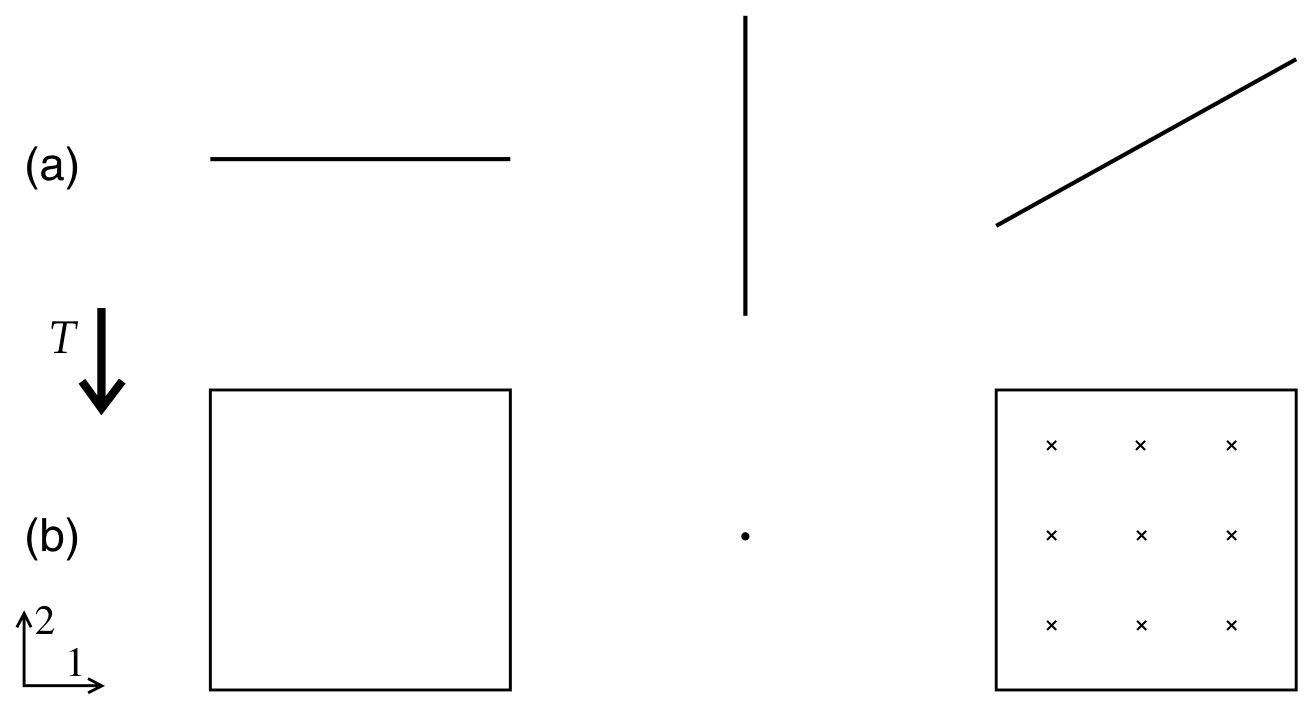
\includegraphics[width=0.75\textwidth]{figure/Fig13.2.jpg}
	\caption{Effect of a T-duality in the 2-direction on D1-branes at various angles in the $(1,2)$ plane: (a) before T-duality; (b) after T-duality. The $\times$s indicate a magnetic field on the D2-brane.}
	\label{fig:13.2}
\end{figure}

The IIB theory also has a 0-form potential $C_{\textit{0}}$, the R--R scalar. This should couple to a `($-1$)-brane.' Indeed, there is a natural interpretation to this: it is defined by Dirichlet boundary conditions in all directions, time as well as space, so its worldsheet is zero-dimensional and the integral \eqref{13.2.7} reduces to the value of $C_{\textit{0}}$ at that point. An object that is localized in time as well as space is an instanton. Instantons in Euclidean path integrals correspond to tunneling events, and these must be present in string theory.

We will verify the R--R couplings of D-branes in the next section; for the remainder of this section we will discuss some of the consequences. The discovery that D-branes carry R--R charges neatly ties together two loose ends. On the one hand, it was argued in section 12.1 that the ordinary string states do not have R--R charges, but now we see that string theory does have a source for every gauge field. This extends the result from chapter 8, that the gauge field from compactification of the antisymmetric tensor couples to winding strings. On the other hand, the existence of so many different kinds of extended object, D$p$-branes for every $p$, might have seemed excessive, but we now see that these are in one-to-one correspondence with the R--R potentials of the respective Type II theories.

The divergence of the Type I theory for groups other than $\mathrm{SO}(32)$ arose from the R--R 10-form field equation. This divergence is unaffected by toroidal compactification and again cancels only for $\mathrm{SO}(32)$. It would have been surprising if toroidal compactification made a consistent theory inconsistent, or the reverse, and it is not hard to verify explicitly that this does not happen. The effect of toroidal compactification is to add worldsheets that wrap around the periodic directions of spacetime. These correspond to exchange of closed strings with winding number, which are massive and so do not have dangerous tadpoles.

The spacetime interpretation of the divergence in the T-dual picture with D-branes is again an inconsistency in the R--R field equations. One can picture field lines emerging from each D-brane, orthogonal to the noncompact dimensions, and these field lines must end somewhere. Further, all D-branes must have the same sign of the charge: the full set of D-branes is still a BPS state, being T-dual to the Type I theory, and the total mass is linear in the total charge for a BPS state. We know that the disk tadpole is canceled by the unoriented cross-cap. In the T-dual spacetime the cross-cap must be localized near one of the orientifold planes, because the string theory in the bulk is oriented. Thus we deduce that the orientifold planes are sinks for R--R charge. If we T-dualize on $k$ dimensions there are $2^k$ orientifold planes but still 16 D-branes, so the charge of an orientifold plane must be $-2^{4-k}$ times that of a D-brane of the same dimension.
\begin{tcolorbox}[breakable]
	\begin{remark}
		\textbf{Conventions.} Charges are counted on the quotient space $T^k/\mathbb Z_2$, where a D-brane and its image count as one object; this is how the text counts ``16 D-branes''. On the covering torus there are 32 branes (16 plus images) and each O-plane appears once.

		Gauss's law on the compact transverse space says the total R--R charge must vanish, since the flux lines have nowhere to go. With D-brane charge $\mu$ and O-plane charge $\mu_{\rm O}$, the $2^k$ fixed planes of $T^k/\mathbb Z_2$ give
		\begin{align*}
			0 = 16\,\mu + 2^k\,\mu_{\rm O} \;\Longrightarrow\; \mu_{\rm O} = -\frac{16}{2^k}\,\mu = -2^{4-k}\,\mu .
		\end{align*}
		The $2^k$ counts the fixed points of $x^m\to-x^m$ on $T^k$: in each circle direction the fixed points are $x^m=0$ and $x^m=\pi R'$, so there are $2$ per direction. For $k=1$ this gives two O8-planes of charge $-8$ each, balancing 16 D8-branes, and for $k=6$ it gives 64 O3-planes of charge $-\frac14$. Counted on the covering space the same statement reads $32\mu+2^k\mu'_{\rm O}=0$ with $\mu'_{\rm O}=-2^{5-k}\mu$. This is the same $-2^{5-k}$ that the text quotes for the D-brane/O-plane force after \eqref{13.3.7}, where it is explained as the flux of the O-plane being squeezed into half the solid angle.
	\end{remark}
\end{tcolorbox}

\subsection*{New Connections Between String Theories}

Starting from the toroidally compactified Type I theory, we can reach either $d = 10$ Type II theory. Simply take an odd or even number of radii to zero, while moving the D-branes and fixed planes off to infinity as the dual spacetime expands. Thus, just as for the two heterotic theories, these should be thought of as limits of a single theory. The theory has many other states as well: we can take the limit while keeping some of the D-branes in fixed positions, so that we obtain the compact theory in a state with D-branes. The simple T-duality leads only to parallel D-branes of equal dimension, but since the D-branes are dynamical we can continuously vary their configurations. We can then reach states with $p$-branes of different dimension as follows. Consider two D1-branes (D-strings) in the IIB theory, from dualizing in eight directions. Let one be along the 1-direction and the other be rotated to lie along the 2-direction. As illustrated in Figure~\ref{fig:13.2}, a further T-duality in the 2-direction reverses Dirichlet and Neumann boundary conditions in this direction and so turns the first D-string into a D2-brane extended in the 1- and 2-directions but the second into a D0-brane. Thus these can coexist in the IIA theory. Of course T-duality leads only to states with 16 D-branes, but we understand now that this is due to the R--R flux conservation in the compact space. In a noncompact space the R--R flux can run to infinity and so any number of D-branes should be allowed.

Thus, starting from the Type I theory we can reach states that look like the Type IIA theory with any collection of even D$p$-branes or the Type IIB theory with any collection of odd D$p$-branes. Of course if we start with an ordinary Type II theory, T-duality will never give us open strings or D-branes, so one might imagine that there is a different Type II theory in which D-branes are not allowed. This seems unlikely, however: everything we know points to the uniqueness of the theory, so we do not have such alternatives. Also, we will see in the next chapter that the inclusion of D-branes leads to a much more elegant and symmetric theory.

In summary, we are now considering a single theory, which has a state that contains no D-branes and looks like the ordinary IIA theory, a second state (T-dual to the first) that contains no D-branes and looks like the ordinary IIB theory, and a third state that contains 16 D9-branes (and an orientifold 9-plane) that looks like the Type I theory. It also contains an infinite number of other states with very general configurations of D-branes.

We can now write down the supersymmetry algebra for this theory:
\begin{subequations} \label{13.2.9}
	\begin{align}
		\{Q_\alpha, Q_\beta\} &= 2(\mathcal{C}\Gamma_\mu)_{\alpha\beta}\bigl(P^\mu + (2\pi\alpha')^{-1}Q_{\mathrm{NS}}^\mu\bigr) \:, \label{13.2.9a} \\
		\{\tilde{Q}_\alpha, \tilde{Q}_\beta\} &= 2(\mathcal{C}\Gamma_\mu)_{\alpha\beta}\bigl(P^\mu - (2\pi\alpha')^{-1}Q_{\mathrm{NS}}^\mu\bigr) \:, \label{13.2.9b} \\
		\{Q_\alpha, \tilde{Q}_\beta\} &= 2\sum_{p}\frac{\tau_p}{p!}Q_{\mathrm{R}}^{\mu_1\dots\mu_p}(\mathcal{C}\beta_{\mu_1}\cdots\beta_{\mu_p})_{\alpha\beta} \:. \label{13.2.9c}
	\end{align}
\end{subequations}
The spacetime supersymmetries $Q_\alpha$ and $\tilde{Q}_\alpha$ act respectively on the left- and right-movers. The anticommutator \eqref{13.2.9b} of two right-moving supersymmetries is the same as the heterotic string anticommutator \eqref{11.6.32}, containing the charge that couples to the NS--NS 2-form. The argument for the appearance of this term is the same as before: the $\tilde{V}_\alpha\tilde{V}_\beta$ OPE contains the right-moving momentum $\bar{\del}X^\mu$, which involves both ordinary momentum and winding number. Similarly, the $V_\alpha V_\beta$ OPE contains the left-moving momentum $\del X^\mu$, so the NS--NS charge appears in the left-moving anticommutator with the opposite sign. We have added a superscript NS to distinguish this charge from the charges $Q_{\mathrm{R}}$ that couple to R--R forms. Also, we have changed conventions so that all charges are now normalized to one per unit worldvolume of the respective extended object, and so the string tension $(2\pi\alpha')^{-1}$ appears explicitly. As discussed in section 11.6, $Q_{\mathrm{NS}}^\mu$ is the charge carried by the fundamental string, meaning the original quantized string. Henceforth we use this term, or F-string, to distinguish it from the D1-brane.

From the argument that D-branes are BPS states, we expect the R--R charges to appear in the algebra as well, and the natural place for an R--R charge to appear is in the anticommutator of a left- and a right-moving supersymmetry. The sum on $p$ runs over even values in the IIA theory and odd values in the IIB theory. By analogy with the NS--NS case we have included the D-brane tensions $\tau_p$, whose values will be obtained in the next section; the factor of $1/p!$ offsets the sum over permutations of indices. To see that the algebra is correct, focus on a state that contains a single static D$p$-brane. The nonzero charge is $Q_{\mathrm{R}}^{\mu_1\dots\mu_p}$, where the indices run over the directions tangent to the D$p$-brane. Note that
\begin{equation}
	\beta_{\mu_1}\cdots\beta_{\mu_p} = \beta_\perp\Gamma^0 \:, \label{13.2.10}
\end{equation}
up to a possible overall sign that can be reabsorbed in the definition of $\tilde{Q}$; $\beta_\perp$ is the same as in equation \eqref{13.2.5}. It then follows that the anticommutator of $Q + \beta_\perp\tilde{Q}$ with any supercharge vanishes in this state, as required by the BPS property. (In equation \eqref{13.2.5} we included primes on the supercharges to indicate that we were working in a T-dual description to the Type I theory with which we began. In writing the algebra \eqref{13.2.9} we are considering an arbitrary state with D-branes, without necessarily obtaining it from T-duality, so there are no primes.)

Incidentally, the central charge \eqref{13.2.9} is still not complete: the magnetic NS--NS charge is missing. This is not carried by D-branes or F-strings. We will discuss this further in the next chapter.

Finally, let us also explain the necessity of D-instantons, localized in time. We could try to use T-duality in the time direction, but it is not clear whether this is meaningful. Rather, consider D0-branes, whose worldlines are one-dimensional, in a space with one compact spatial dimension. For an ordinary quantized particle in a path sum description we would have to include closed paths that wind around the compact direction. Such paths are responsible for Casimir energies and other effects of compactification. Presumably we must do the same for the D0-branes as well. The shortest such winding path is a straight line in the compact spatial direction. This is localized in time and so is essentially an instanton: Casimir energies, in the path sum description, are essentially instanton effects. Further, by a T-duality in the compact dimension we obtain a D-instanton that is localized in all directions. We know from chapter 8 that the D-brane action depends on the closed string coupling as $\mathcal{O}(1/g)$, so the D-instanton amplitude is of order $\me^{-\mathcal{O}(1/g)}$. Thus we have found an example of the enhanced nonperturbative effects that were inferred in section 9.7 from the high order behavior of string perturbation theory.

On the heterotic worldsheet there are no boundary conditions that preserve the worldsheet gauge symmetries, and there is no indication that D-branes exist. Nevertheless, we will see in the next chapter that the D-branes of the Type I/II theory enable us to learn a great deal about the heterotic string as well.


\section{The D-Brane Charge and Action}

There is no force between static BPS objects of like charge. The multi-object state is still supersymmetric and so its energy is determined only by its charge and is independent of the separations. For parallel D$p$-branes, the unbroken supersymmetry \eqref{13.2.5} is the same as for a single D$p$-brane. The vanishing of the force comes about from a cancellation between attraction due to the graviton and dilaton and repulsion due to the R--R tensor. We can calculate these forces explicitly from the usual cylinder vacuum amplitude. The exchange of light NS--NS closed strings was isolated in \eqref{10.8.4}. Modify this expression by removing the factors for the momentum integrations in the Dirichlet directions and introducing a term for the tension of a string stretched over a separation $y^\mu$:
\begin{align}
	\mathcal{A}_{\mathrm{NS-NS}} &\approx \mi V_{p+1}\frac{4\times 16}{8\pi(8\pi^2\alpha')^5}\int_0^\infty \frac{\pi\dif t}{t^2}\,(8\pi^2\alpha' t)^{(9-p)/2}\exp\Bigl(-\frac{t y^2}{2\pi\alpha'}\Bigr) \nonumber \\
	&= \mi V_{p+1} 2\pi(4\pi^2\alpha')^{3-p}G_{9-p}(y) \label{13.3.1}
\end{align}
with $G_d(y) = 2^{-2}\pi^{-d/2}\Gamma(\frac{1}{2}d - 1)y^{2-d}$ the scalar Green's function. The Chan--Paton weight is 2 here, from the two orientations of the open string, and there is no factor of $1/2$ from the orientation projection because the physics is locally oriented.
\begin{tcolorbox}[breakable]
	\begin{remark}
		\textbf{Conventions.} The prefactor $4\times16/[8\pi(8\pi^2\alpha')^5]$ and the measure $\pi\,\dif t/t^2$ are taken from the large-$t$ (closed-string) limit of the cylinder, \eqref{10.8.4}, with the Chan--Paton weight 2 included. $t$ is the open-string modulus, so each open-string state is weighted by $e^{-2\pi tL_0}$ with $L_0=\alpha'(k^2+m^2)+\dots$.

		\textit{Origin of the two modifications.} The momentum integral runs only over the $p+1$ Neumann directions, and a string stretched across the separation $y$ has an extra mass term $L_0\supset\alpha'(y/2\pi\alpha')^2$:
		\begin{align*}
			\int\frac{\dif^{p+1}k}{(2\pi)^{p+1}}\,e^{-2\pi t\alpha'k^2} \eqs{1} (8\pi^2\alpha't)^{-(p+1)/2} = (8\pi^2\alpha't)^{-5}\,(8\pi^2\alpha't)^{(9-p)/2},\\
			e^{-2\pi t\alpha'(y/2\pi\alpha')^2} = \exp\Bigl(-\frac{ty^2}{2\pi\alpha'}\Bigr).
		\end{align*}
		At (1), each Gaussian gives $(2\pi)^{-1}(\pi/2\pi t\alpha')^{1/2}=(8\pi^2\alpha't)^{-1/2}$. The first factor is the ten-dimensional one of \eqref{10.8.4} (together with $V_{10}\to V_{p+1}$), so the rest is the factor $(8\pi^2\alpha't)^{(9-p)/2}$ in \eqref{13.3.1}.

		\textit{The $t$ integral.} With $u=ty^2/2\pi\alpha'$,
		\begin{align*}
			\int_0^\infty \frac{\pi\,\dif t}{t^2}(8\pi^2\alpha't)^{(9-p)/2}e^{-ty^2/2\pi\alpha'}
			&\eqs{2} \pi(8\pi^2\alpha')^{(9-p)/2}\Bigl(\frac{2\pi\alpha'}{y^2}\Bigr)^{(7-p)/2}\Gamma\Bigl(\frac{7-p}{2}\Bigr)\\
			&\eqs{3} \pi(8\pi^2\alpha')^{(9-p)/2}(2\pi\alpha')^{(7-p)/2}\cdot 4\pi^{(9-p)/2}\,G_{9-p}(y) .
		\end{align*}
		At (2), $\int_0^\infty\dif t\,t^{s-1}e^{-at}=a^{-s}\Gamma(s)$ with $s=(7-p)/2$. At (3), $G_{9-p}(y)=\frac14\pi^{-(9-p)/2}\Gamma(\frac{7-p}{2})y^{p-7}$, since $\frac12 d-1=\frac{7-p}{2}$ and $y^{2-d}=y^{p-7}$ for $d=9-p$. Multiplying by the prefactor,
		\begin{align*}
			\frac{\mathcal A_{\rm NS-NS}}{\mi V_{p+1}G_{9-p}(y)} &= \frac{64\,\pi}{8\pi}\cdot4\,(8\pi^2\alpha')^{-(p+1)/2}(2\pi\alpha')^{(7-p)/2}\pi^{(9-p)/2}\\
			&\eqs{4} 2^{7-2p}\pi^{7-2p}{\alpha'}^{3-p} = 2\pi(4\pi^2\alpha')^{3-p} .
		\end{align*}
		At (4) the exponents were collected: for $\alpha'$, $\frac{7-p}{2}-\frac{p+1}{2}=3-p$; for $\pi$, $-(p+1)+\frac{7-p}{2}+\frac{9-p}{2}=7-2p$; for 2, $5-\frac{3(p+1)}{2}+\frac{7-p}{2}=7-2p$. This is the second line of \eqref{13.3.1}.
	\end{remark}
\end{tcolorbox} Due to supersymmetric cancellation in the trace, the R--R exchange amplitude is
\begin{equation}
	\mathcal{A}_{\mathrm{R-R}} = -\mathcal{A}_{\mathrm{NS-NS}} \label{13.3.2}
\end{equation}
and so the total force vanishes as expected.
\begin{tcolorbox}[breakable]
	\begin{remark}
		\textbf{Conventions.} As in section 10.8, the open-string trace over the $p$-$p$ strings on the cylinder is proportional to
		\begin{equation*}
			Z_{00}(\mi t)^4-Z_{01}(\mi t)^4-Z_{10}(\mi t)^4 \ (-Z_{11}^4=0),
		\end{equation*}
		with the terms being, respectively, the NS trace, the NS trace with $(-1)^F$, and the R trace. Under $t\to1/t$ (the closed-string channel), $Z_{00}\to Z_{00}$ and $Z_{01}\leftrightarrow Z_{10}$ up to common factors, by the modular properties \eqref{10.7.14}.

		\textit{Which terms are which exchange.} In the closed channel, a closed-string state propagating between the boundaries is NS--NS if the world-sheet fermions are antiperiodic around the closed-string circle, which is the open-string time direction. That is the case for the open-string traces without the $(-1)^F$ insertion, $Z_{00}^4$ and $Z_{10}^4$; the R--R exchange is the trace with $(-1)^F$ in the NS sector, $Z_{01}^4$. The GSO sign structure gives
		\begin{equation*}
			\mathcal A_{\rm NS-NS}\propto Z_{00}^4-Z_{10}^4,\qquad \mathcal A_{\rm R-R}\propto -Z_{01}^4 ,
		\end{equation*}
		with the same proportionality constant. The abstruse identity \eqref{7.2.41}, $Z_{00}^4-Z_{01}^4-Z_{10}^4=0$, then says $\mathcal A_{\rm NS-NS}=Z_{01}^4\times(\cdots)=-\mathcal A_{\rm R-R}$ at every $t$, not only for the massless exchange, which is \eqref{13.3.2}.
	\end{remark}
\end{tcolorbox}

The field theory calculation \eqref{8.7.25} for the dilaton--graviton potential changes only by the substitution $6 = (D-2)/4 \to 2$, and so is
\begin{equation}
	2\mi\kappa_{10}^2\tau_p^2\,G_{9-p}(y) \:. \label{13.3.3}
\end{equation}
Thus
\begin{equation}
	\tau_p^2 = \frac{\pi}{\kappa_{10}^2}(4\pi^2\alpha')^{3-p} \:. \label{13.3.4}
\end{equation}
This satisfies the same T-duality relation as in the bosonic string.
\begin{tcolorbox}[breakable]
	\begin{remark}
		\textbf{Conventions.} We use the Einstein-frame action of section 8.7 in $D$ dimensions, $\frac{1}{2\kappa^2}\int\dif^Dx\,(-G_{\rm E})^{1/2}\bigl(R-\frac{4}{D-2}\partial_\mu\tilde\Phi\partial^\mu\tilde\Phi\bigr)$ with $\tilde\Phi=\Phi-\Phi_0$. Here $\kappa=\kappa_{10}e^{\Phi_0}$ is the physical gravitational coupling, and the brane action is $-T_p\int e^{-\Phi}(-\det G_{\rm s})^{1/2}$ with $\tau_p=T_pe^{-\Phi_0}$ and $G_{\rm s}=e^{4\tilde\Phi/(D-2)}G_{\rm E}$. For the normalization of an exchange, a canonical scalar $-\frac12(\partial\varphi)^2$ with source coupling $g\varphi$ gives amplitude $\mi g^2G$; in the same normalization the graviton gives $\mi\kappa^2\bigl[T^{\mu\nu}T'_{\mu\nu}-\frac{1}{D-2}TT'\bigr]G$. The Newtonian limit in $D=4$ checks this relative factor: it reproduces $-GMM'/r$ with $8\pi G=\kappa^2$.

		\textit{Graviton.} For a static brane $T^{ab}=-\tau_p\eta^{ab}$ along the $p+1$ worldvolume directions, so
		\begin{align*}
			T^{\mu\nu}T_{\mu\nu}-\frac{T^2}{D-2} = \tau_p^2\Bigl[(p+1)-\frac{(p+1)^2}{D-2}\Bigr] = \tau_p^2\,\frac{(p+1)(D-3-p)}{D-2} .
		\end{align*}
		\textit{Dilaton.} In Einstein frame, $e^{-\Phi}(-\det G_{\rm s})^{1/2}=e^{-\Phi_0}e^{a\tilde\Phi}(-\det G_{\rm E})^{1/2}$ with $a=-1+\frac{2(p+1)}{D-2}=\frac{2p+4-D}{D-2}$, so the brane couples as $-\tau_pa\tilde\Phi$. The canonical field is $\varphi=\tilde\Phi\,[4/(\kappa^2(D-2))]^{1/2}$, so $g^2=\tau_p^2a^2\kappa^2(D-2)/4$. Adding,
		\begin{align*}
			\frac{\mathcal A}{\mi\kappa^2\tau_p^2G} &= \frac{(p+1)(D-3-p)}{D-2} + \frac{(2p+4-D)^2}{4(D-2)}\\
			&\eqs{1} \frac{1}{D-2}\Bigl[q(D-2)-q^2 + q^2 - q(D-2) + \tfrac14(D-2)^2\Bigr] = \frac{D-2}{4} .
		\end{align*}
		At (1), $q=p+1$ was substituted, so $2p+4-D=2q-(D-2)$ and $(p+1)(D-3-p)=q(D-2)-q^2$. The $p$-dependence cancels between graviton and dilaton. For $D=26$ this is the $6$ of \eqref{8.7.25}, and for $D=10$ it is $2$, giving $2\mi\kappa^2\tau_p^2G_{9-p}$, which is \eqref{13.3.3} per unit worldvolume.

		Equating to the NS--NS part of the string amplitude \eqref{13.3.1}, per unit $V_{p+1}$,
		\begin{equation*}
			2\pi(4\pi^2\alpha')^{3-p} = 2\kappa^2\tau_p^2 \;\Longrightarrow\; \tau_p^2=\frac{\pi}{\kappa^2}(4\pi^2\alpha')^{3-p},
			\qquad \frac{\tau_{p-1}^2}{\tau_p^2}=4\pi^2\alpha' ,
		\end{equation*}
		which is \eqref{13.3.4} and the T-duality relation $\tau_{p-1}=2\pi\alpha'^{1/2}\tau_p$ (for $R=\alpha'^{1/2}$) found in the bosonic string.

		\textit{Which $\kappa$.} The graviton and dilaton couple through the physical $\kappa=\kappa_{10}e^{\Phi_0}$, so \eqref{13.3.3}--\eqref{13.3.4} should be read with $\kappa$ rather than $\kappa_{10}$. With $\kappa_{10}$ they would give $\tau_p=\mu_p$, contradicting \eqref{13.3.7}, $\mu_p^2=e^{2\Phi_0}\tau_p^2$, for $\Phi_0\neq0$.
	\end{remark}
\end{tcolorbox}
\noindent For the R--R exchange, the low-energy action is
\begin{equation}
	-\frac{1}{4\kappa_{10}^2}\int \dif^{10}x\,(-G)^{1/2}|F_{p+2}|^2 + \mu_p \int C_{p+1} \:. \label{13.3.5}
\end{equation}
The kinetic term is canonically normalized, so the propagator for any given component (such as the one parallel to the D-brane) is $2\kappa_{10}^2\mi/k^2$, and the field theory amplitude is
\begin{equation}
	-2\kappa_{10}^2\mi\mu_p^2\,G_{9-p}(y) \:. \label{13.3.6}
\end{equation}
Hence
\begin{equation}
	\mu_p^2 = \frac{\pi}{\kappa_{10}^2}(4\pi^2\alpha')^{3-p} = \me^{2\Phi_0}\tau_p^2 = T_p^2 \:. \label{13.3.7}
\end{equation}
\begin{tcolorbox}[breakable]
	\begin{remark}
		\textbf{Conventions.} $|F_{p+2}|^2=\frac{1}{(p+2)!}F_{\mu_1\dots\mu_{p+2}}F^{\mu_1\dots\mu_{p+2}}$ as in section 12.1. The R--R kinetic term in \eqref{13.3.5} has no dilaton factor, so its coupling is $\kappa_{10}$. Exchange amplitudes are normalized as in the previous box: a canonical scalar with source $g\varphi$ gives $\mi g^2G$.

		The brane sources the component $C\equiv C_{01\cdots p}$, and for a static configuration only the transverse gradients $\partial_mC$ matter:
		\begin{align*}
			-\frac{1}{4\kappa_{10}^2}|F_{p+2}|^2 &\eqs{1} -\frac{1}{4\kappa_{10}^2}\sum_m F_{m01\cdots p}F^{m01\cdots p}
			\eqs{2} +\frac{1}{4\kappa_{10}^2}(\partial_mC)^2 ,\\
			C=\sqrt2\,\kappa_{10}\,\varphi \;&\Longrightarrow\; \mu_p\!\int C_{p+1} = \sqrt2\,\kappa_{10}\mu_p\!\int\dif^{p+1}\xi\,\varphi .
		\end{align*}
		At (1), each unordered index set appears $(p+2)!$ times in the sum, cancelling the $1/(p+2)!$, and only sets of the form $\{m,0,1,\dots,p\}$ are nonzero. At (2), raising the index 0 costs $\eta^{00}=-1$. So the static field has the opposite sign of kinetic term to an ordinary scalar, exactly like $A_0$ in electrostatics. Its magnitude is canonical for $\varphi=C/\sqrt2\kappa_{10}$, which is the propagator $2\kappa_{10}^2\mi/k^2$ quoted in the text. The flipped sign makes like charges repel:
		\begin{equation*}
			\mathcal A_{\rm R-R}^{\rm field} = -\mi\bigl(\sqrt2\kappa_{10}\mu_p\bigr)^2G_{9-p} = -2\mi\kappa_{10}^2\mu_p^2\,G_{9-p},
		\end{equation*}
		which is \eqref{13.3.6}. Matching with $\mathcal A_{\rm R-R}=-\mathcal A_{\rm NS-NS}$, \eqref{13.3.2}, and \eqref{13.3.1} per unit volume,
		\begin{align*}
			2\kappa_{10}^2\mu_p^2 = 2\pi(4\pi^2\alpha')^{3-p} \;\Longrightarrow\; \mu_p^2=\frac{\pi}{\kappa_{10}^2}(4\pi^2\alpha')^{3-p} \eqs{3} \frac{\kappa^2}{\kappa_{10}^2}\tau_p^2 \eqs{4} e^{2\Phi_0}\tau_p^2 = T_p^2 .
		\end{align*}
		At (3), \eqref{13.3.4} with the physical $\kappa$ was used. At (4), $\kappa=\kappa_{10}e^{\Phi_0}$, and $T_p=e^{\Phi_0}\tau_p$ is the tension without the $1/g$ of the string-frame action. The cancellation between attraction ($2\kappa^2\tau_p^2$) and repulsion ($2\kappa_{10}^2\mu_p^2$) is therefore the statement $\kappa\tau_p=\kappa_{10}\mu_p$: tension and charge are in the BPS ratio, as the algebra \eqref{bps} requires.
	\end{remark}
\end{tcolorbox}

The reader can carry out a similar calculation of the force between a D-brane and an orientifold plane and show that it has an additional $-2^{5-k}$. We deduced from the cancellation of divergences that the charge of the orientifold plane should have a factor of $-2^{4-k}$; the extra factor of 2 in the force arises because the orientifold geometry squeezes the flux lines into half the solid angle.

The calculation of the interaction confirms our earlier deduction that D-branes carry the R--R charges. It is interesting to see how this is consistent with our earlier discussion of string vertex operators. The R--R vertex operator \eqref{12.1.14} is in the $(-1/2, -1/2)$ picture, which can be used in almost all processes. On the disk, however, the total left- plus right-moving ghost number must be $-2$. With two or more R--R vertex operators, all can be in the $(-1/2, -1/2)$ picture (with PCOs included as well), but a single vertex operator must be in either the $(-3/2, -1/2)$ or the $(-1/2, -3/2)$ picture. The $(-1/2, -1/2)$ vertex operator is essentially $\me^{-\phi}G_0$ times the $(-3/2, -1/2)$ operator, so besides the shift in the ghost number the latter has one less power of momentum and one less $\Gamma$-matrix. The missing factor of momentum turns $F$ into $C$, and the missing $\Gamma$-matrix gives the correct Lorentz representations for the potential rather than the field strength.

\subsection*{Dirac Quantization Condition}

There is an important consistency check on the value of the R--R charge, which generalizes the Dirac quantization condition for magnetic monopole charge. Let us review the Dirac condition, shown in Figure~\ref{fig:13.3}. Consider a magnetic charge $\mu_{\mathrm{m}}$ at the origin. The integrated flux is
\begin{equation}
	\int_{S^2} F_{\textit{2}} = \mu_{\mathrm{m}} \:. \label{13.3.8}
\end{equation}
Because the integral over a closed surface is nonzero, we cannot write $F_{\textit{2}} = \dif A_{\textit{1}}$ for any globally well-defined vector potential. However, we can write $F_{\textit{2}} = \dif A_{\textit{1}}$ except along a Dirac string ending on the monopole. Now consider an electric charge $\mu_{\mathrm{e}}$ moving in this field. Its coupling to the field produces a phase
\begin{equation}
	\exp\Bigl(\mi\mu_{\mathrm{e}}\int_P A_{\textit{1}}\Bigr) = \exp\Bigl(\mi\mu_{\mathrm{e}}\int_D F_{\textit{2}}\Bigr) \label{13.3.9}
\end{equation}
when the particle moves on a closed path $P$. The surface $D$ spans $P$ and does not intersect the Dirac string. Now consider the limit as the path is contracted to a small circle around the Dirac string. The phase becomes
\begin{equation}
	\exp\Bigl(\mi\mu_{\mathrm{e}}\int_{S^2} F_{\textit{2}}\Bigr) = \exp(\mi\mu_{\mathrm{e}}\mu_{\mathrm{m}}) \:. \label{13.3.10}
\end{equation}
The Dirac string must be invisible, so this phase must be 1. Equivalently, this is the condition that the phase \eqref{13.3.9} is unchanged if we replace $D$ with a surface $D'$ that passes on the other side of the monopole, so $D - D' = S^2$. The condition is
\begin{equation}
	\mu_{\mathrm{e}}\mu_{\mathrm{m}} = 2\pi n \label{13.3.11}
\end{equation}
with $n$ an integer.

\begin{figure}[htbp]
	\centering
	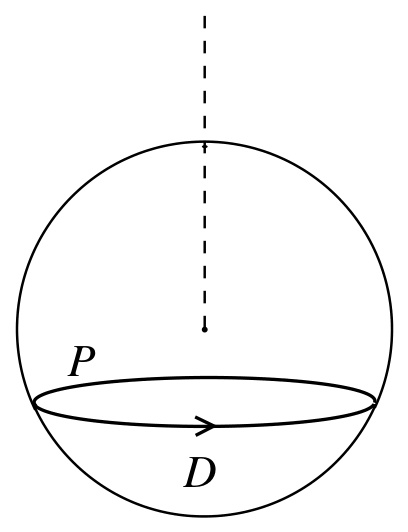
\includegraphics[width=0.35\textwidth]{figure/Fig13.3.jpg}
	\caption{Sphere surrounding monopole, with a Dirac string running upward. The particle path $P$ is bounded by the lower cap $D$.}
	\label{fig:13.3}
\end{figure}

The Dirac condition generalizes directly to extended objects and their charges. Let us think about $F_{p+2}$ as the field strength, so that the $p$-brane is an electric source and the $(6-p)$-brane a magnetic source. In nine dimensions a $(6-p)$-dimensional object is surrounded by a $(p+2)$-sphere, so by analogy to the magnetic flux \eqref{13.3.8},
\begin{equation}
	\int_{S^{p+2}} F_{p+2} = \frac{2\kappa_{10}^2}{\mu_{6-p}} \:. \label{13.3.12}
\end{equation}
One can then repeat the same argument. For example, let the $p$-brane be extended in the directions $4 \le \mu \le p+3$ and the $(6-p)$-brane in the directions $p+4 \le \mu \le 9$. The system essentially reduces to the three-dimensional situation of Figure~\ref{fig:13.3} in the directions $\mu = 1, 2, 3$, and the charges must satisfy
\begin{equation}
	2\kappa_{10}^2\mu_p\mu_{6-p} = 2\pi n \:. \label{13.3.13}
\end{equation}
Remarkably, the charges \eqref{13.3.7}, arrived at in an entirely different way, satisfy this relation with the minimum quantum $n = 1$.
\begin{tcolorbox}[breakable]
	\begin{remark}
		\textbf{Conventions.} The $(6-p)$-brane is an electric source for $C_{7-p}$, with action $-\frac{1}{4\kappa_{10}^2}\int F_{8-p}\wedge*F_{8-p}+\mu_{6-p}\int C_{7-p}$. Here $\int\dif^{10}x\,(-G)^{1/2}|F|^2=\int F\wedge*F$, and $F_{p+2}=\pm*F_{8-p}$ describes the same field. Overall orientation signs are dropped; only magnitudes enter the Dirac condition.

		\textit{Flux of the magnetic source.} Varying $C_{7-p}$,
		\begin{align*}
			0=\delta S &= -\frac{1}{2\kappa_{10}^2}\int \dif\,\delta C_{7-p}\wedge*F_{8-p} + \mu_{6-p}\int_{\mathcal W}\delta C_{7-p}\\
			&\eqs{1} \pm\frac{1}{2\kappa_{10}^2}\int\delta C_{7-p}\wedge\dif*F_{8-p} + \mu_{6-p}\int\delta C_{7-p}\wedge\delta_{\mathcal W} ,\\
			\int_{S^{p+2}}F_{p+2} &\eqs{2} \pm\int_{S^{p+2}}*F_{8-p} \eqs{3} \pm\int_{B^{p+3}}\dif*F_{8-p}\\
			&= 2\kappa_{10}^2\,\mu_{6-p} .
		\end{align*}
		At (1), integration by parts, with $\delta_{\mathcal W}$ the $(p+3)$-form delta function transverse to the worldvolume. At (2), $F_{p+2}=\pm*F_{8-p}$. At (3), Stokes's theorem on the ball whose boundary is the $(p+2)$-sphere around the $(6-p)$-brane, and the field equation $\dif*F_{8-p}=\pm2\kappa_{10}^2\mu_{6-p}\delta_{\mathcal W}$. So the flux is $2\kappa_{10}^2\mu_{6-p}$, not $2\kappa_{10}^2/\mu_{6-p}$ as printed in \eqref{13.3.12}. With this flux, the Dirac argument \eqref{13.3.9}--\eqref{13.3.11} with $\mu_{\rm e}=\mu_p$ and $\mu_{\rm m}=2\kappa_{10}^2\mu_{6-p}$ gives \eqref{13.3.13} as printed. The printed \eqref{13.3.12} would instead give $2\kappa_{10}^2\mu_p/\mu_{6-p}=2\pi n$, which is not symmetric between the two branes.

		\textit{Check with \eqref{13.3.7}.}
		\begin{align*}
			\mu_p^2\mu_{6-p}^2 = \frac{\pi^2}{\kappa_{10}^4}(4\pi^2\alpha')^{3-p}(4\pi^2\alpha')^{3-(6-p)} \eqs{4} \frac{\pi^2}{\kappa_{10}^4}
			\;\Longrightarrow\; 2\kappa_{10}^2\mu_p\mu_{6-p} = 2\pi .
		\end{align*}
		At (4), the exponents $3-p$ and $p-3$ cancel, so $\alpha'$ drops out. The minimal quantum $n=1$ is saturated for every $p$.
	\end{remark}
\end{tcolorbox}

\subsection*{D-Brane Actions}

The coupling of a D-brane to NS--NS closed string fields is the same Dirac--Born--Infeld action as in the bosonic string:
\begin{equation}
	S_{\mathrm{D}p} = -\mu_p\int \dif^{p+1}\xi\,\operatorname{Tr}\Bigl(\me^{-\Phi}\bigl[-\det(G_{ab} + B_{ab} + 2\pi\alpha' F_{ab})\bigr]^{1/2}\Bigr) \:, \label{13.3.14}
\end{equation}
where $G_{ab}$ and $B_{ab}$ are the components of the spacetime NS--NS fields parallel to the brane and $F_{ab}$ is the gauge field living on the brane. The argument leading to this form is exactly as in the bosonic case, section 8.7. Recall that for $n$ D-branes at small separation, where the strings stretched between them are light enough to be included in the low energy action, the collective coordinates $X^\mu(\xi)$, gauge fields $A_a(\xi)$, and their fermionic partners $\lambda(\xi)$ all become $n \times n$ matrices. The trace in the action is in this $n \times n$ space. In addition there is a term
\begin{equation}
	\mathcal{O}([X^m, X^n]^2) \label{13.3.15}
\end{equation}
in the potential. As discussed in chapter 8, the effect of this potential is that in the flat directions the collective coordinates become diagonal. They can then be interpreted as $n$ ordinary collective coordinates for $n$ objects. At small separation the full matrix dynamics is crucial, as we will see.

The coupling to the R--R background also includes corrections involving the gauge field on the brane. Like the Born--Infeld action, these can be deduced via T-duality. Consider, as an example, a 1-brane in the $(1,2)$ plane. The action is
\begin{equation}
	\int C_{\textit{2}} = \int \dif x^0(\dif x^1 C_{01} + \dif x^2 C_{02}) = \int \dif x^0\dif x^1\bigl(C_{01} + \del_1 X^2 C_{02}\bigr) \:. \label{13.3.16}
\end{equation}
Under a T-duality in the 2-direction this becomes:
\begin{equation}
	\int \dif x^0\dif x^1\bigl(C_{012} + 2\pi\alpha' F_{12}C_0\bigr) \:. \label{13.3.17}
\end{equation}
We have used the T-transformation of the $C$ fields, \eqref{13.1.5}. A D-brane at an angle is T-dual to one with a magnetic field, as in Figure~\ref{fig:13.2}. We are not keeping track of the normalization but one could, with the result $\mu_p = \mu_{p-1}/(2\pi{\alpha'}^{1/2})$ in agreement with the explicit calculation. The generalization of \eqref{13.3.17} to an arbitrary configuration, and to multiple D-branes, gives the Chern--Simons-like result
\begin{equation}
	\mi\mu_p\int_{\mathcal{W}_{p+1}}\operatorname{Tr}\Bigl[\exp\bigl(2\pi\alpha' F_{\textit{2}} + B_{\textit{2}}\bigr)\wedge \sum_{q}C_q\Bigr] \:. \label{13.3.18}
\end{equation}
The expansion of the integrand \eqref{13.3.18} involves forms of various rank; the integral picks out precisely the terms that are proportional to the volume form of the $p$-brane worldvolume. There are similar couplings with the spacetime curvature in addition to the field strength; these can be obtained from a string calculation:
\[
S_{\mathrm{WZ}} = \mi\mu_p\int_{\mathcal{W}_{p+1}}\operatorname{Tr}\Bigl[\exp\bigl(2\pi\alpha' F_{\textit{2}} + B_{\textit{2}}\bigr)\wedge \sum_{q}C_q\Bigr]\wedge \sqrt{\hat{A}(\mathcal{R})} \:.
\]
\begin{tcolorbox}[breakable]
	\begin{remark}
		\textbf{Conventions.} Static gauge $\xi^a=x^a$ is used, and the transverse position of the D1-brane is $X^2(x^0,x^1)$. The T-duality dictionary of chapter 8 is $X^m=2\pi\alpha'A_m$ for a dualized direction $m$, with fields independent of $x^2$. Signs from \eqref{13.1.5} (``up to signs'') are dropped, as in the text.

		\textit{From \eqref{13.3.16} to \eqref{13.3.17}.} The pullback of $C_2$ to the tilted string is
		\begin{align*}
			\int C_{\textit{2}} &= \int \dif x^0\wedge\bigl(\dif x^1C_{01}+\dif x^2C_{02}\bigr) \eqs{1} \int\dif x^0\dif x^1\bigl(C_{01}+\partial_1X^2\,C_{02}\bigr)\\
			&\eqs{2} \int\dif x^0\dif x^1\bigl(C_{012}+2\pi\alpha'\partial_1A_2\,C_0\bigr) \eqs{3} \int\dif x^0\dif x^1\bigl(C_{012}+2\pi\alpha'F_{12}\,C_0\bigr).
		\end{align*}
		At (1), $\dif x^2=\partial_1X^2\,\dif x^1+\partial_0X^2\,\dif x^0$ on the worldsheet, and the $\dif x^0$ term drops against $\dif x^0$. At (2), \eqref{13.1.5}: $C_{01}$ gains the index 2, $C_{02}$ loses it, and $X^2\to2\pi\alpha'A_2$. At (3), $F_{12}=\partial_1A_2-\partial_2A_1=\partial_1A_2$ because nothing depends on $x^2$. The worldvolume is now the D2-brane along $x^0,x^1,x^2$, and $\int\dif x^2$ gives the dual circle's length, which is where the normalization $\mu_2=\mu_1/(2\pi\alpha'^{1/2})$ enters. From \eqref{13.3.7} in general, $\mu_p/\mu_{p-1}=(4\pi^2\alpha')^{-1/2}=1/(2\pi\alpha'^{1/2})$.

		\textit{Expansion of \eqref{13.3.18}.} For one brane and $B=0$, the $(p+1)$-form part of the integrand is
		\begin{align*}
			\Bigl[e^{2\pi\alpha'F}\wedge\sum_qC_q\Bigr]_{p+1} = C_{p+1} + 2\pi\alpha'F\wedge C_{p-1} + \frac{(2\pi\alpha')^2}{2}F\wedge F\wedge C_{p-3} + \cdots .
		\end{align*}
		For $p=2$ the first two terms are $C_{012}\,\dif x^0\dif x^1\dif x^2$ and $2\pi\alpha'F_{12}C_0\,\dif x^1\wedge\dif x^2\wedge\dif x^0$, reproducing \eqref{13.3.17} up to orientation. The term $\frac12(2\pi\alpha')^2F\wedge F\wedge C_{p-3}$ says that an instanton ($\int F\wedge F\neq0$) on a D$p$-brane carries D$(p-4)$ charge; this is used for the D0--D4 system in section 13.6. The combination $2\pi\alpha'F+B$ is fixed because it is the invariant combination under the NS--NS gauge transformation $\delta B=\dif\zeta$, $\delta A=-\zeta/2\pi\alpha'$.
	\end{remark}
\end{tcolorbox}

Thus far we have given only the action for the bosonic fields on the brane. For the leading fluctuations around a flat D-brane in flat spacetime the fermionic action is of the usual Dirac form:
\begin{equation}
	-\mi\int \dif^{p+1}\xi\,\operatorname{Tr}(\bar{\lambda}\Gamma^a D_a\lambda) \:. \label{13.3.19}
\end{equation}
The full nonlinear supersymmetric form is left to the references.

\subsection*{Coupling Constants}

The ratio of the F-string tension to the D-string tension is
\begin{equation}
	\frac{\tau_{\mathrm{F}1}}{\tau_{\mathrm{D}1}} = \frac{1/(2\pi\alpha')}{\kappa/(4\pi^{5/2}\alpha')} = \frac{\kappa}{8\pi^{7/2}{\alpha'}^2} \:. \label{13.3.20}
\end{equation}
Up to now there has been no natural convention for defining the additive normalization of the dilaton field or the multiplicative normalization of the closed string coupling $g = \me^{\Phi}$. The dimensionless ratio \eqref{13.3.20} is proportional to the closed string coupling, and it turns out to be very convenient to take it as the definition of the coupling:
\begin{equation}
	g = \frac{\tau_{\mathrm{F}1}}{\tau_{\mathrm{D}1}} \:. \label{13.3.21}
\end{equation}
Then the gravitational coupling is
\begin{equation}
	\kappa^2 = \frac{1}{2}(2\pi)^7 g^2 {\alpha'}^4 \label{13.3.22}
\end{equation}
and the D-brane tension is
\begin{equation}
	\tau_p = \frac{1}{g(2\pi)^p{\alpha'}^{(p+1)/2}} = (2\kappa^2)^{-1/2}(2\pi)^{(7-2p)/2}{\alpha'}^{(3-p)/2} \:. \label{13.3.23}
\end{equation}
Also, the constant appearing in the low energy actions of section 12.1 is
\begin{equation}
	\kappa_{10}^2 = \frac{1}{2}(2\pi)^7{\alpha'}^4 \:; \label{13.3.24}
\end{equation}
this differs from the physically measured $\kappa$ because the latter depends on the dilaton background.

Expanding the action \eqref{13.3.14} gives the coupling of the Yang--Mills theory on the D$p$-brane:
\begin{equation}
	g_{\mathrm{D}p}^2 = \frac{1}{(2\pi\alpha')^2\tau_p} = (2\pi)^{p-2}g{\alpha'}^{(p-3)/2} \:. \label{13.3.25}
\end{equation}
Notice that for $p = 3$ this coupling is dimensionless, as expected in a $(3 + 1)$-dimensional gauge theory. For $p < 3$ the coupling has units of length to a negative power, and for $p > 3$ length to a positive power.
\begin{tcolorbox}[breakable]
	\begin{remark}
		\textbf{Conventions.} In this subsection $\kappa=\kappa_{10}e^{\Phi_0}$ is the physical coupling and $\tau_p$ the physical tension of \eqref{13.3.4}, $\tau_p^2=\pi(4\pi^2\alpha')^{3-p}/\kappa^2$. The Yang--Mills normalization is $-\frac{1}{4g^2}\int F_{ab}F^{ab}$ for a $\mathrm U(1)$ factor (then $\operatorname{Tr}_{\rm f}$ for $\mathrm U(n)$, \eqref{13.3.26}).

		\textit{The D-string tension and \eqref{13.3.20}.}
		\begin{align*}
			\tau_{\rm D1}^2 \eqs{1} \frac{\pi}{\kappa^2}(4\pi^2\alpha')^2 = \frac{16\pi^5{\alpha'}^2}{\kappa^2}
			\;\Longrightarrow\; \tau_{\rm D1}=\frac{4\pi^{5/2}\alpha'}{\kappa},\qquad
			\frac{\tau_{\rm F1}}{\tau_{\rm D1}} = \frac{1/(2\pi\alpha')}{4\pi^{5/2}\alpha'/\kappa} = \frac{\kappa}{8\pi^{7/2}{\alpha'}^2} .
		\end{align*}
		At (1), \eqref{13.3.4} was used with $p=1$. The final value in \eqref{13.3.20} is correct, but its middle expression has $\tau_{\rm D1}$ inverted: the denominator should read $4\pi^{5/2}\alpha'/\kappa$, not $\kappa/(4\pi^{5/2}\alpha')$.

		\textit{\eqref{13.3.22}--\eqref{13.3.24}.} With $g=\kappa/(8\pi^{7/2}\alpha'^2)$,
		\begin{align*}
			\kappa^2 &= 64\pi^7g^2{\alpha'}^4 \eqs{2} \tfrac12(2\pi)^7g^2{\alpha'}^4, \qquad \kappa=2^{-1/2}(2\pi)^{7/2}g\,{\alpha'}^2,\\
			\tau_p &= \frac{\pi^{1/2}}{\kappa}(2\pi)^{3-p}{\alpha'}^{(3-p)/2} \eqs{3} \frac{(2\pi)^{1/2}(2\pi)^{3-p}{\alpha'}^{(3-p)/2}}{(2\pi)^{7/2}g{\alpha'}^2} = \frac{1}{g(2\pi)^p{\alpha'}^{(p+1)/2}} ,\\
			\tau_p &\eqs{4} (2\kappa^2)^{-1/2}(2\pi)^{1/2}(2\pi)^{3-p}{\alpha'}^{(3-p)/2} = (2\kappa^2)^{-1/2}(2\pi)^{(7-2p)/2}{\alpha'}^{(3-p)/2},\\
			\kappa_{10}^2 &= \frac{\kappa^2}{g^2} = \tfrac12(2\pi)^7{\alpha'}^4 .
		\end{align*}
		At (2), $(2\pi)^7=128\pi^7$. At (3), $\pi^{1/2}\cdot2^{1/2}=(2\pi)^{1/2}$ and $\kappa$ was substituted. At (4), $\pi^{1/2}/\kappa=(2\pi)^{1/2}/(2\kappa^2)^{1/2}$. The last relation uses $\kappa=\kappa_{10}e^{\Phi_0}$ and $g=e^{\Phi_0}$ in the normalization \eqref{13.3.21}.

		\textit{\eqref{13.3.25}.} Expand \eqref{13.3.14} in flat space with $B=0$, constant dilaton, and one brane. With $M^a{}_b=2\pi\alpha'F^a{}_b$,
		\begin{align*}
			\bigl[-\det(\eta_{ab}+2\pi\alpha'F_{ab})\bigr]^{1/2} &= \det\,^{1/2}(1 + M) \\ &\eqs{5} 1+\tfrac12\operatorname{tr}M-\tfrac14\operatorname{tr}M^2+\tfrac18(\operatorname{tr}M)^2+\cdots\\
			&\eqs{6} 1+\tfrac14(2\pi\alpha')^2F_{ab}F^{ab}+\cdots ,\\
			S_{\rm D\it p} &\supset -\tau_p\frac{(2\pi\alpha')^2}{4}\int\dif^{p+1}\xi\,F_{ab}F^{ab}\\ &\equiv -\frac{1}{4g_{{\rm D}p}^2}\int\dif^{p+1}\xi\,F_{ab}F^{ab}\\
			&\;\Longrightarrow\; g_{{\rm D}p}^2=\frac{1}{(2\pi\alpha')^2\tau_p} .
		\end{align*}
		At (5), $\det\,^{1/2}(1 + M)=\exp\frac12\operatorname{tr}\ln(1+M)$ was expanded to second order. At (6), $\operatorname{tr}M=2\pi\alpha'F^a{}_a=0$ by antisymmetry, and $\operatorname{tr}M^2=(2\pi\alpha')^2F^a{}_bF^b{}_a=-(2\pi\alpha')^2F_{ab}F^{ab}$. The prefactor $\mu_pe^{-\Phi_0}$ is $\tau_p$. Inserting $\tau_p$ from above,
		\begin{equation*}
			g_{{\rm D}p}^2 = \frac{g(2\pi)^p{\alpha'}^{(p+1)/2}}{4\pi^2{\alpha'}^2} = (2\pi)^{p-2}g\,{\alpha'}^{(p-3)/2},
		\end{equation*}
		which is \eqref{13.3.25}. Its mass dimension is $3-p$, since $[\alpha']=-2$ and $g$ is dimensionless.
	\end{remark}
\end{tcolorbox}

We now wish to obtain the relation among $\kappa$, $g_{\mathrm{YM}}$, and $\alpha'$ in the Type I theory. We cannot quite identify $g_{\mathrm{D}p}$ for $p = 9$ with $g_{\mathrm{YM}}$, because the former has been obtained in a locally oriented theory and there are some additional factors of 2 in the Type I case. Rather than repeat the string calculation we will make a more roundabout but possibly instructive argument using T-duality.

First, we should note that the coupling \eqref{13.3.25} is for the $\mathrm{U}(n)$ gauge theory of coincident branes in the oriented theory: it appears in the form
\begin{equation}
	\frac{1}{4g_{\mathrm{D}p}^2}\operatorname{Tr}_{\mathrm{f}} \:, \label{13.3.26}
\end{equation}
where the trace is in the $n \times n$ fundamental representation. Now let us consider moving the branes to an orientifold plane so that the gauge symmetry is enlarged to $\mathrm{SO}(2n)$. An $\mathrm{SU}(n)$ generator $t$ is embedded in $\mathrm{SO}(2n)$ as
\begin{equation}
	\tilde{t} = \begin{pmatrix} t & 0 \\ 0 & -t^{\mathrm{T}} \end{pmatrix} \:, \label{13.3.27}
\end{equation}
because the orientation projection reverses the order of the Chan--Paton factors and the sign of the gauge field. Comparing the low energy actions gives
\begin{equation}
	\frac{1}{4g_{\mathrm{D}p}^2}\operatorname{Tr}_{\mathrm{f}}(t^2) = \frac{1}{4g_{\mathrm{D}p,\mathrm{SO}(2n)}^2}\operatorname{Tr}_{\mathrm{v}}(\tilde{t}^2) \label{13.3.28}
\end{equation}
and so $g_{\mathrm{D}p,\mathrm{SO}(2n)}^2 = 2g_{\mathrm{D}p}^2$.

Now consider the Type I theory compactified on a $k$-torus with all radii equal to $R$. The couplings in the lower-dimensional $\mathrm{SO}(32)$ theory are related to those in the Type I theory by
\begin{equation}
	\kappa_{10-k}^2 = (2\pi R)^{-k}\kappa^2 \quad (\text{Type I}) \:, \quad g_{10-k,\mathrm{YM}}^2 = (2\pi R)^{-k}g_{\mathrm{YM}}^2 \quad (\text{Type I}) \:. \label{13.3.29}
\end{equation}
In the T-dual picture, the bulk theory is of Type II and the gauge fields live on a D$(9-k)$-brane, and
\begin{equation}
	\kappa_{10-k}^2 = 2(2\pi R')^{-k}\kappa^2 \:, \quad g_{10-k,\mathrm{YM}}^2 = g_{\mathrm{D}(9-k),\mathrm{SO}(32)}^2 \:. \label{13.3.30}
\end{equation}
The dimensional reduction for $\kappa_{10-k}^2$ has an extra factor of 2 because the compact space is an orientifold, its volume halved. The gauge coupling is independent of the volume because the fields are localized on the D-brane. Combining these results with the relations \eqref{13.3.22} and \eqref{13.3.25} gives, independent of $k$, the Type I relation:
\begin{equation}
	\frac{g_{\mathrm{YM}}^2}{\kappa} = 2(2\pi)^{7/2}\alpha' \quad (\text{Type I}) \:. \label{13.3.31}
\end{equation}
\begin{tcolorbox}[breakable]
	\begin{remark}
		\textbf{Conventions.} $\kappa_{\rm I}$ and $g_{\rm YM}$ are the ten-dimensional Type I couplings. $\kappa_{\rm II}$ and $g_{\rm II}$ are those of the T-dual Type II bulk, related by \eqref{13.3.22}, and the dual radius is $R'=\alpha'/R$.

		\textit{\eqref{13.3.28}.} For the embedding \eqref{13.3.27},
		\begin{equation*}
			\operatorname{Tr}_{\rm v}(\tilde t^2)=\operatorname{Tr}_{\rm f}(t^2)+\operatorname{Tr}_{\rm f}\bigl((t^{\mathrm T})^2\bigr)=2\operatorname{Tr}_{\rm f}(t^2)
			\;\Longrightarrow\; \frac{1}{4g_{{\rm D}p}^2}=\frac{2}{4g^2_{{\rm D}p,\mathrm{SO}(2n)}},\quad g^2_{{\rm D}p,\mathrm{SO}(2n)}=2g_{{\rm D}p}^2 .
		\end{equation*}

		\textit{The ratio $g^2_{10-k}/\kappa_{10-k}$ computed two ways.} From \eqref{13.3.29},
		\begin{equation*}
			\frac{g^2_{10-k,\rm YM}}{\kappa_{10-k}} = \frac{g_{\rm YM}^2}{\kappa_{\rm I}}(2\pi R)^{-k/2} .
		\end{equation*}
		From \eqref{13.3.30}, with $g^2_{{\rm D}(9-k),\mathrm{SO}(32)}=2g^2_{{\rm D}(9-k)}=2(2\pi)^{7-k}g_{\rm II}{\alpha'}^{(6-k)/2}$ from \eqref{13.3.25} with $p=9-k$,
		\begin{align*}
			\frac{g^2_{10-k,\rm YM}}{\kappa_{10-k}} &= \frac{2(2\pi)^{7-k}g_{\rm II}{\alpha'}^{(6-k)/2}}{\sqrt2\,\kappa_{\rm II}(2\pi R')^{-k/2}}
			\eqs{1} \frac{2(2\pi)^{7-k}{\alpha'}^{(6-k)/2}(2\pi R')^{k/2}}{(2\pi)^{7/2}{\alpha'}^2}\\
			&= 2(2\pi)^{7/2-k}{\alpha'}^{1-k/2}(2\pi R')^{k/2} .
		\end{align*}
		At (1), $\sqrt2\,\kappa_{\rm II}/g_{\rm II}=(2\pi)^{7/2}{\alpha'}^2$ by \eqref{13.3.22}. Equating the two,
		\begin{align*}
			\frac{g_{\rm YM}^2}{\kappa_{\rm I}} = 2(2\pi)^{7/2-k}{\alpha'}^{1-k/2}\bigl(4\pi^2RR'\bigr)^{k/2} \eqs{2} 2(2\pi)^{7/2-k}{\alpha'}^{1-k/2}(2\pi)^k{\alpha'}^{k/2} = 2(2\pi)^{7/2}\alpha' .
		\end{align*}
		At (2), $RR'=\alpha'$. All dependence on $k$ and on the radii cancels, as it must for a ten-dimensional relation, giving \eqref{13.3.31}.
	\end{remark}
\end{tcolorbox}

As one final remark, the Born--Infeld form for the gauge action applies by T-duality to the Type I theory:
\begin{equation}
	S = -\frac{1}{(2\pi\alpha')^2 g_{\mathrm{YM}}^2}\int \dif^{10}x\,\operatorname{Tr}\Bigl(\bigl[-\det(\eta_{\mu\nu} + 2\pi\alpha' F_{\mu\nu})\bigr]^{1/2}\Bigr) \:, \label{13.3.32}
\end{equation}
whose normalization is fixed by the quadratic term in $F$. In the previous chapter we obtained the tree-level string correction \eqref{12.4.28} to the Type I effective action. If the gauge field lies in an Abelian subgroup, the tensor structure simplifies to
\begin{equation}
	\frac{(2\pi\alpha')^2}{32g_{\mathrm{YM}}^2}\operatorname{Tr}_{\mathrm{v}}\bigl(4F_{\mu\nu}F^{\nu\sigma}F_{\sigma\rho}F^{\rho\mu} - F_{\mu\nu}F^{\nu\mu}F_{\sigma\rho}F^{\rho\sigma}\bigr) \:. \label{13.3.33}
\end{equation}
This is indeed the quartic term in the expansion of the Born--Infeld action, as one finds by using
\begin{equation}
	\det\,^{1/2}(1 + M) = \exp\biggl(\frac{1}{2}\operatorname{tr}\Bigl(M - \frac{1}{2}M^2 + \frac{1}{3}M^3 - \frac{1}{4}M^4 + \dots\Bigr)\biggr) \label{13.3.34}
\end{equation}
with $M^\mu{}_\nu = 2\pi\alpha' F^\mu{}_\sigma \eta^{\sigma\nu}$. The trace here is on the Lorentz indices, and $\operatorname{tr}(x^{2k+1}) = 0$ for antisymmetric $x$. Note that only when the gauge field can be diagonalized can we give a geometric interpretation to the T-dual configuration and so derive the Born--Infeld form.
\begin{tcolorbox}[breakable]
	\begin{remark}
		\textbf{Conventions.} The gauge field lies in an Abelian subgroup, so the $F$'s commute and the gauge trace $\operatorname{Tr}_{\rm v}$ can be taken outside, and $\operatorname{Tr}$ in \eqref{13.3.32} is $\operatorname{Tr}_{\rm v}$. $\operatorname{tr}$ is the Lorentz trace.

		\textit{Proof of \eqref{13.3.34}.} $\det(1+M)=\exp\operatorname{tr}\ln(1+M)$ and $\ln(1+M)=M-\frac12M^2+\frac13M^3-\frac14M^4+\cdots$. Taking the square root halves the exponent.

		\textit{The expansion.} Since $M_{\mu\nu}=2\pi\alpha'F_{\mu\nu}$ is antisymmetric, $\operatorname{tr}M=\operatorname{tr}M^3=0$ and
		\begin{align*}
			\det\,^{1/2}(1 + M) &\eqs{1} \exp\Bigl(-\tfrac14\operatorname{tr}M^2-\tfrac18\operatorname{tr}M^4+\cdots\Bigr)\\
			&\eqs{2} 1-\tfrac14\operatorname{tr}M^2-\tfrac18\operatorname{tr}M^4+\tfrac1{32}\bigl(\operatorname{tr}M^2\bigr)^2+\cdots ,\\
			\operatorname{tr}M^2 &= (2\pi\alpha')^2F_{\mu\nu}F^{\nu\mu},\\ \operatorname{tr}M^4&=(2\pi\alpha')^4F_{\mu\nu}F^{\nu\sigma}F_{\sigma\rho}F^{\rho\mu} .
		\end{align*}
		At (1) the odd traces were dropped. At (2) the exponential was expanded to fourth order in $F$, where $\frac12\bigl(\frac14\operatorname{tr}M^2\bigr)^2=\frac1{32}(\operatorname{tr}M^2)^2$. Inserting into \eqref{13.3.32},
		\begin{align*}
			S &\supset -\frac{1}{(2\pi\alpha')^2g_{\rm YM}^2}\int\dif^{10}x\operatorname{Tr}_{\rm v}\Bigl[-\tfrac14(2\pi\alpha')^2F_{\mu\nu}F^{\nu\mu}\Bigr]
			= -\frac{1}{4g_{\rm YM}^2}\int\dif^{10}x\operatorname{Tr}_{\rm v}F_{\mu\nu}F^{\mu\nu},\\
			S &\supset -\frac{(2\pi\alpha')^4}{(2\pi\alpha')^2g_{\rm YM}^2}\int\dif^{10}x\operatorname{Tr}_{\rm v}\Bigl[-\tfrac18F_{\mu\nu}F^{\nu\sigma}F_{\sigma\rho}F^{\rho\mu}+\tfrac1{32}\bigl(F_{\mu\nu}F^{\nu\mu}\bigr)^2\Bigr] \\
			&= \frac{(2\pi\alpha')^2}{32g_{\rm YM}^2}\int\dif^{10}x\operatorname{Tr}_{\rm v}\bigl(4F_{\mu\nu}F^{\nu\sigma}F_{\sigma\rho}F^{\rho\mu}-F_{\mu\nu}F^{\nu\mu}F_{\sigma\rho}F^{\rho\sigma}\bigr) .
		\end{align*}
		The first line is canonical Yang--Mills, which fixes the prefactor of \eqref{13.3.32}. The last line is exactly \eqref{13.3.33}, the quartic term found from the four-point string amplitude.
	\end{remark}
\end{tcolorbox}


\section{D-Brane Interactions: Statics}

In this section and the following two we study the interaction between two D-branes. In this section we will calculate the static force and study the conditions for supersymmetry to be unbroken. In the next section we will consider moving D-branes. In section 13.6 we will study bound states of D-branes.

\subsection*{Branes with Mixed Boundary Conditions}

Consider two flat D-branes, a D$p$-brane and a D$p'$-brane, and open strings stretched between them (the $p$-$p'$ strings). In each spatial direction, the open string satisfies Neumann (N) or Dirichlet (D) boundary conditions at each end. Let $\#\mathrm{ND}$ denote the total number of spatial directions with mixed (ND or DN) boundary conditions, where one end is Neumann and the other is Dirichlet. The boundary conditions for the coordinate $X^m$ and its fermionic partner $\psi^m$ in an ND direction are:
\begin{align*}
	\sigma = 0 &: \del_\sigma X^m = 0 \:, \quad \psi^m = \tilde{\psi}^m \:, \\
	\sigma = \pi &: \del_\tau X^m = 0 \:, \quad \psi^m = -\tilde{\psi}^m \:.
\end{align*}
In such a direction, the bosonic mode expansion is shifted by half-integers:
\begin{equation}
	X^m(\sigma,\tau) = x^m + \mi\sqrt{2\alpha'}\sum_{r\in\mathbb{Z}+1/2}\frac{\alpha_r^m}{r}\me^{-\mi r\tau}\sin(r\sigma) \:. \label{13.4.1}
\end{equation}
For the fermions, the moding is reversed between the NS and R sectors:
\begin{align}
	\psi^m(\sigma,\tau) &= \sum_{n\in\mathbb{Z}}d_n^m\,\me^{-\mi n(\tau-\sigma)} \quad \text{(in NS sector)} \:, \label{13.4.2} \\
	\psi^m(\sigma,\tau) &= \sum_{r\in\mathbb{Z}+1/2}b_r^m\,\me^{-\mi r(\tau-\sigma)} \quad \text{(in R sector)} \:. \label{13.4.3}
\end{align}
The boundary conditions can be written with the doubling trick:
\begin{equation}
	X^\mu(w,\bar{w}) = X^\mu(w) + \tilde{X}^\mu(\bar{w}) \label{13.4.4}
\end{equation}
in terms of one of two mode expansions:
\begin{subequations} \label{13.4.5}
	\begin{align}
		X^\mu(w) &= x^\mu + \sqrt{\frac{\alpha'}{2}}\biggl(-\alpha_0^\mu w + \mi\sum_{m\in\mathbb{Z}, m\neq 0}\frac{\alpha_m^\mu}{m}\me^{\mi m w}\biggr) \:, \label{13.4.5a} \\
		X^\mu(w) &= \mi\sqrt{\frac{\alpha'}{2}}\sum_{r\in\mathbb{Z}+1/2}\frac{\alpha_r^\mu}{r}\me^{\mi r w} \:. \label{13.4.5b}
	\end{align}
\end{subequations}
The periodic expansion \eqref{13.4.5a} describes NN strings for
\begin{equation}
	\tilde{X}^\mu(\bar{w}) = X^\mu(2\pi - \bar{w}) \label{13.4.6}
\end{equation}
and DD strings for
\begin{equation}
	\tilde{X}^\mu(\bar{w}) = -X^\mu(2\pi - \bar{w}) \:. \label{13.4.7}
\end{equation}
The antiperiodic expansion \eqref{13.4.5b} similarly defines DN and ND strings. The zero-point energy is zero in the R sector as always, because bosons and fermions with the same periodicity cancel. In the NS sector it is:
\begin{equation}
	(8 - \#\mathrm{ND})\Bigl(-\frac{1}{24} - \frac{1}{48}\Bigr) + \#\mathrm{ND}\Bigl(\frac{1}{48} + \frac{1}{24}\Bigr) = -\frac{1}{2} + \frac{\#\mathrm{ND}}{8} \:. \label{13.4.8}
\end{equation}
\begin{tcolorbox}[breakable]
	\begin{remark}
		\textbf{Conventions.} Only the 8 transverse (light-cone) directions contribute, as in section 10.2, and the zero-point energies are $\zeta$-regularized. Each boson contributes $+\frac12\sum\omega$ and each fermion $-\frac12\sum\omega$ over the positive mode numbers $\omega$.

		\textit{Moding.} The boundary conditions are $\partial_\sigma X=0$ at $\sigma=0$ and $X$ fixed at $\sigma=\pi$. With $\cos(r\sigma)$ both hold for $r\in\mathbb Z+\frac12$: $\partial_\sigma\cos(r\sigma)|_0=0$ and $\cos(r\pi)=0$. The printed \eqref{13.4.1} has $\sin(r\sigma)$, which gives the DN string instead: $X$ is fixed at $\sigma=0$ and $\partial_\sigma X=0$ at $\sigma=\pi$. The constant $x^m$ is the position of the brane at the Dirichlet end. For the fermions, the Dirichlet end flips the sign of the relation between $\psi$ and $\tilde\psi$ relative to NN, so the half-integer NS moding and the integer R moding are exchanged, giving \eqref{13.4.2}--\eqref{13.4.3}.

		\textit{Zero-point energy.}
		\begin{align*}
			\text{integer boson: } \tfrac12\sum_{n=1}^\infty n &\eqs{1} -\tfrac1{24}, &
			\text{half-integer boson: } \tfrac12\sum_{n=1}^\infty\bigl(n-\tfrac12\bigr) &\eqs{2} +\tfrac1{48},\\
			\text{half-integer fermion: } -\tfrac12\sum_{n=1}^\infty\bigl(n-\tfrac12\bigr) &= -\tfrac1{48}, &
			\text{integer fermion: } -\tfrac12\sum_{n=1}^\infty n &= +\tfrac1{24}.
		\end{align*}
		At (1), $\zeta(-1)=-\frac1{12}$. At (2), $\sum_{n\ge1}(n-\frac12)=\zeta(-1,\tfrac12)=-\frac12B_2(\tfrac12)=\frac1{24}$. In the NS sector, NN and DD directions pair an integer boson with a half-integer fermion, $-\frac1{24}-\frac1{48}=-\frac1{16}$, and ND directions pair a half-integer boson with an integer fermion, $+\frac1{48}+\frac1{24}=+\frac1{16}$. Hence
		\begin{equation*}
			-\frac{8-\#\mathrm{ND}}{16}+\frac{\#\mathrm{ND}}{16} = -\frac12+\frac{\#\mathrm{ND}}{8} .
		\end{equation*}
		In the R sector every direction pairs a boson and a fermion of the same moding, so the sum is zero. For $\#{\rm ND}=4$ the NS zero-point energy is $0$, so the NS ground state is massless at zero separation. For $\#{\rm ND}=8$ it is $+\frac12$, so the lightest NS state is massive.
	\end{remark}
\end{tcolorbox}

Now let us examine the unbroken spacetime supersymmetry. For a single D$p$-brane, the unbroken supercharges satisfy $(1 + \beta_1)\epsilon = 0$. For a second D$p'$-brane, they satisfy $(1 + \beta_2)\epsilon = 0$. A common unbroken supersymmetry exists if and only if there exists a non-zero spinor $\epsilon$ satisfying both conditions simultaneously, which requires:
\begin{equation}
	(\beta_1\beta_2 - 1)\epsilon = 0 \:.
\end{equation}
The matrix $\beta_1\beta_2$ is the product of reflection matrices in the $\#\mathrm{ND}$ directions. Because $(\Gamma_{11}\Gamma^m)^2 = -1$ and they mutually anticommute, the eigenvalues of $\beta_1\beta_2$ on the 32-component spinor space depend crucially on $\#\mathrm{ND}$:
\begin{itemize}
	\item \textbf{$\#\mathrm{ND} = 0$} (Parallel identical branes): $\beta_1\beta_2 = 1$. The system preserves 16 supercharges ($1/2$ BPS). The static force vanishes identically by BPS cancellation.
	\item \textbf{$\#\mathrm{ND} = 4$} (e.g., D0--D4, D1--D5, D2--D6, D3--D7, D4--D8): The eigenvalues of $\beta_1\beta_2$ are $+1$ with multiplicity 8, and $-1$ with multiplicity 8. Thus, 8 supercharges are preserved ($1/4$ BPS). The static cylinder amplitude vanishes, so the static potential between the branes is zero at all separations.
	\item \textbf{$\#\mathrm{ND} = 8$} (e.g., D0--D8): The eigenvalues of $\beta_1\beta_2$ have 4 states with $+1$, so 4 supercharges are preserved ($1/8$ BPS). The static force vanishes.
	\item \textbf{$\#\mathrm{ND} = 2$ or $6$} (e.g., D0--D2, D0--D6): The eigenvalues of $\beta_1\beta_2$ are purely imaginary ($\pm \mi$), so $(\beta_1\beta_2 - 1)\epsilon = 0$ has no non-trivial solutions. All 32 supersymmetries are completely broken, and there is a non-zero static force between the branes.
\end{itemize}
\begin{tcolorbox}[breakable]
	\begin{remark}
		\textbf{Conventions.} Brane $i$ preserves $Q+\beta^{(i)}\tilde Q$ with $\beta^{(i)}=\prod_{m\in D_i}\beta_m$, the product over its Dirichlet directions, as in \eqref{13.2.5}. The condition $(\beta_1\beta_2-1)\epsilon=0$ of the text is a shorthand for the condition derived below. Let $n=\#\mathrm{ND}$; it is even for two branes in the same Type II theory.

		A supersymmetry $\epsilon_L^{\mathrm T}Q+\epsilon_R^{\mathrm T}\tilde Q$ is preserved by both branes if
		\begin{align*}
			\epsilon_R = (\beta^{(1)})^{\mathrm T}\epsilon_L = (\beta^{(2)})^{\mathrm T}\epsilon_L
			\;&\eqs{1}\; \beta^{(1)}(\beta^{(2)})^{-1}\epsilon_L=\epsilon_L ,\qquad
			\beta^{(1)}(\beta^{(2)})^{-1} \eqs{2} \pm\prod_{m\in\mathrm{ND}}\beta_m \equiv B .
		\end{align*}
		At (1), the $\beta$'s are orthogonal, so $\beta^{\mathrm T}=\beta^{-1}$. At (2), each direction that is Dirichlet for both branes appears in both products and cancels, since $\beta_m\beta_m^{-1}=1$ after anticommuting it into place, which costs only signs. What remains is the product over directions that are Dirichlet for exactly one brane, which are the ND directions. The overall sign is the relative brane/antibrane choice. By the computation of \eqref{bsq} with $n$ factors,
		\begin{equation*}
			B^2=(-1)^{n(n+1)/2}=\begin{cases} +1 & n=0,4,8,\\ -1 & n=2,6.\end{cases}
		\end{equation*}
		For $n=2,6$ the eigenvalues of $B$ are $\pm\mi$ and none is $1$, so all supersymmetry is broken. For $n=0$, $B=\pm1$: $+1$ (branes) keeps all 16 and $-1$ (brane and antibrane) keeps none. For $n=4,8$, $B$ is $\pm$ a product of $n$ distinct $\Gamma^m$ (the $\Gamma_{11}$'s pair off), so it commutes with $\Gamma_{11}$ and is traceless on the 16-dimensional chiral subspace: $\operatorname{tr}\bigl[\frac12(1+\Gamma_{11})\Gamma^{m_1\cdots m_n}\bigr]=0$, because both terms are traces of products of distinct gamma matrices. Since $B^2=1$, its eigenvalues $\pm1$ each occur 8 times, so
		\begin{equation*}
			\boxed{\#\mathrm{ND}=4\text{ and }\#\mathrm{ND}=8\ \text{both preserve 8 of the 32 supercharges}.}
		\end{equation*}
		The count of 4 printed for $\#\mathrm{ND}=8$ is therefore too small by a factor of 2. The sign of $B$ only decides which 8 survive.
	\end{remark}
\end{tcolorbox}

\subsection*{Branes at General Angles}

Let us now consider the richer situation where the branes are not parallel, but are rotated at arbitrary angles relative to each other. For definiteness, consider two D4-branes in the Type IIA theory. Let the first D4-brane lie along the $(2,4,6,8)$-directions at $x^1 = 0$, and let the second D4-brane be rotated by angles $\phi_a$ ($a=1,2,3,4$) in the orthogonal 2-planes $(2a, 2a+1)$, located at separation $x^1 = y_1$. The supersymmetry unbroken by the rotated 4-brane is
\begin{equation}
	Q_\alpha + (\rho^{-1}\beta_\perp\rho\tilde{Q})_\alpha \:. \label{13.4.9}
\end{equation}
Supersymmetries left unbroken by both branes then correspond to spinors left invariant by
\begin{equation}
	(\beta_\perp)^{-1}\rho^{-1}\beta_\perp\rho = (\beta_\perp)^{-1}\beta_\perp\rho^2 = \rho^2 \:. \label{13.4.10}
\end{equation}
In the usual $s$-basis the eigenvalues of $\rho^2$ are:
\begin{equation}
	\exp\biggl(2\mi\sum_{a=1}^4 s_a\phi_a\biggr) \label{13.4.11}
\end{equation}
with $s_a = \pm 1/2$ and $\prod 2 s_a = 1$. Each combination such that the phase \eqref{13.4.11} is 1 gives an unbroken supersymmetry.

Introduce complex coordinates for the four planes:
\begin{equation}
	Z^a = \frac{1}{\sqrt{2}}\bigl(X^{2a} + \mi X^{2a+1}\bigr) \quad (a=1,2,3,4) \:.
\end{equation}
The rotation by angles $\phi_a$ is represented by the $\mathrm{U}(4)$ matrix:
\begin{equation}
	\rho = \operatorname{diag}\bigl(\me^{\mi\phi_1}, \me^{\mi\phi_2}, \me^{\mi\phi_3}, \me^{\mi\phi_4}\bigr) \:. \label{13.4.12}
\end{equation}
When $\phi_1 + \phi_2 + \phi_3 + \phi_4 = 0 \pmod{2\pi}$, $\det\rho = 1$, so the rotation lies in the $\mathrm{SU}(4)$ subgroup of $\mathrm{U}(4)$:
\begin{itemize}
	\item A general $\mathrm{U}(4)$ rotation breaks all supersymmetry.
	\item An $\mathrm{SU}(4)$ rotation breaks $7/8$ of the supersymmetry, leaving 2 supercharges (or 4 supercharges in Type II) unbroken.
	\item An $\mathrm{SU}(3)$ or $\mathrm{SU}(2)\times\mathrm{SU}(2)$ rotation breaks $3/4$ of the supersymmetry (leaving 8 supercharges).
	\item An $\mathrm{SU}(2)$ rotation breaks $1/2$ of the supersymmetry (leaving 16 supercharges).
\end{itemize}
\begin{tcolorbox}[breakable]
	\begin{remark}
		\textbf{Conventions.} $\beta_m=\Gamma^m\Gamma_{11}$, and the first brane has Dirichlet directions $1,3,5,7,9$, so $\beta_\perp=\beta_1\beta_3\beta_5\beta_7\beta_9$. The spinor rotation is $\rho=\prod_a\exp(\frac12\phi_a\Gamma^{2a}\Gamma^{2a+1})$ with $S_a=-\frac{\mi}{2}\Gamma^{2a}\Gamma^{2a+1}$, whose eigenvalues are $s_a=\pm\frac12$, so $\Gamma^{2a}\Gamma^{2a+1}=2\mi S_a$. The rotated brane preserves $Q+\rho^{-1}\beta_\perp\rho\,\tilde Q$, \eqref{13.4.9}. ``Supercharges'' means real supercharges out of 32; each brane alone keeps 16.

		\textit{\eqref{13.4.10}.} Among the factors of $\beta_\perp$, only $\beta_{2a+1}$ anticommutes with $\Gamma^{2a+1}$, and all of them commute with $\Gamma^{2a}$ ($2a$ is a Neumann direction). So
		\begin{align*}
			\beta_\perp\,\Gamma^{2a}\Gamma^{2a+1}\beta_\perp^{-1} = -\Gamma^{2a}\Gamma^{2a+1}
			\;\Longrightarrow\; \beta_\perp\rho\,\beta_\perp^{-1}=\rho^{-1}
			\;\Longrightarrow\; \beta_\perp^{-1}\rho^{-1}\beta_\perp\rho \eqs{1} \beta_\perp^{-1}\beta_\perp\rho\,\rho = \rho^2 .
		\end{align*}
		At (1), $\rho^{-1}\beta_\perp=\beta_\perp\rho$, which is the middle relation rearranged. A reflection of one axis of a plane reverses the sense of rotation in that plane. By the box above, the common supersymmetries are the $+1$ eigenvectors of this matrix.

		\textit{\eqref{13.4.11}.} On the $s$-basis state, $\exp(\frac12\phi_a\Gamma^{2a}\Gamma^{2a+1})=\exp(\mi\phi_aS_a)=e^{\mi s_a\phi_a}$, so $\rho^2=\exp\bigl(2\mi\sum_as_a\phi_a\bigr)$. In the chiral 16 of $Q$ or $\tilde Q$, $s_0$ is fixed by $(s_1,\dots,s_4)$ through the chirality, so the 16 components are labelled by all 16 choices of $(s_1,\dots,s_4)$. Reality pairs $s$ with $-s$, which have conjugate phases, so the number of unbroken real supercharges is the number of $s$-vectors with $\sum_as_a\phi_a\in\pi\mathbb Z$.

		\textit{Counting for generic angles in each class.}
		\begin{align*}
			\mathrm{SU}(2):&\ \phi_1=-\phi_2,\ \phi_3=\phi_4=0: && s_1=s_2,\ s_3,s_4\ \text{free} && \Rightarrow 2\cdot2\cdot2 = 8,\\
			\mathrm{SU}(2)\times\mathrm{SU}(2):&\ \phi_1=-\phi_2,\ \phi_3=-\phi_4: && s_1=s_2,\ s_3=s_4 && \Rightarrow 2\cdot2 = 4,\\
			\mathrm{SU}(3):&\ \phi_4=0,\ \phi_1+\phi_2+\phi_3=0: && s_1=s_2=s_3,\ s_4\ \text{free} && \Rightarrow 2\cdot2 = 4,\\
			\mathrm{SU}(4):&\ \textstyle\sum_a\phi_a=0: && s_1=s_2=s_3=s_4 && \Rightarrow 2,\\
			\mathrm{U}(4):&\ \text{generic}: && \text{none} && \Rightarrow 0 .
		\end{align*}
		In each case, requiring $\sum s_a\phi_a=0$ identically in the independent angles forces the listed equalities; for example, for SU(3) substituting $\phi_3=-\phi_1-\phi_2$ gives $(s_1-s_3)\phi_1+(s_2-s_3)\phi_2=0$. Relative to the 16 of a single brane, these keep $\frac12,\frac14,\frac14,\frac18$, i.e.\ they break $\frac12,\frac34,\frac34,\frac78$, which are the fractions in the list. The supercharge counts in parentheses there should read 8 for SU(2), 4 for SU(3) and SU(2)$\times$SU(2), and 2 for SU(4). The restriction $\prod_a2s_a=1$ written after \eqref{13.4.11} keeps only the 8 components of one SO(8) chirality. Counting only those would give SU(3) and SU(4) the same count, 2, so the counting above needs all 16. The 8 components with $\prod_a2s_a=1$ are the ones whose phases are $\exp(\pm2\mi\phi'_a)$ with $\phi'_a$ as in \eqref{13.4.22}.
	\end{remark}
\end{tcolorbox}

Now let us calculate the force between these rotated branes. The cylinder graph involves traces over the $p$-$p'$ strings, so we need to generalize the mode expansion to the rotated case. Letting the $\sigma = 0$ endpoint be on the unrotated brane and the $\sigma = \pi$ endpoint on the rotated brane, the boundary conditions are:
\begin{subequations} \label{13.4.13}
	\begin{align}
		\sigma = 0 &: \del_\sigma\operatorname{Re}(Z^a) = \operatorname{Im}(Z^a) = 0 \:, \label{13.4.13a} \\
		\sigma = \pi &: \del_\sigma\operatorname{Re}\bigl(\me^{-\mi\phi_a}Z^a\bigr) = \operatorname{Im}\bigl(\me^{-\mi\phi_a}Z^a\bigr) = 0 \:. \label{13.4.13b}
	\end{align}
\end{subequations}
These are satisfied by:
\begin{equation}
	Z^a(w,\bar{w}) = Z^a(w) + Z^a(-\bar{w}) = \me^{-2\mi\phi_a}Z^a(w+2\pi) + Z^a(-\bar{w}) \label{13.4.14}
\end{equation}
where $w = \sigma^1 + \mi\sigma^2$. This implies the mode expansion:
\begin{equation}
	Z^a(w) = \mi\sqrt{\frac{\alpha'}{2}}\sum_{r\in\mathbb{Z}+\nu_a}\frac{\alpha_r^a}{r}\me^{\mi r w} \label{13.4.15}
\end{equation}
with $\nu_a = \phi_a/\pi$. The modes $(\alpha_r^a)^\dagger$ are linearly independent.

The partition function for one such complex scalar is
\begin{equation}
	q^{E_0}\prod_{m=0}^\infty \bigl(1 - q^{m+\phi/\pi}\bigr)^{-1}\bigl(1 - q^{m+1-\phi/\pi}\bigr)^{-1} = -\mi\frac{\exp(\phi^2 t/\pi)\eta(\mi t)}{\vartheta_{11}(\mi\phi t/\pi, \mi t)} \label{13.4.16}
\end{equation}
with $q = \exp(-2\pi t)$, $0 < \phi < \pi$ (else subtract the integer part of $\phi/\pi$), and
\begin{equation}
	E_0 = \frac{1}{24} - \frac{1}{2}\Bigl(\frac{\phi}{\pi} - \frac{1}{2}\Bigr)^2 \:. \label{13.4.17}
\end{equation}
\begin{tcolorbox}[breakable]
	\begin{remark}
		\textbf{Conventions.} $\nu\equiv\phi/\pi\in(0,1)$ and $q=e^{-2\pi t}$. $\vartheta_{11}$ is normalized as in \eqref{13.4.18a}, which holds for $\vartheta_{11}(\nu,\tau)=\sum_n\exp[\pi\mi(n+\frac12)^2\tau+2\pi\mi(n+\frac12)(\nu+\frac12)]$, and $\eta(\mi t)=q^{1/24}\prod_{m\ge1}(1-q^m)$. The Hurwitz zeta function $\zeta(s,a)=\sum_{m\ge0}(m+a)^{-s}$ has $\zeta(-1,a)=-\frac12B_2(a)=-\frac12(a^2-a+\frac16)$.

		\textit{Moding \eqref{13.4.14}--\eqref{13.4.15}.} The doubling trick reflects the $\sigma=0$ condition into $Z(w,\bar w)=Z(w)+Z(-\bar w)$, and the $\sigma=\pi$ condition, rotated by $e^{-\mi\phi}$, into $Z(w+2\pi)=e^{2\mi\phi}Z(w)$. A mode $e^{\mi rw}$ satisfies this if $e^{2\pi\mi r}=e^{2\mi\phi}$, i.e.\ $r\in\mathbb Z+\phi/\pi$. The oscillators $\alpha^a_r$ with $r=m+\nu$ and $r=-(m+1-\nu)$, $m\ge0$, are independent creation operators, with frequencies $m+\nu$ and $m+1-\nu$.

		\textit{Zero-point energy.} As in the box after \eqref{13.4.8}, a complex boson gives
		\begin{align*}
			\frac12\sum_{m\ge0}(m+\nu)+\frac12\sum_{m\ge0}(m+1-\nu) &= \frac12\bigl[\zeta(-1,\nu)+\zeta(-1,1-\nu)\bigr]\\
			&\eqs{1} -\frac14\Bigl(2\nu^2-2\nu+\frac13\Bigr) = \frac1{24}-\frac12\Bigl(\nu-\frac12\Bigr)^2 ,
		\end{align*}
		which is \eqref{13.4.17}. At (1), $(1-\nu)^2-(1-\nu)=\nu^2-\nu$. At $\nu\to0$ this is $-\frac1{12}=2\times(-\frac1{24})$, two untwisted bosons.

		\textit{Theta-function form \eqref{13.4.16}.} At $\nu_\vartheta=\mi\nu t$ one has $z=e^{2\pi\mi\cdot\mi\nu t}=q^{\nu}$ and $\sin(\pi\mi\nu t)=\frac{\mi}{2}q^{-\nu/2}(1-q^\nu)$. So \eqref{13.4.18a} gives
		\begin{align*}
			\vartheta_{11}(\mi\nu t,\mi t) &= -2q^{1/8}\cdot\frac{\mi}{2}q^{-\nu/2}(1-q^\nu)\prod_{m\ge1}(1-q^m)(1-q^{m+\nu})(1-q^{m-\nu})\\
			&\eqs{2} -\mi\,q^{1/8-\nu/2}\prod_{m\ge1}(1-q^m)\prod_{m\ge0}(1-q^{m+\nu})(1-q^{m+1-\nu}),\\
			-\mi\frac{e^{\phi^2t/\pi}\eta(\mi t)}{\vartheta_{11}(\mi\phi t/\pi,\mi t)} &\eqs{3} -\mi\cdot\frac{q^{-\nu^2/2}\,q^{1/24}}{-\mi\,q^{1/8-\nu/2}}\prod_{m\ge0}(1-q^{m+\nu})^{-1}(1-q^{m+1-\nu})^{-1}\\
			&= q^{E_0}\prod_{m\ge0}(1-q^{m+\nu})^{-1}(1-q^{m+1-\nu})^{-1}.
		\end{align*}
		At (2), the factor $(1-q^\nu)$ was absorbed as the $m=0$ term of $\prod(1-q^{m+\nu})$, and $\prod_{m\ge1}(1-q^{m-\nu})=\prod_{m\ge0}(1-q^{m+1-\nu})$. At (3), $e^{\phi^2t/\pi}=e^{\pi\nu^2t}=q^{-\nu^2/2}$, the $\prod(1-q^m)$ cancels against $\eta$, and the exponent is $\frac1{24}-\frac18+\frac\nu2-\frac{\nu^2}2=E_0$. The fermionic replacement \eqref{13.4.19} follows the same way from the product formulas \eqref{7.2.38} with $z=q^{\nu}$: the angle shifts every fermion mode by $\nu$, and the prefactor $e^{-\phi^2t/\pi}$ again removes the $q^{-\nu^2/2}$ and restores the correct zero-point energy.
	\end{remark}
\end{tcolorbox}
The theta function definitions and properties from section 7.2 give:
\begin{subequations} \label{13.4.18}
	\begin{align}
		\vartheta_{11}(\nu, \mi t) &= -2 q^{1/8}\sin(\pi\nu)\prod_{m=1}^\infty (1 - q^m)(1 - z q^m)(1 - z^{-1}q^m) \:, \label{13.4.18a} \\
		\vartheta_{11}(-\mi\nu/t, \mi/t) &= -\mi t^{1/2}\exp(\pi\nu^2/t)\vartheta_{11}(\nu, \mi t) \label{13.4.18b}
	\end{align}
\end{subequations}
where $z = \exp(2\pi\mi\nu)$. Similarly, in each of the sectors of the fermionic path integral one replaces $Z_{\alpha\beta}(\mi t)$ with
\begin{equation}
	Z_{\alpha\beta}(\phi, \mi t) = \frac{\vartheta_{\alpha\beta}(\mi\phi t/\pi, \mi t)}{\exp(\phi^2 t/\pi)\eta(\mi t)} \:. \label{13.4.19}
\end{equation}
The full fermionic partition function is
\begin{equation}
	\frac{1}{2}\biggl[\prod_{a=1}^4 Z_{00}(\phi_a, \mi t) - \prod_{a=1}^4 Z_{01}(\phi_a, \mi t) - \prod_{a=1}^4 Z_{10}(\phi_a, \mi t) - \prod_{a=1}^4 Z_{11}(\phi_a, \mi t)\biggr] \:. \label{13.4.20}
\end{equation}
By a generalization of the abstruse identity \eqref{7.2.41}, the fermionic partition function can be rewritten in the factorized form:
\begin{equation}
	\prod_{a=1}^4 Z_{11}(\phi_a', \mi t) \:, \label{13.4.21}
\end{equation}
where the shifted angles $\phi_a'$ are defined by:
\begin{subequations} \label{13.4.22}
	\begin{align}
		\phi_1' &= \frac{1}{2}(\phi_1 + \phi_2 + \phi_3 + \phi_4) \:, \quad \phi_2' = \frac{1}{2}(\phi_1 + \phi_2 - \phi_3 - \phi_4) \:, \label{13.4.22a} \\
		\phi_3' &= \frac{1}{2}(\phi_1 - \phi_2 + \phi_3 - \phi_4) \:, \quad \phi_4' = \frac{1}{2}(\phi_1 - \phi_2 - \phi_3 + \phi_4) \:. \label{13.4.22b}
	\end{align}
\end{subequations}
This identity has a simple physical origin: refermionizing the theory in terms of free fields $\theta^\alpha$ as in \eqref{12.6.24} yields the form \eqref{13.4.21} directly, where $\exp(\pm\mi\phi_a')$ are the eigenvalues of $\rho$ in the spinor $\mathbf{8}$ of $\mathrm{SO}(8)$.
\begin{tcolorbox}[breakable]
	\begin{remark}
		\textbf{Conventions.} $\vartheta_{\alpha\beta}(\nu,\tau)=\sum_n\exp[\pi\mi(n+\frac\alpha2)^2\tau+2\pi\mi(n+\frac\alpha2)(\nu+\frac\beta2)]$, the convention in which \eqref{13.4.18a} holds. Write $v_a=\mi\phi_at/\pi$ and $v'_a=\mi\phi'_at/\pi$, so $v'=Mv$ with $M$ the matrix of \eqref{13.4.22}.

		\textit{The generalized abstruse identity (Riemann's quartic identity).} For arbitrary $v_1,\dots,v_4$,
		\begin{equation}
			\frac12\Bigl[\prod_a\vartheta_{00}(v_a)-\prod_a\vartheta_{01}(v_a)-\prod_a\vartheta_{10}(v_a)+\prod_a\vartheta_{11}(v_a)\Bigr] = \prod_a\vartheta_{11}(v'_a) . \tag{D.9}\label{dbsusy:riemann}
		\end{equation}
		We take this classical identity as input; at $v_a=0$ it reduces to the abstruse identity \eqref{7.2.41}. We checked it numerically (at $\tau=0.9\mi$ and generic complex $v_a$ it holds to working precision). The relative sign matters: $\vartheta_{00,01,10}$ are even in $v$ and $\vartheta_{11}$ is odd, so flipping $v_4\to-v_4$ changes the sign of the last term on the left while mapping $v'$ to $v''\equiv M(v_1,v_2,v_3,-v_4)$. Hence
		\begin{equation*}
			\frac12\Bigl[\prod_a\vartheta_{00}-\prod_a\vartheta_{01}-\prod_a\vartheta_{10}-\prod_a\vartheta_{11}\Bigr](v) = \prod_a\vartheta_{11}(v''_a),
		\end{equation*}
		as we also checked numerically. With the minus sign printed in \eqref{13.4.20}, the factorized form \eqref{13.4.21} holds with $\phi_4$ replaced by $-\phi_4$ in \eqref{13.4.22}. With the printed \eqref{13.4.22} it requires $+\prod_aZ_{11}$. The sign of the $\prod Z_{11}$ term is the sign of $(-1)^F$ on the R ground states of the $p$-$p'$ strings, which is set by the relative orientation of the two branes. So the two versions describe the two orientations of the second brane (brane versus antibrane), and they select the two SO(8) spinor chiralities: $\prod_a2s_a=+1$ gives the phases $\pm\phi'_a$, and $\prod_a2s_a=-1$ gives $\pm\phi''_a$.

		\textit{The prefactors.} $M$ is orthogonal ($M^{\mathrm T}M=1$, as one checks row by row), so $\sum_a\phi'^2_a=\sum_a\phi_a^2$ and the factors $e^{\phi^2t/\pi}$ in \eqref{13.4.19} give the same product for $\phi$ and $\phi'$. The $\eta$'s are identical on both sides. So \eqref{dbsusy:riemann} divided by $\prod_ae^{\phi_a^2t/\pi}\eta$ is \eqref{13.4.20}$\,=\,$\eqref{13.4.21}.

		\textit{Assembling \eqref{13.4.23}.} In Polchinski's normalization the cylinder is $\mathcal A=\mi V_1\int_0^\infty\frac{\dif t}{2t}\operatorname{Tr}_{\rm NS-R}\bigl[\frac{1+(-1)^F}{2}e^{-2\pi tL_0}\bigr]\times2$. The final 2 is the two orientations of the stretched string, and $V_1$ is the time extent, since the only NN direction is $x^0$. The factors are:
		\begin{align*}
			&x^0\text{ momentum: }(8\pi^2\alpha't)^{-1/2},\qquad x^1\text{ stretching: }e^{-ty_1^2/2\pi\alpha'},\\
			&\text{four planes: }\prod_a\frac{-\mi\,e^{\phi_a^2t/\pi}\eta}{\vartheta_{11}(v_a)}\times\prod_a\frac{\vartheta_{11}(v'_a)}{e^{\phi'^2_at/\pi}\eta} .
		\end{align*}
		The ghosts cancel the oscillators of $x^0,x^1$, and \eqref{13.4.16}, \eqref{13.4.21} were used. The $\eta$'s and exponentials cancel and $(-\mi)^4=1$, so
		\begin{equation*}
			\mathcal A = \mi V_1\int_0^\infty\frac{\dif t}{t}(8\pi^2\alpha't)^{-1/2}e^{-ty_1^2/2\pi\alpha'}\prod_a\frac{\vartheta_{11}(v'_a)}{\vartheta_{11}(v_a)} \equiv -\mi V_1\,V(y_1),
		\end{equation*}
		using $\mathcal A=-\mi\int\dif x^0\,V$ for a static potential. This is \eqref{13.4.23}.

		\textit{The flat-direction replacement \eqref{13.4.24}.} As $\phi\to0$, \eqref{13.4.18a} gives $\vartheta_{11}(\mi\phi t/\pi,\mi t)\to-2q^{1/8}\sin(\mi\phi t)\prod(1-q^m)^3=-2\mi\phi t\,\eta^3$, since $q^{1/8}\prod(1-q^m)^3=\eta^3$. The divergent $1/\phi$ reflects the new zero mode: the string can now slide along the direction that has become common to both branes. Replacing the would-be discrete sum over that zero mode by the continuum $L\int\dif k/2\pi\,e^{-2\pi t\alpha'k^2}=L(8\pi^2\alpha't)^{-1/2}$ gives \eqref{13.4.24}; the $\eta^{-3}$ is left over from the oscillators.
	\end{remark}
\end{tcolorbox}

Collecting all factors, the interaction potential is
\begin{equation}
	V(y_1) = -\int_0^\infty \frac{\dif t}{t}\,(8\pi^2\alpha' t)^{-1/2}\exp\Bigl(-\frac{t y_1^2}{2\pi\alpha'}\Bigr)\prod_{a=1}^4 \frac{\vartheta_{11}(\mi\phi_a' t/\pi, \mi t)}{\vartheta_{11}(\mi\phi_a t/\pi, \mi t)} \:. \label{13.4.23}
\end{equation}
Note that for nonzero angles the stretched strings are confined near the point of closest approach of the two 4-branes. The function $\vartheta_{11}(\nu, \mi t)$ is odd in $\nu$ and so vanishes when $\nu = 0$. If any of the $\phi_a$ vanish, the denominator has a zero because the 4-branes become parallel in one direction and the strings are free to move in that direction. One must replace:
\begin{equation}
	\vartheta_{11}(\mi\phi_a t/\pi, \mi t)^{-1} \longrightarrow \mi L\,\eta(\mi t)^{-3}(8\pi^2\alpha' t)^{-1/2} \:, \label{13.4.24}
\end{equation}
which gives the usual factor for a noncompact direction of length $L$. Taking $\phi_4 \to 0$ so the 4-branes both run in the 8-direction, one can T-dualize in this direction to get a pair of 3-branes with relative rotations in three planes. The fermionic partition function is unaffected, while the factors \eqref{13.4.24} are replaced by
\begin{equation}
	\eta(\mi t)^{-3}\exp\Bigl(-\frac{t(y_8^2 + y_9^2)}{2\pi\alpha'}\Bigr) \:, \label{13.4.25}
\end{equation}
allowing for the possibility of a separation in the $(8,9)$ plane. Taking the T-dual in the 9-direction instead one obtains 5-branes that are separated in the 1-direction, extended in the $(8,9)$-directions, and with relative rotations in the other three planes, with an additional factor of $L_9(8\pi^2\alpha' t)^{-1/2}$.

If instead any of the $\phi_a'$ vanishes, the potential is zero because there is unbroken supersymmetry: the phases \eqref{13.4.11} include $\exp(\pm 2\mi\phi_a')$.

At long distance, the exponential factor in \eqref{13.4.23} forces $t$ to be small, and using the modular transformation \eqref{13.4.18b} of $\vartheta_{11}$:
\begin{equation}
	\prod_{a=1}^4 \frac{\vartheta_{11}(\mi\phi_a' t/\pi, \mi t)}{\vartheta_{11}(\mi\phi_a t/\pi, \mi t)} \longrightarrow \prod_{a=1}^4 \frac{\sin\phi_a'}{\sin\phi_a} \:. \label{13.4.26}
\end{equation}
The $t$-integral then gives a power of the separation $y_1$, matching the low-energy field theory calculation in supergravity. For 4-branes with all $\phi_a$ nonzero the potential grows linearly with $y_1$ at large distance; for 3-branes with all $\phi_a$ nonzero it falls as $1/y_1$, and so on.
\begin{tcolorbox}[breakable]
	\begin{remark}
		\textit{Small-$t$ limit \eqref{13.4.26}.} Invert \eqref{13.4.18b} with $\nu=\mi\phi t/\pi$, so that $-\mi\nu/t=\phi/\pi$ and $\pi\nu^2/t=-\phi^2t/\pi$:
		\begin{align*}
			\vartheta_{11}(\mi\phi t/\pi,\mi t) &\eqs{1} \mi\,t^{-1/2}e^{\phi^2t/\pi}\,\vartheta_{11}(\phi/\pi,\mi/t),\\
			\prod_a\frac{\vartheta_{11}(\mi\phi'_at/\pi,\mi t)}{\vartheta_{11}(\mi\phi_at/\pi,\mi t)} &\eqs{2} \prod_a\frac{\vartheta_{11}(\phi'_a/\pi,\mi/t)}{\vartheta_{11}(\phi_a/\pi,\mi/t)}
			\;\xrightarrow{\;t\to0\;}\; \prod_a\frac{-2e^{-\pi/4t}\sin\phi'_a}{-2e^{-\pi/4t}\sin\phi_a} = \prod_a\frac{\sin\phi'_a}{\sin\phi_a} .
		\end{align*}
		At (1), \eqref{13.4.18b} was solved for $\vartheta_{11}(\nu,\mi t)$. At (2), the $\mi t^{-1/2}$ cancel between numerator and denominator, and so do the exponentials because $\sum\phi'^2_a=\sum\phi_a^2$. The limit uses \eqref{13.4.18a} at $q'=e^{-2\pi/t}\to0$, where $\vartheta_{11}(\nu,\mi/t)\to-2q'^{1/8}\sin\pi\nu$. This is the long-distance limit because $e^{-ty_1^2/2\pi\alpha'}$ cuts the integral off at $t\lesssim2\pi\alpha'/y_1^2$.

		\textit{4-branes.} With \eqref{13.4.26},
		\begin{align*}
			V(y_1) &\approx -\prod_a\frac{\sin\phi'_a}{\sin\phi_a}\,(8\pi^2\alpha')^{-1/2}\int_0^\infty\dif t\,t^{-3/2}e^{-ty_1^2/2\pi\alpha'}\\
			&\eqs{3} 2\sqrt\pi\,(8\pi^2\alpha')^{-1/2}\Bigl(\frac{y_1^2}{2\pi\alpha'}\Bigr)^{1/2}\prod_a\frac{\sin\phi'_a}{\sin\phi_a}\\
			&= \frac{y_1}{2\pi\alpha'}\prod_a\frac{\sin\phi'_a}{\sin\phi_a} .
		\end{align*}
		At (3), $\int_0^\infty\dif t\,t^{-3/2}e^{-at}=\Gamma(-\frac12)a^{1/2}=-2\sqrt\pi\,a^{1/2}$, defined by analytic continuation; the divergence at $t\to0$ is a $y_1$-independent constant. The last step uses $(8\pi^2\alpha'\cdot2\pi\alpha')^{1/2}=4\pi^{3/2}\alpha'$. The potential is the fundamental-string tension $1/2\pi\alpha'$ times $y_1$, weighted by the angular factor: the 4-branes intersect at a point, and the interaction is localized there.

		\textit{3-branes.} Set $\phi_4\to0$ and replace the fourth denominator by \eqref{13.4.25}. At small $t$, $\eta(\mi t)=t^{-1/2}\eta(\mi/t)\to t^{-1/2}e^{-\pi/12t}$, so $\eta^{-3}\to t^{3/2}e^{\pi/4t}$. The four numerators and three remaining denominators give, by (1), a net $\mi t^{-1/2}\cdot(-2e^{-\pi/4t})\sin\phi'_4$ times ratios of sines. The factors $e^{\pm\pi/4t}$ cancel and the $t$-dependence is $t^{-1/2}\cdot t^{3/2}=t$. With $r^2=y_1^2+y_8^2+y_9^2$,
		\begin{equation*}
			V(r)\propto\int_0^\infty\frac{\dif t}{t}\,t^{-1/2}\,t\,e^{-tr^2/2\pi\alpha'} = \Gamma(\tfrac12)\Bigl(\frac{r^2}{2\pi\alpha'}\Bigr)^{-1/2}\propto\frac1r ,
		\end{equation*}
		the Coulomb-like fall-off of exchange in three transverse dimensions. In general, each extra transverse dimension adds a factor $t^{1/2}$ and one more inverse power of $r$, matching the supergravity Green function $G_d(r)\propto r^{2-d}$.
	\end{remark}
\end{tcolorbox}

\begin{figure}[htbp]
	\centering
	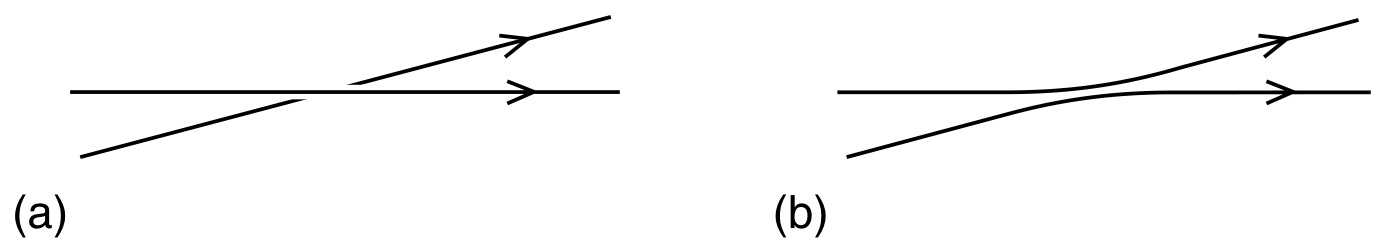
\includegraphics[width=0.8\textwidth]{figure/Fig13.4.jpg}
	\caption{(a) D-branes at relative angle. (b) Lower energy configuration.}
	\label{fig:13.4}
\end{figure}

In nonsupersymmetric configurations a tachyon can appear. For simplicity let only $\phi_1$ be nonzero, with $0 \le \phi_1 \le \pi$. The NS ground state energy is $-(1/2) + (\phi_1/2\pi)$, and the first excited state $\psi_{-1/2+(\phi_1/\pi)}^1\lvert 0\rangle_{\mathrm{NS}}$, which survives the GSO projection, has weight $-\phi_1/2\pi$. Including the energy from tension, the lightest state has
\begin{equation}
	m^2 = \frac{y_1^2}{4\pi^2{\alpha'}^2} - \frac{\phi_1}{2\pi\alpha'} \:, \quad 0 \le \phi_1 \le \pi \:. \label{13.4.27}
\end{equation}
This is negative if the separation is small enough. A special case is $\phi_1 = \pi$, when the 4-branes are antiparallel rather than parallel (a D4-brane and an anti-D4-brane). The NS--NS and R--R exchanges are then both attractive, and below the critical separation $y_1^2 = 2\pi^2\alpha'$ the cylinder amplitude diverges as $t \to \infty$. This is where the tachyon appears --- evidently it represents D4-brane/anti-D4-brane annihilation. Even when the D-branes are nearly parallel they can lower their energy by reconnecting as in Figure~\ref{fig:13.4}(b), and this is the physical origin of the instability. The decay has no end: the reconnected strings move apart indefinitely.
\begin{tcolorbox}[breakable]
	\begin{remark}
		\textbf{Conventions.} $\nu=\phi_1/\pi\in[0,1]$, the other three planes are unrotated, and the light-cone counting of the box after \eqref{13.4.8} is used. The mass-shell condition for a stretched open string is $m^2=(y_1/2\pi\alpha')^2+L_0^{\rm osc}/\alpha'$.

		\textit{NS ground-state energy.} In the rotated plane the complex boson has zero-point energy \eqref{13.4.17}. The NS fermion modes are shifted by the same $\nu$ from $\mathbb Z+\frac12$, so for a complex fermion with modes in $\mathbb Z+a$, the analogue of \eqref{13.4.17} with the opposite sign is $-\bigl[\frac1{24}-\frac12(a-\frac12)^2\bigr]$. This is $-\frac1{24}$ at $a=\frac12$ and $+\frac1{12}$ at $a=0$, as it should be. With $a=\frac12+\nu$,
		\begin{align*}
			E_{\rm plane} &= \Bigl[\frac1{24}-\frac12\Bigl(\nu-\frac12\Bigr)^2\Bigr]+\Bigl[-\frac1{24}+\frac12\nu^2\Bigr] \eqs{1} -\frac18+\frac\nu2 ,\\
			E_{\rm NS} &= 3\Bigl(-\frac18\Bigr)+\Bigl(-\frac18+\frac\nu2\Bigr) = -\frac12+\frac{\phi_1}{2\pi} .
		\end{align*}
		At (1), $\frac1{24}-\frac12\nu^2+\frac12\nu-\frac18-\frac1{24}+\frac12\nu^2=-\frac18+\frac\nu2$. The unrotated planes give $-\frac18$ each, from two NN or DD bosons and two NS fermions: $2(-\frac1{24}-\frac1{48})=-\frac18$.

		\textit{The lightest state.} The fermion mode $\psi^1_{-1/2+\nu}$ raises the energy by $\frac12-\nu$:
		\begin{equation*}
			L_0^{\rm osc} = -\frac12+\frac\nu2+\frac12-\nu = -\frac\nu2 = -\frac{\phi_1}{2\pi},\qquad
			m^2 = \frac{y_1^2}{4\pi^2{\alpha'}^2}-\frac{\phi_1}{2\pi\alpha'} ,
		\end{equation*}
		which is \eqref{13.4.27}. The NS ground state itself has the opposite GSO parity and is projected out, as for untwisted strings. At $\phi_1=\pi$ (brane and antibrane), $m^2<0$ for $y_1^2<4\pi^2\alpha'^2\cdot\frac{1}{2\alpha'}=2\pi^2\alpha'$, the critical separation quoted in the text. There the $t\to\infty$ region of the cylinder behaves as $e^{-2\pi t\alpha'm^2}$ and diverges.
	\end{remark}
\end{tcolorbox}


\section{D-Brane Interactions: Dynamics}

\subsection*{D-Brane Scattering}

For parallel static D-branes the potential energy is zero, but if they are in relative motion all supersymmetry is broken and there is a velocity-dependent force. This can be obtained by an analytic continuation of the static potential for rotated branes. Consider the case that only $\phi_1$ is nonzero, so the rotated brane satisfies $X^3 = X^2\tan\phi_1$. Analytically continue $X^2 \to \mi X'^0$ and let $\phi_1 = -\mi u$, with $u > 0$. Then
\begin{equation}
	X^3 = X'^0\tanh u \:, \label{13.5.1}
\end{equation}
which describes a D-brane moving with constant velocity. Continue also $X^0 \to -\mi X'^2$ to eliminate the spurious extra time coordinate. The interaction amplitude between the D-branes becomes
\begin{equation}
	\mathcal{A} = -\mi V_p\int_0^\infty \frac{\dif t}{t}\,(8\pi^2\alpha' t)^{-p/2}\exp\Bigl(-\frac{t y^2}{2\pi\alpha'}\Bigr)\frac{\vartheta_{11}(ut/2\pi, \mi t)^4}{\eta(\mi t)^9\,\vartheta_{11}(ut/\pi, \mi t)} \:, \label{13.5.2}
\end{equation}
where we have extended the result to general $p$ by using T-duality. It is also useful to give the modular transformation:
\begin{equation}
	\mathcal{A} = \frac{V_p}{(8\pi^2\alpha')^{p/2}}\int_0^\infty \frac{\dif t}{t}\,t^{(6-p)/2}\exp\Bigl(-\frac{t y^2}{2\pi\alpha'}\Bigr)\frac{\vartheta_{11}(\mi u/2\pi, \mi/t)^4}{\eta(\mi/t)^9\,\vartheta_{11}(\mi u/\pi, \mi/t)} \:. \label{13.5.3}
\end{equation}
\begin{tcolorbox}[breakable]
	\begin{remark}
		\textbf{Conventions.} The overall normalization of \eqref{13.5.2} is taken from the text. We derive its structure from \eqref{13.4.23} and then derive \eqref{13.5.3} from it. $\vartheta_{11}$ obeys \eqref{13.4.18a}--\eqref{13.4.18b} and is odd in $\nu$, and $\eta(\mi t)=t^{-1/2}\eta(\mi/t)$.

		\textit{\eqref{13.5.1}.} With $X^2=\mi X'^0$ and $\phi_1=-\mi u$, $\tan(-\mi u)=-\mi\tanh u$, so $X^3=X^2\tan\phi_1=\mi X'^0(-\mi\tanh u)=X'^0\tanh u$. This is a brane moving along $X^3$ with velocity $v=\tanh u<1$; $u$ is the rapidity.

		\textit{Structure of \eqref{13.5.2}.} With only $\phi_1\neq0$, \eqref{13.4.22} gives $\phi'_1=\phi'_2=\phi'_3=\phi'_4=\phi_1/2$, so the numerator of \eqref{13.4.23} is $\vartheta_{11}(\mi\phi_1t/2\pi,\mi t)^4$. The rotated plane gives the denominator $\vartheta_{11}(\mi\phi_1t/\pi,\mi t)$. Each of the three unrotated planes gives $\eta^{-3}$ by \eqref{13.4.24}--\eqref{13.4.25}, and their zero modes give the momentum and volume factors. Under $\phi_1=-\mi u$ the arguments become $\mi\phi_1t/\pi=ut/\pi$ and $ut/2\pi$, which are real, giving \eqref{13.5.2}.

		\textit{Modular transformation.} Solving \eqref{13.4.18b} for $\vartheta_{11}(\nu,\mi t)$ gives $\vartheta_{11}(\nu,\mi t)=\mi t^{-1/2}e^{-\pi\nu^2/t}\vartheta_{11}(-\mi\nu/t,\mi/t)$. Then
		\begin{align*}
			\vartheta_{11}\Bigl(\frac{ut}{2\pi},\mi t\Bigr)^4 &\eqs{1} t^{-2}e^{-u^2t/\pi}\,\vartheta_{11}\Bigl(\frac{\mi u}{2\pi},\frac{\mi}{t}\Bigr)^4, \\
			\vartheta_{11}\Bigl(\frac{ut}{\pi},\mi t\Bigr) &\eqs{2} -\mi t^{-1/2}e^{-u^2t/\pi}\,\vartheta_{11}\Bigl(\frac{\mi u}{\pi},\frac{\mi}{t}\Bigr),\\
			\frac{\vartheta_{11}(ut/2\pi,\mi t)^4}{\eta(\mi t)^9\vartheta_{11}(ut/\pi,\mi t)} \\ &\eqs{3} \frac{t^{-2}}{t^{-9/2}\cdot(-\mi)t^{-1/2}}\,\frac{\vartheta_{11}(\mi u/2\pi,\mi/t)^4}{\eta(\mi/t)^9\vartheta_{11}(\mi u/\pi,\mi/t)}\\
			&= \mi\,t^3\,\frac{\vartheta_{11}(\mi u/2\pi,\mi/t)^4}{\eta(\mi/t)^9\vartheta_{11}(\mi u/\pi,\mi/t)} .
		\end{align*}
		At (1), $(\mi t^{-1/2})^4=t^{-2}$, $4\pi(ut/2\pi)^2/t=u^2t/\pi$, and the sign of $-\mi u/2\pi$ drops out of the fourth power. At (2), $\pi(ut/\pi)^2/t=u^2t/\pi$, and oddness gives $\vartheta_{11}(-\mi u/\pi)=-\vartheta_{11}(\mi u/\pi)$. At (3), the exponentials cancel. Inserting into \eqref{13.5.2},
		\begin{align*}
			\mathcal A &= -\mi V_p\int_0^\infty\frac{\dif t}{t}(8\pi^2\alpha')^{-p/2}t^{-p/2}\cdot\mi t^3\,e^{-ty^2/2\pi\alpha'}\cdots\\ &= \frac{V_p}{(8\pi^2\alpha')^{p/2}}\int_0^\infty\frac{\dif t}{t}\,t^{(6-p)/2}e^{-ty^2/2\pi\alpha'}\cdots ,
		\end{align*}
		which is \eqref{13.5.3}.
	\end{remark}
\end{tcolorbox}

We can write this as an integral over the worldline:
\begin{equation}
	\mathcal{A} = -\mi\int_{-\infty}^{\infty}\dif\tau\:V(r(\tau), v) \:, \label{13.5.4}
\end{equation}
where
\begin{equation}
	r(\tau)^2 = y^2 + v^2\tau^2 \:, \quad v = \tanh u \:, \label{13.5.5}
\end{equation}
and
\begin{equation}
	V(r,v) = \frac{\mi}{2V_p(8\pi^2\alpha')^{(p+1)/2}}\int_0^\infty \dif t\:t^{(5-p)/2}\exp\Bigl(-\frac{t r^2}{2\pi\alpha'}\Bigr)\frac{(\tanh u)\,\vartheta_{11}(\mi u/2\pi, \mi/t)^4}{\eta(\mi/t)^9\,\vartheta_{11}(\mi u/\pi, \mi/t)} \:. \label{13.5.6}
\end{equation}

The interaction has a number of interesting properties. The first is that as $v \to 0$ (so that $u \to 0$), it vanishes as $v^4$ from the zeros of the theta functions. We expect only even powers of $v$ by time-reversal invariance. The vanishing of the $v^2$ interaction, like the vanishing of the static interaction, is a consequence of supersymmetry. The low energy field theory of the D-branes is a $\mathrm{U}(1)\times\mathrm{U}(1)$ supersymmetric gauge theory with 16 supersymmetries. What we are calculating is a correction to the effective action from integrating out massive states, strings stretched between the D-branes. The vanishing of the $v^2$ term is then consistent with the assertion that with 16 supersymmetries corrections to the kinetic term are forbidden --- the moduli space is flat. If we had instead taken $\phi_3 = \phi_4 = \pi/2$ so that $\#\mathrm{ND} = 4$, there would only be two zeros in the numerator and thus a $v^2$ interaction, consistent with the fact that kinetic corrections are allowed with 8 supercharges.

The interaction \eqref{13.5.6} is in general a complicated function of separation, but in an expansion in powers of the velocity the leading $\mathcal{O}(v^4)$ term is simple:
\begin{align}
	V(r,v) &= -\frac{v^4}{V_p(8\pi^2\alpha')^{(p+1)/2}}\int_0^\infty \dif t\:t^{(5-p)/2}\exp\Bigl(-\frac{t r^2}{2\pi\alpha'}\Bigr) + \mathcal{O}(v^6) \nonumber \\
	&= -\frac{v^4}{r^{7-p}}\frac{1}{V_p\alpha'^{p-3}}2^{2-2p}\pi^{(5-3p)/2}\Gamma\Bigl(\frac{7-p}{2}\Bigr) + \mathcal{O}(v^6) \:. \label{13.5.7}
\end{align}
At long distances this is in agreement with low energy supergravity. It is also the leading behavior if we expand in powers of $1/r$ rather than $v$.
\begin{tcolorbox}[breakable]
	\begin{remark}
		\textbf{Conventions.} Write the closed-channel ratio in \eqref{13.5.3} as $F(u,t)\equiv\vartheta_{11}(\mi u/2\pi,\mi/t)^4/[\eta(\mi/t)^9\vartheta_{11}(\mi u/\pi,\mi/t)]$. $V(r,v)$ is the full potential between the branes, so it is proportional to the brane volume $V_p$.

		\textit{From \eqref{13.5.3} to \eqref{13.5.4}--\eqref{13.5.6}.} The Gaussian integral over the trajectory $r^2=y^2+v^2\tau^2$ gives
		\begin{equation*}
			\int_{-\infty}^\infty\dif\tau\,e^{-tr(\tau)^2/2\pi\alpha'} = e^{-ty^2/2\pi\alpha'}\,\frac1v\Bigl(\frac{2\pi^2\alpha'}{t}\Bigr)^{1/2} .
		\end{equation*}
		So if $V(r,v)=C\int\dif t\,t^{a}e^{-tr^2/2\pi\alpha'}F$, then $-\mi\int\dif\tau\,V=-\mi C\,v^{-1}(2\pi^2\alpha')^{1/2}\int\dif t\,t^{a-1/2}e^{-ty^2/2\pi\alpha'}F$. Matching to \eqref{13.5.3},
		\begin{align*}
			a-\tfrac12 &= \tfrac{6-p}{2}-1 \;\Longrightarrow\; a=\tfrac{5-p}{2},\qquad
			C \eqs{1} \mi v\,V_p\,(8\pi^2\alpha')^{-p/2}(2\pi^2\alpha')^{-1/2} \eqs{2} \frac{2\mi\,V_p\tanh u}{(8\pi^2\alpha')^{(p+1)/2}} .
		\end{align*}
		At (1), $-\mi C/v=\ldots$ was solved using $1/(-\mi)=\mi$. At (2), $(2\pi^2\alpha')^{-1/2}=2(8\pi^2\alpha')^{-1/2}$ and $v=\tanh u$. The power $t^{(5-p)/2}$ agrees with \eqref{13.5.6}, but the prefactor should be $2\mi V_p\tanh u/(8\pi^2\alpha')^{(p+1)/2}$: the $V_p$ belongs in the numerator and the factor is $2\mi$, not $\mi/2$.

		\textit{Small-velocity expansion \eqref{13.5.7}.} For small argument, \eqref{13.4.18a} gives $\vartheta_{11}(\nu,\tau)=-2\pi\nu\,\eta(\tau)^3+\mathcal O(\nu^3)$, since $q^{1/8}\prod(1-q^m)^3=\eta^3$. Hence, uniformly in $t$,
		\begin{align*}
			F(u,t) &= \frac{(-2\pi\cdot\mi u/2\pi)^4\eta^{12}}{\eta^9\,(-2\pi\cdot\mi u/\pi)\,\eta^3}\bigl(1+\mathcal O(u^2)\bigr)\\ &= \frac{u^4}{-2\mi u} = \frac{\mi}{2}u^3+\mathcal O(u^5),\\
			V(r,v) &\eqs{3} \frac{2\mi V_p\tanh u}{(8\pi^2\alpha')^{(p+1)/2}}\cdot\frac{\mi}{2}u^3\int_0^\infty\dif t\,t^{(5-p)/2}e^{-tr^2/2\pi\alpha'}\\ &= -\frac{v^4V_p}{(8\pi^2\alpha')^{(p+1)/2}}\int_0^\infty\dif t\,t^{(5-p)/2}e^{-tr^2/2\pi\alpha'}+\mathcal O(v^6).
		\end{align*}
		At (3), $u^3\tanh u=v^4+\mathcal O(v^6)$. This is the first line of \eqref{13.5.7} with $V_p$ in the numerator; the coefficient 1 confirms the corrected prefactor $2\mi$. The four zeros of the numerator give $u^4$, and the single zero of the denominator removes one power, which with the $\tanh u$ gives $v^4$. With $\phi_3=\phi_4=\pi/2$ ($\#\mathrm{ND}=4$) two of the four $\phi'_a$ no longer vanish at $u=0$, so only two numerator zeros remain and the result starts at $v^2$. Doing the $t$ integral,
		\begin{align*}
			\int_0^\infty\dif t\,t^{(5-p)/2}e^{-tr^2/2\pi\alpha'} &= \Gamma\Bigl(\frac{7-p}{2}\Bigr)\Bigl(\frac{2\pi\alpha'}{r^2}\Bigr)^{(7-p)/2},\\
			\frac{(2\pi\alpha')^{(7-p)/2}}{(8\pi^2\alpha')^{(p+1)/2}} &\eqs{4} 2^{2-2p}\pi^{(5-3p)/2}{\alpha'}^{3-p},\\
			V(r,v) &= -\frac{v^4}{r^{7-p}}\,V_p\,{\alpha'}^{3-p}\,2^{2-2p}\pi^{(5-3p)/2}\,\Gamma\Bigl(\frac{7-p}{2}\Bigr)+\mathcal O(v^6).
		\end{align*}
		At (4), the powers of 2 are $\frac{7-p}{2}-\frac{3(p+1)}{2}=2-2p$ and of $\pi$ are $\frac{7-p}{2}-(p+1)=\frac{5-3p}{2}$. The numbers agree with the second line of \eqref{13.5.7}, but the volume factor there should be $V_p/\alpha'^{p-3}$ rather than $1/(V_p\alpha'^{p-3})$. The $r^{p-7}=r^{2-(9-p)}$ fall-off is the Green function in the $9-p$ transverse dimensions, as for supergravity exchange.
	\end{remark}
\end{tcolorbox}

In general the behavior of $V(r,v)$ as $r \to 0$ is quite different from the behavior as $r \to \infty$. The $r$-dependence of the integral \eqref{13.5.6} arises from the factor $\exp(-t r^2/2\pi\alpha')$, so that $t \approx 2\pi\alpha'/r^2$ governs the behavior at given $r$. Large $r$ corresponds to small $t$, where the asymptotic behavior is given by tree-level exchange of light closed strings --- hence the agreement with classical supergravity. Small $r$ corresponds to large $t$, where the asymptotic behavior is given by a loop of light open strings. The crossover is at $r^2 \sim 2\pi\alpha'$. This is as we expect: string theory modifies gravity at distances below the string scale.

To obtain the small-$r$ behavior of the scattering amplitude \eqref{13.5.6}, take the large-$t$ limit without expanding in $v$ to obtain:
\begin{equation}
	V(r,v) \approx -2V_p\int_0^\infty \frac{\dif t}{(8\pi^2\alpha' t)^{(p+1)/2}}\exp\Bigl(-\frac{t r^2}{2\pi\alpha'}\Bigr)\tanh u\,\frac{\sin^4(ut/2)}{\sin(ut)} \:. \label{13.5.8}
\end{equation}
\begin{tcolorbox}[breakable]
	\begin{remark}
		The large-$t$ limit is simplest in the open-string form \eqref{13.5.2}, where $q=e^{-2\pi t}\to0$. By \eqref{13.4.18a} with real $\nu$, $\vartheta_{11}(\nu,\mi t)\to-2q^{1/8}\sin\pi\nu$, and $\eta(\mi t)\to q^{1/24}$, so
		\begin{align*}
			\frac{\vartheta_{11}(ut/2\pi,\mi t)^4}{\eta^9\,\vartheta_{11}(ut/\pi,\mi t)} &\;\to\; \frac{16\,q^{1/2}\sin^4(ut/2)}{q^{9/24}\,(-2q^{1/8})\sin(ut)} \eqs{1} -8\,\frac{\sin^4(ut/2)}{\sin(ut)} ,\\
			\mathcal A &\approx 8\mi V_p\int_0^\infty\frac{\dif t}{t}(8\pi^2\alpha't)^{-p/2}e^{-ty^2/2\pi\alpha'}\frac{\sin^4(ut/2)}{\sin(ut)} .
		\end{align*}
		At (1), the powers of $q$ cancel, $\frac12-\frac38-\frac18=0$: only the massless open strings survive at large $t$, and these are the light stretched strings. Converting to a potential with $e^{-ty^2/2\pi\alpha'}=v\,(t/2\pi^2\alpha')^{1/2}\int\dif\tau\,e^{-tr^2/2\pi\alpha'}$ (the inverse of the Gaussian integral in the previous box) and $\mathcal A=-\mi\int\dif\tau\,V$,
		\begin{align*}
			V(r,v) &\approx -8V_p\,v\int_0^\infty\frac{\dif t}{t}(8\pi^2\alpha't)^{-p/2}\,\frac{2t^{1/2}}{(8\pi^2\alpha')^{1/2}}\,e^{-tr^2/2\pi\alpha'}\frac{\sin^4(ut/2)}{\sin(ut)}\\
			&\eqs{2} -16V_p\int_0^\infty\frac{\dif t}{(8\pi^2\alpha't)^{(p+1)/2}}\,e^{-tr^2/2\pi\alpha'}\tanh u\,\frac{\sin^4(ut/2)}{\sin(ut)} .
		\end{align*}
		At (2), $t^{-1}t^{-p/2}t^{1/2}=t^{-(p+1)/2}$ and $v=\tanh u$. The coefficient is 16, not the printed 2. As a check, expanding for small $u$, $\sin^4(ut/2)/\sin(ut)\approx u^3t^3/16$, so this gives $-v^4V_p(8\pi^2\alpha')^{-(p+1)/2}\int\dif t\,t^{(5-p)/2}e^{-tr^2/2\pi\alpha'}$, exactly the corrected \eqref{13.5.7}. With the printed 2 it would be $\frac18$ of that. The large-$t$ region is not required to have small $u t$, so \eqref{13.5.8} keeps the full dependence on $ut$.

		\textit{\eqref{13.5.9}--\eqref{13.5.12}.} The Gaussian localizes $t\approx2\pi\alpha'/r^2$, so the argument of the sines is $ut\approx2\pi\alpha'v/r^2$. The $v^4$ expansion fails and the oscillations set in when this is of order one, at $r^2\approx\alpha'v$, which is \eqref{13.5.9}. The encounter lasts $\delta t\approx r/v$, so $\delta x\,\delta t\approx r^2/v\approx\alpha'$, which is \eqref{13.5.10}. A D0-brane of mass $m=\tau_0=1/(g\alpha'^{1/2})$ from \eqref{13.3.23} with velocity spread $\delta v$ has $\delta p=m\,\delta v$, so $\delta x\gtrsim1/(m\,\delta v)$, which is \eqref{13.5.11}. Taking $\delta v\sim v$, the total uncertainty is
		\begin{equation*}
			f(v) = \alpha'^{1/2}\Bigl(v^{1/2}+\frac gv\Bigr),\qquad f'(v)=0 \;\Longrightarrow\; \frac12v^{-1/2}=\frac g{v^2} \;\Longrightarrow\; v=(2g)^{2/3}\sim g^{2/3},
		\end{equation*}
		and then $f\sim\alpha'^{1/2}(g^{1/3}+g^{1/3})\sim g^{1/3}\alpha'^{1/2}$, which is \eqref{13.5.12}.
	\end{remark}
\end{tcolorbox}
Since $t \approx 2\pi\alpha'/r^2$ and $v \approx u$, the arguments of the sines are $u t \approx 2\pi\alpha' v/r^2$. No matter how small $v$ is, the $v^4$ term will cease to dominate at small enough $r$. The oscillations of the integrand then smooth the small-$r$ behavior on a scale $u t \approx 1$. The effective scale probed by the scattering is
\begin{equation}
	r \approx \alpha'^{1/2}v^{1/2} \:. \label{13.5.9}
\end{equation}
A small-velocity D-brane probe is thus sensitive to distances shorter than the string scale! This is in contrast to the behavior seen in string scattering at weak coupling, but fits nicely with the understanding of strongly coupled strings.

A slower D-brane probes shorter distances, but the scattering process takes longer, $\delta t \approx r/v$. Then
\begin{equation}
	\delta x\,\delta t \gtrsim \alpha' \:. \label{13.5.10}
\end{equation}
This is a suggestion for a new uncertainty relation involving only the coordinates, an indication of `noncommutative geometry' connected with the promotion of D-brane collective coordinates to matrices.

For a pointlike D0-brane probe there is a minimum distance that can be measured by scattering. The wavepacket in which it is prepared satisfies:
\begin{equation}
	\delta x \gtrsim \frac{1}{m\delta v} = \frac{g\alpha'^{1/2}}{\delta v} \:. \label{13.5.11}
\end{equation}
The combined uncertainties \eqref{13.5.9} and \eqref{13.5.11} are minimized by $v \approx g^{2/3}$, for which
\begin{equation}
	\delta x \gtrsim g^{1/3}\alpha'^{1/2} \:. \label{13.5.12}
\end{equation}

\subsection*{D0-Brane Quantum Mechanics}

The nonrelativistic effective Lagrangian for $n$ D0-branes is
\begin{equation}
	L = \operatorname{Tr}\biggl(\frac{1}{2g\alpha'^{1/2}}D_0 X^i D_0 X^i + \frac{1}{4g\alpha'^{1/2}(2\pi\alpha')^2}[X^i,X^j]^2 - \frac{\mi}{2}\lambda D_0\lambda + \frac{1}{4\pi\alpha'}\lambda\Gamma^0\Gamma^i[X^i,\lambda]\biggr) \:. \label{13.5.13}
\end{equation}
The first term is the usual nonrelativistic kinetic energy with $m = \tau_0 = 1/(g\alpha'^{1/2})$, dropping the constant rest mass $n\tau_0$. The coefficients of the other terms are most easily obtained by T-duality from the ten-dimensional super-Yang--Mills action (B.6.13), with $A_i \to X^i/(2\pi\alpha')$. We have taken a basis in which the fermionic field $\lambda$ is Hermitian, and rescaled $\lambda$ to obtain a canonical kinetic term. The index $i$ runs over the nine spatial dimensions. The gauge field $A_0$ has no kinetic term but remains in the covariant derivatives. It couples to the $\mathrm{U}(n)$ charges, so its equation of motion amounts to the constraint that only $\mathrm{U}(n)$-invariant states are allowed. Only terms with at most two powers of the velocity have been kept, not the full Born--Infeld action.

The Hamiltonian is
\begin{equation}
	H = \operatorname{Tr}\biggl(\frac{g\alpha'^{1/2}}{2}p_i p_i - \frac{1}{16\pi^2 g\alpha'^{5/2}}[X^i,X^j]^2 - \frac{1}{4\pi\alpha'}\lambda\Gamma^0\Gamma^i[X^i,\lambda]\biggr) \:. \label{13.5.14}
\end{equation}
Note that the potential is positive because $[X^i,X^j]$ is anti-Hermitian. The canonical momentum, like the coordinate, is a matrix:
\begin{equation}
	[p_i^{ab}, X_j^{cd}] = -\mi\delta_{ij}\delta^{ad}\delta^{bc} \:. \label{13.5.15}
\end{equation}

Now we define
\begin{equation}
	X^i = g^{1/3}\alpha'^{1/2}Y^i \:, \label{13.5.16}
\end{equation}
so that also $p_i = p_{Y^i}/(g^{1/3}\alpha'^{1/2})$. The Hamiltonian becomes
\begin{equation}
	H = \frac{g^{1/3}}{\alpha'^{1/2}}\operatorname{Tr}\biggl(\frac{1}{2}p_{Y^i}p_{Y^i} - \frac{1}{16\pi^2}[Y^i,Y^j]^2 - \frac{1}{4\pi}\lambda\Gamma^0\Gamma^i[Y^i,\lambda]\biggr) \:. \label{13.5.17}
\end{equation}
The parameters $g$ and $\alpha'$ now appear only in the overall normalization. It follows that the wavefunctions are independent of the parameters when expressed in terms of the variables $Y^i$. In terms of the original coordinates $X^i$ their characteristic size scales as $g^{1/3}\alpha'^{1/2}$, the same scale \eqref{13.5.12} found above. The energies scale as $g^{1/3}/\alpha'^{1/2}$ from the overall normalization of $H$, and the characteristic times scale as the inverse of this, recovering the relation \eqref{13.5.10}.
\begin{tcolorbox}[breakable]
	\begin{remark}
		\textbf{Conventions.} We start from the bosonic part of ten-dimensional SYM, $-\frac{1}{4g_{\rm D0}^2}\int\operatorname{Tr}F_{MN}F^{MN}$ with $F_{MN}=\partial_MA_N-\partial_NA_M+\mi[A_M,A_N]$, reduced to $0+1$ dimensions with $A_i\to X^i/2\pi\alpha'$. The D0-brane coupling is \eqref{13.3.25} at $p=0$, $g_{\rm D0}^2=(2\pi)^{-2}g\alpha'^{-3/2}$, so $\frac1{g_{\rm D0}^2}=\frac{(2\pi)^2\alpha'^{3/2}}{g}$. The fermion normalization is taken from the text.

		\textit{Bosonic terms of \eqref{13.5.13}.}
		\begin{align*}
			F_{0i}=\frac{D_0X^i}{2\pi\alpha'},\ \ F_{ij}=\frac{\mi[X^i,X^j]}{(2\pi\alpha')^2}
			\;&\Longrightarrow\;
			-\frac1{4g_{\rm D0}^2}\operatorname{Tr}\bigl(2F_{0i}F^{0i}+F_{ij}F^{ij}\bigr)\\
			&\eqs{1} \frac{1}{2g_{\rm D0}^2}\frac{\operatorname{Tr}(D_0X^i)^2}{(2\pi\alpha')^2}+\frac{1}{4g_{\rm D0}^2}\frac{\operatorname{Tr}[X^i,X^j]^2}{(2\pi\alpha')^4},\\
			\frac{1}{2g_{\rm D0}^2(2\pi\alpha')^2} &= \frac{(2\pi)^2\alpha'^{3/2}}{2g(2\pi)^2\alpha'^2}=\frac{1}{2g\alpha'^{1/2}},\\
			\frac{1}{4g_{\rm D0}^2(2\pi\alpha')^4}&=\frac{1}{4g\alpha'^{1/2}(2\pi\alpha')^2} .
		\end{align*}
		At (1), $F^{0i}=-F_{0i}$ and $(\mi[X^i,X^j])^2=-[X^i,X^j]^2$. Both coefficients are those of \eqref{13.5.13}, and the first is $\frac12m$ with $m=\tau_0=1/(g\alpha'^{1/2})$ from \eqref{13.3.23}.

		\textit{Hamiltonian \eqref{13.5.14}.} With $p_i=\partial L/\partial(D_0X^i)=D_0X^i/(g\alpha'^{1/2})$ (as matrices, $p^{ab}_i$ conjugate to $X^{ba}_i$, which gives \eqref{13.5.15}), the Legendre transform flips the sign of every term without time derivatives:
		\begin{equation*}
			H=\operatorname{Tr}\Bigl(\frac{g\alpha'^{1/2}}{2}p_ip_i-\frac{1}{4g\alpha'^{1/2}(2\pi\alpha')^2}[X^i,X^j]^2-\frac1{4\pi\alpha'}\lambda\Gamma^0\Gamma^i[X^i,\lambda]\Bigr),
		\end{equation*}
		and $4(2\pi\alpha')^2\alpha'^{1/2}=16\pi^2\alpha'^{5/2}$, which is \eqref{13.5.14}. The first-order fermion kinetic term does not contribute to $H$. Since $[X^i,X^j]^\dagger=-[X^i,X^j]$, $\operatorname{Tr}[X^i,X^j]^2=-\operatorname{Tr}\bigl([X^i,X^j]^\dagger[X^i,X^j]\bigr)\le0$, so the potential $-\operatorname{Tr}[X,X]^2/16\pi^2g\alpha'^{5/2}$ is non-negative. It vanishes exactly on commuting matrices, which are the flat directions.

		\textit{Scaling \eqref{13.5.17}.} With $X=\ell Y$, $p=p_Y/\ell$ and $\ell=g^{1/3}\alpha'^{1/2}$, which preserves \eqref{13.5.15},
		\begin{align*}
			\frac{g\alpha'^{1/2}}{2}\frac{p_Y^2}{\ell^2} &= \frac{g^{1/3}}{\alpha'^{1/2}}\,\frac{p_Y^2}{2},\\
			\frac{\ell^4}{16\pi^2g\alpha'^{5/2}}[Y,Y]^2 &= \frac{g^{1/3}}{\alpha'^{1/2}}\,\frac{[Y,Y]^2}{16\pi^2},\\
			\frac{\ell}{4\pi\alpha'}\lambda\Gamma^0\Gamma^i[Y^i,\lambda] &= \frac{g^{1/3}}{\alpha'^{1/2}}\,\frac{\lambda\Gamma^0\Gamma^i[Y^i,\lambda]}{4\pi} .
		\end{align*}
		The three terms acquire the same prefactor because $g\alpha'^{1/2}\ell^{-2}=\ell^4/(g\alpha'^{5/2})=\ell/\alpha'$ exactly when $\ell^3=g\alpha'^{3/2}$. That is the only way to choose $\ell$, and it gives the length $g^{1/3}\alpha'^{1/2}$ of \eqref{13.5.12}. The energy scale is $g^{1/3}/\alpha'^{1/2}$, and time scale $\times$ length scale $=\alpha'^{1/2}g^{-1/3}\cdot g^{1/3}\alpha'^{1/2}=\alpha'$, which is \eqref{13.5.10}.
	\end{remark}
\end{tcolorbox}

Recall from the discussion of D-brane scattering that at distances less than the string scale only the lightest open string states contribute. In this regime the cylinder amplitude reduces to a loop amplitude in the low energy field theory \eqref{13.5.13}.

\subsection*{The $\#\mathrm{ND} = 4$ System}

Another low energy action with many applications is that for a D$p$-brane and D$p'$-brane with relative $\#\mathrm{ND} = 4$. There are three kinds of light strings: $p$-$p$, $p$-$p'$, and $p'$-$p'$, with ends on the respective D-branes. We will consider explicitly the case $p = 5$ and $p' = 9$, where we can take advantage of the $\mathrm{SO}(5,1)\times\mathrm{SO}(4)$ spacetime symmetry; all other cases are related to this by T-duality.

The 5-5 and 9-9 strings are the same as those that arise on a single D-brane. The new feature is the 5-9 strings; let us study their massless spectrum. The NS zero-point energy is zero. The moding of the fermions differs from that of the bosons by $1/2$, so there are four periodic worldsheet fermions $\psi^m$, namely those in the ND directions $m = 6, 7, 8, 9$. The four zero modes then generate $2^{4/2} = 4$ degenerate ground states, which we label by their spins in the $(6,7)$ and $(8,9)$ planes:
\begin{equation}
	\lvert s_3, s_4\rangle_{\mathrm{NS}} \:, \label{13.5.18}
\end{equation}
with $s_3, s_4 = \pm 1/2$. Now we need to impose the GSO projection. This was defined in \eqref{10.2.22} in terms of $s_a$, so that with the extra sign from the ghosts it is
\begin{equation}
	-\exp\bigl(\pi\mi(s_3 + s_4)\bigr) = +1 \quad \Longrightarrow \quad s_3 = s_4 \:. \label{13.5.19}
\end{equation}
In terms of symmetries, the four states \eqref{13.5.18} are invariant under $\mathrm{SO}(5,1)$ and form spinors $\mathbf{2} + \mathbf{2}'$ of the `internal' $\mathrm{SO}(4)$, and only the $\mathbf{2}$ survives the GSO projection. In the R sector, of the transverse fermions $\psi^i$ only those with $i = 2, 3, 4, 5$ are periodic, so there are again four ground states:
\begin{equation}
	\lvert s_1, s_2\rangle_{\mathrm{R}} \:. \label{13.5.20}
\end{equation}
The GSO projection does not have an extra sign in the R sector so it requires $s_1 = -s_2$. The surviving spinors are invariant under the internal $\mathrm{SO}(4)$ and form a $\mathbf{2}'$ of the $\mathrm{SO}(4)$ little group of a massless particle.
\begin{tcolorbox}[breakable]
	\begin{remark}
		\textbf{Conventions.} Light-cone directions are $0,1$; the NN directions transverse to the light cone are $2,3,4,5$, and the ND directions are $6,7,8,9$. As in \eqref{10.2.22}, $\exp(\pi\mi F)$ acts on a zero-mode ground state as $\exp\bigl(\pi\mi\sum s_a\bigr)$ over the planes with zero modes, with an extra $-1$ in the NS sector from the ghosts. The physical states have $\exp(\pi\mi F)=+1$.

		\textit{NS sector.} By \eqref{13.4.8} with $\#\mathrm{ND}=4$, the zero-point energy is $-\frac12+\frac48=0$. The NS fermions $\psi^{6,7,8,9}$ are integer-moded and have zero modes, and $\{\psi^m_0,\psi^n_0\}=\delta^{mn}$ generates a Clifford algebra with $2^{4/2}=4$ states $|s_3,s_4\rangle$ ($s_3$ for the $(6,7)$ plane, $s_4$ for $(8,9)$). Then
		\begin{equation*}
			-e^{\pi\mi(s_3+s_4)}=+1 \;\Longleftrightarrow\; s_3+s_4\in\{\pm1\} \;\Longleftrightarrow\; s_3=s_4 .
		\end{equation*}
		These two states have $\prod2s=+1$ in the internal SO(4), which is one of its two-dimensional spinors, the $\mathbf 2$. The internal SO(4) is the rotation group of the ND directions; SO(4)$\,\cong\,$SU(2)$\times$SU(2), and its spinors are $\mathbf2=(\mathbf2,\mathbf1)$ and $\mathbf2'=(\mathbf1,\mathbf2)$. They carry no spacetime spin, so they are scalars of SO(5,1).

		\textit{R sector.} The zero-point energy is $0$, and the integer-moded fermions are now those in the NN directions, $\psi^{2,3,4,5}$, giving $|s_1,s_2\rangle$ with $s_1$ for $(2,3)$ and $s_2$ for $(4,5)$. With no ghost sign,
		\begin{equation*}
			e^{\pi\mi(s_1+s_2)}=+1 \;\Longleftrightarrow\; s_1+s_2=0 \;\Longleftrightarrow\; s_1=-s_2 ,
		\end{equation*}
		which is a two-component spinor of the SO(4) little group of a massless particle in six dimensions, of definite chirality ($\prod2s=-1$, the $\mathbf2'$). The 5-9 string is oriented, so its fields are complex, and its massless content is a doublet $\chi_i$ of complex scalars under the internal SU(2) plus one chiral spinor: half a hypermultiplet. The 9-5 strings supply the conjugate half. Which chirality survives in each sector depends on the sign conventions in \eqref{10.2.22}; the physical point is that the GSO projection keeps one of the two in each sector.
	\end{remark}
\end{tcolorbox}

The system has six-dimensional Lorentz invariance and eight unbroken supersymmetries, so we can classify it by $d = 6, N = 1$ supersymmetry (section B.7). The massless content of the 5-9 spectrum amounts to half of a hypermultiplet. The other half comes from strings of opposite orientation, 9-5. The action is fully determined by supersymmetry and the charges; we write the bosonic part:
\begin{equation}
	S = -\frac{1}{4g_{\mathrm{D}9}^2}\int \dif^{10}x\,F_{MN}F^{MN} - \frac{1}{4g_{\mathrm{D}5}^2}\int \dif^6 x\,F'_{MN}F'^{MN} - \int \dif^6 x\,\Bigl(D_\mu\chi^\dagger D^\mu\chi + \frac{g_{\mathrm{D}5}^2}{2}\sum_{A=1}^3(\chi_i^\dagger\sigma_{ij}^A\chi_j)^2\Bigr) \:. \label{13.5.21}
\end{equation}
The integrals run respectively over the 9-brane and the 5-brane, with $M = 0,\dots,9$, $\mu = 0,\dots,5$, and $m = 6,\dots,9$. The covariant derivative is $D_\mu = \del_\mu + \mi A_\mu - \mi A'_\mu$ with $A_\mu$ and $A'_\mu$ the 9-brane and 5-brane gauge fields. The field $\chi_i$ is a doublet describing the hypermultiplet scalars. The 5-9 strings have one endpoint on each D-brane so $\chi$ carries charges $+1$ and $-1$ under the respective symmetries. The gauge couplings $g_{\mathrm{D}p}$ were given in \eqref{13.3.25}. We are using a condensed notation:
\begin{equation}
	A'_M \longrightarrow A'_\mu \:, \quad X'^m/(2\pi\alpha') \:. \label{13.5.22}
\end{equation}
The massless 5-5 (and also 9-9) strings separate into $d = 6, N = 1$ vector and hypermultiplets. The final potential term is the 5-5 D-term required by supersymmetry. One might have expected a 9-9 D-term as well by T-duality, but this is inversely proportional to the volume of the D9-brane in the $(6,7,8,9)$-directions, which we have taken to be infinite.

Under T-dualities in any of the ND directions, one obtains $(p, p') = (8,6), (7,7), (6,8)$, or $(5,9)$, but the intersection of the branes remains $(5+1)$-dimensional and the $p$-$p'$ strings live on the intersection with action \eqref{13.5.21}. T-dualities in $r$ NN directions give $(p, p') = (9-r, 5-r)$. The vector components in the dualized directions become collective coordinates as usual:
\begin{equation}
	A_i \longrightarrow X^i/(2\pi\alpha') \:, \quad A'_i \longrightarrow X'^i/(2\pi\alpha') \:. \label{13.5.23}
\end{equation}
The term $D_i\chi^\dagger D_i\chi$ then becomes
\begin{equation}
	\biggl(\frac{X^i - X'^i}{2\pi\alpha'}\biggr)^2\chi^\dagger\chi \:. \label{13.5.24}
\end{equation}
This just reflects the fact that when the $(9-r)$-brane and $(5-r)$-brane are separated, the strings stretched between them become massive. The action for several branes of each type is given by the non-Abelian extension.
\begin{tcolorbox}[breakable]
	\begin{remark}
		In a dualized direction $i$ the fields no longer depend on $x^i$, so $\partial_i\chi=0$, and \eqref{13.5.23} turns the covariant derivative into
		\begin{align*}
			D_i\chi = \bigl(\partial_i+\mi A_i-\mi A'_i\bigr)\chi \eqs{1} \frac{\mi\,(X^i-X'^i)}{2\pi\alpha'}\chi
			\;\Longrightarrow\; D_i\chi^\dagger D_i\chi = \Bigl(\frac{X^i-X'^i}{2\pi\alpha'}\Bigr)^2\chi^\dagger\chi ,
		\end{align*}
		which is \eqref{13.5.24}. At (1), the charges $+1$ and $-1$ of $\chi$ under the two gauge groups were used. The mass term in $-\int D\chi^\dagger D\chi$ is $m^2=(\Delta X/2\pi\alpha')^2$, exactly the mass of a string of tension $1/2\pi\alpha'$ stretched over the separation $\Delta X$. This is the same stretching term as $e^{-ty^2/2\pi\alpha'}$ in the cylinder amplitudes, since $e^{-2\pi t\alpha'm^2}=e^{-t\Delta X^2/2\pi\alpha'}$. Under T-duality along NN directions, $(p,p')\to(9-r,5-r)$, and the ND count stays 4 because NN directions become DD, not ND.
	\end{remark}
\end{tcolorbox}


\section{D-Brane Interactions: Bound States}

Bound states of D-branes with strings and with each other, and supersymmetric bound states in particular, present a number of interesting dynamical problems. Further, these bound states will play an important role in the next chapter in our attempts to deduce the strongly coupled behavior of string theory.

\subsection*{$(p,q)$ String Bound States}

The first case we consider is a state with $p$ F-strings and $q$ D-strings in the IIB theory, all at rest and aligned along the 1-direction. For a state with these charges, the supersymmetry algebra \eqref{13.2.9} becomes
\begin{equation}
	\frac{1}{2}\begin{Bmatrix} Q_\alpha \\ \tilde{Q}_\alpha \end{Bmatrix}\begin{Bmatrix} Q_\beta^\dagger & \tilde{Q}_\beta^\dagger \end{Bmatrix} = M\delta_{\alpha\beta}\begin{pmatrix} 1 & 0 \\ 0 & 1 \end{pmatrix} + \frac{L_1}{2\pi\alpha'}(\Gamma^0\Gamma^1)_{\alpha\beta}\begin{pmatrix} p & q/g \\ q/g & -p \end{pmatrix} \:, \label{13.6.1}
\end{equation}
where $L_1$ is the length of the system. The eigenvalues of $\Gamma^0\Gamma^1$ are $\pm 1$, so those of the right-hand side are
\begin{equation}
	M \pm \frac{L_1(p^2 + q^2/g^2)^{1/2}}{2\pi\alpha'} \:. \label{13.6.2}
\end{equation}
The left-hand side of the algebra is positive --- its expectation value in any state is a matrix with positive eigenvalues. This implies a BPS bound on the total energy per unit length:
\begin{equation}
	\frac{M}{L_1} \ge \frac{(p^2 + q^2/g^2)^{1/2}}{2\pi\alpha'} \:. \label{13.6.3}
\end{equation}
This inequality is saturated by the F-string, which has $(p,q) = (1,0)$, and by the D-string, with $(p,q) = (0,1)$.
\begin{tcolorbox}[breakable]
	\begin{remark}
		\textbf{Conventions.} As in the BPS box after \eqref{13.2.10}: a Majorana basis, $\mathcal C=\Gamma^0$, and a static state at rest with $P^0=M$. The strings lie along $x^1$ with length $L_1$, so $Q^1_{\rm NS}=pL_1$ and the D-string charge is $qL_1$, with charges normalized to one per unit length as stated below \eqref{13.2.9}.

		\textit{The entries of \eqref{13.6.1}.} By \eqref{13.2.9a}--\eqref{13.2.9b} the diagonal blocks are $M\delta_{\alpha\beta}\pm\frac{pL_1}{2\pi\alpha'}(\Gamma^0\Gamma^1)_{\alpha\beta}$, with opposite signs for $Q$ and $\tilde Q$. By \eqref{13.2.9c} the off-diagonal block is $\tau_1Q_{\rm R}^1(\Gamma^0\beta_1)$, and $\tau_{\rm D1}=1/(2\pi\alpha'g)$ from \eqref{13.3.23}, so it is $\frac{qL_1}{2\pi\alpha' g}$ times a matrix that can be brought to $\Gamma^0\Gamma^1$ by a redefinition of $\tilde Q$ (as in \eqref{13.2.10}).

		\textit{Eigenvalues.} The two factors commute and act on different indices, so the eigenvalues of the product are products of eigenvalues:
		\begin{align*}
			(\Gamma^0\Gamma^1)^2 &= -\Gamma^0\Gamma^0\Gamma^1\Gamma^1 \eqs{1} 1 ,\\
			\det\begin{pmatrix} p-\lambda & q/g \\ q/g & -p-\lambda\end{pmatrix} &= \lambda^2-p^2-\frac{q^2}{g^2}=0 \;\Longrightarrow\; \lambda=\pm\Bigl(p^2+\frac{q^2}{g^2}\Bigr)^{1/2} .
		\end{align*}
		At (1), $(\Gamma^0)^2=-1$ and $(\Gamma^1)^2=+1$; $\Gamma^0\Gamma^1$ is traceless, so its eigenvalues $\pm1$ each occur 16 times. The right-hand side of \eqref{13.6.1} therefore has eigenvalues $M\pm L_1(p^2+q^2/g^2)^{1/2}/2\pi\alpha'$, which is \eqref{13.6.2}. The left-hand side has the form $\frac12\sum\mathcal Q\mathcal Q^\dagger$, whose expectation value is $\frac12\|\mathcal Q^\dagger|\psi\rangle\|^2\ge0$, so the smaller eigenvalue must be non-negative, which is \eqref{13.6.3}. The bound is saturated when half the 32 supercharges annihilate the state. For $(1,0)$ it gives $1/2\pi\alpha'=\tau_{\rm F1}$, and for $(0,1)$ it gives $1/2\pi\alpha'g=\tau_{\rm D1}$, the known tensions.
	\end{remark}
\end{tcolorbox}

For one F-string and one D-string, the total energy per unit length is
\begin{equation}
	\tau_{(0,1)} + \tau_{(1,0)} = \frac{g^{-1} + 1}{2\pi\alpha'} \:. \label{13.6.4}
\end{equation}
This exceeds the BPS bound
\begin{equation}
	\tau_{(1,1)} = \frac{(g^{-2} + 1)^{1/2}}{2\pi\alpha'} \:, \label{13.6.5}
\end{equation}
and so this configuration is not supersymmetric. One can also see this directly. The F-string is invariant under supersymmetries satisfying
\begin{equation}
	\text{left-moving: } \Gamma^0\Gamma^1 Q = Q \:, \quad \text{right-moving: } \Gamma^0\Gamma^1\tilde{Q} = -\tilde{Q} \:, \label{13.6.6}
\end{equation}
and no linear combination of these is of the form $Q_\alpha + (\beta_\perp\tilde{Q})_\alpha$ preserved by the D-string (note that $\beta_\perp\Gamma^0\Gamma^1 = \Gamma^0\Gamma^1\beta_\perp$).

\begin{figure}[htbp]
	\centering
	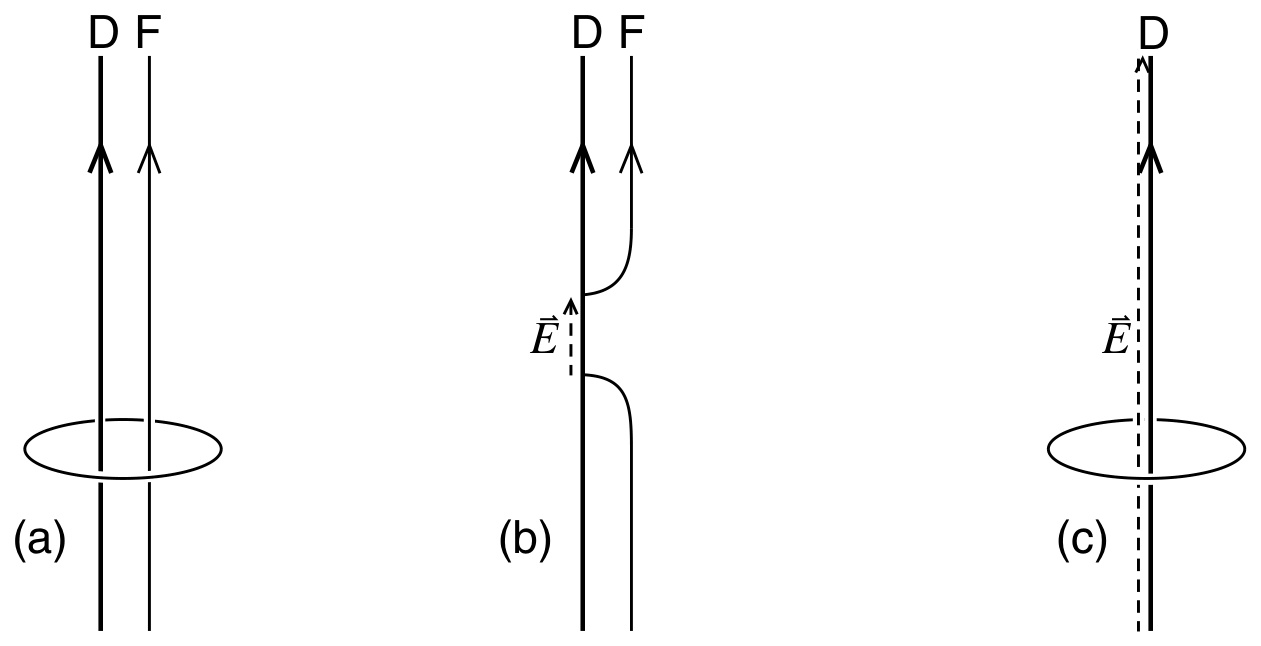
\includegraphics[width=0.75\textwidth]{figure/Fig13.5.jpg}
	\caption{(a) Parallel D-string and F-string. The loop signifies a 7-sphere surrounding the strings. (b) The F-string breaks, its ends attaching to the D-string. (c) Final state: D-string with flux.}
	\label{fig:13.5}
\end{figure}

However, the system can lower its energy as shown in Figure~\ref{fig:13.5}. The F-string breaks, with its endpoints attached to the D-string. The endpoints can then move off to infinity, leaving only the D-string behind. This cannot be the whole story because the F-string carries the NS--NS 2-form charge, as measured by the integral of $*H_{\textit{3}}$ over the 7-sphere in the figure: this flux must still be nonzero in the final configuration. This comes about because the F-string endpoints are charged under the D-string gauge field, so an electric flux runs between them. This flux remains in the end. Further, from the D-string action
\begin{equation}
	S_1 = -T_1\int \dif^2\xi\,\me^{-\Phi}\sqrt{-\det(G_{ab} + B_{ab} + 2\pi\alpha' F_{ab})} \:, \label{13.6.7}
\end{equation}
one sees that $B_{\mu\nu}$ has a source proportional to the invariant electric flux $\mathcal{F}_{ab} = F_{ab} + B_{ab}/(2\pi\alpha')$ on the D-string.

The simplest way to see that the resulting state is supersymmetric is via T-duality along the 1-direction. The D1-brane becomes a D0-brane. The electric field is T-dual to a velocity, $\dot{A}_1 \to \dot{X}^1/(2\pi\alpha')$, so the T-dual state is a D0-brane moving with constant velocity. This is invariant under the same number of supersymmetries as a D-brane at rest, namely the Lorentz boost of those supersymmetries. The boosted supersymmetries are linear combinations of the unbroken and broken supersymmetries of the D0-brane at rest. All of this carries over by T-duality to the D1--F1 system. We leave it as an exercise to verify that the tension takes the BPS value.

The F-string `dissolves' in the D-string, leaving flux behind. For separated D- and F-strings there is an attractive force at long distance, a consequence of the lack of supersymmetry. One might have expected that the binding energy would be of order $g$, the typical scale for D-brane processes, but the binding tension
\begin{equation}
	\tau_{(1,0)} + \tau_{(0,1)} - \tau_{(1,1)} = \frac{1 - \mathcal{O}(g)}{2\pi\alpha'} \label{13.6.8}
\end{equation}
is almost the total tension of the F-string.
\begin{tcolorbox}[breakable]
	\begin{remark}
		\textit{\eqref{13.6.4}--\eqref{13.6.8}.} With $\tau_{(1,0)}=1/2\pi\alpha'$ and $\tau_{(0,1)}=1/2\pi\alpha'g$,
		\begin{align*}
			2\pi\alpha'\tau_{(1,1)} = (g^{-2}+1)^{1/2} = g^{-1}(1+g^2)^{1/2} \eqs{1} g^{-1}+\frac g2-\frac{g^3}{8}+\cdots,\\
			2\pi\alpha'\bigl(\tau_{(1,0)}+\tau_{(0,1)}-\tau_{(1,1)}\bigr) = 1-\frac g2+\mathcal O(g^3) .
		\end{align*}
		At (1), $(1+x)^{1/2}=1+\frac x2-\frac{x^2}8+\cdots$. The binding energy is the whole F-string tension up to $\mathcal O(g)$: for $g\to0$ the bound F-string costs only the energy $\frac{g}{2}\cdot\frac1{2\pi\alpha'}$ of the electric flux on the heavy D-string.

		\textit{The exercise: the tension of the D-string with flux.} Take \eqref{13.6.7} with constant dilaton ($T_1e^{-\Phi}=\tau_1$), $B=0$, flat metric, and a constant electric field $F_{01}=E$ along the string. With $x=2\pi\alpha'E$, $-\det(\eta_{ab}+2\pi\alpha'F_{ab})=1-x^2$, and
		\begin{align*}
			\mathcal L &= -\tau_1(1-x^2)^{1/2},\qquad
			\Pi=\frac{\partial\mathcal L}{\partial E}=\frac{2\pi\alpha'\tau_1x}{(1-x^2)^{1/2}},\\
			\mathcal H &= \Pi E-\mathcal L \eqs{2} \frac{\tau_1}{(1-x^2)^{1/2}} \;\Longrightarrow\; \mathcal H^2 = \tau_1^2+\frac{\tau_1^2x^2}{1-x^2} = \tau_1^2+\Bigl(\frac{\Pi}{2\pi\alpha'}\Bigr)^2 .
		\end{align*}
		At (2), $\Pi E=\tau_1x^2/(1-x^2)^{1/2}$ and $x^2/(1-x^2)^{1/2}+(1-x^2)^{1/2}=(1-x^2)^{-1/2}$. The momentum $\Pi$ conjugate to $A_1$ is quantized in integers on a compact string, because large gauge transformations shift the holonomy of $A_1$ by $2\pi$. The endpoints of the F-strings are its unit charges, so $\Pi=p$ for $p$ dissolved F-strings. Then
		\begin{equation*}
			\mathcal H = \Bigl(\frac1{(2\pi\alpha'g)^2}+\frac{p^2}{(2\pi\alpha')^2}\Bigr)^{1/2} = \frac{(p^2+g^{-2})^{1/2}}{2\pi\alpha'} = \tau_{(p,1)} ,
		\end{equation*}
		exactly the BPS value \eqref{13.6.3} with $q=1$. The T-dual statement is the relativistic energy $\tau_0/(1-v^2)^{1/2}$ of the moving D0-brane, with $v=2\pi\alpha'\dot A_1=x$.
	\end{remark}
\end{tcolorbox}

String theory with a constant open string field strength has a simple worldsheet description. The variation of the worldsheet action includes a surface term:
\begin{equation}
	\int_{\del\mathcal{M}}\dif s\:\delta X^\mu\Bigl(\frac{1}{2\pi\alpha'}\del_n X_\mu + \mi F_{\mu\nu}\del_t X^\nu\Bigr) \:, \label{13.6.9}
\end{equation}
implying the linear boundary condition:
\begin{equation}
	\del_n X^\mu + 2\pi\alpha'\mi F^{\mu\nu}\del_t X_\nu = 0 \:. \label{13.6.10}
\end{equation}
\begin{tcolorbox}[breakable]
	\begin{remark}
		\textbf{Conventions.} Euclidean world-sheet action $S=\frac{1}{4\pi\alpha'}\int_{\mathcal M}\dif^2\sigma\,\partial_aX^\mu\partial_aX_\mu-\mi\int_{\partial\mathcal M}\dif s\,A_\mu\partial_tX^\mu$, where the boundary coupling is the Wilson line for a charge at the string endpoint. $\partial_n$ and $\partial_t$ are the normal and tangential derivatives, and the orientation signs are those of the text.

		\textit{The surface term.} Varying the bulk term and integrating by parts leaves the boundary piece $\frac{1}{2\pi\alpha'}\int\dif s\,\delta X^\mu\partial_nX_\mu$. For the Wilson line,
		\begin{align*}
			\delta\int\dif s\,A_\mu\partial_tX^\mu &= \int\dif s\bigl(\partial_\nu A_\mu\,\delta X^\nu\,\partial_tX^\mu+A_\mu\partial_t\delta X^\mu\bigr)\\
			&\eqs{1} \int\dif s\,\delta X^\nu\bigl(\partial_\nu A_\mu-\partial_\mu A_\nu\bigr)\partial_tX^\mu = \int\dif s\,\delta X^\nu F_{\nu\mu}\partial_tX^\mu .
		\end{align*}
		At (1), $A_\mu\partial_t\delta X^\mu$ was integrated by parts along the closed boundary, and $\partial_tA_\mu=\partial_\nu A_\mu\,\partial_tX^\nu$. So $-\mi\times$ this, relabelled, together with the bulk piece gives the total surface term \eqref{13.6.9}, $\int\dif s\,\delta X^\mu\bigl(\frac{1}{2\pi\alpha'}\partial_nX_\mu+\mi F_{\mu\nu}\partial_tX^\nu\bigr)$, up to the overall orientation sign. For $\delta X^\mu$ free on the boundary (Neumann directions of the D-brane), the bracket must vanish; multiplying by $2\pi\alpha'$ and raising the index gives \eqref{13.6.10}. Only the gauge-invariant $F$ appears. The condition interpolates linearly between Neumann ($F=0$) and, as $F\to\infty$, Dirichlet ($\partial_tX=0$), which is the world-sheet version of the T-duality between flux and tilted branes.
	\end{remark}
\end{tcolorbox}

All of the above extends immediately to $p$ F-strings and one D-string forming a supersymmetric $(p,1)$ bound state. The general case of $p$ F-strings and $q$ D-strings is more complicated because the gauge dynamics on the D-strings is non-Abelian. A two-dimensional gauge coupling has units of inverse length-squared: $g_{\mathrm{D}1}^2 = g/(2\pi\alpha')$. For dynamics on length scale $l$ the effective dimensionless coupling is $g l^2/(2\pi\alpha')$. No matter how weak the underlying string coupling $g$, the D-string dynamics at long distances is strongly coupled.

Focus for example on two D-strings and one F-string. There is a state with a separated $(1,1)$ bound state and $(0,1)$ D-string. The tension
\begin{equation}
	\tau_{(1,1)} + \tau_{(0,1)} = \frac{(g^{-2} + 1)^{1/2} + g^{-1}}{2\pi\alpha'} = \frac{2g^{-1} + g/2 + \mathcal{O}(g^3)}{2\pi\alpha'} \label{13.6.11}
\end{equation}
exceeds the BPS bound
\begin{equation}
	\tau_{(1,2)} = \frac{(4g^{-2} + 1)^{1/2}}{2\pi\alpha'} = \frac{2g^{-1} + g/4 + \mathcal{O}(g^3)}{2\pi\alpha'} \:. \label{13.6.12}
\end{equation}
The electric flux is on the first D-brane, so as a $\mathrm{U}(2)$ matrix this is proportional to:
\begin{equation}
	\begin{pmatrix} 1 & 0 \\ 0 & 0 \end{pmatrix} = \frac{1}{2}\begin{pmatrix} 1 & 0 \\ 0 & 1 \end{pmatrix} + \frac{1}{2}\begin{pmatrix} 1 & 0 \\ 0 & -1 \end{pmatrix} \:. \label{13.6.13}
\end{equation}
We have separated this into $\mathrm{U}(1)$ and $\mathrm{SU}(2)$ pieces. When we bring the two D-strings together, the $\mathrm{SU}(2)$ field becomes strongly coupled but the $\mathrm{U}(1)$ part remains free. If the $\mathrm{SU}(2)$ part is screened by the massless fields on the D-strings, then the total energy in the flux is reduced by a factor of 2, from \eqref{13.6.11} to the BPS value \eqref{13.6.12}.
\begin{tcolorbox}[breakable]
	\begin{remark}
		\textit{Expansions.} With $(1+x)^{1/2}=1+\frac x2+\cdots$,
		\begin{align*}
			(g^{-2}+1)^{1/2}+g^{-1} &= 2g^{-1}+\frac g2+\mathcal O(g^3),\\
			(4g^{-2}+1)^{1/2} &= 2g^{-1}\Bigl(1+\frac{g^2}{4}\Bigr)^{1/2} = 2g^{-1}+\frac g4+\mathcal O(g^3),
		\end{align*}
		which are \eqref{13.6.11} and \eqref{13.6.12}. The rest-energy $2g^{-1}/2\pi\alpha'$ of the two D-strings is common, and the flux energy is $\frac{g}{2}$ versus $\frac g4$ in units of $1/2\pi\alpha'$.

		\textit{Why the factor is 2.} At weak coupling the flux energy is the electric energy $\frac{g_{\rm D1}^2}{2}\operatorname{Tr}(\Pi^2)$ of the D-string gauge theory per unit length, the analogue of $\frac12E^2$. For unit flux on one of two strings, $\Pi=\mathrm{diag}(1,0)$ and $\operatorname{Tr}\Pi^2=1$. After screening of the SU(2) part only the U(1) part $\frac12\mathbb 1$ of \eqref{13.6.13} remains, with $\operatorname{Tr}(\frac12\mathbb 1)^2=\frac12$. The ratio $\frac12$ is exactly $(g/4)/(g/2)$. The same check with $g_{\rm D1}^2=g/2\pi\alpha'$ fixes the absolute value: for one string $\frac{g}{2\cdot2\pi\alpha'}$, matching $\tau_{(1,1)}-\tau_{(0,1)}$ at order $g$.
	\end{remark}
\end{tcolorbox}

Focus on four of the 16 supersymmetries, forming the equivalent of $d = 4, N = 1$ supersymmetry. The six scalars $X^{4,\dots,9}$ can be written as three chiral superfields $\Phi^i$, with the potential coming from a superpotential $\operatorname{Tr}(\Phi^1[\Phi^2,\Phi^3])$. Adding a mass term to the superpotential:
\begin{equation}
	W(\Phi) = \operatorname{Tr}(\Phi^1[\Phi^2,\Phi^3]) + m\operatorname{Tr}(\Phi^i\Phi^i) \label{13.6.14}
\end{equation}
breaks the gauge group to $\mathrm{SU}(2)$ and lifts the flat directions. Its mass cannot depend on $m$ by the BPS property. Increasing $m$ reduces the effective dimensionless coupling $g/(2\pi\alpha' m^2)$ to a value where the system becomes weakly coupled, establishing the existence of the supersymmetric $(p,q)$ bound string for all coprime $p$ and $q$.

\subsection*{D0--D$p$ BPS Bounds}

For a system with the charges of a D0-brane and a D$p$-brane extended in the $(1,\dots,p)$-directions, the supersymmetry algebra becomes
\begin{equation}
	\frac{1}{2}\begin{Bmatrix} Q_\alpha \\ \tilde{Q}_\alpha \end{Bmatrix}\begin{Bmatrix} Q_\beta^\dagger & \tilde{Q}_\beta^\dagger \end{Bmatrix} = M\begin{pmatrix} 1 & 0 \\ 0 & 1 \end{pmatrix}\delta_{\alpha\beta} + \begin{pmatrix} 0 & Z \\ -Z^\dagger & 0 \end{pmatrix}(\Gamma^0)_{\alpha\beta} \:, \label{13.6.15}
\end{equation}
where
\begin{equation}
	Z = \tau_0 + \tau_p V_p\beta \:, \quad \beta = \beta_1\cdots\beta_p \:. \label{13.6.16}
\end{equation}
We have wrapped the D$p$-brane on a torus of volume $V_p$ so that its mass will be finite. The positivity of the left-hand side implies that
\begin{subequations} \label{13.6.17}
	\begin{align}
		M^2\begin{pmatrix} 1 & 0 \\ 0 & 1 \end{pmatrix} &\ge \begin{pmatrix} 0 & Z \\ -Z^\dagger & 0 \end{pmatrix}\Gamma^0\begin{pmatrix} 0 & Z \\ -Z^\dagger & 0 \end{pmatrix}\Gamma^0 = \begin{pmatrix} ZZ^\dagger & 0 \\ 0 & Z^\dagger Z \end{pmatrix} \:, \label{13.6.17a} \\
		ZZ^\dagger &= \tau_0^2 + \tau_0\tau_p V_p(\beta + \beta^\dagger) + \tau_p^2 V_p^2\beta\beta^\dagger \:. \label{13.6.17b}
	\end{align}
\end{subequations}

For $p$ a multiple of 4, $\beta$ is Hermitian and $\beta^2 = 1$. The BPS bound is then
\begin{equation}
	M \ge \tau_0 + \tau_p V_p \:. \label{13.6.18}
\end{equation}
For $p = 4k + 2$, $\beta$ is anti-Hermitian, $\beta^2 = -1$, and the BPS bound is
\begin{equation}
	M \ge \bigl(\tau_0^2 + \tau_p^2 V_p^2\bigr)^{1/2} \:. \label{13.6.19}
\end{equation}
These bounds are consistent with our earlier results on supersymmetry breaking, noting that $\#\mathrm{ND} = p$. For $p = 4k$, a separated 0-brane and $p$-brane saturate the BPS bound \eqref{13.6.18}. For $p = 4k + 2$ they do not saturate the bound and so cannot be in a BPS state.
\begin{tcolorbox}[breakable]
	\begin{remark}
		\textbf{Conventions.} Majorana basis, so $\Gamma^0$ is real antisymmetric ($\Gamma^{0\dagger}=-\Gamma^0$) and each $\beta_m$ is real orthogonal; $\beta=\beta_1\cdots\beta_p$ with $p$ even. Write $K=\begin{pmatrix}0&Z\\-Z^\dagger&0\end{pmatrix}\Gamma^0$ for the second term of \eqref{13.6.15}.

		\textit{$K$ is Hermitian with a symmetric spectrum.} $\Gamma^0$ commutes with the spatial $\beta_m$ (box after \eqref{13.2.10}), hence with $Z$ and $Z^\dagger$. Then $(Z\Gamma^0)^\dagger=\Gamma^{0\dagger}Z^\dagger=-Z^\dagger\Gamma^0$, so the off-diagonal blocks of $K$ are adjoints of each other and $K$ is Hermitian. Also $\sigma_3K\sigma_3=-K$ with $\sigma_3=\mathrm{diag}(1,-1)$ in the $(Q,\tilde Q)$ index, so the eigenvalues of $K$ come in pairs $\pm\kappa$. Positivity of $M+K$ therefore means $M\ge|\kappa|$ for every eigenvalue, i.e.\ $M^2\ge K^2$:
		\begin{align*}
			K^2 = \begin{pmatrix}0&Z\\-Z^\dagger&0\end{pmatrix}^2(\Gamma^0)^2 \eqs{1} -\begin{pmatrix}-ZZ^\dagger&0\\0&-Z^\dagger Z\end{pmatrix} = \begin{pmatrix}ZZ^\dagger&0\\0&Z^\dagger Z\end{pmatrix},
		\end{align*}
		where (1) uses $[\Gamma^0,Z]=0$ and $(\Gamma^0)^2=-1$. This is \eqref{13.6.17a}, and expanding $ZZ^\dagger$ with $Z=\tau_0+\tau_pV_p\beta$ gives \eqref{13.6.17b}.

		\textit{Hermiticity of $\beta$.} Since $\beta$ is real orthogonal, $\beta^\dagger=\beta^{\mathrm T}=\beta^{-1}$, and by the computation \eqref{bsq} with $p$ factors,
		\begin{gather*}
			\beta^2=(-1)^{p(p+1)/2}=\begin{cases}+1 & p=4k,\\ -1 & p=4k+2,\end{cases}\\
			\beta^\dagger=\beta^{-1}=\begin{cases}+\beta & p=4k \ (\text{Hermitian}),\\ -\beta & p=4k+2 \ (\text{anti-Hermitian}).\end{cases}
		\end{gather*}
		For $p=4k$: $p(p+1)/2=2k(4k+1)$ is even. For $p=4k+2$: $(2k+1)(4k+3)$ is odd.

		\textit{The bounds.} With $\beta\beta^\dagger=1$:
		\begin{align*}
			p=4k:&\quad ZZ^\dagger=\tau_0^2+2\tau_0\tau_pV_p\,\beta+\tau_p^2V_p^2,\ \ \beta=\pm1\text{ on eigenvectors}\\ &\quad\;\Longrightarrow\; M^2\ge(\tau_0+\tau_pV_p)^2,\\
			p=4k+2:&\quad \beta+\beta^\dagger=0 \;\Longrightarrow\; ZZ^\dagger=\tau_0^2+\tau_p^2V_p^2 \;\Longrightarrow\; M^2\ge\tau_0^2+\tau_p^2V_p^2 ,
		\end{align*}
		which are \eqref{13.6.18} and \eqref{13.6.19}. Since $\#\mathrm{ND}=p$ for D0--D$p$, this matches the box after the $\#\mathrm{ND}$ list. For $p=4,8$ the separated branes have $M=\tau_0+\tau_pV_p$, saturate the bound, and preserve 8 supercharges (the $\beta=+1$ eigenspace). For $p=2,6$ they have $M=\tau_0+\tau_pV_p>(\tau_0^2+\tau_p^2V_p^2)^{1/2}$ and break all supersymmetry.
	\end{remark}
\end{tcolorbox}

\subsection*{D0--D0 Bound States}

The BPS bound for the quantum numbers of two 0-branes is $2\tau_0$, so any bound state will be at the lower edge of the continuous spectrum of two-body states. Nevertheless there is a well-defined question as to whether a normalizable state of energy $2\tau_0$ exists.

Compactify the 9-direction and add one unit of compact momentum, $p^9 = 1/R$. In a two-body state this momentum must be carried by one 0-brane or the other for minimum energy:
\begin{equation}
	E \approx \tau_0 + \Bigl(\tau_0 + \frac{(p^9)^2}{2\tau_0}\Bigr) = 2\tau_0 + \frac{1}{2\tau_0 R^2} \:. \label{13.6.20}
\end{equation}
For a bound state of mass $2\tau_0$, on the other hand, the minimum energy is
\begin{equation}
	E \approx 2\tau_0 + \frac{(p^9)^2}{4\tau_0} = 2\tau_0 + \frac{1}{4\tau_0 R^2} \:, \label{13.6.21}
\end{equation}
a finite distance below the continuum states. The reader may note some resemblance between these energies and the earlier \eqref{13.6.11} and \eqref{13.6.12}. In fact the two systems are T-dual to one another. Taking the T-dual along the 9-direction, the D0-branes become D1-branes and the unit of momentum becomes a unit of fundamental string winding to give the $(1,2)$ system, now at finite radius $R' = \alpha'/R$. Quantizing the $(1,2)$ string at finite $R'$ one finds that the minimum energy is indeed \eqref{13.6.21}.
\begin{tcolorbox}[breakable]
	\begin{remark}
		\textit{\eqref{13.6.20}--\eqref{13.6.21}.} In the nonrelativistic limit a particle of mass $m$ with momentum $p^9$ has $E\approx m+(p^9)^2/2m$. Putting $p^9=1/R$ on one D0-brane gives $m=\tau_0$, hence $2\tau_0+1/2\tau_0R^2$. Putting it on the bound state of mass $2\tau_0$ gives $2\tau_0+1/4\tau_0R^2$, lower by $1/4\tau_0R^2$.

		\textit{The T-dual check.} Under T-duality along $x^9$, $R'=\alpha'/R$ and $g'=g\alpha'^{1/2}/R$. A D0-brane becomes a D-string wrapped once on the dual circle, and the momentum becomes one unit of F-string winding:
		\begin{align*}
			2\pi R'\,\tau'_{\rm D1} = \frac{2\pi R'}{2\pi\alpha'g'} \eqs{1} \frac{1}{g\alpha'^{1/2}} = \tau_0,\qquad
			2\pi R'\,\tau_{\rm F1} = \frac{R'}{\alpha'} = \frac1R .
		\end{align*}
		At (1), $R'/(\alpha'g')=R'R/(g\alpha'^{3/2})=1/(g\alpha'^{1/2})$ using $RR'=\alpha'$. The $(p,q)$ tensions below are those of \eqref{13.6.3} with the dual coupling $g'$. So the two systems have the same charges, and their energies are the $(p,q)$ tensions times $2\pi R'$:
		\begin{align*}
			(1,1)+(0,1):&\quad 2\pi R'\bigl(\tau_{(1,1)}+\tau_{(0,1)}\bigr)=\Bigl(\tau_0^2+\frac1{R^2}\Bigr)^{1/2}+\tau_0 \approx 2\tau_0+\frac{1}{2\tau_0R^2},\\
			(1,2):&\quad 2\pi R'\,\tau_{(1,2)}=\Bigl(4\tau_0^2+\frac1{R^2}\Bigr)^{1/2}\approx 2\tau_0+\frac{1}{4\tau_0R^2},
		\end{align*}
		using $(A^2+x)^{1/2}\approx A+x/2A$. These are \eqref{13.6.20} and \eqref{13.6.21}. The $(1,2)$ bound string of \eqref{13.6.12} is the T-dual of the D0--D0 bound state with one unit of momentum.
	\end{remark}
\end{tcolorbox}

Taking $R \to \infty$ the energy of the bound state approaches the continuum, but the wavefunction remains normalizable. For $m$ D0-branes and $n$ units of momentum, the bound state exists whenever $\gcd(m,n) = 1$. The degeneracy of supersymmetric bound states is
\begin{equation}
	D_{mn} = \sum_{d|\gcd(m,n)} \frac{1}{d^2} \:. \label{13.6.24}
\end{equation}
For two D0-branes, there is a unique $L^2$-normalizable bound state.

\subsection*{D0--D2 Bound States}

For a D0-brane and a D2-brane, the relevant bound is \eqref{13.6.19}. A separated 0-brane and 2-brane have energy $\tau_0 + \tau_2 V_2 > (\tau_0^2 + \tau_2^2 V_2^2)^{1/2}$, so any bound state must be strictly below the continuum.

Use T-duality in the directions 1 and 2, but only half as much in the second as in the first, so that the 0-brane becomes a D-string wrapped in the 1-direction and the 2-brane becomes a D-string wrapped in the 2-direction. Now there is an obvious state with the same charges and lower energy, a single D-string running at an angle to wrap once in each direction. A single wrapped D-string is a BPS state (an ultrashort multiplet to be precise). Now use T-duality to return to the original description. As in Figure~\ref{fig:13.2}, this will be a D2-brane with a nonzero magnetic field, such that
\begin{equation}
	\int_{\mathrm{D}2} F_{\textit{2}} = 2\pi \:. \label{13.6.22}
\end{equation}
We can also check that this state has the correct R--R charges. From the Chern--Simons action \eqref{13.3.18}, the coupling of the magnetized 2-brane to $C_{\textit{1}}$ is
\begin{equation}
	2\pi\alpha'\mu_2\int_{\mathrm{D}2} F_{\textit{2}} = 4\pi^2\alpha'\mu_2 = \mu_0 \:, \label{13.6.23}
\end{equation}
which is indeed one unit of 0-brane charge. The energy of the magnetized D2-brane from the DBI action is
\begin{equation}
	E = T_2\int \dif^2\xi\,\sqrt{1 + (2\pi\alpha' F_{12})^2} = \sqrt{\tau_0^2 + \tau_2^2 V_2^2} \:,
\end{equation}
which precisely saturates the BPS bound \eqref{13.6.19}.
\begin{tcolorbox}[breakable]
	\begin{remark}
		\textbf{Conventions.} Constant dilaton, so $T_2e^{-\Phi}=\tau_2$; the text's $T_2$ in the energy formula should be read as $\tau_2$ for the physical energy. The flux is uniform, $F_{12}=2\pi/V_2$. From \eqref{13.3.7}, $\mu_{p-1}/\mu_p=\tau_{p-1}/\tau_p=2\pi\alpha'^{1/2}$.

		\textit{Flux quantization \eqref{13.6.22}.} A D-string wrapping once around each of the two cycles of the torus is T-dual (Figure~\ref{fig:13.2}) to a D2-brane whose magnetic field gives total flux one quantum. With U(1) gauge transformations of period $2\pi$, that quantum is $\int F_2=2\pi$.

		\textit{Charge \eqref{13.6.23}.} The $F\wedge C_1$ term of \eqref{13.3.18} is $\mu_2\int2\pi\alpha'F_2\wedge C_1$. For constant $C_1$ this is $2\pi\alpha'\mu_2\cdot2\pi\int C_1=4\pi^2\alpha'\mu_2\int C_1$, and $4\pi^2\alpha'\mu_2=(2\pi\alpha'^{1/2})^2\mu_2=\mu_0$.

		\textit{Energy.} For a static magnetic field only $F_{12}$ is nonzero, and $-\det(\eta_{ab}+2\pi\alpha'F_{ab})=\det\begin{pmatrix}1&x\\-x&1\end{pmatrix}=1+x^2$ with $x=2\pi\alpha'F_{12}$. So
		\begin{align*}
			E = \tau_2\int\dif^2\xi\,(1+x^2)^{1/2} = \tau_2V_2\Bigl(1+\frac{(4\pi^2\alpha')^2}{V_2^2}\Bigr)^{1/2} \eqs{1} \bigl(\tau_2^2V_2^2+\tau_0^2\bigr)^{1/2},
		\end{align*}
		where (1) uses $4\pi^2\alpha'\tau_2=\tau_0$. This equals the bound \eqref{13.6.19}, so the magnetized D2-brane is the BPS D0--D2 bound state. The binding energy $\tau_0+\tau_2V_2-(\tau_0^2+\tau_2^2V_2^2)^{1/2}$ is positive. For large $V_2$ it is $\approx\tau_0-\tau_0^2/2\tau_2V_2$: the D0-brane has spread out into flux and costs almost no energy.
	\end{remark}
\end{tcolorbox}

\subsection*{D0--D4 Bound States and Gauge Instantons}

Now consider the D0--D4 system. For one D0-brane and one D4-brane, the separated state saturates the BPS bound \eqref{13.6.18}. The states of the system have a simple counting. The 0-brane can be placed anywhere on the 4-brane, so its center-of-mass motion gives the usual $2^8$ states of a $d = 6$ superparticle delocalized on the D4-brane. The fermion in the 0-4 hypermultiplet has eight real components (the smallest spinor in six dimensions) and their zero modes generate $2^4$ ground states localized on the D0-brane. The tensor product gives the $2^{12}$ states.

For two D0-branes and one D4-brane, one gets the correct count as follows. We can have the two D0-branes bound to the D4-brane independently of one another; for a large D4-brane their interactions can be neglected. Each D0-brane has $2^4$ states as noted above, eight bosonic and eight fermionic. Now count the symmetric product of these states, as appropriate for identical particles (the statistics of D0-branes is discussed in section 14.3). The symmetric product of two eight-state representations has $(8 \times 9)/2 = 36$ states, while the antisymmetric product of two eight-state representations has $(8 \times 7)/2 = 28$ states. The total number of states is $(36 + 28) \times 2^8 = 2^{14}$. This matches the counting of threshold bound states.

\paragraph*{D-branes as instantons}:
The D0--D4 system is interesting in other ways. Consider its scalar potential:
\begin{equation}
	V(\chi, X) = \frac{g_{\mathrm{D}0}^2}{4}\sum_{A=1}^3(\chi_i^\dagger\sigma_{ij}^A\chi_j)^2 + \sum_{i=1}^5\frac{(X^i - X'^i)^2}{2\pi\alpha'}\chi^\dagger\chi \:. \label{13.6.25}
\end{equation}
The second term by itself has two branches of zeros:
\begin{equation}
	X^i - X'^i = 0 \:, \quad \chi \neq 0 \label{13.6.26}
\end{equation}
and
\begin{equation}
	X^i - X'^i \neq 0 \:, \quad \chi = 0 \:. \label{13.6.27}
\end{equation}
The first of these, where the hypermultiplet scalars are nonzero, is known as a \textbf{Higgs branch}. The second, where the vector multiplet scalars (the collective coordinates) are nonzero, is known as a \textbf{Coulomb branch}. In the present case the first term in the potential, the D-term, eliminates the Higgs branch for a single D4-brane: the condition
\begin{equation}
	D^A \equiv \chi_i^\dagger\sigma_{ij}^A\chi_j = 0 \label{13.6.28}
\end{equation}
implies that $\chi = 0$. However, for two D4-branes $\chi$ acquires a D4-brane index $a = 1, 2$ and the D-term condition becomes:
\begin{equation}
	\chi_{ia}^\dagger\sigma_{ij}^A\chi_{ja} = 0 \:. \label{13.6.29}
\end{equation}
This is solved by
\begin{equation}
	\chi_{ia} = v\delta_{ia} \label{13.6.30}
\end{equation}
for any $v$, or more generally
\begin{equation}
	\chi_{ia} = v U_{ia} \label{13.6.31}
\end{equation}
for any constant $v$ and unitary $U \in \mathrm{SU}(2)$.
\begin{tcolorbox}[breakable]
	\begin{remark}
		\textbf{Conventions.} $\chi_{ia}$ has an SU(2)$_R$ doublet index $i$ and a D4-brane index $a$; regard it as a matrix $\chi$ with rows $i$ and columns $a$. The Pauli matrices obey $\sum_A\sigma^A_{ij}\sigma^A_{kl}=2\delta_{il}\delta_{kj}-\delta_{ij}\delta_{kl}$.

		\textit{A note on \eqref{13.6.25}.} By \eqref{13.5.24}, the stretching term is $\bigl((X^i-X'^i)/2\pi\alpha'\bigr)^2\chi^\dagger\chi$, i.e.\ it has $(2\pi\alpha')^2$ in the denominator; the printed $2\pi\alpha'$ is not dimensionally consistent with a mass term. The D-term coefficient $g_{\rm D0}^2/4$ also differs from the $g^2/2$ in \eqref{13.5.21}. This only rescales the D-term and does not affect the zero sets below.

		\textit{One D4-brane.} For a single doublet, the Fierz identity gives
		\begin{equation*}
			\sum_A\bigl(\chi^\dagger\sigma^A\chi\bigr)^2 = \sum_A\chi^*_i\sigma^A_{ij}\chi_j\,\chi^*_k\sigma^A_{kl}\chi_l \eqs{1} 2(\chi^\dagger\chi)^2-(\chi^\dagger\chi)^2 = (\chi^\dagger\chi)^2 ,
		\end{equation*}
		where (1) uses the completeness relation. So $D^A=0$ for all $A$ forces $\chi^\dagger\chi=0$, i.e.\ $\chi=0$. There is no Higgs branch.

		\textit{Two D4-branes.} Now $D^A=\sum_a\chi^*_{ia}\sigma^A_{ij}\chi_{ja}=\operatorname{tr}\bigl(\sigma^A\chi\chi^\dagger\bigr)$. The Hermitian $2\times2$ matrix $\chi\chi^\dagger$ has vanishing traceless part if and only if $D^A=0$ for all three $A$, so
		\begin{equation*}
			\chi\chi^\dagger = |v|^2\,\mathbb 1 \;\Longleftrightarrow\; \chi = vU,\quad U\in\mathrm U(2) .
		\end{equation*}
		The overall phase of $U$ can be absorbed into $v$, leaving $U\in\mathrm{SU}(2)$, which gives \eqref{13.6.30}--\eqref{13.6.31}. Counting: $\chi$ has $2\times2$ complex $=8$ real components. The 3 conditions $D^A=0$ and the U(1) gauge symmetry of the single D0-brane remove 4, leaving 4 real moduli: $|v|$ and $U\in\mathrm{SU}(2)$ (3 parameters). Together with the 4 positions of the D0-brane along the D4-branes, this gives 8, the dimension of the moduli space of one SU(2) instanton: 4 positions, 1 scale size $\rho\leftrightarrow|v|$, and 3 gauge orientations.
	\end{remark}
\end{tcolorbox}

On the Coulomb branch the D0-brane is at some separation $X^i - X'^i$ from the D4-brane, describing the states of a separated D0-brane and D4-brane. But on the Higgs branch, the D0-brane has dissolved into a gauge instanton.

Recall that non-Abelian gauge theories in four Euclidean dimensions have classical solutions, \textbf{instantons}, that are localized in all four dimensions. Their distinguishing property is that the field strength is self-dual or anti-self-dual:
\begin{equation}
	*F_{\textit{2}} = \pm F_{\textit{2}} \:, \label{13.6.32}
\end{equation}
so that the Bianchi identity implies the field equations. Because the classical theory is scale-invariant, the characteristic size of the configuration is undetermined --- there is a family of solutions parameterized by scale size $\rho$. The $\mathrm{U}(n)$ gauge theory on coincident D4-branes is five-dimensional, so a configuration that looks like an instanton in the four spatial dimensions and is independent of time is a static classical solution, a soliton.

This soliton has many properties in common with the D0-brane bound to the D4-branes:
\begin{enumerate}
	\item First, it is a BPS state, breaking half of the supersymmetries of the D4-branes. The supersymmetry variation of the gaugino is
	\begin{equation}
		\delta\lambda \propto F_{MN}\Gamma^{MN}\zeta \:. \label{13.6.33}
	\end{equation}
	Here the nonzero terms involve the components of $\Gamma^{MN}$ in the spatial directions of the D4-brane, which are generators of $\mathrm{SO}(4) = \mathrm{SU}(2)\times\mathrm{SU}(2)$. The self-duality relation \eqref{13.6.32} amounts to the statement that only the generators of the first or second $\mathrm{SU}(2)$ appear in the variation. The ten-dimensional spinor $\zeta$ decomposes into
	\begin{equation}
		(\mathbf{4}, \mathbf{2}, \mathbf{1}) + (\mathbf{4}, \mathbf{1}, \mathbf{2}) \label{13.6.34}
	\end{equation}
	under $\mathrm{SO}(5,1)\times\mathrm{SU}(2)\times\mathrm{SU}(2)$, so half the components are invariant under each $\mathrm{SU}(2)$ and half the supersymmetry variations \eqref{13.6.33} are zero.
	
	\item Second, it carries the same R--R charge as the D0-brane. Expanding the Chern--Simons action \eqref{13.3.18} gives the term:
	\begin{equation}
		\frac{1}{2}(2\pi\alpha')^2\mu_4\int C_{\textit{1}}\wedge \operatorname{Tr}(F_{\textit{2}}\wedge F_{\textit{2}}) \:. \label{13.6.35}
	\end{equation}
	The topological charge of the instanton is
	\begin{equation}
		\int_{\mathrm{D}4}\operatorname{Tr}(F_{\textit{2}}\wedge F_{\textit{2}}) = 8\pi^2 \:, \label{13.6.36}
	\end{equation}
	so the total coupling to a constant $C_{\textit{1}}$ is $(4\pi^2\alpha')^2\mu_4 = \mu_0$, exactly the charge of the D0-brane.
	
	\item Finally, the moduli \eqref{13.6.31} for the $\mathrm{SU}(2)$ Higgs branch match those of the $\mathrm{SU}(2)$ instanton, $v$ to the scale size $\rho$ and $U$ to the orientation of the instanton in the gauge group. There are eight real hypermultiplet scalars in $\chi$. The three D-term conditions and the gauge rotation each remove one to leave four moduli. There are also four additional 0-0 moduli for the position of the particle within the D4-branes.
\end{enumerate}
\begin{tcolorbox}[breakable]
	\begin{remark}
		\textbf{Conventions.} The D4-branes span $x^0$ and $x^{1,\dots,4}$. The instanton lives in $x^{1,\dots,4}$, whose rotation group is $\mathrm{SO}(4)=\mathrm{SU}(2)_L\times\mathrm{SU}(2)_R$. $F$ is Hermitian, and the instanton number is $k=\frac1{8\pi^2}\int\operatorname{Tr}_{\rm f}F\wedge F$, so $k=1$ gives \eqref{13.6.36}. The gauge action is $-\frac{1}{4g_{\rm D4}^2}\int\operatorname{Tr}_{\rm f}F_{MN}F^{MN}$ as in \eqref{13.3.26}.

		\textit{Half the supersymmetry (item 1).} The generators $\Gamma^{mn}$, $m,n\in\{1,\dots,4\}$, split into self-dual and anti-self-dual combinations $\Gamma^{mn}_\pm=\frac12(\Gamma^{mn}\pm\frac12\epsilon^{mnpq}\Gamma^{pq})$, which generate the two SU(2) factors. Each annihilates the spinors that are singlets of its own factor. For self-dual $F$ only one set appears, $F_{mn}\Gamma^{mn}=F_{mn}\Gamma^{mn}_+$, so $\delta\lambda=0$ for every $\zeta$ in the summand of \eqref{13.6.34} that is a singlet of that SU(2). That summand is 8 of the 16 components, so half the supersymmetries of the D4-branes are unbroken. Anti-self-dual $F$ preserves the other half, which is the instanton versus anti-instanton, or D0 versus anti-D0, choice.

		\textit{R--R charge (item 2).} The $F\wedge F$ term of \eqref{13.3.18} for $p=4$ is $\mu_4\int\frac12(2\pi\alpha')^2\operatorname{Tr}(F\wedge F)\wedge C_1$, which is \eqref{13.6.35}. For constant $C_1$ and $k=1$,
		\begin{equation*}
			\frac12(2\pi\alpha')^2\mu_4\cdot8\pi^2 = 16\pi^4\alpha'^2\mu_4 = (4\pi^2\alpha')^2\mu_4 \eqs{1} \mu_0 ,
		\end{equation*}
		where (1) uses $\mu_{p-1}/\mu_p=2\pi\alpha'^{1/2}$ from \eqref{13.3.7} four times. So an instanton of charge $k$ carries exactly $k$ units of D0 charge.

		\textit{Mass.} For a static purely magnetic field the energy is $\frac1{4g_{\rm D4}^2}\int\dif^4x\operatorname{Tr}F_{mn}F_{mn}$. Using $\operatorname{Tr}(F_{mn}\mp{*F}_{mn})^2\ge0$ with $({*F})_{mn}=\frac12\epsilon_{mnpq}F_{pq}$ and $\int\dif^4x\operatorname{Tr}F_{mn}{*F}_{mn}=2\int\operatorname{Tr}F\wedge F$,
		\begin{equation*}
			E \ge \frac{1}{4g_{\rm D4}^2}\Bigl|\int\dif^4x\operatorname{Tr}F_{mn}{*F}_{mn}\Bigr| = \frac{1}{2g_{\rm D4}^2}\cdot8\pi^2|k| \eqs{2} \frac{4\pi^2|k|}{4\pi^2g\alpha'^{1/2}} = |k|\,\tau_0 ,
		\end{equation*}
		with equality for (anti-)self-dual $F$. At (2), $g_{\rm D4}^2=(2\pi)^2g\alpha'^{1/2}$ from \eqref{13.3.25}, and $\tau_0=1/(g\alpha'^{1/2})$ from \eqref{13.3.23}. The soliton's mass equals the D0-brane tension as well as its charge, as the BPS property requires.
	\end{remark}
\end{tcolorbox}

The precise connection between the D0-brane and the instanton is this. When the scale size $\rho$ is large compared to the string scale, the low energy effective field theory on the D4-branes gives a good description of the instanton. However, as $\rho$ is reduced below the string length, this description is no longer accurate. Happily, the D0-brane picture provides a description that is accurate in the opposite limit: the point $v = 0$ where the Higgs and Coulomb branches meet is the zero-size instanton, and turning on the Higgs moduli expands the instanton: as in the D0--D2 case, the D0-brane is dissolving into flux. This picture also accounts for the absence of a Higgs branch for a single D4-brane because there are no instantons for $\mathrm{U}(1)$.

The gauge field of the small instanton can be measured directly using a slow D0-brane probe (or a D1-brane probe in the T-dual D5--D9 system). After integrating out the massive fields, the effective theory on moduli space displays the instanton gauge field, providing a physical realization of the Atiyah--Drinfeld--Hitchin--Manin (ADHM) construction of the general instanton solution.

Returning to the bound state problem, the system with $m$ D0-branes bound to $n$ D4-branes is equivalent to quantum mechanics on the moduli space of $m$ $\mathrm{SU}(n)$ instantons. The number of supersymmetric states is related to the topology of this space, giving the degeneracy $D_{mn}$ as in \eqref{13.6.24}.

\subsection*{D0--D6 and D0--D8 Bound Systems}

\paragraph*{D0--D6 bound states}:
The relevant bound is \eqref{13.6.19} and again any bound state would be below the continuum. However, the long-distance force is repulsive and the zero-point energy of coincident 0-6 NS strings is positive, so there is no sign of instability toward a supersymmetric state. One can give 0-brane charge to the 6-brane by turning on flux, but there is no configuration that has only these two charges and saturates the BPS bound. So there are no supersymmetric bound states.

\paragraph*{D0--D8 bound states}:
This system is complicated in a number of ways. The R--R fields of the D8-brane do not fall off with distance (it has codimension 1, like a planar source in $3+1$ dimensions). The total energy is infinite, and the dilaton diverges a finite distance from the D8-brane. Thus the D8-brane cannot exist as an independent object, but only in connection with orientifold planes such as arise in the T-dual of the Type I theory.


\end{document}